\documentclass[12pt,a4paper,twoside]{report}
%Formattazione e codifica caratteri
\usepackage[italian]{babel}
\usepackage[utf8]{inputenc}
\usepackage{microtype}
\usepackage{libertine}
% Tavola dei contenuti
\usepackage{tocloft}
\renewcommand{\cftdot}{}
% Figure
\usepackage{graphicx}
\usepackage{caption}
% Matematica
\usepackage{amsmath,amsfonts,amssymb,amsthm}
% Tabelle
\usepackage{booktabs}
%Listati
\usepackage{listings}
\lstloadlanguages{MATLAB}
% Testatine
\author{S. Di Lillo}
\usepackage{fancyhdr}
\pagestyle{fancy}
\setlength{\headheight}{15pt}
\fancyhf{}
\fancyhead[LE,RO]{S. Di Lillo}
\fancyhead[RE,LO]{\leftmark}
\fancyfoot[CE,CO]{}
\fancyfoot[LE,RO]{\thepage}
\renewcommand{\headrulewidth}{1.5pt}
% Titoli dei capitoli che "rubano" meno spazio
\usepackage{titlesec, blindtext}
\usepackage[dvipsnames]{xcolor}
\definecolor{gray75}{gray}{0.75}
\newcommand{\hsp}{\hspace{15pt}}
\titleformat{\chapter}[hang]{\LARGE\bfseries}{\thechapter\hsp\textcolor{gray75}{|}\hsp}{0pt}{\Large\bfseries}
\titleformat{\section}[hang]{\Large\bfseries}{\thesection\hsp\textcolor{gray75}{|}\hsp}{0pt}{\large\bfseries}

% Hyperref e metadati
\usepackage[linktocpage,
			colorlinks,
			citecolor=ForestGreen,
			bookmarks,
			pdftitle={Il Modello Epidemiologico SIR sulle Reti Complesse},
			pdfauthor={S. Di Lillo},
			pdfsubject={Tesi di Laurea Triennale},
			pdfkeywords={SIR,Epidemiologia,Reti Complesse},
			]{hyperref}


% Per importare le figure in MATLAB
\usepackage{pgfplots}
 \pgfplotsset{compat=newest}
  \usetikzlibrary{plotmarks}
  \usetikzlibrary{arrows.meta}
  \usepgfplotslibrary{patchplots}
  \usepackage{grffile}
\usepackage{tikz}
\pgfplotsset{plot coordinates/math parser=false}
  \newlength\figureheight
 \newlength\figurewidth


%Per le osservazioni
\theoremstyle{plain}
\newtheorem{oss}{Osservazione} 
%COMANDI PERSONALIZZATI 
\newcommand{\ro}{\mathcal R_0}
\newcommand{\di}{\,\,\mathrm{d} }
\newcommand{\tonde}[1]{\left( #1 \right)}
\newcommand{\ses}{\Leftrightarrow} 


% Comando per il testo riempitivo: rimuovere prima della fine
\usepackage{lipsum}
\usepackage{epigraph}
\begin{document}

\begin{titlepage}
\begin{figure}[t]
	\centering\includegraphics[width=0.35\textwidth]{figure/stemma_unipi.png}\\[1em]
	{\LARGE \textsc{Università di Pisa}}\\
	\vspace*{-0.5em}\rule{0.6\textwidth}{0.4pt}
\end{figure}
\begin{center}
	\textbf{ Dipartimento di Matematica\\ Corso di Laurea Triennale in Matematica \\}
	\vspace{15mm}
	{\centering Tesi di Laurea}\\[1em]
    {\LARGE{\bf Il Modello Epidemiologico SIR \\ sulle Reti Complesse}}\\
	\vspace{3mm}
	%{\LARGE{\bf Secondo Titolo}}\\
\end{center}

\vspace{36mm}

\begin{minipage}[t]{0.47\textwidth}
	{\large{\bf Relatore:\\Dott. Fabio Durastante}}
\end{minipage}\hfill
\begin{minipage}[t]{0.47\textwidth}\raggedleft
	{\large{\bf Candidato:\\Simmaco Di Lillo}}
\end{minipage}

\vfill
\centering{\rule{0.5\textwidth}{0.4pt}}\\
\centering{\large{\bf Anno Accademico 2020/2021 }}

\end{titlepage}

\addcontentsline{toc}{chapter}{Introduzione}
\chapter*{Introduzione}
\epigraph{Mi auguro solo che in una questione che rigurda cos\`i da vicino il bene dell'umanit\`a, si decida con la piena consapevolezza che un po' di analisi e di calcolo possono fornire.}{D. Bernoulli}

Il tema della dinamica delle malattie infettive \`e stato ed \`e uno delle pi\`u ricche aree di applicazione della matematica in ambito biologico.  Le epidemie hanno  da sempre afflitto il genere umano.  Da Tucidide e Lucrezio che ci hanno raccontato,  con molta tragicit\`a,  dell' epidemia che nel 430 a.C.  colp\`i la citt\`a di Atene; alla  peste,  chiamata "morte nera",   che terrorizz\`o l'Europa dal 1347 al 1352 producendo $20$ milioni di vittime~\cite{ujvari2020storia} e  la diminuzione di  un terzo della popolazione del continente~\cite{alchon2003pest}.  In epoche pi\`u recenti il colera,  l'influenza spagnola,  l'influenza suina e molte altre lungo i  secoli fino ad arrivare ai giorni nostri con la pandemia di COVID-19.\\ \\
La formulazione di un modello matematico nello studio di una malattia \`e utile a chiarificare le ipotesi, le variabili e i parametri in gioco con il fine di valutare i possibili effetti della malattia sulla popolazione. Tali analisi rendono possibili importanti scelte sull'immunizzazione (vaccinazione,  chiusure,  terapie,  ...) e sulla distribuzione di risorse.\\ Storicamente,  la prima trattazione matematica in ambito   epidemiologico \`e attribuita  a Daniel Bernoulli (1700-1782), il quale, servendosi di un'argomentazione teorica basata sulla crescita esponenziale,  mostr\`o i  vantaggi possibili ottenibili da una vaccinazione preventiva~\cite{Bernoulli}\footnote{Questo articolo \`e una revisione commentata dell'articolo originale di D. Bernoulli.}. L'interesse del matematico  francese  per il vaiolo, deriva dal fatto che verso la fine del diciottesimo secolo,  questa malattia era  un'emergenza molto attuale: in Europa era la prima causa di morte con $400.000$ decessi annui~\cite{VAIOLO} e aveva colpito pesantemente anche la famiglia del re Luigi XIV.\\ \\
Attualmente il paradigma di riferimento per la descrizione matematica delle epidemie \`e il modello proposto nel 1927 dagli scienziati scozzesi William O. Kermack e Anderson G. McKendrick~\cite{kermack}.  Tale modello,  che verr\`a analizzato  nel primo capitolo,  riusc\`i a spiegare la rapida crescita e successiva decrescita del numero di infetti osservabili in alcune epidemie.\\ 
Nella formulazione di un modello, inoltre, diviene cruciale la rappresentazione matematica  della ``rete dei contatti"; nel secondo capitolo,  riprendendo il lavoro svolto da Kiss~\cite{KISS},  useremo la teoria dei grafi per applicare  il modello di Kermack-McKendrick a delle reti sociali.\\
Infine,  nel terzo capitolo,  effettueremo delle sperimentazioni  numeriche su delle reti reali mettendo in pratica quanto esposto nel capitolo precedente.\\ \\
Tutti i codici utilizzati nella tesi sono scaricabili dal  repository al link:~\url{link}.

%Formattazione e codifica caratteri
\usepackage[italian]{babel}
\usepackage[utf8]{inputenc}
\usepackage{microtype}
\usepackage{libertine}
% Tavola dei contenuti
\usepackage{tocloft}
\renewcommand{\cftdot}{}
% Figure
\usepackage{graphicx}
\usepackage{caption}
% Matematica
\usepackage{amsmath,amsfonts,amssymb,amsthm}
% Tabelle
\usepackage{booktabs}
%Listati
\usepackage{listings}
\lstloadlanguages{MATLAB}
% Testatine
\author{S. Di Lillo}
\usepackage{fancyhdr}
\pagestyle{fancy}
\setlength{\headheight}{15pt}
\fancyhf{}
\fancyhead[LE,RO]{S. Di Lillo}
\fancyhead[RE,LO]{\leftmark}
\fancyfoot[CE,CO]{}
\fancyfoot[LE,RO]{\thepage}
\renewcommand{\headrulewidth}{1.5pt}
% Titoli dei capitoli che "rubano" meno spazio
\usepackage{titlesec, blindtext}
\usepackage[dvipsnames]{xcolor}
\definecolor{gray75}{gray}{0.75}
\newcommand{\hsp}{\hspace{15pt}}
\titleformat{\chapter}[hang]{\LARGE\bfseries}{\thechapter\hsp\textcolor{gray75}{|}\hsp}{0pt}{\Large\bfseries}
\titleformat{\section}[hang]{\Large\bfseries}{\thesection\hsp\textcolor{gray75}{|}\hsp}{0pt}{\large\bfseries}

% Hyperref e metadati
\usepackage[linktocpage,
			colorlinks,
			citecolor=ForestGreen,
			bookmarks,
			pdftitle={Il Modello Epidemiologico SIR sulle Reti Complesse},
			pdfauthor={S. Di Lillo},
			pdfsubject={Tesi di Laurea Triennale},
			pdfkeywords={SIR,Epidemiologia,Reti Complesse},
			]{hyperref}


% Per importare le figure in MATLAB
\usepackage{pgfplots}
 \pgfplotsset{compat=newest}
  \usetikzlibrary{plotmarks}
  \usetikzlibrary{arrows.meta}
  \usepgfplotslibrary{patchplots}
  \usepackage{grffile}
\usepackage{tikz}
\pgfplotsset{plot coordinates/math parser=false}
  \newlength\figureheight
 \newlength\figurewidth


%Per le osservazioni
\theoremstyle{plain}
\newtheorem{oss}{Osservazione} 
%COMANDI PERSONALIZZATI 
\newcommand{\ro}{\mathcal R_0}
\newcommand{\di}{\,\,\mathrm{d} }
\newcommand{\tonde}[1]{\left( #1 \right)}
\newcommand{\ses}{\Leftrightarrow} 


\begin{document}

\section{Il modello SIR}
Il modello SIR \`e un modello compartimentale: la popolazione (che si ritiene costante nel tempo) viene suddivisa in $3$ classi
\begin{itemize}
	\item $S$: i\textit{ suscettibili}  ovvero individui che possono contrarre la malattia
	\item $I$: gli \textit{ infetti} ovvero coloro che sono ammalati
	\item $R$: i \textit{ rimossi } ovvero quelli tolti dalla prima classe perch\`e completamente guariti (dunque immuni) 
	\end{itemize}
	Tale modello si basa su alcune assunzioni 
	\begin{itemize}
		\item Il numero della popolazione \`e costante nel tempo e verr\`a indicato con $N$ 
		\item Non si considerano nuove nascite o morti 

		\item Esiste un fattore di contatto  $\beta$. Tale rapporto indica, mediamente,  quanti suscettibili vengono infettati da un infetto.
		\item Gli infetti lasciano la classe al tasso $\alpha$ per unit\`a di tempo e vanno nella classe $R$
		\item Un individuo che entra nella classe $R$ non uscir\`a da tale classe
	\end{itemize}
Da queste considerazioni segue che 
\begin{equation}
\label{SIR}
\begin{aligned}
  S'&=-\beta S I \\
  I'&= \beta S I -\alpha I\\
  R'&=\alpha I 
\end{aligned}
\end{equation}
Poich\`e abbiamo assunto $N=S+I+R$ fosse costante, il sistema precedente risulta equivalente a 
\begin{equation}
\label{SI}
\begin{aligned}
  S'&=-\beta S I \\
  I'&= \beta S I -\alpha I
\end{aligned}
\end{equation}\\ 
Studiamo cosa succede se introduciamo un piccolo numeri di infetti in una popolazione di suscettibili, ovvero consideriamo il sistema~\ref{SI} con le condizioni iniziali
\begin{equation*}
\begin{aligned}
  I(0)&=I_0>0 \\
  S(0)&=S_0= N-I_0 \end{aligned}
\end{equation*}\\ Da~\ref{SI} osserviamo che $S'<0$ per ogni tempo $t$ mentre $I'>0$ se~e~solo~se~$\frac{\beta S }{\alpha}~>~1 $
Chiamiamo  
$$ \ro  = \frac{\beta S_0 }{\alpha}$$ 
il \textit{ numero  di riproduttivit\`a di base} ( rappresenta il numero di individui infettati all'interno di una popolazione di suscettibili, consideriamo $I_0<<N$).\\
Tale valore ci permette di capire l'andamento dell'epidemia
\begin{itemize}
	\item se $\ro<1$ allora l'epidemia si estingue infatti sotto queste condizioni $I'(t)<0$ per ogni tempo $t$ 
	\item se $\ro>1$ allora $I$ inizialmente aumenta e dunque l'epidemia pu\`o iniziare
\end{itemize}
Vogliamo studiare il sistema autonomo di equazioni differenziali~\ref{SI}.\\
Osserviamo che essendo $I=0$ un equilibrio, per risolvere tale sistema non possiamo trovare gli equilibri e linearizzare attorno ad essi. Occorre dunque tentare un aprooccio diverso.\\ \\
Sommando le due equazioni otteniamo 
\begin{equation}
	\label{(S+I)'}(S+I)' = -\alpha I
\end{equation}
Ora $S+I$ \`e una funzione non negativa, decrescente dunque ammette un limite.\\
Poich\`e la derivata di una funzione decrescente e limitata deve tendere a $0$ si ha $I(t)\to 0 $.
\\
Da queste due osservazioni si ha $S(t) \to S_\infty$.\\
Ora integrando da $0$ a $+\infty$ in~\ref{(S+I)'} otteniamo 
$$ \alpha \int_0^{+\infty} I(t) \di t = -\int_0^{+\infty} \tonde{ S(t) + I(t)}' == N -S_\infty$$ 

In~\ref{SI}, dividendo per $S$ e integrando da $0$ a $T$ otteniamo 
\begin{equation}\label{rel_finale} \log \frac{S_0}{S_\infty} = \beta \int_0^{+\infty} I(t) \di t =  \frac{\beta}{\alpha} \tonde{ N - S_\infty }= \ro \tonde{ 1 - \frac{S_\infty}{N}}
\end{equation}

tale equazione prende il nome di \textit{ relazione di dimensione finale} infatti fornisce una relazione tra il numero $\ro$ e la dimensione dell'epidemia (numero di membri che sono stati infetti nel corso dell'epidemia: $ N-S_\infty$) .
\begin{oss}
Poich\`e il lato destro della~\ref{rel_finale} \`e finito lo \`e anche il lato sinistro e dunque $S_\infty >0$ ovvero finita l'epidemia esisteranno ancora degli individui suscettibili	
\end{oss}

\begin{oss}
Mostriamo che la relazione finale ha un'unica soluzione \\
Sia 
$$ g(x) =\log \frac{S_0}{x} -\ro \tonde{ 1 -\frac{x}{N}}$$
ora 
$$\lim_{x\to 0^+} g(x)>0 \qquad g(N) =\log\frac{S_0}{N} < 0$$ 
mentre
$$g'(x)=-\frac{1}{x} + \frac{\ro}{N} < 0\quad \ses x < \frac{N}{\ro} $$
\begin{itemize}
	\item se $\ro\leq 1 $ allora $N < \frac{N}{\ro}$ dunque $g$ decresce da un valore positivo in $0^+$  fino ad un valore negativo in $N$.\\
	In questo caso esiste $g(x)$ ha un'unica soluzione $S_\infty$ con $S_\infty< N $	
	\item se $\ro >1$ allora la funzione \`e monotona decrescente da un valore positivo in $0^+$ fino al minimo in $\frac{N}{\ro}$.\\
Poich\`e 
$$ g\tonde{ \frac{S_0}{\ro}} =\log \ro - \ro +\frac{S_0}{N}\leq \log \ro 0 \ro + 1 <0$$
infatti $\log x < x - 1$ per $x>0$.\\
Dunque $g(x)$ ha un unico zero in $S_\infty$ con $S_\infty< \frac{N}{\ro}$
\end{itemize}	
\end{oss}

\vspace{0.5 cm}

Andiamo ora a descrivere le orbite delle soluzioni nel piano $(S,I)$.\\
Dividendo per $S$  l'equazione~\ref{SI} e integrando tra $0$ a $t$ otteniamo 
$$ \log \frac{S_0}{S(t)} =\beta \int_0^{+\infty } I(t) \di t = \frac{\beta}{\alpha} \tonde{ N- S(t) - I(t)}$$ 
\vspace{0.5 cm}

\begin{oss}[Stima dei parametri]Il fattore $\beta$ \`e di difficile stima: dipenda dalla malattia in esame ma soprattutto da fattori sociali e comportamentali.\\
I valori di $S_0$ e $S_\infty$ possono essere ricavati tramite test sierologici (misurazione della risposta immunitaria tramite analisi del sangue); da questi valori usando~\ref{rel_finale} possiamo stimare $\ro$.\\
Questa stima, tuttavia \`e retrospettiva e pu\`o essere ricavata solamente dopo che l'epidemia ha fatto il suo corso.\\ \\
Presentiamo un altro modo per stimare $\beta$.\\
Inizialmente vale la seguente approssimazione 
$$ I' = \tonde{ \beta N -\alpha } I$$ 
dunque il numero degli infetti cresce esponenzialmente con un tasso di crescita 
$$ r =\beta N - \alpha = \alpha \tonde{ \ro -1}$$
Ora $r$ pu\`o essere ricavato dell'incidenza della malattia  all'inizio dell'epidemia, dunque otteniamo 
$$ \beta = \frac{r + \alpha } {N}$$
\end{oss}

\begin{oss}[Immunizzazione]
Se un gruppo di infetti viene introdotto in una popolazione, per prevenire un'epidemia \`e necessario ridurre $\ro$.\\
Un modo pu\`o essere tramite l'immunizzazione, lo scopo \`e quello di trasferire membri della popolazione della classe $S$ a quella $R$, cos\`i facendo viene ridotto il numero $S_0$ dunque anche $\ro$.\\
Andiamo a studiare il nuovo modello che si genera.\\
Supponiamo che una frazione $p$ della popolazione sia  immunizzata: il numeri dei suscettibili passa da $S_0$ a $S_0(1-p)$.\\
Se inizialmente il numero di riproduzione di base era $\frac{\beta N}{\alpha}$, nella nuova situazione passa a $\frac{\beta N(1-p)}{\alpha}$ dunque 
$$\frac{\beta N(1-p)}{\alpha}< 1\quad \ses \quad p> 1-\frac{\alpha}{\beta N} = 1 -\frac{1}{\ro}
$$

\end{oss}
\newpage
\subsection{Un esempio}
Analizziamo i dati della peste bubonica del $1665-66$ nel villaggio di Eyam (ref 3) \\
I membri del villaggio hanno annotato giorno per giorno il numero di decessi. Per appianare alcune significative variazioni giornaliera nel tasso di mortalit\`a abbiamo raccolto  i dati con una cadenza di $15 \frac{1}{2}$ giorni a partire dal $18$ Giugno del $1666$ (vedi tabella~\ref{table::1})
\begin{table}[!h]
\centering
\caption{Popolazione di deceduti e rimossi }
\label{table::1}
\begin{tabular}{l | c | c }

Periodo (1666) & Deceduti & Rimossi (alla fine del periodo) \\
\hline

19 Giugno-3/4 Luglio & 11.5 & 11.5\\
4/5 Luglio-19 Luglio & 26.5 & 38\\ 
20 Luglio-3/4 Agosto & 40.5 & 78.5\\
4/5 Agosto-19 Agosto & 41.5 & 120\\
20 Agosto-3/4 Settembre & 25 & 145\\
4/5 Settembre-19 Settembre & 11 & 156\\
20 Settembre-4/5 Ottobre & 11.5 & 167.5\\
5/6 Ottobre-20 Ottobre & 10.5 & 178\\

\end{tabular}

\end{table}

Prendendo come periodo medio di infezione  $11$ giorni, possiamo stimare il numero degli infetti. Alla fine di ogni intervallo di tempo il numero di infetti \`e dato analizzando il diario dei decessi degli $11$ giorni successivi.\\
Sfruttando la relazione 
$$ N = S(t) + I(t) + R(t)$$ 
otteniamo la tabella~\ref{table::2}




\begin{table}[!h]
\centering
\caption{Numero di suscettibili ed infetti. $S(0) = 254$ $I(0) = 7$ e $N = 261$ }	
\label{table::2}
\begin{tabular}{l|c|c}

Data (1666) & S & I\\
\cline{1-3}
3/4 Luglio  & 235& 14.5\\
19 Luglio  & 201 & 22\\
3/4 Agosto  & 153.5& 29\\
19  Agosto  & 121& 20\\
3/4 Settembre  & 108&  8\\
19 Settembre  & 97& 8\\
4/5 Ottobre  & Sconosciuti& Sconosciuti\\
20 Ottobre  & 83& 0\\
 
\end{tabular}
\end{table}

Dalla relazione di dimensione finale~(\ref{rel_finale}) otteniamo $\frac{\alpha}{\beta} \simeq 159$
\newpage
Andiamo a calcolare i valori implementando il modello SIR in matlab. Utilizzando le funzioni


\begin{lstlisting}
	
function f = sir(t,y,alpha, beta)
	f=zeros(2,1);
	f(1)=-beta*y(1)*y(2);
	f(2)=beta*y(1)*y(2)- alpha*y(2);
end
\end{lstlisting}
\begin{lstlisting}

function [S,I,R,t]= sir_model(N,S0,I0, beta, alpha,t)
	c=[S0; I0];
	[t,y]=ode45(@(t,y) sir(t,y,alpha,beta), t , c);
	R= ones(size(t,1),1)*N -y(:,1)-y(:,2);
	S=y(:,1);
	I=y(:,2);
end

\end{lstlisting}
otteniamo i seguenti dati 

\begin{table}[!h]
\centering
\caption{Numero di suscettibili ed infetti. $S(0) = 254$ $I(0) = 7$ e $N = 261$ }	
\label{table::2}
\begin{tabular}{l|c|c}

Data (1666) & S & I\\
\cline{1-3}
3/4 Luglio  & 230& 15\\
19 Luglio  & 190 & 26\\
3/4 Agosto  & 147& 30\\
19  Agosto  & 115& 24\\
3/4 Settembre  & 96&  15\\
19 Settembre  & 86& 9\\
4/5 Ottobre  & 81& 4\\
20 Ottobre  & 78& 2\\
 
\end{tabular}
\end{table}
\begin{figure}
\centering
% This file was created by matlab2tikz.
%
%The latest updates can be retrieved from
%  http://www.mathworks.com/matlabcentral/fileexchange/22022-matlab2tikz-matlab2tikz
%where you can also make suggestions and rate matlab2tikz.
%
\definecolor{mycolor1}{rgb}{0.00000,0.44700,0.74100}%
\definecolor{mycolor2}{rgb}{0.85000,0.32500,0.09800}%
%
\begin{tikzpicture}

\begin{axis}[%
width=0.39\columnwidth,
height=1.8in,
at={(1.011in,0.642in)},
scale only axis,
xmin=60,
xmax=260,
xlabel style={font=\color{white!15!black}},
xlabel={S},
ymin=0,
ymax=35,
ylabel style={font=\color{white!15!black}},
ylabel={I},
axis background/.style={fill=white},
axis x line*=bottom,
axis y line*=left,
legend style={at={(axis cs:110,1)},anchor=south west,legend cell align=left, align=left, draw=none,fill=none}
]
\addplot [color=mycolor1, only marks, mark=asterisk, mark options={solid, mycolor1}]
  table[row sep=crcr]{%
235	14.5\\
201	22\\
153.5	29\\
121	20\\
108	8\\
97	8\\
83	0\\
};
\addlegendentry{Realt\`a}

\addplot [color=mycolor2, line width=2.0pt]
  table[row sep=crcr]{%
254	7\\
253.840937647464	7.06298691984465\\
253.680546129765	7.12643919517239\\
253.51881756491	7.19035833906985\\
253.355744085814	7.25474582965249\\
253.191317841079	7.31960310933302\\
253.025530995004	7.38493158482141\\
252.858375789304	7.45073257836408\\
252.689844438122	7.51700740673299\\
252.519929104995	7.5837574039862\\
252.348621991913	7.65098385396419\\
252.175915339314	7.71868799028986\\
252.001801426083	7.78687099636853\\
251.826272569559	7.85553400538797\\
251.649321125527	7.92467810031835\\
251.470939488222	7.99430431391229\\
251.291120090331	8.06441362870481\\
251.109855402987	8.13500697701339\\
250.927137935775	8.2060852409379\\
250.742960236727	8.27764925236066\\
250.557314892327	8.3496997929464\\
250.370194527507	8.4222375941423\\
250.181591805649	8.49526333717794\\
249.991499428584	8.56877765306534\\
249.799910136592	8.64278112259895\\
249.606816708404	8.71727427635563\\
249.412211961199	8.79225759469467\\
249.216088750607	8.86773150775781\\
249.018439970705	8.94369639546918\\
248.819258554022	9.02015258753537\\
248.618537471535	9.09710036344537\\
248.41626973267	9.17453995247061\\
248.212459056064	9.25246721375046\\
248.007107747517	9.330878532132\\
247.800206857156	9.40977480350429\\
247.591747609933	9.48915681138211\\
247.381721405627	9.56902522690594\\
247.170119818838	9.64938060884197\\
246.956934598992	9.73022340358207\\
246.742157670341	9.81155394514385\\
246.52578113196	9.8933724551706\\
246.307797257747	9.97567904293132\\
246.088198496428	10.0584737053207\\
245.866977471551	10.1417563268592\\
245.644126981489	10.2255266796929\\
245.41963999944	10.3097844235936\\
245.193509673427	10.3945291059589\\
244.965729326295	10.4797601618119\\
244.736292455717	10.5654769138017\\
244.505192734189	10.6516785722029\\
244.27242400903	10.7383642349157\\
244.037980302386	10.8255328874663\\
243.801855811225	10.9131834030064\\
243.564044907343	11.0013145423134\\
243.324542137357	11.0899249537906\\
243.083342222711	11.1790131734667\\
242.840440059671	11.2685776249965\\
242.59583071933	11.35861661966\\
242.349509447605	11.4491283563634\\
242.101471665236	11.5401109216383\\
241.851712967789	11.6315622896421\\
241.600229125655	11.7234803221579\\
241.347016084047	11.8158627685945\\
241.092069963006	11.9087072659865\\
240.835387057393	12.0020113389939\\
240.576963836899	12.0957723999027\\
240.316796946035	12.1899877486246\\
240.054883204139	12.2846545726968\\
239.791219605373	12.3797699472825\\
239.525803318722	12.4753308351703\\
239.258631687998	12.5713340867746\\
238.989702231836	12.6677764401357\\
238.719012643696	12.7646545209193\\
238.446560791861	12.8619648424171\\
238.172344719442	12.9597038055462\\
237.896362644371	13.0578676988496\\
237.618612959406	13.156452698496\\
237.33909423213	13.2554548682798\\
237.05780520495	13.354870159621\\
236.774744795097	13.4546944115655\\
236.489912094627	13.5549233507846\\
236.203306370421	13.6555525915757\\
235.914927064184	13.7565776358615\\
235.624773792445	13.8579938731908\\
235.332846346558	13.9597965807377\\
235.039144692703	14.0619809233023\\
234.743668971881	14.1645419533103\\
234.446419499922	14.2674746108132\\
234.147396767476	14.370773723488\\
233.846601440022	14.4744340066376\\
233.544034357859	14.5784500631905\\
233.239696536114	14.6828163837009\\
232.933589164737	14.7875273463489\\
232.625713608502	14.8925772169399\\
232.31607140701	14.9979601489055\\
232.004664274683	15.1036701833026\\
231.69149410077	15.2097012488139\\
231.376562949345	15.3160471617481\\
231.059873059304	15.4227016260392\\
230.741426844369	15.5296582332471\\
230.421226893088	15.6369104625573\\
230.09927596883	15.7444516807813\\
229.775577009791	15.8522751423559\\
229.450133128991	15.9603739893438\\
229.122947614275	16.0687412514335\\
228.794023928312	16.177369845939\\
228.463365708595	16.2862525778001\\
228.130976767442	16.3953821395825\\
227.796861091996	16.5047511114772\\
227.461022844225	16.6143519613012\\
227.123466360919	16.7241770444972\\
226.784196153695	16.8342186041334\\
226.443216908994	16.9444687709039\\
226.10053348808	17.0549195631284\\
225.756150927044	17.1655628867524\\
225.4100744368	17.276390535347\\
225.062309403086	17.387394190109\\
224.712861386466	17.4985654198612\\
224.361736122328	17.6098956810516\\
224.008939520883	17.7213763177542\\
223.65447766717	17.8329985616689\\
223.298356821048	17.9447535321208\\
222.940583417205	18.0566322360611\\
222.58116406515	18.1686255680666\\
222.220105549219	18.2807243103397\\
221.85741482857	18.3929191327088\\
221.493099037188	18.5052005926276\\
221.127165483882	18.6175591351757\\
220.759621652284	18.7299850930586\\
220.390475200852	18.8424686866071\\
220.019733962868	18.9550000237781\\
219.647405840782	19.0675692529414\\
219.273487420567	19.1801837331534\\
218.897982213279	19.2928432940739\\
218.520902989138	19.4055350473286\\
218.142262632548	19.5182461426963\\
217.762074142097	19.6309637681091\\
217.380350630557	19.7436751496524\\
216.997105324881	19.8563675515643\\
216.612351566211	19.9690282762366\\
216.226102809867	20.0816446642137\\
215.838372625357	20.1942040941936\\
215.44917469637	20.3066939830273\\
215.058522820782	20.4191017857187\\
214.666430910649	20.5314149954253\\
214.272912992213	20.6436211434573\\
213.877983205899	20.7557077992785\\
213.481655806316	20.8676625705055\\
213.083945162257	20.9794731029081\\
212.684865756699	21.0911270804094\\
212.284432186801	21.2026122250855\\
211.882659163907	21.3139162971658\\
211.479561513546	21.4250270950327\\
211.075154175428	21.5359324552219\\
210.66945220345	21.6466202524221\\
210.262470765689	21.7570783994751\\
209.854225144409	21.8672948473762\\
209.444730736056	21.9772575852734\\
209.034003051261	22.0869546404681\\
208.622057714837	22.1963740784149\\
208.208910465782	22.3055040027214\\
207.794577157278	22.4143325551485\\
207.379073756689	22.52284791561\\
206.962416345566	22.6310383021731\\
206.54462111964	22.738891971058\\
206.125704388828	22.8463972166382\\
205.70568257723	22.9535423714402\\
205.284572223131	23.0603158061438\\
204.862389978998	23.1667059295817\\
204.439152611482	23.2727011887399\\
204.01487700142	23.3782900687577\\
203.589580143829	23.4834610929273\\
203.163279147913	23.5882028226943\\
202.735991237058	23.6925038576571\\
202.307733748834	23.7963528355675\\
201.878524134996	23.8997384323305\\
201.448379961481	24.0026493620041\\
201.01731890841	24.1050743767995\\
200.58535877009	24.2070022670811\\
200.152517455008	24.3084218613663\\
199.718812985838	24.4093220263258\\
199.284263499437	24.5096916667834\\
198.848887246844	24.609519725716\\
198.412702593283	24.7087951842538\\
197.975728018163	24.80750706168\\
197.537982115075	24.905644415431\\
197.099483591794	25.0031963410963\\
196.660251270279	25.1001519724187\\
196.220304086673	25.196500481294\\
195.779661091303	25.2922310777711\\
195.338341448678	25.3873330100522\\
194.896364437493	25.4817955644927\\
194.453749450626	25.5756080656009\\
194.010515995137	25.6687598760385\\
193.566683692274	25.7612403966202\\
193.122272277463	25.8530390663139\\
192.677301600319	25.9441453622406\\
192.231791624638	26.0345487996746\\
191.7857624284	26.1242389320431\\
191.339234203769	26.2132053509267\\
190.892227257094	26.301437686059\\
190.444762008904	26.3889256053267\\
189.996858993917	26.4756588147699\\
189.54853886103	26.5616270585816\\
189.099822373327	26.6468201191081\\
188.650730408074	26.7312278168487\\
188.201283956722	26.814840010456\\
187.751504124905	26.8976465967356\\
187.30141213244	26.9796375106465\\
186.851029313328	27.0608027253005\\
186.400377115757	27.1411322519629\\
185.949477102093	27.2206161400519\\
185.498350948891	27.299244477139\\
185.047020446887	27.3770073889486\\
184.595507501001	27.4538950393587\\
184.143834130337	27.5298976303999\\
183.692022468183	27.6050054022565\\
183.24009476201	27.6792086332655\\
182.788073373475	27.7524976399173\\
182.335980778415	27.8248627768554\\
181.883839566854	27.8962944368764\\
181.431672442999	27.9667830509301\\
180.97950222524	28.0363190881194\\
180.52735184615	28.1048930557004\\
180.075244352488	28.1724954990823\\
179.623202905195	28.2391170018275\\
179.171250779397	28.3047481856516\\
178.719411364403	28.3693797104231\\
178.267708163705	28.433002274164\\
177.81616479498	28.4956066130492\\
177.364804990089	28.5571835014068\\
176.913651688434	28.617723922402\\
176.462698527341	28.6772252699722\\
176.011953449083	28.7356845975781\\
175.561438548038	28.7930967733901\\
175.111175727597	28.8494568122452\\
174.661186700154	28.9047598756466\\
174.211492987116	28.9590012717638\\
173.762115918894	29.012176455433\\
173.31307663491	29.0642810281563\\
172.864396083591	29.1153107381027\\
172.416095022375	29.1652614801072\\
171.968194017706	29.2141292956713\\
171.520713445037	29.2619103729629\\
171.073673488829	29.3086010468164\\
170.62709414255	29.3541977987322\\
170.180995208676	29.3986972568776\\
169.735396298694	29.4420961960858\\
169.290316833095	29.4843915378567\\
168.845776041381	29.5255803503565\\
168.40179296206	29.5656598484176\\
167.958386442649	29.604627393539\\
167.515575139673	29.6424804938861\\
167.073377518665	29.6792168042904\\
166.631811854166	29.7148341262501\\
166.190896229724	29.7493304079297\\
165.750648537897	29.7827037441598\\
165.311086480249	29.8149523764378\\
164.872227567354	29.8460746929272\\
164.434089118792	29.876069228458\\
163.996688263153	29.9049346645266\\
163.560041938034	29.9326698292955\\
163.124166890039	29.9592736975941\\
162.689079674782	29.9847453909176\\
162.254796656884	30.0090841774281\\
161.821334009973	30.0322894719537\\
161.388707716688	30.054360835989\\
160.956933568673	30.0752979776951\\
160.526027166581	30.0951007518994\\
160.096003920073	30.1137691600955\\
159.66687904782	30.1313033504436\\
159.238667577497	30.1477036177704\\
158.81138434579	30.1629704035685\\
158.385043998393	30.1771042959974\\
157.959660990007	30.1901060298826\\
157.535249584341	30.2019764867163\\
157.111823854112	30.2127166946568\\
156.689397681045	30.222327828529\\
156.267984755875	30.2308112098239\\
155.847598578342	30.2381683066992\\
155.428252457196	30.2444007339788\\
155.009959510194	30.249510253153\\
154.592732664102	30.2534987723785\\
154.176584654693	30.2563683464783\\
153.761528026748	30.258121176942\\
153.347575134057	30.2587596119254\\
152.934738139418	30.2582861462506\\
152.523029014636	30.2567034214063\\
152.112459540525	30.2540142255474\\
151.703041306906	30.2502214934953\\
151.294785712608	30.2453283067377\\
150.88770396547	30.2393378934288\\
150.481807082337	30.2322536283889\\
150.077105889062	30.224079033105\\
149.673611020508	30.2148177757304\\
149.271332920543	30.2044736710846\\
148.870281842047	30.1930506806537\\
148.470467846903	30.18055291259\\
148.071900806007	30.1669846217124\\
147.674590399259	30.1523502095059\\
147.27854611557	30.1366542241221\\
146.883777252858	30.1199013603789\\
146.490292918047	30.1020964597606\\
146.098102027073	30.0832445104178\\
145.707213304876	30.0633506471676\\
145.317635285407	30.0424201514934\\
144.929376311624	30.0204584515451\\
144.542444535492	29.9974711221387\\
144.156847917986	29.973463884757\\
143.772594229087	29.9484426075487\\
143.389691047785	29.9224133053292\\
143.008145762079	29.8953821395803\\
142.627965568974	29.86735541845\\
142.249157474484	29.8383395967527\\
141.871728293632	29.8083412759694\\
141.495684650447	29.7773672042472\\
141.121032977967	29.7454242763997\\
140.747779518239	29.712519533907\\
140.375930322317	29.6786601649153\\
140.005491250262	29.6438535042374\\
139.636467971146	29.6081070333524\\
139.268865963045	29.5714283804058\\
138.902690513047	29.5338253202096\\
138.537946717245	29.4953057742419\\
138.174639480742	29.4558778106474\\
137.812773517648	29.415549644237\\
137.452353351081	29.3743296364883\\
137.093383313168	29.332226295545\\
136.735867545042	29.2892482762172\\
136.379809996846	29.2454043799814\\
136.025214427731	29.2007035549806\\
135.672085095867	29.1551543232042\\
135.320435891758	29.1087568707419\\
134.970272585802	29.0615173357625\\
134.621596990895	29.0134449556093\\
134.274410831652	28.9645489463463\\
133.928715744413	28.9148385027591\\
133.584513277236	28.8643227983545\\
133.241804889901	28.8130109853605\\
132.900591953912	28.7609121947263\\
132.560875752489	28.7080355361226\\
132.222657480579	28.6543900979409\\
131.885938244845	28.5999849472944\\
131.550719063674	28.5448291300172\\
131.217000867174	28.4889316706649\\
130.884784497174	28.4323015725142\\
130.554070707224	28.3749478175631\\
130.224860162596	28.3168793665308\\
129.897153440281	28.2581051588579\\
129.570951028994	28.1986341127059\\
129.246253329169	28.138475124958\\
128.923060652962	28.0776370712184\\
128.601373224251	28.0161288058124\\
128.281191178635	27.9539591617869\\
127.962514563433	27.8911369509098\\
127.645343337686	27.8276709636702\\
127.329677372156	27.7635699692787\\
127.015516449326	27.698842715667\\
126.702860263402	27.633497929488\\
126.391708420309	27.5675443161158\\
126.082060437693	27.5009905596461\\
125.773915744923	27.4338453228953\\
125.467273683088	27.3661172474016\\
125.162133505	27.297814953424\\
124.858494375189	27.228947039943\\
124.556355369908	27.1595220846602\\
124.255715477133	27.0895486439987\\
123.956573596557	27.0190352531025\\
123.658928539599	26.9479904258371\\
123.362779029394	26.8764226547892\\
123.068123700804	26.8043404112666\\
122.774961100407	26.7317521452985\\
122.483289686505	26.6586662856354\\
122.193107829121	26.5850912397488\\
121.904413809999	26.5110353938318\\
121.617205822603	26.4365071127983\\
121.33148197212	26.3615147402839\\
121.047240275457	26.2860665986451\\
120.764478661243	26.2101709889598\\
120.483194969828	26.1338361910273\\
120.203386953283	26.0570704633677\\
119.925052275399	25.9798820432229\\
119.648188511691	25.9022791465556\\
119.372793149393	25.82426996805\\
119.09886358746	25.7458626811115\\
118.826397136571	25.6670654378666\\
118.555391019123	25.5878863691632\\
118.285842369235	25.5083335845705\\
118.017748232749	25.4284151723787\\
117.751105567226	25.3481391995995\\
117.48591124195	25.2675137119657\\
117.222162037923	25.1865467339315\\
116.959854647873	25.1052462686721\\
116.698985676246	25.0236202980842\\
116.439551639209	24.9416767827856\\
116.181548964652	24.8594236621153\\
115.924973992185	24.7768688541338\\
115.669822973139	24.6940202556225\\
115.416092070568	24.6108857420844\\
115.163777359244	24.5274731677434\\
114.912874825664	24.4437903655449\\
114.663380368043	24.3598451471554\\
114.41528979632	24.2756453029628\\
114.168598832152	24.1911986020761\\
113.92330310892	24.1065127923256\\
113.679398171725	24.021595600263\\
113.436879477389	23.9364547311608\\
113.195742394456	23.8510978690133\\
112.95598220319	23.7655326765357\\
112.717594095577	23.6797667951645\\
112.480573175325	23.5938078450576\\
112.244914457862	23.5076634250939\\
112.010612870338	23.4213411128737\\
111.777663251623	23.3348484647186\\
111.546060352309	23.2481930156713\\
111.315798834709	23.1613822794959\\
111.086873272858	23.0744237486776\\
110.859278152512	22.9873248944229\\
110.633007871146	22.9000931666596\\
110.40805673796	22.8127359940367\\
110.184418973872	22.7252607839244\\
109.962088711522	22.6376749224142\\
109.741059995273	22.549985774319\\
109.521326781207	22.4622006831726\\
109.302882937129	22.3743269712304\\
109.085722242562	22.2863719394687\\
108.869838388754	22.1983428675854\\
108.655224978673	22.1102470139995\\
108.441875527006	22.022091615851\\
108.229783460165	21.9338838890016\\
108.018942116281	21.8456310280339\\
107.80934667716	21.7573392995341\\
107.601008448571	21.6690069470075\\
107.393925688062	21.5806375471936\\
107.188092369329	21.4922365724291\\
106.983502481988	21.4038094454467\\
106.780150031569	21.315361539375\\
106.578029039523	21.2268981777388\\
106.377133543215	21.1384246344587\\
106.177457595931	21.0499461338514\\
105.978995266873	20.9614678506293\\
105.781740641159	20.8729949099012\\
105.585687819828	20.7845323871715\\
105.390830919834	20.6960853083408\\
105.197164074049	20.6076586497056\\
105.004681431262	20.5192573379583\\
104.813377156181	20.4308862501875\\
104.623245429431	20.3425502138775\\
104.434280447554	20.2542540069088\\
104.24647642301	20.1660023575578\\
104.059827584175	20.0777999444967\\
103.874328175346	19.989651396794\\
103.689972456734	19.901561293914\\
103.50675470447	19.813534165717\\
103.3246692106	19.7255744924592\\
103.143710283091	19.6376867047928\\
102.963872245824	19.5498751837662\\
102.7851494386	19.4621442608235\\
102.607536217136	19.3744982178048\\
102.431026953067	19.2869412869464\\
102.255616033947	19.1994776508803\\
102.081297863245	19.1121114426347\\
101.908066860349	19.0248467456336\\
101.735917460566	18.9376875936971\\
101.564844115116	18.8506379710412\\
101.394841291141	18.7637018122779\\
101.225903471699	18.6768830024153\\
101.058025155766	18.5901853768573\\
100.891200858233	18.5036127214038\\
100.725425109913	18.4171687722507\\
100.560692457532	18.33085721599\\
100.396997463737	18.2446816896094\\
100.23433470709	18.1586457804929\\
100.072698782073	18.0727530264202\\
99.9120842990831	17.9870069155672\\
99.7524858844365	17.9014108865057\\
99.5938981803665	17.8159683282033\\
99.4363158450239	17.7306825800239\\
99.279733552477	17.645556931727\\
99.1241459927118	17.5605946234685\\
98.9695478716316	17.4757988457998\\
98.8159339110574	17.3911727396688\\
98.6632988487278	17.306719396419\\
98.5116374382987	17.2224418577899\\
98.3609444493437	17.1383431159172\\
98.211214667354	17.0544261133323\\
98.0624428937382	16.9706937429628\\
97.9146239458225	16.8871488481322\\
97.7677526568505	16.80379422256\\
97.6218238759835	16.7206326103615\\
97.4768324683004	16.6376667060483\\
97.3327733147974	16.5548991545277\\
97.1896413123883	16.472332551103\\
97.0474313739047	16.3899694414737\\
96.9061384280953	16.307812321735\\
96.7657574196267	16.2258636383783\\
96.6262833090829	16.1441257882908\\
96.4877110729654	16.0626011187558\\
96.3500357036932	15.9812919274525\\
96.213252209603	15.9002004624562\\
96.0773556149489	15.8193289222379\\
95.9423409599026	15.738679455665\\
95.8082033005533	15.6582541620004\\
95.6749377089077	15.5780550909034\\
95.5425392728902	15.498084242429\\
95.4110030963425	15.4183435670283\\
95.280324299024	15.3388349655483\\
95.1504980166116	15.259560289232\\
95.0215194006996	15.1805213397185\\
94.8933836188002	15.1017198690427\\
94.7660858543427	15.0231575796355\\
94.6396213066742	14.944836124324\\
94.5139851910593	14.8667571063309\\
94.38917273868	14.7889220792752\\
94.265179196636	14.7113325471717\\
94.1419998279444	14.6339899644312\\
94.0196299115401	14.5568957358606\\
93.8980647422751	14.4800512166627\\
93.7772996309194	14.4034577124361\\
93.6573299041602	14.3271164791757\\
93.5381509046023	14.2510287232721\\
93.4197579907682	14.1751956015121\\
93.3021465370977	14.0996182210783\\
93.1853119339484	14.0242976395493\\
93.0692495875952	13.9492348648998\\
92.9539549202306	13.8744308555003\\
92.8394233699648	13.7998865201175\\
92.7256503908252	13.7256027179138\\
92.6126314527571	13.6515802584479\\
92.5003620416231	13.5778199016741\\
92.3888376592034	13.5043223579431\\
92.2780533143526	13.4310887901432\\
92.1680015025977	13.3581228150705\\
92.0586773042921	13.2854254954891\\
91.9500763288572	13.2129973744842\\
91.8421942043318	13.1408389791028\\
91.7350265773725	13.0689508203544\\
91.6285691132534	12.9973333932105\\
91.5228174958661	12.9259871766046\\
91.4177674277201	12.8549126334325\\
91.3134146299422	12.7841102105521\\
91.2097548422768	12.7135803387836\\
91.1067838230861	12.6433234329089\\
91.0044973493497	12.5733398916726\\
90.902891216665	12.503630097781\\
90.8019612392467	12.4341944179027\\
90.7017032499274	12.3650332026685\\
90.6021131001571	12.2961467866713\\
90.5031866600034	12.2275354884662\\
90.4049198181517	12.1591996105702\\
90.3073084819047	12.0911394394626\\
90.2103485771829	12.0233552455851\\
90.1140360485243	11.955847283341\\
90.0183668590845	11.8886157910962\\
89.9233369906369	11.8216609911786\\
89.8289424435721	11.7549830898781\\
89.7351792368987	11.6885822774468\\
89.6420434082425	11.6224587280992\\
89.5495310138473	11.5566126000116\\
89.4576381285742	11.4910440353226\\
89.366360845902	11.4257531601329\\
89.2756952779271	11.3607400845054\\
89.1856375553635	11.296004902465\\
89.0961838275427	11.231547691999\\
89.007330262414	11.1673685150565\\
88.9190730465441	11.1034674175491\\
88.8314083851174	11.0398444293502\\
88.7443325019357	10.9764995642955\\
88.6578416394188	10.913432820183\\
88.5719320586037	10.8506441787725\\
88.4866000391451	10.7881336057863\\
88.4018418793154	10.7259010509085\\
88.3176538960046	10.6639464477856\\
88.2340324247202	10.6022697140261\\
88.1509738195872	10.5408707512007\\
88.0684744533484	10.4797494448422\\
87.9865307173642	10.4189056644456\\
87.9051390216124	10.358339263468\\
87.8242957946885	10.2980500793286\\
87.7439974838056	10.2380379334089\\
87.6642405547945	10.1783026310524\\
87.5850214921033	10.1188439615646\\
87.5063367987981	10.0596616982135\\
87.4281829965622	10.000755598229\\
87.3505566256968	9.94212540280317\\
87.2734542451204	9.88377083709024\\
87.1968724323694	9.82569161020659\\
87.1208077835977	9.76788741523074\\
87.0452569135766	9.71035792920333\\
86.9702164556953	9.65310281312716\\
86.8956830619603	9.59612171196717\\
86.8216534029959	9.53941425465043\\
86.748124168044	9.48298005406616\\
86.6750920649639	9.4268187070657\\
86.6025538202327	9.37092979446257\\
86.530506178945	9.31531288103239\\
86.458945904813	9.25996751551295\\
86.3878697801666	9.20489323060417\\
86.3172746059531	9.1500895429681\\
86.2471572017374	9.09555595322894\\
86.1775144057023	9.04129194597303\\
86.1083430746479	8.98729698974887\\
86.039640083992	8.93357053706706\\
85.9714023277699	8.88011202440038\\
85.9036267186346	8.82692087218372\\
85.8363101878568	8.77399648481413\\
85.7694496853245	8.7213382506508\\
85.7030421795435	8.66894554201504\\
85.6370846576371	8.61681771519032\\
85.5715741253464	8.56495411042227\\
85.5065076070298	8.5133540519186\\
85.4418821456635	8.46201684784922\\
85.3776948028413	8.41094179034616\\
85.3139426587744	8.36012815550359\\
85.2506228122917	8.30957520337781\\
85.1877323808398	8.25928217798727\\
85.1252685004828	8.20924830731257\\
85.0632283259024	8.15947280329643\\
85.0016090303979	8.10995486184374\\
84.9404078058862	8.0606936628215\\
84.8796218629018	8.01168837005886\\
84.8192484305968	7.96293813134712\\
84.7592847567408	7.91444207843972\\
84.6997281077211	7.86619932705222\\
84.6405757685426	7.81820897686236\\
84.5818250428278	7.77047011150997\\
84.5234732528167	7.72298179859707\\
84.465517739367	7.67574308968778\\
84.407955861954	7.62875302030839\\
84.3507849986704	7.58201060994733\\
84.2940025462267	7.53551486205513\\
84.237605508701	7.48926502537071\\
84.1815897129953	7.44326123612801\\
84.12595261461	7.39750278057533\\
84.0706918667145	7.35198883292373\\
84.0158051320201	7.30671856603044\\
83.96129008278	7.26169115139882\\
83.9071444007894	7.2169057591784\\
83.8533657773851	7.17236155816487\\
83.7999519134463	7.12805771580008\\
83.7469005193936	7.08399339817201\\
83.6942093151899	7.04016777001482\\
83.6418760303398	6.99657999470881\\
83.58989840389	6.95322923428045\\
83.5382741844288	6.91011464940235\\
83.4870011300867	6.86723539939329\\
83.4360770085359	6.82459064221819\\
83.3854995969908	6.78217953448814\\
83.3352666822075	6.74000123146037\\
83.2853760604839	6.69805488703829\\
83.2358255376601	6.65633965377143\\
83.1866129291179	6.61485468285551\\
83.1377360597811	6.57359912413237\\
83.0891927641154	6.53257212609005\\
83.0409808861283	6.49177283586271\\
82.9930982793694	6.45120039923067\\
82.9455428069302	6.41085396062042\\
82.8983123414439	6.37073266310459\\
82.8514047650858	6.33083564840197\\
82.804817969573	6.29116205687752\\
82.7585498561646	6.25171102754233\\
82.7125983356617	6.21248169805367\\
82.666961328407	6.17347320471494\\
82.6216367642854	6.13468468247571\\
82.5766225827236	6.09611526493171\\
82.5319167326903	6.05776408432482\\
82.4875171726959	6.01963027154307\\
82.4434218707929	5.98171295612066\\
82.3996288045757	5.94401126623792\\
82.3561359611805	5.90652432872136\\
82.3129413372855	5.86925126904363\\
82.2700429391109	5.83219121132355\\
82.2274387824185	5.79534327832608\\
82.1851268925124	5.75870659146234\\
82.1431053042383	5.72228027078962\\
82.101372061984	5.68606343501134\\
82.0599252196792	5.65005520147709\\
82.0187628407953	5.61425468618261\\
81.977882998346	5.57866100376981\\
81.9372837748865	5.54327326752674\\
81.8969632625141	5.5080905893876\\
81.8569195628681	5.47311207993277\\
81.8171507871295	5.43833684838876\\
81.7776550560215	5.40376400262824\\
81.7384304998088	5.36939264917005\\
81.6994752582985	5.33522189317918\\
81.6607874808392	5.30125083846676\\
81.6223653263216	5.26747858749009\\
81.5842069631784	5.23390424135263\\
81.5463105693839	5.20052689980397\\
81.5086743324547	5.1673456612399\\
81.4712964494489	5.13435962270231\\
81.4341751269669	5.10156787987929\\
81.3973085811509	5.06896952710506\\
81.3606950376847	5.03656365736\\
81.3243327317945	5.00434936227067\\
81.2882199082481	4.97232573210975\\
81.2523548213552	4.94049185579608\\
81.2167357349676	4.90884682089469\\
81.1813609224789	4.87738971361673\\
81.1462286668246	4.84611961881951\\
81.1113372604821	4.8150356200065\\
81.0766850054707	4.78413679932733\\
81.0422702133518	4.75342223757779\\
81.0080912052285	4.72289101419981\\
80.9741463117459	4.69254220728149\\
80.9404338730909	4.66237489355707\\
80.9069522389924	4.63238814840695\\
80.8736997687213	4.6025810458577\\
80.8406748310904	4.57295265858203\\
80.8078758044541	4.5435020578988\\
80.775301076709	4.51422831377304\\
80.7429490452937	4.48513049481595\\
80.7108181171885	4.45620766828483\\
80.6789067089157	4.4274589000832\\
80.6472132465394	4.39888325476069\\
80.6157361656657	4.37047979551311\\
80.5844739114427	4.34224758418241\\
80.5534249385603	4.3141856812567\\
80.5225877112503	4.28629314587026\\
80.4919607032865	4.25856903580351\\
80.4615423979845	4.23101240748301\\
80.4313312882019	4.20362231598151\\
80.4013258763381	4.17639781501791\\
80.3715246743347	4.14933795695723\\
80.3419262036748	4.12244179281068\\
80.3125289953836	4.09570837223561\\
80.2833315900284	4.06913674353554\\
80.2543325377181	4.04272595366012\\
80.2255303981037	4.01647504820519\\
80.1969237403781	3.99038307141272\\
80.168511162213	3.96444917707995\\
80.1402914116174	3.93867281741119\\
80.1122633012586	3.91305323726883\\
80.0844256481456	3.88758966547144\\
80.0567772738041	3.86228133240705\\
80.0293170042763	3.83712747003314\\
80.0020436701214	3.81212731187664\\
79.9749561064152	3.78728009303394\\
79.9480531527501	3.76258505017087\\
79.9213336532355	3.73804142152273\\
79.8947964564972	3.71364844689427\\
79.8684404156779	3.68940536765967\\
79.8422643884369	3.6653114267626\\
79.8162672369505	3.64136586871615\\
79.7904478279113	3.61756793960288\\
79.764805032529	3.59391688707481\\
79.7393377265297	3.57041196035339\\
79.7140447901565	3.54705241022954\\
79.6889251081689	3.52383748906364\\
79.6639775698435	3.5007664507855\\
79.6392010689733	3.47783855089439\\
79.6145945038681	3.45505304645906\\
79.5901567773546	3.43240919611767\\
79.5658867967758	3.40990626007787\\
79.541783473992	3.38754350011674\\
79.5178457253796	3.36532017958081\\
79.4940724718323	3.3432355633861\\
79.47046263876	3.32128891801803\\
79.4470151560896	3.29947951153151\\
79.4237289582648	3.2778066135509\\
79.4006029842458	3.25626949526999\\
79.3776361775095	3.23486742945206\\
79.3548274860497	3.2135996904298\\
79.3321758623769	3.19246555410539\\
79.3096802635182	3.17146429795043\\
79.2873396510174	3.15059520100601\\
79.2651529909352	3.12985754388265\\
79.2431192538488	3.10925060876032\\
79.2212374148523	3.08877367938846\\
79.1995064535564	3.06842604108594\\
79.1779253540886	3.0482069807411\\
79.1564931050929	3.02811578681173\\
79.1352086997304	3.00815174932508\\
79.1140711356786	2.98831415987784\\
79.0930794151319	2.96860231163615\\
79.0722325448012	2.94901549933562\\
79.0515295359143	2.92955301928131\\
79.0309694042158	2.91021416934771\\
79.0105511699667	2.89099824897879\\
78.990273857945	2.87190455918797\\
78.9701364974454	2.85293240255811\\
78.9501381222791	2.83408108324152\\
78.9302777707742	2.81534990695999\\
78.9105544857755	2.79673818100474\\
78.8909673146445	2.77824521423644\\
78.8715153092594	2.75987031708522\\
78.8521975260151	2.74161280155068\\
78.8330130258232	2.72347198120185\\
78.8139608741122	2.70544717117722\\
78.795040140827	2.68753768818474\\
78.7762499004295	2.66974285050179\\
78.7575892318982	2.65206197797523\\
78.7390572187283	2.63449439202137\\
78.7206529489318	2.61703941562596\\
78.7023755150373	2.5996963733442\\
78.6842240140901	2.58246459130077\\
78.6661975476525	2.56534339718977\\
78.6482952218032	2.54833212027477\\
78.6305161471377	2.5314300913888\\
78.6128594387682	2.51463664293432\\
78.5953242163238	2.49795110888327\\
78.5779096039502	2.48137282477703\\
78.5606147303096	2.46490112772643\\
78.5434387285812	2.44853535641175\\
78.5263807364609	2.43227485108273\\
78.5094398961612	2.41611895355857\\
78.4926153544114	2.40006700722791\\
78.4759062624574	2.38411835704886\\
78.4593117760619	2.36827234954895\\
78.4428310555044	2.3525283328252\\
78.426463265581	2.33688565654407\\
78.4102075756045	2.32134367194146\\
78.3940631594045	2.30590173182273\\
78.3780291953273	2.29055919056271\\
78.3621048662359	2.27531540410567\\
78.34628935951	2.26016972996532\\
78.330581867046	2.24512152722484\\
78.3149815852571	2.23017015653687\\
78.2994877150732	2.21531498012348\\
78.2840994619407	2.2005553617762\\
78.2688160358232	2.18589066685603\\
78.2536366512004	2.17132026229341\\
78.2385605270693	2.15684351658823\\
78.2235868869432	2.14245979980984\\
78.2087149588523	2.12816848359703\\
78.1939439753435	2.11396894115807\\
78.1792731734804	2.09986054727065\\
78.1647017948433	2.08584267828193\\
78.1502290855293	2.07191471210854\\
78.1358542961521	2.05807602823652\\
78.1215768198477	2.04432612266957\\
78.1073962785595	2.03066468364159\\
78.0933120863975	2.01709122848948\\
78.0793236519808	2.00360526962864\\
78.0654303860962	1.99020632089073\\
78.051631701698	1.97689389752361\\
78.0379270139086	1.96366751619141\\
78.0243157400178	1.95052669497447\\
78.0107972994834	1.93747095336937\\
77.9973711139306	1.92449981228892\\
77.9840366071527	1.91161279406216\\
77.9707932051104	1.89880942243438\\
77.9576403359324	1.88608922256708\\
77.9445774299148	1.87345172103801\\
77.9316039195217	1.86089644584116\\
77.9187192393849	1.84842292638673\\
77.9059228263037	1.83603069350117\\
77.8932141192455	1.82371927942716\\
77.880592559345	1.81148821782361\\
77.8680575899049	1.79933704376567\\
77.8556086563955	1.78726529374471\\
77.843245206455	1.77527250566836\\
77.8309666898892	1.76335821886045\\
77.8187725586715	1.75152197406107\\
77.8066622669432	1.73976331342653\\
77.7946352710134	1.72808178052938\\
77.7826910293587	1.71647692035839\\
77.7708290026235	1.70494827931858\\
77.7590486536199	1.6934954052312\\
77.747349447328	1.68211784733372\\
77.7357308508952	1.67081515627987\\
77.7241923336369	1.65958688413958\\
77.7127333670362	1.64843258439904\\
77.7013534247437	1.63735181196066\\
77.6900519825781	1.62634412314309\\
77.6788285185255	1.61540907568121\\
77.66768251274	1.60454622872613\\
77.656613447543	1.59375514284521\\
77.6456208074242	1.58303538002201\\
77.6347040790405	1.57238650365636\\
77.6238627512168	1.5618080785643\\
77.6130963149458	1.55129967097812\\
77.6024042633876	1.54086084854633\\
77.5917860918704	1.53049118033367\\
77.5812412978898	1.52019023682113\\
77.5707693811094	1.50995758990592\\
77.5603698433603	1.49979281290149\\
77.5500421886415	1.48969548053753\\
77.5397859231195	1.47966516895994\\
77.5296005551288	1.46970145573087\\
77.5194855951715	1.45980391982871\\
77.5094405559174	1.44997214164808\\
77.4994649522039	1.44020570299981\\
77.4895583010365	1.43050418711099\\
77.479720121588	1.42086717862495\\
77.4699499351992	1.41129426360121\\
77.4602472653785	1.40178502951558\\
77.4506116378022	1.39233906526006\\
77.441042580314	1.3829559611429\\
77.4315396229256	1.37363530888858\\
77.4221022978164	1.36437670163782\\
77.4127301393334	1.35517973394758\\
77.4034226839914	1.34604400179102\\
77.3941794704728	1.33696910255757\\
77.3850000396281	1.32795463505288\\
77.375883934475	1.31900019949883\\
77.3668307001993	1.31010539753353\\
77.3578398841545	1.30126983221134\\
77.3489110358616	1.29249310800284\\
77.3400437070095	1.28377483079484\\
77.3312374514547	1.27511460789039\\
77.3224918252217	1.26651204800878\\
77.3138063865024	1.25796676128552\\
77.3051806956566	1.24947835927237\\
77.2966143152118	1.24104645493731\\
77.2881068098632	1.23267066266454\\
77.2796577464736	1.22435059825453\\
77.2712666940739	1.21608587892396\\
77.2629332238623	1.20787612330574\\
77.254656909205	1.19972095144902\\
77.2464373256358	1.1916199848192\\
77.2382740508562	1.18357284629787\\
77.2301666647355	1.17557916018291\\
77.2221147493108	1.16763855218838\\
77.2141178887868	1.15975064944461\\
77.2061756695359	1.15191508049814\\
77.1982876800983	1.14413147531177\\
77.1904535111819	1.13639946526451\\
77.1826727556623	1.12871868315161\\
77.174945008583	1.12108876318455\\
77.1672698671548	1.11350934099105\\
77.1596469307568	1.10598005361507\\
77.1520758009353	1.09850053951678\\
77.1445560814047	1.09107043857261\\
77.1370873780469	1.08368939207521\\
77.1296692989116	1.07635704273346\\
77.1223014542163	1.06907303467248\\
77.1149834563461	1.06183701343362\\
77.1077149198538	1.05464862597447\\
77.1004954614601	1.04750752066884\\
77.0933249912197	1.04041360323514\\
77.0862035882881	1.03336693049233\\
77.079130935327	1.02636721249347\\
77.0721067130121	1.01941415747038\\
77.0651306035333	1.0125074749023\\
77.0582022905947	1.00564687551596\\
77.0513214594144	0.998832071285486\\
77.044487796725	0.992062775432474\\
77.0377009907729	0.985338702425952\\
77.0309607313189	0.978659567982393\\
77.024266709638	0.972025089065711\\
77.0176186185193	0.965434983887262\\
77.011016152266	0.958888971905846\\
77.0044590066955	0.952386773827704\\
76.9979468791395	0.945928111606519\\
76.9914794684437	0.939512708443418\\
76.9850564749682	0.933140288786967\\
76.978677600587	0.926810578333177\\
76.9723425486884	0.920523304025502\\
76.9660510241749	0.914278194054835\\
76.9598027334632	0.908074977859514\\
76.953597384484	0.901913386125317\\
76.9474346866824	0.895793150785467\\
76.9413143510175	0.889714005020628\\
76.9352360899626	0.883675683258905\\
76.9291996175053	0.877677921175846\\
76.9232046491472	0.871720455694443\\
76.9172509019041	0.865803024985128\\
76.9113380943061	0.859925368465777\\
76.9054659463973	0.854087226801706\\
76.8996341797362	0.848288341905675\\
76.8938425173953	0.842528456937887\\
76.8880906839612	0.836807316305985\\
76.8823784055349	0.831124665665056\\
76.8767054097313	0.825480251917629\\
76.8710714256798	0.819873823213674\\
76.8654761840237	0.814305128950604\\
76.8599194169205	0.808773919773276\\
76.8544008580421	0.803279947573986\\
76.8489202425743	0.797822965492476\\
76.8434773072172	0.792402727915926\\
76.838071790185	0.787018990478962\\
76.8327034312062	0.781671510063651\\
76.8273719715234	0.7763600447995\\
76.8220771538933	0.771084354063462\\
76.8168187225869	0.765844198479931\\
76.8115964233893	0.760639339920741\\
76.8064100035998	0.755469541505172\\
76.8012592120318	0.750334567599943\\
76.796143799013	0.745234183819217\\
76.7910635163851	0.740168157024598\\
76.7860181175042	0.735136255325134\\
76.7810073572403	0.730138248077315\\
76.7760309919779	0.725173905885071\\
76.7710887796153	0.720243000599778\\
76.7661804795653	0.71534530532025\\
76.7613058527546	0.710480594392747\\
76.7564646616243	0.705648643410968\\
76.7516566701296	0.700849229216057\\
76.7468816437398	0.6960821298966\\
76.7421393494384	0.691347124788623\\
76.7374295557231	0.686643994475596\\
76.7327520326057	0.681972520788431\\
76.7281065516124	0.677332486805483\\
76.7234928857833	0.672723676852547\\
76.7189108096727	0.668145876502864\\
76.7143600993494	0.663598872577113\\
76.7098405323958	0.659082453143417\\
76.7053518879091	0.654596407517343\\
};
\addlegendentry{Sperimentazione}

\end{axis}
\end{tikzpicture}%
\caption{Orbite nel piano $(S,I)$.  In blu i valori reali,  in rosso quelli ottenuti applicando il modello SIR}
\end{figure}

\begin{figure}
\centering
% This file was created by matlab2tikz.
%
%The latest updates can be retrieved from
%  http://www.mathworks.com/matlabcentral/fileexchange/22022-matlab2tikz-matlab2tikz
%where you can also make suggestions and rate matlab2tikz.
%
\definecolor{mycolor1}{rgb}{0.00000,0.44700,0.74100}%
\definecolor{mycolor2}{rgb}{0.85000,0.32500,0.09800}%
\definecolor{mycolor3}{rgb}{0.92900,0.69400,0.12500}%
%
\begin{tikzpicture}

\begin{axis}[%
width=6.028in,
height=4.754in,
at={(1.011in,0.642in)},
scale only axis,
xmin=0,
xmax=5,
xlabel style={font=\color{white!15!black}},
xlabel={t},
ymin=0,
ymax=300,
axis background/.style={fill=white},
axis x line*=bottom,
axis y line*=left,
legend style={legend cell align=left, align=left, draw=white!15!black}
]
\addplot [color=mycolor1, dashed]
  table[row sep=crcr]{%
0	254\\
0.005005005005005	253.840937647464\\
0.01001001001001	253.680546129765\\
0.015015015015015	253.51881756491\\
0.02002002002002	253.355744085814\\
0.025025025025025	253.191317841079\\
0.03003003003003	253.025530995004\\
0.035035035035035	252.858375789304\\
0.04004004004004	252.689844438122\\
0.045045045045045	252.519929104995\\
0.0500500500500501	252.348621991913\\
0.0550550550550551	252.175915339314\\
0.0600600600600601	252.001801426083\\
0.0650650650650651	251.826272569559\\
0.0700700700700701	251.649321125527\\
0.0750750750750751	251.470939488222\\
0.0800800800800801	251.291120090331\\
0.0850850850850851	251.109855402987\\
0.0900900900900901	250.927137935775\\
0.0950950950950951	250.742960236727\\
0.1001001001001	250.557314892327\\
0.105105105105105	250.370194527507\\
0.11011011011011	250.181591805649\\
0.115115115115115	249.991499428584\\
0.12012012012012	249.799910136592\\
0.125125125125125	249.606816708404\\
0.13013013013013	249.412211961199\\
0.135135135135135	249.216088750607\\
0.14014014014014	249.018439970705\\
0.145145145145145	248.819258554022\\
0.15015015015015	248.618537471535\\
0.155155155155155	248.41626973267\\
0.16016016016016	248.212459056064\\
0.165165165165165	248.007107747517\\
0.17017017017017	247.800206857156\\
0.175175175175175	247.591747609933\\
0.18018018018018	247.381721405627\\
0.185185185185185	247.170119818838\\
0.19019019019019	246.956934598992\\
0.195195195195195	246.742157670341\\
0.2002002002002	246.52578113196\\
0.205205205205205	246.307797257747\\
0.21021021021021	246.088198496428\\
0.215215215215215	245.866977471551\\
0.22022022022022	245.644126981489\\
0.225225225225225	245.41963999944\\
0.23023023023023	245.193509673427\\
0.235235235235235	244.965729326295\\
0.24024024024024	244.736292455717\\
0.245245245245245	244.505192734189\\
0.25025025025025	244.27242400903\\
0.255255255255255	244.037980302386\\
0.26026026026026	243.801855811225\\
0.265265265265265	243.564044907343\\
0.27027027027027	243.324542137357\\
0.275275275275275	243.083342222711\\
0.28028028028028	242.840440059671\\
0.285285285285285	242.59583071933\\
0.29029029029029	242.349509447605\\
0.295295295295295	242.101471665236\\
0.3003003003003	241.851712967789\\
0.305305305305305	241.600229125655\\
0.31031031031031	241.347016084047\\
0.315315315315315	241.092069963006\\
0.32032032032032	240.835387057393\\
0.325325325325325	240.576963836899\\
0.33033033033033	240.316796946035\\
0.335335335335335	240.054883204139\\
0.34034034034034	239.791219605373\\
0.345345345345345	239.525803318722\\
0.35035035035035	239.258631687998\\
0.355355355355355	238.989702231836\\
0.36036036036036	238.719012643696\\
0.365365365365365	238.446560791861\\
0.37037037037037	238.172344719442\\
0.375375375375375	237.896362644371\\
0.38038038038038	237.618612959406\\
0.385385385385385	237.33909423213\\
0.39039039039039	237.05780520495\\
0.395395395395395	236.774744795097\\
0.4004004004004	236.489912094627\\
0.405405405405405	236.203306370421\\
0.41041041041041	235.914927064184\\
0.415415415415415	235.624773792445\\
0.42042042042042	235.332846346558\\
0.425425425425425	235.039144692703\\
0.43043043043043	234.743668971881\\
0.435435435435435	234.446419499922\\
0.44044044044044	234.147396767476\\
0.445445445445445	233.846601440022\\
0.45045045045045	233.544034357859\\
0.455455455455455	233.239696536114\\
0.46046046046046	232.933589164737\\
0.465465465465465	232.625713608502\\
0.47047047047047	232.31607140701\\
0.475475475475475	232.004664274683\\
0.48048048048048	231.69149410077\\
0.485485485485485	231.376562949345\\
0.49049049049049	231.059873059304\\
0.495495495495495	230.741426844369\\
0.500500500500501	230.421226893088\\
0.505505505505506	230.09927596883\\
0.510510510510511	229.775577009791\\
0.515515515515516	229.450133128991\\
0.520520520520521	229.122947614275\\
0.525525525525526	228.794023928312\\
0.530530530530531	228.463365708595\\
0.535535535535536	228.130976767442\\
0.540540540540541	227.796861091996\\
0.545545545545546	227.461022844225\\
0.550550550550551	227.123466360919\\
0.555555555555556	226.784196153695\\
0.560560560560561	226.443216908994\\
0.565565565565566	226.10053348808\\
0.570570570570571	225.756150927044\\
0.575575575575576	225.4100744368\\
0.580580580580581	225.062309403086\\
0.585585585585586	224.712861386466\\
0.590590590590591	224.361736122328\\
0.595595595595596	224.008939520883\\
0.600600600600601	223.65447766717\\
0.605605605605606	223.298356821048\\
0.610610610610611	222.940583417205\\
0.615615615615616	222.58116406515\\
0.620620620620621	222.220105549219\\
0.625625625625626	221.85741482857\\
0.630630630630631	221.493099037188\\
0.635635635635636	221.127165483882\\
0.640640640640641	220.759621652284\\
0.645645645645646	220.390475200852\\
0.650650650650651	220.019733962868\\
0.655655655655656	219.647405840782\\
0.660660660660661	219.273487420567\\
0.665665665665666	218.897982213279\\
0.670670670670671	218.520902989138\\
0.675675675675676	218.142262632548\\
0.680680680680681	217.762074142097\\
0.685685685685686	217.380350630557\\
0.690690690690691	216.997105324881\\
0.695695695695696	216.612351566211\\
0.700700700700701	216.226102809867\\
0.705705705705706	215.838372625357\\
0.710710710710711	215.44917469637\\
0.715715715715716	215.058522820782\\
0.720720720720721	214.666430910649\\
0.725725725725726	214.272912992213\\
0.730730730730731	213.877983205899\\
0.735735735735736	213.481655806316\\
0.740740740740741	213.083945162257\\
0.745745745745746	212.684865756699\\
0.750750750750751	212.284432186801\\
0.755755755755756	211.882659163907\\
0.760760760760761	211.479561513546\\
0.765765765765766	211.075154175428\\
0.770770770770771	210.66945220345\\
0.775775775775776	210.262470765689\\
0.780780780780781	209.854225144409\\
0.785785785785786	209.444730736056\\
0.790790790790791	209.034003051261\\
0.795795795795796	208.622057714837\\
0.800800800800801	208.208910465782\\
0.805805805805806	207.794577157278\\
0.810810810810811	207.379073756689\\
0.815815815815816	206.962416345566\\
0.820820820820821	206.54462111964\\
0.825825825825826	206.125704388828\\
0.830830830830831	205.70568257723\\
0.835835835835836	205.284572223131\\
0.840840840840841	204.862389978998\\
0.845845845845846	204.439152611482\\
0.850850850850851	204.01487700142\\
0.855855855855856	203.589580143829\\
0.860860860860861	203.163279147913\\
0.865865865865866	202.735991237058\\
0.870870870870871	202.307733748834\\
0.875875875875876	201.878524134996\\
0.880880880880881	201.448379961481\\
0.885885885885886	201.01731890841\\
0.890890890890891	200.58535877009\\
0.895895895895896	200.152517455008\\
0.900900900900901	199.718812985838\\
0.905905905905906	199.284263499437\\
0.910910910910911	198.848887246844\\
0.915915915915916	198.412702593283\\
0.920920920920921	197.975728018163\\
0.925925925925926	197.537982115075\\
0.930930930930931	197.099483591794\\
0.935935935935936	196.660251270279\\
0.940940940940941	196.220304086673\\
0.945945945945946	195.779661091303\\
0.950950950950951	195.338341448678\\
0.955955955955956	194.896364437493\\
0.960960960960961	194.453749450626\\
0.965965965965966	194.010515995137\\
0.970970970970971	193.566683692274\\
0.975975975975976	193.122272277463\\
0.980980980980981	192.677301600319\\
0.985985985985986	192.231791624638\\
0.990990990990991	191.7857624284\\
0.995995995995996	191.339234203769\\
1.001001001001	190.892227257094\\
1.00600600600601	190.444762008904\\
1.01101101101101	189.996858993917\\
1.01601601601602	189.54853886103\\
1.02102102102102	189.099822373327\\
1.02602602602603	188.650730408074\\
1.03103103103103	188.201283956722\\
1.03603603603604	187.751504124905\\
1.04104104104104	187.30141213244\\
1.04604604604605	186.851029313328\\
1.05105105105105	186.400377115757\\
1.05605605605606	185.949477102093\\
1.06106106106106	185.498350948891\\
1.06606606606607	185.047020446887\\
1.07107107107107	184.595507501001\\
1.07607607607608	184.143834130337\\
1.08108108108108	183.692022468183\\
1.08608608608609	183.24009476201\\
1.09109109109109	182.788073373475\\
1.0960960960961	182.335980778415\\
1.1011011011011	181.883839566854\\
1.10610610610611	181.431672442999\\
1.11111111111111	180.97950222524\\
1.11611611611612	180.52735184615\\
1.12112112112112	180.075244352488\\
1.12612612612613	179.623202905195\\
1.13113113113113	179.171250779397\\
1.13613613613614	178.719411364403\\
1.14114114114114	178.267708163705\\
1.14614614614615	177.81616479498\\
1.15115115115115	177.364804990089\\
1.15615615615616	176.913651688434\\
1.16116116116116	176.462698527341\\
1.16616616616617	176.011953449083\\
1.17117117117117	175.561438548038\\
1.17617617617618	175.111175727597\\
1.18118118118118	174.661186700154\\
1.18618618618619	174.211492987116\\
1.19119119119119	173.762115918894\\
1.1961961961962	173.31307663491\\
1.2012012012012	172.864396083591\\
1.20620620620621	172.416095022375\\
1.21121121121121	171.968194017706\\
1.21621621621622	171.520713445037\\
1.22122122122122	171.073673488829\\
1.22622622622623	170.62709414255\\
1.23123123123123	170.180995208676\\
1.23623623623624	169.735396298694\\
1.24124124124124	169.290316833095\\
1.24624624624625	168.845776041381\\
1.25125125125125	168.40179296206\\
1.25625625625626	167.958386442649\\
1.26126126126126	167.515575139673\\
1.26626626626627	167.073377518665\\
1.27127127127127	166.631811854166\\
1.27627627627628	166.190896229724\\
1.28128128128128	165.750648537897\\
1.28628628628629	165.311086480249\\
1.29129129129129	164.872227567354\\
1.2962962962963	164.434089118792\\
1.3013013013013	163.996688263153\\
1.30630630630631	163.560041938034\\
1.31131131131131	163.124166890039\\
1.31631631631632	162.689079674782\\
1.32132132132132	162.254796656884\\
1.32632632632633	161.821334009973\\
1.33133133133133	161.388707716688\\
1.33633633633634	160.956933568673\\
1.34134134134134	160.526027166581\\
1.34634634634635	160.096003920073\\
1.35135135135135	159.66687904782\\
1.35635635635636	159.238667577497\\
1.36136136136136	158.81138434579\\
1.36636636636637	158.385043998393\\
1.37137137137137	157.959660990007\\
1.37637637637638	157.535249584341\\
1.38138138138138	157.111823854112\\
1.38638638638639	156.689397681045\\
1.39139139139139	156.267984755875\\
1.3963963963964	155.847598578342\\
1.4014014014014	155.428252457196\\
1.40640640640641	155.009959510194\\
1.41141141141141	154.592732664102\\
1.41641641641642	154.176584654693\\
1.42142142142142	153.761528026748\\
1.42642642642643	153.347575134057\\
1.43143143143143	152.934738139418\\
1.43643643643644	152.523029014636\\
1.44144144144144	152.112459540525\\
1.44644644644645	151.703041306906\\
1.45145145145145	151.294785712608\\
1.45645645645646	150.88770396547\\
1.46146146146146	150.481807082337\\
1.46646646646647	150.077105889062\\
1.47147147147147	149.673611020508\\
1.47647647647648	149.271332920543\\
1.48148148148148	148.870281842047\\
1.48648648648649	148.470467846903\\
1.49149149149149	148.071900806007\\
1.4964964964965	147.674590399259\\
1.5015015015015	147.27854611557\\
1.50650650650651	146.883777252858\\
1.51151151151151	146.490292918047\\
1.51651651651652	146.098102027073\\
1.52152152152152	145.707213304876\\
1.52652652652653	145.317635285407\\
1.53153153153153	144.929376311624\\
1.53653653653654	144.542444535492\\
1.54154154154154	144.156847917986\\
1.54654654654655	143.772594229087\\
1.55155155155155	143.389691047785\\
1.55655655655656	143.008145762079\\
1.56156156156156	142.627965568974\\
1.56656656656657	142.249157474484\\
1.57157157157157	141.871728293632\\
1.57657657657658	141.495684650447\\
1.58158158158158	141.121032977967\\
1.58658658658659	140.747779518239\\
1.59159159159159	140.375930322317\\
1.5965965965966	140.005491250262\\
1.6016016016016	139.636467971146\\
1.60660660660661	139.268865963045\\
1.61161161161161	138.902690513047\\
1.61661661661662	138.537946717245\\
1.62162162162162	138.174639480742\\
1.62662662662663	137.812773517648\\
1.63163163163163	137.452353351081\\
1.63663663663664	137.093383313168\\
1.64164164164164	136.735867545042\\
1.64664664664665	136.379809996846\\
1.65165165165165	136.025214427731\\
1.65665665665666	135.672085095867\\
1.66166166166166	135.320435891758\\
1.66666666666667	134.970272585802\\
1.67167167167167	134.621596990895\\
1.67667667667668	134.274410831652\\
1.68168168168168	133.928715744413\\
1.68668668668669	133.584513277236\\
1.69169169169169	133.241804889901\\
1.6966966966967	132.900591953912\\
1.7017017017017	132.560875752489\\
1.70670670670671	132.222657480579\\
1.71171171171171	131.885938244845\\
1.71671671671672	131.550719063674\\
1.72172172172172	131.217000867174\\
1.72672672672673	130.884784497174\\
1.73173173173173	130.554070707224\\
1.73673673673674	130.224860162596\\
1.74174174174174	129.897153440281\\
1.74674674674675	129.570951028994\\
1.75175175175175	129.246253329169\\
1.75675675675676	128.923060652962\\
1.76176176176176	128.601373224251\\
1.76676676676677	128.281191178635\\
1.77177177177177	127.962514563433\\
1.77677677677678	127.645343337686\\
1.78178178178178	127.329677372156\\
1.78678678678679	127.015516449326\\
1.79179179179179	126.702860263402\\
1.7967967967968	126.391708420309\\
1.8018018018018	126.082060437693\\
1.80680680680681	125.773915744923\\
1.81181181181181	125.467273683088\\
1.81681681681682	125.162133505\\
1.82182182182182	124.858494375189\\
1.82682682682683	124.556355369908\\
1.83183183183183	124.255715477133\\
1.83683683683684	123.956573596557\\
1.84184184184184	123.658928539599\\
1.84684684684685	123.362779029394\\
1.85185185185185	123.068123700804\\
1.85685685685686	122.774961100407\\
1.86186186186186	122.483289686505\\
1.86686686686687	122.193107829121\\
1.87187187187187	121.904413809999\\
1.87687687687688	121.617205822603\\
1.88188188188188	121.33148197212\\
1.88688688688689	121.047240275457\\
1.89189189189189	120.764478661243\\
1.8968968968969	120.483194969828\\
1.9019019019019	120.203386953283\\
1.90690690690691	119.925052275399\\
1.91191191191191	119.648188511691\\
1.91691691691692	119.372793149393\\
1.92192192192192	119.09886358746\\
1.92692692692693	118.826397136571\\
1.93193193193193	118.555391019123\\
1.93693693693694	118.285842369235\\
1.94194194194194	118.017748232749\\
1.94694694694695	117.751105567226\\
1.95195195195195	117.48591124195\\
1.95695695695696	117.222162037923\\
1.96196196196196	116.959854647873\\
1.96696696696697	116.698985676246\\
1.97197197197197	116.439551639209\\
1.97697697697698	116.181548964652\\
1.98198198198198	115.924973992185\\
1.98698698698699	115.669822973139\\
1.99199199199199	115.416092070568\\
1.996996996997	115.163777359244\\
2.002002002002	114.912874825664\\
2.00700700700701	114.663380368043\\
2.01201201201201	114.41528979632\\
2.01701701701702	114.168598832152\\
2.02202202202202	113.92330310892\\
2.02702702702703	113.679398171725\\
2.03203203203203	113.436879477389\\
2.03703703703704	113.195742394456\\
2.04204204204204	112.95598220319\\
2.04704704704705	112.717594095577\\
2.05205205205205	112.480573175325\\
2.05705705705706	112.244914457862\\
2.06206206206206	112.010612870338\\
2.06706706706707	111.777663251623\\
2.07207207207207	111.546060352309\\
2.07707707707708	111.315798834709\\
2.08208208208208	111.086873272858\\
2.08708708708709	110.859278152512\\
2.09209209209209	110.633007871146\\
2.0970970970971	110.40805673796\\
2.1021021021021	110.184418973872\\
2.10710710710711	109.962088711522\\
2.11211211211211	109.741059995273\\
2.11711711711712	109.521326781207\\
2.12212212212212	109.302882937129\\
2.12712712712713	109.085722242562\\
2.13213213213213	108.869838388754\\
2.13713713713714	108.655224978673\\
2.14214214214214	108.441875527006\\
2.14714714714715	108.229783460165\\
2.15215215215215	108.018942116281\\
2.15715715715716	107.80934667716\\
2.16216216216216	107.601008448571\\
2.16716716716717	107.393925688062\\
2.17217217217217	107.188092369329\\
2.17717717717718	106.983502481988\\
2.18218218218218	106.780150031569\\
2.18718718718719	106.578029039523\\
2.19219219219219	106.377133543215\\
2.1971971971972	106.177457595931\\
2.2022022022022	105.978995266873\\
2.20720720720721	105.781740641159\\
2.21221221221221	105.585687819828\\
2.21721721721722	105.390830919834\\
2.22222222222222	105.197164074049\\
2.22722722722723	105.004681431262\\
2.23223223223223	104.813377156181\\
2.23723723723724	104.623245429431\\
2.24224224224224	104.434280447554\\
2.24724724724725	104.24647642301\\
2.25225225225225	104.059827584175\\
2.25725725725726	103.874328175346\\
2.26226226226226	103.689972456734\\
2.26726726726727	103.50675470447\\
2.27227227227227	103.3246692106\\
2.27727727727728	103.143710283091\\
2.28228228228228	102.963872245824\\
2.28728728728729	102.7851494386\\
2.29229229229229	102.607536217136\\
2.2972972972973	102.431026953067\\
2.3023023023023	102.255616033947\\
2.30730730730731	102.081297863245\\
2.31231231231231	101.908066860349\\
2.31731731731732	101.735917460566\\
2.32232232232232	101.564844115116\\
2.32732732732733	101.394841291141\\
2.33233233233233	101.225903471699\\
2.33733733733734	101.058025155766\\
2.34234234234234	100.891200858233\\
2.34734734734735	100.725425109913\\
2.35235235235235	100.560692457532\\
2.35735735735736	100.396997463737\\
2.36236236236236	100.23433470709\\
2.36736736736737	100.072698782073\\
2.37237237237237	99.9120842990831\\
2.37737737737738	99.7524858844365\\
2.38238238238238	99.5938981803665\\
2.38738738738739	99.4363158450239\\
2.39239239239239	99.279733552477\\
2.3973973973974	99.1241459927118\\
2.4024024024024	98.9695478716316\\
2.40740740740741	98.8159339110574\\
2.41241241241241	98.6632988487278\\
2.41741741741742	98.5116374382987\\
2.42242242242242	98.3609444493437\\
2.42742742742743	98.211214667354\\
2.43243243243243	98.0624428937382\\
2.43743743743744	97.9146239458225\\
2.44244244244244	97.7677526568505\\
2.44744744744745	97.6218238759835\\
2.45245245245245	97.4768324683004\\
2.45745745745746	97.3327733147974\\
2.46246246246246	97.1896413123883\\
2.46746746746747	97.0474313739047\\
2.47247247247247	96.9061384280953\\
2.47747747747748	96.7657574196267\\
2.48248248248248	96.6262833090829\\
2.48748748748749	96.4877110729654\\
2.49249249249249	96.3500357036932\\
2.4974974974975	96.213252209603\\
2.5025025025025	96.0773556149489\\
2.50750750750751	95.9423409599026\\
2.51251251251251	95.8082033005533\\
2.51751751751752	95.6749377089077\\
2.52252252252252	95.5425392728902\\
2.52752752752753	95.4110030963425\\
2.53253253253253	95.280324299024\\
2.53753753753754	95.1504980166116\\
2.54254254254254	95.0215194006996\\
2.54754754754755	94.8933836188002\\
2.55255255255255	94.7660858543427\\
2.55755755755756	94.6396213066742\\
2.56256256256256	94.5139851910593\\
2.56756756756757	94.38917273868\\
2.57257257257257	94.265179196636\\
2.57757757757758	94.1419998279444\\
2.58258258258258	94.0196299115401\\
2.58758758758759	93.8980647422751\\
2.59259259259259	93.7772996309194\\
2.5975975975976	93.6573299041602\\
2.6026026026026	93.5381509046023\\
2.60760760760761	93.4197579907682\\
2.61261261261261	93.3021465370977\\
2.61761761761762	93.1853119339484\\
2.62262262262262	93.0692495875952\\
2.62762762762763	92.9539549202306\\
2.63263263263263	92.8394233699648\\
2.63763763763764	92.7256503908252\\
2.64264264264264	92.6126314527571\\
2.64764764764765	92.5003620416231\\
2.65265265265265	92.3888376592034\\
2.65765765765766	92.2780533143526\\
2.66266266266266	92.1680015025977\\
2.66766766766767	92.0586773042921\\
2.67267267267267	91.9500763288572\\
2.67767767767768	91.8421942043318\\
2.68268268268268	91.7350265773725\\
2.68768768768769	91.6285691132534\\
2.69269269269269	91.5228174958661\\
2.6976976976977	91.4177674277201\\
2.7027027027027	91.3134146299422\\
2.70770770770771	91.2097548422768\\
2.71271271271271	91.1067838230861\\
2.71771771771772	91.0044973493497\\
2.72272272272272	90.902891216665\\
2.72772772772773	90.8019612392467\\
2.73273273273273	90.7017032499274\\
2.73773773773774	90.6021131001571\\
2.74274274274274	90.5031866600034\\
2.74774774774775	90.4049198181517\\
2.75275275275275	90.3073084819047\\
2.75775775775776	90.2103485771829\\
2.76276276276276	90.1140360485243\\
2.76776776776777	90.0183668590845\\
2.77277277277277	89.9233369906369\\
2.77777777777778	89.8289424435721\\
2.78278278278278	89.7351792368987\\
2.78778778778779	89.6420434082425\\
2.79279279279279	89.5495310138473\\
2.7977977977978	89.4576381285742\\
2.8028028028028	89.366360845902\\
2.80780780780781	89.2756952779271\\
2.81281281281281	89.1856375553635\\
2.81781781781782	89.0961838275427\\
2.82282282282282	89.007330262414\\
2.82782782782783	88.9190730465441\\
2.83283283283283	88.8314083851174\\
2.83783783783784	88.7443325019357\\
2.84284284284284	88.6578416394188\\
2.84784784784785	88.5719320586037\\
2.85285285285285	88.4866000391451\\
2.85785785785786	88.4018418793154\\
2.86286286286286	88.3176538960046\\
2.86786786786787	88.2340324247202\\
2.87287287287287	88.1509738195872\\
2.87787787787788	88.0684744533484\\
2.88288288288288	87.9865307173642\\
2.88788788788789	87.9051390216124\\
2.89289289289289	87.8242957946885\\
2.8978978978979	87.7439974838056\\
2.9029029029029	87.6642405547945\\
2.90790790790791	87.5850214921033\\
2.91291291291291	87.5063367987981\\
2.91791791791792	87.4281829965622\\
2.92292292292292	87.3505566256968\\
2.92792792792793	87.2734542451204\\
2.93293293293293	87.1968724323694\\
2.93793793793794	87.1208077835977\\
2.94294294294294	87.0452569135766\\
2.94794794794795	86.9702164556953\\
2.95295295295295	86.8956830619603\\
2.95795795795796	86.8216534029959\\
2.96296296296296	86.748124168044\\
2.96796796796797	86.6750920649639\\
2.97297297297297	86.6025538202327\\
2.97797797797798	86.530506178945\\
2.98298298298298	86.458945904813\\
2.98798798798799	86.3878697801666\\
2.99299299299299	86.3172746059531\\
2.997997997998	86.2471572017374\\
3.003003003003	86.1775144057023\\
3.00800800800801	86.1083430746479\\
3.01301301301301	86.039640083992\\
3.01801801801802	85.9714023277699\\
3.02302302302302	85.9036267186346\\
3.02802802802803	85.8363101878568\\
3.03303303303303	85.7694496853245\\
3.03803803803804	85.7030421795435\\
3.04304304304304	85.6370846576371\\
3.04804804804805	85.5715741253464\\
3.05305305305305	85.5065076070298\\
3.05805805805806	85.4418821456635\\
3.06306306306306	85.3776948028413\\
3.06806806806807	85.3139426587744\\
3.07307307307307	85.2506228122917\\
3.07807807807808	85.1877323808398\\
3.08308308308308	85.1252685004828\\
3.08808808808809	85.0632283259024\\
3.09309309309309	85.0016090303979\\
3.0980980980981	84.9404078058862\\
3.1031031031031	84.8796218629018\\
3.10810810810811	84.8192484305968\\
3.11311311311311	84.7592847567408\\
3.11811811811812	84.6997281077211\\
3.12312312312312	84.6405757685426\\
3.12812812812813	84.5818250428278\\
3.13313313313313	84.5234732528167\\
3.13813813813814	84.465517739367\\
3.14314314314314	84.407955861954\\
3.14814814814815	84.3507849986704\\
3.15315315315315	84.2940025462267\\
3.15815815815816	84.237605508701\\
3.16316316316316	84.1815897129953\\
3.16816816816817	84.12595261461\\
3.17317317317317	84.0706918667145\\
3.17817817817818	84.0158051320201\\
3.18318318318318	83.96129008278\\
3.18818818818819	83.9071444007894\\
3.19319319319319	83.8533657773851\\
3.1981981981982	83.7999519134463\\
3.2032032032032	83.7469005193936\\
3.20820820820821	83.6942093151899\\
3.21321321321321	83.6418760303398\\
3.21821821821822	83.58989840389\\
3.22322322322322	83.5382741844288\\
3.22822822822823	83.4870011300867\\
3.23323323323323	83.4360770085359\\
3.23823823823824	83.3854995969908\\
3.24324324324324	83.3352666822075\\
3.24824824824825	83.2853760604839\\
3.25325325325325	83.2358255376601\\
3.25825825825826	83.1866129291179\\
3.26326326326326	83.1377360597811\\
3.26826826826827	83.0891927641154\\
3.27327327327327	83.0409808861283\\
3.27827827827828	82.9930982793694\\
3.28328328328328	82.9455428069302\\
3.28828828828829	82.8983123414439\\
3.29329329329329	82.8514047650858\\
3.2982982982983	82.804817969573\\
3.3033033033033	82.7585498561646\\
3.30830830830831	82.7125983356617\\
3.31331331331331	82.666961328407\\
3.31831831831832	82.6216367642854\\
3.32332332332332	82.5766225827236\\
3.32832832832833	82.5319167326903\\
3.33333333333333	82.4875171726959\\
3.33833833833834	82.4434218707929\\
3.34334334334334	82.3996288045757\\
3.34834834834835	82.3561359611805\\
3.35335335335335	82.3129413372855\\
3.35835835835836	82.2700429391109\\
3.36336336336336	82.2274387824185\\
3.36836836836837	82.1851268925124\\
3.37337337337337	82.1431053042383\\
3.37837837837838	82.101372061984\\
3.38338338338338	82.0599252196792\\
3.38838838838839	82.0187628407953\\
3.39339339339339	81.977882998346\\
3.3983983983984	81.9372837748865\\
3.4034034034034	81.8969632625141\\
3.40840840840841	81.8569195628681\\
3.41341341341341	81.8171507871295\\
3.41841841841842	81.7776550560215\\
3.42342342342342	81.7384304998088\\
3.42842842842843	81.6994752582985\\
3.43343343343343	81.6607874808392\\
3.43843843843844	81.6223653263216\\
3.44344344344344	81.5842069631784\\
3.44844844844845	81.5463105693839\\
3.45345345345345	81.5086743324547\\
3.45845845845846	81.4712964494489\\
3.46346346346346	81.4341751269669\\
3.46846846846847	81.3973085811509\\
3.47347347347347	81.3606950376847\\
3.47847847847848	81.3243327317945\\
3.48348348348348	81.2882199082481\\
3.48848848848849	81.2523548213552\\
3.49349349349349	81.2167357349676\\
3.4984984984985	81.1813609224789\\
3.5035035035035	81.1462286668246\\
3.50850850850851	81.1113372604821\\
3.51351351351351	81.0766850054707\\
3.51851851851852	81.0422702133518\\
3.52352352352352	81.0080912052285\\
3.52852852852853	80.9741463117459\\
3.53353353353353	80.9404338730909\\
3.53853853853854	80.9069522389924\\
3.54354354354354	80.8736997687213\\
3.54854854854855	80.8406748310904\\
3.55355355355355	80.8078758044541\\
3.55855855855856	80.775301076709\\
3.56356356356356	80.7429490452937\\
3.56856856856857	80.7108181171885\\
3.57357357357357	80.6789067089157\\
3.57857857857858	80.6472132465394\\
3.58358358358358	80.6157361656657\\
3.58858858858859	80.5844739114427\\
3.59359359359359	80.5534249385603\\
3.5985985985986	80.5225877112503\\
3.6036036036036	80.4919607032865\\
3.60860860860861	80.4615423979845\\
3.61361361361361	80.4313312882019\\
3.61861861861862	80.4013258763381\\
3.62362362362362	80.3715246743347\\
3.62862862862863	80.3419262036748\\
3.63363363363363	80.3125289953836\\
3.63863863863864	80.2833315900284\\
3.64364364364364	80.2543325377181\\
3.64864864864865	80.2255303981037\\
3.65365365365365	80.1969237403781\\
3.65865865865866	80.168511162213\\
3.66366366366366	80.1402914116174\\
3.66866866866867	80.1122633012586\\
3.67367367367367	80.0844256481456\\
3.67867867867868	80.0567772738041\\
3.68368368368368	80.0293170042763\\
3.68868868868869	80.0020436701214\\
3.69369369369369	79.9749561064152\\
3.6986986986987	79.9480531527501\\
3.7037037037037	79.9213336532355\\
3.70870870870871	79.8947964564972\\
3.71371371371371	79.8684404156779\\
3.71871871871872	79.8422643884369\\
3.72372372372372	79.8162672369505\\
3.72872872872873	79.7904478279113\\
3.73373373373373	79.764805032529\\
3.73873873873874	79.7393377265297\\
3.74374374374374	79.7140447901565\\
3.74874874874875	79.6889251081689\\
3.75375375375375	79.6639775698435\\
3.75875875875876	79.6392010689733\\
3.76376376376376	79.6145945038681\\
3.76876876876877	79.5901567773546\\
3.77377377377377	79.5658867967758\\
3.77877877877878	79.541783473992\\
3.78378378378378	79.5178457253796\\
3.78878878878879	79.4940724718323\\
3.79379379379379	79.47046263876\\
3.7987987987988	79.4470151560896\\
3.8038038038038	79.4237289582648\\
3.80880880880881	79.4006029842458\\
3.81381381381381	79.3776361775095\\
3.81881881881882	79.3548274860497\\
3.82382382382382	79.3321758623769\\
3.82882882882883	79.3096802635182\\
3.83383383383383	79.2873396510174\\
3.83883883883884	79.2651529909352\\
3.84384384384384	79.2431192538488\\
3.84884884884885	79.2212374148523\\
3.85385385385385	79.1995064535564\\
3.85885885885886	79.1779253540886\\
3.86386386386386	79.1564931050929\\
3.86886886886887	79.1352086997304\\
3.87387387387387	79.1140711356786\\
3.87887887887888	79.0930794151319\\
3.88388388388388	79.0722325448012\\
3.88888888888889	79.0515295359143\\
3.89389389389389	79.0309694042158\\
3.8988988988989	79.0105511699667\\
3.9039039039039	78.990273857945\\
3.90890890890891	78.9701364974454\\
3.91391391391391	78.9501381222791\\
3.91891891891892	78.9302777707742\\
3.92392392392392	78.9105544857755\\
3.92892892892893	78.8909673146445\\
3.93393393393393	78.8715153092594\\
3.93893893893894	78.8521975260151\\
3.94394394394394	78.8330130258232\\
3.94894894894895	78.8139608741122\\
3.95395395395395	78.795040140827\\
3.95895895895896	78.7762499004295\\
3.96396396396396	78.7575892318982\\
3.96896896896897	78.7390572187283\\
3.97397397397397	78.7206529489318\\
3.97897897897898	78.7023755150373\\
3.98398398398398	78.6842240140901\\
3.98898898898899	78.6661975476525\\
3.99399399399399	78.6482952218032\\
3.998998998999	78.6305161471377\\
4.004004004004	78.6128594387682\\
4.00900900900901	78.5953242163238\\
4.01401401401401	78.5779096039502\\
4.01901901901902	78.5606147303096\\
4.02402402402402	78.5434387285812\\
4.02902902902903	78.5263807364609\\
4.03403403403403	78.5094398961612\\
4.03903903903904	78.4926153544114\\
4.04404404404404	78.4759062624574\\
4.04904904904905	78.4593117760619\\
4.05405405405405	78.4428310555044\\
4.05905905905906	78.426463265581\\
4.06406406406406	78.4102075756045\\
4.06906906906907	78.3940631594045\\
4.07407407407407	78.3780291953273\\
4.07907907907908	78.3621048662359\\
4.08408408408408	78.34628935951\\
4.08908908908909	78.330581867046\\
4.09409409409409	78.3149815852571\\
4.0990990990991	78.2994877150732\\
4.1041041041041	78.2840994619407\\
4.10910910910911	78.2688160358232\\
4.11411411411411	78.2536366512004\\
4.11911911911912	78.2385605270693\\
4.12412412412412	78.2235868869432\\
4.12912912912913	78.2087149588523\\
4.13413413413413	78.1939439753435\\
4.13913913913914	78.1792731734804\\
4.14414414414414	78.1647017948433\\
4.14914914914915	78.1502290855293\\
4.15415415415415	78.1358542961521\\
4.15915915915916	78.1215768198477\\
4.16416416416416	78.1073962785595\\
4.16916916916917	78.0933120863975\\
4.17417417417417	78.0793236519808\\
4.17917917917918	78.0654303860962\\
4.18418418418418	78.051631701698\\
4.18918918918919	78.0379270139086\\
4.19419419419419	78.0243157400178\\
4.1991991991992	78.0107972994834\\
4.2042042042042	77.9973711139306\\
4.20920920920921	77.9840366071527\\
4.21421421421421	77.9707932051104\\
4.21921921921922	77.9576403359324\\
4.22422422422422	77.9445774299148\\
4.22922922922923	77.9316039195217\\
4.23423423423423	77.9187192393849\\
4.23923923923924	77.9059228263037\\
4.24424424424424	77.8932141192455\\
4.24924924924925	77.880592559345\\
4.25425425425425	77.8680575899049\\
4.25925925925926	77.8556086563955\\
4.26426426426426	77.843245206455\\
4.26926926926927	77.8309666898892\\
4.27427427427427	77.8187725586715\\
4.27927927927928	77.8066622669432\\
4.28428428428428	77.7946352710134\\
4.28928928928929	77.7826910293587\\
4.29429429429429	77.7708290026235\\
4.2992992992993	77.7590486536199\\
4.3043043043043	77.747349447328\\
4.30930930930931	77.7357308508952\\
4.31431431431431	77.7241923336369\\
4.31931931931932	77.7127333670362\\
4.32432432432432	77.7013534247437\\
4.32932932932933	77.6900519825781\\
4.33433433433433	77.6788285185255\\
4.33933933933934	77.66768251274\\
4.34434434434434	77.656613447543\\
4.34934934934935	77.6456208074242\\
4.35435435435435	77.6347040790405\\
4.35935935935936	77.6238627512168\\
4.36436436436436	77.6130963149458\\
4.36936936936937	77.6024042633876\\
4.37437437437437	77.5917860918704\\
4.37937937937938	77.5812412978898\\
4.38438438438438	77.5707693811094\\
4.38938938938939	77.5603698433603\\
4.39439439439439	77.5500421886415\\
4.3993993993994	77.5397859231195\\
4.4044044044044	77.5296005551288\\
4.40940940940941	77.5194855951715\\
4.41441441441441	77.5094405559174\\
4.41941941941942	77.4994649522039\\
4.42442442442442	77.4895583010365\\
4.42942942942943	77.479720121588\\
4.43443443443443	77.4699499351992\\
4.43943943943944	77.4602472653785\\
4.44444444444444	77.4506116378022\\
4.44944944944945	77.441042580314\\
4.45445445445445	77.4315396229256\\
4.45945945945946	77.4221022978164\\
4.46446446446446	77.4127301393334\\
4.46946946946947	77.4034226839914\\
4.47447447447447	77.3941794704728\\
4.47947947947948	77.3850000396281\\
4.48448448448448	77.375883934475\\
4.48948948948949	77.3668307001993\\
4.49449449449449	77.3578398841545\\
4.4994994994995	77.3489110358616\\
4.5045045045045	77.3400437070095\\
4.50950950950951	77.3312374514547\\
4.51451451451451	77.3224918252217\\
4.51951951951952	77.3138063865024\\
4.52452452452452	77.3051806956566\\
4.52952952952953	77.2966143152118\\
4.53453453453453	77.2881068098632\\
4.53953953953954	77.2796577464736\\
4.54454454454454	77.2712666940739\\
4.54954954954955	77.2629332238623\\
4.55455455455455	77.254656909205\\
4.55955955955956	77.2464373256358\\
4.56456456456456	77.2382740508562\\
4.56956956956957	77.2301666647355\\
4.57457457457457	77.2221147493108\\
4.57957957957958	77.2141178887868\\
4.58458458458458	77.2061756695359\\
4.58958958958959	77.1982876800983\\
4.59459459459459	77.1904535111819\\
4.5995995995996	77.1826727556623\\
4.6046046046046	77.174945008583\\
4.60960960960961	77.1672698671548\\
4.61461461461461	77.1596469307568\\
4.61961961961962	77.1520758009353\\
4.62462462462462	77.1445560814047\\
4.62962962962963	77.1370873780469\\
4.63463463463463	77.1296692989116\\
4.63963963963964	77.1223014542163\\
4.64464464464464	77.1149834563461\\
4.64964964964965	77.1077149198538\\
4.65465465465465	77.1004954614601\\
4.65965965965966	77.0933249912197\\
4.66466466466466	77.0862035882881\\
4.66966966966967	77.079130935327\\
4.67467467467467	77.0721067130121\\
4.67967967967968	77.0651306035333\\
4.68468468468468	77.0582022905947\\
4.68968968968969	77.0513214594144\\
4.69469469469469	77.044487796725\\
4.6996996996997	77.0377009907729\\
4.7047047047047	77.0309607313189\\
4.70970970970971	77.024266709638\\
4.71471471471471	77.0176186185193\\
4.71971971971972	77.011016152266\\
4.72472472472472	77.0044590066955\\
4.72972972972973	76.9979468791395\\
4.73473473473473	76.9914794684437\\
4.73973973973974	76.9850564749682\\
4.74474474474474	76.978677600587\\
4.74974974974975	76.9723425486884\\
4.75475475475475	76.9660510241749\\
4.75975975975976	76.9598027334632\\
4.76476476476476	76.953597384484\\
4.76976976976977	76.9474346866824\\
4.77477477477477	76.9413143510175\\
4.77977977977978	76.9352360899626\\
4.78478478478478	76.9291996175053\\
4.78978978978979	76.9232046491472\\
4.79479479479479	76.9172509019041\\
4.7997997997998	76.9113380943061\\
4.8048048048048	76.9054659463973\\
4.80980980980981	76.8996341797362\\
4.81481481481481	76.8938425173953\\
4.81981981981982	76.8880906839612\\
4.82482482482482	76.8823784055349\\
4.82982982982983	76.8767054097313\\
4.83483483483483	76.8710714256798\\
4.83983983983984	76.8654761840237\\
4.84484484484484	76.8599194169205\\
4.84984984984985	76.8544008580421\\
4.85485485485485	76.8489202425743\\
4.85985985985986	76.8434773072172\\
4.86486486486486	76.838071790185\\
4.86986986986987	76.8327034312062\\
4.87487487487487	76.8273719715234\\
4.87987987987988	76.8220771538933\\
4.88488488488488	76.8168187225869\\
4.88988988988989	76.8115964233893\\
4.89489489489489	76.8064100035998\\
4.8998998998999	76.8012592120318\\
4.9049049049049	76.796143799013\\
4.90990990990991	76.7910635163851\\
4.91491491491491	76.7860181175042\\
4.91991991991992	76.7810073572403\\
4.92492492492492	76.7760309919779\\
4.92992992992993	76.7710887796153\\
4.93493493493493	76.7661804795653\\
4.93993993993994	76.7613058527546\\
4.94494494494494	76.7564646616243\\
4.94994994994995	76.7516566701296\\
4.95495495495495	76.7468816437398\\
4.95995995995996	76.7421393494384\\
4.96496496496496	76.7374295557231\\
4.96996996996997	76.7327520326057\\
4.97497497497497	76.7281065516124\\
4.97997997997998	76.7234928857833\\
4.98498498498498	76.7189108096727\\
4.98998998998999	76.7143600993494\\
4.99499499499499	76.7098405323958\\
5	76.7053518879091\\
};
\addlegendentry{Sani}

\addplot [color=mycolor2, dashdotted]
  table[row sep=crcr]{%
0	7\\
0.005005005005005	7.06298691984465\\
0.01001001001001	7.12643919517239\\
0.015015015015015	7.19035833906985\\
0.02002002002002	7.25474582965249\\
0.025025025025025	7.31960310933302\\
0.03003003003003	7.38493158482141\\
0.035035035035035	7.45073257836408\\
0.04004004004004	7.51700740673299\\
0.045045045045045	7.5837574039862\\
0.0500500500500501	7.65098385396419\\
0.0550550550550551	7.71868799028986\\
0.0600600600600601	7.78687099636853\\
0.0650650650650651	7.85553400538797\\
0.0700700700700701	7.92467810031835\\
0.0750750750750751	7.99430431391229\\
0.0800800800800801	8.06441362870481\\
0.0850850850850851	8.13500697701339\\
0.0900900900900901	8.2060852409379\\
0.0950950950950951	8.27764925236066\\
0.1001001001001	8.3496997929464\\
0.105105105105105	8.4222375941423\\
0.11011011011011	8.49526333717794\\
0.115115115115115	8.56877765306534\\
0.12012012012012	8.64278112259895\\
0.125125125125125	8.71727427635563\\
0.13013013013013	8.79225759469467\\
0.135135135135135	8.86773150775781\\
0.14014014014014	8.94369639546918\\
0.145145145145145	9.02015258753537\\
0.15015015015015	9.09710036344537\\
0.155155155155155	9.17453995247061\\
0.16016016016016	9.25246721375046\\
0.165165165165165	9.330878532132\\
0.17017017017017	9.40977480350429\\
0.175175175175175	9.48915681138211\\
0.18018018018018	9.56902522690594\\
0.185185185185185	9.64938060884197\\
0.19019019019019	9.73022340358207\\
0.195195195195195	9.81155394514385\\
0.2002002002002	9.8933724551706\\
0.205205205205205	9.97567904293132\\
0.21021021021021	10.0584737053207\\
0.215215215215215	10.1417563268592\\
0.22022022022022	10.2255266796929\\
0.225225225225225	10.3097844235936\\
0.23023023023023	10.3945291059589\\
0.235235235235235	10.4797601618119\\
0.24024024024024	10.5654769138017\\
0.245245245245245	10.6516785722029\\
0.25025025025025	10.7383642349157\\
0.255255255255255	10.8255328874663\\
0.26026026026026	10.9131834030064\\
0.265265265265265	11.0013145423134\\
0.27027027027027	11.0899249537906\\
0.275275275275275	11.1790131734667\\
0.28028028028028	11.2685776249965\\
0.285285285285285	11.35861661966\\
0.29029029029029	11.4491283563634\\
0.295295295295295	11.5401109216383\\
0.3003003003003	11.6315622896421\\
0.305305305305305	11.7234803221579\\
0.31031031031031	11.8158627685945\\
0.315315315315315	11.9087072659865\\
0.32032032032032	12.0020113389939\\
0.325325325325325	12.0957723999027\\
0.33033033033033	12.1899877486246\\
0.335335335335335	12.2846545726968\\
0.34034034034034	12.3797699472825\\
0.345345345345345	12.4753308351703\\
0.35035035035035	12.5713340867746\\
0.355355355355355	12.6677764401357\\
0.36036036036036	12.7646545209193\\
0.365365365365365	12.8619648424171\\
0.37037037037037	12.9597038055462\\
0.375375375375375	13.0578676988496\\
0.38038038038038	13.156452698496\\
0.385385385385385	13.2554548682798\\
0.39039039039039	13.354870159621\\
0.395395395395395	13.4546944115655\\
0.4004004004004	13.5549233507846\\
0.405405405405405	13.6555525915757\\
0.41041041041041	13.7565776358615\\
0.415415415415415	13.8579938731908\\
0.42042042042042	13.9597965807377\\
0.425425425425425	14.0619809233023\\
0.43043043043043	14.1645419533103\\
0.435435435435435	14.2674746108132\\
0.44044044044044	14.370773723488\\
0.445445445445445	14.4744340066376\\
0.45045045045045	14.5784500631905\\
0.455455455455455	14.6828163837009\\
0.46046046046046	14.7875273463489\\
0.465465465465465	14.8925772169399\\
0.47047047047047	14.9979601489055\\
0.475475475475475	15.1036701833026\\
0.48048048048048	15.2097012488139\\
0.485485485485485	15.3160471617481\\
0.49049049049049	15.4227016260392\\
0.495495495495495	15.5296582332471\\
0.500500500500501	15.6369104625573\\
0.505505505505506	15.7444516807813\\
0.510510510510511	15.8522751423559\\
0.515515515515516	15.9603739893438\\
0.520520520520521	16.0687412514335\\
0.525525525525526	16.177369845939\\
0.530530530530531	16.2862525778001\\
0.535535535535536	16.3953821395825\\
0.540540540540541	16.5047511114772\\
0.545545545545546	16.6143519613012\\
0.550550550550551	16.7241770444972\\
0.555555555555556	16.8342186041334\\
0.560560560560561	16.9444687709039\\
0.565565565565566	17.0549195631284\\
0.570570570570571	17.1655628867524\\
0.575575575575576	17.276390535347\\
0.580580580580581	17.387394190109\\
0.585585585585586	17.4985654198612\\
0.590590590590591	17.6098956810516\\
0.595595595595596	17.7213763177542\\
0.600600600600601	17.8329985616689\\
0.605605605605606	17.9447535321208\\
0.610610610610611	18.0566322360611\\
0.615615615615616	18.1686255680666\\
0.620620620620621	18.2807243103397\\
0.625625625625626	18.3929191327088\\
0.630630630630631	18.5052005926276\\
0.635635635635636	18.6175591351757\\
0.640640640640641	18.7299850930586\\
0.645645645645646	18.8424686866071\\
0.650650650650651	18.9550000237781\\
0.655655655655656	19.0675692529414\\
0.660660660660661	19.1801837331534\\
0.665665665665666	19.2928432940739\\
0.670670670670671	19.4055350473286\\
0.675675675675676	19.5182461426963\\
0.680680680680681	19.6309637681091\\
0.685685685685686	19.7436751496524\\
0.690690690690691	19.8563675515643\\
0.695695695695696	19.9690282762366\\
0.700700700700701	20.0816446642137\\
0.705705705705706	20.1942040941936\\
0.710710710710711	20.3066939830273\\
0.715715715715716	20.4191017857187\\
0.720720720720721	20.5314149954253\\
0.725725725725726	20.6436211434573\\
0.730730730730731	20.7557077992785\\
0.735735735735736	20.8676625705055\\
0.740740740740741	20.9794731029081\\
0.745745745745746	21.0911270804094\\
0.750750750750751	21.2026122250855\\
0.755755755755756	21.3139162971658\\
0.760760760760761	21.4250270950327\\
0.765765765765766	21.5359324552219\\
0.770770770770771	21.6466202524221\\
0.775775775775776	21.7570783994751\\
0.780780780780781	21.8672948473762\\
0.785785785785786	21.9772575852734\\
0.790790790790791	22.0869546404681\\
0.795795795795796	22.1963740784149\\
0.800800800800801	22.3055040027214\\
0.805805805805806	22.4143325551485\\
0.810810810810811	22.52284791561\\
0.815815815815816	22.6310383021731\\
0.820820820820821	22.738891971058\\
0.825825825825826	22.8463972166382\\
0.830830830830831	22.9535423714402\\
0.835835835835836	23.0603158061438\\
0.840840840840841	23.1667059295817\\
0.845845845845846	23.2727011887399\\
0.850850850850851	23.3782900687577\\
0.855855855855856	23.4834610929273\\
0.860860860860861	23.5882028226943\\
0.865865865865866	23.6925038576571\\
0.870870870870871	23.7963528355675\\
0.875875875875876	23.8997384323305\\
0.880880880880881	24.0026493620041\\
0.885885885885886	24.1050743767995\\
0.890890890890891	24.2070022670811\\
0.895895895895896	24.3084218613663\\
0.900900900900901	24.4093220263258\\
0.905905905905906	24.5096916667834\\
0.910910910910911	24.609519725716\\
0.915915915915916	24.7087951842538\\
0.920920920920921	24.80750706168\\
0.925925925925926	24.905644415431\\
0.930930930930931	25.0031963410963\\
0.935935935935936	25.1001519724187\\
0.940940940940941	25.196500481294\\
0.945945945945946	25.2922310777711\\
0.950950950950951	25.3873330100522\\
0.955955955955956	25.4817955644927\\
0.960960960960961	25.5756080656009\\
0.965965965965966	25.6687598760385\\
0.970970970970971	25.7612403966202\\
0.975975975975976	25.8530390663139\\
0.980980980980981	25.9441453622406\\
0.985985985985986	26.0345487996746\\
0.990990990990991	26.1242389320431\\
0.995995995995996	26.2132053509267\\
1.001001001001	26.301437686059\\
1.00600600600601	26.3889256053267\\
1.01101101101101	26.4756588147699\\
1.01601601601602	26.5616270585816\\
1.02102102102102	26.6468201191081\\
1.02602602602603	26.7312278168487\\
1.03103103103103	26.814840010456\\
1.03603603603604	26.8976465967356\\
1.04104104104104	26.9796375106465\\
1.04604604604605	27.0608027253005\\
1.05105105105105	27.1411322519629\\
1.05605605605606	27.2206161400519\\
1.06106106106106	27.299244477139\\
1.06606606606607	27.3770073889486\\
1.07107107107107	27.4538950393587\\
1.07607607607608	27.5298976303999\\
1.08108108108108	27.6050054022565\\
1.08608608608609	27.6792086332655\\
1.09109109109109	27.7524976399173\\
1.0960960960961	27.8248627768554\\
1.1011011011011	27.8962944368764\\
1.10610610610611	27.9667830509301\\
1.11111111111111	28.0363190881194\\
1.11611611611612	28.1048930557004\\
1.12112112112112	28.1724954990823\\
1.12612612612613	28.2391170018275\\
1.13113113113113	28.3047481856516\\
1.13613613613614	28.3693797104231\\
1.14114114114114	28.433002274164\\
1.14614614614615	28.4956066130492\\
1.15115115115115	28.5571835014068\\
1.15615615615616	28.617723922402\\
1.16116116116116	28.6772252699722\\
1.16616616616617	28.7356845975781\\
1.17117117117117	28.7930967733901\\
1.17617617617618	28.8494568122452\\
1.18118118118118	28.9047598756466\\
1.18618618618619	28.9590012717638\\
1.19119119119119	29.012176455433\\
1.1961961961962	29.0642810281563\\
1.2012012012012	29.1153107381027\\
1.20620620620621	29.1652614801072\\
1.21121121121121	29.2141292956713\\
1.21621621621622	29.2619103729629\\
1.22122122122122	29.3086010468164\\
1.22622622622623	29.3541977987322\\
1.23123123123123	29.3986972568776\\
1.23623623623624	29.4420961960858\\
1.24124124124124	29.4843915378567\\
1.24624624624625	29.5255803503565\\
1.25125125125125	29.5656598484176\\
1.25625625625626	29.604627393539\\
1.26126126126126	29.6424804938861\\
1.26626626626627	29.6792168042904\\
1.27127127127127	29.7148341262501\\
1.27627627627628	29.7493304079297\\
1.28128128128128	29.7827037441598\\
1.28628628628629	29.8149523764378\\
1.29129129129129	29.8460746929272\\
1.2962962962963	29.876069228458\\
1.3013013013013	29.9049346645266\\
1.30630630630631	29.9326698292955\\
1.31131131131131	29.9592736975941\\
1.31631631631632	29.9847453909176\\
1.32132132132132	30.0090841774281\\
1.32632632632633	30.0322894719537\\
1.33133133133133	30.054360835989\\
1.33633633633634	30.0752979776951\\
1.34134134134134	30.0951007518994\\
1.34634634634635	30.1137691600955\\
1.35135135135135	30.1313033504436\\
1.35635635635636	30.1477036177704\\
1.36136136136136	30.1629704035685\\
1.36636636636637	30.1771042959974\\
1.37137137137137	30.1901060298826\\
1.37637637637638	30.2019764867163\\
1.38138138138138	30.2127166946568\\
1.38638638638639	30.222327828529\\
1.39139139139139	30.2308112098239\\
1.3963963963964	30.2381683066992\\
1.4014014014014	30.2444007339788\\
1.40640640640641	30.249510253153\\
1.41141141141141	30.2534987723785\\
1.41641641641642	30.2563683464783\\
1.42142142142142	30.258121176942\\
1.42642642642643	30.2587596119254\\
1.43143143143143	30.2582861462506\\
1.43643643643644	30.2567034214063\\
1.44144144144144	30.2540142255474\\
1.44644644644645	30.2502214934953\\
1.45145145145145	30.2453283067377\\
1.45645645645646	30.2393378934288\\
1.46146146146146	30.2322536283889\\
1.46646646646647	30.224079033105\\
1.47147147147147	30.2148177757304\\
1.47647647647648	30.2044736710846\\
1.48148148148148	30.1930506806537\\
1.48648648648649	30.18055291259\\
1.49149149149149	30.1669846217124\\
1.4964964964965	30.1523502095059\\
1.5015015015015	30.1366542241221\\
1.50650650650651	30.1199013603789\\
1.51151151151151	30.1020964597606\\
1.51651651651652	30.0832445104178\\
1.52152152152152	30.0633506471676\\
1.52652652652653	30.0424201514934\\
1.53153153153153	30.0204584515451\\
1.53653653653654	29.9974711221387\\
1.54154154154154	29.973463884757\\
1.54654654654655	29.9484426075487\\
1.55155155155155	29.9224133053292\\
1.55655655655656	29.8953821395803\\
1.56156156156156	29.86735541845\\
1.56656656656657	29.8383395967527\\
1.57157157157157	29.8083412759694\\
1.57657657657658	29.7773672042472\\
1.58158158158158	29.7454242763997\\
1.58658658658659	29.712519533907\\
1.59159159159159	29.6786601649153\\
1.5965965965966	29.6438535042374\\
1.6016016016016	29.6081070333524\\
1.60660660660661	29.5714283804058\\
1.61161161161161	29.5338253202096\\
1.61661661661662	29.4953057742419\\
1.62162162162162	29.4558778106474\\
1.62662662662663	29.415549644237\\
1.63163163163163	29.3743296364883\\
1.63663663663664	29.332226295545\\
1.64164164164164	29.2892482762172\\
1.64664664664665	29.2454043799814\\
1.65165165165165	29.2007035549806\\
1.65665665665666	29.1551543232042\\
1.66166166166166	29.1087568707419\\
1.66666666666667	29.0615173357625\\
1.67167167167167	29.0134449556093\\
1.67667667667668	28.9645489463463\\
1.68168168168168	28.9148385027591\\
1.68668668668669	28.8643227983545\\
1.69169169169169	28.8130109853605\\
1.6966966966967	28.7609121947263\\
1.7017017017017	28.7080355361226\\
1.70670670670671	28.6543900979409\\
1.71171171171171	28.5999849472944\\
1.71671671671672	28.5448291300172\\
1.72172172172172	28.4889316706649\\
1.72672672672673	28.4323015725142\\
1.73173173173173	28.3749478175631\\
1.73673673673674	28.3168793665308\\
1.74174174174174	28.2581051588579\\
1.74674674674675	28.1986341127059\\
1.75175175175175	28.138475124958\\
1.75675675675676	28.0776370712184\\
1.76176176176176	28.0161288058124\\
1.76676676676677	27.9539591617869\\
1.77177177177177	27.8911369509098\\
1.77677677677678	27.8276709636702\\
1.78178178178178	27.7635699692787\\
1.78678678678679	27.698842715667\\
1.79179179179179	27.633497929488\\
1.7967967967968	27.5675443161158\\
1.8018018018018	27.5009905596461\\
1.80680680680681	27.4338453228953\\
1.81181181181181	27.3661172474016\\
1.81681681681682	27.297814953424\\
1.82182182182182	27.228947039943\\
1.82682682682683	27.1595220846602\\
1.83183183183183	27.0895486439987\\
1.83683683683684	27.0190352531025\\
1.84184184184184	26.9479904258371\\
1.84684684684685	26.8764226547892\\
1.85185185185185	26.8043404112666\\
1.85685685685686	26.7317521452985\\
1.86186186186186	26.6586662856354\\
1.86686686686687	26.5850912397488\\
1.87187187187187	26.5110353938318\\
1.87687687687688	26.4365071127983\\
1.88188188188188	26.3615147402839\\
1.88688688688689	26.2860665986451\\
1.89189189189189	26.2101709889598\\
1.8968968968969	26.1338361910273\\
1.9019019019019	26.0570704633677\\
1.90690690690691	25.9798820432229\\
1.91191191191191	25.9022791465556\\
1.91691691691692	25.82426996805\\
1.92192192192192	25.7458626811115\\
1.92692692692693	25.6670654378666\\
1.93193193193193	25.5878863691632\\
1.93693693693694	25.5083335845705\\
1.94194194194194	25.4284151723787\\
1.94694694694695	25.3481391995995\\
1.95195195195195	25.2675137119657\\
1.95695695695696	25.1865467339315\\
1.96196196196196	25.1052462686721\\
1.96696696696697	25.0236202980842\\
1.97197197197197	24.9416767827856\\
1.97697697697698	24.8594236621153\\
1.98198198198198	24.7768688541338\\
1.98698698698699	24.6940202556225\\
1.99199199199199	24.6108857420844\\
1.996996996997	24.5274731677434\\
2.002002002002	24.4437903655449\\
2.00700700700701	24.3598451471554\\
2.01201201201201	24.2756453029628\\
2.01701701701702	24.1911986020761\\
2.02202202202202	24.1065127923256\\
2.02702702702703	24.021595600263\\
2.03203203203203	23.9364547311608\\
2.03703703703704	23.8510978690133\\
2.04204204204204	23.7655326765357\\
2.04704704704705	23.6797667951645\\
2.05205205205205	23.5938078450576\\
2.05705705705706	23.5076634250939\\
2.06206206206206	23.4213411128737\\
2.06706706706707	23.3348484647186\\
2.07207207207207	23.2481930156713\\
2.07707707707708	23.1613822794959\\
2.08208208208208	23.0744237486776\\
2.08708708708709	22.9873248944229\\
2.09209209209209	22.9000931666596\\
2.0970970970971	22.8127359940367\\
2.1021021021021	22.7252607839244\\
2.10710710710711	22.6376749224142\\
2.11211211211211	22.549985774319\\
2.11711711711712	22.4622006831726\\
2.12212212212212	22.3743269712304\\
2.12712712712713	22.2863719394687\\
2.13213213213213	22.1983428675854\\
2.13713713713714	22.1102470139995\\
2.14214214214214	22.022091615851\\
2.14714714714715	21.9338838890016\\
2.15215215215215	21.8456310280339\\
2.15715715715716	21.7573392995341\\
2.16216216216216	21.6690069470075\\
2.16716716716717	21.5806375471936\\
2.17217217217217	21.4922365724291\\
2.17717717717718	21.4038094454467\\
2.18218218218218	21.315361539375\\
2.18718718718719	21.2268981777388\\
2.19219219219219	21.1384246344587\\
2.1971971971972	21.0499461338514\\
2.2022022022022	20.9614678506293\\
2.20720720720721	20.8729949099012\\
2.21221221221221	20.7845323871715\\
2.21721721721722	20.6960853083408\\
2.22222222222222	20.6076586497056\\
2.22722722722723	20.5192573379583\\
2.23223223223223	20.4308862501875\\
2.23723723723724	20.3425502138775\\
2.24224224224224	20.2542540069088\\
2.24724724724725	20.1660023575578\\
2.25225225225225	20.0777999444967\\
2.25725725725726	19.989651396794\\
2.26226226226226	19.901561293914\\
2.26726726726727	19.813534165717\\
2.27227227227227	19.7255744924592\\
2.27727727727728	19.6376867047928\\
2.28228228228228	19.5498751837662\\
2.28728728728729	19.4621442608235\\
2.29229229229229	19.3744982178048\\
2.2972972972973	19.2869412869464\\
2.3023023023023	19.1994776508803\\
2.30730730730731	19.1121114426347\\
2.31231231231231	19.0248467456336\\
2.31731731731732	18.9376875936971\\
2.32232232232232	18.8506379710412\\
2.32732732732733	18.7637018122779\\
2.33233233233233	18.6768830024153\\
2.33733733733734	18.5901853768573\\
2.34234234234234	18.5036127214038\\
2.34734734734735	18.4171687722507\\
2.35235235235235	18.33085721599\\
2.35735735735736	18.2446816896094\\
2.36236236236236	18.1586457804929\\
2.36736736736737	18.0727530264202\\
2.37237237237237	17.9870069155672\\
2.37737737737738	17.9014108865057\\
2.38238238238238	17.8159683282033\\
2.38738738738739	17.7306825800239\\
2.39239239239239	17.645556931727\\
2.3973973973974	17.5605946234685\\
2.4024024024024	17.4757988457998\\
2.40740740740741	17.3911727396688\\
2.41241241241241	17.306719396419\\
2.41741741741742	17.2224418577899\\
2.42242242242242	17.1383431159172\\
2.42742742742743	17.0544261133323\\
2.43243243243243	16.9706937429628\\
2.43743743743744	16.8871488481322\\
2.44244244244244	16.80379422256\\
2.44744744744745	16.7206326103615\\
2.45245245245245	16.6376667060483\\
2.45745745745746	16.5548991545277\\
2.46246246246246	16.472332551103\\
2.46746746746747	16.3899694414737\\
2.47247247247247	16.307812321735\\
2.47747747747748	16.2258636383783\\
2.48248248248248	16.1441257882908\\
2.48748748748749	16.0626011187558\\
2.49249249249249	15.9812919274525\\
2.4974974974975	15.9002004624562\\
2.5025025025025	15.8193289222379\\
2.50750750750751	15.738679455665\\
2.51251251251251	15.6582541620004\\
2.51751751751752	15.5780550909034\\
2.52252252252252	15.498084242429\\
2.52752752752753	15.4183435670283\\
2.53253253253253	15.3388349655483\\
2.53753753753754	15.259560289232\\
2.54254254254254	15.1805213397185\\
2.54754754754755	15.1017198690427\\
2.55255255255255	15.0231575796355\\
2.55755755755756	14.944836124324\\
2.56256256256256	14.8667571063309\\
2.56756756756757	14.7889220792752\\
2.57257257257257	14.7113325471717\\
2.57757757757758	14.6339899644312\\
2.58258258258258	14.5568957358606\\
2.58758758758759	14.4800512166627\\
2.59259259259259	14.4034577124361\\
2.5975975975976	14.3271164791757\\
2.6026026026026	14.2510287232721\\
2.60760760760761	14.1751956015121\\
2.61261261261261	14.0996182210783\\
2.61761761761762	14.0242976395493\\
2.62262262262262	13.9492348648998\\
2.62762762762763	13.8744308555003\\
2.63263263263263	13.7998865201175\\
2.63763763763764	13.7256027179138\\
2.64264264264264	13.6515802584479\\
2.64764764764765	13.5778199016741\\
2.65265265265265	13.5043223579431\\
2.65765765765766	13.4310887901432\\
2.66266266266266	13.3581228150705\\
2.66766766766767	13.2854254954891\\
2.67267267267267	13.2129973744842\\
2.67767767767768	13.1408389791028\\
2.68268268268268	13.0689508203544\\
2.68768768768769	12.9973333932105\\
2.69269269269269	12.9259871766046\\
2.6976976976977	12.8549126334325\\
2.7027027027027	12.7841102105521\\
2.70770770770771	12.7135803387836\\
2.71271271271271	12.6433234329089\\
2.71771771771772	12.5733398916726\\
2.72272272272272	12.503630097781\\
2.72772772772773	12.4341944179027\\
2.73273273273273	12.3650332026685\\
2.73773773773774	12.2961467866713\\
2.74274274274274	12.2275354884662\\
2.74774774774775	12.1591996105702\\
2.75275275275275	12.0911394394626\\
2.75775775775776	12.0233552455851\\
2.76276276276276	11.955847283341\\
2.76776776776777	11.8886157910962\\
2.77277277277277	11.8216609911786\\
2.77777777777778	11.7549830898781\\
2.78278278278278	11.6885822774468\\
2.78778778778779	11.6224587280992\\
2.79279279279279	11.5566126000116\\
2.7977977977978	11.4910440353226\\
2.8028028028028	11.4257531601329\\
2.80780780780781	11.3607400845054\\
2.81281281281281	11.296004902465\\
2.81781781781782	11.231547691999\\
2.82282282282282	11.1673685150565\\
2.82782782782783	11.1034674175491\\
2.83283283283283	11.0398444293502\\
2.83783783783784	10.9764995642955\\
2.84284284284284	10.913432820183\\
2.84784784784785	10.8506441787725\\
2.85285285285285	10.7881336057863\\
2.85785785785786	10.7259010509085\\
2.86286286286286	10.6639464477856\\
2.86786786786787	10.6022697140261\\
2.87287287287287	10.5408707512007\\
2.87787787787788	10.4797494448422\\
2.88288288288288	10.4189056644456\\
2.88788788788789	10.358339263468\\
2.89289289289289	10.2980500793286\\
2.8978978978979	10.2380379334089\\
2.9029029029029	10.1783026310524\\
2.90790790790791	10.1188439615646\\
2.91291291291291	10.0596616982135\\
2.91791791791792	10.000755598229\\
2.92292292292292	9.94212540280317\\
2.92792792792793	9.88377083709024\\
2.93293293293293	9.82569161020659\\
2.93793793793794	9.76788741523074\\
2.94294294294294	9.71035792920333\\
2.94794794794795	9.65310281312716\\
2.95295295295295	9.59612171196717\\
2.95795795795796	9.53941425465043\\
2.96296296296296	9.48298005406616\\
2.96796796796797	9.4268187070657\\
2.97297297297297	9.37092979446257\\
2.97797797797798	9.31531288103239\\
2.98298298298298	9.25996751551295\\
2.98798798798799	9.20489323060417\\
2.99299299299299	9.1500895429681\\
2.997997997998	9.09555595322894\\
3.003003003003	9.04129194597303\\
3.00800800800801	8.98729698974887\\
3.01301301301301	8.93357053706706\\
3.01801801801802	8.88011202440038\\
3.02302302302302	8.82692087218372\\
3.02802802802803	8.77399648481413\\
3.03303303303303	8.7213382506508\\
3.03803803803804	8.66894554201504\\
3.04304304304304	8.61681771519032\\
3.04804804804805	8.56495411042227\\
3.05305305305305	8.5133540519186\\
3.05805805805806	8.46201684784922\\
3.06306306306306	8.41094179034616\\
3.06806806806807	8.36012815550359\\
3.07307307307307	8.30957520337781\\
3.07807807807808	8.25928217798727\\
3.08308308308308	8.20924830731257\\
3.08808808808809	8.15947280329643\\
3.09309309309309	8.10995486184374\\
3.0980980980981	8.0606936628215\\
3.1031031031031	8.01168837005886\\
3.10810810810811	7.96293813134712\\
3.11311311311311	7.91444207843972\\
3.11811811811812	7.86619932705222\\
3.12312312312312	7.81820897686236\\
3.12812812812813	7.77047011150997\\
3.13313313313313	7.72298179859707\\
3.13813813813814	7.67574308968778\\
3.14314314314314	7.62875302030839\\
3.14814814814815	7.58201060994733\\
3.15315315315315	7.53551486205513\\
3.15815815815816	7.48926502537071\\
3.16316316316316	7.44326123612801\\
3.16816816816817	7.39750278057533\\
3.17317317317317	7.35198883292373\\
3.17817817817818	7.30671856603044\\
3.18318318318318	7.26169115139882\\
3.18818818818819	7.2169057591784\\
3.19319319319319	7.17236155816487\\
3.1981981981982	7.12805771580008\\
3.2032032032032	7.08399339817201\\
3.20820820820821	7.04016777001482\\
3.21321321321321	6.99657999470881\\
3.21821821821822	6.95322923428045\\
3.22322322322322	6.91011464940235\\
3.22822822822823	6.86723539939329\\
3.23323323323323	6.82459064221819\\
3.23823823823824	6.78217953448814\\
3.24324324324324	6.74000123146037\\
3.24824824824825	6.69805488703829\\
3.25325325325325	6.65633965377143\\
3.25825825825826	6.61485468285551\\
3.26326326326326	6.57359912413237\\
3.26826826826827	6.53257212609005\\
3.27327327327327	6.49177283586271\\
3.27827827827828	6.45120039923067\\
3.28328328328328	6.41085396062042\\
3.28828828828829	6.37073266310459\\
3.29329329329329	6.33083564840197\\
3.2982982982983	6.29116205687752\\
3.3033033033033	6.25171102754233\\
3.30830830830831	6.21248169805367\\
3.31331331331331	6.17347320471494\\
3.31831831831832	6.13468468247571\\
3.32332332332332	6.09611526493171\\
3.32832832832833	6.05776408432482\\
3.33333333333333	6.01963027154307\\
3.33833833833834	5.98171295612066\\
3.34334334334334	5.94401126623792\\
3.34834834834835	5.90652432872136\\
3.35335335335335	5.86925126904363\\
3.35835835835836	5.83219121132355\\
3.36336336336336	5.79534327832608\\
3.36836836836837	5.75870659146234\\
3.37337337337337	5.72228027078962\\
3.37837837837838	5.68606343501134\\
3.38338338338338	5.65005520147709\\
3.38838838838839	5.61425468618261\\
3.39339339339339	5.57866100376981\\
3.3983983983984	5.54327326752674\\
3.4034034034034	5.5080905893876\\
3.40840840840841	5.47311207993277\\
3.41341341341341	5.43833684838876\\
3.41841841841842	5.40376400262824\\
3.42342342342342	5.36939264917005\\
3.42842842842843	5.33522189317918\\
3.43343343343343	5.30125083846676\\
3.43843843843844	5.26747858749009\\
3.44344344344344	5.23390424135263\\
3.44844844844845	5.20052689980397\\
3.45345345345345	5.1673456612399\\
3.45845845845846	5.13435962270231\\
3.46346346346346	5.10156787987929\\
3.46846846846847	5.06896952710506\\
3.47347347347347	5.03656365736\\
3.47847847847848	5.00434936227067\\
3.48348348348348	4.97232573210975\\
3.48848848848849	4.94049185579608\\
3.49349349349349	4.90884682089469\\
3.4984984984985	4.87738971361673\\
3.5035035035035	4.84611961881951\\
3.50850850850851	4.8150356200065\\
3.51351351351351	4.78413679932733\\
3.51851851851852	4.75342223757779\\
3.52352352352352	4.72289101419981\\
3.52852852852853	4.69254220728149\\
3.53353353353353	4.66237489355707\\
3.53853853853854	4.63238814840695\\
3.54354354354354	4.6025810458577\\
3.54854854854855	4.57295265858203\\
3.55355355355355	4.5435020578988\\
3.55855855855856	4.51422831377304\\
3.56356356356356	4.48513049481595\\
3.56856856856857	4.45620766828483\\
3.57357357357357	4.4274589000832\\
3.57857857857858	4.39888325476069\\
3.58358358358358	4.37047979551311\\
3.58858858858859	4.34224758418241\\
3.59359359359359	4.3141856812567\\
3.5985985985986	4.28629314587026\\
3.6036036036036	4.25856903580351\\
3.60860860860861	4.23101240748301\\
3.61361361361361	4.20362231598151\\
3.61861861861862	4.17639781501791\\
3.62362362362362	4.14933795695723\\
3.62862862862863	4.12244179281068\\
3.63363363363363	4.09570837223561\\
3.63863863863864	4.06913674353554\\
3.64364364364364	4.04272595366012\\
3.64864864864865	4.01647504820519\\
3.65365365365365	3.99038307141272\\
3.65865865865866	3.96444917707995\\
3.66366366366366	3.93867281741119\\
3.66866866866867	3.91305323726883\\
3.67367367367367	3.88758966547144\\
3.67867867867868	3.86228133240705\\
3.68368368368368	3.83712747003314\\
3.68868868868869	3.81212731187664\\
3.69369369369369	3.78728009303394\\
3.6986986986987	3.76258505017087\\
3.7037037037037	3.73804142152273\\
3.70870870870871	3.71364844689427\\
3.71371371371371	3.68940536765967\\
3.71871871871872	3.6653114267626\\
3.72372372372372	3.64136586871615\\
3.72872872872873	3.61756793960288\\
3.73373373373373	3.59391688707481\\
3.73873873873874	3.57041196035339\\
3.74374374374374	3.54705241022954\\
3.74874874874875	3.52383748906364\\
3.75375375375375	3.5007664507855\\
3.75875875875876	3.47783855089439\\
3.76376376376376	3.45505304645906\\
3.76876876876877	3.43240919611767\\
3.77377377377377	3.40990626007787\\
3.77877877877878	3.38754350011674\\
3.78378378378378	3.36532017958081\\
3.78878878878879	3.3432355633861\\
3.79379379379379	3.32128891801803\\
3.7987987987988	3.29947951153151\\
3.8038038038038	3.2778066135509\\
3.80880880880881	3.25626949526999\\
3.81381381381381	3.23486742945206\\
3.81881881881882	3.2135996904298\\
3.82382382382382	3.19246555410539\\
3.82882882882883	3.17146429795043\\
3.83383383383383	3.15059520100601\\
3.83883883883884	3.12985754388265\\
3.84384384384384	3.10925060876032\\
3.84884884884885	3.08877367938846\\
3.85385385385385	3.06842604108594\\
3.85885885885886	3.0482069807411\\
3.86386386386386	3.02811578681173\\
3.86886886886887	3.00815174932508\\
3.87387387387387	2.98831415987784\\
3.87887887887888	2.96860231163615\\
3.88388388388388	2.94901549933562\\
3.88888888888889	2.92955301928131\\
3.89389389389389	2.91021416934771\\
3.8988988988989	2.89099824897879\\
3.9039039039039	2.87190455918797\\
3.90890890890891	2.85293240255811\\
3.91391391391391	2.83408108324152\\
3.91891891891892	2.81534990695999\\
3.92392392392392	2.79673818100474\\
3.92892892892893	2.77824521423644\\
3.93393393393393	2.75987031708522\\
3.93893893893894	2.74161280155068\\
3.94394394394394	2.72347198120185\\
3.94894894894895	2.70544717117722\\
3.95395395395395	2.68753768818474\\
3.95895895895896	2.66974285050179\\
3.96396396396396	2.65206197797523\\
3.96896896896897	2.63449439202137\\
3.97397397397397	2.61703941562596\\
3.97897897897898	2.5996963733442\\
3.98398398398398	2.58246459130077\\
3.98898898898899	2.56534339718977\\
3.99399399399399	2.54833212027477\\
3.998998998999	2.5314300913888\\
4.004004004004	2.51463664293432\\
4.00900900900901	2.49795110888327\\
4.01401401401401	2.48137282477703\\
4.01901901901902	2.46490112772643\\
4.02402402402402	2.44853535641175\\
4.02902902902903	2.43227485108273\\
4.03403403403403	2.41611895355857\\
4.03903903903904	2.40006700722791\\
4.04404404404404	2.38411835704886\\
4.04904904904905	2.36827234954895\\
4.05405405405405	2.3525283328252\\
4.05905905905906	2.33688565654407\\
4.06406406406406	2.32134367194146\\
4.06906906906907	2.30590173182273\\
4.07407407407407	2.29055919056271\\
4.07907907907908	2.27531540410567\\
4.08408408408408	2.26016972996532\\
4.08908908908909	2.24512152722484\\
4.09409409409409	2.23017015653687\\
4.0990990990991	2.21531498012348\\
4.1041041041041	2.2005553617762\\
4.10910910910911	2.18589066685603\\
4.11411411411411	2.17132026229341\\
4.11911911911912	2.15684351658823\\
4.12412412412412	2.14245979980984\\
4.12912912912913	2.12816848359703\\
4.13413413413413	2.11396894115807\\
4.13913913913914	2.09986054727065\\
4.14414414414414	2.08584267828193\\
4.14914914914915	2.07191471210854\\
4.15415415415415	2.05807602823652\\
4.15915915915916	2.04432612266957\\
4.16416416416416	2.03066468364159\\
4.16916916916917	2.01709122848948\\
4.17417417417417	2.00360526962864\\
4.17917917917918	1.99020632089073\\
4.18418418418418	1.97689389752361\\
4.18918918918919	1.96366751619141\\
4.19419419419419	1.95052669497447\\
4.1991991991992	1.93747095336937\\
4.2042042042042	1.92449981228892\\
4.20920920920921	1.91161279406216\\
4.21421421421421	1.89880942243438\\
4.21921921921922	1.88608922256708\\
4.22422422422422	1.87345172103801\\
4.22922922922923	1.86089644584116\\
4.23423423423423	1.84842292638673\\
4.23923923923924	1.83603069350117\\
4.24424424424424	1.82371927942716\\
4.24924924924925	1.81148821782361\\
4.25425425425425	1.79933704376567\\
4.25925925925926	1.78726529374471\\
4.26426426426426	1.77527250566836\\
4.26926926926927	1.76335821886045\\
4.27427427427427	1.75152197406107\\
4.27927927927928	1.73976331342653\\
4.28428428428428	1.72808178052938\\
4.28928928928929	1.71647692035839\\
4.29429429429429	1.70494827931858\\
4.2992992992993	1.6934954052312\\
4.3043043043043	1.68211784733372\\
4.30930930930931	1.67081515627987\\
4.31431431431431	1.65958688413958\\
4.31931931931932	1.64843258439904\\
4.32432432432432	1.63735181196066\\
4.32932932932933	1.62634412314309\\
4.33433433433433	1.61540907568121\\
4.33933933933934	1.60454622872613\\
4.34434434434434	1.59375514284521\\
4.34934934934935	1.58303538002201\\
4.35435435435435	1.57238650365636\\
4.35935935935936	1.5618080785643\\
4.36436436436436	1.55129967097812\\
4.36936936936937	1.54086084854633\\
4.37437437437437	1.53049118033367\\
4.37937937937938	1.52019023682113\\
4.38438438438438	1.50995758990592\\
4.38938938938939	1.49979281290149\\
4.39439439439439	1.48969548053753\\
4.3993993993994	1.47966516895994\\
4.4044044044044	1.46970145573087\\
4.40940940940941	1.45980391982871\\
4.41441441441441	1.44997214164808\\
4.41941941941942	1.44020570299981\\
4.42442442442442	1.43050418711099\\
4.42942942942943	1.42086717862495\\
4.43443443443443	1.41129426360121\\
4.43943943943944	1.40178502951558\\
4.44444444444444	1.39233906526006\\
4.44944944944945	1.3829559611429\\
4.45445445445445	1.37363530888858\\
4.45945945945946	1.36437670163782\\
4.46446446446446	1.35517973394758\\
4.46946946946947	1.34604400179102\\
4.47447447447447	1.33696910255757\\
4.47947947947948	1.32795463505288\\
4.48448448448448	1.31900019949883\\
4.48948948948949	1.31010539753353\\
4.49449449449449	1.30126983221134\\
4.4994994994995	1.29249310800284\\
4.5045045045045	1.28377483079484\\
4.50950950950951	1.27511460789039\\
4.51451451451451	1.26651204800878\\
4.51951951951952	1.25796676128552\\
4.52452452452452	1.24947835927237\\
4.52952952952953	1.24104645493731\\
4.53453453453453	1.23267066266454\\
4.53953953953954	1.22435059825453\\
4.54454454454454	1.21608587892396\\
4.54954954954955	1.20787612330574\\
4.55455455455455	1.19972095144902\\
4.55955955955956	1.1916199848192\\
4.56456456456456	1.18357284629787\\
4.56956956956957	1.17557916018291\\
4.57457457457457	1.16763855218838\\
4.57957957957958	1.15975064944461\\
4.58458458458458	1.15191508049814\\
4.58958958958959	1.14413147531177\\
4.59459459459459	1.13639946526451\\
4.5995995995996	1.12871868315161\\
4.6046046046046	1.12108876318455\\
4.60960960960961	1.11350934099105\\
4.61461461461461	1.10598005361507\\
4.61961961961962	1.09850053951678\\
4.62462462462462	1.09107043857261\\
4.62962962962963	1.08368939207521\\
4.63463463463463	1.07635704273346\\
4.63963963963964	1.06907303467248\\
4.64464464464464	1.06183701343362\\
4.64964964964965	1.05464862597447\\
4.65465465465465	1.04750752066884\\
4.65965965965966	1.04041360323514\\
4.66466466466466	1.03336693049233\\
4.66966966966967	1.02636721249347\\
4.67467467467467	1.01941415747038\\
4.67967967967968	1.0125074749023\\
4.68468468468468	1.00564687551596\\
4.68968968968969	0.998832071285486\\
4.69469469469469	0.992062775432474\\
4.6996996996997	0.985338702425952\\
4.7047047047047	0.978659567982393\\
4.70970970970971	0.972025089065711\\
4.71471471471471	0.965434983887262\\
4.71971971971972	0.958888971905846\\
4.72472472472472	0.952386773827704\\
4.72972972972973	0.945928111606519\\
4.73473473473473	0.939512708443418\\
4.73973973973974	0.933140288786967\\
4.74474474474474	0.926810578333177\\
4.74974974974975	0.920523304025502\\
4.75475475475475	0.914278194054835\\
4.75975975975976	0.908074977859514\\
4.76476476476476	0.901913386125317\\
4.76976976976977	0.895793150785467\\
4.77477477477477	0.889714005020628\\
4.77977977977978	0.883675683258905\\
4.78478478478478	0.877677921175846\\
4.78978978978979	0.871720455694443\\
4.79479479479479	0.865803024985128\\
4.7997997997998	0.859925368465777\\
4.8048048048048	0.854087226801706\\
4.80980980980981	0.848288341905675\\
4.81481481481481	0.842528456937887\\
4.81981981981982	0.836807316305985\\
4.82482482482482	0.831124665665056\\
4.82982982982983	0.825480251917629\\
4.83483483483483	0.819873823213674\\
4.83983983983984	0.814305128950604\\
4.84484484484484	0.808773919773276\\
4.84984984984985	0.803279947573986\\
4.85485485485485	0.797822965492476\\
4.85985985985986	0.792402727915926\\
4.86486486486486	0.787018990478962\\
4.86986986986987	0.781671510063651\\
4.87487487487487	0.7763600447995\\
4.87987987987988	0.771084354063462\\
4.88488488488488	0.765844198479931\\
4.88988988988989	0.760639339920741\\
4.89489489489489	0.755469541505172\\
4.8998998998999	0.750334567599943\\
4.9049049049049	0.745234183819217\\
4.90990990990991	0.740168157024598\\
4.91491491491491	0.735136255325134\\
4.91991991991992	0.730138248077315\\
4.92492492492492	0.725173905885071\\
4.92992992992993	0.720243000599778\\
4.93493493493493	0.71534530532025\\
4.93993993993994	0.710480594392747\\
4.94494494494494	0.705648643410968\\
4.94994994994995	0.700849229216057\\
4.95495495495495	0.6960821298966\\
4.95995995995996	0.691347124788623\\
4.96496496496496	0.686643994475596\\
4.96996996996997	0.681972520788431\\
4.97497497497497	0.677332486805483\\
4.97997997997998	0.672723676852547\\
4.98498498498498	0.668145876502864\\
4.98998998998999	0.663598872577113\\
4.99499499499499	0.659082453143417\\
5	0.654596407517343\\
};
\addlegendentry{Infetti}

\addplot [color=mycolor3]
  table[row sep=crcr]{%
0	0\\
0.005005005005005	0.0960754326912481\\
0.01001001001001	0.19301467506287\\
0.015015015015015	0.290824096019784\\
0.02002002002002	0.389510084533857\\
0.025025025025025	0.48907904958774\\
0.03003003003003	0.58953742017484\\
0.035035035035035	0.690891632331687\\
0.04004004004004	0.793148155145168\\
0.045045045045045	0.896313491018354\\
0.0500500500500501	1.0003941541224\\
0.0550550550550551	1.10539667039663\\
0.0600600600600601	1.21132757754841\\
0.0650650650650651	1.3181934250533\\
0.0700700700700701	1.426000774155\\
0.0750750750750751	1.53475619786523\\
0.0800800800800801	1.64446628096397\\
0.0850850850850851	1.75513761999919\\
0.0900900900900901	1.86677682328711\\
0.0950950950950951	1.97939051091196\\
0.1001001001001	2.09298531472619\\
0.105105105105105	2.20756787835026\\
0.11011011011011	2.3231448571729\\
0.115115115115115	2.43972291835085\\
0.12012012012012	2.55730874080898\\
0.125125125125125	2.67590901524036\\
0.13013013013013	2.79553044410612\\
0.135135135135135	2.91617974163552\\
0.14014014014014	3.03786363382596\\
0.145145145145145	3.16058885844293\\
0.15015015015015	3.28436216502011\\
0.155155155155155	3.40919031485925\\
0.16016016016016	3.53507373018517\\
0.165165165165165	3.66201372035114\\
0.17017017017017	3.7900183393401\\
0.175175175175175	3.91909557868465\\
0.18018018018018	4.04925336746732\\
0.185185185185185	4.18049957232025\\
0.19019019019019	4.31284199742549\\
0.195195195195195	4.44628838451479\\
0.2002002002002	4.58084641286968\\
0.205205205205205	4.7165236993215\\
0.21021021021021	4.85332779825132\\
0.215215215215215	4.99126620159\\
0.22022022022022	5.13034633881822\\
0.225225225225225	5.27057557696633\\
0.23023023023023	5.41196122061456\\
0.235235235235235	5.55451051189286\\
0.24024024024024	5.69823063048096\\
0.245245245245245	5.84312869360838\\
0.25025025025025	5.98921175605443\\
0.255255255255255	6.13648681014809\\
0.26026026026026	6.28496078576824\\
0.265265265265265	6.43464055034351\\
0.27027027027027	6.58553290885222\\
0.275275275275275	6.73764460382258\\
0.28028028028028	6.89098231533249\\
0.285285285285285	7.04555266100965\\
0.29029029029029	7.20136219603158\\
0.295295295295295	7.35841741312546\\
0.3003003003003	7.51672474256839\\
0.305305305305305	7.6762905521871\\
0.31031031031031	7.8371211473582\\
0.315315315315315	7.99922277100804\\
0.32032032032032	8.16260160361273\\
0.325325325325325	8.32726376319817\\
0.33033033033033	8.49321530534004\\
0.335335335335335	8.66046222316378\\
0.34034034034034	8.82901044734457\\
0.345345345345345	8.99886584610748\\
0.35035035035035	9.17003422522721\\
0.355355355355355	9.34252132802834\\
0.36036036036036	9.51633283538516\\
0.365365365365365	9.69147436572177\\
0.37037037037037	9.86795147501203\\
0.375375375375375	10.0457696567796\\
0.38038038038038	10.2249343420979\\
0.385385385385385	10.40545089959\\
0.39039039039039	10.587324635429\\
0.395395395395395	10.7705607933376\\
0.4004004004004	10.9551645545883\\
0.405405405405405	11.1411410380034\\
0.41041041041041	11.3284952999548\\
0.415415415415415	11.5172323343646\\
0.42042042042042	11.7073570727042\\
0.425425425425425	11.8988743839951\\
0.43043043043043	12.0917890748083\\
0.435435435435435	12.286105889265\\
0.44044044044044	12.4818295090356\\
0.445445445445445	12.6789645533407\\
0.45045045045045	12.8775155789507\\
0.455455455455455	13.0774870801853\\
0.46046046046046	13.2788834889146\\
0.465465465465465	13.481709174558\\
0.47047047047047	13.685968444085\\
0.475475475475475	13.8916655420145\\
0.48048048048048	14.0988046504156\\
0.485485485485485	14.3073898889068\\
0.49049049049049	14.5174253146567\\
0.495495495495495	14.7289149223835\\
0.500500500500501	14.941862644355\\
0.505505505505506	15.1562723503892\\
0.510510510510511	15.3721478478536\\
0.515515515515516	15.5894928816654\\
0.520520520520521	15.8083111342917\\
0.525525525525526	16.0286062257495\\
0.530530530530531	16.2503817136053\\
0.535535535535536	16.4736410929756\\
0.540540540540541	16.6983877965265\\
0.545545545545546	16.9246251944741\\
0.550550550550551	17.152356594584\\
0.555555555555556	17.3815852421717\\
0.560560560560561	17.6123143201025\\
0.565565565565566	17.8445469487916\\
0.570570570570571	18.0782861862037\\
0.575575575575576	18.3135350278534\\
0.580580580580581	18.5502964068051\\
0.585585585585586	18.7885731936729\\
0.590590590590591	19.0283681966209\\
0.595595595595596	19.2696841613626\\
0.600600600600601	19.5125237711616\\
0.605605605605606	19.756889646831\\
0.610610610610611	20.0027843467341\\
0.615615615615616	20.2502103667835\\
0.620620620620621	20.4991701404417\\
0.625625625625626	20.7496660387212\\
0.630630630630631	21.0017003701841\\
0.635635635635636	21.2552753809422\\
0.640640640640641	21.5103932546573\\
0.645645645645646	21.7670561125407\\
0.650650650650651	22.0252660133538\\
0.655655655655656	22.2850249062763\\
0.660660660660661	22.5463288462793\\
0.665665665665666	22.8091744926469\\
0.670670670670671	23.0735619635332\\
0.675675675675676	23.3394912247553\\
0.680680680680681	23.6069620897935\\
0.685685685685686	23.875974219791\\
0.690690690690691	24.1465271235543\\
0.695695695695696	24.4186201575529\\
0.700700700700701	24.6922525259194\\
0.705705705705706	24.9674232804496\\
0.710710710710711	25.2441313206023\\
0.715715715715716	25.5223753934994\\
0.720720720720721	25.8021540939259\\
0.725725725725726	26.0834658643299\\
0.730730730730731	26.3663089948226\\
0.735735735735736	26.6506816231785\\
0.740740740740741	26.9365817348348\\
0.745745745745746	27.2240071628921\\
0.750750750750751	27.512955588114\\
0.755755755755756	27.8034245389272\\
0.760760760760761	28.0954113914216\\
0.765765765765766	28.3889133693499\\
0.770770770770771	28.6839275441283\\
0.775775775775776	28.9804508348359\\
0.780780780780781	29.2784800082148\\
0.785785785785786	29.5780116786704\\
0.790790790790791	29.8790423082711\\
0.795795795795796	30.1815682067483\\
0.800800800800801	30.4855855314966\\
0.805805805805806	30.7910902875739\\
0.810810810810811	31.0980783277008\\
0.815815815815816	31.4065453522612\\
0.820820820820821	31.7164869093023\\
0.825825825825826	32.027898394534\\
0.830830830830831	32.3407750513295\\
0.835835835835836	32.6551119707252\\
0.840840840840841	32.9709040914204\\
0.845845845845846	33.2881461997776\\
0.850850850850851	33.6068329298225\\
0.855855855855856	33.9269587632437\\
0.860860860860861	34.2485180293929\\
0.865865865865866	34.5715049052852\\
0.870870870870871	34.8959134155984\\
0.875875875875876	35.2217374326737\\
0.880880880880881	35.5489706765152\\
0.885885885885886	35.8776067147902\\
0.890890890890891	36.2076389628292\\
0.895895895895896	36.5390606836255\\
0.900900900900901	36.8718649878358\\
0.905905905905906	37.2060448337797\\
0.910910910910911	37.5415930274401\\
0.915915915915916	37.8785022224627\\
0.920920920920921	38.2167649201566\\
0.925925925925926	38.5563734694939\\
0.930930930930931	38.8973200671097\\
0.935935935935936	39.2395967573023\\
0.940940940940941	39.583195432033\\
0.945945945945946	39.9281078309264\\
0.950950950950951	40.2743255412699\\
0.955955955955956	40.6218399980144\\
0.960960960960961	40.9706424837735\\
0.965965965965966	41.3207241288241\\
0.970970970970971	41.6720759111061\\
0.975975975975976	42.0246886562227\\
0.980980980980981	42.3785530374399\\
0.985985985985986	42.7336595756871\\
0.990990990990991	43.0899986395566\\
0.995995995995996	43.4475604453039\\
1.001001001001	43.8063350568475\\
1.00600600600601	44.1663123857692\\
1.01101101101101	44.5274821913135\\
1.01601601601602	44.8898340803885\\
1.02102102102102	45.253357507565\\
1.02602602602603	45.6180417750771\\
1.03103103103103	45.9838760328219\\
1.03603603603604	46.3508492783597\\
1.04104104104104	46.7189503569139\\
1.04604604604605	47.088167961371\\
1.05105105105105	47.4584906322803\\
1.05605605605606	47.8299067578547\\
1.06106106106106	48.2024045739698\\
1.06606606606607	48.5759721641644\\
1.07107107107107	48.9505974596407\\
1.07607607607608	49.3262682392634\\
1.08108108108108	49.7029721295609\\
1.08608608608609	50.0806966047243\\
1.09109109109109	50.459428986608\\
1.0960960960961	50.8391564447295\\
1.1011011011011	51.2198659962692\\
1.10610610610611	51.6015445060708\\
1.11111111111111	51.984178686641\\
1.11611611611612	52.3677550981496\\
1.12112112112112	52.7522601484297\\
1.12612612612613	53.1376800929773\\
1.13113113113113	53.5240010349513\\
1.13613613613614	53.9112089251741\\
1.14114114114114	54.2992895621311\\
1.14614614614615	54.6882285919706\\
1.15115115115115	55.0780115085042\\
1.15615615615616	55.468624389164\\
1.16116116116116	55.8600762026863\\
1.16616616616617	56.2523619533393\\
1.17117117117117	56.6454646785717\\
1.17617617617618	57.0393674601582\\
1.18118118118118	57.4340534241991\\
1.18618618618619	57.82950574112\\
1.19119119119119	58.2257076256726\\
1.1961961961962	58.6226423369337\\
1.2012012012012	59.0202931783059\\
1.20620620620621	59.4186434975176\\
1.21121121121121	59.8176766866224\\
1.21621621621622	60.2173761819998\\
1.22122122122122	60.6177254643549\\
1.22622622622623	61.0187080587182\\
1.23123123123123	61.420307534446\\
1.23623623623624	61.8225075052201\\
1.24124124124124	62.2252916290479\\
1.24624624624625	62.6286436082624\\
1.25125125125125	63.0325471895223\\
1.25625625625626	63.4369861638119\\
1.26126126126126	63.8419443664408\\
1.26626626626627	64.2474056770446\\
1.27127127127127	64.6533540195843\\
1.27627627627628	65.0597733623466\\
1.28128128128128	65.4666477179436\\
1.28628628628629	65.8739611433132\\
1.29129129129129	66.2816977397189\\
1.2962962962963	66.6898416527496\\
1.3013013013013	67.0983770723201\\
1.30630630630631	67.5072882326705\\
1.31131131131131	67.9165594123668\\
1.31631631631632	68.3261749343004\\
1.32132132132132	68.7361191656882\\
1.32632632632633	69.1463765180731\\
1.33133133133133	69.5569314473231\\
1.33633633633634	69.9677684536323\\
1.34134134134134	70.3788720815199\\
1.34634634634635	70.7902269198312\\
1.35135135135135	71.2018176017367\\
1.35635635635636	71.6136288047327\\
1.36136136136136	72.0256452506411\\
1.36636636636637	72.4378517056093\\
1.37137137137137	72.8502329801104\\
1.37637637637638	73.262773928943\\
1.38138138138138	73.6754594512315\\
1.38638638638639	74.0882744904257\\
1.39139139139139	74.5012040343011\\
1.3963963963964	74.9142331149587\\
1.4014014014014	75.3273468088252\\
1.40640640640641	75.7405302366529\\
1.41141141141141	76.1537685635197\\
1.41641641641642	76.5670469988291\\
1.42142142142142	76.98035079631\\
1.42642642642643	77.3936652540173\\
1.43143143143143	77.8069757143311\\
1.43643643643644	78.2202675639575\\
1.44144144144144	78.6335262339278\\
1.44644644644645	79.0467371995991\\
1.45145145145145	79.4598859806542\\
1.45645645645646	79.8729581411013\\
1.46146146146146	80.2859392892744\\
1.46646646646647	80.6988150778329\\
1.47147147147147	81.1115712037619\\
1.47647647647648	81.5241934083721\\
1.48148148148148	81.9366674772998\\
1.48648648648649	82.3489792405069\\
1.49149149149149	82.7611145722809\\
1.4964964964965	83.173059391235\\
1.5015015015015	83.5847996603077\\
1.50650650650651	83.9963213867635\\
1.51151151151151	84.4076106221923\\
1.51651651651652	84.8186534625094\\
1.52152152152152	85.2294360479562\\
1.52652652652653	85.6399445630992\\
1.53153153153153	86.0501652368308\\
1.53653653653654	86.4600843423689\\
1.54154154154154	86.869688197257\\
1.54654654654655	87.2789631633642\\
1.55155155155155	87.6878956468853\\
1.55655655655656	88.0964720983405\\
1.56156156156156	88.5046790125759\\
1.56656656656657	88.9125029287629\\
1.57157157157157	89.3199304303987\\
1.57657657657658	89.726948145306\\
1.58158158158158	90.133542745633\\
1.58658658658659	90.5397009478538\\
1.59159159159159	90.9454095127678\\
1.5965965965966	91.3506552455003\\
1.6016016016016	91.7554249955019\\
1.60660660660661	92.159705656549\\
1.61161161161161	92.5634841667435\\
1.61661661661662	92.966747508513\\
1.62162162162162	93.3694827086106\\
1.62662662662663	93.771676838115\\
1.63163163163163	94.1733170124307\\
1.63663663663664	94.5743903912874\\
1.64164164164164	94.9748841787409\\
1.64664664664665	95.3747856231721\\
1.65165165165165	95.774082017288\\
1.65665665665666	96.172760580929\\
1.66166166166166	96.5708072374998\\
1.66666666666667	96.968210078435\\
1.67167167167167	97.364958053496\\
1.67667667667668	97.7610402220016\\
1.68168168168168	98.1564457528283\\
1.68668668668669	98.5511639244099\\
1.69169169169169	98.9451841247381\\
1.6966966966967	99.3384958513619\\
1.7017017017017	99.731088711388\\
1.70670670670671	100.12295242148\\
1.71171171171171	100.514076807861\\
1.71671671671672	100.904451806309\\
1.72172172172172	101.294067462161\\
1.72672672672673	101.682913930311\\
1.73173173173173	102.070981475212\\
1.73673673673674	102.458260470873\\
1.74174174174174	102.844741400861\\
1.74674674674675	103.230414858301\\
1.75175175175175	103.615271545873\\
1.75675675675676	103.99930227582\\
1.76176176176176	104.382497969936\\
1.76676676676677	104.764849659578\\
1.77177177177177	105.146348485657\\
1.77677677677678	105.526985698644\\
1.78178178178178	105.906752658565\\
1.78678678678679	106.285640835007\\
1.79179179179179	106.66364180711\\
1.7967967967968	107.040747263576\\
1.8018018018018	107.416949002661\\
1.80680680680681	107.792238932182\\
1.81181181181181	108.16660906951\\
1.81681681681682	108.540051541576\\
1.82182182182182	108.912558584868\\
1.82682682682683	109.284122545431\\
1.83183183183183	109.654735878869\\
1.83683683683684	110.02439115034\\
1.84184184184184	110.393081034564\\
1.84684684684685	110.760798315816\\
1.85185185185185	111.12753588793\\
1.85685685685686	111.493286754294\\
1.86186186186186	111.858044027859\\
1.86686686686687	112.22180093113\\
1.87187187187187	112.584550796169\\
1.87687687687688	112.946287064599\\
1.88188188188188	113.307003287596\\
1.88688688688689	113.666693125898\\
1.89189189189189	114.025350349797\\
1.8968968968969	114.382968839145\\
1.9019019019019	114.73954258335\\
1.90690690690691	115.095065681378\\
1.91191191191191	115.449532341754\\
1.91691691691692	115.802936882557\\
1.92192192192192	116.155273731428\\
1.92692692692693	116.506537425562\\
1.93193193193193	116.856722611714\\
1.93693693693694	117.205824046194\\
1.94194194194194	117.553836594872\\
1.94694694694695	117.900755233174\\
1.95195195195195	118.246575046085\\
1.95695695695696	118.591291228145\\
1.96196196196196	118.934899083455\\
1.96696696696697	119.27739402567\\
1.97197197197197	119.618771578005\\
1.97697697697698	119.959027373233\\
1.98198198198198	120.298157153682\\
1.98698698698699	120.636156771238\\
1.99199199199199	120.973022187348\\
1.996996996997	121.308749473012\\
2.002002002002	121.643334808791\\
2.00700700700701	121.976774484801\\
2.01201201201201	122.309064900717\\
2.01701701701702	122.640202565772\\
2.02202202202202	122.970184098754\\
2.02702702702703	123.299006228012\\
2.03203203203203	123.62666579145\\
2.03703703703704	123.953159736531\\
2.04204204204204	124.278485120275\\
2.04704704704705	124.602639109258\\
2.05205205205205	124.925618979617\\
2.05705705705706	125.247422117044\\
2.06206206206206	125.568046016788\\
2.06706706706707	125.887488283659\\
2.07207207207207	126.20574663202\\
2.07707707707708	126.522818885795\\
2.08208208208208	126.838702978464\\
2.08708708708709	127.153396953066\\
2.09209209209209	127.466898962194\\
2.0970970970971	127.779207268004\\
2.1021021021021	128.090320242204\\
2.10710710710711	128.400236366063\\
2.11211211211211	128.708954230408\\
2.11711711711712	129.01647253562\\
2.12212212212212	129.322790091641\\
2.12712712712713	129.627905817969\\
2.13213213213213	129.93181874366\\
2.13713713713714	130.234528007328\\
2.14214214214214	130.536032857143\\
2.14714714714715	130.836332650833\\
2.15215215215215	131.135426855685\\
2.15715715715716	131.433314023306\\
2.16216216216216	131.729984604422\\
2.16716716716717	132.025436764744\\
2.17217217217217	132.319671058241\\
2.17717717717718	132.612688072565\\
2.18218218218218	132.904488429056\\
2.18718718718719	133.195072782739\\
2.19219219219219	133.484441822326\\
2.1971971971972	133.772596270218\\
2.2022022022022	134.059536882498\\
2.20720720720721	134.345264448939\\
2.21221221221221	134.629779793\\
2.21721721721722	134.913083771825\\
2.22222222222222	135.195177276246\\
2.22722722722723	135.47606123078\\
2.23223223223223	135.755736593631\\
2.23723723723724	136.034204356691\\
2.24224224224224	136.311465545537\\
2.24724724724725	136.587521219433\\
2.25225225225225	136.862372471328\\
2.25725725725726	137.13602042786\\
2.26226226226226	137.408466249352\\
2.26726726726727	137.679711129813\\
2.27227227227227	137.949756296941\\
2.27727727727728	138.218603012116\\
2.28228228228228	138.48625257041\\
2.28728728728729	138.752706300577\\
2.29229229229229	139.01796556506\\
2.2972972972973	139.282031759987\\
2.3023023023023	139.544906315173\\
2.30730730730731	139.80659069412\\
2.31231231231231	140.067086394017\\
2.31731731731732	140.326394945737\\
2.32232232232232	140.584517913843\\
2.32732732732733	140.841456896581\\
2.33233233233233	141.097213525885\\
2.33733733733734	141.351789467377\\
2.34234234234234	141.605186420363\\
2.34734734734735	141.857406117836\\
2.35235235235235	142.108450326478\\
2.35735735735736	142.358320846654\\
2.36236236236236	142.607019512417\\
2.36736736736737	142.854548191507\\
2.37237237237237	143.10090878535\\
2.37737737737738	143.346103229058\\
2.38238238238238	143.59013349143\\
2.38738738738739	143.833001574952\\
2.39239239239239	144.074709515796\\
2.3973973973974	144.31525938382\\
2.4024024024024	144.554653282569\\
2.40740740740741	144.792893349274\\
2.41241241241241	145.029981754853\\
2.41741741741742	145.265920703911\\
2.42242242242242	145.500712434739\\
2.42742742742743	145.734359219314\\
2.43243243243243	145.966863363299\\
2.43743743743744	146.198227206045\\
2.44244244244244	146.428453120589\\
2.44744744744745	146.657543513655\\
2.45245245245245	146.885500825651\\
2.45745745745746	147.112327530675\\
2.46246246246246	147.338026136509\\
2.46746746746747	147.562599184622\\
2.47247247247247	147.78604925017\\
2.47747747747748	148.008378941995\\
2.48248248248248	148.229590902626\\
2.48748748748749	148.449687808279\\
2.49249249249249	148.668672368854\\
2.4974974974975	148.886547327941\\
2.5025025025025	149.103315462813\\
2.50750750750751	149.318979584432\\
2.51251251251251	149.533542537446\\
2.51751751751752	149.747007200189\\
2.52252252252252	149.959376484681\\
2.52752752752753	150.170653336629\\
2.53253253253253	150.380840735428\\
2.53753753753754	150.589941694156\\
2.54254254254254	150.797959259582\\
2.54754754754755	151.004896512157\\
2.55255255255255	151.210756566022\\
2.55755755755756	151.415542569002\\
2.56256256256256	151.61925770261\\
2.56756756756757	151.821905182045\\
2.57257257257257	152.023488256192\\
2.57757757757758	152.224010207624\\
2.58258258258258	152.423474352599\\
2.58758758758759	152.621884041062\\
2.59259259259259	152.819242656644\\
2.5975975975976	153.015553616664\\
2.6026026026026	153.210820372126\\
2.60760760760761	153.40504640772\\
2.61261261261261	153.598235241824\\
2.61761761761762	153.790390426502\\
2.62262262262262	153.981515547505\\
2.62762762762763	154.171614224269\\
2.63263263263263	154.360690109918\\
2.63763763763764	154.548746891261\\
2.64264264264264	154.735788288795\\
2.64764764764765	154.921818056703\\
2.65265265265265	155.106839982854\\
2.65765765765766	155.290857895504\\
2.66266266266266	155.473875682332\\
2.66766766766767	155.655897200219\\
2.67267267267267	155.836926296659\\
2.67767767767768	156.016966816565\\
2.68268268268268	156.196022602273\\
2.68768768768769	156.374097493536\\
2.69269269269269	156.551195327529\\
2.6976976976977	156.727319938847\\
2.7027027027027	156.902475159506\\
2.70770770770771	157.07666481894\\
2.71271271271271	157.249892744005\\
2.71771771771772	157.422162758978\\
2.72272272272272	157.593478685554\\
2.72772772772773	157.763844342851\\
2.73273273273273	157.933263547404\\
2.73773773773774	158.101740113172\\
2.74274274274274	158.26927785153\\
2.74774774774775	158.435880571278\\
2.75275275275275	158.601552078633\\
2.75775775775776	158.766296177232\\
2.76276276276276	158.930116668135\\
2.76776776776777	159.093017349819\\
2.77277277277277	159.255002018185\\
2.77777777777778	159.41607446655\\
2.78278278278278	159.576238485654\\
2.78778778778779	159.735497863658\\
2.79279279279279	159.893856386141\\
2.7977977977978	160.051317836103\\
2.8028028028028	160.207885993965\\
2.80780780780781	160.363564637567\\
2.81281281281281	160.518357542171\\
2.81781781781782	160.672268480458\\
2.82282282282282	160.825301222529\\
2.82782782782783	160.977459535907\\
2.83283283283283	161.128747185532\\
2.83783783783784	161.279167933769\\
2.84284284284284	161.428725540398\\
2.84784784784785	161.577423762624\\
2.85285285285285	161.725266355069\\
2.85785785785786	161.872257069776\\
2.86286286286286	162.01839965621\\
2.86786786786787	162.163697861254\\
2.87287287287287	162.308155429212\\
2.87787787787788	162.451776101809\\
2.88288288288288	162.59456361819\\
2.88788788788789	162.73652171492\\
2.89289289289289	162.877654125983\\
2.8978978978979	163.017964582785\\
2.9029029029029	163.157456814153\\
2.90790790790791	163.296134546332\\
2.91291291291291	163.434001502988\\
2.91791791791792	163.571061405209\\
2.92292292292292	163.7073179715\\
2.92792792792793	163.842774917789\\
2.93293293293293	163.977435957424\\
2.93793793793794	164.111304801172\\
2.94294294294294	164.24438515722\\
2.94794794794795	164.376680731178\\
2.95295295295295	164.508195226073\\
2.95795795795796	164.638932342354\\
2.96296296296296	164.76889577789\\
2.96796796796797	164.89808922797\\
2.97297297297297	165.026516385305\\
2.97797797797798	165.154180940023\\
2.98298298298298	165.281086579674\\
2.98798798798799	165.407236989229\\
2.99299299299299	165.532635851079\\
2.997997997998	165.657286845034\\
3.003003003003	165.781193648325\\
3.00800800800801	165.904359935603\\
3.01301301301301	166.026789378941\\
3.01801801801802	166.14848564783\\
3.02302302302302	166.269452409182\\
3.02802802802803	166.389693327329\\
3.03303303303303	166.509212064025\\
3.03803803803804	166.628012278442\\
3.04304304304304	166.746097627173\\
3.04804804804805	166.863471764231\\
3.05305305305305	166.980138341052\\
3.05805805805806	167.096101006487\\
3.06306306306306	167.211363406813\\
3.06806806806807	167.325929185722\\
3.07307307307307	167.439801984331\\
3.07807807807808	167.552985441173\\
3.08308308308308	167.665483192205\\
3.08808808808809	167.777298870801\\
3.09309309309309	167.888436107758\\
3.0980980980981	167.998898531292\\
3.1031031031031	168.108689767039\\
3.10810810810811	168.217813438056\\
3.11311311311311	168.32627316482\\
3.11811811811812	168.434072565227\\
3.12312312312312	168.541215254595\\
3.12812812812813	168.647704845662\\
3.13313313313313	168.753544948586\\
3.13813813813814	168.858739170945\\
3.14314314314314	168.963291117738\\
3.14814814814815	169.067204391382\\
3.15315315315315	169.170482591718\\
3.15815815815816	169.273129465928\\
3.16316316316316	169.375149050877\\
3.16816816816817	169.476544604815\\
3.17317317317317	169.577319300362\\
3.17817817817818	169.677476301949\\
3.18318318318318	169.777018765821\\
3.18818818818819	169.875949840032\\
3.19319319319319	169.97427266445\\
3.1981981981982	170.071990370754\\
3.2032032032032	170.169106082434\\
3.20820820820821	170.265622914795\\
3.21321321321321	170.361543974951\\
3.21821821821822	170.45687236183\\
3.22322322322322	170.551611166169\\
3.22822822822823	170.64576347052\\
3.23323323323323	170.739332349246\\
3.23823823823824	170.832320868521\\
3.24324324324324	170.924732086332\\
3.24824824824825	171.016569052478\\
3.25325325325325	171.107834808568\\
3.25825825825826	171.198532388027\\
3.26326326326326	171.288664816087\\
3.26826826826827	171.378235109795\\
3.27327327327327	171.467246278009\\
3.27827827827828	171.5557013214\\
3.28328328328328	171.643603232449\\
3.28828828828829	171.730954995452\\
3.29329329329329	171.817759586512\\
3.2982982982983	171.90401997355\\
3.3033033033033	171.989739116293\\
3.30830830830831	172.074919966285\\
3.31331331331331	172.159565466878\\
3.31831831831832	172.243678553239\\
3.32332332332332	172.327262152345\\
3.32832832832833	172.410319182985\\
3.33333333333333	172.492852555761\\
3.33833833833834	172.574865173086\\
3.34334334334334	172.656359929186\\
3.34834834834835	172.737339710098\\
3.35335335335335	172.817807393671\\
3.35835835835836	172.897765849566\\
3.36336336336336	172.977217939255\\
3.36836836836837	173.056166516025\\
3.37337337337337	173.134614424972\\
3.37837837837838	173.212564503005\\
3.38338338338338	173.290019578844\\
3.38838838838839	173.366982473022\\
3.39339339339339	173.443455997884\\
3.3983983983984	173.519442957587\\
3.4034034034034	173.594946148098\\
3.40840840840841	173.669968357199\\
3.41341341341341	173.744512364482\\
3.41841841841842	173.81858094135\\
3.42342342342342	173.892176851021\\
3.42842842842843	173.965302848522\\
3.43343343343343	174.037961680694\\
3.43843843843844	174.110156086188\\
3.44344344344344	174.181888795469\\
3.44844844844845	174.253162530812\\
3.45345345345345	174.323980006305\\
3.45845845845846	174.394343927849\\
3.46346346346346	174.464256993154\\
3.46846846846847	174.533721891744\\
3.47347347347347	174.602741304955\\
3.47847847847848	174.671317905935\\
3.48348348348348	174.739454359642\\
3.48848848848849	174.807153322849\\
3.49349349349349	174.874417444138\\
3.4984984984985	174.941249363904\\
3.5035035035035	175.007651714356\\
3.50850850850851	175.073627119511\\
3.51351351351351	175.139178195202\\
3.51851851851852	175.20430754907\\
3.52352352352352	175.269017780572\\
3.52852852852853	175.333311480973\\
3.53353353353353	175.397191233352\\
3.53853853853854	175.460659612601\\
3.54354354354354	175.523719185421\\
3.54854854854855	175.586372510328\\
3.55355355355355	175.648622137647\\
3.55855855855856	175.710470609518\\
3.56356356356356	175.77192045989\\
3.56856856856857	175.832974214527\\
3.57357357357357	175.893634391001\\
3.57857857857858	175.9539034987\\
3.58358358358358	176.013784038821\\
3.58858858858859	176.073278504375\\
3.59359359359359	176.132389380183\\
3.5985985985986	176.191119142879\\
3.6036036036036	176.24947026091\\
3.60860860860861	176.307445194533\\
3.61361361361361	176.365046395817\\
3.61861861861862	176.422276308644\\
3.62362362362362	176.479137368708\\
3.62862862862863	176.535632003515\\
3.63363363363363	176.591762632381\\
3.63863863863864	176.647531666436\\
3.64364364364364	176.702941508622\\
3.64864864864865	176.757994553691\\
3.65365365365365	176.812693188209\\
3.65865865865866	176.867039660707\\
3.66366366366366	176.921035770971\\
3.66866866866867	176.974683461473\\
3.67367367367367	177.027984686383\\
3.67867867867868	177.080941393789\\
3.68368368368368	177.133555525691\\
3.68868868868869	177.185829018002\\
3.69369369369369	177.237763800551\\
3.6986986986987	177.289361797079\\
3.7037037037037	177.340624925242\\
3.70870870870871	177.391555096609\\
3.71371371371371	177.442154216662\\
3.71871871871872	177.4924241848\\
3.72372372372372	177.542366894333\\
3.72872872872873	177.591984232486\\
3.73373373373373	177.641278080396\\
3.73873873873874	177.690250313117\\
3.74374374374374	177.738902799614\\
3.74874874874875	177.787237402767\\
3.75375375375375	177.835255979371\\
3.75875875875876	177.882960380132\\
3.76376376376376	177.930352449673\\
3.76876876876877	177.977434026528\\
3.77377377377377	178.024206943146\\
3.77877877877878	178.070673025891\\
3.78378378378378	178.11683409504\\
3.78878878878879	178.162691964782\\
3.79379379379379	178.208248443222\\
3.7987987987988	178.253505332379\\
3.8038038038038	178.298464428184\\
3.80880880880881	178.343127520484\\
3.81381381381381	178.387496393038\\
3.81881881881882	178.43157282352\\
3.82382382382382	178.475358583518\\
3.82882882882883	178.518855438531\\
3.83383383383383	178.562065147977\\
3.83883883883884	178.604989465182\\
3.84384384384384	178.647630137391\\
3.84884884884885	178.689988905759\\
3.85385385385385	178.732067505358\\
3.85885885885886	178.77386766517\\
3.86386386386386	178.815391108095\\
3.86886886886887	178.856639550944\\
3.87387387387387	178.897614704444\\
3.87887887887888	178.938318273232\\
3.88388388388388	178.978751955863\\
3.88888888888889	179.018917444804\\
3.89389389389389	179.058816426437\\
3.8988988988989	179.098450581054\\
3.9039039039039	179.137821582867\\
3.90890890890891	179.176931099997\\
3.91391391391391	179.215780794479\\
3.91891891891892	179.254372322266\\
3.92392392392392	179.29270733322\\
3.92892892892893	179.330787471119\\
3.93393393393393	179.368614373655\\
3.93893893893894	179.406189672434\\
3.94394394394394	179.443514992975\\
3.94894894894895	179.480591954711\\
3.95395395395395	179.517422170988\\
3.95895895895896	179.554007249069\\
3.96396396396396	179.590348790127\\
3.96896896896897	179.62644838925\\
3.97397397397397	179.662307635442\\
3.97897897897898	179.697928111619\\
3.98398398398398	179.733311394609\\
3.98898898898899	179.768459055158\\
3.99399399399399	179.803372657922\\
3.998998998999	179.838053761474\\
4.004004004004	179.872503918297\\
4.00900900900901	179.906724674793\\
4.01401401401401	179.940717571273\\
4.01901901901902	179.974484141964\\
4.02402402402402	180.008025915007\\
4.02902902902903	180.041344412456\\
4.03403403403403	180.07444115028\\
4.03903903903904	180.107317638361\\
4.04404404404404	180.139975380494\\
4.04904904904905	180.172415874389\\
4.05405405405405	180.20464061167\\
4.05905905905906	180.236651077875\\
4.06406406406406	180.268448752454\\
4.06906906906907	180.300035108773\\
4.07407407407407	180.33141161411\\
4.07907907907908	180.362579729658\\
4.08408408408408	180.393540910525\\
4.08908908908909	180.424296605729\\
4.09409409409409	180.454848258206\\
4.0990990990991	180.485197304803\\
4.1041041041041	180.515345176283\\
4.10910910910911	180.545293297321\\
4.11411411411411	180.575043086506\\
4.11911911911912	180.604595956342\\
4.12412412412412	180.633953313247\\
4.12912912912913	180.663116557551\\
4.13413413413413	180.692087083498\\
4.13913913913914	180.720866279249\\
4.14414414414414	180.749455526875\\
4.14914914914915	180.777856202362\\
4.15415415415415	180.806069675611\\
4.15915915915916	180.834097057483\\
4.16416416416416	180.861939037799\\
4.16916916916917	180.889596685113\\
4.17417417417417	180.917071078391\\
4.17917917917918	180.944363293013\\
4.18418418418418	180.971474400778\\
4.18918918918919	180.9984054699\\
4.19419419419419	181.025157565008\\
4.1991991991992	181.051731747147\\
4.2042042042042	181.07812907378\\
4.20920920920921	181.104350598785\\
4.21421421421421	181.130397372455\\
4.21921921921922	181.156270441501\\
4.22422422422422	181.181970849047\\
4.22922922922923	181.207499634637\\
4.23423423423423	181.232857834228\\
4.23923923923924	181.258046480195\\
4.24424424424424	181.283066601327\\
4.24924924924925	181.307919222831\\
4.25425425425425	181.332605366329\\
4.25925925925926	181.35712604986\\
4.26426426426426	181.381482287877\\
4.26926926926927	181.40567509125\\
4.27427427427427	181.429705467267\\
4.27927927927928	181.45357441963\\
4.28428428428428	181.477282948457\\
4.28928928928929	181.500832050283\\
4.29429429429429	181.524222718058\\
4.2992992992993	181.547455941149\\
4.3043043043043	181.570532705338\\
4.30930930930931	181.593453992825\\
4.31431431431431	181.616220782224\\
4.31931931931932	181.638834048565\\
4.32432432432432	181.661294763296\\
4.32932932932933	181.683603894279\\
4.33433433433433	181.705762405793\\
4.33933933933934	181.727771258534\\
4.34434434434434	181.749631409612\\
4.34934934934935	181.771343812554\\
4.35435435435435	181.792909417303\\
4.35935935935936	181.814329170219\\
4.36436436436436	181.835604014076\\
4.36936936936937	181.856734888066\\
4.37437437437437	181.877722727796\\
4.37937937937938	181.898568465289\\
4.38438438438438	181.919273028985\\
4.38938938938939	181.939837343738\\
4.39439439439439	181.960262330821\\
4.3993993993994	181.980548907921\\
4.4044044044044	182.00069798914\\
4.40940940940941	182.020710485\\
4.41441441441441	182.040587302435\\
4.41941941941942	182.060329344796\\
4.42442442442442	182.079937511853\\
4.42942942942943	182.099412699787\\
4.43443443443443	182.1187558012\\
4.43943943943944	182.137967705106\\
4.44444444444444	182.157049296938\\
4.44944944944945	182.176001458543\\
4.45445445445445	182.194825068186\\
4.45945945945946	182.213521000546\\
4.46446446446446	182.232090126719\\
4.46946946946947	182.250533314218\\
4.47447447447447	182.26885142697\\
4.47947947947948	182.287045325319\\
4.48448448448448	182.305115866026\\
4.48948948948949	182.323063902267\\
4.49449449449449	182.340890283634\\
4.4994994994995	182.358595856136\\
4.5045045045045	182.376181462196\\
4.50950950950951	182.393647940655\\
4.51451451451451	182.41099612677\\
4.51951951951952	182.428226852212\\
4.52452452452452	182.445340945071\\
4.52952952952953	182.462339229851\\
4.53453453453453	182.479222527472\\
4.53953953953954	182.495991655272\\
4.54454454454454	182.512647427002\\
4.54954954954955	182.529190652832\\
4.55455455455455	182.545622139346\\
4.55955955955956	182.561942689545\\
4.56456456456456	182.578153102846\\
4.56956956956957	182.594254175082\\
4.57457457457457	182.610246698501\\
4.57957957957958	182.626131461769\\
4.58458458458458	182.641909249966\\
4.58958958958959	182.65758084459\\
4.59459459459459	182.673147023554\\
4.5995995995996	182.688608561186\\
4.6046046046046	182.703966228233\\
4.60960960960961	182.719220791854\\
4.61461461461461	182.734373015628\\
4.61961961961962	182.749423659548\\
4.62462462462462	182.764373480023\\
4.62962962962963	182.779223229878\\
4.63463463463463	182.793973658355\\
4.63963963963964	182.808625511111\\
4.64464464464464	182.82317953022\\
4.64964964964965	182.837636454172\\
4.65465465465465	182.851997017871\\
4.65965965965966	182.866261405545\\
4.66466466466466	182.88042948122\\
4.66966966966967	182.894501852179\\
4.67467467467467	182.908479129517\\
4.67967967967968	182.922361921564\\
4.68468468468468	182.936150833889\\
4.68968968968969	182.9498464693\\
4.69469469469469	182.963449427843\\
4.6996996996997	182.976960306801\\
4.7047047047047	182.990379700699\\
4.70970970970971	183.003708201296\\
4.71471471471471	183.016946397593\\
4.71971971971972	183.030094875828\\
4.72472472472472	183.043154219477\\
4.72972972972973	183.056125009254\\
4.73473473473473	183.069007823113\\
4.73973973973974	183.081803236245\\
4.74474474474474	183.09451182108\\
4.74974974974975	183.107134147286\\
4.75475475475475	183.11967078177\\
4.75975975975976	183.132122288677\\
4.76476476476476	183.144489229391\\
4.76976976976977	183.156772162532\\
4.77477477477477	183.168971643962\\
4.77977977977978	183.181088226778\\
4.78478478478478	183.193122461319\\
4.78978978978979	183.205074895158\\
4.79479479479479	183.216946073111\\
4.7997997997998	183.228736537228\\
4.8048048048048	183.240446826801\\
4.80980980980981	183.252077478358\\
4.81481481481481	183.263629025667\\
4.81981981981982	183.275101999733\\
4.82482482482482	183.2864969288\\
4.82982982982983	183.297814338351\\
4.83483483483483	183.309054751107\\
4.83983983983984	183.320218687026\\
4.84484484484484	183.331306663306\\
4.84984984984985	183.342319194384\\
4.85485485485485	183.353256791933\\
4.85985985985986	183.364119964867\\
4.86486486486486	183.374909219336\\
4.86986986986987	183.38562505873\\
4.87487487487487	183.396267983677\\
4.87987987987988	183.406838492043\\
4.88488488488488	183.417337078933\\
4.88988988988989	183.42776423669\\
4.89489489489489	183.438120454895\\
4.8998998998999	183.448406220368\\
4.9049049049049	183.458622017168\\
4.90990990990991	183.46876832659\\
4.91491491491491	183.478845627171\\
4.91991991991992	183.488854394682\\
4.92492492492492	183.498795102137\\
4.92992992992993	183.508668219785\\
4.93493493493493	183.518474215114\\
4.93993993993994	183.528213552853\\
4.94494494494494	183.537886694965\\
4.94994994994995	183.547494100654\\
4.95495495495495	183.557036226364\\
4.95995995995996	183.566513525773\\
4.96496496496496	183.575926449801\\
4.96996996996997	183.585275446606\\
4.97497497497497	183.594560961582\\
4.97997997997998	183.603783437364\\
4.98498498498498	183.612943313824\\
4.98998998998999	183.622041028074\\
4.99499499499499	183.631077014461\\
5	183.640051704574\\
};
\addlegendentry{Rimossi}

\end{axis}
\end{tikzpicture}%
\caption{Grafico ottenuto applicando il modello SIR}
\end{figure}
\end{document}
\section{Reti complesse e grafi}
Molti sistemi che si basano su interazioni tra soggetti sono rappresentabili e visualizzabili, in maniera naturale, come network dove i nodi rappresentano gli individui e gli archi le interazioni.\\
In questa sezione andremo a definire formalmente un grafo e alcune nozioni rilevanti.\\ \\
Un \textit{grafo} \`e una coppia $G=(V,	E) $ dove:
\begin{itemize}
	\item $V$ \`e detto  insieme dei \textit{vertici} o nodi;
	\item $E\subseteq V \times V$ \`e l'insieme degli \textit{archi} o link.
\end{itemize}
Diremo che un grafo \`e \textit{non orientato} se ogni arco appare in entrambe le direzioni, altrimenti diremo che \`e un grafo \textit{diretto} o \textit{orientato}.\\
Per visualizzare un grafo si pu\`o usare una rappresentazione come in Figura~\ref{fig::esegrafi}: cerchi, i vertici, connessi da frecce, nel caso di grafi diretti, oppure da segmenti, per grafi non orientati. 
\begin{figure}[h]
\centering
\subfloat[Grafo non orientato]
{
\centering
\begin{tikzpicture}
\Vertex[label=1]{A} \Vertex[x=2,label=2]{B} \Vertex[x=4,label=3]{C} \Edge(A)(B) \Edge(B)(C)
\end{tikzpicture}
}  \hfill
\subfloat[][Grafo orientato]{
\centering
\begin{tikzpicture}
\Vertex[label=1]{A} \Vertex[label=2,x=2]{B} \Vertex[label=3,x=4]{C} \Edge[Direct](A)(B) \Edge[Direct](B)(C)
\end{tikzpicture}
}
\caption{Due esempi di grafi.}
\label{fig::esegrafi}
\end{figure}

\`E possibile codificare un grafo, con un numero finito di nodi, attraverso una matrice detta matrice di adiacenza.\\
Supponiamo $\abs{V}=N$ dunque esiste una biezione $\phi:\{ 1, \dots, N\}\to E$.\\La \textit{matrice di adiacenza} di $G$ \`e la matrice $H_G=(g_{ij})$ dove 
$$ g_{ij}=\begin{cases}
1	& \text{ se } \tonde{ \phi(i), \phi(j)} \in E \\
0 &\text{ altrimenti } 
\end{cases}.$$
Un esempio di matrice di adiacenza \`e riportata nella Figura~\ref{fig::toast}.\\
\begin{figure}[!h]
\centering
\begin{minipage}{.45\textwidth}
\centering
	\begin{tikzpicture}
\Vertex[label=2]{2}
\Vertex[label=1,x=2]{1}
\Vertex[label=3,y=-2]{3}
\Vertex[label=4,x=2,y=-2]{4}
\Edge(1)(2) \Edge(1)(3) \Edge(1)(4) \Edge(2)(3) \Edge(3)(4)
\end{tikzpicture}
\end{minipage}
\hfill
\begin{minipage}{.45\textwidth}
$$\begin{pmatrix} 0 & 1 & 1 & 1 \\ 1 & 0 & 1 & 0 \\ 1&1 & 0 & 1\\ 1& 0& 1& 0
\end{pmatrix}
$$
\end{minipage}
\caption{Grafo e matrice di adiacenza del toast.}
\label{fig::toast} 
\end{figure}
\newpage
Un grafo $G$ si dice \textit{pesato} se ad ogni suo arco \`e associato un'etichetta.\\
Formalmente, $G=(V,E)$ si dice grafo pesato se esiste una funzione $p:\, E \to P$ dove $P$ \`e un insieme. Generalmente $T=\mathbb{R}$.\\ \\
Dato un grafo $G=(V,E)$, un \text{cammino} $P$ che connette i vertici $u,v\in V$ \`e una sequenza di vertici 
$$ P=\left( v_0, \dots, v_n\right) $$ 
dove $\forall i=0, \dots, n-1$ si ha $(v_i, v_{i+1})\in E$, $v_0=u$ e  $v_n= v$.\\
Un grafo si dice \textit{fortemente connesso} se per ogni coppia di nodi $(u,v)$ esiste un cammino che li congiunge.\\
Definiamo il \textit{diametro} di un grafo come la distanza massima tra  due nodi, la distanza \`e il numero di archi di un cammino. 
\newpage


Nello studio della diffusione di una malattia in una citt\`a, \`e irrealistico sperare di conoscere l'esatta matrice di adiacenza. Supporremo, dunque, che la propagazione della malattia sia governata solamente da alcune misure qualitative delle rete che andiamo a presentare.\\ \\
Definiamo il \textit{grado uscente} (\textit{out-degree})  del nodo $i$  come il numero di archi che partono dal nodo $i$. In termini della matrice di adiacenza
$$ k_i^{out} =\sum_{j=1}^N g_{ij}.$$
Analogamente il \textit{grado entrante} (\textit{in-degree}) \`e il numero di archi che arrivano al nodo:
$$ k_i^{in} = \sum_{j=1}^N g_{ji}.$$
Nel caso di grafi non orientati si ha $k_i^{out} = k_i^{in}$ che denoteremo, semplicemente, con $k_i$.\\
Il \textit{grado medio} di un grafo \`e la quantit\`a 
$$ \angol K = \frac{1}{N}\sum_{i=1}^N k_i.$$
Sia $L$ il numero di gradi differenti e siano $\{ d_1, \dots, d_L\}$ i possibili gradi.\\
Sia $N_\ell$ il numero di vertici con grado $d_\ell$ allora il \textit{grado di distribuzione} del grado $\ell$ \`e la quantit\`a
$$ p_\ell = \frac{N_\ell}{N}.$$
Se tutti i vertici hanno lo stesso grado, diremo che il grafo \`e \textit{regolare}.\\  \\
Andiamo, ora, a definire una misura che ci permette di capire  come nodi con gradi diversi sono collegati.\\ \\ 
Sia $L$ il numero di gradi differenti che denotiamo con $\{ d_1, \dots, d_L\}$.\\
Definiamo i \textit{mixing coefficients} (coefficienti di miscelamento) $n_{\ell j}$ come il numero di collegamenti tra nodi di grado $d_\ell$ e nodi di grado $d_j$.\\ \\ 
Osserviamo che i due coefficienti definiti non caratterizzano, a meno di isomorfismo, un grafo: in  Figura~\ref{fig::esagoni}  sono presentati due grafi con gli stessi coefficienti di miscelamento e medesimo  grado di distribuzione  che non sono, tuttavia, isomorfi avendo numero diverso di triangoli.

 \begin{figure}[h]
\centering
\subfloat
{
\centering
\begin{tikzpicture}
\Vertex[label=5]{5}
\Vertex[x=2,label=6]{6}
\Vertex[x=-1, y=1.73,label=4]{4}
\Vertex[x=2, y=3.46,label=2]{2}
\Vertex[y=3.46,label=3]{3}
\Vertex[x=3,y=1.73,label=1]{1}
\Edge(1)(2) \Edge(2)(3) \Edge(3)(4) \Edge(4)(5) \Edge(5)(6) \Edge(6)(1)
\Edge(1)(4) 
\Edge(3)(5) \Edge(2)(6)
\end{tikzpicture}
}  \hfill
\subfloat{
\centering
\begin{tikzpicture}
\Vertex[label=5]{5}
\Vertex[x=2,label=6]{6}
\Vertex[x=-1, y=1.73,label=4]{4}
\Vertex[x=2, y=3.46,label=2]{2}
\Vertex[y=3.46,label=3]{3}
\Vertex[x=3,y=1.73,label=1]{1}
\Edge(1)(2) \Edge(2)(3) \Edge(3)(4) \Edge(4)(5) \Edge(5)(6)  \Edge(1)(6)
\Edge(1)(4) \Edge(3)(6) \Edge(2)(5)
\end{tikzpicture}
}

\caption[Due grafi con stesso grado di distribuzione e coefficienti di miscelamento]{Il grado di distribuzione ed il coefficiente di miscelamento non identificano grafi a meno di isomorfismo.  I due  grafi  in figura non sono  isomorfi (avendo il numero di triangoli differenti) ma hanno lo stesso  grado di distribuzione e coefficiente di miscelamento.}
\label{fig::esagoni}
\end{figure}

Presentiamo una misura del grado in cui i nodi di un grafo tendono a raggrupparsi insieme, di tale misura esiste una versione locale ed una globale.\\ \\
Definiamo l'\textit{intorno} del nodo $i$ come l'insieme dei nodi con cui $i$ \`e direttamente connesso: 
$$ N_i = \{ j \in V \, :\, (i,j)\in E  \vee (j,i)\in E \},$$ 
poniamo $s_i=\abs{ N_i}$.\\
Il coefficiente di \textit{clustering locale} (raggruppamento locale) per i grafi diretti   \`e il numero 
$$ C_i =\frac{\abs{ \{ (j,k)\in E \, : \, j,k\in N_i\}}}
{s_i(s_i-1)},$$
ovvero il numero di collegamenti  tra i membri di $N_i$ fratto il numero di collegamenti potenziali fra loro,  \`e $s_i(s_i-1)$.\\
Nei grafi non orientati il numero dei collegamenti potenziali \`e la met\`a e dunque il coefficiente \`e 
$$ C_i =\frac{2\cdot \abs{ \{ (j,k)\in E \, : \, j,k\in N_i\}}}
{s_i(s_i-1)}.$$ \\
Il coefficiente di \textit{clustering globale}  \`e il numero delle triple chiuse (tre nodi connessi da tre collegamenti) fratto il numero totale di triple.

%%% Local Variables:
%%% mode: latex
%%% TeX-master: "main"
%%% End:


\chapter{Il modello SIR \textit{bottom-up} su una rete}
\section{Un primo esempio}
Vediamo come \`e possibile applicare il modello $SIR$ ad un semplice grafo con 3 nodi (vedi Figura~\ref{fig::3nodi}).\\
\begin{figure}[h]
\centering
\begin{tikzpicture}
	\Vertex[label=1]{1} \Vertex[x=2,label=2]{2} \Vertex[x=4,label=3]{3}
	\Edge(1)(2) \Edge(2)(3)
\end{tikzpicture}	
\caption{Grafo con 3 nodi.}
\label{fig::3nodi}
\end{figure}

Fissiamo la notazione:
\begin{itemize}
	\item  $\angol{S_i}(t)$  denota la probabilit\`a che il nodo $i$ sia suscettibile al tempo $t$;
	\item   $\angol{I_i}(t)$  denota la probabilit\`a che il nodo $i$ sia infetto al tempo $t$;
	\item  $\angol{R_i}(t)$  denota la probabilit\`a che il nodo $t$ sia rimosso al tempo $t$;
	\item $\tonde{ \angol{ I_i}+ \angol{ R_i}}(t)$ denota la probabilit\`a che il nodo $i$ sia infetto o rimosso al tempo $t$;
	\item $\angol{S_iI_j}(t)$ denota la probabilit\`a che il nodo $i$ sia sano e il nodo $j$ sia infetto al tempo $t$.
	\end{itemize}
In analogia a quanto fatto in~\ref{modellosir} si ha che:
\begin{itemize}
	\item ogni nodo $i$ pu\`o diventare infetto se \`e suscettibile e almeno uno dei suoi vicini \`e infetto. Per ogni suo vicino infetto $i$ diventa infetto con un tasso di~$\tau$;
	\item una volta infettato, ogni nodo diventa rimosso con un tasso di $\gamma$ indipendentemente dallo stato di qualsiasi altro nodo.
\end{itemize}
\newpage
Passiamo ora allo studio del grafo~\ref{fig::3nodi}.
\begin{itemize}
	

\item Poich\`e il nodo $1$ ha come vicino solamente il nodo $2$ la probabbilit\`a che possa infettarsi \`e $\angol{S_1 I_2} $. $\angol{S_1}$ diminuisce con un tasso di $\tau \angol{S_1 I_2}$.
\item Il nodo $2$ ha due possibili fonti d'infezione: i nodi $1$ e $2$. Il suo tasso d'infezione \`e, dunque,  $\tau \tonde{ \langle{S_2I_1} + \angol{S_2 I_3}}$.
\item Il tasso d'infezione relativo al nodo $3$ \`e,  
in analogia a quanto visto per il nodo $1$, $\tau\angol{S_3I_2}$.
\end{itemize}
Mettendo insieme questi punti e ricordando il tasso di rimozione otteniamo il seguente sistema di equazioni differenziali:
\begin{equation*}
\begin{aligned}
	\dot{\angol {S_1}} = & -\tau \angol{ S_1 I_2}, 
\quad &
	\dot{\angol {I_1}} = & \tau \angol{S_1 I_2}-\gamma \angol{I_1}, 
\quad & 
	\dot{\angol {R_1}} = & \gamma \angol{ I_1},
\\
	\dot{\angol {S_2}} = & -\tau \tonde{ \angol{ I_1 S_2} + \angol{I_3S_2}},	
\quad & 
	\dot{\angol {I_2}} = & \tau \tonde{ \angol{ I_1 S_2} + \angol{I_3S_2}}-\gamma \angol{I_2},
\quad & 
	\dot{\angol {R_2}} = & \gamma \angol{ I_2},
\\
	\dot{\angol {S_3}} = & -\tau \angol{ I_2 S_3},
\quad & 
	\dot{\angol {I_3}} = & \tau \angol{ I_2 S_3}-\gamma \angol{I_3},
\quad & 
 	\dot{\angol {R_3}} = & \gamma \angol{ I_3}.
\end{aligned}
\end{equation*}
Analizzando attentamente il sistema possiamo notare che le equazioni per $\angol{R_i}$ possono essere rimosse infatti 
$$ \forall i\in\{1, 2, 3\} \quad \forall t\geq 0 \quad \angol{R_i}(t) = 1 - \tonde{\angol{S_i} +\angol{I_i}}(t).$$
Osserviamo, inoltre, che il sistema precedente non \`e chiuso: abbiamo altre quantit\`a  (come ad esempio: $\angol{S_1I_2}$), dunque, dobbiamo conoscere come esse evolvono nel tempo. Servono altre equazioni.\\
Usando argomenti simili a quanto fatto per i nodi otteniamo  il sistema 
\begin{equation*}
\begin{aligned}
	\dot{\angol{S_1I_2}}=&\spa\tau\angol{S_1S_2I_3} - \tonde{ \tau + \gamma}\angol{S_1 I_2},
\\
	\dot{\angol{I_1S_2}}=&-\tau\angol{I_1S_2I_3} - \tonde{ \tau + \gamma}\angol{I_1 S_2},
\\
	\dot{\angol{S_2I_3}}=&-\tau\angol{I_1S_2I_3} - \tonde{ \tau + \gamma}\angol{S_2 I_3},
\\
	\dot{\angol{I_2S_3}}=&\spa\tau\angol{I_1S_2S_3} - \tonde{ \tau + \gamma}\angol{I_2 S_3}.
	\end{aligned}
\end{equation*}
Anche tale sistema non \`e chiuso: richiede  ulteriori informazioni sulle triple.\\
Aggiungendo le equazioni necessarie otteniamo il sistema 
\begin{equation}
\label{3nodi}
\begin{aligned}
	\dot{\angol {S_1}} =& -\tau \angol{ S_1 I_2},
& \quad 
	\dot{\angol{S_1I_2}}=& \spa\tau\angol{S_1S_2I_3} - \tonde{ \tau + \gamma}\angol{S_1 I_2},
\\ 
	\dot{\angol {I_1}} =&\spa \tau \angol{ S_1 I_2}-\gamma \angol{I_1}, 
& \quad 
	\dot{\angol{I_1S_2}}=&-\tau\angol{I_1S_2I_3} - \tonde{ \tau + \gamma}\angol{I_1 S_2},
\\ 
	\dot{\angol {S_2}} = & -\tau \tonde{ \angol{ I_1 S_2}+ \angol{I_3S_2}},
& \quad 
	\dot{\angol{I_2S_3}}=&\spa\tau\angol{I_1S_2I_3} - \tonde{ \tau + \gamma}\angol{I_1 S_2},
\\
	\dot{\angol {I_2}} = &\spa \tau \tonde{ \angol{ I_1 S_2} + \angol{I_3S_2}}-\gamma \angol{I_2}, 
& \quad 
	\dot{\angol{S_2I_3}}=&-\tau\angol{I_1S_2I_3} - \tonde{ \tau + \gamma}\angol{I_1 S_2},
\\ 
	\dot{\angol {S_3}} = & -\tau \angol{ I_2 S_3}
&\quad  
	\dot{\angol{S_1S_2I_3}}=&-\tonde{\tau + \gamma}\angol{S_1S_2I_3},
\\
	\dot{\angol {I_3}} = & \spa \tau  \angol{ I_2 S_3}-\gamma \angol{I_3},	
& \quad 
	\dot{\angol{I_1S_2I_3}}=&-\tonde{2\tau + 2\gamma}\angol{I_1S_2I_3},
\\
	&
&\quad  
	\dot{\angol{I_1S_2S_3}}=&-\tonde{\tau + \gamma}\angol{I_1S_2S_3}.
 \end{aligned}
\end{equation}
Nella Figura~\ref{fig::spe3nodi} sono riportati i grafici dello stato dei nodi in funzione del tempo (a), (b), (c) e del grafico di prevalenza (d).\\
Per la sperimentazione, le condizioni iniziali sono state prese a partire da uno stato puro ($1$ infetto e $2,3$ sani):
\begin{equation}
\label{statipuri}
\begin{aligned}
\angol{S_1}(0)&=0, \\
\angol{I_1}(0) &=1, \\
\angol{S_2}(0)&=1,\\
\angol{I_2}(0)& = 0,\\ 
\angol{S_3}(0)&= 1,\\
\angol{I_3}(0) &= 0,\\
\end{aligned}
\end{equation}
sotto le ipotesi di indipendenza statica delle condizioni iniziali (vedi~\cite{MR3340258}) ovvero
$$
\angol{A_i B_j}(0) =\angol{A_i}(0) \angol{B_j}(0)$$ 
per $A,B\in \{ S, I\}$ e  $i,j=1, 2,3$.\\

Poich\`e $\angol{S_1}(0)=0$ si ha che $\angol{S_1}(t)=0$ \`e soluzione del problema di Cauchy.  Osserviamo,  inoltre, che $\angol{I_2}(t)\geq \angol{I_3}(t)$ infatti il nodo $2$ ha due strade per infettarsi (di cui una inizialmente chiusa $\angol{I_3}(0)=0$ mentre il nodo $3$ ne ha una sola (che inizialmente \`e chiusa). 
\begin{figure}[h]
\centering
\subfloat[][Nodo 1]
{\resizebox{0.45\textwidth}{!}{% This file was created by matlab2tikz.
%
\definecolor{mycolor1}{rgb}{0.00000,0.44700,0.74100}%
\definecolor{mycolor2}{rgb}{0.85000,0.32500,0.09800}%
\definecolor{mycolor3}{rgb}{0.92900,0.69400,0.12500}%
%
\begin{tikzpicture}

\begin{axis}[%
width=0.39\columnwidth,
height=1.7in,
at={(1.011in,0.642in)},
scale only axis,
xmin=0,
xmax=60,
xlabel style={font=\color{white!15!black}},
xlabel={T},
ymin=0,
ymax=1,
axis background/.style={fill=white},
legend style={legend cell align=left, align=left, draw=none,fill=none}
]
\addplot [color=mycolor1, line width=2.0pt]
  table[row sep=crcr]{%
0	0\\
0.000167459095433972	0\\
0.000334918190867944	0\\
0.000502377286301916	0\\
0.000669836381735888	0\\
0.00150713185890575	0\\
0.00234442733607561	0\\
0.00318172281324547	0\\
0.00401901829041533	0\\
0.00820549567626463	0\\
0.0123919730621139	0\\
0.0165784504479632	0\\
0.0207649278338125	0\\
0.041697314763059	0\\
0.0626297016923055	0\\
0.083562088621552	0\\
0.104494475550799	0\\
0.209156410197031	0\\
0.313818344843264	0\\
0.418480279489496	0\\
0.523142214135729	0\\
0.693500300195606	0\\
0.863858386255483	0\\
1.03421647231536	0\\
1.20457455837524	0\\
1.44051447786383	0\\
1.67645439735243	0\\
1.91239431684103	0\\
2.14833423632963	0\\
2.44722092525848	0\\
2.74610761418733	0\\
3.04499430311618	0\\
3.34388099204503	0\\
3.7078444355742	0\\
4.07180787910338	0\\
4.43577132263256	0\\
4.79973476616174	0\\
5.20292074647974	0\\
5.60610672679773	0\\
6.00929270711573	0\\
6.41247868743373	0\\
6.85758807700814	0\\
7.30269746658256	0\\
7.74780685615697	0\\
8.19291624573139	0\\
8.68220109096914	0\\
9.17148593620689	0\\
9.66077078144463	0\\
10.1500556266824	0\\
10.6416653734136	0\\
11.1332751201447	0\\
11.6248848668759	0\\
12.1164946136071	0\\
12.6079732666127	0\\
13.0994519196183	0\\
13.5909305726239	0\\
14.0824092256295	0\\
14.573895267778	0\\
15.0653813099266	0\\
15.5568673520752	0\\
16.0483533942238	0\\
16.5398390198718	0\\
17.0313246455198	0\\
17.5228102711679	0\\
18.0142958968159	0\\
18.5057815459406	0\\
18.9972671950653	0\\
19.48875284419	0\\
19.9802384933148	0\\
20.5017696853463	0\\
21.0233008773778	0\\
21.5448320694093	0\\
22.0663632614408	0\\
22.6746017709939	0\\
23.282840280547	0\\
23.8910787901001	0\\
24.4993172996532	0\\
25.0869400675273	0\\
25.6745628354014	0\\
26.2621856032755	0\\
26.8498083711495	0\\
27.5306427936611	0\\
28.2114772161728	0\\
28.8923116386844	0\\
29.573146061196	0\\
30.3571240725376	0\\
31.1411020838792	0\\
31.9250800952207	0\\
32.7090581065623	0\\
33.6393150845161	0\\
34.5695720624699	0\\
35.4998290404237	0\\
36.4300860183775	0\\
37.5675806203718	0\\
38.7050752223662	0\\
39.8425698243606	0\\
40.980064426355	0\\
42.4285780340909	0\\
43.8770916418269	0\\
45.3256052495628	0\\
46.7741188572988	0\\
48.2741188572988	0\\
49.7741188572988	0\\
51.2741188572988	0\\
52.7741188572988	0\\
54.2741188572988	0\\
55.7741188572988	0\\
57.2741188572988	0\\
58.7741188572988	0\\
59.0805891429741	0\\
59.3870594286494	0\\
59.6935297143247	0\\
60	0\\
};
\addlegendentry{$\langle\text{ S}_\text{1}\rangle\text{(t)}$}

\addplot [color=mycolor2, line width=2.0pt]
  table[row sep=crcr]{%
0	1\\
0.000167459095433972	0.999983254230669\\
0.000334918190867944	0.999966508741758\\
0.000502377286301916	0.999949763533263\\
0.000669836381735888	0.99993301860518\\
0.00150713185890575	0.999849298170771\\
0.00234442733607561	0.999765584745943\\
0.00318172281324547	0.999681878330108\\
0.00401901829041533	0.99959817892268\\
0.00820549567626463	0.999179786991109\\
0.0123919730621139	0.998761570181715\\
0.0165784504479632	0.998343528421197\\
0.0207649278338125	0.997925661636288\\
0.041697314763059	0.995838949783605\\
0.0626297016923055	0.993756601348492\\
0.083562088621552	0.991678607206836\\
0.104494475550799	0.989604958253573\\
0.209156410197031	0.979301573919075\\
0.313818344843264	0.969105464466204\\
0.418480279489496	0.959015513024293\\
0.523142214135729	0.949030614247059\\
0.693500300195606	0.933000044355593\\
0.863858386255483	0.917240255444454\\
1.03421647231536	0.901746674002992\\
1.20457455837524	0.886514802601982\\
1.44051447786383	0.865843198617418\\
1.67645439735243	0.845653612966956\\
1.91239431684103	0.82593480798817\\
2.14833423632963	0.806675802322813\\
2.44722092525848	0.782922080229594\\
2.74610761418733	0.759867824316432\\
3.04499430311618	0.737492443896854\\
3.34388099204503	0.715775937140886\\
3.7078444355742	0.690192682774706\\
4.07180787910338	0.665523833816803\\
4.43577132263256	0.641736722764718\\
4.79973476616174	0.618799807115624\\
5.20292074647974	0.594346903836115\\
5.60610672679773	0.570860310615108\\
6.00929270711573	0.548301864570512\\
6.41247868743373	0.526634848483406\\
6.85758807700814	0.503707833308423\\
7.30269746658256	0.481778962138025\\
7.74780685615697	0.460804813087566\\
8.19291624573139	0.440743766091925\\
8.68220109096914	0.419697857386959\\
9.17148593620689	0.399656933289053\\
9.66077078144463	0.380573049485789\\
10.1500556266824	0.362400430033594\\
10.6416653734136	0.345015262566064\\
11.1332751201447	0.32846412077008\\
11.6248848668759	0.312707032158958\\
12.1164946136071	0.297705839833527\\
12.6079732666127	0.283427933623719\\
13.0994519196183	0.269834808968427\\
13.5909305726239	0.25689365474737\\
14.0824092256295	0.244573149792937\\
14.573895267778	0.232843303587973\\
15.0653813099266	0.221676039881433\\
15.5568673520752	0.21104440229279\\
16.0483533942238	0.200922658547134\\
16.5398390198718	0.191286318919159\\
17.0313246455198	0.182112153427683\\
17.5228102711679	0.173378016819964\\
18.0142958968159	0.165062769471869\\
18.5057815459406	0.157146285625828\\
18.9972671950653	0.149609488922149\\
19.48875284419	0.142434186503514\\
19.9802384933148	0.135603011660711\\
20.5017696853463	0.128712120714768\\
21.0233008773778	0.122171411693478\\
21.5448320694093	0.115963108802182\\
22.0663632614408	0.110070287679395\\
22.6746017709939	0.103574886610203\\
23.282840280547	0.0974628051472713\\
23.8910787901001	0.0917114587174947\\
24.4993172996532	0.086299501584027\\
25.0869400675273	0.0813744396788814\\
25.6745628354014	0.0767304594123107\\
26.2621856032755	0.0723515428475588\\
26.8498083711495	0.0682225246959141\\
27.5306427936611	0.0637322443897468\\
28.2114772161728	0.0595375240597255\\
28.8923116386844	0.0556189510691986\\
29.573146061196	0.0519582853704699\\
30.3571240725376	0.0480403788323907\\
31.1411020838792	0.0444179283274167\\
31.9250800952207	0.0410687214707513\\
32.7090581065623	0.0379720524409922\\
33.6393150845161	0.0345988685610616\\
34.5695720624699	0.0315253797560828\\
35.4998290404237	0.028725086953008\\
36.4300860183775	0.0261735400119507\\
37.5675806203718	0.0233591425654702\\
38.7050752223662	0.0208474489027482\\
39.8425698243606	0.0186061695928961\\
40.980064426355	0.0166058694685394\\
42.4285780340909	0.0143659865246682\\
43.8770916418269	0.0124283702026242\\
45.3256052495628	0.0107528893267973\\
46.7741188572988	0.00930337062567787\\
48.2741188572988	0.00800708232919516\\
49.7741188572988	0.00689150362710516\\
51.2741188572988	0.00593189233082438\\
52.7741188572988	0.00510596666768183\\
54.2741188572988	0.00439452507303242\\
55.7741188572988	0.00378226228170326\\
57.2741188572988	0.00325559904427218\\
58.7741188572988	0.00280230646079182\\
59.0805891429741	0.00271772674151796\\
59.3870594286494	0.00263569983783545\\
59.6935297143247	0.00255614872433423\\
60	0.00247899863141475\\
};
\addlegendentry{$\langle\text{ I}_\text{1}\rangle\text{(t)}$}

\addplot [color=mycolor3, line width=2.0pt]
  table[row sep=crcr]{%
0	0\\
0.000167459095433972	1.67457693314166e-05\\
0.000334918190867944	3.34912582420355e-05\\
0.000502377286301916	5.02364667366306e-05\\
0.000669836381735888	6.6981394819754e-05\\
0.00150713185890575	0.000150701829228828\\
0.00234442733607561	0.000234415254057319\\
0.00318172281324547	0.000318121669892091\\
0.00401901829041533	0.000401821077319897\\
0.00820549567626463	0.00082021300889068\\
0.0123919730621139	0.00123842981828526\\
0.0165784504479632	0.00165647157880289\\
0.0207649278338125	0.00207433836371185\\
0.041697314763059	0.00416105021639457\\
0.0626297016923055	0.00624339865150814\\
0.083562088621552	0.00832139279316391\\
0.104494475550799	0.0103950417464269\\
0.209156410197031	0.0206984260809253\\
0.313818344843264	0.0308945355337955\\
0.418480279489496	0.0409844869757066\\
0.523142214135729	0.0509693857529409\\
0.693500300195606	0.066999955644407\\
0.863858386255483	0.0827597445555461\\
1.03421647231536	0.0982533259970083\\
1.20457455837524	0.113485197398018\\
1.44051447786383	0.134156801382582\\
1.67645439735243	0.154346387033044\\
1.91239431684103	0.17406519201183\\
2.14833423632963	0.193324197677187\\
2.44722092525848	0.217077919770406\\
2.74610761418733	0.240132175683568\\
3.04499430311618	0.262507556103146\\
3.34388099204503	0.284224062859114\\
3.7078444355742	0.309807317225294\\
4.07180787910338	0.334476166183197\\
4.43577132263256	0.358263277235282\\
4.79973476616174	0.381200192884376\\
5.20292074647974	0.405653096163885\\
5.60610672679773	0.429139689384892\\
6.00929270711573	0.451698135429488\\
6.41247868743373	0.473365151516594\\
6.85758807700814	0.496292166691577\\
7.30269746658256	0.518221037861975\\
7.74780685615697	0.539195186912434\\
8.19291624573139	0.559256233908075\\
8.68220109096914	0.580302142613041\\
9.17148593620689	0.600343066710948\\
9.66077078144463	0.619426950514211\\
10.1500556266824	0.637599569966406\\
10.6416653734136	0.654984737433936\\
11.1332751201447	0.67153587922992\\
11.6248848668759	0.687292967841042\\
12.1164946136071	0.702294160166473\\
12.6079732666127	0.716572066376281\\
13.0994519196183	0.730165191031573\\
13.5909305726239	0.74310634525263\\
14.0824092256295	0.755426850207063\\
14.573895267778	0.767156696412027\\
15.0653813099266	0.778323960118567\\
15.5568673520752	0.78895559770721\\
16.0483533942238	0.799077341452866\\
16.5398390198718	0.808713681080841\\
17.0313246455198	0.817887846572317\\
17.5228102711679	0.826621983180036\\
18.0142958968159	0.834937230528131\\
18.5057815459406	0.842853714374172\\
18.9972671950653	0.850390511077851\\
19.48875284419	0.857565813496486\\
19.9802384933148	0.864396988339289\\
20.5017696853463	0.871287879285232\\
21.0233008773778	0.877828588306522\\
21.5448320694093	0.884036891197818\\
22.0663632614408	0.889929712320605\\
22.6746017709939	0.896425113389797\\
23.282840280547	0.902537194852729\\
23.8910787901001	0.908288541282505\\
24.4993172996532	0.913700498415973\\
25.0869400675273	0.918625560321119\\
25.6745628354014	0.923269540587689\\
26.2621856032755	0.927648457152441\\
26.8498083711495	0.931777475304086\\
27.5306427936611	0.936267755610253\\
28.2114772161728	0.940462475940275\\
28.8923116386844	0.944381048930801\\
29.573146061196	0.94804171462953\\
30.3571240725376	0.951959621167609\\
31.1411020838792	0.955582071672583\\
31.9250800952207	0.958931278529249\\
32.7090581065623	0.962027947559008\\
33.6393150845161	0.965401131438938\\
34.5695720624699	0.968474620243917\\
35.4998290404237	0.971274913046992\\
36.4300860183775	0.973826459988049\\
37.5675806203718	0.97664085743453\\
38.7050752223662	0.979152551097252\\
39.8425698243606	0.981393830407104\\
40.980064426355	0.983394130531461\\
42.4285780340909	0.985634013475332\\
43.8770916418269	0.987571629797376\\
45.3256052495628	0.989247110673203\\
46.7741188572988	0.990696629374322\\
48.2741188572988	0.991992917670805\\
49.7741188572988	0.993108496372895\\
51.2741188572988	0.994068107669176\\
52.7741188572988	0.994894033332318\\
54.2741188572988	0.995605474926968\\
55.7741188572988	0.996217737718297\\
57.2741188572988	0.996744400955728\\
58.7741188572988	0.997197693539208\\
59.0805891429741	0.997282273258482\\
59.3870594286494	0.997364300162165\\
59.6935297143247	0.997443851275666\\
60	0.997521001368585\\
};
\addlegendentry{$\langle\text{ R}_\text{1}\rangle\text{(t)}$}

\end{axis}
\end{tikzpicture}%}}
 \quad 
\subfloat[][Nodo 2]
{\resizebox{0.45\textwidth}{!}{ % This file was created by matlab2tikz.
%
%The latest updates can be retrieved from
%  http://www.mathworks.com/matlabcentral/fileexchange/22022-matlab2tikz-matlab2tikz
%where you can also make suggestions and rate matlab2tikz.
%
\begin{tikzpicture}

\begin{axis}[%
width=6.028in,
height=4.754in,
at={(1.011in,0.642in)},
scale only axis,
xmin=0,
xmax=5,
xlabel style={font=\color{white!15!black}},
xlabel={t},
ymin=0,
ymax=1,
axis background/.style={fill=white},
axis x line*=bottom,
axis y line*=left,
legend style={legend cell align=left, align=left, draw=white!15!black}
]
\addplot [color=blue, dashed, line width=2.0pt]
  table[row sep=crcr]{%
0	1\\
0.000100475457260383	0.999949766056924\\
0.000200950914520766	0.999899539684195\\
0.00030142637178115	0.999849320880672\\
0.000401901829041533	0.999799109645214\\
0.000904279115343449	0.999548166948998\\
0.00140665640164536	0.999297413283416\\
0.00190903368794728	0.999046848506074\\
0.0024114109742492	0.998796472474686\\
0.00492329740575878	0.997547418534447\\
0.00743518383726836	0.996303061961732\\
0.00994707026877794	0.995063385091027\\
0.0124589567002875	0.993828370323048\\
0.0250183888578354	0.987722616365095\\
0.0375778210153833	0.981730813042634\\
0.0501372531729312	0.975850833944071\\
0.0626966853304791	0.970080591669277\\
0.0991412937643315	0.953939046011196\\
0.135585902198184	0.938656254473793\\
0.172030510632036	0.924186587013759\\
0.208475119065889	0.910486692796938\\
0.257093885813804	0.893338017841503\\
0.305712652561719	0.877395555845\\
0.354331419309635	0.862574680234777\\
0.40295018605755	0.848796177141757\\
0.46627950019307	0.832290618164177\\
0.52960881432859	0.817281114199863\\
0.592938128464109	0.803632751202841\\
0.656267442599629	0.791221205689014\\
0.733658471248229	0.777568429104202\\
0.811049499896829	0.765412570030883\\
0.888440528545428	0.754590931818442\\
0.965831557194028	0.744955370973288\\
1.05793596976172	0.734850994744874\\
1.15004038232942	0.726051284757239\\
1.24214479489711	0.718390163309227\\
1.3342492074648	0.711717689094676\\
1.44286725998794	0.704941359996623\\
1.55148531251107	0.699184906067961\\
1.66010336503421	0.694298310044978\\
1.76872141755734	0.690146590836533\\
1.88893196521442	0.68626979781265\\
2.00914251287149	0.683033580994597\\
2.12935306052856	0.680335328566429\\
2.24956360818563	0.678082495710856\\
2.37456360818563	0.676129062260638\\
2.49956360818563	0.67451015902841\\
2.62456360818563	0.673170462694345\\
2.74956360818563	0.672059963058475\\
2.87456360818563	0.6711370825968\\
2.99956360818563	0.670372247653384\\
3.12456360818563	0.669739321268742\\
3.24956360818563	0.669214676614722\\
3.37456360818563	0.668778670798171\\
3.49956360818563	0.66841733203559\\
3.62456360818563	0.668118312176992\\
3.74956360818563	0.667870448959301\\
3.87456360818563	0.66766446229043\\
3.99956360818563	0.667493751338391\\
4.12456360818563	0.667352482340913\\
4.24956360818563	0.667235381796357\\
4.37456360818563	0.667138065416295\\
4.49956360818563	0.667057414702439\\
4.62456360818563	0.666990673551059\\
4.74956360818563	0.666935350548061\\
4.81217270613922	0.666911265128768\\
4.87478180409282	0.666889339104704\\
4.93739090204641	0.666869379826172\\
5	0.66685120964227\\
};
\addlegendentry{$\langle\text{ S}_\text{2}\rangle\text{(t)}$}

\addplot [color=green, dashdotted, line width=2.0pt]
  table[row sep=crcr]{%
0	0\\
0.000100475457260383	5.02314194582358e-05\\
0.000200950914520766	0.000100450222178378\\
0.00030142637178115	0.000150656410568844\\
0.000401901829041533	0.000200849987037635\\
0.000904279115343449	0.000451628774807697\\
0.00140665640164536	0.00070209262549841\\
0.00190903368794728	0.000952241839644842\\
0.0024114109742492	0.00120207671752405\\
0.00492329740575878	0.00244654655480787\\
0.00743518383726836	0.00368320287872335\\
0.00994707026877794	0.00491208293452641\\
0.0124589567002875	0.0061332238082172\\
0.0250183888578354	0.0121241281424412\\
0.0375778210153833	0.0179270245694221\\
0.0501372531729312	0.0235463722993485\\
0.0626966853304791	0.02898653721096\\
0.0991412937643315	0.0437975780064231\\
0.135585902198184	0.0572353494401202\\
0.172030510632036	0.0693937083334257\\
0.208475119065889	0.0803611576950339\\
0.257093885813804	0.0932814625263713\\
0.305712652561719	0.104411444050903\\
0.354331419309635	0.113918297020974\\
0.40295018605755	0.121956876117229\\
0.46627950019307	0.130459773511127\\
0.52960881432859	0.13699148818833\\
0.592938128464109	0.141802573766275\\
0.656267442599629	0.145120569742411\\
0.733658471248229	0.147443262414491\\
0.811049499896829	0.148152783459638\\
0.888440528545428	0.147523537737773\\
0.965831557194028	0.145800614492561\\
1.05793596976172	0.14261761324062\\
1.15004038232942	0.138468469319266\\
1.24214479489711	0.133593199535327\\
1.3342492074648	0.128203232510097\\
1.44286725998794	0.121423706047034\\
1.55148531251107	0.114375584460389\\
1.66010336503421	0.10722364787831\\
1.76872141755734	0.100112083509218\\
1.88893196521442	0.0924224291243308\\
2.00914251287149	0.0850002476399585\\
2.12935306052856	0.0779076868343403\\
2.24956360818563	0.0711991011319526\\
2.37456360818563	0.0646673812660732\\
2.49956360818563	0.0585888424369925\\
2.62456360818563	0.0529600282470089\\
2.74956360818563	0.0477773110138708\\
2.87456360818563	0.0430297403451633\\
2.99956360818563	0.0386916182635999\\
3.12456360818563	0.0347385923849993\\
3.24956360818563	0.0311483438435658\\
3.37456360818563	0.0278975046540668\\
3.49956360818563	0.0249585909052709\\
3.62456360818563	0.0223063173817782\\
3.74956360818563	0.0199176420689963\\
3.87456360818563	0.0177704893156483\\
3.99956360818563	0.0158425684352806\\
4.12456360818563	0.0141135755002288\\
4.24956360818563	0.0125650442349459\\
4.37456360818563	0.0111798516748117\\
4.49956360818563	0.00994182226490993\\
4.62456360818563	0.0088362940755339\\
4.74956360818563	0.00784994516657192\\
4.81217270613922	0.00739687025071491\\
4.87478180409282	0.00696920095174279\\
4.93739090204641	0.00656558347103006\\
5	0.00618472765868362\\
};
\addlegendentry{$\langle\text{ I}_\text{2}\rangle\text{(t)}$}

\addplot [color=red, line width=2.0pt]
  table[row sep=crcr]{%
0	0\\
0.000100475457260383	2.52361809227608e-09\\
0.000200950914520766	1.00936270452934e-08\\
0.00030142637178115	2.27087595394693e-08\\
0.000401901829041533	4.03677482552212e-08\\
0.000904279115343449	2.04276194182285e-07\\
0.00140665640164536	4.94091085712078e-07\\
0.00190903368794728	9.09654281233685e-07\\
0.0024114109742492	1.45080778990447e-06\\
0.00492329740575878	6.03491074524509e-06\\
0.00743518383726836	1.37351595448365e-05\\
0.00994707026877794	2.45319744467398e-05\\
0.0124589567002875	3.84058687347144e-05\\
0.0250183888578354	0.000153255492464255\\
0.0375778210153833	0.000342162387944045\\
0.0501372531729312	0.000602793756580233\\
0.0626966853304791	0.000932871119763479\\
0.0991412937643315	0.00226337598238135\\
0.135585902198184	0.00410839608608637\\
0.172030510632036	0.00641970465281561\\
0.208475119065889	0.00915214950802778\\
0.257093885813804	0.0133805196321258\\
0.305712652561719	0.0181930001040964\\
0.354331419309635	0.0235070227442485\\
0.40295018605755	0.0292469467410146\\
0.46627950019307	0.0372496083246957\\
0.52960881432859	0.0457273976118076\\
0.592938128464109	0.0545646750308842\\
0.656267442599629	0.0636582245685746\\
0.733658471248229	0.0749883084813072\\
0.811049499896829	0.0864346465094796\\
0.888440528545428	0.0978855304437856\\
0.965831557194028	0.109244014534151\\
1.05793596976172	0.122531392014506\\
1.15004038232942	0.135480245923496\\
1.24214479489711	0.148016637155446\\
1.3342492074648	0.160079078395227\\
1.44286725998794	0.173634933956343\\
1.55148531251107	0.18643950947165\\
1.66010336503421	0.198478042076712\\
1.76872141755734	0.209741325654249\\
1.88893196521442	0.221307773063019\\
2.00914251287149	0.231966171365444\\
2.12935306052856	0.241756984599231\\
2.24956360818563	0.250718403157192\\
2.37456360818563	0.259203556473288\\
2.49956360818563	0.266900998534597\\
2.62456360818563	0.273869509058646\\
2.74956360818563	0.280162725927655\\
2.87456360818563	0.285833177058036\\
2.99956360818563	0.290936134083016\\
3.12456360818563	0.295522086346259\\
3.24956360818563	0.299636979541713\\
3.37456360818563	0.303323824547763\\
3.49956360818563	0.306624077059139\\
3.62456360818563	0.309575370441229\\
3.74956360818563	0.312211908971703\\
3.87456360818563	0.314565048393922\\
3.99956360818563	0.316663680226328\\
4.12456360818563	0.318533942158858\\
4.24956360818563	0.320199573968697\\
4.37456360818563	0.321682082908893\\
4.49956360818563	0.323000763032651\\
4.62456360818563	0.324173032373408\\
4.74956360818563	0.325214704285367\\
4.81217270613922	0.325691864620517\\
4.87478180409282	0.326141459943553\\
4.93739090204641	0.326565036702798\\
5	0.326964062699047\\
};
\addlegendentry{$\langle\text{ R}_\text{2}\rangle\text{(t)}$}

\end{axis}
\end{tikzpicture}%}}
\\
\subfloat[][Nodo 3]
{\resizebox{0.45\textwidth}{!}
{% This file was created by matlab2tikz.
%
%The latest updates can be retrieved from
%  http://www.mathworks.com/matlabcentral/fileexchange/22022-matlab2tikz-matlab2tikz
%where you can also make suggestions and rate matlab2tikz.
%
\begin{tikzpicture}

\begin{axis}[%
width=6.028in,
height=4.754in,
at={(1.011in,0.642in)},
scale only axis,
xmin=0,
xmax=5,
xlabel style={font=\color{white!15!black}},
xlabel={t},
ymin=0,
ymax=1,
axis background/.style={fill=white},
title style={font=\bfseries},
title={Nodo 3},
axis x line*=bottom,
axis y line*=left,
legend style={legend cell align=left, align=left, draw=white!15!black}
]
\addplot [color=blue, dashed, line width=2.0pt]
  table[row sep=crcr]{%
0	1\\
0.000100475457260383	0.999999998738212\\
0.000200950914520766	0.999999994953355\\
0.00030142637178115	0.999999988646191\\
0.000401901829041533	0.999999979817478\\
0.000904279115343449	0.999999897877294\\
0.00140665640164536	0.999999753012362\\
0.00190903368794728	0.999999545317527\\
0.0024114109742492	0.999999274887529\\
0.00492329740575878	0.999996985018619\\
0.00743518383726836	0.999993140920042\\
0.00994707026877794	0.999987754314207\\
0.0124589567002875	0.999980836857604\\
0.0250183888578354	0.99992369060678\\
0.0375778210153833	0.999829983819626\\
0.0501372531729312	0.999701100729764\\
0.0626966853304791	0.999538387544353\\
0.0991412937643315	0.998886739620121\\
0.135585902198184	0.997991230171454\\
0.172030510632036	0.996879570264252\\
0.208475119065889	0.995577412935433\\
0.257093885813804	0.993584304544217\\
0.305712652561719	0.991343692722487\\
0.354331419309635	0.988899958766603\\
0.40295018605755	0.986293161164884\\
0.46627950019307	0.982711525512293\\
0.52960881432859	0.978978851029841\\
0.592938128464109	0.975151047644084\\
0.656267442599629	0.971277107477869\\
0.733658471248229	0.966540180123668\\
0.811049499896829	0.96185148231486\\
0.888440528545428	0.957255674274212\\
0.965831557194028	0.952790640795762\\
1.05793596976172	0.947687158789251\\
1.15004038232942	0.942836240127123\\
1.24214479489711	0.938255225417784\\
1.3342492074648	0.93395785105292\\
1.44286725998794	0.929263154252068\\
1.55148531251107	0.924960889826022\\
1.66010336503421	0.921036164290667\\
1.76872141755734	0.917475682986413\\
1.88893196521442	0.913939116138171\\
2.00914251287149	0.910791072241598\\
2.12935306052856	0.90799748690281\\
2.24956360818563	0.905529099198296\\
2.37456360818563	0.903276215029636\\
2.49956360818563	0.901307177075887\\
2.62456360818563	0.899589947309379\\
2.74956360818563	0.898096741698768\\
2.87456360818563	0.896802006580401\\
2.99956360818563	0.895680825314712\\
3.12456360818563	0.894711537182946\\
3.24956360818563	0.89387511783864\\
3.37456360818563	0.893154591175261\\
3.49956360818563	0.892534697742382\\
3.62456360818563	0.89200212163112\\
3.74956360818563	0.891545088498192\\
3.87456360818563	0.891153261524557\\
3.99956360818563	0.890817783742232\\
4.12456360818563	0.890530907876842\\
4.24956360818563	0.890285754811511\\
4.37456360818563	0.890076346551204\\
4.49956360818563	0.889897720225924\\
4.62456360818563	0.889745527695439\\
4.74956360818563	0.889615897047471\\
4.81217270613922	0.889558385188113\\
4.87478180409282	0.889505342645769\\
4.93739090204641	0.889456431138355\\
5	0.889411335108728\\
};
\addlegendentry{$\langle\text{ S}_\text{3}\rangle\text{(t)}$}

\addplot [color=green, dashdotted, line width=2.0pt]
  table[row sep=crcr]{%
0	0\\
0.000100475457260383	1.26174564507511e-09\\
0.000200950914520766	5.04630649619944e-09\\
0.00030142637178115	1.13526686325144e-08\\
0.000401901829041533	2.01798184068852e-08\\
0.000904279115343449	1.02091923284483e-07\\
0.00140665640164536	2.46871829401846e-07\\
0.00190903368794728	4.54393138543501e-07\\
0.0024114109742492	7.24529622981851e-07\\
0.00492329740575878	3.01003339887932e-06\\
0.00743518383726836	6.84208032837421e-06\\
0.00994707026877794	1.22050829335585e-05\\
0.0124589567002875	1.90835584530528e-05\\
0.0250183888578354	7.56726871955182e-05\\
0.0375778210153833	0.000167886153179433\\
0.0501372531729312	0.000293904054128181\\
0.0626966853304791	0.000451966247176856\\
0.0991412937643315	0.00107640515725554\\
0.135585902198184	0.00191791339955295\\
0.172030510632036	0.00294158455442854\\
0.208475119065889	0.00411561168567354\\
0.257093885813804	0.00586656673522458\\
0.305712652561719	0.00777592172844151\\
0.354331419309635	0.00979310095594282\\
0.40295018605755	0.011873569764334\\
0.46627950019307	0.0146158151384264\\
0.52960881432859	0.0173360492986682\\
0.592938128464109	0.0199821820368625\\
0.656267442599629	0.0225104529978181\\
0.733658471248229	0.02539115114769\\
0.811049499896829	0.0280109065459407\\
0.888440528545428	0.0303474467335782\\
0.965831557194028	0.0323840630785625\\
1.05793596976172	0.0344071316177395\\
1.15004038232942	0.0360110336951349\\
1.24214479489711	0.0372176865912015\\
1.3342492074648	0.0380473684460118\\
1.44286725998794	0.0385756032874527\\
1.55148531251107	0.0386778210502849\\
1.66010336503421	0.0384134650512885\\
1.76872141755734	0.0378316253865122\\
1.88893196521442	0.0368748785224682\\
2.00914251287149	0.0356606119097609\\
2.12935306052856	0.0342505546923396\\
2.24956360818563	0.0326942992479208\\
2.37456360818563	0.030967798437803\\
2.49956360818563	0.0291774702377419\\
2.62456360818563	0.0273606490132158\\
2.74956360818563	0.0255470489760419\\
2.87456360818563	0.0237608032007619\\
2.99956360818563	0.022021389972849\\
3.12456360818563	0.0203433021049032\\
3.24956360818563	0.0187376669423681\\
3.37456360818563	0.0172124019264551\\
3.49956360818563	0.0157718297137138\\
3.62456360818563	0.0144182646654105\\
3.74956360818563	0.0131528255337223\\
3.87456360818563	0.0119751670324062\\
3.99956360818563	0.0108829685469754\\
4.12456360818563	0.00987333421061613\\
4.24956360818563	0.00894316159677071\\
4.37456360818563	0.00808887743749468\\
4.49956360818563	0.00730607628957589\\
4.62456360818563	0.00659038454027418\\
4.74956360818563	0.00593760457221872\\
4.81217270613922	0.00563297981514419\\
4.87478180409282	0.00534251211914012\\
4.93739090204641	0.00506566988213707\\
5	0.00480193197476929\\
};
\addlegendentry{$\langle\text{ I}_\text{3}\rangle\text{(t)}$}

\addplot [color=red, line width=2.0pt]
  table[row sep=crcr]{%
0	0\\
0.000100475457260383	4.22994972382185e-14\\
0.000200950914520766	3.3806291099836e-13\\
0.00030142637178115	1.14086518010481e-12\\
0.000401901829041533	2.70383715417211e-12\\
0.000904279115343449	3.07825986922694e-11\\
0.00140665640164536	1.15808918010885e-10\\
0.00190903368794728	2.8933466733605e-10\\
0.0024114109742492	5.82847992092184e-10\\
0.00492329740575878	4.94798257921758e-09\\
0.00743518383726836	1.69996293708508e-08\\
0.00994707026877794	4.06028598520791e-08\\
0.0124589567002875	7.95839428802125e-08\\
0.0250183888578354	6.36706024348399e-07\\
0.0375778210153833	2.13002719506861e-06\\
0.0501372531729312	4.99521610797249e-06\\
0.0626966853304791	9.64620846999331e-06\\
0.0991412937643315	3.6855222623533e-05\\
0.135585902198184	9.08564289935354e-05\\
0.172030510632036	0.000178845181319609\\
0.208475119065889	0.00030697537889357\\
0.257093885813804	0.0005491287205589\\
0.305712652561719	0.000880385549071105\\
0.354331419309635	0.00130694027745437\\
0.40295018605755	0.00183326907078207\\
0.46627950019307	0.00267265934928085\\
0.52960881432859	0.00368509967149044\\
0.592938128464109	0.00486677031905303\\
0.656267442599629	0.00621243952431283\\
0.733658471248229	0.00806866872864243\\
0.811049499896829	0.0101376111391994\\
0.888440528545428	0.0123968789922096\\
0.965831557194028	0.0148252961256752\\
1.05793596976172	0.0179057095930092\\
1.15004038232942	0.0211527261777419\\
1.24214479489711	0.0245270879910143\\
1.3342492074648	0.0279947805010679\\
1.44286725998794	0.032161242460479\\
1.55148531251107	0.0363612891236934\\
1.66010336503421	0.040550370658045\\
1.76872141755734	0.0446926916270749\\
1.88893196521442	0.0491860053393608\\
2.00914251287149	0.0535483158486408\\
2.12935306052856	0.0577519584048505\\
2.24956360818563	0.0617766015537834\\
2.37456360818563	0.0657559865325608\\
2.49956360818563	0.0695153526863711\\
2.62456360818563	0.0730494036774049\\
2.74956360818563	0.0763562093251903\\
2.87456360818563	0.0794371902188374\\
2.99956360818563	0.0822977847124393\\
3.12456360818563	0.0849451607121507\\
3.24956360818563	0.0873872152189922\\
3.37456360818563	0.0896330068982842\\
3.49956360818563	0.0916934725439037\\
3.62456360818563	0.0935796137034695\\
3.74956360818563	0.0953020859680861\\
3.87456360818563	0.0968715714430365\\
3.99956360818563	0.0982992477107925\\
4.12456360818563	0.099595757912542\\
4.24956360818563	0.100771083591719\\
4.37456360818563	0.101834776011301\\
4.49956360818563	0.1027962034845\\
4.62456360818563	0.103664087764286\\
4.74956360818563	0.10444649838031\\
4.81217270613922	0.104808634996743\\
4.87478180409282	0.105152145235091\\
4.93739090204641	0.105477898979508\\
5	0.105786732916503\\
};
\addlegendentry{$\langle\text{ R}_\text{3}\rangle\text{(t)}$}

\end{axis}
\end{tikzpicture}%}
}
\quad
\subfloat[][Prevalenza]
{\resizebox{0.45\textwidth}{!}
{% This file was created by matlab2tikz.
%
\definecolor{mycolor1}{rgb}{0.00000,0.44700,0.74100}%
%
\begin{tikzpicture}

\begin{axis}[%
width=6.028in,
height=4.754in,
at={(1.011in,0.642in)},
scale only axis,
xmin=0,
xmax=60,
ymin=0,
ymax=0.6,
axis background/.style={fill=white},
axis x line*=bottom,
axis y line*=left
]
\addplot [color=mycolor1, line width=2.0pt, forget plot]
  table[row sep=crcr]{%
0	0.333333333333333\\
0.000167459095433972	0.333346357799813\\
0.000334918190867944	0.333359382006611\\
0.000502377286301916	0.333372405953696\\
0.000669836381735888	0.33338542964104\\
0.00150713185890575	0.333450544180612\\
0.00234442733607561	0.333515652222244\\
0.00318172281324547	0.333580753762272\\
0.00401901829041533	0.333645848797031\\
0.00820549567626463	0.333971226263809\\
0.0123919730621139	0.334296440551265\\
0.0165784504479632	0.334621491205169\\
0.0207649278338125	0.334946377773328\\
0.041697314763059	0.336568333634319\\
0.0626297016923055	0.33818612068879\\
0.083562088621552	0.339799684673782\\
0.104494475550799	0.341408972533459\\
0.209156410197031	0.34938946665612\\
0.313818344843264	0.357255789085086\\
0.418480279489496	0.365002602843887\\
0.523142214135729	0.372625132859308\\
0.693500300195606	0.38475568848826\\
0.863858386255483	0.39653142957701\\
1.03421647231536	0.407941031431478\\
1.20457455837524	0.418975299094782\\
1.44051447786383	0.433624794438073\\
1.67645439735243	0.447533637142379\\
1.91239431684103	0.460699895656536\\
2.14833423632963	0.473123944927263\\
2.44722092525848	0.487803848743562\\
2.74610761418733	0.501326422004098\\
3.04499430311618	0.513722744744762\\
3.34388099204503	0.525021947751027\\
3.7078444355742	0.53734651471454\\
4.07180787910338	0.548172156268076\\
4.43577132263256	0.55757753265428\\
4.79973476616174	0.565631517927584\\
5.20292074647974	0.573059119352328\\
5.60610672679773	0.579022490830576\\
6.00929270711573	0.583622708347856\\
6.41247868743373	0.586949280746428\\
6.85758807700814	0.589245817518974\\
7.30269746658256	0.59021550437947\\
7.74780685615697	0.589968512521601\\
8.19291624573139	0.588604520886292\\
8.68220109096914	0.585928312856786\\
9.17148593620689	0.582135329410503\\
9.66077078144463	0.577334567222661\\
10.1500556266824	0.571627548252987\\
10.6416653734136	0.565075967645812\\
11.1332751201447	0.557790677326464\\
11.6248848668759	0.54985109756196\\
12.1164946136071	0.541333503551458\\
12.6079732666127	0.532311188982125\\
13.0994519196183	0.522842721346191\\
13.5909305726239	0.51298544629886\\
14.0824092256295	0.502795214294804\\
14.573895267778	0.492323751703937\\
15.0653813099266	0.481615243092825\\
15.5568673520752	0.470711634011877\\
16.0483533942238	0.459653868755485\\
16.5398390198718	0.448479997446346\\
17.0313246455198	0.437222425317004\\
17.5228102711679	0.425912050817231\\
18.0142958968159	0.414578845656627\\
18.5057815459406	0.403250584696953\\
18.9972671950653	0.391951140591323\\
19.48875284419	0.380703112020529\\
19.9802384933148	0.369528133418102\\
20.5017696853463	0.357772098713114\\
21.0233008773778	0.346141209962941\\
21.5448320694093	0.334654425380947\\
22.0663632614408	0.323329522891469\\
22.6746017709939	0.310347602531035\\
23.282840280547	0.297628841593494\\
23.8910787901001	0.285191935057362\\
24.4993172996532	0.273053651900737\\
25.0869400675273	0.26162370596486\\
25.6745628354014	0.250495496367714\\
26.2621856032755	0.239677190944159\\
26.8498083711495	0.22917536145636\\
27.5306427936611	0.217409719439121\\
28.2114772161728	0.206079845103249\\
28.8923116386844	0.195187736872762\\
29.573146061196	0.184733168408286\\
30.3571240725376	0.173233522006174\\
31.1411020838792	0.16230395931065\\
31.9250800952207	0.151934828774627\\
32.7090581065623	0.142113892197481\\
33.6393150845161	0.131151668187394\\
34.5695720624699	0.120914545571232\\
35.4998290404237	0.111373434680736\\
36.4300860183775	0.102496709995189\\
37.5675806203718	0.0924969177596037\\
38.7050752223662	0.0833818295618134\\
39.8425698243606	0.075091428348473\\
40.980064426355	0.0675644223338172\\
42.4285780340909	0.0589891501052424\\
43.8770916418269	0.0514425847476294\\
45.3256052495628	0.0448184172275052\\
46.7741188572988	0.0390124577659239\\
48.2741188572988	0.0337602629542047\\
49.7741188572988	0.0291940254167815\\
51.2741188572988	0.0252314599893827\\
52.7741188572988	0.0217949251050357\\
54.2741188572988	0.0188152783318617\\
55.7741188572988	0.0162364315482906\\
57.2741188572988	0.0140072500712239\\
58.7741188572988	0.0120805138329808\\
59.0805891429741	0.0117201716201511\\
59.3870594286494	0.0113704541399994\\
59.6935297143247	0.0110310555073265\\
60	0.0107016779231368\\
};
\end{axis}
\end{tikzpicture}%}
}
\caption[Sperimentazione in MATLAB relativo al grafo~\ref{fig::3nodi}]{Divisione in classi nei singoli nodi (a)(b)(c) e grafico della prevalenza (d) per il grafo~\ref{fig::3nodi}.   Per ottenere i grafici abbiamo risolto numericamente,  usando MATLAB,  il problema di Cauchy~\eqref{3nodi} con condizioni iniziali  di stati puri~\eqref{statipuri}.  Abbiamo inoltre supposto l'indipendenza statica delle condizioni iniziali.\\
Per la sperimentazioni abbbiamo usato come parametri $\tau= 0.5$ e $\gamma =1 $.}\label{fig::spe3nodi}
\end{figure}



\section{Chiusure}
Come gi\`a osservato nell'esempio introduttivo, il modello botton-up su una rete richiede un elevato numero di equazioni differenziali: le equazioni per i nodi dipendono dalle coppie, le coppie dalle triple e cos\`i via.\\
Tale approccio, al crescere del numero di nodi, risulterebbe computazionalmente intrattabile. Per risolvere questo problema dobbiamo trovare alcune semplificazioni che ci permettano di esprimere le coppie in termini dei singoli nodi, le triple in termini delle coppie e dei nodi e cos\`i via.\\
Se riusciamo a fare ci\`o, possiamo rompere la ``cascata" nella quale ogni struttura dipende da tutte le strutture di ordine superiore.\\ \\
Andiamo a presentare un approccio formale basato sul lavoro di Keeling~\cite{keeling1995ecology}  e van Baalen~\cite{van2000pair}.  A tal fine introduciamo i  \textit{coefficienti di correlazione}.\\
Siano $A, B\in \{ S, I,R\}$ e $(i,j)\in E$ allora 
$$C_{A_i B_j} = \frac{\angol{A_i B_j}}{\angol{A_i} \angol{B_j}}.$$
Tali coefficienti quantificano la propensione che due nodi adiacenti abbiamo stato differente o identico.\\
Se $C_{A_iB_j}=1$ allora possiamo, in modo equivalente, assuemere  $A_i$ e $B_j$ indipendenti.\\
Osserviamo che nel modello $SIR$ gli stati non sono per\`o indipendenti. I nodi infetti possono infettare i loro vicini dunque hanno una maggior probabilit\`a di essere uniti ad altri nodi infetti,  di conseguenza  $C_{I_i I_j}\geq 1$.  Diremo che $I_i$ e $I_j$ sono correlati positivamente.\\
Con medesime argomentazioni si arriva a dire che $S_i$ e $I_j$ sono correlati negativamente: $C_{S_i I_j}\leq 1$.\\
 In un certo senso, sapere che $j$ \`e infetto aumenta la nostra aspettativa  che $i$ sia infetto e diminuisce quella che sia sano.\\
 
\subsection{Chiusura al livello delle coppie}
Da quanto osservato nella parte introduttiva sulle chiusure, possiamo scrivere:
$$ \angol{ A_i B_j} = \angol{ A_i} \angol{B_j} C_{A_i B_j} \text{ dove } A,B\in \{S,I,R\} \text{ e } (i,j)\in E.$$ 
Assumendo, in prima approssimazione, l'indipendenza a livello delle coppie abbiamo 
$$ \angol{ A_i B_j} \approx \angol{A_i}\angol{B_j}.$$ 
Per enfatizzare che non abbiamo identit\`a esatte, quando andremo a risolvere un sistema ottenuto usando le chiusure denoteremo  con $\angol{X_i}$ l'approssimazione di $\angol{ S_i}$ e con $\angol{ Y_i}$ quella di $\angol{ I_i}$.\\ \\
Presentiamo il modello botton-up generale su una rete con $N$ nodi senza loop e mostriamo come usando l'indipendenza a livello delle coppie si riesca ad ottenere un sistema di equazioni differenziali chiuse.\\
Sia $G=(g_{ij})$ la matrice di adiacenza del grafo $G$. Assumiamo che il tasso di trasmissione da $i$ a $j$ sia $\tau g_{ij}$ e che il tasso di rimozione per il nodo $i$ sia $\gamma_i$ indipendentemente dallo stato di ogni altro nodo.\\
Dunque le equazione per il sistema diventano
\begin{equation}
\begin{aligned}
	 \angol{ S_i} =& - \sum_{j=1\atop{j\neq i }}^N g_{ij} \angol{ S_i I_j},\\
	 \angol{I_i} =&\spa \tau \sum_{j=1\atop{j\neq i}}^N  g_{ij} \angol{ S_i I_j} -\gamma_i \angol{I_i},
\end{aligned}
\end{equation}
dove ricordiamo che $\angol{R_i}=1-\angol{S_i}- \angol{I_i}$.\\
Usando l'indipendenza a livello delle coppie possiamo un sistema chiuso: 
\begin{equation}
\begin{aligned}
	 \angol{ X_i} =& -\tau \sum_{j=1\atop{j\neq i }}^N g_{ij}\angol{ X_i} \angol{Y_j},\\
	 \angol{Y_i} =&\spa \tau \sum_{j=1\atop{j\neq i}}^N  g_{ij}\angol{ X_i}\angol{Y_j} -\gamma_i \angol{Y_i}.
\end{aligned}
\label{Coppie3nodi}
\end{equation}
Possiamo scrivere il sistema precedente in forma vettoriale:
\begin{equation}
	\begin{aligned}
	\dot{\angol{X}} = & - \tau G X * Y,\\
	\dot{\angol{Y}}=& \spa \tau G X * Y - \Gamma Y,	
	\end{aligned}
\end{equation}
dove $\Gamma=diag(\gamma_1, \dots, \gamma_n)$ e il prodotto tra vettori \`e inteso elemento per elemento.\\

Nella Figura~\ref{fig::coppie3nodi} possiamo confrontare le soluzioni del modello esatto con l'approssimazione ottenuta  dall'indipendenza a livello delle coppie per il grafo~\ref{fig::3nodi}. Per non appesantire i grafici abbiamo tracciato solamente  $\angol{S_i}$ e $\angol{I_i}$ in funzione  del tempo: $\angol{ R_i}$ pu\`o essere ricavata.\\
Dalla Figura~\ref{fig::coppie3nodi} (d) possiamo notare che il modello semplificato tende a sottostimare la prevalenza della malattia. Tale sottostima risulta sconveniente se volessimo usare queste  predizioni per intervenire con delle politiche di contenimento. Nelle sezioni successive ci domanderemo se sia possibile trovare una rappresentazione con un numero minore di variabili che sia pi\`u accurato o, meglio ancora esatta.  \begin{figure}[!h]

\centering
\subfloat[][Nodo 1]
{\resizebox{0.45\textwidth}{!}{% This file was created by matlab2tikz.
%
%The latest updates can be retrieved from
%  http://www.mathworks.com/matlabcentral/fileexchange/22022-matlab2tikz-matlab2tikz
%where you can also make suggestions and rate matlab2tikz.
%
\begin{tikzpicture}

\begin{axis}[%
width=6.028in,
height=4.754in,
at={(1.011in,0.642in)},
scale only axis,
xmin=0,
xmax=5,
ymin=0,
ymax=1,
axis background/.style={fill=white},
axis x line*=bottom,
axis y line*=left,
legend style={legend cell align=left, align=left, draw=white!15!black}
]
\addplot [color=blue, dashed, line width=2.0pt]
  table[row sep=crcr]{%
0	0\\
0.000100475457260383	0\\
0.000200950914520766	0\\
0.00030142637178115	0\\
0.000401901829041533	0\\
0.000904279115343449	0\\
0.00140665640164536	0\\
0.00190903368794728	0\\
0.0024114109742492	0\\
0.00492329740575878	0\\
0.00743518383726836	0\\
0.00994707026877794	0\\
0.0124589567002875	0\\
0.0250183888578354	0\\
0.0375778210153833	0\\
0.0501372531729312	0\\
0.0626966853304791	0\\
0.0991412937643315	0\\
0.135585902198184	0\\
0.172030510632036	0\\
0.208475119065889	0\\
0.257093885813804	0\\
0.305712652561719	0\\
0.354331419309635	0\\
0.40295018605755	0\\
0.46627950019307	0\\
0.52960881432859	0\\
0.592938128464109	0\\
0.656267442599629	0\\
0.733658471248229	0\\
0.811049499896829	0\\
0.888440528545428	0\\
0.965831557194028	0\\
1.05793596976172	0\\
1.15004038232942	0\\
1.24214479489711	0\\
1.3342492074648	0\\
1.44286725998794	0\\
1.55148531251107	0\\
1.66010336503421	0\\
1.76872141755734	0\\
1.88893196521442	0\\
2.00914251287149	0\\
2.12935306052856	0\\
2.24956360818563	0\\
2.37456360818563	0\\
2.49956360818563	0\\
2.62456360818563	0\\
2.74956360818563	0\\
2.87456360818563	0\\
2.99956360818563	0\\
3.12456360818563	0\\
3.24956360818563	0\\
3.37456360818563	0\\
3.49956360818563	0\\
3.62456360818563	0\\
3.74956360818563	0\\
3.87456360818563	0\\
3.99956360818563	0\\
4.12456360818563	0\\
4.24956360818563	0\\
4.37456360818563	0\\
4.49956360818563	0\\
4.62456360818563	0\\
4.74956360818563	0\\
4.81217270613922	0\\
4.87478180409282	0\\
4.93739090204641	0\\
5	0\\
};
\addlegendentry{$\langle\text{ S}_\text{1}\rangle\text{(t)}$}

\addplot [color=blue, dashdotted, line width=2.0pt]
  table[row sep=crcr]{%
0	1\\
0.000100475457260383	0.999899530851975\\
0.000200950914520766	0.999799074321068\\
0.00030142637178115	0.999698630405252\\
0.000401901829041533	0.999598199102498\\
0.000904279115343449	0.999096231713726\\
0.00140665640164536	0.998594579347576\\
0.00190903368794728	0.998093241751005\\
0.0024114109742492	0.997592218671205\\
0.00492329740575878	0.995091812191547\\
0.00743518383726836	0.992599230844247\\
0.00994707026877794	0.99011444329054\\
0.0124589567002875	0.987637418335814\\
0.0250183888578354	0.975367649924921\\
0.0375778210153833	0.963287349850503\\
0.0501372531729312	0.95139277818569\\
0.0626966853304791	0.939680278465966\\
0.0991412937643315	0.906691121197265\\
0.135585902198184	0.875122026261053\\
0.172030510632036	0.84489505392913\\
0.208475119065889	0.815936847771523\\
0.257093885813804	0.779162082786105\\
0.305712652561719	0.744374033314346\\
0.354331419309635	0.711435438681249\\
0.40295018605755	0.680218977306833\\
0.46627950019307	0.641947443142085\\
0.52960881432859	0.606170880086586\\
0.592938128464109	0.57268300941166\\
0.656267442599629	0.541294639807272\\
0.733658471248229	0.505539700874787\\
0.811049499896829	0.472401400098227\\
0.888440528545428	0.441643779926677\\
0.965831557194028	0.413050790490989\\
1.05793596976172	0.381577729092981\\
1.15004038232942	0.352633357286117\\
1.24214479489711	0.32598137605421\\
1.3342492074648	0.301403668240138\\
1.44286725998794	0.274823389324357\\
1.55148531251107	0.250608123714557\\
1.66010336503421	0.228532043064533\\
1.76872141755734	0.208383481405329\\
1.88893196521442	0.18810670108475\\
2.00914251287149	0.169761602533511\\
2.12935306052856	0.153164227225967\\
2.24956360818563	0.138140887512441\\
2.37456360818563	0.124022366485792\\
2.49956360818563	0.111296789759966\\
2.62456360818563	0.0998320653432603\\
2.74956360818563	0.0895042491653371\\
2.87456360818563	0.0802017913363273\\
2.99956360818563	0.0718297511966022\\
3.12456360818563	0.0642998582961289\\
3.24956360818563	0.0575300406300992\\
3.37456360818563	0.0514459189750346\\
3.49956360818563	0.0459824167257564\\
3.62456360818563	0.0410795185781667\\
3.74956360818563	0.0366818144806219\\
3.87456360818563	0.0327390432193454\\
3.99956360818563	0.0292067909974307\\
4.12456360818563	0.026044356733585\\
4.24956360818563	0.0232143512207873\\
4.37456360818563	0.0206829253611926\\
4.49956360818563	0.0184201426618039\\
4.62456360818563	0.0163986992689843\\
4.74956360818563	0.0145936013829732\\
4.81217270613922	0.0137636454521629\\
4.87478180409282	0.0129797303849961\\
4.93739090204641	0.0122393928316829\\
5	0.0115402885602625\\
};
\addlegendentry{$\langle\text{ I}_\text{1}\rangle\text{(t)}$}

\addplot [color=red, dashed, line width=2.0pt]
  table[row sep=crcr]{%
0	0\\
0.000100475457260383	0\\
0.000200950914520766	0\\
0.00030142637178115	0\\
0.000401901829041533	0\\
0.000904279115343449	0\\
0.00140665640164536	0\\
0.00190903368794728	0\\
0.0024114109742492	0\\
0.00492329740575878	0\\
0.00743518383726836	0\\
0.00994707026877794	0\\
0.0124589567002875	0\\
0.0250183888578354	0\\
0.0375778210153833	0\\
0.0501372531729312	0\\
0.0626966853304791	0\\
0.102108236390274	0\\
0.141519787450068	0\\
0.180931338509863	0\\
0.220342889569658	0\\
0.274870838360705	0\\
0.329398787151753	0\\
0.383926735942801	0\\
0.438454684733849	0\\
0.511698843017727	0\\
0.584943001301606	0\\
0.658187159585485	0\\
0.731431317869363	0\\
0.823962581336954	0\\
0.916493844804545	0\\
1.00902510827214	0\\
1.10155637173973	0\\
1.21569652246265	0\\
1.32983667318558	0\\
1.44397682390851	0\\
1.55811697463144	0\\
1.68311697463144	0\\
1.80811697463144	0\\
1.93311697463144	0\\
2.05811697463144	0\\
2.18311697463144	0\\
2.30811697463144	0\\
2.43311697463144	0\\
2.55811697463144	0\\
2.68311697463144	0\\
2.80811697463144	0\\
2.93311697463144	0\\
3.05811697463144	0\\
3.18311697463144	0\\
3.30811697463144	0\\
3.43311697463144	0\\
3.55811697463144	0\\
3.68311697463144	0\\
3.80811697463144	0\\
3.93311697463144	0\\
4.05811697463144	0\\
4.18311697463144	0\\
4.30811697463144	0\\
4.43311697463144	0\\
4.55811697463144	0\\
4.66858773097358	0\\
4.77905848731572	0\\
4.88952924365786	0\\
5	0\\
};
\addlegendentry{$\langle\text{ X}_\text{1}\rangle\text{(t)}$}

\addplot [color=red, dashdotted, line width=2.0pt]
  table[row sep=crcr]{%
0	1\\
0.000100475457260383	0.999899529590229\\
0.000200950914520766	0.999799069274762\\
0.00030142637178115	0.999698619052584\\
0.000401901829041533	0.99959817892268\\
0.000904279115343449	0.999096129621802\\
0.00140665640164536	0.998594332475746\\
0.00190903368794728	0.998092787357867\\
0.0024114109742492	0.997591494141582\\
0.00492329740575878	0.995088802158148\\
0.00743518383726836	0.992592388763919\\
0.00994707026877794	0.990102238207607\\
0.0124589567002875	0.987618334777361\\
0.0250183888578354	0.975291977237725\\
0.0375778210153833	0.963119463697323\\
0.0501372531729312	0.951098874131562\\
0.0626966853304791	0.93922831221879\\
0.102108236390274	0.902931778663981\\
0.141519787450068	0.868037944344166\\
0.180931338509863	0.834492632110179\\
0.220342889569658	0.802243674259999\\
0.274870838360705	0.759670071118651\\
0.329398787151753	0.719355843996611\\
0.383926735942801	0.681181236610769\\
0.438454684733849	0.645032460981824\\
0.511698843017727	0.599475695073584\\
0.584943001301606	0.557136712694367\\
0.658187159585485	0.517788820999762\\
0.731431317869363	0.481219878010058\\
0.823962581336954	0.438688408765387\\
0.916493844804545	0.399916524725773\\
1.00902510827214	0.364573468010499\\
1.10155637173973	0.332353956114381\\
1.21569652246265	0.296500561034228\\
1.32983667318558	0.26451591154939\\
1.44397682390851	0.23598602108473\\
1.55811697463144	0.210533572030706\\
1.68311697463144	0.185791792103997\\
1.80811697463144	0.163958587530347\\
1.93311697463144	0.144695683390095\\
2.05811697463144	0.12769628713977\\
2.18311697463144	0.112689495570161\\
2.30811697463144	0.0994468609939923\\
2.43311697463144	0.0877632073395494\\
2.55811697463144	0.0774524537440724\\
2.68311697463144	0.0683502875344955\\
2.80811697463144	0.0603181468596634\\
2.93311697463144	0.0532315849517043\\
3.05811697463144	0.046977736983156\\
3.18311697463144	0.0414569413272378\\
3.30811697463144	0.0365851551694901\\
3.43311697463144	0.0322868970080767\\
3.55811697463144	0.0284937102102783\\
3.68311697463144	0.0251451463659556\\
3.80811697463144	0.022190230444078\\
3.93311697463144	0.0195831801618519\\
4.05811697463144	0.0172824740757185\\
4.18311697463144	0.01525144802108\\
4.30811697463144	0.0134591837831516\\
4.43311697463144	0.0118779127382733\\
4.55811697463144	0.010482450617124\\
4.66858773097358	0.00938602881979297\\
4.77905848731572	0.00840431505031311\\
4.88952924365786	0.00752539974058104\\
5	0.00673840764530069\\
};
\addlegendentry{$\langle\text{ Y}_\text{1}\rangle\text{(t)}$}

\end{axis}
\end{tikzpicture}%}}
 \quad 
\subfloat[][Nodo 2]
{\resizebox{0.45\textwidth}{!}{ % This file was created by matlab2tikz.
%
%The latest updates can be retrieved from
%  http://www.mathworks.com/matlabcentral/fileexchange/22022-matlab2tikz-matlab2tikz
%where you can also make suggestions and rate matlab2tikz.
%
\begin{tikzpicture}

\begin{axis}[%
width=6.028in,
height=4.754in,
at={(1.011in,0.642in)},
scale only axis,
xmin=0,
xmax=5,
ymin=0,
ymax=1,
axis background/.style={fill=white},
axis x line*=bottom,
axis y line*=left,
legend style={legend cell align=left, align=left, draw=white!15!black}
]
\addplot [color=blue, dashed, line width=2.0pt]
  table[row sep=crcr]{%
0	1\\
0.000100475457260383	0.999949766056924\\
0.000200950914520766	0.999899539684195\\
0.00030142637178115	0.999849320880672\\
0.000401901829041533	0.999799109645214\\
0.000904279115343449	0.999548166948998\\
0.00140665640164536	0.999297413283416\\
0.00190903368794728	0.999046848506074\\
0.0024114109742492	0.998796472474686\\
0.00492329740575878	0.997547418534447\\
0.00743518383726836	0.996303061961732\\
0.00994707026877794	0.995063385091027\\
0.0124589567002875	0.993828370323048\\
0.0250183888578354	0.987722616365095\\
0.0375778210153833	0.981730813042634\\
0.0501372531729312	0.975850833944071\\
0.0626966853304791	0.970080591669277\\
0.0991412937643315	0.953939046011196\\
0.135585902198184	0.938656254473793\\
0.172030510632036	0.924186587013759\\
0.208475119065889	0.910486692796938\\
0.257093885813804	0.893338017841503\\
0.305712652561719	0.877395555845\\
0.354331419309635	0.862574680234777\\
0.40295018605755	0.848796177141757\\
0.46627950019307	0.832290618164177\\
0.52960881432859	0.817281114199863\\
0.592938128464109	0.803632751202841\\
0.656267442599629	0.791221205689014\\
0.733658471248229	0.777568429104202\\
0.811049499896829	0.765412570030883\\
0.888440528545428	0.754590931818442\\
0.965831557194028	0.744955370973288\\
1.05793596976172	0.734850994744874\\
1.15004038232942	0.726051284757239\\
1.24214479489711	0.718390163309227\\
1.3342492074648	0.711717689094676\\
1.44286725998794	0.704941359996623\\
1.55148531251107	0.699184906067961\\
1.66010336503421	0.694298310044978\\
1.76872141755734	0.690146590836533\\
1.88893196521442	0.68626979781265\\
2.00914251287149	0.683033580994597\\
2.12935306052856	0.680335328566429\\
2.24956360818563	0.678082495710856\\
2.37456360818563	0.676129062260638\\
2.49956360818563	0.67451015902841\\
2.62456360818563	0.673170462694345\\
2.74956360818563	0.672059963058475\\
2.87456360818563	0.6711370825968\\
2.99956360818563	0.670372247653384\\
3.12456360818563	0.669739321268742\\
3.24956360818563	0.669214676614722\\
3.37456360818563	0.668778670798171\\
3.49956360818563	0.66841733203559\\
3.62456360818563	0.668118312176992\\
3.74956360818563	0.667870448959301\\
3.87456360818563	0.66766446229043\\
3.99956360818563	0.667493751338391\\
4.12456360818563	0.667352482340913\\
4.24956360818563	0.667235381796357\\
4.37456360818563	0.667138065416295\\
4.49956360818563	0.667057414702439\\
4.62456360818563	0.666990673551059\\
4.74956360818563	0.666935350548061\\
4.81217270613922	0.666911265128768\\
4.87478180409282	0.666889339104704\\
4.93739090204641	0.666869379826172\\
5	0.66685120964227\\
};
\addlegendentry{$\langle\text{ S}_\text{2}\text{ }\rangle\text{(t)}$}

\addplot [color=blue, dashdotted, line width=2.0pt]
  table[row sep=crcr]{%
0	0\\
0.000100475457260383	5.02314194582358e-05\\
0.000200950914520766	0.000100450222178378\\
0.00030142637178115	0.000150656410568844\\
0.000401901829041533	0.000200849987037635\\
0.000904279115343449	0.000451628774807697\\
0.00140665640164536	0.00070209262549841\\
0.00190903368794728	0.000952241839644842\\
0.0024114109742492	0.00120207671752405\\
0.00492329740575878	0.00244654655480787\\
0.00743518383726836	0.00368320287872335\\
0.00994707026877794	0.00491208293452641\\
0.0124589567002875	0.0061332238082172\\
0.0250183888578354	0.0121241281424412\\
0.0375778210153833	0.0179270245694221\\
0.0501372531729312	0.0235463722993485\\
0.0626966853304791	0.02898653721096\\
0.0991412937643315	0.0437975780064231\\
0.135585902198184	0.0572353494401202\\
0.172030510632036	0.0693937083334257\\
0.208475119065889	0.0803611576950339\\
0.257093885813804	0.0932814625263713\\
0.305712652561719	0.104411444050903\\
0.354331419309635	0.113918297020974\\
0.40295018605755	0.121956876117229\\
0.46627950019307	0.130459773511127\\
0.52960881432859	0.13699148818833\\
0.592938128464109	0.141802573766275\\
0.656267442599629	0.145120569742411\\
0.733658471248229	0.147443262414491\\
0.811049499896829	0.148152783459638\\
0.888440528545428	0.147523537737773\\
0.965831557194028	0.145800614492561\\
1.05793596976172	0.14261761324062\\
1.15004038232942	0.138468469319266\\
1.24214479489711	0.133593199535327\\
1.3342492074648	0.128203232510097\\
1.44286725998794	0.121423706047034\\
1.55148531251107	0.114375584460389\\
1.66010336503421	0.10722364787831\\
1.76872141755734	0.100112083509218\\
1.88893196521442	0.0924224291243308\\
2.00914251287149	0.0850002476399585\\
2.12935306052856	0.0779076868343403\\
2.24956360818563	0.0711991011319526\\
2.37456360818563	0.0646673812660732\\
2.49956360818563	0.0585888424369925\\
2.62456360818563	0.0529600282470089\\
2.74956360818563	0.0477773110138708\\
2.87456360818563	0.0430297403451633\\
2.99956360818563	0.0386916182635999\\
3.12456360818563	0.0347385923849993\\
3.24956360818563	0.0311483438435658\\
3.37456360818563	0.0278975046540668\\
3.49956360818563	0.0249585909052709\\
3.62456360818563	0.0223063173817782\\
3.74956360818563	0.0199176420689963\\
3.87456360818563	0.0177704893156483\\
3.99956360818563	0.0158425684352806\\
4.12456360818563	0.0141135755002288\\
4.24956360818563	0.0125650442349459\\
4.37456360818563	0.0111798516748117\\
4.49956360818563	0.00994182226490993\\
4.62456360818563	0.0088362940755339\\
4.74956360818563	0.00784994516657192\\
4.81217270613922	0.00739687025071491\\
4.87478180409282	0.00696920095174279\\
4.93739090204641	0.00656558347103006\\
5	0.00618472765868362\\
};
\addlegendentry{$\langle\text{ I}_\text{2}\rangle\text{(t)}$}

\addplot [color=red, dashed, line width=2.0pt]
  table[row sep=crcr]{%
0	1\\
0.000100475457260383	0.99994976605686\\
0.000200950914520766	0.999899539683687\\
0.00030142637178115	0.999849320878961\\
0.000401901829041533	0.999799109641159\\
0.000904279115343449	0.99954816690284\\
0.00140665640164536	0.999297413109794\\
0.00190903368794728	0.999046848072382\\
0.0024114109742492	0.998796471601204\\
0.00492329740575878	0.997547411126232\\
0.00743518383726836	0.996303036533294\\
0.00994707026877794	0.995063324412706\\
0.0124589567002875	0.993828251500648\\
0.0250183888578354	0.987721670488083\\
0.0375778210153833	0.981727662789085\\
0.0501372531729312	0.975843478285104\\
0.0626966853304791	0.970066449874119\\
0.102108236390274	0.952605420168752\\
0.141519787450068	0.936099675314657\\
0.180931338509863	0.920480826836349\\
0.220342889569658	0.905686357257161\\
0.274870838360705	0.886471518613129\\
0.329398787151753	0.868591348141757\\
0.383926735942801	0.851925610206075\\
0.438454684733849	0.836366826263978\\
0.511698843017727	0.81704354767056\\
0.584943001301606	0.799345706541171\\
0.658187159585485	0.783098638750895\\
0.731431317869363	0.76814911627258\\
0.823962581336954	0.750913024428527\\
0.916493844804545	0.735311720644982\\
1.00902510827214	0.721151661167631\\
1.10155637173973	0.708264369444304\\
1.21569652246265	0.693908865254259\\
1.32983667318558	0.681051271536474\\
1.44397682390851	0.669502958947782\\
1.55811697463144	0.659099610029634\\
1.68311697463144	0.648856496917941\\
1.80811697463144	0.639673519417067\\
1.93311697463144	0.631422907332402\\
2.05811697463144	0.62399201116677\\
2.18311697463144	0.617284880263026\\
2.30811697463144	0.611222776938041\\
2.43311697463144	0.605735753729153\\
2.55811697463144	0.600761252574241\\
2.68311697463144	0.596244823027247\\
2.80811697463144	0.592140568132477\\
2.93311697463144	0.588407274158174\\
3.05811697463144	0.585007690098468\\
3.18311697463144	0.581908882003535\\
3.30811697463144	0.579082536837936\\
3.43311697463144	0.576503021741188\\
3.55811697463144	0.574146990158659\\
3.68311697463144	0.571993567402675\\
3.80811697463144	0.570024546403732\\
3.93311697463144	0.56822334343106\\
4.05811697463144	0.566574770310173\\
4.18311697463144	0.565065136603473\\
4.30811697463144	0.563682374949081\\
4.43311697463144	0.562415445174647\\
4.55811697463144	0.561254196069616\\
4.66858773097358	0.56030851506375\\
4.77905848731572	0.559432507092414\\
4.88952924365786	0.558620902201171\\
5	0.557868805996139\\
};
\addlegendentry{$\langle\text{ X}_\text{2}\rangle\text{(t)}$}

\addplot [color=red, dashdotted, line width=2.0pt]
  table[row sep=crcr]{%
0	0\\
0.000100475457260383	5.02314195216212e-05\\
0.000200950914520766	0.000100450222685378\\
0.00030142637178115	0.00015065641227969\\
0.000401901829041533	0.000200849991092313\\
0.000904279115343449	0.000451628820955347\\
0.00140665640164536	0.000702092799059145\\
0.00190903368794728	0.000952242273129502\\
0.0024114109742492	0.00120207759047991\\
0.00492329740575878	0.00244655395390654\\
0.00743518383726836	0.00368322825984696\\
0.00994707026877794	0.00491214346181296\\
0.0124589567002875	0.00613334226017403\\
0.0250183888578354	0.0121250680925129\\
0.0375778210153833	0.0179301450594698\\
0.0501372531729312	0.023553635330364\\
0.0626966853304791	0.0290004563591362\\
0.102108236390274	0.044998106770484\\
0.141519787450068	0.0594409659043847\\
0.180931338509863	0.0724560696360787\\
0.220342889569658	0.0841600869174819\\
0.274870838360705	0.0983885821787152\\
0.329398787151753	0.110563341086724\\
0.383926735942801	0.120909930751128\\
0.438454684733849	0.129630673618899\\
0.511698843017727	0.139099340842715\\
0.584943001301606	0.14633229027685\\
0.658187159585485	0.151654455741052\\
0.731431317869363	0.155350568031261\\
0.823962581336954	0.158073528446468\\
0.916493844804545	0.158994675694103\\
1.00902510827214	0.158455276740108\\
1.10155637173973	0.15674915749057\\
1.21569652246265	0.153397558084643\\
1.32983667318558	0.148992022221842\\
1.44397682390851	0.14381988595314\\
1.55811697463144	0.138124909820625\\
1.68311697463144	0.131515619398056\\
1.80811697463144	0.124686585141643\\
1.93311697463144	0.117780309428003\\
2.05811697463144	0.110915874064973\\
2.18311697463144	0.10418236746683\\
2.30811697463144	0.097633998120614\\
2.43311697463144	0.0913133288412923\\
2.55811697463144	0.0852540775432535\\
2.68311697463144	0.0794782645069583\\
2.80811697463144	0.0739939269600281\\
2.93311697463144	0.068804964989228\\
3.05811697463144	0.0639123325840836\\
3.18311697463144	0.0593127662216291\\
3.30811697463144	0.0549977514099881\\
3.43311697463144	0.0509577192898392\\
3.55811697463144	0.0471825185717931\\
3.68311697463144	0.0436608459305459\\
3.80811697463144	0.0403798026923218\\
3.93311697463144	0.0373266305829282\\
4.05811697463144	0.0344888684754468\\
4.18311697463144	0.0318541013086588\\
4.30811697463144	0.0294097888400823\\
4.43311697463144	0.027143921496779\\
4.55811697463144	0.025045044993035\\
4.66858773097358	0.02332031744584\\
4.77905848731572	0.0217100684354412\\
4.88952924365786	0.0202073223544393\\
5	0.0188054435162205\\
};
\addlegendentry{$\langle\text{ Y}_\text{2}\rangle\text{(t)}$}

\end{axis}
\end{tikzpicture}%}}
\\
\subfloat[][Nodo 3]
{\resizebox{0.45\textwidth}{!}
{% This file was created by matlab2tikz.
%
%The latest updates can be retrieved from
%  http://www.mathworks.com/matlabcentral/fileexchange/22022-matlab2tikz-matlab2tikz
%where you can also make suggestions and rate matlab2tikz.
%
\begin{tikzpicture}

\begin{axis}[%
width=6.028in,
height=4.754in,
at={(1.011in,0.642in)},
scale only axis,
xmin=0,
xmax=5,
ymin=0,
ymax=1,
axis background/.style={fill=white},
axis x line*=bottom,
axis y line*=left,
legend style={legend cell align=left, align=left, draw=white!15!black}
]
\addplot [color=blue, dashed, line width=2.0pt]
  table[row sep=crcr]{%
0	1\\
0.000100475457260383	0.999999998738212\\
0.000200950914520766	0.999999994953355\\
0.00030142637178115	0.999999988646191\\
0.000401901829041533	0.999999979817478\\
0.000904279115343449	0.999999897877294\\
0.00140665640164536	0.999999753012362\\
0.00190903368794728	0.999999545317527\\
0.0024114109742492	0.999999274887529\\
0.00492329740575878	0.999996985018619\\
0.00743518383726836	0.999993140920042\\
0.00994707026877794	0.999987754314207\\
0.0124589567002875	0.999980836857604\\
0.0250183888578354	0.99992369060678\\
0.0375778210153833	0.999829983819626\\
0.0501372531729312	0.999701100729764\\
0.0626966853304791	0.999538387544353\\
0.0991412937643315	0.998886739620121\\
0.135585902198184	0.997991230171454\\
0.172030510632036	0.996879570264252\\
0.208475119065889	0.995577412935433\\
0.257093885813804	0.993584304544217\\
0.305712652561719	0.991343692722487\\
0.354331419309635	0.988899958766603\\
0.40295018605755	0.986293161164884\\
0.46627950019307	0.982711525512293\\
0.52960881432859	0.978978851029841\\
0.592938128464109	0.975151047644084\\
0.656267442599629	0.971277107477869\\
0.733658471248229	0.966540180123668\\
0.811049499896829	0.96185148231486\\
0.888440528545428	0.957255674274212\\
0.965831557194028	0.952790640795762\\
1.05793596976172	0.947687158789251\\
1.15004038232942	0.942836240127123\\
1.24214479489711	0.938255225417784\\
1.3342492074648	0.93395785105292\\
1.44286725998794	0.929263154252068\\
1.55148531251107	0.924960889826022\\
1.66010336503421	0.921036164290667\\
1.76872141755734	0.917475682986413\\
1.88893196521442	0.913939116138171\\
2.00914251287149	0.910791072241598\\
2.12935306052856	0.90799748690281\\
2.24956360818563	0.905529099198296\\
2.37456360818563	0.903276215029636\\
2.49956360818563	0.901307177075887\\
2.62456360818563	0.899589947309379\\
2.74956360818563	0.898096741698768\\
2.87456360818563	0.896802006580401\\
2.99956360818563	0.895680825314712\\
3.12456360818563	0.894711537182946\\
3.24956360818563	0.89387511783864\\
3.37456360818563	0.893154591175261\\
3.49956360818563	0.892534697742382\\
3.62456360818563	0.89200212163112\\
3.74956360818563	0.891545088498192\\
3.87456360818563	0.891153261524557\\
3.99956360818563	0.890817783742232\\
4.12456360818563	0.890530907876842\\
4.24956360818563	0.890285754811511\\
4.37456360818563	0.890076346551204\\
4.49956360818563	0.889897720225924\\
4.62456360818563	0.889745527695439\\
4.74956360818563	0.889615897047471\\
4.81217270613922	0.889558385188113\\
4.87478180409282	0.889505342645769\\
4.93739090204641	0.889456431138355\\
5	0.889411335108728\\
};
\addlegendentry{$\langle\text{ S}_\text{3}\rangle\text{(t)}$}

\addplot [color=blue, dashdotted, line width=2.0pt]
  table[row sep=crcr]{%
0	0\\
0.000100475457260383	1.26174564507511e-09\\
0.000200950914520766	5.04630649619944e-09\\
0.00030142637178115	1.13526686325144e-08\\
0.000401901829041533	2.01798184068852e-08\\
0.000904279115343449	1.02091923284483e-07\\
0.00140665640164536	2.46871829401846e-07\\
0.00190903368794728	4.54393138543501e-07\\
0.0024114109742492	7.24529622981851e-07\\
0.00492329740575878	3.01003339887932e-06\\
0.00743518383726836	6.84208032837421e-06\\
0.00994707026877794	1.22050829335585e-05\\
0.0124589567002875	1.90835584530528e-05\\
0.0250183888578354	7.56726871955182e-05\\
0.0375778210153833	0.000167886153179433\\
0.0501372531729312	0.000293904054128181\\
0.0626966853304791	0.000451966247176856\\
0.0991412937643315	0.00107640515725554\\
0.135585902198184	0.00191791339955295\\
0.172030510632036	0.00294158455442854\\
0.208475119065889	0.00411561168567354\\
0.257093885813804	0.00586656673522458\\
0.305712652561719	0.00777592172844151\\
0.354331419309635	0.00979310095594282\\
0.40295018605755	0.011873569764334\\
0.46627950019307	0.0146158151384264\\
0.52960881432859	0.0173360492986682\\
0.592938128464109	0.0199821820368625\\
0.656267442599629	0.0225104529978181\\
0.733658471248229	0.02539115114769\\
0.811049499896829	0.0280109065459407\\
0.888440528545428	0.0303474467335782\\
0.965831557194028	0.0323840630785625\\
1.05793596976172	0.0344071316177395\\
1.15004038232942	0.0360110336951349\\
1.24214479489711	0.0372176865912015\\
1.3342492074648	0.0380473684460118\\
1.44286725998794	0.0385756032874527\\
1.55148531251107	0.0386778210502849\\
1.66010336503421	0.0384134650512885\\
1.76872141755734	0.0378316253865122\\
1.88893196521442	0.0368748785224682\\
2.00914251287149	0.0356606119097609\\
2.12935306052856	0.0342505546923396\\
2.24956360818563	0.0326942992479208\\
2.37456360818563	0.030967798437803\\
2.49956360818563	0.0291774702377419\\
2.62456360818563	0.0273606490132158\\
2.74956360818563	0.0255470489760419\\
2.87456360818563	0.0237608032007619\\
2.99956360818563	0.022021389972849\\
3.12456360818563	0.0203433021049032\\
3.24956360818563	0.0187376669423681\\
3.37456360818563	0.0172124019264551\\
3.49956360818563	0.0157718297137138\\
3.62456360818563	0.0144182646654105\\
3.74956360818563	0.0131528255337223\\
3.87456360818563	0.0119751670324062\\
3.99956360818563	0.0108829685469754\\
4.12456360818563	0.00987333421061613\\
4.24956360818563	0.00894316159677071\\
4.37456360818563	0.00808887743749468\\
4.49956360818563	0.00730607628957589\\
4.62456360818563	0.00659038454027418\\
4.74956360818563	0.00593760457221872\\
4.81217270613922	0.00563297981514419\\
4.87478180409282	0.00534251211914012\\
4.93739090204641	0.00506566988213707\\
5	0.00480193197476929\\
};
\addlegendentry{$\langle\text{ I}_\text{3}\rangle\text{(t)}$}

\addplot [color=red, dashed, line width=2.0pt]
  table[row sep=crcr]{%
0	1\\
0.000100475457260383	0.999999998738191\\
0.000200950914520766	0.999999994953186\\
0.00030142637178115	0.99999998864562\\
0.000401901829041533	0.999999979816126\\
0.000904279115343449	0.999999897861903\\
0.00140665640164536	0.999999752954457\\
0.00190903368794728	0.999999545172859\\
0.0024114109742492	0.999999274596105\\
0.00492329740575878	0.99999698254461\\
0.00743518383726836	0.999993132420151\\
0.00994707026877794	0.999987734012498\\
0.0124589567002875	0.99998079706479\\
0.0250183888578354	0.999923372193665\\
0.0375778210153833	0.999828918556151\\
0.0501372531729312	0.999698602265756\\
0.0626966853304791	0.999533561935855\\
0.102108236390274	0.998802473641527\\
0.141519787450068	0.997772802574252\\
0.180931338509863	0.996474686254043\\
0.220342889569658	0.994936097629084\\
0.274870838360705	0.992458625188096\\
0.329398787151753	0.989631478470949\\
0.383926735942801	0.986509636921053\\
0.438454684733849	0.983142521239225\\
0.511698843017727	0.978310172298379\\
0.584943001301606	0.973204600176662\\
0.658187159585485	0.967903108385807\\
0.731431317869363	0.96247238848309\\
0.823962581336954	0.955513417925539\\
0.916493844804545	0.948525556772722\\
1.00902510827214	0.941579837962897\\
1.10155637173973	0.93473457001495\\
1.21569652246265	0.926495384374746\\
1.32983667318558	0.918532690985799\\
1.44397682390851	0.910885669360118\\
1.55811697463144	0.903583379985585\\
1.68311697463144	0.896001599857546\\
1.80811697463144	0.888856841971558\\
1.93311697463144	0.88214616617151\\
2.05811697463144	0.875863390315864\\
2.18311697463144	0.869997039523815\\
2.30811697463144	0.864528763069464\\
2.43311697463144	0.859439757644224\\
2.55811697463144	0.854711385392399\\
2.68311697463144	0.850324228182814\\
2.80811697463144	0.846257282913509\\
2.93311697463144	0.842490434993676\\
3.05811697463144	0.839004605341035\\
3.18311697463144	0.83578132135176\\
3.30811697463144	0.832802338556694\\
3.43311697463144	0.830050513428598\\
3.55811697463144	0.827509791402435\\
3.68311697463144	0.825165017436687\\
3.80811697463144	0.823001775336086\\
3.93311697463144	0.821006622000955\\
4.05811697463144	0.819167029630726\\
4.18311697463144	0.817471306673834\\
4.30811697463144	0.815908541909835\\
4.43311697463144	0.814468596894661\\
4.55811697463144	0.813142043031549\\
4.66858773097358	0.812057056123539\\
4.77905848731572	0.811048192431131\\
4.88952924365786	0.810110210904377\\
5	0.809238201829634\\
};
\addlegendentry{$\langle\text{ X}_\text{3}\rangle\text{(t)}$}

\addplot [color=red, dashdotted, line width=2.0pt]
  table[row sep=crcr]{%
0	0\\
0.000100475457260383	1.26176677433918e-09\\
0.000200950914520766	5.04647550902712e-09\\
0.00030142637178115	1.13532389791388e-08\\
0.000401901829041533	2.01811701698418e-08\\
0.000904279115343449	1.02107311071931e-07\\
0.00140665640164536	2.46929713547395e-07\\
0.00190903368794728	4.54537736934869e-07\\
0.0024114109742492	7.24820871514549e-07\\
0.00492329740575878	3.01250438824467e-06\\
0.00743518383726836	6.85056445746801e-06\\
0.00994707026877794	1.22253341732314e-05\\
0.0124589567002875	1.9123227323487e-05\\
0.0250183888578354	7.59891947797722e-05\\
0.0375778210153833	0.000168941537870823\\
0.0501372531729312	0.000296371259182916\\
0.0626966853304791	0.000456716223900398\\
0.102108236390274	0.00115686811222818\\
0.141519787450068	0.00212267378585917\\
0.180931338509863	0.00331439394648711\\
0.220342889569658	0.00469576342697509\\
0.274870838360705	0.00685907963655639\\
0.329398787151753	0.00924777752682902\\
0.383926735942801	0.0117967025688062\\
0.438454684733849	0.0144488538513655\\
0.511698843017727	0.0180890012685514\\
0.584943001301606	0.021735359993018\\
0.658187159585485	0.0253139024212412\\
0.731431317869363	0.0287639749883468\\
0.823962581336954	0.0328675778482622\\
0.916493844804545	0.0366360238924908\\
1.00902510827214	0.0400328394824937\\
1.10155637173973	0.0430332462888488\\
1.21569652246265	0.0461737039673331\\
1.32983667318558	0.0487141702730558\\
1.44397682390851	0.0506846515289764\\
1.55811697463144	0.0521168921282875\\
1.68311697463144	0.0531151075724693\\
1.80811697463144	0.0535852918569844\\
1.93311697463144	0.0535933407761544\\
2.05811697463144	0.0531985381246195\\
2.18311697463144	0.0524581406890982\\
2.30811697463144	0.0514306135674018\\
2.43311697463144	0.0501674624766716\\
2.55811697463144	0.048714017741547\\
2.68311697463144	0.0471109819326109\\
2.80811697463144	0.045395383432091\\
2.93311697463144	0.0435992007703931\\
3.05811697463144	0.0417501338548236\\
3.18311697463144	0.0398720373222307\\
3.30811697463144	0.037985060603455\\
3.43311697463144	0.0361061900628175\\
3.55811697463144	0.0342498163757724\\
3.68311697463144	0.0324277842944738\\
3.80811697463144	0.0306492844874422\\
3.93311697463144	0.0289217080248439\\
4.05811697463144	0.0272510170259292\\
4.18311697463144	0.0256416835909181\\
4.30811697463144	0.0240965404869059\\
4.43311697463144	0.0226174901788106\\
4.55811697463144	0.0212057298762751\\
4.66858773097358	0.0200144148955584\\
4.77905848731572	0.0188756664203282\\
4.88952924365786	0.0177889231960149\\
5	0.0167534213015026\\
};
\addlegendentry{$\langle\text{ Y}_\text{3}\rangle\text{(t)}$}

\end{axis}
\end{tikzpicture}%}
}
\quad
\subfloat[][Prevalenza]
{\resizebox{0.45\textwidth}{!}
{% This file was created by matlab2tikz.
%
\definecolor{mycolor1}{rgb}{0.00000,0.44700,0.74100}%
\definecolor{mycolor2}{rgb}{0.85000,0.32500,0.09800}%
%
\begin{tikzpicture}

\begin{axis}[%
width=6.028in,
height=4.754in,
at={(1.011in,0.642in)},
scale only axis,
xmin=0,
xmax=60,
ymin=0,
ymax=0.9,
axis background/.style={fill=white},
legend style={legend cell align=left, align=left, draw=white!15!black}
]
\addplot [color=mycolor1, line width=2.0pt]
  table[row sep=crcr]{%
0	0.333333333333333\\
0.000265404780368998	0.333353975601233\\
0.000530809560737996	0.333374617216796\\
0.000796214341106994	0.333395258179906\\
0.00106161912147599	0.333415898490445\\
0.00238864302332098	0.333519090250497\\
0.00371566692516597	0.333622265678769\\
0.00504269082701096	0.333725424760683\\
0.00636971472885596	0.333828567481681\\
0.0130048342380809	0.334344035164775\\
0.0196399537473059	0.334859091653028\\
0.0262750732565308	0.335373735149802\\
0.0329101927657558	0.335887963871187\\
0.0581721342459363	0.337841963795139\\
0.0834340757261168	0.339789829770072\\
0.108696017206297	0.341731468342384\\
0.133957958686478	0.343666788569528\\
0.160824998181241	0.345718043204409\\
0.187692037676004	0.347761947852031\\
0.214559077170767	0.349798402335083\\
0.24142611666553	0.351827309436922\\
0.268564111875823	0.353868920253423\\
0.295702107086116	0.355902640510567\\
0.322840102296409	0.357928379102315\\
0.349978097506702	0.359946047756202\\
0.377414401338682	0.361977604557688\\
0.404850705170661	0.364000740423721\\
0.432287009002641	0.366015372860954\\
0.45972331283462	0.368021422093644\\
0.487464948958035	0.370040990541857\\
0.515206585081451	0.37205162813107\\
0.542948221204866	0.37405326076471\\
0.570689857328281	0.376045816949853\\
0.599958807275384	0.37813815740597\\
0.629227757222486	0.380220240147749\\
0.658496707169589	0.382291990521148\\
0.687765657116691	0.384353336814981\\
0.719436375198262	0.386572035000072\\
0.751107093279833	0.388778387949917\\
0.782777811361404	0.390972316307435\\
0.814448529442975	0.393153744366046\\
0.848477314031274	0.39548357901199\\
0.882506098619572	0.397798814963628\\
0.916534883207871	0.400099372227457\\
0.95056366779617	0.402385175173775\\
0.986932501881007	0.404811773796067\\
1.02330133596584	0.407221356502571\\
1.05967017005068	0.409613847296722\\
1.09603900413552	0.41198917524261\\
1.13473967951471	0.4144978783049\\
1.17344035489389	0.416986999821382\\
1.21214103027308	0.419456472987071\\
1.25084170565227	0.421906236709742\\
1.29187531917429	0.424482087090009\\
1.33290893269631	0.427035659411111\\
1.37394254621833	0.429566901687691\\
1.41497615974035	0.432075768227141\\
1.45835264269142	0.434703509827312\\
1.50172912564249	0.437306165306695\\
1.54510560859356	0.439883703437075\\
1.58848209154463	0.442436099765191\\
1.63421998279395	0.445100196683671\\
1.67995787404327	0.447736308427083\\
1.72569576529258	0.450344430654447\\
1.7714336565419	0.452924566160865\\
1.81956008479905	0.455609236192056\\
1.8676865130562	0.458262952193098\\
1.91581294131335	0.46088574292744\\
1.96393936957049	0.463477644514182\\
2.01449023031128	0.466166901979087\\
2.06504109105207	0.468822188021348\\
2.11559195179285	0.471443570722589\\
2.16614281253364	0.474031125580684\\
2.21916313770033	0.476708829157954\\
2.27218346286702	0.479349516185344\\
2.32520378803371	0.481953300200158\\
2.3782241132004	0.484520302043293\\
2.43376864334576	0.487170203778549\\
2.48931317349111	0.489780035951474\\
2.54485770363647	0.492349963563525\\
2.60040223378183	0.494880158622515\\
2.65853621426842	0.4974859506761\\
2.716670194755	0.500048630715366\\
2.77480417524159	0.5025684210544\\
2.83293815572818	0.505045550523111\\
2.89373839230767	0.507590906480437\\
2.95453862888717	0.510090135161224\\
3.01533886546667	0.512543521873083\\
3.07613910204617	0.514951357749093\\
3.13969532817446	0.517419965447566\\
3.20325155430275	0.519839472226115\\
3.26680778043105	0.522210231916812\\
3.33036400655934	0.524532603281978\\
3.39579130078749	0.526873182354183\\
3.46121859501565	0.529163272436477\\
3.5266458892438	0.531403282359158\\
3.59207318347196	0.533593624586725\\
3.65888844425282	0.535779606133989\\
3.72570370503368	0.537914674003886\\
3.79251896581454	0.539999280366578\\
3.8593342265954	0.542033879643025\\
3.92754229016885	0.544059784565751\\
3.9957503537423	0.546034542523324\\
4.06395841731576	0.54795864540103\\
4.13216648088921	0.549832586021922\\
4.20176265542068	0.551693472386074\\
4.27135882995216	0.553503175989437\\
4.34095500448363	0.555262224568406\\
4.4105511790151	0.556971145560238\\
4.48153704346887	0.558663098224848\\
4.55252290792264	0.560304011071915\\
4.6235087723764	0.561894443962213\\
4.69449463683017	0.563434955301763\\
4.76687747348617	0.564954956056082\\
4.83926031014217	0.566424221070139\\
4.91164314679817	0.567843338787455\\
4.98402598345417	0.569212895124372\\
5.05781887712493	0.570558716955246\\
5.13161177079569	0.571854251182159\\
5.20540466446644	0.573100111518985\\
5.2791975581372	0.5742969081626\\
5.35441962215118	0.575467014051762\\
5.42964168616515	0.576587408142906\\
5.50486375017912	0.577658726369769\\
5.58008581419309	0.578681600239316\\
5.65676257114032	0.579675046206219\\
5.73343932808755	0.580619468226126\\
5.81011608503479	0.581515521688517\\
5.88679284198202	0.582363856722228\\
5.96495677947265	0.58318019813556\\
6.04312071696328	0.583948300674841\\
6.12128465445392	0.584668836726393\\
6.19944859194455	0.585342472652635\\
6.27913992629851	0.585981672632188\\
6.35883126065246	0.586573502009325\\
6.43852259500641	0.587118648029323\\
6.51821392936037	0.587617791214665\\
6.59948162610205	0.588080129624978\\
6.68074932284373	0.588496035643437\\
6.76201701958541	0.5888662095726\\
6.8432847163271	0.58919134435066\\
6.92512248558556	0.589473940124657\\
7.00696025484402	0.589712250415895\\
7.08879802410248	0.589906960189701\\
7.17063579336094	0.59005874685675\\
7.25246767370846	0.590168273841318\\
7.33429955405599	0.590236215500009\\
7.41613143440351	0.590263226222223\\
7.49796331475103	0.590249952948314\\
7.57979525592601	0.590197035007143\\
7.66162719710098	0.590105103982998\\
7.74345913827596	0.589974784086085\\
7.82529107945093	0.58980669224282\\
7.90712301999632	0.589601437945841\\
7.9889549605417	0.589359622945984\\
8.07078690108709	0.589081841799365\\
8.15261884163247	0.58876868198838\\
8.23445078218414	0.588420723736482\\
8.31628272273581	0.588038539654689\\
8.39811466328748	0.587622695379948\\
8.47994660383915	0.587173749716974\\
8.56177854439117	0.586692254427859\\
8.6436104849432	0.586178753841865\\
8.72544242549523	0.585633785562807\\
8.80727436604726	0.585057880624723\\
8.88910630659895	0.58445156326333\\
8.97093824715063	0.583815350500517\\
9.05277018770233	0.58314975289886\\
9.13460212825401	0.582455274726419\\
9.21643406880607	0.581732413715978\\
9.29826600935813	0.580981660633729\\
9.38009794991018	0.580203500062962\\
9.46192989046224	0.579398410574181\\
9.5437618310147	0.578566864477098\\
9.62559377156715	0.577709327381355\\
9.70742571211961	0.576826258994729\\
9.78925765267207	0.575918113295508\\
9.8710895932231	0.574985338281393\\
9.95292153377413	0.574028375528614\\
10.0347534743252	0.573047660992844\\
10.1165854148762	0.572043625181369\\
10.1984173554276	0.571016692902227\\
10.2802492959791	0.569967282827095\\
10.3620812365306	0.568895808285222\\
10.443913177082	0.567802677433508\\
10.5257451176351	0.566688293008639\\
10.6075770581881	0.565553051897903\\
10.6894089987411	0.564397345918595\\
10.7712409392942	0.563221561984481\\
10.853072879846	0.562026081863183\\
10.9349048203978	0.560811281758059\\
11.0167367609497	0.559577533067325\\
11.0985687015015	0.558325202545684\\
11.1804006420542	0.557054652068614\\
11.262232582607	0.555766238228079\\
11.3440645231597	0.554460313066608\\
11.4258964637124	0.5531372242333\\
11.5077284042645	0.551797314756387\\
11.5895603448166	0.550440922654509\\
11.6713922853687	0.549068381642555\\
11.7532242259208	0.547680021281347\\
11.8350561664731	0.546276166759418\\
11.9168881070255	0.54485713852134\\
11.9987200475778	0.543423252942806\\
12.0805519881301	0.541974822473586\\
12.1639722753483	0.540483626456123\\
12.2473925625665	0.538977957651209\\
12.3308128497848	0.537458133724025\\
12.414233137003	0.535924468342058\\
12.4998495755585	0.534336358893754\\
12.585466014114	0.532734325074174\\
12.6710824526696	0.531118692056405\\
12.7566988912251	0.529489780839595\\
12.8446072386392	0.52780378069266\\
12.9325155860533	0.52610445311203\\
13.0204239334674	0.524392130981851\\
13.1083322808815	0.522667142827763\\
13.1986562683684	0.520881901167919\\
13.2889802558554	0.51908397558102\\
13.3793042433423	0.517273707125853\\
13.4696282308293	0.515451432304127\\
13.5625008946273	0.513565568014396\\
13.6553735584254	0.511667715589386\\
13.7482462222235	0.509758224761631\\
13.8411188860216	0.507837440491575\\
13.9366844033365	0.50584953171544\\
14.0322499206514	0.503850389158304\\
14.1278154379663	0.501840371770545\\
14.2233809552812	0.499819833495884\\
14.3217958728604	0.49772842231586\\
14.4202107904397	0.495626597486248\\
14.518625708019	0.493514727764014\\
14.6170406255983	0.491393176641511\\
14.7184752984183	0.489196774799665\\
14.8199099712383	0.486990853502551\\
14.9213446440583	0.484775791945499\\
15.0227793168783	0.482551963773204\\
15.127419558417	0.480249060338156\\
15.2320597999557	0.477937615228485\\
15.3367000414943	0.475618018748786\\
15.441340283033	0.473290655333166\\
15.5493892669166	0.470879726686868\\
15.6574382508002	0.468461328687255\\
15.7654872346838	0.466035863451067\\
15.8735362185674	0.463603726863811\\
15.9852166784535	0.461083249482183\\
16.0968971383397	0.458556482219405\\
16.2085775982259	0.456023839727612\\
16.320258058112	0.45348573001733\\
16.4358148432101	0.450854196607539\\
16.5513716283083	0.448217674467601\\
16.6669284134064	0.445576591510803\\
16.7824851985045	0.442931368538079\\
16.9001037436537	0.440235124969344\\
17.017722288803	0.43753544731102\\
17.1353408339522	0.434832754968742\\
17.2529593791014	0.432127460194687\\
17.3721121759937	0.42938463754806\\
17.491264972886	0.426639971387124\\
17.6104177697783	0.42389386631351\\
17.7295705666705	0.421146719849838\\
17.8506226667502	0.418355118775892\\
17.9716747668298	0.415563245733923\\
18.0927268669095	0.412771493668851\\
18.2137789669891	0.409980248424989\\
18.3370483426136	0.407138788755225\\
18.4603177182382	0.404298637827178\\
18.5835870938627	0.401460179013484\\
18.7068564694872	0.398623788483058\\
18.8326456946499	0.395731931653573\\
18.9584349198126	0.392842995216099\\
19.0842241449752	0.38995735439561\\
19.2100133701379	0.387075377033648\\
19.3386199281712	0.384133013794756\\
19.4672264862044	0.381195232227563\\
19.5958330442377	0.378262400296113\\
19.724439602271	0.375334878325958\\
19.8561638554938	0.372342259818121\\
19.9878881087166	0.369355950818483\\
20.1196123619395	0.366376312442164\\
20.2513366151623	0.363403697833987\\
20.3864882944288	0.360361398457111\\
20.5216399736952	0.357327219006748\\
20.6567916529616	0.354301513707669\\
20.7919433322281	0.351284628402428\\
20.9308472789911	0.348193529405863\\
21.0697512257541	0.345112459045394\\
21.2086551725171	0.342041764150527\\
21.3475591192802	0.338981782671579\\
21.4905607546825	0.335843070214891\\
21.6335623900849	0.332716409215693\\
21.7765640254873	0.329602138103182\\
21.9195656608896	0.326500585839177\\
22.0670365287006	0.323315759820665\\
22.2145073965115	0.320145138454088\\
22.3619782643224	0.31698905020139\\
22.5094491321333	0.313847813370674\\
22.6617928015276	0.310618704804933\\
22.814136470922	0.307406101430798\\
22.9664801403163	0.30421031952624\\
23.1188238097107	0.301031664423047\\
23.2764824046174	0.297760460052016\\
23.4341409995242	0.294508226674781\\
23.591799594431	0.291275265401955\\
23.7494581893377	0.288061865492053\\
23.9129198215547	0.28475113888903\\
24.0763814537718	0.281462033420195\\
24.2398430859888	0.278194831128003\\
24.4033047182058	0.274949801176201\\
24.5731121374354	0.271602549986419\\
24.742919556665	0.268279774845967\\
24.9127269758946	0.264981733719422\\
25.0825343951241	0.261708670539779\\
25.2592952310781	0.258328359773085\\
25.4360560670321	0.254975606741723\\
25.612816902986	0.251650638972104\\
25.78957773894	0.2483536686773\\
25.9739768033019	0.244944280173812\\
26.1583758676638	0.24156578161804\\
26.3427749320256	0.238218362083048\\
26.5271739963875	0.234902193920285\\
26.7199882444003	0.231468282279356\\
26.912802492413	0.228068869044185\\
27.1056167404258	0.224704094780702\\
27.2984309884386	0.221374081808862\\
27.5005479253798	0.217920837224024\\
27.7026648623211	0.214506003642412\\
27.9047817992623	0.211129660545077\\
28.1068987362036	0.20779186754962\\
28.3193393146635	0.204325186143907\\
28.5317798931234	0.200901162763793\\
28.7442204715834	0.197519800086921\\
28.9566610500433	0.194181079258999\\
29.1806084729568	0.19070764167774\\
29.4045558958703	0.187281476467881\\
29.6285033187838	0.18390248985558\\
29.8524507416973	0.180570564886651\\
30.0892871144352	0.177097924092009\\
30.3261234871731	0.173677573068408\\
30.562959859911	0.170309296996877\\
30.7997962326489	0.166992856364462\\
31.0511497746446	0.163529535800578\\
31.3025033166403	0.160123964226113\\
31.553856858636	0.156775774917868\\
31.8052104006317	0.153484575260188\\
32.0730170591654	0.150040178833719\\
32.3408237176991	0.14665947439327\\
32.6086303762327	0.143341904455634\\
32.8764370347664	0.14008688504144\\
33.1630220448847	0.136672220705134\\
33.449607055003	0.133327720352791\\
33.7361920651213	0.13005258659334\\
34.0227770752396	0.126845995960995\\
34.330964618771	0.123473215110227\\
34.6391521623024	0.120177647619084\\
34.9473397058338	0.116958193668581\\
35.2555272493652	0.113813729473243\\
35.5830528828074	0.110552873405721\\
35.9105785162496	0.107374035188714\\
36.2381041496918	0.104275808115427\\
36.565629783134	0.101256767572001\\
36.8929555015392	0.0983172490519067\\
37.2202812199444	0.0954539479831387\\
37.5476069383497	0.0926654181264473\\
37.8749326567549	0.089950206270379\\
38.2022604400775	0.0873068411084667\\
38.5295882234	0.0847338902473862\\
38.8569160067226	0.0822299046058297\\
39.1842437900451	0.0797934367825897\\
39.5115715520374	0.0774230457800971\\
39.8388993140296	0.0751173024103489\\
40.1662270760218	0.0728747853475729\\
40.493554838014	0.0706940815865797\\
40.8208826002251	0.0685737903081504\\
41.1482103624362	0.0665125279167562\\
41.4755381246474	0.0645089237291762\\
41.8028658868585	0.0625616202684592\\
42.1301936490675	0.0606692764967722\\
42.4575214112765	0.0588305720930039\\
42.7848491734856	0.0570442033138771\\
43.1121769356946	0.0553088830216007\\
43.4395046979055	0.0536233433599674\\
43.7668324601164	0.0519863393648014\\
44.0941602223274	0.050396645030651\\
44.4214879845383	0.0488530531313402\\
44.7488157467482	0.0473543774165622\\
45.0761435089581	0.0458994556429755\\
45.4034712711679	0.0444871458715071\\
45.7307990333778	0.0431163261323425\\
46.0581267955849	0.0417858962149563\\
46.385454557792	0.0404947802027105\\
46.7127823199991	0.0392419230156109\\
47.0401100822062	0.0380262899642975\\
47.3674378444165	0.0368468681997811\\
47.6947656066267	0.0357026688269455\\
48.022093368837	0.0345927236994735\\
48.3494211310472	0.0335160849001914\\
48.6832839411436	0.0324513008521833\\
49.0171467512399	0.0314192441665095\\
49.3510095613363	0.0304189784044463\\
49.6848723714326	0.0294495883462369\\
50.0275226058567	0.0284858523240471\\
50.3701728402807	0.0275527589964149\\
50.7128230747048	0.0266493923397664\\
51.0554733091288	0.025774858729245\\
51.4073012002366	0.0249059896011615\\
51.7591290913444	0.0240656864745275\\
52.1109569824522	0.0232530587292633\\
52.46278487356	0.0224672390619384\\
52.8242858918021	0.0216868517941816\\
53.1857869100442	0.0209329904912126\\
53.5472879282862	0.0202047936961278\\
53.9087889465283	0.0195014239525856\\
54.2804961177936	0.0188032292659901\\
54.652203289059	0.0181295694812703\\
55.0239104603243	0.0174796154656956\\
55.3956176315896	0.0168525625492707\\
55.7781086333801	0.0162304036566592\\
56.1605996351707	0.0156308485088344\\
56.5430906369612	0.0150531028666109\\
56.9255816387517	0.0144963972087997\\
57.3194837381858	0.013944288501777\\
57.71338583762	0.0134129214060995\\
58.1072879370541	0.0129015385897593\\
58.5011900364883	0.0124094075031429\\
58.8758925273662	0.0119584850629849\\
59.2505950182441	0.0115237568256537\\
59.6252975091221	0.0111046551701195\\
60	0.0107006305552446\\
};
\addlegendentry{Esatto}

\addplot [color=mycolor2, line width=2.0pt]
  table[row sep=crcr]{%
0	0.333333333333333\\
0.000265404780368998	0.333353975601298\\
0.000530809560737996	0.333374617217319\\
0.000796214341106994	0.333395258181672\\
0.00106161912147599	0.333415898494631\\
0.00238864302332098	0.333519090298155\\
0.00371566692516597	0.333622265858068\\
0.00504269082701096	0.333725425208643\\
0.00636971472885596	0.333828568384077\\
0.0130048342380809	0.334344042825762\\
0.0196399537473059	0.33485911797488\\
0.0262750732565308	0.335373798021108\\
0.0329101927657558	0.335888087107905\\
0.0581721342459363	0.337842638099004\\
0.0834340757261168	0.339791800644949\\
0.108696017206297	0.341735785455538\\
0.133957958686478	0.343674794373673\\
0.160824998181241	0.345731760324952\\
0.187692037676004	0.34778353771046\\
0.214559077170767	0.349830337498697\\
0.24142611666553	0.351872360663015\\
0.268564111875823	0.353930323272056\\
0.295702107086116	0.355983794390327\\
0.322840102296409	0.358032951380056\\
0.349978097506702	0.360077962456543\\
0.377414401338682	0.362141400894039\\
0.404850705170661	0.364200920120086\\
0.432287009002641	0.366256666904492\\
0.45972331283462	0.368308779604377\\
0.487464948958035	0.370380167818843\\
0.515206585081451	0.37244810030972\\
0.542948221204866	0.374512695571405\\
0.570689857328281	0.37657406439425\\
0.599958807275384	0.378745538184536\\
0.629227757222486	0.380913648670283\\
0.658496707169589	0.383078500266191\\
0.687765657116691	0.385240189089773\\
0.719436375198262	0.387575802441697\\
0.751107093279833	0.389907918190014\\
0.782777811361404	0.392236628318434\\
0.814448529442975	0.39456201523287\\
0.848477314031274	0.397056920479531\\
0.882506098619572	0.399548153656825\\
0.916534883207871	0.402035783376975\\
0.95056366779617	0.40451986760612\\
0.986932501881007	0.407170908406989\\
1.02330133596584	0.409818000111325\\
1.05967017005068	0.412461177246642\\
1.09603900413552	0.415100462745936\\
1.13473967951471	0.417904709450777\\
1.17344035489389	0.420704565238019\\
1.21214103027308	0.423500020334447\\
1.25084170565227	0.426291053063676\\
1.29187531917429	0.429245466912856\\
1.33290893269631	0.432194820746668\\
1.37394254621833	0.435139051389598\\
1.41497615974035	0.438078084455151\\
1.45835264269142	0.441179179694377\\
1.50172912564249	0.444274258853642\\
1.54510560859356	0.447363198053897\\
1.58848209154463	0.450445863642496\\
1.63421998279395	0.453689395446002\\
1.67995787404327	0.456925613488655\\
1.72569576529258	0.460154328879782\\
1.7714336565419	0.463375344386035\\
1.81956008479905	0.466756030064745\\
1.8676865130562	0.470127716278059\\
1.91581294131335	0.473490147939784\\
1.96393936957049	0.476843063083439\\
2.01449023031128	0.480354345788146\\
2.06504109105207	0.483854519740759\\
2.11559195179285	0.487343264850236\\
2.16614281253364	0.49082025753785\\
2.21916313770033	0.494454121003596\\
2.27218346286702	0.498074318727193\\
2.32520378803371	0.501680471545774\\
2.3782241132004	0.505272199731167\\
2.43376864334576	0.509019040136563\\
2.48931317349111	0.512749200877532\\
2.54485770363647	0.516462252461341\\
2.60040223378183	0.520157769222557\\
2.65853621426842	0.524006330741716\\
2.716670194755	0.527834747690794\\
2.77480417524159	0.531642552554625\\
2.83293815572818	0.535429287036447\\
2.89373839230767	0.53936666661579\\
2.95453862888717	0.543280006057238\\
3.01533886546667	0.547168817008318\\
3.07613910204617	0.551032625156628\\
3.13969532817446	0.555044347268486\\
3.20325155430275	0.559027739014248\\
3.26680778043105	0.562982311507898\\
3.33036400655934	0.566907595403409\\
3.39579130078749	0.570917369056294\\
3.46121859501565	0.574895159157758\\
3.5266458892438	0.578840520056352\\
3.59207318347196	0.582753029111333\\
3.65888844425282	0.586714218574925\\
3.72570370503368	0.590640331788651\\
3.79251896581454	0.594530993872659\\
3.8593342265954	0.598385855591549\\
3.92754229016885	0.602283810635781\\
3.9957503537423	0.606143803011443\\
4.06395841731576	0.609965543166525\\
4.13216648088921	0.613748767281423\\
4.20176265542068	0.617569038276072\\
4.27135882995216	0.621348739370139\\
4.34095500448363	0.625087674662648\\
4.4105511790151	0.628785676870225\\
4.48153704346887	0.63251520625311\\
4.55252290792264	0.636201880629032\\
4.6235087723764	0.639845604733827\\
4.69449463683017	0.643446311351291\\
4.76687747348617	0.64707353931083\\
4.83926031014217	0.650655980528078\\
4.91164314679817	0.654193643465433\\
4.98402598345417	0.657686561463522\\
5.05781887712493	0.661201523968912\\
5.13161177079569	0.664670132299505\\
5.20540466446644	0.668092499471654\\
5.2791975581372	0.671468763583291\\
5.35441962215118	0.67486313001561\\
5.42964168616515	0.678209945249027\\
5.50486375017912	0.681509423296838\\
5.58008581419309	0.684761800723818\\
5.65676257114032	0.688028863433482\\
5.73343932808755	0.691247543376692\\
5.81011608503479	0.694418149591963\\
5.88679284198202	0.697541008870242\\
5.96495677947265	0.700675650398138\\
6.04312071696328	0.703761418151278\\
6.12128465445392	0.706798711259903\\
6.19944859194455	0.709787944650326\\
6.27913992629851	0.712786555274404\\
6.35883126065246	0.715736119281399\\
6.43852259500641	0.71863711718835\\
6.51821392936037	0.721490041167338\\
6.59948162610205	0.724350409507879\\
6.68074932284373	0.72716184851368\\
6.76201701958541	0.729924908763052\\
6.8432847163271	0.732640149275443\\
6.92512248558556	0.735326687743748\\
7.00696025484402	0.7379658945932\\
7.08879802410248	0.740558360992745\\
7.17063579336094	0.743104681804445\\
7.25246767370846	0.74560527652948\\
7.33429955405599	0.748060931159021\\
7.41613143440351	0.750472250163436\\
7.49796331475103	0.752839838132711\\
7.57979525592601	0.755164302363651\\
7.66162719710098	0.757446245923127\\
7.74345913827596	0.759686272774723\\
7.82529107945093	0.761884986224293\\
7.90712301999632	0.764042988553315\\
7.9889549605417	0.766160878732201\\
8.07078690108709	0.768239253116079\\
8.15261884163247	0.770278704465704\\
8.23445078218414	0.772279821893771\\
8.31628272273581	0.774243190907127\\
8.39811466328748	0.776169393058256\\
8.47994660383915	0.778059004347819\\
8.56177854439117	0.779912595739667\\
8.6436104849432	0.781730732838588\\
8.72544242549523	0.783513975776635\\
8.80727436604726	0.785262879120288\\
8.88910630659895	0.786977991658167\\
8.97093824715063	0.788659855383313\\
9.05277018770233	0.790309005675502\\
9.13460212825401	0.791925971579843\\
9.21643406880607	0.793511275633386\\
9.29826600935813	0.795065433676687\\
9.38009794991018	0.796588954702738\\
9.46192989046224	0.798082340475212\\
9.5437618310147	0.799546085134903\\
9.62559377156715	0.800980676051829\\
9.70742571211961	0.80238659368348\\
9.78925765267207	0.80376431132525\\
9.8710895932231	0.805114294874988\\
9.95292153377413	0.806437003070669\\
10.0347534743252	0.807732886594076\\
10.1165854148762	0.80900238910554\\
10.1984173554276	0.810245947429733\\
10.2802492959791	0.811463991273232\\
10.3620812365306	0.812656942929465\\
10.443913177082	0.813825217402694\\
10.5257451176351	0.814969222371248\\
10.6075770581881	0.816089357879613\\
10.6894089987411	0.817186017523001\\
10.7712409392942	0.818259588192061\\
10.853072879846	0.81931044976784\\
10.9349048203978	0.820338974832227\\
11.0167367609497	0.821345529450589\\
11.0985687015015	0.822330472123347\\
11.1804006420542	0.823294154824881\\
11.262232582607	0.824236923486941\\
11.3440645231597	0.825159117700459\\
11.4258964637124	0.826061070406222\\
11.5077284042645	0.826943107714305\\
11.5895603448166	0.827805549913239\\
11.6713922853687	0.828648710084411\\
11.7532242259208	0.829472895612166\\
11.8350561664731	0.830278408367948\\
11.9168881070255	0.831065544420662\\
11.9987200475778	0.831834593736926\\
12.0805519881301	0.832585840008883\\
12.1639722753483	0.833333631708455\\
12.2473925625665	0.834063500090641\\
12.3308128497848	0.834775727680389\\
12.414233137003	0.835470591728058\\
12.4998495755585	0.836165978707921\\
12.585466014114	0.836843649271092\\
12.6710824526696	0.837503883893134\\
12.7566988912251	0.838146957654667\\
12.8446072386392	0.838789671463723\\
12.9325155860533	0.839414860086497\\
13.0204239334674	0.840022802013208\\
13.1083322808815	0.840613769710687\\
13.1986562683684	0.841203575993911\\
13.2889802558554	0.84177602451698\\
13.3793042433423	0.842331390765238\\
13.4696282308293	0.842869942631522\\
13.5625008946273	0.843406433828035\\
13.6553735584254	0.843925704162154\\
13.7482462222235	0.844428025959381\\
13.8411188860216	0.844913664604086\\
13.9366844033365	0.845396240706083\\
14.0322499206514	0.845861700703409\\
14.1278154379663	0.846310311535898\\
14.2233809552812	0.846742333981407\\
14.3217958728604	0.847170169101037\\
14.4202107904397	0.847580953740596\\
14.518625708019	0.847974951846149\\
14.6170406255983	0.848352419637354\\
14.7184752984183	0.848724435391525\\
14.8199099712383	0.849079422097739\\
14.9213446440583	0.849417638645166\\
15.0227793168783	0.849739337662613\\
15.127419558417	0.850054154625301\\
15.2320597999557	0.850351916915353\\
15.3367000414943	0.850632878116138\\
15.441340283033	0.850897285505901\\
15.5493892669166	0.85115318781132\\
15.6574382508002	0.851391950936622\\
15.7654872346838	0.851613824395936\\
15.8735362185674	0.851819050310436\\
15.9852166784535	0.85201392625316\\
16.0968971383397	0.85219151705106\\
16.2085775982259	0.852352065707164\\
16.320258058112	0.852495806279834\\
16.4358148432101	0.852627085486198\\
16.5513716283083	0.852740859132145\\
16.6669284134064	0.852837364469428\\
16.7824851985045	0.852916829838005\\
16.9001037436537	0.852980442681633\\
17.017722288803	0.853026856220871\\
17.1353408339522	0.853056287198023\\
17.2529593791014	0.853068946446021\\
17.3721121759937	0.85306487866793\\
17.491264972886	0.853044013138841\\
17.6104177697783	0.853006546226122\\
17.7295705666705	0.852952667970559\\
17.8506226667502	0.852881313249844\\
17.9716747668298	0.852793392621627\\
18.0927268669095	0.852689084957976\\
18.2137789669891	0.852568563258698\\
18.3370483426136	0.852429343843316\\
18.4603177182382	0.852273651663718\\
18.5835870938627	0.8521016481092\\
18.7068564694872	0.85191348922426\\
18.8326456946499	0.851704983670322\\
18.9584349198126	0.851479962486197\\
19.0842241449752	0.851238573173334\\
19.2100133701379	0.850980957371249\\
19.3386199281712	0.850700936657176\\
19.4672264862044	0.850404232555536\\
19.5958330442377	0.850090978040301\\
19.724439602271	0.849761297979313\\
19.8561638554938	0.849406723429598\\
19.9878881087166	0.84903516751846\\
20.1196123619395	0.848646749512741\\
20.2513366151623	0.848241582857757\\
20.3864882944288	0.847808577919759\\
20.5216399736952	0.847358162946738\\
20.6567916529616	0.846890443308414\\
20.7919433322281	0.846405516082433\\
20.9308472789911	0.845889292968622\\
21.0697512257541	0.845355089220963\\
21.2086551725171	0.844802996948965\\
21.3475591192802	0.844233102566602\\
21.4905607546825	0.843627882923382\\
21.6335623900849	0.843003961539352\\
21.7765640254873	0.842361416423138\\
21.9195656608896	0.841700317345212\\
22.0670365287006	0.84099919456106\\
22.2145073965115	0.840278479922178\\
22.3619782643224	0.839538237925015\\
22.5094491321333	0.838778527665329\\
22.6617928015276	0.837973327010721\\
22.814136470922	0.837147458792918\\
22.9664801403163	0.836300973139234\\
23.1188238097107	0.835433911417542\\
23.2764824046174	0.834514975347144\\
23.4341409995242	0.833574082798013\\
23.591799594431	0.832611268997415\\
23.7494581893377	0.831626564347079\\
23.9129198215547	0.830582527155221\\
24.0763814537718	0.829515005004085\\
24.2398430859888	0.828424016993838\\
24.4033047182058	0.82730957569749\\
24.5731121374354	0.826127042861797\\
24.742919556665	0.82491921669752\\
24.9127269758946	0.823686100856645\\
25.0825343951241	0.822427694749131\\
25.2592952310781	0.821090887263754\\
25.4360560670321	0.819726657336885\\
25.612816902986	0.818334991985097\\
25.78957773894	0.816915872133739\\
25.9739768033019	0.815406146676271\\
26.1583758676638	0.813866494330823\\
26.3427749320256	0.812296886589868\\
26.5271739963875	0.810697291110151\\
26.7199882444003	0.808992585210287\\
26.912802492413	0.807255009777404\\
27.1056167404258	0.805484519220372\\
27.2984309884386	0.80368106722211\\
27.5005479253798	0.801755168451868\\
27.7026648623211	0.799792945551129\\
27.9047817992623	0.797794341930735\\
28.1068987362036	0.79575929949089\\
28.3193393146635	0.793580973064294\\
28.5317798931234	0.791362264347108\\
28.7442204715834	0.789103111865755\\
28.9566610500433	0.786803456792472\\
29.1806084729568	0.784335325195446\\
29.4045558958703	0.781822056092333\\
29.6285033187838	0.779263591761385\\
29.8524507416973	0.776659879619422\\
30.0892871144352	0.773857036018408\\
30.3261234871731	0.771003491625594\\
30.562959859911	0.768099209932782\\
30.7997962326489	0.765144164187059\\
31.0511497746446	0.761952444433129\\
31.3025033166403	0.758703532652133\\
31.553856858636	0.755397446871591\\
31.8052104006317	0.752034222119036\\
32.0730170591654	0.748388034835115\\
32.3408237176991	0.744677135531289\\
32.6086303762327	0.740901645507053\\
32.8764370347664	0.737061715674616\\
33.1630220448847	0.732881362528356\\
33.449607055003	0.728627682658809\\
33.7361920651213	0.724300984856646\\
34.0227770752396	0.719901624788175\\
34.330964618771	0.715090021678077\\
34.6391521623024	0.71019541667422\\
34.9473397058338	0.705218442519408\\
35.2555272493652	0.700159806942979\\
35.5830528828074	0.694695117850439\\
35.9105785162496	0.689140102368489\\
36.2381041496918	0.683495883703911\\
36.565629783134	0.677763691314922\\
36.8929555015392	0.671948431606607\\
37.2202812199444	0.666048057513798\\
37.5476069383497	0.660064100087236\\
37.8749326567549	0.653998202399657\\
38.2022604400775	0.647852070933665\\
38.5295882234	0.641627591059449\\
38.8569160067226	0.635326718254753\\
39.1842437900451	0.628951521016923\\
39.5115715520374	0.622504169202296\\
39.8388993140296	0.615986931286745\\
40.1662270760218	0.609402180922206\\
40.493554838014	0.602752400182515\\
40.8208826002251	0.596040165027742\\
41.1482103624362	0.589268142832402\\
41.4755381246474	0.582439096613678\\
41.8028658868585	0.575555887413168\\
42.1301936490675	0.568621457469777\\
42.4575214112765	0.561638826716271\\
42.7848491734856	0.5546110959801\\
43.1121769356946	0.547541448150487\\
43.4395046979055	0.540433129332477\\
43.7668324601164	0.533289444440397\\
44.0941602223274	0.526113759497059\\
44.4214879845383	0.518909501777714\\
44.7488157467482	0.51168013934796\\
45.0761435089581	0.504429175990716\\
45.4034712711679	0.497160152851018\\
45.7307990333778	0.489876647848221\\
46.0581267955849	0.482582254106962\\
46.385454557792	0.475280574553947\\
46.7127823199991	0.467975223238149\\
47.0401100822062	0.460669824379388\\
47.3674378444165	0.453367990272306\\
47.6947656066267	0.446073315945131\\
48.022093368837	0.438789380486812\\
48.3494211310472	0.431519746323466\\
48.6832839411436	0.424123361211417\\
49.0171467512399	0.416749211594296\\
49.3510095613363	0.409400943913056\\
49.6848723714326	0.402082158575285\\
50.0275226058567	0.39460509912393\\
50.3701728402807	0.387166549359226\\
50.7128230747048	0.379770167138615\\
51.0554733091288	0.372419530200223\\
51.4073012002366	0.364923257096192\\
51.7591290913444	0.357482518105931\\
52.1109569824522	0.3501008453957\\
52.46278487356	0.342781653395184\\
52.8242858918021	0.335329751251696\\
53.1857869100442	0.327950671458638\\
53.5472879282862	0.320647672609122\\
53.9087889465283	0.313423856293264\\
54.2804961177936	0.306081742494433\\
54.652203289059	0.298829445724912\\
55.0239104603243	0.29166979774076\\
55.3956176315896	0.284605436381873\\
55.7781086333801	0.277438170185441\\
56.1605996351707	0.270376836243357\\
56.5430906369612	0.263423690111385\\
56.9255816387517	0.256580765184582\\
57.3194837381858	0.249650810691612\\
57.71338583762	0.242841447185169\\
58.1072879370541	0.236154221255745\\
58.5011900364883	0.229590441891262\\
58.8758925273662	0.223462156899068\\
59.2505950182441	0.217447332387816\\
59.6252975091221	0.211546566072698\\
60	0.205760281326413\\
};
\addlegendentry{Chiuso alle coppie}

\end{axis}
\end{tikzpicture}%}
}
\caption[Confronto tra modello esatto e chiuso alle coppie per~\ref{fig::3nodi}]{Divisione in classi dei  singoli nodi (a)(b)(c) e grafico della prevalenza (d).\\ Per ottenere i grafici abbiamo risolto numericamente,  usando MATLAB,  il problema di Cauchy derivato dal modello esatto~\eqref{3nodi} (in blu) con quello approssimato  ottenuto   assumendo l'indipendenza delle coppie~\eqref{Coppie3nodi} (in rosso).  Per entrambi i modelli le condizioni iniziali sono stati puri~\eqref{statipuri},  inoltre,  nel modello esatto abbiamo supposto l'indipendenza statica delle condizioni iniziali.\\
Per la sperimentazione abbiamo usato come parametri $\tau=0.5$ e $\gamma=1$.}
\label{fig::coppie3nodi}
\end{figure}
\subsection{Chiusura al livello delle triple}

\lipsum[6-10]

\subsection{Approccio generale alla chiusura}
In questa sezione ci domanderemo se sia possibile trovare una rappresentazione con un numero minore di variabili che sia pi\`u accurata o,  meglio ancora, esatta.  Per farlo useremo delle propriet\`a di connessione del grafico.\\ \\
Sia $G=(V,E)$ un grafo connesso.
\begin{itemize}
\item Diremo che $v\in V$ \`e un \textit{cut-vertex} (vertice tagliato) se il grafo senza il nodo $v$ risulta sconnesso.
\item Diremo che $e\in E$ \`e un \textit{ponte} se il grafo $G'=(V, E\backslash\{e\})$ risulta sconnesso.
\end{itemize}
Per un esempio di cut-vertex si guardi la Figura~\ref{fig::cut-vertex}.\newpage

\begin{figure}[!h]
\centering
\subfloat[]{
\begin{tikzpicture}[scale=0.8]

	\Vertex[y=0]{1}
	\Vertex[x=2,y=0,label=]{2} 
	
	\Vertex[x=1,y=-1.73,label=1]{3}
	\Vertex[x=3,y=-1.73]{4}
	
	\Vertex[x=-1, y=-3.73]{15}
	\Vertex[x=1,  y=-3.73,label=2]{5}
	\Vertex[x=3,  y=-3.73,label=4]{6}
	\Vertex[x=5,  y=-3.73,label=5]{7}
	\Vertex[x=7,  y=-3.73]{8}

    \Vertex[x=-1, y=-5.73]{14}
    \Vertex[x=1,  y=-5.73,label=3]{9}
	\Vertex[x=3,  y=-5.73]{10}
    \Vertex[x=5,  y=-5.73]{11}
    \Vertex[x=7,  y=-5.73]{12}
   
    \Vertex[x=0, y=-7.46]{16}
    \Vertex[x=2, y=-7.46]{17}
    
\Edge(9)(16)\Edge(9)(17) \Edge(5)(15) \Edge(14)(15) \Edge(2)(3) \Edge(1)(2) \Edge(1)(3) \Edge(3)(4) \Edge(3)(5) \Edge(5)(4) \Edge(6)(4) \Edge(5)(6) \Edge(6)(7) \Edge(8)(7) \Edge(14)(9) \Edge(9)(5) \Edge(6)(10) \Edge(7)(11) \Edge(7)(12) \Edge(8)(11) \Edge(11)(12) \Edge(7)(11) \Edge(8)(12) \Edge(16)(17) \Edge(16)(9) \Edge(17)(9)
          
\end{tikzpicture}	}\\
\subfloat[]{\begin{tikzpicture}[scale=0.8]
	\Vertex[x=-2,y=0]{1}
	\Vertex[x=0,y=0]{2}
\Vertex[x=-1,y=-1.73,label=1]{33}
	\Vertex[x=1,y=-1.73,label=1]{3}
	\Vertex[x=3,y=-1.73]{4}

	\Vertex[x=-3, y=-3.73,]{60}
	\Vertex[x=-1, y=-3.73,label=2]{55}
	\Vertex[x=1, y=-3.73,label=2]{5}
	\Vertex[x=3, y=-3.73,label=4]{6}
	\Vertex[x=5,y=-3.73,label=4]{66}
	\Vertex[x=7, y=-3.73,label=5]{7}
	
	\Vertex[x=-3, y=-5.73]{14}
    \Vertex[x=-1, y=-5.73,label=3]{20}
	\Vertex[x=3,  y=-5.73,label=4]{10}
	\Vertex[x=9,  y=-3.73,label=5]{11}
	\Vertex[x=11,  y=-3.73]{12}

    \Vertex[x=-1, y=-7.73,label=3]{9}
    \Vertex[x=3,  y=-7.73]{67}
	\Vertex[x=9,  y=-5.73]{77}
    \Vertex[x=11,  y=-5.73]{88}
     
    \Vertex[x=-2, y=-9.46]{16}
    \Vertex[x=0, y=-9.46]{17}
    
\Edge(2)(33) \Edge(1)(2) \Edge(1)(33) \Edge(3)(4) \Edge(3)(5) \Edge(5)(4) \Edge(6)(4) \Edge(5)(6) \Edge(66)(7) \Edge(14)(20) \Edge(55)(60) \Edge(55)(20) \Edge(60)(14) \Edge(67)(10) \Edge(77)(11) \Edge(77)(12) \Edge(88)(11) \Edge(88)(77) \Edge(11)(12) \Edge(77)(11) \Edge(88)(12) \Edge(16)(17) \Edge(16)(9) \Edge(17)(9)

\end{tikzpicture}	
}

\caption[Cut-vertex e decomposizione in sottoreti]{(a) Un esempio di rete con $5$ cut-vertices e (b) la rete equivalente dopo la decomposizioni in sottoreti.}
\label{fig::cut-vertex}
\end{figure}
\newpage

Prima di presentare il teorema cardine del capitolo  
ricordiamo pero, la seguente definizione.\\ \\
Siano $A,B$ due eventi di uno spazio di probabilit\`a con $\mathbb{P}(B)>0$. Si dice \textit{probabilit\`a condizionale} di $A$ dato $B$ la quantit\`a.
\begin{equation} 
\label{p_con}
\mathbb{P}(A\, \vert B) = \frac{ \mathbb{P}(A\cap B)}{\mathbb{P}(B)}.
\end{equation}

\begin{thm}\label{th_cut-vertex}
Sia $G=(V,E)$ un grafo e $F=\{ v_1, \dots, v_k\}$ un sottoinsieme connesso di vertici e sia $v_i$ un suo cut-vertex. Poniamo  $$ F_1 = \{ v_1, \dots, v_{i-1}\} \text{ e }  F_2 =\{ v_{i+1}, \dots, v_k\}.$$ 
Se ogni cammino che connette un nodo in $F_1$ ad uno in $F_2$ passa da $v_i$ allora: 
\begin{equation}\label{cut}\angol{ Z_{v_1}\dots Z_{v_{i-1}} S_{v_i} Z_{v_{i+1}} \dots Z_{v_k}} = \angol{ Z_{v_1}\dots Z_{v_{i-1}} S_{v_i}} \angol{S_{v_i}  Z_{v_{i+1}} \dots Z_{v_k}}	
\end{equation}
dove $Z\in \{ S,I,R\}$. 
\proof  
Se $\angol{S_{v_i}}=0$ allora l'uguaglianza~\eqref{cut} risulta banalmente vera.\\ \\ 
Sia $\angol{S_{v_i}}\neq 0 $. Utilizzando la definizione di  probabilit\`a condizionale~\eqref{p_con}
$$ \angol{ Z_{v_1}\dots Z_{v_{i-1}} S_{v_i} Z_{v_{i+1}}\dots Z_{v_k}} = \angol{ Z_{v_1}\dots Z_{v_{i-1}} S_{v_i} Z_{v_{i+1}}\dots Z_{v_k}\, \vert \, S_{v_i}} \angol{S_{v_i}}.$$
Notiamo che $$ \angol{ Z_{v_1}\dots Z_{v_{i-1}} S_{v_i} Z_{v_{i+1}}\dots Z_{v_k}\, \vert \, S_{v_i}} = \angol{ Z_{v_1}\dots Z_{v_{i-1}} S_{v_i} \, \vert\, S_{v_i}} \angol{S_{v_i}Z_{v_{i+1}}\dots Z_{v_k}\, \vert \, S_{v_i}},$$ 
infatti, ogni percorso da $F_1$ a $F_2$ deve passare attraverso $v_i$. Ora  $v_i$ \`e suscettibile dunque la trasmissione non pu\`o avvenire tra un nodo in $F_1$ ed uno in $F_2$. Per tale motivo i due eventi presenti nel membro di sinistra sono indipendenti.\\
Se riapplichiamo la definizione di probabilit\`a condizionale otteniamo  
$$ \angol{ Z_{v_1} \dots Z_{v_{i-1}}S_{v_i} \, \vert S_{v_i}} =\frac{ \angol{Z_{v_1} \dots Z_{v_{i-1} S_{v_i}}}}{\angol{ S_{v_i}}},$$
$$ \angol{ S_{v_i} Z_{v_{i+1}}\dots Z_{v_{k}} \, \vert S_{v_i}} =\frac{ \angol{S_{v_i}Z_{v_{i+1}} \dots Z_{v_{k}}}}{\angol{ S_{v_i}}}.$$
da cui la tesi.
\endproof
\end{thm}

Grazie a questo teorema siamo pronti per presentare l'algoritmo generale per le chiusure. Ecco i passi dell'algoritmo.
\begin{enumerate}
	\item Si trovano tutti i cut-vertices di $G$ e si denotino con $C=\{ v_{i_1}, \dots, v_{i_L}\}$. Tale procedimento pu\`o essere fatto con  un costo in tempo di $O(\vert E \vert + \vert V \vert)$ utilizzando una visita DFS. 
	\item Si divide la rete originale in sottoreti connesse a due a due scollegate.
	\item Tale procedura conduce ad una famiglia di sottoreti distinte $G_1, \dots, G_P$. Le sottoreti vengono create in modo che i cut-vertices siano mantenuti in tutte le sottoreti generate. Si veda la Figura~\ref{fig::cut-vertex}.
	\item Per ogni nodo $i$ delle sottoreti, si ha 
	\begin{equation*}
	\begin{aligned}
\dot{\angol{S_i}} &= -\tau \sum_j g_{ij} \angol{S_iI_j},\\
\dot{\angol{I_i}} &= \tau \sum_j g_{ij} \angol{S_iI_j}-\gamma\angol{I_i},\\
\dot{\angol{R_i}} &= 1 -\angol{S_i} -\angol{I_i}.
		\end{aligned}
	\end{equation*}
	Si possono trovare  equazioni simili per le derivate di tutte le coppie che sorgono in queste equazioni. Queste coppie dipendono dalle triple. A loro volta le triple dipendono dalle quadruple. Si forma, cos\`i, una gerarchia di equazioni.
	\item Nella gerarchia che si verr\`a a creare, se in un termine appaiono   vertici di pi\`u sottoreti allora in esso appare un cut-vertex suscettibile. Si usi il Teorema (\ref{th_cut-vertex}) per esprimere questo termine    in termine di altri pi\`u semplici.
\end{enumerate}
Nella prossima sezione daremo un esempio della sua applicazione.

\newpage

\section{Un esempio completo}
Andiamo ad applicare l'algoritmo precedente alla rete in Figura~\ref{fig::lollipop}.\\ \\
Nella rete esiste un solo cut-vertex: il nodo $3$. Decomponiamo il grafo in un triangolo e un singolo arco (Figura~\ref{fig::lollipop}).\\
\begin{figure}[!ht]
\centering
\subfloat[]{
\begin{tikzpicture}[scale=0.8]
\Vertex[label=1]{1}
\Vertex[label=2,y=-2]{2}
\Vertex[label=3, y=-1, x=1.73]{3}
\Vertex[label=4, y=-1, x= 3.73]{4}
\Edge(1)(2) \Edge(2)(3) \Edge(1)(3) \Edge(3)(4)
\end{tikzpicture}} \hfil
\subfloat[]{
\begin{tikzpicture}[scale=0.8]
\Vertex[label=1]{1}
\Vertex[label=2,y=-2]{2}
\Vertex[label=3, y=-1, x=1.73]{3}
\Vertex[label=3, y=-1, x= 3.73]{33}
\Vertex[label=4, y=-1, x=5.73]{4}
\Edge(1)(2) \Edge(2)(3) \Edge(1)(3) \Edge(33)(4)
\end{tikzpicture}}
\caption[Lollipop e sua decomposizione]{(a) Il network lollipop e (b) la sua decomposizione in 2 sottoreti.}
\label{fig::lollipop}
\end{figure}

Le equazioni per i singoli nodi sono 
 \begin{equation*}
 \begin{aligned}
 \dot{\angol{S_1}}&= -\tau \tonde{ \angol{ S_1 I_3} + \angol{S_1 I_2}},  \quad 
 &\dot{\angol{S_3}}&= -\tau \tonde{ \angol{I_1 S_3} + \angol{I_2 S_3}+ \angol{S_3 I_4}},  \\
 \dot{\angol{I_1}}&= \spa \tau \tonde{ \angol{ S_1 I_2} + \angol{S_1 I_3}} - \gamma\angol{I_1} \quad 
 &\dot{\angol{I_3}}&= \spa \tau \tonde{ \angol{I_1 S_3} + \angol{I_2 S_3}+ \angol{S_3 I_4}}-\gamma\angol{I_3},\\
 \dot{\angol{S_2}}&= -\tau \tonde{ \angol{ I_1 S_2} + \angol{S_2 I_3}}, \quad &\dot{\angol{S_4}} &= -\tau \angol{I_3S_4},  \\
 \dot{\angol{I_2}}&= \spa \tau \tonde{ \angol{ I_1 S_2} + \angol{S_2 I_3}} - \gamma\angol{I_2},\quad & \dot{\angol{I_4}}&=\spa \tau\angol{I_3S_4}-\gamma\angol{I_4}. \\\
 \end{aligned}	
 \end{equation*}
 Tali equazioni dipendono da alcune coppie: tutte le disposizioni di archi con un nodo suscettibile ed un uno infetto. Abbiamo bisogno di equazioni addizionali.\\
 Esaminiamo l'equazione per $\angol{S_1 I_3}$. 
 \begin{equation*}
 \begin{aligned}	
 \dot{\angol{S_1I_3}}&= \tau\tonde{ \angol{S_1I_2S_3} + \angol{S_1S_3I_4}} - \tonde{ \tau +\gamma}\angol{S_1 I_3} -\tau \angol{ S_1 I_2 I_3}= \\
 &= \tau \tonde{ \angol{S_1I_2S_3} + \frac{ \angol{S_1S_3}\angol{S_3 I_4}}{\angol{S_3}}} -\tonde{ \tau + \gamma} \angol{S_1I_3} - \tau \angol{S_1I_2S_3}
 \end{aligned}
 \end{equation*}
 dove abbiamo usato il Teorema~\ref{th_cut-vertex} per sostituire $\angol{S_1S_3I_4}$.\\
 Con considerazioni analoghe otteniamo
  \begin{equation*}
 \begin{aligned}
 \dot{\angol{S_1I_2}} =&\spa \tau\angol{S_1S_2I_3} - \tonde{ \tau + \gamma} \angol{S_1 I_2} -\tau\angol{S_1I_2I_3},\\
\dot{\angol{I_1S_2}} =&\spa\tau\angol{S_1S_2I_3} - \tonde{ \tau + \gamma} \angol{I_1 S_2} -\tau\angol{I_1S_2I_3},\\
\dot{\angol{S_2I_3}} =&\spa \tau\tonde{\angol{I_1S_2S_3} +\frac{\angol{S_2S_3}\angol{S_3I_4}}{\angol{S_3}}} - \tonde{ \tau + \gamma} \angol{S_2 I_3} -\tau\angol{I_1S_2I_3},\\
\dot{\angol{I_1S_3}} =&- \tau\tonde{\angol{I_1I_2S_3} +\frac{\angol{I_1S_3}\angol{S_3I_4}}{\angol{S_3}}} - \tonde{ \tau + \gamma} \angol{I_1 S_3} +\tau\angol{S_1I_2S_3},\\ 
\dot{\angol{I_2S_3}} =&- \tau\tonde{\angol{I_1I_2S_3} +\frac{\angol{I_2S_3}\angol{S_3I_4}}{\angol{S_3}}}- \tonde{ \tau + \gamma} \angol{I_2 S_3} +\tau\angol{I_1S_2S_3},\\ 
\dot{\angol{S_3I_4}} =&- \tau\tonde{\frac{\angol{I_1S_3}\angol{S_3I_4}}{\angol{S_3}}+ \frac{\angol{I_2S_3}\angol{S_3I_4}}{\angol{S_3}}} - \tonde{ \tau + \gamma} \angol{S_3 I_4}, \\ 
\dot{\angol{I_3S_4}} =& \spa \tau\tonde{\frac{\angol{I_1S_3}\angol{S_3S_4}}{\angol{S_3}}+\frac{\angol{I_2S_3}\angol{S_3S_4}}{\angol{S_3}}} - \tonde{ \tau + \gamma} \angol{I_3 S_4}.\\ 
\end{aligned}
 \end{equation*}
 Da queste equazioni emergono nuove coppie, dunque necessitiamo anche di 
 \begin{equation*}
\begin{aligned}
	\dot{\angol{S_1S_3}}=& - \tau \frac{\angol{S_1S_3}\angol{S_3I_4}}{\angol{S_3}}- 2\tau \angol{S_1I_2S_3}\\
	\dot{\angol{S_2S_3}}=& -\tau \frac{\angol{S_2S_3}\angol{S_3I_4}}{\angol{S_3}} -2\tau \angol{I_1S_2S_3}\\
	\dot{\angol{S_3S_4}}=& -\tau \frac{\angol{I_1S_3}\angol{S_3S_4}}{\angol{S_3}}-2\tau \frac{\angol{I_2S_3}\angol{S_3 S_4}}{\angol{S_3}}
\end{aligned} 	
 \end{equation*}
 Osserviamo che non necessitiamo di un'equazione per $\angol{S_1S_2}$ e nemmeno di coppie di nodi che coinvolgono dei rimossi.\\
 Le equazioni per le coppie introducono alcune triple
 \begin{equation*}
 \begin{aligned}
\dot{\angol{S_1S_2I_3}}=&\spa \tau \frac{\angol{S_1S_2S_3}\angol{S_3I_4}}{\angol{S_3}} -\tonde{ 2\tau + \gamma} \angol{S_1S_2I_3},\\
\dot{\angol{S_1I_2I_3}} =&\spa \tau \tonde{ \angol{S_1S_2I_3}+\frac{\angol{S_1I_2S_3}\angol{S_3I_4}}{\angol{S_3} }} -2\tonde{ \tau + \gamma} \angol{S_1I_2I_3} + \tau \angol{S_1 I_2 S_3},\\
\dot{\angol{S_1I_2S_3}} =&-\tau \frac{\angol{S_1I_2S_3}\angol{S_3I_4}}{\angol{S_3}} -\tonde{ 2\tau + \gamma} \angol{S_1I_2S_3},\\
\dot{\angol{I_1S_2I_3}} =&\spa \tau  \angol{S_1S_2I_3} -2\tonde{ \tau + \gamma} \angol{I_1S_2I_3} + \tau \angol{I_1S_2S_3}+\tau \frac{\angol{I_1S_2S_3}\angol{S_3I_4}}{\angol{S_3}},\\
\dot{\angol{I_1S_2S_3}}=&-\tau \frac{\angol{ I_1S_2S_3}\angol{S_3I_4}}{\angol{S_3}}-\tonde{ 2 \tau + \gamma} \angol{I_1S_2S_3},\\
\dot{\angol{I_1I_2S_3}} =&\spa\tau \tonde{  \angol{S_1I_2S_3}+ \angol{I_1S_2S_3} - \frac{\angol{I_1I_2S_3}\angol{S_3I_4}}{\angol{S_3}}} -2\tonde{ \tau + \gamma} \angol{I_1I_2S_3}.
 	\end{aligned}
 	\end{equation*}
 Scrivendo queste equazioni appare una nuova tripla, completiamo il sistema aggiungendo 
$$\dot{\angol{S_1 S_2 S_3}} = -\tau\frac{\angol{S_1S_2S_3}\angol{S_3I_4}}{\angol{S_3}}.$$
 
 Se non avessimo usato le chiusure avremmo dovuto scrivere equazioni per 
\begin{itemize}
	\item Nodi: $\angol{S_1},\, \angol{I_1}, \, \angol{S_2},\, \angol{I_2}, \,\angol{S_3},\, \angol{I_3}, \,\angol{S_4},\, \angol{I_4}.$
	\item Coppie: 
$  \angol{S_1I_2}. \,
	\angol{S_1I_3}. \,
	\angol{I_1S_2}. \,
	\angol{S_2I_3}. \,
	\angol{I_1S_3}. \,
	\angol{I_2S_3}. \,
	\angol{S_3I_4}. \,
	\angol{I_3S_4}.$
	\item Triple: $ \angol{S_1S_2I_3}, \,\angol{ S_1I_2I_3}, \, \angol{S_1I_2S_3}, \, \angol{I_1S_2I_3}, \, \angol{I_1I_2S_3}, \, \angol{I_1S_3I_4}, \, \angol{I_2S_3I_4}, \, \angol{I_2S_3S_4},$\\
	\textcolor{white}{Triple:} $\angol{I_1S_3S_4}, \, \angol{S_2S_3S_4}, \, \angol{S_1S_3I_4}.$
	 \item Quadruple: $\angol{I_1I_2S_3I_4},\,
\angol{S_1I_2S_3I_4},\,
\angol{I_1S_2S_3I_4},\,
\angol{I_1I_2S_3S_4},\,
\angol{S_1I_2S_3I_4}$.
\end{itemize}
Senza usare le chiusure avremmo  $35$ variabili, usando le chiusure riusciamo, invece, a scrivere un sistema esatto con $27$ equazioni.



 
\subsection{Approccio generale alla chiusura}
In questa sezione ci domanderemo se sia possibile trovare una rappresentazione con un numero minore di variabili che sia pi\`u accurata o,  meglio ancora, esatta.  Per farlo useremo delle propriet\`a di connessione del grafico.\\ \\
Sia $G=(V,E)$ un grafo connesso.
\begin{itemize}
\item Diremo che $v\in V$ \`e un \textit{cut-vertex} (vertice tagliato) se il grafo senza il nodo $v$ risulta sconnesso.
\item Diremo che $e\in E$ \`e un \textit{ponte} se il grafo $G'=(V, E\backslash\{e\})$ risulta sconnesso.
\end{itemize}
Per un esempio di cut-vertex si guardi la Figura~\ref{fig::cut-vertex}.
\begin{figure}[!ht]
\centering
\subfloat[]{
\begin{tikzpicture}[scale=0.8]

	\Vertex[y=0]{1}
	\Vertex[x=2,y=0,label=]{2} 
	
	\Vertex[x=1,y=-1.73,label=1]{3}
	\Vertex[x=3,y=-1.73]{4}
	
	\Vertex[x=-1, y=-3.73]{15}
	\Vertex[x=1,  y=-3.73,label=2]{5}
	\Vertex[x=3,  y=-3.73,label=4]{6}
	\Vertex[x=5,  y=-3.73,label=5]{7}
	\Vertex[x=7,  y=-3.73]{8}

    \Vertex[x=-1, y=-5.73]{14}
    \Vertex[x=1,  y=-5.73,label=3]{9}
	\Vertex[x=3,  y=-5.73]{10}
    \Vertex[x=5,  y=-5.73]{11}
    \Vertex[x=7,  y=-5.73]{12}
   
    \Vertex[x=0, y=-7.46]{16}
    \Vertex[x=2, y=-7.46]{17}
    
\Edge(9)(16)\Edge(9)(17) \Edge(5)(15) \Edge(14)(15) \Edge(2)(3) \Edge(1)(2) \Edge(1)(3) \Edge(3)(4) \Edge(3)(5) \Edge(5)(4) \Edge(6)(4) \Edge(5)(6) \Edge(6)(7) \Edge(8)(7) \Edge(14)(9) \Edge(9)(5) \Edge(6)(10) \Edge(7)(11) \Edge(7)(12) \Edge(8)(11) \Edge(11)(12) \Edge(7)(11) \Edge(8)(12) \Edge(16)(17) \Edge(16)(9) \Edge(17)(9)
          
\end{tikzpicture}	}\\
\subfloat[]{\begin{tikzpicture}[scale=0.8]
	\Vertex[x=-2,y=0]{1}
	\Vertex[x=0,y=0]{2}
\Vertex[x=-1,y=-1.73,label=1]{33}
	\Vertex[x=1,y=-1.73,label=1]{3}
	\Vertex[x=3,y=-1.73]{4}

	\Vertex[x=-3, y=-3.73,]{60}
	\Vertex[x=-1, y=-3.73,label=2]{55}
	\Vertex[x=1, y=-3.73,label=2]{5}
	\Vertex[x=3, y=-3.73,label=4]{6}
	\Vertex[x=5,y=-3.73,label=4]{66}
	\Vertex[x=7, y=-3.73,label=5]{7}
	
	\Vertex[x=-3, y=-5.73]{14}
    \Vertex[x=-1, y=-5.73,label=3]{20}
	\Vertex[x=3,  y=-5.73,label=4]{10}
	\Vertex[x=9,  y=-3.73,label=5]{11}
	\Vertex[x=11,  y=-3.73]{12}

    \Vertex[x=-1, y=-7.73,label=3]{9}
    \Vertex[x=3,  y=-7.73]{67}
	\Vertex[x=9,  y=-5.73]{77}
    \Vertex[x=11,  y=-5.73]{88}
     
    \Vertex[x=-2, y=-9.46]{16}
    \Vertex[x=0, y=-9.46]{17}
    
\Edge(2)(33) \Edge(1)(2) \Edge(1)(33) \Edge(3)(4) \Edge(3)(5) \Edge(5)(4) \Edge(6)(4) \Edge(5)(6) \Edge(66)(7) \Edge(14)(20) \Edge(55)(60) \Edge(55)(20) \Edge(60)(14) \Edge(67)(10) \Edge(77)(11) \Edge(77)(12) \Edge(88)(11) \Edge(88)(77) \Edge(11)(12) \Edge(77)(11) \Edge(88)(12) \Edge(16)(17) \Edge(16)(9) \Edge(17)(9)

\end{tikzpicture}	
}

\caption[Cut-vertex e decomposizione in sottoreti]{(a) Un esempio di rete con $5$ cut-vertices e (b) la rete equivalente dopo la decomposizioni in sottoreti.}
\label{fig::cut-vertex}
\end{figure}
\newpage

Prima di presentare il teorema cardine del capitolo  
ricordiamo per\`o, la seguente definizione.\\ \\
Siano $A,B$ due eventi di uno spazio di probabilit\`a con $\mathbb{P}(B)>0$. Si dice \textit{probabilit\`a condizionale} di $A$ dato $B$ la quantit\`a.
\begin{equation} 
\label{p_con}
\mathbb{P}(A\, \vert B) = \frac{ \mathbb{P}(A\cap B)}{\mathbb{P}(B)}.
\end{equation}

\begin{thm}\label{th_cut-vertex}
Sia $G=(V,E)$ un grafo e $F=\{ v_1, \dots, v_k\}$ un sottoinsieme connesso di vertici e sia $v_i$ un suo cut-vertex. Poniamo  $$ F_1 = \{ v_1, \dots, v_{i-1}\} \text{ e }  F_2 =\{ v_{i+1}, \dots, v_k\}.$$ 
Se ogni cammino che connette un nodo in $F_1$ ad uno in $F_2$ passa da $v_i$ allora: 
\begin{equation}\label{cut}\angol{ Z_{v_1}\dots Z_{v_{i-1}} S_{v_i} Z_{v_{i+1}} \dots Z_{v_k}} = \angol{ Z_{v_1}\dots Z_{v_{i-1}} S_{v_i}} \angol{S_{v_i}  Z_{v_{i+1}} \dots Z_{v_k}}	
\end{equation}
dove $Z\in \{ S,I,R\}$. 
\proof  
Se $\angol{S_{v_i}}=0$ allora l'uguaglianza~\eqref{cut} risulta banalmente vera.\\ \\ 
Sia $\angol{S_{v_i}}\neq 0 $. Utilizzando la definizione di  probabilit\`a condizionale~\eqref{p_con}
$$ \angol{ Z_{v_1}\dots Z_{v_{i-1}} S_{v_i} Z_{v_{i+1}}\dots Z_{v_k}} = \angol{ Z_{v_1}\dots Z_{v_{i-1}} S_{v_i} Z_{v_{i+1}}\dots Z_{v_k}\, \vert \, S_{v_i}} \angol{S_{v_i}}.$$
Notiamo che $$ \angol{ Z_{v_1}\dots Z_{v_{i-1}} S_{v_i} Z_{v_{i+1}}\dots Z_{v_k}\, \vert \, S_{v_i}} = \angol{ Z_{v_1}\dots Z_{v_{i-1}} S_{v_i} \, \vert\, S_{v_i}} \angol{S_{v_i}Z_{v_{i+1}}\dots Z_{v_k}\, \vert \, S_{v_i}},$$ 
infatti, ogni percorso da $F_1$ a $F_2$ deve passare attraverso $v_i$. Ora  $v_i$ \`e suscettibile dunque la trasmissione non pu\`o avvenire tra un nodo in $F_1$ ed uno in $F_2$. Per tale motivo i due eventi presenti nel membro di sinistra sono indipendenti.\\
Se riapplichiamo la definizione di probabilit\`a condizionale otteniamo  
$$ \angol{ Z_{v_1} \dots Z_{v_{i-1}}S_{v_i} \, \vert S_{v_i}} =\frac{ \angol{Z_{v_1} \dots Z_{v_{i-1} S_{v_i}}}}{\angol{ S_{v_i}}},$$
$$ \angol{ S_{v_i} Z_{v_{i+1}}\dots Z_{v_{k}} \, \vert S_{v_i}} =\frac{ \angol{S_{v_i}Z_{v_{i+1}} \dots Z_{v_{k}}}}{\angol{ S_{v_i}}}$$
da cui la tesi.
\endproof
\end{thm}
Grazie a questo teorema siamo pronti per presentare l'algoritmo generale per le chiusure. Ecco i passi dell'algoritmo.
\begin{enumerate}
	\item Si trovano tutti i cut-vertices di $G$ e si denotino con $C=\{ v_{i_1}, \dots, v_{i_L}\}$. Tale procedimento pu\`o essere fatto con  un costo in tempo di $O(\vert E \vert + \vert V \vert)$ utilizzando una visita DFS. 
	\item Si divide la rete originale in sottoreti connesse a due a due scollegate.
	\item Tale procedura conduce ad una famiglia di sottoreti distinte $G_1, \dots, G_P$. Le sottoreti vengono create in modo che i cut-vertices siano mantenuti in tutte le sottoreti generate. Si veda la Figura~\ref{fig::cut-vertex}.
	\item Per ogni nodo $i$ delle sottoreti, si ha 
	\begin{equation*}
	\begin{aligned}
\dot{\angol{S_i}} &= -\tau \sum_j g_{ij} \angol{S_iI_j},\\
\dot{\angol{I_i}} &= \tau \sum_j g_{ij} \angol{S_iI_j}-\gamma\angol{I_i},\\
\dot{\angol{R_i}} &= 1 -\angol{S_i} -\angol{I_i}.
		\end{aligned}
	\end{equation*}
	Si possono trovare  equazioni simili per le derivate di tutte le coppie che sorgono in queste equazioni. Queste coppie dipendono dalle triple. A loro volta le triple dipendono dalle quadruple. Si forma, cos\`i, una gerarchia di equazioni.
	\item Nella gerarchia che si verr\`a a creare, se appare un termine composto da  vertici di sottoreti diverse allora in esso \`e presente un cut-vertex suscettibile. Usando il Teorema (\ref{th_cut-vertex}) \`e possibile esprimere questo termine usando termini pi\`u semplici.
\end{enumerate}
\newpage
Concludiamo l'esempio, che abbiamo iniziato a inizio capitolo, applicando l'algoritmo appena presentato alla rete in Figura~\ref{fig::3nodi}.\\
Come visto nel modello completo, per i singoli nodi si ha \begin{equation*}
\begin{aligned}
	\dot{\angol {S_1}} = & -\tau \angol{ S_1 I_2}, 
\quad &
	\dot{\angol {I_1}} = & \tau \angol{S_1 I_2}-\gamma \angol{I_1}, 
\\
	\dot{\angol {S_2}} = & -\tau \tonde{ \angol{ I_1 S_2} + \angol{I_3S_2}},	
\quad & 
	\dot{\angol {I_2}} = & \tau \tonde{ \angol{ I_1 S_2} + \angol{I_3S_2}}-\gamma \angol{I_2},
\\
	\dot{\angol {S_3}} = & -\tau \angol{ I_2 S_3},
\quad & 
	\dot{\angol {I_3}} = & \tau \angol{ I_2 S_3}-\gamma \angol{I_3}.
 \end{aligned}
\end{equation*}
Nelle precedenti equazioni appaiono delle coppie: scriviamo le equazioni anche per loro.\\
$$\dot{\angol{S_1I_2}}=\tau
\angol{S_1S_2I_3} - \tonde{ \tau + \gamma}\angol{S_1 I_2} = \frac{
\angol{S_1S_2}\angol{S_2I_3}}{\angol{S_2}} - \tonde{ \tau + \gamma}\angol{S_1 I_2}$$ 
infatti  dal Teorema~\ref{th_cut-vertex} applicato al cut-vertex $2$ si ha  
$$ \angol{S_1S_2I_3} = \frac{ \angol{S_1S_2}\angol{S_2I_3}}{\angol{S_2}}.$$ 
In maniera analoga otteniamo 
\begin{equation*}
\begin{aligned}
\dot{\angol{I_1S_2}}=&-\tau\frac{\angol{I_1S_2}\angol{S_2I_3}}{\angol{S_2}} - \tonde{ \tau + \gamma}\angol{I_1 S_2},
\\
\dot{\angol{S_2I_3}}=&-\tau\frac{\angol{I_1S_2}\angol{S_2I_3}}{\angol{S_2}} - \tonde{ \tau + \gamma}\angol{S_2 I_3},
\\
\dot{\angol{I_2S_3}}=&\spa\tau\frac{\angol{I_1S_2}\angol{S_2S_3}}{\angol{S_2}} - \tonde{ \tau + \gamma}\angol{I_2 S_3}.
\end{aligned}
\end{equation*}
Le precedenti equazioni introducono altre due coppie. Aggiungendole otteniamo un modello chiuso: 
\begin{equation*}
\begin{aligned}
\dot{\angol{S_1S_2}} = &- \tau\frac{\angol{S_1S_2}\angol{S_2I_3}}{\angol{S_2}},\\
\dot{\angol{S_2S_3}}= & -\tau \frac{\angol{ I_1 S_2}\angol{S_2S_3}}{\angol{S_2}}.
	\end{aligned}	
\end{equation*}
In questo esempio, non abbiamo ottenuto un notevole vantaggio, infatti abbiamo un sistema di $12$ equazioni mentre il  modello esatto~\eqref{3nodi} $13$ equazioni. Nell'esempio, che vedremo successivamente, potremmo apprezzare meglio il risparmio computazionale.\\ \\
Andando a risolvere numericamente il sistema e tracciando le soluzioni otteniamo la  Figura~\ref{fig::3nodicut}. Possiamo notare, come previsto dalla teoria, che  tali grafici sono identici a quelli ottenuti nel modello esteso~\ref{fig::spe3nodi}. Inoltre, se andiamo a calcolare l'errore assoluto tra le soluzioni (Figura~\ref{fig::errori3nodi}) otteniamo che tali errori sono dell'ordine della tolleranza dell'integratore cosa che non accade confrontando il modello esatto con quello chiuso alle coppie (Figura~\ref{fig::errori3nodiPair}).
\begin{figure}[!htb]
\centering
\subfloat[][Nodo 1.]
	{\resizebox{0.45\textwidth}{!}{% This file was created by matlab2tikz.
%
\definecolor{mycolor1}{rgb}{0.00000,0.44700,0.74100}%
\definecolor{mycolor2}{rgb}{0.85000,0.32500,0.09800}%
\definecolor{mycolor3}{rgb}{0.92900,0.69400,0.12500}%
%
\begin{tikzpicture}

\begin{axis}[%
width=0.39\columnwidth,
height=1.7in,
at={(1.011in,0.642in)},
scale only axis,
xmin=0,
xmax=60,
xlabel style={font=\color{white!15!black}},
xlabel={T},
ymin=0,
ymax=1,
axis background/.style={fill=white},
legend style={legend cell align=left, align=left, draw=none,fill=none}
]
\addplot [color=mycolor1, line width=2.0pt]
  table[row sep=crcr]{%
0	0\\
0.000167459095433972	0\\
0.000334918190867944	0\\
0.000502377286301916	0\\
0.000669836381735888	0\\
0.00150713185890575	0\\
0.00234442733607561	0\\
0.00318172281324547	0\\
0.00401901829041533	0\\
0.00820549567626463	0\\
0.0123919730621139	0\\
0.0165784504479632	0\\
0.0207649278338125	0\\
0.041697314763059	0\\
0.0626297016923055	0\\
0.083562088621552	0\\
0.104494475550799	0\\
0.209156410197031	0\\
0.313818344843264	0\\
0.418480279489496	0\\
0.523142214135729	0\\
0.693500300195606	0\\
0.863858386255483	0\\
1.03421647231536	0\\
1.20457455837524	0\\
1.44051447786383	0\\
1.67645439735243	0\\
1.91239431684103	0\\
2.14833423632963	0\\
2.44722092525848	0\\
2.74610761418733	0\\
3.04499430311618	0\\
3.34388099204503	0\\
3.7078444355742	0\\
4.07180787910338	0\\
4.43577132263256	0\\
4.79973476616174	0\\
5.20292074647974	0\\
5.60610672679773	0\\
6.00929270711573	0\\
6.41247868743373	0\\
6.85758807700814	0\\
7.30269746658256	0\\
7.74780685615697	0\\
8.19291624573139	0\\
8.68220109096914	0\\
9.17148593620689	0\\
9.66077078144463	0\\
10.1500556266824	0\\
10.6416653734136	0\\
11.1332751201447	0\\
11.6248848668759	0\\
12.1164946136071	0\\
12.6079732666127	0\\
13.0994519196183	0\\
13.5909305726239	0\\
14.0824092256295	0\\
14.573895267778	0\\
15.0653813099266	0\\
15.5568673520752	0\\
16.0483533942238	0\\
16.5398390198718	0\\
17.0313246455198	0\\
17.5228102711679	0\\
18.0142958968159	0\\
18.5057815459406	0\\
18.9972671950653	0\\
19.48875284419	0\\
19.9802384933148	0\\
20.5017696853463	0\\
21.0233008773778	0\\
21.5448320694093	0\\
22.0663632614408	0\\
22.6746017709939	0\\
23.282840280547	0\\
23.8910787901001	0\\
24.4993172996532	0\\
25.0869400675273	0\\
25.6745628354014	0\\
26.2621856032755	0\\
26.8498083711495	0\\
27.5306427936611	0\\
28.2114772161728	0\\
28.8923116386844	0\\
29.573146061196	0\\
30.3571240725376	0\\
31.1411020838792	0\\
31.9250800952207	0\\
32.7090581065623	0\\
33.6393150845161	0\\
34.5695720624699	0\\
35.4998290404237	0\\
36.4300860183775	0\\
37.5675806203718	0\\
38.7050752223662	0\\
39.8425698243606	0\\
40.980064426355	0\\
42.4285780340909	0\\
43.8770916418269	0\\
45.3256052495628	0\\
46.7741188572988	0\\
48.2741188572988	0\\
49.7741188572988	0\\
51.2741188572988	0\\
52.7741188572988	0\\
54.2741188572988	0\\
55.7741188572988	0\\
57.2741188572988	0\\
58.7741188572988	0\\
59.0805891429741	0\\
59.3870594286494	0\\
59.6935297143247	0\\
60	0\\
};
\addlegendentry{Suscettibili}

\addplot [color=mycolor2, line width=2.0pt]
  table[row sep=crcr]{%
0	1\\
0.000167459095433972	0.999983254230669\\
0.000334918190867944	0.999966508741758\\
0.000502377286301916	0.999949763533263\\
0.000669836381735888	0.99993301860518\\
0.00150713185890575	0.999849298170771\\
0.00234442733607561	0.999765584745943\\
0.00318172281324547	0.999681878330108\\
0.00401901829041533	0.99959817892268\\
0.00820549567626463	0.999179786991109\\
0.0123919730621139	0.998761570181715\\
0.0165784504479632	0.998343528421197\\
0.0207649278338125	0.997925661636288\\
0.041697314763059	0.9958389497836\\
0.0626297016923055	0.99375660134846\\
0.083562088621552	0.991678607206795\\
0.104494475550799	0.989604958253554\\
0.209156410197031	0.979301573967143\\
0.313818344843264	0.969105464535076\\
0.418480279489496	0.959015513053033\\
0.523142214135729	0.949030614245474\\
0.693500300195606	0.933000044891484\\
0.863858386255483	0.917240256215947\\
1.03421647231536	0.901746674322112\\
1.20457455837524	0.886514802572741\\
1.44051447786383	0.865843201196854\\
1.67645439735243	0.845653616705516\\
1.91239431684103	0.825934809512193\\
2.14833423632963	0.806675802110797\\
2.44722092525848	0.782922087908907\\
2.74610761418733	0.759867835546641\\
3.04499430311618	0.737492448375423\\
3.34388099204503	0.715775936242499\\
3.7078444355742	0.690192701003711\\
4.07180787910338	0.665523860756088\\
4.43577132263256	0.641736733216854\\
4.79973476616174	0.618799804246812\\
5.20292074647974	0.594346928945231\\
5.60610672679773	0.570860348563395\\
6.00929270711573	0.548301878394418\\
6.41247868743373	0.526634842678016\\
6.85758807700814	0.503707867114125\\
7.30269746658256	0.481779014272953\\
7.74780685615697	0.460804831045026\\
8.19291624573139	0.440743755994229\\
8.68220109096914	0.4196979013111\\
9.17148593620689	0.399657002443139\\
9.66077078144463	0.380573071968005\\
10.1500556266824	0.362400413912902\\
10.6416653734136	0.345015292326783\\
11.1332751201447	0.328464172144171\\
11.6248848668759	0.312707044530275\\
12.1164946136071	0.297705819972446\\
12.6079732666127	0.283427951718547\\
13.0994519196183	0.26983484510029\\
13.5909305726239	0.256893659163526\\
14.0824092256295	0.244573128045045\\
14.573895267778	0.232843313293268\\
15.0653813099266	0.221676064643369\\
15.5568673520752	0.211044401231709\\
16.0483533942238	0.200922636207422\\
16.5398390198718	0.191286322626696\\
17.0313246455198	0.182112169714597\\
17.5228102711679	0.173378012096548\\
18.0142958968159	0.165062747456794\\
18.5057815459406	0.15714628518546\\
18.9972671950653	0.149609498980312\\
19.48875284419	0.142434179455305\\
19.9802384933148	0.135602990552843\\
20.5017696853463	0.128712123551247\\
21.0233008773778	0.122171426170918\\
21.5448320694093	0.115963104025545\\
22.0663632614408	0.110070266979589\\
22.6746017709939	0.103574908189664\\
23.282840280547	0.0974628471528332\\
23.8910787901001	0.0917114650797944\\
24.4993172996532	0.0862994779424879\\
25.0869400675273	0.0813744443567298\\
25.6745628354014	0.0767304779824679\\
26.2621856032755	0.0723515385468461\\
26.8498083711495	0.0682225012343197\\
27.5306427936611	0.0637322681128669\\
28.2114772161728	0.0595375708786522\\
28.8923116386844	0.0556189580718469\\
29.573146061196	0.0519582583411967\\
30.3571240725376	0.0480404261861407\\
31.1411020838792	0.0444180121172404\\
31.9250800952207	0.0410687407843179\\
32.7090581065623	0.037972016077409\\
33.6393150845161	0.0345989649397697\\
34.5695720624699	0.0315255414873998\\
35.4998290404237	0.0287251303799155\\
36.4300860183775	0.0261734799405443\\
37.5675806203718	0.0233593473240264\\
38.7050752223662	0.0208477858800147\\
39.8425698243606	0.0186062637248504\\
40.980064426355	0.0166057467057936\\
42.4285780340909	0.0143664764033369\\
43.8770916418269	0.0124291697766587\\
45.3256052495628	0.0107531072567096\\
46.7741188572988	0.00930306027739496\\
48.2741188572988	0.0080072182357037\\
49.7741188572988	0.00689187656673209\\
51.2741188572988	0.0059318930772264\\
52.7741188572988	0.00510562764714554\\
54.2741188572988	0.00439445441782734\\
55.7741188572988	0.0037823419601454\\
57.2741188572988	0.00325549190002045\\
58.7741188572988	0.00280202787896457\\
59.0805891429741	0.0027174565246078\\
59.3870594286494	0.00263543782728455\\
59.6935297143247	0.00255589469412485\\
60	0.00247875230323169\\
};
\addlegendentry{Infetti}

\addplot [color=mycolor3, line width=2.0pt]
  table[row sep=crcr]{%
0	0\\
0.000167459095433972	1.67457693314166e-05\\
0.000334918190867944	3.34912582420355e-05\\
0.000502377286301916	5.02364667366306e-05\\
0.000669836381735888	6.6981394819754e-05\\
0.00150713185890575	0.000150701829228939\\
0.00234442733607561	0.00023441525405743\\
0.00318172281324547	0.000318121669892091\\
0.00401901829041533	0.000401821077319897\\
0.00820549567626463	0.00082021300889068\\
0.0123919730621139	0.00123842981828537\\
0.0165784504479632	0.00165647157880289\\
0.0207649278338125	0.00207433836371196\\
0.041697314763059	0.00416105021639968\\
0.0626297016923055	0.00624339865154022\\
0.083562088621552	0.00832139279320454\\
0.104494475550799	0.0103950417464463\\
0.209156410197031	0.0206984260328569\\
0.313818344843264	0.0308945354649239\\
0.418480279489496	0.0409844869469673\\
0.523142214135729	0.0509693857545261\\
0.693500300195606	0.0669999551085158\\
0.863858386255483	0.0827597437840528\\
1.03421647231536	0.0982533256778877\\
1.20457455837524	0.113485197427259\\
1.44051447786383	0.134156798803146\\
1.67645439735243	0.154346383294484\\
1.91239431684103	0.174065190487807\\
2.14833423632963	0.193324197889203\\
2.44722092525848	0.217077912091093\\
2.74610761418733	0.240132164453359\\
3.04499430311618	0.262507551624577\\
3.34388099204503	0.284224063757501\\
3.7078444355742	0.309807298996289\\
4.07180787910338	0.334476139243912\\
4.43577132263256	0.358263266783146\\
4.79973476616174	0.381200195753188\\
5.20292074647974	0.405653071054769\\
5.60610672679773	0.429139651436605\\
6.00929270711573	0.451698121605582\\
6.41247868743373	0.473365157321984\\
6.85758807700814	0.496292132885875\\
7.30269746658256	0.518220985727047\\
7.74780685615697	0.539195168954974\\
8.19291624573139	0.559256244005771\\
8.68220109096914	0.5803020986889\\
9.17148593620689	0.600342997556861\\
9.66077078144463	0.619426928031996\\
10.1500556266824	0.637599586087098\\
10.6416653734136	0.654984707673217\\
11.1332751201447	0.671535827855829\\
11.6248848668759	0.687292955469724\\
12.1164946136071	0.702294180027554\\
12.6079732666127	0.716572048281453\\
13.0994519196183	0.730165154899709\\
13.5909305726239	0.743106340836474\\
14.0824092256295	0.755426871954955\\
14.573895267778	0.767156686706732\\
15.0653813099266	0.778323935356631\\
15.5568673520752	0.788955598768291\\
16.0483533942238	0.799077363792578\\
16.5398390198718	0.808713677373304\\
17.0313246455198	0.817887830285403\\
17.5228102711679	0.826621987903452\\
18.0142958968159	0.834937252543206\\
18.5057815459406	0.84285371481454\\
18.9972671950653	0.850390501019688\\
19.48875284419	0.857565820544695\\
19.9802384933148	0.864397009447157\\
20.5017696853463	0.871287876448753\\
21.0233008773778	0.877828573829082\\
21.5448320694093	0.884036895974455\\
22.0663632614408	0.889929733020411\\
22.6746017709939	0.896425091810336\\
23.282840280547	0.902537152847167\\
23.8910787901001	0.908288534920206\\
24.4993172996532	0.913700522057512\\
25.0869400675273	0.91862555564327\\
25.6745628354014	0.923269522017532\\
26.2621856032755	0.927648461453154\\
26.8498083711495	0.93177749876568\\
27.5306427936611	0.936267731887133\\
28.2114772161728	0.940462429121348\\
28.8923116386844	0.944381041928153\\
29.573146061196	0.948041741658803\\
30.3571240725376	0.951959573813859\\
31.1411020838792	0.95558198788276\\
31.9250800952207	0.958931259215682\\
32.7090581065623	0.962027983922591\\
33.6393150845161	0.96540103506023\\
34.5695720624699	0.9684744585126\\
35.4998290404237	0.971274869620084\\
36.4300860183775	0.973826520059456\\
37.5675806203718	0.976640652675974\\
38.7050752223662	0.979152214119985\\
39.8425698243606	0.98139373627515\\
40.980064426355	0.983394253294206\\
42.4285780340909	0.985633523596663\\
43.8770916418269	0.987570830223341\\
45.3256052495628	0.98924689274329\\
46.7741188572988	0.990696939722605\\
48.2741188572988	0.991992781764296\\
49.7741188572988	0.993108123433268\\
51.2741188572988	0.994068106922774\\
52.7741188572988	0.994894372352854\\
54.2741188572988	0.995605545582173\\
55.7741188572988	0.996217658039855\\
57.2741188572988	0.996744508099979\\
58.7741188572988	0.997197972121035\\
59.0805891429741	0.997282543475392\\
59.3870594286494	0.997364562172715\\
59.6935297143247	0.997444105305875\\
60	0.997521247696768\\
};
\addlegendentry{Rimossi}

\end{axis}
\end{tikzpicture}%}}
 \quad 
\subfloat[][Nodo 2.]
{\resizebox{0.45\textwidth}{!}{ % This file was created by matlab2tikz.
%
\definecolor{mycolor1}{rgb}{0.00000,0.44700,0.74100}%
\definecolor{mycolor2}{rgb}{0.85000,0.32500,0.09800}%
\definecolor{mycolor3}{rgb}{0.92900,0.69400,0.12500}%
%
\begin{tikzpicture}

\begin{axis}[%
width=0.39\columnwidth,
height=1.7in,
at={(1.011in,0.642in)},
scale only axis,
xmin=0,
xmax=60,
xlabel style={font=\color{white!15!black}},
xlabel={T},
ymin=0,
ymax=1,
axis background/.style={fill=white},
legend style={legend cell align=left, align=left, draw=none,fill=none}
]
\addplot [color=mycolor1, line width=2.0pt]
  table[row sep=crcr]{%
0	1\\
0.000167459095433972	0.999949763953885\\
0.000334918190867944	0.999899531272651\\
0.000502377286301916	0.999849301956071\\
0.000669836381735888	0.999799076003922\\
0.00150713185890575	0.999547996701732\\
0.00234442733607561	0.999297001476487\\
0.00318172281324547	0.999046090300034\\
0.00401901829041533	0.998795263144227\\
0.00820549567626463	0.997542386690479\\
0.0123919730621139	0.996291606536589\\
0.0165784504479632	0.995042919175067\\
0.0207649278338125	0.993796321104271\\
0.041697314763059	0.987594547947566\\
0.0626297016923055	0.981444485159969\\
0.083562088621552	0.975345701619957\\
0.104494475550799	0.969297769753325\\
0.209156410197031	0.939806168163308\\
0.313818344843264	0.911523738353683\\
0.418480279489496	0.88440090361763\\
0.523142214135729	0.858390119923957\\
0.693500300195606	0.818313433705788\\
0.863858386255483	0.780876732324173\\
1.03421647231536	0.745906111440154\\
1.20457455837524	0.713239122026401\\
1.44051447786383	0.671520079694493\\
1.67645439735243	0.633558229601977\\
1.91239431684103	0.599015201830698\\
2.14833423632963	0.567583098707322\\
2.44722092525848	0.531796402639468\\
2.74610761418733	0.500042313863994\\
3.04499430311618	0.471866419354097\\
3.34388099204503	0.446865510843087\\
3.7078444355742	0.420193398001698\\
4.07180787910338	0.397134929825741\\
4.43577132263256	0.377200512141872\\
4.79973476616174	0.359966886808121\\
5.20292074647974	0.343588256362086\\
5.60610672679773	0.329649082515803\\
6.00929270711573	0.317786029057104\\
6.41247868743373	0.307689877859709\\
6.85758807700814	0.298280993976801\\
7.30269746658256	0.290406643306569\\
7.74780685615697	0.283816554998098\\
8.19291624573139	0.278301271044437\\
8.68220109096914	0.273270646891322\\
9.17148593620689	0.269134229409004\\
9.66077078144463	0.265733070599577\\
10.1500556266824	0.262936476757549\\
10.6416653734136	0.260627097135723\\
11.1332751201447	0.258729980919448\\
11.6248848668759	0.257171531864214\\
12.1164946136071	0.255891292369106\\
12.6079732666127	0.25483985092165\\
13.0994519196183	0.253976064396396\\
13.5909305726239	0.253266440902041\\
14.0824092256295	0.252683466795874\\
14.573895267778	0.252204531825498\\
15.0653813099266	0.251811075235949\\
15.5568673520752	0.251487841268248\\
16.0483533942238	0.251222296926601\\
16.5398390198718	0.251004146132859\\
17.0313246455198	0.25082493005874\\
17.5228102711679	0.250677699773121\\
18.0142958968159	0.250556746569625\\
18.5057815459406	0.250457380612448\\
18.9972671950653	0.250375749099364\\
19.48875284419	0.250308686856743\\
19.9802384933148	0.250253593620033\\
20.5017696853463	0.25020584440604\\
21.0233008773778	0.250167085903632\\
21.5448320694093	0.250135625253087\\
22.0663632614408	0.250110088345249\\
22.6746017709939	0.250086313648461\\
23.282840280547	0.250067673341702\\
23.8910787901001	0.250053058602301\\
24.4993172996532	0.250041600070263\\
25.0869400675273	0.250032886207585\\
25.6745628354014	0.250025997604692\\
26.2621856032755	0.250020551922669\\
26.8498083711495	0.250016246937907\\
27.5306427936611	0.250012373669365\\
28.2114772161728	0.250009423801076\\
28.8923116386844	0.250007177183036\\
29.573146061196	0.250005466132144\\
30.3571240725376	0.250003994735166\\
31.1411020838792	0.25000291941862\\
31.9250800952207	0.250002133576394\\
32.7090581065623	0.250001559265355\\
33.6393150845161	0.250001074767862\\
34.5695720624699	0.250000740809287\\
35.4998290404237	0.250000510634068\\
36.4300860183775	0.250000351984084\\
37.5675806203718	0.250000223315542\\
38.7050752223662	0.250000141681369\\
39.8425698243606	0.250000089889573\\
40.980064426355	0.250000057031013\\
42.4285780340909	0.250000031950999\\
43.8770916418269	0.250000017900344\\
45.3256052495628	0.250000010028615\\
46.7741188572988	0.250000005618511\\
48.2741188572988	0.250000003083582\\
49.7741188572988	0.250000001692313\\
51.2741188572988	0.250000000928761\\
52.7741188572988	0.250000000509717\\
54.2741188572988	0.250000000279742\\
55.7741188572988	0.250000000153529\\
57.2741188572988	0.250000000084261\\
58.7741188572988	0.250000000046246\\
59.0805891429741	0.250000000040908\\
59.3870594286494	0.250000000036189\\
59.6935297143247	0.250000000032017\\
60	0.250000000028325\\
};
\addlegendentry{Suscettibili}

\addplot [color=mycolor2, line width=2.0pt]
  table[row sep=crcr]{%
0	0\\
0.000167459095433972	5.02356254883503e-05\\
0.000334918190867944	0.000100467044890239\\
0.000502377286301916	0.000150694258501483\\
0.000669836381735888	0.000200917266617879\\
0.00150713185890575	0.000451969235128613\\
0.00234442733607561	0.000702916110626107\\
0.00318172281324547	0.000953757930062382\\
0.00401901829041533	0.00120449473037694\\
0.00820549567626463	0.00245660473713794\\
0.0123919730621139	0.0037060947995958\\
0.0165784504479632	0.00495296952110829\\
0.0207649278338125	0.00619723349726048\\
0.041697314763059	0.0123795525201794\\
0.0626297016923055	0.0184972878018344\\
0.083562088621552	0.0245510050468531\\
0.104494475550799	0.0305412652491206\\
0.209156410197031	0.0595600164160656\\
0.313818344843264	0.0870738133968313\\
0.418480279489496	0.11314764156286\\
0.523142214135729	0.137843787680198\\
0.693500300195606	0.175248799950433\\
0.863858386255483	0.20940461311705\\
1.03421647231536	0.24053852573524\\
1.20457455837524	0.268862639870873\\
1.44051447786383	0.303816428270863\\
1.67645439735243	0.334242643902881\\
1.91239431684103	0.360581207071262\\
2.14833423632963	0.383231670501034\\
2.44722092525848	0.407193551056282\\
2.74610761418733	0.426478083727982\\
3.04499430311618	0.441670555903295\\
3.34388099204503	0.453288588451717\\
3.7078444355742	0.463268170334781\\
4.07180787910338	0.469343954321767\\
4.43577132263256	0.472136050361024\\
4.79973476616174	0.47217728850265\\
5.20292074647974	0.469562587129115\\
5.60610672679773	0.464661571875658\\
6.00929270711573	0.457920506318279\\
6.41247868743373	0.449715005531737\\
6.85758807700814	0.43933320847839\\
7.30269746658256	0.427903489864195\\
7.74780685615697	0.415716091047561\\
8.19291624573139	0.403008727934979\\
8.68220109096914	0.388670372122671\\
9.17148593620689	0.374144696564468\\
9.66077078144463	0.359595644501902\\
10.1500556266824	0.34515177823617\\
10.6416653734136	0.330845829479154\\
11.1332751201447	0.316824197584907\\
11.6248848668759	0.303145002044657\\
12.1164946136071	0.289850763480305\\
12.6079732666127	0.276974817156347\\
13.0994519196183	0.264533425905096\\
13.5909305726239	0.252538404627472\\
14.0824092256295	0.240995172317214\\
14.573895267778	0.229903937525938\\
15.0653813099266	0.219261297662104\\
15.5568673520752	0.209060612874046\\
16.0483533942238	0.199292906971955\\
16.5398390198718	0.189947461116218\\
17.0313246455198	0.181012262969611\\
17.5228102711679	0.172474412399053\\
18.0142958968159	0.164320418697294\\
18.5057815459406	0.156536444368864\\
18.9972671950653	0.14910850018116\\
19.48875284419	0.142022596979649\\
19.9802384933148	0.135264865726133\\
20.5017696853463	0.128437664343194\\
21.0233008773778	0.121948644966075\\
21.5448320694093	0.115782270354763\\
22.0663632614408	0.109923482519257\\
22.6746017709939	0.10345982332505\\
23.282840280547	0.0973726160305641\\
23.8910787901001	0.0916407202767276\\
24.4993172996532	0.0862440111821377\\
25.0869400675273	0.0813305960799503\\
25.6745628354014	0.0766958145095452\\
26.2621856032755	0.0723241359832878\\
26.8498083711495	0.0682008386504439\\
27.5306427936611	0.0637157698870477\\
28.2114772161728	0.0595250058105512\\
28.8923116386844	0.0556093884944659\\
29.573146061196	0.0519509701650054\\
30.3571240725376	0.048035099872587\\
31.1411020838792	0.0444141195590803\\
31.9250800952207	0.0410658960157937\\
32.7090581065623	0.0379699370569364\\
33.6393150845161	0.0345975319159539\\
34.5695720624699	0.0315245537416839\\
35.4998290404237	0.0287244495344917\\
36.4300860183775	0.0261730106284325\\
37.5675806203718	0.0233590495699716\\
38.7050752223662	0.0208475969715238\\
39.8425698243606	0.0186061438720866\\
40.980064426355	0.0166056706644438\\
42.4285780340909	0.0143664338020051\\
43.8770916418269	0.0124291459095339\\
45.3256052495628	0.010753093885223\\
46.7741188572988	0.0093030527860469\\
48.2741188572988	0.0080072141242616\\
49.7741188572988	0.006891874310315\\
51.2741188572988	0.00593189183887918\\
52.7741188572988	0.00510562696752385\\
54.2741188572988	0.0043944540448391\\
55.7741188572988	0.00378234175544107\\
57.2741188572988	0.00325549178767263\\
58.7741188572988	0.00280202781730321\\
59.0805891429741	0.00271745647006354\\
59.3870594286494	0.00263543777903238\\
59.6935297143247	0.00255589465143586\\
60	0.00247875226546527\\
};
\addlegendentry{Infetti}

\addplot [color=mycolor3, line width=2.0pt]
  table[row sep=crcr]{%
0	0\\
0.000167459095433972	4.2062652069497e-10\\
0.000334918190867944	1.68245901753647e-09\\
0.000502377286301916	3.78542716020659e-09\\
0.000669836381735888	6.72946041634635e-09\\
0.00150713185890575	3.40631394982888e-08\\
0.00234442733607561	8.24128865253067e-08\\
0.00318172281324547	1.51769903511704e-07\\
0.00401901829041533	2.42125395660559e-07\\
0.00820549567626463	1.00857238349156e-06\\
0.0123919730621139	2.29866381498559e-06\\
0.0165784504479632	4.11130382500357e-06\\
0.0207649278338125	6.4453984686668e-06\\
0.041697314763059	2.5899532254868e-05\\
0.0626297016923055	5.8227038196506e-05\\
0.083562088621552	0.000103293333190105\\
0.104494475550799	0.000160964997554532\\
0.209156410197031	0.000633815420626169\\
0.313818344843264	0.00140244824948524\\
0.418480279489496	0.00245145481951062\\
0.523142214135729	0.00376609239584499\\
0.693500300195606	0.00643776634377838\\
0.863858386255483	0.00971865455877702\\
1.03421647231536	0.0135553628246058\\
1.20457455837524	0.0178982381027259\\
1.44051447786383	0.0246634920346438\\
1.67645439735243	0.0321991264951424\\
1.91239431684103	0.04040359109804\\
2.14833423632963	0.0491852307916441\\
2.44722092525848	0.0610100463042492\\
2.74610761418733	0.073479602408024\\
3.04499430311618	0.0864630247426084\\
3.34388099204503	0.0998459007051964\\
3.7078444355742	0.116538431663522\\
4.07180787910338	0.133521115852492\\
4.43577132263256	0.150663437497104\\
4.79973476616174	0.167855824689228\\
5.20292074647974	0.186849156508798\\
5.60610672679773	0.205689345608539\\
6.00929270711573	0.224293464624617\\
6.41247868743373	0.242595116608554\\
6.85758807700814	0.262385797544809\\
7.30269746658256	0.281689866829236\\
7.74780685615697	0.30046735395434\\
8.19291624573139	0.318690001020583\\
8.68220109096914	0.338058980986007\\
9.17148593620689	0.356721074026528\\
9.66077078144463	0.374671284898521\\
10.1500556266824	0.391911745006281\\
10.6416653734136	0.408527073385124\\
11.1332751201447	0.424445821495645\\
11.6248848668759	0.439683466091129\\
12.1164946136071	0.454257944150589\\
12.6079732666127	0.468185331922002\\
13.0994519196183	0.481490509698508\\
13.5909305726239	0.494195154470487\\
14.0824092256295	0.506321360886912\\
14.573895267778	0.517891530648564\\
15.0653813099266	0.528927627101947\\
15.5568673520752	0.539451545857706\\
16.0483533942238	0.549484796101445\\
16.5398390198718	0.559048392750923\\
17.0313246455198	0.568162806971649\\
17.5228102711679	0.576847887827825\\
18.0142958968159	0.585122834733081\\
18.5057815459406	0.593006175018688\\
18.9972671950653	0.600515750719475\\
19.48875284419	0.607668716163609\\
19.9802384933148	0.614481540653834\\
20.5017696853463	0.621356491250766\\
21.0233008773778	0.627884269130292\\
21.5448320694093	0.63408210439215\\
22.0663632614408	0.639966429135494\\
22.6746017709939	0.646453863026489\\
23.282840280547	0.652559710627734\\
23.8910787901001	0.658306221120972\\
24.4993172996532	0.663714388747599\\
25.0869400675273	0.668636517712465\\
25.6745628354014	0.673278187885763\\
26.2621856032755	0.677655312094043\\
26.8498083711495	0.681782914411649\\
27.5306427936611	0.686271856443588\\
28.2114772161728	0.690465570388373\\
28.8923116386844	0.694383434322498\\
29.573146061196	0.698043563702851\\
30.3571240725376	0.701960905392247\\
31.1411020838792	0.705582961022299\\
31.9250800952207	0.708931970407813\\
32.7090581065623	0.712028503677709\\
33.6393150845161	0.715401393316184\\
34.5695720624699	0.718474705449029\\
35.4998290404237	0.72127503983144\\
36.4300860183775	0.723826637387483\\
37.5675806203718	0.726640727114487\\
38.7050752223662	0.729152261347108\\
39.8425698243606	0.73139376623834\\
40.980064426355	0.733394272304543\\
42.4285780340909	0.735633534246996\\
43.8770916418269	0.737570836190122\\
45.3256052495628	0.739246896086162\\
46.7741188572988	0.740696941595442\\
48.2741188572988	0.741992782792156\\
49.7741188572988	0.743108123997372\\
51.2741188572988	0.74406810723236\\
52.7741188572988	0.74489437252276\\
54.2741188572988	0.745605545675419\\
55.7741188572988	0.74621765809103\\
57.2741188572988	0.746744508128066\\
58.7741188572988	0.74719797213645\\
59.0805891429741	0.747282543489028\\
59.3870594286494	0.747364562184778\\
59.6935297143247	0.747444105316547\\
60	0.74752124770621\\
};
\addlegendentry{Rimossi}

\end{axis}
\end{tikzpicture}%}}
\\
\subfloat[][Nodo 3.]
{\resizebox{0.45\textwidth}{!}
{% This file was created by matlab2tikz.
%
\definecolor{mycolor1}{rgb}{0.00000,0.44700,0.74100}%
\definecolor{mycolor2}{rgb}{0.85000,0.32500,0.09800}%
\definecolor{mycolor3}{rgb}{0.92900,0.69400,0.12500}%
%
\begin{tikzpicture}

\begin{axis}[%
width=6.028in,
height=4.754in,
at={(1.011in,0.642in)},
scale only axis,
xmin=0,
xmax=60,
xlabel style={font=\color{white!15!black}},
xlabel={T},
ymin=0,
ymax=1,
axis background/.style={fill=white},
legend style={legend cell align=left, align=left, draw=white!15!black}
]
\addplot [color=mycolor1, line width=2.0pt]
  table[row sep=crcr]{%
0	1\\
0.000167459095433972	0.999999998738142\\
0.000334918190867944	0.999999994952792\\
0.000502377286301916	0.999999988644289\\
0.000669836381735888	0.999999979812971\\
0.00150713185890575	0.999999897825981\\
0.00234442733607561	0.999999752819296\\
0.00318172281324547	0.99999954483513\\
0.00401901829041533	0.999999273915677\\
0.00820549567626463	0.999996976764423\\
0.0123919730621139	0.999993112547904\\
0.0165784504479632	0.999987686516502\\
0.0207649278338125	0.999980703907465\\
0.041697314763059	0.999922624629933\\
0.0626297016923055	0.999826409001474\\
0.083562088621552	0.999692696902672\\
0.104494475550799	0.999522120336272\\
0.209156410197031	0.998137840759209\\
0.313818344843264	0.995922289251673\\
0.418480279489496	0.99294595806566\\
0.523142214135729	0.989274956406301\\
0.693500300195606	0.981972736387244\\
0.863858386255483	0.973238244928869\\
1.03421647231536	0.96329186479314\\
1.20457455837524	0.952331160031066\\
1.44051447786383	0.935801793669581\\
1.67645439735243	0.91807403785708\\
1.91239431684103	0.899497808251488\\
2.14833423632963	0.880369716738813\\
2.44722092525848	0.85573272075568\\
2.74610761418733	0.831024667672379\\
3.04499430311618	0.80657440850026\\
3.34388099204503	0.782637584956939\\
3.7078444355742	0.754460245699215\\
4.07180787910338	0.727582746559292\\
4.43577132263256	0.702170099088371\\
4.79973476616174	0.678318735322167\\
5.20292074647974	0.653770875562649\\
5.60610672679773	0.631193188152194\\
6.00929270711573	0.610543351294101\\
6.41247868743373	0.591747941764318\\
6.85758807700814	0.573038094092212\\
7.30269746658256	0.55632823114237\\
7.74780685615697	0.541463655325261\\
8.19291624573139	0.52828693489063\\
8.68220109096914	0.515565114984503\\
9.17148593620689	0.504497465365703\\
9.66077078144463	0.494897878606301\\
10.1500556266824	0.486594143827427\\
10.6416653734136	0.479397325430951\\
11.1332751201447	0.473205468386526\\
11.6248848668759	0.467889117778627\\
12.1164946136071	0.463333012080587\\
12.6079732666127	0.459436100987076\\
13.0994519196183	0.456107326754063\\
13.5909305726239	0.453268021934224\\
14.0824092256295	0.450849503017159\\
14.573895267778	0.448791983002455\\
15.0653813099266	0.447043667751192\\
15.5568673520752	0.445559725690352\\
16.0483533942238	0.444301478682893\\
16.5398390198718	0.443235634289295\\
17.0313246455198	0.44233359303735\\
17.5228102711679	0.441570836126662\\
18.0142958968159	0.44092637905947\\
18.5057815459406	0.440382291061817\\
18.9972671950653	0.439923273546552\\
19.48875284419	0.439536291641761\\
19.9802384933148	0.439210253494403\\
20.5017696853463	0.438920435673544\\
21.0233008773778	0.438679123594922\\
21.5448320694093	0.438478325927771\\
22.0663632614408	0.438311341046057\\
22.6746017709939	0.438151873497914\\
23.282840280547	0.438023443267924\\
23.8910787901001	0.437920082088796\\
24.4993172996532	0.437836951972973\\
25.0869400675273	0.437772168808728\\
25.6745628354014	0.437719741210863\\
26.2621856032755	0.437677335424623\\
26.8498083711495	0.43764305338053\\
27.5306427936611	0.437611476784113\\
28.2114772161728	0.437586825601741\\
28.8923116386844	0.437567592400895\\
29.573146061196	0.437552594775992\\
30.3571240725376	0.437539376666326\\
31.1411020838792	0.437529463762673\\
31.9250800952207	0.437522034519481\\
32.7090581065623	0.437516470005118\\
33.6393150845161	0.437511652392799\\
34.5695720624699	0.437508238472235\\
35.4998290404237	0.437505821188862\\
36.4300860183775	0.43750411076645\\
37.5675806203718	0.437502684273934\\
38.7050752223662	0.437501751375406\\
39.8425698243606	0.43750114183208\\
40.980064426355	0.437500743900978\\
42.4285780340909	0.437500430644641\\
43.8770916418269	0.437500249042731\\
45.3256052495628	0.437500143882113\\
46.7741188572988	0.437500083050415\\
48.2741188572988	0.437500046967414\\
49.7741188572988	0.437500026537861\\
51.2741188572988	0.437500014982207\\
52.7741188572988	0.437500008451793\\
54.2741188572988	0.437500004764356\\
55.7741188572988	0.437500002683857\\
57.2741188572988	0.437500001510883\\
58.7741188572988	0.437500000850036\\
59.0805891429741	0.437500000755694\\
59.3870594286494	0.437500000671844\\
59.6935297143247	0.437500000597315\\
60	0.437500000531033\\
};
\addlegendentry{Suscettibili}

\addplot [color=mycolor2, line width=2.0pt]
  table[row sep=crcr]{%
0	0\\
0.000167459095433972	1.26185129491355e-09\\
0.000334918190867944	5.0471516169101e-09\\
0.000502377286301916	1.13555206521346e-08\\
0.000669836381735888	2.01865781270664e-08\\
0.00150713185890575	1.02168885342189e-07\\
0.00234442733607561	2.47161385699258e-07\\
0.00318172281324547	4.55116590379602e-07\\
0.00401901829041533	7.25987035727091e-07\\
0.00820549567626463	3.02240838600845e-06\\
0.0123919730621139	6.88460564632564e-06\\
0.0165784504479632	1.23066741721052e-05\\
0.0207649278338125	1.92827249108082e-05\\
0.041697314763059	7.72676278348998e-05\\
0.0626297016923055	0.000173227626505261\\
0.083562088621552	0.000306444129914356\\
0.104494475550799	0.000476207887416148\\
0.209156410197031	0.00184906356709497\\
0.313818344843264	0.00403449941495126\\
0.418480279489496	0.00695393442627649\\
0.523142214135729	0.0105339657290871\\
0.693500300195606	0.0175985851398963\\
0.863858386255483	0.0259636855360641\\
1.03421647231536	0.0353888174512076\\
1.20457455837524	0.0456602151891865\\
1.44051447786383	0.0609341164059151\\
1.67645439735243	0.077035489695418\\
1.91239431684103	0.093599331233309\\
2.14833423632963	0.110321813556605\\
2.44722092525848	0.13134632602151\\
2.74610761418733	0.151820840695471\\
3.04499430311618	0.171437763923712\\
3.34388099204503	0.189970652685552\\
3.7078444355742	0.210847907404192\\
4.07180787910338	0.229701888735119\\
4.43577132263256	0.246443097051735\\
4.79973476616174	0.261052528214549\\
5.20292074647974	0.274789676074337\\
5.60610672679773	0.286053070188536\\
6.00929270711573	0.294982066983248\\
6.41247868743373	0.301740961039022\\
6.85758807700814	0.306896743665575\\
7.30269746658256	0.309872491647603\\
7.74780685615697	0.310914438945311\\
8.19291624573139	0.310260752458576\\
8.68220109096914	0.307854199034656\\
9.17148593620689	0.303948972152535\\
9.66077078144463	0.298798210293078\\
10.1500556266824	0.29262939655715\\
10.6416653734136	0.285609826040275\\
11.1332751201447	0.27794688732232\\
11.6248848668759	0.269797710204035\\
12.1164946136071	0.261298039741962\\
12.6079732666127	0.252566533428562\\
13.0994519196183	0.243699721296075\\
13.5909305726239	0.234780816283881\\
14.0824092256295	0.225879301756875\\
14.573895267778	0.217052492014829\\
15.0653813099266	0.20834748256313\\
15.5568673520752	0.199802153221824\\
16.0483533942238	0.191446565654698\\
16.5398390198718	0.18330409486335\\
17.0313246455198	0.175392402311884\\
17.5228102711679	0.167724330669958\\
18.0142958968159	0.160308659854292\\
18.5057815459406	0.153150770232222\\
18.9972671950653	0.146253217885122\\
19.48875284419	0.139616228314043\\
19.9802384933148	0.133238121353628\\
20.5017696853463	0.126749594517843\\
21.0233008773778	0.120543566076478\\
21.5448320694093	0.114613461037488\\
22.0663632614408	0.108951782803096\\
22.6746017709939	0.102676972309626\\
23.282840280547	0.0967423650150338\\
23.8910787901001	0.0911336694273004\\
24.4993172996532	0.0858363419551039\\
25.0869400675273	0.0810005905425645\\
25.6745628354014	0.0764288238330873\\
26.2621856032755	0.0721082406731258\\
26.8498083711495	0.0680263477476442\\
27.5306427936611	0.0635795078442614\\
28.2114772161728	0.0594186621426391\\
28.8923116386844	0.0555264424763088\\
29.573146061196	0.0518863099291597\\
30.3571240725376	0.0479865923859841\\
31.1411020838792	0.0443777539608027\\
31.9250800952207	0.0410386502328789\\
32.7090581065623	0.0379495363154676\\
33.6393150845161	0.0345830701600837\\
34.5695720624699	0.031514309921325\\
35.4998290404237	0.0287171985834105\\
36.4300860183775	0.0261678815905834\\
37.5675806203718	0.0233556938536014\\
38.7050752223662	0.0208454034856839\\
39.8425698243606	0.0186047113188866\\
40.980064426355	0.0166047358274855\\
42.4285780340909	0.0143658915601497\\
43.8770916418269	0.0124288317529024\\
45.3256052495628	0.0107529120710205\\
46.7741188572988	0.00930294767067081\\
48.2741188572988	0.00800715458462473\\
49.7741188572988	0.00689184061881361\\
51.2741188572988	0.0059318727913637\\
52.7741188572988	0.00510561620818277\\
54.2741188572988	0.00439444797210539\\
55.7741188572988	0.00378233833049425\\
57.2741188572988	0.00325548985742313\\
58.7741188572988	0.00280202673016872\\
59.0805891429741	0.00271745550338019\\
59.3870594286494	0.00263543691942989\\
59.6935297143247	0.00255589388703257\\
60	0.00247875158574684\\
};
\addlegendentry{Infetti}

\addplot [color=mycolor3, line width=2.0pt]
  table[row sep=crcr]{%
0	0\\
0.000167459095433972	6.98961562976097e-15\\
0.000334918190867944	5.62569549326689e-14\\
0.000502377286301916	1.90163984227985e-13\\
0.000669836381735888	4.50699268636422e-13\\
0.00150713185890575	5.13323695986094e-12\\
0.00234442733607561	1.93184278459606e-11\\
0.00318172281324547	4.82799703089654e-11\\
0.00401901829041533	9.72877164745839e-11\\
0.00820549567626463	8.27191095820724e-10\\
0.0123919730621139	2.84644965709305e-09\\
0.0165784504479632	6.80932573371384e-09\\
0.0207649278338125	1.33676238959192e-08\\
0.041697314763059	1.07742232456517e-07\\
0.0626297016923055	3.63372021057321e-07\\
0.083562088621552	8.58967413937272e-07\\
0.104494475550799	1.67177631188366e-06\\
0.209156410197031	1.3095673695947e-05\\
0.313818344843264	4.32113333760442e-05\\
0.418480279489496	0.000100107508063741\\
0.523142214135729	0.000191077864611911\\
0.693500300195606	0.000428678472859663\\
0.863858386255483	0.000798069535066736\\
1.03421647231536	0.00131931775565243\\
1.20457455837524	0.00200862477974788\\
1.44051447786383	0.0032640899245041\\
1.67645439735243	0.00489047244750238\\
1.91239431684103	0.00690286051520264\\
2.14833423632963	0.00930846970458167\\
2.44722092525848	0.0129209532228095\\
2.74610761418733	0.0171544916321505\\
3.04499430311618	0.0219878275760286\\
3.34388099204503	0.0273917623575095\\
3.7078444355742	0.0346918468965934\\
4.07180787910338	0.0427153647055895\\
4.43577132263256	0.0513868038598941\\
4.79973476616174	0.060628736463284\\
5.20292074647974	0.0714394483630145\\
5.60610672679773	0.0827537416592705\\
6.00929270711573	0.0944745817226505\\
6.41247868743373	0.10651109719666\\
6.85758807700814	0.120065162242213\\
7.30269746658256	0.133799277210027\\
7.74780685615697	0.147621905729427\\
8.19291624573139	0.161452312650794\\
8.68220109096914	0.176580685980841\\
9.17148593620689	0.191553562481763\\
9.66077078144463	0.206303911100621\\
10.1500556266824	0.220776459615423\\
10.6416653734136	0.234992848528774\\
11.1332751201447	0.248847644291154\\
11.6248848668759	0.262313172017338\\
12.1164946136071	0.275368948177451\\
12.6079732666127	0.287997365584362\\
13.0994519196183	0.300192951949862\\
13.5909305726239	0.311951161781895\\
14.0824092256295	0.323271195225966\\
14.573895267778	0.334155524982716\\
15.0653813099266	0.344608849685678\\
15.5568673520752	0.354638121087824\\
16.0483533942238	0.364251955662409\\
16.5398390198718	0.373460270847355\\
17.0313246455198	0.382274004650766\\
17.5228102711679	0.39070483320338\\
18.0142958968159	0.398764961086238\\
18.5057815459406	0.406466938705961\\
18.9972671950653	0.413823508568326\\
19.48875284419	0.420847480044196\\
19.9802384933148	0.427551625151969\\
20.5017696853463	0.434329969808614\\
21.0233008773778	0.4407773103286\\
21.5448320694093	0.446908213034741\\
22.0663632614408	0.452736876150846\\
22.6746017709939	0.45917115419246\\
23.282840280547	0.465234191717042\\
23.8910787901001	0.470946248483904\\
24.4993172996532	0.476326706071924\\
25.0869400675273	0.481227240648708\\
25.6745628354014	0.48585143495605\\
26.2621856032755	0.490214423902251\\
26.8498083711495	0.494330598871826\\
27.5306427936611	0.498809015371625\\
28.2114772161728	0.50299451225562\\
28.8923116386844	0.506905965122796\\
29.573146061196	0.510561095294848\\
30.3571240725376	0.51447403094769\\
31.1411020838792	0.518092782276524\\
31.9250800952207	0.52143931524764\\
32.7090581065623	0.524533993679415\\
33.6393150845161	0.527905277447117\\
34.5695720624699	0.53097745160644\\
35.4998290404237	0.533776980227728\\
36.4300860183775	0.536328007642967\\
37.5675806203718	0.539141621872465\\
38.7050752223662	0.54165284513891\\
39.8425698243606	0.543894146849034\\
40.980064426355	0.545894520271536\\
42.4285780340909	0.548133677795209\\
43.8770916418269	0.550070919204366\\
45.3256052495628	0.551746944046866\\
46.7741188572988	0.553196969278914\\
48.2741188572988	0.554492798447961\\
49.7741188572988	0.555608132843326\\
51.2741188572988	0.556568112226429\\
52.7741188572988	0.557394375340024\\
54.2741188572988	0.558105547263538\\
55.7741188572988	0.558717658985649\\
57.2741188572988	0.559244508631694\\
58.7741188572988	0.559697972419796\\
59.0805891429741	0.559782543740926\\
59.3870594286494	0.559864562408726\\
59.6935297143247	0.559944105515652\\
60	0.56002124788322\\
};
\addlegendentry{Rimossi}

\end{axis}
\end{tikzpicture}%}
}
\quad 
\subfloat[][Prevalenza.]
{\resizebox{0.45\textwidth}{!}{ % This file was created by matlab2tikz.
%
\definecolor{mycolor1}{rgb}{0.00000,0.44700,0.74100}%
%
\begin{tikzpicture}

\begin{axis}[%
width=6.028in,
height=4.754in,
at={(1.011in,0.642in)},
scale only axis,
xmin=0,
xmax=60,
ymin=0,
ymax=0.6,
axis background/.style={fill=white},
axis x line*=bottom,
axis y line*=left
]
\addplot [color=mycolor1, line width=2.0pt, forget plot]
  table[row sep=crcr]{%
0	0.333333333333333\\
0.000167459095433972	0.333346357799813\\
0.000334918190867944	0.333359382006611\\
0.000502377286301916	0.333372405953696\\
0.000669836381735888	0.33338542964104\\
0.00150713185890575	0.333450544180612\\
0.00234442733607561	0.333515652222244\\
0.00318172281324547	0.333580753762272\\
0.00401901829041533	0.333645848797031\\
0.00820549567626463	0.333971226263809\\
0.0123919730621139	0.334296440551265\\
0.0165784504479632	0.334621491205169\\
0.0207649278338125	0.334946377773328\\
0.041697314763059	0.336568333634319\\
0.0626297016923055	0.33818612068879\\
0.083562088621552	0.339799684673782\\
0.104494475550799	0.341408972533459\\
0.209156410197031	0.34938946665612\\
0.313818344843264	0.357255789085086\\
0.418480279489496	0.365002602843887\\
0.523142214135729	0.372625132859308\\
0.693500300195606	0.38475568848826\\
0.863858386255483	0.39653142957701\\
1.03421647231536	0.407941031431478\\
1.20457455837524	0.418975299094782\\
1.44051447786383	0.433624794438073\\
1.67645439735243	0.447533637142379\\
1.91239431684103	0.460699895656536\\
2.14833423632963	0.473123944927263\\
2.44722092525848	0.487803848743562\\
2.74610761418733	0.501326422004098\\
3.04499430311618	0.513722744744762\\
3.34388099204503	0.525021947751027\\
3.7078444355742	0.53734651471454\\
4.07180787910338	0.548172156268076\\
4.43577132263256	0.55757753265428\\
4.79973476616174	0.565631517927584\\
5.20292074647974	0.573059119352328\\
5.60610672679773	0.579022490830576\\
6.00929270711573	0.583622708347856\\
6.41247868743373	0.586949280746428\\
6.85758807700814	0.589245817518974\\
7.30269746658256	0.59021550437947\\
7.74780685615697	0.589968512521601\\
8.19291624573139	0.588604520886292\\
8.68220109096914	0.585928312856786\\
9.17148593620689	0.582135329410503\\
9.66077078144463	0.577334567222661\\
10.1500556266824	0.571627548252987\\
10.6416653734136	0.565075967645812\\
11.1332751201447	0.557790677326464\\
11.6248848668759	0.54985109756196\\
12.1164946136071	0.541333503551458\\
12.6079732666127	0.532311188982125\\
13.0994519196183	0.522842721346191\\
13.5909305726239	0.51298544629886\\
14.0824092256295	0.502795214294804\\
14.573895267778	0.492323751703937\\
15.0653813099266	0.481615243092825\\
15.5568673520752	0.470711634011877\\
16.0483533942238	0.459653868755485\\
16.5398390198718	0.448479997446346\\
17.0313246455198	0.437222425317004\\
17.5228102711679	0.425912050817231\\
18.0142958968159	0.414578845656627\\
18.5057815459406	0.403250584696953\\
18.9972671950653	0.391951140591323\\
19.48875284419	0.380703112020529\\
19.9802384933148	0.369528133418102\\
20.5017696853463	0.357772098713114\\
21.0233008773778	0.346141209962941\\
21.5448320694093	0.334654425380947\\
22.0663632614408	0.323329522891469\\
22.6746017709939	0.310347602531035\\
23.282840280547	0.297628841593494\\
23.8910787901001	0.285191935057362\\
24.4993172996532	0.273053651900737\\
25.0869400675273	0.26162370596486\\
25.6745628354014	0.250495496367714\\
26.2621856032755	0.239677190944159\\
26.8498083711495	0.22917536145636\\
27.5306427936611	0.217409719439121\\
28.2114772161728	0.206079845103249\\
28.8923116386844	0.195187736872762\\
29.573146061196	0.184733168408286\\
30.3571240725376	0.173233522006174\\
31.1411020838792	0.16230395931065\\
31.9250800952207	0.151934828774627\\
32.7090581065623	0.142113892197481\\
33.6393150845161	0.131151668187394\\
34.5695720624699	0.120914545571232\\
35.4998290404237	0.111373434680736\\
36.4300860183775	0.102496709995189\\
37.5675806203718	0.0924969177596037\\
38.7050752223662	0.0833818295618134\\
39.8425698243606	0.075091428348473\\
40.980064426355	0.0675644223338172\\
42.4285780340909	0.0589891501052424\\
43.8770916418269	0.0514425847476294\\
45.3256052495628	0.0448184172275052\\
46.7741188572988	0.0390124577659239\\
48.2741188572988	0.0337602629542047\\
49.7741188572988	0.0291940254167815\\
51.2741188572988	0.0252314599893827\\
52.7741188572988	0.0217949251050357\\
54.2741188572988	0.0188152783318617\\
55.7741188572988	0.0162364315482906\\
57.2741188572988	0.0140072500712239\\
58.7741188572988	0.0120805138329808\\
59.0805891429741	0.0117201716201511\\
59.3870594286494	0.0113704541399994\\
59.6935297143247	0.0110310555073265\\
60	0.0107016779231368\\
};
\end{axis}
\end{tikzpicture}%}}
\\

\caption[Sperimentazione in MATLAB relativo al grafo~\ref{fig::3nodi}]{Divisione in classi nei singoli nodi (a)(b)(c) e grafico della prevalenza (d) per il grafo~\ref{fig::3nodi}.  Per ottenere i grafici abbiamo risolto numericamente,  usando MATLAB,  il problema di Cauchy ottenuto usando il Teorema~\ref{th_cut-vertex} con condizioni iniziali  di stati puri~\eqref{statipuri}.  Abbiamo inoltre supposto l'indipendenza statica di tali condizioni iniziali.\\
Per la sperimentazioni abbiamo usato come parametri $\tau= 0.3$ e $\gamma =0.1 $.}\label{fig::3nodicut}

\end{figure}
\begin{figure}[!htb]
	\centering
	\subfloat[][Nodo 1.]
	{\resizebox{0.45\textwidth}{!}{% This file was created by matlab2tikz.
%
%The latest updates can be retrieved from
%  http://www.mathworks.com/matlabcentral/fileexchange/22022-matlab2tikz-matlab2tikz
%where you can also make suggestions and rate matlab2tikz.
%
\definecolor{mycolor1}{rgb}{0.00000,0.44700,0.74100}%
\definecolor{mycolor2}{rgb}{0.85000,0.32500,0.09800}%
%
\begin{tikzpicture}

\begin{axis}[%
width=6.028in,
height=4.754in,
at={(1.011in,0.642in)},
scale only axis,
xmin=0,
xmax=60,
xlabel style={font=\color{white!15!black}},
xlabel={T},
ymin=0,
ymax=3e-10,
ylabel style={font=\color{white!15!black}},
ylabel={Errore assoluto},
axis background/.style={fill=white},
legend style={legend cell align=left, align=left, draw=white!15!black}
]
\addplot [color=mycolor1, line width=2.0pt]
  table[row sep=crcr]{%
0	0\\
0.000265404780368998	0\\
0.000530809560737996	0\\
0.000796214341106994	0\\
0.00106161912147599	0\\
0.00238864302332098	0\\
0.00371566692516597	0\\
0.00504269082701096	0\\
0.00636971472885596	0\\
0.0130048342380809	0\\
0.0196399537473059	0\\
0.0262750732565308	0\\
0.0329101927657558	0\\
0.0581721342459363	0\\
0.0834340757261168	0\\
0.108696017206297	0\\
0.133957958686478	0\\
0.160824998181241	0\\
0.187692037676004	0\\
0.214559077170767	0\\
0.24142611666553	0\\
0.268564111875823	0\\
0.295702107086116	0\\
0.322840102296409	0\\
0.349978097506702	0\\
0.377414401338682	0\\
0.404850705170661	0\\
0.432287009002641	0\\
0.45972331283462	0\\
0.487464948958035	0\\
0.515206585081451	0\\
0.542948221204866	0\\
0.570689857328281	0\\
0.599958807275384	0\\
0.629227757222486	0\\
0.658496707169589	0\\
0.687765657116691	0\\
0.719436375198262	0\\
0.751107093279833	0\\
0.782777811361404	0\\
0.814448529442975	0\\
0.848477314031274	0\\
0.882506098619572	0\\
0.916534883207871	0\\
0.95056366779617	0\\
0.986932501881007	0\\
1.02330133596584	0\\
1.05967017005068	0\\
1.09603900413552	0\\
1.13473967951471	0\\
1.17344035489389	0\\
1.21214103027308	0\\
1.25084170565227	0\\
1.29187531917429	0\\
1.33290893269631	0\\
1.37394254621833	0\\
1.41497615974035	0\\
1.45835264269142	0\\
1.50172912564249	0\\
1.54510560859356	0\\
1.58848209154463	0\\
1.63421998279395	0\\
1.67995787404327	0\\
1.72569576529258	0\\
1.7714336565419	0\\
1.81956008479905	0\\
1.8676865130562	0\\
1.91581294131335	0\\
1.96393936957049	0\\
2.01449023031128	0\\
2.06504109105207	0\\
2.11559195179285	0\\
2.16614281253364	0\\
2.21916313770033	0\\
2.27218346286702	0\\
2.32520378803371	0\\
2.3782241132004	0\\
2.43376864334576	0\\
2.48931317349111	0\\
2.54485770363647	0\\
2.60040223378183	0\\
2.65853621426842	0\\
2.716670194755	0\\
2.77480417524159	0\\
2.83293815572818	0\\
2.89373839230767	0\\
2.95453862888717	0\\
3.01533886546667	0\\
3.07613910204617	0\\
3.13969532817446	0\\
3.20325155430275	0\\
3.26680778043105	0\\
3.33036400655934	0\\
3.39579130078749	0\\
3.46121859501565	0\\
3.5266458892438	0\\
3.59207318347196	0\\
3.65888844425282	0\\
3.72570370503368	0\\
3.79251896581454	0\\
3.8593342265954	0\\
3.92754229016885	0\\
3.9957503537423	0\\
4.06395841731576	0\\
4.13216648088921	0\\
4.20176265542068	0\\
4.27135882995216	0\\
4.34095500448363	0\\
4.4105511790151	0\\
4.48153704346887	0\\
4.55252290792264	0\\
4.6235087723764	0\\
4.69449463683017	0\\
4.76687747348617	0\\
4.83926031014217	0\\
4.91164314679817	0\\
4.98402598345417	0\\
5.05781887712493	0\\
5.13161177079569	0\\
5.20540466446644	0\\
5.2791975581372	0\\
5.35441962215118	0\\
5.42964168616515	0\\
5.50486375017912	0\\
5.58008581419309	0\\
5.65676257114032	0\\
5.73343932808755	0\\
5.81011608503479	0\\
5.88679284198202	0\\
5.96495677947265	0\\
6.04312071696328	0\\
6.12128465445392	0\\
6.19944859194455	0\\
6.27913992629851	0\\
6.35883126065246	0\\
6.43852259500641	0\\
6.51821392936037	0\\
6.59948162610205	0\\
6.68074932284373	0\\
6.76201701958541	0\\
6.8432847163271	0\\
6.92512248558556	0\\
7.00696025484402	0\\
7.08879802410248	0\\
7.17063579336094	0\\
7.25246767370846	0\\
7.33429955405599	0\\
7.41613143440351	0\\
7.49796331475103	0\\
7.57979525592601	0\\
7.66162719710098	0\\
7.74345913827596	0\\
7.82529107945093	0\\
7.90712301999632	0\\
7.9889549605417	0\\
8.07078690108709	0\\
8.15261884163247	0\\
8.23445078218414	0\\
8.31628272273581	0\\
8.39811466328748	0\\
8.47994660383915	0\\
8.56177854439117	0\\
8.6436104849432	0\\
8.72544242549523	0\\
8.80727436604726	0\\
8.88910630659895	0\\
8.97093824715063	0\\
9.05277018770233	0\\
9.13460212825401	0\\
9.21643406880607	0\\
9.29826600935813	0\\
9.38009794991018	0\\
9.46192989046224	0\\
9.5437618310147	0\\
9.62559377156715	0\\
9.70742571211961	0\\
9.78925765267207	0\\
9.8710895932231	0\\
9.95292153377413	0\\
10.0347534743252	0\\
10.1165854148762	0\\
10.1984173554276	0\\
10.2802492959791	0\\
10.3620812365306	0\\
10.443913177082	0\\
10.5257451176351	0\\
10.6075770581881	0\\
10.6894089987411	0\\
10.7712409392942	0\\
10.853072879846	0\\
10.9349048203978	0\\
11.0167367609497	0\\
11.0985687015015	0\\
11.1804006420542	0\\
11.262232582607	0\\
11.3440645231597	0\\
11.4258964637124	0\\
11.5077284042645	0\\
11.5895603448166	0\\
11.6713922853687	0\\
11.7532242259208	0\\
11.8350561664731	0\\
11.9168881070255	0\\
11.9987200475778	0\\
12.0805519881301	0\\
12.1639722753483	0\\
12.2473925625665	0\\
12.3308128497848	0\\
12.414233137003	0\\
12.4998495755585	0\\
12.585466014114	0\\
12.6710824526696	0\\
12.7566988912251	0\\
12.8446072386392	0\\
12.9325155860533	0\\
13.0204239334674	0\\
13.1083322808815	0\\
13.1986562683684	0\\
13.2889802558554	0\\
13.3793042433423	0\\
13.4696282308293	0\\
13.5625008946273	0\\
13.6553735584254	0\\
13.7482462222235	0\\
13.8411188860216	0\\
13.9366844033365	0\\
14.0322499206514	0\\
14.1278154379663	0\\
14.2233809552812	0\\
14.3217958728604	0\\
14.4202107904397	0\\
14.518625708019	0\\
14.6170406255983	0\\
14.7184752984183	0\\
14.8199099712383	0\\
14.9213446440583	0\\
15.0227793168783	0\\
15.127419558417	0\\
15.2320597999557	0\\
15.3367000414943	0\\
15.441340283033	0\\
15.5493892669166	0\\
15.6574382508002	0\\
15.7654872346838	0\\
15.8735362185674	0\\
15.9852166784535	0\\
16.0968971383397	0\\
16.2085775982259	0\\
16.320258058112	0\\
16.4358148432101	0\\
16.5513716283083	0\\
16.6669284134064	0\\
16.7824851985045	0\\
16.9001037436537	0\\
17.017722288803	0\\
17.1353408339522	0\\
17.2529593791014	0\\
17.3721121759937	0\\
17.491264972886	0\\
17.6104177697783	0\\
17.7295705666705	0\\
17.8506226667502	0\\
17.9716747668298	0\\
18.0927268669095	0\\
18.2137789669891	0\\
18.3370483426136	0\\
18.4603177182382	0\\
18.5835870938627	0\\
18.7068564694872	0\\
18.8326456946499	0\\
18.9584349198126	0\\
19.0842241449752	0\\
19.2100133701379	0\\
19.3386199281712	0\\
19.4672264862044	0\\
19.5958330442377	0\\
19.724439602271	0\\
19.8561638554938	0\\
19.9878881087166	0\\
20.1196123619395	0\\
20.2513366151623	0\\
20.3864882944288	0\\
20.5216399736952	0\\
20.6567916529616	0\\
20.7919433322281	0\\
20.9308472789911	0\\
21.0697512257541	0\\
21.2086551725171	0\\
21.3475591192802	0\\
21.4905607546825	0\\
21.6335623900849	0\\
21.7765640254873	0\\
21.9195656608896	0\\
22.0670365287006	0\\
22.2145073965115	0\\
22.3619782643224	0\\
22.5094491321333	0\\
22.6617928015276	0\\
22.814136470922	0\\
22.9664801403163	0\\
23.1188238097107	0\\
23.2764824046174	0\\
23.4341409995242	0\\
23.591799594431	0\\
23.7494581893377	0\\
23.9129198215547	0\\
24.0763814537718	0\\
24.2398430859888	0\\
24.4033047182058	0\\
24.5731121374354	0\\
24.742919556665	0\\
24.9127269758946	0\\
25.0825343951241	0\\
25.2592952310781	0\\
25.4360560670321	0\\
25.612816902986	0\\
25.78957773894	0\\
25.9739768033019	0\\
26.1583758676638	0\\
26.3427749320256	0\\
26.5271739963875	0\\
26.7199882444003	0\\
26.912802492413	0\\
27.1056167404258	0\\
27.2984309884386	0\\
27.5005479253798	0\\
27.7026648623211	0\\
27.9047817992623	0\\
28.1068987362036	0\\
28.3193393146635	0\\
28.5317798931234	0\\
28.7442204715834	0\\
28.9566610500433	0\\
29.1806084729568	0\\
29.4045558958703	0\\
29.6285033187838	0\\
29.8524507416973	0\\
30.0892871144352	0\\
30.3261234871731	0\\
30.562959859911	0\\
30.7997962326489	0\\
31.0511497746446	0\\
31.3025033166403	0\\
31.553856858636	0\\
31.8052104006317	0\\
32.0730170591654	0\\
32.3408237176991	0\\
32.6086303762327	0\\
32.8764370347664	0\\
33.1630220448847	0\\
33.449607055003	0\\
33.7361920651213	0\\
34.0227770752396	0\\
34.330964618771	0\\
34.6391521623024	0\\
34.9473397058338	0\\
35.2555272493652	0\\
35.5830528828074	0\\
35.9105785162496	0\\
36.2381041496918	0\\
36.565629783134	0\\
36.8929555015392	0\\
37.2202812199444	0\\
37.5476069383497	0\\
37.8749326567549	0\\
38.2022604400775	0\\
38.5295882234	0\\
38.8569160067226	0\\
39.1842437900451	0\\
39.5115715520374	0\\
39.8388993140296	0\\
40.1662270760218	0\\
40.493554838014	0\\
40.8208826002251	0\\
41.1482103624362	0\\
41.4755381246474	0\\
41.8028658868585	0\\
42.1301936490675	0\\
42.4575214112765	0\\
42.7848491734856	0\\
43.1121769356946	0\\
43.4395046979055	0\\
43.7668324601164	0\\
44.0941602223274	0\\
44.4214879845383	0\\
44.7488157467482	0\\
45.0761435089581	0\\
45.4034712711679	0\\
45.7307990333778	0\\
46.0581267955849	0\\
46.385454557792	0\\
46.7127823199991	0\\
47.0401100822062	0\\
47.3674378444165	0\\
47.6947656066267	0\\
48.022093368837	0\\
48.3494211310472	0\\
48.6832839411436	0\\
49.0171467512399	0\\
49.3510095613363	0\\
49.6848723714326	0\\
50.0275226058567	0\\
50.3701728402807	0\\
50.7128230747048	0\\
51.0554733091288	0\\
51.4073012002366	0\\
51.7591290913444	0\\
52.1109569824522	0\\
52.46278487356	0\\
52.8242858918021	0\\
53.1857869100442	0\\
53.5472879282862	0\\
53.9087889465283	0\\
54.2804961177936	0\\
54.652203289059	0\\
55.0239104603243	0\\
55.3956176315896	0\\
55.7781086333801	0\\
56.1605996351707	0\\
56.5430906369612	0\\
56.9255816387517	0\\
57.3194837381858	0\\
57.71338583762	0\\
58.1072879370541	0\\
58.5011900364883	0\\
58.8758925273662	0\\
59.2505950182441	0\\
59.6252975091221	0\\
60	0\\
};
\addlegendentry{Suscettibili}

\addplot [color=mycolor2, line width=2.0pt]
  table[row sep=crcr]{%
0	0\\
0.000265404780368998	0\\
0.000530809560737996	0\\
0.000796214341106994	1.11022302462516e-16\\
0.00106161912147599	0\\
0.00238864302332098	1.11022302462516e-16\\
0.00371566692516597	1.11022302462516e-16\\
0.00504269082701096	0\\
0.00636971472885596	1.11022302462516e-16\\
0.0130048342380809	1.11022302462516e-16\\
0.0196399537473059	2.22044604925031e-16\\
0.0262750732565308	3.33066907387547e-16\\
0.0329101927657558	2.22044604925031e-16\\
0.0581721342459363	1.26565424807268e-14\\
0.0834340757261168	1.32116539930394e-14\\
0.108696017206297	2.60902410786912e-14\\
0.133957958686478	7.54951656745106e-15\\
0.160824998181241	3.06421554796543e-14\\
0.187692037676004	1.11022302462516e-16\\
0.214559077170767	2.46469511466785e-14\\
0.24142611666553	8.10462807976364e-15\\
0.268564111875823	3.17523785042795e-14\\
0.295702107086116	1.11022302462516e-16\\
0.322840102296409	2.58681964737661e-14\\
0.349978097506702	8.54871728961371e-15\\
0.377414401338682	3.31956684362922e-14\\
0.404850705170661	2.22044604925031e-16\\
0.432287009002641	2.70894418008538e-14\\
0.45972331283462	8.99280649946377e-15\\
0.487464948958035	3.46389583683049e-14\\
0.515206585081451	2.22044604925031e-16\\
0.542948221204866	2.83106871279415e-14\\
0.570689857328281	9.32587340685131e-15\\
0.599958807275384	4.19664303308309e-14\\
0.629227757222486	5.10702591327572e-15\\
0.658496707169589	4.03010957938932e-14\\
0.687765657116691	1.31006316905768e-14\\
0.719436375198262	6.20614670765463e-14\\
0.751107093279833	6.66133814775094e-15\\
0.782777811361404	5.83977310952832e-14\\
0.814448529442975	1.89848137210902e-14\\
0.848477314031274	8.82627304576999e-14\\
0.882506098619572	8.54871728961371e-15\\
0.916534883207871	8.19344592173366e-14\\
0.95056366779617	2.66453525910038e-14\\
0.986932501881007	1.22124532708767e-13\\
1.02330133596584	1.06581410364015e-14\\
1.05967017005068	1.11910480882216e-13\\
1.09603900413552	3.61932706027801e-14\\
1.13473967951471	1.64979141459298e-13\\
1.17344035489389	1.31006316905768e-14\\
1.21214103027308	1.49658063719471e-13\\
1.25084170565227	4.85167461761193e-14\\
1.29187531917429	2.18602913548693e-13\\
1.33290893269631	1.60982338570648e-14\\
1.37394254621833	1.96620497661115e-13\\
1.41497615974035	6.38378239159465e-14\\
1.45835264269142	2.84772205816353e-13\\
1.50172912564249	1.94289029309402e-14\\
1.54510560859356	2.54352094941623e-13\\
1.58848209154463	8.26005930321116e-14\\
1.63421998279395	3.65818486613989e-13\\
1.67995787404327	2.34257058195908e-14\\
1.72569576529258	3.25073301610246e-13\\
1.7714336565419	1.05693231944315e-13\\
1.81956008479905	4.64406291200703e-13\\
1.8676865130562	2.80886425230165e-14\\
1.91581294131335	4.1089354141377e-13\\
1.96393936957049	1.33670852164869e-13\\
2.01449023031128	5.8386628865037e-13\\
2.06504109105207	3.34177130412172e-14\\
2.11559195179285	5.1458837191376e-13\\
2.16614281253364	1.67532654415936e-13\\
2.21916313770033	7.2775119264179e-13\\
2.27218346286702	3.97459842815806e-14\\
2.32520378803371	6.39377439881628e-13\\
2.3782241132004	2.08166817117217e-13\\
2.43376864334576	9.00834962180852e-13\\
2.48931317349111	4.69624339416441e-14\\
2.54485770363647	7.89257548206024e-13\\
2.60040223378183	2.57127652503186e-13\\
2.65853621426842	1.10855769008822e-12\\
2.716670194755	5.54001289287953e-14\\
2.77480417524159	9.69002655892837e-13\\
2.83293815572818	3.1596947280832e-13\\
2.89373839230767	1.35746969220918e-12\\
2.95453862888717	6.57252030578093e-14\\
3.01533886546667	1.1847189895775e-12\\
3.07613910204617	3.8657965717448e-13\\
3.13969532817446	1.65611968583335e-12\\
3.20325155430275	7.7937656328686e-14\\
3.26680778043105	1.44362299892009e-12\\
3.33036400655934	4.71622740860766e-13\\
3.39579130078749	1.91047178077497e-12\\
3.46121859501565	1.80966353013901e-14\\
3.5266458892438	1.57907020792436e-12\\
3.59207318347196	5.19695397827036e-13\\
3.65888844425282	2.06779038336435e-12\\
3.72570370503368	1.92068583260152e-14\\
3.79251896581454	1.70929936871289e-12\\
3.8593342265954	5.62772051182492e-13\\
3.92754229016885	2.23432383705813e-12\\
3.9957503537423	1.80966353013901e-14\\
4.06395841731576	1.84441351080977e-12\\
4.13216648088921	6.07514039074886e-13\\
4.20176265542068	2.40685249508488e-12\\
4.27135882995216	1.70974345792274e-14\\
4.34095500448363	1.98474570112239e-12\\
4.4105511790151	6.5403238380668e-13\\
4.48153704346887	2.58604249125938e-12\\
4.55252290792264	1.63202784619898e-14\\
4.6235087723764	2.1307400288606e-12\\
4.69449463683017	7.02660152285262e-13\\
4.76687747348617	2.77300404860625e-12\\
4.83926031014217	1.55431223447522e-14\\
4.91164314679817	2.28339569474656e-12\\
4.98402598345417	7.53286322208169e-13\\
5.05781887712493	2.96873636784767e-12\\
5.13161177079569	1.49880108324396e-14\\
5.20540466446644	2.44360087719997e-12\\
5.2791975581372	8.06577027390176e-13\\
5.35441962215118	3.17457171661317e-12\\
5.42964168616515	1.45439216225896e-14\\
5.50486375017912	2.61224375464053e-12\\
5.58008581419309	8.62643290133747e-13\\
5.65676257114032	3.39228645174217e-12\\
5.73343932808755	1.43218770176645e-14\\
5.81011608503479	2.79098966160518e-12\\
5.88679284198202	9.22151244253655e-13\\
5.96495677947265	3.62332386316666e-12\\
6.04312071696328	1.45439216225896e-14\\
6.12128465445392	2.98161495493332e-12\\
6.19944859194455	9.85656001262214e-13\\
6.27913992629851	3.87068155305315e-12\\
6.35883126065246	1.52100554373646e-14\\
6.43852259500641	3.18600701376681e-12\\
6.51821392936037	1.05360165036927e-12\\
6.59948162610205	4.13691303435826e-12\\
6.68074932284373	1.63202784619898e-14\\
6.76201701958541	3.40694139566722e-12\\
6.8432847163271	1.12720943690192e-12\\
6.92512248558556	4.22584189863073e-12\\
7.00696025484402	1.1207701433591e-13\\
7.08879802410248	3.32445182493757e-12\\
7.17063579336094	1.10716991130744e-12\\
7.25246767370846	4.08756362091367e-12\\
7.33429955405599	1.07192033027559e-13\\
7.41613143440351	3.21709325845632e-12\\
7.49796331475103	1.07142072991451e-12\\
7.57979525592601	3.95594668134436e-12\\
7.66162719710098	1.03750341651221e-13\\
7.74345913827596	3.11350945025879e-12\\
7.82529107945093	1.03689279384866e-12\\
7.90712301999632	3.82854858926862e-12\\
7.9889549605417	1.00364161426114e-13\\
8.07078690108709	3.01325631113514e-12\\
8.15261884163247	1.00353059195868e-12\\
8.23445078218414	3.705258322384e-12\\
8.31628272273581	9.70890035034699e-14\\
8.39811466328748	2.91627832993413e-12\\
8.47994660383915	9.71167590790856e-13\\
8.56177854439117	3.58590934723679e-12\\
8.6436104849432	9.39803790345195e-14\\
8.72544242549523	2.82229795089961e-12\\
8.80727436604726	9.39914812647658e-13\\
8.88910630659895	3.47039064152455e-12\\
8.97093824715063	9.09827768680316e-14\\
9.05277018770233	2.73148170748527e-12\\
9.13460212825401	9.09661235226622e-13\\
9.21643406880607	3.35870220524725e-12\\
9.29826600935813	8.80406858527749e-14\\
9.38009794991018	2.6434410216325e-12\\
9.46192989046224	8.80295836225287e-13\\
9.5437618310147	3.25056648264876e-12\\
9.62559377156715	8.53206394424433e-14\\
9.70742571211961	2.55828691564375e-12\\
9.78925765267207	8.51929637946114e-13\\
9.8710895932231	3.14587245142661e-12\\
9.95292153377413	8.25450818808804e-14\\
10.0347534743252	2.47585285606533e-12\\
10.1165854148762	8.24507129237873e-13\\
10.1984173554276	3.0446201115808e-12\\
10.2802492959791	7.988054662178e-14\\
10.3620812365306	2.39619435404848e-12\\
10.443913177082	7.97972798949331e-13\\
10.5257451176351	2.94653190735517e-12\\
10.6075770581881	7.72715225139109e-14\\
10.6894089987411	2.31903385383703e-12\\
10.7712409392942	7.7232664708049e-13\\
10.853072879846	2.85160783874971e-12\\
10.9349048203978	7.47735207085043e-14\\
11.0167367609497	2.24431584427975e-12\\
11.0985687015015	7.47402140177655e-13\\
11.1804006420542	2.75984790576445e-12\\
11.262232582607	7.23865412055602e-14\\
11.3440645231597	2.17204032537666e-12\\
11.4258964637124	7.23365811694521e-13\\
11.5077284042645	2.6709745526432e-12\\
11.5895603448166	7.01105840050786e-14\\
11.6713922853687	2.10209627482527e-12\\
11.7532242259208	6.99995617026161e-13\\
11.8350561664731	2.58504329053721e-12\\
11.9168881070255	6.78901379558283e-14\\
11.9987200475778	2.03431715917191e-12\\
12.0805519881301	6.77402578475039e-13\\
12.1639722753483	2.68235433864561e-12\\
12.2473925625665	3.88022947106492e-14\\
12.3308128497848	2.24281704319651e-12\\
12.414233137003	7.39353023249123e-13\\
12.4998495755585	2.95841129371865e-12\\
12.585466014114	3.96349619791181e-14\\
12.6710824526696	2.47157849742052e-12\\
12.7566988912251	8.15514322738409e-13\\
12.8446072386392	3.2639446700955e-12\\
12.9325155860533	4.52970994047064e-14\\
13.0204239334674	2.73053801791434e-12\\
13.1083322808815	9.01556607146858e-13\\
13.1986562683684	3.61033425377855e-12\\
13.2889802558554	5.17363929475323e-14\\
13.3793042433423	3.02452507483508e-12\\
13.4696282308293	9.99311744465103e-13\\
13.5625008946273	4.00401933831063e-12\\
13.6553735584254	5.93414206662146e-14\\
13.7482462222235	3.35936833906203e-12\\
13.8411188860216	1.11072262498624e-12\\
13.9366844033365	4.45307679619589e-12\\
14.0322499206514	6.82509604388315e-14\\
14.1278154379663	3.74197894892347e-12\\
14.2233809552812	1.23814847263759e-12\\
14.3217958728604	4.96713781217295e-12\\
14.4202107904397	7.87980791727705e-14\\
14.518625708019	4.18079459940657e-12\\
14.6170406255983	1.38444811170757e-12\\
14.7184752984183	5.55774870569792e-12\\
14.8199099712383	9.13158437754191e-14\\
14.9213446440583	4.68600158676225e-12\\
15.0227793168783	1.55306323357252e-12\\
15.127419558417	6.23900930918353e-12\\
15.2320597999557	1.06303854607859e-13\\
15.3367000414943	5.27017318674439e-12\\
15.441340283033	1.748212685726e-12\\
15.5493892669166	7.02815583508709e-12\\
15.6574382508002	1.24289467606786e-13\\
15.7654872346838	5.94838067691228e-12\\
15.8735362185674	1.97500349408131e-12\\
15.9852166784535	7.94639354317894e-12\\
16.0968971383397	1.45911061011361e-13\\
16.2085775982259	6.73949784868455e-12\\
16.320258058112	2.23990270775687e-12\\
16.4358148432101	9.01978491896216e-12\\
16.5513716283083	1.72223346694977e-13\\
16.6669284134064	7.66681163000271e-12\\
16.7824851985045	2.55076515465191e-12\\
16.9001037436537	9.64914259604654e-12\\
17.017722288803	1.79717352111197e-13\\
17.1353408339522	7.76681496894582e-12\\
17.2529593791014	2.61066168683044e-12\\
17.3721121759937	9.80238112902043e-12\\
17.491264972886	1.37528877175441e-13\\
17.6104177697783	7.9502238126139e-12\\
17.7295705666705	2.67194599778975e-12\\
17.8506226667502	1.01041397471135e-11\\
17.9716747668298	1.09384723501194e-13\\
18.0927268669095	8.2404083556753e-12\\
18.2137789669891	2.77014522431784e-12\\
18.3370483426136	1.05332687017068e-11\\
18.4603177182382	8.55149284717527e-14\\
18.5835870938627	8.63209503876305e-12\\
18.7068564694872	2.9029001424874e-12\\
18.8326456946499	1.10889075699561e-11\\
18.9584349198126	6.40321129452559e-14\\
19.0842241449752	9.12708797429218e-12\\
19.2100133701379	3.07098790841565e-12\\
19.3386199281712	1.17769405338919e-11\\
19.4672264862044	4.34652314140749e-14\\
19.5958330442377	9.73249258962028e-12\\
19.724439602271	3.2767399904543e-12\\
19.8561638554938	1.26090526908484e-11\\
19.9878881087166	2.26763052779688e-14\\
20.1196123619395	1.04599107153547e-11\\
20.2513366151623	3.52418094706763e-12\\
20.3864882944288	1.36027578090392e-11\\
20.5216399736952	6.38378239159465e-16\\
20.6567916529616	1.13257458966842e-11\\
20.7919433322281	3.81905618240808e-12\\
20.9308472789911	1.47818424167667e-11\\
21.0697512257541	2.36893837879393e-14\\
21.2086551725171	1.23518417716184e-11\\
21.3475591192802	4.16888745746746e-12\\
21.4905607546825	1.61772262252668e-11\\
21.6335623900849	5.15004705547994e-14\\
21.7765640254873	1.35663702494071e-11\\
21.9195656608896	4.58343085707469e-12\\
22.0670365287006	1.78287107299724e-11\\
22.2145073965115	8.41687830543947e-14\\
22.3619782643224	1.50054135783506e-11\\
22.5094491321333	5.07521802362021e-12\\
22.6617928015276	1.97870608786843e-11\\
22.814136470922	1.23373533611471e-13\\
22.9664801403163	1.67150460139709e-11\\
23.1188238097107	5.66026392423424e-12\\
23.2764824046174	2.21171414516164e-11\\
23.4341409995242	1.71362923850893e-13\\
23.591799594431	1.87542897878146e-11\\
23.7494581893377	6.35910768487236e-12\\
23.9129198215547	2.49022052978276e-11\\
24.0763814537718	2.30968022485456e-13\\
24.2398430859888	2.11991674214929e-11\\
24.4033047182058	7.19828363582309e-12\\
24.5731121374354	2.82497636394652e-11\\
24.742919556665	3.06102365676963e-13\\
24.9127269758946	2.41482389640169e-11\\
25.0825343951241	8.21223644642544e-12\\
25.2592952310781	3.22997600887831e-11\\
25.4360560670321	4.02053390580193e-13\\
25.612816902986	2.77305539642114e-11\\
25.78957773894	9.44615219378164e-12\\
25.9739768033019	3.72362002343252e-11\\
26.1583758676638	5.26093058006438e-13\\
26.3427749320256	3.21167537009615e-11\\
26.5271739963875	1.0959941287858e-11\\
26.7199882444003	4.33036245750529e-11\\
26.912802492413	6.88463175357867e-13\\
27.1056167404258	3.75350306391908e-11\\
27.2984309884386	1.28339283644863e-11\\
27.5005479253798	5.08308534152846e-11\\
27.7026648623211	9.03735419832685e-13\\
27.9047817992623	4.42946235246211e-11\\
28.1068987362036	1.51772205914114e-11\\
28.3193393146635	6.02660144011224e-11\\
28.5317798931234	1.19305954005e-12\\
28.7442204715834	5.28201926641714e-11\\
28.9566610500433	1.81401005328041e-11\\
29.1806084729568	7.22286813692463e-11\\
29.4045558958703	1.58756341406274e-12\\
29.6285033187838	6.37041183693121e-11\\
29.8524507416973	2.19327819794835e-11\\
30.0892871144352	8.75893593765831e-11\\
30.3261234871731	2.13398743120763e-12\\
30.562959859911	7.77866937529126e-11\\
30.7997962326489	2.68544284032224e-11\\
31.0511497746446	1.07592677822677e-10\\
31.3025033166403	2.9039687321486e-12\\
31.553856858636	9.62822252481565e-11\\
31.8052104006317	3.33388108786359e-11\\
32.0730170591654	1.34053081135566e-10\\
32.3408237176991	4.00984800918991e-12\\
32.6086303762327	1.20982057705277e-10\\
32.8764370347664	4.20280754642732e-11\\
33.1630220448847	1.6967324767414e-10\\
33.449607055003	5.63234181516492e-12\\
33.7361920651213	1.5458984092831e-10\\
34.0227770752396	5.38950550854622e-11\\
34.330964618771	2.18576719224206e-10\\
34.6391521623024	8.07039157724176e-12\\
34.9473397058338	2.01292055940216e-10\\
35.2555272493652	7.04519637073631e-11\\
35.5830528828074	2.74417134848992e-10\\
35.9105785162496	2.09963331443408e-11\\
36.2381041496918	2.12178719039002e-10\\
36.565629783134	7.50283168926558e-11\\
36.8929555015392	2.39878283903039e-10\\
37.2202812199444	1.80998237231389e-11\\
37.5476069383497	1.85803459423761e-10\\
37.8749326567549	6.56928678122171e-11\\
38.2022604400775	2.10447791137991e-10\\
38.5295882234	1.58814697504006e-11\\
38.8569160067226	1.63004370418163e-10\\
39.1842437900451	5.76320761946914e-11\\
39.5115715520374	1.84621193333179e-10\\
39.8388993140296	1.39324454750955e-11\\
40.1662270760218	1.43000153385309e-10\\
40.493554838014	5.05593518440595e-11\\
40.8208826002251	1.61964153894134e-10\\
41.1482103624362	1.22226326282338e-11\\
41.4755381246474	1.25450917015657e-10\\
41.8028658868585	4.43546189360378e-11\\
42.1301936490675	1.42087622917453e-10\\
42.4575214112765	1.07226501983027e-11\\
42.7848491734856	1.10055357188665e-10\\
43.1121769356946	3.89113411630726e-11\\
43.4395046979055	1.2465037509124e-10\\
43.7668324601164	9.40674621530135e-12\\
44.0941602223274	9.65491679660868e-11\\
44.4214879845383	3.41360724409601e-11\\
44.7488157467482	1.09353059593587e-10\\
45.0761435089581	8.25233284484916e-12\\
45.4034712711679	8.47004827386755e-11\\
45.7307990333778	2.99468332076724e-11\\
46.0581267955849	9.59330549027415e-11\\
46.385454557792	7.23959087123305e-12\\
46.7127823199991	7.43058895663617e-11\\
47.0401100822062	2.62717052973427e-11\\
47.3674378444165	8.41599793327541e-11\\
47.6947656066267	6.35113489577677e-12\\
48.022093368837	6.51869357104484e-11\\
48.3494211310472	2.30475933477026e-11\\
48.6832839411436	7.93962968287376e-11\\
49.0171467512399	2.80509990235878e-12\\
49.3510095613363	6.55559677723017e-11\\
49.6848723714326	2.28658212156341e-11\\
50.0275226058567	7.9462086216564e-11\\
50.3701728402807	3.02956791597975e-12\\
50.7128230747048	6.54620567822062e-11\\
51.0554733091288	2.28740082430789e-11\\
51.4073012002366	7.93496327672338e-11\\
51.7591290913444	3.12272777081013e-12\\
52.1109569824522	6.53839300410186e-11\\
52.46278487356	2.28790788397992e-11\\
52.8242858918021	7.92342632477405e-11\\
53.1857869100442	3.22122190032914e-12\\
53.5472879282862	6.53048396609401e-11\\
53.9087889465283	2.288772296688e-11\\
54.2804961177936	7.91093345345328e-11\\
54.652203289059	3.32049492068887e-12\\
55.0239104603243	6.52249435018071e-11\\
55.3956176315896	2.28995086781758e-11\\
55.7781086333801	7.89747594577561e-11\\
56.1605996351707	3.42113967363722e-12\\
56.5430906369612	6.51437645146635e-11\\
56.9255816387517	2.29142733433607e-11\\
57.3194837381858	7.88301338268405e-11\\
57.71338583762	3.5235534108502e-12\\
58.1072879370541	6.50608369262562e-11\\
58.5011900364883	2.29318547657897e-11\\
58.8758925273662	6.96582218989716e-11\\
59.2505950182441	6.45656037315256e-11\\
59.6252975091221	2.06937483641922e-11\\
60	3.90270194633446e-12\\
};
\addlegendentry{Infetti}

\end{axis}
\end{tikzpicture}%}}
 \quad 
\subfloat[][Nodo 2.]
{\resizebox{0.45\textwidth}{!}{ % This file was created by matlab2tikz.
%
\definecolor{mycolor1}{rgb}{0.00000,0.44700,0.74100}%
\definecolor{mycolor2}{rgb}{0.85000,0.32500,0.09800}%
%
\begin{tikzpicture}

\begin{axis}[%
width=0.39\columnwidth,
height=1.7in,
at={(1.011in,0.642in)},
scale only axis,
xmin=0,
xmax=60,
xlabel style={font=\color{white!15!black}},
xlabel={T},
ymode=log,
ymin=1e-17,
ymax=1e-12,
yminorticks=true,
axis background/.style={fill=white},
legend columns=2,
legend style={legend cell align=left, align=left, draw=none, fill=none }
]
\addplot [color=mycolor1, line width=2.0pt]
  table[row sep=crcr]{%
0	0\\
0.00199053585276749	1.11022302462516e-16\\
0.00398107170553497	0\\
0.00597160755830246	3.33066907387547e-16\\
0.00796214341106994	3.33066907387547e-16\\
0.0143083073603051	2.29816166097407e-14\\
0.0206544713095403	2.66453525910038e-15\\
0.0270006352587754	1.7874590696465e-14\\
0.0333467992080106	7.88258347483861e-15\\
0.0396935645593046	2.27595720048157e-14\\
0.0460403299105986	2.55351295663786e-15\\
0.0523870952618926	1.7874590696465e-14\\
0.0587338606131866	7.88258347483861e-15\\
0.0650961133419323	2.28705943072782e-14\\
0.0714583660706779	2.44249065417534e-15\\
0.0778206187994235	1.79856129989275e-14\\
0.0841828715281692	7.99360577730113e-15\\
0.0905606411731996	2.27595720048157e-14\\
0.0969384108182301	2.44249065417534e-15\\
0.103316180463261	1.79856129989275e-14\\
0.109693950108291	7.99360577730113e-15\\
0.116087318034554	2.28705943072782e-14\\
0.122480685960817	2.55351295663786e-15\\
0.12887405388708	1.80966353013901e-14\\
0.135267421813343	7.99360577730113e-15\\
0.141676469438281	2.28705943072782e-14\\
0.14808551706322	2.55351295663786e-15\\
0.154494564688158	1.79856129989275e-14\\
0.160903612313097	7.88258347483861e-15\\
0.167328422015208	2.29816166097407e-14\\
0.173753231717319	2.55351295663786e-15\\
0.18017804141943	1.80966353013901e-14\\
0.186602851121541	7.99360577730113e-15\\
0.193043505744106	2.30926389122033e-14\\
0.199484160366671	2.55351295663786e-15\\
0.205924814989236	1.82076576038526e-14\\
0.212365469611801	7.99360577730113e-15\\
0.218822053394839	2.32036612146658e-14\\
0.225278637177877	2.66453525910038e-15\\
0.231735220960914	1.80966353013901e-14\\
0.238191804743952	7.88258347483861e-15\\
0.244664401671674	2.32036612146658e-14\\
0.251136998599397	2.66453525910038e-15\\
0.25760959552712	1.80966353013901e-14\\
0.264082192454842	7.88258347483861e-15\\
0.270570887963067	2.33146835171283e-14\\
0.277059583471292	2.66453525910038e-15\\
0.283548278979517	1.80966353013901e-14\\
0.290036974487742	7.88258347483861e-15\\
0.296541854059766	2.33146835171283e-14\\
0.303046733631789	2.66453525910038e-15\\
0.309551613203813	1.82076576038526e-14\\
0.316056492775836	7.99360577730113e-15\\
0.322577643612098	2.33146835171283e-14\\
0.32909879444836	2.55351295663786e-15\\
0.335619945284621	1.82076576038526e-14\\
0.342141096120883	7.99360577730113e-15\\
0.348678605036902	2.33146835171283e-14\\
0.35521611395292	2.66453525910038e-15\\
0.361753622868939	1.83186799063151e-14\\
0.368291131784958	7.99360577730113e-15\\
0.374845086704082	2.34257058195908e-14\\
0.381399041623206	2.66453525910038e-15\\
0.387952996542331	1.84297022087776e-14\\
0.394506951461455	8.10462807976364e-15\\
0.401077441531393	2.35367281220533e-14\\
0.407647931601331	2.77555756156289e-15\\
0.414218421671268	1.83186799063151e-14\\
0.420788911741206	7.99360577730113e-15\\
0.427376026319146	2.36477504245158e-14\\
0.433963140897085	2.77555756156289e-15\\
0.440550255475025	1.83186799063151e-14\\
0.447137370052964	7.99360577730113e-15\\
0.453741199367022	2.36477504245158e-14\\
0.46034502868108	2.66453525910038e-15\\
0.466948857995137	1.83186799063151e-14\\
0.473552687309195	8.10462807976364e-15\\
0.480173322720616	2.37587727269783e-14\\
0.486793958132037	2.77555756156289e-15\\
0.493414593543458	1.84297022087776e-14\\
0.500035228954879	7.99360577730113e-15\\
0.506672761762064	2.37587727269783e-14\\
0.513310294569248	2.77555756156289e-15\\
0.519947827376433	1.84297022087776e-14\\
0.526585360183617	7.99360577730113e-15\\
0.533239883483442	2.38697950294409e-14\\
0.539894406783268	2.77555756156289e-15\\
0.546548930083094	1.84297022087776e-14\\
0.553203453382919	8.10462807976364e-15\\
0.559875060934079	2.38697950294409e-14\\
0.566546668485238	2.77555756156289e-15\\
0.573218276036397	1.84297022087776e-14\\
0.579889883587557	8.10462807976364e-15\\
0.586578669168294	2.39808173319034e-14\\
0.593267454749031	2.88657986402541e-15\\
0.599956240329768	1.85407245112401e-14\\
0.606645025910505	8.10462807976364e-15\\
0.613351084619436	2.39808173319034e-14\\
0.620057143328367	2.77555756156289e-15\\
0.626763202037298	1.86517468137026e-14\\
0.633469260746229	8.10462807976364e-15\\
0.640192689007476	2.39808173319034e-14\\
0.646916117268722	2.77555756156289e-15\\
0.653639545529968	1.86517468137026e-14\\
0.660362973791214	8.21565038222616e-15\\
0.667103867904104	2.39808173319034e-14\\
0.673844762016994	2.77555756156289e-15\\
0.680585656129883	1.87627691161651e-14\\
0.687326550242773	8.21565038222616e-15\\
0.694085008124096	2.40918396343659e-14\\
0.700843466005419	2.77555756156289e-15\\
0.707601923886742	1.88737914186277e-14\\
0.714360381768066	8.32667268468867e-15\\
0.721136501534817	2.40918396343659e-14\\
0.727912621301569	2.66453525910038e-15\\
0.73468874106832	1.89848137210902e-14\\
0.741464860835071	8.32667268468867e-15\\
0.748258742408364	2.40918396343659e-14\\
0.755052623981657	2.66453525910038e-15\\
0.761846505554949	1.89848137210902e-14\\
0.768640387128242	8.43769498715119e-15\\
0.775452130474897	2.42028619368284e-14\\
0.782263873821551	2.77555756156289e-15\\
0.789075617168206	1.89848137210902e-14\\
0.79588736051486	8.43769498715119e-15\\
0.80271706685068	2.42028619368284e-14\\
0.809546773186499	2.66453525910038e-15\\
0.816376479522319	1.90958360235527e-14\\
0.823206185858138	8.43769498715119e-15\\
0.830053957332632	2.43138842392909e-14\\
0.836901728807126	2.77555756156289e-15\\
0.84374950028162	1.90958360235527e-14\\
0.850597271756113	8.43769498715119e-15\\
0.857463211448599	2.44249065417534e-14\\
0.864329151141086	2.66453525910038e-15\\
0.871195090833572	1.90958360235527e-14\\
0.878061030526058	8.32667268468867e-15\\
0.884945241937476	2.4535928844216e-14\\
0.891829453348894	2.77555756156289e-15\\
0.898713664760312	1.90958360235527e-14\\
0.90559787617173	8.43769498715119e-15\\
0.912500464439821	2.4535928844216e-14\\
0.919403052707912	2.77555756156289e-15\\
0.926305640976003	1.90958360235527e-14\\
0.933208229244093	8.32667268468867e-15\\
0.940129300503941	2.4535928844216e-14\\
0.947050371763788	2.77555756156289e-15\\
0.953971443023636	1.90958360235527e-14\\
0.960892514283483	8.43769498715119e-15\\
0.967832174888143	2.4757973449141e-14\\
0.974771835492802	2.88657986402541e-15\\
0.981711496097461	1.92068583260152e-14\\
0.988651156702121	8.43769498715119e-15\\
0.995609514344775	2.4757973449141e-14\\
1.00256787198743	2.77555756156289e-15\\
1.00952622963008	1.93178806284777e-14\\
1.01648458727274	8.43769498715119e-15\\
1.0234617510246	2.4757973449141e-14\\
1.03043891477646	2.77555756156289e-15\\
1.03741607852832	1.93178806284777e-14\\
1.04439324228018	8.54871728961371e-15\\
1.05138932194451	2.48689957516035e-14\\
1.05838540160883	2.88657986402541e-15\\
1.06538148127316	1.93178806284777e-14\\
1.07237756093749	8.43769498715119e-15\\
1.07939266704796	2.4757973449141e-14\\
1.08640777315843	2.77555756156289e-15\\
1.0934228792689	1.94289029309402e-14\\
1.10043798537936	8.54871728961371e-15\\
1.10747222983544	2.48689957516035e-14\\
1.11450647429151	2.88657986402541e-15\\
1.12154071874758	1.95399252334028e-14\\
1.12857496320366	8.43769498715119e-15\\
1.13562845894337	2.50910403565285e-14\\
1.14268195468308	2.88657986402541e-15\\
1.14973545042278	1.94289029309402e-14\\
1.15678894616249	8.43769498715119e-15\\
1.16386180727142	2.50910403565285e-14\\
1.17093466838034	2.99760216648792e-15\\
1.17800752948927	1.95399252334028e-14\\
1.18508039059819	8.43769498715119e-15\\
1.19217273186328	2.53130849614536e-14\\
1.19926507312837	3.10862446895044e-15\\
1.20635741439346	1.95399252334028e-14\\
1.21344975565855	8.43769498715119e-15\\
1.22056169301535	2.53130849614536e-14\\
1.22767363037216	2.99760216648792e-15\\
1.23478556772896	1.95399252334028e-14\\
1.24189750508577	8.54871728961371e-15\\
1.2490291561515	2.54241072639161e-14\\
1.25616080721723	3.10862446895044e-15\\
1.26329245828296	1.95399252334028e-14\\
1.27042410934869	8.43769498715119e-15\\
1.27757559222201	2.54241072639161e-14\\
1.28472707509533	3.10862446895044e-15\\
1.29187855796865	1.96509475358653e-14\\
1.29903004084196	8.54871728961371e-15\\
1.30620147471517	2.55351295663786e-14\\
1.31337290858837	3.10862446895044e-15\\
1.32054434246157	1.96509475358653e-14\\
1.32771577633477	8.43769498715119e-15\\
1.33490728210935	2.57571741713036e-14\\
1.34209878788392	3.21964677141295e-15\\
1.3492902936585	1.96509475358653e-14\\
1.35648179943308	8.43769498715119e-15\\
1.36369349872651	2.57571741713036e-14\\
1.37090519801994	3.21964677141295e-15\\
1.37811689731337	1.96509475358653e-14\\
1.3853285966068	8.43769498715119e-15\\
1.39256061231053	2.58681964737661e-14\\
1.39979262801426	3.21964677141295e-15\\
1.40702464371799	1.96509475358653e-14\\
1.41425665942172	8.54871728961371e-15\\
1.42150911582444	2.58681964737661e-14\\
1.42876157222716	3.10862446895044e-15\\
1.43601402862988	1.97619698383278e-14\\
1.44326648503259	8.54871728961371e-15\\
1.45053950730217	2.58681964737661e-14\\
1.45781252957175	3.10862446895044e-15\\
1.46508555184133	1.98729921407903e-14\\
1.47235857411091	8.54871728961371e-15\\
1.47965228878223	2.59792187762287e-14\\
1.48694600345356	3.21964677141295e-15\\
1.49423971812488	1.98729921407903e-14\\
1.5015334327962	8.54871728961371e-15\\
1.50884796768823	2.59792187762287e-14\\
1.51616250258027	3.21964677141295e-15\\
1.5234770374723	1.99840144432528e-14\\
1.53079157236433	8.54871728961371e-15\\
1.53812705668821	2.62012633811537e-14\\
1.54546254101209	3.21964677141295e-15\\
1.55279802533598	1.99840144432528e-14\\
1.56013350965986	8.65973959207622e-15\\
1.56749007329995	2.62012633811537e-14\\
1.57484663694003	3.21964677141295e-15\\
1.58220320058012	1.99840144432528e-14\\
1.5895597642202	8.65973959207622e-15\\
1.59693753927215	2.63122856836162e-14\\
1.60431531432409	3.21964677141295e-15\\
1.61169308937604	2.00950367457153e-14\\
1.61907086442798	8.65973959207622e-15\\
1.6264699837717	2.63122856836162e-14\\
1.63386910311542	3.21964677141295e-15\\
1.64126822245913	2.02060590481778e-14\\
1.64866734180285	8.77076189453874e-15\\
1.65608793943564	2.64233079860787e-14\\
1.66350853706843	3.21964677141295e-15\\
1.67092913470122	2.02060590481778e-14\\
1.67834973233401	8.77076189453874e-15\\
1.68579194412116	2.65343302885412e-14\\
1.69323415590832	3.21964677141295e-15\\
1.70067636769548	2.03170813506404e-14\\
1.70811857948264	8.77076189453874e-15\\
1.71558254216844	2.66453525910038e-14\\
1.72304650485425	3.33066907387547e-15\\
1.73051046754005	2.03170813506404e-14\\
1.73797443022586	8.77076189453874e-15\\
1.74546028230335	2.66453525910038e-14\\
1.75294613438084	3.21964677141295e-15\\
1.76043198645833	2.03170813506404e-14\\
1.76791783853582	8.77076189453874e-15\\
1.77542572012108	2.67563748934663e-14\\
1.78293360170633	3.21964677141295e-15\\
1.79044148329159	2.04281036531029e-14\\
1.79794936487685	8.77076189453874e-15\\
1.80547941694215	2.67563748934663e-14\\
1.81300946900745	3.33066907387547e-15\\
1.82053952107275	2.04281036531029e-14\\
1.82806957313806	8.88178419700125e-15\\
1.8356219382731	2.68673971959288e-14\\
1.84317430340815	3.33066907387547e-15\\
1.85072666854319	2.05391259555654e-14\\
1.85827903367824	8.88178419700125e-15\\
1.86585385599785	2.68673971959288e-14\\
1.87342867831746	3.33066907387547e-15\\
1.88100350063707	2.06501482580279e-14\\
1.88857832295669	8.99280649946377e-15\\
1.89617574793629	2.69784194983913e-14\\
1.90377317291589	3.33066907387547e-15\\
1.9113705978955	2.07611705604904e-14\\
1.9189680228751	8.99280649946377e-15\\
1.92658819822989	2.70894418008538e-14\\
1.93420837358469	3.33066907387547e-15\\
1.94182854893948	2.08721928629529e-14\\
1.94944872429427	8.99280649946377e-15\\
1.95709179801755	2.70894418008538e-14\\
1.96473487174083	3.21964677141295e-15\\
1.97237794546411	2.08721928629529e-14\\
1.98002101918739	9.10382880192628e-15\\
1.98768714199827	2.72004641033163e-14\\
1.99535326480915	3.21964677141295e-15\\
2.00301938762003	2.09832151654155e-14\\
2.01068551043091	9.10382880192628e-15\\
2.0183748340895	2.73114864057789e-14\\
2.02606415774808	3.44169137633799e-15\\
2.03375348140667	2.08721928629529e-14\\
2.04144280506525	9.10382880192628e-15\\
2.0491554826466	2.73114864057789e-14\\
2.05686816022795	3.33066907387547e-15\\
2.06458083780929	2.08721928629529e-14\\
2.07229351539064	9.10382880192628e-15\\
2.08002970237887	2.74225087082414e-14\\
2.08776588936711	3.33066907387547e-15\\
2.09550207635534	2.1094237467878e-14\\
2.10323826334358	9.2148511043888e-15\\
2.11099811595816	2.74225087082414e-14\\
2.11875796857274	3.21964677141295e-15\\
2.12651782118732	2.12052597703405e-14\\
2.1342776738019	9.32587340685131e-15\\
2.14206135075448	2.74225087082414e-14\\
2.14984502770706	3.10862446895044e-15\\
2.15762870465964	2.14273043752655e-14\\
2.16541238161222	9.32587340685131e-15\\
2.17322004315878	2.75335310107039e-14\\
2.18102770470534	3.21964677141295e-15\\
2.1888353662519	2.14273043752655e-14\\
2.19664302779846	9.32587340685131e-15\\
2.2044748353169	2.76445533131664e-14\\
2.21230664283533	3.33066907387547e-15\\
2.22013845035377	2.14273043752655e-14\\
2.2279702578722	9.32587340685131e-15\\
2.23582637510447	2.77555756156289e-14\\
2.24368249233675	3.33066907387547e-15\\
2.25153860956902	2.14273043752655e-14\\
2.25939472680129	9.43689570931383e-15\\
2.26727531955162	2.77555756156289e-14\\
2.27515591230195	3.33066907387547e-15\\
2.28303650505228	2.1538326677728e-14\\
2.29091709780261	9.43689570931383e-15\\
2.29882233260671	2.78665979180914e-14\\
2.30672756741082	3.21964677141295e-15\\
2.31463280221492	2.16493489801906e-14\\
2.32253803701902	9.54791801177635e-15\\
2.33046808291417	2.79776202205539e-14\\
2.33839812880931	3.33066907387547e-15\\
2.34632817470446	2.16493489801906e-14\\
2.3542582205996	9.43689570931383e-15\\
2.36221324911394	2.80886425230165e-14\\
2.37016827762829	3.33066907387547e-15\\
2.37812330614264	2.17603712826531e-14\\
2.38607833465698	9.54791801177635e-15\\
2.39405851771369	2.80886425230165e-14\\
2.40203870077039	3.33066907387547e-15\\
2.4100188838271	2.18713935851156e-14\\
2.4179990668838	9.54791801177635e-15\\
2.42600457974877	2.83106871279415e-14\\
2.43401009261373	3.44169137633799e-15\\
2.4420156054787	2.18713935851156e-14\\
2.45002111834367	9.54791801177635e-15\\
2.45805213720175	2.83106871279415e-14\\
2.46608315605982	3.33066907387547e-15\\
2.4741141749179	2.19824158875781e-14\\
2.48214519377598	9.54791801177635e-15\\
2.4902018978345	2.8421709430404e-14\\
2.49825860189303	3.33066907387547e-15\\
2.50631530595155	2.19824158875781e-14\\
2.51437201001007	9.65894031423886e-15\\
2.52245457948208	2.85327317328665e-14\\
2.53053714895408	3.44169137633799e-15\\
2.53861971842609	2.20934381900406e-14\\
2.54670228789809	9.65894031423886e-15\\
2.55481090545363	2.8643754035329e-14\\
2.56291952300918	3.44169137633799e-15\\
2.57102814056472	2.20934381900406e-14\\
2.57913675812026	9.65894031423886e-15\\
2.58727160888194	2.87547763377916e-14\\
2.59540645964362	3.44169137633799e-15\\
2.6035413104053	2.20934381900406e-14\\
2.61167616116698	9.65894031423886e-15\\
2.61983743200028	2.88657986402541e-14\\
2.62799870283359	3.44169137633799e-15\\
2.63615997366689	2.22044604925031e-14\\
2.6443212445002	9.65894031423886e-15\\
2.65250912437636	2.88657986402541e-14\\
2.66069700425252	3.44169137633799e-15\\
2.66888488412869	2.23154827949656e-14\\
2.67707276400485	9.88098491916389e-15\\
2.6852874441124	2.90878432451791e-14\\
2.69350212421995	3.44169137633799e-15\\
2.7017168043275	2.24265050974282e-14\\
2.70993148443506	9.76996261670138e-15\\
2.71817315820996	2.90878432451791e-14\\
2.72641483198486	3.44169137633799e-15\\
2.73465650575977	2.24265050974282e-14\\
2.74289817953467	9.76996261670138e-15\\
2.75116704265512	2.92543766988729e-14\\
2.75943590577556	3.5527136788005e-15\\
2.767704768896	2.24820162486594e-14\\
2.77597363201644	9.76996261670138e-15\\
2.78426988288509	2.93653990013354e-14\\
2.79256613375373	3.60822483003176e-15\\
2.80086238462237	2.25375273998907e-14\\
2.80915863549101	9.76996261670138e-15\\
2.81748247408502	2.95319324550292e-14\\
2.82580631267902	3.60822483003176e-15\\
2.83413015127303	2.25930385511219e-14\\
2.84245398986704	9.82547376793264e-15\\
2.85080561880438	2.95874436062604e-14\\
2.85915724774172	3.60822483003176e-15\\
2.86750887667906	2.27595720048157e-14\\
2.8758605056164	9.88098491916389e-15\\
2.88424013037944	2.96984659087229e-14\\
2.89261975514247	3.60822483003176e-15\\
2.90099937990551	2.2815083156047e-14\\
2.90937900466855	9.93649607039515e-15\\
2.91778683316272	2.98094882111855e-14\\
2.9261946616569	3.60822483003176e-15\\
2.93460249015107	2.29261054585095e-14\\
2.94301031864525	9.93649607039515e-15\\
2.95144656047954	2.9920510513648e-14\\
2.95988280231384	3.71924713249427e-15\\
2.96831904414814	2.29261054585095e-14\\
2.97675528598243	9.93649607039515e-15\\
2.98522015378253	3.00315328161105e-14\\
2.99368502158263	3.71924713249427e-15\\
3.00214988938273	2.29816166097407e-14\\
3.01061475718283	9.93649607039515e-15\\
3.01910846625213	3.0142555118573e-14\\
3.02760217532142	3.71924713249427e-15\\
3.03609588439071	2.30926389122033e-14\\
3.04458959346	9.99200722162641e-15\\
3.05311236220025	3.02535774210355e-14\\
3.0616351309405	3.71924713249427e-15\\
3.07015789968076	2.32036612146658e-14\\
3.07868066842101	1.00475183728577e-14\\
3.0872327162858	3.03090885722668e-14\\
3.0957847641506	3.71924713249427e-15\\
3.10433681201539	2.3259172365897e-14\\
3.11288885988019	1.01030295240889e-14\\
3.12147041092284	3.0364599723498e-14\\
3.13005196196549	3.71924713249427e-15\\
3.13863351300815	2.33701946683595e-14\\
3.1472150640508	1.01585406753202e-14\\
3.15582634421903	3.05311331771918e-14\\
3.16443762438727	3.71924713249427e-15\\
3.1730489045555	2.34257058195908e-14\\
3.18166018472374	1.02140518265514e-14\\
3.19030142291735	3.05866443284231e-14\\
3.19894266111096	3.71924713249427e-15\\
3.20758389930457	2.35922392732846e-14\\
3.21622513749818	1.02695629777827e-14\\
3.22489656499851	3.06976666308856e-14\\
3.23356799249884	3.71924713249427e-15\\
3.24223941999916	2.36477504245158e-14\\
3.25091084749949	1.02695629777827e-14\\
3.25961269965928	3.08642000845794e-14\\
3.26831455181906	3.77475828372553e-15\\
3.27701640397885	2.37032615757471e-14\\
3.28571825613863	1.0325074129014e-14\\
3.29445076992401	3.09752223870419e-14\\
3.30318328370939	3.77475828372553e-15\\
3.31191579749477	2.38142838782096e-14\\
3.32064831128015	1.0325074129014e-14\\
3.32941172759282	3.10862446895044e-14\\
3.33817514390549	3.77475828372553e-15\\
3.34693856021816	2.38697950294409e-14\\
3.35570197653083	1.03805852802452e-14\\
3.36449653919211	3.12527781431982e-14\\
3.37329110185339	3.77475828372553e-15\\
3.38208566451467	2.39808173319034e-14\\
3.39088022717596	1.04360964314765e-14\\
3.39970618282859	3.13082892944294e-14\\
3.40853213848122	3.77475828372553e-15\\
3.41735809413385	2.40918396343659e-14\\
3.42618404978648	1.04916075827077e-14\\
3.43504164855909	3.14748227481232e-14\\
3.44389924733171	3.83026943495679e-15\\
3.45275684610433	2.42028619368284e-14\\
3.46161444487695	1.04916075827077e-14\\
3.47050394016004	3.15858450505857e-14\\
3.47939343544313	3.83026943495679e-15\\
3.48828293072622	2.42583730880597e-14\\
3.49717242600932	1.0547118733939e-14\\
3.50609407425931	3.16968673530482e-14\\
3.5150157225093	3.88578058618805e-15\\
3.52393737075929	2.43693953905222e-14\\
3.53285901900928	1.0547118733939e-14\\
3.54181308032811	3.18078896555107e-14\\
3.55076714164694	3.88578058618805e-15\\
3.55972120296577	2.44249065417534e-14\\
3.56867526428461	1.06026298851702e-14\\
3.57766200230417	3.19744231092045e-14\\
3.58664874032374	3.88578058618805e-15\\
3.5956354783433	2.4535928844216e-14\\
3.60462221636287	1.06581410364015e-14\\
3.61364189770245	3.2085445411667e-14\\
3.62266157904204	3.94129173741931e-15\\
3.63168126038162	2.46469511466785e-14\\
3.64070094172121	1.07136521876328e-14\\
3.64975383695641	3.22519788653608e-14\\
3.65880673219161	3.94129173741931e-15\\
3.66785962742681	2.4757973449141e-14\\
3.67691252266202	1.0769163338864e-14\\
3.6859989062531	3.22519788653608e-14\\
3.69508528984418	3.94129173741931e-15\\
3.70417167343526	2.49245069028348e-14\\
3.71325805702634	1.08801856413265e-14\\
3.72237820615531	3.24185123190546e-14\\
3.73149835528429	3.88578058618805e-15\\
3.74061850441326	2.50355292052973e-14\\
3.74973865354223	1.09356967925578e-14\\
3.75889285078234	3.25295346215171e-14\\
3.76804704802246	3.94129173741931e-15\\
3.77720124526257	2.50910403565285e-14\\
3.78635544250268	1.09356967925578e-14\\
3.79554397276389	3.26960680752109e-14\\
3.80473250302509	3.94129173741931e-15\\
3.8139210332863	2.51465515077598e-14\\
3.8231095635475	1.09356967925578e-14\\
3.83233271658159	3.28626015289046e-14\\
3.84155586961568	3.99680288865056e-15\\
3.85077902264978	2.52575738102223e-14\\
3.86000217568387	1.0991207943789e-14\\
3.86926024490616	3.29736238313671e-14\\
3.87851831412845	3.99680288865056e-15\\
3.88777638335074	2.54241072639161e-14\\
3.89703445257303	1.10467190950203e-14\\
3.90632773542166	3.31401572850609e-14\\
3.91562101827029	4.05231403988182e-15\\
3.92491430111892	2.54796184151473e-14\\
3.93420758396755	1.11022302462516e-14\\
3.94353638235509	3.32511795875234e-14\\
3.95286518074264	4.05231403988182e-15\\
3.96219397913019	2.56461518688411e-14\\
3.97152277751774	1.11577413974828e-14\\
3.9808873974673	3.3362201889986e-14\\
3.99025201741687	4.05231403988182e-15\\
3.99961663736644	2.57016630200724e-14\\
4.008981257316	1.12132525487141e-14\\
4.01838200905393	3.35287353436797e-14\\
4.02778276079185	4.05231403988182e-15\\
4.03718351252977	2.58681964737661e-14\\
4.0465842642677	1.12687636999453e-14\\
4.05602146260214	3.36952687973735e-14\\
4.06545866093658	4.10782519111308e-15\\
4.07489585927102	2.59237076249974e-14\\
4.08433305760547	1.13242748511766e-14\\
4.09380702196714	3.38618022510673e-14\\
4.10328098632881	4.10782519111308e-15\\
4.11275495069048	2.60902410786912e-14\\
4.12222891505216	1.13242748511766e-14\\
4.13173996944755	3.39728245535298e-14\\
4.14125102384295	4.16333634234434e-15\\
4.15076207823835	2.62012633811537e-14\\
4.16027313263375	1.14352971536391e-14\\
4.16982160537755	3.41393580072236e-14\\
4.17937007812135	4.10782519111308e-15\\
4.18891855086514	2.63122856836162e-14\\
4.19846702360894	1.14908083048704e-14\\
4.20805324837695	3.43058914609173e-14\\
4.21763947314496	4.16333634234434e-15\\
4.22722569791297	2.64233079860787e-14\\
4.23681192268098	1.15463194561016e-14\\
4.24643623800907	3.44724249146111e-14\\
4.25606055333716	4.16333634234434e-15\\
4.26568486866525	2.65343302885412e-14\\
4.27530918399335	1.16018306073329e-14\\
4.28497193298002	3.45834472170736e-14\\
4.29463468196669	4.21884749357559e-15\\
4.30429743095337	2.66453525910038e-14\\
4.31396017994004	1.16018306073329e-14\\
4.32366171143296	3.47499806707674e-14\\
4.33336324292588	4.21884749357559e-15\\
4.3430647744188	2.67563748934663e-14\\
4.35276630591172	1.16573417585641e-14\\
4.3625069732434	3.49720252756924e-14\\
4.37224764057509	4.27435864480685e-15\\
4.38198830790678	2.692290834716e-14\\
4.39172897523846	1.17128529097954e-14\\
4.40150913802251	3.51385587293862e-14\\
4.41128930080656	4.32986979603811e-15\\
4.42106946359061	2.70339306496226e-14\\
4.43084962637466	1.17683640610267e-14\\
4.44066964916844	3.530509218308e-14\\
4.45048967196222	4.32986979603811e-15\\
4.460309694756	2.71449529520851e-14\\
4.47012971754978	1.18238752122579e-14\\
4.47998997038358	3.54716256367738e-14\\
4.48985022321737	4.32986979603811e-15\\
4.49971047605117	2.72559752545476e-14\\
4.50957072888496	1.18793863634892e-14\\
4.51947158785354	3.56381590904675e-14\\
4.52937244682212	4.38538094726937e-15\\
4.5392733057907	2.73669975570101e-14\\
4.54917416475928	1.18793863634892e-14\\
4.55911601157961	3.58602036953926e-14\\
4.56905785839994	4.44089209850063e-15\\
4.57899970522028	2.74780198594726e-14\\
4.58894155204061	1.19348975147204e-14\\
4.59892477418835	3.60267371490863e-14\\
4.6089079963361	4.44089209850063e-15\\
4.61889121848384	2.75890421619351e-14\\
4.62887444063159	1.19904086659517e-14\\
4.6388994324499	3.61932706027801e-14\\
4.64892442426821	4.49640324973188e-15\\
4.65894941608653	2.77555756156289e-14\\
4.66897440790484	1.20459198171829e-14\\
4.67904156948105	3.63598040564739e-14\\
4.68910873105727	4.44089209850063e-15\\
4.69917589263348	2.78665979180914e-14\\
4.7092430542097	1.21014309684142e-14\\
4.71935279189367	3.66373598126302e-14\\
4.72946252957763	4.55191440096314e-15\\
4.7395722672616	2.79776202205539e-14\\
4.74968200494557	1.21569421196455e-14\\
4.75983473174927	3.68038932663239e-14\\
4.76998745855297	4.6074255521944e-15\\
4.78014018535667	2.81441536742477e-14\\
4.79029291216037	1.22124532708767e-14\\
4.8004890483408	3.69704267200177e-14\\
4.81068518452122	4.55191440096314e-15\\
4.82088132070165	2.83106871279415e-14\\
4.83107745688208	1.23234755733392e-14\\
4.84131742876219	3.71369601737115e-14\\
4.85155740064229	4.6074255521944e-15\\
4.8617973725224	2.84772205816353e-14\\
4.87203734440251	1.23789867245705e-14\\
4.88232158523569	3.73590047786365e-14\\
4.89260582606888	4.6074255521944e-15\\
4.90289006690206	2.85882428840978e-14\\
4.91317430773525	1.23789867245705e-14\\
4.92350325885451	3.75810493835615e-14\\
4.93383220997378	4.71844785465692e-15\\
4.94416116109305	2.87547763377916e-14\\
4.95449011221231	1.2490009027033e-14\\
4.96486422170276	3.77475828372553e-14\\
4.97523833119322	4.66293670342566e-15\\
4.98561244068367	2.89213097914853e-14\\
4.99598655017412	1.26010313294955e-14\\
5.00640627395839	3.79696274421804e-14\\
5.01682599774266	4.71844785465692e-15\\
5.02724572152694	2.90878432451791e-14\\
5.03766544531121	1.26565424807268e-14\\
5.04813124666974	3.81916720471054e-14\\
5.05859704802827	4.71844785465692e-15\\
5.0690628493868	2.92543766988729e-14\\
5.07952865074533	1.2712053631958e-14\\
5.09004100143523	3.83582055007992e-14\\
5.10055335212514	4.71844785465692e-15\\
5.11106570281504	2.94209101525666e-14\\
5.12157805350494	1.28230759344206e-14\\
5.13213743298625	3.85247389544929e-14\\
5.14269681246755	4.71844785465692e-15\\
5.15325619194885	2.95874436062604e-14\\
5.16381557143015	1.28785870856518e-14\\
5.17442246764722	3.88022947106492e-14\\
5.1850293638643	4.82947015711943e-15\\
5.19563626008137	2.97539770599542e-14\\
5.20624315629844	1.29340982368831e-14\\
5.21689806557204	3.90243393155743e-14\\
5.22755297484563	4.82947015711943e-15\\
5.23820788411923	2.99760216648792e-14\\
5.24886279339282	1.30451205393456e-14\\
5.25956622085953	3.92463839204993e-14\\
5.27026964832624	4.88498130835069e-15\\
5.28097307579295	3.00870439673417e-14\\
5.29167650325966	1.31006316905768e-14\\
5.30242896340108	3.94684285254243e-14\\
5.31318142354251	4.82947015711943e-15\\
5.32393388368394	3.02535774210355e-14\\
5.33468634382537	1.31561428418081e-14\\
5.34548835981846	3.96904731303493e-14\\
5.35629037581155	4.88498130835069e-15\\
5.36709239180464	3.04201108747293e-14\\
5.37789440779773	1.32116539930394e-14\\
5.38874651272417	3.99680288865056e-14\\
5.39959861765061	4.9960036108132e-15\\
5.41045072257705	3.05866443284231e-14\\
5.42130282750349	1.33226762955019e-14\\
5.43220556367259	4.01345623401994e-14\\
5.44310829984169	4.94049245958195e-15\\
5.45401103601079	3.08086889333481e-14\\
5.46491377217989	1.34336985979644e-14\\
5.47586769235055	4.04121180963557e-14\\
5.48682161252121	4.94049245958195e-15\\
5.49777553269188	3.10307335382731e-14\\
5.50872945286254	1.34892097491957e-14\\
5.51973511980852	4.06341627012807e-14\\
5.5307407867545	4.9960036108132e-15\\
5.54174645370048	3.11972669919669e-14\\
5.55275212064646	1.36557432028894e-14\\
5.5638101076295	4.08562073062058e-14\\
5.57486809461254	4.9960036108132e-15\\
5.58592608159558	3.14748227481232e-14\\
5.59698406857862	1.37667655053519e-14\\
5.60809495979115	4.10227407598995e-14\\
5.61920585100368	4.94049245958195e-15\\
5.63031674221621	3.16968673530482e-14\\
5.64142763342874	1.38777878078145e-14\\
5.65259202401047	4.13002965160558e-14\\
5.66375641459219	4.9960036108132e-15\\
5.67492080517392	3.19189119579733e-14\\
5.68608519575564	1.39332989590457e-14\\
5.69730369280843	4.16333634234434e-14\\
5.70852218986121	5.05151476204446e-15\\
5.719740686914	3.2085445411667e-14\\
5.73095918396678	1.40443212615082e-14\\
5.74223240540217	4.18554080283684e-14\\
5.75350562683755	5.10702591327572e-15\\
5.76477884827294	3.23074900165921e-14\\
5.77605206970832	1.41553435639707e-14\\
5.78738064638032	4.21329637845247e-14\\
5.79870922305231	5.10702591327572e-15\\
5.81003779972431	3.25295346215171e-14\\
5.8213663763963	1.4210854715202e-14\\
5.83275095107969	4.2410519540681e-14\\
5.84413552576308	5.16253706450698e-15\\
5.85552010044646	3.27515792264421e-14\\
5.86690467512985	1.43218770176645e-14\\
5.87834590369998	4.26880752968373e-14\\
5.88978713227011	5.16253706450698e-15\\
5.90122836084025	3.29736238313671e-14\\
5.91266958941038	1.4432899320127e-14\\
5.92416814082324	4.29656310529936e-14\\
5.9356666922361	5.16253706450698e-15\\
5.94716524364896	3.32511795875234e-14\\
5.95866379506182	1.45439216225896e-14\\
5.97022035244649	4.32431868091498e-14\\
5.98177690983116	5.27355936696949e-15\\
5.99333346721583	3.34177130412172e-14\\
6.00489002460049	1.45994327738208e-14\\
6.01650528373054	4.35762537165374e-14\\
6.02812054286059	5.27355936696949e-15\\
6.03973580199063	3.36397576461422e-14\\
6.05135106112068	1.47104550762833e-14\\
6.06302573298457	4.39093206239249e-14\\
6.07470040484846	5.32907051820075e-15\\
6.08637507671235	3.39173134022985e-14\\
6.09804974857625	1.48769885299771e-14\\
6.10978455915361	4.413136522885e-14\\
6.12151936973097	5.32907051820075e-15\\
6.13325418030833	3.41948691584548e-14\\
6.14498899088569	1.49880108324396e-14\\
6.15678468114828	4.45199432874688e-14\\
6.16858037141086	5.38458166943201e-15\\
6.18037606167345	3.44169137633799e-14\\
6.19217175193603	1.50990331349021e-14\\
6.20402907883544	4.47974990436251e-14\\
6.21588640573484	5.38458166943201e-15\\
6.22774373263424	3.46944695195361e-14\\
6.23960105953364	1.52100554373646e-14\\
6.25152079648947	4.51305659510126e-14\\
6.2634405334453	5.38458166943201e-15\\
6.27536027040113	3.49720252756924e-14\\
6.28728000735696	1.53210777398272e-14\\
6.2992629439367	4.54081217071689e-14\\
6.31124588051644	5.44009282066327e-15\\
6.32322881709618	3.52495810318487e-14\\
6.33521175367592	1.54876111935209e-14\\
6.34725869756642	4.57411886145564e-14\\
6.35930564145691	5.44009282066327e-15\\
6.3713525853474	3.5527136788005e-14\\
6.3833995292379	1.55986334959834e-14\\
6.39551130573695	4.61297666731753e-14\\
6.40762308223601	5.49560397189452e-15\\
6.41973485873506	3.58046925441613e-14\\
6.43184663523411	1.5709655798446e-14\\
6.44402408779825	4.64628335805628e-14\\
6.45620154036239	5.55111512312578e-15\\
6.46837899292652	3.60822483003176e-14\\
6.48055644549066	1.58761892521397e-14\\
6.49280043746748	4.68514116391816e-14\\
6.5050444294443	5.60662627435704e-15\\
6.51728842142112	3.63598040564739e-14\\
6.52953241339793	1.59872115546023e-14\\
6.5418438273366	4.72399896978004e-14\\
6.55415524127526	5.60662627435704e-15\\
6.56646665521392	3.66373598126302e-14\\
6.57877806915258	1.60982338570648e-14\\
6.59115780864942	4.76285677564192e-14\\
6.60353754814627	5.71764857681956e-15\\
6.61591728764311	3.69149155687865e-14\\
6.62829702713995	1.62092561595273e-14\\
6.64074601624377	4.80726569662693e-14\\
6.65319500534758	5.82867087928207e-15\\
6.66564399445139	3.71369601737115e-14\\
6.67809298355521	1.63202784619898e-14\\
6.69061216875419	4.84057238736568e-14\\
6.70313135395318	5.88418203051333e-15\\
6.71565053915216	3.7470027081099e-14\\
6.72816972435114	1.64313007644523e-14\\
6.74076007448507	4.89053242347381e-14\\
6.75335042461899	5.93969318174459e-15\\
6.76594077475292	3.77475828372553e-14\\
6.77853112488684	1.65423230669148e-14\\
6.79119363328311	4.9293902293357e-14\\
6.80385614167938	5.99520433297585e-15\\
6.81651865007565	3.81361608958741e-14\\
6.82918115847192	1.67088565206086e-14\\
6.84191684190172	4.96824803519758e-14\\
6.85465252533151	5.99520433297585e-15\\
6.86738820876131	3.84692278032617e-14\\
6.88012389219111	1.68753899743024e-14\\
6.8929337927896	5.01265695618258e-14\\
6.90574369338808	6.0507154842071e-15\\
6.91855359398656	3.88578058618805e-14\\
6.93136349458505	1.70419234279962e-14\\
6.94424868139473	5.05706587716759e-14\\
6.95713386820441	6.10622663543836e-15\\
6.97001905501408	3.91353616180368e-14\\
6.98290424182376	1.72084568816899e-14\\
6.99586581007284	5.10147479815259e-14\\
7.00882737832193	6.16173778666962e-15\\
7.02178894657101	3.95239396766556e-14\\
7.03475051482009	1.73749903353837e-14\\
7.04778958943027	5.15143483426073e-14\\
7.06082866404044	6.21724893790088e-15\\
7.07386773865062	3.99125177352744e-14\\
7.08690681326079	1.75415237890775e-14\\
7.10002454751536	5.19584375524573e-14\\
7.11314228176992	6.27276008913213e-15\\
7.12626001602448	4.03010957938932e-14\\
7.13937775027905	1.765254609154e-14\\
7.15257532859946	5.25135490647699e-14\\
7.16577290691987	6.32827124036339e-15\\
7.17897048524028	4.0689673852512e-14\\
7.19216806356068	1.7874590696465e-14\\
7.20544670103548	5.295763827462e-14\\
7.21872533851028	6.38378239159465e-15\\
7.23200397598508	4.1133763062362e-14\\
7.24528261345988	1.80411241501588e-14\\
7.2586435601875	5.35127497869325e-14\\
7.27200450691511	6.49480469405717e-15\\
7.28536545364272	4.14668299697496e-14\\
7.29872640037034	1.82631687550838e-14\\
7.31217093962371	5.40123501480139e-14\\
7.32561547887708	6.49480469405717e-15\\
7.33906001813046	4.19109191795997e-14\\
7.35250455738383	1.84297022087776e-14\\
7.36603400873681	5.45674616603264e-14\\
7.37956346008979	6.60582699651968e-15\\
7.39309291144277	4.23550083894497e-14\\
7.40662236279575	1.86517468137026e-14\\
7.42023808324719	5.50670620214078e-14\\
7.43385380369863	6.60582699651968e-15\\
7.44746952415006	4.27990975992998e-14\\
7.4610852446015	1.88182802673964e-14\\
7.47478862987629	5.56221735337203e-14\\
7.48849201515108	6.7168492989822e-15\\
7.50219540042587	4.32986979603811e-14\\
7.51589878570066	1.90403248723214e-14\\
7.52969127264357	5.62327961972642e-14\\
7.54348375958647	6.7168492989822e-15\\
7.55727624652937	4.37427871702312e-14\\
7.57106873347227	1.92068583260152e-14\\
7.58495180146776	5.68989300120393e-14\\
7.59883486946326	6.82787160144471e-15\\
7.61271793745875	4.41868763800812e-14\\
7.62660100545424	1.94844140821715e-14\\
7.64057617834747	5.75095526755831e-14\\
7.6545513512407	6.88338275267597e-15\\
7.66852652413393	4.46864767411626e-14\\
7.68250169702716	1.96509475358653e-14\\
7.69657054527904	5.81756864903582e-14\\
7.71063939353093	6.99440505513849e-15\\
7.72470824178282	4.51860771022439e-14\\
7.7387770900347	1.99285032920216e-14\\
7.75294123299068	5.8786309153902e-14\\
7.76710537594666	7.04991620636974e-15\\
7.78126951890264	4.57411886145564e-14\\
7.79543366185862	2.01505478969466e-14\\
7.80969476969516	5.95079541199084e-14\\
7.8239558775317	7.16093850883226e-15\\
7.83821698536823	4.62407889756378e-14\\
7.85247809320477	2.03725925018716e-14\\
7.86683788984999	6.01740879346835e-14\\
7.8811976864952	7.16093850883226e-15\\
7.89555748314041	4.68514116391816e-14\\
7.90991727978563	2.06501482580279e-14\\
7.9243775449477	6.09512440519211e-14\\
7.93883781010978	7.27196081129478e-15\\
7.95329807527185	4.74620343027254e-14\\
7.96775834043393	2.08721928629529e-14\\
7.98232091364819	6.16728890179274e-14\\
7.99688348686244	7.43849426498855e-15\\
8.0114460600767	4.79616346638068e-14\\
8.02600863329096	2.1094237467878e-14\\
8.04067541501396	6.25055562863963e-14\\
8.05534219673697	7.54951656745106e-15\\
8.07000897845997	4.85167461761193e-14\\
8.08467576018298	2.13717932240343e-14\\
8.0994487168151	6.32272012524027e-14\\
8.11422167344722	7.60502771868232e-15\\
8.12899463007934	4.91828799908944e-14\\
8.14376758671146	2.16493489801906e-14\\
8.1586487531091	6.41153796721028e-14\\
8.17352991950675	7.71605002114484e-15\\
8.1884110859044	4.98490138056695e-14\\
8.20329225230204	2.19269047363468e-14\\
8.21828373575118	6.50035580918029e-14\\
8.23327521920032	7.88258347483861e-15\\
8.24826670264945	5.05151476204446e-14\\
8.26325818609859	2.22599716437344e-14\\
8.27836217017066	6.5891736511503e-14\\
8.29346615424273	7.93809462606987e-15\\
8.3085701383148	5.11812814352197e-14\\
8.32367412238687	2.25375273998907e-14\\
8.33889287092472	6.67244037799719e-14\\
8.35411161946257	7.99360577730113e-15\\
8.36933036800042	5.19029264012261e-14\\
8.38454911653827	2.29261054585095e-14\\
8.39988497972518	6.77236045021345e-14\\
8.41522084291208	8.10462807976364e-15\\
8.43055670609898	5.27355936696949e-14\\
8.44589256928588	2.32036612146658e-14\\
8.46134798619136	6.86117829218347e-14\\
8.47680340309684	8.27116153345742e-15\\
8.49225882000231	5.35127497869325e-14\\
8.50771423690779	2.35922392732846e-14\\
8.52329174240573	6.96664947952286e-14\\
8.53886924790367	8.32667268468867e-15\\
8.55444675340161	5.42899059041702e-14\\
8.57002425889955	2.39808173319034e-14\\
8.58572649044944	7.07767178198537e-14\\
8.60142872199933	8.49320613838245e-15\\
8.61713095354922	5.5122573172639e-14\\
8.63283318509911	2.43138842392909e-14\\
8.64866288641169	7.18869408444789e-14\\
8.66449258772426	8.65973959207622e-15\\
8.68032228903684	5.59552404411079e-14\\
8.69615199034942	2.46469511466785e-14\\
8.71211202044306	7.30526750203353e-14\\
8.7280720505367	8.82627304576999e-15\\
8.74403208063034	5.6843418860808e-14\\
8.75999211072399	2.50910403565285e-14\\
8.77608545081172	7.41628980449605e-14\\
8.79217879089946	8.88178419700125e-15\\
8.80827213098719	5.78426195829707e-14\\
8.82436547107493	2.54796184151473e-14\\
8.84059523179885	7.54396545232794e-14\\
8.85682499252278	9.04831765069503e-15\\
8.87305475324671	5.87307980026708e-14\\
8.88928451397064	2.59237076249974e-14\\
8.9056539454559	7.67164110015983e-14\\
8.92202337694115	9.2148511043888e-15\\
8.93839280842641	5.97855098760647e-14\\
8.95476223991167	2.63677968348475e-14\\
8.97127474100433	7.81041897823798e-14\\
8.987787242097	9.32587340685131e-15\\
9.00429974318966	6.08957329006898e-14\\
9.02081224428233	2.68673971959288e-14\\
9.0374713729445	7.94919685631612e-14\\
9.05413050160667	9.49240686054509e-15\\
9.07078963026884	6.2005955925315e-14\\
9.08744875893101	2.74225087082414e-14\\
9.10425824450065	8.09352584951739e-14\\
9.12106773007028	9.65894031423886e-15\\
9.13787721563991	6.32272012524027e-14\\
9.15468670120955	2.79221090693227e-14\\
9.17165045698708	8.24895707296491e-14\\
9.18861421276461	9.82547376793264e-15\\
9.20557796854214	6.44484465794903e-14\\
9.22254172431967	2.84772205816353e-14\\
9.23966386191763	8.40993941153556e-14\\
9.25678599951559	1.00475183728577e-14\\
9.27390813711355	6.57807142090405e-14\\
9.29103027471151	2.91433543964104e-14\\
9.30828551504259	8.52096171399808e-14\\
9.32554075537366	1.0547118733939e-14\\
9.34279599570473	6.61137811164281e-14\\
9.36005123603581	2.93098878501041e-14\\
9.37740098280311	8.51541059887495e-14\\
9.39475072957042	1.0547118733939e-14\\
9.41210047633773	6.61692922676593e-14\\
9.42945022310504	2.93098878501041e-14\\
9.44689582322271	8.51541059887495e-14\\
9.46434142334038	1.0547118733939e-14\\
9.48178702345805	6.61137811164281e-14\\
9.49923262357573	2.93653990013354e-14\\
9.51677513419308	8.50985948375182e-14\\
9.53431764481043	1.04916075827077e-14\\
9.55186015542778	6.61692922676593e-14\\
9.56940266604513	2.94209101525666e-14\\
9.58704316415657	8.5043083686287e-14\\
9.60468366226802	1.04916075827077e-14\\
9.62232416037946	6.62248034188906e-14\\
9.6399646584909	2.93653990013354e-14\\
9.65770423902654	8.50985948375182e-14\\
9.67544381956217	1.04916075827077e-14\\
9.6931834000978	6.62248034188906e-14\\
9.71092298063344	2.94209101525666e-14\\
9.72876275712183	8.50985948375182e-14\\
9.74660253361022	1.04916075827077e-14\\
9.76444231009861	6.61692922676593e-14\\
9.782282086587	2.93653990013354e-14\\
9.80022319117994	8.50985948375182e-14\\
9.81816429577288	1.0547118733939e-14\\
9.83610540036582	6.61692922676593e-14\\
9.85404650495876	2.93653990013354e-14\\
9.87209008914481	8.50985948375182e-14\\
9.89013367333085	1.04916075827077e-14\\
9.9081772575169	6.61692922676593e-14\\
9.92622084170295	2.94209101525666e-14\\
9.94436807654274	8.49875725350557e-14\\
9.96251531138254	1.04916075827077e-14\\
9.98066254622234	6.61692922676593e-14\\
9.99880978106213	2.94209101525666e-14\\
10.0170618577606	8.49875725350557e-14\\
10.0353139344591	1.04360964314765e-14\\
10.0535660111575	6.62248034188906e-14\\
10.071818087856	2.94764213037979e-14\\
10.0901762182373	8.49320613838245e-14\\
10.1085343486186	1.04360964314765e-14\\
10.1268924789999	6.62248034188906e-14\\
10.1452506093812	2.94764213037979e-14\\
10.163716026191	8.49320613838245e-14\\
10.1821814430008	1.03805852802452e-14\\
10.2006468598106	6.62248034188906e-14\\
10.2191122766204	2.95319324550292e-14\\
10.237686234429	8.4821039081362e-14\\
10.2562601922376	1.03805852802452e-14\\
10.2748341500462	6.62803145701218e-14\\
10.2934081078548	2.95874436062604e-14\\
10.3120918830375	8.48765502325932e-14\\
10.3307756582203	1.03805852802452e-14\\
10.3494594334031	6.62803145701218e-14\\
10.3681432085859	2.95319324550292e-14\\
10.3869381001644	8.48765502325932e-14\\
10.4057329917429	1.03805852802452e-14\\
10.4245278833213	6.62803145701218e-14\\
10.4433227748998	2.95319324550292e-14\\
10.4622301050096	8.48765502325932e-14\\
10.4811374351193	1.04360964314765e-14\\
10.5000447652291	6.62248034188906e-14\\
10.5189520953388	2.95319324550292e-14\\
10.5379732097484	8.48765502325932e-14\\
10.556994324158	1.04916075827077e-14\\
10.5760154385676	6.61692922676593e-14\\
10.5950365529771	2.94764213037979e-14\\
10.6141728216781	8.49320613838245e-14\\
10.6333090903791	1.04916075827077e-14\\
10.6524453590801	6.61692922676593e-14\\
10.6715816277811	2.94209101525666e-14\\
10.6908344455163	8.49875725350557e-14\\
10.7100872632516	1.0547118733939e-14\\
10.7293400809869	6.61137811164281e-14\\
10.7485928987221	2.94764213037979e-14\\
10.7679636856929	8.49320613838245e-14\\
10.7873344726636	1.04916075827077e-14\\
10.8067052596344	6.61692922676593e-14\\
10.8260760466051	2.94764213037979e-14\\
10.8455662488972	8.48765502325932e-14\\
10.8650564511894	1.04916075827077e-14\\
10.8845466534815	6.62248034188906e-14\\
10.9040368557736	2.95319324550292e-14\\
10.9236479463274	8.48765502325932e-14\\
10.9432590368811	1.04916075827077e-14\\
10.9628701274349	6.61692922676593e-14\\
10.9824812179887	2.95319324550292e-14\\
11.0022146969848	8.48765502325932e-14\\
11.0219481759809	1.04916075827077e-14\\
11.041681654977	6.62248034188906e-14\\
11.0614151339731	2.95319324550292e-14\\
11.0812725294807	8.4821039081362e-14\\
11.1011299249883	1.04916075827077e-14\\
11.1209873204959	6.61692922676593e-14\\
11.1408447160036	2.95874436062604e-14\\
11.1608275848708	8.4821039081362e-14\\
11.180810453738	1.04360964314765e-14\\
11.2007933226052	6.62248034188906e-14\\
11.2207761914724	2.95874436062604e-14\\
11.2408861199495	8.47655279301307e-14\\
11.2609960484265	1.04360964314765e-14\\
11.2811059769036	6.62803145701218e-14\\
11.3012159053807	2.96429547574917e-14\\
11.3214545099205	8.47655279301307e-14\\
11.3416931144603	1.04360964314765e-14\\
11.3619317190001	6.62803145701218e-14\\
11.3821703235399	2.95874436062604e-14\\
11.4025392513608	8.47100167788994e-14\\
11.4229081791817	1.04916075827077e-14\\
11.4432771070026	6.62248034188906e-14\\
11.4636460348235	2.95874436062604e-14\\
11.4841469650118	8.47100167788994e-14\\
11.5046478952002	1.04360964314765e-14\\
11.5251488253886	6.62248034188906e-14\\
11.545649755577	2.95874436062604e-14\\
11.5662843996785	8.4821039081362e-14\\
11.5869190437801	1.04916075827077e-14\\
11.6075536878816	6.62248034188906e-14\\
11.6281883319832	2.95874436062604e-14\\
11.6489584349037	8.47655279301307e-14\\
11.6697285378243	1.04916075827077e-14\\
11.6904986407448	6.61692922676593e-14\\
11.7112687436654	2.95874436062604e-14\\
11.7321760845019	8.47655279301307e-14\\
11.7530834253385	1.04916075827077e-14\\
11.7739907661751	6.61137811164281e-14\\
11.7948981070116	2.95874436062604e-14\\
11.8159445000986	8.47655279301307e-14\\
11.8369908931856	1.0547118733939e-14\\
11.8580372862726	6.61137811164281e-14\\
11.8790836793596	2.95874436062604e-14\\
11.900270975065	8.47100167788994e-14\\
11.9214582707703	1.0547118733939e-14\\
11.9426455664757	6.61692922676593e-14\\
11.9638328621811	2.95874436062604e-14\\
11.9851629478153	8.47655279301307e-14\\
12.0064930334495	1.0547118733939e-14\\
12.0278231190837	6.61137811164281e-14\\
12.0491532047179	2.95319324550292e-14\\
12.0706280057176	8.47655279301307e-14\\
12.0921028067173	1.06026298851702e-14\\
12.113577607717	6.60582699651968e-14\\
12.1350524087168	2.95319324550292e-14\\
12.1566738894695	8.47655279301307e-14\\
12.1782953702222	1.06026298851702e-14\\
12.1999168509749	6.61137811164281e-14\\
12.2215383317276	2.95874436062604e-14\\
12.2433084968313	8.47655279301307e-14\\
12.265078661935	1.06026298851702e-14\\
12.2868488270387	6.61137811164281e-14\\
12.3086189921423	2.95874436062604e-14\\
12.3305398873956	8.47100167788994e-14\\
12.3524607826488	1.0547118733939e-14\\
12.3743816779021	6.61137811164281e-14\\
12.3963025731553	2.95874436062604e-14\\
12.4183762865519	8.47100167788994e-14\\
12.4404499999485	1.0547118733939e-14\\
12.462523713345	6.61137811164281e-14\\
12.4845974267416	2.96429547574917e-14\\
12.50682608981	8.46545056276682e-14\\
12.5290547528783	1.0547118733939e-14\\
12.5512834159467	6.61137811164281e-14\\
12.5735120790151	2.96429547574917e-14\\
12.5958978680728	8.45989944764369e-14\\
12.6182836571306	1.04916075827077e-14\\
12.6406694461884	6.61692922676593e-14\\
12.6630552352461	2.96429547574917e-14\\
12.6856003725544	8.45989944764369e-14\\
12.7081455098627	1.0547118733939e-14\\
12.730690647171	6.61137811164281e-14\\
12.7532357844793	2.96429547574917e-14\\
12.7759425395622	8.45989944764369e-14\\
12.7986492946451	1.0547118733939e-14\\
12.821356049728	6.62248034188906e-14\\
12.844062804811	2.96984659087229e-14\\
12.8668397124378	8.31557045444242e-14\\
12.8896166200647	1.0991207943789e-14\\
12.9123935276916	6.43929354282591e-14\\
12.9351704353184	2.89213097914853e-14\\
12.9579981520666	8.11573031000989e-14\\
12.9808258688147	1.07136521876328e-14\\
13.0036535855629	6.26720897400901e-14\\
13.026481302311	2.8199664825479e-14\\
13.049363098101	7.92144128070049e-14\\
13.0722448938909	1.04360964314765e-14\\
13.0951266896808	6.12287998080774e-14\\
13.1180084854707	2.75335310107039e-14\\
13.1409474667556	7.73270336651422e-14\\
13.1638864480404	1.02695629777827e-14\\
13.1868254293253	5.97299987248334e-14\\
13.2097644106101	2.68673971959288e-14\\
13.2327635996633	7.54951656745106e-14\\
13.2557627887165	9.99200722162641e-15\\
13.2787619777697	5.83977310952832e-14\\
13.3017611668229	2.62012633811537e-14\\
13.3248235100991	7.38298311375729e-14\\
13.3478858533754	9.82547376793264e-15\\
13.3709481966517	5.70099523145018e-14\\
13.3940105399279	2.55906407176099e-14\\
13.4171389165768	7.22200077518664e-14\\
13.4402672932257	9.6034291630076e-15\\
13.4633956698746	5.56776846849516e-14\\
13.4865240465235	2.4980018054066e-14\\
13.5097212774941	7.07212066686225e-14\\
13.5329185084647	9.43689570931383e-15\\
13.5561157394353	5.44564393578639e-14\\
13.5793129704059	2.44249065417534e-14\\
13.6025818233678	6.9111383282916e-14\\
13.6258506763298	9.2148511043888e-15\\
13.6491195292917	5.32907051820075e-14\\
13.6723883822536	2.39253061806721e-14\\
13.6957315789086	6.77236045021345e-14\\
13.7190747755636	9.04831765069503e-15\\
13.7424179722186	5.22359933086136e-14\\
13.7657611688735	2.34257058195908e-14\\
13.789181390828	6.63358257213531e-14\\
13.8126016127825	8.82627304576999e-15\\
13.8360218347369	5.11257702839885e-14\\
13.8594420566914	2.29261054585095e-14\\
13.8829419497165	6.50035580918029e-14\\
13.9064418427417	8.65973959207622e-15\\
13.9299417357668	5.00710584105946e-14\\
13.9534416287919	2.24265050974282e-14\\
13.9770238098647	6.3726801613484e-14\\
14.0006059909374	8.49320613838245e-15\\
14.0241881720102	4.90718576884319e-14\\
14.0477703530829	2.19824158875781e-14\\
14.0714374141426	6.25055562863963e-14\\
14.0951044752024	8.32667268468867e-15\\
14.1187715362621	4.81281681175005e-14\\
14.1424385973218	2.1538326677728e-14\\
14.1661931077477	6.13398221105399e-14\\
14.1899476181736	8.21565038222616e-15\\
14.2137021285995	4.71844785465692e-14\\
14.2374566390255	2.1094237467878e-14\\
14.2613011526304	6.01740879346835e-14\\
14.2851456662352	8.04911692853238e-15\\
14.3089901798401	4.6296300126869e-14\\
14.332834693445	2.07056594092592e-14\\
14.3567717508919	5.91193760612896e-14\\
14.3807088083388	7.93809462606987e-15\\
14.4046458657857	4.54081217071689e-14\\
14.4285829232326	2.03170813506404e-14\\
14.4526150559176	5.80091530366644e-14\\
14.4766471886026	7.82707232360735e-15\\
14.5006793212876	4.45754544387e-14\\
14.5247114539725	1.99285032920216e-14\\
14.548841186964	5.70099523145018e-14\\
14.5729709199554	7.71605002114484e-15\\
14.5971006529469	4.37982983214624e-14\\
14.6212303859383	1.95399252334028e-14\\
14.6454602425121	5.60107515923391e-14\\
14.6696900990858	7.54951656745106e-15\\
14.6939199556595	4.30211422042248e-14\\
14.7181498122333	1.92623694772465e-14\\
14.7424823150752	5.50115508701765e-14\\
14.7668148179171	7.38298311375729e-15\\
14.7911473207591	4.22994972382185e-14\\
14.815479823601	1.89293025698589e-14\\
14.8399174997295	5.40678612992451e-14\\
14.864355175858	7.27196081129478e-15\\
14.8887928519865	4.15223411209809e-14\\
14.913230528115	1.85962356624714e-14\\
14.9377759105528	5.32351940307763e-14\\
14.9623212929905	7.16093850883226e-15\\
14.9868666754283	4.08006961549745e-14\\
15.0114120578661	1.82631687550838e-14\\
15.0360676892572	5.22915044598449e-14\\
15.0607233206484	7.105427357601e-15\\
15.0853789520395	4.01345623401994e-14\\
15.1100345834307	1.79856129989275e-14\\
15.1348030187572	5.1458837191376e-14\\
15.1595714540837	6.93889390390723e-15\\
15.1843398894102	3.95239396766556e-14\\
15.2091083247367	1.765254609154e-14\\
15.2339921326276	5.06816810741384e-14\\
15.2588759405185	6.88338275267597e-15\\
15.2837597484095	3.88578058618805e-14\\
15.3086435563004	1.73749903353837e-14\\
15.333645323629	4.99045249569008e-14\\
15.3586470909575	6.77236045021345e-15\\
15.383648858286	3.81916720471054e-14\\
15.4086506256146	1.70419234279962e-14\\
15.4337729580942	4.90718576884319e-14\\
15.4588952905739	6.66133814775094e-15\\
15.4840176230536	3.76365605347928e-14\\
15.5091399555333	1.68198788230711e-14\\
15.5343854824194	4.82947015711943e-14\\
15.5596310093056	6.55031584528842e-15\\
15.5848765361918	3.70814490224802e-14\\
15.610122063078	1.65978342181461e-14\\
15.6354934388609	4.7573056605188e-14\\
15.6608648146438	6.43929354282591e-15\\
15.6862361904268	3.65263375101677e-14\\
15.7116075662097	1.63757896132211e-14\\
15.7371074715309	4.68514116391816e-14\\
15.762607376852	6.38378239159465e-15\\
15.7881072821731	3.59157148466238e-14\\
15.8136071874943	1.60982338570648e-14\\
15.8392383339326	4.61297666731753e-14\\
15.8648694803709	6.21724893790088e-15\\
15.8905006268092	3.54716256367738e-14\\
15.9161317732476	1.58761892521397e-14\\
15.9418969045212	4.54636328584002e-14\\
15.9676620357948	6.10622663543836e-15\\
15.9934271670685	3.49720252756924e-14\\
16.0191922983421	1.5709655798446e-14\\
16.0450941933734	4.47419878923938e-14\\
16.0709960884047	5.99520433297585e-15\\
16.096897983436	3.44724249146111e-14\\
16.1227998784672	1.54876111935209e-14\\
16.1488413541292	4.413136522885e-14\\
16.1748828297911	5.93969318174459e-15\\
16.2009243054531	3.4028335704761e-14\\
16.226965781115	1.52655665885959e-14\\
16.2531496945447	4.34652314140749e-14\\
16.2793336079744	5.82867087928207e-15\\
16.3055175214041	3.35287353436797e-14\\
16.3317014348337	1.50990331349021e-14\\
16.3580306848324	4.2854608750531e-14\\
16.384359934831	5.71764857681956e-15\\
16.4106891848297	3.30846461338297e-14\\
16.4370184348283	1.48769885299771e-14\\
16.4634959660973	4.22439860869872e-14\\
16.4899734973663	5.6621374255883e-15\\
16.5164510286353	3.26405569239796e-14\\
16.5429285599043	1.47104550762833e-14\\
16.5695573662806	4.16333634234434e-14\\
16.5961861726568	5.55111512312578e-15\\
16.6228149790331	3.22519788653608e-14\\
16.6494437854093	1.45439216225896e-14\\
16.6762269105277	4.1133763062362e-14\\
16.7030100356461	5.49560397189452e-15\\
16.7297931607645	3.18078896555107e-14\\
16.7565762858829	1.43218770176645e-14\\
16.7835168283287	4.05231403988182e-14\\
16.8104573707745	5.38458166943201e-15\\
16.8373979132204	3.13638004456607e-14\\
16.8643384556662	1.41553435639707e-14\\
16.8914395705478	3.99680288865056e-14\\
16.9185406854293	5.32907051820075e-15\\
16.9456418003109	3.10307335382731e-14\\
16.9727429151925	1.3988810110277e-14\\
17.0000078170973	3.94684285254243e-14\\
17.027272719002	5.21804821573824e-15\\
17.0545376209068	3.06421554796543e-14\\
17.0818025228116	1.38222766565832e-14\\
17.1092344893586	3.8968828164343e-14\\
17.1366664559057	5.16253706450698e-15\\
17.1640984224528	3.02535774210355e-14\\
17.1915303889999	1.36002320516582e-14\\
17.219132763799	3.84692278032617e-14\\
17.2467351385981	5.16253706450698e-15\\
17.2743375133972	2.98094882111855e-14\\
17.3019398881964	1.34336985979644e-14\\
17.3297160854172	3.80251385934116e-14\\
17.3574922826381	5.05151476204446e-15\\
17.385268479859	2.94764213037979e-14\\
17.4130446770799	1.32671651442706e-14\\
17.4409981837359	3.75255382323303e-14\\
17.4689516903919	5.05151476204446e-15\\
17.4969051970478	2.90878432451791e-14\\
17.5248587037038	1.31006316905768e-14\\
17.5529930820312	3.70814490224802e-14\\
17.5811274603586	4.94049245958195e-15\\
17.6092618386859	2.87547763377916e-14\\
17.6373962170133	1.29896093881143e-14\\
17.6657151116334	3.66373598126302e-14\\
17.6940340062535	4.88498130835069e-15\\
17.7223529008736	2.8421709430404e-14\\
17.7506717954937	1.28785870856518e-14\\
17.7791789342782	3.61932706027801e-14\\
17.8076860730626	4.77395900588817e-15\\
17.836193211847	2.80886425230165e-14\\
17.8647003506315	1.2712053631958e-14\\
17.8933995511133	3.574918139293e-14\\
17.922098751595	4.77395900588817e-15\\
17.9507979520768	2.77555756156289e-14\\
17.9794971525585	1.25455201782643e-14\\
18.0083923245633	3.53606033343112e-14\\
18.0372874965681	4.71844785465692e-15\\
18.0661826685729	2.74780198594726e-14\\
18.0950778405776	1.24344978758018e-14\\
18.124172992061	3.49720252756924e-14\\
18.1532681435443	4.66293670342566e-15\\
18.1823632950276	2.71449529520851e-14\\
18.2114584465109	1.2267964422108e-14\\
18.2407576866174	3.45834472170736e-14\\
18.270056926724	4.6074255521944e-15\\
18.2993561668305	2.68118860446975e-14\\
18.328655406937	1.21014309684142e-14\\
18.3581629537927	3.42503803096861e-14\\
18.3876705006484	4.66293670342566e-15\\
18.4171780475041	2.647881913731e-14\\
18.4466855943597	1.19348975147204e-14\\
18.4764057786275	3.38618022510673e-14\\
18.5061259628954	4.55191440096314e-15\\
18.5358461471632	2.62012633811537e-14\\
18.565566331431	1.18238752122579e-14\\
18.5955036012303	3.35287353436797e-14\\
18.6254408710296	4.55191440096314e-15\\
18.6553781408289	2.59237076249974e-14\\
18.6853154106283	1.16573417585641e-14\\
18.7154743397902	3.31401572850609e-14\\
18.7456332689521	4.49640324973188e-15\\
18.7757921981141	2.55906407176099e-14\\
18.805951127276	1.16018306073329e-14\\
18.8363364194138	3.27515792264421e-14\\
18.8667217115517	4.44089209850063e-15\\
18.8971070036895	2.53685961126848e-14\\
18.9274922958273	1.14908083048704e-14\\
18.9581087922171	3.24185123190546e-14\\
18.9887252886069	4.38538094726937e-15\\
19.0193417849967	2.50910403565285e-14\\
19.0499582813864	1.13242748511766e-14\\
19.0808109690034	3.21409565628983e-14\\
19.1116636566204	4.38538094726937e-15\\
19.1425163442373	2.48689957516035e-14\\
19.1733690318543	1.12132525487141e-14\\
19.2044630478062	3.18078896555107e-14\\
19.235557063758	4.38538094726937e-15\\
19.2666510797099	2.45914399954472e-14\\
19.2977450956618	1.10467190950203e-14\\
19.3290857385735	3.15303338993544e-14\\
19.3604263814852	4.38538094726937e-15\\
19.3917670243968	2.43138842392909e-14\\
19.4231076673085	1.09356967925578e-14\\
19.4547004046881	3.12527781431982e-14\\
19.4862931420676	4.27435864480685e-15\\
19.5178858794472	2.40918396343659e-14\\
19.5494786168267	1.08801856413265e-14\\
19.581329093847	3.09752223870419e-14\\
19.6131795708672	4.27435864480685e-15\\
19.6450300478875	2.38697950294409e-14\\
19.6768805249077	1.0769163338864e-14\\
19.7089945750868	3.05866443284231e-14\\
19.7411086252659	4.16333634234434e-15\\
19.7732226754451	2.36477504245158e-14\\
19.8053367256242	1.07136521876328e-14\\
19.8377203807137	3.0364599723498e-14\\
19.8701040358032	4.16333634234434e-15\\
19.9024876908927	2.34257058195908e-14\\
19.9348713459822	1.06026298851702e-14\\
19.967530847752	3.00870439673417e-14\\
20.0001903495219	4.10782519111308e-15\\
20.0328498512918	2.3259172365897e-14\\
20.0655093530616	1.04916075827077e-14\\
20.0984511655557	2.98094882111855e-14\\
20.1313929780498	4.10782519111308e-15\\
20.1643347905439	2.29816166097407e-14\\
20.197276603038	1.03805852802452e-14\\
20.2305074253896	2.95874436062604e-14\\
20.2637382477412	4.05231403988182e-15\\
20.2969690700928	2.2815083156047e-14\\
20.3301998924444	1.0325074129014e-14\\
20.3637266734178	2.93653990013354e-14\\
20.3972534543913	4.05231403988182e-15\\
20.4307802353647	2.26485497023532e-14\\
20.4643070163382	1.02140518265514e-14\\
20.4981369694764	2.90878432451791e-14\\
20.5319669226146	3.99680288865056e-15\\
20.5657968757529	2.24265050974282e-14\\
20.5996268288911	1.01585406753202e-14\\
20.6337674490278	2.88657986402541e-14\\
20.6679080691645	3.99680288865056e-15\\
20.7020486893012	2.22599716437344e-14\\
20.7361893094379	1.01030295240889e-14\\
20.7706483924226	2.8643754035329e-14\\
20.8051074754072	3.94129173741931e-15\\
20.8395665583918	2.20934381900406e-14\\
20.8740256413764	1.00475183728577e-14\\
20.908811298434	2.83661982791727e-14\\
20.9435969554916	3.94129173741931e-15\\
20.9783826125492	2.19824158875781e-14\\
21.0131682696068	9.99200722162641e-15\\
21.0482889562591	2.8199664825479e-14\\
21.0834096429114	3.83026943495679e-15\\
21.1185303295637	2.18713935851156e-14\\
21.153651016216	9.93649607039515e-15\\
21.189115551059	2.79221090693227e-14\\
21.224580085902	3.83026943495679e-15\\
21.260044620745	2.17048601314218e-14\\
21.295509155588	9.88098491916389e-15\\
21.3313267450985	2.78110867668602e-14\\
21.367144334609	3.83026943495679e-15\\
21.4029619241194	2.1538326677728e-14\\
21.4387795136299	9.82547376793264e-15\\
21.474959783243	2.75890421619351e-14\\
21.5111400528561	3.77475828372553e-15\\
21.5473203224691	2.14273043752655e-14\\
21.5835005920822	9.76996261670138e-15\\
21.6200536143196	2.73669975570101e-14\\
21.656606636557	3.71924713249427e-15\\
21.6931596587944	2.13717932240343e-14\\
21.7297126810318	9.76996261670138e-15\\
21.7666490124925	2.72004641033163e-14\\
21.8035853439532	3.66373598126302e-15\\
21.8405216754139	2.12607709215717e-14\\
21.8774580068746	9.71445146547012e-15\\
21.9147887220248	2.70339306496226e-14\\
21.9521194371751	3.66373598126302e-15\\
21.9894501523253	2.11497486191092e-14\\
22.0267808674756	9.65894031423886e-15\\
22.0645176030464	2.68673971959288e-14\\
22.1022543386172	3.60822483003176e-15\\
22.139991074188	2.1094237467878e-14\\
22.1777278097588	9.65894031423886e-15\\
22.2158828101726	2.6700863742235e-14\\
22.2540378105863	3.60822483003176e-15\\
22.2921928110001	2.10387263166467e-14\\
22.3303478114138	9.65894031423886e-15\\
22.3689339797914	2.65898414397725e-14\\
22.407520148169	3.49720252756924e-15\\
22.4461063165466	2.09832151654155e-14\\
22.4846924849242	9.6034291630076e-15\\
22.5237234418978	2.647881913731e-14\\
22.5627543988714	3.49720252756924e-15\\
22.601785355845	2.08721928629529e-14\\
22.6408163128186	9.54791801177635e-15\\
22.6803064595616	2.647881913731e-14\\
22.7197966063045	3.60822483003176e-15\\
22.7592867530475	2.07056594092592e-14\\
22.7987768997904	9.54791801177635e-15\\
22.838741493306	2.63677968348475e-14\\
22.8787060868217	3.5527136788005e-15\\
22.9186706803373	2.07056594092592e-14\\
22.9586352738529	9.54791801177635e-15\\
22.9990905077973	2.63122856836162e-14\\
23.0395457417417	3.5527136788005e-15\\
23.0800009756861	2.06501482580279e-14\\
23.1204562096305	9.49240686054509e-15\\
23.1614193085936	2.6256774532385e-14\\
23.2023824075567	3.5527136788005e-15\\
23.2433455065199	2.06501482580279e-14\\
23.284308605483	9.49240686054509e-15\\
23.3257979315477	2.6256774532385e-14\\
23.3672872576124	3.60822483003176e-15\\
23.4087765836772	2.05946371067967e-14\\
23.4502659097419	9.49240686054509e-15\\
23.4922104776085	2.60347299274599e-14\\
23.5341550454751	3.60822483003176e-15\\
23.5760996133418	2.03170813506404e-14\\
23.6180441812084	9.32587340685131e-15\\
23.6604170261043	2.56461518688411e-14\\
23.7027898710001	3.66373598126302e-15\\
23.745162715896	1.99285032920216e-14\\
23.7875355607918	9.15933995315754e-15\\
23.8303479690752	2.52575738102223e-14\\
23.8731603773585	3.60822483003176e-15\\
23.9159727856418	1.96509475358653e-14\\
23.9587851939251	9.04831765069503e-15\\
24.0020482633235	2.48689957516035e-14\\
24.0453113327218	3.49720252756924e-15\\
24.0885744021202	1.93178806284777e-14\\
24.1318374715185	8.88178419700125e-15\\
24.1755626771472	2.44804176929847e-14\\
24.219287882776	3.49720252756924e-15\\
24.2630130884048	1.90403248723214e-14\\
24.3067382940335	8.77076189453874e-15\\
24.3509374990427	2.41473507855972e-14\\
24.3951367040518	3.44169137633799e-15\\
24.4393359090609	1.87627691161651e-14\\
24.48353511407	8.60422844084496e-15\\
24.5282205890312	2.38142838782096e-14\\
24.5729060639923	3.44169137633799e-15\\
24.6175915389535	1.83741910575463e-14\\
24.6622770139146	8.49320613838245e-15\\
24.7074614574793	2.34812169708221e-14\\
24.7526459010441	3.38618022510673e-15\\
24.7978303446088	1.81521464526213e-14\\
24.8430147881735	8.38218383591993e-15\\
24.888711348921	2.3037127760972e-14\\
24.9344079096686	3.38618022510673e-15\\
24.9801044704162	1.7874590696465e-14\\
25.0258010311637	8.27116153345742e-15\\
25.0720233306192	2.27595720048157e-14\\
25.1182456300747	3.27515792264421e-15\\
25.1644679295302	1.765254609154e-14\\
25.2106902289857	8.1601392309949e-15\\
25.2574523862228	2.23709939461969e-14\\
25.3042145434599	3.27515792264421e-15\\
25.350976700697	1.73749903353837e-14\\
25.3977388579342	8.04911692853238e-15\\
25.4450555156315	2.20379270388094e-14\\
25.4923721733288	3.1641356201817e-15\\
25.5396888310261	1.70974345792274e-14\\
25.5870054887234	7.93809462606987e-15\\
25.6348918408033	2.17048601314218e-14\\
25.6827781928832	3.1641356201817e-15\\
25.7306645449631	1.68753899743024e-14\\
25.7785508970431	7.7715611723761e-15\\
25.8270227182624	2.13717932240343e-14\\
25.8754945394818	3.10862446895044e-15\\
25.9239663607012	1.65978342181461e-14\\
25.9724381819206	7.66053886991358e-15\\
26.0215118591534	2.10387263166467e-14\\
26.0705855363863	3.10862446895044e-15\\
26.1196592136191	1.63202784619898e-14\\
26.168732890852	7.54951656745106e-15\\
26.2184254566214	2.07611705604904e-14\\
26.2681180223908	2.99760216648792e-15\\
26.3178105881602	1.60982338570648e-14\\
26.3675031539296	7.43849426498855e-15\\
26.4178323219975	2.04836148043341e-14\\
26.4681614900653	3.05311331771918e-15\\
26.5184906581332	1.58761892521397e-14\\
26.5688198262011	7.32747196252603e-15\\
26.6198040298383	2.01505478969466e-14\\
26.6707882334756	2.94209101525666e-15\\
26.7217724371128	1.56541446472147e-14\\
26.7727566407501	7.27196081129478e-15\\
26.8244150733526	1.98729921407903e-14\\
26.8760735059551	2.94209101525666e-15\\
26.9277319385576	1.53765888910584e-14\\
26.9793903711602	7.105427357601e-15\\
27.0317430299247	1.9595436384634e-14\\
27.0840956886892	2.94209101525666e-15\\
27.1364483474537	1.51545442861334e-14\\
27.1888010062182	6.99440505513849e-15\\
27.2418687387887	1.93178806284777e-14\\
27.2949364713593	2.88657986402541e-15\\
27.3480042039299	1.49324996812084e-14\\
27.4010719365005	6.93889390390723e-15\\
27.4548764910367	1.89293025698589e-14\\
27.508681045573	2.83106871279415e-15\\
27.5624856001092	1.47659662275146e-14\\
27.6162901546455	6.88338275267597e-15\\
27.6708542335196	1.87072579649339e-14\\
27.7254183123937	2.77555756156289e-15\\
27.7799823912678	1.44884104713583e-14\\
27.834546470142	6.77236045021345e-15\\
27.8898937876417	1.84297022087776e-14\\
27.9452411051415	2.72004641033163e-15\\
28.0005884226412	1.43218770176645e-14\\
28.055935740141	6.66133814775094e-15\\
28.1120910845417	1.81521464526213e-14\\
28.1682464289425	2.72004641033163e-15\\
28.2244017733432	1.40998324127395e-14\\
28.2805571177439	6.55031584528842e-15\\
28.3375464180691	1.7874590696465e-14\\
28.3945357183943	2.66453525910038e-15\\
28.4515250187195	1.38777878078145e-14\\
28.5085143190447	6.49480469405717e-15\\
28.5663647170539	1.75970349403087e-14\\
28.6242151150631	2.66453525910038e-15\\
28.6820655130723	1.37112543541207e-14\\
28.7399159110815	6.38378239159465e-15\\
28.7983043617203	1.69309011255336e-14\\
28.856692812359	2.77555756156289e-15\\
28.9150812629978	1.28785870856518e-14\\
28.9734697136365	6.0507154842071e-15\\
29.0321280026001	1.58206781009085e-14\\
29.0907862915636	2.60902410786912e-15\\
29.1494445805272	1.19904086659517e-14\\
29.2081028694908	5.6621374255883e-15\\
29.2670352867619	1.47104550762833e-14\\
29.325967704033	2.44249065417534e-15\\
29.3849001213041	1.11577413974828e-14\\
29.4438325385752	5.21804821573824e-15\\
29.5030416355931	1.37667655053519e-14\\
29.562250732611	2.33146835171283e-15\\
29.621459829629	1.03805852802452e-14\\
29.6806689266469	4.88498130835069e-15\\
29.7401573016333	1.28785870856518e-14\\
29.7996456766196	2.16493489801906e-15\\
29.859134051606	9.6034291630076e-15\\
29.9186224265924	4.49640324973188e-15\\
29.9783927156743	1.19904086659517e-14\\
30.0381630047562	2.05391259555654e-15\\
30.0979332938381	8.93729534823251e-15\\
30.15770358292	4.16333634234434e-15\\
30.2177584582065	1.12132525487141e-14\\
30.2778133334929	1.94289029309402e-15\\
30.3378682087793	8.27116153345742e-15\\
30.3979230840658	3.83026943495679e-15\\
30.4582652560913	1.04360964314765e-14\\
30.5186074281169	1.83186799063151e-15\\
30.5789496001424	7.71605002114484e-15\\
30.639291772168	3.5527136788005e-15\\
30.6999239910786	9.71445146547012e-15\\
30.7605562099893	1.77635683940025e-15\\
30.8211884289	7.16093850883226e-15\\
30.8818206478106	3.27515792264421e-15\\
30.9427457014925	9.04831765069503e-15\\
31.0036707551745	1.60982338570648e-15\\
31.0645958088564	6.60582699651968e-15\\
31.1255208625383	3.05311331771918e-15\\
31.186741581882	8.43769498715119e-15\\
31.2479623012256	1.55431223447522e-15\\
31.3091830205692	6.16173778666962e-15\\
31.3704037399129	2.83106871279415e-15\\
31.4319229948219	7.82707232360735e-15\\
31.493442249731	1.38777878078145e-15\\
31.55496150464	5.71764857681956e-15\\
31.6164807595491	2.66453525910038e-15\\
31.6783014623118	7.27196081129478e-15\\
31.7401221650745	1.33226762955019e-15\\
31.8019428678372	5.27355936696949e-15\\
31.8637635705999	2.44249065417534e-15\\
31.9258886754761	6.77236045021345e-15\\
31.9880137803524	1.22124532708767e-15\\
32.0501388852286	4.94049245958195e-15\\
32.1122639901049	2.27595720048157e-15\\
32.1746964962864	6.27276008913213e-15\\
32.2371290024679	1.16573417585641e-15\\
32.2995615086494	4.55191440096314e-15\\
32.361994014831	2.1094237467878e-15\\
32.4247369657647	5.88418203051333e-15\\
32.4874799166984	1.11022302462516e-15\\
32.5502228676321	4.21884749357559e-15\\
32.6129658185659	1.88737914186277e-15\\
32.6760223019509	5.49560397189452e-15\\
32.739078785336	1.0547118733939e-15\\
32.8021352687211	3.88578058618805e-15\\
32.8651917521062	1.77635683940025e-15\\
32.9285649023539	5.10702591327572e-15\\
32.9919380526016	9.99200722162641e-16\\
33.0553112028493	3.5527136788005e-15\\
33.118684353097	1.60982338570648e-15\\
33.1823773519202	4.77395900588817e-15\\
33.2460703507434	9.43689570931383e-16\\
33.3097633495666	3.33066907387547e-15\\
33.3734563483898	1.49880108324396e-15\\
33.4374724249187	4.38538094726937e-15\\
33.5014885014475	8.32667268468867e-16\\
33.5655045779763	3.10862446895044e-15\\
33.6295206545052	1.38777878078145e-15\\
33.6938630873744	4.05231403988182e-15\\
33.7582055202435	8.32667268468867e-16\\
33.8225479531127	2.83106871279415e-15\\
33.8868903859819	1.27675647831893e-15\\
33.951562503147	3.83026943495679e-15\\
34.016234620312	7.7715611723761e-16\\
34.0809067374771	2.60902410786912e-15\\
34.1455788546421	1.11022302462516e-15\\
34.2105840369751	3.5527136788005e-15\\
34.2755892193081	7.21644966006352e-16\\
34.340594401641	2.38697950294409e-15\\
34.405599583974	9.99200722162641e-16\\
34.4709412619942	3.33066907387547e-15\\
34.5362829400144	7.21644966006352e-16\\
34.6016246180346	2.16493489801906e-15\\
34.6669662960548	8.88178419700125e-16\\
34.7326479550893	3.10862446895044e-15\\
34.7983296141237	7.21644966006352e-16\\
34.8640112731582	1.94289029309402e-15\\
34.9296929321926	8.32667268468867e-16\\
34.9957181104378	2.88657986402541e-15\\
35.061743288683	6.66133814775094e-16\\
35.1277684669281	1.77635683940025e-15\\
35.1937936451733	7.21644966006352e-16\\
35.2601659376236	2.72004641033163e-15\\
35.3265382300739	7.21644966006352e-16\\
35.3929105225242	1.60982338570648e-15\\
35.4592828149746	6.66133814775094e-16\\
35.526005872278	2.4980018054066e-15\\
35.5927289295814	6.66133814775094e-16\\
35.6594519868847	1.4432899320127e-15\\
35.7261750441881	5.55111512312578e-16\\
35.7932525744811	2.33146835171283e-15\\
35.8603301047741	6.66133814775094e-16\\
35.927407635067	1.27675647831893e-15\\
35.99448516536	4.9960036108132e-16\\
36.0619209371048	2.22044604925031e-15\\
36.1293567088496	6.10622663543836e-16\\
36.1967924805944	1.16573417585641e-15\\
36.2642282523392	4.44089209850063e-16\\
36.3320260925956	2.05391259555654e-15\\
36.3998239328521	6.10622663543836e-16\\
36.4676217731086	1.0547118733939e-15\\
36.5354196133651	3.88578058618805e-16\\
36.6035834111162	1.88737914186277e-15\\
36.6717472088673	5.55111512312578e-16\\
36.7399110066184	9.99200722162641e-16\\
36.8080748043695	3.33066907387547e-16\\
36.8766085113362	1.77635683940025e-15\\
36.9451422183029	4.9960036108132e-16\\
37.0136759252696	9.43689570931383e-16\\
37.0822096322362	3.33066907387547e-16\\
37.1511172647722	1.60982338570648e-15\\
37.2200248973081	4.44089209850063e-16\\
37.2889325298441	8.88178419700125e-16\\
37.35784016238	2.77555756156289e-16\\
37.4271258025917	1.49880108324396e-15\\
37.4964114428034	4.44089209850063e-16\\
37.5656970830151	7.7715611723761e-16\\
37.6349827232268	2.77555756156289e-16\\
37.7046505191923	1.4432899320127e-15\\
37.7743183151579	3.88578058618805e-16\\
37.8439861111234	6.66133814775094e-16\\
37.913653907089	2.22044604925031e-16\\
37.9837080759575	1.27675647831893e-15\\
38.0537622448261	3.33066907387547e-16\\
38.1238164136947	6.66133814775094e-16\\
38.1938705825633	2.22044604925031e-16\\
38.2643154110918	1.16573417585641e-15\\
38.3347602396202	3.33066907387547e-16\\
38.4052050681487	5.55111512312578e-16\\
38.4756498966772	1.66533453693773e-16\\
38.5464897434044	1.11022302462516e-15\\
38.6173295901316	3.88578058618805e-16\\
38.6881694368588	4.44089209850063e-16\\
38.759009283586	1.11022302462516e-16\\
38.8302485799245	1.0547118733939e-15\\
38.9014878762629	3.33066907387547e-16\\
38.9727271726013	4.44089209850063e-16\\
39.0439664689397	1.66533453693773e-16\\
39.1156097204774	9.43689570931383e-16\\
39.1872529720151	2.77555756156289e-16\\
39.2588962235527	3.88578058618805e-16\\
39.3305394750904	1.11022302462516e-16\\
39.4025912659757	8.88178419700125e-16\\
39.474643056861	2.77555756156289e-16\\
39.5466948477463	3.88578058618805e-16\\
39.6187466386316	1.11022302462516e-16\\
39.6912116291116	8.32667268468867e-16\\
39.7636766195915	2.77555756156289e-16\\
39.8361416100714	3.33066907387547e-16\\
39.9086066005514	5.55111512312578e-17\\
39.9814895308678	8.32667268468867e-16\\
40.0543724611842	3.33066907387547e-16\\
40.1272553915006	2.77555756156289e-16\\
40.200138321817	0\\
40.2734440149134	7.21644966006352e-16\\
40.3467497080097	2.77555756156289e-16\\
40.420055401106	2.22044604925031e-16\\
40.4933610942023	0\\
40.567094455962	6.66133814775094e-16\\
40.6408278177218	2.77555756156289e-16\\
40.7145611794816	2.22044604925031e-16\\
40.7882945412414	5.55111512312578e-17\\
40.8624605638291	6.10622663543836e-16\\
40.9366265864169	2.22044604925031e-16\\
41.0107926090047	1.66533453693773e-16\\
41.0849586315925	5.55111512312578e-17\\
41.1595623935287	5.55111512312578e-16\\
41.2341661554649	1.66533453693773e-16\\
41.3087699174011	2.22044604925031e-16\\
41.3833736793372	0\\
41.4584203505013	4.9960036108132e-16\\
41.5334670216654	2.77555756156289e-16\\
41.6085136928295	1.11022302462516e-16\\
41.6835603639935	0\\
41.7590552049343	5.55111512312578e-16\\
41.8345500458751	2.22044604925031e-16\\
41.910044886816	1.11022302462516e-16\\
41.9855397277568	5.55111512312578e-17\\
42.0614880926214	4.9960036108132e-16\\
42.137436457486	2.22044604925031e-16\\
42.2133848223507	5.55111512312578e-17\\
42.2893331872153	5.55111512312578e-17\\
42.3657405267235	4.9960036108132e-16\\
42.4421478662318	2.77555756156289e-16\\
42.51855520574	5.55111512312578e-17\\
42.5949625452482	5.55111512312578e-17\\
42.6718344094257	4.44089209850063e-16\\
42.7487062736032	1.66533453693773e-16\\
42.8255781377807	0\\
42.9024500019582	5.55111512312578e-17\\
42.9797920408555	3.88578058618805e-16\\
43.0571340797527	2.22044604925031e-16\\
43.1344761186499	0\\
43.2118181575471	5.55111512312578e-17\\
43.2896361244367	3.88578058618805e-16\\
43.3674540913263	1.66533453693773e-16\\
43.4452720582158	0\\
43.5230900251054	1.11022302462516e-16\\
43.6013897790167	3.88578058618805e-16\\
43.679689532928	1.66533453693773e-16\\
43.7579892868393	0\\
43.8362890407505	1.11022302462516e-16\\
43.9150765502395	3.88578058618805e-16\\
43.9938640597285	2.22044604925031e-16\\
44.0726515692175	5.55111512312578e-17\\
44.1514390787065	1.66533453693773e-16\\
44.2307204224475	3.88578058618805e-16\\
44.3100017661886	2.77555756156289e-16\\
44.3892831099296	1.11022302462516e-16\\
44.4685644536707	1.66533453693773e-16\\
44.5483458244143	3.88578058618805e-16\\
44.6281271951579	2.77555756156289e-16\\
44.7079085659016	1.11022302462516e-16\\
44.7876899366452	1.66533453693773e-16\\
44.867977644264	3.88578058618805e-16\\
44.9482653518828	2.77555756156289e-16\\
45.0285530595016	1.66533453693773e-16\\
45.1088407671204	1.66533453693773e-16\\
45.1896412407794	3.88578058618805e-16\\
45.2704417144383	2.77555756156289e-16\\
45.3512421880972	1.66533453693773e-16\\
45.4320426617561	1.66533453693773e-16\\
45.5133624533588	3.33066907387547e-16\\
45.5946822449614	1.66533453693773e-16\\
45.676002036564	1.11022302462516e-16\\
45.7573218281666	1.11022302462516e-16\\
45.8391676159519	2.77555756156289e-16\\
45.9210134037371	1.66533453693773e-16\\
46.0028591915224	1.11022302462516e-16\\
46.0847049793077	1.11022302462516e-16\\
46.1670835705048	2.77555756156289e-16\\
46.2494621617019	1.66533453693773e-16\\
46.3318407528991	5.55111512312578e-17\\
46.4142193440962	1.11022302462516e-16\\
46.4971376778898	2.22044604925031e-16\\
46.5800560116834	1.66533453693773e-16\\
46.662974345477	1.11022302462516e-16\\
46.7458926792706	1.11022302462516e-16\\
46.8293578314074	2.22044604925031e-16\\
46.9128229835443	1.66533453693773e-16\\
46.9962881356811	5.55111512312578e-17\\
47.079753287818	1.11022302462516e-16\\
47.1637724728227	2.22044604925031e-16\\
47.2477916578275	1.66533453693773e-16\\
47.3318108428323	1.11022302462516e-16\\
47.4158300278371	1.11022302462516e-16\\
47.5004106040352	1.66533453693773e-16\\
47.5849911802333	1.66533453693773e-16\\
47.6695717564315	5.55111512312578e-17\\
47.7541523326296	1.11022302462516e-16\\
47.8393018049434	1.66533453693773e-16\\
47.9244512772573	1.11022302462516e-16\\
48.0096007495711	5.55111512312578e-17\\
48.094750221885	1.11022302462516e-16\\
48.1804762463428	1.11022302462516e-16\\
48.2662022708007	1.11022302462516e-16\\
48.3519282952586	5.55111512312578e-17\\
48.4376543197165	1.11022302462516e-16\\
48.5239647071256	2.22044604925031e-16\\
48.6102750945348	1.11022302462516e-16\\
48.6965854819439	5.55111512312578e-17\\
48.7828958693531	1.11022302462516e-16\\
48.8697985896823	1.11022302462516e-16\\
48.9567013100115	1.11022302462516e-16\\
49.0436040303407	1.11022302462516e-16\\
49.1305067506699	1.11022302462516e-16\\
49.2180099370951	1.11022302462516e-16\\
49.3055131235204	1.11022302462516e-16\\
49.3930163099456	5.55111512312578e-17\\
49.4805194963708	5.55111512312578e-17\\
49.5686314502397	1.11022302462516e-16\\
49.6567434041087	5.55111512312578e-17\\
49.7448553579776	5.55111512312578e-17\\
49.8329673118465	1.11022302462516e-16\\
49.9216965075321	1.11022302462516e-16\\
50.0104257032176	1.11022302462516e-16\\
50.0991548989032	1.11022302462516e-16\\
50.1878840945888	1.11022302462516e-16\\
50.2772391829867	1.66533453693773e-16\\
50.3665942713846	1.66533453693773e-16\\
50.4559493597825	1.66533453693773e-16\\
50.5453044481804	1.66533453693773e-16\\
50.6352942631106	1.66533453693773e-16\\
50.7252840780408	1.66533453693773e-16\\
50.8152738929709	1.11022302462516e-16\\
50.9052637079011	1.66533453693773e-16\\
50.9958972708063	1.11022302462516e-16\\
51.0865308337115	1.11022302462516e-16\\
51.1771643966166	1.11022302462516e-16\\
51.2677979595218	1.11022302462516e-16\\
51.3590844844193	1.11022302462516e-16\\
51.4503710093168	1.66533453693773e-16\\
51.5416575342142	1.11022302462516e-16\\
51.6329440591117	1.11022302462516e-16\\
51.7248929579717	1.66533453693773e-16\\
51.8168418568316	1.66533453693773e-16\\
51.9087907556916	1.11022302462516e-16\\
52.0007396545516	1.11022302462516e-16\\
52.0933605443554	1.11022302462516e-16\\
52.1859814341592	1.66533453693773e-16\\
52.278602323963	1.66533453693773e-16\\
52.3712232137668	1.66533453693773e-16\\
52.4645259207004	1.66533453693773e-16\\
52.557828627634	1.66533453693773e-16\\
52.6511313345676	1.66533453693773e-16\\
52.7444340415012	1.66533453693773e-16\\
52.8384286082082	2.22044604925031e-16\\
52.9324231749152	2.22044604925031e-16\\
53.0264177416223	1.66533453693773e-16\\
53.1204123083293	2.22044604925031e-16\\
53.2151089998621	2.22044604925031e-16\\
53.3098056913948	2.22044604925031e-16\\
53.4045023829275	2.22044604925031e-16\\
53.4991990744603	2.22044604925031e-16\\
53.5946083849179	2.22044604925031e-16\\
53.6900176953756	2.77555756156289e-16\\
53.7854270058332	2.22044604925031e-16\\
53.8808363162909	2.77555756156289e-16\\
53.9769689760186	2.22044604925031e-16\\
54.0731016357463	2.22044604925031e-16\\
54.169234295474	2.22044604925031e-16\\
54.2653669552017	2.22044604925031e-16\\
54.3622339372453	2.22044604925031e-16\\
54.4591009192888	2.22044604925031e-16\\
54.5559679013324	2.22044604925031e-16\\
54.652834883376	2.22044604925031e-16\\
54.7504474111939	2.22044604925031e-16\\
54.8480599390117	2.22044604925031e-16\\
54.9456724668296	2.22044604925031e-16\\
55.0432849946475	2.22044604925031e-16\\
55.1416545496904	1.66533453693773e-16\\
55.2400241047332	1.66533453693773e-16\\
55.338393659776	2.22044604925031e-16\\
55.4367632148189	2.22044604925031e-16\\
55.5359015449639	2.22044604925031e-16\\
55.635039875109	1.66533453693773e-16\\
55.734178205254	1.66533453693773e-16\\
55.8333165353991	1.66533453693773e-16\\
55.9332356621868	1.66533453693773e-16\\
56.0331547889744	1.66533453693773e-16\\
56.1330739157621	1.66533453693773e-16\\
56.2329930425498	2.22044604925031e-16\\
56.3337052708769	2.22044604925031e-16\\
56.434417499204	2.22044604925031e-16\\
56.5351297275311	2.22044604925031e-16\\
56.6358419558582	2.22044604925031e-16\\
56.7373598818851	2.77555756156289e-16\\
56.8388778079119	2.22044604925031e-16\\
56.9403957339388	2.22044604925031e-16\\
57.0419136599657	2.22044604925031e-16\\
57.1442501810399	2.22044604925031e-16\\
57.246586702114	2.22044604925031e-16\\
57.3489232231882	2.22044604925031e-16\\
57.4512597442624	2.22044604925031e-16\\
57.5544280683576	2.77555756156289e-16\\
57.6575963924529	2.77555756156289e-16\\
57.7607647165482	2.22044604925031e-16\\
57.8639330406435	2.77555756156289e-16\\
57.9679466963614	2.77555756156289e-16\\
58.0719603520793	2.77555756156289e-16\\
58.1759740077972	2.77555756156289e-16\\
58.2799876635152	2.77555756156289e-16\\
58.3848605103868	2.77555756156289e-16\\
58.4897333572585	2.77555756156289e-16\\
58.5946062041302	2.77555756156289e-16\\
58.6994790510019	2.77555756156289e-16\\
58.8052252907196	2.22044604925031e-16\\
58.9109715304374	2.77555756156289e-16\\
59.0167177701551	2.22044604925031e-16\\
59.1224640098728	2.22044604925031e-16\\
59.2290981971279	2.77555756156289e-16\\
59.3357323843829	2.77555756156289e-16\\
59.442366571638	2.77555756156289e-16\\
59.549000758893	2.77555756156289e-16\\
59.6617505691698	2.77555756156289e-16\\
59.7745003794465	2.77555756156289e-16\\
59.8872501897232	2.77555756156289e-16\\
60	2.77555756156289e-16\\
};
\addlegendentry{Suscettibili}

\addplot [color=mycolor2, line width=2.0pt]
  table[row sep=crcr]{%
0	0\\
0.00199053585276749	1.20129600711394e-16\\
0.00398107170553497	1.06902334207071e-16\\
0.00597160755830246	4.57533316788883e-16\\
0.00796214341106994	4.31946145518225e-16\\
0.0143083073603051	3.06222061596806e-14\\
0.0206544713095403	3.48679418671338e-15\\
0.0270006352587754	2.39461228623838e-14\\
0.0333467992080106	1.05315062226552e-14\\
0.0396935645593046	3.03351094244064e-14\\
0.0460403299105986	3.4035274598665e-15\\
0.0523870952618926	2.38108144312577e-14\\
0.0587338606131866	1.04777297948999e-14\\
0.0650961133419323	3.03958247460656e-14\\
0.0714583660706779	3.4104663537704e-15\\
0.0778206187994235	2.3859386688585e-14\\
0.0841828715281692	1.04985464766116e-14\\
0.0905606411731996	3.04582747912008e-14\\
0.0969384108182301	3.41740524767431e-15\\
0.103316180463261	2.39079589459124e-14\\
0.109693950108291	1.05263020522273e-14\\
0.116087318034554	3.0517255389384e-14\\
0.122480685960817	3.42781358853017e-15\\
0.12887405388708	2.39530617562878e-14\\
0.135267421813343	1.05540576278429e-14\\
0.141676469438281	3.05797054345192e-14\\
0.14808551706322	3.42781358853017e-15\\
0.154494564688158	2.4008572907519e-14\\
0.160903612313097	1.05679354156507e-14\\
0.167328422015208	3.06421554796543e-14\\
0.173753231717319	3.43475248243408e-15\\
0.18017804141943	2.40640840587503e-14\\
0.186602851121541	1.05956909912663e-14\\
0.193043505744106	3.06976666308856e-14\\
0.199484160366671	3.43475248243408e-15\\
0.205924814989236	2.41126563160776e-14\\
0.212365469611801	1.06303854607859e-14\\
0.218822053394839	3.07601166760207e-14\\
0.225278637177877	3.44169137633799e-15\\
0.231735220960914	2.4161228573405e-14\\
0.238191804743952	1.06442632485937e-14\\
0.244664401671674	3.08364445089637e-14\\
0.251136998599397	3.4555691641458e-15\\
0.25760959552712	2.42167397246362e-14\\
0.264082192454842	1.06581410364015e-14\\
0.270570887963067	3.0891955660195e-14\\
0.277059583471292	3.46944695195361e-15\\
0.283548278979517	2.42583730880597e-14\\
0.290036974487742	1.06997743998249e-14\\
0.296541854059766	3.09613445992341e-14\\
0.303046733631789	3.46944695195361e-15\\
0.309551613203813	2.43000064514831e-14\\
0.316056492775836	1.07275299754406e-14\\
0.322577643612098	3.10029779626575e-14\\
0.32909879444836	3.46944695195361e-15\\
0.335619945284621	2.43693953905222e-14\\
0.342141096120883	1.07414077632484e-14\\
0.348678605036902	3.10723669016966e-14\\
0.35521611395292	3.46944695195361e-15\\
0.361753622868939	2.44249065417534e-14\\
0.368291131784958	1.07552855510562e-14\\
0.374845086704082	3.11556336285435e-14\\
0.381399041623206	3.49720252756924e-15\\
0.387952996542331	2.44665399051769e-14\\
0.394506951461455	1.07830411266718e-14\\
0.401077441531393	3.12250225675825e-14\\
0.407647931601331	3.49720252756924e-15\\
0.414218421671268	2.45220510564081e-14\\
0.420788911741206	1.08107967022875e-14\\
0.427376026319146	3.12805337188138e-14\\
0.433963140897085	3.51108031537706e-15\\
0.440550255475025	2.45775622076394e-14\\
0.447137370052964	1.08385522779031e-14\\
0.453741199367022	3.13499226578529e-14\\
0.46034502868108	3.49720252756924e-15\\
0.466948857995137	2.46330733588707e-14\\
0.473552687309195	1.08524300657109e-14\\
0.480173322720616	3.14193115968919e-14\\
0.486793958132037	3.52495810318487e-15\\
0.493414593543458	2.46747067222941e-14\\
0.500035228954879	1.08801856413265e-14\\
0.506672761762064	3.14748227481232e-14\\
0.513310294569248	3.52495810318487e-15\\
0.519947827376433	2.47302178735254e-14\\
0.526585360183617	1.09079412169422e-14\\
0.533239883483442	3.15580894749701e-14\\
0.539894406783268	3.52495810318487e-15\\
0.546548930083094	2.48134846003722e-14\\
0.553203453382919	1.09356967925578e-14\\
0.559875060934079	3.1641356201817e-14\\
0.566546668485238	3.5527136788005e-15\\
0.573218276036397	2.48134846003722e-14\\
0.579889883587557	1.09356967925578e-14\\
0.586578669168294	3.16968673530482e-14\\
0.593267454749031	3.5527136788005e-15\\
0.599956240329768	2.48689957516035e-14\\
0.606645025910505	1.09634523681734e-14\\
0.613351084619436	3.17523785042795e-14\\
0.620057143328367	3.5527136788005e-15\\
0.626763202037298	2.49522624784504e-14\\
0.633469260746229	1.0991207943789e-14\\
0.640192689007476	3.18356452311264e-14\\
0.646916117268722	3.58046925441613e-15\\
0.653639545529968	2.4980018054066e-14\\
0.660362973791214	1.10189635194047e-14\\
0.667103867904104	3.19189119579733e-14\\
0.673844762016994	3.60822483003176e-15\\
0.680585656129883	2.50355292052973e-14\\
0.687326550242773	1.10189635194047e-14\\
0.694085008124096	3.20021786848201e-14\\
0.700843466005419	3.60822483003176e-15\\
0.707601923886742	2.50910403565285e-14\\
0.714360381768066	1.10189635194047e-14\\
0.721136501534817	3.2085445411667e-14\\
0.727912621301569	3.63598040564739e-15\\
0.73468874106832	2.51465515077598e-14\\
0.741464860835071	1.10467190950203e-14\\
0.748258742408364	3.21409565628983e-14\\
0.755052623981657	3.63598040564739e-15\\
0.761846505554949	2.52020626589911e-14\\
0.768640387128242	1.11022302462516e-14\\
0.775452130474897	3.21964677141295e-14\\
0.782263873821551	3.60822483003176e-15\\
0.789075617168206	2.52853293858379e-14\\
0.79588736051486	1.11299858218672e-14\\
0.80271706685068	3.22797344409764e-14\\
0.809546773186499	3.63598040564739e-15\\
0.816376479522319	2.53408405370692e-14\\
0.823206185858138	1.11854969730985e-14\\
0.830053957332632	3.23630011678233e-14\\
0.836901728807126	3.63598040564739e-15\\
0.84374950028162	2.53963516883005e-14\\
0.850597271756113	1.11854969730985e-14\\
0.857463211448599	3.24462678946702e-14\\
0.864329151141086	3.63598040564739e-15\\
0.871195090833572	2.54518628395317e-14\\
0.878061030526058	1.12132525487141e-14\\
0.884945241937476	3.25017790459015e-14\\
0.891829453348894	3.63598040564739e-15\\
0.898713664760312	2.5507373990763e-14\\
0.90559787617173	1.12410081243297e-14\\
0.912500464439821	3.25850457727483e-14\\
0.919403052707912	3.69149155687865e-15\\
0.926305640976003	2.55628851419942e-14\\
0.933208229244093	1.12410081243297e-14\\
0.940129300503941	3.26683124995952e-14\\
0.947050371763788	3.69149155687865e-15\\
0.953971443023636	2.56183962932255e-14\\
0.960892514283483	1.12687636999453e-14\\
0.967832174888143	3.27515792264421e-14\\
0.974771835492802	3.71924713249427e-15\\
0.981711496097461	2.57016630200724e-14\\
0.988651156702121	1.13242748511766e-14\\
0.995609514344775	3.28070903776734e-14\\
1.00256787198743	3.69149155687865e-15\\
1.00952622963008	2.57571741713036e-14\\
1.01648458727274	1.13520304267922e-14\\
1.0234617510246	3.28903571045203e-14\\
1.03043891477646	3.69149155687865e-15\\
1.03741607852832	2.58126853225349e-14\\
1.04439324228018	1.13797860024079e-14\\
1.05138932194451	3.29458682557515e-14\\
1.05838540160883	3.66373598126302e-15\\
1.06538148127316	2.58959520493818e-14\\
1.07237756093749	1.14352971536391e-14\\
1.07939266704796	3.30291349825984e-14\\
1.08640777315843	3.69149155687865e-15\\
1.0934228792689	2.59792187762287e-14\\
1.10043798537936	1.14352971536391e-14\\
1.10747222983544	3.30846461338297e-14\\
1.11450647429151	3.66373598126302e-15\\
1.12154071874758	2.60347299274599e-14\\
1.12857496320366	1.14908083048704e-14\\
1.13562845894337	3.31401572850609e-14\\
1.14268195468308	3.71924713249427e-15\\
1.14973545042278	2.60902410786912e-14\\
1.15678894616249	1.14908083048704e-14\\
1.16386180727142	3.32511795875234e-14\\
1.17093466838034	3.71924713249427e-15\\
1.17800752948927	2.60902410786912e-14\\
1.18508039059819	1.15463194561016e-14\\
1.19217273186328	3.3362201889986e-14\\
1.19926507312837	3.77475828372553e-15\\
1.20635741439346	2.62012633811537e-14\\
1.21344975565855	1.15463194561016e-14\\
1.22056169301535	3.34732241924485e-14\\
1.22767363037216	3.77475828372553e-15\\
1.23478556772896	2.6256774532385e-14\\
1.24189750508577	1.16018306073329e-14\\
1.2490291561515	3.35287353436797e-14\\
1.25616080721723	3.77475828372553e-15\\
1.26329245828296	2.63677968348475e-14\\
1.27042410934869	1.16573417585641e-14\\
1.27757559222201	3.3584246494911e-14\\
1.28472707509533	3.77475828372553e-15\\
1.29187855796865	2.64233079860787e-14\\
1.29903004084196	1.17128529097954e-14\\
1.30620147471517	3.36397576461422e-14\\
1.31337290858837	3.71924713249427e-15\\
1.32054434246157	2.65343302885412e-14\\
1.32771577633477	1.17683640610267e-14\\
1.33490728210935	3.36397576461422e-14\\
1.34209878788392	3.66373598126302e-15\\
1.3492902936585	2.65898414397725e-14\\
1.35648179943308	1.18238752122579e-14\\
1.36369349872651	3.37507799486048e-14\\
1.37090519801994	3.71924713249427e-15\\
1.37811689731337	2.6700863742235e-14\\
1.3853285966068	1.18238752122579e-14\\
1.39256061231053	3.3806291099836e-14\\
1.39979262801426	3.66373598126302e-15\\
1.40702464371799	2.67563748934663e-14\\
1.41425665942172	1.18793863634892e-14\\
1.42150911582444	3.39173134022985e-14\\
1.42876157222716	3.71924713249427e-15\\
1.43601402862988	2.68673971959288e-14\\
1.44326648503259	1.18793863634892e-14\\
1.45053950730217	3.4028335704761e-14\\
1.45781252957175	3.71924713249427e-15\\
1.46508555184133	2.68673971959288e-14\\
1.47235857411091	1.18793863634892e-14\\
1.47965228878223	3.41393580072236e-14\\
1.48694600345356	3.83026943495679e-15\\
1.49423971812488	2.68673971959288e-14\\
1.5015334327962	1.18793863634892e-14\\
1.50884796768823	3.43058914609173e-14\\
1.51616250258027	3.83026943495679e-15\\
1.5234770374723	2.69784194983913e-14\\
1.53079157236433	1.19348975147204e-14\\
1.53812705668821	3.43614026121486e-14\\
1.54546254101209	3.83026943495679e-15\\
1.55279802533598	2.70339306496226e-14\\
1.56013350965986	1.19348975147204e-14\\
1.56749007329995	3.44169137633799e-14\\
1.57484663694003	3.83026943495679e-15\\
1.58220320058012	2.71449529520851e-14\\
1.5895597642202	1.19904086659517e-14\\
1.59693753927215	3.45279360658424e-14\\
1.60431531432409	3.83026943495679e-15\\
1.61169308937604	2.72004641033163e-14\\
1.61907086442798	1.20459198171829e-14\\
1.6264699837717	3.46389583683049e-14\\
1.63386910311542	3.88578058618805e-15\\
1.64126822245913	2.72559752545476e-14\\
1.64866734180285	1.20459198171829e-14\\
1.65608793943564	3.47499806707674e-14\\
1.66350853706843	3.88578058618805e-15\\
1.67092913470122	2.73669975570101e-14\\
1.67834973233401	1.21014309684142e-14\\
1.68579194412116	3.48054918219987e-14\\
1.69323415590832	3.88578058618805e-15\\
1.70067636769548	2.74225087082414e-14\\
1.70811857948264	1.21569421196455e-14\\
1.71558254216844	3.49165141244612e-14\\
1.72304650485425	3.83026943495679e-15\\
1.73051046754005	2.75335310107039e-14\\
1.73797443022586	1.22124532708767e-14\\
1.74546028230335	3.49720252756924e-14\\
1.75294613438084	3.88578058618805e-15\\
1.76043198645833	2.76445533131664e-14\\
1.76791783853582	1.22124532708767e-14\\
1.77542572012108	3.50275364269237e-14\\
1.78293360170633	3.88578058618805e-15\\
1.79044148329159	2.77000644643977e-14\\
1.79794936487685	1.2267964422108e-14\\
1.80547941694215	3.51385587293862e-14\\
1.81300946900745	3.88578058618805e-15\\
1.82053952107275	2.78110867668602e-14\\
1.82806957313806	1.23234755733392e-14\\
1.8356219382731	3.51940698806175e-14\\
1.84317430340815	3.83026943495679e-15\\
1.85072666854319	2.78665979180914e-14\\
1.85827903367824	1.23789867245705e-14\\
1.86585385599785	3.53606033343112e-14\\
1.87342867831746	3.88578058618805e-15\\
1.88100350063707	2.79221090693227e-14\\
1.88857832295669	1.23789867245705e-14\\
1.89617574793629	3.54161144855425e-14\\
1.90377317291589	3.88578058618805e-15\\
1.9113705978955	2.80331313717852e-14\\
1.9189680228751	1.24344978758018e-14\\
1.92658819822989	3.54716256367738e-14\\
1.93420837358469	3.88578058618805e-15\\
1.94182854893948	2.80886425230165e-14\\
1.94944872429427	1.24344978758018e-14\\
1.95709179801755	3.56381590904675e-14\\
1.96473487174083	3.94129173741931e-15\\
1.97237794546411	2.81441536742477e-14\\
1.98002101918739	1.2490009027033e-14\\
1.98768714199827	3.574918139293e-14\\
1.99535326480915	3.94129173741931e-15\\
2.00301938762003	2.82551759767102e-14\\
2.01068551043091	1.25455201782643e-14\\
2.0183748340895	3.58046925441613e-14\\
2.02606415774808	3.94129173741931e-15\\
2.03375348140667	2.83661982791727e-14\\
2.04144280506525	1.26010313294955e-14\\
2.0491554826466	3.59157148466238e-14\\
2.05686816022795	3.94129173741931e-15\\
2.06458083780929	2.84772205816353e-14\\
2.07229351539064	1.26010313294955e-14\\
2.08002970237887	3.59712259978551e-14\\
2.08776588936711	3.94129173741931e-15\\
2.09550207635534	2.85327317328665e-14\\
2.10323826334358	1.26565424807268e-14\\
2.11099811595816	3.61377594515488e-14\\
2.11875796857274	3.94129173741931e-15\\
2.12651782118732	2.85882428840978e-14\\
2.1342776738019	1.26565424807268e-14\\
2.14206135075448	3.62487817540114e-14\\
2.14984502770706	3.99680288865056e-15\\
2.15762870465964	2.8643754035329e-14\\
2.16541238161222	1.2712053631958e-14\\
2.17322004315878	3.64153152077051e-14\\
2.18102770470534	4.05231403988182e-15\\
2.1888353662519	2.87547763377916e-14\\
2.19664302779846	1.2712053631958e-14\\
2.2044748353169	3.65263375101677e-14\\
2.21230664283533	4.05231403988182e-15\\
2.22013845035377	2.88102874890228e-14\\
2.2279702578722	1.2712053631958e-14\\
2.23582637510447	3.66373598126302e-14\\
2.24368249233675	4.05231403988182e-15\\
2.25153860956902	2.88102874890228e-14\\
2.25939472680129	1.27675647831893e-14\\
2.26727531955162	3.66928709638614e-14\\
2.27515591230195	4.05231403988182e-15\\
2.28303650505228	2.90323320939478e-14\\
2.29091709780261	1.28230759344206e-14\\
2.29882233260671	3.68594044175552e-14\\
2.30672756741082	4.10782519111308e-15\\
2.31463280221492	2.90878432451791e-14\\
2.32253803701902	1.28785870856518e-14\\
2.33046808291417	3.69704267200177e-14\\
2.33839812880931	4.10782519111308e-15\\
2.34632817470446	2.91433543964104e-14\\
2.3542582205996	1.29340982368831e-14\\
2.36221324911394	3.7025937871249e-14\\
2.37016827762829	4.05231403988182e-15\\
2.37812330614264	2.92543766988729e-14\\
2.38607833465698	1.29896093881143e-14\\
2.39405851771369	3.71924713249427e-14\\
2.40203870077039	4.16333634234434e-15\\
2.4100188838271	2.93098878501041e-14\\
2.4179990668838	1.29896093881143e-14\\
2.42600457974877	3.73034936274053e-14\\
2.43401009261373	4.16333634234434e-15\\
2.4420156054787	2.94209101525666e-14\\
2.45002111834367	1.29896093881143e-14\\
2.45805213720175	3.74145159298678e-14\\
2.46608315605982	4.16333634234434e-15\\
2.4741141749179	2.95319324550292e-14\\
2.48214519377598	1.31006316905768e-14\\
2.4902018978345	3.7470027081099e-14\\
2.49825860189303	4.10782519111308e-15\\
2.50631530595155	2.96429547574917e-14\\
2.51437201001007	1.31006316905768e-14\\
2.52245457948208	3.76920716860241e-14\\
2.53053714895408	4.21884749357559e-15\\
2.53861971842609	2.96984659087229e-14\\
2.54670228789809	1.31006316905768e-14\\
2.55481090545363	3.78030939884866e-14\\
2.56291952300918	4.27435864480685e-15\\
2.57102814056472	2.97539770599542e-14\\
2.57913675812026	1.31561428418081e-14\\
2.58727160888194	3.79696274421804e-14\\
2.59540645964362	4.27435864480685e-15\\
2.6035413104053	2.98094882111855e-14\\
2.61167616116698	1.31561428418081e-14\\
2.61983743200028	3.80806497446429e-14\\
2.62799870283359	4.32986979603811e-15\\
2.63615997366689	2.9920510513648e-14\\
2.6443212445002	1.32116539930394e-14\\
2.65250912437636	3.81361608958741e-14\\
2.66069700425252	4.32986979603811e-15\\
2.66888488412869	3.00315328161105e-14\\
2.67707276400485	1.33226762955019e-14\\
2.6852874441124	3.83026943495679e-14\\
2.69350212421995	4.27435864480685e-15\\
2.7017168043275	3.0142555118573e-14\\
2.70993148443506	1.33226762955019e-14\\
2.71817315820996	3.84137166520304e-14\\
2.72641483198486	4.27435864480685e-15\\
2.73465650575977	3.02535774210355e-14\\
2.74289817953467	1.33781874467331e-14\\
2.75116704265512	3.85247389544929e-14\\
2.75943590577556	4.27435864480685e-15\\
2.767704768896	3.0364599723498e-14\\
2.77597363201644	1.34336985979644e-14\\
2.78426988288509	3.86357612569554e-14\\
2.79256613375373	4.32986979603811e-15\\
2.80086238462237	3.04756220259605e-14\\
2.80915863549101	1.34892097491957e-14\\
2.81748247408502	3.88578058618805e-14\\
2.82580631267902	4.38538094726937e-15\\
2.83413015127303	3.05311331771918e-14\\
2.84245398986704	1.35447209004269e-14\\
2.85080561880438	3.8968828164343e-14\\
2.85915724774172	4.38538094726937e-15\\
2.86750887667906	3.06421554796543e-14\\
2.8758605056164	1.35447209004269e-14\\
2.88424013037944	3.90798504668055e-14\\
2.89261975514247	4.32986979603811e-15\\
2.90099937990551	3.07531777821168e-14\\
2.90937900466855	1.36002320516582e-14\\
2.91778683316272	3.9190872769268e-14\\
2.9261946616569	4.32986979603811e-15\\
2.93460249015107	3.08642000845794e-14\\
2.94301031864525	1.37112543541207e-14\\
2.95144656047954	3.93018950717305e-14\\
2.95988280231384	4.38538094726937e-15\\
2.96831904414814	3.09752223870419e-14\\
2.97675528598243	1.37667655053519e-14\\
2.98522015378253	3.94129173741931e-14\\
2.99368502158263	4.38538094726937e-15\\
3.00214988938273	3.10862446895044e-14\\
3.01061475718283	1.37667655053519e-14\\
3.01910846625213	3.95794508278868e-14\\
3.02760217532142	4.44089209850063e-15\\
3.03609588439071	3.12527781431982e-14\\
3.04458959346	1.38777878078145e-14\\
3.05311236220025	3.96904731303493e-14\\
3.0616351309405	4.38538094726937e-15\\
3.07015789968076	3.14193115968919e-14\\
3.07868066842101	1.39332989590457e-14\\
3.0872327162858	3.98014954328119e-14\\
3.0957847641506	4.38538094726937e-15\\
3.10433681201539	3.15303338993544e-14\\
3.11288885988019	1.3988810110277e-14\\
3.12147041092284	3.99125177352744e-14\\
3.13005196196549	4.38538094726937e-15\\
3.13863351300815	3.15858450505857e-14\\
3.1472150640508	1.40998324127395e-14\\
3.15582634421903	4.00235400377369e-14\\
3.16443762438727	4.32986979603811e-15\\
3.1730489045555	3.17523785042795e-14\\
3.18166018472374	1.41553435639707e-14\\
3.19030142291735	4.01900734914307e-14\\
3.19894266111096	4.38538094726937e-15\\
3.20758389930457	3.1863400806742e-14\\
3.21622513749818	1.41553435639707e-14\\
3.22489656499851	4.03010957938932e-14\\
3.23356799249884	4.38538094726937e-15\\
3.24223941999916	3.19744231092045e-14\\
3.25091084749949	1.42663658664333e-14\\
3.25961269965928	4.05231403988182e-14\\
3.26831455181906	4.38538094726937e-15\\
3.27701640397885	3.2085445411667e-14\\
3.28571825613863	1.42663658664333e-14\\
3.29445076992401	4.05786515500495e-14\\
3.30318328370939	4.49640324973188e-15\\
3.31191579749477	3.22519788653608e-14\\
3.32064831128015	1.43218770176645e-14\\
3.32941172759282	4.08562073062058e-14\\
3.33817514390549	4.49640324973188e-15\\
3.34693856021816	3.23630011678233e-14\\
3.35570197653083	1.43773881688958e-14\\
3.36449653919211	4.09672296086683e-14\\
3.37329110185339	4.55191440096314e-15\\
3.38208566451467	3.24185123190546e-14\\
3.39088022717596	1.4432899320127e-14\\
3.39970618282859	4.1133763062362e-14\\
3.40853213848122	4.55191440096314e-15\\
3.41735809413385	3.25295346215171e-14\\
3.42618404978648	1.4432899320127e-14\\
3.43504164855909	4.13002965160558e-14\\
3.44389924733171	4.55191440096314e-15\\
3.45275684610433	3.26960680752109e-14\\
3.46161444487695	1.44884104713583e-14\\
3.47050394016004	4.14668299697496e-14\\
3.47939343544313	4.55191440096314e-15\\
3.48828293072622	3.28070903776734e-14\\
3.49717242600932	1.45439216225896e-14\\
3.50609407425931	4.15778522722121e-14\\
3.5150157225093	4.55191440096314e-15\\
3.52393737075929	3.29181126801359e-14\\
3.53285901900928	1.45994327738208e-14\\
3.54181308032811	4.17443857259059e-14\\
3.55076714164694	4.6074255521944e-15\\
3.55972120296577	3.30291349825984e-14\\
3.56867526428461	1.46549439250521e-14\\
3.57766200230417	4.19664303308309e-14\\
3.58664874032374	4.66293670342566e-15\\
3.5956354783433	3.31956684362922e-14\\
3.60462221636287	1.47104550762833e-14\\
3.61364189770245	4.21329637845247e-14\\
3.62266157904204	4.66293670342566e-15\\
3.63168126038162	3.33066907387547e-14\\
3.64070094172121	1.48214773787458e-14\\
3.64975383695641	4.22994972382185e-14\\
3.65880673219161	4.71844785465692e-15\\
3.66785962742681	3.34732241924485e-14\\
3.67691252266202	1.48214773787458e-14\\
3.6859989062531	4.2410519540681e-14\\
3.69508528984418	4.71844785465692e-15\\
3.70417167343526	3.3584246494911e-14\\
3.71325805702634	1.48769885299771e-14\\
3.72237820615531	4.2632564145606e-14\\
3.73149835528429	4.77395900588817e-15\\
3.74061850441326	3.36952687973735e-14\\
3.74973865354223	1.48769885299771e-14\\
3.75889285078234	4.29101199017623e-14\\
3.76804704802246	4.82947015711943e-15\\
3.77720124526257	3.37507799486048e-14\\
3.78635544250268	1.49324996812084e-14\\
3.79554397276389	4.30766533554561e-14\\
3.80473250302509	4.88498130835069e-15\\
3.8139210332863	3.38618022510673e-14\\
3.8231095635475	1.49880108324396e-14\\
3.83233271658159	4.32986979603811e-14\\
3.84155586961568	4.94049245958195e-15\\
3.85077902264978	3.39728245535298e-14\\
3.86000217568387	1.50435219836709e-14\\
3.86926024490616	4.34652314140749e-14\\
3.87851831412845	4.94049245958195e-15\\
3.88777638335074	3.41393580072236e-14\\
3.89703445257303	1.50990331349021e-14\\
3.90632773542166	4.36317648677687e-14\\
3.91562101827029	4.94049245958195e-15\\
3.92491430111892	3.43058914609173e-14\\
3.93420758396755	1.51545442861334e-14\\
3.94353638235509	4.37982983214624e-14\\
3.95286518074264	4.9960036108132e-15\\
3.96219397913019	3.44724249146111e-14\\
3.97152277751774	1.52100554373646e-14\\
3.9808873974673	4.40203429263875e-14\\
3.99025201741687	4.9960036108132e-15\\
3.99961663736644	3.45279360658424e-14\\
4.008981257316	1.52655665885959e-14\\
4.01838200905393	4.42423875313125e-14\\
4.02778276079185	5.05151476204446e-15\\
4.03718351252977	3.46944695195361e-14\\
4.0465842642677	1.53210777398272e-14\\
4.05602146260214	4.4353409833775e-14\\
4.06545866093658	4.9960036108132e-15\\
4.07489585927102	3.48610029732299e-14\\
4.08433305760547	1.54321000422897e-14\\
4.09380702196714	4.45754544387e-14\\
4.10328098632881	5.05151476204446e-15\\
4.11275495069048	3.50275364269237e-14\\
4.12222891505216	1.55431223447522e-14\\
4.13173996944755	4.47419878923938e-14\\
4.14125102384295	5.05151476204446e-15\\
4.15076207823835	3.52495810318487e-14\\
4.16027313263375	1.55986334959834e-14\\
4.16982160537755	4.49640324973188e-14\\
4.17937007812135	5.10702591327572e-15\\
4.18891855086514	3.53606033343112e-14\\
4.19846702360894	1.56541446472147e-14\\
4.20805324837695	4.51860771022439e-14\\
4.21763947314496	5.10702591327572e-15\\
4.22722569791297	3.54716256367738e-14\\
4.23681192268098	1.56541446472147e-14\\
4.24643623800907	4.54081217071689e-14\\
4.25606055333716	5.16253706450698e-15\\
4.26568486866525	3.56936702416988e-14\\
4.27530918399335	1.57651669496772e-14\\
4.28497193298002	4.55191440096314e-14\\
4.29463468196669	5.16253706450698e-15\\
4.30429743095337	3.58602036953926e-14\\
4.31396017994004	1.58761892521397e-14\\
4.32366171143296	4.57411886145564e-14\\
4.33336324292588	5.16253706450698e-15\\
4.3430647744188	3.60267371490863e-14\\
4.35276630591172	1.5931700403371e-14\\
4.3625069732434	4.60187443707127e-14\\
4.37224764057509	5.21804821573824e-15\\
4.38198830790678	3.61377594515488e-14\\
4.39172897523846	1.59872115546023e-14\\
4.40150913802251	4.61852778244065e-14\\
4.41128930080656	5.21804821573824e-15\\
4.42106946359061	3.63598040564739e-14\\
4.43084962637466	1.60982338570648e-14\\
4.44066964916844	4.64073224293315e-14\\
4.45048967196222	5.27355936696949e-15\\
4.460309694756	3.65263375101677e-14\\
4.47012971754978	1.6153745008296e-14\\
4.47998997038358	4.66293670342566e-14\\
4.48985022321737	5.27355936696949e-15\\
4.49971047605117	3.66928709638614e-14\\
4.50957072888496	1.62647673107585e-14\\
4.51947158785354	4.68514116391816e-14\\
4.52937244682212	5.27355936696949e-15\\
4.5392733057907	3.69149155687865e-14\\
4.54917416475928	1.63757896132211e-14\\
4.55911601157961	4.70179450928754e-14\\
4.56905785839994	5.27355936696949e-15\\
4.57899970522028	3.70814490224802e-14\\
4.58894155204061	1.64313007644523e-14\\
4.59892477418835	4.72955008490317e-14\\
4.6089079963361	5.32907051820075e-15\\
4.61889121848384	3.7247982476174e-14\\
4.62887444063159	1.65423230669148e-14\\
4.6388994324499	4.74620343027254e-14\\
4.64892442426821	5.32907051820075e-15\\
4.65894941608653	3.7470027081099e-14\\
4.66897440790484	1.65978342181461e-14\\
4.67904156948105	4.7795101210113e-14\\
4.68910873105727	5.38458166943201e-15\\
4.69917589263348	3.76365605347928e-14\\
4.7092430542097	1.66533453693773e-14\\
4.71935279189367	4.8017145815038e-14\\
4.72946252957763	5.44009282066327e-15\\
4.7395722672616	3.78030939884866e-14\\
4.74968200494557	1.67643676718399e-14\\
4.75983473174927	4.82947015711943e-14\\
4.76998745855297	5.49560397189452e-15\\
4.78014018535667	3.79696274421804e-14\\
4.79029291216037	1.68753899743024e-14\\
4.8004890483408	4.85167461761193e-14\\
4.81068518452122	5.44009282066327e-15\\
4.82088132070165	3.81916720471054e-14\\
4.83107745688208	1.69309011255336e-14\\
4.84131742876219	4.87387907810444e-14\\
4.85155740064229	5.55111512312578e-15\\
4.8617973725224	3.83582055007992e-14\\
4.87203734440251	1.69864122767649e-14\\
4.88232158523569	4.90163465372007e-14\\
4.89260582606888	5.55111512312578e-15\\
4.90289006690206	3.85802501057242e-14\\
4.91317430773525	1.70419234279962e-14\\
4.92350325885451	4.92383911421257e-14\\
4.93383220997378	5.60662627435704e-15\\
4.94416116109305	3.8746783559418e-14\\
4.95449011221231	1.72084568816899e-14\\
4.96486422170276	4.94604357470507e-14\\
4.97523833119322	5.60662627435704e-15\\
4.98561244068367	3.90243393155743e-14\\
4.99598655017412	1.73194791841524e-14\\
5.00640627395839	4.97935026544383e-14\\
5.01682599774266	5.60662627435704e-15\\
5.02724572152694	3.92463839204993e-14\\
5.03766544531121	1.7430501486615e-14\\
5.04813124666974	5.00155472593633e-14\\
5.05859704802827	5.6621374255883e-15\\
5.0690628493868	3.94684285254243e-14\\
5.07952865074533	1.74860126378462e-14\\
5.09004100143523	5.02931030155196e-14\\
5.10055335212514	5.6621374255883e-15\\
5.11106570281504	3.96904731303493e-14\\
5.12157805350494	1.75970349403087e-14\\
5.13213743298625	5.05706587716759e-14\\
5.14269681246755	5.71764857681956e-15\\
5.15325619194885	3.98570065840431e-14\\
5.16381557143015	1.765254609154e-14\\
5.17442246764722	5.09037256790634e-14\\
5.1850293638643	5.77315972805081e-15\\
5.19563626008137	4.00790511889682e-14\\
5.20624315629844	1.77635683940025e-14\\
5.21689806557204	5.11812814352197e-14\\
5.22755297484563	5.77315972805081e-15\\
5.23820788411923	4.03010957938932e-14\\
5.24886279339282	1.7874590696465e-14\\
5.25956622085953	5.1458837191376e-14\\
5.27026964832624	5.82867087928207e-15\\
5.28097307579295	4.05231403988182e-14\\
5.29167650325966	1.79301018476963e-14\\
5.30242896340108	5.17363929475323e-14\\
5.31318142354251	5.88418203051333e-15\\
5.32393388368394	4.07451850037432e-14\\
5.33468634382537	1.80966353013901e-14\\
5.34548835981846	5.20694598549198e-14\\
5.35629037581155	5.88418203051333e-15\\
5.36709239180464	4.10782519111308e-14\\
5.37789440779773	1.82076576038526e-14\\
5.38874651272417	5.23470156110761e-14\\
5.39959861765061	5.93969318174459e-15\\
5.41045072257705	4.12447853648246e-14\\
5.42130282750349	1.82631687550838e-14\\
5.43220556367259	5.26800825184637e-14\\
5.44310829984169	5.99520433297585e-15\\
5.45401103601079	4.14668299697496e-14\\
5.46491377217989	1.83741910575463e-14\\
5.47586769235055	5.30686605770825e-14\\
5.48682161252121	6.10622663543836e-15\\
5.49777553269188	4.16888745746746e-14\\
5.50872945286254	1.84852133600089e-14\\
5.51973511980852	5.340172748447e-14\\
5.5307407867545	6.10622663543836e-15\\
5.54174645370048	4.19664303308309e-14\\
5.55275212064646	1.85962356624714e-14\\
5.5638101076295	5.37347943918576e-14\\
5.57486809461254	6.16173778666962e-15\\
5.58592608159558	4.21884749357559e-14\\
5.59698406857862	1.87072579649339e-14\\
5.60809495979115	5.40678612992451e-14\\
5.61920585100368	6.21724893790088e-15\\
5.63031674221621	4.2410519540681e-14\\
5.64142763342874	1.87627691161651e-14\\
5.65259202401047	5.44564393578639e-14\\
5.66375641459219	6.27276008913213e-15\\
5.67492080517392	4.26880752968373e-14\\
5.68608519575564	1.88737914186277e-14\\
5.69730369280843	5.47895062652515e-14\\
5.70852218986121	6.32827124036339e-15\\
5.719740686914	4.29101199017623e-14\\
5.73095918396678	1.89848137210902e-14\\
5.74223240540217	5.5122573172639e-14\\
5.75350562683755	6.32827124036339e-15\\
5.76477884827294	4.32431868091498e-14\\
5.77605206970832	1.9151347174784e-14\\
5.78738064638032	5.54556400800266e-14\\
5.79870922305231	6.38378239159465e-15\\
5.81003779972431	4.35207425653061e-14\\
5.8213663763963	1.92623694772465e-14\\
5.83275095107969	5.57887069874141e-14\\
5.84413552576308	6.38378239159465e-15\\
5.85552010044646	4.37982983214624e-14\\
5.86690467512985	1.9373391779709e-14\\
5.87834590369998	5.62327961972642e-14\\
5.88978713227011	6.43929354282591e-15\\
5.90122836084025	4.413136522885e-14\\
5.91266958941038	1.94844140821715e-14\\
5.92416814082324	5.65103519534205e-14\\
5.9356666922361	6.49480469405717e-15\\
5.94716524364896	4.44644321362375e-14\\
5.95866379506182	1.96509475358653e-14\\
5.97022035244649	5.69544411632705e-14\\
5.98177690983116	6.55031584528842e-15\\
5.99333346721583	4.47419878923938e-14\\
6.00489002460049	1.97619698383278e-14\\
6.01650528373054	5.73430192218893e-14\\
6.02812054286059	6.60582699651968e-15\\
6.03973580199063	4.50195436485501e-14\\
6.05135106112068	1.99285032920216e-14\\
6.06302573298457	5.77871084317394e-14\\
6.07470040484846	6.7168492989822e-15\\
6.08637507671235	4.52970994047064e-14\\
6.09804974857625	2.00395255944841e-14\\
6.10978455915361	5.82311976415895e-14\\
6.12151936973097	6.77236045021345e-15\\
6.13325418030833	4.56301663120939e-14\\
6.14498899088569	2.01505478969466e-14\\
6.15678468114828	5.8564264548977e-14\\
6.16858037141086	6.77236045021345e-15\\
6.18037606167345	4.59632332194815e-14\\
6.19217175193603	2.03170813506404e-14\\
6.20402907883544	5.90638649100583e-14\\
6.21588640573484	6.82787160144471e-15\\
6.22774373263424	4.62407889756378e-14\\
6.23960105953364	2.04836148043341e-14\\
6.25152079648947	5.95079541199084e-14\\
6.2634405334453	6.88338275267597e-15\\
6.27536027040113	4.65738558830253e-14\\
6.28728000735696	2.05946371067967e-14\\
6.2992629439367	5.99520433297585e-14\\
6.31124588051644	6.93889390390723e-15\\
6.32322881709618	4.69624339416441e-14\\
6.33521175367592	2.07611705604904e-14\\
6.34725869756642	6.03406213883773e-14\\
6.35930564145691	6.99440505513849e-15\\
6.3713525853474	4.72955008490317e-14\\
6.3833995292379	2.09277040141842e-14\\
6.39551130573695	6.07847105982273e-14\\
6.40762308223601	7.04991620636974e-15\\
6.41973485873506	4.76840789076505e-14\\
6.43184663523411	2.1094237467878e-14\\
6.44402408779825	6.12843109593086e-14\\
6.45620154036239	7.105427357601e-15\\
6.46837899292652	4.8017145815038e-14\\
6.48055644549066	2.12607709215717e-14\\
6.49280043746748	6.17284001691587e-14\\
6.5050444294443	7.105427357601e-15\\
6.51728842142112	4.84612350248881e-14\\
6.52953241339793	2.14273043752655e-14\\
6.5418438273366	6.222800053024e-14\\
6.55415524127526	7.27196081129478e-15\\
6.56646665521392	4.87943019322756e-14\\
6.57877806915258	2.15938378289593e-14\\
6.59115780864942	6.27276008913213e-14\\
6.60353754814627	7.27196081129478e-15\\
6.61591728764311	4.91828799908944e-14\\
6.62829702713995	2.17603712826531e-14\\
6.64074601624377	6.32272012524027e-14\\
6.65319500534758	7.38298311375729e-15\\
6.66564399445139	4.96269692007445e-14\\
6.67809298355521	2.19824158875781e-14\\
6.69061216875419	6.3726801613484e-14\\
6.70313135395318	7.38298311375729e-15\\
6.71565053915216	5.00155472593633e-14\\
6.72816972435114	2.20934381900406e-14\\
6.74076007448507	6.43374242770278e-14\\
6.75335042461899	7.49400541621981e-15\\
6.76594077475292	5.04041253179821e-14\\
6.77853112488684	2.23154827949656e-14\\
6.79119363328311	6.48370246381091e-14\\
6.80385614167938	7.54951656745106e-15\\
6.81651865007565	5.07927033766009e-14\\
6.82918115847192	2.25375273998907e-14\\
6.84191684190172	6.53921361504217e-14\\
6.85465252533151	7.60502771868232e-15\\
6.86738820876131	5.12923037376822e-14\\
6.88012389219111	2.27040608535845e-14\\
6.8929337927896	6.60027588139656e-14\\
6.90574369338808	7.66053886991358e-15\\
6.91855359398656	5.17363929475323e-14\\
6.93136349458505	2.28705943072782e-14\\
6.94424868139473	6.65578703262781e-14\\
6.95713386820441	7.7715611723761e-15\\
6.97001905501408	5.22359933086136e-14\\
6.98290424182376	2.30926389122033e-14\\
6.99586581007284	6.71129818385907e-14\\
7.00882737832193	7.7715611723761e-15\\
7.02178894657101	5.27355936696949e-14\\
7.03475051482009	2.33701946683595e-14\\
7.04778958943027	6.77791156533658e-14\\
7.06082866404044	7.88258347483861e-15\\
7.07386773865062	5.31241717283137e-14\\
7.08690681326079	2.35367281220533e-14\\
7.10002454751536	6.84452494681409e-14\\
7.11314228176992	7.99360577730113e-15\\
7.12626001602448	5.36237720893951e-14\\
7.13937775027905	2.37032615757471e-14\\
7.15257532859946	6.9111383282916e-14\\
7.16577290691987	8.10462807976364e-15\\
7.17897048524028	5.40678612992451e-14\\
7.19216806356068	2.39253061806721e-14\\
7.20544670103548	6.97220059464598e-14\\
7.21872533851028	8.1601392309949e-15\\
7.23200397598508	5.46229728115577e-14\\
7.24528261345988	2.42028619368284e-14\\
7.2586435601875	7.03326286100037e-14\\
7.27200450691511	8.1601392309949e-15\\
7.28536545364272	5.52335954751015e-14\\
7.29872640037034	2.44249065417534e-14\\
7.31217093962371	7.105427357601e-14\\
7.32561547887708	8.27116153345742e-15\\
7.33906001813046	5.57331958361829e-14\\
7.35250455738383	2.47024622979097e-14\\
7.36603400873681	7.17759185420164e-14\\
7.37956346008979	8.32667268468867e-15\\
7.39309291144277	5.62883073484954e-14\\
7.40662236279575	2.4980018054066e-14\\
7.42023808324719	7.24420523567915e-14\\
7.43385380369863	8.38218383591993e-15\\
7.44746952415006	5.69544411632705e-14\\
7.4610852446015	2.52575738102223e-14\\
7.47478862987629	7.32192084740291e-14\\
7.48849201515108	8.49320613838245e-15\\
7.50219540042587	5.75095526755831e-14\\
7.51589878570066	2.55351295663786e-14\\
7.52969127264357	7.39963645912667e-14\\
7.54348375958647	8.54871728961371e-15\\
7.55727624652937	5.81756864903582e-14\\
7.57106873347227	2.58126853225349e-14\\
7.58495180146776	7.4718009557273e-14\\
7.59883486946326	8.65973959207622e-15\\
7.61271793745875	5.8786309153902e-14\\
7.62660100545424	2.60902410786912e-14\\
7.64057617834747	7.54951656745106e-14\\
7.6545513512407	8.65973959207622e-15\\
7.66852652413393	5.94524429686771e-14\\
7.68250169702716	2.64233079860787e-14\\
7.69657054527904	7.63278329429795e-14\\
7.71063939353093	8.77076189453874e-15\\
7.72470824178282	6.0063065632221e-14\\
7.7387770900347	2.6700863742235e-14\\
7.75294123299068	7.72715225139109e-14\\
7.76710537594666	8.93729534823251e-15\\
7.78126951890264	6.07847105982273e-14\\
7.79543366185862	2.69784194983913e-14\\
7.80969476969516	7.81041897823798e-14\\
7.8239558775317	9.04831765069503e-15\\
7.83821698536823	6.14508444130024e-14\\
7.85247809320477	2.73114864057789e-14\\
7.86683788984999	7.89923682020799e-14\\
7.8811976864952	9.10382880192628e-15\\
7.89555748314041	6.222800053024e-14\\
7.90991727978563	2.76445533131664e-14\\
7.9243775449477	7.99360577730113e-14\\
7.93883781010978	9.2148511043888e-15\\
7.95329807527185	6.29496454962464e-14\\
7.96775834043393	2.79776202205539e-14\\
7.98232091364819	8.09352584951739e-14\\
7.99688348686244	9.38138455808257e-15\\
8.0114460600767	6.3726801613484e-14\\
8.02600863329096	2.83106871279415e-14\\
8.04067541501396	8.19899703685678e-14\\
8.05534219673697	9.54791801177635e-15\\
8.07000897845997	6.44484465794903e-14\\
8.08467576018298	2.8643754035329e-14\\
8.0994487168151	8.30446822419617e-14\\
8.11422167344722	9.65894031423886e-15\\
8.12899463007934	6.52811138479592e-14\\
8.14376758671146	2.89768209427166e-14\\
8.1586487531091	8.40993941153556e-14\\
8.17352991950675	9.76996261670138e-15\\
8.1884110859044	6.61137811164281e-14\\
8.20329225230204	2.93653990013354e-14\\
8.21828373575118	8.52096171399808e-14\\
8.23327521920032	9.88098491916389e-15\\
8.24826670264945	6.70019595361282e-14\\
8.26325818609859	2.97539770599542e-14\\
8.27836217017066	8.63753513158372e-14\\
8.29346615424273	1.00475183728577e-14\\
8.3085701383148	6.78901379558283e-14\\
8.32367412238687	3.0142555118573e-14\\
8.33889287092472	8.75410854916936e-14\\
8.35411161946257	1.02140518265514e-14\\
8.36933036800042	6.88338275267597e-14\\
8.38454911653827	3.05866443284231e-14\\
8.39988497972518	8.87623308187813e-14\\
8.41522084291208	1.0325074129014e-14\\
8.43055670609898	6.98330282489223e-14\\
8.44589256928588	3.10307335382731e-14\\
8.46134798619136	9.00945984483315e-14\\
8.47680340309684	1.04916075827077e-14\\
8.49225882000231	7.0832228971085e-14\\
8.50771423690779	3.14193115968919e-14\\
8.52329174240573	9.14268660778816e-14\\
8.53886924790367	1.06581410364015e-14\\
8.55444675340161	7.18314296932476e-14\\
8.57002425889955	3.1863400806742e-14\\
8.58572649044944	9.28146448586631e-14\\
8.60142872199933	1.08246744900953e-14\\
8.61713095354922	7.29416527178728e-14\\
8.63283318509911	3.24185123190546e-14\\
8.64866288641169	9.42024236394445e-14\\
8.66449258772426	1.0991207943789e-14\\
8.68032228903684	7.40518757424979e-14\\
8.69615199034942	3.28626015289046e-14\\
8.71211202044306	9.57012247226885e-14\\
8.7280720505367	1.12132525487141e-14\\
8.74403208063034	7.52176099183544e-14\\
8.75999211072399	3.3362201889986e-14\\
8.77608545081172	9.72555369571637e-14\\
8.79217879089946	1.13797860024079e-14\\
8.80827213098719	7.6438855245442e-14\\
8.82436547107493	3.39173134022985e-14\\
8.84059523179885	9.88653603428702e-14\\
8.85682499252278	1.15463194561016e-14\\
8.87305475324671	7.76601005725297e-14\\
8.88928451397064	3.44724249146111e-14\\
8.9056539454559	1.00586206031039e-13\\
8.92202337694115	1.18238752122579e-14\\
8.93839280842641	7.89923682020799e-14\\
8.95476223991167	3.50830475781549e-14\\
8.97127474100433	1.02307051719208e-13\\
8.987787242097	1.19348975147204e-14\\
9.00429974318966	8.04356581340926e-14\\
9.02081224428233	3.56936702416988e-14\\
9.0374713729445	1.04083408558608e-13\\
9.05413050160667	1.21014309684142e-14\\
9.07078963026884	8.18789480661053e-14\\
9.08744875893101	3.64153152077051e-14\\
9.10425824450065	1.06026298851702e-13\\
9.12106773007028	1.23789867245705e-14\\
9.13787721563991	8.34332603005805e-14\\
9.15468670120955	3.70814490224802e-14\\
9.17165045698708	1.08024700296028e-13\\
9.18861421276461	1.26010313294955e-14\\
9.20557796854214	8.49875725350557e-14\\
9.22254172431967	3.78030939884866e-14\\
9.23966386191763	1.10078612891584e-13\\
9.25678599951559	1.28230759344206e-14\\
9.27390813711355	8.67084182232247e-14\\
9.29103027471151	3.85247389544929e-14\\
9.30828551504259	1.11632925126059e-13\\
9.32554075537366	1.36557432028894e-14\\
9.34279599570473	8.6985973979381e-14\\
9.36005123603581	3.86912724081867e-14\\
9.37740098280311	1.11521902823597e-13\\
9.39475072957042	1.36002320516582e-14\\
9.41210047633773	8.6985973979381e-14\\
9.42945022310504	3.86912724081867e-14\\
9.44689582322271	1.11410880521134e-13\\
9.46434142334038	1.36557432028894e-14\\
9.48178702345805	8.6985973979381e-14\\
9.49923262357573	3.86912724081867e-14\\
9.51677513419308	1.11355369369903e-13\\
9.53431764481043	1.36002320516582e-14\\
9.55186015542778	8.69304628281498e-14\\
9.56940266604513	3.86912724081867e-14\\
9.58704316415657	1.11355369369903e-13\\
9.60468366226802	1.36002320516582e-14\\
9.62232416037946	8.69304628281498e-14\\
9.6399646584909	3.8746783559418e-14\\
9.65770423902654	1.11299858218672e-13\\
9.67544381956217	1.35447209004269e-14\\
9.6931834000978	8.69304628281498e-14\\
9.71092298063344	3.86912724081867e-14\\
9.72876275712183	1.11244347067441e-13\\
9.74660253361022	1.36002320516582e-14\\
9.76444231009861	8.68749516769185e-14\\
9.782282086587	3.86912724081867e-14\\
9.80022319117994	1.11188835916209e-13\\
9.81816429577288	1.36002320516582e-14\\
9.83610540036582	8.68194405256872e-14\\
9.85404650495876	3.86912724081867e-14\\
9.87209008914481	1.11133324764978e-13\\
9.89013367333085	1.36002320516582e-14\\
9.9081772575169	8.6763929374456e-14\\
9.92622084170295	3.86912724081867e-14\\
9.94436807654274	1.11022302462516e-13\\
9.96251531138254	1.36002320516582e-14\\
9.98066254622234	8.6763929374456e-14\\
9.99880978106213	3.86912724081867e-14\\
10.0170618577606	1.10966791311284e-13\\
10.0353139344591	1.36002320516582e-14\\
10.0535660111575	8.6763929374456e-14\\
10.071818087856	3.86912724081867e-14\\
10.0901762182373	1.10911280160053e-13\\
10.1085343486186	1.36002320516582e-14\\
10.1268924789999	8.66529070719935e-14\\
10.1452506093812	3.86357612569554e-14\\
10.163716026191	1.10911280160053e-13\\
10.1821814430008	1.36002320516582e-14\\
10.2006468598106	8.65973959207622e-14\\
10.2191122766204	3.86357612569554e-14\\
10.237686234429	1.10855769008822e-13\\
10.2562601922376	1.36002320516582e-14\\
10.2748341500462	8.65973959207622e-14\\
10.2934081078548	3.86357612569554e-14\\
10.3120918830375	1.10744746706359e-13\\
10.3307756582203	1.35447209004269e-14\\
10.3494594334031	8.6541884769531e-14\\
10.3681432085859	3.86357612569554e-14\\
10.3869381001644	1.10689235555128e-13\\
10.4057329917429	1.35447209004269e-14\\
10.4245278833213	8.6541884769531e-14\\
10.4433227748998	3.86357612569554e-14\\
10.4622301050096	1.10578213252666e-13\\
10.4811374351193	1.34892097491957e-14\\
10.5000447652291	8.64863736182997e-14\\
10.5189520953388	3.86357612569554e-14\\
10.5379732097484	1.10522702101434e-13\\
10.556994324158	1.34892097491957e-14\\
10.5760154385676	8.64863736182997e-14\\
10.5950365529771	3.86912724081867e-14\\
10.6141728216781	1.10411679798972e-13\\
10.6333090903791	1.35447209004269e-14\\
10.6524453590801	8.63753513158372e-14\\
10.6715816277811	3.86357612569554e-14\\
10.6908344455163	1.10356168647741e-13\\
10.7100872632516	1.34892097491957e-14\\
10.7293400809869	8.63753513158372e-14\\
10.7485928987221	3.85802501057242e-14\\
10.7679636856929	1.10300657496509e-13\\
10.7873344726636	1.34892097491957e-14\\
10.8067052596344	8.62643290133747e-14\\
10.8260760466051	3.86357612569554e-14\\
10.8455662488972	1.10189635194047e-13\\
10.8650564511894	1.34892097491957e-14\\
10.8845466534815	8.62643290133747e-14\\
10.9040368557736	3.85802501057242e-14\\
10.9236479463274	1.10189635194047e-13\\
10.9432590368811	1.35447209004269e-14\\
10.9628701274349	8.61533067109121e-14\\
10.9824812179887	3.85247389544929e-14\\
11.0022146969848	1.10078612891584e-13\\
11.0219481759809	1.34892097491957e-14\\
11.041681654977	8.61533067109121e-14\\
11.0614151339731	3.85247389544929e-14\\
11.0812725294807	1.09967590589122e-13\\
11.1011299249883	1.34892097491957e-14\\
11.1209873204959	8.60977955596809e-14\\
11.1408447160036	3.85802501057242e-14\\
11.1608275848708	1.09856568286659e-13\\
11.180810453738	1.34336985979644e-14\\
11.2007933226052	8.60422844084496e-14\\
11.2207761914724	3.85247389544929e-14\\
11.2408861199495	1.09856568286659e-13\\
11.2609960484265	1.34892097491957e-14\\
11.2811059769036	8.59312621059871e-14\\
11.3012159053807	3.84692278032617e-14\\
11.3214545099205	1.09745545984197e-13\\
11.3416931144603	1.34892097491957e-14\\
11.3619317190001	8.58757509547559e-14\\
11.3821703235399	3.84692278032617e-14\\
11.4025392513608	1.09634523681734e-13\\
11.4229081791817	1.34892097491957e-14\\
11.4432771070026	8.58202398035246e-14\\
11.4636460348235	3.84137166520304e-14\\
11.4841469650118	1.09523501379272e-13\\
11.5046478952002	1.34892097491957e-14\\
11.5251488253886	8.57647286522933e-14\\
11.545649755577	3.84137166520304e-14\\
11.5662843996785	1.09412479076809e-13\\
11.5869190437801	1.34892097491957e-14\\
11.6075536878816	8.57092175010621e-14\\
11.6281883319832	3.83582055007992e-14\\
11.6489584349037	1.09356967925578e-13\\
11.6697285378243	1.34892097491957e-14\\
11.6904986407448	8.55981951985996e-14\\
11.7112687436654	3.83582055007992e-14\\
11.7321760845019	1.09301456774347e-13\\
11.7530834253385	1.35447209004269e-14\\
11.7739907661751	8.54871728961371e-14\\
11.7948981070116	3.83026943495679e-14\\
11.8159445000986	1.09190434471884e-13\\
11.8369908931856	1.35447209004269e-14\\
11.8580372862726	8.54316617449058e-14\\
11.8790836793596	3.82471831983366e-14\\
11.900270975065	1.09079412169422e-13\\
11.9214582707703	1.34892097491957e-14\\
11.9426455664757	8.53761505936745e-14\\
11.9638328621811	3.82471831983366e-14\\
11.9851629478153	1.08968389866959e-13\\
12.0064930334495	1.35447209004269e-14\\
12.0278231190837	8.52096171399808e-14\\
12.0491532047179	3.81361608958741e-14\\
12.0706280057176	1.08912878715728e-13\\
12.0921028067173	1.35447209004269e-14\\
12.113577607717	8.5043083686287e-14\\
12.1350524087168	3.81361608958741e-14\\
12.1566738894695	1.08801856413265e-13\\
12.1782953702222	1.36002320516582e-14\\
12.1999168509749	8.5043083686287e-14\\
12.2215383317276	3.80806497446429e-14\\
12.2433084968313	1.08746345262034e-13\\
12.265078661935	1.36002320516582e-14\\
12.2868488270387	8.48765502325932e-14\\
12.3086189921423	3.79696274421804e-14\\
12.3305398873956	1.08635322959572e-13\\
12.3524607826488	1.36002320516582e-14\\
12.3743816779021	8.47655279301307e-14\\
12.3963025731553	3.79696274421804e-14\\
12.4183762865519	1.08468789505878e-13\\
12.4404499999485	1.36002320516582e-14\\
12.462523713345	8.46545056276682e-14\\
12.4845974267416	3.79141162909491e-14\\
12.50682608981	1.08413278354647e-13\\
12.5290547528783	1.36002320516582e-14\\
12.5512834159467	8.45434833252057e-14\\
12.5735120790151	3.79141162909491e-14\\
12.5958978680728	1.08246744900953e-13\\
12.6182836571306	1.36002320516582e-14\\
12.6406694461884	8.44879721739744e-14\\
12.6630552352461	3.78030939884866e-14\\
12.6856003725544	1.08080211447259e-13\\
12.7081455098627	1.36002320516582e-14\\
12.730690647171	8.43769498715119e-14\\
12.7532357844793	3.78030939884866e-14\\
12.7759425395622	1.07969189144796e-13\\
12.7986492946451	1.36002320516582e-14\\
12.821356049728	8.42104164178181e-14\\
12.844062804811	3.77475828372553e-14\\
12.8668397124378	1.06081810002934e-13\\
12.8896166200647	1.4210854715202e-14\\
12.9123935276916	8.17679257636428e-14\\
12.9351704353184	3.67483821150927e-14\\
12.9579981520666	1.03306252441371e-13\\
12.9808258688147	1.38222766565832e-14\\
13.0036535855629	7.9658502016855e-14\\
13.026481302311	3.58046925441613e-14\\
13.049363098101	1.0064171718227e-13\\
13.0722448938909	1.34336985979644e-14\\
13.0951266896808	7.76601005725297e-14\\
13.1180084854707	3.49165141244612e-14\\
13.1409474667556	9.81437153768638e-14\\
13.1638864480404	1.31006316905768e-14\\
13.1868254293253	7.57172102794357e-14\\
13.2097644106101	3.40838468559923e-14\\
13.2327635996633	9.57012247226885e-14\\
13.2557627887165	1.27675647831893e-14\\
13.2787619777697	7.38853422888042e-14\\
13.3017611668229	3.32511795875234e-14\\
13.3248235100991	9.33142452197444e-14\\
13.3478858533754	1.24344978758018e-14\\
13.3709481966517	7.21089854494039e-14\\
13.3940105399279	3.24185123190546e-14\\
13.4171389165768	9.11493103217254e-14\\
13.4402672932257	1.22124532708767e-14\\
13.4633956698746	7.03326286100037e-14\\
13.4865240465235	3.1641356201817e-14\\
13.5097212774941	8.89843754237063e-14\\
13.5329185084647	1.18793863634892e-14\\
13.5561157394353	6.87783163755284e-14\\
13.5793129704059	3.09197112358106e-14\\
13.6025818233678	8.6985973979381e-14\\
13.6258506763298	1.16018306073329e-14\\
13.6491195292917	6.7168492989822e-14\\
13.6723883822536	3.01980662698043e-14\\
13.6957315789086	8.49875725350557e-14\\
13.7190747755636	1.13520304267922e-14\\
13.7424179722186	6.56419363309624e-14\\
13.7657611688735	2.95319324550292e-14\\
13.789181390828	8.31279489688086e-14\\
13.8126016127825	1.10744746706359e-14\\
13.8360218347369	6.41986463989497e-14\\
13.8594420566914	2.88935542158697e-14\\
13.8829419497165	8.12960809781771e-14\\
13.9064418427417	1.08524300657109e-14\\
13.9299417357668	6.28108676181682e-14\\
13.9534416287919	2.82551759767102e-14\\
13.9770238098647	7.95197241387768e-14\\
14.0006059909374	1.06303854607859e-14\\
14.0241881720102	6.14508444130024e-14\\
14.0477703530829	2.7672308888782e-14\\
14.0714374141426	7.78266340262235e-14\\
14.0951044752024	1.03805852802452e-14\\
14.1187715362621	6.01740879346835e-14\\
14.1424385973218	2.70894418008538e-14\\
14.1661931077477	7.6216810640517e-14\\
14.1899476181736	1.01585406753202e-14\\
14.2137021285995	5.88973314563646e-14\\
14.2374566390255	2.65065747129256e-14\\
14.2613011526304	7.46069872548105e-14\\
14.2851456662352	9.96425164601078e-15\\
14.3089901798401	5.76760861292769e-14\\
14.332834693445	2.59792187762287e-14\\
14.3567717508919	7.31081861715666e-14\\
14.3807088083388	9.74220704108575e-15\\
14.4046458657857	5.65103519534205e-14\\
14.4285829232326	2.54518628395317e-14\\
14.4526150559176	7.1581629512707e-14\\
14.4766471886026	9.54791801177635e-15\\
14.5006793212876	5.53446177775641e-14\\
14.5247114539725	2.49522624784504e-14\\
14.548841186964	7.01383395806943e-14\\
14.5729709199554	9.35362898246694e-15\\
14.5971006529469	5.42621503285545e-14\\
14.6212303859383	2.44526621173691e-14\\
14.6454602425121	6.87783163755284e-14\\
14.6696900990858	9.15933995315754e-15\\
14.6939199556595	5.3179682879545e-14\\
14.7181498122333	2.39808173319034e-14\\
14.7424823150752	6.7390537594747e-14\\
14.7668148179171	8.99280649946377e-15\\
14.7911473207591	5.21249710061511e-14\\
14.815479823601	2.34812169708221e-14\\
14.8399174997295	6.60860255408124e-14\\
14.864355175858	8.82627304576999e-15\\
14.8887928519865	5.11257702839885e-14\\
14.913230528115	2.3037127760972e-14\\
14.9377759105528	6.48092690624935e-14\\
14.9623212929905	8.65973959207622e-15\\
14.9868666754283	5.01265695618258e-14\\
15.0114120578661	2.26207941267376e-14\\
15.0360676892572	6.35602681597902e-14\\
15.0607233206484	8.49320613838245e-15\\
15.0853789520395	4.91551244152788e-14\\
15.1100345834307	2.22044604925031e-14\\
15.1348030187572	6.23390228327025e-14\\
15.1595714540837	8.32667268468867e-15\\
15.1843398894102	4.82391904199631e-14\\
15.2091083247367	2.17603712826531e-14\\
15.2339921326276	6.11455330812305e-14\\
15.2588759405185	8.1601392309949e-15\\
15.2837597484095	4.73232564246473e-14\\
15.3086435563004	2.13440376484186e-14\\
15.333645323629	6.00075544809897e-14\\
15.3586470909575	8.02136135291676e-15\\
15.383648858286	4.64628335805628e-14\\
15.4086506256146	2.09832151654155e-14\\
15.4337729580942	5.88695758807489e-14\\
15.4588952905739	7.85482789922298e-15\\
15.4840176230536	4.55746551608627e-14\\
15.5091399555333	2.06223926824123e-14\\
15.5343854824194	5.77315972805081e-14\\
15.5596310093056	7.71605002114484e-15\\
15.5848765361918	4.47697434680094e-14\\
15.610122063078	2.02338146237935e-14\\
15.6354934388609	5.66768854071142e-14\\
15.6608648146438	7.57727214306669e-15\\
15.6862361904268	4.39370761995406e-14\\
15.7116075662097	1.98452365651747e-14\\
15.7371074715309	5.56221735337203e-14\\
15.762607376852	7.43849426498855e-15\\
15.7881072821731	4.31044089310717e-14\\
15.8136071874943	1.94844140821715e-14\\
15.8392383339326	5.45952172359421e-14\\
15.8648694803709	7.2997163869104e-15\\
15.8905006268092	4.23272528138341e-14\\
15.9161317732476	1.9151347174784e-14\\
15.9418969045212	5.35960165137794e-14\\
15.9676620357948	7.18869408444789e-15\\
15.9934271670685	4.15500966965965e-14\\
16.0191922983421	1.88182802673964e-14\\
16.0450941933734	5.26245713672324e-14\\
16.0709960884047	7.04991620636974e-15\\
16.096897983436	4.07729405793589e-14\\
16.1227998784672	1.84574577843932e-14\\
16.1488413541292	5.16531262206854e-14\\
16.1748828297911	6.93889390390723e-15\\
16.2009243054531	4.00512956133525e-14\\
16.226965781115	1.81243908770057e-14\\
16.2531496945447	5.0709436649754e-14\\
16.2793336079744	6.80011602582908e-15\\
16.3055175214041	3.93018950717305e-14\\
16.3317014348337	1.77913239696181e-14\\
16.3580306848324	4.97935026544383e-14\\
16.384359934831	6.68909372336657e-15\\
16.4106891848297	3.85802501057242e-14\\
16.4370184348283	1.74582570622306e-14\\
16.4634959660973	4.88775686591225e-14\\
16.4899734973663	6.57807142090405e-15\\
16.5164510286353	3.78586051397178e-14\\
16.5429285599043	1.71529457304587e-14\\
16.5695573662806	4.79616346638068e-14\\
16.5961861726568	6.46704911844154e-15\\
16.6228149790331	3.71924713249427e-14\\
16.6494437854093	1.68476343986868e-14\\
16.6762269105277	4.70734562441066e-14\\
16.7030100356461	6.38378239159465e-15\\
16.7297931607645	3.6498581934552e-14\\
16.7565762858829	1.65423230669148e-14\\
16.7835168283287	4.62130334000221e-14\\
16.8104573707745	6.27276008913213e-15\\
16.8373979132204	3.58046925441613e-14\\
16.8643384556662	1.62647673107585e-14\\
16.8914395705478	4.53526105559376e-14\\
16.9185406854293	6.13398221105399e-15\\
16.9456418003109	3.51663143050018e-14\\
16.9727429151925	1.59872115546023e-14\\
17.0000078170973	4.44921877118531e-14\\
17.027272719002	5.99520433297585e-15\\
17.0545376209068	3.45279360658424e-14\\
17.0818025228116	1.5709655798446e-14\\
17.1092344893586	4.36317648677687e-14\\
17.1366664559057	5.88418203051333e-15\\
17.1640984224528	3.39173134022985e-14\\
17.1915303889999	1.5404344466674e-14\\
17.219132763799	4.28268531749154e-14\\
17.2467351385981	5.80091530366644e-15\\
17.2743375133972	3.32789351631391e-14\\
17.3019398881964	1.51267887105178e-14\\
17.3297160854172	4.20219414820622e-14\\
17.3574922826381	5.71764857681956e-15\\
17.385268479859	3.26405569239796e-14\\
17.4130446770799	1.48492329543615e-14\\
17.4409981837359	4.12170297892089e-14\\
17.4689516903919	5.60662627435704e-15\\
17.4969051970478	3.20299342604358e-14\\
17.5248587037038	1.45716771982052e-14\\
17.5529930820312	4.04398736719713e-14\\
17.5811274603586	5.52335954751015e-15\\
17.6092618386859	3.13915560212763e-14\\
17.6373962170133	1.42941214420489e-14\\
17.6657151116334	3.96627175547337e-14\\
17.6940340062535	5.44009282066327e-15\\
17.7223529008736	3.07809333577325e-14\\
17.7506717954937	1.40165656858926e-14\\
17.7791789342782	3.88578058618805e-14\\
17.8076860730626	5.32907051820075e-15\\
17.836193211847	3.01703106941886e-14\\
17.8647003506315	1.37390099297363e-14\\
17.8933995511133	3.81084053202585e-14\\
17.922098751595	5.24580379135386e-15\\
17.9507979520768	2.95319324550292e-14\\
17.9794971525585	1.346145417358e-14\\
18.0083923245633	3.73312492030209e-14\\
18.0372874965681	5.16253706450698e-15\\
18.0661826685729	2.8949065367101e-14\\
18.0950778405776	1.32116539930394e-14\\
18.124172992061	3.65818486613989e-14\\
18.1532681435443	5.05151476204446e-15\\
18.1823632950276	2.83661982791727e-14\\
18.2114584465109	1.29618538124987e-14\\
18.2407576866174	3.58046925441613e-14\\
18.270056926724	4.94049245958195e-15\\
18.2993561668305	2.77833311912445e-14\\
18.328655406937	1.2712053631958e-14\\
18.3581629537927	3.50275364269237e-14\\
18.3876705006484	4.85722573273506e-15\\
18.4171780475041	2.72004641033163e-14\\
18.4466855943597	1.24622534514174e-14\\
18.4764057786275	3.42503803096861e-14\\
18.5061259628954	4.71844785465692e-15\\
18.5358461471632	2.66453525910038e-14\\
18.565566331431	1.22124532708767e-14\\
18.5955036012303	3.35009797680641e-14\\
18.6254408710296	4.63518112781003e-15\\
18.6553781408289	2.60624855030755e-14\\
18.6853154106283	1.19904086659517e-14\\
18.7154743397902	3.27515792264421e-14\\
18.7456332689521	4.55191440096314e-15\\
18.7757921981141	2.54796184151473e-14\\
18.805951127276	1.17128529097954e-14\\
18.8363364194138	3.20021786848201e-14\\
18.8667217115517	4.46864767411626e-15\\
18.8971070036895	2.48967513272191e-14\\
18.9274922958273	1.14630527292547e-14\\
18.9581087922171	3.12250225675825e-14\\
18.9887252886069	4.35762537165374e-15\\
19.0193417849967	2.43138842392909e-14\\
19.0499582813864	1.11854969730985e-14\\
19.0808109690034	3.04756220259605e-14\\
19.1116636566204	4.30211422042248e-15\\
19.1425163442373	2.37032615757471e-14\\
19.1733690318543	1.09356967925578e-14\\
19.2044630478062	2.96984659087229e-14\\
19.235557063758	4.19109191795997e-15\\
19.2666510797099	2.31203944878189e-14\\
19.2977450956618	1.06858966120171e-14\\
19.3290857385735	2.8949065367101e-14\\
19.3604263814852	4.10782519111308e-15\\
19.3917670243968	2.25375273998907e-14\\
19.4231076673085	1.04083408558608e-14\\
19.4547004046881	2.8199664825479e-14\\
19.4862931420676	4.05231403988182e-15\\
19.5178858794472	2.19269047363468e-14\\
19.5494786168267	1.01307850997046e-14\\
19.581329093847	2.74225087082414e-14\\
19.6131795708672	3.96904731303493e-15\\
19.6450300478875	2.1316282072803e-14\\
19.6768805249077	9.82547376793264e-15\\
19.7089945750868	2.66731081666194e-14\\
19.7411086252659	3.85802501057242e-15\\
19.7732226754451	2.06779038336435e-14\\
19.8053367256242	9.6034291630076e-15\\
19.8377203807137	2.58681964737661e-14\\
19.8701040358032	3.77475828372553e-15\\
19.9024876908927	2.00672811700997e-14\\
19.9348713459822	9.32587340685131e-15\\
19.967530847752	2.50632847809129e-14\\
20.0001903495219	3.69149155687865e-15\\
20.0328498512918	1.94844140821715e-14\\
20.0655093530616	9.04831765069503e-15\\
20.0984511655557	2.42861286636753e-14\\
20.1313929780498	3.60822483003176e-15\\
20.1643347905439	1.88182802673964e-14\\
20.197276603038	8.77076189453874e-15\\
20.2305074253896	2.34812169708221e-14\\
20.2637382477412	3.52495810318487e-15\\
20.2969690700928	1.81799020282369e-14\\
20.3301998924444	8.46545056276682e-15\\
20.3637266734178	2.26763052779688e-14\\
20.3972534543913	3.46944695195361e-15\\
20.4307802353647	1.75137682134618e-14\\
20.4643070163382	8.18789480661053e-15\\
20.4981369694764	2.18436380095e-14\\
20.5319669226146	3.33066907387547e-15\\
20.5657968757529	1.68476343986868e-14\\
20.5996268288911	7.88258347483861e-15\\
20.6337674490278	2.09832151654155e-14\\
20.6679080691645	3.24740234702858e-15\\
20.7020486893012	1.61815005839117e-14\\
20.7361893094379	7.57727214306669e-15\\
20.7706483924226	2.0122792321331e-14\\
20.8051074754072	3.17801340798951e-15\\
20.8395665583918	1.54737334057131e-14\\
20.8740256413764	7.25808302348696e-15\\
20.908811298434	1.9220736113823e-14\\
20.9435969554916	3.08086889333481e-15\\
20.9783826125492	1.47659662275146e-14\\
21.0131682696068	6.96664947952286e-15\\
21.0482889562591	1.83048021185073e-14\\
21.0834096429114	2.98372437868011e-15\\
21.1185303295637	1.40443212615082e-14\\
21.153651016216	6.64746035994312e-15\\
21.189115551059	1.73611125475759e-14\\
21.224580085902	2.85882428840978e-15\\
21.260044620745	1.33087985076941e-14\\
21.295509155588	6.32827124036339e-15\\
21.3313267450985	1.63896674010289e-14\\
21.367144334609	2.76167977375508e-15\\
21.4029619241194	1.25593979660721e-14\\
21.4387795136299	5.99520433297585e-15\\
21.474959783243	1.53904666788662e-14\\
21.5111400528561	2.63677968348475e-15\\
21.5473203224691	1.17822418488345e-14\\
21.5835005920822	5.6621374255883e-15\\
21.6200536143196	1.43496325932801e-14\\
21.656606636557	2.52575738102223e-15\\
21.6931596587944	1.0991207943789e-14\\
21.7297126810318	5.31519273039294e-15\\
21.7666490124925	1.33087985076941e-14\\
21.8035853439532	2.42861286636753e-15\\
21.8405216754139	1.01446628875124e-14\\
21.8774580068746	4.94049245958195e-15\\
21.9147887220248	1.22124532708767e-14\\
21.9521194371751	2.33146835171283e-15\\
21.9894501523253	9.25648446781224e-15\\
22.0267808674756	4.55191440096314e-15\\
22.0645176030464	1.11022302462516e-14\\
22.1022543386172	2.2065682614425e-15\\
22.139991074188	8.3544282603043e-15\\
22.1777278097588	4.14945855453652e-15\\
22.2158828101726	9.92261828258734e-15\\
22.2540378105863	2.09554595897998e-15\\
22.2921928110001	7.41073868937292e-15\\
22.3303478114138	3.7470027081099e-15\\
22.3689339797914	8.67361737988404e-15\\
22.407520148169	1.95676808090184e-15\\
22.4461063165466	6.45317133063372e-15\\
22.4846924849242	3.31679128606766e-15\\
22.5237234418978	7.36910532594948e-15\\
22.5627543988714	1.81799020282369e-15\\
22.601785355845	5.42621503285545e-15\\
22.6408163128186	2.87270207621759e-15\\
22.6803064595616	6.03683769639929e-15\\
22.7197966063045	1.67921232474555e-15\\
22.7592867530475	4.34374758384592e-15\\
22.7987768997904	2.4008572907519e-15\\
22.838741493306	4.62130334000221e-15\\
22.8787060868217	1.55431223447522e-15\\
22.9186706803373	3.21964677141295e-15\\
22.9586352738529	1.90125692967058e-15\\
22.9990905077973	3.12250225675825e-15\\
23.0395457417417	1.40165656858926e-15\\
23.0800009756861	2.02615701994091e-15\\
23.1204562096305	1.37390099297363e-15\\
23.1614193085936	1.55431223447522e-15\\
23.2023824075567	1.23512311489549e-15\\
23.2433455065199	7.63278329429795e-16\\
23.284308605483	8.32667268468867e-16\\
23.3257979315477	9.71445146547012e-17\\
23.3672872576124	1.08246744900953e-15\\
23.4087765836772	5.68989300120393e-16\\
23.4502659097419	2.4980018054066e-16\\
23.4922104776085	1.85962356624714e-15\\
23.5341550454751	9.0205620750794e-16\\
23.5760996133418	1.97064586870965e-15\\
23.6180441812084	3.7470027081099e-16\\
23.6604170261043	3.66373598126302e-15\\
23.7027898710001	7.07767178198537e-16\\
23.745162715896	3.41393580072236e-15\\
23.7875355607918	1.01307850997046e-15\\
23.8303479690752	5.53723733531797e-15\\
23.8731603773585	4.85722573273506e-16\\
23.9159727856418	4.87110352054287e-15\\
23.9587851939251	1.66533453693773e-15\\
24.0020482633235	7.45237205279636e-15\\
24.0453113327218	2.91433543964104e-16\\
24.0885744021202	6.41153796721028e-15\\
24.1318374715185	2.35922392732846e-15\\
24.1755626771472	9.43689570931383e-15\\
24.219287882776	5.55111512312578e-17\\
24.2630130884048	8.00748356510894e-15\\
24.3067382940335	3.06699110552699e-15\\
24.3509374990427	1.15046860926782e-14\\
24.3951367040518	1.66533453693773e-16\\
24.4393359090609	9.64506252643105e-15\\
24.48353511407	3.78863607153335e-15\\
24.5282205890312	1.36279876272738e-14\\
24.5729060639923	4.02455846426619e-16\\
24.6175915389535	1.13381526389844e-14\\
24.6622770139146	4.55191440096314e-15\\
24.7074614574793	1.58623114643319e-14\\
24.7526459010441	6.52256026967279e-16\\
24.7978303446088	1.31006316905768e-14\\
24.8430147881735	5.32907051820075e-15\\
24.888711348921	1.81660242404291e-14\\
24.9344079096686	9.0205620750794e-16\\
24.9801044704162	1.49463774690162e-14\\
25.0258010311637	6.1478599988618e-15\\
25.0720233306192	2.05807593189888e-14\\
25.1182456300747	1.16573417585641e-15\\
25.1644679295302	1.68615121864946e-14\\
25.2106902289857	6.99440505513849e-15\\
25.2574523862228	2.30926389122033e-14\\
25.3042145434599	1.4432899320127e-15\\
25.350976700697	1.88599136308198e-14\\
25.3977388579342	7.89646126264643e-15\\
25.4450555156315	2.57016630200724e-14\\
25.4923721733288	1.72084568816899e-15\\
25.5396888310261	2.09554595897998e-14\\
25.5870054887234	8.82627304576999e-15\\
25.6348918408033	2.84494650060196e-14\\
25.6827781928832	2.02615701994091e-15\\
25.7306645449631	2.31481500634345e-14\\
25.7785508970431	9.79771819231701e-15\\
25.8270227182624	3.13221670822372e-14\\
25.8754945394818	2.31759056390501e-15\\
25.9239663607012	2.54379850517239e-14\\
25.9724381819206	1.08246744900953e-14\\
26.0215118591534	3.4333647036533e-14\\
26.0705855363863	2.65065747129256e-15\\
26.1196592136191	2.78527201302836e-14\\
26.168732890852	1.1893264151297e-14\\
26.2184254566214	3.75116604445225e-14\\
26.2681180223908	2.99760216648792e-15\\
26.3178105881602	3.03923552991137e-14\\
26.3675031539296	1.30312427515378e-14\\
26.4178323219975	4.08423295183979e-14\\
26.4681614900653	3.34454686168328e-15\\
26.5184906581332	3.30707683460219e-14\\
26.5688198262011	1.4210854715202e-14\\
26.6198040298383	4.4353409833775e-14\\
26.6707882334756	3.73312492030209e-15\\
26.7217724371128	3.58740814832004e-14\\
26.7727566407501	1.54598556179053e-14\\
26.8244150733526	4.80726569662693e-14\\
26.8760735059551	4.12170297892089e-15\\
26.9277319385576	3.88439280740727e-14\\
26.9793903711602	1.67921232474555e-14\\
27.0317430299247	5.1986193128073e-14\\
27.0840956886892	4.52415882534751e-15\\
27.1364483474537	4.19941859064465e-14\\
27.1888010062182	1.81937798160448e-14\\
27.2418687387887	5.61217738948017e-14\\
27.2949364713593	4.95437024738976e-15\\
27.3480042039299	4.5324854980322e-14\\
27.4010719365005	1.96787031114809e-14\\
27.4548764910367	6.04932770542632e-14\\
27.508681045573	5.41233724504764e-15\\
27.5624856001092	4.88636908713147e-14\\
27.6162901546455	2.12607709215717e-14\\
27.6708542335196	6.51562137576889e-14\\
27.7254183123937	5.90499871222505e-15\\
27.7799823912678	5.26037546855207e-14\\
27.834546470142	2.29261054585095e-14\\
27.8898937876417	7.01175228989825e-14\\
27.9452411051415	6.42541575501809e-15\\
28.0005884226412	5.65866797863634e-14\\
28.055935740141	2.47024622979097e-14\\
28.1120910845417	7.53772044781442e-14\\
28.1682464289425	6.97358837342676e-15\\
28.2244017733432	6.08263439616508e-14\\
28.2805571177439	2.65898414397725e-14\\
28.3375464180691	8.09907696464052e-14\\
28.3945357183943	7.55645546135497e-15\\
28.4515250187195	6.53505027869983e-14\\
28.5085143190447	2.86090595658095e-14\\
28.5663647170539	8.69790350854771e-14\\
28.6242151150631	8.17401701880272e-15\\
28.6820655130723	7.01799729441177e-14\\
28.7399159110815	3.07670555699247e-14\\
28.7983043617203	9.12395159424761e-14\\
28.856692812359	1.00405794789538e-14\\
28.9150812629978	7.18661241627672e-14\\
28.9734697136365	3.16482950957209e-14\\
29.0321280026001	9.27244392379123e-14\\
29.0907862915636	1.02695629777827e-14\\
29.1494445805272	7.30249194447197e-14\\
29.2081028694908	3.21964677141295e-14\\
29.2670352867619	9.41399735943094e-14\\
29.325967704033	1.04985464766116e-14\\
29.3849001213041	7.41143257876331e-14\\
29.4438325385752	3.27099458630187e-14\\
29.5030416355931	9.54653023299556e-14\\
29.562250732611	1.07136521876328e-14\\
29.621459829629	7.51343431915075e-14\\
29.6806689266469	3.31956684362922e-14\\
29.7401573016333	9.6707364338755e-14\\
29.7996456766196	1.092181900475e-14\\
29.859134051606	7.60849716563428e-14\\
29.9186224265924	3.36466965400462e-14\\
29.9783927156743	9.78661596207075e-14\\
30.0381630047562	1.11091691401555e-14\\
30.0979332938381	7.6966211182139e-14\\
30.15770358292	3.40699690681845e-14\\
30.2177584582065	9.89486270697171e-14\\
30.2778133334929	1.12895803816571e-14\\
30.3378682087793	7.78058173445118e-14\\
30.3979230840658	3.44654860207072e-14\\
30.4582652560913	9.99686444735914e-14\\
30.5186074281169	1.14630527292547e-14\\
30.5789496001424	7.85760345678455e-14\\
30.639291772168	3.48332473976143e-14\\
30.6999239910786	1.00912334044523e-13\\
30.7605562099893	1.16157083951407e-14\\
30.8211884289	7.93046184277557e-14\\
30.8818206478106	3.51871309867136e-14\\
30.9427457014925	1.01800512464223e-13\\
31.0036707551745	1.17614251671228e-14\\
31.0645958088564	7.99846300303386e-14\\
31.1255208625383	3.55063201062933e-14\\
31.186741581882	1.02626240838788e-13\\
31.2479623012256	1.19002030452009e-14\\
31.3091830205692	8.06230082694981e-14\\
31.3704037399129	3.58116314380652e-14\\
31.4319229948219	1.03396458062122e-13\\
31.493442249731	1.20320420293751e-14\\
31.55496150464	8.12128142513302e-14\\
31.6164807595491	3.60961260881254e-14\\
31.6783014623118	1.04111164134224e-13\\
31.7401221650745	1.21500032257416e-14\\
31.8019428678372	8.17679257636428e-14\\
31.8637635705999	3.63667429503778e-14\\
31.9258886754761	1.04784236842903e-13\\
31.9880137803524	1.22610255282041e-14\\
32.0501388852286	8.22883428064358e-14\\
32.1122639901049	3.66165431309184e-14\\
32.1746964962864	1.05408737294255e-13\\
32.2371290024679	1.23651089367627e-14\\
32.2995615086494	8.27671264858054e-14\\
32.361994014831	3.68455266297474e-14\\
32.4247369657647	1.05991604382183e-13\\
32.4874799166984	1.24691923453213e-14\\
32.5502228676321	8.32181545895594e-14\\
32.6129658185659	3.70606323407685e-14\\
32.6760223019509	1.06539777000592e-13\\
32.739078785336	1.25593979660721e-14\\
32.8021352687211	8.36275493298899e-14\\
32.8651917521062	3.72618602639818e-14\\
32.9285649023539	1.07039377361673e-13\\
32.9919380526016	1.26496035868229e-14\\
33.0553112028493	8.40230662824126e-14\\
33.118684353097	3.74561492932912e-14\\
33.1823773519202	1.07511222147139e-13\\
33.2460703507434	1.27328703136698e-14\\
33.3097633495666	8.43838887654158e-14\\
33.3734563483898	3.76296216408889e-14\\
33.4374724249187	1.07955311356989e-13\\
33.5014885014475	1.28091981466127e-14\\
33.5655045779763	8.47238945667073e-14\\
33.6295206545052	3.77892162006788e-14\\
33.6938630873744	1.08371644991223e-13\\
33.7582055202435	1.28924648734596e-14\\
33.8225479531127	8.50361447923831e-14\\
33.8868903859819	3.79418718665647e-14\\
33.951562503147	1.0873940636813e-13\\
34.016234620312	1.29549149185948e-14\\
34.0809067374771	8.53275783363472e-14\\
34.1455788546421	3.80875886385468e-14\\
34.2105840369751	1.09093289957229e-13\\
34.2755892193081	1.30104260698261e-14\\
34.340594401641	8.55981951985996e-14\\
34.405599583974	3.82263665166249e-14\\
34.4709412619942	1.09412479076809e-13\\
34.5362829400144	1.30659372210573e-14\\
34.6016246180346	8.58479953791402e-14\\
34.6669662960548	3.83512666068953e-14\\
34.7326479550893	1.09721259855533e-13\\
34.7983296141237	1.31249178192405e-14\\
34.8640112731582	8.6087387218825e-14\\
34.9296929321926	3.84657583563097e-14\\
34.9957181104378	1.10002285058641e-13\\
35.061743288683	1.31804289704718e-14\\
35.1277684669281	8.63024929298462e-14\\
35.1937936451733	3.85698417648683e-14\\
35.2601659376236	1.10262493580038e-13\\
35.3265382300739	1.32255317808472e-14\\
35.3929105225242	8.65037208530595e-14\\
35.4592828149746	3.8670455726475e-14\\
35.526005872278	1.10505354866675e-13\\
35.5927289295814	1.32706345912226e-14\\
35.6594519868847	8.6691070988465e-14\\
35.7261750441881	3.87641307941777e-14\\
35.7932525744811	1.107273994716e-13\\
35.8603301047741	1.3315737401598e-14\\
35.927407635067	8.68610738891107e-14\\
35.99448516536	3.88543364149285e-14\\
36.0619209371048	1.10932096841765e-13\\
36.1293567088496	1.33539013180695e-14\\
36.1967924805944	8.70276073428045e-14\\
36.2642282523392	3.89341336948235e-14\\
36.3320260925956	1.11126385871074e-13\\
36.3998239328521	1.33955346814929e-14\\
36.4676217731086	8.71733241147865e-14\\
36.5354196133651	3.90104615277664e-14\\
36.6035834111162	1.11299858218672e-13\\
36.6717472088673	1.34267597040605e-14\\
36.7399110066184	8.73121019928647e-14\\
36.8080748043695	3.90833199137575e-14\\
36.8766085113362	1.11466391672366e-13\\
36.9451422183029	1.346145417358e-14\\
37.0136759252696	8.7437002083135e-14\\
37.0822096322362	3.91457699588926e-14\\
37.1511172647722	1.116155778913e-13\\
37.2200248973081	1.34961486430996e-14\\
37.2889325298441	8.75514938325495e-14\\
37.35784016238	3.92047505570758e-14\\
37.4271258025917	1.1175782521633e-13\\
37.4964114428034	1.35239042187152e-14\\
37.5656970830151	8.76555772411081e-14\\
37.6349827232268	3.92602617083071e-14\\
37.7046505191923	1.11886194753552e-13\\
37.7743183151579	1.35551292412828e-14\\
37.8439861111234	8.77561912027147e-14\\
37.913653907089	3.93088339656344e-14\\
37.9837080759575	1.12004155949919e-13\\
38.0537622448261	1.35828848168984e-14\\
38.1238164136947	8.78429273765136e-14\\
38.1938705825633	3.93574062229618e-14\\
38.2643154110918	1.12111708805429e-13\\
38.3347602396202	1.3610640392514e-14\\
38.4052050681487	8.79296635503124e-14\\
38.4756498966772	3.94025090333372e-14\\
38.5464897434044	1.12212322767036e-13\\
38.6173295901316	1.36314570742258e-14\\
38.6881694368588	8.80059913832554e-14\\
38.759009283586	3.94441423967606e-14\\
38.8302485799245	1.12305997834738e-13\\
38.9014878762629	1.36557432028894e-14\\
38.9727271726013	8.80753803222944e-14\\
39.0439664689397	3.94857757601841e-14\\
39.1156097204774	1.12385795114633e-13\\
39.1872529720151	1.36730904376492e-14\\
39.2588962235527	8.81412998143816e-14\\
39.3305394750904	3.95204702297036e-14\\
39.4025912659757	1.12465592394528e-13\\
39.474643056861	1.36973765663129e-14\\
39.5466948477463	8.82002804125648e-14\\
39.6187466386316	3.95551646992232e-14\\
39.6912116291116	1.12531511886615e-13\\
39.7636766195915	1.37147238010726e-14\\
39.8361416100714	8.8255791563796e-14\\
39.9086066005514	3.95898591687427e-14\\
39.9814895308678	1.12593961931751e-13\\
40.0543724611842	1.37320710358324e-14\\
40.1272553915006	8.83078332680753e-14\\
40.200138321817	3.96210841913103e-14\\
40.2734440149134	1.12649473082982e-13\\
40.3467497080097	1.37459488236402e-14\\
40.420055401106	8.83529360784507e-14\\
40.4933610942023	3.96453703199739e-14\\
40.567094455962	1.12704984234213e-13\\
40.6408278177218	1.37632960584e-14\\
40.7145611794816	8.83945694418742e-14\\
40.7882945412414	3.96731258955896e-14\\
40.8624605638291	1.12750087044589e-13\\
40.9366265864169	1.37771738462078e-14\\
41.0107926090047	8.84327333583457e-14\\
41.0849586315925	3.96974120242533e-14\\
41.1595623935287	1.12791720408012e-13\\
41.2341661554649	1.37945210809676e-14\\
41.3087699174011	8.84674278278652e-14\\
41.3833736793372	3.97216981529169e-14\\
41.4584203505013	1.12829884324483e-13\\
41.5334670216654	1.38083988687754e-14\\
41.6085136928295	8.84986528504328e-14\\
41.6835603639935	3.97390453876767e-14\\
41.7590552049343	1.12868048240955e-13\\
41.8345500458751	1.38222766565832e-14\\
41.910044886816	8.85246737025724e-14\\
41.9855397277568	3.97581273459124e-14\\
42.0614880926214	1.12897538540047e-13\\
42.137436457486	1.3834419720915e-14\\
42.2133848223507	8.85506945547121e-14\\
42.2893331872153	3.97772093041482e-14\\
42.3657405267235	1.12923559392186e-13\\
42.4421478662318	1.38465627852469e-14\\
42.51855520574	8.85749806833758e-14\\
42.5949625452482	3.9794556538908e-14\\
42.6718344094257	1.12949580244326e-13\\
42.7487062736032	1.38604405730547e-14\\
42.8255781377807	8.85940626416115e-14\\
42.9024500019582	3.98101690501917e-14\\
42.9797920408555	1.12972131649514e-13\\
43.0571340797527	1.38725836373865e-14\\
43.1344761186499	8.86096751528953e-14\\
43.2118181575471	3.98240468379996e-14\\
43.2896361244367	1.12989478884273e-13\\
43.3674540913263	1.38829919782424e-14\\
43.4452720582158	8.86270223876551e-14\\
43.5230900251054	3.98396593492834e-14\\
43.6013897790167	1.13003356672081e-13\\
43.679689532928	1.38934003190982e-14\\
43.7579892868393	8.86426348989389e-14\\
43.8362890407505	3.98535371370912e-14\\
43.9150765502395	1.13018969183365e-13\\
43.9938640597285	1.39055433834301e-14\\
44.0726515692175	8.86530432397947e-14\\
44.1514390787065	3.9863945477947e-14\\
44.2307204224475	1.13031112247697e-13\\
44.3100017661886	1.39159517242859e-14\\
44.3892831099296	8.86651863041266e-14\\
44.4685644536707	3.98760885422789e-14\\
44.5483458244143	1.13039785865077e-13\\
44.6281271951579	1.39263600651418e-14\\
44.7079085659016	8.86738599215064e-14\\
44.7876899366452	3.98882316066107e-14\\
44.867977644264	1.13046724758981e-13\\
44.9482653518828	1.39350336825217e-14\\
45.0285530595016	8.86825335388863e-14\\
45.1088407671204	3.99003746709425e-14\\
45.1896412407794	1.13051928929409e-13\\
45.2704417144383	1.39437072999016e-14\\
45.3512421880972	8.86912071562662e-14\\
45.4320426617561	3.99107830117984e-14\\
45.5133624533588	1.1305539837636e-13\\
45.5946822449614	1.39523809172815e-14\\
45.676002036564	8.86964113266941e-14\\
45.7573218281666	3.99211913526543e-14\\
45.8391676159519	1.13057133099836e-13\\
45.9210134037371	1.39610545346613e-14\\
46.0028591915224	8.87016154971221e-14\\
46.0847049793077	3.99315996935101e-14\\
46.1670835705048	1.13057133099836e-13\\
46.2494621617019	1.39697281520412e-14\\
46.3318407528991	8.8705084944074e-14\\
46.4142193440962	3.9942008034366e-14\\
46.4971376778898	1.13057133099836e-13\\
46.5800560116834	1.39766670459451e-14\\
46.662974345477	8.8708554391026e-14\\
46.7458926792706	3.99506816517459e-14\\
46.8293578314074	1.13057133099836e-13\\
46.9128229835443	1.3987075386801e-14\\
46.9962881356811	8.8710289114502e-14\\
47.079753287818	3.99593552691258e-14\\
47.1637724728227	1.13053663652884e-13\\
47.2477916578275	1.39957490041809e-14\\
47.3318108428323	8.8710289114502e-14\\
47.4158300278371	3.99662941630297e-14\\
47.5004106040352	1.13048459482457e-13\\
47.5849911802333	1.40026878980848e-14\\
47.6695717564315	8.8710289114502e-14\\
47.7541523326296	3.99749677804095e-14\\
47.8393018049434	1.13044990035505e-13\\
47.9244512772573	1.40113615154647e-14\\
48.0096007495711	8.8710289114502e-14\\
48.094750221885	3.99836413977894e-14\\
48.1804762463428	1.13039785865077e-13\\
48.2662022708007	1.40217698563205e-14\\
48.3519282952586	8.8708554391026e-14\\
48.4376543197165	3.99888455682174e-14\\
48.5239647071256	1.13034581694649e-13\\
48.6102750945348	1.40313108354384e-14\\
48.6965854819439	8.870681966755e-14\\
48.7828958693531	3.99957844621213e-14\\
48.8697985896823	1.13027642800745e-13\\
48.9567013100115	1.40391170910803e-14\\
49.0436040303407	8.8704217582336e-14\\
49.1305067506699	4.00035907177632e-14\\
49.2180099370951	1.13018969183365e-13\\
49.3055131235204	1.40477907084602e-14\\
49.3930163099456	8.87007481353841e-14\\
49.4805194963708	4.00105296116671e-14\\
49.5686314502397	1.13010295565985e-13\\
49.6567434041087	1.40564643258401e-14\\
49.7448553579776	8.86981460501701e-14\\
49.8329673118465	4.0017468505571e-14\\
49.9216965075321	1.13001621948605e-13\\
50.0104257032176	1.406513794322e-14\\
50.0991548989032	8.86946766032182e-14\\
50.1878840945888	4.00244073994749e-14\\
50.2772391829867	1.12992080969487e-13\\
50.3665942713846	1.40738115605998e-14\\
50.4559493597825	8.86912071562662e-14\\
50.5453044481804	4.00313462933788e-14\\
50.6352942631106	1.12980805266893e-13\\
50.7252840780408	1.40816178162417e-14\\
50.8152738929709	8.86860029858383e-14\\
50.9052637079011	4.00374178255447e-14\\
50.9958972708063	1.12970396926038e-13\\
51.0865308337115	1.40902914336216e-14\\
51.1771643966166	8.86816661771483e-14\\
51.2677979595218	4.00443567194486e-14\\
51.3590844844193	1.12959121223444e-13\\
51.4503710093168	1.40989650510015e-14\\
51.5416575342142	8.86755946449824e-14\\
51.6329440591117	4.00504282516145e-14\\
51.7248929579717	1.12946978159112e-13\\
51.8168418568316	1.41085060301194e-14\\
51.9087907556916	8.86695231128165e-14\\
52.0007396545516	4.00564997837805e-14\\
52.0933605443554	1.1293483509478e-13\\
52.1859814341592	1.41171796474993e-14\\
52.278602323963	8.86634515806506e-14\\
52.3712232137668	4.00625713159464e-14\\
52.4645259207004	1.12920957306972e-13\\
52.557828627634	1.41258532648791e-14\\
52.6511313345676	8.86565126867467e-14\\
52.7444340415012	4.00695102098503e-14\\
52.8384286082082	1.12907946880902e-13\\
52.9324231749152	1.4134526882259e-14\\
53.0264177416223	8.86513085163187e-14\\
53.1204123083293	4.00764491037542e-14\\
53.2151089998621	1.12894069093095e-13\\
53.3098056913948	1.41440678613769e-14\\
53.4045023829275	8.86435022606769e-14\\
53.4991990744603	4.00833879976581e-14\\
53.5946083849179	1.12879323943549e-13\\
53.6900176953756	1.41518741170188e-14\\
53.7854270058332	8.86382980902489e-14\\
53.8808363162909	4.0090326891562e-14\\
53.9769689760186	1.12864578794003e-13\\
54.0731016357463	1.41614150961367e-14\\
54.169234295474	8.8630491834607e-14\\
54.2653669552017	4.00963984237279e-14\\
54.3622339372453	1.12849833644457e-13\\
54.4591009192888	1.41700887135165e-14\\
54.5559679013324	8.86235529407031e-14\\
54.652834883376	4.01033373176318e-14\\
54.7504474111939	1.12834221133173e-13\\
54.8480599390117	1.41796296926344e-14\\
54.9456724668296	8.86157466850612e-14\\
55.0432849946475	4.01102762115357e-14\\
55.1416545496904	1.12817741260152e-13\\
55.2400241047332	1.41883033100143e-14\\
55.338393659776	8.86070730676813e-14\\
55.4367632148189	4.01163477437017e-14\\
55.5359015449639	1.12801695067999e-13\\
55.635039875109	1.41978442891322e-14\\
55.734178205254	8.85997004929084e-14\\
55.8333165353991	4.01228529567366e-14\\
55.9332356621868	1.12785215194977e-13\\
56.0331547889744	1.4207818949119e-14\\
56.1330739157621	8.85910268755286e-14\\
56.2329930425498	4.01297918506405e-14\\
56.3337052708769	1.12768735321955e-13\\
56.434417499204	1.42177936091059e-14\\
56.5351297275311	8.85819195772797e-14\\
56.6358419558582	4.01362970636754e-14\\
56.7373598818851	1.12751388087196e-13\\
56.8388778079119	1.42277682690928e-14\\
56.9403957339388	8.85732459598998e-14\\
57.0419136599657	4.01432359575793e-14\\
57.1442501810399	1.12733607171567e-13\\
57.246586702114	1.42377429290796e-14\\
57.3489232231882	8.85645723425199e-14\\
57.4512597442624	4.01497411706142e-14\\
57.5544280683576	1.12715392575069e-13\\
57.6575963924529	1.42477175890665e-14\\
57.7607647165482	8.8555031363402e-14\\
57.8639330406435	4.01571137453871e-14\\
57.9679466963614	1.12696744297702e-13\\
58.0719603520793	1.42585596107914e-14\\
58.1759740077972	8.85454903842842e-14\\
58.2799876635152	4.0164052639291e-14\\
58.3848605103868	1.12678096020336e-13\\
58.4897333572585	1.42685342707782e-14\\
58.5946062041302	8.85363830860353e-14\\
58.6994790510019	4.01714252140639e-14\\
58.8052252907196	1.126590140621e-13\\
58.9109715304374	1.42789426116341e-14\\
59.0167177701551	8.85268421069174e-14\\
59.1224640098728	4.01787977888368e-14\\
59.2290981971279	1.12639498422995e-13\\
59.3357323843829	1.42897846333589e-14\\
59.442366571638	8.85168674469305e-14\\
59.549000758893	4.01861703636097e-14\\
59.6617505691698	1.56847191484788e-13\\
59.7745003794465	1.46138743467583e-13\\
59.8872501897232	4.75149433687427e-14\\
60	3.19926377057023e-15\\
};
\addlegendentry{Infetti}

\end{axis}
\end{tikzpicture}%}}
\\
\subfloat[][Nodo 3.]
{\resizebox{0.45\textwidth}{!}
{% This file was created by matlab2tikz.
%
\definecolor{mycolor1}{rgb}{0.00000,0.44700,0.74100}%
\definecolor{mycolor2}{rgb}{0.85000,0.32500,0.09800}%
%
\begin{tikzpicture}

\begin{axis}[%
width=0.39\columnwidth,
height=1.7in,
at={(1.011in,0.642in)},
scale only axis,
xmin=0,
xmax=60,
xlabel style={font=\color{white!15!black}},
xlabel={T},
ymode=log,
ymin=1e-17,
ymax=1e-12,
yminorticks=true,
axis background/.style={fill=white},
legend columns=2,
legend style={legend cell align=left, align=left, draw=none, fill=none }
]
\addplot [color=mycolor1, line width=2.0pt]
  table[row sep=crcr]{%
0	0\\
0.00199053585276749	3.33066907387547e-16\\
0.00398107170553497	2.22044604925031e-16\\
0.00597160755830246	9.99200722162641e-16\\
0.00796214341106994	9.99200722162641e-16\\
0.0143083073603051	6.90558721316847e-14\\
0.0206544713095403	7.99360577730113e-15\\
0.0270006352587754	5.39568389967826e-14\\
0.0333467992080106	2.38697950294409e-14\\
0.0396935645593046	6.81676937119846e-14\\
0.0460403299105986	7.66053886991358e-15\\
0.0523870952618926	5.36237720893951e-14\\
0.0587338606131866	2.36477504245158e-14\\
0.0650961133419323	6.81676937119846e-14\\
0.0714583660706779	7.66053886991358e-15\\
0.0778206187994235	5.35127497869325e-14\\
0.0841828715281692	2.36477504245158e-14\\
0.0905606411731996	6.82787160144471e-14\\
0.0969384108182301	7.66053886991358e-15\\
0.103316180463261	5.35127497869325e-14\\
0.109693950108291	2.36477504245158e-14\\
0.116087318034554	6.82787160144471e-14\\
0.122480685960817	7.88258347483861e-15\\
0.12887405388708	5.340172748447e-14\\
0.135267421813343	2.35367281220533e-14\\
0.141676469438281	6.81676937119846e-14\\
0.14808551706322	7.88258347483861e-15\\
0.154494564688158	5.340172748447e-14\\
0.160903612313097	2.35367281220533e-14\\
0.167328422015208	6.81676937119846e-14\\
0.173753231717319	7.88258347483861e-15\\
0.18017804141943	5.3179682879545e-14\\
0.186602851121541	2.34257058195908e-14\\
0.193043505744106	6.81676937119846e-14\\
0.199484160366671	7.7715611723761e-15\\
0.205924814989236	5.32907051820075e-14\\
0.212365469611801	2.34257058195908e-14\\
0.218822053394839	6.81676937119846e-14\\
0.225278637177877	7.88258347483861e-15\\
0.231735220960914	5.3179682879545e-14\\
0.238191804743952	2.34257058195908e-14\\
0.244664401671674	6.81676937119846e-14\\
0.251136998599397	7.99360577730113e-15\\
0.25760959552712	5.3179682879545e-14\\
0.264082192454842	2.33146835171283e-14\\
0.270570887963067	6.80566714095221e-14\\
0.277059583471292	7.99360577730113e-15\\
0.283548278979517	5.30686605770825e-14\\
0.290036974487742	2.34257058195908e-14\\
0.296541854059766	6.80566714095221e-14\\
0.303046733631789	7.99360577730113e-15\\
0.309551613203813	5.3179682879545e-14\\
0.316056492775836	2.33146835171283e-14\\
0.322577643612098	6.80566714095221e-14\\
0.32909879444836	7.99360577730113e-15\\
0.335619945284621	5.30686605770825e-14\\
0.342141096120883	2.32036612146658e-14\\
0.348678605036902	6.80566714095221e-14\\
0.35521611395292	7.99360577730113e-15\\
0.361753622868939	5.295763827462e-14\\
0.368291131784958	2.32036612146658e-14\\
0.374845086704082	6.80566714095221e-14\\
0.381399041623206	7.99360577730113e-15\\
0.387952996542331	5.295763827462e-14\\
0.394506951461455	2.32036612146658e-14\\
0.401077441531393	6.79456491070596e-14\\
0.407647931601331	7.88258347483861e-15\\
0.414218421671268	5.28466159721575e-14\\
0.420788911741206	2.32036612146658e-14\\
0.427376026319146	6.78346268045971e-14\\
0.433963140897085	7.88258347483861e-15\\
0.440550255475025	5.295763827462e-14\\
0.447137370052964	2.32036612146658e-14\\
0.453741199367022	6.79456491070596e-14\\
0.46034502868108	7.99360577730113e-15\\
0.466948857995137	5.28466159721575e-14\\
0.473552687309195	2.30926389122033e-14\\
0.480173322720616	6.79456491070596e-14\\
0.486793958132037	7.88258347483861e-15\\
0.493414593543458	5.27355936696949e-14\\
0.500035228954879	2.32036612146658e-14\\
0.506672761762064	6.78346268045971e-14\\
0.513310294569248	7.88258347483861e-15\\
0.519947827376433	5.27355936696949e-14\\
0.526585360183617	2.32036612146658e-14\\
0.533239883483442	6.78346268045971e-14\\
0.539894406783268	7.88258347483861e-15\\
0.546548930083094	5.27355936696949e-14\\
0.553203453382919	2.32036612146658e-14\\
0.559875060934079	6.77236045021345e-14\\
0.566546668485238	7.88258347483861e-15\\
0.573218276036397	5.27355936696949e-14\\
0.579889883587557	2.32036612146658e-14\\
0.586578669168294	6.77236045021345e-14\\
0.593267454749031	7.99360577730113e-15\\
0.599956240329768	5.26245713672324e-14\\
0.606645025910505	2.32036612146658e-14\\
0.613351084619436	6.7612582199672e-14\\
0.620057143328367	7.88258347483861e-15\\
0.626763202037298	5.26245713672324e-14\\
0.633469260746229	2.32036612146658e-14\\
0.640192689007476	6.75015598972095e-14\\
0.646916117268722	7.7715611723761e-15\\
0.653639545529968	5.26245713672324e-14\\
0.660362973791214	2.32036612146658e-14\\
0.667103867904104	6.75015598972095e-14\\
0.673844762016994	7.88258347483861e-15\\
0.680585656129883	5.26245713672324e-14\\
0.687326550242773	2.30926389122033e-14\\
0.694085008124096	6.75015598972095e-14\\
0.700843466005419	7.88258347483861e-15\\
0.707601923886742	5.26245713672324e-14\\
0.714360381768066	2.30926389122033e-14\\
0.721136501534817	6.75015598972095e-14\\
0.727912621301569	7.88258347483861e-15\\
0.73468874106832	5.26245713672324e-14\\
0.741464860835071	2.32036612146658e-14\\
0.748258742408364	6.7390537594747e-14\\
0.755052623981657	7.88258347483861e-15\\
0.761846505554949	5.26245713672324e-14\\
0.768640387128242	2.30926389122033e-14\\
0.775452130474897	6.72795152922845e-14\\
0.782263873821551	7.7715611723761e-15\\
0.789075617168206	5.25135490647699e-14\\
0.79588736051486	2.30926389122033e-14\\
0.80271706685068	6.72795152922845e-14\\
0.809546773186499	7.88258347483861e-15\\
0.816376479522319	5.25135490647699e-14\\
0.823206185858138	2.32036612146658e-14\\
0.830053957332632	6.72795152922845e-14\\
0.836901728807126	7.7715611723761e-15\\
0.84374950028162	5.25135490647699e-14\\
0.850597271756113	2.30926389122033e-14\\
0.857463211448599	6.72795152922845e-14\\
0.864329151141086	7.88258347483861e-15\\
0.871195090833572	5.25135490647699e-14\\
0.878061030526058	2.30926389122033e-14\\
0.884945241937476	6.7168492989822e-14\\
0.891829453348894	7.88258347483861e-15\\
0.898713664760312	5.24025267623074e-14\\
0.90559787617173	2.29816166097407e-14\\
0.912500464439821	6.7168492989822e-14\\
0.919403052707912	7.88258347483861e-15\\
0.926305640976003	5.22915044598449e-14\\
0.933208229244093	2.29816166097407e-14\\
0.940129300503941	6.70574706873595e-14\\
0.947050371763788	7.88258347483861e-15\\
0.953971443023636	5.22915044598449e-14\\
0.960892514283483	2.29816166097407e-14\\
0.967832174888143	6.70574706873595e-14\\
0.974771835492802	7.88258347483861e-15\\
0.981711496097461	5.22915044598449e-14\\
0.988651156702121	2.29816166097407e-14\\
0.995609514344775	6.69464483848969e-14\\
1.00256787198743	7.7715611723761e-15\\
1.00952622963008	5.21804821573824e-14\\
1.01648458727274	2.29816166097407e-14\\
1.0234617510246	6.69464483848969e-14\\
1.03043891477646	7.7715611723761e-15\\
1.03741607852832	5.21804821573824e-14\\
1.04439324228018	2.29816166097407e-14\\
1.05138932194451	6.69464483848969e-14\\
1.05838540160883	7.88258347483861e-15\\
1.06538148127316	5.20694598549198e-14\\
1.07237756093749	2.29816166097407e-14\\
1.07939266704796	6.68354260824344e-14\\
1.08640777315843	7.7715611723761e-15\\
1.0934228792689	5.20694598549198e-14\\
1.10043798537936	2.28705943072782e-14\\
1.10747222983544	6.68354260824344e-14\\
1.11450647429151	7.88258347483861e-15\\
1.12154071874758	5.20694598549198e-14\\
1.12857496320366	2.28705943072782e-14\\
1.13562845894337	6.68354260824344e-14\\
1.14268195468308	7.88258347483861e-15\\
1.14973545042278	5.19584375524573e-14\\
1.15678894616249	2.28705943072782e-14\\
1.16386180727142	6.67244037799719e-14\\
1.17093466838034	7.7715611723761e-15\\
1.17800752948927	5.19584375524573e-14\\
1.18508039059819	2.28705943072782e-14\\
1.19217273186328	6.67244037799719e-14\\
1.19926507312837	7.88258347483861e-15\\
1.20635741439346	5.19584375524573e-14\\
1.21344975565855	2.28705943072782e-14\\
1.22056169301535	6.66133814775094e-14\\
1.22767363037216	7.88258347483861e-15\\
1.23478556772896	5.18474152499948e-14\\
1.24189750508577	2.27595720048157e-14\\
1.2490291561515	6.66133814775094e-14\\
1.25616080721723	7.88258347483861e-15\\
1.26329245828296	5.17363929475323e-14\\
1.27042410934869	2.27595720048157e-14\\
1.27757559222201	6.66133814775094e-14\\
1.28472707509533	7.88258347483861e-15\\
1.29187855796865	5.17363929475323e-14\\
1.29903004084196	2.27595720048157e-14\\
1.30620147471517	6.65023591750469e-14\\
1.31337290858837	7.7715611723761e-15\\
1.32054434246157	5.18474152499948e-14\\
1.32771577633477	2.27595720048157e-14\\
1.33490728210935	6.63913368725844e-14\\
1.34209878788392	7.7715611723761e-15\\
1.3492902936585	5.17363929475323e-14\\
1.35648179943308	2.27595720048157e-14\\
1.36369349872651	6.63913368725844e-14\\
1.37090519801994	7.88258347483861e-15\\
1.37811689731337	5.16253706450698e-14\\
1.3853285966068	2.27595720048157e-14\\
1.39256061231053	6.63913368725844e-14\\
1.39979262801426	7.7715611723761e-15\\
1.40702464371799	5.17363929475323e-14\\
1.41425665942172	2.27595720048157e-14\\
1.42150911582444	6.62803145701218e-14\\
1.42876157222716	7.7715611723761e-15\\
1.43601402862988	5.16253706450698e-14\\
1.44326648503259	2.27595720048157e-14\\
1.45053950730217	6.62803145701218e-14\\
1.45781252957175	7.88258347483861e-15\\
1.46508555184133	5.16253706450698e-14\\
1.47235857411091	2.26485497023532e-14\\
1.47965228878223	6.62803145701218e-14\\
1.48694600345356	7.88258347483861e-15\\
1.49423971812488	5.16253706450698e-14\\
1.5015334327962	2.26485497023532e-14\\
1.50884796768823	6.60582699651968e-14\\
1.51616250258027	7.66053886991358e-15\\
1.5234770374723	5.15143483426073e-14\\
1.53079157236433	2.26485497023532e-14\\
1.53812705668821	6.60582699651968e-14\\
1.54546254101209	7.7715611723761e-15\\
1.55279802533598	5.14033260401447e-14\\
1.56013350965986	2.26485497023532e-14\\
1.56749007329995	6.59472476627343e-14\\
1.57484663694003	7.7715611723761e-15\\
1.58220320058012	5.15143483426073e-14\\
1.5895597642202	2.26485497023532e-14\\
1.59693753927215	6.59472476627343e-14\\
1.60431531432409	7.7715611723761e-15\\
1.61169308937604	5.14033260401447e-14\\
1.61907086442798	2.25375273998907e-14\\
1.6264699837717	6.59472476627343e-14\\
1.63386910311542	7.7715611723761e-15\\
1.64126822245913	5.14033260401447e-14\\
1.64866734180285	2.26485497023532e-14\\
1.65608793943564	6.58362253602718e-14\\
1.66350853706843	7.66053886991358e-15\\
1.67092913470122	5.12923037376822e-14\\
1.67834973233401	2.26485497023532e-14\\
1.68579194412116	6.57252030578093e-14\\
1.69323415590832	7.66053886991358e-15\\
1.70067636769548	5.12923037376822e-14\\
1.70811857948264	2.25375273998907e-14\\
1.71558254216844	6.57252030578093e-14\\
1.72304650485425	7.7715611723761e-15\\
1.73051046754005	5.12923037376822e-14\\
1.73797443022586	2.25375273998907e-14\\
1.74546028230335	6.57252030578093e-14\\
1.75294613438084	7.66053886991358e-15\\
1.76043198645833	5.12923037376822e-14\\
1.76791783853582	2.25375273998907e-14\\
1.77542572012108	6.56141807553468e-14\\
1.78293360170633	7.66053886991358e-15\\
1.79044148329159	5.11812814352197e-14\\
1.79794936487685	2.25375273998907e-14\\
1.80547941694215	6.56141807553468e-14\\
1.81300946900745	7.7715611723761e-15\\
1.82053952107275	5.10702591327572e-14\\
1.82806957313806	2.24265050974282e-14\\
1.8356219382731	6.56141807553468e-14\\
1.84317430340815	7.7715611723761e-15\\
1.85072666854319	5.09592368302947e-14\\
1.85827903367824	2.24265050974282e-14\\
1.86585385599785	6.56141807553468e-14\\
1.87342867831746	7.7715611723761e-15\\
1.88100350063707	5.09592368302947e-14\\
1.88857832295669	2.23154827949656e-14\\
1.89617574793629	6.55031584528842e-14\\
1.90377317291589	7.88258347483861e-15\\
1.9113705978955	5.08482145278322e-14\\
1.9189680228751	2.24265050974282e-14\\
1.92658819822989	6.53921361504217e-14\\
1.93420837358469	7.7715611723761e-15\\
1.94182854893948	5.08482145278322e-14\\
1.94944872429427	2.24265050974282e-14\\
1.95709179801755	6.52811138479592e-14\\
1.96473487174083	7.54951656745106e-15\\
1.97237794546411	5.08482145278322e-14\\
1.98002101918739	2.24265050974282e-14\\
1.98768714199827	6.51700915454967e-14\\
1.99535326480915	7.66053886991358e-15\\
2.00301938762003	5.08482145278322e-14\\
2.01068551043091	2.24265050974282e-14\\
2.0183748340895	6.50590692430342e-14\\
2.02606415774808	7.66053886991358e-15\\
2.03375348140667	5.07371922253697e-14\\
2.04144280506525	2.24265050974282e-14\\
2.0491554826466	6.50590692430342e-14\\
2.05686816022795	7.54951656745106e-15\\
2.06458083780929	5.08482145278322e-14\\
2.07229351539064	2.24265050974282e-14\\
2.08002970237887	6.50590692430342e-14\\
2.08776588936711	7.54951656745106e-15\\
2.09550207635534	5.07371922253697e-14\\
2.10323826334358	2.23154827949656e-14\\
2.11099811595816	6.50590692430342e-14\\
2.11875796857274	7.66053886991358e-15\\
2.12651782118732	5.06261699229071e-14\\
2.1342776738019	2.23154827949656e-14\\
2.14206135075448	6.49480469405717e-14\\
2.14984502770706	7.66053886991358e-15\\
2.15762870465964	5.05151476204446e-14\\
2.16541238161222	2.22044604925031e-14\\
2.17322004315878	6.49480469405717e-14\\
2.18102770470534	7.7715611723761e-15\\
2.1888353662519	5.04041253179821e-14\\
2.19664302779846	2.22044604925031e-14\\
2.2044748353169	6.48370246381091e-14\\
2.21230664283533	7.7715611723761e-15\\
2.22013845035377	5.04041253179821e-14\\
2.2279702578722	2.20934381900406e-14\\
2.23582637510447	6.48370246381091e-14\\
2.24368249233675	7.7715611723761e-15\\
2.25153860956902	5.04041253179821e-14\\
2.25939472680129	2.22044604925031e-14\\
2.26727531955162	6.47260023356466e-14\\
2.27515591230195	7.66053886991358e-15\\
2.28303650505228	5.04041253179821e-14\\
2.29091709780261	2.22044604925031e-14\\
2.29882233260671	6.47260023356466e-14\\
2.30672756741082	7.7715611723761e-15\\
2.31463280221492	5.01820807130571e-14\\
2.32253803701902	2.22044604925031e-14\\
2.33046808291417	6.46149800331841e-14\\
2.33839812880931	7.66053886991358e-15\\
2.34632817470446	5.02931030155196e-14\\
2.3542582205996	2.20934381900406e-14\\
2.36221324911394	6.45039577307216e-14\\
2.37016827762829	7.7715611723761e-15\\
2.37812330614264	5.01820807130571e-14\\
2.38607833465698	2.20934381900406e-14\\
2.39405851771369	6.43929354282591e-14\\
2.40203870077039	7.66053886991358e-15\\
2.4100188838271	5.00710584105946e-14\\
2.4179990668838	2.20934381900406e-14\\
2.42600457974877	6.45039577307216e-14\\
2.43401009261373	7.7715611723761e-15\\
2.4420156054787	5.00710584105946e-14\\
2.45002111834367	2.19824158875781e-14\\
2.45805213720175	6.45039577307216e-14\\
2.46608315605982	7.7715611723761e-15\\
2.4741141749179	4.98490138056695e-14\\
2.48214519377598	2.19824158875781e-14\\
2.4902018978345	6.43929354282591e-14\\
2.49825860189303	7.7715611723761e-15\\
2.50631530595155	4.98490138056695e-14\\
2.51437201001007	2.18713935851156e-14\\
2.52245457948208	6.42819131257966e-14\\
2.53053714895408	7.7715611723761e-15\\
2.53861971842609	4.98490138056695e-14\\
2.54670228789809	2.18713935851156e-14\\
2.55481090545363	6.42819131257966e-14\\
2.56291952300918	7.7715611723761e-15\\
2.57102814056472	4.9737991503207e-14\\
2.57913675812026	2.17603712826531e-14\\
2.58727160888194	6.40598685208715e-14\\
2.59540645964362	7.66053886991358e-15\\
2.6035413104053	4.96269692007445e-14\\
2.61167616116698	2.18713935851156e-14\\
2.61983743200028	6.3948846218409e-14\\
2.62799870283359	7.7715611723761e-15\\
2.63615997366689	4.9737991503207e-14\\
2.6443212445002	2.18713935851156e-14\\
2.65250912437636	6.3948846218409e-14\\
2.66069700425252	7.66053886991358e-15\\
2.66888488412869	4.96269692007445e-14\\
2.67707276400485	2.18713935851156e-14\\
2.6852874441124	6.3948846218409e-14\\
2.69350212421995	7.66053886991358e-15\\
2.7017168043275	4.96269692007445e-14\\
2.70993148443506	2.18713935851156e-14\\
2.71817315820996	6.38378239159465e-14\\
2.72641483198486	7.66053886991358e-15\\
2.73465650575977	4.9515946898282e-14\\
2.74289817953467	2.17603712826531e-14\\
2.75116704265512	6.38378239159465e-14\\
2.75943590577556	7.7715611723761e-15\\
2.767704768896	4.9293902293357e-14\\
2.77597363201644	2.16493489801906e-14\\
2.78426988288509	6.38378239159465e-14\\
2.79256613375373	7.7715611723761e-15\\
2.80086238462237	4.91828799908944e-14\\
2.80915863549101	2.1538326677728e-14\\
2.81748247408502	6.3726801613484e-14\\
2.82580631267902	7.7715611723761e-15\\
2.83413015127303	4.91828799908944e-14\\
2.84245398986704	2.1538326677728e-14\\
2.85080561880438	6.36157793110215e-14\\
2.85915724774172	7.7715611723761e-15\\
2.86750887667906	4.91828799908944e-14\\
2.8758605056164	2.1538326677728e-14\\
2.88424013037944	6.3504757008559e-14\\
2.89261975514247	7.7715611723761e-15\\
2.90099937990551	4.90718576884319e-14\\
2.90937900466855	2.1538326677728e-14\\
2.91778683316272	6.33937347060964e-14\\
2.9261946616569	7.66053886991358e-15\\
2.93460249015107	4.90718576884319e-14\\
2.94301031864525	2.16493489801906e-14\\
2.95144656047954	6.32827124036339e-14\\
2.95988280231384	7.66053886991358e-15\\
2.96831904414814	4.90718576884319e-14\\
2.97675528598243	2.16493489801906e-14\\
2.98522015378253	6.31716901011714e-14\\
2.99368502158263	7.54951656745106e-15\\
3.00214988938273	4.90718576884319e-14\\
3.01061475718283	2.16493489801906e-14\\
3.01910846625213	6.30606677987089e-14\\
3.02760217532142	7.43849426498855e-15\\
3.03609588439071	4.89608353859694e-14\\
3.04458959346	2.16493489801906e-14\\
3.05311236220025	6.29496454962464e-14\\
3.0616351309405	7.66053886991358e-15\\
3.07015789968076	4.89608353859694e-14\\
3.07868066842101	2.1538326677728e-14\\
3.0872327162858	6.30606677987089e-14\\
3.0957847641506	7.54951656745106e-15\\
3.10433681201539	4.87387907810444e-14\\
3.11288885988019	2.14273043752655e-14\\
3.12147041092284	6.28386231937839e-14\\
3.13005196196549	7.66053886991358e-15\\
3.13863351300815	4.86277684785819e-14\\
3.1472150640508	2.14273043752655e-14\\
3.15582634421903	6.27276008913213e-14\\
3.16443762438727	7.54951656745106e-15\\
3.1730489045555	4.87387907810444e-14\\
3.18166018472374	2.14273043752655e-14\\
3.19030142291735	6.26165785888588e-14\\
3.19894266111096	7.54951656745106e-15\\
3.20758389930457	4.86277684785819e-14\\
3.21622513749818	2.14273043752655e-14\\
3.22489656499851	6.26165785888588e-14\\
3.23356799249884	7.54951656745106e-15\\
3.24223941999916	4.85167461761193e-14\\
3.25091084749949	2.14273043752655e-14\\
3.25961269965928	6.25055562863963e-14\\
3.26831455181906	7.43849426498855e-15\\
3.27701640397885	4.85167461761193e-14\\
3.28571825613863	2.14273043752655e-14\\
3.29445076992401	6.23945339839338e-14\\
3.30318328370939	7.54951656745106e-15\\
3.31191579749477	4.85167461761193e-14\\
3.32064831128015	2.1316282072803e-14\\
3.32941172759282	6.22835116814713e-14\\
3.33817514390549	7.43849426498855e-15\\
3.34693856021816	4.84057238736568e-14\\
3.35570197653083	2.1316282072803e-14\\
3.36449653919211	6.21724893790088e-14\\
3.37329110185339	7.43849426498855e-15\\
3.38208566451467	4.84057238736568e-14\\
3.39088022717596	2.1316282072803e-14\\
3.39970618282859	6.20614670765463e-14\\
3.40853213848122	7.43849426498855e-15\\
3.41735809413385	4.81836792687318e-14\\
3.42618404978648	2.12052597703405e-14\\
3.43504164855909	6.19504447740837e-14\\
3.44389924733171	7.43849426498855e-15\\
3.45275684610433	4.81836792687318e-14\\
3.46161444487695	2.12052597703405e-14\\
3.47050394016004	6.19504447740837e-14\\
3.47939343544313	7.54951656745106e-15\\
3.48828293072622	4.80726569662693e-14\\
3.49717242600932	2.12052597703405e-14\\
3.50609407425931	6.18394224716212e-14\\
3.5150157225093	7.43849426498855e-15\\
3.52393737075929	4.79616346638068e-14\\
3.53285901900928	2.1094237467878e-14\\
3.54181308032811	6.18394224716212e-14\\
3.55076714164694	7.54951656745106e-15\\
3.55972120296577	4.79616346638068e-14\\
3.56867526428461	2.1094237467878e-14\\
3.57766200230417	6.16173778666962e-14\\
3.58664874032374	7.43849426498855e-15\\
3.5956354783433	4.78506123613442e-14\\
3.60462221636287	2.1094237467878e-14\\
3.61364189770245	6.15063555642337e-14\\
3.62266157904204	7.43849426498855e-15\\
3.63168126038162	4.78506123613442e-14\\
3.64070094172121	2.1094237467878e-14\\
3.64975383695641	6.13953332617712e-14\\
3.65880673219161	7.43849426498855e-15\\
3.66785962742681	4.77395900588817e-14\\
3.67691252266202	2.09832151654155e-14\\
3.6859989062531	6.15063555642337e-14\\
3.69508528984418	7.54951656745106e-15\\
3.70417167343526	4.75175454539567e-14\\
3.71325805702634	2.09832151654155e-14\\
3.72237820615531	6.12843109593086e-14\\
3.73149835528429	7.43849426498855e-15\\
3.74061850441326	4.76285677564192e-14\\
3.74973865354223	2.09832151654155e-14\\
3.75889285078234	6.11732886568461e-14\\
3.76804704802246	7.43849426498855e-15\\
3.77720124526257	4.75175454539567e-14\\
3.78635544250268	2.09832151654155e-14\\
3.79554397276389	6.09512440519211e-14\\
3.80473250302509	7.32747196252603e-15\\
3.8139210332863	4.75175454539567e-14\\
3.8231095635475	2.09832151654155e-14\\
3.83233271658159	6.08402217494586e-14\\
3.84155586961568	7.32747196252603e-15\\
3.85077902264978	4.74065231514942e-14\\
3.86000217568387	2.09832151654155e-14\\
3.86926024490616	6.08402217494586e-14\\
3.87851831412845	7.32747196252603e-15\\
3.88777638335074	4.72955008490317e-14\\
3.89703445257303	2.08721928629529e-14\\
3.90632773542166	6.07291994469961e-14\\
3.91562101827029	7.43849426498855e-15\\
3.92491430111892	4.71844785465692e-14\\
3.93420758396755	2.07611705604904e-14\\
3.94353638235509	6.06181771445335e-14\\
3.95286518074264	7.32747196252603e-15\\
3.96219397913019	4.70734562441066e-14\\
3.97152277751774	2.08721928629529e-14\\
3.9808873974673	6.0507154842071e-14\\
3.99025201741687	7.32747196252603e-15\\
3.99961663736644	4.69624339416441e-14\\
4.008981257316	2.07611705604904e-14\\
4.01838200905393	6.03961325396085e-14\\
4.02778276079185	7.32747196252603e-15\\
4.03718351252977	4.68514116391816e-14\\
4.0465842642677	2.07611705604904e-14\\
4.05602146260214	6.0285110237146e-14\\
4.06545866093658	7.32747196252603e-15\\
4.07489585927102	4.68514116391816e-14\\
4.08433305760547	2.06501482580279e-14\\
4.09380702196714	6.0285110237146e-14\\
4.10328098632881	7.32747196252603e-15\\
4.11275495069048	4.67403893367191e-14\\
4.12222891505216	2.06501482580279e-14\\
4.13173996944755	5.99520433297585e-14\\
4.14125102384295	7.32747196252603e-15\\
4.15076207823835	4.67403893367191e-14\\
4.16027313263375	2.06501482580279e-14\\
4.16982160537755	5.99520433297585e-14\\
4.17937007812135	7.21644966006352e-15\\
4.18891855086514	4.65183447317941e-14\\
4.19846702360894	2.05391259555654e-14\\
4.20805324837695	5.98410210272959e-14\\
4.21763947314496	7.32747196252603e-15\\
4.22722569791297	4.64073224293315e-14\\
4.23681192268098	2.04281036531029e-14\\
4.24643623800907	5.98410210272959e-14\\
4.25606055333716	7.32747196252603e-15\\
4.26568486866525	4.6296300126869e-14\\
4.27530918399335	2.03170813506404e-14\\
4.28497193298002	5.97299987248334e-14\\
4.29463468196669	7.43849426498855e-15\\
4.30429743095337	4.61852778244065e-14\\
4.31396017994004	2.03170813506404e-14\\
4.32366171143296	5.95079541199084e-14\\
4.33336324292588	7.21644966006352e-15\\
4.3430647744188	4.61852778244065e-14\\
4.35276630591172	2.03170813506404e-14\\
4.3625069732434	5.93969318174459e-14\\
4.37224764057509	7.21644966006352e-15\\
4.38198830790678	4.6074255521944e-14\\
4.39172897523846	2.03170813506404e-14\\
4.40150913802251	5.91748872125208e-14\\
4.41128930080656	7.21644966006352e-15\\
4.42106946359061	4.5852210917019e-14\\
4.43084962637466	2.02060590481778e-14\\
4.44066964916844	5.91748872125208e-14\\
4.45048967196222	7.43849426498855e-15\\
4.460309694756	4.57411886145564e-14\\
4.47012971754978	2.00950367457153e-14\\
4.47998997038358	5.90638649100583e-14\\
4.48985022321737	7.32747196252603e-15\\
4.49971047605117	4.56301663120939e-14\\
4.50957072888496	1.99840144432528e-14\\
4.51947158785354	5.90638649100583e-14\\
4.52937244682212	7.32747196252603e-15\\
4.5392733057907	4.54081217071689e-14\\
4.54917416475928	1.99840144432528e-14\\
4.55911601157961	5.89528426075958e-14\\
4.56905785839994	7.32747196252603e-15\\
4.57899970522028	4.54081217071689e-14\\
4.58894155204061	1.99840144432528e-14\\
4.59892477418835	5.88418203051333e-14\\
4.6089079963361	7.43849426498855e-15\\
4.61889121848384	4.51860771022439e-14\\
4.62887444063159	1.98729921407903e-14\\
4.6388994324499	5.86197757002083e-14\\
4.64892442426821	7.32747196252603e-15\\
4.65894941608653	4.50750547997814e-14\\
4.66897440790484	1.98729921407903e-14\\
4.67904156948105	5.85087533977457e-14\\
4.68910873105727	7.32747196252603e-15\\
4.69917589263348	4.49640324973188e-14\\
4.7092430542097	1.97619698383278e-14\\
4.71935279189367	5.83977310952832e-14\\
4.72946252957763	7.43849426498855e-15\\
4.7395722672616	4.47419878923938e-14\\
4.74968200494557	1.96509475358653e-14\\
4.75983473174927	5.83977310952832e-14\\
4.76998745855297	7.54951656745106e-15\\
4.78014018535667	4.46309655899313e-14\\
4.79029291216037	1.95399252334028e-14\\
4.8004890483408	5.81756864903582e-14\\
4.81068518452122	7.43849426498855e-15\\
4.82088132070165	4.45199432874688e-14\\
4.83107745688208	1.95399252334028e-14\\
4.84131742876219	5.80646641878957e-14\\
4.85155740064229	7.43849426498855e-15\\
4.8617973725224	4.44089209850063e-14\\
4.87203734440251	1.94289029309402e-14\\
4.88232158523569	5.78426195829707e-14\\
4.89260582606888	7.43849426498855e-15\\
4.90289006690206	4.42978986825437e-14\\
4.91317430773525	1.94289029309402e-14\\
4.92350325885451	5.77315972805081e-14\\
4.93383220997378	7.32747196252603e-15\\
4.94416116109305	4.41868763800812e-14\\
4.95449011221231	1.93178806284777e-14\\
4.96486422170276	5.77315972805081e-14\\
4.97523833119322	7.43849426498855e-15\\
4.98561244068367	4.39648317751562e-14\\
4.99598655017412	1.93178806284777e-14\\
5.00640627395839	5.73985303731206e-14\\
5.01682599774266	7.32747196252603e-15\\
5.02724572152694	4.39648317751562e-14\\
5.03766544531121	1.93178806284777e-14\\
5.04813124666974	5.71764857681956e-14\\
5.05859704802827	7.21644966006352e-15\\
5.0690628493868	4.38538094726937e-14\\
5.07952865074533	1.92068583260152e-14\\
5.09004100143523	5.7065463465733e-14\\
5.10055335212514	7.32747196252603e-15\\
5.11106570281504	4.37427871702312e-14\\
5.12157805350494	1.92068583260152e-14\\
5.13213743298625	5.69544411632705e-14\\
5.14269681246755	7.32747196252603e-15\\
5.15325619194885	4.35207425653061e-14\\
5.16381557143015	1.90958360235527e-14\\
5.17442246764722	5.67323965583455e-14\\
5.1850293638643	7.32747196252603e-15\\
5.19563626008137	4.35207425653061e-14\\
5.20624315629844	1.90958360235527e-14\\
5.21689806557204	5.65103519534205e-14\\
5.22755297484563	7.21644966006352e-15\\
5.23820788411923	4.32986979603811e-14\\
5.24886279339282	1.90958360235527e-14\\
5.25956622085953	5.65103519534205e-14\\
5.27026964832624	7.21644966006352e-15\\
5.28097307579295	4.31876756579186e-14\\
5.29167650325966	1.89848137210902e-14\\
5.30242896340108	5.62883073484954e-14\\
5.31318142354251	7.32747196252603e-15\\
5.32393388368394	4.29656310529936e-14\\
5.33468634382537	1.88737914186277e-14\\
5.34548835981846	5.60662627435704e-14\\
5.35629037581155	7.105427357601e-15\\
5.36709239180464	4.29656310529936e-14\\
5.37789440779773	1.88737914186277e-14\\
5.38874651272417	5.58442181386454e-14\\
5.39959861765061	7.105427357601e-15\\
5.41045072257705	4.2854608750531e-14\\
5.42130282750349	1.88737914186277e-14\\
5.43220556367259	5.55111512312578e-14\\
5.44310829984169	6.99440505513849e-15\\
5.45401103601079	4.27435864480685e-14\\
5.46491377217989	1.89848137210902e-14\\
5.47586769235055	5.52891066263328e-14\\
5.48682161252121	6.99440505513849e-15\\
5.49777553269188	4.27435864480685e-14\\
5.50872945286254	1.88737914186277e-14\\
5.51973511980852	5.50670620214078e-14\\
5.5307407867545	6.99440505513849e-15\\
5.54174645370048	4.25215418431435e-14\\
5.55275212064646	1.88737914186277e-14\\
5.5638101076295	5.48450174164827e-14\\
5.57486809461254	6.88338275267597e-15\\
5.58592608159558	4.25215418431435e-14\\
5.59698406857862	1.88737914186277e-14\\
5.60809495979115	5.46229728115577e-14\\
5.61920585100368	6.77236045021345e-15\\
5.63031674221621	4.2410519540681e-14\\
5.64142763342874	1.88737914186277e-14\\
5.65259202401047	5.42899059041702e-14\\
5.66375641459219	6.77236045021345e-15\\
5.67492080517392	4.21884749357559e-14\\
5.68608519575564	1.87627691161651e-14\\
5.69730369280843	5.41788836017076e-14\\
5.70852218986121	6.66133814775094e-15\\
5.719740686914	4.20774526332934e-14\\
5.73095918396678	1.87627691161651e-14\\
5.74223240540217	5.39568389967826e-14\\
5.75350562683755	6.66133814775094e-15\\
5.76477884827294	4.19664303308309e-14\\
5.77605206970832	1.86517468137026e-14\\
5.78738064638032	5.36237720893951e-14\\
5.79870922305231	6.66133814775094e-15\\
5.81003779972431	4.17443857259059e-14\\
5.8213663763963	1.86517468137026e-14\\
5.83275095107969	5.35127497869325e-14\\
5.84413552576308	6.66133814775094e-15\\
5.85552010044646	4.15223411209809e-14\\
5.86690467512985	1.84297022087776e-14\\
5.87834590369998	5.32907051820075e-14\\
5.88978713227011	6.66133814775094e-15\\
5.90122836084025	4.14113188185183e-14\\
5.91266958941038	1.84297022087776e-14\\
5.92416814082324	5.30686605770825e-14\\
5.9356666922361	6.66133814775094e-15\\
5.94716524364896	4.13002965160558e-14\\
5.95866379506182	1.83186799063151e-14\\
5.97022035244649	5.295763827462e-14\\
5.98177690983116	6.66133814775094e-15\\
5.99333346721583	4.09672296086683e-14\\
6.00489002460049	1.82076576038526e-14\\
6.01650528373054	5.28466159721575e-14\\
6.02812054286059	6.77236045021345e-15\\
6.03973580199063	4.07451850037432e-14\\
6.05135106112068	1.79856129989275e-14\\
6.06302573298457	5.25135490647699e-14\\
6.07470040484846	6.66133814775094e-15\\
6.08637507671235	4.05231403988182e-14\\
6.09804974857625	1.79856129989275e-14\\
6.10978455915361	5.21804821573824e-14\\
6.12151936973097	6.66133814775094e-15\\
6.13325418030833	4.04121180963557e-14\\
6.14498899088569	1.79856129989275e-14\\
6.15678468114828	5.19584375524573e-14\\
6.16858037141086	6.55031584528842e-15\\
6.18037606167345	4.01900734914307e-14\\
6.19217175193603	1.7874590696465e-14\\
6.20402907883544	5.17363929475323e-14\\
6.21588640573484	6.55031584528842e-15\\
6.22774373263424	4.00790511889682e-14\\
6.23960105953364	1.7874590696465e-14\\
6.25152079648947	5.14033260401447e-14\\
6.2634405334453	6.43929354282591e-15\\
6.27536027040113	3.98570065840431e-14\\
6.28728000735696	1.77635683940025e-14\\
6.2992629439367	5.11812814352197e-14\\
6.31124588051644	6.43929354282591e-15\\
6.32322881709618	3.97459842815806e-14\\
6.33521175367592	1.765254609154e-14\\
6.34725869756642	5.08482145278322e-14\\
6.35930564145691	6.43929354282591e-15\\
6.3713525853474	3.94129173741931e-14\\
6.3833995292379	1.75415237890775e-14\\
6.39551130573695	5.06261699229071e-14\\
6.40762308223601	6.43929354282591e-15\\
6.41973485873506	3.93018950717305e-14\\
6.43184663523411	1.75415237890775e-14\\
6.44402408779825	5.01820807130571e-14\\
6.45620154036239	6.21724893790088e-15\\
6.46837899292652	3.90798504668055e-14\\
6.48055644549066	1.7430501486615e-14\\
6.49280043746748	5.00710584105946e-14\\
6.5050444294443	6.21724893790088e-15\\
6.51728842142112	3.88578058618805e-14\\
6.52953241339793	1.73194791841524e-14\\
6.5418438273366	4.9737991503207e-14\\
6.55415524127526	6.32827124036339e-15\\
6.56646665521392	3.86357612569554e-14\\
6.57877806915258	1.72084568816899e-14\\
6.59115780864942	4.94049245958195e-14\\
6.60353754814627	6.21724893790088e-15\\
6.61591728764311	3.84137166520304e-14\\
6.62829702713995	1.72084568816899e-14\\
6.64074601624377	4.91828799908944e-14\\
6.65319500534758	6.21724893790088e-15\\
6.66564399445139	3.81916720471054e-14\\
6.67809298355521	1.70974345792274e-14\\
6.69061216875419	4.87387907810444e-14\\
6.70313135395318	6.10622663543836e-15\\
6.71565053915216	3.79696274421804e-14\\
6.72816972435114	1.69864122767649e-14\\
6.74076007448507	4.85167461761193e-14\\
6.75335042461899	6.10622663543836e-15\\
6.76594077475292	3.77475828372553e-14\\
6.77853112488684	1.69864122767649e-14\\
6.79119363328311	4.81836792687318e-14\\
6.80385614167938	6.10622663543836e-15\\
6.81651865007565	3.74145159298678e-14\\
6.82918115847192	1.67643676718399e-14\\
6.84191684190172	4.77395900588817e-14\\
6.85465252533151	6.10622663543836e-15\\
6.86738820876131	3.73034936274053e-14\\
6.88012389219111	1.67643676718399e-14\\
6.8929337927896	4.74065231514942e-14\\
6.90574369338808	5.88418203051333e-15\\
6.91855359398656	3.70814490224802e-14\\
6.93136349458505	1.66533453693773e-14\\
6.94424868139473	4.69624339416441e-14\\
6.95713386820441	5.88418203051333e-15\\
6.97001905501408	3.68594044175552e-14\\
6.98290424182376	1.65423230669148e-14\\
6.99586581007284	4.66293670342566e-14\\
7.00882737832193	5.88418203051333e-15\\
7.02178894657101	3.65263375101677e-14\\
7.03475051482009	1.64313007644523e-14\\
7.04778958943027	4.64073224293315e-14\\
7.06082866404044	5.88418203051333e-15\\
7.07386773865062	3.61932706027801e-14\\
7.08690681326079	1.63202784619898e-14\\
7.10002454751536	4.59632332194815e-14\\
7.11314228176992	5.77315972805081e-15\\
7.12626001602448	3.59712259978551e-14\\
7.13937775027905	1.62092561595273e-14\\
7.15257532859946	4.55191440096314e-14\\
7.16577290691987	5.6621374255883e-15\\
7.17897048524028	3.56381590904675e-14\\
7.19216806356068	1.60982338570648e-14\\
7.20544670103548	4.50750547997814e-14\\
7.21872533851028	5.6621374255883e-15\\
7.23200397598508	3.54161144855425e-14\\
7.24528261345988	1.59872115546023e-14\\
7.2586435601875	4.47419878923938e-14\\
7.27200450691511	5.6621374255883e-15\\
7.28536545364272	3.50830475781549e-14\\
7.29872640037034	1.58761892521397e-14\\
7.31217093962371	4.42978986825437e-14\\
7.32561547887708	5.55111512312578e-15\\
7.33906001813046	3.48610029732299e-14\\
7.35250455738383	1.57651669496772e-14\\
7.36603400873681	4.38538094726937e-14\\
7.37956346008979	5.44009282066327e-15\\
7.39309291144277	3.44169137633799e-14\\
7.40662236279575	1.56541446472147e-14\\
7.42023808324719	4.34097202628436e-14\\
7.43385380369863	5.44009282066327e-15\\
7.44746952415006	3.41948691584548e-14\\
7.4610852446015	1.55431223447522e-14\\
7.47478862987629	4.29656310529936e-14\\
7.48849201515108	5.44009282066327e-15\\
7.50219540042587	3.37507799486048e-14\\
7.51589878570066	1.54321000422897e-14\\
7.52969127264357	4.2410519540681e-14\\
7.54348375958647	5.21804821573824e-15\\
7.55727624652937	3.35287353436797e-14\\
7.57106873347227	1.53210777398272e-14\\
7.58495180146776	4.19664303308309e-14\\
7.59883486946326	5.32907051820075e-15\\
7.61271793745875	3.31956684362922e-14\\
7.62660100545424	1.50990331349021e-14\\
7.64057617834747	4.15223411209809e-14\\
7.6545513512407	5.21804821573824e-15\\
7.66852652413393	3.27515792264421e-14\\
7.68250169702716	1.49880108324396e-14\\
7.69657054527904	4.10782519111308e-14\\
7.71063939353093	5.10702591327572e-15\\
7.72470824178282	3.24185123190546e-14\\
7.7387770900347	1.47659662275146e-14\\
7.75294123299068	4.04121180963557e-14\\
7.76710537594666	5.10702591327572e-15\\
7.78126951890264	3.2085445411667e-14\\
7.79543366185862	1.46549439250521e-14\\
7.80969476969516	3.99680288865056e-14\\
7.8239558775317	5.10702591327572e-15\\
7.83821698536823	3.15303338993544e-14\\
7.85247809320477	1.4432899320127e-14\\
7.86683788984999	3.94129173741931e-14\\
7.8811976864952	4.9960036108132e-15\\
7.89555748314041	3.11972669919669e-14\\
7.90991727978563	1.43218770176645e-14\\
7.9243775449477	3.88578058618805e-14\\
7.93883781010978	4.88498130835069e-15\\
7.95329807527185	3.06421554796543e-14\\
7.96775834043393	1.40998324127395e-14\\
7.98232091364819	3.83026943495679e-14\\
7.99688348686244	4.88498130835069e-15\\
8.0114460600767	3.01980662698043e-14\\
8.02600863329096	1.37667655053519e-14\\
8.04067541501396	3.77475828372553e-14\\
8.05534219673697	4.9960036108132e-15\\
8.07000897845997	2.96429547574917e-14\\
8.08467576018298	1.36557432028894e-14\\
8.0994487168151	3.70814490224802e-14\\
8.11422167344722	4.88498130835069e-15\\
8.12899463007934	2.91988655476416e-14\\
8.14376758671146	1.35447209004269e-14\\
8.1586487531091	3.64153152077051e-14\\
8.17352991950675	4.66293670342566e-15\\
8.1884110859044	2.88657986402541e-14\\
8.20329225230204	1.32116539930394e-14\\
8.21828373575118	3.574918139293e-14\\
8.23327521920032	4.66293670342566e-15\\
8.24826670264945	2.83106871279415e-14\\
8.26325818609859	1.29896093881143e-14\\
8.27836217017066	3.51940698806175e-14\\
8.29346615424273	4.66293670342566e-15\\
8.3085701383148	2.76445533131664e-14\\
8.32367412238687	1.27675647831893e-14\\
8.33889287092472	3.44169137633799e-14\\
8.35411161946257	4.55191440096314e-15\\
8.36933036800042	2.70894418008538e-14\\
8.38454911653827	1.25455201782643e-14\\
8.39988497972518	3.37507799486048e-14\\
8.41522084291208	4.55191440096314e-15\\
8.43055670609898	2.65343302885412e-14\\
8.44589256928588	1.22124532708767e-14\\
8.46134798619136	3.30846461338297e-14\\
8.47680340309684	4.44089209850063e-15\\
8.49225882000231	2.58681964737661e-14\\
8.50771423690779	1.19904086659517e-14\\
8.52329174240573	3.23074900165921e-14\\
8.53886924790367	4.44089209850063e-15\\
8.55444675340161	2.52020626589911e-14\\
8.57002425889955	1.17683640610267e-14\\
8.58572649044944	3.14193115968919e-14\\
8.60142872199933	4.32986979603811e-15\\
8.61713095354922	2.4757973449141e-14\\
8.63283318509911	1.15463194561016e-14\\
8.64866288641169	3.05311331771918e-14\\
8.66449258772426	4.21884749357559e-15\\
8.68032228903684	2.39808173319034e-14\\
8.69615199034942	1.12132525487141e-14\\
8.71211202044306	2.96429547574917e-14\\
8.7280720505367	4.10782519111308e-15\\
8.74403208063034	2.33146835171283e-14\\
8.75999211072399	1.08801856413265e-14\\
8.77608545081172	2.8643754035329e-14\\
8.79217879089946	3.99680288865056e-15\\
8.80827213098719	2.26485497023532e-14\\
8.82436547107493	1.06581410364015e-14\\
8.84059523179885	2.77555756156289e-14\\
8.85682499252278	3.88578058618805e-15\\
8.87305475324671	2.19824158875781e-14\\
8.88928451397064	1.0325074129014e-14\\
8.9056539454559	2.67563748934663e-14\\
8.92202337694115	3.77475828372553e-15\\
8.93839280842641	2.12052597703405e-14\\
8.95476223991167	9.99200722162641e-15\\
8.97127474100433	2.56461518688411e-14\\
8.987787242097	3.66373598126302e-15\\
9.00429974318966	2.03170813506404e-14\\
9.02081224428233	9.65894031423886e-15\\
9.0374713729445	2.46469511466785e-14\\
9.05413050160667	3.66373598126302e-15\\
9.07078963026884	1.95399252334028e-14\\
9.08744875893101	9.2148511043888e-15\\
9.10425824450065	2.34257058195908e-14\\
9.12106773007028	3.5527136788005e-15\\
9.13787721563991	1.85407245112401e-14\\
9.15468670120955	8.88178419700125e-15\\
9.17165045698708	2.22044604925031e-14\\
9.18861421276461	3.44169137633799e-15\\
9.20557796854214	1.75415237890775e-14\\
9.22254172431967	8.43769498715119e-15\\
9.23966386191763	2.1094237467878e-14\\
9.25678599951559	3.33066907387547e-15\\
9.27390813711355	1.65423230669148e-14\\
9.29103027471151	7.99360577730113e-15\\
9.30828551504259	1.95399252334028e-14\\
9.32554075537366	3.33066907387547e-15\\
9.34279599570473	1.53210777398272e-14\\
9.36005123603581	7.43849426498855e-15\\
9.37740098280311	1.7874590696465e-14\\
9.39475072957042	3.10862446895044e-15\\
9.41210047633773	1.38777878078145e-14\\
9.42945022310504	6.82787160144471e-15\\
9.44689582322271	1.6153745008296e-14\\
9.46434142334038	2.94209101525666e-15\\
9.48178702345805	1.24344978758018e-14\\
9.49923262357573	6.16173778666962e-15\\
9.51677513419308	1.4432899320127e-14\\
9.53431764481043	2.72004641033163e-15\\
9.55186015542778	1.10467190950203e-14\\
9.56940266604513	5.55111512312578e-15\\
9.58704316415657	1.26565424807268e-14\\
9.60468366226802	2.4980018054066e-15\\
9.62232416037946	9.71445146547012e-15\\
9.6399646584909	4.94049245958195e-15\\
9.65770423902654	1.08246744900953e-14\\
9.67544381956217	2.33146835171283e-15\\
9.6931834000978	8.32667268468867e-15\\
9.71092298063344	4.32986979603811e-15\\
9.72876275712183	9.04831765069503e-15\\
9.74660253361022	2.1094237467878e-15\\
9.76444231009861	6.88338275267597e-15\\
9.782282086587	3.66373598126302e-15\\
9.80022319117994	7.27196081129478e-15\\
9.81816429577288	1.94289029309402e-15\\
9.83610540036582	5.38458166943201e-15\\
9.85404650495876	2.99760216648792e-15\\
9.87209008914481	5.49560397189452e-15\\
9.89013367333085	1.77635683940025e-15\\
9.9081772575169	3.94129173741931e-15\\
9.92622084170295	2.33146835171283e-15\\
9.94436807654274	3.66373598126302e-15\\
9.96251531138254	1.55431223447522e-15\\
9.98066254622234	2.55351295663786e-15\\
9.99880978106213	1.72084568816899e-15\\
10.0170618577606	1.83186799063151e-15\\
10.0353139344591	1.33226762955019e-15\\
10.0535660111575	1.11022302462516e-15\\
10.071818087856	1.0547118733939e-15\\
10.0901762182373	5.55111512312578e-17\\
10.1085343486186	1.11022302462516e-15\\
10.1268924789999	3.88578058618805e-16\\
10.1452506093812	4.44089209850063e-16\\
10.163716026191	1.83186799063151e-15\\
10.1821814430008	8.88178419700125e-16\\
10.2006468598106	1.83186799063151e-15\\
10.2191122766204	2.22044604925031e-16\\
10.237686234429	3.71924713249427e-15\\
10.2562601922376	7.21644966006352e-16\\
10.2748341500462	3.33066907387547e-15\\
10.2934081078548	9.43689570931383e-16\\
10.3120918830375	5.55111512312578e-15\\
10.3307756582203	5.55111512312578e-16\\
10.3494594334031	4.88498130835069e-15\\
10.3681432085859	1.55431223447522e-15\\
10.3869381001644	7.43849426498855e-15\\
10.4057329917429	3.33066907387547e-16\\
10.4245278833213	6.32827124036339e-15\\
10.4433227748998	2.27595720048157e-15\\
10.4622301050096	9.38138455808257e-15\\
10.4811374351193	5.55111512312578e-17\\
10.5000447652291	7.7715611723761e-15\\
10.5189520953388	2.94209101525666e-15\\
10.5379732097484	1.12132525487141e-14\\
10.556994324158	1.11022302462516e-16\\
10.5760154385676	9.32587340685131e-15\\
10.5950365529771	3.60822483003176e-15\\
10.6141728216781	1.31006316905768e-14\\
10.6333090903791	3.33066907387547e-16\\
10.6524453590801	1.08246744900953e-14\\
10.6715816277811	4.27435864480685e-15\\
10.6908344455163	1.50435219836709e-14\\
10.7100872632516	5.55111512312578e-16\\
10.7293400809869	1.23789867245705e-14\\
10.7485928987221	4.9960036108132e-15\\
10.7679636856929	1.69309011255336e-14\\
10.7873344726636	7.7715611723761e-16\\
10.8067052596344	1.39332989590457e-14\\
10.8260760466051	5.71764857681956e-15\\
10.8455662488972	1.88737914186277e-14\\
10.8650564511894	9.99200722162641e-16\\
10.8845466534815	1.54876111935209e-14\\
10.9040368557736	6.38378239159465e-15\\
10.9236479463274	2.08721928629529e-14\\
10.9432590368811	1.22124532708767e-15\\
10.9628701274349	1.70419234279962e-14\\
10.9824812179887	7.105427357601e-15\\
11.0022146969848	2.28705943072782e-14\\
11.0219481759809	1.4432899320127e-15\\
11.041681654977	1.85962356624714e-14\\
11.0614151339731	7.71605002114484e-15\\
11.0812725294807	2.48689957516035e-14\\
11.1011299249883	1.72084568816899e-15\\
11.1209873204959	2.00950367457153e-14\\
11.1408447160036	8.38218383591993e-15\\
11.1608275848708	2.692290834716e-14\\
11.180810453738	1.99840144432528e-15\\
11.2007933226052	2.16493489801906e-14\\
11.2207761914724	9.10382880192628e-15\\
11.2408861199495	2.88657986402541e-14\\
11.2609960484265	2.16493489801906e-15\\
11.2811059769036	2.3259172365897e-14\\
11.3012159053807	9.82547376793264e-15\\
11.3214545099205	3.08642000845794e-14\\
11.3416931144603	2.44249065417534e-15\\
11.3619317190001	2.48134846003722e-14\\
11.3821703235399	1.0547118733939e-14\\
11.4025392513608	3.29736238313671e-14\\
11.4229081791817	2.72004641033163e-15\\
11.4432771070026	2.64233079860787e-14\\
11.4636460348235	1.12687636999453e-14\\
11.4841469650118	3.50275364269237e-14\\
11.5046478952002	2.94209101525666e-15\\
11.5251488253886	2.80886425230165e-14\\
11.545649755577	1.19904086659517e-14\\
11.5662843996785	3.7025937871249e-14\\
11.5869190437801	3.1641356201817e-15\\
11.6075536878816	2.96984659087229e-14\\
11.6281883319832	1.2712053631958e-14\\
11.6489584349037	3.91353616180368e-14\\
11.6697285378243	3.44169137633799e-15\\
11.6904986407448	3.13082892944294e-14\\
11.7112687436654	1.34336985979644e-14\\
11.7321760845019	4.12447853648246e-14\\
11.7530834253385	3.66373598126302e-15\\
11.7739907661751	3.29736238313671e-14\\
11.7948981070116	1.4210854715202e-14\\
11.8159445000986	4.32986979603811e-14\\
11.8369908931856	3.88578058618805e-15\\
11.8580372862726	3.46389583683049e-14\\
11.8790836793596	1.49880108324396e-14\\
11.900270975065	4.53526105559376e-14\\
11.9214582707703	4.10782519111308e-15\\
11.9426455664757	3.63598040564739e-14\\
11.9638328621811	1.5709655798446e-14\\
11.9851629478153	4.75175454539567e-14\\
12.0064930334495	4.38538094726937e-15\\
12.0278231190837	3.80251385934116e-14\\
12.0491532047179	1.64868119156836e-14\\
12.0706280057176	4.96269692007445e-14\\
12.0921028067173	4.6074255521944e-15\\
12.113577607717	3.97459842815806e-14\\
12.1350524087168	1.72084568816899e-14\\
12.1566738894695	5.17919040987636e-14\\
12.1782953702222	4.88498130835069e-15\\
12.1999168509749	4.14113188185183e-14\\
12.2215383317276	1.79856129989275e-14\\
12.2433084968313	5.40123501480139e-14\\
12.265078661935	5.16253706450698e-15\\
12.2868488270387	4.31321645066873e-14\\
12.3086189921423	1.87627691161651e-14\\
12.3305398873956	5.61217738948017e-14\\
12.3524607826488	5.38458166943201e-15\\
12.3743816779021	4.48530101948563e-14\\
12.3963025731553	1.95399252334028e-14\\
12.4183762865519	5.83977310952832e-14\\
12.4404499999485	5.6621374255883e-15\\
12.462523713345	4.65738558830253e-14\\
12.4845974267416	2.03170813506404e-14\\
12.50682608981	6.05626659933023e-14\\
12.5290547528783	5.93969318174459e-15\\
12.5512834159467	4.83502127224256e-14\\
12.5735120790151	2.1094237467878e-14\\
12.5958978680728	6.28941343450151e-14\\
12.6182836571306	6.27276008913213e-15\\
12.6406694461884	5.00155472593633e-14\\
12.6630552352461	2.18713935851156e-14\\
12.6856003725544	6.50590692430342e-14\\
12.7081455098627	6.49480469405717e-15\\
12.730690647171	5.18474152499948e-14\\
12.7532357844793	2.26485497023532e-14\\
12.7759425395622	6.73350264435157e-14\\
12.7986492946451	6.82787160144471e-15\\
12.821356049728	5.36237720893951e-14\\
12.844062804811	2.34812169708221e-14\\
12.8668397124378	6.85007606193722e-14\\
12.8896166200647	7.49400541621981e-15\\
12.9123935276916	5.38458166943201e-14\\
12.9351704353184	2.36477504245158e-14\\
12.9579981520666	6.90003609804535e-14\\
12.9808258688147	7.54951656745106e-15\\
13.0036535855629	5.42899059041702e-14\\
13.026481302311	2.38697950294409e-14\\
13.049363098101	6.94999613415348e-14\\
13.0722448938909	7.66053886991358e-15\\
13.0951266896808	5.46229728115577e-14\\
13.1180084854707	2.40363284831346e-14\\
13.1409474667556	6.99440505513849e-14\\
13.1638864480404	7.71605002114484e-15\\
13.1868254293253	5.50115508701765e-14\\
13.2097644106101	2.42028619368284e-14\\
13.2327635996633	7.03881397612349e-14\\
13.2557627887165	7.82707232360735e-15\\
13.2787619777697	5.53446177775641e-14\\
13.3017611668229	2.43693953905222e-14\\
13.3248235100991	7.0832228971085e-14\\
13.3478858533754	7.88258347483861e-15\\
13.3709481966517	5.56776846849516e-14\\
13.3940105399279	2.4535928844216e-14\\
13.4171389165768	7.12208070297038e-14\\
13.4402672932257	7.93809462606987e-15\\
13.4633956698746	5.60107515923391e-14\\
13.4865240465235	2.47024622979097e-14\\
13.5097212774941	7.16093850883226e-14\\
13.5329185084647	8.04911692853238e-15\\
13.5561157394353	5.62883073484954e-14\\
13.5793129704059	2.48134846003722e-14\\
13.6025818233678	7.19979631469414e-14\\
13.6258506763298	8.1601392309949e-15\\
13.6491195292917	5.65658631046517e-14\\
13.6723883822536	2.4980018054066e-14\\
13.6957315789086	7.23310300543289e-14\\
13.7190747755636	8.1601392309949e-15\\
13.7424179722186	5.6843418860808e-14\\
13.7657611688735	2.51465515077598e-14\\
13.789181390828	7.27196081129478e-14\\
13.8126016127825	8.27116153345742e-15\\
13.8360218347369	5.7065463465733e-14\\
13.8594420566914	2.52020626589911e-14\\
13.8829419497165	7.30526750203353e-14\\
13.9064418427417	8.32667268468867e-15\\
13.9299417357668	5.73985303731206e-14\\
13.9534416287919	2.53685961126848e-14\\
13.9770238098647	7.33857419277228e-14\\
14.0006059909374	8.38218383591993e-15\\
14.0241881720102	5.76760861292769e-14\\
14.0477703530829	2.54796184151473e-14\\
14.0714374141426	7.37743199863417e-14\\
14.0951044752024	8.43769498715119e-15\\
14.1187715362621	5.78426195829707e-14\\
14.1424385973218	2.56461518688411e-14\\
14.1661931077477	7.40518757424979e-14\\
14.1899476181736	8.49320613838245e-15\\
14.2137021285995	5.81201753391269e-14\\
14.2374566390255	2.57016630200724e-14\\
14.2613011526304	7.43849426498855e-14\\
14.2851456662352	8.54871728961371e-15\\
14.3089901798401	5.83977310952832e-14\\
14.332834693445	2.58681964737661e-14\\
14.3567717508919	7.46624984060418e-14\\
14.3807088083388	8.60422844084496e-15\\
14.4046458657857	5.86197757002083e-14\\
14.4285829232326	2.60347299274599e-14\\
14.4526150559176	7.48845430109668e-14\\
14.4766471886026	8.60422844084496e-15\\
14.5006793212876	5.88973314563646e-14\\
14.5247114539725	2.60902410786912e-14\\
14.548841186964	7.52176099183544e-14\\
14.5729709199554	8.65973959207622e-15\\
14.5971006529469	5.90638649100583e-14\\
14.6212303859383	2.62012633811537e-14\\
14.6454602425121	7.54951656745106e-14\\
14.6696900990858	8.71525074330748e-15\\
14.6939199556595	5.92859095149834e-14\\
14.7181498122333	2.63122856836162e-14\\
14.7424823150752	7.57727214306669e-14\\
14.7668148179171	8.77076189453874e-15\\
14.7911473207591	5.95079541199084e-14\\
14.815479823601	2.64233079860787e-14\\
14.8399174997295	7.60502771868232e-14\\
14.864355175858	8.82627304576999e-15\\
14.8887928519865	5.97299987248334e-14\\
14.913230528115	2.65343302885412e-14\\
14.9377759105528	7.62723217917483e-14\\
14.9623212929905	8.88178419700125e-15\\
14.9868666754283	5.99520433297585e-14\\
15.0114120578661	2.6700863742235e-14\\
15.0360676892572	7.64943663966733e-14\\
15.0607233206484	8.82627304576999e-15\\
15.0853789520395	6.01740879346835e-14\\
15.1100345834307	2.68118860446975e-14\\
15.1348030187572	7.67164110015983e-14\\
15.1595714540837	8.82627304576999e-15\\
15.1843398894102	6.04516436908398e-14\\
15.2091083247367	2.69784194983913e-14\\
15.2339921326276	7.69384556065233e-14\\
15.2588759405185	8.93729534823251e-15\\
15.2837597484095	6.06181771445335e-14\\
15.3086435563004	2.70339306496226e-14\\
15.333645323629	7.72160113626796e-14\\
15.3586470909575	8.93729534823251e-15\\
15.383648858286	6.08402217494586e-14\\
15.4086506256146	2.71449529520851e-14\\
15.4337729580942	7.74380559676047e-14\\
15.4588952905739	9.04831765069503e-15\\
15.4840176230536	6.10067552031524e-14\\
15.5091399555333	2.72004641033163e-14\\
15.5343854824194	7.7715611723761e-14\\
15.5596310093056	9.04831765069503e-15\\
15.5848765361918	6.11732886568461e-14\\
15.610122063078	2.72559752545476e-14\\
15.6354934388609	7.79931674799172e-14\\
15.6608648146438	9.15933995315754e-15\\
15.6862361904268	6.13398221105399e-14\\
15.7116075662097	2.73669975570101e-14\\
15.7371074715309	7.82152120848423e-14\\
15.762607376852	9.2148511043888e-15\\
15.7881072821731	6.15063555642337e-14\\
15.8136071874943	2.74225087082414e-14\\
15.8392383339326	7.84927678409986e-14\\
15.8648694803709	9.2148511043888e-15\\
15.8905006268092	6.16728890179274e-14\\
15.9161317732476	2.75335310107039e-14\\
15.9418969045212	7.87148124459236e-14\\
15.9676620357948	9.32587340685131e-15\\
15.9934271670685	6.18394224716212e-14\\
16.0191922983421	2.75890421619351e-14\\
16.0450941933734	7.89368570508486e-14\\
16.0709960884047	9.38138455808257e-15\\
16.096897983436	6.2005955925315e-14\\
16.1227998784672	2.76445533131664e-14\\
16.1488413541292	7.92144128070049e-14\\
16.1748828297911	9.38138455808257e-15\\
16.2009243054531	6.21724893790088e-14\\
16.226965781115	2.77555756156289e-14\\
16.2531496945447	7.93809462606987e-14\\
16.2793336079744	9.43689570931383e-15\\
16.3055175214041	6.23945339839338e-14\\
16.3317014348337	2.78665979180914e-14\\
16.3580306848324	7.9658502016855e-14\\
16.384359934831	9.49240686054509e-15\\
16.4106891848297	6.25610674376276e-14\\
16.4370184348283	2.79776202205539e-14\\
16.4634959660973	7.988054662178e-14\\
16.4899734973663	9.54791801177635e-15\\
16.5164510286353	6.27831120425526e-14\\
16.5429285599043	2.80331313717852e-14\\
16.5695573662806	8.0102591226705e-14\\
16.5961861726568	9.6034291630076e-15\\
16.6228149790331	6.28941343450151e-14\\
16.6494437854093	2.80331313717852e-14\\
16.6762269105277	8.03801469828613e-14\\
16.7030100356461	9.65894031423886e-15\\
16.7297931607645	6.30606677987089e-14\\
16.7565762858829	2.81441536742477e-14\\
16.7835168283287	8.06021915877864e-14\\
16.8104573707745	9.65894031423886e-15\\
16.8373979132204	6.32272012524027e-14\\
16.8643384556662	2.82551759767102e-14\\
16.8914395705478	8.08242361927114e-14\\
16.9185406854293	9.76996261670138e-15\\
16.9456418003109	6.33937347060964e-14\\
16.9727429151925	2.83106871279415e-14\\
17.0000078170973	8.11017919488677e-14\\
17.027272719002	9.76996261670138e-15\\
17.0545376209068	6.35602681597902e-14\\
17.0818025228116	2.8421709430404e-14\\
17.1092344893586	8.12683254025615e-14\\
17.1366664559057	9.82547376793264e-15\\
17.1640984224528	6.38378239159465e-14\\
17.1915303889999	2.85882428840978e-14\\
17.219132763799	8.14903700074865e-14\\
17.2467351385981	9.82547376793264e-15\\
17.2743375133972	6.3948846218409e-14\\
17.3019398881964	2.8643754035329e-14\\
17.3297160854172	8.17679257636428e-14\\
17.3574922826381	9.88098491916389e-15\\
17.385268479859	6.41153796721028e-14\\
17.4130446770799	2.87547763377916e-14\\
17.4409981837359	8.19344592173366e-14\\
17.4689516903919	9.88098491916389e-15\\
17.4969051970478	6.43374242770278e-14\\
17.5248587037038	2.88102874890228e-14\\
17.5529930820312	8.22120149734928e-14\\
17.5811274603586	9.99200722162641e-15\\
17.6092618386859	6.45594688819529e-14\\
17.6373962170133	2.89213097914853e-14\\
17.6657151116334	8.24340595784179e-14\\
17.6940340062535	9.99200722162641e-15\\
17.7223529008736	6.47260023356466e-14\\
17.7506717954937	2.89768209427166e-14\\
17.7791789342782	8.27116153345742e-14\\
17.8076860730626	1.00475183728577e-14\\
17.836193211847	6.48925357893404e-14\\
17.8647003506315	2.90878432451791e-14\\
17.8933995511133	8.29891710907305e-14\\
17.922098751595	1.01030295240889e-14\\
17.9507979520768	6.50590692430342e-14\\
17.9794971525585	2.91988655476416e-14\\
18.0083923245633	8.31557045444242e-14\\
18.0372874965681	1.01030295240889e-14\\
18.0661826685729	6.52811138479592e-14\\
18.0950778405776	2.92543766988729e-14\\
18.124172992061	8.34332603005805e-14\\
18.1532681435443	1.01585406753202e-14\\
18.1823632950276	6.5447647301653e-14\\
18.2114584465109	2.93653990013354e-14\\
18.2407576866174	8.37663272079681e-14\\
18.270056926724	1.02695629777827e-14\\
18.2993561668305	6.5669691906578e-14\\
18.328655406937	2.94209101525666e-14\\
18.3581629537927	8.39883718128931e-14\\
18.3876705006484	1.02695629777827e-14\\
18.4171780475041	6.5891736511503e-14\\
18.4466855943597	2.95874436062604e-14\\
18.4764057786275	8.41549052665869e-14\\
18.5061259628954	1.0325074129014e-14\\
18.5358461471632	6.61692922676593e-14\\
18.565566331431	2.96984659087229e-14\\
18.5955036012303	8.44879721739744e-14\\
18.6254408710296	1.03805852802452e-14\\
18.6553781408289	6.63358257213531e-14\\
18.6853154106283	2.98094882111855e-14\\
18.7154743397902	8.47100167788994e-14\\
18.7456332689521	1.03805852802452e-14\\
18.7757921981141	6.66133814775094e-14\\
18.805951127276	2.9920510513648e-14\\
18.8363364194138	8.5043083686287e-14\\
18.8667217115517	1.03805852802452e-14\\
18.8971070036895	6.67799149312032e-14\\
18.9274922958273	3.00315328161105e-14\\
18.9581087922171	8.53206394424433e-14\\
18.9887252886069	1.04360964314765e-14\\
19.0193417849967	6.70574706873595e-14\\
19.0499582813864	3.0142555118573e-14\\
19.0808109690034	8.55981951985996e-14\\
19.1116636566204	1.04916075827077e-14\\
19.1425163442373	6.72795152922845e-14\\
19.1733690318543	3.03090885722668e-14\\
19.2044630478062	8.58757509547559e-14\\
19.235557063758	1.0547118733939e-14\\
19.2666510797099	6.75570710484408e-14\\
19.2977450956618	3.04756220259605e-14\\
19.3290857385735	8.62088178621434e-14\\
19.3604263814852	1.06026298851702e-14\\
19.3917670243968	6.78346268045971e-14\\
19.4231076673085	3.05866443284231e-14\\
19.4547004046881	8.64863736182997e-14\\
19.4862931420676	1.06026298851702e-14\\
19.5178858794472	6.81121825607534e-14\\
19.5494786168267	3.07531777821168e-14\\
19.581329093847	8.68194405256872e-14\\
19.6131795708672	1.06581410364015e-14\\
19.6450300478875	6.83897383169096e-14\\
19.6768805249077	3.08642000845794e-14\\
19.7089945750868	8.71525074330748e-14\\
19.7411086252659	1.06581410364015e-14\\
19.7732226754451	6.86672940730659e-14\\
19.8053367256242	3.10307335382731e-14\\
19.8377203807137	8.74300631892311e-14\\
19.8701040358032	1.07136521876328e-14\\
19.9024876908927	6.90003609804535e-14\\
19.9348713459822	3.11972669919669e-14\\
19.967530847752	8.78186412478499e-14\\
20.0001903495219	1.08246744900953e-14\\
20.0328498512918	6.92779167366098e-14\\
20.0655093530616	3.13638004456607e-14\\
20.0984511655557	8.82072193064687e-14\\
20.1313929780498	1.08246744900953e-14\\
20.1643347905439	6.96109836439973e-14\\
20.197276603038	3.14748227481232e-14\\
20.2305074253896	8.85957973650875e-14\\
20.2637382477412	1.08801856413265e-14\\
20.2969690700928	6.98885394001536e-14\\
20.3301998924444	3.1641356201817e-14\\
20.3637266734178	8.90398865749376e-14\\
20.3972534543913	1.0991207943789e-14\\
20.4307802353647	7.02216063075412e-14\\
20.4643070163382	3.18078896555107e-14\\
20.4981369694764	8.94839757847876e-14\\
20.5319669226146	1.0991207943789e-14\\
20.5657968757529	7.05546732149287e-14\\
20.5996268288911	3.19744231092045e-14\\
20.6337674490278	8.99280649946377e-14\\
20.6679080691645	1.11022302462516e-14\\
20.7020486893012	7.08877401223162e-14\\
20.7361893094379	3.2085445411667e-14\\
20.7706483924226	9.0427665355719e-14\\
20.8051074754072	1.12132525487141e-14\\
20.8395665583918	7.12208070297038e-14\\
20.8740256413764	3.22519788653608e-14\\
20.908811298434	9.08717545655691e-14\\
20.9435969554916	1.13242748511766e-14\\
20.9783826125492	7.16648962395539e-14\\
21.0131682696068	3.24740234702858e-14\\
21.0482889562591	9.13713549266504e-14\\
21.0834096429114	1.13242748511766e-14\\
21.1185303295637	7.20534742981727e-14\\
21.153651016216	3.26960680752109e-14\\
21.189115551059	9.18709552877317e-14\\
21.224580085902	1.13797860024079e-14\\
21.260044620745	7.24975635080227e-14\\
21.295509155588	3.29181126801359e-14\\
21.3313267450985	9.2370555648813e-14\\
21.367144334609	1.14352971536391e-14\\
21.4029619241194	7.29416527178728e-14\\
21.4387795136299	3.31401572850609e-14\\
21.474959783243	9.29256671611256e-14\\
21.5111400528561	1.15463194561016e-14\\
21.5473203224691	7.34412530789541e-14\\
21.5835005920822	3.3362201889986e-14\\
21.6200536143196	9.35918009759007e-14\\
21.656606636557	1.16573417585641e-14\\
21.6931596587944	7.39408534400354e-14\\
21.7297126810318	3.36397576461422e-14\\
21.7666490124925	9.41469124882133e-14\\
21.8035853439532	1.16573417585641e-14\\
21.8405216754139	7.4495964952348e-14\\
21.8774580068746	3.39173134022985e-14\\
21.9147887220248	9.48130463029884e-14\\
21.9521194371751	1.17683640610267e-14\\
21.9894501523253	7.50510764646606e-14\\
22.0267808674756	3.41948691584548e-14\\
22.0645176030464	9.54791801177635e-14\\
22.1022543386172	1.18238752122579e-14\\
22.139991074188	7.56616991282044e-14\\
22.1777278097588	3.44724249146111e-14\\
22.2158828101726	9.62008250837698e-14\\
22.2540378105863	1.19348975147204e-14\\
22.2921928110001	7.62723217917483e-14\\
22.3303478114138	3.48054918219987e-14\\
22.3689339797914	9.70334923522387e-14\\
22.407520148169	1.21014309684142e-14\\
22.4461063165466	7.68829444552921e-14\\
22.4846924849242	3.50830475781549e-14\\
22.5237234418978	9.78661596207075e-14\\
22.5627543988714	1.22124532708767e-14\\
22.601785355845	7.76045894212984e-14\\
22.6408163128186	3.54161144855425e-14\\
22.6803064595616	9.88098491916389e-14\\
22.7197966063045	1.23789867245705e-14\\
22.7592867530475	7.83262343873048e-14\\
22.7987768997904	3.574918139293e-14\\
22.838741493306	9.97535387625703e-14\\
22.8787060868217	1.2490009027033e-14\\
22.9186706803373	7.91033905045424e-14\\
22.9586352738529	3.61377594515488e-14\\
22.9990905077973	1.00808250635964e-13\\
23.0395457417417	1.26565424807268e-14\\
23.0800009756861	7.99360577730113e-14\\
23.1204562096305	3.65263375101677e-14\\
23.1614193085936	1.01862962509358e-13\\
23.2023824075567	1.27675647831893e-14\\
23.2433455065199	8.07687250414801e-14\\
23.284308605483	3.69704267200177e-14\\
23.3257979315477	1.03028696685215e-13\\
23.3672872576124	1.29340982368831e-14\\
23.4087765836772	8.17679257636428e-14\\
23.4502659097419	3.74145159298678e-14\\
23.4922104776085	1.03361763592602e-13\\
23.5341550454751	1.34336985979644e-14\\
23.5760996133418	8.14903700074865e-14\\
23.6180441812084	3.73590047786365e-14\\
23.6604170261043	1.03084207836446e-13\\
23.7027898710001	1.34336985979644e-14\\
23.745162715896	8.12128142513302e-14\\
23.7875355607918	3.7247982476174e-14\\
23.8303479690752	1.02751140929058e-13\\
23.8731603773585	1.34336985979644e-14\\
23.9159727856418	8.09352584951739e-14\\
23.9587851939251	3.71369601737115e-14\\
24.0020482633235	1.02473585172902e-13\\
24.0453113327218	1.34336985979644e-14\\
24.0885744021202	8.07132138902489e-14\\
24.1318374715185	3.7025937871249e-14\\
24.1755626771472	1.02140518265514e-13\\
24.219287882776	1.33781874467331e-14\\
24.2630130884048	8.04356581340926e-14\\
24.3067382940335	3.69704267200177e-14\\
24.3509374990427	1.01807451358127e-13\\
24.3951367040518	1.33781874467331e-14\\
24.4393359090609	8.02691246803988e-14\\
24.48353511407	3.68594044175552e-14\\
24.5282205890312	1.01529895601971e-13\\
24.5729060639923	1.34336985979644e-14\\
24.6175915389535	7.99915689242425e-14\\
24.6622770139146	3.68038932663239e-14\\
24.7074614574793	1.01141317543352e-13\\
24.7526459010441	1.33226762955019e-14\\
24.7978303446088	7.98250354705488e-14\\
24.8430147881735	3.66928709638614e-14\\
24.888711348921	1.00919272938427e-13\\
24.9344079096686	1.33781874467331e-14\\
24.9801044704162	7.94919685631612e-14\\
25.0258010311637	3.65818486613989e-14\\
25.0720233306192	1.0064171718227e-13\\
25.1182456300747	1.33226762955019e-14\\
25.1644679295302	7.93254351094674e-14\\
25.2106902289857	3.65263375101677e-14\\
25.2574523862228	1.00308650274883e-13\\
25.3042145434599	1.33226762955019e-14\\
25.350976700697	7.91033905045424e-14\\
25.3977388579342	3.64153152077051e-14\\
25.4450555156315	1.00086605669958e-13\\
25.4923721733288	1.33781874467331e-14\\
25.5396888310261	7.88258347483861e-14\\
25.5870054887234	3.63042929052426e-14\\
25.6348918408033	9.98090499138016e-14\\
25.6827781928832	1.33781874467331e-14\\
25.7306645449631	7.86037901434611e-14\\
25.7785508970431	3.62487817540114e-14\\
25.8270227182624	9.95870053088765e-14\\
25.8754945394818	1.34336985979644e-14\\
25.9239663607012	7.83817455385361e-14\\
25.9724381819206	3.61377594515488e-14\\
26.0215118591534	9.93094495527203e-14\\
26.0705855363863	1.34336985979644e-14\\
26.1196592136191	7.81041897823798e-14\\
26.168732890852	3.60267371490863e-14\\
26.2184254566214	9.9031893796564e-14\\
26.2681180223908	1.34336985979644e-14\\
26.3178105881602	7.7937656328686e-14\\
26.3675031539296	3.59712259978551e-14\\
26.4178323219975	9.87543380404077e-14\\
26.4681614900653	1.33781874467331e-14\\
26.5184906581332	7.77711228749922e-14\\
26.5688198262011	3.59712259978551e-14\\
26.6198040298383	9.84767822842514e-14\\
26.6707882334756	1.33781874467331e-14\\
26.7217724371128	7.75490782700672e-14\\
26.7727566407501	3.59157148466238e-14\\
26.8244150733526	9.81992265280951e-14\\
26.8760735059551	1.33781874467331e-14\\
26.9277319385576	7.73825448163734e-14\\
26.9793903711602	3.58046925441613e-14\\
27.0317430299247	9.79216707719388e-14\\
27.0840956886892	1.33781874467331e-14\\
27.1364483474537	7.71605002114484e-14\\
27.1888010062182	3.574918139293e-14\\
27.2418687387887	9.76996261670138e-14\\
27.2949364713593	1.33781874467331e-14\\
27.3480042039299	7.69939667577546e-14\\
27.4010719365005	3.574918139293e-14\\
27.4548764910367	9.73665592596262e-14\\
27.508681045573	1.33226762955019e-14\\
27.5624856001092	7.68274333040608e-14\\
27.6162901546455	3.56936702416988e-14\\
27.6708542335196	9.70890035034699e-14\\
27.7254183123937	1.33226762955019e-14\\
27.7799823912678	7.66053886991358e-14\\
27.834546470142	3.56381590904675e-14\\
27.8898937876417	9.68669588985449e-14\\
27.9452411051415	1.33226762955019e-14\\
28.0005884226412	7.6438855245442e-14\\
28.055935740141	3.5527136788005e-14\\
28.1120910845417	9.66449142936199e-14\\
28.1682464289425	1.33781874467331e-14\\
28.2244017733432	7.6216810640517e-14\\
28.2805571177439	3.5527136788005e-14\\
28.3375464180691	9.64228696886948e-14\\
28.3945357183943	1.33781874467331e-14\\
28.4515250187195	7.5994766035592e-14\\
28.5085143190447	3.54161144855425e-14\\
28.5663647170539	9.62008250837698e-14\\
28.6242151150631	1.33781874467331e-14\\
28.6820655130723	7.58282325818982e-14\\
28.7399159110815	3.53606033343112e-14\\
28.7983043617203	9.37028232783632e-14\\
28.856692812359	1.45439216225896e-14\\
28.9150812629978	7.20534742981727e-14\\
28.9734697136365	3.37507799486048e-14\\
29.0321280026001	8.8484775062625e-14\\
29.0907862915636	1.37112543541207e-14\\
29.1494445805272	6.80566714095221e-14\\
29.2081028694908	3.19189119579733e-14\\
29.2670352867619	8.34887714518118e-14\\
29.325967704033	1.29340982368831e-14\\
29.3849001213041	6.42264019745653e-14\\
29.4438325385752	3.00870439673417e-14\\
29.5030416355931	7.88258347483861e-14\\
29.562250732611	1.2267964422108e-14\\
29.621459829629	6.0507154842071e-14\\
29.6806689266469	2.8421709430404e-14\\
29.7401573016333	7.4273920347423e-14\\
29.7996456766196	1.16018306073329e-14\\
29.859134051606	5.71209746169643e-14\\
29.9186224265924	2.68673971959288e-14\\
29.9783927156743	6.99995617026161e-14\\
30.0381630047562	1.08801856413265e-14\\
30.0979332938381	5.38458166943201e-14\\
30.15770358292	2.53130849614536e-14\\
30.2177584582065	6.60027588139656e-14\\
30.2778133334929	1.03805852802452e-14\\
30.3378682087793	5.06816810741384e-14\\
30.3979230840658	2.38142838782096e-14\\
30.4582652560913	6.21169782277775e-14\\
30.5186074281169	9.76996261670138e-15\\
30.5789496001424	4.7795101210113e-14\\
30.639291772168	2.24265050974282e-14\\
30.6999239910786	5.85087533977457e-14\\
30.7605562099893	9.15933995315754e-15\\
30.8211884289	4.49640324973188e-14\\
30.8818206478106	2.11497486191092e-14\\
30.9427457014925	5.50670620214078e-14\\
31.0036707551745	8.65973959207622e-15\\
31.0645958088564	4.23550083894497e-14\\
31.1255208625383	1.99285032920216e-14\\
31.186741581882	5.17919040987636e-14\\
31.2479623012256	8.1601392309949e-15\\
31.3091830205692	3.98570065840431e-14\\
31.3704037399129	1.87627691161651e-14\\
31.4319229948219	4.86832796298131e-14\\
31.493442249731	7.66053886991358e-15\\
31.55496150464	3.7470027081099e-14\\
31.6164807595491	1.765254609154e-14\\
31.6783014623118	4.57411886145564e-14\\
31.7401221650745	7.21644966006352e-15\\
31.8019428678372	3.51940698806175e-14\\
31.8637635705999	1.66533453693773e-14\\
31.9258886754761	4.29101199017623e-14\\
31.9880137803524	6.77236045021345e-15\\
32.0501388852286	3.30846461338297e-14\\
32.1122639901049	1.56541446472147e-14\\
32.1746964962864	4.03566069451244e-14\\
32.2371290024679	6.38378239159465e-15\\
32.2995615086494	3.10862446895044e-14\\
32.361994014831	1.47104550762833e-14\\
32.4247369657647	3.78030939884866e-14\\
32.4874799166984	5.93969318174459e-15\\
32.5502228676321	2.92543766988729e-14\\
32.6129658185659	1.38777878078145e-14\\
32.6760223019509	3.54161144855425e-14\\
32.739078785336	5.55111512312578e-15\\
32.8021352687211	2.74225087082414e-14\\
32.8651917521062	1.29896093881143e-14\\
32.9285649023539	3.33066907387547e-14\\
32.9919380526016	5.27355936696949e-15\\
33.0553112028493	2.57016630200724e-14\\
33.118684353097	1.21569421196455e-14\\
33.1823773519202	3.12527781431982e-14\\
33.2460703507434	4.94049245958195e-15\\
33.3097633495666	2.40918396343659e-14\\
33.3734563483898	1.14352971536391e-14\\
33.4374724249187	2.91988655476416e-14\\
33.5014885014475	4.6074255521944e-15\\
33.5655045779763	2.25930385511219e-14\\
33.6295206545052	1.0769163338864e-14\\
33.6938630873744	2.73669975570101e-14\\
33.7582055202435	4.27435864480685e-15\\
33.8225479531127	2.12052597703405e-14\\
33.8868903859819	1.00475183728577e-14\\
33.951562503147	2.55906407176099e-14\\
34.016234620312	4.05231403988182e-15\\
34.0809067374771	1.97619698383278e-14\\
34.1455788546421	9.38138455808257e-15\\
34.2105840369751	2.39808173319034e-14\\
34.2755892193081	3.83026943495679e-15\\
34.340594401641	1.84852133600089e-14\\
34.405599583974	8.77076189453874e-15\\
34.4709412619942	2.24820162486594e-14\\
34.5362829400144	3.5527136788005e-15\\
34.6016246180346	1.72639680329212e-14\\
34.6669662960548	8.21565038222616e-15\\
34.7326479550893	2.09832151654155e-14\\
34.7983296141237	3.38618022510673e-15\\
34.8640112731582	1.6153745008296e-14\\
34.9296929321926	7.71605002114484e-15\\
34.9957181104378	1.9595436384634e-14\\
35.061743288683	3.1641356201817e-15\\
35.1277684669281	1.50990331349021e-14\\
35.1937936451733	7.16093850883226e-15\\
35.2601659376236	1.83186799063151e-14\\
35.3265382300739	2.94209101525666e-15\\
35.3929105225242	1.40443212615082e-14\\
35.4592828149746	6.7168492989822e-15\\
35.526005872278	1.71529457304587e-14\\
35.5927289295814	2.77555756156289e-15\\
35.6594519868847	1.31561428418081e-14\\
35.7261750441881	6.21724893790088e-15\\
35.7932525744811	1.5931700403371e-14\\
35.8603301047741	2.55351295663786e-15\\
35.927407635067	1.23234755733392e-14\\
35.99448516536	5.82867087928207e-15\\
36.0619209371048	1.48769885299771e-14\\
36.1293567088496	2.38697950294409e-15\\
36.1967924805944	1.14908083048704e-14\\
36.2642282523392	5.44009282066327e-15\\
36.3320260925956	1.38222766565832e-14\\
36.3998239328521	2.16493489801906e-15\\
36.4676217731086	1.07136521876328e-14\\
36.5354196133651	5.10702591327572e-15\\
36.6035834111162	1.28785870856518e-14\\
36.6717472088673	2.1094237467878e-15\\
36.7399110066184	9.99200722162641e-15\\
36.8080748043695	4.77395900588817e-15\\
36.8766085113362	1.20459198171829e-14\\
36.9451422183029	1.94289029309402e-15\\
37.0136759252696	9.27036225562006e-15\\
37.0822096322362	4.44089209850063e-15\\
37.1511172647722	1.11577413974828e-14\\
37.2200248973081	1.77635683940025e-15\\
37.2889325298441	8.65973959207622e-15\\
37.35784016238	4.16333634234434e-15\\
37.4271258025917	1.0325074129014e-14\\
37.4964114428034	1.60982338570648e-15\\
37.5656970830151	8.10462807976364e-15\\
37.6349827232268	3.88578058618805e-15\\
37.7046505191923	9.6034291630076e-15\\
37.7743183151579	1.49880108324396e-15\\
37.8439861111234	7.54951656745106e-15\\
37.913653907089	3.60822483003176e-15\\
37.9837080759575	8.93729534823251e-15\\
38.0537622448261	1.38777878078145e-15\\
38.1238164136947	6.99440505513849e-15\\
38.1938705825633	3.38618022510673e-15\\
38.2643154110918	8.32667268468867e-15\\
38.3347602396202	1.27675647831893e-15\\
38.4052050681487	6.55031584528842e-15\\
38.4756498966772	3.1641356201817e-15\\
38.5464897434044	7.71605002114484e-15\\
38.6173295901316	1.22124532708767e-15\\
38.6881694368588	6.0507154842071e-15\\
38.759009283586	2.88657986402541e-15\\
38.8302485799245	7.16093850883226e-15\\
38.9014878762629	1.16573417585641e-15\\
38.9727271726013	5.60662627435704e-15\\
39.0439664689397	2.72004641033163e-15\\
39.1156097204774	6.60582699651968e-15\\
39.1872529720151	9.99200722162641e-16\\
39.2588962235527	5.21804821573824e-15\\
39.3305394750904	2.55351295663786e-15\\
39.4025912659757	6.10622663543836e-15\\
39.474643056861	9.99200722162641e-16\\
39.5466948477463	4.82947015711943e-15\\
39.6187466386316	2.33146835171283e-15\\
39.6912116291116	5.71764857681956e-15\\
39.7636766195915	8.88178419700125e-16\\
39.8361416100714	4.44089209850063e-15\\
39.9086066005514	2.1094237467878e-15\\
39.9814895308678	5.27355936696949e-15\\
40.0543724611842	8.32667268468867e-16\\
40.1272553915006	4.16333634234434e-15\\
40.200138321817	1.99840144432528e-15\\
40.2734440149134	4.88498130835069e-15\\
40.3467497080097	7.7715611723761e-16\\
40.420055401106	3.83026943495679e-15\\
40.4933610942023	1.88737914186277e-15\\
40.567094455962	4.55191440096314e-15\\
40.6408278177218	7.21644966006352e-16\\
40.7145611794816	3.5527136788005e-15\\
40.7882945412414	1.72084568816899e-15\\
40.8624605638291	4.16333634234434e-15\\
40.9366265864169	6.66133814775094e-16\\
41.0107926090047	3.33066907387547e-15\\
41.0849586315925	1.60982338570648e-15\\
41.1595623935287	3.83026943495679e-15\\
41.2341661554649	6.10622663543836e-16\\
41.3087699174011	3.05311331771918e-15\\
41.3833736793372	1.49880108324396e-15\\
41.4584203505013	3.49720252756924e-15\\
41.5334670216654	4.9960036108132e-16\\
41.6085136928295	2.88657986402541e-15\\
41.6835603639935	1.4432899320127e-15\\
41.7590552049343	3.21964677141295e-15\\
41.8345500458751	4.44089209850063e-16\\
41.910044886816	2.66453525910038e-15\\
41.9855397277568	1.33226762955019e-15\\
42.0614880926214	2.94209101525666e-15\\
42.137436457486	3.88578058618805e-16\\
42.2133848223507	2.4980018054066e-15\\
42.2893331872153	1.27675647831893e-15\\
42.3657405267235	2.66453525910038e-15\\
42.4421478662318	3.33066907387547e-16\\
42.51855520574	2.33146835171283e-15\\
42.5949625452482	1.16573417585641e-15\\
42.6718344094257	2.44249065417534e-15\\
42.7487062736032	3.33066907387547e-16\\
42.8255781377807	2.1094237467878e-15\\
42.9024500019582	1.11022302462516e-15\\
42.9797920408555	2.27595720048157e-15\\
43.0571340797527	2.77555756156289e-16\\
43.1344761186499	1.94289029309402e-15\\
43.2118181575471	9.99200722162641e-16\\
43.2896361244367	2.1094237467878e-15\\
43.3674540913263	2.77555756156289e-16\\
43.4452720582158	1.77635683940025e-15\\
43.5230900251054	8.88178419700125e-16\\
43.6013897790167	1.94289029309402e-15\\
43.679689532928	2.22044604925031e-16\\
43.7579892868393	1.66533453693773e-15\\
43.8362890407505	8.32667268468867e-16\\
43.9150765502395	1.77635683940025e-15\\
43.9938640597285	2.22044604925031e-16\\
44.0726515692175	1.49880108324396e-15\\
44.1514390787065	7.7715611723761e-16\\
44.2307204224475	1.60982338570648e-15\\
44.3100017661886	2.22044604925031e-16\\
44.3892831099296	1.38777878078145e-15\\
44.4685644536707	7.21644966006352e-16\\
44.5483458244143	1.4432899320127e-15\\
44.6281271951579	1.66533453693773e-16\\
44.7079085659016	1.27675647831893e-15\\
44.7876899366452	7.21644966006352e-16\\
44.867977644264	1.27675647831893e-15\\
44.9482653518828	1.11022302462516e-16\\
45.0285530595016	1.22124532708767e-15\\
45.1088407671204	6.66133814775094e-16\\
45.1896412407794	1.16573417585641e-15\\
45.2704417144383	5.55111512312578e-17\\
45.3512421880972	1.16573417585641e-15\\
45.4320426617561	6.66133814775094e-16\\
45.5133624533588	1.0547118733939e-15\\
45.5946822449614	5.55111512312578e-17\\
45.676002036564	1.11022302462516e-15\\
45.7573218281666	6.10622663543836e-16\\
45.8391676159519	9.43689570931383e-16\\
45.9210134037371	0\\
46.0028591915224	9.99200722162641e-16\\
46.0847049793077	5.55111512312578e-16\\
46.1670835705048	9.43689570931383e-16\\
46.2494621617019	5.55111512312578e-17\\
46.3318407528991	9.43689570931383e-16\\
46.4142193440962	4.9960036108132e-16\\
46.4971376778898	8.32667268468867e-16\\
46.5800560116834	5.55111512312578e-17\\
46.662974345477	7.7715611723761e-16\\
46.7458926792706	4.44089209850063e-16\\
46.8293578314074	7.7715611723761e-16\\
46.9128229835443	1.11022302462516e-16\\
46.9962881356811	7.21644966006352e-16\\
47.079753287818	3.88578058618805e-16\\
47.1637724728227	7.21644966006352e-16\\
47.2477916578275	5.55111512312578e-17\\
47.3318108428323	6.66133814775094e-16\\
47.4158300278371	3.33066907387547e-16\\
47.5004106040352	6.10622663543836e-16\\
47.5849911802333	5.55111512312578e-17\\
47.6695717564315	6.10622663543836e-16\\
47.7541523326296	3.88578058618805e-16\\
47.8393018049434	5.55111512312578e-16\\
47.9244512772573	5.55111512312578e-17\\
48.0096007495711	5.55111512312578e-16\\
48.094750221885	3.33066907387547e-16\\
48.1804762463428	4.9960036108132e-16\\
48.2662022708007	0\\
48.3519282952586	5.55111512312578e-16\\
48.4376543197165	3.33066907387547e-16\\
48.5239647071256	4.44089209850063e-16\\
48.6102750945348	0\\
48.6965854819439	5.55111512312578e-16\\
48.7828958693531	2.77555756156289e-16\\
48.8697985896823	4.44089209850063e-16\\
48.9567013100115	0\\
49.0436040303407	4.44089209850063e-16\\
49.1305067506699	2.77555756156289e-16\\
49.2180099370951	3.33066907387547e-16\\
49.3055131235204	0\\
49.3930163099456	4.44089209850063e-16\\
49.4805194963708	2.77555756156289e-16\\
49.5686314502397	2.77555756156289e-16\\
49.6567434041087	5.55111512312578e-17\\
49.7448553579776	3.88578058618805e-16\\
49.8329673118465	2.22044604925031e-16\\
49.9216965075321	3.33066907387547e-16\\
50.0104257032176	0\\
50.0991548989032	3.33066907387547e-16\\
50.1878840945888	1.66533453693773e-16\\
50.2772391829867	2.77555756156289e-16\\
50.3665942713846	0\\
50.4559493597825	2.77555756156289e-16\\
50.5453044481804	1.66533453693773e-16\\
50.6352942631106	2.77555756156289e-16\\
50.7252840780408	5.55111512312578e-17\\
50.8152738929709	2.22044604925031e-16\\
50.9052637079011	1.11022302462516e-16\\
50.9958972708063	2.22044604925031e-16\\
51.0865308337115	5.55111512312578e-17\\
51.1771643966166	2.22044604925031e-16\\
51.2677979595218	1.11022302462516e-16\\
51.3590844844193	2.22044604925031e-16\\
51.4503710093168	5.55111512312578e-17\\
51.5416575342142	2.22044604925031e-16\\
51.6329440591117	1.11022302462516e-16\\
51.7248929579717	2.22044604925031e-16\\
51.8168418568316	0\\
51.9087907556916	2.22044604925031e-16\\
52.0007396545516	1.11022302462516e-16\\
52.0933605443554	1.66533453693773e-16\\
52.1859814341592	0\\
52.278602323963	2.22044604925031e-16\\
52.3712232137668	1.11022302462516e-16\\
52.4645259207004	1.11022302462516e-16\\
52.557828627634	5.55111512312578e-17\\
52.6511313345676	2.22044604925031e-16\\
52.7444340415012	1.66533453693773e-16\\
52.8384286082082	5.55111512312578e-17\\
52.9324231749152	5.55111512312578e-17\\
53.0264177416223	2.22044604925031e-16\\
53.1204123083293	1.66533453693773e-16\\
53.2151089998621	5.55111512312578e-17\\
53.3098056913948	5.55111512312578e-17\\
53.4045023829275	2.22044604925031e-16\\
53.4991990744603	1.66533453693773e-16\\
53.5946083849179	5.55111512312578e-17\\
53.6900176953756	1.11022302462516e-16\\
53.7854270058332	2.22044604925031e-16\\
53.8808363162909	1.66533453693773e-16\\
53.9769689760186	0\\
54.0731016357463	1.11022302462516e-16\\
54.169234295474	2.22044604925031e-16\\
54.2653669552017	2.22044604925031e-16\\
54.3622339372453	5.55111512312578e-17\\
54.4591009192888	1.11022302462516e-16\\
54.5559679013324	2.22044604925031e-16\\
54.652834883376	2.22044604925031e-16\\
54.7504474111939	5.55111512312578e-17\\
54.8480599390117	1.66533453693773e-16\\
54.9456724668296	2.22044604925031e-16\\
55.0432849946475	2.22044604925031e-16\\
55.1416545496904	1.11022302462516e-16\\
55.2400241047332	2.22044604925031e-16\\
55.338393659776	2.77555756156289e-16\\
55.4367632148189	2.22044604925031e-16\\
55.5359015449639	1.11022302462516e-16\\
55.635039875109	1.66533453693773e-16\\
55.734178205254	2.77555756156289e-16\\
55.8333165353991	2.77555756156289e-16\\
55.9332356621868	1.66533453693773e-16\\
56.0331547889744	2.22044604925031e-16\\
56.1330739157621	3.33066907387547e-16\\
56.2329930425498	2.77555756156289e-16\\
56.3337052708769	2.22044604925031e-16\\
56.434417499204	2.77555756156289e-16\\
56.5351297275311	3.33066907387547e-16\\
56.6358419558582	3.33066907387547e-16\\
56.7373598818851	2.77555756156289e-16\\
56.8388778079119	3.33066907387547e-16\\
56.9403957339388	3.88578058618805e-16\\
57.0419136599657	3.33066907387547e-16\\
57.1442501810399	2.77555756156289e-16\\
57.246586702114	3.33066907387547e-16\\
57.3489232231882	3.88578058618805e-16\\
57.4512597442624	3.33066907387547e-16\\
57.5544280683576	3.33066907387547e-16\\
57.6575963924529	3.33066907387547e-16\\
57.7607647165482	3.88578058618805e-16\\
57.8639330406435	3.88578058618805e-16\\
57.9679466963614	3.33066907387547e-16\\
58.0719603520793	3.88578058618805e-16\\
58.1759740077972	4.44089209850063e-16\\
58.2799876635152	3.88578058618805e-16\\
58.3848605103868	3.88578058618805e-16\\
58.4897333572585	3.88578058618805e-16\\
58.5946062041302	3.88578058618805e-16\\
58.6994790510019	3.88578058618805e-16\\
58.8052252907196	3.88578058618805e-16\\
58.9109715304374	3.88578058618805e-16\\
59.0167177701551	4.44089209850063e-16\\
59.1224640098728	3.88578058618805e-16\\
59.2290981971279	3.88578058618805e-16\\
59.3357323843829	3.88578058618805e-16\\
59.442366571638	4.44089209850063e-16\\
59.549000758893	4.44089209850063e-16\\
59.6617505691698	3.33066907387547e-16\\
59.7745003794465	3.33066907387547e-16\\
59.8872501897232	3.33066907387547e-16\\
60	3.88578058618805e-16\\
};
\addlegendentry{Suscettibili}

\addplot [color=mycolor2, line width=2.0pt]
  table[row sep=crcr]{%
0	0\\
0.00199053585276749	3.31129901855854e-16\\
0.00398107170553497	2.93660817098909e-16\\
0.00597160755830246	1.2587870978594e-15\\
0.00796214341106994	1.19414959013795e-15\\
0.0143083073603051	8.44438739446745e-14\\
0.0206544713095403	9.72925760138812e-15\\
0.0270006352587754	6.60457135487867e-14\\
0.0333467992080106	2.91462275321674e-14\\
0.0396935645593046	8.34270667956702e-14\\
0.0460403299105986	9.47470726007926e-15\\
0.0523870952618926	6.54886843538816e-14\\
0.0587338606131866	2.89331547002197e-14\\
0.0650961133419323	8.33694550027297e-14\\
0.0714583660706779	9.47161728388768e-15\\
0.0778206187994235	6.5439569995468e-14\\
0.0841828715281692	2.89113351314985e-14\\
0.0905606411731996	8.33080891597671e-14\\
0.0969384108182301	9.46757863079517e-15\\
0.103316180463261	6.5388341442818e-14\\
0.109693950108291	2.88887837263108e-14\\
0.116087318034554	8.32461270056095e-14\\
0.122480685960817	9.46335024232248e-15\\
0.12887405388708	6.53370586800595e-14\\
0.135267421813343	2.88660154806886e-14\\
0.141676469438281	8.31837853806916e-14\\
0.14808551706322	9.45901343363253e-15\\
0.154494564688158	6.52850169757802e-14\\
0.160903612313097	2.88432472350664e-14\\
0.167328422015208	8.31212269153392e-14\\
0.173753231717319	9.45489346537709e-15\\
0.18017804141943	6.52331921119353e-14\\
0.186602851121541	2.88204789894442e-14\\
0.193043505744106	8.3057909508466e-14\\
0.199484160366671	9.45033981625265e-15\\
0.205924814989236	6.51809335672215e-14\\
0.212365469611801	2.87970602225185e-14\\
0.218822053394839	8.29948089420274e-14\\
0.225278637177877	9.44600300756271e-15\\
0.231735220960914	6.51275908203353e-14\\
0.238191804743952	2.87742919768963e-14\\
0.244664401671674	8.29310578542852e-14\\
0.251136998599397	9.44253356061076e-15\\
0.25760959552712	6.5074248073449e-14\\
0.264082192454842	2.87508732099706e-14\\
0.270570887963067	8.28664394048051e-14\\
0.277059583471292	9.43776307105182e-15\\
0.283548278979517	6.50217726883007e-14\\
0.290036974487742	2.87274544430449e-14\\
0.296541854059766	8.2801387274456e-14\\
0.303046733631789	9.43299258149288e-15\\
0.309551613203813	6.49679962605454e-14\\
0.316056492775836	2.87036019952502e-14\\
0.322577643612098	8.27359014632378e-14\\
0.32909879444836	9.42735473019596e-15\\
0.335619945284621	6.49133524710521e-14\\
0.342141096120883	2.86810505900625e-14\\
0.348678605036902	8.26691146094127e-14\\
0.35521611395292	9.42301792150602e-15\\
0.361753622868939	6.48595760432968e-14\\
0.368291131784958	2.86576318231369e-14\\
0.374845086704082	8.26031951173256e-14\\
0.381399041623206	9.41781375107809e-15\\
0.387952996542331	6.48057996155416e-14\\
0.394506951461455	2.86333456944732e-14\\
0.401077441531393	8.25364082635005e-14\\
0.407647931601331	9.41347694238814e-15\\
0.414218421671268	6.47502884643103e-14\\
0.420788911741206	2.86081922040715e-14\\
0.427376026319146	8.24704887714134e-14\\
0.433963140897085	9.4091401336982e-15\\
0.440550255475025	6.4694777313079e-14\\
0.447137370052964	2.85830387136699e-14\\
0.453741199367022	8.24045692793263e-14\\
0.46034502868108	9.40567068674625e-15\\
0.466948857995137	6.46375314383718e-14\\
0.473552687309195	2.85587525850062e-14\\
0.480173322720616	8.23351803402872e-14\\
0.486793958132037	9.40046651631832e-15\\
0.493414593543458	6.45802855636646e-14\\
0.500035228954879	2.85327317328665e-14\\
0.506672761762064	8.22675261247241e-14\\
0.513310294569248	9.39699706936636e-15\\
0.519947827376433	6.45230396889573e-14\\
0.526585360183617	2.85084456042028e-14\\
0.533239883483442	8.2198137185685e-14\\
0.539894406783268	9.39005817546246e-15\\
0.546548930083094	6.44657938142501e-14\\
0.553203453382919	2.84841594755392e-14\\
0.559875060934079	8.212701352317e-14\\
0.566546668485238	9.38485400503453e-15\\
0.573218276036397	6.44120173864948e-14\\
0.579889883587557	2.84598733468755e-14\\
0.586578669168294	8.20576245841309e-14\\
0.593267454749031	9.3796498346066e-15\\
0.599956240329768	6.43530367883116e-14\\
0.606645025910505	2.84355872182118e-14\\
0.613351084619436	8.19847661981399e-14\\
0.620057143328367	9.37271094070269e-15\\
0.626763202037298	6.42975256370804e-14\\
0.633469260746229	2.84113010895481e-14\\
0.640192689007476	8.19153772591008e-14\\
0.646916117268722	9.36924149375074e-15\\
0.653639545529968	6.42368103154212e-14\\
0.660362973791214	2.83835455139325e-14\\
0.667103867904104	8.18442535965858e-14\\
0.673844762016994	9.3640373233228e-15\\
0.680585656129883	6.4177829717238e-14\\
0.687326550242773	2.83592593852688e-14\\
0.694085008124096	8.17679257636428e-14\\
0.700843466005419	9.3570984294189e-15\\
0.707601923886742	6.41223185660067e-14\\
0.714360381768066	2.83315038096532e-14\\
0.721136501534817	8.16985368246037e-14\\
0.727912621301569	9.35015953551499e-15\\
0.73468874106832	6.40598685208715e-14\\
0.741464860835071	2.83072176809895e-14\\
0.748258742408364	8.16256784386127e-14\\
0.755052623981657	9.35015953551499e-15\\
0.761846505554949	6.39939490287844e-14\\
0.768640387128242	2.82794621053739e-14\\
0.775452130474897	8.15528200526217e-14\\
0.782263873821551	9.34322064161108e-15\\
0.789075617168206	6.39384378775532e-14\\
0.79588736051486	2.82517065297583e-14\\
0.80271706685068	8.14764922196787e-14\\
0.809546773186499	9.33975119465913e-15\\
0.816376479522319	6.38794572793699e-14\\
0.823206185858138	2.82239509541427e-14\\
0.830053957332632	8.14036338336876e-14\\
0.836901728807126	9.33628174770718e-15\\
0.84374950028162	6.38135377872828e-14\\
0.850597271756113	2.8196195378527e-14\\
0.857463211448599	8.13273060007447e-14\\
0.864329151141086	9.32934285380327e-15\\
0.871195090833572	6.37510877421477e-14\\
0.878061030526058	2.81719092498633e-14\\
0.884945241937476	8.12544476147536e-14\\
0.891829453348894	9.32240395989936e-15\\
0.898713664760312	6.36921071439644e-14\\
0.90559787617173	2.81476231211997e-14\\
0.912500464439821	8.11746503348587e-14\\
0.919403052707912	9.3119956190435e-15\\
0.926305640976003	6.36296570988293e-14\\
0.933208229244093	2.8123336992536e-14\\
0.940129300503941	8.10913836080118e-14\\
0.947050371763788	9.30505672513959e-15\\
0.953971443023636	6.35706765006461e-14\\
0.960892514283483	2.80955814169204e-14\\
0.967832174888143	8.10115863281169e-14\\
0.974771835492802	9.29117893733178e-15\\
0.981711496097461	6.35116959024629e-14\\
0.988651156702121	2.80678258413047e-14\\
0.995609514344775	8.092831960127e-14\\
1.00256787198743	9.29117893733178e-15\\
1.00952622963008	6.34492458573277e-14\\
1.01648458727274	2.8047009159593e-14\\
1.0234617510246	8.0851991768327e-14\\
1.03043891477646	9.27730114952396e-15\\
1.03741607852832	6.33867958121925e-14\\
1.04439324228018	2.80192535839774e-14\\
1.05138932194451	8.07687250414801e-14\\
1.05838540160883	9.27036225562006e-15\\
1.06538148127316	6.33312846609613e-14\\
1.07237756093749	2.79914980083618e-14\\
1.07939266704796	8.06923972085372e-14\\
1.08640777315843	9.26342336171615e-15\\
1.0934228792689	6.32549568280183e-14\\
1.10043798537936	2.79568035388422e-14\\
1.10747222983544	8.06160693755942e-14\\
1.11450647429151	9.27036225562006e-15\\
1.12154071874758	6.31855678889792e-14\\
1.12857496320366	2.79290479632266e-14\\
1.13562845894337	8.05328026487473e-14\\
1.14268195468308	9.25648446781224e-15\\
1.14973545042278	6.31231178438441e-14\\
1.15678894616249	2.78943534937071e-14\\
1.16386180727142	8.04495359219004e-14\\
1.17093466838034	9.25648446781224e-15\\
1.17800752948927	6.30467900109011e-14\\
1.18508039059819	2.78665979180914e-14\\
1.19217273186328	8.03732080889574e-14\\
1.19926507312837	9.24954557390834e-15\\
1.20635741439346	6.29843399657659e-14\\
1.21344975565855	2.78388423424758e-14\\
1.22056169301535	8.02899413621105e-14\\
1.22767363037216	9.24260668000443e-15\\
1.23478556772896	6.29149510267268e-14\\
1.24189750508577	2.78110867668602e-14\\
1.2490291561515	8.01997357413597e-14\\
1.25616080721723	9.23566778610052e-15\\
1.26329245828296	6.28455620876878e-14\\
1.27042410934869	2.77833311912445e-14\\
1.27757559222201	8.0109530120609e-14\\
1.28472707509533	9.22872889219661e-15\\
1.29187855796865	6.27900509364565e-14\\
1.29903004084196	2.77555756156289e-14\\
1.30620147471517	8.00262633937621e-14\\
1.31337290858837	9.2148511043888e-15\\
1.32054434246157	6.27137231035135e-14\\
1.32771577633477	2.77278200400133e-14\\
1.33490728210935	7.99360577730113e-14\\
1.34209878788392	9.20791221048489e-15\\
1.3492902936585	6.26512730583784e-14\\
1.35648179943308	2.77000644643977e-14\\
1.36369349872651	7.98527910461644e-14\\
1.37090519801994	9.20097331658098e-15\\
1.37811689731337	6.25749452254354e-14\\
1.3853285966068	2.76653699948781e-14\\
1.39256061231053	7.97695243193175e-14\\
1.39979262801426	9.20097331658098e-15\\
1.40702464371799	6.25055562863963e-14\\
1.41425665942172	2.76376144192625e-14\\
1.42150911582444	7.96793186985667e-14\\
1.42876157222716	9.18709552877317e-15\\
1.43601402862988	6.24292284534533e-14\\
1.44326648503259	2.7602919949743e-14\\
1.45053950730217	7.95891130778159e-14\\
1.45781252957175	9.18015663486926e-15\\
1.46508555184133	6.23667784083182e-14\\
1.47235857411091	2.75751643741273e-14\\
1.47965228878223	7.94919685631612e-14\\
1.48694600345356	9.15933995315754e-15\\
1.49423971812488	6.22973894692791e-14\\
1.5015334327962	2.75612865863195e-14\\
1.50884796768823	7.93948240485065e-14\\
1.51616250258027	9.14546216534973e-15\\
1.5234770374723	6.22418783180478e-14\\
1.53079157236433	2.75335310107039e-14\\
1.53812705668821	7.9283801746044e-14\\
1.54546254101209	9.13158437754191e-15\\
1.55279802533598	6.2158611591201e-14\\
1.56013350965986	2.74918976472804e-14\\
1.56749007329995	7.92144128070049e-14\\
1.57484663694003	9.13158437754191e-15\\
1.58220320058012	6.20892226521619e-14\\
1.5895597642202	2.74641420716648e-14\\
1.59693753927215	7.91033905045424e-14\\
1.60431531432409	9.1177065897341e-15\\
1.61169308937604	6.20198337131228e-14\\
1.61907086442798	2.74363864960492e-14\\
1.6264699837717	7.90201237776955e-14\\
1.63386910311542	9.1177065897341e-15\\
1.64126822245913	6.19365669862759e-14\\
1.64866734180285	2.74086309204336e-14\\
1.65608793943564	7.89229792630408e-14\\
1.66350853706843	9.10382880192628e-15\\
1.67092913470122	6.18671780472368e-14\\
1.67834973233401	2.73669975570101e-14\\
1.68579194412116	7.88397125361939e-14\\
1.69323415590832	9.10382880192628e-15\\
1.70067636769548	6.178391132039e-14\\
1.70811857948264	2.73392419813945e-14\\
1.71558254216844	7.87425680215392e-14\\
1.72304650485425	9.10382880192628e-15\\
1.73051046754005	6.17006445935431e-14\\
1.73797443022586	2.72837308301632e-14\\
1.74546028230335	7.86593012946923e-14\\
1.75294613438084	9.10382880192628e-15\\
1.76043198645833	6.16035000788884e-14\\
1.76791783853582	2.72559752545476e-14\\
1.77542572012108	7.85621567800376e-14\\
1.78293360170633	9.08995101411847e-15\\
1.79044148329159	6.15341111398493e-14\\
1.79794936487685	2.72143418911241e-14\\
1.80547941694215	7.84511344775751e-14\\
1.81300946900745	9.07607322631065e-15\\
1.82053952107275	6.14647222008102e-14\\
1.82806957313806	2.72004641033163e-14\\
1.8356219382731	7.83401121751126e-14\\
1.84317430340815	9.04831765069503e-15\\
1.85072666854319	6.13953332617712e-14\\
1.85827903367824	2.71727085277007e-14\\
1.86585385599785	7.82429676604579e-14\\
1.87342867831746	9.04831765069503e-15\\
1.88100350063707	6.13120665349243e-14\\
1.88857832295669	2.71310751642773e-14\\
1.89617574793629	7.81458231458032e-14\\
1.90377317291589	9.04831765069503e-15\\
1.9113705978955	6.12287998080774e-14\\
1.9189680228751	2.70894418008538e-14\\
1.92658819822989	7.80348008433407e-14\\
1.93420837358469	9.0205620750794e-15\\
1.94182854893948	6.11594108690383e-14\\
1.94944872429427	2.70616862252382e-14\\
1.95709179801755	7.7937656328686e-14\\
1.96473487174083	9.0205620750794e-15\\
1.97237794546411	6.10761441421914e-14\\
1.98002101918739	2.70339306496226e-14\\
1.98768714199827	7.78405118140313e-14\\
1.99535326480915	9.00668428727158e-15\\
2.00301938762003	6.09928774153445e-14\\
2.01068551043091	2.69922972861991e-14\\
2.0183748340895	7.7715611723761e-14\\
2.02606415774808	9.00668428727158e-15\\
2.03375348140667	6.09096106884977e-14\\
2.04144280506525	2.69645417105835e-14\\
2.0491554826466	7.76184672091063e-14\\
2.05686816022795	8.99280649946377e-15\\
2.06458083780929	6.08124661738429e-14\\
2.07229351539064	2.692290834716e-14\\
2.08002970237887	7.75074449066437e-14\\
2.08776588936711	8.97892871165595e-15\\
2.09550207635534	6.07430772348039e-14\\
2.10323826334358	2.68951527715444e-14\\
2.11099811595816	7.7410300391989e-14\\
2.11875796857274	8.96505092384814e-15\\
2.12651782118732	6.06459327201492e-14\\
2.1342776738019	2.68396416203132e-14\\
2.14206135075448	7.73131558773343e-14\\
2.14984502770706	8.96505092384814e-15\\
2.15762870465964	6.05626659933023e-14\\
2.16541238161222	2.68118860446975e-14\\
2.17322004315878	7.7188255787064e-14\\
2.18102770470534	8.95117313604032e-15\\
2.1888353662519	6.04793992664554e-14\\
2.19664302779846	2.67841304690819e-14\\
2.2044748353169	7.70772334846015e-14\\
2.21230664283533	8.93729534823251e-15\\
2.22013845035377	6.04100103274163e-14\\
2.2279702578722	2.67424971056585e-14\\
2.23582637510447	7.6966211182139e-14\\
2.24368249233675	8.93729534823251e-15\\
2.25153860956902	6.02989880249538e-14\\
2.25939472680129	2.6700863742235e-14\\
2.26727531955162	7.68551888796765e-14\\
2.27515591230195	8.93729534823251e-15\\
2.28303650505228	6.02018435102991e-14\\
2.29091709780261	2.66453525910038e-14\\
2.29882233260671	7.67580443650218e-14\\
2.30672756741082	8.9234175604247e-15\\
2.31463280221492	6.01046989956444e-14\\
2.32253803701902	2.66175970153881e-14\\
2.33046808291417	7.66331442747514e-14\\
2.33839812880931	8.9234175604247e-15\\
2.34632817470446	6.00214322687975e-14\\
2.3542582205996	2.65759636519647e-14\\
2.36221324911394	7.65221219722889e-14\\
2.37016827762829	8.90953977261688e-15\\
2.37812330614264	5.99520433297585e-14\\
2.38607833465698	2.65343302885412e-14\\
2.39405851771369	7.63833440942108e-14\\
2.40203870077039	8.88178419700125e-15\\
2.4100188838271	5.98410210272959e-14\\
2.4179990668838	2.65065747129256e-14\\
2.42600457974877	7.62445662161326e-14\\
2.43401009261373	8.85402862138562e-15\\
2.4420156054787	5.97577543004491e-14\\
2.45002111834367	2.647881913731e-14\\
2.45805213720175	7.61335439136701e-14\\
2.46608315605982	8.85402862138562e-15\\
2.4741141749179	5.97022431492178e-14\\
2.48214519377598	2.64510635616944e-14\\
2.4902018978345	7.60225216112076e-14\\
2.49825860189303	8.82627304576999e-15\\
2.50631530595155	5.95912208467553e-14\\
2.51437201001007	2.64233079860787e-14\\
2.52245457948208	7.58559881575138e-14\\
2.53053714895408	8.79851747015437e-15\\
2.53861971842609	5.95079541199084e-14\\
2.54670228789809	2.63955524104631e-14\\
2.55481090545363	7.57449658550513e-14\\
2.56291952300918	8.77076189453874e-15\\
2.57102814056472	5.94246873930615e-14\\
2.57913675812026	2.63400412592318e-14\\
2.58727160888194	7.56339435525888e-14\\
2.59540645964362	8.79851747015437e-15\\
2.6035413104053	5.9313665090599e-14\\
2.61167616116698	2.62845301080006e-14\\
2.61983743200028	7.55229212501263e-14\\
2.62799870283359	8.77076189453874e-15\\
2.63615997366689	5.92026427881365e-14\\
2.6443212445002	2.62290189567693e-14\\
2.65250912437636	7.54118989476638e-14\\
2.66069700425252	8.77076189453874e-15\\
2.66888488412869	5.9091620485674e-14\\
2.67707276400485	2.61735078055381e-14\\
2.6852874441124	7.52731210695856e-14\\
2.69350212421995	8.77076189453874e-15\\
2.7017168043275	5.89805981832114e-14\\
2.70993148443506	2.61457522299224e-14\\
2.71817315820996	7.51343431915075e-14\\
2.72641483198486	8.77076189453874e-15\\
2.73465650575977	5.88973314563646e-14\\
2.74289817953467	2.61179966543068e-14\\
2.75116704265512	7.49955653134293e-14\\
2.75943590577556	8.74300631892311e-15\\
2.767704768896	5.88140647295177e-14\\
2.77597363201644	2.60624855030755e-14\\
2.78426988288509	7.49122985865824e-14\\
2.79256613375373	8.71525074330748e-15\\
2.80086238462237	5.86752868514395e-14\\
2.80915863549101	2.60069743518443e-14\\
2.81748247408502	7.4718009557273e-14\\
2.82580631267902	8.71525074330748e-15\\
2.83413015127303	5.8564264548977e-14\\
2.84245398986704	2.59792187762287e-14\\
2.85080561880438	7.46069872548105e-14\\
2.85915724774172	8.71525074330748e-15\\
2.86750887667906	5.84809978221301e-14\\
2.8758605056164	2.5951463200613e-14\\
2.88424013037944	7.44404538011167e-14\\
2.89261975514247	8.65973959207622e-15\\
2.90099937990551	5.83977310952832e-14\\
2.90937900466855	2.59237076249974e-14\\
2.91778683316272	7.43016759230386e-14\\
2.9261946616569	8.63198401646059e-15\\
2.93460249015107	5.82867087928207e-14\\
2.94301031864525	2.58681964737661e-14\\
2.95144656047954	7.41628980449605e-14\\
2.95988280231384	8.63198401646059e-15\\
2.96831904414814	5.81756864903582e-14\\
2.97675528598243	2.58404408981505e-14\\
2.98522015378253	7.40241201668823e-14\\
2.99368502158263	8.63198401646059e-15\\
3.00214988938273	5.80924197635113e-14\\
3.01061475718283	2.58126853225349e-14\\
3.01910846625213	7.38298311375729e-14\\
3.02760217532142	8.57647286522933e-15\\
3.03609588439071	5.79813974610488e-14\\
3.04458959346	2.57571741713036e-14\\
3.05311236220025	7.37188088351104e-14\\
3.0616351309405	8.57647286522933e-15\\
3.07015789968076	5.78703751585863e-14\\
3.07868066842101	2.57016630200724e-14\\
3.0872327162858	7.35800309570322e-14\\
3.0957847641506	8.54871728961371e-15\\
3.10433681201539	5.77593528561238e-14\\
3.11288885988019	2.56739074444567e-14\\
3.12147041092284	7.34134975033385e-14\\
3.13005196196549	8.52096171399808e-15\\
3.13863351300815	5.76483305536613e-14\\
3.1472150640508	2.56183962932255e-14\\
3.15582634421903	7.32747196252603e-14\\
3.16443762438727	8.52096171399808e-15\\
3.1730489045555	5.75373082511987e-14\\
3.18166018472374	2.55906407176099e-14\\
3.19030142291735	7.31081861715666e-14\\
3.19894266111096	8.46545056276682e-15\\
3.20758389930457	5.74262859487362e-14\\
3.21622513749818	2.55351295663786e-14\\
3.22489656499851	7.29416527178728e-14\\
3.23356799249884	8.46545056276682e-15\\
3.24223941999916	5.73430192218893e-14\\
3.25091084749949	2.5507373990763e-14\\
3.25961269965928	7.28028748397946e-14\\
3.26831455181906	8.46545056276682e-15\\
3.27701640397885	5.71764857681956e-14\\
3.28571825613863	2.54241072639161e-14\\
3.29445076992401	7.26363413861009e-14\\
3.30318328370939	8.43769498715119e-15\\
3.31191579749477	5.70932190413487e-14\\
3.32064831128015	2.53963516883005e-14\\
3.32941172759282	7.24975635080227e-14\\
3.33817514390549	8.40993941153556e-15\\
3.34693856021816	5.69821967388862e-14\\
3.35570197653083	2.53685961126848e-14\\
3.36449653919211	7.23032744787133e-14\\
3.37329110185339	8.38218383591993e-15\\
3.38208566451467	5.68711744364236e-14\\
3.39088022717596	2.53130849614536e-14\\
3.39970618282859	7.21367410250195e-14\\
3.40853213848122	8.3544282603043e-15\\
3.41735809413385	5.67601521339611e-14\\
3.42618404978648	2.52575738102223e-14\\
3.43504164855909	7.19979631469414e-14\\
3.44389924733171	8.3544282603043e-15\\
3.45275684610433	5.65936186802674e-14\\
3.46161444487695	2.52020626589911e-14\\
3.47050394016004	7.18314296932476e-14\\
3.47939343544313	8.3544282603043e-15\\
3.48828293072622	5.64825963778048e-14\\
3.49717242600932	2.51187959321442e-14\\
3.50609407425931	7.17204073907851e-14\\
3.5150157225093	8.3544282603043e-15\\
3.52393737075929	5.63160629241111e-14\\
3.53285901900928	2.50355292052973e-14\\
3.54181308032811	7.15538739370913e-14\\
3.55076714164694	8.3544282603043e-15\\
3.55972120296577	5.61772850460329e-14\\
3.56867526428461	2.4980018054066e-14\\
3.57766200230417	7.13873404833976e-14\\
3.58664874032374	8.3544282603043e-15\\
3.5956354783433	5.60385071679548e-14\\
3.60462221636287	2.49245069028348e-14\\
3.61364189770245	7.12208070297038e-14\\
3.62266157904204	8.32667268468867e-15\\
3.63168126038162	5.58997292898766e-14\\
3.64070094172121	2.48689957516035e-14\\
3.64975383695641	7.10265180003944e-14\\
3.65880673219161	8.29891710907305e-15\\
3.66785962742681	5.57609514117985e-14\\
3.67691252266202	2.48134846003722e-14\\
3.6859989062531	7.08599845467006e-14\\
3.69508528984418	8.29891710907305e-15\\
3.70417167343526	5.56221735337203e-14\\
3.71325805702634	2.4757973449141e-14\\
3.72237820615531	7.06934510930068e-14\\
3.73149835528429	8.29891710907305e-15\\
3.74061850441326	5.54833956556422e-14\\
3.74973865354223	2.47024622979097e-14\\
3.75889285078234	7.05269176393131e-14\\
3.76804704802246	8.27116153345742e-15\\
3.77720124526257	5.53446177775641e-14\\
3.78635544250268	2.46191955710628e-14\\
3.79554397276389	7.03603841856193e-14\\
3.80473250302509	8.27116153345742e-15\\
3.8139210332863	5.51780843238703e-14\\
3.8231095635475	2.4535928844216e-14\\
3.83233271658159	7.01660951563099e-14\\
3.84155586961568	8.24340595784179e-15\\
3.85077902264978	5.50393064457921e-14\\
3.86000217568387	2.45081732686003e-14\\
3.86926024490616	6.99718061270005e-14\\
3.87851831412845	8.24340595784179e-15\\
3.88777638335074	5.49282841433296e-14\\
3.89703445257303	2.44249065417534e-14\\
3.90632773542166	6.97775170976911e-14\\
3.91562101827029	8.18789480661053e-15\\
3.92491430111892	5.47617506896358e-14\\
3.93420758396755	2.43693953905222e-14\\
3.94353638235509	6.95832280683817e-14\\
3.95286518074264	8.18789480661053e-15\\
3.96219397913019	5.46229728115577e-14\\
3.97152277751774	2.43416398149066e-14\\
3.9808873974673	6.93889390390723e-14\\
3.99025201741687	8.1601392309949e-15\\
3.99961663736644	5.44841949334796e-14\\
4.008981257316	2.42583730880597e-14\\
4.01838200905393	6.92224055853785e-14\\
4.02778276079185	8.1601392309949e-15\\
4.03718351252977	5.43176614797858e-14\\
4.0465842642677	2.42028619368284e-14\\
4.05602146260214	6.90281165560691e-14\\
4.06545866093658	8.13238365537927e-15\\
4.07489585927102	5.4151128026092e-14\\
4.08433305760547	2.41195952099815e-14\\
4.09380702196714	6.88060719511441e-14\\
4.10328098632881	8.10462807976364e-15\\
4.11275495069048	5.40123501480139e-14\\
4.12222891505216	2.40640840587503e-14\\
4.13173996944755	6.86117829218347e-14\\
4.14125102384295	8.07687250414801e-15\\
4.15076207823835	5.38735722699357e-14\\
4.16027313263375	2.4008572907519e-14\\
4.16982160537755	6.83897383169096e-14\\
4.17937007812135	8.04911692853238e-15\\
4.18891855086514	5.37070388162419e-14\\
4.19846702360894	2.39530617562878e-14\\
4.20805324837695	6.81954492876002e-14\\
4.21763947314496	8.04911692853238e-15\\
4.22722569791297	5.35405053625482e-14\\
4.23681192268098	2.38697950294409e-14\\
4.24643623800907	6.79734046826752e-14\\
4.25606055333716	7.99360577730113e-15\\
4.26568486866525	5.340172748447e-14\\
4.27530918399335	2.38142838782096e-14\\
4.28497193298002	6.77513600777502e-14\\
4.29463468196669	7.99360577730113e-15\\
4.30429743095337	5.32074384551606e-14\\
4.31396017994004	2.37587727269783e-14\\
4.32366171143296	6.75293154728251e-14\\
4.33336324292588	7.9658502016855e-15\\
4.3430647744188	5.30409050014669e-14\\
4.35276630591172	2.36477504245158e-14\\
4.3625069732434	6.73072708679001e-14\\
4.37224764057509	7.93809462606987e-15\\
4.38198830790678	5.28743715477731e-14\\
4.39172897523846	2.35644836976689e-14\\
4.40150913802251	6.71129818385907e-14\\
4.41128930080656	7.93809462606987e-15\\
4.42106946359061	5.26800825184637e-14\\
4.43084962637466	2.34812169708221e-14\\
4.44066964916844	6.69186928092813e-14\\
4.45048967196222	7.93809462606987e-15\\
4.460309694756	5.24857934891543e-14\\
4.47012971754978	2.33979502439752e-14\\
4.47998997038358	6.67244037799719e-14\\
4.48985022321737	7.93809462606987e-15\\
4.49971047605117	5.22915044598449e-14\\
4.50957072888496	2.33146835171283e-14\\
4.51947158785354	6.64746035994312e-14\\
4.52937244682212	7.93809462606987e-15\\
4.5392733057907	5.21249710061511e-14\\
4.54917416475928	2.3259172365897e-14\\
4.55911601157961	6.62803145701218e-14\\
4.56905785839994	7.88258347483861e-15\\
4.57899970522028	5.19584375524573e-14\\
4.58894155204061	2.31481500634345e-14\\
4.59892477418835	6.60582699651968e-14\\
4.6089079963361	7.88258347483861e-15\\
4.61889121848384	5.17363929475323e-14\\
4.62887444063159	2.3037127760972e-14\\
4.6388994324499	6.57807142090405e-14\\
4.64892442426821	7.88258347483861e-15\\
4.65894941608653	5.15698594938385e-14\\
4.66897440790484	2.29816166097407e-14\\
4.67904156948105	6.55586696041155e-14\\
4.68910873105727	7.82707232360735e-15\\
4.69917589263348	5.13478148889135e-14\\
4.7092430542097	2.29261054585095e-14\\
4.71935279189367	6.52256026967279e-14\\
4.72946252957763	7.7715611723761e-15\\
4.7395722672616	5.11812814352197e-14\\
4.74968200494557	2.28705943072782e-14\\
4.75983473174927	6.50035580918029e-14\\
4.76998745855297	7.7715611723761e-15\\
4.78014018535667	5.10147479815259e-14\\
4.79029291216037	2.27595720048157e-14\\
4.8004890483408	6.47260023356466e-14\\
4.81068518452122	7.71605002114484e-15\\
4.82088132070165	5.07927033766009e-14\\
4.83107745688208	2.27040608535845e-14\\
4.84131742876219	6.45039577307216e-14\\
4.85155740064229	7.71605002114484e-15\\
4.8617973725224	5.06261699229071e-14\\
4.87203734440251	2.25930385511219e-14\\
4.88232158523569	6.42819131257966e-14\\
4.89260582606888	7.66053886991358e-15\\
4.90289006690206	5.04041253179821e-14\\
4.91317430773525	2.24820162486594e-14\\
4.92350325885451	6.40043573696403e-14\\
4.93383220997378	7.66053886991358e-15\\
4.94416116109305	5.01820807130571e-14\\
4.95449011221231	2.24265050974282e-14\\
4.96486422170276	6.3726801613484e-14\\
4.97523833119322	7.66053886991358e-15\\
4.98561244068367	4.9960036108132e-14\\
4.99598655017412	2.23154827949656e-14\\
5.00640627395839	6.3504757008559e-14\\
5.01682599774266	7.60502771868232e-15\\
5.02724572152694	4.9737991503207e-14\\
5.03766544531121	2.22044604925031e-14\\
5.04813124666974	6.31716901011714e-14\\
5.05859704802827	7.60502771868232e-15\\
5.0690628493868	4.9515946898282e-14\\
5.07952865074533	2.20934381900406e-14\\
5.09004100143523	6.29496454962464e-14\\
5.10055335212514	7.60502771868232e-15\\
5.11106570281504	4.9293902293357e-14\\
5.12157805350494	2.19824158875781e-14\\
5.13213743298625	6.26720897400901e-14\\
5.14269681246755	7.54951656745106e-15\\
5.15325619194885	4.90163465372007e-14\\
5.16381557143015	2.18713935851156e-14\\
5.17442246764722	6.23390228327025e-14\\
5.1850293638643	7.54951656745106e-15\\
5.19563626008137	4.88498130835069e-14\\
5.20624315629844	2.17603712826531e-14\\
5.21689806557204	6.20614670765463e-14\\
5.22755297484563	7.49400541621981e-15\\
5.23820788411923	4.85722573273506e-14\\
5.24886279339282	2.16493489801906e-14\\
5.25956622085953	6.18394224716212e-14\\
5.27026964832624	7.49400541621981e-15\\
5.28097307579295	4.82947015711943e-14\\
5.29167650325966	2.1538326677728e-14\\
5.30242896340108	6.15618667154649e-14\\
5.31318142354251	7.54951656745106e-15\\
5.32393388368394	4.8017145815038e-14\\
5.33468634382537	2.14273043752655e-14\\
5.34548835981846	6.12287998080774e-14\\
5.35629037581155	7.49400541621981e-15\\
5.36709239180464	4.78506123613442e-14\\
5.37789440779773	2.1316282072803e-14\\
5.38874651272417	6.08957329006898e-14\\
5.39959861765061	7.43849426498855e-15\\
5.41045072257705	4.7573056605188e-14\\
5.42130282750349	2.12607709215717e-14\\
5.43220556367259	6.05626659933023e-14\\
5.44310829984169	7.38298311375729e-15\\
5.45401103601079	4.73510120002629e-14\\
5.46491377217989	2.11497486191092e-14\\
5.47586769235055	6.0285110237146e-14\\
5.48682161252121	7.43849426498855e-15\\
5.49777553269188	4.70179450928754e-14\\
5.50872945286254	2.09832151654155e-14\\
5.51973511980852	5.98965321785272e-14\\
5.5307407867545	7.32747196252603e-15\\
5.54174645370048	4.67959004879503e-14\\
5.55275212064646	2.09277040141842e-14\\
5.5638101076295	5.95634652711396e-14\\
5.57486809461254	7.27196081129478e-15\\
5.58592608159558	4.66293670342566e-14\\
5.59698406857862	2.08166817117217e-14\\
5.60809495979115	5.91748872125208e-14\\
5.61920585100368	7.21644966006352e-15\\
5.63031674221621	4.63518112781003e-14\\
5.64142763342874	2.07611705604904e-14\\
5.65259202401047	5.88973314563646e-14\\
5.66375641459219	7.21644966006352e-15\\
5.67492080517392	4.6074255521944e-14\\
5.68608519575564	2.05946371067967e-14\\
5.69730369280843	5.84532422465145e-14\\
5.70852218986121	7.16093850883226e-15\\
5.719740686914	4.57411886145564e-14\\
5.73095918396678	2.04836148043341e-14\\
5.74223240540217	5.81756864903582e-14\\
5.75350562683755	7.16093850883226e-15\\
5.76477884827294	4.54636328584002e-14\\
5.77605206970832	2.03725925018716e-14\\
5.78738064638032	5.77315972805081e-14\\
5.79870922305231	7.04991620636974e-15\\
5.81003779972431	4.51860771022439e-14\\
5.8213663763963	2.02615701994091e-14\\
5.83275095107969	5.73430192218893e-14\\
5.84413552576308	7.04991620636974e-15\\
5.85552010044646	4.49085213460876e-14\\
5.86690467512985	2.01505478969466e-14\\
5.87834590369998	5.70099523145018e-14\\
5.88978713227011	6.99440505513849e-15\\
5.90122836084025	4.46309655899313e-14\\
5.91266958941038	2.00395255944841e-14\\
5.92416814082324	5.6621374255883e-14\\
5.9356666922361	6.93889390390723e-15\\
5.94716524364896	4.4353409833775e-14\\
5.95866379506182	1.99285032920216e-14\\
5.97022035244649	5.61772850460329e-14\\
5.98177690983116	6.88338275267597e-15\\
5.99333346721583	4.40758540776187e-14\\
6.00489002460049	1.97619698383278e-14\\
6.01650528373054	5.57331958361829e-14\\
6.02812054286059	6.82787160144471e-15\\
6.03973580199063	4.37427871702312e-14\\
6.05135106112068	1.96509475358653e-14\\
6.06302573298457	5.53446177775641e-14\\
6.07470040484846	6.82787160144471e-15\\
6.08637507671235	4.34097202628436e-14\\
6.09804974857625	1.95399252334028e-14\\
6.10978455915361	5.49560397189452e-14\\
6.12151936973097	6.77236045021345e-15\\
6.13325418030833	4.30766533554561e-14\\
6.14498899088569	1.9373391779709e-14\\
6.15678468114828	5.45674616603264e-14\\
6.16858037141086	6.77236045021345e-15\\
6.18037606167345	4.27435864480685e-14\\
6.19217175193603	1.92068583260152e-14\\
6.20402907883544	5.41233724504764e-14\\
6.21588640573484	6.66133814775094e-15\\
6.22774373263424	4.2410519540681e-14\\
6.23960105953364	1.90958360235527e-14\\
6.25152079648947	5.36237720893951e-14\\
6.2634405334453	6.66133814775094e-15\\
6.27536027040113	4.20774526332934e-14\\
6.28728000735696	1.89848137210902e-14\\
6.2992629439367	5.32351940307763e-14\\
6.31124588051644	6.55031584528842e-15\\
6.32322881709618	4.17998968771371e-14\\
6.33521175367592	1.88182802673964e-14\\
6.34725869756642	5.27355936696949e-14\\
6.35930564145691	6.49480469405717e-15\\
6.3713525853474	4.13558076672871e-14\\
6.3833995292379	1.86517468137026e-14\\
6.39551130573695	5.22915044598449e-14\\
6.40762308223601	6.49480469405717e-15\\
6.41973485873506	4.10227407598995e-14\\
6.43184663523411	1.85407245112401e-14\\
6.44402408779825	5.17919040987636e-14\\
6.45620154036239	6.43929354282591e-15\\
6.46837899292652	4.06341627012807e-14\\
6.48055644549066	1.83741910575463e-14\\
6.49280043746748	5.12923037376822e-14\\
6.5050444294443	6.38378239159465e-15\\
6.51728842142112	4.03010957938932e-14\\
6.52953241339793	1.82076576038526e-14\\
6.5418438273366	5.07371922253697e-14\\
6.55415524127526	6.27276008913213e-15\\
6.56646665521392	3.99125177352744e-14\\
6.57877806915258	1.80411241501588e-14\\
6.59115780864942	5.02375918642883e-14\\
6.60353754814627	6.21724893790088e-15\\
6.61591728764311	3.95239396766556e-14\\
6.62829702713995	1.79301018476963e-14\\
6.64074601624377	4.96824803519758e-14\\
6.65319500534758	6.21724893790088e-15\\
6.66564399445139	3.90798504668055e-14\\
6.67809298355521	1.77080572427712e-14\\
6.69061216875419	4.91828799908944e-14\\
6.70313135395318	6.10622663543836e-15\\
6.71565053915216	3.86912724081867e-14\\
6.72816972435114	1.74860126378462e-14\\
6.74076007448507	4.86277684785819e-14\\
6.75335042461899	6.0507154842071e-15\\
6.76594077475292	3.82471831983366e-14\\
6.77853112488684	1.73194791841524e-14\\
6.79119363328311	4.81281681175005e-14\\
6.80385614167938	6.0507154842071e-15\\
6.81651865007565	3.78586051397178e-14\\
6.82918115847192	1.71529457304587e-14\\
6.84191684190172	4.74620343027254e-14\\
6.85465252533151	5.93969318174459e-15\\
6.86738820876131	3.74145159298678e-14\\
6.88012389219111	1.69864122767649e-14\\
6.8929337927896	4.69069227904129e-14\\
6.90574369338808	5.88418203051333e-15\\
6.91855359398656	3.69704267200177e-14\\
6.93136349458505	1.68198788230711e-14\\
6.94424868139473	4.6296300126869e-14\\
6.95713386820441	5.77315972805081e-15\\
6.97001905501408	3.65263375101677e-14\\
6.98290424182376	1.66533453693773e-14\\
6.99586581007284	4.56301663120939e-14\\
7.00882737832193	5.71764857681956e-15\\
7.02178894657101	3.60822483003176e-14\\
7.03475051482009	1.64313007644523e-14\\
7.04778958943027	4.50750547997814e-14\\
7.06082866404044	5.6621374255883e-15\\
7.07386773865062	3.5527136788005e-14\\
7.08690681326079	1.62092561595273e-14\\
7.10002454751536	4.4353409833775e-14\\
7.11314228176992	5.55111512312578e-15\\
7.12626001602448	3.50830475781549e-14\\
7.13937775027905	1.59872115546023e-14\\
7.15257532859946	4.37427871702312e-14\\
7.16577290691987	5.49560397189452e-15\\
7.17897048524028	3.45279360658424e-14\\
7.19216806356068	1.57651669496772e-14\\
7.20544670103548	4.30211422042248e-14\\
7.21872533851028	5.44009282066327e-15\\
7.23200397598508	3.39728245535298e-14\\
7.24528261345988	1.55431223447522e-14\\
7.2586435601875	4.23550083894497e-14\\
7.27200450691511	5.32907051820075e-15\\
7.28536545364272	3.34732241924485e-14\\
7.29872640037034	1.53210777398272e-14\\
7.31217093962371	4.16333634234434e-14\\
7.32561547887708	5.27355936696949e-15\\
7.33906001813046	3.29181126801359e-14\\
7.35250455738383	1.50990331349021e-14\\
7.36603400873681	4.09672296086683e-14\\
7.37956346008979	5.21804821573824e-15\\
7.39309291144277	3.23074900165921e-14\\
7.40662236279575	1.48214773787458e-14\\
7.42023808324719	4.01900734914307e-14\\
7.43385380369863	5.16253706450698e-15\\
7.44746952415006	3.18078896555107e-14\\
7.4610852446015	1.45994327738208e-14\\
7.47478862987629	3.93574062229618e-14\\
7.48849201515108	5.05151476204446e-15\\
7.50219540042587	3.11972669919669e-14\\
7.51589878570066	1.43773881688958e-14\\
7.52969127264357	3.85247389544929e-14\\
7.54348375958647	4.94049245958195e-15\\
7.55727624652937	3.06421554796543e-14\\
7.57106873347227	1.41553435639707e-14\\
7.58495180146776	3.77475828372553e-14\\
7.59883486946326	4.82947015711943e-15\\
7.61271793745875	2.99760216648792e-14\\
7.62660100545424	1.38777878078145e-14\\
7.64057617834747	3.69149155687865e-14\\
7.6545513512407	4.77395900588817e-15\\
7.66852652413393	2.93098878501041e-14\\
7.68250169702716	1.35447209004269e-14\\
7.69657054527904	3.61377594515488e-14\\
7.71063939353093	4.71844785465692e-15\\
7.72470824178282	2.85882428840978e-14\\
7.7387770900347	1.32671651442706e-14\\
7.75294123299068	3.51940698806175e-14\\
7.76710537594666	4.6074255521944e-15\\
7.78126951890264	2.79221090693227e-14\\
7.79543366185862	1.29340982368831e-14\\
7.80969476969516	3.43058914609173e-14\\
7.8239558775317	4.55191440096314e-15\\
7.83821698536823	2.72004641033163e-14\\
7.85247809320477	1.26565424807268e-14\\
7.86683788984999	3.33066907387547e-14\\
7.8811976864952	4.44089209850063e-15\\
7.89555748314041	2.647881913731e-14\\
7.90991727978563	1.23789867245705e-14\\
7.9243775449477	3.23630011678233e-14\\
7.93883781010978	4.32986979603811e-15\\
7.95329807527185	2.57016630200724e-14\\
7.96775834043393	1.20459198171829e-14\\
7.98232091364819	3.14193115968919e-14\\
7.99688348686244	4.27435864480685e-15\\
8.0114460600767	2.49245069028348e-14\\
8.02600863329096	1.16573417585641e-14\\
8.04067541501396	3.0364599723498e-14\\
8.05534219673697	4.16333634234434e-15\\
8.07000897845997	2.41473507855972e-14\\
8.08467576018298	1.13242748511766e-14\\
8.0994487168151	2.93098878501041e-14\\
8.11422167344722	3.99680288865056e-15\\
8.12899463007934	2.33146835171283e-14\\
8.14376758671146	1.0991207943789e-14\\
8.1586487531091	2.8199664825479e-14\\
8.17352991950675	3.88578058618805e-15\\
8.1884110859044	2.24820162486594e-14\\
8.20329225230204	1.06026298851702e-14\\
8.21828373575118	2.70894418008538e-14\\
8.23327521920032	3.77475828372553e-15\\
8.24826670264945	2.1538326677728e-14\\
8.26325818609859	1.02140518265514e-14\\
8.27836217017066	2.59237076249974e-14\\
8.29346615424273	3.66373598126302e-15\\
8.3085701383148	2.06501482580279e-14\\
8.32367412238687	9.88098491916389e-15\\
8.33889287092472	2.47024622979097e-14\\
8.35411161946257	3.49720252756924e-15\\
8.36933036800042	1.97064586870965e-14\\
8.38454911653827	9.49240686054509e-15\\
8.39988497972518	2.34257058195908e-14\\
8.41522084291208	3.38618022510673e-15\\
8.43055670609898	1.87072579649339e-14\\
8.44589256928588	9.04831765069503e-15\\
8.46134798619136	2.20934381900406e-14\\
8.47680340309684	3.21964677141295e-15\\
8.49225882000231	1.77080572427712e-14\\
8.50771423690779	8.60422844084496e-15\\
8.52329174240573	2.07611705604904e-14\\
8.53886924790367	3.1641356201817e-15\\
8.55444675340161	1.65978342181461e-14\\
8.57002425889955	8.10462807976364e-15\\
8.58572649044944	1.94289029309402e-14\\
8.60142872199933	3.05311331771918e-15\\
8.61713095354922	1.54321000422897e-14\\
8.63283318509911	7.54951656745106e-15\\
8.64866288641169	1.79856129989275e-14\\
8.66449258772426	2.88657986402541e-15\\
8.68032228903684	1.42663658664333e-14\\
8.69615199034942	7.04991620636974e-15\\
8.71211202044306	1.65423230669148e-14\\
8.7280720505367	2.77555756156289e-15\\
8.74403208063034	1.30451205393456e-14\\
8.75999211072399	6.55031584528842e-15\\
8.77608545081172	1.49324996812084e-14\\
8.79217879089946	2.66453525910038e-15\\
8.80827213098719	1.18238752122579e-14\\
8.82436547107493	5.99520433297585e-15\\
8.84059523179885	1.33226762955019e-14\\
8.85682499252278	2.4980018054066e-15\\
8.87305475324671	1.0547118733939e-14\\
8.88928451397064	5.44009282066327e-15\\
8.9056539454559	1.15463194561016e-14\\
8.92202337694115	2.33146835171283e-15\\
8.93839280842641	9.2148511043888e-15\\
8.95476223991167	4.82947015711943e-15\\
8.97127474100433	9.82547376793264e-15\\
8.987787242097	2.1094237467878e-15\\
9.00429974318966	7.7715611723761e-15\\
9.02081224428233	4.27435864480685e-15\\
9.0374713729445	7.93809462606987e-15\\
9.05413050160667	1.88737914186277e-15\\
9.07078963026884	6.32827124036339e-15\\
9.08744875893101	3.66373598126302e-15\\
9.10425824450065	5.93969318174459e-15\\
9.12106773007028	1.72084568816899e-15\\
9.13787721563991	4.82947015711943e-15\\
9.15468670120955	2.99760216648792e-15\\
9.17165045698708	3.94129173741931e-15\\
9.18861421276461	1.49880108324396e-15\\
9.20557796854214	3.21964677141295e-15\\
9.22254172431967	2.27595720048157e-15\\
9.23966386191763	1.77635683940025e-15\\
9.25678599951559	1.27675647831893e-15\\
9.27390813711355	1.49880108324396e-15\\
9.29103027471151	1.55431223447522e-15\\
9.30828551504259	4.9960036108132e-16\\
9.32554075537366	9.99200722162641e-16\\
9.34279599570473	2.77555756156289e-16\\
9.36005123603581	7.7715611723761e-16\\
9.37740098280311	2.77555756156289e-15\\
9.39475072957042	7.7715611723761e-16\\
9.41210047633773	2.05391259555654e-15\\
9.42945022310504	0\\
9.44689582322271	5.05151476204446e-15\\
9.46434142334038	4.9960036108132e-16\\
9.48178702345805	3.88578058618805e-15\\
9.49923262357573	8.32667268468867e-16\\
9.51677513419308	7.43849426498855e-15\\
9.53431764481043	2.22044604925031e-16\\
9.55186015542778	5.6621374255883e-15\\
9.56940266604513	1.60982338570648e-15\\
9.58704316415657	9.71445146547012e-15\\
9.60468366226802	0\\
9.62232416037946	7.54951656745106e-15\\
9.6399646584909	2.44249065417534e-15\\
9.65770423902654	1.21014309684142e-14\\
9.67544381956217	3.33066907387547e-16\\
9.6931834000978	9.32587340685131e-15\\
9.71092298063344	3.21964677141295e-15\\
9.72876275712183	1.4432899320127e-14\\
9.74660253361022	6.10622663543836e-16\\
9.76444231009861	1.12132525487141e-14\\
9.782282086587	4.05231403988182e-15\\
9.80022319117994	1.68198788230711e-14\\
9.81816429577288	9.43689570931383e-16\\
9.83610540036582	1.29896093881143e-14\\
9.85404650495876	4.82947015711943e-15\\
9.87209008914481	1.92068583260152e-14\\
9.89013367333085	1.16573417585641e-15\\
9.9081772575169	1.48769885299771e-14\\
9.92622084170295	5.6621374255883e-15\\
9.94436807654274	2.15938378289593e-14\\
9.96251531138254	1.49880108324396e-15\\
9.98066254622234	1.67088565206086e-14\\
9.99880978106213	6.49480469405717e-15\\
10.0170618577606	2.39808173319034e-14\\
10.0353139344591	1.72084568816899e-15\\
10.0535660111575	1.86517468137026e-14\\
10.071818087856	7.32747196252603e-15\\
10.0901762182373	2.63677968348475e-14\\
10.1085343486186	2.05391259555654e-15\\
10.1268924789999	2.05391259555654e-14\\
10.1452506093812	8.21565038222616e-15\\
10.163716026191	2.88102874890228e-14\\
10.1821814430008	2.33146835171283e-15\\
10.2006468598106	2.24265050974282e-14\\
10.2191122766204	9.04831765069503e-15\\
10.237686234429	3.11972669919669e-14\\
10.2562601922376	2.60902410786912e-15\\
10.2748341500462	2.43693953905222e-14\\
10.2934081078548	9.93649607039515e-15\\
10.3120918830375	3.36952687973735e-14\\
10.3307756582203	2.88657986402541e-15\\
10.3494594334031	2.6256774532385e-14\\
10.3681432085859	1.0769163338864e-14\\
10.3869381001644	3.61377594515488e-14\\
10.4057329917429	3.1641356201817e-15\\
10.4245278833213	2.82551759767102e-14\\
10.4433227748998	1.16573417585641e-14\\
10.4622301050096	3.85247389544929e-14\\
10.4811374351193	3.44169137633799e-15\\
10.5000447652291	3.01980662698043e-14\\
10.5189520953388	1.26010313294955e-14\\
10.5379732097484	4.10227407598995e-14\\
10.556994324158	3.66373598126302e-15\\
10.5760154385676	3.21964677141295e-14\\
10.5950365529771	1.34336985979644e-14\\
10.6141728216781	4.35207425653061e-14\\
10.6333090903791	3.94129173741931e-15\\
10.6524453590801	3.41948691584548e-14\\
10.6715816277811	1.43773881688958e-14\\
10.6908344455163	4.60187443707127e-14\\
10.7100872632516	4.21884749357559e-15\\
10.7293400809869	3.61932706027801e-14\\
10.7485928987221	1.53210777398272e-14\\
10.7679636856929	4.85167461761193e-14\\
10.7873344726636	4.49640324973188e-15\\
10.8067052596344	3.81916720471054e-14\\
10.8260760466051	1.62092561595273e-14\\
10.8455662488972	5.09592368302947e-14\\
10.8650564511894	4.77395900588817e-15\\
10.8845466534815	4.02455846426619e-14\\
10.9040368557736	1.71529457304587e-14\\
10.9236479463274	5.35127497869325e-14\\
10.9432590368811	5.05151476204446e-15\\
10.9628701274349	4.22439860869872e-14\\
10.9824812179887	1.80411241501588e-14\\
11.0022146969848	5.60662627435704e-14\\
11.0219481759809	5.38458166943201e-15\\
11.041681654977	4.4353409833775e-14\\
11.0614151339731	1.89848137210902e-14\\
11.0812725294807	5.86197757002083e-14\\
11.1011299249883	5.6621374255883e-15\\
11.1209873204959	4.63518112781003e-14\\
11.1408447160036	1.98729921407903e-14\\
11.1608275848708	6.11732886568461e-14\\
11.180810453738	5.93969318174459e-15\\
11.2007933226052	4.84057238736568e-14\\
11.2207761914724	2.08166817117217e-14\\
11.2408861199495	6.38378239159465e-14\\
11.2609960484265	6.27276008913213e-15\\
11.2811059769036	5.04041253179821e-14\\
11.3012159053807	2.17048601314218e-14\\
11.3214545099205	6.64468480238156e-14\\
11.3416931144603	6.55031584528842e-15\\
11.3619317190001	5.25135490647699e-14\\
11.3821703235399	2.26485497023532e-14\\
11.4025392513608	6.9111383282916e-14\\
11.4229081791817	6.93889390390723e-15\\
11.4432771070026	5.45674616603264e-14\\
11.4636460348235	2.35922392732846e-14\\
11.4841469650118	7.17204073907851e-14\\
11.5046478952002	7.21644966006352e-15\\
11.5251488253886	5.67323965583455e-14\\
11.545649755577	2.4535928844216e-14\\
11.5662843996785	7.44404538011167e-14\\
11.5869190437801	7.54951656745106e-15\\
11.6075536878816	5.8786309153902e-14\\
11.6281883319832	2.54241072639161e-14\\
11.6489584349037	7.71049890602171e-14\\
11.6697285378243	7.88258347483861e-15\\
11.6904986407448	6.08402217494586e-14\\
11.7112687436654	2.63677968348475e-14\\
11.7321760845019	7.98250354705488e-14\\
11.7530834253385	8.21565038222616e-15\\
11.7739907661751	6.29496454962464e-14\\
11.7948981070116	2.73114864057789e-14\\
11.8159445000986	8.24895707296491e-14\\
11.8369908931856	8.54871728961371e-15\\
11.8580372862726	6.51145803942654e-14\\
11.8790836793596	2.83106871279415e-14\\
11.900270975065	8.52096171399808e-14\\
11.9214582707703	8.82627304576999e-15\\
11.9426455664757	6.72795152922845e-14\\
11.9638328621811	2.92543766988729e-14\\
11.9851629478153	8.79851747015437e-14\\
12.0064930334495	9.15933995315754e-15\\
12.0278231190837	6.94444501903035e-14\\
12.0491532047179	3.02535774210355e-14\\
12.0706280057176	9.07052211118753e-14\\
12.0921028067173	9.49240686054509e-15\\
12.113577607717	7.16093850883226e-14\\
12.1350524087168	3.11972669919669e-14\\
12.1566738894695	9.34807786734382e-14\\
12.1782953702222	9.82547376793264e-15\\
12.1999168509749	7.37743199863417e-14\\
12.2215383317276	3.21964677141295e-14\\
12.2433084968313	9.62563362350011e-14\\
12.265078661935	1.01585406753202e-14\\
12.2868488270387	7.5994766035592e-14\\
12.3086189921423	3.31956684362922e-14\\
12.3305398873956	9.9031893796564e-14\\
12.3524607826488	1.04916075827077e-14\\
12.3743816779021	7.82152120848423e-14\\
12.3963025731553	3.41393580072236e-14\\
12.4183762865519	1.01918473660589e-13\\
12.4404499999485	1.08801856413265e-14\\
12.462523713345	8.03801469828613e-14\\
12.4845974267416	3.51385587293862e-14\\
12.50682608981	1.04749542373384e-13\\
12.5290547528783	1.12687636999453e-14\\
12.5512834159467	8.26005930321116e-14\\
12.5735120790151	3.61932706027801e-14\\
12.5958978680728	1.07580611086178e-13\\
12.6182836571306	1.15463194561016e-14\\
12.6406694461884	8.48765502325932e-14\\
12.6630552352461	3.71369601737115e-14\\
12.6856003725544	1.10467190950203e-13\\
12.7081455098627	1.19348975147204e-14\\
12.730690647171	8.70969962818435e-14\\
12.7532357844793	3.81916720471054e-14\\
12.7759425395622	1.13353770814228e-13\\
12.7986492946451	1.22957199977236e-14\\
12.821356049728	8.93729534823251e-14\\
12.844062804811	3.9190872769268e-14\\
12.8668397124378	1.14380727112007e-13\\
12.8896166200647	1.33504318711175e-14\\
12.9123935276916	8.91509088774001e-14\\
12.9351704353184	3.92463839204993e-14\\
12.9579981520666	1.14325215960775e-13\\
12.9808258688147	1.33504318711175e-14\\
13.0036535855629	8.91231533017844e-14\\
13.026481302311	3.92463839204993e-14\\
13.049363098101	1.1429746038516e-13\\
13.0722448938909	1.33781874467331e-14\\
13.0951266896808	8.91231533017844e-14\\
13.1180084854707	3.92741394961149e-14\\
13.1409474667556	1.14214193658313e-13\\
13.1638864480404	1.33781874467331e-14\\
13.1868254293253	8.91231533017844e-14\\
13.2097644106101	3.93018950717305e-14\\
13.2327635996633	1.14186438082697e-13\\
13.2557627887165	1.33781874467331e-14\\
13.2787619777697	8.91231533017844e-14\\
13.3017611668229	3.93018950717305e-14\\
13.3248235100991	1.14158682507082e-13\\
13.3478858533754	1.34059430223488e-14\\
13.3709481966517	8.90676421505532e-14\\
13.3940105399279	3.93018950717305e-14\\
13.4171389165768	1.14130926931466e-13\\
13.4402672932257	1.346145417358e-14\\
13.4633956698746	8.90398865749376e-14\\
13.4865240465235	3.93296506473462e-14\\
13.5097212774941	1.14130926931466e-13\\
13.5329185084647	1.346145417358e-14\\
13.5561157394353	8.90121309993219e-14\\
13.5793129704059	3.93296506473462e-14\\
13.6025818233678	1.14075415780235e-13\\
13.6258506763298	1.346145417358e-14\\
13.6491195292917	8.90121309993219e-14\\
13.6723883822536	3.93574062229618e-14\\
13.6957315789086	1.13992149053388e-13\\
13.7190747755636	1.346145417358e-14\\
13.7424179722186	8.90121309993219e-14\\
13.7657611688735	3.93851617985774e-14\\
13.789181390828	1.13992149053388e-13\\
13.8126016127825	1.34892097491957e-14\\
13.8360218347369	8.90121309993219e-14\\
13.8594420566914	3.94129173741931e-14\\
13.8829419497165	1.13936637902157e-13\\
13.9064418427417	1.34892097491957e-14\\
13.9299417357668	8.89843754237063e-14\\
13.9534416287919	3.94129173741931e-14\\
13.9770238098647	1.13936637902157e-13\\
14.0006059909374	1.34892097491957e-14\\
14.0241881720102	8.89843754237063e-14\\
14.0477703530829	3.94129173741931e-14\\
14.0714374141426	1.13908882326541e-13\\
14.0951044752024	1.35169653248113e-14\\
14.1187715362621	8.89566198480907e-14\\
14.1424385973218	3.94406729498087e-14\\
14.1661931077477	1.1385337117531e-13\\
14.1899476181736	1.35169653248113e-14\\
14.2137021285995	8.89566198480907e-14\\
14.2374566390255	3.94406729498087e-14\\
14.2613011526304	1.13825615599694e-13\\
14.2851456662352	1.35447209004269e-14\\
14.3089901798401	8.89566198480907e-14\\
14.332834693445	3.94684285254243e-14\\
14.3567717508919	1.13797860024079e-13\\
14.3807088083388	1.35447209004269e-14\\
14.4046458657857	8.89566198480907e-14\\
14.4285829232326	3.94961841010399e-14\\
14.4526150559176	1.13742348872847e-13\\
14.4766471886026	1.35447209004269e-14\\
14.5006793212876	8.89566198480907e-14\\
14.5247114539725	3.94961841010399e-14\\
14.548841186964	1.13742348872847e-13\\
14.5729709199554	1.35724764760425e-14\\
14.5971006529469	8.89011086968594e-14\\
14.6212303859383	3.95239396766556e-14\\
14.6454602425121	1.13714593297232e-13\\
14.6696900990858	1.35724764760425e-14\\
14.6939199556595	8.8928864272475e-14\\
14.7181498122333	3.94961841010399e-14\\
14.7424823150752	1.13686837721616e-13\\
14.7668148179171	1.35724764760425e-14\\
14.7911473207591	8.89011086968594e-14\\
14.815479823601	3.95239396766556e-14\\
14.8399174997295	1.13631326570385e-13\\
14.864355175858	1.36002320516582e-14\\
14.8887928519865	8.89011086968594e-14\\
14.913230528115	3.95516952522712e-14\\
14.9377759105528	1.13631326570385e-13\\
14.9623212929905	1.36279876272738e-14\\
14.9868666754283	8.88733531212438e-14\\
15.0114120578661	3.95239396766556e-14\\
15.0360676892572	1.13603570994769e-13\\
15.0607233206484	1.36279876272738e-14\\
15.0853789520395	8.88733531212438e-14\\
15.1100345834307	3.95516952522712e-14\\
15.1348030187572	1.13575815419154e-13\\
15.1595714540837	1.36557432028894e-14\\
15.1843398894102	8.88455975456282e-14\\
15.2091083247367	3.95516952522712e-14\\
15.2339921326276	1.13548059843538e-13\\
15.2588759405185	1.36557432028894e-14\\
15.2837597484095	8.88178419700125e-14\\
15.3086435563004	3.95516952522712e-14\\
15.333645323629	1.13548059843538e-13\\
15.3586470909575	1.36834987785051e-14\\
15.383648858286	8.88178419700125e-14\\
15.4086506256146	3.95794508278868e-14\\
15.4337729580942	1.13492548692307e-13\\
15.4588952905739	1.36834987785051e-14\\
15.4840176230536	8.88178419700125e-14\\
15.5091399555333	3.95794508278868e-14\\
15.5343854824194	1.13492548692307e-13\\
15.5596310093056	1.36834987785051e-14\\
15.5848765361918	8.88178419700125e-14\\
15.610122063078	3.96072064035025e-14\\
15.6354934388609	1.13464793116691e-13\\
15.6608648146438	1.36834987785051e-14\\
15.6862361904268	8.88178419700125e-14\\
15.7116075662097	3.96349619791181e-14\\
15.7371074715309	1.13381526389844e-13\\
15.762607376852	1.36557432028894e-14\\
15.7881072821731	8.88178419700125e-14\\
15.8136071874943	3.96627175547337e-14\\
15.8392383339326	1.13381526389844e-13\\
15.8648694803709	1.36834987785051e-14\\
15.8905006268092	8.88178419700125e-14\\
15.9161317732476	3.96627175547337e-14\\
15.9418969045212	1.13353770814228e-13\\
15.9676620357948	1.37112543541207e-14\\
15.9934271670685	8.87900863943969e-14\\
16.0191922983421	3.96627175547337e-14\\
16.0450941933734	1.13381526389844e-13\\
16.0709960884047	1.37390099297363e-14\\
16.096897983436	8.87623308187813e-14\\
16.1227998784672	3.96627175547337e-14\\
16.1488413541292	1.13326015238613e-13\\
16.1748828297911	1.37390099297363e-14\\
16.2009243054531	8.87623308187813e-14\\
16.226965781115	3.96627175547337e-14\\
16.2531496945447	1.13326015238613e-13\\
16.2793336079744	1.37667655053519e-14\\
16.3055175214041	8.87345752431656e-14\\
16.3317014348337	3.96627175547337e-14\\
16.3580306848324	1.13298259662997e-13\\
16.384359934831	1.37667655053519e-14\\
16.4106891848297	8.87345752431656e-14\\
16.4370184348283	3.96904731303493e-14\\
16.4634959660973	1.13242748511766e-13\\
16.4899734973663	1.37667655053519e-14\\
16.5164510286353	8.870681966755e-14\\
16.5429285599043	3.96904731303493e-14\\
16.5695573662806	1.13270504087382e-13\\
16.5961861726568	1.37945210809676e-14\\
16.6228149790331	8.86790640919344e-14\\
16.6494437854093	3.96904731303493e-14\\
16.6762269105277	1.13242748511766e-13\\
16.7030100356461	1.38222766565832e-14\\
16.7297931607645	8.86790640919344e-14\\
16.7565762858829	3.96904731303493e-14\\
16.7835168283287	1.1321499293615e-13\\
16.8104573707745	1.38500322321988e-14\\
16.8373979132204	8.86790640919344e-14\\
16.8643384556662	3.9718228705965e-14\\
16.8914395705478	1.13187237360535e-13\\
16.9185406854293	1.38500322321988e-14\\
16.9456418003109	8.86513085163187e-14\\
16.9727429151925	3.9718228705965e-14\\
17.0000078170973	1.13159481784919e-13\\
17.027272719002	1.38500322321988e-14\\
17.0545376209068	8.86235529407031e-14\\
17.0818025228116	3.9718228705965e-14\\
17.1092344893586	1.13131726209303e-13\\
17.1366664559057	1.38777878078145e-14\\
17.1640984224528	8.86513085163187e-14\\
17.1915303889999	3.97459842815806e-14\\
17.219132763799	1.13103970633688e-13\\
17.2467351385981	1.38777878078145e-14\\
17.2743375133972	8.86235529407031e-14\\
17.3019398881964	3.97459842815806e-14\\
17.3297160854172	1.13076215058072e-13\\
17.3574922826381	1.39055433834301e-14\\
17.385268479859	8.86235529407031e-14\\
17.4130446770799	3.97459842815806e-14\\
17.4409981837359	1.13076215058072e-13\\
17.4689516903919	1.39332989590457e-14\\
17.4969051970478	8.85957973650875e-14\\
17.5248587037038	3.97459842815806e-14\\
17.5529930820312	1.13048459482457e-13\\
17.5811274603586	1.39332989590457e-14\\
17.6092618386859	8.85680417894719e-14\\
17.6373962170133	3.97459842815806e-14\\
17.6657151116334	1.13020703906841e-13\\
17.6940340062535	1.39610545346613e-14\\
17.7223529008736	8.85402862138562e-14\\
17.7506717954937	3.97459842815806e-14\\
17.7791789342782	1.12992948331225e-13\\
17.8076860730626	1.39610545346613e-14\\
17.836193211847	8.85402862138562e-14\\
17.8647003506315	3.97737398571962e-14\\
17.8933995511133	1.1296519275561e-13\\
17.922098751595	1.3988810110277e-14\\
17.9507979520768	8.85125306382406e-14\\
17.9794971525585	3.97737398571962e-14\\
18.0083923245633	1.1296519275561e-13\\
18.0372874965681	1.40165656858926e-14\\
18.0661826685729	8.85125306382406e-14\\
18.0950778405776	3.97737398571962e-14\\
18.124172992061	1.12937437179994e-13\\
18.1532681435443	1.40443212615082e-14\\
18.1823632950276	8.84570194870093e-14\\
18.2114584465109	3.98014954328119e-14\\
18.2407576866174	1.12881926028763e-13\\
18.270056926724	1.40443212615082e-14\\
18.2993561668305	8.8484775062625e-14\\
18.328655406937	3.98014954328119e-14\\
18.3581629537927	1.12854170453147e-13\\
18.3876705006484	1.40443212615082e-14\\
18.4171780475041	8.84570194870093e-14\\
18.4466855943597	3.98292510084275e-14\\
18.4764057786275	1.12826414877532e-13\\
18.5061259628954	1.40443212615082e-14\\
18.5358461471632	8.84570194870093e-14\\
18.565566331431	3.98570065840431e-14\\
18.5955036012303	1.12798659301916e-13\\
18.6254408710296	1.40720768371239e-14\\
18.6553781408289	8.84570194870093e-14\\
18.6853154106283	3.98570065840431e-14\\
18.7154743397902	1.12743148150685e-13\\
18.7456332689521	1.40720768371239e-14\\
18.7757921981141	8.84570194870093e-14\\
18.805951127276	3.98847621596587e-14\\
18.8363364194138	1.12715392575069e-13\\
18.8667217115517	1.40998324127395e-14\\
18.8971070036895	8.84015083357781e-14\\
18.9274922958273	3.98570065840431e-14\\
18.9581087922171	1.12687636999453e-13\\
18.9887252886069	1.41275879883551e-14\\
19.0193417849967	8.84015083357781e-14\\
19.0499582813864	3.98847621596587e-14\\
19.0808109690034	1.12659881423838e-13\\
19.1116636566204	1.41275879883551e-14\\
19.1425163442373	8.84015083357781e-14\\
19.1733690318543	3.99125177352744e-14\\
19.2044630478062	1.12632125848222e-13\\
19.235557063758	1.41553435639707e-14\\
19.2666510797099	8.83737527601625e-14\\
19.2977450956618	3.994027331089e-14\\
19.3290857385735	1.12576614696991e-13\\
19.3604263814852	1.41275879883551e-14\\
19.3917670243968	8.83737527601625e-14\\
19.4231076673085	3.994027331089e-14\\
19.4547004046881	1.12548859121375e-13\\
19.4862931420676	1.41275879883551e-14\\
19.5178858794472	8.83737527601625e-14\\
19.5494786168267	3.99680288865056e-14\\
19.581329093847	1.1252110354576e-13\\
19.6131795708672	1.41830991395864e-14\\
19.6450300478875	8.83737527601625e-14\\
19.6768805249077	3.99680288865056e-14\\
19.7089945750868	1.12465592394528e-13\\
19.7411086252659	1.41830991395864e-14\\
19.7732226754451	8.83182416089312e-14\\
19.8053367256242	3.99957844621213e-14\\
19.8377203807137	1.12437836818913e-13\\
19.8701040358032	1.4210854715202e-14\\
19.9024876908927	8.83182416089312e-14\\
19.9348713459822	4.00235400377369e-14\\
19.967530847752	1.12382325667681e-13\\
20.0001903495219	1.4210854715202e-14\\
20.0328498512918	8.83182416089312e-14\\
20.0655093530616	4.00235400377369e-14\\
20.0984511655557	1.12382325667681e-13\\
20.1313929780498	1.42663658664333e-14\\
20.1643347905439	8.82904860333156e-14\\
20.197276603038	4.00512956133525e-14\\
20.2305074253896	1.1232681451645e-13\\
20.2637382477412	1.42386102908176e-14\\
20.2969690700928	8.82904860333156e-14\\
20.3301998924444	4.00790511889682e-14\\
20.3637266734178	1.12271303365219e-13\\
20.3972534543913	1.42386102908176e-14\\
20.4307802353647	8.82627304576999e-14\\
20.4643070163382	4.01068067645838e-14\\
20.4981369694764	1.12215792213988e-13\\
20.5319669226146	1.42941214420489e-14\\
20.5657968757529	8.82627304576999e-14\\
20.5996268288911	4.01068067645838e-14\\
20.6337674490278	1.12188036638372e-13\\
20.6679080691645	1.42941214420489e-14\\
20.7020486893012	8.82349748820843e-14\\
20.7361893094379	4.01206845523916e-14\\
20.7706483924226	1.12146403274949e-13\\
20.8051074754072	1.43218770176645e-14\\
20.8395665583918	8.82210970942765e-14\\
20.8740256413764	4.01345623401994e-14\\
20.908811298434	1.12104769911525e-13\\
20.9435969554916	1.43357548054723e-14\\
20.9783826125492	8.81933415186609e-14\\
21.0131682696068	4.01484401280072e-14\\
21.0482889562591	1.12063136548102e-13\\
21.0834096429114	1.4363510381088e-14\\
21.1185303295637	8.81794637308531e-14\\
21.153651016216	4.01761957036229e-14\\
21.189115551059	1.1200762539687e-13\\
21.224580085902	1.43912659567036e-14\\
21.260044620745	8.81517081552374e-14\\
21.295509155588	4.01900734914307e-14\\
21.3313267450985	1.11952114245639e-13\\
21.367144334609	1.44051437445114e-14\\
21.4029619241194	8.81239525796218e-14\\
21.4387795136299	4.02039512792385e-14\\
21.474959783243	1.11910480882216e-13\\
21.5111400528561	1.4432899320127e-14\\
21.5473203224691	8.8110074791814e-14\\
21.5835005920822	4.02317068548541e-14\\
21.6200536143196	1.11854969730985e-13\\
21.656606636557	1.44606548957427e-14\\
21.6931596587944	8.80823192161984e-14\\
21.7297126810318	4.02594624304697e-14\\
21.7666490124925	1.11799458579753e-13\\
21.8035853439532	1.45022882591661e-14\\
21.8405216754139	8.80545636405827e-14\\
21.8774580068746	4.02872180060854e-14\\
21.9147887220248	1.11730069640714e-13\\
21.9521194371751	1.45022882591661e-14\\
21.9894501523253	8.80406858527749e-14\\
22.0267808674756	4.0314973581701e-14\\
22.0645176030464	1.11674558489483e-13\\
22.1022543386172	1.45300438347817e-14\\
22.139991074188	8.80129302771593e-14\\
22.1777278097588	4.03427291573166e-14\\
22.2158828101726	1.11605169550444e-13\\
22.2540378105863	1.45577994103974e-14\\
22.2921928110001	8.79990524893515e-14\\
22.3303478114138	4.03704847329323e-14\\
22.3689339797914	1.11535780611405e-13\\
22.407520148169	1.4585554986013e-14\\
22.4461063165466	8.79851747015437e-14\\
22.4846924849242	4.03982403085479e-14\\
22.5237234418978	1.11466391672366e-13\\
22.5627543988714	1.46133105616286e-14\\
22.601785355845	8.79296635503124e-14\\
22.6408163128186	4.04259958841635e-14\\
22.6803064595616	1.11397002733327e-13\\
22.7197966063045	1.46688217128599e-14\\
22.7592867530475	8.79019079746968e-14\\
22.7987768997904	4.04398736719713e-14\\
22.838741493306	1.11327613794288e-13\\
22.8787060868217	1.46965772884755e-14\\
22.9186706803373	8.78741523990811e-14\\
22.9586352738529	4.04815070353948e-14\\
22.9990905077973	1.11230469279633e-13\\
23.0395457417417	1.4738210651899e-14\\
23.0800009756861	8.78325190356577e-14\\
23.1204562096305	4.05092626110104e-14\\
23.1614193085936	1.11161080340594e-13\\
23.2023824075567	1.47937218031302e-14\\
23.2433455065199	8.77770078844264e-14\\
23.284308605483	4.05231403988182e-14\\
23.3257979315477	1.11091691401555e-13\\
23.3672872576124	1.48492329543615e-14\\
23.4087765836772	8.7735374521003e-14\\
23.4502659097419	4.05508959744338e-14\\
23.4922104776085	1.10064735103776e-13\\
23.5341550454751	1.52933221642115e-14\\
23.5760996133418	8.62920845889903e-14\\
23.6180441812084	3.99957844621213e-14\\
23.6604170261043	1.08218989325337e-13\\
23.7027898710001	1.50990331349021e-14\\
23.745162715896	8.48349168691698e-14\\
23.7875355607918	3.93712840107696e-14\\
23.8303479690752	1.06303854607859e-13\\
23.8731603773585	1.49047441055927e-14\\
23.9159727856418	8.33361157859258e-14\\
23.9587851939251	3.87190279838023e-14\\
24.0020482633235	1.04333208739149e-13\\
24.0453113327218	1.47243328640911e-14\\
24.0885744021202	8.17818035514506e-14\\
24.1318374715185	3.80528941690272e-14\\
24.1755626771472	1.022931739314e-13\\
24.219287882776	1.45161660469739e-14\\
24.2630130884048	8.01719801657441e-14\\
24.3067382940335	3.73728825664443e-14\\
24.3509374990427	1.00183750184613e-13\\
24.3951367040518	1.43218770176645e-14\\
24.4393359090609	7.85205234166142e-14\\
24.48353511407	3.6651237600438e-14\\
24.5282205890312	9.80188152865935e-14\\
24.5729060639923	1.41275879883551e-14\\
24.6175915389535	7.67719221528296e-14\\
24.6622770139146	3.5901837058816e-14\\
24.7074614574793	9.57706136617276e-14\\
24.7526459010441	1.39194211712379e-14\\
24.7978303446088	7.49816875256215e-14\\
24.8430147881735	3.51246809415784e-14\\
24.888711348921	9.34113897343991e-14\\
24.9344079096686	1.36834987785051e-14\\
24.9801044704162	7.31081861715666e-14\\
25.0258010311637	3.4333647036533e-14\\
25.0720233306192	9.09411435046081e-14\\
25.1182456300747	1.34336985979644e-14\\
25.1644679295302	7.11930514540882e-14\\
25.2106902289857	3.35009797680641e-14\\
25.2574523862228	8.83737527601625e-14\\
25.3042145434599	1.31838984174237e-14\\
25.350976700697	6.91530166463394e-14\\
25.3977388579342	3.26266791361718e-14\\
25.4450555156315	8.57092175010621e-14\\
25.4923721733288	1.29340982368831e-14\\
25.5396888310261	6.70435928995516e-14\\
25.5870054887234	3.1710745140856e-14\\
25.6348918408033	8.29197821516914e-14\\
25.6827781928832	1.26565424807268e-14\\
25.7306645449631	6.48092690624935e-14\\
25.7785508970431	3.07531777821168e-14\\
25.8270227182624	7.99776911364347e-14\\
25.8754945394818	1.23789867245705e-14\\
25.9239663607012	6.24916784985885e-14\\
25.9724381819206	2.97539770599542e-14\\
26.0215118591534	7.69107000309077e-14\\
26.0705855363863	1.20875531806064e-14\\
26.1196592136191	6.00491878444132e-14\\
26.168732890852	2.86853873987525e-14\\
26.2184254566214	7.36910532594948e-14\\
26.2681180223908	1.17822418488345e-14\\
26.3178105881602	5.74956748877753e-14\\
26.3675031539296	2.75751643741273e-14\\
26.4178323219975	7.02909952465802e-14\\
26.4681614900653	1.14491749414469e-14\\
26.5184906581332	5.47895062652515e-14\\
26.5688198262011	2.64094301982709e-14\\
26.6198040298383	6.67382815677797e-14\\
26.6707882334756	1.11161080340594e-14\\
26.7217724371128	5.19306819768417e-14\\
26.7727566407501	2.51743070833754e-14\\
26.8244150733526	6.2977401071862e-14\\
26.8760735059551	1.07552855510562e-14\\
26.9277319385576	4.89330798103538e-14\\
26.9793903711602	2.38697950294409e-14\\
27.0317430299247	5.89944759710193e-14\\
27.0840956886892	1.03667074924374e-14\\
27.1364483474537	4.57550664023643e-14\\
27.1888010062182	2.24820162486594e-14\\
27.2418687387887	5.48033840530593e-14\\
27.2949364713593	9.97812943381859e-15\\
27.3480042039299	4.23966417528732e-14\\
27.4010719365005	2.10248485288389e-14\\
27.4548764910367	5.03486141667508e-14\\
27.508681045573	9.53404022396853e-15\\
27.5624856001092	3.88300502862649e-14\\
27.6162901546455	1.94705362943637e-14\\
27.6708542335196	4.56301663120939e-14\\
27.7254183123937	9.08301212021456e-15\\
27.7799823912678	3.50483531086354e-14\\
27.834546470142	1.78190795452338e-14\\
27.8898937876417	4.0613346019569e-14\\
27.9452411051415	8.60422844084496e-15\\
28.0005884226412	3.10307335382731e-14\\
28.055935740141	1.60635393875452e-14\\
28.1120910845417	3.52773366074643e-14\\
28.1682464289425	8.08381139805192e-15\\
28.2244017733432	2.67563748934663e-14\\
28.2805571177439	1.41900380334903e-14\\
28.3375464180691	2.95943825001643e-14\\
28.3945357183943	7.54951656745106e-15\\
28.4515250187195	2.21836438107914e-14\\
28.5085143190447	1.21846976952611e-14\\
28.5663647170539	2.35436670159572e-14\\
28.6242151150631	6.96664947952286e-15\\
28.6820655130723	1.73125402902485e-14\\
28.7399159110815	1.00544572667616e-14\\
28.7983043617203	1.66533453693773e-14\\
28.856692812359	6.42541575501809e-15\\
28.9150812629978	1.1442236047543e-14\\
28.9734697136365	7.41767758327683e-15\\
29.0321280026001	9.32587340685131e-15\\
29.0907862915636	5.32213162429684e-15\\
29.1494445805272	5.78703751585863e-15\\
29.2081028694908	4.77395900588817e-15\\
29.2670352867619	2.36616282123236e-15\\
29.325967704033	4.26741975090295e-15\\
29.3849001213041	4.09394740330526e-16\\
29.4438325385752	2.26207941267376e-15\\
29.5030416355931	4.23966417528732e-15\\
29.562250732611	3.27515792264421e-15\\
29.621459829629	4.69069227904129e-15\\
29.6806689266469	1.2490009027033e-16\\
29.7401573016333	1.05124242644195e-14\\
29.7996456766196	2.32452945780892e-15\\
29.859134051606	9.54791801177635e-15\\
29.9186224265924	2.39391839684799e-15\\
29.9783927156743	1.64659952339719e-14\\
30.0381630047562	1.42247325030098e-15\\
30.0979332938381	1.41414657761629e-14\\
30.15770358292	4.54497550705923e-15\\
30.2177584582065	2.21142548717523e-14\\
30.2778133334929	5.62050406216485e-16\\
30.3378682087793	1.84990911478167e-14\\
30.3979230840658	6.58501031480796e-15\\
30.4582652560913	2.74710809655687e-14\\
30.5186074281169	2.56739074444567e-16\\
30.5789496001424	2.26416108084493e-14\\
30.639291772168	8.52096171399808e-15\\
30.6999239910786	3.25503513032288e-14\\
30.7605562099893	1.03389519168218e-15\\
30.8211884289	2.6555146970253e-14\\
30.8818206478106	1.03528297046296e-14\\
30.9427457014925	3.73590047786365e-14\\
31.0036707551745	1.76941794549634e-15\\
31.0645958088564	3.02605163149394e-14\\
31.1255208625383	1.20875531806064e-14\\
31.186741581882	4.19109191795997e-14\\
31.2479623012256	2.47024622979097e-15\\
31.3091830205692	3.37715966303165e-14\\
31.3704037399129	1.37390099297363e-14\\
31.4319229948219	4.622691118783e-14\\
31.493442249731	3.13638004456607e-15\\
31.55496150464	3.7095326810288e-14\\
31.6164807595491	1.53002610581154e-14\\
31.6783014623118	5.03000419094235e-14\\
31.7401221650745	3.76781938982163e-15\\
31.8019428678372	4.02455846426619e-14\\
31.8637635705999	1.67782454596477e-14\\
31.9258886754761	5.4151128026092e-14\\
31.9880137803524	4.35762537165374e-15\\
32.0501388852286	4.32154312335342e-14\\
32.1122639901049	1.8172963134333e-14\\
32.1746964962864	5.78009862195472e-14\\
32.2371290024679	4.91967577787022e-15\\
32.2995615086494	4.60256832646166e-14\\
32.361994014831	1.94982918699793e-14\\
32.4247369657647	6.12357387019813e-14\\
32.4874799166984	5.46090950237499e-15\\
32.5502228676321	4.86763407359092e-14\\
32.6129658185659	2.07472927726826e-14\\
32.6760223019509	6.44900799429138e-14\\
32.739078785336	5.96050986345631e-15\\
32.8021352687211	5.11882203291236e-14\\
32.8651917521062	2.19269047363468e-14\\
32.9285649023539	6.75570710484408e-14\\
32.9919380526016	6.44623243672982e-15\\
33.0553112028493	5.3554383150356e-14\\
33.118684353097	2.30440666548759e-14\\
33.1823773519202	7.04505898063701e-14\\
33.2460703507434	6.89726054048379e-15\\
33.3097633495666	5.57817680935102e-14\\
33.3734563483898	2.40987785282698e-14\\
33.4374724249187	7.31845140045095e-14\\
33.5014885014475	7.32747196252603e-15\\
33.5655045779763	5.78842529463941e-14\\
33.6295206545052	2.50841014626246e-14\\
33.6938630873744	7.5765782536763e-14\\
33.7582055202435	7.73686670285656e-15\\
33.8225479531127	5.98618377090077e-14\\
33.8868903859819	2.60208521396521e-14\\
33.951562503147	7.81805176153227e-14\\
34.016234620312	8.11850586757146e-15\\
34.0809067374771	6.17422779569665e-14\\
34.1455788546421	2.69020916654483e-14\\
34.2105840369751	8.04634137097082e-14\\
34.2755892193081	8.47932835057463e-15\\
34.340594401641	6.3504757008559e-14\\
34.405599583974	2.77347589339172e-14\\
34.4709412619942	8.26144708199195e-14\\
34.5362829400144	8.81933415186609e-15\\
34.6016246180346	6.5149274863785e-14\\
34.6669662960548	2.85223233920107e-14\\
34.7326479550893	8.46371583929084e-14\\
34.7983296141237	9.14546216534973e-15\\
34.8640112731582	6.67105259921641e-14\\
34.9296929321926	2.92613155927768e-14\\
34.9957181104378	8.6534945875627e-14\\
35.061743288683	9.44730405016969e-15\\
35.1277684669281	6.81781020528405e-14\\
35.1937936451733	2.99586744301195e-14\\
35.2601659376236	8.83182416089312e-14\\
35.3265382300739	9.73179870022989e-15\\
35.3929105225242	6.95554724927661e-14\\
35.4592828149746	3.06143999040387e-14\\
35.526005872278	8.99974539336768e-14\\
35.5927289295814	1.00024155624823e-14\\
35.6594519868847	7.08530456527967e-14\\
35.7261750441881	3.12319614614864e-14\\
35.7932525744811	9.15725828498637e-14\\
35.8603301047741	1.02556851899749e-14\\
35.927407635067	7.20673520859805e-14\\
35.99448516536	3.18078896555107e-14\\
36.0619209371048	9.30505672513959e-14\\
36.1293567088496	1.04985464766116e-14\\
36.1967924805944	7.32088001331732e-14\\
36.2642282523392	3.23525928269675e-14\\
36.3320260925956	9.44383460321774e-14\\
36.3998239328521	1.07205910815367e-14\\
36.4676217731086	7.42773897943749e-14\\
36.5354196133651	3.28660709758566e-14\\
36.6035834111162	9.573938863916e-14\\
36.6717472088673	1.09322273456058e-14\\
36.7399110066184	7.52800599634895e-14\\
36.8080748043695	3.33413852082742e-14\\
36.8766085113362	9.69571645192957e-14\\
36.9451422183029	1.11334552688191e-14\\
37.0136759252696	7.62237495344209e-14\\
37.0822096322362	3.37924133120282e-14\\
37.1511172647722	9.80986125664884e-14\\
37.2200248973081	1.13208054042246e-14\\
37.2889325298441	7.71015196132652e-14\\
37.35784016238	3.42122163932146e-14\\
37.4271258025917	9.91637327807382e-14\\
37.4964114428034	1.14942777518223e-14\\
37.5656970830151	7.79272479878301e-14\\
37.6349827232268	3.46077333457373e-14\\
37.7046505191923	1.00162933502901e-13\\
37.7743183151579	1.16608112055161e-14\\
37.8439861111234	7.87009346581158e-14\\
37.913653907089	3.49824336165483e-14\\
37.9837080759575	1.01096214732976e-13\\
38.0537622448261	1.1816936318354e-14\\
38.1238164136947	7.94191101771702e-14\\
38.1938705825633	3.53328477586956e-14\\
38.2643154110918	1.01973984811821e-13\\
38.3347602396202	1.19626530903361e-14\\
38.4052050681487	8.00956523328011e-14\\
38.4756498966772	3.56555063252273e-14\\
38.5464897434044	1.02785835398578e-13\\
38.6173295901316	1.20979615214623e-14\\
38.6881694368588	8.07270916780567e-14\\
38.759009283586	3.59608176569992e-14\\
38.8302485799245	1.03549113728008e-13\\
38.9014878762629	1.22263310586845e-14\\
38.9727271726013	8.13134282129369e-14\\
39.0439664689397	3.62453123070594e-14\\
39.1156097204774	1.04256880906206e-13\\
39.1872529720151	1.23512311489549e-14\\
39.2588962235527	8.18650702782975e-14\\
39.3305394750904	3.65124597223598e-14\\
39.4025912659757	1.04923014720981e-13\\
39.474643056861	1.24622534514174e-14\\
39.5466948477463	8.23750789802347e-14\\
39.6187466386316	3.67622599029005e-14\\
39.6912116291116	1.05540576278429e-13\\
39.7636766195915	1.25698063069279e-14\\
39.8361416100714	8.28538626596043e-14\\
39.9086066005514	3.69947128486814e-14\\
39.9814895308678	1.06113035025501e-13\\
40.0543724611842	1.26704202685346e-14\\
40.1272553915006	8.32979518694543e-14\\
40.200138321817	3.72098185597025e-14\\
40.2734440149134	1.06650799303054e-13\\
40.3467497080097	1.27640953362373e-14\\
40.420055401106	8.37108160567368e-14\\
40.4933610942023	3.74110464829158e-14\\
40.567094455962	1.07150399664135e-13\\
40.6408278177218	1.28508315100362e-14\\
40.7145611794816	8.40959246684037e-14\\
40.7882945412414	3.76053355122252e-14\\
40.8624605638291	1.07608366661793e-13\\
40.9366265864169	1.29306287899311e-14\\
41.0107926090047	8.44567471514068e-14\\
41.0849586315925	3.77822773067749e-14\\
41.1595623935287	1.08038578083836e-13\\
41.2341661554649	1.30069566228741e-14\\
41.3087699174011	8.47898140587944e-14\\
41.3833736793372	3.79453413135167e-14\\
41.4584203505013	1.0843756448331e-13\\
41.5334670216654	1.30832844558171e-14\\
41.6085136928295	8.50968601140423e-14\\
41.6835603639935	3.80997317028786e-14\\
41.7590552049343	1.08805325860217e-13\\
41.8345500458751	1.31492039479042e-14\\
41.910044886816	8.53848242110544e-14\\
41.9855397277568	3.82437137513847e-14\\
42.0614880926214	1.09150535831937e-13\\
42.137436457486	1.32133887165153e-14\\
42.2133848223507	8.56519716263549e-14\\
42.2893331872153	3.83772874590349e-14\\
42.3657405267235	1.09466255504564e-13\\
42.4421478662318	1.32741040381745e-14\\
42.51855520574	8.58983023599436e-14\\
42.5949625452482	3.85021875493052e-14\\
42.6718344094257	1.09759423772005e-13\\
42.7487062736032	1.33296151894058e-14\\
42.8255781377807	8.61255511352965e-14\\
42.9024500019582	3.86166792987197e-14\\
42.9797920408555	1.10030040634257e-13\\
43.0571340797527	1.33816568936851e-14\\
43.1344761186499	8.63389221228417e-14\\
43.2118181575471	3.87259668777062e-14\\
43.2896361244367	1.10281575538274e-13\\
43.3674540913263	1.34302291510124e-14\\
43.4452720582158	8.65332111521511e-14\\
43.5230900251054	3.88265808393129e-14\\
43.6013897790167	1.10512293760578e-13\\
43.679689532928	1.34753319613878e-14\\
43.7579892868393	8.67153571171286e-14\\
43.8362890407505	3.89202559070156e-14\\
43.9150765502395	1.10723930024648e-13\\
43.9938640597285	1.35187000482873e-14\\
44.0726515692175	8.68818905708224e-14\\
44.1514390787065	3.90087268042905e-14\\
44.2307204224475	1.10919953777433e-13\\
44.3100017661886	1.35585986882347e-14\\
44.3892831099296	8.70380156836603e-14\\
44.4685644536707	3.90885240841854e-14\\
44.5483458244143	1.11100365018935e-13\\
44.6281271951579	1.35967626047062e-14\\
44.7079085659016	8.71785282852144e-14\\
44.7876899366452	3.91648519171284e-14\\
44.867977644264	1.11266898472628e-13\\
44.9482653518828	1.36331917977017e-14\\
45.0285530595016	8.73103672693887e-14\\
45.1088407671204	3.92325061326915e-14\\
45.1896412407794	1.11419554138514e-13\\
45.2704417144383	1.36661515437453e-14\\
45.3512421880972	8.74300631892311e-14\\
45.4320426617561	3.92984256247786e-14\\
45.5133624533588	1.11560066740068e-13\\
45.5946822449614	1.36991112897888e-14\\
45.676002036564	8.75393507682176e-14\\
45.7573218281666	3.93591409464378e-14\\
45.8391676159519	1.11686701553815e-13\\
45.9210134037371	1.37303363123564e-14\\
46.0028591915224	8.76399647298243e-14\\
46.0847049793077	3.9414652097669e-14\\
46.1670835705048	1.11802928026705e-13\\
46.2494621617019	1.37563571644961e-14\\
46.3318407528991	8.7733639797527e-14\\
46.4142193440962	3.94684285254243e-14\\
46.4971376778898	1.1190874615874e-13\\
46.5800560116834	1.37823780166357e-14\\
46.662974345477	8.78186412478499e-14\\
46.7458926792706	3.95152660592757e-14\\
46.8293578314074	1.12005890673395e-13\\
46.9128229835443	1.38083988687754e-14\\
46.9962881356811	8.78967038042688e-14\\
47.079753287818	3.95603688696511e-14\\
47.1637724728227	1.12094361570669e-13\\
47.2477916578275	1.38326849974391e-14\\
47.3318108428323	8.79660927433079e-14\\
47.4158300278371	3.96020022330745e-14\\
47.5004106040352	1.1217589357404e-13\\
47.5849911802333	1.38569711261027e-14\\
47.6695717564315	8.8032012235395e-14\\
47.7541523326296	3.9641900873022e-14\\
47.8393018049434	1.12247017236555e-13\\
47.9244512772573	1.38777878078145e-14\\
48.0096007495711	8.80892581101023e-14\\
48.094750221885	3.96765953425415e-14\\
48.1804762463428	1.12312936728642e-13\\
48.2662022708007	1.38986044895262e-14\\
48.3519282952586	8.81430345378575e-14\\
48.4376543197165	3.97112898120611e-14\\
48.5239647071256	1.1237018260335e-13\\
48.6102750945348	1.39176864477619e-14\\
48.6965854819439	8.81898720717089e-14\\
48.7828958693531	3.97425148346287e-14\\
48.8697985896823	1.12423959031105e-13\\
48.9567013100115	1.39367684059977e-14\\
49.0436040303407	8.82332401586083e-14\\
49.1305067506699	3.97720051337203e-14\\
49.2180099370951	1.12470796564956e-13\\
49.3055131235204	1.39549830024954e-14\\
49.3930163099456	8.82722714368178e-14\\
49.4805194963708	3.97980259858599e-14\\
49.5686314502397	1.1251242992838e-13\\
49.6567434041087	1.39723302372552e-14\\
49.7448553579776	8.83069659063374e-14\\
49.8329673118465	3.98231794762616e-14\\
49.9216965075321	1.12549726483113e-13\\
50.0104257032176	1.3988810110277e-14\\
50.0991548989032	8.83381909289049e-14\\
50.1878840945888	3.98474656049252e-14\\
50.2772391829867	1.12580951505681e-13\\
50.3665942713846	1.40044226215608e-14\\
50.4559493597825	8.83659465045206e-14\\
50.5453044481804	3.98700170101129e-14\\
50.6352942631106	1.12609574443034e-13\\
50.7252840780408	1.40191677711066e-14\\
50.8152738929709	8.83919673566602e-14\\
50.9052637079011	3.98908336918247e-14\\
50.9958972708063	1.1263299320996e-13\\
51.0865308337115	1.40347802823904e-14\\
51.1771643966166	8.84136514001099e-14\\
51.2677979595218	3.99107830117984e-14\\
51.3590844844193	1.1265467725341e-13\\
51.4503710093168	1.40486580701982e-14\\
51.5416575342142	8.84327333583457e-14\\
51.6329440591117	3.99289976082962e-14\\
51.7248929579717	1.1267202448817e-13\\
51.8168418568316	1.4062535858006e-14\\
51.9087907556916	8.84500805931054e-14\\
52.0007396545516	3.99472122047939e-14\\
52.0933605443554	1.12685034914239e-13\\
52.1859814341592	1.40746789223378e-14\\
52.278602323963	8.84656931043892e-14\\
52.3712232137668	3.99636920778157e-14\\
52.4645259207004	1.12697177978571e-13\\
52.557828627634	1.40885567101456e-14\\
52.6511313345676	8.84778361687211e-14\\
52.7444340415012	3.99793045890995e-14\\
52.8384286082082	1.12704984234213e-13\\
52.9324231749152	1.41006997744775e-14\\
53.0264177416223	8.84882445095769e-14\\
53.1204123083293	3.99940497386453e-14\\
53.2151089998621	1.12711923128117e-13\\
53.3098056913948	1.41137102005473e-14\\
53.4045023829275	8.84977854886948e-14\\
53.4991990744603	4.00087948881911e-14\\
53.5946083849179	1.12714525213331e-13\\
53.6900176953756	1.41249859031412e-14\\
53.7854270058332	8.85055917443367e-14\\
53.8808363162909	4.00226726759989e-14\\
53.9769689760186	1.12717127298545e-13\\
54.0731016357463	1.4137128967473e-14\\
54.169234295474	8.85099285530266e-14\\
54.2653669552017	4.00356831020687e-14\\
54.3622339372453	1.12716259936807e-13\\
54.4591009192888	1.41484046700668e-14\\
54.5559679013324	8.85151327234546e-14\\
54.652834883376	4.00478261664006e-14\\
54.7504474111939	1.12715392575069e-13\\
54.8480599390117	1.41605477343987e-14\\
54.9456724668296	8.85177348086685e-14\\
55.0432849946475	4.00599692307324e-14\\
55.1416545496904	1.12711055766379e-13\\
55.2400241047332	1.41718234369925e-14\\
55.338393659776	8.85194695321445e-14\\
55.4367632148189	4.00712449333263e-14\\
55.5359015449639	1.12705851595951e-13\\
55.635039875109	1.41826654587174e-14\\
55.734178205254	8.85207705747515e-14\\
55.8333165353991	4.00825206359201e-14\\
55.9332356621868	1.12699346382916e-13\\
56.0331547889744	1.41939411613112e-14\\
56.1330739157621	8.85203368938825e-14\\
56.2329930425498	4.0093362657645e-14\\
56.3337052708769	1.12691106446405e-13\\
56.434417499204	1.42052168639051e-14\\
56.5351297275311	8.85190358512755e-14\\
56.6358419558582	4.01037709985008e-14\\
56.7373598818851	1.12681999148156e-13\\
56.8388778079119	1.42164925664989e-14\\
56.9403957339388	8.85168674469305e-14\\
57.0419136599657	4.01141793393567e-14\\
57.1442501810399	1.1267202448817e-13\\
57.246586702114	1.42277682690928e-14\\
57.3489232231882	8.85138316808476e-14\\
57.4512597442624	4.01241539993435e-14\\
57.5544280683576	1.12660315104707e-13\\
57.6575963924529	1.42390439716866e-14\\
57.7607647165482	8.85099285530266e-14\\
57.8639330406435	4.01341286593304e-14\\
57.9679466963614	1.12647738359506e-13\\
58.0719603520793	1.42503196742805e-14\\
58.1759740077972	8.85055917443367e-14\\
58.2799876635152	4.01436696384483e-14\\
58.3848605103868	1.12634294252567e-13\\
58.4897333572585	1.42615953768743e-14\\
58.5946062041302	8.85003875739088e-14\\
58.6994790510019	4.01527769366972e-14\\
58.8052252907196	1.12620416464759e-13\\
58.9109715304374	1.42728710794682e-14\\
59.0167177701551	8.84943160417428e-14\\
59.1224640098728	4.0161884234946e-14\\
59.2290981971279	1.12605237634344e-13\\
59.3357323843829	1.4284580462931e-14\\
59.442366571638	8.84878108287079e-14\\
59.549000758893	4.01709915331949e-14\\
59.6617505691698	1.56804690759627e-13\\
59.7745003794465	1.46097543785029e-13\\
59.8872501897232	4.75032339852799e-14\\
60	3.1936259192733e-15\\
};
\addlegendentry{Infetti}

\end{axis}
\end{tikzpicture}%}}
\caption[Errori assoluti relativi al grafo~\ref{fig::3nodi} tra modello esatto e cut-vertex] {Errore assoluto (in scala logaritmica) tra la soluzione del problema di Cauchy~\eqref{3nodi} e quello ottenuto utilizzando il Teorema~\ref{th_cut-vertex}.\\
Per ottenere i grafici abbiamo risolto numericamente, con una tolleranza di $1e-9$ i due problemi di Cauchy con condizioni iniziali di stati puri~\eqref{statipuri}. Abbiamo inoltre supposto l'indipendenza statica di tali condizioni iniziali.\\
Per la sperimentazione abbiamo usato come parametri $\tau = 0.3$ e $\gamma = 0.1$. }
\label{fig::errori3nodi}
\end{figure}

\begin{figure}[!htb]
	\centering
	\subfloat[][Nodo 1.]
	{\resizebox{0.45\textwidth}{!}{% This file was created by matlab2tikz.
%
\definecolor{mycolor1}{rgb}{0.00000,0.44700,0.74100}%
\definecolor{mycolor2}{rgb}{0.85000,0.32500,0.09800}%
%
\begin{tikzpicture}

\begin{axis}[%
width=0.39\columnwidth,
height=1.7in,
at={(1.011in,0.642in)},
scale only axis,
xmin=0,
xmax=60,
xlabel style={font=\color{white!15!black}},
xlabel={T},
ymode=log,
ymin=1e-16,
ymax=1e-06,
yminorticks=true,
axis background/.style={fill=white},
legend style={at={(axis cs:25,1e-16)},anchor=south west,legend cell align=left, align=left, draw=none,fill=none}
]
\addplot [color=mycolor1, line width=2.0pt]
  table[row sep=crcr]{%
0	0\\
0.000167459095433972	0\\
0.000334918190867944	0\\
0.000502377286301916	0\\
0.000669836381735888	0\\
0.00150713185890575	0\\
0.00234442733607561	0\\
0.00318172281324547	0\\
0.00401901829041533	0\\
0.00820549567626463	0\\
0.0123919730621139	0\\
0.0165784504479632	0\\
0.0207649278338125	0\\
0.041697314763059	0\\
0.0626297016923055	0\\
0.083562088621552	0\\
0.104494475550799	0\\
0.209156410197031	0\\
0.313818344843264	0\\
0.418480279489496	0\\
0.523142214135729	0\\
0.693500300195606	0\\
0.863858386255483	0\\
1.03421647231536	0\\
1.20457455837524	0\\
1.44051447786383	0\\
1.67645439735243	0\\
1.91239431684103	0\\
2.14833423632963	0\\
2.44722092525848	0\\
2.74610761418733	0\\
3.04499430311618	0\\
3.34388099204503	0\\
3.7078444355742	0\\
4.07180787910338	0\\
4.43577132263256	0\\
4.79973476616174	0\\
5.20292074647974	0\\
5.60610672679773	0\\
6.00929270711573	0\\
6.41247868743373	0\\
6.85758807700814	0\\
7.30269746658256	0\\
7.74780685615697	0\\
8.19291624573139	0\\
8.68220109096914	0\\
9.17148593620689	0\\
9.66077078144463	0\\
10.1500556266824	0\\
10.6416653734136	0\\
11.1332751201447	0\\
11.6248848668759	0\\
12.1164946136071	0\\
12.6079732666127	0\\
13.0994519196183	0\\
13.5909305726239	0\\
14.0824092256295	0\\
14.573895267778	0\\
15.0653813099266	0\\
15.5568673520752	0\\
16.0483533942238	0\\
16.5398390198718	0\\
17.0313246455198	0\\
17.5228102711679	0\\
18.0142958968159	0\\
18.5057815459406	0\\
18.9972671950653	0\\
19.48875284419	0\\
19.9802384933148	0\\
20.5017696853463	0\\
21.0233008773778	0\\
21.5448320694093	0\\
22.0663632614408	0\\
22.6746017709939	0\\
23.282840280547	0\\
23.8910787901001	0\\
24.4993172996532	0\\
25.0869400675273	0\\
25.6745628354014	0\\
26.2621856032755	0\\
26.8498083711495	0\\
27.5306427936611	0\\
28.2114772161728	0\\
28.8923116386844	0\\
29.573146061196	0\\
30.3571240725376	0\\
31.1411020838792	0\\
31.9250800952207	0\\
32.7090581065623	0\\
33.6393150845161	0\\
34.5695720624699	0\\
35.4998290404237	0\\
36.4300860183775	0\\
37.5675806203718	0\\
38.7050752223662	0\\
39.8425698243606	0\\
40.980064426355	0\\
42.4285780340909	0\\
43.8770916418269	0\\
45.3256052495628	0\\
46.7741188572988	0\\
48.2741188572988	0\\
49.7741188572988	0\\
51.2741188572988	0\\
52.7741188572988	0\\
54.2741188572988	0\\
55.7741188572988	0\\
57.2741188572988	0\\
58.7741188572988	0\\
59.0805891429741	0\\
59.3870594286494	0\\
59.6935297143247	0\\
60	0\\
};
\addlegendentry{Suscettibili}

\addplot [color=mycolor2, line width=2.0pt]
  table[row sep=crcr]{%
0	0\\
0.000167459095433972	0\\
0.000334918190867944	0\\
0.000502377286301916	0\\
0.000669836381735888	0\\
0.00150713185890575	1.11022302462516e-16\\
0.00234442733607561	1.11022302462516e-16\\
0.00318172281324547	0\\
0.00401901829041533	0\\
0.00820549567626463	0\\
0.0123919730621139	1.11022302462516e-16\\
0.0165784504479632	0\\
0.0207649278338125	1.11022302462516e-16\\
0.041697314763059	7.7715611723761e-15\\
0.0626297016923055	4.10782519111308e-14\\
0.083562088621552	5.25135490647699e-14\\
0.104494475550799	2.80886425230165e-14\\
0.209156410197031	4.80390172086231e-11\\
0.313818344843264	6.88210599619765e-11\\
0.418480279489496	2.86723977893644e-11\\
0.523142214135729	1.64657176782157e-12\\
0.693500300195606	5.35829491887796e-10\\
0.863858386255483	7.71713581926292e-10\\
1.03421647231536	3.19344661825482e-10\\
1.20457455837524	2.90805157732166e-11\\
1.44051447786383	2.57873844500267e-09\\
1.67645439735243	3.7373094619042e-09\\
1.91239431684103	1.52142931586496e-09\\
2.14833423632963	2.16112794326762e-10\\
2.44722092525848	7.67736607620861e-09\\
2.74610761418733	1.12278264463583e-08\\
3.04499430311618	4.47335857245434e-09\\
3.34388099204503	9.06798192090719e-10\\
3.7078444355742	1.82254300540308e-08\\
4.07180787910338	2.69290317822524e-08\\
4.43577132263256	1.04336603801158e-08\\
4.79973476616174	2.90191126683936e-09\\
5.20292074647974	2.50552135705462e-08\\
5.60610672679773	3.78949197576972e-08\\
6.00929270711573	1.37900147967329e-08\\
6.41247868743373	5.81769532548293e-09\\
6.85758807700814	3.38010213152273e-08\\
7.30269746658256	5.21488214832999e-08\\
7.74780685615697	1.79682339562781e-08\\
8.19291624573139	1.00885785836446e-08\\
8.68220109096914	4.39347014324909e-08\\
9.17148593620689	6.91607205949296e-08\\
9.66077078144463	2.24840371876311e-08\\
10.1500556266824	1.61344422822118e-08\\
10.6416653734136	2.97270874027866e-08\\
11.1332751201447	5.13094594589703e-08\\
11.6248848668759	1.22837813809618e-08\\
12.1164946136071	1.99422006130767e-08\\
12.6079732666127	1.80805697080899e-08\\
13.0994519196183	3.61536027226883e-08\\
13.5909305726239	4.37185215806934e-09\\
14.0824092256295	2.18967639298295e-08\\
14.573895267778	9.62376503488294e-09\\
15.0653813099266	2.47916549234173e-08\\
15.5568673520752	1.22431365046083e-09\\
16.0483533942238	2.24909054991063e-08\\
16.5398390198718	3.75051509293733e-09\\
17.0313246455198	1.59789604048388e-08\\
17.5228102711679	4.72748293289804e-09\\
18.0142958968159	2.22500514679425e-08\\
18.5057815459406	7.13090975157371e-10\\
18.9972671950653	9.90279999668608e-09\\
19.48875284419	7.52456003061397e-09\\
19.9802384933148	2.12988167103134e-08\\
20.5017696853463	2.19746107421592e-09\\
21.0233008773778	1.41736938852333e-08\\
21.5448320694093	5.42407337100759e-09\\
22.0663632614408	2.1540967024003e-08\\
22.6746017709939	2.09836452658152e-08\\
23.282840280547	4.04126624525825e-08\\
23.8910787901001	6.50092291110127e-09\\
24.4993172996532	2.52062478806048e-08\\
25.0869400675273	5.15288625657639e-09\\
25.6745628354014	1.71336633492114e-08\\
26.2621856032755	3.89340017170614e-09\\
26.8498083711495	2.43503433250414e-08\\
27.5306427936611	2.4158517852868e-08\\
28.2114772161728	4.60238832739046e-08\\
28.8923116386844	7.47492450575704e-09\\
29.573146061196	2.76710140287295e-08\\
30.3571240725376	4.81070906305225e-08\\
31.1411020838792	8.37468156489329e-08\\
31.9250800952207	1.94369943820605e-08\\
32.7090581065623	3.6043385769069e-08\\
33.6393150845161	9.62769395249086e-08\\
34.5695720624699	1.62277031971747e-07\\
35.4998290404237	4.43348593774651e-08\\
36.4300860183775	6.01118896499664e-08\\
37.5675806203718	2.04702823289327e-07\\
38.7050752223662	3.37110524235157e-07\\
39.8425698243606	9.45182538764078e-08\\
40.980064426355	1.22201772603803e-07\\
42.4285780340909	4.90217640885041e-07\\
43.8770916418269	7.99717012497231e-07\\
45.3256052495628	2.17947354899661e-07\\
46.7741188572988	3.10377581509355e-07\\
48.2741188572988	1.35916788487206e-07\\
49.7741188572988	3.73057690932453e-07\\
51.2741188572988	9.51955837942553e-10\\
52.7741188572988	3.38807476163959e-07\\
54.2741188572988	7.04903680833965e-08\\
55.7741188572988	7.97955118660675e-08\\
57.2741188572988	1.07069940925505e-07\\
58.7741188572988	2.78551773038975e-07\\
59.0805891429741	2.70117696943468e-07\\
59.3870594286494	2.61887474482456e-07\\
59.6935297143247	2.53957459244673e-07\\
60	2.46312058303864e-07\\
};
\addlegendentry{Infetti}

\end{axis}
\end{tikzpicture}%}}
 \quad 
\subfloat[][Nodo 2.]
{\resizebox{0.45\textwidth}{!}{ % This file was created by matlab2tikz.
%
\definecolor{mycolor1}{rgb}{0.00000,0.44700,0.74100}%
\definecolor{mycolor2}{rgb}{0.85000,0.32500,0.09800}%
%
\begin{tikzpicture}

\begin{axis}[%
width=0.39\columnwidth,
height=1.7in,
at={(1.011in,0.642in)},
scale only axis,
xmin=0,
xmax=60,
xlabel style={font=\color{white!15!black}},
xlabel={T},
ymode=log,
ymin=1e-12,
ymax=1,
yminorticks=true,
axis background/.style={fill=white},
legend style={at={(axis cs:25,1e-12)},anchor=south west,legend cell align=left, align=left, draw=none,fill=none}
]
\addplot [color=mycolor1, line width=2.0pt]
  table[row sep=crcr]{%
0	0\\
0.00199053585276749	4.72822891950386e-11\\
0.00398107170553497	3.77944675555852e-10\\
0.00597160755830246	1.27449939490987e-09\\
0.00796214341106994	3.01851699191502e-09\\
0.0143083073603051	1.74709008371465e-08\\
0.0206544713095403	5.24132313106662e-08\\
0.0270006352587754	1.16779558134716e-07\\
0.0333467992080106	2.19409007073956e-07\\
0.0396935645593046	3.69062722493929e-07\\
0.0460403299105986	5.74385673579592e-07\\
0.0523870952618926	8.43936890593255e-07\\
0.0587338606131866	1.18618281097493e-06\\
0.0650961133419323	1.61063723613797e-06\\
0.0714583660706779	2.12490150108824e-06\\
0.0778206187994235	2.73722807864196e-06\\
0.0841828715281692	3.45577822358223e-06\\
0.0905606411731996	4.29080110375679e-06\\
0.0969384108182301	5.24871821316886e-06\\
0.103316180463261	6.33748045264504e-06\\
0.109693950108291	7.56494936282603e-06\\
0.116087318034554	8.94244453675253e-06\\
0.122480685960817	1.04748798530618e-05\\
0.12887405388708	1.21699099100425e-05\\
0.135267421813343	1.40351019444207e-05\\
0.141676469438281	1.60831708501119e-05\\
0.14808551706322	1.83172041459123e-05\\
0.154494564688158	2.07445654245575e-05\\
0.160903612313097	2.33725326126422e-05\\
0.167328422015208	2.62155347408033e-05\\
0.173753231717319	2.92745205150435e-05\\
0.18017804141943	3.25565675532991e-05\\
0.186602851121541	3.60686695501933e-05\\
0.193043505744106	3.98272816455325e-05\\
0.199484160366671	4.38309080333932e-05\\
0.205924814989236	4.80863452054781e-05\\
0.212365469611801	5.26003077412351e-05\\
0.218822053394839	5.73915826932447e-05\\
0.225278637177877	6.24559301659611e-05\\
0.231735220960914	6.77998703031424e-05\\
0.238191804743952	7.34298434037495e-05\\
0.244664401671674	7.93672669157086e-05\\
0.251136998599397	8.56048643187446e-05\\
0.25760959552712	9.21488843632634e-05\\
0.264082192454842	9.90054977327848e-05\\
0.270570887963067	0.000106199045963651\\
0.277059583471292	0.000113718927941764\\
0.283548278979517	0.000121571126253994\\
0.290036974487742	0.000129761546579177\\
0.296541854059766	0.00013831774036821\\
0.303046733631789	0.000147225501619941\\
0.309551613203813	0.000156490551564303\\
0.316056492775836	0.000166118535729232\\
0.322577643612098	0.00017614049728254\\
0.32909879444836	0.000186538349080001\\
0.335619945284621	0.000197317555455823\\
0.342141096120883	0.000208483506871193\\
0.348678605036902	0.000220071010902378\\
0.35521611395292	0.000232057831597299\\
0.361753622868939	0.00024444918111266\\
0.368291131784958	0.000257250199383385\\
0.374845086704082	0.000270499727724416\\
0.381399041623206	0.00028417111749901\\
0.387952996542331	0.000298269333238732\\
0.394506951461455	0.000312799268693098\\
0.401077441531393	0.000327804063007919\\
0.407647931601331	0.000343252396433291\\
0.414218421671268	0.000359148990142888\\
0.420788911741206	0.000375498496302806\\
0.427376026319146	0.000392348607299642\\
0.433963140897085	0.000409663082203471\\
0.440550255475025	0.000427446403023835\\
0.447137370052964	0.000445702984656293\\
0.453741199367022	0.000464485323898645\\
0.46034502868108	0.000483752012792604\\
0.466948857995137	0.000503507298574957\\
0.473552687309195	0.000523755362975775\\
0.480173322720616	0.000544553753699883\\
0.486793958132037	0.000565855654234726\\
0.493414593543458	0.000587665081802968\\
0.500035228954879	0.0006099859890486\\
0.506672761762064	0.000632881211263481\\
0.513310294569248	0.000656298291458857\\
0.519947827376433	0.000680241021072225\\
0.526585360183617	0.000704713128104495\\
0.533239883483442	0.000729782972698212\\
0.539894406783268	0.00075539222494958\\
0.546548930083094	0.000781544454499739\\
0.553203453382919	0.000808243169273415\\
0.559875060934079	0.00083556248237171\\
0.566546668485238	0.000863437967349778\\
0.573218276036397	0.00089187297632487\\
0.579889883587557	0.000920870801021101\\
0.586578669168294	0.000950511527605946\\
0.593267454749031	0.000980724417813827\\
0.599956240329768	0.0010115126101703\\
0.606645025910505	0.00104287918426604\\
0.613351084619436	0.00107491041909491\\
0.620057143328367	0.00110752904983069\\
0.626763202037298	0.00114073800517311\\
0.633469260746229	0.0011745401566261\\
0.640192689007476	0.00120902819054414\\
0.646916117268722	0.00124411810593295\\
0.653639545529968	0.00127981262549703\\
0.660362973791214	0.00131611441636481\\
0.667103867904104	0.00135312277430977\\
0.673844762016994	0.00139074676442197\\
0.680585656129883	0.001428988907758\\
0.687326550242773	0.00146785167071783\\
0.694085008124096	0.00150744116418633\\
0.700843466005419	0.00154765931812961\\
0.707601923886742	0.00158850845596481\\
0.714360381768066	0.00162999084734761\\
0.721136501534817	0.00167221961052\\
0.727912621301569	0.00171508935215747\\
0.73468874106832	0.00175860220161017\\
0.741464860835071	0.00180276023606274\\
0.748258742408364	0.00184768377820332\\
0.755052623981657	0.00189325991848066\\
0.761846505554949	0.00193949059609655\\
0.768640387128242	0.00198637769928112\\
0.775452130474897	0.00203404893636971\\
0.782263873821551	0.00208238370474401\\
0.789075617168206	0.00213138375701927\\
0.79588736051486	0.00218105079621356\\
0.80271706685068	0.00223152009995087\\
0.809546773186499	0.00228266319349213\\
0.816376479522319	0.00233448164627303\\
0.823206185858138	0.00238697697976142\\
0.830053957332632	0.00244029221711128\\
0.836901728807126	0.00249429083962849\\
0.84374950028162	0.00254897423714595\\
0.850597271756113	0.00260434375292817\\
0.857463211448599	0.00266055032720391\\
0.864329151141086	0.00271744922975792\\
0.871195090833572	0.00277504167494114\\
0.878061030526058	0.00283332883117482\\
0.884945241937476	0.00289246971758517\\
0.891829453348894	0.0029523112344777\\
0.898713664760312	0.00301285442415544\\
0.90559787617173	0.00307410028411981\\
0.912500464439821	0.00313621607958747\\
0.919403052707912	0.00319904017797368\\
0.926305640976003	0.00326257345298819\\
0.933208229244093	0.00332681673491797\\
0.940129300503941	0.00339194569256307\\
0.947050371763788	0.00345779000677982\\
0.953971443023636	0.00352435038619958\\
0.960892514283483	0.00359162749709674\\
0.967832174888143	0.00365980555720646\\
0.974771835492802	0.00372870541963466\\
0.981711496097461	0.0037983276310869\\
0.988651156702121	0.00386867269738322\\
0.995609514344775	0.00393993353556632\\
1.00256787198743	0.00401192202483291\\
1.00952622963008	0.0040846385531268\\
1.01648458727274	0.0041580834689684\\
1.0234617510246	0.00423245853554799\\
1.03043891477646	0.00430756651521624\\
1.03741607852832	0.0043834076409297\\
1.04439324228018	0.00445998210696563\\
1.05138932194451	0.00453750065781788\\
1.05838540160883	0.00461575680741744\\
1.06538148127316	0.00469475063720914\\
1.07237756093749	0.00477448219072463\\
1.07939266704796	0.00485517132368085\\
1.08640777315843	0.00493660217506775\\
1.0934228792689	0.00501877467788914\\
1.10043798537936	0.00510168872863437\\
1.10747222983544	0.00518557342701387\\
1.11450647429151	0.00527020340776818\\
1.12154071874758	0.00535557845882462\\
1.12857496320366	0.00544169833256103\\
1.13562845894337	0.00552880149777069\\
1.14268195468308	0.00561665296391944\\
1.14973545042278	0.00570525237680275\\
1.15678894616249	0.0057945993480305\\
1.16386180727142	0.0058849418365523\\
1.17093466838034	0.00597603510942912\\
1.17800752948927	0.0060678786732552\\
1.18508039059819	0.0061604720018259\\
1.19217273186328	0.00625407265530609\\
1.19926507312837	0.00634842605080843\\
1.20635741439346	0.00644353155930089\\
1.21344975565855	0.00653938851960778\\
1.22056169301535	0.00663626420506114\\
1.22767363037216	0.00673389407429581\\
1.23478556772896	0.00683227736589764\\
1.24189750508577	0.00693141328707625\\
1.2490291561515	0.00703157893921569\\
1.25616080721723	0.00713249971089791\\
1.26329245828296	0.00723417471125032\\
1.27042410934869	0.00733660301930039\\
1.27757559222201	0.00744007165860083\\
1.28472707509533	0.00754429585668492\\
1.29187855796865	0.00764927459634479\\
1.29903004084196	0.00775500683119379\\
1.30620147471517	0.0078617896054396\\
1.31337290858837	0.00796932789098526\\
1.32054434246157	0.00807762054701244\\
1.32771577633477	0.00818666640486077\\
1.33490728210935	0.00829677263207496\\
1.34209878788392	0.0084076338460749\\
1.3492902936585	0.00851924878526078\\
1.35648179943308	0.00863161616140662\\
1.36369349872651	0.0087450533491944\\
1.37090519801994	0.00885924453094378\\
1.37811689731337	0.00897418832781793\\
1.3853285966068	0.00908988333474992\\
1.39256061231053	0.00920665722113512\\
1.39979262801426	0.00932418364988075\\
1.40702464371799	0.00944246112768299\\
1.41425665942172	0.00956148813608371\\
1.42150911582444	0.00968160272461094\\
1.42876157222716	0.00980246795425554\\
1.43601402862988	0.00992408222022656\\
1.44326648503259	0.0100464438935206\\
1.45053950730217	0.0101699014770988\\
1.45781252957175	0.0102941073601241\\
1.46508555184133	0.0104190598290589\\
1.47235857411091	0.010544757147233\\
1.47965228878223	0.0106715583478393\\
1.48694600345356	0.0107991050751501\\
1.49423971812488	0.0109273955094278\\
1.5015334327962	0.0110564278090949\\
1.50884796768823	0.0111865716087174\\
1.51616250258027	0.0113174577399483\\
1.5234770374723	0.011449084279919\\
1.53079157236433	0.0115814492846504\\
1.53812705668821	0.0117149330591144\\
1.54546254101209	0.0118491555563934\\
1.55279802533598	0.0119841147536394\\
1.56013350965986	0.0121198086074044\\
1.56749007329995	0.0122566281444155\\
1.57484663694003	0.0123941823906396\\
1.58220320058012	0.0125324692258055\\
1.5895597642202	0.0126714865102174\\
1.59693753927215	0.0128116360685345\\
1.60431531432409	0.0129525159265449\\
1.61169308937604	0.0130941238693821\\
1.61907086442798	0.0132364576635791\\
1.6264699837717	0.0133799299776235\\
1.63386910311542	0.0135241277948049\\
1.64126822245913	0.0136690488080816\\
1.64866734180285	0.0138146906930345\\
1.65608793943564	0.0139614770089892\\
1.66350853706843	0.014108983653109\\
1.67092913470122	0.0142572082288314\\
1.67834973233401	0.0144061483231787\\
1.68579194412116	0.0145562384446148\\
1.69323415590832	0.0147070433489237\\
1.70067636769548	0.0148585605532955\\
1.70811857948264	0.0150107875587788\\
1.71558254216844	0.015164169857086\\
1.72304650485425	0.0153182610313443\\
1.73051046754005	0.0154730585148726\\
1.73797443022586	0.0156285597259995\\
1.74546028230335	0.0157852211876832\\
1.75294613438084	0.0159425852651474\\
1.76043198645833	0.0161006493105996\\
1.76791783853582	0.0162594106619999\\
1.77542572012108	0.0164193369160391\\
1.78293360170633	0.0165799591811354\\
1.79044148329159	0.0167412747307153\\
1.79794936487685	0.016903280825097\\
1.80547941694215	0.0170664561559686\\
1.81300946900745	0.0172303205569645\\
1.82053952107275	0.0173948712251832\\
1.82806957313806	0.017560105345605\\
1.8356219382731	0.0177265127388435\\
1.84317430340815	0.017893601932743\\
1.85072666854319	0.0180613700512589\\
1.85827903367824	0.01822981420645\\
1.86585385599785	0.0183994353756234\\
1.87342867831746	0.0185697307559302\\
1.88100350063707	0.0187406974004765\\
1.88857832295669	0.0189123323515537\\
1.89617574793629	0.0190851477635212\\
1.90377317291589	0.019258629485032\\
1.9113705978955	0.0194327745009877\\
1.9189680228751	0.0196075797861758\\
1.92658819822989	0.0197835687095032\\
1.93420837358469	0.0199602157372151\\
1.94182854893948	0.0201375177882362\\
1.94944872429427	0.0203154717724616\\
1.95709179801755	0.0204946122608529\\
1.96473487174083	0.020674402352843\\
1.97237794546411	0.0208548389037447\\
1.98002101918739	0.0210359187607561\\
1.98768714199827	0.0212181877380107\\
1.99535326480915	0.0214010975300117\\
2.00301938762003	0.0215846449315334\\
2.01068551043091	0.0217688267294297\\
2.0183748340895	0.0219541999784573\\
2.02606415774808	0.022140204973401\\
2.03375348140667	0.022326838450677\\
2.04144280506525	0.0225140971398298\\
2.0491554826466	0.0227025493363423\\
2.05686816022795	0.0228916239376867\\
2.06458083780929	0.0230813176244444\\
2.07229351539064	0.0232716270709995\\
2.08002970237887	0.0234631318374631\\
2.08776588936711	0.0236552494036716\\
2.09550207635534	0.0238479763964767\\
2.10323826334358	0.024041309437584\\
2.11099811595816	0.0242358393298212\\
2.11875796857274	0.024430972160337\\
2.12651782118732	0.0246267045046499\\
2.1342776738019	0.0248230329338582\\
2.14206135075448	0.0250205595120668\\
2.14984502770706	0.0252186789180009\\
2.15762870465964	0.0254173876787173\\
2.16541238161222	0.0256166823171345\\
2.17322004315878	0.025817176149547\\
2.18102770470534	0.0260182524579193\\
2.1888353662519	0.0262199077229672\\
2.19664302779846	0.0264221384221988\\
2.2044748353169	0.0266255691007227\\
2.21230664283533	0.026829571669721\\
2.22013845035377	0.0270341425659003\\
2.2279702578722	0.0272392782235011\\
2.23582637510447	0.0274456144217996\\
2.24368249233675	0.0276525116993515\\
2.25153860956902	0.0278599664508489\\
2.25939472680129	0.0280679750695172\\
2.26727531955162	0.0282771845626372\\
2.27515591230195	0.0284869441052793\\
2.28303650505228	0.0286972500527406\\
2.29091709780261	0.0289080987592083\\
2.29882233260671	0.02912014841476\\
2.30672756741082	0.0293327368787051\\
2.31463280221492	0.0295458604693274\\
2.32253803701902	0.029759515504454\\
2.33046808291417	0.0299743713551774\\
2.33839812880931	0.0301897545693027\\
2.34632817470446	0.0304056614303421\\
2.3542582205996	0.0306220882220092\\
2.36221324911394	0.030839715492141\\
2.37016827762829	0.0310578584844277\\
2.37812330614264	0.0312765134496492\\
2.38607833465698	0.0314956766396557\\
2.39405851771369	0.0317160397132256\\
2.40203870077039	0.0319369066787887\\
2.4100188838271	0.0321582737563975\\
2.4179990668838	0.0323801371680136\\
2.42600457974877	0.0326031996953267\\
2.43401009261373	0.0328267541023739\\
2.4420156054787	0.0330507965812531\\
2.45002111834367	0.0332753233260746\\
2.45805213720175	0.0335010481825012\\
2.46608315605982	0.0337272527315514\\
2.4741141749179	0.0339539331393135\\
2.48214519377598	0.0341810855747832\\
2.4902018978345	0.0344094349443757\\
2.49825860189303	0.0346382516518453\\
2.50631530595155	0.034867531839474\\
2.51437201001007	0.0350972716530383\\
2.52245457948208	0.035328206996682\\
2.53053714895408	0.035559597163108\\
2.53861971842609	0.0357914382726259\\
2.54670228789809	0.0360237264499312\\
2.55481090545363	0.0362572085709146\\
2.56291952300918	0.0364911328461427\\
2.57102814056472	0.0367254953762767\\
2.57913675812026	0.0369602922667346\\
2.58727160888194	0.0371962813361075\\
2.59540645964362	0.037432699744439\\
2.6035413104053	0.0376695435750327\\
2.61167616116698	0.0379068089164685\\
2.61983743200028	0.0381452644768974\\
2.62799870283359	0.0383841364212313\\
2.63615997366689	0.0386234208174385\\
2.6443212445002	0.0388631137393566\\
2.65250912437636	0.0391039947394317\\
2.66069700425252	0.0393452790356302\\
2.66888488412869	0.0395869626824469\\
2.67707276400485	0.0398290417410239\\
2.6852874441124	0.0400723065622287\\
2.69350212421995	0.0403159614660707\\
2.7017168043275	0.0405600024954432\\
2.70993148443506	0.0408044257005779\\
2.71817315820996	0.0410500321826525\\
2.72641483198486	0.0412960154143174\\
2.73465650575977	0.0415423714294271\\
2.74289817953467	0.0417890962692561\\
2.75116704265512	0.042037001733466\\
2.75943590577556	0.0422852705015698\\
2.767704768896	0.0425338986001389\\
2.77597363201644	0.0427828820639315\\
2.78426988288509	0.0430330433509364\\
2.79256613375373	0.0432835543901742\\
2.80086238462237	0.0435344112028787\\
2.80915863549101	0.0437856098190686\\
2.81748247408502	0.0440379832771504\\
2.82580631267902	0.0442906928366789\\
2.83413015127303	0.0445437345152252\\
2.84245398986704	0.0447971043399036\\
2.85080561880438	0.0450516458801872\\
2.85915724774172	0.0453065097781193\\
2.86750887667906	0.0455616920499756\\
2.8758605056164	0.0458171887216598\\
2.88424013037944	0.0460738538480507\\
2.89261975514247	0.0463308275017519\\
2.90099937990551	0.0465881056995557\\
2.90937900466855	0.0468456844685743\\
2.91778683316272	0.0471044282868916\\
2.9261946616569	0.0473634667220666\\
2.93460249015107	0.0476227957932966\\
2.94301031864525	0.0478824115305733\\
2.95144656047954	0.0481431887481795\\
2.95988280231384	0.0484042465986474\\
2.96831904414814	0.0486655811051785\\
2.97675528598243	0.0489271883024884\\
2.98522015378253	0.0491899532906303\\
2.99368502158263	0.0494529848602571\\
3.00214988938273	0.0497162790406122\\
3.01061475718283	0.0499798318726972\\
3.01910846625213	0.050244538678524\\
3.02760217532142	0.0505094979529791\\
3.03609588439071	0.0507747057333187\\
3.04458959346	0.0510401580690164\\
3.05311236220025	0.051306760450144\\
3.0616351309405	0.0515736011318623\\
3.07015789968076	0.0518406761611697\\
3.07868066842101	0.0521079815977473\\
3.0872327162858	0.0523764329793056\\
3.0957847641506	0.052645108444444\\
3.10433681201539	0.0529140040514635\\
3.11288885988019	0.053183115871995\\
3.12147041092284	0.0534533694784542\\
3.13005196196549	0.0537238329086784\\
3.13863351300815	0.0539945022340304\\
3.1472150640508	0.0542653735395814\\
3.15582634421903	0.0545373823316502\\
3.16443762438727	0.0548095866502615\\
3.1730489045555	0.0550819825819125\\
3.18166018472374	0.0553545662270442\\
3.19030142291735	0.0556282829550422\\
3.19894266111096	0.055902180881045\\
3.20758389930457	0.0561762561082388\\
3.21622513749818	0.0564505047542398\\
3.22489656499851	0.0567258819601445\\
3.23356799249884	0.0570014260101452\\
3.24223941999916	0.0572771330256309\\
3.25091084749949	0.0575529991429909\\
3.25961269965928	0.0578299892338237\\
3.26831455181906	0.0581071317954002\\
3.27701640397885	0.0583844229688856\\
3.28571825613863	0.0586618589108707\\
3.29445076992401	0.0589404141010602\\
3.30318328370939	0.0592191073742609\\
3.31191579749477	0.059497934893471\\
3.32064831128015	0.0597768928372094\\
3.32941172759282	0.0600569652416231\\
3.33817514390549	0.0603371613327834\\
3.34693856021816	0.0606174772969342\\
3.35570197653083	0.0608979093363369\\
3.36449653919211	0.0611794509570566\\
3.37329110185339	0.0614611018653646\\
3.38208566451467	0.0617428582721995\\
3.39088022717596	0.0620247164050177\\
3.39970618282859	0.0623076791467464\\
3.40853213848122	0.062590736779627\\
3.41735809413385	0.062873885540737\\
3.42618404978648	0.063157121684085\\
3.43504164855909	0.0634414573946284\\
3.44389924733171	0.0637258736074388\\
3.45275684610433	0.0640103665877024\\
3.46161444487695	0.0642949326175589\\
3.47050394016004	0.064580593098826\\
3.47939343544313	0.0648663197065297\\
3.48828293072622	0.0651521087352619\\
3.49717242600932	0.0654379564970489\\
3.50609407425931	0.0657248935165722\\
3.5150157225093	0.0660118823050906\\
3.52393737075929	0.0662989191879634\\
3.53285901900928	0.0665860005084256\\
3.54181308032811	0.0668741658354056\\
3.55076714164694	0.067162368597643\\
3.55972120296577	0.0674506051526089\\
3.56867526428461	0.0677388718760176\\
3.57766200230417	0.068028217295612\\
3.58664874032374	0.0683175858449525\\
3.5956354783433	0.0686069739154745\\
3.60462221636287	0.0688963779168483\\
3.61364189770245	0.0691868552296099\\
3.62266157904204	0.0694773414000153\\
3.63168126038162	0.069767832854653\\
3.64070094172121	0.0700583260387891\\
3.64975383695641	0.0703498871084022\\
3.65880673219161	0.0706414428019956\\
3.66785962742681	0.0709329895825671\\
3.67691252266202	0.0712245239321833\\
3.6859989062531	0.071517120699339\\
3.69508528984418	0.0718096979002033\\
3.70417167343526	0.0721022520354508\\
3.71325805702634	0.0723947796251209\\
3.72237820615531	0.0726883640867527\\
3.73149835528429	0.0729819148394279\\
3.74061850441326	0.0732754284232117\\
3.74973865354223	0.073568901397528\\
3.75889285078234	0.0738634257083307\\
3.76804704802246	0.0741579022199765\\
3.77720124526257	0.0744523275130012\\
3.78635544250268	0.0747466981876866\\
3.79554397276389	0.0750421145769516\\
3.80473250302509	0.0753374691340412\\
3.8139210332863	0.0756327584811015\\
3.8231095635475	0.0759279792603705\\
3.83233271658159	0.0762242401274958\\
3.84155586961568	0.0765204251911524\\
3.85077902264978	0.0768165311163119\\
3.86000217568387	0.0771125545882374\\
3.86926024490616	0.0774096124801101\\
3.87851831412845	0.0777065806628467\\
3.88777638335074	0.0780034558457889\\
3.89703445257303	0.0783002347585971\\
3.90632773542166	0.0785980423952645\\
3.91562101827029	0.0788957464873065\\
3.92491430111892	0.0791933437894064\\
3.93420758396755	0.0794908310768904\\
3.94353638235509	0.0797893413797795\\
3.95286518074264	0.0800877343770892\\
3.96219397913019	0.0803860068698677\\
3.97152277751774	0.0806841556801027\\
3.9808873974673	0.0809833217738621\\
3.99025201741687	0.0812823568797251\\
3.99961663736644	0.0815812578462993\\
4.008981257316	0.0818800215432015\\
4.01838200905393	0.0821797967725187\\
4.02778276079185	0.082479427413884\\
4.03718351252977	0.0827789103647844\\
4.0465842642677	0.0830782425438189\\
4.05602146260214	0.0833785804980648\\
4.06545866093658	0.0836787603507655\\
4.07489585927102	0.0839787790491616\\
4.08433305760547	0.0842786335618616\\
4.09380702196714	0.0845794880885836\\
4.10328098632881	0.0848801710906291\\
4.11275495069048	0.0851806795659049\\
4.12222891505216	0.085481010533928\\
4.13173996944755	0.0857823357495154\\
4.14125102384295	0.0860834761113509\\
4.15076207823835	0.0863844286692049\\
4.16027313263375	0.0866851904943849\\
4.16982160537755	0.086986940787816\\
4.17937007812135	0.0872884929958888\\
4.18891855086514	0.0875898442212866\\
4.19846702360894	0.0878909915884243\\
4.20805324837695	0.0881931216655511\\
4.21763947314496	0.08849504052699\\
4.22722569791297	0.0887967453291275\\
4.23681192268098	0.0890982332502686\\
4.24643623800907	0.0894006981285459\\
4.25606055333716	0.0897029387656904\\
4.26568486866525	0.0900049523726081\\
4.27530918399335	0.0903067361823002\\
4.28497193298002	0.0906094911922792\\
4.29463468196669	0.0909120090436588\\
4.30429743095337	0.0912142870030477\\
4.31396017994004	0.0915163223589672\\
4.32366171143296	0.091819323191933\\
4.33336324292588	0.0921220740599926\\
4.3430647744188	0.0924245722862378\\
4.35276630591172	0.0927268152159156\\
4.3625069732434	0.0930300178935597\\
4.37224764057509	0.0933329579145983\\
4.38198830790678	0.0936356326593158\\
4.39172897523846	0.0939380395302817\\
4.40150913802251	0.0942414004699182\\
4.41128930080656	0.094544486178985\\
4.42106946359061	0.0948472940956995\\
4.43084962637466	0.0951498216806629\\
4.44066964916844	0.0954532976626822\\
4.45048967196222	0.0957564859605302\\
4.460309694756	0.0960593840714664\\
4.47012971754978	0.0963619895149031\\
4.47998997038358	0.0966655377078278\\
4.48985022321737	0.0969687858863402\\
4.49971047605117	0.0972717316073002\\
4.50957072888496	0.0975743724499618\\
4.51947158785354	0.0978779504363317\\
4.52937244682212	0.0981812162043582\\
4.5392733057907	0.0984841673711275\\
4.54917416475928	0.0987868015761948\\
4.55911601157961	0.0990903673463532\\
4.56905785839994	0.0993936088232852\\
4.57899970522028	0.0996965236849784\\
4.58894155204061	0.0999991096319043\\
4.59892477418835	0.100302621595911\\
4.6089079963361	0.100605797323055\\
4.61889121848384	0.100908634553204\\
4.62887444063159	0.101211131048485\\
4.6388994324499	0.101514548076368\\
4.64892442426821	0.101817617057663\\
4.65894941608653	0.102120335794509\\
4.66897440790484	0.102422702111501\\
4.67904156948105	0.102725983504914\\
4.68910873105727	0.103028905178483\\
4.69917589263348	0.103331464997155\\
4.7092430542097	0.103633660848353\\
4.71935279189367	0.103936766362274\\
4.72946252957763	0.104239500621839\\
4.7395722672616	0.104541861555415\\
4.74968200494557	0.104843847113775\\
4.75983473174927	0.105146736974377\\
4.76998745855297	0.10544924418666\\
4.78014018535667	0.105751366743227\\
4.79029291216037	0.106053102658884\\
4.8004890483408	0.106355737585379\\
4.81068518452122	0.106657978612488\\
4.82088132070165	0.106959823797305\\
4.83107745688208	0.107261271219271\\
4.84131742876219	0.107563612392969\\
4.85155740064229	0.107865548561245\\
4.8617973725224	0.108167077846138\\
4.87203734440251	0.108468198391994\\
4.88232158523569	0.10877020748636\\
4.89260582606888	0.109071800616119\\
4.90289006690206	0.1093729759688\\
4.91317430773525	0.109673731754088\\
4.92350325885451	0.109975370972341\\
4.93383220997378	0.11027658341506\\
4.94416116109305	0.110577367335898\\
4.95449011221231	0.110877721010486\\
4.96486422170276	0.111178953049086\\
4.97523833119322	0.111479747651538\\
4.98561244068367	0.111780103137771\\
4.99598655017412	0.112080017849776\\
5.00640627395839	0.11238080593271\\
5.01682599774266	0.112681146070814\\
5.02724572152694	0.112981036650658\\
5.03766544531121	0.113280476080778\\
5.04813124666974	0.113580783947812\\
5.05859704802827	0.113880633514673\\
5.0690628493868	0.114180023235034\\
5.07952865074533	0.114478951584321\\
5.09004100143523	0.114778743525255\\
5.10055335212514	0.115078066965098\\
5.11106570281504	0.115376920425098\\
5.12157805350494	0.115675302448089\\
5.13213743298625	0.115974543281164\\
5.14269681246755	0.116273305568303\\
5.15325619194885	0.116571587898388\\
5.16381557143015	0.116869388881911\\
5.17442246764722	0.117168043976782\\
5.1850293638643	0.117466210638152\\
5.19563626008137	0.117763887522808\\
5.20624315629844	0.118061073309005\\
5.21689806557204	0.118359108583948\\
5.22755297484563	0.118656645696081\\
5.23820788411923	0.118953683370464\\
5.24886279339282	0.119250220353367\\
5.25956622085953	0.119547602287705\\
5.27026964832624	0.11984447648895\\
5.28097307579295	0.120140841750775\\
5.29167650325966	0.120436696887879\\
5.30242896340108	0.120733392535379\\
5.31318142354251	0.121029571039711\\
5.32393388368394	0.121325231263123\\
5.33468634382537	0.121620372088872\\
5.34548835981846	0.121916349058311\\
5.35629037581155	0.122211799635575\\
5.36709239180464	0.122506722751666\\
5.37789440779773	0.12280111735841\\
5.38874651272417	0.123096343845362\\
5.39959861765061	0.123391034852727\\
5.41045072257705	0.123685189380531\\
5.42130282750349	0.123978806449323\\
5.43220556367259	0.12427325121553\\
5.44310829984169	0.124567151576779\\
5.45401103601079	0.12486050660236\\
5.46491377217989	0.125153315381852\\
5.47586769235055	0.125446947785318\\
5.48682161252121	0.125740027021278\\
5.49777553269188	0.126032552228139\\
5.50872945286254	0.126324522564563\\
5.51973511980852	0.126617312544237\\
5.5307407867545	0.126909540757115\\
5.54174645370048	0.127201206410816\\
5.55275212064646	0.127492308732985\\
5.5638101076295	0.127784226817847\\
5.57486809461254	0.128075574700096\\
5.58592608159558	0.128366351656712\\
5.59698406857862	0.128656556984393\\
5.60809495979115	0.128947574301135\\
5.61920585100368	0.129238013142897\\
5.63031674221621	0.129527872856208\\
5.64142763342874	0.129817152807002\\
5.65259202401047	0.130107241075199\\
5.66375641459219	0.130396742759971\\
5.67492080517392	0.130685657277142\\
5.68608519575564	0.130973984061895\\
5.69730369280843	0.131263115614968\\
5.70852218986121	0.131551652640078\\
5.719740686914	0.131839594622345\\
5.73095918396678	0.132126941065984\\
5.74223240540217	0.132415088815489\\
5.75350562683755	0.13270263425636\\
5.76477884827294	0.132989576943052\\
5.77605206970832	0.133275916448796\\
5.78738064638032	0.133563053933409\\
5.79870922305231	0.133849581492088\\
5.81003779972431	0.134135498748768\\
5.8213663763963	0.134420805345751\\
5.83275095107969	0.13470690669753\\
5.84413552576308	0.134992390669558\\
5.85552010044646	0.135277256954904\\
5.86690467512985	0.135561505264965\\
5.87834590369998	0.135846545231766\\
5.88978713227011	0.136130960528154\\
5.90122836084025	0.136414750916238\\
5.91266958941038	0.136697916176163\\
5.92416814082324	0.136981870112948\\
5.9356666922361	0.137265192251348\\
5.94716524364896	0.137547882422444\\
5.95866379506182	0.137829940475028\\
5.97022035244649	0.138112784362489\\
5.98177690983116	0.138394989485443\\
5.99333346721583	0.13867655574404\\
6.00489002460049	0.13895748305565\\
6.01650528373054	0.139239193453284\\
6.02812054286059	0.139520258281903\\
6.03973580199063	0.139800677510346\\
6.05135106112068	0.140080451124601\\
6.06302573298457	0.14036100522412\\
6.07470040484846	0.140640907111053\\
6.08637507671235	0.140920156822714\\
6.09804974857625	0.14119875441327\\
6.10978455915361	0.141478130022271\\
6.12151936973097	0.141756846935224\\
6.13325418030833	0.142034905257763\\
6.14498899088569	0.142312305112036\\
6.15678468114828	0.142590480643355\\
6.16858037141086	0.142867991154243\\
6.18037606167345	0.143144836818644\\
6.19217175193603	0.143421017826514\\
6.20402907883544	0.143697972310342\\
6.21588640573484	0.143974255607497\\
6.22774373263424	0.144249867959939\\
6.23960105953364	0.144524809625431\\
6.25152079648947	0.144800522708212\\
6.2634405334453	0.145075558595376\\
6.27536027040113	0.145349917596521\\
6.28728000735696	0.145623600036806\\
6.2992629439367	0.145898051961261\\
6.31124588051644	0.146171820837384\\
6.32322881709618	0.146444907042187\\
6.33521175367592	0.146717310967884\\
6.34725869756642	0.146990482605441\\
6.35930564145691	0.14726296549679\\
6.3713525853474	0.147534760086198\\
6.3833995292379	0.147805866832688\\
6.39551130573695	0.148077739657752\\
6.40762308223601	0.148348918192143\\
6.41973485873506	0.14861940294725\\
6.43184663523411	0.148889194448761\\
6.44402408779825	0.149159750536618\\
6.45620154036239	0.149429606941696\\
6.46837899292652	0.149698764241976\\
6.48055644549066	0.149967223029592\\
6.49280043746748	0.150236445079887\\
6.5050444294443	0.150504962206137\\
6.51728842142112	0.150772775052616\\
6.52953241339793	0.151039884277382\\
6.5418438273366	0.151307755582729\\
6.55415524127526	0.151574916872113\\
6.56646665521392	0.15184136885582\\
6.57877806915258	0.152107112257522\\
6.59115780864942	0.15237361672786\\
6.60353754814627	0.152639406237761\\
6.61591728764311	0.15290448156342\\
6.62829702713995	0.153168843493833\\
6.64074601624377	0.153433965626122\\
6.65319500534758	0.153698367999443\\
6.66564399445139	0.153962051455445\\
6.67809298355521	0.154225016848337\\
6.69061216875419	0.154488741751422\\
6.70313135395318	0.154751742241267\\
6.71565053915216	0.155014019224523\\
6.72816972435114	0.1552755736201\\
6.74076007448507	0.155537886994016\\
6.75335042461899	0.155799471442857\\
6.76594077475292	0.156060327937938\\
6.77853112488684	0.156320457462435\\
6.79119363328311	0.15658134562384\\
6.80385614167938	0.15684150048865\\
6.81651865007565	0.157100923092571\\
6.82918115847192	0.157359614482688\\
6.84191684190172	0.157619064322996\\
6.85465252533151	0.157877776633396\\
6.86738820876131	0.158135752513812\\
6.88012389219111	0.158392993074973\\
6.8929337927896	0.158650992079323\\
6.90574369338808	0.158908249456791\\
6.91855359398656	0.159164766370931\\
6.93136349458505	0.159420543995906\\
6.94424868139473	0.159677080252429\\
6.95713386820441	0.159932870919228\\
6.97001905501408	0.160187917223082\\
6.98290424182376	0.160442220400994\\
6.99586581007284	0.160697282563787\\
7.00882737832193	0.160951595306014\\
7.02178894657101	0.161205159917301\\
7.03475051482009	0.161457977697088\\
7.04778958943027	0.161711555032782\\
7.06082866404044	0.161964379246426\\
7.07386773865062	0.162216451690265\\
7.08690681326079	0.162467773725785\\
7.10002454751536	0.162719856062713\\
7.11314228176992	0.162971181703073\\
7.12626001602448	0.163221752061438\\
7.13937775027905	0.163471568561113\\
7.15257532859946	0.163722146318282\\
7.16577290691987	0.163971963928966\\
7.17897048524028	0.164221022869494\\
7.19216806356068	0.164469324624682\\
7.20544670103548	0.164718388776699\\
7.21872533851028	0.164966689454488\\
7.23200397598508	0.165214228195728\\
7.24528261345988	0.165461006546173\\
7.2586435601875	0.165708548678353\\
7.27200450691511	0.165955324127851\\
7.28536545364272	0.166201334493312\\
7.29872640037034	0.166446581381023\\
7.31217093962371	0.166692593626299\\
7.32561547887708	0.166937836096971\\
7.33906001813046	0.16718231045243\\
7.35250455738383	0.1674260183591\\
7.36603400873681	0.167670493427434\\
7.37956346008979	0.167914195742814\\
7.39309291144277	0.168157127025081\\
7.40662236279575	0.168399289000574\\
7.42023808324719	0.168642220168735\\
7.43385380369863	0.168884375716417\\
7.44746952415006	0.16912575742336\\
7.4610852446015	0.169366367075535\\
7.47478862987629	0.169607748179242\\
7.48849201515108	0.16984835090281\\
7.50219540042587	0.170088177085488\\
7.51589878570066	0.170327228572329\\
7.52969127264357	0.170567054016262\\
7.54348375958647	0.170806098425127\\
7.55727624652937	0.171044363697302\\
7.57106873347227	0.171281851736529\\
7.58495180146776	0.171520116485248\\
7.59883486946326	0.171757597645376\\
7.61271793745875	0.171994297174192\\
7.62660100545424	0.172230217033746\\
7.64057617834747	0.172466916609918\\
7.6545513512407	0.172702830141951\\
7.66852652413393	0.172937959645832\\
7.68250169702716	0.173172307141678\\
7.69657054527904	0.173407437626159\\
7.71063939353093	0.173641779705682\\
7.72470824178282	0.173875335454434\\
7.7387770900347	0.174108106950441\\
7.75294123299068	0.174341664982352\\
7.76710537594666	0.174574432339706\\
7.78126951890264	0.174806411154537\\
7.79543366185862	0.175037603562286\\
7.80969476969516	0.175269586331732\\
7.8239558775317	0.175500776244676\\
7.83821698536823	0.175731175490652\\
7.85247809320477	0.175960786262163\\
7.86683788984999	0.176191191517026\\
7.8811976864952	0.176420801817294\\
7.89555748314041	0.176649619409735\\
7.90991727978563	0.176877646543582\\
7.9243775449477	0.177106472579548\\
7.93883781010978	0.177334501642639\\
7.95329807527185	0.17756173603682\\
7.96775834043393	0.177788178067767\\
7.98232091364819	0.178015423747929\\
7.99688348686244	0.178241870512767\\
8.0114460600767	0.178467520723102\\
8.02600863329096	0.178692376741024\\
8.04067541501396	0.178918041466078\\
8.05534219673697	0.179142905405244\\
8.07000897845997	0.179366970975869\\
8.08467576018298	0.179590240596189\\
8.0994487168151	0.179814324333988\\
8.11422167344722	0.180037605482886\\
8.12899463007934	0.180260086516511\\
8.14376758671146	0.180481769908917\\
8.1586487531091	0.18070427318134\\
8.17352991950675	0.18092597212504\\
8.1884110859044	0.181146869269683\\
8.20329225230204	0.181366967144914\\
8.21828373575118	0.181587891034576\\
8.23327521920032	0.181808008914186\\
8.24826670264945	0.182027323369372\\
8.26325818609859	0.182245836985151\\
8.27836217017066	0.182465183136808\\
8.29346615424273	0.182683721650662\\
8.3085701383148	0.182901455168379\\
8.32367412238687	0.18311838633023\\
8.33889287092472	0.183336156950508\\
8.35411161946257	0.183553118354035\\
8.36933036800042	0.183769273238278\\
8.38454911653827	0.183984624298886\\
8.39988497972518	0.184200822182099\\
8.41522084291208	0.184416209313164\\
8.43055670609898	0.184630788445229\\
8.44589256928588	0.184844562329183\\
8.46134798619136	0.18505919082845\\
8.47680340309684	0.185273007078531\\
8.49225882000231	0.185486013888177\\
8.50771423690779	0.185698214063394\\
8.52329174240573	0.185911277120216\\
8.53886924790367	0.186123526463592\\
8.55444675340161	0.186334964957817\\
8.57002425889955	0.186545595463986\\
8.58572649044944	0.186757097629518\\
8.60142872199933	0.186967784644075\\
8.61713095354922	0.187177659427595\\
8.63283318509911	0.187386724896238\\
8.64866288641169	0.187596671305168\\
8.66449258772426	0.187805801146176\\
8.68032228903684	0.188014117395158\\
8.69615199034942	0.188221623023402\\
8.71211202044306	0.188430019435727\\
8.7280720505367	0.188637597877354\\
8.74403208063034	0.18884436138022\\
8.75999211072399	0.189050312971071\\
8.77608545081172	0.18925716577757\\
8.79217879089946	0.189463199218008\\
8.80827213098719	0.189668416380482\\
8.82436547107493	0.189872820347469\\
8.84059523179885	0.190078136573866\\
8.85682499252278	0.190282632039219\\
8.87305475324671	0.190486309888028\\
8.88928451397064	0.190689173258617\\
8.9056539454559	0.190892960598921\\
8.92202337694115	0.191095925776049\\
8.93839280842641	0.191298071991159\\
8.95476223991167	0.191499402438727\\
8.97127474100433	0.191701669269612\\
8.987787242097	0.191903112520115\\
9.00429974318966	0.192103735448377\\
9.02081224428233	0.192303541305361\\
9.0374713729445	0.192504296706915\\
9.05413050160667	0.19270422708727\\
9.07078963026884	0.192903335762107\\
9.08744875893101	0.193101626039261\\
9.10425824450065	0.193300879828939\\
9.12106773007028	0.19349930712386\\
9.13787721563991	0.19369691129799\\
9.15468670120955	0.19389369571655\\
9.17165045698708	0.194091458476221\\
9.18861421276461	0.194288393225356\\
9.20557796854214	0.194484503396772\\
9.22254172431967	0.194679792413879\\
9.23966386191763	0.194876075526569\\
9.25678599951559	0.195071529060457\\
9.27390813711355	0.195266156507882\\
9.29103027471151	0.195459961351266\\
9.30828551504259	0.195654444080832\\
9.32554075537366	0.195848098438658\\
9.34279599570473	0.196040927959249\\
9.36005123603581	0.196232936166636\\
9.37740098280311	0.196425171473248\\
9.39475072957042	0.196616583559085\\
9.41210047633773	0.196807175975063\\
9.42945022310504	0.196996952261201\\
9.44689582322271	0.197186957676958\\
9.46434142334038	0.197376145065668\\
9.48178702345805	0.197564517993458\\
9.49923262357573	0.197752080015215\\
9.51677513419308	0.197939869850471\\
9.53431764481043	0.198126846920481\\
9.55186015542778	0.198313014805261\\
9.56940266604513	0.198498377073229\\
9.58704316415657	0.198683965936352\\
9.60468366226802	0.198868747359486\\
9.62232416037946	0.199052724935447\\
9.6399646584909	0.199235902244863\\
9.65770423902654	0.199419305001111\\
9.67544381956217	0.1996019057019\\
9.6931834000978	0.199783707951773\\
9.71092298063344	0.199964715342368\\
9.72876275712183	0.200145947101637\\
9.74660253361022	0.200326382245257\\
9.76444231009861	0.200506024388207\\
9.782282086587	0.200684877132176\\
9.80022319117994	0.200863953230386\\
9.81816429577288	0.201042238204058\\
9.83610540036582	0.201219735677426\\
9.85404650495876	0.201396449261143\\
9.87209008914481	0.201573385248956\\
9.89013367333085	0.201749535650774\\
9.9081772575169	0.201924904098975\\
9.92622084170295	0.202099494211946\\
9.94436807654274	0.202274305838781\\
9.96251531138254	0.202448337461884\\
9.98066254622234	0.202621592720603\\
9.99880978106213	0.202794075240001\\
10.0170618577606	0.202966778441669\\
10.0353139344591	0.203138707261958\\
10.0535660111575	0.203309865346034\\
10.071818087856	0.203480256324562\\
10.0901762182373	0.203650867210174\\
10.1085343486186	0.203820709373224\\
10.1268924789999	0.203989786463667\\
10.1452506093812	0.204158102116658\\
10.163716026191	0.204326636954222\\
10.1821814430008	0.204494408760842\\
10.2006468598106	0.204661421190503\\
10.2191122766204	0.204827677881774\\
10.237686234429	0.204994153089324\\
10.2562601922376	0.205159870986995\\
10.2748341500462	0.205324835231888\\
10.2934081078548	0.205489049465121\\
10.3120918830375	0.2056534815937\\
10.3307756582203	0.205817162159675\\
10.3494594334031	0.205980094822201\\
10.3681432085859	0.206142283224269\\
10.3869381001644	0.206304688949007\\
10.4057329917429	0.206466348881364\\
10.4245278833213	0.206627266681695\\
10.4433227748998	0.20678744599389\\
10.4622301050096	0.206947842101777\\
10.4811374351193	0.2071074982074\\
10.5000447652291	0.207266417971397\\
10.5189520953388	0.207424605037645\\
10.5379732097484	0.207583008415988\\
10.556994324158	0.207740677599128\\
10.5760154385676	0.207897616247031\\
10.5950365529771	0.208053828002769\\
10.6141728216781	0.208210255628469\\
10.6333090903791	0.208365954880099\\
10.6524453590801	0.208520929416043\\
10.6715816277811	0.208675182877667\\
10.6908344455163	0.208829651806387\\
10.7100872632516	0.208983398193222\\
10.7293400809869	0.20913642569436\\
10.7485928987221	0.209288737948566\\
10.7679636856929	0.209441265305299\\
10.7873344726636	0.209593075960561\\
10.8067052596344	0.209744173567802\\
10.8260760466051	0.209894561762427\\
10.8455662488972	0.210045164729992\\
10.8650564511894	0.210195056842211\\
10.8845466534815	0.210344241748926\\
10.9040368557736	0.210492723081755\\
10.9236479463274	0.210641418893853\\
10.9432590368811	0.210789409699786\\
10.9628701274349	0.210936699145119\\
10.9824812179887	0.211083290857013\\
11.0022146969848	0.211230096786728\\
11.0219481759809	0.211376203560084\\
11.041681654977	0.211521614817704\\
11.0614151339731	0.211666334181513\\
11.0812725294807	0.211811267532111\\
11.1011299249883	0.211955507574487\\
11.1209873204959	0.212099057943543\\
11.1408447160036	0.212241922255421\\
11.1608275848708	0.21238500035306\\
11.180810453738	0.212527390986721\\
11.2007933226052	0.212669097784835\\
11.2207761914724	0.212810124357061\\
11.2408861199495	0.212951364541884\\
11.2609960484265	0.213091923100673\\
11.2811059769036	0.213231803654955\\
11.3012159053807	0.213371009807176\\
11.3214545099205	0.213510429425633\\
11.3416931144603	0.213649173247433\\
11.3619317190001	0.213787244886904\\
11.3821703235399	0.213924647938692\\
11.4025392513608	0.214062264334287\\
11.4229081791817	0.214199210752146\\
11.4432771070026	0.214335490798699\\
11.4636460348235	0.214471108060593\\
11.4841469650118	0.214606938568658\\
11.5046478952002	0.214742104905363\\
11.5251488253886	0.214876610668791\\
11.545649755577	0.21501045943708\\
11.5662843996785	0.215144521375957\\
11.5869190437801	0.215277924935476\\
11.6075536878816	0.215410673704872\\
11.6281883319832	0.215542771253211\\
11.6489584349037	0.215675081917684\\
11.6697285378243	0.215806739978726\\
11.6904986407448	0.215937749016096\\
11.7112687436654	0.216068112589427\\
11.7321760845019	0.216198689243817\\
11.7530834253385	0.216328619052971\\
11.7739907661751	0.216457905586604\\
11.7948981070116	0.216586552394349\\
11.8159445000986	0.216715412267367\\
11.8369908931856	0.216843631033657\\
11.8580372862726	0.216971212252762\\
11.8790836793596	0.217098159463726\\
11.900270975065	0.217225319741426\\
11.9214582707703	0.217351844629633\\
11.9426455664757	0.217477737677474\\
11.9638328621811	0.217603002413111\\
11.9851629478153	0.217728480232836\\
12.0064930334495	0.217853328357591\\
12.0278231190837	0.217977550325558\\
12.0491532047179	0.21810114965401\\
12.0706280057176	0.218224962100029\\
12.0921028067173	0.218348150521335\\
12.113577607717	0.218470718444954\\
12.1350524087168	0.21859266937675\\
12.1566738894695	0.21871483347367\\
12.1782953702222	0.218836379190625\\
12.1999168509749	0.218957310043031\\
12.2215383317276	0.21907762952512\\
12.2433084968313	0.219198162233886\\
12.265078661935	0.219318082180763\\
12.2868488270387	0.219437392869048\\
12.3086189921423	0.219556097781011\\
12.3305398873956	0.219675015993617\\
12.3524607826488	0.219793327034386\\
12.3743816779021	0.219911034394275\\
12.3963025731553	0.220028141543105\\
12.4183762865519	0.220145462077464\\
12.4404499999485	0.220262181000556\\
12.462523713345	0.220378301791132\\
12.4845974267416	0.22049382790621\\
12.50682608981	0.220609567502595\\
12.5290547528783	0.220724711017897\\
12.5512834159467	0.220839261918221\\
12.5735120790151	0.22095322364797\\
12.5958978680728	0.221067398965263\\
12.6182836571306	0.221180983700052\\
12.6406694461884	0.221293981305704\\
12.6630552352461	0.221406395213712\\
12.6856003725544	0.221519022824873\\
12.7081455098627	0.221631065319612\\
12.730690647171	0.221742526138289\\
12.7532357844793	0.221853408699306\\
12.7759425395622	0.22196450508767\\
12.7986492946451	0.22207502179246\\
12.821356049728	0.222184962240593\\
12.844062804811	0.222294329837253\\
12.8668397124378	0.222403463218907\\
12.8896166200647	0.222512027001944\\
12.9123935276916	0.222620024557962\\
12.9351704353184	0.222727459237182\\
12.9579981520666	0.222834572155148\\
12.9808258688147	0.222941126356387\\
13.0036535855629	0.223047125149693\\
13.026481302311	0.223152571822303\\
13.049363098101	0.223257717495498\\
13.0722448938909	0.223362314980323\\
13.0951266896808	0.223466367524803\\
13.1180084854707	0.223569878355935\\
13.1409474667556	0.223673107353295\\
13.1638864480404	0.22377579835873\\
13.1868254293253	0.223877954561789\\
13.2097644106101	0.223979579131142\\
13.2327635996633	0.224080939868586\\
13.2557627887165	0.224181772495727\\
13.2787619777697	0.224282080145434\\
13.3017611668229	0.224381865930205\\
13.3248235100991	0.224481404811465\\
13.3478858533754	0.224580425165157\\
13.3709481966517	0.22467893006905\\
13.3940105399279	0.224776922581172\\
13.4171389165768	0.224874684130571\\
13.4402672932257	0.224971936450289\\
13.4633956698746	0.225068682565243\\
13.4865240465235	0.225164925480444\\
13.5097212774941	0.225260952468708\\
13.5329185084647	0.225356479253785\\
13.5561157394353	0.225451508809359\\
13.5793129704059	0.225546044089591\\
13.6025818233678	0.225640377634347\\
13.6258506763298	0.22573421974337\\
13.6491195292917	0.225827573340898\\
13.6723883822536	0.225920441331744\\
13.6957315789086	0.22601312100107\\
13.7190747755636	0.226105317754916\\
13.7424179722186	0.226197034469383\\
13.7657611688735	0.226288274001667\\
13.789181390828	0.226379337905002\\
13.8126016127825	0.226469927177099\\
13.8360218347369	0.226560044647093\\
13.8594420566914	0.226649693125733\\
13.8829419497165	0.226739177993885\\
13.9064418427417	0.226828196288587\\
13.9299417357668	0.226916750794031\\
13.9534416287919	0.227004844275693\\
13.9770238098647	0.227092785545725\\
14.0006059909374	0.227180268083312\\
14.0241881720102	0.227267294628801\\
14.0477703530829	0.227353867904324\\
14.0714374141426	0.227440299787162\\
14.0951044752024	0.227526280570482\\
14.1187715362621	0.227611812952232\\
14.1424385973218	0.227696899612301\\
14.1661931077477	0.227781855151077\\
14.1899476181736	0.227866367024164\\
14.2137021285995	0.227950437887866\\
14.2374566390255	0.22803407038105\\
14.2613011526304	0.228117581522965\\
14.2851456662352	0.228200656241363\\
14.3089901798401	0.228283297152554\\
14.332834693445	0.228365506855126\\
14.3567717508919	0.228447604502724\\
14.3807088083388	0.228529272784698\\
14.4046458657857	0.228610514278373\\
14.4285829232326	0.228691331543827\\
14.4526150559176	0.228772045608464\\
14.4766471886026	0.228852337187865\\
14.5006793212876	0.228932208821682\\
14.5247114539725	0.229011663032368\\
14.548841186964	0.229091022480604\\
14.5729709199554	0.229169966153722\\
14.5971006529469	0.229248496554209\\
14.6212303859383	0.229326616167982\\
14.6454602425121	0.229404649071323\\
14.6696900990858	0.229482272745222\\
14.6939199556595	0.229559489656528\\
14.7181498122333	0.229636302255156\\
14.7424823150752	0.229713035826428\\
14.7668148179171	0.229789366555369\\
14.7911473207591	0.229865296874014\\
14.815479823601	0.229940829197892\\
14.8399174997295	0.23001628983728\\
14.864355175858	0.230091353868257\\
14.8887928519865	0.230166023689123\\
14.913230528115	0.230240301681868\\
14.9377759105528	0.230314515009086\\
14.9623212929905	0.230388337814707\\
14.9868666754283	0.230461772463656\\
15.0114120578661	0.230534821305063\\
15.0360676892572	0.230607812197238\\
15.0607233206484	0.230680418511818\\
15.0853789520395	0.23075264258187\\
15.1100345834307	0.230824486724437\\
15.1348030187572	0.230896279348735\\
15.1595714540837	0.23096769320143\\
15.1843398894102	0.231038730584553\\
15.2091083247367	0.23110939378416\\
15.2339921326276	0.231180011624425\\
15.2588759405185	0.231250256365852\\
15.2837597484095	0.231320130279915\\
15.3086435563004	0.231389635622694\\
15.333645323629	0.231459101513229\\
15.3586470909575	0.231528199849058\\
15.383648858286	0.231596932872024\\
15.4086506256146	0.231665302808361\\
15.4337729580942	0.231733638956438\\
15.4588952905739	0.231801612968955\\
15.4840176230536	0.231869227058953\\
15.5091399555333	0.231936483424213\\
15.5343854824194	0.232003711441876\\
15.5596310093056	0.232070582621885\\
15.5848765361918	0.232137099149357\\
15.610122063078	0.232203263194312\\
15.6354934388609	0.232269404118984\\
15.6608648146438	0.232335193387272\\
15.6862361904268	0.23240063315655\\
15.7116075662097	0.232465725569479\\
15.7371074715309	0.232530799883443\\
15.762607376852	0.23259552760847\\
15.7881072821731	0.232659910875442\\
15.8136071874943	0.232723951800527\\
15.8392383339326	0.232787979458859\\
15.8648694803709	0.232851665485232\\
15.8905006268092	0.232915011984834\\
15.9161317732476	0.23297802104804\\
15.9418969045212	0.233041021495189\\
15.9676620357948	0.233103685160719\\
15.9934271670685	0.2331660141242\\
16.0191922983421	0.233228010450959\\
16.0450941933734	0.233290002641259\\
16.0709960884047	0.233351662796489\\
16.096897983436	0.233412992971743\\
16.1227998784672	0.233473995207491\\
16.1488413541292	0.23353499762474\\
16.1748828297911	0.233595672652464\\
16.2009243054531	0.233656022321823\\
16.226965781115	0.233716048649519\\
16.2531496945447	0.233776079323814\\
16.2793336079744	0.233835787155997\\
16.3055175214041	0.23389517415375\\
16.3317014348337	0.233954242310755\\
16.3580306848324	0.234013318831342\\
16.384359934831	0.23407207696236\\
16.4106891848297	0.234130518688586\\
16.4370184348283	0.234188645980661\\
16.4634959660973	0.234246785516471\\
16.4899734973663	0.234304611022442\\
16.5164510286353	0.234362124461141\\
16.5429285599043	0.234419327781271\\
16.5695573662806	0.2344765470972\\
16.5961861726568	0.234533456652536\\
16.6228149790331	0.234590058388342\\
16.6494437854093	0.234646354231902\\
16.6762269105277	0.234702669697511\\
16.7030100356461	0.234758679584524\\
16.7297931607645	0.234814385812529\\
16.7565762858829	0.234869790287665\\
16.7835168283287	0.234925217896495\\
16.8104573707745	0.234980344023046\\
16.8373979132204	0.235035170566452\\
16.8643384556662	0.235089699412391\\
16.8914395705478	0.23514425479237\\
16.9185406854293	0.235198512702855\\
16.9456418003109	0.235252475023179\\
16.9727429151925	0.23530614361909\\
17.0000078170973	0.235359842044515\\
17.027272719002	0.235413246932378\\
17.0545376209068	0.235466360142153\\
17.0818025228116	0.235519183520223\\
17.1092344893586	0.235572039924409\\
17.1366664559057	0.235624606643829\\
17.1640984224528	0.235676885519078\\
17.1915303889999	0.235728878377321\\
17.219132763799	0.235780907364147\\
17.2467351385981	0.235832650441663\\
17.2743375133972	0.235884109432023\\
17.3019398881964	0.235935286144018\\
17.3297160854172	0.235986502001164\\
17.3574922826381	0.236037435649054\\
17.385268479859	0.236088088891654\\
17.4130446770799	0.236138463520004\\
17.4409981837359	0.23618888022618\\
17.4689516903919	0.236239018349879\\
17.4969051970478	0.236288879677466\\
17.5248587037038	0.236338465982114\\
17.5529930820312	0.23638809721591\\
17.5811274603586	0.236437453422057\\
17.6092618386859	0.236486536369801\\
17.6373962170133	0.236535347815386\\
17.6657151116334	0.236584206971239\\
17.6940340062535	0.236632794583782\\
17.7223529008736	0.236681112405643\\
17.7506717954937	0.236729162176662\\
17.7791789342782	0.236777262367544\\
17.8076860730626	0.236825094431277\\
17.836193211847	0.236872660103991\\
17.8647003506315	0.236919961109131\\
17.8933995511133	0.236967315180238\\
17.922098751595	0.237014404473018\\
17.9507979520768	0.237061230707859\\
17.9794971525585	0.237107795592569\\
18.0083923245633	0.237154416127258\\
18.0372874965681	0.237200775166461\\
18.0661826685729	0.237246874415396\\
18.0950778405776	0.237292715566614\\
18.124172992061	0.237338614896132\\
18.1532681435443	0.23738425594908\\
18.1823632950276	0.237429640415366\\
18.2114584465109	0.237474769972589\\
18.2407576866174	0.237519960181559\\
18.270056926724	0.237564895269746\\
18.2993561668305	0.237609576912622\\
18.328655406937	0.237654006773233\\
18.3581629537927	0.237698499712147\\
18.3876705006484	0.237742740624055\\
18.4171780475041	0.23778673117051\\
18.4466855943597	0.237830473000487\\
18.4764057786275	0.237874280290036\\
18.5061259628954	0.23791783858598\\
18.5358461471632	0.237961149535864\\
18.565566331431	0.238004214775089\\
18.5955036012303	0.238047347812018\\
18.6254408710296	0.238090234829371\\
18.6553781408289	0.238132877461475\\
18.6853154106283	0.238175277330164\\
18.7154743397902	0.238217747298377\\
18.7456332689521	0.23825997416253\\
18.7757921981141	0.238301959544095\\
18.805951127276	0.238343705052073\\
18.8363364194138	0.238385522926185\\
18.8667217115517	0.238427100554364\\
18.8971070036895	0.2384684395454\\
18.9274922958273	0.238509541495999\\
18.9581087922171	0.2385507180488\\
18.9887252886069	0.238591657157694\\
19.0193417849967	0.238632360419307\\
19.0499582813864	0.238672829417871\\
19.0808109690034	0.238713375228799\\
19.1116636566204	0.238753686342272\\
19.1425163442373	0.238793764343142\\
19.1733690318543	0.23883361080398\\
19.2044630478062	0.238873536261421\\
19.235557063758	0.238913229713057\\
19.2666510797099	0.238952692732346\\
19.2977450956618	0.238991926880693\\
19.3290857385735	0.239031242191532\\
19.3604263814852	0.239070328134825\\
19.3917670243968	0.239109186272839\\
19.4231076673085	0.239147818155696\\
19.4547004046881	0.239186533350356\\
19.4862931420676	0.23922502176258\\
19.5178858794472	0.239263284943986\\
19.5494786168267	0.239301324434168\\
19.581329093847	0.239339449372329\\
19.6131795708672	0.239377350060552\\
19.6450300478875	0.239415028040311\\
19.6768805249077	0.239452484841047\\
19.7089945750868	0.239490029217531\\
19.7411086252659	0.239527351825338\\
19.7732226754451	0.239564454195724\\
19.8053367256242	0.239601337848071\\
19.8377203807137	0.239638311198223\\
19.8701040358032	0.239675065209716\\
19.9024876908927	0.239711601404332\\
19.9348713459822	0.239747921291972\\
19.967530847752	0.239784332998199\\
20.0001903495219	0.239820527744961\\
20.0328498512918	0.239856507045086\\
20.0655093530616	0.239892272399354\\
20.0984511655557	0.239928131696121\\
20.1313929780498	0.239963776362924\\
20.1643347905439	0.239999207903454\\
20.197276603038	0.240034427809651\\
20.2305074253896	0.240069743788768\\
20.2637382477412	0.240104847417663\\
20.2969690700928	0.240139740191689\\
20.3301998924444	0.240174423594327\\
20.3637266734178	0.240209205211383\\
20.3972534543913	0.240243776708397\\
20.4307802353647	0.240278139572909\\
20.4643070163382	0.24031229528037\\
20.4981369694764	0.24034655135969\\
20.5319669226146	0.2403805995004\\
20.5657968757529	0.240414441182076\\
20.5996268288911	0.240448077872553\\
20.6337674490278	0.240481817112415\\
20.6679080691645	0.240515350546298\\
20.7020486893012	0.240548679646599\\
20.7361893094379	0.240581805873709\\
20.7706483924226	0.240615036854255\\
20.8051074754072	0.240648064112603\\
20.8395665583918	0.240680889114437\\
20.8740256413764	0.240713513313265\\
20.908811298434	0.240746244497009\\
20.9435969554916	0.240778773993856\\
20.9783826125492	0.240811103262835\\
21.0131682696068	0.240843233751128\\
21.0482889562591	0.240875473495508\\
21.0834096429114	0.240907513539863\\
21.1185303295637	0.240939355337202\\
21.153651016216	0.240971000328313\\
21.189115551059	0.2410027568879\\
21.224580085902	0.241034315685589\\
21.260044620745	0.241065678168748\\
21.295509155588	0.241096845772563\\
21.3313267450985	0.241128127304843\\
21.367144334609	0.241159212964331\\
21.4029619241194	0.241190104193199\\
21.4387795136299	0.241220802421561\\
21.474959783243	0.241251616995312\\
21.5111400528561	0.241282237536615\\
21.5473203224691	0.241312665482635\\
21.5835005920822	0.241342902258493\\
21.6200536143196	0.241373257858744\\
21.656606636557	0.24140342121729\\
21.6931596587944	0.241433393766989\\
21.7297126810318	0.241463176928607\\
21.7666490124925	0.241493081466404\\
21.8035853439532	0.241522795503044\\
21.8405216754139	0.241552320467707\\
21.8774580068746	0.241581657777207\\
21.9147887220248	0.241611119093699\\
21.9521194371751	0.241640391599139\\
21.9894501523253	0.241669476719137\\
22.0267808674756	0.241698375867183\\
22.0645176030464	0.241727401743761\\
22.1022543386172	0.241756240448114\\
22.139991074188	0.241784893402993\\
22.1777278097588	0.241813362018681\\
22.2158828101726	0.241841960185232\\
22.2540378105863	0.24187037276609\\
22.2921928110001	0.2418986011816\\
22.3303478114138	0.241926646839729\\
22.3689339797914	0.24195482498367\\
22.407520148169	0.241982819074886\\
22.4461063165466	0.242010630532051\\
22.4846924849242	0.242038260761261\\
22.5237234418978	0.242066026538062\\
22.5627543988714	0.242093609740677\\
22.601785355845	0.242121011786339\\
22.6408163128186	0.242148234079881\\
22.6803064595616	0.242175595123069\\
22.7197966063045	0.242202775014497\\
22.7592867530475	0.242229775170813\\
22.7987768997904	0.242256596995896\\
22.838741493306	0.242283560931158\\
22.8787060868217	0.242310345079238\\
22.9186706803373	0.242336950856743\\
22.9586352738529	0.242363379667558\\
22.9990905077973	0.242389954125405\\
23.0395457417417	0.242416350100605\\
23.0800009756861	0.242442569010604\\
23.1204562096305	0.242468612259826\\
23.1614193085936	0.242494804891128\\
23.2023824075567	0.242520820282212\\
23.2433455065199	0.242546659851846\\
23.284308605483	0.24257232500588\\
23.3257979315477	0.242598143498982\\
23.3672872576124	0.242623785929572\\
23.4087765836772	0.242649253718475\\
23.4502659097419	0.242674548273491\\
23.4922104776085	0.242699945700744\\
23.5341550454751	0.242725168925455\\
23.5760996133418	0.242750219362415\\
23.6180441812084	0.242775098413163\\
23.6604170261043	0.242800058887369\\
23.7027898710001	0.242824847293326\\
23.745162715896	0.242849465036218\\
23.7875355607918	0.242873913508049\\
23.8303479690752	0.242898445092295\\
23.8731603773585	0.242922806692286\\
23.9159727856418	0.242946999704099\\
23.9587851939251	0.242971025510541\\
24.0020482633235	0.242995135764214\\
24.0453113327218	0.243019078072952\\
24.0885744021202	0.243042853823894\\
24.1318374715185	0.243066464391098\\
24.1755626771472	0.24309016071431\\
24.219287882776	0.243113691088035\\
24.2630130884048	0.243137056890789\\
24.3067382940335	0.243160259488063\\
24.3509374990427	0.243183549121827\\
24.3951367040518	0.243206674758281\\
24.4393359090609	0.243229637767881\\
24.48353511407	0.243252439507825\\
24.5282205890312	0.243275329538343\\
24.5729060639923	0.243298057481343\\
24.6175915389535	0.243320624699449\\
24.6622770139146	0.243343032542118\\
24.7074614574793	0.243365529905179\\
24.7526459010441	0.243387867048717\\
24.7978303446088	0.243410045328001\\
24.8430147881735	0.243432066085\\
24.888711348921	0.243454177569946\\
24.9344079096686	0.243476130662335\\
24.9801044704162	0.243497926710363\\
25.0258010311637	0.243519567048925\\
25.0720233306192	0.243541299302412\\
25.1182456300747	0.243562874949997\\
25.1644679295302	0.243584295333036\\
25.2106902289857	0.243605561779709\\
25.2574523862228	0.243626921309475\\
25.3042145434599	0.243648125980263\\
25.350976700697	0.24366917712692\\
25.3977388579342	0.243690076071149\\
25.4450555156315	0.243711069249631\\
25.4923721733288	0.243731909276772\\
25.5396888310261	0.243752597481386\\
25.5870054887234	0.243773135178978\\
25.6348918408033	0.243793768246555\\
25.6827781928832	0.243814249831735\\
25.7306645449631	0.243834581257632\\
25.7785508970431	0.24385476383394\\
25.8270227182624	0.243875042902261\\
25.8754945394818	0.243895172118909\\
25.9239663607012	0.243915152801608\\
25.9724381819206	0.243934986254672\\
26.0215118591534	0.243954917309664\\
26.0705855363863	0.243974700105903\\
26.1196592136191	0.243994335956122\\
26.168732890852	0.244013826159584\\
26.2184254566214	0.244033415064397\\
26.2681180223908	0.244052857266007\\
26.3178105881602	0.24407215407253\\
26.3675031539296	0.244091306778491\\
26.4178323219975	0.244110559276242\\
26.4681614900653	0.24412966658937\\
26.5184906581332	0.244148630021707\\
26.5688198262011	0.244167450863416\\
26.6198040298383	0.244186372579914\\
26.6707882334756	0.244205150593752\\
26.7217724371128	0.244223786204811\\
26.7727566407501	0.244242280699268\\
26.8244150733526	0.244260877145511\\
26.8760735059551	0.244279331334747\\
26.9277319385576	0.244297644563259\\
26.9793903711602	0.244315818113598\\
27.0317430299247	0.244334094688228\\
27.0840956886892	0.244352230415464\\
27.1364483474537	0.244370226588355\\
27.1888010062182	0.244388084486189\\
27.2418687387887	0.244406046477788\\
27.2949364713593	0.244423868995793\\
27.3480042039299	0.244441553330404\\
27.4010719365005	0.244459100758005\\
27.4548764910367	0.244476753347292\\
27.508681045573	0.244494267801166\\
27.5624856001092	0.244511645407373\\
27.6162901546455	0.244528887439772\\
27.6708542335196	0.244546235701674\\
27.7254183123937	0.244563447130887\\
27.7799823912678	0.24458052301311\\
27.834546470142	0.244597464620063\\
27.8898937876417	0.244614513525687\\
27.9452411051415	0.244631426866017\\
28.0005884226412	0.24464820592512\\
28.055935740141	0.244664851972973\\
28.1120910845417	0.244681606391484\\
28.1682464289425	0.244698226476858\\
28.2244017733432	0.244714713511948\\
28.2805571177439	0.244731068765404\\
28.3375464180691	0.244747533465778\\
28.3945357183943	0.244763865029981\\
28.4515250187195	0.244780064740091\\
28.5085143190447	0.244796133863848\\
28.5663647170539	0.244812313516533\\
28.6242151150631	0.244828361194838\\
28.6820655130723	0.244844278180508\\
28.7399159110815	0.244860065740807\\
28.7983043617203	0.244875870175113\\
28.856692812359	0.244891545315214\\
28.9150812629978	0.244907092420241\\
28.9734697136365	0.244922512735026\\
29.0321280026001	0.244937877884327\\
29.0907862915636	0.244953117544486\\
29.1494445805272	0.244968232935197\\
29.2081028694908	0.244983225262285\\
29.2670352867619	0.244998164927854\\
29.325967704033	0.245012982775399\\
29.3849001213041	0.24502767998665\\
29.4438325385752	0.24504225772989\\
29.5030416355931	0.245056784767988\\
29.562250732611	0.245071193537697\\
29.621459829629	0.245085485184093\\
29.6806689266469	0.245099660839215\\
29.7401573016333	0.245113787673863\\
29.7996456766196	0.245127799672561\\
29.859134051606	0.245141697944991\\
29.9186224265924	0.245155483588203\\
29.9783927156743	0.245169222224244\\
30.0381630047562	0.245182849343747\\
30.0979332938381	0.245196366022216\\
30.15770358292	0.245209773322923\\
30.2177584582065	0.245223135360513\\
30.2778133334929	0.245236389091974\\
30.3378682087793	0.245249535559809\\
30.3979230840658	0.245262575794679\\
30.4582652560913	0.245275572444263\\
30.5186074281169	0.245288463893003\\
30.5789496001424	0.245301251151529\\
30.639291772168	0.245313935219023\\
30.6999239910786	0.245326577315448\\
30.7605562099893	0.245339117214919\\
30.8211884289	0.245351555897292\\
30.8818206478106	0.245363894331344\\
30.9427457014925	0.245376192346818\\
31.0036707551745	0.245388391071439\\
31.0645958088564	0.245400491455346\\
31.1255208625383	0.245412494437955\\
31.186741581882	0.245424458496\\
31.2479623012256	0.245436326074964\\
31.3091830205692	0.245448098096291\\
31.3704037399129	0.24545977547104\\
31.4319229948219	0.245471415358051\\
31.493442249731	0.245482961486774\\
31.55496150464	0.245494414750943\\
31.6164807595491	0.245505776034235\\
31.6783014623118	0.245517101212098\\
31.7401221650745	0.245528335264707\\
31.8019428678372	0.245539479059039\\
31.8637635705999	0.245550533452324\\
31.9258886754761	0.245561553069827\\
31.9880137803524	0.245572484110461\\
32.0501388852286	0.245583327415358\\
32.1122639901049	0.245594083816211\\
32.1746964962864	0.245604806720644\\
32.2371290024679	0.245615443514935\\
32.2995615086494	0.245625995015246\\
32.361994014831	0.245636462028615\\
32.4247369657647	0.245646896776285\\
32.4874799166984	0.245657247801763\\
32.5502228676321	0.245667515897098\\
32.6129658185659	0.245677701845508\\
32.6760223019509	0.245687856712014\\
32.739078785336	0.245697930168289\\
32.8021352687211	0.245707922983083\\
32.8651917521062	0.245717835916611\\
32.9285649023539	0.245727718907147\\
32.9919380526016	0.2457375227261\\
33.0553112028493	0.245747248119714\\
33.118684353097	0.245756895825976\\
33.1823773519202	0.245766514684937\\
33.2460703507434	0.245776056540225\\
33.3097633495666	0.245785522116351\\
33.3734563483898	0.24579491212982\\
33.4374724249187	0.245804274349984\\
33.5014885014475	0.245813561666141\\
33.5655045779763	0.245822774781807\\
33.6295206545052	0.24583191439273\\
33.6938630873744	0.245841027224403\\
33.7582055202435	0.245850067185891\\
33.8225479531127	0.245859034960423\\
33.8868903859819	0.245867931223686\\
33.951562503147	0.245876801683179\\
34.016234620312	0.245885601242774\\
34.0809067374771	0.245894330566102\\
34.1455788546421	0.245902990309458\\
34.2105840369751	0.245911625187766\\
34.2755892193081	0.245920191075158\\
34.340594401641	0.245928688616319\\
34.405599583974	0.245937118448804\\
34.4709412619942	0.245945524319042\\
34.5362829400144	0.24595386304819\\
34.6016246180346	0.245962135262619\\
34.6669662960548	0.245970341581774\\
34.7326479550893	0.245978524807465\\
34.7983296141237	0.245986642684802\\
34.8640112731582	0.245994695822449\\
34.9296929321926	0.246002684822351\\
34.9957181104378	0.246010651564478\\
35.061743288683	0.246018554695891\\
35.1277684669281	0.246026394808135\\
35.1937936451733	0.24603417248624\\
35.2601659376236	0.246041928710772\\
35.3265382300739	0.246049623009052\\
35.3929105225242	0.246057255956075\\
35.4592828149746	0.246064828120519\\
35.526005872278	0.24607237960504\\
35.5927289295814	0.246079870796444\\
35.6594519868847	0.246087302253728\\
35.7261750441881	0.246094674529757\\
35.7932525744811	0.246102026870213\\
35.8603301047741	0.246109320501144\\
35.927407635067	0.246116555966081\\
35.99448516536	0.246123733802601\\
36.0619209371048	0.246130892419889\\
36.1293567088496	0.24613799386342\\
36.1967924805944	0.24614503866177\\
36.2642282523392	0.246152027337735\\
36.3320260925956	0.24615899748356\\
36.3998239328521	0.24616591194523\\
36.4676217731086	0.246172771236859\\
36.5354196133651	0.246179575866956\\
36.6035834111162	0.246186362630012\\
36.6717472088673	0.246193095153946\\
36.7399110066184	0.246199773938888\\
36.8080748043695	0.246206399479529\\
36.8766085113362	0.246213007791183\\
36.9451422183029	0.24621956326572\\
37.0136759252696	0.24622606638974\\
37.0822096322362	0.246232517644577\\
37.1511172647722	0.246238952284446\\
37.2200248973081	0.246245335447655\\
37.2889325298441	0.24625166760772\\
37.35784016238	0.246257949233055\\
37.4271258025917	0.2462642148343\\
37.4964114428034	0.246270430279224\\
37.5656970830151	0.246276596028688\\
37.6349827232268	0.246282712538602\\
37.7046505191923	0.246288813592952\\
37.7743183151579	0.246294865772576\\
37.8439861111234	0.2463008695261\\
37.913653907089	0.246306825297335\\
37.9837080759575	0.246312766160174\\
38.0537622448261	0.246318659392471\\
38.1238164136947	0.246324505431015\\
38.1938705825633	0.246330304707901\\
38.2643154110918	0.246336089602948\\
38.3347602396202	0.246341828075504\\
38.4052050681487	0.246347520550901\\
38.4756498966772	0.246353167449901\\
38.5464897434044	0.246358800473843\\
38.6173295901316	0.246364388248446\\
38.6881694368588	0.246369931187955\\
38.759009283586	0.246375429702156\\
38.8302485799245	0.24638091482903\\
38.9014878762629	0.246386355846006\\
38.9727271726013	0.246391753156591\\
39.0439664689397	0.246397107159954\\
39.1156097204774	0.246402448245377\\
39.1872529720151	0.246407746327777\\
39.2588962235527	0.246413001800264\\
39.3305394750904	0.246418215051728\\
39.4025912659757	0.246423415837202\\
39.474643056861	0.24642857469506\\
39.5466948477463	0.246433692008345\\
39.6187466386316	0.246438768155995\\
39.6912116291116	0.246443832272535\\
39.7636766195915	0.246448855506464\\
39.8361416100714	0.246453838231076\\
39.9086066005514	0.246458780815672\\
39.9814895308678	0.246463711787781\\
40.0543724611842	0.246468602892904\\
40.1272553915006	0.246473454494896\\
40.200138321817	0.246478266953722\\
40.2734440149134	0.24648306820311\\
40.3467497080097	0.246487830572742\\
40.420055401106	0.246492554417332\\
40.4933610942023	0.246497240087808\\
40.567094455962	0.246501914936806\\
40.6408278177218	0.246506551865839\\
40.7145611794816	0.246511151220763\\
40.7882945412414	0.246515713343754\\
40.8624605638291	0.246520265018814\\
40.9366265864169	0.246524779707173\\
41.0107926090047	0.246529257746107\\
41.0849586315925	0.246533699469316\\
41.1595623935287	0.246538131104161\\
41.2341661554649	0.246542526659929\\
41.3087699174011	0.246546886465582\\
41.3833736793372	0.246551210846611\\
41.4584203505013	0.246555525485577\\
41.5334670216654	0.246559804928298\\
41.6085136928295	0.246564049495682\\
41.6835603639935	0.246568259505262\\
41.7590552049343	0.246572460106165\\
41.8345500458751	0.246576626369684\\
41.910044886816	0.246580758608926\\
41.9855397277568	0.246584857133707\\
42.0614880926214	0.246588946570823\\
42.137436457486	0.246593002506237\\
42.2133848223507	0.246597025245494\\
42.2893331872153	0.246601015090933\\
42.3657405267235	0.246604996157859\\
42.4421478662318	0.246608944536349\\
42.51855520574	0.24661286052462\\
42.5949625452482	0.246616744417753\\
42.6718344094257	0.246620619830146\\
42.7487062736032	0.246624463345688\\
42.8255781377807	0.246628275255485\\
42.9024500019582	0.246632055847586\\
42.9797920408555	0.246635828245693\\
43.0571340797527	0.246639569517559\\
43.1344761186499	0.246643279947397\\
43.2118181575471	0.246646959816429\\
43.2896361244367	0.246650631767653\\
43.3674540913263	0.246654273342954\\
43.4452720582158	0.246657884819856\\
43.5230900251054	0.246661466472964\\
43.6013897790167	0.246665040474293\\
43.679689532928	0.246668584830385\\
43.7579892868393	0.24667209981227\\
43.8362890407505	0.246675585688132\\
43.9150765502395	0.246679064168538\\
43.9938640597285	0.246682513715387\\
44.0726515692175	0.246685934593413\\
44.1514390787065	0.246689327064565\\
44.2307204224475	0.246692712387155\\
44.3100017661886	0.24669606946948\\
44.3892831099296	0.246699398570157\\
44.4685644536707	0.246702699945087\\
44.5483458244143	0.246705994409341\\
44.6281271951579	0.246709261308814\\
44.7079085659016	0.246712500896191\\
44.7876899366452	0.246715713421503\\
44.867977644264	0.246718919265366\\
44.9482653518828	0.246722098202697\\
45.0285530595016	0.246725250480419\\
45.1088407671204	0.246728376342865\\
45.1896412407794	0.246731495744737\\
45.2704417144383	0.246734588881634\\
45.3512421880972	0.246737655994885\\
45.4320426617561	0.246740697323296\\
45.5133624533588	0.246743732403989\\
45.5946822449614	0.246746741845103\\
45.676002036564	0.246749725882531\\
45.7573218281666	0.246752684749713\\
45.8391676159519	0.246755637574343\\
45.9210134037371	0.246758565369133\\
46.0028591915224	0.246761468364699\\
46.0847049793077	0.246764346789267\\
46.1670835705048	0.246767219369035\\
46.2494621617019	0.246770067513534\\
46.3318407528991	0.246772891448257\\
46.4142193440962	0.246775691396362\\
46.4971376778898	0.246778485690278\\
46.5800560116834	0.246781256128801\\
46.662974345477	0.246784002932449\\
46.7458926792706	0.246786726319452\\
46.8293578314074	0.246789444236051\\
46.9128229835443	0.246792138862894\\
46.9962881356811	0.246794810415663\\
47.079753287818	0.2467974591078\\
47.1637724728227	0.246800102506707\\
47.2477916578275	0.246802723167696\\
47.3318108428323	0.246805321301749\\
47.4158300278371	0.246807897117647\\
47.5004106040352	0.246810467811181\\
47.5849911802333	0.246813016305257\\
47.6695717564315	0.246815542806285\\
47.7541523326296	0.246818047518516\\
47.8393018049434	0.24682054727315\\
47.9244512772573	0.246823025353818\\
48.0096007495711	0.246825481962478\\
48.094750221885	0.246827917298979\\
48.1804762463428	0.246830347836805\\
48.2662022708007	0.246832757213579\\
48.3519282952586	0.246835145626929\\
48.4376543197165	0.246837513272416\\
48.5239647071256	0.246839876272523\\
48.6102750945348	0.246842218612291\\
48.6965854819439	0.246844540485137\\
48.7828958693531	0.246846842082447\\
48.8697985896823	0.246849139182265\\
48.9567013100115	0.246851416110623\\
49.0436040303407	0.246853673056834\\
49.1305067506699	0.24685591020823\\
49.2180099370951	0.246858143004815\\
49.3055131235204	0.246860356107333\\
49.3930163099456	0.246862549701108\\
49.4805194963708	0.246864723969519\\
49.5686314502397	0.246866894020809\\
49.6567434041087	0.24686904484428\\
49.7448553579776	0.24687117662137\\
49.8329673118465	0.246873289531616\\
49.9216965075321	0.24687539835763\\
50.0104257032176	0.246877488411258\\
50.0991548989032	0.246879559870149\\
50.1878840945888	0.246881612910103\\
50.2772391829867	0.246883661994071\\
50.3665942713846	0.246885692750582\\
50.4559493597825	0.246887705353598\\
50.5453044481804	0.246889699975276\\
50.6352942631106	0.246891690764784\\
50.7252840780408	0.246893663661562\\
50.8152738929709	0.246895618835987\\
50.9052637079011	0.246897556456664\\
50.9958972708063	0.246899490364713\\
51.0865308337115	0.246901406804855\\
51.1771643966166	0.246903305943972\\
51.2677979595218	0.246905187947206\\
51.3590844844193	0.24690706635324\\
51.4503710093168	0.246908927706567\\
51.5416575342142	0.246910772170664\\
51.6329440591117	0.246912599907297\\
51.7248929579717	0.246914424158196\\
51.8168418568316	0.246916231762239\\
51.9087907556916	0.246918022879583\\
52.0007396545516	0.2469197976687\\
52.0933605443554	0.246921569079767\\
52.1859814341592	0.246923324240745\\
52.278602323963	0.246925063308548\\
52.3712232137668	0.246926786438435\\
52.4645259207004	0.246928506294289\\
52.557828627634	0.246930210287986\\
52.6511313345676	0.246931898573277\\
52.7444340415012	0.246933571302288\\
52.8384286082082	0.246935240857775\\
52.9324231749152	0.246936894930447\\
53.0264177416223	0.24693853367097\\
53.1204123083293	0.246940157228408\\
53.2151089998621	0.246941777709453\\
53.3098056913948	0.246943383078672\\
53.4045023829275	0.246944973483716\\
53.4991990744603	0.246946549070663\\
53.5946083849179	0.246948121675099\\
53.6900176953756	0.24694967953057\\
53.7854270058332	0.246951222781783\\
53.8808363162909	0.246952751571904\\
53.9769689760186	0.246954277470276\\
54.0731016357463	0.246955788974634\\
54.169234295474	0.24695728622681\\
54.2653669552017	0.246958769367131\\
54.3622339372453	0.246960249703454\\
54.4591009192888	0.246961715993015\\
54.5559679013324	0.246963168374841\\
54.652834883376	0.246964606986483\\
54.7504474111939	0.246966042878988\\
54.8480599390117	0.246967465064489\\
54.9456724668296	0.246968873679273\\
55.0432849946475	0.246970268858182\\
55.1416545496904	0.246971661400031\\
55.2400241047332	0.246973040567334\\
55.338393659776	0.246974406493707\\
55.4367632148189	0.246975759311341\\
55.5359015449639	0.246977109571321\\
55.635039875109	0.246978446782107\\
55.734178205254	0.246979771074703\\
55.8333165353991	0.246981082578707\\
55.9332356621868	0.24698239160188\\
56.0331547889744	0.24698368789429\\
56.1330739157621	0.246984971584382\\
56.2329930425498	0.24698624279922\\
56.3337052708769	0.246987511607581\\
56.434417499204	0.24698876799686\\
56.5351297275311	0.246990012093004\\
56.6358419558582	0.246991244020592\\
56.7373598818851	0.24699247361367\\
56.8388778079119	0.246993691092772\\
56.9403957339388	0.246994896581394\\
57.0419136599657	0.246996090201689\\
57.1442501810399	0.246997281557152\\
57.246586702114	0.24699846109733\\
57.3489232231882	0.246999628943324\\
57.4512597442624	0.247000785214905\\
57.5544280683576	0.247001939289132\\
57.6575963924529	0.247003081840507\\
57.7607647165482	0.247004212987784\\
57.8639330406435	0.247005332848413\\
57.9679466963614	0.247006450577041\\
58.0719603520793	0.247007557069147\\
58.1759740077972	0.247008652441187\\
58.2799876635152	0.247009736808338\\
58.3848605103868	0.247010819106798\\
58.4897333572585	0.247011890449109\\
58.5946062041302	0.247012950949476\\
58.6994790510019	0.247014000720854\\
58.8052252907196	0.247015048484886\\
58.9109715304374	0.247016085567325\\
59.0167177701551	0.247017112080178\\
59.1224640098728	0.24701812813422\\
59.2290981971279	0.247019142240364\\
59.3357323843829	0.247020145933795\\
59.442366571638	0.247021139324365\\
59.549000758893	0.247022122520715\\
59.6617505691698	0.247023151135876\\
59.7745003794465	0.247024168599609\\
59.8872501897232	0.247025175035998\\
60	0.247026170567671\\
};
\addlegendentry{Suscettibili}

\addplot [color=mycolor2, line width=2.0pt]
  table[row sep=crcr]{%
0	0\\
0.00199053585276749	4.72799014565942e-11\\
0.00398107170553497	3.77907153270227e-10\\
0.00597160755830246	1.27430926661481e-09\\
0.00796214341106994	3.01791596313966e-09\\
0.0143083073603051	1.74646430052203e-08\\
0.0206544713095403	5.23861599360104e-08\\
0.0270006352587754	1.16700628138497e-07\\
0.0333467992080106	2.19225715102078e-07\\
0.0396935645593046	3.68695550402587e-07\\
0.0460403299105986	5.73722624170811e-07\\
0.0523870952618926	8.42827954771613e-07\\
0.0587338606131866	1.18443458776291e-06\\
0.0650961133419323	1.60800519713108e-06\\
0.0714583660706779	2.12108815650022e-06\\
0.0778206187994235	2.73187638252792e-06\\
0.0841828715281692	3.44846630640286e-06\\
0.0905606411731996	4.28103059224583e-06\\
0.0969384108182301	5.23591955222183e-06\\
0.103316180463261	6.32100358598925e-06\\
0.109693950108291	7.54405864864666e-06\\
0.116087318034554	8.91629993741289e-06\\
0.122480685960817	1.04425552208895e-05\\
0.12887405388708	1.21303782473561e-05\\
0.135267421813343	1.39872305500097e-05\\
0.141676469438281	1.60256913929319e-05\\
0.14808551706322	1.8248751383898e-05\\
0.154494564688158	2.06636535250299e-05\\
0.160903612313097	2.32775505015215e-05\\
0.167328422015208	2.61047003348377e-05\\
0.173753231717319	2.91459489877091e-05\\
0.18017804141943	3.24082343345494e-05\\
0.186602851121541	3.58984058682413e-05\\
0.193043505744106	3.96327073343763e-05\\
0.199484160366671	4.36095401823641e-05\\
0.205924814989236	4.7835542575772e-05\\
0.212365469611801	5.2317266522682e-05\\
0.218822053394839	5.70732413931949e-05\\
0.225278637177877	6.20991312548641e-05\\
0.231735220960914	6.74012799010693e-05\\
0.238191804743952	7.29859472576311e-05\\
0.244664401671674	7.887424008933e-05\\
0.251136998599397	8.50588000421426e-05\\
0.25760959552712	9.15456820815702e-05\\
0.264082192454842	9.8340859266785e-05\\
0.270570887963067	0.000105468301927217\\
0.277059583471292	0.000112917349571542\\
0.283548278979517	0.00012069377419878\\
0.290036974487742	0.00012880326715882\\
0.296541854059766	0.000137272939831456\\
0.303046733631789	0.000146088558359708\\
0.309551613203813	0.000155255617166533\\
0.316056492775836	0.000164779531326223\\
0.322577643612098	0.000174690825899354\\
0.32909879444836	0.000184971427298022\\
0.335619945284621	0.000195626557350753\\
0.342141096120883	0.000206661360560453\\
0.348678605036902	0.00021811003843171\\
0.35521611395292	0.000229950420609526\\
0.361753622868939	0.000242187461589993\\
0.368291131784958	0.000254826040397241\\
0.374845086704082	0.000267904293621793\\
0.381399041623206	0.000281395701691875\\
0.387952996542331	0.000295304956862558\\
0.394506951461455	0.000309636677522804\\
0.401077441531393	0.000324433187993828\\
0.407647931601331	0.000339663373282534\\
0.414218421671268	0.000355331668181094\\
0.420788911741206	0.00037144243558071\\
0.427376026319146	0.000388042430669644\\
0.433963140897085	0.000405095705995007\\
0.440550255475025	0.000422606443584092\\
0.447137370052964	0.000440578755657922\\
0.453741199367022	0.000459064066375706\\
0.46034502868108	0.000478021363771022\\
0.466948857995137	0.000497454582028711\\
0.473552687309195	0.000517367587298923\\
0.480173322720616	0.00053781670539374\\
0.486793958132037	0.000558755632787428\\
0.493414593543458	0.000580188061170245\\
0.500035228954879	0.000602117615193881\\
0.506672761762064	0.000624605744479367\\
0.513310294569248	0.000647600637211143\\
0.519947827376433	0.000671105747337031\\
0.526585360183617	0.000695124462996105\\
0.533239883483442	0.000719723579498482\\
0.539894406783268	0.000744845560336771\\
0.546548930083094	0.00077049362616971\\
0.553203453382919	0.000796670933762927\\
0.559875060934079	0.000823449836183099\\
0.566546668485238	0.000850766865292951\\
0.573218276036397	0.00087862501323463\\
0.579889883587557	0.000907027209745642\\
0.586578669168294	0.000936051569126101\\
0.593267454749031	0.00096562849368248\\
0.599956240329768	0.000995760751447777\\
0.606645025910505	0.00102645104966895\\
0.613351084619436	0.00105778346613869\\
0.620057143328367	0.00108968207709115\\
0.626763202037298	0.0011221494306749\\
0.633469260746229	0.00115518801617506\\
0.640192689007476	0.00118888807109871\\
0.646916117268722	0.00122316715500856\\
0.653639545529968	0.00125802760046648\\
0.660362973791214	0.00129347168295788\\
0.667103867904104	0.00132959598295379\\
0.673844762016994	0.00136631136505116\\
0.680585656129883	0.00140361995111346\\
0.687326550242773	0.00144152380691931\\
0.694085008124096	0.00148012604185116\\
0.700843466005419	0.00151933064468227\\
0.707601923886742	0.00155913953109446\\
0.714360381768066	0.00159955456163341\\
0.721136501534817	0.00164068554658001\\
0.727912621301569	0.00168242943159652\\
0.73468874106832	0.00172478793017403\\
0.741464860835071	0.00176776270244125\\
0.748258742408364	0.00181147043547589\\
0.755052623981657	0.00185580086067638\\
0.761846505554949	0.00190075549371921\\
0.768640387128242	0.00194633579826292\\
0.775452130474897	0.00199266549789481\\
0.782263873821551	0.00203962695508664\\
0.789075617168206	0.00208722149169571\\
0.79588736051486	0.00213545037908192\\
0.80271706685068	0.00218444453855399\\
0.809546773186499	0.00223407880772383\\
0.816376479522319	0.0022843543184525\\
0.823206185858138	0.00233527215390333\\
0.830053957332632	0.00238697058622594\\
0.836901728807126	0.002439316780116\\
0.84374950028162	0.00249231168145403\\
0.850597271756113	0.00254595618896228\\
0.857463211448599	0.00260039607343523\\
0.864329151141086	0.00265549068340767\\
0.871195090833572	0.00271124078342397\\
0.878061030526058	0.00276764709153568\\
0.884945241937476	0.00282486301471888\\
0.891829453348894	0.00288273995226035\\
0.898713664760312	0.00294127849123155\\
0.90559787617173	0.00300047917342799\\
0.912500464439821	0.00306050318391779\\
0.919403052707912	0.00312119383516751\\
0.926305640976003	0.00318255154062305\\
0.933208229244093	0.00324457667000333\\
0.940129300503941	0.00330743831824606\\
0.947050371763788	0.00337097158363905\\
0.953971443023636	0.00343517670993526\\
0.960892514283483	0.00350005389834762\\
0.967832174888143	0.00356578027301552\\
0.974771835492802	0.00363218260356449\\
0.981711496097461	0.00369926096759168\\
0.988651156702121	0.00376701540177599\\
0.995609514344775	0.00383563118267774\\
1.00256787198743	0.00390492663289638\\
1.00952622963008	0.00397490166742256\\
1.01648458727274	0.00404555616193833\\
1.0234617510246	0.00411708366446378\\
1.03043891477646	0.004189293936007\\
1.03741607852832	0.00426218673319945\\
1.04439324228018	0.00433576177415446\\
1.05138932194451	0.00441022098532712\\
1.05838540160883	0.00448536546328207\\
1.06538148127316	0.00456119481021056\\
1.07237756093749	0.00463770859058654\\
1.07939266704796	0.00471511721042944\\
1.08640777315843	0.0047932130046752\\
1.0934228792689	0.00487199542449218\\
1.10043798537936	0.00495146388489276\\
1.10747222983544	0.00503183737457141\\
1.11450647429151	0.00511289936772885\\
1.12154071874758	0.00519464916826401\\
1.12857496320366	0.0052770860449991\\
1.13562845894337	0.00536043766436001\\
1.14268195468308	0.00544447854947083\\
1.14973545042278	0.0055292078602614\\
1.15678894616249	0.00561462472308405\\
1.16386180727142	0.00570096557234967\\
1.17093466838034	0.00578799589442269\\
1.17800752948927	0.00587571470854692\\
1.18508039059819	0.00596412100191235\\
1.19217273186328	0.00605346005682872\\
1.19926507312837	0.00614348824705696\\
1.20635741439346	0.0062342044551762\\
1.21344975565855	0.00632560753239808\\
1.22056169301535	0.00641795168889853\\
1.22767363037216	0.00651098410979861\\
1.23478556772896	0.00660470354466636\\
1.24189750508577	0.00669910871250329\\
1.2490291561515	0.00679446283328328\\
1.25616080721723	0.00689050382536449\\
1.26329245828296	0.00698723030854659\\
1.27042410934869	0.00708464087349153\\
1.27757559222201	0.00718300781139913\\
1.28472707509533	0.00728205971610207\\
1.29187855796865	0.00738179508111225\\
1.29903004084196	0.00748221237182511\\
1.30620147471517	0.00758359301557748\\
1.31337290858837	0.00768565622130957\\
1.32054434246157	0.00778840035929312\\
1.32771577633477	0.00789182377314834\\
1.33490728210935	0.00799621709425868\\
1.34209878788392	0.00810129008317423\\
1.3492902936585	0.00820704099009206\\
1.35648179943308	0.00831346803988425\\
1.36369349872651	0.0084208711172481\\
1.37090519801994	0.00852895048876612\\
1.37811689731337	0.00863770428854782\\
1.3853285966068	0.00874713062576249\\
1.39256061231053	0.00885753869045064\\
1.39979262801426	0.00896861920694997\\
1.40702464371799	0.00908037019638369\\
1.41425665942172	0.00919278965609394\\
1.42150911582444	0.00930619613065348\\
1.42876157222716	0.00942027075635332\\
1.43601402862988	0.00953501144462254\\
1.44326648503259	0.00965041608416978\\
1.45053950730217	0.00976681261120038\\
1.45781252957175	0.00988387254081841\\
1.46508555184133	0.0100015936778128\\
1.47235857411091	0.0101199738054342\\
1.47965228878223	0.0102393502910859\\
1.48694600345356	0.0103593849934641\\
1.49423971812488	0.0104800756135585\\
1.5015334327962	0.010601419832232\\
1.50884796768823	0.0107237644814479\\
1.51616250258027	0.0108467617340742\\
1.5234770374723	0.0109704091907344\\
1.53079157236433	0.0110947044326963\\
1.53812705668821	0.0112200037871081\\
1.54546254101209	0.0113459497139142\\
1.55279802533598	0.0114725397169169\\
1.56013350965986	0.0115997712810649\\
1.56749007329995	0.0117280102419046\\
1.57484663694003	0.0118568893365293\\
1.58220320058012	0.0119864059747353\\
1.5895597642202	0.0121165575487741\\
1.59693753927215	0.0122477194383679\\
1.60431531432409	0.0123795146255574\\
1.61169308937604	0.0125119404292633\\
1.61907086442798	0.0126449941517678\\
1.6264699837717	0.0127790607237087\\
1.63386910311542	0.0129137533695293\\
1.64126822245913	0.0130490693199659\\
1.64866734180285	0.0131850057904467\\
1.65608793943564	0.0133219572693538\\
1.66350853706843	0.0134595272206364\\
1.67092913470122	0.0135977127898017\\
1.67834973233401	0.0137365111080824\\
1.68579194412116	0.0138763262382593\\
1.69323415590832	0.0140167518705993\\
1.70067636769548	0.0141577850690549\\
1.70811857948264	0.0142994228835387\\
1.71558254216844	0.0144420789445054\\
1.72304650485425	0.0145853371785578\\
1.73051046754005	0.0147291945707121\\
1.73797443022586	0.0148736480932099\\
1.74546028230335	0.0150191209496496\\
1.75294613438084	0.0151651873006857\\
1.76043198645833	0.0153118440554348\\
1.76791783853582	0.0154590881110582\\
1.77542572012108	0.0156073522440112\\
1.78293360170633	0.0157562008534436\\
1.79044148329159	0.0159056307751525\\
1.79794936487685	0.0160556388342143\\
1.80547941694215	0.0162066673589973\\
1.81300946900745	0.016358271011936\\
1.82053952107275	0.0165104465582266\\
1.82806957313806	0.0166631907534093\\
1.8356219382731	0.0168169554678544\\
1.84317430340815	0.0169712856405282\\
1.85072666854319	0.0171261779695923\\
1.85827903367824	0.0172816291437258\\
1.86585385599785	0.0174381005588641\\
1.87342867831746	0.0175951274502292\\
1.88100350063707	0.0177527064514709\\
1.88857832295669	0.0179108341879357\\
1.89617574793629	0.0180699815571103\\
1.90377317291589	0.0182296741174673\\
1.9113705978955	0.0183899084410382\\
1.9189680228751	0.018550681092323\\
1.92658819822989	0.0187124724615114\\
1.93420837358469	0.0188747984432962\\
1.94182854893948	0.0190376555505466\\
1.94944872429427	0.019201040289769\\
1.95709179801755	0.0193654424880635\\
1.96473487174083	0.0195303684358045\\
1.97237794546411	0.0196958145893096\\
1.98002101918739	0.0198617773995098\\
1.98768714199827	0.020028756123144\\
1.99535326480915	0.0201962474568953\\
2.00301938762003	0.0203642478039628\\
2.01068551043091	0.0205327535622976\\
2.0183748340895	0.0207022733701218\\
2.02606415774808	0.0208722943816663\\
2.03375348140667	0.0210428129493908\\
2.04144280506525	0.0212138254216537\\
2.0491554826466	0.021385849771759\\
2.05686816022795	0.0215583636608184\\
2.06458083780929	0.0217313633933021\\
2.07229351539064	0.0219048452703136\\
2.08002970237887	0.0220793365749429\\
2.08776588936711	0.0222543055045831\\
2.09550207635534	0.0224297483180251\\
2.10323826334358	0.0226056612718203\\
2.11099811595816	0.0227825808907797\\
2.11875796857274	0.0229599659801992\\
2.12651782118732	0.0231378127558294\\
2.1342776738019	0.023316117431939\\
2.14206135075448	0.0234954257431382\\
2.14984502770706	0.0236751871377065\\
2.15762870465964	0.0238553977915527\\
2.16541238161222	0.0240360538793355\\
2.17322004315878	0.024217710287562\\
2.18102770470534	0.0243998071683618\\
2.1888353662519	0.0245823406600865\\
2.19664302779846	0.0247653069008661\\
2.2044748353169	0.0249492698576359\\
2.21230664283533	0.0251336604608934\\
2.22013845035377	0.025318474813969\\
2.2279702578722	0.0255037090207653\\
2.23582637510447	0.0256899360824713\\
2.24368249233675	0.0258765777581578\\
2.25153860956902	0.02606363011831\\
2.25939472680129	0.026251089235052\\
2.26727531955162	0.0264395370862444\\
2.27515591230195	0.0266283863205045\\
2.28303650505228	0.02681763297836\\
2.29091709780261	0.0270072731023098\\
2.29882233260671	0.0271978975534342\\
2.30672756741082	0.0273889099662508\\
2.31463280221492	0.0275803063539594\\
2.32253803701902	0.0277720827323878\\
2.33046808291417	0.0279648387906853\\
2.33839812880931	0.0281579692072307\\
2.34632817470446	0.0283514699702926\\
2.3542582205996	0.0285453370714956\\
2.36221324911394	0.028740178970004\\
2.37016827762829	0.0289353814496741\\
2.37812330614264	0.0291309404760557\\
2.38607833465698	0.0293268520189747\\
2.39405851771369	0.0295237331935735\\
2.40203870077039	0.0297209610068358\\
2.4100188838271	0.0299185314037686\\
2.4179990668838	0.0301164403345388\\
2.42600457974877	0.0303153135249889\\
2.43401009261373	0.0305145192536338\\
2.4420156054787	0.0307140534480064\\
2.45002111834367	0.0309139120408262\\
2.45805213720175	0.0311147292592627\\
2.46608315605982	0.0313158647655521\\
2.4741141749179	0.0315173144718403\\
2.48214519377598	0.031719074296428\\
2.4902018978345	0.0319217869073294\\
2.49825860189303	0.0321248034138389\\
2.50631530595155	0.0323281197150762\\
2.51437201001007	0.0325317317169392\\
2.52245457948208	0.0327362904140657\\
2.53053714895408	0.0329411384807706\\
2.53861971842609	0.033146271805123\\
2.54670228789809	0.0333516862829111\\
2.55481090545363	0.0335580411530441\\
2.56291952300918	0.0337646707405329\\
2.57102814056472	0.0339715709249319\\
2.57913675812026	0.0341787375938589\\
2.58727160888194	0.0343868381446574\\
2.59540645964362	0.0345951986417231\\
2.6035413104053	0.0348038149586101\\
2.61167616116698	0.0350126829774342\\
2.61983743200028	0.0352224781460633\\
2.62799870283359	0.035432518378779\\
2.63615997366689	0.0356427995452644\\
2.6443212445002	0.0358533175244151\\
2.65250912437636	0.0360647557131178\\
2.66069700425252	0.0362764239804051\\
2.66888488412869	0.0364883181940825\\
2.67707276400485	0.0367004342319819\\
2.6852874441124	0.0369134633370326\\
2.69350212421995	0.0371267074395732\\
2.7017168043275	0.0373401624075429\\
2.70993148443506	0.0375538241196178\\
2.71817315820996	0.0377683915590409\\
2.72641483198486	0.037983158825964\\
2.73465650575977	0.0381981217912802\\
2.74289817953467	0.038413276336612\\
2.75116704265512	0.038629329075731\\
2.75943590577556	0.0388455663910873\\
2.767704768896	0.0390619841583687\\
2.77597363201644	0.0392785782648274\\
2.78426988288509	0.0394960628544471\\
2.79256613375373	0.0397137166951148\\
2.80086238462237	0.0399315356693751\\
2.80915863549101	0.0401495156719584\\
2.81748247408502	0.0403683782432132\\
2.82580631267902	0.0405873946739431\\
2.83413015127303	0.0408065608553297\\
2.84245398986704	0.0410258726915265\\
2.85080561880438	0.0412460590092757\\
2.85915724774172	0.041466383735183\\
2.86750887667906	0.0416868427716482\\
2.8758605056164	0.0419074320340475\\
2.88424013037944	0.042128887527914\\
2.89261975514247	0.0423504659259175\\
2.90099937990551	0.0425721631436085\\
2.90937900466855	0.0427939751102333\\
2.91778683316272	0.0430166448874225\\
2.9261946616569	0.0432394220191022\\
2.93460249015107	0.0434623024359441\\
2.94301031864525	0.0436852820828124\\
2.95144656047954	0.0439091109328847\\
2.95988280231384	0.0441330315493985\\
2.96831904414814	0.0443570398798326\\
2.97675528598243	0.0445811318866012\\
2.98522015378253	0.0448060643402735\\
2.99368502158263	0.0450310729406097\\
3.00214988938273	0.0452561536540891\\
3.01061475718283	0.0454813024623177\\
3.01910846625213	0.0457072828068489\\
3.02760217532142	0.0459333236529075\\
3.03609588439071	0.0461594209881028\\
3.04458959346	0.0463855708156022\\
3.05311236220025	0.0466125431291308\\
3.0616351309405	0.0468395602805861\\
3.07015789968076	0.0470666182804821\\
3.07868066842101	0.0472937131553884\\
3.0872327162858	0.0475216212752649\\
3.0957847641506	0.0477495585578475\\
3.10433681201539	0.0479775210381874\\
3.11288885988019	0.0482055047680521\\
3.12147041092284	0.0484342924079806\\
3.13005196196549	0.0486630935303701\\
3.13863351300815	0.0488919041966748\\
3.1472150640508	0.0491207204854145\\
3.15582634421903	0.049350331186709\\
3.16443762438727	0.0495799396910159\\
3.1730489045555	0.0498095420884455\\
3.18166018472374	0.0500391344863356\\
3.19030142291735	0.0502695116679625\\
3.19894266111096	0.0504998709806079\\
3.20758389930457	0.0507302085446074\\
3.21622513749818	0.0509605204980501\\
3.22489656499851	0.0511916074631078\\
3.23356799249884	0.0514226609011219\\
3.24223941999916	0.0516536769642236\\
3.25091084749949	0.0518846518228718\\
3.25961269965928	0.052116391824943\\
3.26831455181906	0.0523480826621914\\
3.27701640397885	0.0525797205201907\\
3.28571825613863	0.0528113016032468\\
3.29445076992401	0.0530436378029415\\
3.30318328370939	0.0532759092257646\\
3.31191579749477	0.0535081120929681\\
3.32064831128015	0.053740242644532\\
3.32941172759282	0.0539731181920293\\
3.33817514390549	0.0542059133826568\\
3.34693856021816	0.0544386244747517\\
3.35570197653083	0.0546712477459167\\
3.36449653919211	0.0549046057742641\\
3.37329110185339	0.0551378679039036\\
3.38208566451467	0.0553710304317452\\
3.39088022717596	0.0556040896744612\\
3.39970618282859	0.0558378733169533\\
3.40853213848122	0.0560715455631223\\
3.41735809413385	0.0563051027499448\\
3.42618404978648	0.0565385412345527\\
3.43504164855909	0.0567726936630706\\
3.44389924733171	0.0570067192469562\\
3.45275684610433	0.0572406143653906\\
3.46161444487695	0.0574743754176178\\
3.47050394016004	0.0577088398560237\\
3.47939343544313	0.0579431620567546\\
3.48828293072622	0.0581773384424692\\
3.49717242600932	0.0584113654564082\\
3.50609407425931	0.0586460851943784\\
3.5150157225093	0.0588806473626616\\
3.52393737075929	0.0591150484287761\\
3.53285901900928	0.0593492848812542\\
3.54181308032811	0.0595842033081444\\
3.55076714164694	0.0598189489000523\\
3.55972120296577	0.0600535181707326\\
3.56867526428461	0.0602879076552939\\
3.57766200230417	0.0605229682763009\\
3.58664874032374	0.0607578408684799\\
3.5956354783433	0.0609925219938261\\
3.60462221636287	0.0612270082355607\\
3.61364189770245	0.0614621546755037\\
3.62266157904204	0.061697097969839\\
3.63168126038162	0.0619318347299487\\
3.64070094172121	0.0621663615889171\\
3.64975383695641	0.0624015376351474\\
3.65880673219161	0.0626364955014402\\
3.66785962742681	0.0628712318498231\\
3.67691252266202	0.0631057433644016\\
3.6859989062531	0.0633408929819267\\
3.69508528984418	0.0635758094729067\\
3.70417167343526	0.0638104895513025\\
3.71325805702634	0.064044929953411\\
3.72237820615531	0.064279997272616\\
3.73149835528429	0.064514816610814\\
3.74061850441326	0.0647493847357475\\
3.74973865354223	0.0649836984373682\\
3.75889285078234	0.0652186278394462\\
3.76804704802246	0.065453294503356\\
3.77720124526257	0.0656876952516368\\
3.78635544250268	0.0659218269294518\\
3.79554397276389	0.0661565629834867\\
3.80473250302509	0.0663910216446047\\
3.8139210332863	0.0666251997912691\\
3.8231095635475	0.0668590943248902\\
3.83233271658159	0.0670935818680765\\
3.84155586961568	0.0673277774707864\\
3.85077902264978	0.067561678068635\\
3.86000217568387	0.0677952806203304\\
3.86926024490616	0.0680294647439086\\
3.87851831412845	0.0682633424906697\\
3.88777638335074	0.0684969108550357\\
3.89703445257303	0.0687301668544401\\
3.90632773542166	0.0689639929277076\\
3.91562101827029	0.0691974983039333\\
3.92491430111892	0.0694306800372338\\
3.93420758396755	0.0696635352050762\\
3.94353638235509	0.0698969489011061\\
3.95286518074264	0.0701300277006061\\
3.96219397913019	0.070362768718381\\
3.97152277751774	0.0705951690928563\\
3.9808873974673	0.0708281163934308\\
3.99025201741687	0.071060714723041\\
3.99961663736644	0.0712929612583941\\
4.008981257316	0.0715248531998056\\
4.01838200905393	0.0717572804124348\\
4.02778276079185	0.071989344708432\\
4.03718351252977	0.0722210433277955\\
4.0465842642677	0.0724523735341545\\
4.05602146260214	0.0726842273144917\\
4.06545866093658	0.0729157043658008\\
4.07489585927102	0.0731468019921486\\
4.08433305760547	0.073377517521486\\
4.09380702196714	0.073608744886918\\
4.10328098632881	0.0738395818484242\\
4.11275495069048	0.0740700257750078\\
4.12222891505216	0.0743000740597667\\
4.13173996944755	0.0745306224009146\\
4.14125102384295	0.0747607668044622\\
4.15076207823835	0.074990504705586\\
4.16027313263375	0.0752198335633647\\
4.16982160537755	0.0754496506504891\\
4.17937007812135	0.0756790504110751\\
4.18891855086514	0.075908030347525\\
4.19846702360894	0.0761365879863025\\
4.20805324837695	0.0763656220060105\\
4.21763947314496	0.0765942254590292\\
4.22722569791297	0.0768223959156816\\
4.23681192268098	0.0770501309705143\\
4.24643623800907	0.0772783305244313\\
4.25606055333716	0.0775060864240955\\
4.26568486866525	0.077733396308507\\
4.27530918399335	0.0779602578410281\\
4.28497193298002	0.0781875719500867\\
4.29463468196669	0.0784144294730715\\
4.30429743095337	0.078640828118907\\
4.31396017994004	0.0788667656205423\\
4.32366171143296	0.0790931437638513\\
4.33336324292588	0.0793190525482698\\
4.3430647744188	0.0795444897533583\\
4.35276630591172	0.0797694531829451\\
4.3625069732434	0.0799948452774314\\
4.37224764057509	0.0802197554029102\\
4.38198830790678	0.0804441814101964\\
4.39172897523846	0.080668121174463\\
4.40150913802251	0.080892477626092\\
4.41128930080656	0.0811163396645292\\
4.42106946359061	0.0813397052125153\\
4.43084962637466	0.0815625722171993\\
4.44066964916844	0.0817858438993123\\
4.45048967196222	0.0820086088925984\\
4.460309694756	0.0822308651929091\\
4.47012971754978	0.0824526108201015\\
4.47998997038358	0.0826747490945324\\
4.48985022321737	0.082896368576192\\
4.49971047605117	0.0831174673344742\\
4.50957072888496	0.0833380434630345\\
4.51947158785354	0.0835590002011333\\
4.52937244682212	0.0837794262172988\\
4.5392733057907	0.0839993196550023\\
4.54917416475928	0.0842186786820054\\
4.55911601157961	0.0844384062620897\\
4.56905785839994	0.0846575913687126\\
4.57899970522028	0.0848762322200282\\
4.58894155204061	0.0850943270584299\\
4.59892477418835	0.0853127783769141\\
4.6089079963361	0.0855306756501643\\
4.61889121848384	0.0857480171720618\\
4.62887444063159	0.0859648012603389\\
4.6388994324499	0.0861819297625396\\
4.64892442426821	0.0863984928302733\\
4.65894941608653	0.08661448883338\\
4.66897440790484	0.086829916165757\\
4.67904156948105	0.0870456758269428\\
4.68910873105727	0.0872608588496626\\
4.69917589263348	0.0874754636801547\\
4.7092430542097	0.0876894887886827\\
4.71935279189367	0.0879038341314388\\
4.72946252957763	0.0881175918192988\\
4.7395722672616	0.0883307603754495\\
4.74968200494557	0.0885433383469416\\
4.75983473174927	0.0887562244557465\\
4.76998745855297	0.0889685120824857\\
4.78014018535667	0.0891801998281437\\
4.79029291216037	0.0893912863172294\\
4.8004890483408	0.0896026688549015\\
4.81068518452122	0.0898134422750685\\
4.82088132070165	0.0900236052565984\\
4.83107745688208	0.0902331565020178\\
4.84131742876219	0.0904429916890767\\
4.85155740064229	0.0906522073171748\\
4.8617973725224	0.0908608021434059\\
4.87203734440251	0.0910687749484308\\
4.88232158523569	0.0912770195855395\\
4.89260582606888	0.0914846344180471\\
4.90289006690206	0.091691618281766\\
4.91317430773525	0.0918979700358085\\
4.92350325885451	0.0921045815309449\\
4.93383220997378	0.0923105531729054\\
4.94416116109305	0.0925158838768549\\
4.95449011221231	0.0927205725809713\\
4.96486422170276	0.0929255089246485\\
4.97523833119322	0.0931297955658618\\
4.98561244068367	0.0933334314991031\\
4.99598655017412	0.0935364157419368\\
5.00640627395839	0.0937396355313924\\
5.01682599774266	0.0939421959700463\\
5.02724572152694	0.0941440961319591\\
5.03766544531121	0.0943453351141175\\
5.04813124666974	0.0945467975458887\\
5.05859704802827	0.0947475911808598\\
5.0690628493868	0.0949477151730837\\
5.07952865074533	0.0951471686991835\\
5.09004100143523	0.0953468335928924\\
5.10055335212514	0.0955458204470955\\
5.11106570281504	0.0957441284962728\\
5.12157805350494	0.095941756997218\\
5.13213743298625	0.0961395847809123\\
5.14269681246755	0.0963367254874756\\
5.15325619194885	0.0965331784316918\\
5.16381557143015	0.0967289429506507\\
5.17442246764722	0.096924894676164\\
5.1850293638643	0.0971201504932415\\
5.19563626008137	0.0973147097971112\\
5.20624315629844	0.0975085720051089\\
5.21689806557204	0.0977026093461527\\
5.22755297484563	0.0978959421547\\
5.23820788411923	0.0980885699067569\\
5.24886279339282	0.0982804921000182\\
5.25956622085953	0.098472577360354\\
5.27026964832624	0.0986639496720412\\
5.28097307579295	0.0988546085921423\\
5.29167650325966	0.0990445536991423\\
5.30242896340108	0.0992346498204097\\
5.31318142354251	0.0994240247860623\\
5.32393388368394	0.0996126782339932\\
5.33468634382537	0.0998006098234629\\
5.34548835981846	0.0999886803718969\\
5.35629037581155	0.100176021767848\\
5.36709239180464	0.10036263373008\\
5.37789440779773	0.10054851599848\\
5.38874651272417	0.100734525184612\\
5.39959861765061	0.100919797431937\\
5.41045072257705	0.101104332540315\\
5.42130282750349	0.10128813033027\\
5.43220556367259	0.101472042995029\\
5.44310829984169	0.101655211145557\\
5.45401103601079	0.101837634662983\\
5.46491377217989	0.102019313448783\\
5.47586769235055	0.102201095081008\\
5.48682161252121	0.102382124835348\\
5.49777553269188	0.102562402673864\\
5.50872945286254	0.102741928578882\\
5.51973511980852	0.102921545304132\\
5.5307407867545	0.103100403000091\\
5.54174645370048	0.103278501709697\\
5.55275212064646	0.103455841495863\\
5.5638101076295	0.103633260080617\\
5.57486809461254	0.103809912697085\\
5.58592608159558	0.103985799469173\\
5.59698406857862	0.104160920540296\\
5.60809495979115	0.104336108395108\\
5.61920585100368	0.104510523554911\\
5.63031674221621	0.104684166224707\\
5.64142763342874	0.104857036628586\\
5.65259202401047	0.105029961802848\\
5.66375641459219	0.105202107768235\\
5.67492080517392	0.105373474810388\\
5.68608519575564	0.105544063233954\\
5.69730369280843	0.105714694426086\\
5.70852218986121	0.105884540108346\\
5.719740686914	0.10605360064686\\
5.73095918396678	0.106221876426433\\
5.74223240540217	0.106390182960249\\
5.75350562683755	0.106557697896043\\
5.76477884827294	0.106724421680372\\
5.77605206970832	0.106890354778023\\
5.78738064638032	0.107056306629403\\
5.79870922305231	0.107221461006798\\
5.81003779972431	0.10738581843732\\
5.8213663763963	0.107549379465748\\
5.83275095107969	0.10771294723955\\
5.84413552576308	0.107875711875847\\
5.85552010044646	0.108037673981745\\
5.86690467512985	0.108198834181947\\
5.87834590369998	0.108359989121832\\
5.88978713227011	0.108520335472866\\
5.90122836084025	0.108679873921891\\
5.91266958941038	0.108838605172988\\
5.92416814082324	0.108997319152954\\
5.9356666922361	0.109155219304474\\
5.94716524364896	0.109312306393927\\
5.95866379506182	0.109468581204504\\
5.97022035244649	0.109624826735938\\
5.98177690983116	0.109780253410084\\
5.99333346721583	0.109934862072972\\
6.00489002460049	0.11008865358674\\
6.01650528373054	0.110242403788291\\
6.02812054286059	0.110395330314413\\
6.03973580199063	0.110547434090178\\
6.05135106112068	0.110698716056689\\
6.06302573298457	0.110849944679801\\
6.07470040484846	0.111000345019439\\
6.08637507671235	0.111149918079341\\
6.09804974857625	0.111298664878911\\
6.10978455915361	0.11144734629402\\
6.12151936973097	0.111595195026979\\
6.13325418030833	0.111742212159869\\
6.14498899088569	0.111888398790027\\
6.15678468114828	0.112034507976428\\
6.16858037141086	0.112179780290256\\
6.18037606167345	0.11232421689195\\
6.19217175193603	0.112467818956461\\
6.20402907883544	0.112611331503843\\
6.21588640573484	0.112754003195663\\
6.22774373263424	0.11289583527023\\
6.23960105953364	0.113036828980131\\
6.25152079648947	0.113177721082344\\
6.2634405334453	0.113317768552748\\
6.27536027040113	0.113456972706968\\
6.28728000735696	0.113595334874595\\
6.2992629439367	0.113733583313825\\
6.31124588051644	0.113870983550845\\
6.32322881709618	0.114007536978198\\
6.33521175367592	0.114143245001968\\
6.34725869756642	0.114278827159582\\
6.35930564145691	0.114413557749071\\
6.3713525853474	0.114547438239677\\
6.3833995292379	0.114680470113558\\
6.39551130573695	0.114813363950918\\
6.40762308223601	0.114945403057344\\
6.41973485873506	0.115076588978576\\
6.43184663523411	0.115206923272675\\
6.44402408779825	0.115337107323575\\
6.45620154036239	0.115466433683047\\
6.46837899292652	0.115594903972584\\
6.48055644549066	0.115722519825815\\
6.49280043746748	0.115849973200922\\
6.5050444294443	0.115976566125093\\
6.51728842142112	0.116102300295106\\
6.52953241339793	0.116227177419433\\
6.5418438273366	0.116351879783791\\
6.55415524127526	0.116475719137429\\
6.56646665521392	0.116598697251971\\
6.57877806915258	0.116720815910252\\
6.59115780864942	0.116842747487622\\
6.60353754814627	0.116963813692321\\
6.61591728764311	0.117084016370752\\
6.62829702713995	0.117203357379684\\
6.64074601624377	0.117322498930346\\
6.65319500534758	0.117440772943044\\
6.66564399445139	0.117558181338284\\
6.67809298355521	0.117674726046685\\
6.69061216875419	0.117791058870494\\
6.70313135395318	0.117906522186295\\
6.71565053915216	0.118021117988085\\
6.72816972435114	0.118134848279586\\
6.74076007448507	0.118248354197748\\
6.75335042461899	0.118360988831623\\
6.76594077475292	0.118472754248175\\
6.77853112488684	0.118583652523639\\
6.79119363328311	0.118694313880691\\
6.80385614167938	0.118804102369039\\
6.81651865007565	0.118913020128268\\
6.82918115847192	0.119021069306589\\
6.84191684190172	0.119128868942817\\
6.85465252533151	0.119235794315909\\
6.86738820876131	0.11934184763787\\
6.88012389219111	0.11944703112856\\
6.8929337927896	0.119551952378213\\
6.90574369338808	0.119655998158864\\
6.91855359398656	0.119759170754128\\
6.93136349458505	0.119861472455254\\
6.94424868139473	0.119963499139526\\
6.95713386820441	0.120064649335691\\
6.97001905501408	0.120164925398408\\
6.98290424182376	0.120264329689508\\
6.99586581007284	0.12036344609049\\
7.00882737832193	0.120461685169373\\
7.02178894657101	0.120559049351312\\
7.03475051482009	0.12065554106815\\
7.04778958943027	0.120751731936051\\
7.06082866404044	0.120847044830643\\
7.07386773865062	0.120941482247329\\
7.08690681326079	0.121035046687408\\
7.10002454751536	0.12112829720854\\
7.11314228176992	0.121220669286007\\
7.12626001602448	0.121312165485077\\
7.13937775027905	0.121402788376268\\
7.15257532859946	0.121493084171546\\
7.16577290691987	0.121582501231879\\
7.17897048524028	0.121671042191635\\
7.19216806356068	0.121758709690138\\
7.20544670103548	0.121846036788999\\
7.21872533851028	0.121932485038905\\
7.23200397598508	0.122018057142756\\
7.24528261345988	0.122102755807922\\
7.2586435601875	0.122187100654185\\
7.27200450691511	0.122270566712486\\
7.28536545364272	0.122353156753707\\
7.29872640037034	0.122434873552698\\
7.31217093962371	0.122516222967715\\
7.32561547887708	0.122596693828556\\
7.33906001813046	0.122676288973871\\
7.35250455738383	0.122755011245429\\
7.36603400873681	0.122833352423576\\
7.37956346008979	0.122910815451846\\
7.39309291144277	0.122987403236261\\
7.40662236279575	0.123063118685291\\
7.42023808324719	0.123138439174359\\
7.43385380369863	0.123212882086431\\
7.44746952415006	0.123286450394171\\
7.4610852446015	0.12335914707237\\
7.47478862987629	0.123431434754548\\
7.48849201515108	0.123502845599082\\
7.50219540042587	0.123573382644737\\
7.51589878570066	0.123643048931895\\
7.52969127264357	0.123712292009468\\
7.54348375958647	0.123780659152999\\
7.55727624652937	0.123848153466806\\
7.57106873347227	0.123914778056323\\
7.58495180146776	0.123980965030741\\
7.59883486946326	0.124046277136473\\
7.61271793745875	0.124110717543149\\
7.62660100545424	0.124174289420711\\
7.64057617834747	0.124237409073127\\
7.6545513512407	0.124299655081475\\
7.66852652413393	0.12436103068047\\
7.68250169702716	0.124421539104288\\
7.69657054527904	0.124481580475333\\
7.71063939353093	0.124540749584086\\
7.72470824178282	0.124599049729652\\
7.7387770900347	0.124656484210273\\
7.75294123299068	0.124713436578869\\
7.76710537594666	0.124769518221771\\
7.78126951890264	0.124824732501988\\
7.79543366185862	0.124879082781138\\
7.80969476969516	0.124932935640448\\
7.8239558775317	0.124985919463183\\
7.83821698536823	0.125038037675761\\
7.85247809320477	0.125089293702704\\
7.86683788984999	0.125140036738563\\
7.8811976864952	0.125189912576989\\
7.89555748314041	0.125238924707449\\
7.90991727978563	0.125287076616883\\
7.9243775449477	0.125334699681278\\
7.93883781010978	0.125381457534626\\
7.95329807527185	0.12542735372947\\
7.96775834043393	0.125472391814772\\
7.98232091364819	0.125516884904003\\
7.99688348686244	0.125560514913411\\
8.0114460600767	0.125603285458114\\
8.02600863329096	0.125645200149129\\
8.04067541501396	0.12568655337028\\
8.05534219673697	0.125727045785359\\
8.07000897845997	0.125766681071611\\
8.08467576018298	0.125805462901722\\
8.0994487168151	0.125843666449917\\
8.11422167344722	0.125881011605745\\
8.12899463007934	0.125917502108207\\
8.14376758671146	0.125953141691191\\
8.1586487531091	0.125988185816402\\
8.17352991950675	0.12602237410043\\
8.1884110859044	0.126055710343661\\
8.20329225230204	0.126088198340846\\
8.21828373575118	0.126120073317123\\
8.23327521920032	0.126151095138097\\
8.24826670264945	0.126181267665443\\
8.26325818609859	0.126210594754425\\
8.27836217017066	0.126239290846181\\
8.29346615424273	0.126267136600323\\
8.3085701383148	0.126294135939945\\
8.32367412238687	0.126320292780645\\
8.33889287092472	0.126345800206479\\
8.35411161946257	0.126370460241782\\
8.36933036800042	0.126394276870678\\
8.38454911653827	0.126417254069308\\
8.39988497972518	0.126439562966739\\
8.41522084291208	0.126461027547307\\
8.43055670609898	0.126481651855962\\
8.44589256928588	0.126501439929137\\
8.46134798619136	0.126520540310286\\
8.47680340309684	0.126538799572291\\
8.49225882000231	0.126556221820759\\
8.50771423690779	0.126572811152186\\
8.52329174240573	0.126588692863962\\
8.53886924790367	0.126603736775638\\
8.55444675340161	0.126617947053313\\
8.57002425889955	0.126631327853439\\
8.58572649044944	0.12664398053257\\
8.60142872199933	0.126655798848901\\
8.61713095354922	0.126666787029102\\
8.63283318509911	0.126676949289459\\
8.64866288641169	0.126686362311132\\
8.66449258772426	0.126694944522558\\
8.68032228903684	0.1267027002114\\
8.69615199034942	0.126709633653778\\
8.71211202044306	0.126715796081476\\
8.7280720505367	0.126721131363897\\
8.74403208063034	0.1267256438497\\
8.75999211072399	0.126729337875262\\
8.77608545081172	0.126732238403682\\
8.79217879089946	0.126734315561242\\
8.80827213098719	0.126735573757648\\
8.82436547107493	0.126736017389814\\
8.84059523179885	0.126735644284107\\
8.85682499252278	0.126734451688465\\
8.87305475324671	0.126732444073847\\
8.88928451397064	0.126729625897725\\
8.9056539454559	0.126725966928436\\
8.92202337694115	0.126721492453545\\
8.93839280842641	0.126716207005464\\
8.95476223991167	0.126710115102504\\
8.97127474100433	0.126703157474403\\
8.987787242097	0.126695388425298\\
9.00429974318966	0.126686812549337\\
9.02081224428233	0.126677434425965\\
9.0374713729445	0.126667164701446\\
9.05413050160667	0.126656087737326\\
9.07078963026884	0.126644208190115\\
9.08744875893101	0.126631530700738\\
9.10425824450065	0.126617934715813\\
9.12106773007028	0.126603535765886\\
9.13787721563991	0.126588338570713\\
9.15468670120955	0.126572347833214\\
9.17165045698708	0.126555410605838\\
9.18861421276461	0.126537674777906\\
9.20557796854214	0.126519145132973\\
9.22254172431967	0.126499826436892\\
9.23966386191763	0.126479532066573\\
9.25678599951559	0.126458443546325\\
9.27390813711355	0.126436565724171\\
9.29103027471151	0.126413903429821\\
9.30828551504259	0.126390276202043\\
9.32554075537366	0.12636586205147\\
9.34279599570473	0.126340665866334\\
9.36005123603581	0.126314692515882\\
9.37740098280311	0.126287798247599\\
9.39475072957042	0.126260128093145\\
9.41210047633773	0.126231686945398\\
9.42945022310504	0.126202479677812\\
9.44689582322271	0.126172343469834\\
9.46434142334038	0.126141442477032\\
9.48178702345805	0.126109781595472\\
9.49923262357573	0.126077365701475\\
9.51677513419308	0.126044013327767\\
9.53431764481043	0.126009907359022\\
9.55186015542778	0.12597505269287\\
9.56940266604513	0.125939454206831\\
9.58704316415657	0.125902911721387\\
9.60468366226802	0.125865626914278\\
9.62232416037946	0.125827604683421\\
9.6399646584909	0.125788849905893\\
9.65770423902654	0.125749143628938\\
9.67544381956217	0.125708706382942\\
9.6931834000978	0.12566754306484\\
9.71092298063344	0.125625658549797\\
9.72876275712183	0.125582815050598\\
9.74660253361022	0.125539252010186\\
9.76444231009861	0.125494974322888\\
9.782282086587	0.125449986860844\\
9.80022319117994	0.125404032942427\\
9.81816429577288	0.12535737098176\\
9.83610540036582	0.125310005869078\\
9.85404650495876	0.12526194247218\\
9.87209008914481	0.125212905154899\\
9.89013367333085	0.125163171361561\\
9.9081772575169	0.125112745976919\\
9.92622084170295	0.12506163386285\\
9.94436807654274	0.125009540369498\\
9.96251531138254	0.124956762029789\\
9.98066254622234	0.124903303721511\\
9.99880978106213	0.124849170299287\\
10.0170618577606	0.1247940480398\\
10.0353139344591	0.124738252623566\\
10.0535660111575	0.124681788919934\\
10.071818087856	0.124624661774923\\
10.0901762182373	0.124566538331879\\
10.1085343486186	0.124507753477981\\
10.1268924789999	0.12444831207285\\
10.1452506093812	0.12438821895247\\
10.163716026191	0.12432712206769\\
10.1821814430008	0.124265375570515\\
10.2006468598106	0.124202984309944\\
10.2191122766204	0.124139953110543\\
10.237686234429	0.124075910669857\\
10.2562601922376	0.12401123046455\\
10.2748341500462	0.123945917331866\\
10.2934081078548	0.123879976083878\\
10.3120918830375	0.123813016105534\\
10.3307756582203	0.123745430256565\\
10.3494594334031	0.123677223361054\\
10.3681432085859	0.12360840021778\\
10.3869381001644	0.123538550838486\\
10.4057329917429	0.123468087525637\\
10.4245278833213	0.123397015089038\\
10.4433227748998	0.123325338312917\\
10.4622301050096	0.123252627775452\\
10.4811374351193	0.123179315281709\\
10.5000447652291	0.123105405626016\\
10.5189520953388	0.123030903576818\\
10.5379732097484	0.122955360217961\\
10.556994324158	0.122879226917574\\
10.5760154385676	0.122802508453238\\
10.5950365529771	0.122725209576571\\
10.6141728216781	0.12264686181524\\
10.6333090903791	0.122567936161957\\
10.6524453590801	0.122488437376343\\
10.6715816277811	0.122408370191989\\
10.6908344455163	0.122327246518407\\
10.7100872632516	0.122245557034399\\
10.7293400809869	0.122163306480847\\
10.7485928987221	0.122080499572102\\
10.7679636856929	0.121996628536346\\
10.7873344726636	0.121912203801029\\
10.8067052596344	0.121827230087614\\
10.8260760466051	0.121741712090196\\
10.8455662488972	0.121655122292366\\
10.8650564511894	0.12156799093302\\
10.8845466534815	0.121480322713\\
10.9040368557736	0.121392122305611\\
10.9236479463274	0.121302842384276\\
10.9432590368811	0.121213033064302\\
10.9628701274349	0.121122699024956\\
10.9824812179887	0.121031844917855\\
11.0022146969848	0.120939903541333\\
11.0219481759809	0.120847444951811\\
11.041681654977	0.120754473806049\\
11.0614151339731	0.120660994732856\\
11.0812725294807	0.120566420589867\\
11.1011299249883	0.120471341440397\\
11.1209873204959	0.120375761917597\\
11.1408447160036	0.120279686626668\\
11.1608275848708	0.120182508416317\\
11.180810453738	0.120084837425086\\
11.2007933226052	0.119986678261455\\
11.2207761914724	0.119888035506012\\
11.2408861199495	0.119788281929811\\
11.2609960484265	0.119688047815347\\
11.2811059769036	0.119587337745805\\
11.3012159053807	0.119486156276107\\
11.3214545099205	0.119383856029352\\
11.3416931144603	0.119281087502073\\
11.3619317190001	0.119177855251743\\
11.3821703235399	0.119074163806759\\
11.4025392513608	0.118969345571442\\
11.4229081791817	0.11886407132713\\
11.4432771070026	0.11875834560454\\
11.4636460348235	0.118652172905245\\
11.4841469650118	0.118544865340961\\
11.5046478952002	0.118437114051408\\
11.5251488253886	0.118328923539811\\
11.545649755577	0.118220298280156\\
11.5662843996785	0.118110530017851\\
11.5869190437801	0.118000330324929\\
11.6075536878816	0.117889703676337\\
11.6281883319832	0.117778654517562\\
11.6489584349037	0.117666454152181\\
11.6697285378243	0.117553834660674\\
11.6904986407448	0.117440800488736\\
11.7112687436654	0.117327356052733\\
11.7321760845019	0.117212752136768\\
11.7530834253385	0.117097741407969\\
11.7739907661751	0.116982328281882\\
11.7948981070116	0.116866517144851\\
11.8159445000986	0.116749538181652\\
11.8369908931856	0.116632164726241\\
11.8580372862726	0.116514401163746\\
11.8790836793596	0.116396251849545\\
11.900270975065	0.116276926287909\\
11.9214582707703	0.116157218561059\\
11.9426455664757	0.116037133023264\\
11.9638328621811	0.115916673998407\\
11.9851629478153	0.11579503022725\\
12.0064930334495	0.115673016623554\\
12.0278231190837	0.11555063750981\\
12.0491532047179	0.115427897178293\\
12.0706280057176	0.115303963520275\\
12.0921028067173	0.115179672367203\\
12.113577607717	0.115055028009304\\
12.1350524087168	0.114930034706354\\
12.1566738894695	0.114803839413847\\
12.1782953702222	0.114677298968126\\
12.1999168509749	0.114550417626347\\
12.2215383317276	0.114423199615255\\
12.2433084968313	0.11429477086431\\
12.265078661935	0.114166009306016\\
12.2868488270387	0.11403691916356\\
12.3086189921423	0.113907504630001\\
12.3305398873956	0.11377687051673\\
12.3524607826488	0.113645915945388\\
12.3743816779021	0.113514645104702\\
12.3963025731553	0.113383062153165\\
12.4183762865519	0.113250250690704\\
12.4404499999485	0.113117131122083\\
12.462523713345	0.112983707601585\\
12.4845974267416	0.11284998425244\\
12.50682608981	0.112715023365853\\
12.5290547528783	0.11257976672771\\
12.5512834159467	0.112444218457004\\
12.5735120790151	0.112308382641764\\
12.5958978680728	0.112171300164402\\
12.6182836571306	0.112033934292429\\
12.6406694461884	0.111896289109126\\
12.6630552352461	0.111758368666695\\
12.6856003725544	0.111619192337344\\
12.7081455098627	0.111479744972745\\
12.730690647171	0.111340030619826\\
12.7532357844793	0.111200053294401\\
12.7759425395622	0.111058810753926\\
12.7986492946451	0.110917309540273\\
12.821356049728	0.110775553663154\\
12.844062804811	0.11063354710152\\
12.8668397124378	0.110490853933582\\
12.8896166200647	0.110347916456999\\
12.9123935276916	0.110204738595244\\
12.9351704353184	0.110061324241582\\
12.9579981520666	0.109917356564597\\
12.9808258688147	0.10977315907932\\
13.0036535855629	0.109628735614788\\
13.026481302311	0.109484089969591\\
13.049363098101	0.109338882472741\\
13.0722448938909	0.109193459295863\\
13.0951266896808	0.109047824176267\\
13.1180084854707	0.108901980821604\\
13.1409474667556	0.108755567658425\\
13.1638864480404	0.108608952592447\\
13.1868254293253	0.108462139272263\\
13.2097644106101	0.108315131317153\\
13.2327635996633	0.108167545717375\\
13.2557627887165	0.108019771659548\\
13.2787619777697	0.107871812705933\\
13.3017611668229	0.107723672390238\\
13.3248235100991	0.107574946704455\\
13.3478858533754	0.107426045690266\\
13.3709481966517	0.107276972825693\\
13.3940105399279	0.107127731561111\\
13.4171389165768	0.106977897297471\\
13.4402672932257	0.106827900535125\\
13.4633956698746	0.106677744670868\\
13.4865240465235	0.106527433073655\\
13.5097212774941	0.10637652092276\\
13.5329185084647	0.106225458817697\\
13.5561157394353	0.106074250076186\\
13.5793129704059	0.10592289798866\\
13.6025818233678	0.105770937869389\\
13.6258506763298	0.10561884006894\\
13.6491195292917	0.10546660782823\\
13.6723883822536	0.105314244361144\\
13.6957315789086	0.105161265444933\\
13.7190747755636	0.105008160862167\\
13.7424179722186	0.104854933778633\\
13.7657611688735	0.104701587333854\\
13.789181390828	0.104547618072932\\
13.8126016127825	0.104393534914242\\
13.8360218347369	0.104239340949942\\
13.8594420566914	0.104085039246678\\
13.8829419497165	0.103930107409728\\
13.9064418427417	0.103775073208415\\
13.9299417357668	0.103619939663963\\
13.9534416287919	0.103464709771633\\
13.9770238098647	0.103308842455927\\
14.0006059909374	0.103152884084866\\
14.0241881720102	0.102996837610088\\
14.0477703530829	0.102840705958035\\
14.0714374141426	0.102683929619854\\
14.0951044752024	0.102527073320805\\
14.1187715362621	0.102370139944738\\
14.1424385973218	0.102213132350591\\
14.1661931077477	0.102055472839859\\
14.1899476181736	0.101897744258495\\
14.2137021285995	0.101739949423466\\
14.2374566390255	0.101582091127718\\
14.2613011526304	0.101423573690887\\
14.2851456662352	0.101264997877862\\
14.3089901798401	0.101106366440865\\
14.332834693445	0.100947682107726\\
14.3567717508919	0.100788331418192\\
14.3807088083388	0.100628932859554\\
14.4046458657857	0.100469489120533\\
14.4285829232326	0.100310002866156\\
14.4526150559176	0.100149843042271\\
14.4766471886026	0.0999896456769466\\
14.5006793212876	0.0998294133969684\\
14.5247114539725	0.099669148805582\\
14.548841186964	0.0995082034317119\\
14.5729709199554	0.0993472306731795\\
14.5971006529469	0.0991862330953931\\
14.6212303859383	0.0990252132411013\\
14.6454602425121	0.0988635053771544\\
14.6696900990858	0.0987017801212291\\
14.6939199556595	0.0985400399792913\\
14.7181498122333	0.0983782874341818\\
14.7424823150752	0.0982158396458137\\
14.7668148179171	0.0980533843009507\\
14.7911473207591	0.0978909238470747\\
14.815479823601	0.0977284607091861\\
14.8399174997295	0.0975652950711028\\
14.864355175858	0.0974021315613388\\
14.8887928519865	0.0972389725701251\\
14.913230528115	0.097075820465546\\
14.9377759105528	0.096911958583667\\
14.9623212929905	0.0967481083716551\\
14.9868666754283	0.0965842721628312\\
15.0114120578661	0.096420452269097\\
15.0360676892572	0.0962559152904963\\
15.0607233206484	0.096091399385147\\
15.0853789520395	0.0959269068313716\\
15.1100345834307	0.0957624398857704\\
15.1348030187572	0.0955972485127509\\
15.1595714540837	0.0954320874841764\\
15.1843398894102	0.095266959024227\\
15.2091083247367	0.0951018653355425\\
15.2339921326276	0.0949360398475923\\
15.2588759405185	0.0947702538490412\\
15.2837597484095	0.094604509510394\\
15.3086435563004	0.0944388089814219\\
15.333645323629	0.0942723692333229\\
15.3586470909575	0.0941059779991469\\
15.383648858286	0.0939396373967842\\
15.4086506256146	0.0937733495231486\\
15.4337729580942	0.0936063149713969\\
15.4588952905739	0.0934393378421717\\
15.4840176230536	0.0932724202016808\\
15.5091399555333	0.0931055640956751\\
15.5343854824194	0.0929379537954345\\
15.5596310093056	0.0927704097153551\\
15.5848765361918	0.09260293387088\\
15.610122063078	0.0924355282572785\\
15.6354934388609	0.0922673608771594\\
15.6608648146438	0.0920992684098741\\
15.6862361904268	0.0919312528201533\\
15.7116075662097	0.091763316053112\\
15.7371074715309	0.0915946098969827\\
15.762607376852	0.0914259872450034\\
15.7881072821731	0.0912574500126745\\
15.8136071874943	0.0910890000959007\\
15.8392383339326	0.0909197730977262\\
15.8648694803709	0.0907506380982557\\
15.8905006268092	0.0905815969645413\\
15.9161317732476	0.0904126515439982\\
15.9418969045212	0.0902429212850747\\
15.9676620357948	0.0900732914278222\\
15.9934271670685	0.0899037637907328\\
16.0191922983421	0.0897343401734619\\
16.0450941933734	0.0895641238872421\\
16.0709960884047	0.0893940163180064\\
16.096897983436	0.0892240192369751\\
16.1227998784672	0.0890541343960715\\
16.1488413541292	0.0888834489761315\\
16.1748828297911	0.0887128805047894\\
16.2009243054531	0.0885424307064505\\
16.226965781115	0.0883721012865226\\
16.2531496945447	0.0882009632961133\\
16.2793336079744	0.08802995040637\\
16.3055175214041	0.0878590642952269\\
16.3317014348337	0.0876883066222704\\
16.3580306848324	0.0875167323083448\\
16.384359934831	0.0873452911722127\\
16.4106891848297	0.0871739848458432\\
16.4370184348283	0.0870028149427356\\
16.4634959660973	0.0868308202339229\\
16.4899734973663	0.086658966708272\\
16.5164510286353	0.086487255952433\\
16.5429285599043	0.0863156895349995\\
16.5695573662806	0.0861432900451035\\
16.5961861726568	0.085971039675635\\
16.6228149790331	0.0857989399685565\\
16.6494437854093	0.0856269924479494\\
16.6762269105277	0.0854542034946192\\
16.7030100356461	0.0852815715356342\\
16.7297931607645	0.0851090980680382\\
16.7565762858829	0.084936784571484\\
16.7835168283287	0.0847636211679219\\
16.8104573707745	0.0845906225720485\\
16.8373979132204	0.0844177902370185\\
16.8643384556662	0.0842451255986459\\
16.8914395705478	0.0840716024682275\\
16.9185406854293	0.0838982519018103\\
16.9456418003109	0.0837250753091951\\
16.9727429151925	0.0835520740827487\\
17.0000078170973	0.0833782056638821\\
17.027272719002	0.083204517512554\\
17.0545376209068	0.0830310109948427\\
17.0818025228116	0.0828576874600886\\
17.1092344893586	0.0826834879078287\\
17.1366664559057	0.0825094762770043\\
17.1640984224528	0.0823356538908868\\
17.1915303889999	0.0821620220556664\\
17.219132763799	0.0819875052484986\\
17.2467351385981	0.0818131839703016\\
17.2743375133972	0.0816390595017868\\
17.3019398881964	0.0814651331067211\\
17.3297160854172	0.0812903126427573\\
17.3574922826381	0.0811156952725074\\
17.385268479859	0.0809412822341068\\
17.4130446770799	0.0807670747493732\\
17.4409981837359	0.0805919639563596\\
17.4689516903919	0.0804170637828452\\
17.4969051970478	0.0802423754247719\\
17.5248587037038	0.0800679000615181\\
17.5529930820312	0.0798925120087509\\
17.5811274603586	0.0797173420651996\\
17.6092618386859	0.0795423913848478\\
17.6373962170133	0.0793676611054188\\
17.6657151116334	0.0791920085855254\\
17.6940340062535	0.0790165816316893\\
17.7223529008736	0.078841381356213\\
17.7506717954937	0.0786664088554795\\
17.7791789342782	0.0784905044047365\\
17.8076860730626	0.0783148329482585\\
17.836193211847	0.078139395556433\\
17.8647003506315	0.0779641932839363\\
17.8933995511133	0.0777880491708078\\
17.922098751595	0.0776121454541979\\
17.9507979520768	0.0774364831630624\\
17.9794971525585	0.0772610633108741\\
18.0083923245633	0.077084691548348\\
18.0372874965681	0.0769085675618259\\
18.0661826685729	0.0767326923391811\\
18.0950778405776	0.0765570668527544\\
18.124172992061	0.0763804791905465\\
18.1532681435443	0.076204146665309\\
18.1823632950276	0.0760280702232291\\
18.2114584465109	0.0758522507954886\\
18.2407576866174	0.0756754587312259\\
18.270056926724	0.0754989291492152\\
18.2993561668305	0.0753226629545037\\
18.328655406937	0.0751466610371313\\
18.3581629537927	0.0749696758001069\\
18.3876705006484	0.0747929603782361\\
18.4171780475041	0.0746165156356621\\
18.4466855943597	0.0744403424213742\\
18.4764057786275	0.0742631749825373\\
18.5061259628954	0.0740862846833441\\
18.5358461471632	0.0739096723464537\\
18.565566331431	0.0737333387799842\\
18.5955036012303	0.0735559998543414\\
18.6254408710296	0.0733789453878468\\
18.6553781408289	0.0732021761620417\\
18.6853154106283	0.0730256929436782\\
18.7154743397902	0.0728481929754999\\
18.7456332689521	0.0726709847843891\\
18.7757921981141	0.0724940691107337\\
18.805951127276	0.0723174466801882\\
18.8363364194138	0.0721397958541476\\
18.8667217115517	0.0719624441251488\\
18.8971070036895	0.0717853921921262\\
18.9274922958273	0.0716086407398322\\
18.9581087922171	0.0714308489697532\\
18.9887252886069	0.0712533636229342\\
19.0193417849967	0.0710761853568354\\
19.0499582813864	0.070899314814539\\
19.0808109690034	0.070721391735077\\
19.1116636566204	0.0705437824148616\\
19.1425163442373	0.0703664874697373\\
19.1733690318543	0.0701895075013552\\
19.2044630478062	0.0700114624820458\\
19.235557063758	0.0698337385713122\\
19.2666510797099	0.0696563363432905\\
19.2977450956618	0.0694792563582919\\
19.3290857385735	0.069301098477687\\
19.3604263814852	0.0691232690731457\\
19.3917670243968	0.068945768676656\\
19.4231076673085	0.0687685978064206\\
19.4547004046881	0.0685903358535522\\
19.4862931420676	0.068412409766177\\
19.5178858794472	0.0682348200339933\\
19.5494786168267	0.0680575671331635\\
19.581329093847	0.0678792096031596\\
19.6131795708672	0.067701195353904\\
19.6450300478875	0.0675235248328193\\
19.6768805249077	0.0673461984738623\\
19.7089945750868	0.0671677535539212\\
19.7411086252659	0.0669896593611029\\
19.7732226754451	0.0668119162997199\\
19.8053367256242	0.0666345247609424\\
19.8377203807137	0.0664560003247396\\
19.8701040358032	0.0662778340973777\\
19.9024876908927	0.0661000264399595\\
19.9348713459822	0.0659225777006355\\
19.967530847752	0.0657439812954851\\
20.0001903495219	0.0655657506207189\\
20.0328498512918	0.0653878859942021\\
20.0655093530616	0.0652103877206988\\
20.0984511655557	0.065031726554549\\
20.1313929780498	0.0648534386858611\\
20.1643347905439	0.0646755243882149\\
20.197276603038	0.064497983922558\\
20.2305074253896	0.0643192648516917\\
20.2637382477412	0.0641409266959416\\
20.2969690700928	0.0639629696843719\\
20.3301998924444	0.0637853940335589\\
20.3637266734178	0.0636066235455568\\
20.3972534543913	0.0634282416461069\\
20.4307802353647	0.063250248519624\\
20.4643070163382	0.0630726443377964\\
20.4981369694764	0.0628938285350986\\
20.5319669226146	0.0627154090564207\\
20.5657968757529	0.0625373860404023\\
20.5996268288911	0.0623597596134813\\
20.6337674490278	0.0621809041936557\\
20.6679080691645	0.0620024529014961\\
20.7020486893012	0.0618244058294304\\
20.7361893094379	0.0616467630577561\\
20.7706483924226	0.0614678732830639\\
20.8051074754072	0.0612893955141439\\
20.8395665583918	0.0611113297968334\\
20.8740256413764	0.0609336761646196\\
20.908811298434	0.0607547568650921\\
20.9435969554916	0.0605762575307485\\
20.9783826125492	0.0603981781598015\\
21.0131682696068	0.0602205187386181\\
21.0482889562591	0.0600415742441783\\
21.0834096429114	0.0598630577633652\\
21.1185303295637	0.0596849692460355\\
21.153651016216	0.0595073086301659\\
21.189115551059	0.0593283427637125\\
21.224580085902	0.0591498130561052\\
21.260044620745	0.0589717194079953\\
21.295509155588	0.0587940617082085\\
21.3313267450985	0.0586150777549803\\
21.367144334609	0.0584365382104445\\
21.4029619241194	0.0582584429253009\\
21.4387795136299	0.0580807917387126\\
21.474959783243	0.0579017923908548\\
21.5111400528561	0.0577232458157584\\
21.5473203224691	0.0575451518128998\\
21.5835005920822	0.0573675101704648\\
21.6200536143196	0.0571884974965569\\
21.656606636557	0.0570099460832803\\
21.6931596587944	0.0568318556777765\\
21.7297126810318	0.0566542260162046\\
21.7666490124925	0.0564752013971937\\
21.8035853439532	0.0562966466604919\\
21.8405216754139	0.0561185615002277\\
21.8774580068746	0.0559409455992846\\
21.9147887220248	0.055761909691064\\
21.9521194371751	0.0555833524320857\\
21.9894501523253	0.0554052734618816\\
22.0267808674756	0.0552276724091787\\
22.0645176030464	0.0550486250653853\\
22.1022543386172	0.0548700652953691\\
22.139991074188	0.0546919926827311\\
22.1777278097588	0.0545144068003545\\
22.2158828101726	0.0543353470048934\\
22.2540378105863	0.0541567838787685\\
22.2921928110001	0.0539787169480517\\
22.3303478114138	0.053801145728358\\
22.3689339797914	0.0536220715175954\\
22.407520148169	0.0534435032566541\\
22.4461063165466	0.0532654404129338\\
22.4846924849242	0.0530878824432992\\
22.5237234418978	0.0529087908081517\\
22.5627543988714	0.0527302146044738\\
22.601785355845	0.0525521532389863\\
22.6408163128186	0.0523746061082799\\
22.6803064595616	0.0521954928967804\\
22.7197966063045	0.0520169048169918\\
22.7592867530475	0.0518388412131155\\
22.7987768997904	0.0516613014193804\\
22.838741493306	0.0514821612051736\\
22.8787060868217	0.0513035560609653\\
22.9186706803373	0.0511254852662532\\
22.9586352738529	0.0509479480908819\\
22.9990905077973	0.0507687740431485\\
23.0395457417417	0.0505901452624598\\
23.0800009756861	0.0504120609618847\\
23.1204562096305	0.0502345203446581\\
23.1614193085936	0.0500553040656134\\
23.2023824075567	0.0498766435332384\\
23.2433455065199	0.049698537891606\\
23.284308605483	0.0495209862753301\\
23.3257979315477	0.0493417176166841\\
23.3672872576124	0.0491630154933449\\
23.4087765836772	0.0489848789777087\\
23.4502659097419	0.0488073071329986\\
23.4922104776085	0.0486283599141691\\
23.5341550454751	0.0484499878724707\\
23.5760996133418	0.0482721900120856\\
23.6180441812084	0.0480949653285214\\
23.6604170261043	0.0479165120368637\\
23.7027898710001	0.0477386415991527\\
23.745162715896	0.0475613529529321\\
23.7875355607918	0.0473846450271927\\
23.8303479690752	0.0472066926738086\\
23.8731603773585	0.047029330928493\\
23.9159727856418	0.0468525586611247\\
23.9587851939251	0.0466763747331527\\
24.0020482633235	0.0464989327130902\\
24.0453113327218	0.0463220891218264\\
24.0885744021202	0.046145842760178\\
24.1318374715185	0.0459701924210078\\
24.1755626771472	0.0457932701519468\\
24.219287882776	0.0456169542034241\\
24.2630130884048	0.0454412433057864\\
24.3067382940335	0.0452661361818627\\
24.3509374990427	0.0450897431406072\\
24.3951367040518	0.044913964387068\\
24.4393359090609	0.0447387985794996\\
24.48353511407	0.0445642443692184\\
24.5282205890312	0.0443883900958768\\
24.5729060639923	0.0442131581572014\\
24.6175915389535	0.0440385471378212\\
24.6622770139146	0.0438645556158822\\
24.7074614574793	0.0436892497178451\\
24.7526459010441	0.0435145742854157\\
24.7978303446088	0.0433405278283277\\
24.8430147881735	0.043167108849825\\
24.888711348921	0.0429923610057931\\
24.9344079096686	0.0428182518469894\\
24.9801044704162	0.0426447798065403\\
25.0258010311637	0.0424719433114309\\
25.0720233306192	0.0422977632762365\\
25.1182456300747	0.0421242302394017\\
25.1644679295302	0.0419513425555929\\
25.2106902289857	0.0417790985738205\\
25.2574523862228	0.0416054961828285\\
25.3042145434599	0.0414325492018071\\
25.350976700697	0.0412602559050308\\
25.3977388579342	0.0410886145615999\\
25.4450555156315	0.0409155997355191\\
25.4923721733288	0.0407432488347422\\
25.5396888310261	0.0405715600510062\\
25.5870054887234	0.0404005315714802\\
25.6348918408033	0.0402281143217706\\
25.6827781928832	0.040056369621791\\
25.7306645449631	0.0398852955784482\\
25.7785508970431	0.0397148902948302\\
25.8270227182624	0.0395430807288319\\
25.8754945394818	0.0393719524514307\\
25.9239663607012	0.0392015034825562\\
25.9724381819206	0.0390317318388412\\
26.0215118591534	0.0388605401658318\\
26.0705855363863	0.0386900386403722\\
26.1196592136191	0.0385202251932053\\
26.168732890852	0.0383510977520465\\
26.2184254566214	0.0381805342889207\\
26.2681180223908	0.0380106699583413\\
26.3178105881602	0.0378415025993998\\
26.3675031539296	0.0376730300484663\\
26.4178323219975	0.0375031052263578\\
26.4681614900653	0.0373338886540305\\
26.5184906581332	0.0371653780762555\\
26.5688198262011	0.0369975712355442\\
26.6198040298383	0.0368282956058806\\
26.6707882334756	0.036659737481924\\
26.7217724371128	0.0364918945113028\\
26.7727566407501	0.0363247643399407\\
26.8244150733526	0.036156148581803\\
26.8760735059551	0.035988259730713\\
26.9277319385576	0.0358210953341759\\
26.9793903711602	0.035654652938593\\
27.0317430299247	0.0354867078657148\\
27.0840956886892	0.0353194992536624\\
27.1364483474537	0.0351530245466669\\
27.1888010062182	0.034987281188482\\
27.2418687387887	0.0348200177570451\\
27.2949364713593	0.0346535004999906\\
27.3480042039299	0.0344877267549392\\
27.4010719365005	0.0343226938596892\\
27.4548764910367	0.0341561231763317\\
27.508681045573	0.0339903085483765\\
27.5624856001092	0.0338252472032973\\
27.6162901546455	0.0336609363694357\\
27.6708542335196	0.0334950696998045\\
27.7254183123937	0.0333299691421036\\
27.7799823912678	0.0331656318099129\\
27.834546470142	0.0330020548184091\\
27.8898937876417	0.0328369035961203\\
27.9452411051415	0.0326725287262292\\
28.0005884226412	0.0325089272044538\\
28.055935740141	0.0323460960288775\\
28.1120910845417	0.0321816718649181\\
28.1682464289425	0.032018034486613\\
28.2244017733432	0.0318551807676141\\
28.2805571177439	0.0316931075847459\\
28.3375464180691	0.0315294222775948\\
28.3945357183943	0.0313665343914435\\
28.4515250187195	0.0312044406734173\\
28.5085143190447	0.031043137874663\\
28.5663647170539	0.0308802034208815\\
28.6242151150631	0.0307180772353181\\
28.6820655130723	0.0305567559338313\\
28.7399159110815	0.0303962361372024\\
28.7983043617203	0.0302350326739916\\
28.856692812359	0.0300746387933468\\
28.9150812629978	0.0299150510375888\\
28.9734697136365	0.0297562659547827\\
29.0321280026001	0.0295975518277931\\
29.0907862915636	0.0294396408443124\\
29.1494445805272	0.0292825295231788\\
29.2081028694908	0.0291262143896886\\
29.2670352867619	0.0289699670270657\\
29.325967704033	0.0288145163008429\\
29.3849001213041	0.0286598587082521\\
29.4438325385752	0.0285059907536797\\
29.5030416355931	0.0283521920991758\\
29.562250732611	0.0281991834637736\\
29.621459829629	0.028046961325216\\
29.6806689266469	0.02789552216908\\
29.7401573016333	0.0277441536977868\\
29.7996456766196	0.0275935685254955\\
29.859134051606	0.0274437631124992\\
29.9186224265924	0.0272947339275931\\
29.9783927156743	0.0271457766983808\\
30.0381630047562	0.0269975959521333\\
30.0979332938381	0.0268501881336601\\
30.15770358292	0.0267035496969334\\
30.2177584582065	0.0265569843839944\\
30.2778133334929	0.0264111886485924\\
30.3378682087793	0.026266158921948\\
30.3979230840658	0.0261218916451043\\
30.4582652560913	0.0259776985574093\\
30.5186074281169	0.0258342680587843\\
30.5789496001424	0.0256915965686863\\
30.639291772168	0.0255496805170624\\
30.6999239910786	0.0254078396204508\\
30.7605562099893	0.0252667542475337\\
30.8211884289	0.0251264208077628\\
30.8818206478106	0.0249868357217595\\
30.9427457014925	0.0248473266673377\\
31.0036707551745	0.0247085660001671\\
31.0645958088564	0.0245705501213961\\
31.1255208625383	0.0244332754440076\\
31.186741581882	0.0242960775790519\\
31.2479623012256	0.0241596208995728\\
31.3091830205692	0.0240239018000617\\
31.3704037399129	0.0238889166874669\\
31.4319229948219	0.023754009087135\\
31.493442249731	0.0236198354105834\\
31.55496150464	0.0234863920472393\\
31.6164807595491	0.0233536753995407\\
31.6783014623118	0.0232210368807295\\
31.7401221650745	0.023089124969352\\
31.8019428678372	0.0229579360513123\\
31.8637635705999	0.0228274665259835\\
31.9258886754761	0.0226970756691558\\
31.9880137803524	0.0225674040538096\\
32.0501388852286	0.0224384480638233\\
32.1122639901049	0.0223102040968688\\
32.1746964962864	0.0221820392599632\\
32.2371290024679	0.0220545862538988\\
32.2995615086494	0.0219278414619483\\
32.361994014831	0.0218018012814017\\
32.4247369657647	0.021675840620965\\
32.4874799166984	0.0215505843407403\\
32.5502228676321	0.0214260288247359\\
32.6129658185659	0.0213021704711422\\
32.6760223019509	0.0211783919610997\\
32.739078785336	0.021055310345155\\
32.8021352687211	0.0209329220093171\\
32.8651917521062	0.0208112233539246\\
32.9285649023539	0.0206896047988112\\
32.9919380526016	0.020568675620567\\
33.0553112028493	0.020448432208391\\
33.118684353097	0.020328870965986\\
33.1823773519202	0.0202093900175161\\
33.2460703507434	0.0200905909017726\\
33.3097633495666	0.019972470012258\\
33.3734563483898	0.0198550237572258\\
33.4374724249187	0.019737657931103\\
33.5014885014475	0.0196209663706438\\
33.5655045779763	0.01950494547474\\
33.6295206545052	0.0193895916573387\\
33.6938630873744	0.0192743183457879\\
33.7582055202435	0.0191597117137831\\
33.8225479531127	0.0190457681666661\\
33.8868903859819	0.0189324841251778\\
33.951562503147	0.0188192806132103\\
34.016234620312	0.0187067361793108\\
34.0809067374771	0.0185948472363075\\
34.1455788546421	0.0184836102127891\\
34.2105840369751	0.0183724536872479\\
34.2755892193081	0.0182619486265368\\
34.340594401641	0.0181520914519885\\
34.405599583974	0.0180428786010561\\
34.4709412619942	0.0179337461712255\\
34.5362829400144	0.0178252575846139\\
34.6016246180346	0.0177174092720492\\
34.6669662960548	0.017610197680838\\
34.7326479550893	0.0175030663838613\\
34.7983296141237	0.0173965713034671\\
34.8640112731582	0.0172907088809318\\
34.9296929321926	0.0171854755743747\\
34.9957181104378	0.0170803223924814\\
35.061743288683	0.0169757977986692\\
35.1277684669281	0.016871898245577\\
35.1937936451733	0.0167686202030715\\
35.2601659376236	0.0166654220705872\\
35.3265382300739	0.0165628448989082\\
35.3929105225242	0.0164608851529106\\
35.4592828149746	0.0163595393151213\\
35.526005872278	0.0162582731333844\\
35.5927289295814	0.0161576202893301\\
35.6594519868847	0.0160575772609238\\
35.7261750441881	0.0159581405441912\\
35.7932525744811	0.0158587831911654\\
35.8603301047741	0.0157600315596776\\
35.927407635067	0.0156618821416113\\
35.99448516536	0.0155643314472565\\
36.0619209371048	0.0154668597854728\\
36.1293567088496	0.0153699862388025\\
36.1967924805944	0.0152737073138517\\
36.2642282523392	0.0151780195358726\\
36.3320260925956	0.0150824104267738\\
36.3998239328521	0.0149873918386573\\
36.4676217731086	0.0148929602936495\\
36.5354196133651	0.0147991123325845\\
36.6035834111162	0.0147053426429657\\
36.6717472088673	0.0146121558950159\\
36.7399110066184	0.0145195486271146\\
36.8080748043695	0.0144275173962834\\
36.8766085113362	0.0143355640081888\\
36.9451422183029	0.0142441859996846\\
37.0136759252696	0.0141533799260608\\
37.0822096322362	0.0140631423611348\\
37.1511172647722	0.0139729821799234\\
37.2200248973081	0.0138833898357823\\
37.2889325298441	0.0137943619015037\\
37.35784016238	0.0137058949683093\\
37.4271258025917	0.0136175049314991\\
37.4964114428034	0.0135296752110342\\
37.5656970830151	0.0134424023977201\\
37.6349827232268	0.0133556831007969\\
37.7046505191923	0.0132690401877024\\
37.7743183151579	0.0131829500941098\\
37.8439861111234	0.0130974094293318\\
37.913653907089	0.0130124148212259\\
37.9837080759575	0.0129274960585926\\
38.0537622448261	0.0128431226445094\\
38.1238164136947	0.0127592912072995\\
38.1938705825633	0.0126759983940121\\
38.2643154110918	0.0125927808646999\\
38.3347602396202	0.0125101012407914\\
38.4052050681487	0.0124279561701304\\
38.4756498966772	0.0123463423194987\\
38.5464897434044	0.0122648031688553\\
38.6173295901316	0.0121837945101126\\
38.6881694368588	0.0121033130111568\\
38.759009283586	0.0120233553590277\\
38.8302485799245	0.0119434718023117\\
38.9014878762629	0.0118641113554115\\
38.9727271726013	0.0117852707067666\\
39.0439664689397	0.0117069465641918\\
39.1156097204774	0.0116286958934515\\
39.1872529720151	0.0115509609835659\\
39.2588962235527	0.0114737385440176\\
39.3305394750904	0.011397025303899\\
39.4025912659757	0.0113203848913126\\
39.474643056861	0.0112442529254152\\
39.5466948477463	0.0111686261371907\\
39.6187466386316	0.0110935012775204\\
39.6912116291116	0.0110184485860439\\
39.7636766195915	0.010943897063426\\
39.8361416100714	0.0108698434625989\\
39.9086066005514	0.0107962845566894\\
39.9814895308678	0.0107227971434021\\
40.0543724611842	0.0106498036589808\\
40.1272553915006	0.0105773008787475\\
40.200138321817	0.010505285598454\\
40.2734440149134	0.0104333411192263\\
40.3467497080097	0.0103618833681577\\
40.420055401106	0.01029090914339\\
40.4933610942023	0.0102204152636144\\
40.567094455962	0.0101499914800734\\
40.6408278177218	0.0100800472646205\\
40.7145611794816	0.0100105794386604\\
40.7882945412414	0.00994158484405892\\
40.8624605638291	0.00987265962723768\\
40.9366265864169	0.00980420686040076\\
41.0107926090047	0.00973622338859316\\
41.0849586315925	0.00966870607709654\\
41.1595623935287	0.00960125741407168\\
41.2341661554649	0.00953427412614134\\
41.3087699174011	0.00946775308229343\\
41.3833736793372	0.00940169117149249\\
41.4584203505013	0.00933569716724575\\
41.5334670216654	0.00927016150764158\\
41.6085136928295	0.00920508108584593\\
41.6835603639935	0.00914045281479475\\
41.7590552049343	0.0090758916992015\\
41.8345500458751	0.00901178194337419\\
41.910044886816	0.00894812046482127\\
41.9855397277568	0.00888490420076056\\
42.0614880926214	0.00882175433205198\\
42.137436457486	0.00875904888484294\\
42.2133848223507	0.00869678480117041\\
42.2893331872153	0.0086349590428341\\
42.3657405267235	0.00857319891096421\\
42.4421478662318	0.00851187630992766\\
42.51855520574	0.00845098820650426\\
42.5949625452482	0.00839053158735535\\
42.6718344094257	0.00833013981752427\\
42.7487062736032	0.00827017873640652\\
42.8255781377807	0.00821064533576611\\
42.9024500019582	0.00815153662738666\\
42.9797920408555	0.00809249198501387\\
43.0571340797527	0.00803387123866841\\
43.1344761186499	0.00797567140535823\\
43.2118181575471	0.00791788952225342\\
43.2896361244367	0.00786017091575464\\
43.3674540913263	0.00780286946291183\\
43.4452720582158	0.0077459822062248\\
43.5230900251054	0.00768950620850999\\
43.6013897790167	0.00763309269256469\\
43.679689532928	0.00757708963905569\\
43.7579892868393	0.00752149411619894\\
43.8362890407505	0.00746630321273593\\
43.9150765502395	0.00741117399058732\\
43.9938640597285	0.00735644859161239\\
44.0726515692175	0.00730212410996016\\
44.1514390787065	0.00724819766053689\\
44.2307204224475	0.007194332088482\\
44.3100017661886	0.00714086375303648\\
44.3892831099296	0.00708778977450331\\
44.4685644536707	0.00703510729411148\\
44.5483458244143	0.00698248488342614\\
44.6281271951579	0.00693025317619566\\
44.7079085659016	0.00687840931909708\\
44.7876899366452	0.00682695047977256\\
44.867977644264	0.00677555089927095\\
44.9482653518828	0.00672453554314274\\
45.0285530595016	0.00667390158467966\\
45.1088407671204	0.00662364621794871\\
45.1896412407794	0.00657344929701862\\
45.2704417144383	0.00652363017609793\\
45.3512421880972	0.00647418605526305\\
45.4320426617561	0.00642511415504081\\
45.5133624533588	0.00637609988574335\\
45.5946822449614	0.00632745704741867\\
45.676002036564	0.00627918286702162\\
45.7573218281666	0.00623127459161383\\
45.8391676159519	0.00618342313065949\\
45.9210134037371	0.00613593678754919\\
46.0028591915224	0.00608881281613532\\
46.0847049793077	0.0060420484901263\\
46.1670835705048	0.00599534016136842\\
46.2494621617019	0.00594899069375993\\
46.3318407528991	0.00590299736802183\\
46.4142193440962	0.00585735748464703\\
46.4971376778898	0.00581177278129763\\
46.5800560116834	0.00576654073926873\\
46.662974345477	0.00572165866616558\\
46.7458926792706	0.00567712388939528\\
46.8293578314074	0.00563264347523773\\
46.9128229835443	0.00558850957985416\\
46.9962881356811	0.00554471953778898\\
47.079753287818	0.00550127070347099\\
47.1637724728227	0.00545787541537282\\
47.2477916578275	0.00541482056115603\\
47.3318108428323	0.00537210350240151\\
47.4158300278371	0.00532972162066845\\
47.5004106040352	0.0052873924694722\\
47.5849911802333	0.00524539772530554\\
47.6695717564315	0.00520373477689168\\
47.7541523326296	0.00516240103303589\\
47.8393018049434	0.00512111920562268\\
47.9244512772573	0.00508016581679478\\
48.0096007495711	0.00503953828251076\\
48.094750221885	0.00499923403894719\\
48.1804762463428	0.00495898089937591\\
48.2662022708007	0.0049190502886966\\
48.3519282952586	0.00487943965017936\\
48.4376543197165	0.00484014644750752\\
48.5239647071256	0.00480090353854529\\
48.6102750945348	0.00476197730784605\\
48.6965854819439	0.00472336522607865\\
48.7828958693531	0.00468506478448338\\
48.8697985896823	0.00464681382875276\\
48.9567013100115	0.00460887376000927\\
49.0436040303407	0.00457124207641052\\
49.1305067506699	0.00453391629673136\\
49.2180099370951	0.00449663919798372\\
49.3055131235204	0.00445966725454878\\
49.3930163099456	0.00442299799219265\\
49.4805194963708	0.00438662895711495\\
49.5686314502397	0.00435030780107222\\
49.6567434041087	0.00431428612851808\\
49.7448553579776	0.0042785614928997\\
49.8329673118465	0.00424313146773298\\
49.9216965075321	0.00420774852298609\\
50.0104257032176	0.00417265944998919\\
50.0991548989032	0.00413786182985721\\
50.1878840945888	0.0041033532633663\\
50.2772391829867	0.00406889098278228\\
50.3665942713846	0.00403471702249687\\
50.4559493597825	0.00400082899120122\\
50.5453044481804	0.00396722451692335\\
50.6352942631106	0.00393366553785412\\
50.7252840780408	0.00390038938810359\\
50.8152738929709	0.00386739370378116\\
50.9052637079011	0.00383467614019992\\
50.9958972708063	0.00380200328543076\\
51.0865308337115	0.00376960782955578\\
51.1771643966166	0.00373748743599759\\
51.2677979595218	0.00370563978738604\\
51.3590844844193	0.0036738360659089\\
51.4503710093168	0.00364230437351957\\
51.5416575342142	0.00361104240090515\\
51.6329440591117	0.00358004785802467\\
51.7248929579717	0.00354909646563834\\
51.8168418568316	0.00351841179319263\\
51.9087907556916	0.00348799155864927\\
52.0007396545516	0.00345783349932362\\
52.0933605443554	0.0034277178186244\\
52.1859814341592	0.0033978636094565\\
52.278602323963	0.00336826861707734\\
52.3712232137668	0.00333893060619868\\
52.4645259207004	0.00330963420758715\\
52.557828627634	0.00328059409290131\\
52.6511313345676	0.00325180803469617\\
52.7444340415012	0.00322327382516092\\
52.8384286082082	0.00319478046682219\\
52.9324231749152	0.00316653826566277\\
53.0264177416223	0.00313854502154902\\
53.1204123083293	0.00311079855415405\\
53.2151089998621	0.00308309218249259\\
53.3098056913948	0.00305563190216036\\
53.4045023829275	0.00302841554036563\\
53.4991990744603	0.00300144094415808\\
53.5946083849179	0.00297450569401672\\
53.6900176953756	0.00294781153025624\\
53.7854270058332	0.00292135630750035\\
53.8808363162909	0.00289513789994566\\
53.9769689760186	0.00286895809468203\\
54.0731016357463	0.00284301443177693\\
54.169234295474	0.00281730479326392\\
54.2653669552017	0.00279182708027738\\
54.3622339372453	0.00276638723206448\\
54.4591009192888	0.00274117864312661\\
54.5559679013324	0.00271619922277577\\
54.652834883376	0.00269144689896537\\
54.7504474111939	0.00266673170873248\\
54.8480599390117	0.00264224295563833\\
54.9456724668296	0.0026179785760125\\
55.0432849946475	0.00259393652459559\\
55.1416545496904	0.00256993088209179\\
55.2400241047332	0.00254614691542417\\
55.338393659776	0.00252258258772126\\
55.4367632148189	0.00249923588050044\\
55.5359015449639	0.002475924864132\\
55.635039875109	0.00245283082297484\\
55.734178205254	0.00242995174683785\\
55.8333165353991	0.00240728564398628\\
55.9332356621868	0.00238465452095134\\
56.0331547889744	0.0023622357330183\\
56.1330739157621	0.00234002729664748\\
56.2329930425498	0.00231802724685029\\
56.3337052708769	0.0022960614726449\\
56.434417499204	0.00227430345385329\\
56.5351297275311	0.00225275123356579\\
56.6358419558582	0.00223140287357194\\
56.7373598818851	0.00221008809200737\\
56.8388778079119	0.00218897654649643\\
56.9403957339388	0.00216806630672968\\
57.0419136599657	0.00214735546130253\\
57.1442501810399	0.00212667750410978\\
57.246586702114	0.00210619832383737\\
57.3489232231882	0.00208591601677796\\
57.4512597442624	0.002065828698195\\
57.5544280683576	0.00204577358478259\\
57.6575963924529	0.00202591284925541\\
57.7607647165482	0.0020062446145583\\
57.8639330406435	0.00198676702232323\\
57.9679466963614	0.00196732095945083\\
58.0719603520793	0.00194806493541925\\
58.1759740077972	0.00192899709978763\\
58.2799876635152	0.0019101156202674\\
58.3848605103868	0.00189126500169325\\
58.4897333572585	0.0018726001428065\\
58.5946062041302	0.00185411921956467\\
58.6994790510019	0.00183582042560368\\
58.8052252907196	0.00181755183159132\\
58.9109715304374	0.00179946477787778\\
59.0167177701551	0.00178155746646795\\
59.1224640098728	0.00176382811687761\\
59.2290981971279	0.00174612831388384\\
59.3357323843829	0.00172860589127558\\
59.442366571638	0.00171125907686606\\
59.549000758893	0.00169408611600837\\
59.6617505691698	0.00167611543178471\\
59.7745003794465	0.00165833514013953\\
59.8872501897232	0.00164074322954053\\
60	0.00162333770996781\\
};
\addlegendentry{Infetti}

\end{axis}
\end{tikzpicture}%}}
\\
\subfloat[][Nodo 3.]
{\resizebox{0.45\textwidth}{!}
{% This file was created by matlab2tikz.
%
\definecolor{mycolor1}{rgb}{0.00000,0.44700,0.74100}%
\definecolor{mycolor2}{rgb}{0.85000,0.32500,0.09800}%
%
\begin{tikzpicture}

\begin{axis}[%
width=0.39\columnwidth,
height=1.7in,
at={(1.011in,0.642in)},
scale only axis,
xmin=0,
xmax=60,
xlabel style={font=\color{white!15!black}},
xlabel={T},
ymode=log,
ymin=1e-14,
ymax=1,
yminorticks=true,
axis background/.style={fill=white},
legend style={at={(axis cs:25,1e-14)},anchor=south west,legend cell align=left, align=left, draw=none,fill=none}
]
\addplot [color=mycolor1, line width=2.0pt]
  table[row sep=crcr]{%
0	0\\
0.000167459095433972	2.12052597703405e-14\\
0.000334918190867944	1.69086966650411e-13\\
0.000502377286301916	5.70432590052405e-13\\
0.000669836381735888	1.35214062169098e-12\\
0.00150713185890575	1.5397128017014e-11\\
0.00234442733607561	5.79385428522983e-11\\
0.00318172281324547	1.4478251930683e-10\\
0.00401901829041533	2.9171698390229e-10\\
0.00820549567626463	2.47902642858122e-09\\
0.0123919730621139	8.52610382295893e-09\\
0.0165784504479632	2.03856569402916e-08\\
0.0207649278338125	3.99989424915148e-08\\
0.041697314763059	3.21537886871504e-07\\
0.0626297016923055	1.08153758882068e-06\\
0.083562088621552	2.55004560456573e-06\\
0.104494475550799	4.95034395353589e-06\\
0.209156410197031	3.83987437618805e-05\\
0.313818344843264	0.000124862428860895\\
0.418480279489496	0.000285240565031319\\
0.523142214135729	0.000537367787855403\\
0.693500300195606	0.00118205304885921\\
0.863858386255483	0.00215522208286456\\
1.03421647231536	0.00348804548033899\\
1.20457455837524	0.00520126518475572\\
1.44051447786383	0.00822112462124558\\
1.67645439735243	0.0119745520784267\\
1.91239431684103	0.0164250184957161\\
2.14833423632963	0.0215302694261397\\
2.44722092525848	0.0288557037071069\\
2.74610761418733	0.0369847521605157\\
3.04499430311618	0.0457583992833683\\
3.34388099204503	0.0550469141097905\\
3.7078444355742	0.0668810070121546\\
4.07180787910338	0.0790377120619541\\
4.43577132263256	0.0913051151964988\\
4.79973476616174	0.103549433392614\\
5.20292074647974	0.116962974080918\\
5.60610672679773	0.13005053960648\\
6.00929270711573	0.142704147196024\\
6.41247868743373	0.154884160034565\\
6.85758807700814	0.167761367178154\\
7.30269746658256	0.17998914068122\\
7.74780685615697	0.191555833110132\\
8.19291624573139	0.202489469229862\\
8.68220109096914	0.213819157484482\\
9.17148593620689	0.224441835824522\\
9.66077078144463	0.234390945749897\\
10.1500556266824	0.243715193874306\\
10.6416653734136	0.252500654395663\\
11.1332751201447	0.260731679313261\\
11.6248848668759	0.268442859839898\\
12.1164946136071	0.275669328996255\\
12.6079732666127	0.282441473240408\\
13.0994519196183	0.288788960021593\\
13.5909305726239	0.294738740861025\\
14.0824092256295	0.300315492163557\\
14.573895267778	0.305542147288272\\
15.0653813099266	0.310441045156035\\
15.5568673520752	0.315032999219405\\
16.0483533942238	0.319336572985861\\
16.5398390198718	0.323369171181932\\
17.0313246455198	0.327148581754091\\
17.5228102711679	0.330691093258076\\
18.0142958968159	0.334011238329952\\
18.5057815459406	0.337122696971682\\
18.9972671950653	0.340039393502076\\
19.48875284419	0.342774066317036\\
19.9802384933148	0.345338147377638\\
20.5017696853463	0.347884385240239\\
21.0233008773778	0.350263443967116\\
21.5448320694093	0.352487048844214\\
22.0663632614408	0.35456568974827\\
22.6746017709939	0.356819753758529\\
23.282840280547	0.358905140929333\\
23.8910787901001	0.36083563295391\\
24.4993172996532	0.362623327212993\\
25.0869400675273	0.364225261036058\\
25.6745628354014	0.365714105497706\\
26.2621856032755	0.367098643338712\\
26.8498083711495	0.368386739429506\\
27.5306427936611	0.369768017264732\\
28.2114772161728	0.371040154913207\\
28.8923116386844	0.372212697290781\\
29.573146061196	0.373294074342671\\
30.3571240725376	0.374436246776342\\
31.1411020838792	0.375478557712352\\
31.9250800952207	0.376430649133277\\
32.7090581065623	0.377300946688868\\
33.6393150845161	0.378237869436599\\
34.5695720624699	0.379081806165915\\
35.4998290404237	0.379842842411353\\
36.4300860183775	0.380529681280664\\
37.5675806203718	0.381279849115068\\
38.7050752223662	0.381943160517947\\
39.8425698243606	0.382530414794223\\
40.980064426355	0.383050788260447\\
42.4285780340909	0.383629107951331\\
43.8770916418269	0.384126207215411\\
45.3256052495628	0.384554074914151\\
46.7741188572988	0.384922672039908\\
48.2741188572988	0.38525089357549\\
49.7741188572988	0.385532686648326\\
51.2741188572988	0.385774814845653\\
52.7741188572988	0.385982984824378\\
54.2741188572988	0.386162049756273\\
55.7741188572988	0.386316169483394\\
57.2741188572988	0.386448878602247\\
58.7741188572988	0.386563192897077\\
59.0805891429741	0.386584525872112\\
59.3870594286494	0.386605220006483\\
59.6935297143247	0.386625294696691\\
60	0.386644768725527\\
};
\addlegendentry{Suscettibili}

\addplot [color=mycolor2, line width=2.0pt]
  table[row sep=crcr]{%
0	0\\
0.000167459095433972	2.11305836386166e-14\\
0.000334918190867944	1.69034043845751e-13\\
0.000502377286301916	5.70454069226378e-13\\
0.000669836381735888	1.35210251526356e-12\\
0.00150713185890575	1.5396460919911e-11\\
0.00234442733607561	5.79350034404249e-11\\
0.00318172281324547	1.44770929082533e-10\\
0.00401901829041533	2.91687586575017e-10\\
0.00820549567626463	2.47851845158776e-09\\
0.0123919730621139	8.52345888571967e-09\\
0.0165784504479632	2.03771961559774e-08\\
0.0207649278338125	3.99781532033026e-08\\
0.041697314763059	3.21203867945745e-07\\
0.0626297016923055	1.07983198354832e-06\\
0.083562088621552	2.54468075446988e-06\\
0.104494475550799	4.93733350289598e-06\\
0.209156410197031	3.82234795484517e-05\\
0.313818344843264	0.000123908484158344\\
0.418480279489496	0.000282210280901781\\
0.523142214135729	0.000530151035230474\\
0.693500300195606	0.00116113649772319\\
0.863858386255483	0.00210710153464147\\
1.03421647231536	0.00339334341915044\\
1.20457455837524	0.00503505889036449\\
1.44051447786383	0.00790471353596028\\
1.67645439735243	0.0114319782292086\\
1.91239431684103	0.0155642324448038\\
2.14833423632963	0.0202471070108581\\
2.44722092525848	0.0268724448374547\\
2.74610761418733	0.0340932691019478\\
3.04499430311618	0.0417327633043924\\
3.34388099204503	0.0496540015442231\\
3.7078444355742	0.0595053131287592\\
4.07180787910338	0.0693197153483811\\
4.43577132263256	0.0788864017993465\\
4.79973476616174	0.0880875731814273\\
5.20292074647974	0.097754849921034\\
5.60610672679773	0.106719698403456\\
6.00929270711573	0.114901116007684\\
6.41247868743373	0.122294421525055\\
6.85758807700814	0.129563959996664\\
7.30269746658256	0.135881667101538\\
7.74780685615697	0.141275951305753\\
8.19291624573139	0.145815893481157\\
8.68220109096914	0.149907175530158\\
9.17148593620689	0.153113462947913\\
9.66077078144463	0.155509265235361\\
10.1500556266824	0.157180751719896\\
10.6416653734136	0.158210681904858\\
11.1332751201447	0.158650577111093\\
11.6248848668759	0.158562868528608\\
12.1164946136071	0.158006440445983\\
12.6079732666127	0.157034731305336\\
13.0994519196183	0.155695528010961\\
13.5909305726239	0.154033174392667\\
14.0824092256295	0.15208662700242\\
14.573895267778	0.14989114352621\\
15.0653813099266	0.147481318109886\\
15.5568673520752	0.144888041550578\\
16.0483533942238	0.142137814806487\\
16.5398390198718	0.139254726395755\\
17.0313246455198	0.136262973387668\\
17.5228102711679	0.133183840708282\\
18.0142958968159	0.130035463019832\\
18.5057815459406	0.126834259424789\\
18.9972671950653	0.123596614317112\\
19.48875284419	0.120336806698526\\
19.9802384933148	0.117066925173526\\
20.5017696853463	0.113598181626494\\
21.0233008773778	0.110142880328805\\
21.5448320694093	0.106711835190426\\
22.0663632614408	0.103313946191057\\
22.6746017709939	0.0994032432302367\\
23.282840280547	0.0955597467854827\\
23.8910787901001	0.0917929377005569\\
24.4993172996532	0.0881099420897194\\
25.0869400675273	0.08463679328364\\
25.6745628354014	0.0812520643824299\\
26.2621856032755	0.0779592566990827\\
26.8498083711495	0.0747607454489119\\
27.5306427936611	0.0711748696445441\\
28.2114772161728	0.0677195428273623\\
28.8923116386844	0.0643954017922297\\
29.573146061196	0.0612019677841101\\
30.3571240725376	0.0576850572306711\\
31.1411020838792	0.0543373246672689\\
31.9250800952207	0.0511552576158859\\
32.7090581065623	0.0481345196357281\\
33.6393150845161	0.0447527706594896\\
34.5695720624699	0.0415826612674732\\
35.4998290404237	0.0386149265660073\\
36.4300860183775	0.0358400345276016\\
37.5675806203718	0.0326950467710911\\
38.7050752223662	0.0298061091003939\\
39.8425698243606	0.0271556619959117\\
40.980064426355	0.0247270526372696\\
42.4285780340909	0.0219306050678202\\
43.8770916418269	0.0194355729297507\\
45.3256052495628	0.0172118495994503\\
46.7741188572988	0.015232899989236\\
48.2741188572988	0.0134156864054742\\
49.7741188572988	0.0118084207470409\\
51.2741188572988	0.0103877034986972\\
52.7741188572988	0.009133389508066\\
54.2741188572988	0.00802737181389069\\
55.7741188572988	0.00705221285297851\\
57.2741188572988	0.00619272619391241\\
58.7741188572988	0.00543589936071481\\
59.0805891429741	0.00529283991048947\\
59.3870594286494	0.00515346931442191\\
59.6935297143247	0.00501769516199231\\
60	0.00488542737426637\\
};
\addlegendentry{Infetti}

\end{axis}
\end{tikzpicture}%}}
\caption[Errori assoluti relativi al grafo~\ref{fig::3nodi} tra modello esatto e chiuso alle coppie] {Errore assoluto (in scala logaritmica) tra la soluzione del problema di Cauchy~\eqref{3nodi} e quello utilizzando la chiusura alle coppie.\\
Per ottenere i grafici abbiamo risolto numericamente, con una tolleranza di $1e-9$ i due problemi di Cauchy con condizioni iniziali di stati puri~\eqref{statipuri}. Abbiamo inoltre supposto l'indipendenza statica di tali condizioni iniziali.\\
Per la sperimentazione abbiamo usato come parametri $\tau = 0.3$ e $\gamma = 0.1$. }
\label{fig::errori3nodiPair}
\end{figure}
%%% Local Variables:
%%% mode: latex
%%% TeX-master: "main"
%%% End:


\section{Un esempio completo}
In questa sezione andremo  a ricavare le equazioni per la rete in Figura~\ref{fig::lollipop} sia usando il modello esteso che attraverso l'uso dei cut-vertex.
\begin{figure}[!ht]
\centering
\begin{tikzpicture}[scale=0.8]
\Vertex[label=1]{1}
\Vertex[label=2,y=-2]{2}
\Vertex[label=3, y=-1, x=1.73]{3}
\Vertex[label=4, y=-1, x= 3.73]{4}
\Edge(1)(2) \Edge(2)(3) \Edge(1)(3) \Edge(3)(4)
\end{tikzpicture}

\caption[Lollipop ]{Il network lollipop.}
\label{fig::lollipop}
\end{figure}
\subsection{Modello esteso}\label{lollipop_completo}
Le equazioni per i singoli nodi sono:
 \begin{equation*}
 \begin{aligned}
 \dot{\angol{S_1}}&= -\tau \tonde{ \angol{ S_1 I_3} + \angol{S_1 I_2}},  \quad 
 &\dot{\angol{S_3}}&= -\tau \tonde{ \angol{I_1 S_3} + \angol{I_2 S_3}+ \angol{S_3 I_4}},  \\
 \dot{\angol{I_1}}&= \spa \tau \tonde{ \angol{ S_1 I_2} + \angol{S_1 I_3}} - \gamma\angol{I_1},\quad 
 &\dot{\angol{I_3}}&= \spa \tau \tonde{ \angol{I_1 S_3} + \angol{I_2 S_3}+ \angol{S_3 I_4}}-\gamma\angol{I_3},\\
 \dot{\angol{S_2}}&= -\tau \tonde{ \angol{ I_1 S_2} + \angol{S_2 I_3}}, \quad &\dot{\angol{S_4}} &= -\tau \angol{I_3S_4},  \\
 \dot{\angol{I_2}}&= \spa \tau \tonde{ \angol{ I_1 S_2} + \angol{S_2 I_3}} - \gamma\angol{I_2},\quad & \dot{\angol{I_4}}&=\spa \tau\angol{I_3S_4}-\gamma\angol{I_4}. \\\
 \end{aligned}	
 \end{equation*}
 Tali equazioni dipendono da alcune coppie: tutte le disposizioni di archi con un nodo suscettibile ed un uno infetto. Abbiamo bisogno di equazioni addizionali:
 \begin{equation*}
 \begin{aligned}
 \dot{\angol{S_1I_2}} =&\spa \tau\angol{S_1S_2I_3} - \tonde{ \tau + \gamma} \angol{S_1 I_2} -\tau\angol{S_1I_2I_3},\\
 \dot{\angol{S_1I_3}}=&\spa \tau\tonde{ \angol{S_1I_2S_3} + \angol{S_1S_3I_4}} - \tonde{ \tau +\gamma}\angol{S_1 I_3} -\tau \angol{ S_1 I_2 I_3},\\
 \dot{\angol{I_1S_2}} =&\spa\tau\angol{S_1S_2I_3} - \tonde{ \tau + \gamma} \angol{I_1 S_2} -\tau\angol{I_1S_2I_3},\\
\dot{\angol{S_2I_3}} =&\spa \tau\tonde{\angol{I_1S_2S_3} +{\angol{S_2S_3I_4}}} - \tonde{ \tau + \gamma} \angol{S_2 I_3} -\tau\angol{I_1S_2I_3},\\
 \dot{\angol{I_1S_3}} =&- \tau\tonde{\angol{I_1I_2S_3} \angol{I_1S_3I_4}} - \tonde{ \tau + \gamma} \angol{I_1 S_3} +\tau\angol{S_1I_2S_3},\\ 
\dot{\angol{I_2S_3}} =&- \tau\tonde{\angol{I_1I_2S_3} +\angol{I_2S_3I_4}} - \tonde{ \tau + \gamma} \angol{I_2 S_3} +\tau\angol{I_1S_2S_3},\\ 
 \dot{\angol{S_3I_4}} =&- \tau\tonde{\angol{I_1S_3I_4}+\angol{I_2S_3I_4}} - \tonde{ \tau + \gamma} \angol{S_3 I_4}, \\ 
    \dot{\angol{I_3S_4}} =& \spa \tau\tonde{\angol{I_1S_3S_4}+\angol{I_2S_3S_4}} - \tonde{ \tau + \gamma} \angol{I_3 S_4}.\\ 
\end{aligned}
 \end{equation*}
A questo punto, per\`o necessitiamo anche delle triple: 
\begin{equation*}
 \begin{aligned}
 		\dot{\angol{S_1S_2I_3}}=&\spa \tau \angol{S_1S_2S_3I_4} -\tonde{ 2\tau + \gamma} \angol{S_1S_2I_3},\\
 		\dot{\angol{S_1I_2I_3}} =&\spa \tau \tonde{ \angol{S_1S_2I_3}+\angol{S_1I_2S_3I_4} } -2\tonde{ \tau + \gamma} \angol{S_1I_2I_3} + \tau \angol{S_1 I_2 S_3},\\
 		\dot{\angol{S_1I_2S_3}} =&-\tau \angol{S_1I_2S_3I_4} -\tonde{ 2\tau + \gamma} \angol{S_1I_2S_3},\\
 		\dot{\angol{I_1S_2I_3}} =&\spa \tau  \angol{S_1S_2I_3} -2\tonde{ \tau + \gamma} \angol{I_1S_2I_3} + \tau \angol{I_1S_2S_3}+\tau \angol{I_1S_2S_3I_4},\\
 		\dot{\angol{I_1S_2S_3}}=&-\tau \angol{ I_1S_2S_3I_4}-\tonde{ 2 \tau + \gamma} \angol{I_1S_2S_3},\\
 		\dot{\angol{I_1I_2S_3}} =&\spa\tau \tonde{ \angol{S_1I_2S_3}+ \angol{I_1S_2S_3} - \angol{I_1I_2S_3I_4}} -2\tonde{ \tau + \gamma} \angol{I_1I_2S_3}.
 	\end{aligned}
 \end{equation*}
 Mancano:
 \begin{equation*}
 	\begin{aligned}
 	\angol{I_1S_3I_4}=&-2
 	\tonde{ \tau + \gamma}\angol{ I_1 S_3 I_4} + \tau \angol{S_1I_2S_3I_4}-\tau \angol{ I_1I_2S_3I_4},\\
 	\angol{I_1S_3 S_4} =& - \tonde{ \tau + \gamma}  \angol{I_1 S_3 S_4} + \tau\angol{S_1I_2S_3S_4} -\tau \angol{I_1I_2S_3S_4},\\
\angol{S_2S_3I_4}=& 	-\tonde{ \tau + \gamma } \angol{S_2S_3I_4}  - 2\tau \angol{ I_1S_2S_3I_4}, \\
 	\angol{I_2S_3I_4}= &-2\tonde{ \tau + \gamma}  	\angol{I_2S_3I_4} + \tau \angol{ I_1S_2S_3I_4} - \tau \angol{ I_1I_2S_3 I_4}, \\
 	\angol{I_2S_3S_4}=&- \tonde{ \tau + \gamma}\angol{ I_2 S_3S_4} +\tau \angol{ I_1S_2S_3S_4} - \tau \angol{ I_1I_2 S_3S_4},\\
 	\angol{ S_1S_3I_4} =&- 2\tau \angol{ S_1I_2S_3I_4} -\tonde{ \tau + \gamma} \angol{ S_1S_3I_4},
 	\end{aligned}
 \end{equation*}
e le quadruple:
\begin{equation*}
 	\begin{aligned}	
 	\angol{I_1I_2S_3I_4} = &- 3\tonde{ \tau +\gamma} \angol{ I_1 I_2 S_3 I_4} + \tau \tonde{\angol{ S_1 I_2 S_3 I_4 } +\angol{ I_1 S_2 S_3 I_4}}, \\
 	\angol{S_1I_2S_3I_4}=& -\tonde{ 3\tau + 2\gamma}  	\angol{S_1I_2S_3I_4},\\
 	\angol{I_1S_2S_3I_4}=&-\tonde{ 3\tau + 2\gamma}\angol{I_1S_2S_3I_4},\\
 	\angol{I_1I_2S_3S_4}=& \tau \tonde{\angol{S_1 I_2 S_3S_4} +\angol{ I_1 S_2 S_3S_4}} -2\tonde{ \tau+\gamma} \angol{I_1I_2S_3S_4},\\
 	\angol{I_1S_2S_3S_4}=&-\tonde{ 2\tau + \gamma} \angol{I_1S_2S_3S_4},\\
 	\angol{S_1I_2S_3S_4}=&-\tonde{ 2\tau + \gamma} \angol{S_1I_2S_3S_4},\\
 	\angol{S_1S_2S_3I_4}=&-\tonde{ \tau + \gamma} \angol{S_1S_2S_3I_4}.\\	
 	\end{aligned}
\end{equation*}
Abbiamo cos\`i ottenuto un sistema chiuso di $35$ equazioni.
\newpage
\subsection{Modello chiuso}
Vediamo come possiamo sfruttare il Teorema~\ref{th_cut-vertex} per ridurre il numero di equazioni.\\
La rete lollipop possiede un solo cut-vertex: il vertice $3$. Decomponiamo il grafo in un triangolo ed in un singolo arco (Figura~\ref{fig::lollipop_cut}).

\begin{figure}[!htb]
\centering
\begin{tikzpicture}[scale=0.8]
\Vertex[label=1]{1}
\Vertex[label=2,y=-2]{2}
\Vertex[label=3, y=-1, x=1.73]{3}
\Vertex[label=3, y=-1, x= 3.73]{33}
\Vertex[label=4, y=-1, x=5.73]{4}
\Edge(1)(2) \Edge(2)(3) \Edge(1)(3) \Edge(33)(4)
\end{tikzpicture}
\caption{Decomposizione della rete lollipop.}
\label{fig::lollipop_cut}
\end{figure}
Per i nodi otteniamo le stesse equazioni viste in precedenza:
\begin{equation*}
 \begin{aligned}
 \dot{\angol{S_1}}&= -\tau \tonde{ \angol{ S_1 I_3} + \angol{S_1 I_2}},  \quad 
 &\dot{\angol{S_3}}&= -\tau \tonde{ \angol{I_1 S_3} + \angol{I_2 S_3}+ \angol{S_3 I_4}},  \\
 \dot{\angol{I_1}}&= \spa \tau \tonde{ \angol{ S_1 I_2} + \angol{S_1 I_3}} - \gamma\angol{I_1},\quad 
 &\dot{\angol{I_3}}&= \spa \tau \tonde{ \angol{I_1 S_3} + \angol{I_2 S_3}+ \angol{S_3 I_4}}-\gamma\angol{I_3},\\
 \dot{\angol{S_2}}&= -\tau \tonde{ \angol{ I_1 S_2} + \angol{S_2 I_3}}, \quad &\dot{\angol{S_4}} &= -\tau \angol{I_3S_4},  \\
 \dot{\angol{I_2}}&= \spa \tau \tonde{ \angol{ I_1 S_2} + \angol{S_2 I_3}} - \gamma\angol{I_2},\quad & \dot{\angol{I_4}}&=\spa \tau\angol{I_3S_4}-\gamma\angol{I_4}. \\
 \end{aligned}	
 \end{equation*}
 Andiamo a ricavarci le equazioni per le coppie.\\ Esaminiamo l'equazione per $\angol{S_1 I_3}$. 
 \begin{equation*}
 \begin{aligned}	
 \dot{\angol{S_1I_3}}&= \tau\tonde{ \angol{S_1I_2S_3} + \angol{S_1S_3I_4}} - \tonde{ \tau +\gamma}\angol{S_1 I_3} -\tau \angol{ S_1 I_2 I_3}= \\
 &= \tau \tonde{ \angol{S_1I_2S_3} + \frac{ \angol{S_1S_3}\angol{S_3 I_4}}{\angol{S_3}}} -\tonde{ \tau + \gamma} \angol{S_1I_3} - \tau \angol{S_1I_2S_3}
 \end{aligned}
 \end{equation*}
 dove abbiamo usato il Teorema~\ref{th_cut-vertex} per sostituire $\angol{S_1S_3I_4}$.\\
Con considerazioni analoghe otteniamo
  \begin{equation*}
 \begin{aligned}
 \dot{\angol{S_1I_2}} =&\spa \tau\angol{S_1S_2I_3} - \tonde{ \tau + \gamma} \angol{S_1 I_2} -\tau\angol{S_1I_2I_3},\\
\dot{\angol{I_1S_2}} =&\spa\tau\angol{S_1S_2I_3} - \tonde{ \tau + \gamma} \angol{I_1 S_2} -\tau\angol{I_1S_2I_3},\\
\dot{\angol{S_2I_3}} =&\spa \tau\tonde{\angol{I_1S_2S_3} +\frac{\angol{S_2S_3}\angol{S_3I_4}}{\angol{S_3}}} - \tonde{ \tau + \gamma} \angol{S_2 I_3} -\tau\angol{I_1S_2I_3},\\
\dot{\angol{I_1S_3}} =&- \tau\tonde{\angol{I_1I_2S_3} +\frac{\angol{I_1S_3}\angol{S_3I_4}}{\angol{S_3}}} - \tonde{ \tau + \gamma} \angol{I_1 S_3} +\tau\angol{S_1I_2S_3},\\ 
\dot{\angol{I_2S_3}} =&- \tau\tonde{\angol{I_1I_2S_3} +\frac{\angol{I_2S_3}\angol{S_3I_4}}{\angol{S_3}}}- \tonde{ \tau + \gamma} \angol{I_2 S_3} +\tau\angol{I_1S_2S_3},\\ 
\dot{\angol{S_3I_4}} =&- \tau\tonde{\frac{\angol{I_1S_3}\angol{S_3I_4}}{\angol{S_3}}+ \frac{\angol{I_2S_3}\angol{S_3I_4}}{\angol{S_3}}} - \tonde{ \tau + \gamma} \angol{S_3 I_4}, \\ 
\dot{\angol{I_3S_4}} =& \spa \tau\tonde{\frac{\angol{I_1S_3}\angol{S_3S_4}}{\angol{S_3}}+\frac{\angol{I_2S_3}\angol{S_3S_4}}{\angol{S_3}}} - \tonde{ \tau + \gamma} \angol{I_3 S_4}.\\ 
\end{aligned}
 \end{equation*}
 Da queste equazioni emergono nuove coppie, dunque necessitiamo anche di 
 \begin{equation*}
\begin{aligned}
	\dot{\angol{S_1S_3}}=& - \tau \frac{\angol{S_1S_3}\angol{S_3I_4}}{\angol{S_3}}- 2\tau \angol{S_1I_2S_3},\\
	\dot{\angol{S_2S_3}}=& -\tau \frac{\angol{S_2S_3}\angol{S_3I_4}}{\angol{S_3}} -2\tau \angol{I_1S_2S_3},\\
	\dot{\angol{S_3S_4}}=& -\tau \frac{\angol{I_1S_3}\angol{S_3S_4}}{\angol{S_3}}-\tau \frac{\angol{I_2S_3}\angol{S_3 S_4}}{\angol{S_3}}.
\end{aligned} 	
 \end{equation*}
 Le equazioni per le coppie introducono alcune triple. Aggiungiamole.
 \begin{equation*}
 \begin{aligned}
\dot{\angol{S_1S_2I_3}}=&\spa \tau \frac{\angol{S_1S_2S_3}\angol{S_3I_4}}{\angol{S_3}} -\tonde{ 2\tau + \gamma} \angol{S_1S_2I_3},\\
\dot{\angol{S_1I_2I_3}} =&\spa \tau \tonde{ \angol{S_1S_2I_3}+\frac{\angol{S_1I_2S_3}\angol{S_3I_4}}{\angol{S_3} }} -2\tonde{ \tau + \gamma} \angol{S_1I_2I_3} + \tau \angol{S_1 I_2 S_3},\\
\dot{\angol{S_1I_2S_3}} =&-\tau \frac{\angol{S_1I_2S_3}\angol{S_3I_4}}{\angol{S_3}} -\tonde{ 2\tau + \gamma} \angol{S_1I_2S_3},\\
\dot{\angol{I_1S_2I_3}} =&\spa \tau  \angol{S_1S_2I_3} -2\tonde{ \tau + \gamma} \angol{I_1S_2I_3} + \tau \angol{I_1S_2S_3}+\tau \frac{\angol{I_1S_2S_3}\angol{S_3I_4}}{\angol{S_3}},\\
\dot{\angol{I_1S_2S_3}}=&-\tau \frac{\angol{ I_1S_2S_3}\angol{S_3I_4}}{\angol{S_3}}-\tonde{ 2 \tau + \gamma} \angol{I_1S_2S_3},\\
\dot{\angol{I_1I_2S_3}} =&\spa\tau \tonde{  \angol{S_1I_2S_3}+ \angol{I_1S_2S_3} - \frac{\angol{I_1I_2S_3}\angol{S_3I_4}}{\angol{S_3}}} -2\tonde{ \tau + \gamma} \angol{I_1I_2S_3}.
 	\end{aligned}
 	\end{equation*}
 Scrivendo queste equazioni appare una nuova tripla. Completiamo il sistema aggiungendo l'equazione mancante: 
$$\dot{\angol{S_1 S_2 S_3}} = -\tau\frac{\angol{S_1S_2S_3}\angol{S_3I_4}}{\angol{S_3}}.$$
 
Siamo riusciti a ridurre il numero di equazioni da $35$ a $27$.\\ \\ \\
 Andiamo a risolvere numericamente i due sistemi con condizioni iniziali a partire da uno stato puro ($4$ certamente infetto e $1,2,3$ certamente sani):
\begin{equation}
\begin{aligned}
\angol{S_1}(0) =& 1, \\
\angol{I_1}(0) =& 0,\\
\angol{S_2}(0) = &1, \\
\angol{I_2}(0) = &0,\\
\angol{S_3}(0) = &1, \\
\angol{I_3}(0) = &0,\\
\angol{S_4}(0) =& 0, \\
\angol{I_4}(0) = &1.
\end{aligned}
\label{statipuri_lollipop}
\end{equation}
Nella Figura~\ref{fig::plot_lollipop} sono riportati i grafici dello stato dei nodi in funzione del tempo sia per il modello esteso che per quello chiuso. Come ci aspettavamo dalla teoria i grafici ottenuti dai due modelli coincidono su ogni nodo.\\
Per marcare ci\`o abbiamo calcolato gli errori assoluti tra le due soluzioni (Figura~\ref{fig::lollipop_errori}) ottenendo che tali errori sono dell'ordine della tolleranza dell'integratore. Facendo la medesima cosa tra il modello esatto e quello chiuso alle coppie otteniamo che gli errori sono molto maggiori (Figura~\ref{fig::lollipop_errori_pair}).

\begin{figure}
	
	\centering
\subfloat[][Nodo 1]
{\resizebox{0.45\textwidth}{!}{% This file was created by matlab2tikz.
%
%The latest updates can be retrieved from
%  http://www.mathworks.com/matlabcentral/fileexchange/22022-matlab2tikz-matlab2tikz
%where you can also make suggestions and rate matlab2tikz.
%
\definecolor{mycolor1}{rgb}{0.00000,0.44700,0.74100}%
\definecolor{mycolor2}{rgb}{0.85000,0.32500,0.09800}%
\definecolor{mycolor3}{rgb}{0.92900,0.69400,0.12500}%
%
\begin{tikzpicture}

\begin{axis}[%
width=0.39\columnwidth,
height=1.7in,
at={(1.011in,0.642in)},
scale only axis,
xmin=0,
xmax=60,
xlabel style={font=\color{white!15!black}},
xlabel={T},
ymin=0,
ymax=1,
axis background/.style={fill=white},
legend style={legend cell align=left, align=left, draw=none,fill=none}
]
\addplot [color=mycolor1, line width=2.0pt]
  table[row sep=crcr]{%
0	1\\
0.00199053585276749	0.999999821758677\\
0.00398107170553497	0.999999287271421\\
0.00597160755830246	0.999998396893462\\
0.00796214341106994	0.999997150980241\\
0.0123567669950473	0.999993143127537\\
0.0167513905790247	0.999987407889205\\
0.0211460141630021	0.999979949100724\\
0.0255406377469794	0.999970770602215\\
0.0299388563931551	0.999959866624738\\
0.0343370750393307	0.999947247832025\\
0.0387352936855064	0.999932918087282\\
0.043133512331682	0.999916881258003\\
0.0475471725191068	0.999899075937224\\
0.0519608327065316	0.999879559339989\\
0.0563744928939564	0.999858335387438\\
0.0607881530813811	0.999835408004714\\
0.0652173199794049	0.999810691606811\\
0.0696464868774286	0.999784267719524\\
0.0740756537754524	0.99975614032141\\
0.0785048206734761	0.999726313394739\\
0.0829496187548012	0.999694676680215\\
0.0873944168361263	0.999661336466192\\
0.0918392149174515	0.999626296788277\\
0.0962840129987766	0.999589561685501\\
0.100744568101794	0.999550995972667\\
0.105205123204811	0.999510730952913\\
0.109665678307829	0.999468770718526\\
0.114126233410846	0.999425119364925\\
0.118602673075784	0.999379616525651\\
0.123079112740721	0.999332418774377\\
0.127555552405659	0.999283530259702\\
0.132031992070596	0.999232955133067\\
0.136524445545197	0.999180507589632\\
0.141016899019798	0.999126369731142\\
0.1455093524944	0.999070545762137\\
0.150001805969001	0.999013039889705\\
0.154510404254387	0.998953640611345\\
0.159019002539772	0.998892555816577\\
0.163527600825158	0.998829789765512\\
0.168036199110544	0.998765346720515\\
0.172561074936287	0.99869898922088\\
0.17708595076203	0.998630951204923\\
0.181610826587773	0.99856123698795\\
0.186135702413515	0.998489850887231\\
0.190676990405524	0.998416529219213\\
0.195218278397533	0.998341532236036\\
0.199759566389542	0.998264864307833\\
0.204300854381551	0.998186529806404\\
0.208858690959197	0.998106238560577\\
0.213416527536843	0.998024277401592\\
0.217974364114488	0.997940650754035\\
0.222532200692134	0.997855363043858\\
0.227106724202768	0.997768097343565\\
0.231681247713401	0.997679167332647\\
0.236255771224035	0.997588577489767\\
0.240830294734669	0.997496332294659\\
0.245421645441331	0.997402087793263\\
0.250012996147992	0.997306184784048\\
0.254604346854654	0.997208627799382\\
0.259195697561315	0.9971094213724\\
0.263804017673384	0.997008194250009\\
0.268412337785452	0.99690531462264\\
0.273020657897521	0.996800787075986\\
0.27762897800959	0.996694616196209\\
0.282254411746462	0.996586403155677\\
0.286879845483334	0.996476543812793\\
0.291505279220206	0.9963650428062\\
0.296130712957079	0.996251904774706\\
0.300773406613671	0.996136703037373\\
0.305416100270264	0.996019861399845\\
0.310058793926856	0.995901384553338\\
0.314701487583449	0.995781277188931\\
0.319361589521735	0.99565908449209\\
0.324021691460022	0.995535258496541\\
0.328681793398309	0.995409803945692\\
0.333341895336596	0.995282725582511\\
0.338019556071109	0.995153540174692\\
0.342697216805623	0.995022728268756\\
0.347374877540136	0.994890294659924\\
0.35205253827465	0.994756244142672\\
0.356747910447269	0.994620064781785\\
0.361443282619888	0.994482265922313\\
0.366138654792507	0.994342852410912\\
0.370834026965126	0.994201829093182\\
0.375547265516765	0.994058655039212\\
0.380260504068404	0.993913868684896\\
0.384973742620042	0.993767474927943\\
0.389686981171681	0.993619478664697\\
0.394418243246227	0.993469309679903\\
0.399149505320772	0.993317535791587\\
0.403880767395317	0.993164161948125\\
0.408612029469863	0.993009193096221\\
0.41336147459102	0.992852029437424\\
0.418110919712177	0.992693268470312\\
0.422860364833334	0.992532915193547\\
0.427609809954491	0.992370974603809\\
0.432377599961091	0.992206817021985\\
0.437145389967691	0.992041069925331\\
0.44191317997429	0.991873738362411\\
0.44668096998089	0.991704827379495\\
0.451467269141767	0.991533677113835\\
0.456253568302644	0.991360945324975\\
0.461039867463521	0.991186637110996\\
0.465826166624398	0.991010757567365\\
0.47063114173014	0.99083261633969\\
0.475436116835881	0.990652901778442\\
0.480241091941623	0.990471619030831\\
0.485046067047365	0.990288773241141\\
0.489869887370685	0.990103643255066\\
0.494693707694006	0.989916948322975\\
0.499517528017326	0.989728693640822\\
0.504341348340647	0.989538884401315\\
0.509184185682064	0.989346768338758\\
0.51402702302348	0.989153095915629\\
0.518869860364897	0.988957872376234\\
0.523712697706314	0.988761102961316\\
0.528574726619363	0.9885620039717\\
0.533436755532412	0.988361357404702\\
0.53829878444546	0.988159168552592\\
0.543160813358509	0.987955442703756\\
0.548042211039569	0.987749364406143\\
0.55292360872063	0.987541747512073\\
0.55780500640169	0.987332597361391\\
0.56268640408275	0.987121919289734\\
0.56758735048985	0.986908865766266\\
0.572488296896949	0.986694282824975\\
0.577389243304049	0.986478175852884\\
0.582290189711149	0.986260550232489\\
0.587210867601438	0.986040526025058\\
0.592131545491728	0.985818981776143\\
0.597052223382018	0.985595922919559\\
0.601972901272307	0.985371354884264\\
0.606913496388328	0.985144364984507\\
0.611854091504349	0.984915864617265\\
0.61679468662037	0.984685859262745\\
0.621735281736391	0.984454354395976\\
0.626695982628195	0.984220404251637\\
0.631656683519999	0.983984953411585\\
0.636617384411802	0.983748007402026\\
0.641578085303606	0.983509571743659\\
0.646559083672327	0.983268667241442\\
0.651540082041047	0.983026272013029\\
0.656521080409768	0.982782391630227\\
0.661502078778488	0.982537031659008\\
0.666503569383853	0.982289179127142\\
0.671505059989219	0.98203984603643\\
0.676506550594584	0.981789038003884\\
0.68150804119995	0.98153676064035\\
0.686530221876942	0.981281966846795\\
0.691552402553934	0.981025702859724\\
0.696574583230927	0.980767974340955\\
0.701596763907919	0.980508786945803\\
0.706639835866396	0.980247059082151\\
0.711682907824873	0.979983871588325\\
0.71672597978335	0.979719230170549\\
0.721769051741827	0.979453140528209\\
0.72683321952555	0.97918448621016\\
0.731897387309272	0.978914383023421\\
0.736961555092995	0.978642836718223\\
0.742025722876718	0.978369853037617\\
0.747111194287107	0.978094280308244\\
0.752196665697496	0.977817269670052\\
0.757282137107885	0.977538826916873\\
0.762367608518274	0.97725895783502\\
0.767474594900923	0.976976475149014\\
0.772581581283573	0.976692565712595\\
0.777688567666222	0.976407235362793\\
0.782795554048871	0.976120489928775\\
0.78792427039055	0.975831106146065\\
0.793052986732229	0.975540306970055\\
0.798181703073909	0.975248098280565\\
0.803310419415588	0.974954485949213\\
0.808461084325784	0.974658210335229\\
0.81361174923598	0.974360530884022\\
0.818762414146177	0.974061453517796\\
0.823913079056373	0.973760984150209\\
0.82908591482452	0.973457826372455\\
0.834258750592667	0.973153276512821\\
0.839431586360813	0.972847340535491\\
0.84460442212896	0.97254002439575\\
0.849799655005291	0.972229994507269\\
0.854994887881621	0.971918584491753\\
0.860190120757951	0.971605800354951\\
0.865385353634282	0.971291648093366\\
0.870603213699137	0.970974756540127\\
0.875821073763992	0.970656497014579\\
0.881038933828848	0.970336875563628\\
0.886256793893703	0.970015898224581\\
0.891497515445601	0.969692155822256\\
0.896738236997499	0.969367057802497\\
0.901978958549397	0.969040610252953\\
0.907219680101295	0.968712819251319\\
0.912483501408722	0.968382237200394\\
0.917747322716149	0.968050312087539\\
0.923011144023576	0.967717050040728\\
0.928274965331004	0.967382457177632\\
0.933562128954513	0.967045047044302\\
0.938849292578023	0.966706306605571\\
0.944136456201532	0.966366242029331\\
0.949423619825042	0.966024859472805\\
0.954734372782572	0.96568063317881\\
0.960045125740102	0.965335089537387\\
0.965355878697632	0.964988234755921\\
0.970666631655162	0.964640075030774\\
0.976001225418392	0.96428904485417\\
0.981335819181621	0.963936710490057\\
0.98667041294485	0.963583078184901\\
0.99200500670808	0.963228154173774\\
0.997363697280812	0.962870332745019\\
1.00272238785355	0.962511220491188\\
1.00808107842628	0.962150823697403\\
1.01343976899901	0.96178914863703\\
1.0188228172289	0.961424548919579\\
1.02420586545878	0.961058671942512\\
1.02958891368867	0.960691524029185\\
1.03497196191855	0.960323111490831\\
1.04037963341625	0.959951746787781\\
1.04578730491395	0.959579118594253\\
1.05119497641164	0.959205233271417\\
1.05660264790934	0.958830097167945\\
1.06203521338424	0.958451981100946\\
1.06746777885913	0.95807261551689\\
1.07290034433402	0.957692006814333\\
1.07833290980891	0.957310161378961\\
1.08379064506731	0.956925307889973\\
1.08924838032571	0.956539219062344\\
1.09470611558411	0.956151901331588\\
1.10016385084252	0.955763361119974\\
1.1056470369148	0.955371784464729\\
1.11113022298707	0.954978986855016\\
1.11661340905935	0.95458497476288\\
1.12209659513163	0.954189754646739\\
1.12760551858231	0.95379146937518\\
1.13311444203298	0.953391977739823\\
1.13862336548365	0.952991286248815\\
1.14413228893432	0.952589401396289\\
1.14966724184116	0.952184422356583\\
1.15520219474799	0.951778251751117\\
1.16073714765482	0.951370896123703\\
1.16627210056166	0.950962362003758\\
1.17183338076584	0.950550704327313\\
1.17739466097002	0.950137870091392\\
1.18295594117419	0.949723865875039\\
1.18851722137837	0.949308698242516\\
1.19410513262804	0.948890377336715\\
1.19969304387772	0.948470895086913\\
1.20528095512739	0.948050258106952\\
1.21086886637706	0.947628472995497\\
1.21648371859449	0.947203504527386\\
1.22209857081192	0.946777390140905\\
1.22771342302936	0.946350136484254\\
1.23332827524679	0.945921750190061\\
1.23897038457538	0.945490150086665\\
1.24461249390397	0.945057419701764\\
1.25025460323256	0.944623565717474\\
1.25589671256115	0.944188594799944\\
1.26156640151281	0.9437503792417\\
1.26723609046446	0.943311049251203\\
1.27290577941612	0.942870611544044\\
1.27857546836778	0.942429072819445\\
1.28427306633634	0.941984258205447\\
1.28997066430491	0.941538345221927\\
1.29566826227347	0.94109134061751\\
1.30136586024204	0.940643251124043\\
1.30709170327692	0.940191854094473\\
1.31281754631181	0.939739374972924\\
1.31854338934669	0.939285820540605\\
1.32426923238158	0.93883119756154\\
1.33002366371043	0.938373234962676\\
1.33577809503928	0.937914206765467\\
1.34153252636813	0.937454119783256\\
1.34728695769699	0.936992980811791\\
1.35307032782915	0.936528469693621\\
1.35885369796131	0.936062909688226\\
1.36463706809348	0.935596307640635\\
1.37042043822564	0.935128670377863\\
1.37622881553645	0.934657975984614\\
1.38203719284726	0.934186251151719\\
1.38784557015807	0.933713502740249\\
1.39365394746888	0.933239737592894\\
1.39948194569202	0.93276335702252\\
1.40530994391516	0.932285966581079\\
1.41113794213829	0.931807573125029\\
1.41696594036143	0.931328183492154\\
1.4228137248248	0.930846171922121\\
1.42866150928816	0.930363171135042\\
1.43450929375153	0.929879187981879\\
1.44035707821489	0.929394229294632\\
1.44622478964653	0.928906644386906\\
1.45209250107816	0.92841809100854\\
1.45796021250979	0.927928576004029\\
1.46382792394143	0.927438106198619\\
1.46971570462452	0.926945005989892\\
1.4756034853076	0.926450958146904\\
1.48149126599069	0.925955969506718\\
1.48737904667378	0.92546004688686\\
1.49328704060906	0.924961489768452\\
1.49919503454433	0.924462005939699\\
1.50510302847961	0.923961602229263\\
1.51101102241489	0.923460285445989\\
1.51693937480906	0.922956330200665\\
1.52286772720322	0.922451469254184\\
1.52879607959739	0.921945709425849\\
1.53472443199155	0.921439057514861\\
1.540673290528	0.920929763202963\\
1.54662214906446	0.920419584281743\\
1.55257100760091	0.919908527560181\\
1.55851986613736	0.919396599826883\\
1.56448937947106	0.918882025907562\\
1.57045889280476	0.918366588551248\\
1.57642840613847	0.917850294555645\\
1.58239791947216	0.917333150697807\\
1.58838823791446	0.916813356965573\\
1.59437855635675	0.91629272104683\\
1.60036887479904	0.915771249727047\\
1.60635919324133	0.915248949770777\\
1.61237046959671	0.914723996276506\\
1.61838174595208	0.914198221921806\\
1.62439302230746	0.913671633478968\\
1.63040429866284	0.913144237699095\\
1.63643668672632	0.912614184874213\\
1.6424690747898	0.912083332588473\\
1.64850146285328	0.911551687600039\\
1.65453385091676	0.911019256645618\\
1.66058750665404	0.910484165194027\\
1.66664116239132	0.909948295752223\\
1.67269481812859	0.909411655063296\\
1.67874847386587	0.908874249848618\\
1.68482355500326	0.908334180776512\\
1.69089863614064	0.907793355253628\\
1.69697371727803	0.90725178000704\\
1.70304879841541	0.906709461741847\\
1.70914546464501	0.906164476333955\\
1.71524213087462	0.905618756081197\\
1.72133879710422	0.905072307693695\\
1.72743546333383	0.904525137859337\\
1.73355387572031	0.903975297726551\\
1.73967228810678	0.90342474441914\\
1.74579070049326	0.902873484629332\\
1.75190911287974	0.902321525026874\\
1.75804943463327	0.901766892032226\\
1.76418975638681	0.901211567595197\\
1.77033007814035	0.900655558389191\\
1.77647039989388	0.900098871064878\\
1.78263279664118	0.899539507293116\\
1.78879519338848	0.898979473870868\\
1.79495759013578	0.898418777451786\\
1.80111998688309	0.89785742466654\\
1.80730462566597	0.897293392509355\\
1.81348926444885	0.896728712551129\\
1.81967390323173	0.896163391424831\\
1.82585854201462	0.895597435740203\\
1.83206559217232	0.895028797811552\\
1.83827264233002	0.894459533986568\\
1.84447969248772	0.893889650876613\\
1.85068674264543	0.893319155069582\\
1.85691637550678	0.892745974228522\\
1.86314600836813	0.89217218944891\\
1.86937564122948	0.891597807319578\\
1.87560527409083	0.891022834405654\\
1.88185766319929	0.890445173730876\\
1.88811005230775	0.889866931126182\\
1.89436244141622	0.889288113156957\\
1.90061483052468	0.888708726364643\\
1.90689015093446	0.888126649214884\\
1.91316547134424	0.887544012192636\\
1.91944079175402	0.886960821838916\\
1.92571611216381	0.886377084670567\\
1.93201454150218	0.885790654582187\\
1.93831297084055	0.885203686725287\\
1.94461140017892	0.884616187615602\\
1.9509098295173	0.884028163744463\\
1.95723154808653	0.883437444416723\\
1.96355326665576	0.882846209468744\\
1.96987498522499	0.882254465390071\\
1.97619670379422	0.881662218645617\\
1.98254189319299	0.881067274064919\\
1.98888708259176	0.8804718360546\\
1.99523227199053	0.8798759110771\\
2.0015774613893	0.879279505570005\\
2.00794630624256	0.878680399844413\\
2.01431515109582	0.878080822919905\\
2.02068399594908	0.877480781230912\\
2.02705284080234	0.87688028118679\\
2.03344552746868	0.876277078662835\\
2.03983821413503	0.875673427208739\\
2.04623090080137	0.875069333230017\\
2.05262358746771	0.874464803106895\\
2.05904030495676	0.873857568279646\\
2.06545702244581	0.873249906826959\\
2.07187373993486	0.872641825124534\\
2.07829045742391	0.872033329522565\\
2.084731396657	0.871422127101592\\
2.0911723358901	0.870810520393796\\
2.0976132751232	0.870198515744161\\
2.1040542143563	0.869586119471951\\
2.11051956957009	0.868971014244692\\
2.11698492478388	0.86835552710096\\
2.12345027999767	0.867739664354123\\
2.12991563521146	0.867123432291626\\
2.13640560238783	0.866504489268589\\
2.1428955695642	0.865885186729205\\
2.14938553674057	0.86526553095433\\
2.15587550391694	0.864645528198697\\
2.16239028199053	0.86402281249549\\
2.16890506006412	0.86339975970375\\
2.17541983813771	0.862776376070934\\
2.1819346162113	0.862152667818169\\
2.18847440630977	0.861526244724592\\
2.19501419640825	0.86089950699601\\
2.20155398650673	0.860272460845585\\
2.20809377660521	0.859645112459953\\
2.21465878275268	0.859015047369772\\
2.22122378890015	0.858384690121788\\
2.22778879504762	0.857754046893985\\
2.23435380119508	0.857123123837621\\
2.24094422983074	0.856489482291653\\
2.24753465846639	0.855855571086797\\
2.25412508710205	0.855221396364966\\
2.2607155157377	0.854586964241162\\
2.2673315759421	0.853949811902911\\
2.27394763614649	0.853312412424424\\
2.28056369635089	0.852674771910661\\
2.28717975655528	0.852036896439482\\
2.29382166035897	0.851396299062769\\
2.30046356416266	0.850755477082234\\
2.30710546796636	0.850114436565001\\
2.31374737177005	0.849473183550909\\
2.32041533418655	0.848829206974073\\
2.32708329660306	0.848185028345636\\
2.33375125901957	0.847540653694008\\
2.34041922143607	0.84689608902013\\
2.34711345989709	0.846248799218243\\
2.3538076983581	0.845601329930884\\
2.36050193681912	0.844953687146869\\
2.36719617528013	0.844305876827369\\
2.37391691043736	0.843655339832711\\
2.3806376455946	0.84300464593069\\
2.38735838075183	0.842353801069648\\
2.39407911590907	0.841702811170111\\
2.40082657131283	0.841049093101179\\
2.40757402671659	0.840395240713073\\
2.41432148212035	0.839741259912795\\
2.42106893752412	0.839087156579352\\
2.42784333963791	0.838430323637663\\
2.4346177417517	0.837773378973203\\
2.4413921438655	0.837116328450752\\
2.44816654597929	0.836459177906931\\
2.4549681243632	0.835799296357634\\
2.4617697027471	0.83513932568831\\
2.46857128113101	0.834479271720648\\
2.47537285951492	0.833819140248015\\
2.48220184698832	0.833156276402617\\
2.48903083446173	0.832493346044427\\
2.49585982193513	0.831830354951174\\
2.50268880940853	0.831167308872106\\
2.50954544177924	0.830501529113467\\
2.51640207414995	0.829835705451935\\
2.52325870652066	0.829169843620411\\
2.53011533889137	0.828503949323157\\
2.53699985562036	0.827835320039864\\
2.54388437234935	0.827166669464419\\
2.55076888907833	0.826498003284031\\
2.55765340580732	0.825829327157112\\
2.5645660494942	0.825157914792508\\
2.57147869318108	0.824486503745546\\
2.57839133686796	0.823815099656875\\
2.58530398055484	0.823143708138199\\
2.59224499685821	0.822469579197431\\
2.59918601316159	0.821795474181367\\
2.60612702946496	0.821121398683236\\
2.61306804576833	0.820447358267167\\
2.62003768421203	0.819770579238348\\
2.62700732265572	0.819093846736802\\
2.63397696109942	0.81841716630747\\
2.64094659954311	0.817740543466054\\
2.64794511298781	0.817061180871264\\
2.65494362643251	0.816381887400072\\
2.6619421398772	0.815702668548274\\
2.6689406533219	0.815023529782285\\
2.67596829852112	0.814341650123481\\
2.68299594372033	0.813659862176636\\
2.69002358891955	0.812978171387543\\
2.69705123411877	0.812296583172472\\
2.70410827073433	0.811612253027123\\
2.71116530734989	0.810928037172401\\
2.71822234396545	0.810243941003232\\
2.72527938058101	0.809559969884889\\
2.73236607296869	0.808873255733022\\
2.73945276535637	0.808186678439089\\
2.74653945774405	0.807500243346293\\
2.75362615013173	0.806813955768054\\
2.76074276611797	0.806124924111534\\
2.76785938210422	0.805436051867213\\
2.77497599809046	0.804747344325712\\
2.78209261407671	0.804058806747749\\
2.78923942490227	0.803367524116362\\
2.79638623572783	0.802676423436714\\
2.80353304655339	0.801985509945993\\
2.81067985737896	0.801294788851356\\
2.81785713902212	0.800601321675691\\
2.82503442066529	0.799908058974983\\
2.83221170230846	0.799215005932127\\
2.83938898395163	0.798522167699872\\
2.84659701614953	0.79782658240737\\
2.85380504834743	0.797131224095086\\
2.86101308054533	0.79643609789077\\
2.86822111274323	0.795741208891911\\
2.87546017926332	0.795043571881988\\
2.88269924578341	0.794346184337981\\
2.88993831230351	0.793649051331642\\
2.8971773788236	0.792952177904349\\
2.90444776780364	0.792252555517296\\
2.91171815678368	0.791553205060724\\
2.91898854576373	0.790854131549533\\
2.92625893474377	0.79015533996814\\
2.93356093845992	0.789453798509436\\
2.94086294217606	0.788752551423069\\
2.94816494589221	0.788051603666234\\
2.95546694960836	0.78735096016554\\
2.96280086487659	0.786647565869403\\
2.97013478014483	0.785944488363219\\
2.97746869541306	0.785241732545624\\
2.9848026106813	0.784539303284569\\
2.99216873909201	0.783834122294057\\
2.99953486750271	0.783129280485378\\
3.00690099591342	0.782424782697757\\
3.01426712432413	0.781720633739637\\
3.02166577186631	0.78101373214552\\
3.02906441940849	0.780307192097861\\
3.03646306695067	0.779601018375624\\
3.04386171449286	0.778895215726897\\
3.05129319192691	0.778186659534936\\
3.05872466936097	0.777478487225335\\
3.06615614679503	0.776770703515943\\
3.07358762422909	0.776063313093643\\
3.08105224696524	0.775353168239508\\
3.0885168697014	0.774643429573437\\
3.09598149243755	0.773934101751308\\
3.1034461151737	0.773225189397955\\
3.11094420406679	0.772513521675209\\
3.11844229295988	0.771802282414654\\
3.12594038185297	0.771091476209347\\
3.13343847074605	0.770381107621222\\
3.14097035080817	0.769667982807648\\
3.14850223087028	0.768955308697303\\
3.1560341109324	0.768243089819572\\
3.16356599099451	0.767531330672637\\
3.17113199342146	0.766816814342076\\
3.17869799584842	0.766102770921425\\
3.18626399827537	0.765389204875545\\
3.19383000070233	0.764676120638016\\
3.20143046110215	0.763960278332929\\
3.20903092150198	0.763244931108609\\
3.21663138190181	0.762530083364533\\
3.22423184230164	0.761815739468832\\
3.2318671021242	0.761098636569824\\
3.23950236194676	0.760382050885325\\
3.24713762176933	0.759665986748573\\
3.25477288159189	0.7589504484614\\
3.26244328804483	0.758232150200839\\
3.27011369449776	0.75751439125013\\
3.2777841009507	0.75679717587542\\
3.28545450740363	0.756080508311385\\
3.29316041266953	0.75536107985232\\
3.30086631793543	0.754642212758665\\
3.30857222320133	0.753923911228615\\
3.31627812846722	0.753206179428843\\
3.32401989110489	0.752485685739544\\
3.33176165374256	0.751765775430242\\
3.33950341638023	0.751046452630323\\
3.3472451790179	0.750327721437601\\
3.35502316313618	0.749606227375267\\
3.36280114725446	0.748885338665249\\
3.37057913137275	0.748165059367265\\
3.37835711549103	0.747445393509412\\
3.38617169154667	0.746722963752486\\
3.3939862676023	0.746001161276752\\
3.40180084365794	0.745279990071399\\
3.40961541971357	0.744559454093951\\
3.41746696420648	0.743836153177615\\
3.42531850869938	0.743113501426689\\
3.43317005319229	0.742391502758969\\
3.4410215976852	0.741670161060549\\
3.44891049346576	0.740946053355649\\
3.45679938924632	0.740222616654555\\
3.46468828502688	0.739499854802804\\
3.47257718080744	0.738777771614198\\
3.48050381756295	0.73805292129056\\
3.48843045431847	0.737328763762218\\
3.49635709107398	0.736605302801585\\
3.50428372782949	0.735882542149308\\
3.51224850159594	0.73515701322896\\
3.52021327536239	0.734432198847334\\
3.52817804912884	0.733708102702848\\
3.53614282289529	0.732984728462129\\
3.54414613607264	0.732258584825989\\
3.55214944924998	0.731533177422762\\
3.56015276242733	0.730808509876001\\
3.56815607560468	0.730084585777446\\
3.57619833889781	0.72935789099822\\
3.58424060219095	0.728631954096055\\
3.59228286548408	0.727906778618762\\
3.60032512877721	0.727182368082326\\
3.60840675922679	0.726455185613559\\
3.61648838967638	0.725728782614785\\
3.62457002012596	0.725003162557196\\
3.63265165057554	0.724278328880145\\
3.64077307248204	0.723550721981902\\
3.64889449438855	0.722823916094355\\
3.65701591629505	0.722097914611197\\
3.66513733820155	0.721372720894277\\
3.67329898353354	0.720644752607011\\
3.68146062886554	0.719917606817982\\
3.68962227419754	0.719191286842499\\
3.69778391952953	0.718465795964026\\
3.70598622860803	0.717737529059062\\
3.71418853768653	0.717010106085913\\
3.72239084676502	0.716283530280616\\
3.73059315584352	0.715557804847366\\
3.73883657626523	0.714829301934755\\
3.74707999668693	0.714101664332548\\
3.75532341710863	0.713374895196619\\
3.76356683753034	0.712648997651008\\
3.77185182516863	0.711920321102192\\
3.78013681280692	0.711192531186549\\
3.78842180044522	0.710465630978892\\
3.79670678808351	0.709739623522217\\
3.80503380745825	0.70901083545052\\
3.81336082683299	0.70828295527818\\
3.82168784620774	0.707555985998053\\
3.83001486558248	0.706829930571192\\
3.83838438958511	0.706101092869494\\
3.84675391358775	0.705373184275923\\
3.85512343759039	0.704646207700474\\
3.86349296159302	0.703920166021355\\
3.8719054722877	0.703191340305988\\
3.88031798298237	0.702463464849438\\
3.88873049367705	0.701736542477923\\
3.89714300437172	0.701010575985907\\
3.90559899284027	0.700281823625146\\
3.91405498130882	0.699554042615092\\
3.92251096977737	0.698827235697274\\
3.93096695824593	0.698101405581498\\
3.93946692479213	0.697372787692951\\
3.94796689133833	0.696645162187517\\
3.95646685788454	0.695918531721111\\
3.96496682443074	0.695192898917967\\
3.97351127881372	0.694464476364123\\
3.98205573319669	0.693737067165656\\
3.99060018757967	0.693010673891942\\
3.99914464196265	0.692285299080722\\
4.00773410425464	0.691557132412313\\
4.01632356654662	0.690830000010934\\
4.02491302883861	0.69010390435849\\
4.0335024911306	0.689378847905297\\
4.04213749081375	0.688650997455529\\
4.05077249049689	0.687924202123123\\
4.05940749018004	0.687198464301571\\
4.06804248986318	0.686473786352833\\
4.07672356764034	0.685746312101763\\
4.08540464541749	0.68501991375677\\
4.09408572319465	0.684294593621986\\
4.10276680097181	0.683570353970069\\
4.11149450824228	0.682843315608739\\
4.12022221551276	0.682117373880135\\
4.12894992278323	0.681392530998076\\
4.1376776300537	0.680668789144971\\
4.14645252883691	0.679942246100985\\
4.15522742762012	0.679216820353817\\
4.16400232640333	0.678492514026003\\
4.17277722518654	0.677769329208746\\
4.18159988926615	0.67704334057128\\
4.19042255334575	0.676318489831919\\
4.19924521742536	0.675594779020949\\
4.20806788150496	0.674872210137401\\
4.21693889629988	0.674146834689742\\
4.22580991109479	0.673422617678369\\
4.23468092588971	0.672699561040337\\
4.24355194068463	0.671977666681527\\
4.2524719033702	0.671252962912932\\
4.26139186605577	0.670529438055383\\
4.27031182874135	0.669807093951715\\
4.27923179142692	0.669085932413676\\
4.28820131218307	0.668361958440693\\
4.29717083293922	0.667639183790073\\
4.30614035369538	0.666917610209429\\
4.31510987445153	0.666197239415386\\
4.32412957614907	0.665474053032258\\
4.33314927784661	0.664752086319221\\
4.34216897954416	0.664031340927657\\
4.3511886812417	0.663311818478058\\
4.36025919971018	0.662589477159837\\
4.36932971817866	0.661868375795724\\
4.37840023664715	0.661148515939847\\
4.38747075511563	0.660429899115553\\
4.39659274002011	0.659708459973901\\
4.40571472492458	0.658988281006729\\
4.41483670982906	0.658269363669879\\
4.42395869473353	0.657551709388526\\
4.43313280988389	0.656831229174858\\
4.44230692503424	0.656112029292501\\
4.45148104018459	0.655394111097964\\
4.46065515533495	0.65467747591721\\
4.469882079136	0.653958011015836\\
4.47910900293706	0.653239846539235\\
4.48833592673811	0.652522983743521\\
4.49756285053916	0.651807423854397\\
4.50684327607396	0.651089030305455\\
4.51612370160877	0.650371957211509\\
4.52540412714357	0.649656205727214\\
4.53468455267837	0.64894177697694\\
4.54401918924822	0.648224510387655\\
4.55335382581807	0.647508584220866\\
4.56268846238792	0.646793999528674\\
4.57202309895777	0.646080757333042\\
4.58141267108196	0.645364672987697\\
4.59080224320616	0.644649948969775\\
4.60019181533036	0.643936586227725\\
4.60958138745456	0.643224585680008\\
4.61902663678989	0.642509738425537\\
4.62847188612523	0.641796271341481\\
4.63791713546056	0.641084185271521\\
4.6473623847959	0.640373481029502\\
4.65686406984621	0.639659925333397\\
4.66636575489653	0.638947769589242\\
4.67586743994685	0.638237014534813\\
4.68536912499717	0.637527660878213\\
4.69492802222378	0.636815450780957\\
4.7044869194504	0.636104660356449\\
4.71404581667701	0.635395290235407\\
4.72360471390363	0.634687341019049\\
4.73320764525141	0.633977561870872\\
4.74281057659919	0.633269217875967\\
4.75241350794698	0.632562309554615\\
4.76201643929476	0.631856837397945\\
4.77165794452804	0.63114997673488\\
4.78129944976131	0.630444564701839\\
4.79094095499459	0.629740601707849\\
4.80058246022786	0.629038088133207\\
4.81026314694842	0.628334178280249\\
4.81994383366897	0.627631730332798\\
4.82962452038952	0.62693074458904\\
4.83930520711008	0.626231221318854\\
4.84902565638322	0.625530296559525\\
4.85874610565637	0.624830846772469\\
4.86846655492951	0.624132872145415\\
4.87818700420266	0.623436372838212\\
4.88794780523678	0.622738466858768\\
4.89770860627089	0.622042048712426\\
4.90746940730501	0.621347118476831\\
4.91723020833913	0.620653676202173\\
4.92703195872998	0.619958822099275\\
4.93683370912084	0.619265468487111\\
4.9466354595117	0.618573615333589\\
4.95643720990256	0.617883262579598\\
4.96628051524823	0.617191492912449\\
4.97612382059389	0.616501236192955\\
4.98596712593956	0.615812492279625\\
4.99581043128522	0.615125261004382\\
5.00569590732134	0.614436607669413\\
5.01558138335745	0.613749479541328\\
5.02546685939356	0.613063876369559\\
5.03535233542967	0.612379797877382\\
5.04528060635073	0.611694292253228\\
5.05520887727179	0.61101032389988\\
5.06513714819285	0.61032789245799\\
5.07506541911391	0.609646997542488\\
5.08503711889176	0.608964670423268\\
5.0950088186696	0.608283892446121\\
5.10498051844744	0.607604663143204\\
5.11495221822528	0.606926982021391\\
5.12496799094167	0.60624786362098\\
5.13498376365806	0.60557030604389\\
5.14499953637444	0.60489430871405\\
5.15501530909083	0.604219871030544\\
5.16507580953502	0.60354399096966\\
5.17513630997921	0.602869683226017\\
5.18519681042339	0.602196947115565\\
5.19525731086758	0.601525781929851\\
5.2053632039849	0.600853169301093\\
5.21546909710223	0.600182140298557\\
5.22557499021955	0.599512694130444\\
5.23568088333688	0.598844829981\\
5.24583284576096	0.598175513273928\\
5.25598480818505	0.597507791319854\\
5.26613677060914	0.596841663219445\\
5.27628873303322	0.596177128049862\\
5.28648745229033	0.595511135232978\\
5.29668617154743	0.594846748116014\\
5.30688489080453	0.594183965692302\\
5.31708361006163	0.593522786932119\\
5.32732978639303	0.592860145362031\\
5.33757596272443	0.592199120261724\\
5.34782213905582	0.591539710517373\\
5.35806831538722	0.590881914992549\\
5.36836266133408	0.590222651472431\\
5.37865700728095	0.589565015017411\\
5.38895135322782	0.588909004406668\\
5.39924569917468	0.588254618397236\\
5.40958894010065	0.587598759173592\\
5.41993218102661	0.586944537438368\\
5.43027542195257	0.586291951863889\\
5.44061866287853	0.585641001100793\\
5.45101153706255	0.584988571888403\\
5.46140441124658	0.584337790418185\\
5.4717972854306	0.583688655255738\\
5.48219015961463	0.583041164945433\\
5.49263341945276	0.582392190883047\\
5.50307667929089	0.581744874649685\\
5.51351993912902	0.581099214704323\\
5.52396319896715	0.580455209485175\\
5.53445761187213	0.579809715113556\\
5.54495202477712	0.579165888493712\\
5.5554464376821	0.578523727978082\\
5.56594085058709	0.577883231898814\\
5.57648719831941	0.577241241236759\\
5.58703354605173	0.576600928087563\\
5.59757989378405	0.575962290697196\\
5.60812624151637	0.575325327291811\\
5.61872532103302	0.57468686381748\\
5.62932440054967	0.574050087457974\\
5.63992348006633	0.573414996352843\\
5.65052255958298	0.572781588622291\\
5.66117518401188	0.572146675249442\\
5.67182780844078	0.571513458436962\\
5.68248043286967	0.570881936218005\\
5.69313305729857	0.570252106606864\\
5.70384005671797	0.569620765675394\\
5.71454705613736	0.568991130596194\\
5.72525405555675	0.568363199296029\\
5.73596105497615	0.567736969683289\\
5.74672327665992	0.56710922298296\\
5.75748549834369	0.566483191275844\\
5.76824772002746	0.565858872382303\\
5.77900994171123	0.565236264104812\\
5.78982825023888	0.564612132906756\\
5.80064655876654	0.563989725694445\\
5.81146486729419	0.563369040181802\\
5.82228317582184	0.562750074065354\\
5.83315845473553	0.562129579064882\\
5.84403373364921	0.56151081689717\\
5.8549090125629	0.560893785169639\\
5.86578429147658	0.560278481472818\\
5.87671744355088	0.559661642815702\\
5.88765059562518	0.559046545695632\\
5.89858374769948	0.558433187613452\\
5.90951689977378	0.55782156605361\\
5.92050884813521	0.557208403315011\\
5.93150079649664	0.556596990677975\\
5.94249274485807	0.55598732553666\\
5.9534846932195	0.555379405269335\\
5.96453638108293	0.554769937512084\\
5.97558806894636	0.554162228283816\\
5.98663975680979	0.55355627487187\\
5.99769144467322	0.552952074548213\\
6.00880383710542	0.552346320268613\\
6.01991622953761	0.551742332811344\\
6.0310286219698	0.551140109356774\\
6.042141014402	0.550539647070414\\
6.05331509935885	0.549937624188667\\
6.0644891843157	0.549337376291671\\
6.07566326927256	0.54873890045264\\
6.08683735422941	0.548142193730456\\
6.09807414230094	0.547543919652519\\
6.10931093037248	0.546947428593664\\
6.12054771844401	0.546352717519744\\
6.13178450651555	0.545759783382808\\
6.14308503319571	0.545165274927378\\
6.15438555987588	0.544572557400604\\
6.16568608655605	0.543981627660739\\
6.17698661323621	0.543392482552768\\
6.18835193888863	0.542801756005152\\
6.19971726454106	0.542212828174083\\
6.21108259019348	0.541625695809954\\
6.2224479158459	0.541040355650427\\
6.23387912710053	0.540453426741531\\
6.24531033835517	0.539868304218671\\
6.2567415496098	0.539284984724079\\
6.26817276086443	0.538703464887806\\
6.2796709718506	0.538120348785283\\
6.29116918283678	0.537539046623281\\
6.30266739382295	0.536959554935547\\
6.31416560480912	0.536381870244199\\
6.32573195844141	0.535802581544103\\
6.33729831207371	0.535225114227549\\
6.34886466570601	0.534649464719442\\
6.36043101933831	0.534075629433613\\
6.37206668825559	0.533500182172472\\
6.38370235717287	0.532926563629986\\
6.39533802609016	0.532354770121821\\
6.40697369500744	0.531784797953136\\
6.41867988207414	0.531213205643259\\
6.43038606914084	0.53064344928266\\
6.44209225620754	0.530075525077334\\
6.45379844327423	0.529509429223351\\
6.46557638449348	0.528941704772243\\
6.47735432571273	0.528375823400569\\
6.48913226693197	0.52781178120419\\
6.50091020815122	0.527249574269626\\
6.51276117329228	0.526685730017113\\
6.52461213843333	0.526123735877627\\
6.53646310357439	0.52556358783639\\
6.54831406871544	0.525005281869872\\
6.56023936237899	0.524445329605161\\
6.57216465604253	0.523887234394405\\
6.58408994970607	0.52333099211164\\
6.59601524336962	0.522776598622751\\
6.608016207688	0.522220549527874\\
6.62001717200638	0.521666364339601\\
6.63201813632476	0.521114038820198\\
6.64401910064313	0.520563568724385\\
6.65609711612489	0.520011433410315\\
6.66817513160664	0.519461168771509\\
6.68025314708839	0.518912770457824\\
6.69233116257014	0.518366234112191\\
6.70448764976455	0.517818022619012\\
6.71664413695897	0.517271688490175\\
6.72880062415338	0.516727227262451\\
6.7409571113478	0.51618463446631\\
6.75319353351478	0.515640356222625\\
6.76542995568177	0.515097961957613\\
6.77766637784875	0.51455744709423\\
6.78990280001574	0.514018807049766\\
6.80222066442117	0.51347847089976\\
6.8145385288266	0.51294002527282\\
6.82685639323203	0.512403465477304\\
6.83917425763746	0.51186878681655\\
6.85157511856051	0.511332400975376\\
6.86397597948357	0.510797912137007\\
6.87637684040662	0.510265315494362\\
6.88877770132968	0.509734606236002\\
6.90126316148383	0.509202178321071\\
6.91374862163799	0.508671653829272\\
6.92623408179214	0.508143027837193\\
6.93871954194629	0.507616295417732\\
6.95129125486549	0.507087832441891\\
6.96386296778468	0.506561279255577\\
6.97643468070388	0.506036630818091\\
6.98900639362307	0.505513882085723\\
7.00166606764739	0.504989390390035\\
7.0143257416717	0.504466814802508\\
7.02698541569601	0.503946150164131\\
7.03964508972033	0.503427391313578\\
7.05239448925109	0.502906876622737\\
7.06514388878186	0.50238828431692\\
7.07789328831262	0.501871609117716\\
7.09064268784339	0.501356845745102\\
7.10348363709426	0.50084031312386\\
7.11632458634514	0.500325709129281\\
7.12916553559601	0.499813028362385\\
7.14200648484689	0.499302265423306\\
7.15494087138423	0.498789719251282\\
7.16787525792157	0.498279107919324\\
7.18080964445891	0.497770425906642\\
7.19374403099625	0.497263667692296\\
7.20677380774895	0.496755111707422\\
7.21980358450165	0.496248496754719\\
7.23283336125435	0.495743817190264\\
7.24586313800706	0.495241067370731\\
7.25899032889946	0.494736504576989\\
7.27211751979186	0.494233888994155\\
7.28524471068426	0.493733214853756\\
7.29837190157667	0.493234476388685\\
7.31159860422458	0.492733909090702\\
7.32482530687249	0.492235295176985\\
7.3380520095204	0.491738628753006\\
7.35127871216831	0.491243903926382\\
7.36460710304072	0.490747333677484\\
7.37793549391314	0.490252722989572\\
7.39126388478556	0.489760065840451\\
7.40459227565797	0.489269356210873\\
7.41802461355885	0.48877678383618\\
7.43145695145972	0.488286177211486\\
7.4448892893606	0.487797530185215\\
7.45832162726148	0.487310836609552\\
7.47186025959003	0.486822262136268\\
7.48539889191859	0.486335659624179\\
7.49893752424715	0.48585102279049\\
7.51247615657571	0.485368345357012\\
7.52612352432791	0.484883768005946\\
7.53977089208011	0.484401168859854\\
7.55341825983232	0.483920541502767\\
7.56706562758452	0.483441879524182\\
7.58082427117841	0.482961297684313\\
7.5945829147723	0.482482700336869\\
7.60834155836619	0.48200608093062\\
7.62210020196009	0.481531432920675\\
7.63597276754062	0.48105484412145\\
7.64984533312116	0.480580246157616\\
7.66371789870169	0.480107632340439\\
7.67759046428223	0.479636995988438\\
7.69157971106386	0.479164396852409\\
7.70556895784549	0.478693794963049\\
7.71955820462712	0.478225183491735\\
7.73354745140875	0.477758555618023\\
7.7476562591015	0.477289941829037\\
7.76176506679424	0.476823331780005\\
7.77587387448699	0.476358718499859\\
7.78998268217974	0.475896095026663\\
7.80421406003167	0.475431461263376\\
7.81844543788359	0.474968837830288\\
7.83267681573552	0.474508217611142\\
7.84690819358745	0.474049593499795\\
7.86126528820976	0.473588933430977\\
7.87562238283208	0.473130290395301\\
7.8899794774544	0.472673657128383\\
7.90433657207672	0.472219026376971\\
7.91882267896367	0.471762332558533\\
7.93330878585062	0.471307662606341\\
7.94779489273757	0.470855009104734\\
7.96228099962452	0.470404364650225\\
7.97689957365268	0.46995162848338\\
7.99151814768085	0.469500923164797\\
8.00613672170902	0.469052241124153\\
8.02075529573718	0.468605574804373\\
8.03550996276884	0.468156786485537\\
8.0502646298005	0.467710036166098\\
8.06501929683216	0.467265316117429\\
8.07977396386382	0.466822618625264\\
8.09466853533245	0.466377767035067\\
8.10956310680107	0.465934960786846\\
8.12445767826969	0.465494191989749\\
8.13935224973832	0.465055452768434\\
8.15439073744049	0.464614525391446\\
8.16942922514267	0.464175650914765\\
8.18446771284484	0.463738821281083\\
8.19950620054702	0.463304028449798\\
8.2146928332504	0.462867011278302\\
8.22987946595378	0.462432054807782\\
8.24506609865717	0.461999150809912\\
8.26025273136055	0.461568291074308\\
8.27559197362809	0.461135168490444\\
8.29093121589562	0.460704114679812\\
8.30627045816316	0.46027512123813\\
8.32160970043069	0.45984817978034\\
8.33710627308224	0.459418934439519\\
8.35260284573378	0.458991766247864\\
8.36809941838533	0.45856666661979\\
8.38359599103687	0.458143626990268\\
8.39925489573158	0.457718239643065\\
8.41491380042629	0.457294938160408\\
8.430572705121	0.456873713769596\\
8.44623160981571	0.456454557719881\\
8.46205815432056	0.456033007077208\\
8.4778846988254	0.455613551393195\\
8.49371124333024	0.455196181701716\\
8.50953778783509	0.454780889060047\\
8.52553761739547	0.454363151561012\\
8.54153744695585	0.453947518537578\\
8.55753727651623	0.453533980823309\\
8.57353710607661	0.453122529276688\\
8.58971623619016	0.452708578899271\\
8.60589536630372	0.452296742986063\\
8.62207449641727	0.451887012162801\\
8.63825362653082	0.451479377081726\\
8.65461848330403	0.451069185044272\\
8.67098334007723	0.450661117986428\\
8.68734819685043	0.450255166317864\\
8.70371305362364	0.449851320476425\\
8.72018188980809	0.449447024964239\\
8.73665072599255	0.449044842781063\\
8.75311956217701	0.448644764268001\\
8.76958839836146	0.448246779795449\\
8.78614348346302	0.447848811865672\\
8.80269856856458	0.447452940544302\\
8.81925365366614	0.447059156139383\\
8.83580873876771	0.446667448989224\\
8.85245111606455	0.446275760421256\\
8.86909349336139	0.445886151585091\\
8.88573587065824	0.445498612758089\\
8.90237824795508	0.445113134248834\\
8.91910883699713	0.444727679511298\\
8.93583942603918	0.444344287445102\\
8.95257001508123	0.443962948299509\\
8.96930060412328	0.443583652355954\\
8.98612034063892	0.443204385147681\\
9.00294007715455	0.442827163374531\\
9.01975981367019	0.442451977260227\\
9.03657955018582	0.442078817061588\\
9.05348938408815	0.441705690392878\\
9.07039921799048	0.441334591754763\\
9.08730905189281	0.440965511347948\\
9.10421888579513	0.440598439407148\\
9.12121978296026	0.440231405592967\\
9.13822068012539	0.439866382244258\\
9.15522157729052	0.439503359541193\\
9.17222247445565	0.43914232769886\\
9.18931541587169	0.438781338411493\\
9.20640835728774	0.438422341871214\\
9.22350129870378	0.438065328240123\\
9.24059424011982	0.437710287716121\\
9.25778022278737	0.437355293998283\\
9.27496620545493	0.437002275163275\\
9.29215218812249	0.436651221357553\\
9.30933817079004	0.43630212276424\\
9.32661820779546	0.435953075060328\\
9.34389824480088	0.435605984236351\\
9.3611782818063	0.435260840425513\\
9.37845831881172	0.434917633798541\\
9.39583344002363	0.434574481972756\\
9.41320856123555	0.434233268892598\\
9.43058368244747	0.43389398468038\\
9.44795880365938	0.433556619496778\\
9.46543005570071	0.433219312866005\\
9.48290130774205	0.432883926722184\\
9.50037255978338	0.432550451179065\\
9.51784381182471	0.432218876389587\\
9.53541225878365	0.431887363741214\\
9.55298070574258	0.431557753203783\\
9.57054915270152	0.431230034884777\\
9.58811759966045	0.43090419893168\\
9.60578432346384	0.4305784285484\\
9.62345104726722	0.430254541789655\\
9.64111777107061	0.429932528758923\\
9.658784494874	0.42961237960048\\
9.67655059520445	0.429292299293136\\
9.6943166955349	0.428974084020266\\
9.71208279586536	0.428657723883576\\
9.72984889619581	0.428343209026352\\
9.74771549159443	0.428028766144659\\
9.76558208699305	0.427716169610532\\
9.78344868239167	0.427405409526102\\
9.80131527779029	0.427096476035844\\
9.81928350543996	0.426787617503365\\
9.83725173308963	0.426480586541273\\
9.8552199607393	0.42617537325429\\
9.87318818838897	0.425871967790234\\
9.89125920482513	0.425568640122152\\
9.90933022126129	0.425267121163556\\
9.92740123769745	0.424967401023893\\
9.94547225413361	0.424669469856441\\
9.96364723590061	0.424371619178814\\
9.9818222176676	0.42407555827255\\
9.99999719943459	0.42378127725392\\
10.0181721812016	0.423488766283749\\
10.0364523247657	0.423196338365013\\
10.0547324683298	0.422905681208596\\
10.0730126118939	0.422616784939662\\
10.0912927554579	0.422329639728633\\
10.1096792783833	0.42204257999008\\
10.1280658013086	0.421757271940229\\
10.146452324234	0.421473705715172\\
10.1648388471593	0.421191871496949\\
10.1833329877765	0.420910125047628\\
10.2018271283938	0.42063011115492\\
10.220321269011	0.420351819967846\\
10.2388154096282	0.420075241682056\\
10.257418428294	0.419798753328155\\
10.2760214469598	0.419523978346462\\
10.2946244656257	0.419250906900897\\
10.3132274842915	0.418979529202675\\
10.3319406634311	0.418708243476107\\
10.3506538425707	0.418438651891003\\
10.3693670217104	0.418170744628118\\
10.38808020085	0.417904511916153\\
10.4069048454226	0.417638373096052\\
10.4257294899953	0.417373909146202\\
10.4445541345679	0.417111110266104\\
10.4633787791406	0.416849966703834\\
10.4823162175897	0.416588918831171\\
10.5012536560388	0.416329526522942\\
10.5201910944879	0.416071779999262\\
10.539128532937	0.415815669529443\\
10.5581801172831	0.415559656433912\\
10.5772317016292	0.415305279568075\\
10.5962832859753	0.415052529174506\\
10.6153348703214	0.414801395545576\\
10.6345019773376	0.414550360857284\\
10.6536690843538	0.414300943040726\\
10.67283619137	0.414053132362738\\
10.6920032983861	0.413806919140549\\
10.7112873293394	0.413560806321096\\
10.7305713602926	0.413316290997656\\
10.7498553912458	0.413073363463107\\
10.769139422199	0.412832014061296\\
10.7885418041401	0.412590766413866\\
10.8079441860811	0.41235109687446\\
10.8273465680222	0.412112995763741\\
10.8467489499633	0.411876453453904\\
10.8662711360792	0.411640014145958\\
10.8857933221952	0.411405133551131\\
10.9053155083112	0.411171802019583\\
10.9248376944271	0.410940009953557\\
10.9444811647161	0.410708322035114\\
10.9641246350051	0.410478173433237\\
10.9837681052941	0.410249554529263\\
11.0034115755831	0.410022455757151\\
11.02317783773	0.409795462176752\\
11.0429440998769	0.409569988519928\\
11.0627103620238	0.409346025200845\\
11.0824766241707	0.40912356268681\\
11.102367213876	0.408901206313887\\
11.1222578035813	0.408680350480175\\
11.1421483932866	0.40846098563429\\
11.1620389829919	0.40824310227849\\
11.182055464688	0.408025325920805\\
11.202071946384	0.40780903073158\\
11.22208842808	0.407594207195461\\
11.2421049097761	0.407380845851233\\
11.2622488777205	0.407167592268307\\
11.282392845665	0.406955800501642\\
11.3025368136094	0.406745461073474\\
11.3226807815539	0.406536564560655\\
11.3429428732039	0.406327889246372\\
11.363204964854	0.40612065486154\\
11.3834670565041	0.405914851982799\\
11.4037291481542	0.405710471241749\\
11.4240073959591	0.405507342047742\\
11.444285643764	0.405305618650616\\
11.464563891569	0.405105291824181\\
11.4848421393739	0.404906352396431\\
11.5051410232308	0.404708590901182\\
11.5254399070878	0.404512201401394\\
11.5457387909448	0.40431717485944\\
11.5660376748017	0.40412350229114\\
11.5863613245615	0.403930940931857\\
11.6066849743212	0.403739718989041\\
11.627008624081	0.403549827605878\\
11.6473322738407	0.403361257978285\\
11.6676846007299	0.403173738054894\\
11.6880369276191	0.402987526107524\\
11.7083892545083	0.402802613453035\\
11.7287415813975	0.402618991460345\\
11.7491263024508	0.402436362342851\\
11.7695110235041	0.402255010824245\\
11.7898957445574	0.402074928388481\\
11.8102804656107	0.401896106570923\\
11.8307011258767	0.401718224995468\\
11.8511217861426	0.401541591637467\\
11.8715424464086	0.401366198141881\\
11.8919631066745	0.401192036204458\\
11.9124230970895	0.401018765667072\\
11.9328830875046	0.400846714900237\\
11.9533430779196	0.40067587570428\\
11.9738030683347	0.400506239929714\\
11.9943056417768	0.400337450145656\\
12.014808215219	0.400169852564315\\
12.0353107886612	0.400003439136134\\
12.0558133621033	0.399838201861167\\
12.0763616495731	0.399673768267869\\
12.0969099370428	0.399510500138296\\
12.1174582245125	0.39934838956812\\
12.1380065119823	0.399187428702065\\
12.1586035338403	0.399027232042069\\
12.1792005556983	0.39886817488969\\
12.1997975775563	0.398710249481261\\
12.2203945994143	0.398553448101628\\
12.2410432774846	0.398397374031336\\
12.2616919555548	0.398242414253496\\
12.2823406336251	0.398088561140833\\
12.3029893116954	0.39793580711406\\
12.3236924799435	0.397783745854181\\
12.3443956481917	0.397632774374155\\
12.3650988164398	0.397482885179087\\
12.385801984688	0.397334070821567\\
12.406562398648	0.397185916843866\\
12.4273228126081	0.397038828800744\\
12.4480832265682	0.396892799325923\\
12.4688436405282	0.396747821100122\\
12.4896639845707	0.396603472853111\\
12.5104843286133	0.396460167330187\\
12.5313046726558	0.396317897290151\\
12.5521250166983	0.396176655538317\\
12.5730079121072	0.396036015187429\\
12.5938908075161	0.395896394954953\\
12.614773702925	0.395757787721424\\
12.6356565983338	0.395620186413427\\
12.6566046110283	0.395483159603081\\
12.6775526237227	0.395347130882659\\
12.6985006364172	0.395212093251277\\
12.7194486491116	0.39507803975365\\
12.7404642942679	0.394944535406822\\
12.7614799394242	0.394812007672877\\
12.7824955845805	0.394680449666531\\
12.8035112297368	0.394549854547653\\
12.8245969793381	0.394419784660785\\
12.8456827289394	0.394290670437487\\
12.8667684785407	0.394162505105243\\
12.887854228142	0.394035281936263\\
12.9090125143938	0.393908561414508\\
12.9301708006455	0.39378277611251\\
12.9513290868973	0.393657919367847\\
12.972487373149	0.393533984562398\\
12.9937205946389	0.393410531049265\\
13.0149538161287	0.393287992797007\\
13.0361870376186	0.39316636325074\\
13.0574202591085	0.393045635899478\\
13.0787307850171	0.39292536962997\\
13.1000413109258	0.392805999128154\\
13.1213518368345	0.39268751794427\\
13.1426623627431	0.392569919672046\\
13.1640525369264	0.392452763336247\\
13.1854427111097	0.392336483722699\\
13.206832885293	0.392221074484448\\
13.2282230594763	0.392106529317643\\
13.2496952043377	0.391992407934491\\
13.271167349199	0.391879144659067\\
13.2926394940603	0.391766733245029\\
13.3141116389217	0.391655167488746\\
13.3356680588802	0.391544008290167\\
13.3572244788388	0.391433688999945\\
13.3787808987974	0.391324203470247\\
13.400337318756	0.391215545595569\\
13.4219803036483	0.391107277918382\\
13.4436232885406	0.390999832350534\\
13.4652662734329	0.390893202840688\\
13.4869092583252	0.390787383379465\\
13.5086410871513	0.390681938562544\\
13.5303729159775	0.390577298442428\\
13.5521047448036	0.390473457062349\\
13.5738365736297	0.390370408507137\\
13.5956595174591	0.390267719799324\\
13.6174824612885	0.3901658187492\\
13.639305405118	0.390064699492728\\
13.6611283489474	0.389964356207105\\
13.6830446722324	0.389864358688032\\
13.7049609955174	0.389765132148537\\
13.7268773188025	0.389666670815543\\
13.7487936420875	0.389568968956854\\
13.770805608124	0.38947159944351\\
13.7928175741606	0.389374984581113\\
13.8148295401972	0.389279118685845\\
13.8368415062338	0.389183996114427\\
13.858951377984	0.389089193094711\\
13.8810612497342	0.388995128735779\\
13.9031711214845	0.388901797441444\\
13.9252809932347	0.388809193655711\\
13.9474910360997	0.388716897216936\\
13.9697010789646	0.388625323776858\\
13.9919111218296	0.38853446782535\\
14.0141211646945	0.388444323892139\\
14.0364336494706	0.388354475653187\\
14.0587461342466	0.388265335069122\\
14.0810586190226	0.388176896714357\\
14.1033711037986	0.388089155202834\\
14.1257883079129	0.38800169825727\\
14.1482055120272	0.387914933931689\\
14.1706227161414	0.387828856883594\\
14.1930399202557	0.387743461809686\\
14.2155641320733	0.387658340660041\\
14.2380883438909	0.387573897395632\\
14.2606125557085	0.38749012675564\\
14.283136767526	0.387407023518122\\
14.3057702854045	0.387324184034125\\
14.3284038032829	0.387242007992264\\
14.3510373211614	0.387160490212042\\
14.3736708390398	0.387079625551516\\
14.3964159769655	0.386999014905912\\
14.4191611148912	0.386919053543114\\
14.4419062528169	0.386839736361628\\
14.4646513907425	0.386761058298204\\
14.4875104777278	0.386682624929188\\
14.510369564713	0.386604826959755\\
14.5332286516983	0.386527659366147\\
14.5560877386835	0.386451117162541\\
14.5790631229979	0.386374810720994\\
14.6020385073122	0.386299126064745\\
14.6250138916265	0.38622405824654\\
14.6479892759408	0.386149602356754\\
14.6710833264109	0.386075373666774\\
14.6941773768809	0.386001753409859\\
14.7172714273509	0.385928736714066\\
14.740365477821	0.38585631874478\\
14.7635805844029	0.385784119768262\\
14.7867956909849	0.385712516127983\\
14.8100107975669	0.385641503026156\\
14.8332259041488	0.385571075702021\\
14.8565644820063	0.385500859494004\\
14.8799030598637	0.385431225774567\\
14.9032416377212	0.385362169818957\\
14.9265802155787	0.385293686939152\\
14.9500447068131	0.385225407613259\\
14.9735091980476	0.385157698171471\\
14.996973689282	0.385090553960978\\
15.0204381805165	0.38502397036541\\
15.0440310551214	0.384957583063165\\
15.0676239297264	0.384891753277956\\
15.0912168043314	0.384826476427858\\
15.1148096789363	0.384761747967096\\
15.1385334385982	0.384697208820701\\
15.16225719826	0.384633215056233\\
15.1859809579218	0.384569762161617\\
15.2097047175837	0.384506845660646\\
15.2335618956234	0.384444111768531\\
15.2574190736632	0.384381911349869\\
15.281276251703	0.384320239961436\\
15.3051334297427	0.38425909319559\\
15.3291265950906	0.384198122588184\\
15.3531197604384	0.384137673767376\\
15.3771129257863	0.384077742357816\\
15.4011060911341	0.384018324019456\\
15.4252378496272	0.383959075634014\\
15.4493696081203	0.383900337565082\\
15.4735013666134	0.383842105504232\\
15.4976331251065	0.383784375178059\\
15.5219061221034	0.383726808831365\\
15.5461791191004	0.383669741543218\\
15.5704521160973	0.383613169071181\\
15.5947251130942	0.383557087207567\\
15.619142035055	0.383501163572563\\
15.6435589570157	0.383445727945778\\
15.6679758789765	0.383390776149863\\
15.6923928009372	0.383336304041942\\
15.7169563780926	0.383281984622933\\
15.741519955248	0.383228142365152\\
15.7660835324033	0.38317477315545\\
15.7906471095587	0.383121872914882\\
15.8153601179615	0.383069120025469\\
15.8400731263644	0.383016833649481\\
15.8647861347672	0.382965009737103\\
15.88949914317	0.382913644272458\\
15.9143644081624	0.382862421011609\\
15.9392296731548	0.382811653811613\\
15.9640949381471	0.382761338685142\\
15.9889602031395	0.382711471678544\\
16.0139806003288	0.382661741913171\\
16.039000997518	0.382612457947441\\
16.0640213947072	0.382563615855687\\
16.0890417918965	0.382515211745656\\
16.1142202516767	0.382466940086837\\
16.1393987114569	0.382419104154153\\
16.1645771712372	0.382371700082789\\
16.1897556310174	0.382324724041082\\
16.2150951374624	0.382277875832482\\
16.2404346439074	0.382231453460553\\
16.2657741503524	0.382185453120536\\
16.2911136567974	0.382139871040567\\
16.3166172552097	0.382094412330957\\
16.342120853622	0.382049369749228\\
16.3676244520343	0.382004739549896\\
16.3931280504465	0.381960518020121\\
16.4187988465862	0.381916415552989\\
16.4444696427259	0.38187271968224\\
16.4701404388656	0.381829426720908\\
16.4958112350053	0.381786533014411\\
16.5216524004798	0.381743754206902\\
16.5474935659542	0.381701372638389\\
16.5733347314287	0.381659384679669\\
16.5991758969032	0.381617786733677\\
16.6251906694304	0.381576299665466\\
16.6512054419577	0.381535200649803\\
16.677220214485	0.381494486114517\\
16.7032349870123	0.381454152519321\\
16.7294266758655	0.381413925913383\\
16.7556183647187	0.38137407834149\\
16.781810053572	0.381334606287777\\
16.8080017424252	0.381295506268017\\
16.8343737319713	0.381256509475827\\
16.8607457215174	0.381217882864222\\
16.8871177110636	0.381179622972935\\
16.9134897006097	0.38114172637309\\
16.9400454511807	0.381103929364433\\
16.9666012017517	0.381066493845065\\
16.9931569523226	0.381029416409615\\
17.0197127028936	0.380992693683862\\
17.0464557582069	0.380956067027623\\
17.0731988135202	0.380919793328849\\
17.0999418688336	0.380883869236377\\
17.1266849241469	0.380848291429955\\
17.1536189111414	0.380812806286811\\
17.1805528981359	0.380777665726061\\
17.2074868851304	0.380742866450076\\
17.2344208721249	0.380708405191895\\
17.2615495082445	0.380674033297087\\
17.2886781443641	0.380639997763805\\
17.3158067804836	0.380606295347286\\
17.3429354166032	0.380572922833198\\
17.3702625121198	0.380539636487022\\
17.3975896076364	0.380506678433184\\
17.424916703153	0.380474045479126\\
17.4522437986696	0.380441734462489\\
17.4797732620512	0.380409506517375\\
17.5073027254328	0.380377598944653\\
17.5348321888143	0.380346008603327\\
17.5623616521959	0.380314732382362\\
17.5900974943972	0.380283536232092\\
17.6178333365984	0.380252652681141\\
17.6455691787997	0.380222078639433\\
17.6733050210009	0.380191811046618\\
17.7012513604556	0.380161620615354\\
17.7291976999103	0.380131735154902\\
17.757144039365	0.38010215162547\\
17.7850903788197	0.380072867016768\\
17.8132514459017	0.380043656749301\\
17.8414125129837	0.380014743966441\\
17.8695735800657	0.379986125678059\\
17.8977346471477	0.3799577989233\\
17.9261147917276	0.379929543772692\\
17.9544949363076	0.379901578760632\\
17.9828750808876	0.379873900946037\\
18.0112552254676	0.379846507416868\\
18.0398589202161	0.379819182837289\\
18.0684626149646	0.379792141188189\\
18.097066309713	0.379765379576918\\
18.1256700044615	0.379738895139652\\
18.1545018545664	0.379712477073387\\
18.1833337046712	0.379686334865492\\
18.212165554776	0.379660465671148\\
18.2409974048809	0.379634866674139\\
18.2700621491713	0.379609331547564\\
18.2991268934616	0.379584065341124\\
18.328191637752	0.379559065257233\\
18.3572563820424	0.37953432852669\\
18.3865589068877	0.379509653234945\\
18.4158614317331	0.379485240057071\\
18.4451639565785	0.379461086242124\\
18.4744664814239	0.379437189067325\\
18.5040118216459	0.379413350971557\\
18.5335571618679	0.37938976831339\\
18.56310250209	0.379366438387935\\
18.592647842312	0.379343358518251\\
18.622441195706	0.379320335431638\\
18.6522345491	0.379297561234536\\
18.682027902494	0.379275033267526\\
18.711821255888	0.379252748898925\\
18.74186798467	0.379230519084302\\
18.771914713452	0.379208531737384\\
18.801961442234	0.379186784243648\\
18.8320081710161	0.379165274016091\\
18.8623138179204	0.379143816172506\\
18.8926194648247	0.379122594499374\\
18.922925111729	0.37910160642649\\
18.9532307586333	0.379080849410965\\
18.9838010512769	0.379060142670135\\
19.0143713439205	0.379039665925278\\
19.0449416365641	0.379019416649939\\
19.0755119292076	0.37899939234477\\
19.1063527942164	0.378979416260909\\
19.1371936592252	0.378959664119629\\
19.1680345242339	0.378940133437658\\
19.1988753892427	0.378920821758626\\
19.2299929618915	0.378901556302364\\
19.2611105345403	0.378882508854708\\
19.2922281071891	0.378863676975006\\
19.3233456798379	0.378845058249306\\
19.3547463174076	0.378826483799826\\
19.3861469549774	0.378808121542781\\
19.4175475925471	0.378789969079574\\
19.4489482301169	0.378772024038111\\
19.4806385226382	0.378754121377667\\
19.5123288151595	0.378736425209672\\
19.5440191076808	0.378718933177031\\
19.5757094002021	0.37870164294895\\
19.6076961882754	0.378684393253936\\
19.6396829763487	0.378667344466048\\
19.671669764422	0.378650494269132\\
19.7036565524953	0.378633840373141\\
19.7359469398787	0.378617225209164\\
19.768237327262	0.378600805480121\\
19.8005277146453	0.378584578910242\\
19.8328181020287	0.378568543249672\\
19.8654194755566	0.378552544563404\\
19.8980208490846	0.378536735951552\\
19.9306222226126	0.378521115178174\\
19.9632235961405	0.378505680033053\\
19.9961436388709	0.378490280148502\\
20.0290636816012	0.37847506508804\\
20.0619837243316	0.378460032654996\\
20.0949037670619	0.378445180678243\\
20.1281504830269	0.378430362288047\\
20.1613971989918	0.378415723580414\\
20.1946439149567	0.37840126239739\\
20.2278906309217	0.37838697660638\\
20.2614723645969	0.378372722766883\\
20.2950540982721	0.37835864357584\\
20.3286358319473	0.378344736913459\\
20.3622175656225	0.378331000685126\\
20.3961430262838	0.378317294810136\\
20.4300684869452	0.378303758655571\\
20.4639939476066	0.37829039013924\\
20.497919408268	0.378277187203955\\
20.5321976950164	0.378264013059321\\
20.5664759817649	0.378251003811844\\
20.6007542685134	0.378238157416373\\
20.6350325552618	0.37822547185259\\
20.6696731863085	0.378212813550154\\
20.7043138173553	0.378200315425092\\
20.738954448402	0.378187975468734\\
20.7735950794487	0.378175791697069\\
20.8086080231198	0.378163633689213\\
20.8436209667909	0.378151631241191\\
20.878633910462	0.378139782380249\\
20.9136468541332	0.378128085158122\\
20.949042565344	0.378116412231642\\
20.9844382765548	0.378104890348511\\
21.0198339877656	0.378093517571314\\
21.0552296989764	0.37808229198697\\
21.0910191546516	0.378071089258705\\
21.1268086103268	0.378060033157173\\
21.162598066002	0.378049121779725\\
21.1983875216773	0.37803835324789\\
21.234582265905	0.378027606158495\\
21.2707770101326	0.378017001377966\\
21.3069717543603	0.378006537037838\\
21.343166498588	0.377996211293672\\
21.3797786897193	0.377985905602519\\
21.4163908808506	0.377975738000028\\
21.453003071982	0.37796570665133\\
21.4896152631133	0.377955809745432\\
21.5266577262528	0.377945931525565\\
21.5637001893923	0.377936187270774\\
21.6007426525319	0.377926575179184\\
21.6377851156714	0.377917093472659\\
21.6752714017348	0.377907629105709\\
21.7127576877983	0.377898294675858\\
21.7502439738617	0.37788908841362\\
21.7877302599251	0.377880008573109\\
21.8256747161126	0.377870944743255\\
21.8636191723001	0.377862006917201\\
21.9015636284876	0.377853193357229\\
21.9395080846751	0.377844502349095\\
21.9779259262067	0.377835826038977\\
22.0163437677384	0.377827271893134\\
22.0547616092701	0.377818838204982\\
22.0931794508017	0.377810523291291\\
22.1320868496398	0.377802221776166\\
22.1709942484778	0.377794038678735\\
22.2099016473158	0.377785972322898\\
22.2488090461539	0.3777780210558\\
22.2882232273236	0.377770081898746\\
22.3276374084934	0.377762257504978\\
22.3670515896632	0.377754546228216\\
22.4064657708329	0.377746946445318\\
22.4464051256478	0.377739357491759\\
22.4863444804626	0.377731879738562\\
22.5262838352775	0.377724511568581\\
22.5662231900924	0.377717251387705\\
22.6067074061995	0.377710000759939\\
22.6471916223066	0.377702857860499\\
22.6876758384138	0.377695821100657\\
22.7281600545209	0.377688888914636\\
22.7692102626757	0.377681965006885\\
22.8102604708306	0.377675145445799\\
22.8513106789854	0.377668428670326\\
22.8923608871403	0.377661813142295\\
22.9339998357608	0.377655204614902\\
22.9756387843813	0.377648697142495\\
23.0172777330018	0.377642289190928\\
23.0589166816223	0.377635979248874\\
23.1011689388352	0.377629675022646\\
23.143421196048	0.37762346864945\\
23.1856734532609	0.377617358621234\\
23.2279257104737	0.377611343452714\\
23.2707449436263	0.377605342846222\\
23.3135641767789	0.377599436660927\\
23.3563834099314	0.377593623421507\\
23.399202643084	0.377587901675226\\
23.4425351018712	0.37758220303143\\
23.4858675606585	0.377576595162821\\
23.5292000194457	0.377571076633424\\
23.5725324782329	0.377565646029514\\
23.6163923812599	0.377560237438434\\
23.6602522842869	0.377554916080051\\
23.704112187314	0.37754968055703\\
23.747972090341	0.377544529493962\\
23.7923730104802	0.377539399536455\\
23.8367739306194	0.377534353365981\\
23.8811748507586	0.377529389623267\\
23.9255757708978	0.377524506970643\\
23.9705318120247	0.377519644543263\\
24.0154878531517	0.377514862552586\\
24.0604438942787	0.377510159676826\\
24.1053999354057	0.377505534615469\\
24.1509257391711	0.377500928927648\\
24.1964515429365	0.377496400419975\\
24.2419773467019	0.377491947807571\\
24.2875031504673	0.377487569826512\\
24.3336139249026	0.377483210395044\\
24.3797246993379	0.377478924979398\\
24.4258354737732	0.377474712331034\\
24.4719462482085	0.377470571222041\\
24.518657797687	0.377466447865701\\
24.5653693471654	0.377462395451558\\
24.6120808966439	0.377458412766842\\
24.6587924461223	0.377454498619089\\
24.7061212033434	0.377450601453319\\
24.7534499605645	0.377446772245307\\
24.8007787177855	0.377443009817488\\
24.8481074750066	0.377439313012276\\
24.8960705351928	0.377435632443932\\
24.944033595379	0.377432016936593\\
24.9919966555653	0.377428465347333\\
25.0399597157515	0.377424976552887\\
25.0885748730688	0.37742150327506\\
25.1371900303861	0.377418092247683\\
25.1858051877034	0.377414742361909\\
25.2344203450208	0.37741145252823\\
25.2837061315614	0.377408177515127\\
25.332991918102	0.37740496202664\\
25.3822777046427	0.377401804987443\\
25.4315634911833	0.377398705341229\\
25.4815392186928	0.377395619843105\\
25.5315149462023	0.377392591227024\\
25.5814906737117	0.377389618450622\\
25.6314664012212	0.377386700490238\\
25.6821522057685	0.377383796028396\\
25.7328380103157	0.377380945887828\\
25.783523814863	0.377378149058583\\
25.8342096194102	0.37737540454909\\
25.8856265092156	0.377372672910929\\
25.9370433990211	0.377369993113638\\
25.9884602888265	0.377367364179127\\
26.0398771786319	0.377364785147368\\
26.0920470854784	0.377362218381477\\
26.144216992325	0.377359701054991\\
26.1963868991715	0.377357232221127\\
26.2485568060181	0.377354810950852\\
26.3015026403881	0.377352401362169\\
26.3544484747581	0.377350038888937\\
26.4073943091281	0.377347722615141\\
26.4603401434981	0.377345451642191\\
26.5140858539001	0.377343191787191\\
26.5678315643021	0.377340976799794\\
26.6215772747041	0.377338805794205\\
26.6753229851061	0.377336677901736\\
26.7298936218998	0.377334560583676\\
26.7844642586936	0.377332485960075\\
26.8390348954873	0.377330453174814\\
26.893605532281	0.377328461388567\\
26.9490273164448	0.377326479652769\\
27.0044491006085	0.377324538511598\\
27.0598708847722	0.377322637138072\\
27.1152926689359	0.377320774721683\\
27.1715930662283	0.377318921850862\\
27.2278934635207	0.377317107546765\\
27.2841938608131	0.377315331011005\\
27.3404942581055	0.377313591461359\\
27.3972810276665	0.377311873572173\\
27.4540677972275	0.377310191761109\\
27.5108545667884	0.377308545274544\\
27.5676413363494	0.377306933374247\\
27.6246835621125	0.377305348313673\\
27.6817257878755	0.377303796703927\\
27.7387680136386	0.377302277842811\\
27.7958102394016	0.377300791042542\\
27.8531117250382	0.377299329085164\\
27.9104132106748	0.377297898132375\\
27.9677146963114	0.377296497530084\\
28.025016181948	0.377295126637695\\
28.0825792753208	0.377293778767585\\
28.1401423686935	0.377292459623561\\
28.1977054620663	0.377291168596571\\
28.2552685554391	0.377289905090192\\
28.3130956457549	0.37728866291035\\
28.3709227360708	0.377287447335131\\
28.4287498263866	0.377286257797635\\
28.4865769167025	0.377285093742775\\
28.5446704260258	0.377283949435818\\
28.602763935349	0.377282829758985\\
28.6608574446723	0.377281734184809\\
28.7189509539956	0.377280662196872\\
28.7773133374	0.377279608487796\\
28.8356757208045	0.377278577571824\\
28.8940381042089	0.377277568958372\\
28.9524004876134	0.377276582167176\\
29.0110342352743	0.377275612288283\\
29.0696679829352	0.377274663494041\\
29.1283017305961	0.377273735328341\\
29.186935478257	0.37727282734472\\
29.2458431140456	0.377271935002701\\
29.3047507498342	0.377271062157062\\
29.3636583856228	0.37727020838391\\
29.4225660214114	0.377269373268363\\
29.4817501049045	0.377268552613295\\
29.5409341883977	0.377267749978636\\
29.6001182718908	0.377266964970589\\
29.659302355384	0.377266197203772\\
29.7187654815208	0.377265442800015\\
29.7782286076576	0.377264705045596\\
29.8376917337944	0.377263983574822\\
29.8971548599312	0.377263278029853\\
29.9568996607722	0.377262584828687\\
30.0166444616132	0.377261907003739\\
30.0763892624543	0.377261244215544\\
30.1361340632953	0.377260596131971\\
30.1961632086509	0.377259959445923\\
30.2561923540065	0.377259336954391\\
30.316221499362	0.37725872834239\\
30.3762506447176	0.37725813330177\\
30.436566841334	0.377257548780517\\
30.4968830379503	0.377256977357378\\
30.5571992345667	0.377256418740197\\
30.617515431183	0.377255872643191\\
30.6781214246657	0.377255336250929\\
30.7387274181483	0.377254811939931\\
30.799333411631	0.377254299439327\\
30.8599394051136	0.377253798484186\\
30.9208379817972	0.377253306478404\\
30.9817365584807	0.377252825611202\\
31.0426351351642	0.37725235563155\\
31.1035337118477	0.377251896293947\\
31.1647276970968	0.377251445205557\\
31.2259216823458	0.377251004382181\\
31.2871156675948	0.377250573591269\\
31.3483096528438	0.377250152605423\\
31.4098019130839	0.377249739220101\\
31.4712941733241	0.377249335290614\\
31.5327864335642	0.377248940601622\\
31.5942786938043	0.377248554942577\\
31.656072138367	0.377248176283295\\
31.7178655829298	0.377247806330621\\
31.7796590274925	0.377247444885235\\
31.8414524720552	0.37724709175228\\
31.903550051626	0.377246745062955\\
31.9656476311968	0.377246406386817\\
32.0277452107676	0.377246075539454\\
32.0898427903383	0.377245752340602\\
32.1522474993513	0.377245435070776\\
32.2146522083642	0.377245125172637\\
32.2770569173772	0.37724482247564\\
32.3394616263901	0.377244526813093\\
32.4021765035977	0.377244236603601\\
32.4648913808053	0.377243953172586\\
32.527606258013	0.377243676362394\\
32.5903211352206	0.377243406018953\\
32.6533492654047	0.377243140688514\\
32.7163773955889	0.377242881588235\\
32.7794055257731	0.377242628572442\\
32.8424336559572	0.377242381498789\\
32.9057781690946	0.377242139031479\\
32.969122682232	0.377241902287731\\
33.0324671953693	0.377241671132997\\
33.0958117085067	0.377241445435823\\
33.1594757818323	0.377241223969356\\
33.2231398551579	0.3772410077586\\
33.2868039284835	0.377240796679343\\
33.3504680018091	0.377240590610241\\
33.4144548595075	0.377240388425023\\
33.478441717206	0.377240191063644\\
33.5424285749044	0.377239998411484\\
33.6064154326028	0.377239810356583\\
33.6707283499096	0.377239625865482\\
33.7350412672163	0.377239445799739\\
33.7993541845231	0.377239270053633\\
33.8636671018298	0.377239098523909\\
33.9283094023156	0.377238930262722\\
33.9929517028013	0.377238766059389\\
34.057594003287	0.37723860581644\\
34.1222363037727	0.377238449438693\\
34.1872113622324	0.377238296057236\\
34.2521864206922	0.377238146394852\\
34.3171614791519	0.37723800036172\\
34.3821365376116	0.377237857870141\\
34.447447781095	0.377237718123942\\
34.5127590245783	0.377237581784658\\
34.5780702680616	0.377237448769556\\
34.643381511545	0.377237318997867\\
34.7090324201268	0.377237191740425\\
34.7746833287086	0.377237067602404\\
34.8403342372905	0.377236946507635\\
34.9059851458723	0.377236828381769\\
34.9719792533529	0.377236712557333\\
35.0379733608335	0.377236599587665\\
35.1039674683141	0.377236489402675\\
35.1699615757948	0.377236381933951\\
35.2363024710846	0.377236276570798\\
35.3026433663745	0.377236173818904\\
35.3689842616644	0.377236073613799\\
35.4353251569542	0.37723597589257\\
35.5020164861975	0.377235880096744\\
35.5687078154407	0.377235786688228\\
35.6353991446839	0.377235695607751\\
35.7020904739271	0.377235606797483\\
35.76913594038	0.37723551974697\\
35.8361814068328	0.377235434877905\\
35.9032268732857	0.377235352135827\\
35.9702723397385	0.377235271467604\\
36.0376757049608	0.377235192406906\\
36.1050790701831	0.377235115338517\\
36.1724824354054	0.377235040212419\\
36.2398858006277	0.377234966979818\\
36.3076508877251	0.377234895214916\\
36.3754159748225	0.377234825268632\\
36.4431810619199	0.37723475709505\\
36.5109461490173	0.377234690649388\\
36.5790768402747	0.377234625543054\\
36.6472075315322	0.377234562095915\\
36.7153382227897	0.377234500265843\\
36.7834689140472	0.377234440011752\\
36.8519691566203	0.377234380979196\\
36.9204693991935	0.37723432345958\\
36.9889696417667	0.377234267414269\\
37.0574698843398	0.377234212805593\\
37.1263436888854	0.37723415931042\\
37.1952174934311	0.37723410719408\\
37.2640912979767	0.377234056421162\\
37.3329651025223	0.377234006957143\\
37.4022165438372	0.377233958507599\\
37.4714679851522	0.377233911313985\\
37.5407194264671	0.377233865343862\\
37.609970867782	0.377233820565607\\
37.6796040887873	0.377233776711096\\
37.7492373097926	0.377233733999939\\
37.8188705307979	0.377233692402434\\
37.8885037518033	0.377233651889629\\
37.9585229632751	0.377233612217487\\
38.0285421747469	0.377233573585635\\
38.0985613862187	0.377233535966891\\
38.1685805976905	0.377233499334764\\
38.2389900798134	0.377233463467263\\
38.3093995619363	0.377233428545747\\
38.3798090440592	0.377233394545352\\
38.4502185261821	0.377233361441856\\
38.5209622984945	0.377233329060676\\
38.591706070807	0.377233297537791\\
38.6624498431194	0.377233266850531\\
38.7331936154318	0.377233236976809\\
38.8042656863826	0.377233207761962\\
38.8753377573333	0.377233179325263\\
38.9464098282841	0.377233151646056\\
39.0174818992348	0.377233124704223\\
39.0888909542047	0.377233098357503\\
39.1603000091745	0.37723307271603\\
39.2317090641443	0.377233047760991\\
39.3031181191142	0.377233023474062\\
39.3748725127202	0.377232999724639\\
39.4466269063262	0.37723297661416\\
39.5183812999322	0.377232954125495\\
39.5901356935382	0.37723293224196\\
39.662243568804	0.377232910843835\\
39.7343514440698	0.377232890024364\\
39.8064593193355	0.377232869767952\\
39.8785671946013	0.377232850059413\\
39.95103651206	0.377232830789162\\
40.0235058295186	0.377232812042752\\
40.0959751469772	0.37723279380599\\
40.1684444644358	0.37723277606506\\
40.2412830193083	0.377232758719786\\
40.3141215741807	0.377232741848532\\
40.3869601290532	0.377232725438385\\
40.4597986839256	0.377232709476779\\
40.5330141309314	0.377232693872258\\
40.6062295779373	0.377232678696484\\
40.6794450249431	0.377232663937716\\
40.752660471949	0.377232649584525\\
40.8262603410054	0.37723263555352\\
40.8998602100619	0.377232621910134\\
40.9734600791183	0.377232608643696\\
41.0470599481748	0.377232595743817\\
41.1210516636287	0.377232583134545\\
41.1950433790826	0.377232570875545\\
41.2690350945364	0.377232558957118\\
41.3430268099903	0.377232547369827\\
41.4174177047231	0.377232536044572\\
41.4918085994559	0.377232525035682\\
41.5661994941887	0.377232514334349\\
41.6405903889215	0.377232503932003\\
41.7153877210576	0.377232493765844\\
41.7901850531936	0.377232483885282\\
41.8649823853296	0.377232474282319\\
41.9397797174656	0.377232464949176\\
42.0149906816255	0.377232455828839\\
42.0902016457854	0.377232446966187\\
42.1654126099454	0.377232438353963\\
42.2406235741053	0.377232429985108\\
42.316255315397	0.377232421807913\\
42.3918870566888	0.377232413863095\\
42.4675187979805	0.37723240614407\\
42.5431505392722	0.377232398644437\\
42.6192101664345	0.377232391317345\\
42.6952697935968	0.377232384199689\\
42.771329420759	0.377232377285503\\
42.8473890479213	0.377232370568984\\
42.9238836429179	0.377232364007721\\
43.0003782379145	0.377232357635113\\
43.0768728329111	0.377232351445752\\
43.1533674279077	0.377232345434384\\
43.2303040564086	0.377232339562651\\
43.3072406849096	0.377232333860755\\
43.3841773134105	0.377232328323798\\
43.4611139419115	0.377232322947022\\
43.5384996649489	0.37723231769577\\
43.6158853879863	0.377232312597323\\
43.6932711110238	0.377232307647248\\
43.7706568340612	0.377232302841237\\
43.8484987166093	0.377232298148007\\
43.9263405991575	0.377232293592173\\
44.0041824817057	0.377232289169727\\
44.0820243642538	0.377232284876771\\
44.1603294838729	0.377232280685091\\
44.2386346034919	0.377232276616877\\
44.3169397231109	0.377232272668504\\
44.39524484273	0.377232268836449\\
44.4740202988846	0.377232265095288\\
44.5527957550393	0.377232261465003\\
44.631571211194	0.377232257942321\\
44.7103466673487	0.377232254524058\\
44.7895995895968	0.377232251187323\\
44.8688525118449	0.377232247950096\\
44.948105434093	0.377232244809419\\
45.0273583563411	0.377232241762419\\
45.1070959123988	0.377232238788503\\
45.1868334684566	0.377232235903833\\
45.2665710245144	0.377232233105738\\
45.3463085805721	0.377232230391626\\
45.4265379845256	0.37723222774299\\
45.5067673884792	0.377232225174341\\
45.5869967924327	0.377232222683273\\
45.6672261963862	0.377232220267446\\
45.7479547148514	0.37723221791024\\
45.8286832333165	0.377232215624675\\
45.9094117517817	0.377232213408582\\
45.9901402702469	0.377232211259852\\
46.0713752310891	0.377232209163573\\
46.1526101919314	0.377232207131416\\
46.2338451527736	0.377232205161424\\
46.3150801136159	0.377232203251701\\
46.3968289125376	0.377232201388877\\
46.4785777114593	0.377232199583403\\
46.560326510381	0.377232197833518\\
46.6420753093027	0.377232196137516\\
46.7243454163926	0.37723219448342\\
46.8066155234824	0.377232192880581\\
46.8888856305723	0.377232191327414\\
46.9711557376621	0.377232189822385\\
47.0539547042701	0.377232188354776\\
47.136753670878	0.377232186932944\\
47.2195526374859	0.377232185555465\\
47.3023516040939	0.37723218422096\\
47.3856870701744	0.377232182919844\\
47.4690225362549	0.377232181659582\\
47.5523580023354	0.377232180438893\\
47.6356934684159	0.377232179256539\\
47.7195731680798	0.377232178103957\\
47.8034528677438	0.377232176987806\\
47.8873325674077	0.377232175906938\\
47.9712122670716	0.37723217486024\\
48.0556440359198	0.37723217384007\\
48.1400758047679	0.377232172852362\\
48.2245075736161	0.377232171896086\\
48.3089393424642	0.377232170970246\\
48.3939311234603	0.377232170068023\\
48.4789229044563	0.377232169194705\\
48.5639146854524	0.377232168349367\\
48.6489064664485	0.377232167531115\\
48.7344663172648	0.377232166733875\\
48.820026168081	0.377232165962351\\
48.9055860188973	0.377232165215714\\
48.9911458697136	0.377232164493164\\
49.0772819670679	0.377232163789293\\
49.1634180644223	0.377232163108281\\
49.2495541617767	0.377232162449388\\
49.3356902591311	0.377232161811898\\
49.4224109073406	0.377232161190999\\
49.5091315555501	0.377232160590405\\
49.5958522037596	0.377232160009452\\
49.6825728519691	0.377232159447501\\
49.769886487838	0.377232158900275\\
49.857200123707	0.377232158371069\\
49.944513759576	0.377232157859292\\
50.0318273954449	0.377232157364369\\
50.1197425956162	0.377232156882506\\
50.2076577957875	0.377232156416621\\
50.2955729959588	0.377232155966186\\
50.3834881961302	0.377232155530691\\
50.4720136825001	0.377232155106766\\
50.5605391688701	0.377232154696999\\
50.64906465524	0.377232154300917\\
50.73759014161	0.377232153918064\\
50.8267347882915	0.377232153545455\\
50.915879434973	0.377232153185377\\
51.0050240816545	0.377232152837412\\
51.094168728336	0.377232152501151\\
51.1839415683769	0.377232152173951\\
51.2737144084178	0.377232151857834\\
51.3634872484587	0.377232151552427\\
51.4532600884996	0.377232151257366\\
51.5436703203087	0.377232150970314\\
51.6340805521178	0.377232150693055\\
51.7244907839268	0.377232150425256\\
51.8149010157359	0.377232150166596\\
51.9059580087448	0.377232149915006\\
51.9970150017537	0.377232149672063\\
52.0880719947626	0.377232149437469\\
52.1791289877716	0.377232149210939\\
52.270842290771	0.377232148990646\\
52.3625555937704	0.377232148777979\\
52.4542688967698	0.377232148572675\\
52.5459821997693	0.37723214837448\\
52.6383615465513	0.377232148181781\\
52.7307408933333	0.377232147995803\\
52.8231202401153	0.377232147816311\\
52.9154995868973	0.377232147643079\\
53.0085549039533	0.377232147474688\\
53.1016102210094	0.377232147312212\\
53.1946655380654	0.377232147155446\\
53.2877208551214	0.377232147004187\\
53.3814622684928	0.377232146857187\\
53.4752036818643	0.37723214671539\\
53.5689450952358	0.377232146578612\\
53.6626865086073	0.377232146446676\\
53.7571243510415	0.377232146318482\\
53.8515621934757	0.37723214619486\\
53.9460000359099	0.377232146075647\\
54.0404378783442	0.377232145960685\\
54.1355826971555	0.377232145849009\\
54.2307275159668	0.377232145741346\\
54.325872334778	0.377232145637552\\
54.4210171535893	0.377232145537487\\
54.5168797176294	0.377232145440305\\
54.6127422816695	0.37723214534664\\
54.7086048457095	0.377232145256368\\
54.8044674097496	0.377232145169364\\
54.9010587178797	0.377232145084885\\
54.9976500260098	0.377232145003488\\
55.0942413341398	0.377232144925062\\
55.1908326422699	0.377232144849497\\
55.2881639308243	0.377232144776142\\
55.3854952193786	0.377232144705484\\
55.4828265079329	0.377232144637424\\
55.5801577964873	0.377232144571867\\
55.6782405480441	0.377232144508242\\
55.776323299601	0.377232144446975\\
55.8744060511579	0.377232144387978\\
55.9724888027147	0.377232144331168\\
56.0713347542828	0.377232144276045\\
56.1701807058509	0.377232144222981\\
56.2690266574189	0.377232144171899\\
56.367872608987	0.377232144122724\\
56.4674937609263	0.377232144075023\\
56.5671149128656	0.377232144029116\\
56.6667360648049	0.377232143984938\\
56.7663572167441	0.377232143942423\\
56.8667658411891	0.377232143901192\\
56.9671744656341	0.377232143861525\\
57.0675830900791	0.377232143823363\\
57.1679917145241	0.377232143786649\\
57.2692003658787	0.377232143751052\\
57.3704090172333	0.377232143716817\\
57.4716176685879	0.377232143683891\\
57.5728263199425	0.377232143652225\\
57.6748478434472	0.37723214362153\\
57.7768693669519	0.377232143592018\\
57.8788908904565	0.377232143563645\\
57.9809124139612	0.377232143536365\\
58.0837599560178	0.37723214350993\\
58.1866074980744	0.377232143484522\\
58.2894550401309	0.377232143460102\\
58.3923025821875	0.377232143436631\\
58.4959896007833	0.377232143413892\\
58.5996766193791	0.377232143392044\\
58.7033636379749	0.377232143371053\\
58.8070506565707	0.377232143350884\\
58.911590931702	0.377232143331349\\
59.0161312068333	0.377232143312587\\
59.1206714819646	0.377232143294566\\
59.2252117570959	0.377232143277257\\
59.3306194021433	0.377232143260497\\
59.4360270471907	0.377232143244405\\
59.541434692238	0.377232143228954\\
59.6468423372854	0.377232143214118\\
59.7351317529641	0.377232143202148\\
59.8234211686427	0.377232143190579\\
59.9117105843214	0.377232143179398\\
60	0.377232143168591\\
};
\addlegendentry{Sani}

\addplot [color=mycolor2, line width=2.0pt]
  table[row sep=crcr]{%
0	0\\
0.00199053585276749	1.78229496166774e-07\\
0.00398107170553497	7.12633992228109e-07\\
0.00597160755830246	1.60278740174769e-06\\
0.00796214341106994	2.84826351452976e-06\\
0.0123567669950473	6.85404758419239e-06\\
0.0167513905790247	1.25850776329733e-05\\
0.0211460141630021	2.00367610079099e-05\\
0.0255406377469794	2.92045024365383e-05\\
0.0299388563931551	4.00933033150155e-05\\
0.0343370750393307	5.26917541574596e-05\\
0.0387352936855064	6.69952408299566e-05\\
0.043133512331682	8.29991469417208e-05\\
0.0475471725191068	0.000100763977046306\\
0.0519608327065316	0.000120231866807429\\
0.0563744928939564	0.000141398144441452\\
0.0607881530813811	0.000164258136227289\\
0.0652173199794049	0.000188896387807193\\
0.0696464868774286	0.000215230840266865\\
0.0740756537754524	0.000243256764819336\\
0.0785048206734761	0.000272969431060912\\
0.0829496187548012	0.0003044778764041\\
0.0873944168361263	0.000337675440811992\\
0.0918392149174515	0.000372557338960901\\
0.0962840129987766	0.000409118784232188\\
0.100744568101794	0.000447493511353313\\
0.105205123204811	0.000487550052866088\\
0.109665678307829	0.000529283567379222\\
0.114126233410846	0.000572689212529328\\
0.118602673075784	0.000617925628576703\\
0.123079112740721	0.000664836331890626\\
0.127555552405659	0.000713416425482893\\
0.132031992070596	0.000763661011717144\\
0.136524445545197	0.000815753845246587\\
0.141016899019798	0.000869513216840921\\
0.1455093524944	0.0009249341743874\\
0.150001805969001	0.000982011765450184\\
0.154510404254387	0.00104095506897954\\
0.159019002539772	0.00110155693967016\\
0.163527600825158	0.00116381237075881\\
0.168036199110544	0.00122771635548534\\
0.172561074936287	0.00129350350710582\\
0.17708595076203	0.0013609410336027\\
0.181610826587773	0.00143002387403821\\
0.186135702413515	0.00150074696780503\\
0.190676990405524	0.00157337067538119\\
0.195218278397533	0.00164763634457492\\
0.199759566389542	0.00172353886075141\\
0.204300854381551	0.00180107310993476\\
0.208858690959197	0.00188052541167649\\
0.213416527536843	0.00196161104109733\\
0.217974364114488	0.00204432483034484\\
0.222532200692134	0.00212866161255516\\
0.227106724202768	0.002214933880889\\
0.231681247713401	0.00230283062263748\\
0.236255771224035	0.00239234661721169\\
0.240830294734669	0.00248347664534219\\
0.245421645441331	0.00257655958859938\\
0.250012996147992	0.00267125793098603\\
0.254604346854654	0.00276756639965983\\
0.259195697561315	0.00286547972343\\
0.263804017673384	0.00296536338802291\\
0.268412337785452	0.00306685315772696\\
0.273020657897521	0.00316994370793144\\
0.27762897800959	0.00327462971601052\\
0.282254411746462	0.00338130348928685\\
0.286879845483334	0.0034895738542147\\
0.291505279220206	0.00359943543490193\\
0.296130712957079	0.00371088285777586\\
0.300773406613671	0.0038243354710918\\
0.305416100270264	0.0039393749434537\\
0.310058793926856	0.0040559958481768\\
0.314701487583449	0.00417419276123169\\
0.319361589521735	0.00429441229127567\\
0.324021691460022	0.00441620872886088\\
0.328681793398309	0.00453957659700084\\
0.333341895336596	0.00466451042170162\\
0.338019556071109	0.00479148429394043\\
0.342697216805623	0.0049200249035783\\
0.347374877540136	0.00505012672381997\\
0.35205253827465	0.00518178423120122\\
0.356747910447269	0.00531549922046413\\
0.361443282619888	0.00545077055854718\\
0.366138654792507	0.00558759266934148\\
0.370834026965126	0.00572595998040905\\
0.375547265516765	0.00586640221678161\\
0.380260504068404	0.00600839019522857\\
0.384973742620042	0.00615191829082444\\
0.389686981171681	0.00629698088265588\\
0.394418243246227	0.00644413584996011\\
0.399149505320772	0.00659282573458561\\
0.403880767395317	0.00674304486328981\\
0.408612029469863	0.00689478756718486\\
0.41336147459102	0.00704864010918091\\
0.418110919712177	0.00720401652596603\\
0.422860364833334	0.00736091109648197\\
0.427609809954491	0.00751931810436927\\
0.432377599961091	0.00767985242373971\\
0.437145389967691	0.00784189935772533\\
0.44191317997429	0.00800545313795617\\
0.44668096998089	0.00817050800110655\\
0.451467269141767	0.00833770766381715\\
0.456253568302644	0.00850640846348972\\
0.461039867463521	0.00867660458494879\\
0.465826166624398	0.00884829021841013\\
0.47063114173014	0.00902213815766839\\
0.475436116835881	0.00919747553892492\\
0.480241091941623	0.00937429650070711\\
0.485046067047365	0.0095525951872821\\
0.489869887370685	0.00973307370279398\\
0.494693707694006	0.00991502974812177\\
0.499517528017326	0.0100984574160067\\
0.504341348340647	0.0102833508052798\\
0.509184185682064	0.010470441565063\\
0.51402702302348	0.0106589977253298\\
0.518869860364897	0.0108490133335491\\
0.523712697706314	0.0110404824436309\\
0.528574726619363	0.0112341664928837\\
0.533436755532412	0.0114293035962897\\
0.53829878444546	0.0116258877565611\\
0.543160813358509	0.0118239129832041\\
0.548042211039569	0.0120241707405083\\
0.55292360872063	0.0122258689886652\\
0.55780500640169	0.0124290016861488\\
0.56268640408275	0.0126335627985819\\
0.56758735048985	0.0128403740605175\\
0.572488296896949	0.0130486130330787\\
0.577389243304049	0.0132582736310225\\
0.582290189711149	0.013469349776611\\
0.587210867601438	0.0136826937191749\\
0.592131545491728	0.0138974523752186\\
0.597052223382018	0.0141136196163057\\
0.601972901272307	0.0143311893218633\\
0.606913496388328	0.0145510445082801\\
0.611854091504349	0.0147723011941672\\
0.61679468662037	0.0149949532084216\\
0.621735281736391	0.0152189943881634\\
0.626695982628195	0.0154453387607735\\
0.631656683519999	0.0156730712018742\\
0.636617384411802	0.0159021854982251\\
0.641578085303606	0.0161326754451709\\
0.646559083672327	0.0163654863400263\\
0.651540082041047	0.0165996716554481\\
0.656521080409768	0.0168352251365909\\
0.661502078778488	0.0170721405375573\\
0.666503569383853	0.0173113946798439\\
0.671505059989219	0.0175520093777368\\
0.676506550594584	0.0177939783353207\\
0.68150804119995	0.0180372952659934\\
0.686530221876942	0.0182829687696221\\
0.691552402553934	0.0185299887467158\\
0.696574583230927	0.0187783488608277\\
0.701596763907919	0.0190280427851913\\
0.706639835866396	0.0192801111661146\\
0.711682907824873	0.0195335117211306\\
0.71672597978335	0.0197882380738021\\
0.721769051741827	0.0200442838577409\\
0.72683321952555	0.0203027220311639\\
0.731897387309272	0.0205624778619329\\
0.736961555092995	0.0208235449341646\\
0.742025722876718	0.0210859168423951\\
0.747111194287107	0.021350699117262\\
0.752196665697496	0.0216167843151022\\
0.757282137107885	0.0218841659811343\\
0.762367608518274	0.0221528376713685\\
0.767474594900923	0.0224239377630717\\
0.772581581283573	0.0226963258255768\\
0.777688567666222	0.022969995365755\\
0.782795554048871	0.0232449399016439\\
0.78792427039055	0.0235223309355833\\
0.793052986732229	0.0238009947701551\\
0.798181703073909	0.024080924874437\\
0.803310419415588	0.0243621147290501\\
0.808461084325784	0.0246457692377339\\
0.81361174923598	0.024930681158597\\
0.818762414146177	0.0252168439234816\\
0.823913079056373	0.0255042509761519\\
0.82908591482452	0.0257941408997636\\
0.834258750592667	0.0260852726284857\\
0.839431586360813	0.0263776395574862\\
0.84460442212896	0.0266712350942361\\
0.849799655005291	0.0269673317936325\\
0.854994887881621	0.0272646544721787\\
0.860190120757951	0.0275631964889335\\
0.865385353634282	0.0278629512156415\\
0.870603213699137	0.0281652254623587\\
0.875821073763992	0.0284687096429536\\
0.881038933828848	0.0287733970809441\\
0.886256793893703	0.0290792811129196\\
0.891497515445601	0.0293877031083092\\
0.896738236997499	0.0296973187726708\\
0.901978958549397	0.0300081213945536\\
0.907219680101295	0.0303201042759657\\
0.912483501408722	0.030634643633635\\
0.917747322716149	0.0309503601752138\\
0.923011144023576	0.0312672471548595\\
0.928274965331004	0.0315852978405775\\
0.933562128954513	0.0319059236013681\\
0.938849292578023	0.0322277098403878\\
0.944136456201532	0.0325506497779819\\
0.949423619825042	0.0328747366487364\\
0.954734372782572	0.0332014172869959\\
0.960045125740102	0.0335292414767053\\
0.965355878697632	0.0338582024049824\\
0.970666631655162	0.0341882932735799\\
0.976001225418392	0.0345209966929252\\
0.981335819181621	0.0348548265152663\\
0.98667041294485	0.0351897758950819\\
0.99200500670808	0.0355258380018827\\
0.997363697280812	0.0358645315353067\\
1.00272238785355	0.0362043341009619\\
1.00808107842628	0.0365452388212807\\
1.01343976899901	0.0368872388341272\\
1.0188228172289	0.037231889258631\\
1.02420586545878	0.0375776311216876\\
1.02958891368867	0.0379244575142804\\
1.03497196191855	0.0382723615432268\\
1.04037963341625	0.0386229350696265\\
1.04578730491395	0.0389745822172495\\
1.05119497641164	0.0393272960462321\\
1.05660264790934	0.0396810696329495\\
1.06203521338424	0.0400375319217707\\
1.06746777885913	0.0403950497901295\\
1.07290034433402	0.0407536162679216\\
1.07833290980891	0.041113224401689\\
1.08379064506731	0.0414755405572929\\
1.08924838032571	0.0418388940255793\\
1.09470611558411	0.0422032778068144\\
1.10016385084252	0.0425686849183207\\
1.1056470369148	0.0429368194907377\\
1.11113022298707	0.0433059728829407\\
1.11661340905935	0.0436761380661827\\
1.12209659513163	0.0440473080291863\\
1.12760551858231	0.0444212250280014\\
1.13311444203298	0.0447961421267976\\
1.13862336548365	0.0451720522684358\\
1.14413228893432	0.0455489484136621\\
1.14966724184116	0.0459286112995367\\
1.15520219474799	0.0463092553376871\\
1.16073714765482	0.0466908734432087\\
1.16627210056166	0.0470734585495009\\
1.17183338076584	0.0474588302433789\\
1.17739466097002	0.0478451639129086\\
1.18295594117419	0.0482324524460514\\
1.18851722137837	0.0486206887494949\\
1.19410513262804	0.0490117316343467\\
1.19969304387772	0.0494037170882164\\
1.20528095512739	0.0497966379725686\\
1.21086886637706	0.0501904871680194\\
1.21648371859449	0.0505871630988316\\
1.22209857081192	0.0509847619608921\\
1.22771342302936	0.0513832765898114\\
1.23332827524679	0.0517826998407798\\
1.23897038457538	0.0521849701387735\\
1.24461249390397	0.0525881434978689\\
1.25025460323256	0.0529922127284713\\
1.25589671256115	0.053397170660997\\
1.26156640151281	0.0538049961141032\\
1.26723609046446	0.0542137045244638\\
1.27290577941612	0.0546232886779336\\
1.27857546836778	0.0550337413808136\\
1.28427306633634	0.055447082270123\\
1.28997066430491	0.0558612857778388\\
1.29566826227347	0.056276344665926\\
1.30136586024204	0.0566922517172335\\
1.30709170327692	0.0571110677899407\\
1.31281754631181	0.0575307259056923\\
1.31854338934669	0.0579512188032306\\
1.32426923238158	0.0583725392426238\\
1.33002366371043	0.0587967897381723\\
1.33577809503928	0.0592218614633896\\
1.34153252636813	0.0596477471344686\\
1.34728695769699	0.0600744394893741\\
1.35307032782915	0.0605040831349702\\
1.35885369796131	0.060934526957223\\
1.36463706809348	0.061365763650457\\
1.37042043822564	0.0617977859312174\\
1.37622881553645	0.0622324596390805\\
1.38203719284726	0.062667911085466\\
1.38784557015807	0.0631041329597013\\
1.39365394746888	0.0635411179737208\\
1.39948194569202	0.0639803388396922\\
1.40530994391516	0.0644203133789042\\
1.41113794213829	0.0648610342977982\\
1.41696594036143	0.0653024943257206\\
1.4228137248248	0.0657461887088559\\
1.42866150928816	0.0661906126324521\\
1.43450929375153	0.0666357588210682\\
1.44035707821489	0.0670816200224626\\
1.44622478964653	0.067529711942288\\
1.45209250107816	0.0679785091980473\\
1.45796021250979	0.0684280045335158\\
1.46382792394143	0.0688781907159593\\
1.46971570462452	0.0693306038047524\\
1.4756034853076	0.0697836979560405\\
1.48149126599069	0.0702374659339104\\
1.48737904667378	0.0706919005262277\\
1.49328704060906	0.0711485580486969\\
1.49919503454433	0.0716058722941643\\
1.50510302847961	0.0720638360481203\\
1.51101102241489	0.0725224421201183\\
1.51693937480906	0.0729832669409283\\
1.52286772720322	0.0734447240819056\\
1.52879607959739	0.0739068063510339\\
1.53472443199155	0.0743695065806407\\
1.540673290528	0.0748344212698598\\
1.54662214906446	0.0752999438160619\\
1.55257100760091	0.0757660670508077\\
1.55851986613736	0.0762327838302791\\
1.56448937947106	0.0767017105536292\\
1.57045889280476	0.0771712206130624\\
1.57642840613847	0.0776413068647993\\
1.58239791947216	0.0781119621899552\\
1.58838823791446	0.0785848227682237\\
1.59437855635675	0.0790582421067355\\
1.60036887479904	0.0795322130874509\\
1.60635919324133	0.0800067286174952\\
1.61237046959671	0.0804834445995272\\
1.61838174595208	0.0809606947139312\\
1.62439302230746	0.0814384718694809\\
1.63040429866284	0.0819167690003819\\
1.63643668672632	0.0823972615512272\\
1.6424690747898	0.0828782635571501\\
1.64850146285328	0.0833597679548114\\
1.65453385091676	0.0838417677065666\\
1.66058750665404	0.0843259577070028\\
1.66664116239132	0.0848106324386095\\
1.67269481812859	0.085295784867003\\
1.67874847386587	0.0857814079837541\\
1.68482355500326	0.0862692160043038\\
1.69089863614064	0.0867574839882201\\
1.69697371727803	0.087246204931141\\
1.70304879841541	0.0877353718549147\\
1.70914546464501	0.0882267181784963\\
1.71524213087462	0.0887184996564751\\
1.72133879710422	0.0892107093155729\\
1.72743546333383	0.0897033402089743\\
1.73355387572031	0.0901981447891524\\
1.73967228810678	0.0906933596762237\\
1.74579070049326	0.0911889779290548\\
1.75190911287974	0.0916849926332241\\
1.75804943463327	0.0921831751622487\\
1.76418975638681	0.0926817431148583\\
1.77033007814035	0.0931806895831217\\
1.77647039989388	0.0936800076860642\\
1.78263279664118	0.0941814876231382\\
1.78879519338848	0.0946833280674213\\
1.79495759013578	0.095185522145237\\
1.80111998688309	0.0956880630101065\\
1.80730462566597	0.0961927595059342\\
1.81348926444885	0.096697791562122\\
1.81967390323173	0.0972031523402995\\
1.82585854201462	0.0977088350295318\\
1.83206559217232	0.0982166670035133\\
1.83827264233002	0.0987248095632206\\
1.84447969248772	0.0992332559066366\\
1.85068674264543	0.0997419992594138\\
1.85691637550678	0.100252885380206\\
1.86314600836813	0.100764057086937\\
1.86937564122948	0.101275507614988\\
1.87560527409083	0.10178723022764\\
1.88185766319929	0.102301088936977\\
1.88811005230775	0.102815208209952\\
1.89436244141622	0.103329581320385\\
1.90061483052468	0.103844201570222\\
1.90689015093446	0.104360951030299\\
1.91316547134424	0.104877936011763\\
1.91944079175402	0.105395149827913\\
1.92571611216381	0.1059125858204\\
1.93201454150218	0.106432144006196\\
1.93831297084055	0.10695191265382\\
1.94461140017892	0.10747188511709\\
1.9509098295173	0.107992054778392\\
1.95723154808653	0.108514339491426\\
1.96355326665576	0.109036809592043\\
1.96987498522499	0.109559458475609\\
1.97619670379422	0.110082279566271\\
1.98254189319299	0.110607208325673\\
1.98888708259176	0.11113229738624\\
1.99523227199053	0.111657540185918\\
2.0015774613893	0.112182930191648\\
2.00794630624256	0.112710420381676\\
2.01431515109582	0.113238045776889\\
2.02068399594908	0.113765799858841\\
2.02705284080234	0.114293676138286\\
2.03344552746868	0.114823644906119\\
2.03983821413503	0.115353723776117\\
2.04623090080137	0.115883906274465\\
2.05262358746771	0.116414185956758\\
2.05904030495676	0.116946550292851\\
2.06545702244581	0.117478999623602\\
2.07187373993486	0.118011527520853\\
2.07829045742391	0.118544127586053\\
2.084731396657	0.119078804267194\\
2.0911723358901	0.119613540833514\\
2.0976132751232	0.120148330903535\\
2.1040542143563	0.120683168125578\\
2.11051956957009	0.121220073835554\\
2.11698492478388	0.121757014321793\\
2.12345027999767	0.122293983250511\\
2.12991563521146	0.122830974317916\\
2.13640560238783	0.123370025521262\\
2.1428955695642	0.123909086395005\\
2.14938553674057	0.124448150654067\\
2.15587550391694	0.124987212043557\\
2.16239028199053	0.125528325089679\\
2.16890506006412	0.126069422705869\\
2.17541983813771	0.126610498656771\\
2.1819346162113	0.127151546737399\\
2.18847440630977	0.127694637801226\\
2.19501419640825	0.128237688342804\\
2.20155398650673	0.128780692177511\\
2.20809377660521	0.129323643151272\\
2.21465878275268	0.129868628295266\\
2.22122378890015	0.130413547835165\\
2.22778879504762	0.130958395638091\\
2.23435380119508	0.131503165601885\\
2.24094422983074	0.132049960739503\\
2.24753465846639	0.132596665204106\\
2.25412508710205	0.133143272915563\\
2.2607155157377	0.133689777824635\\
2.2673315759421	0.134238298742426\\
2.27394763614649	0.134786703933648\\
2.28056369635089	0.135334987371921\\
2.28717975655528	0.135883143061925\\
2.29382166035897	0.136433305448258\\
2.30046356416266	0.136983327072252\\
2.30710546796636	0.137533201962278\\
2.31374737177005	0.138082924177934\\
2.32041533418655	0.13863464362862\\
2.32708329660306	0.13918619730138\\
2.33375125901957	0.139737579280336\\
2.34041922143607	0.140288783680998\\
2.34711345989709	0.140841975655325\\
2.3538076983581	0.141394976858737\\
2.36050193681912	0.141947781432108\\
2.36719617528013	0.14250038354785\\
2.37391691043736	0.143054963437601\\
2.3806376455946	0.143609327588417\\
2.38735838075183	0.144163470198918\\
2.39407911590907	0.144717385499413\\
2.40082657131283	0.145273268604674\\
2.40757402671659	0.145828911030324\\
2.41432148212035	0.14638430703372\\
2.42106893752412	0.146939450904056\\
2.42784333963791	0.147496552436746\\
2.4346177417517	0.148053388378853\\
2.4413921438655	0.148609953047465\\
2.44816654597929	0.149166240791652\\
2.4549681243632	0.149724475892761\\
2.4617697027471	0.150282420524369\\
2.46857128113101	0.150840069064282\\
2.47537285951492	0.15139741592243\\
2.48220184698832	0.151956699677276\\
2.48903083446173	0.152515668118071\\
2.49585982193513	0.153074315684334\\
2.50268880940853	0.153632636847836\\
2.50954544177924	0.154192884265572\\
2.51640207414995	0.15475279156142\\
2.52325870652066	0.155312353237594\\
2.53011533889137	0.155871563828689\\
2.53699985562036	0.156432689898243\\
2.54388437234935	0.156993451077047\\
2.55076888907833	0.157553841930992\\
2.55765340580732	0.158113857058483\\
2.5645660494942	0.158675776707707\\
2.57147869318108	0.159237306738598\\
2.57839133686796	0.159798441781713\\
2.58530398055484	0.160359176500242\\
2.59224499685821	0.160921804590818\\
2.59918601316159	0.161484018379078\\
2.60612702946496	0.162045812561225\\
2.61306804576833	0.162607181866211\\
2.62003768421203	0.163170433260169\\
2.62700732265572	0.163733245713641\\
2.63397696109942	0.16429561398946\\
2.64094659954311	0.164857532883317\\
2.64794511298781	0.165421322400769\\
2.65494362643251	0.165984648387656\\
2.6619421398772	0.166547505674416\\
2.6689406533219	0.167109889124458\\
2.67596829852112	0.167674131589036\\
2.68299594372033	0.168237885983256\\
2.69002358891955	0.168801147206139\\
2.69705123411877	0.169363910189783\\
2.70410827073433	0.169928520349858\\
2.71116530734989	0.170492617952393\\
2.71822234396545	0.171056197965976\\
2.72527938058101	0.171619255392368\\
2.73236607296869	0.172184148064567\\
2.73945276535637	0.172748503746739\\
2.74653945774405	0.173312317478009\\
2.75362615013173	0.173875584330772\\
2.76074276611797	0.174440674301427\\
2.76785938210422	0.175005202906499\\
2.77497599809046	0.175569165256629\\
2.78209261407671	0.176132556495816\\
2.78923942490227	0.176697758516725\\
2.79638623572783	0.177262374855687\\
2.80353304655339	0.177826400695837\\
2.81067985737896	0.178389831253751\\
2.81785713902212	0.178955060146615\\
2.82503442066529	0.179519679102413\\
2.83221170230846	0.180083683377743\\
2.83938898395163	0.180647068262726\\
2.84659701614953	0.181212238840447\\
2.85380504834743	0.181776775289424\\
2.86101308054533	0.182340672940694\\
2.86822111274323	0.182903927158892\\
2.87546017926332	0.183468954246267\\
2.88269924578341	0.184033323078824\\
2.88993831230351	0.184597029063011\\
2.8971773788236	0.185160067638948\\
2.90444776780364	0.185724866098049\\
2.91171815678368	0.186288982243964\\
2.91898854576373	0.186852411559529\\
2.92625893474377	0.187415149561312\\
2.93356093845992	0.187979634271849\\
2.94086294217606	0.188543412680689\\
2.94816494589221	0.189106480348023\\
2.95546694960836	0.189668832867841\\
2.96280086487659	0.190232918756656\\
2.97013478014483	0.190796274427191\\
2.97746869541306	0.191358895517971\\
2.9848026106813	0.191920777701373\\
2.99216873909201	0.192484379758154\\
2.99953486750271	0.193047227754038\\
3.00690099591342	0.19360931740685\\
3.01426712432413	0.194170644468324\\
3.02166577186631	0.194733677714246\\
3.02906441940849	0.195295933132723\\
3.03646306695067	0.19585740652186\\
3.04386171449286	0.19641809371371\\
3.05129319192691	0.196980473227527\\
3.05872466936097	0.197542051225467\\
3.06615614679503	0.198102823586884\\
3.07358762422909	0.198662786225125\\
3.08105224696524	0.199224427131101\\
3.0885168697014	0.199785242912961\\
3.09598149243755	0.200345229532282\\
3.1034461151737	0.200904382984669\\
3.11094420406679	0.201465200509271\\
3.11844229295988	0.202025169383617\\
3.12594038185297	0.202584285652481\\
3.13343847074605	0.203142545394698\\
3.14097035080817	0.203702454766408\\
3.14850223087028	0.20426149204603\\
3.1560341109324	0.204819653362512\\
3.16356599099451	0.205376934878889\\
3.17113199342146	0.205935851476127\\
3.17869799584842	0.206493872625514\\
3.18626399827537	0.207050994541145\\
3.19383000070233	0.207607213471222\\
3.20143046110215	0.20816505268603\\
3.20903092150198	0.208721973185465\\
3.21663138190181	0.209277971269751\\
3.22423184230164	0.209833043273232\\
3.2318671021242	0.210389720613149\\
3.23950236194676	0.210945456060278\\
3.24713762176933	0.211500246001944\\
3.25477288159189	0.212054086859606\\
3.26244328804483	0.212609517935877\\
3.27011369449776	0.21316398403393\\
3.2777841009507	0.213717481629176\\
3.28545450740363	0.214270007231162\\
3.29316041266953	0.21482410769691\\
3.30086631793543	0.215377220193101\\
3.30857222320133	0.215929341284209\\
3.31627812846722	0.216480467568846\\
3.32401989110489	0.217033153215428\\
3.33176165374256	0.217584827996965\\
3.33950341638023	0.218135488567979\\
3.3472451790179	0.218685131617123\\
3.35502316313618	0.219236318308441\\
3.36280114725446	0.219786471337072\\
3.37057913137275	0.220335587448572\\
3.37835711549103	0.220883663422614\\
3.38617169154667	0.221433267146126\\
3.3939862676023	0.221981814508963\\
3.40180084365794	0.2225293023487\\
3.40961541971357	0.223075727537014\\
3.41746696420648	0.223623664375333\\
3.42531850869938	0.224170522256551\\
3.43317005319229	0.224716298111252\\
3.4410215976852	0.225260988904098\\
3.44891049346576	0.225807175049922\\
3.45679938924632	0.226352259745632\\
3.46468828502688	0.226896240015811\\
3.47257718080744	0.227439112919096\\
3.48050381756295	0.227983464701446\\
3.48843045431847	0.228526692645821\\
3.49635709107398	0.229068793871801\\
3.50428372782949	0.229609765532983\\
3.51224850159594	0.230152199375512\\
3.52021327536239	0.230693487099262\\
3.52817804912884	0.231233625919808\\
3.53614282289529	0.231772613086699\\
3.54414613607264	0.232313045501677\\
3.55214944924998	0.232852309626067\\
3.56015276242733	0.233390402772439\\
3.56815607560468	0.233927322287292\\
3.57619833889781	0.234465669998404\\
3.58424060219095	0.235002827357516\\
3.59228286548408	0.235538791775198\\
3.60032512877721	0.236073560695894\\
3.60840675922679	0.23660974049511\\
3.61648838967638	0.237144707993318\\
3.62457002012596	0.237678460700094\\
3.63265165057554	0.238210996158835\\
3.64077307248204	0.23874492496033\\
3.64889449438855	0.239277619625989\\
3.65701591629505	0.239809077765412\\
3.66513733820155	0.240339297021948\\
3.67329898353354	0.240870891879285\\
3.68146062886554	0.241401230881835\\
3.68962227419754	0.241930311740234\\
3.69778391952953	0.242458132198799\\
3.70598622860803	0.242987310338504\\
3.71418853768653	0.243515211021866\\
3.72239084676502	0.24404183206158\\
3.73059315584352	0.244567171303945\\
3.73883657626523	0.245093850044248\\
3.74707999668693	0.245619229845943\\
3.75532341710863	0.246143308624811\\
3.76356683753034	0.246666084330152\\
3.77185182516863	0.247190181135163\\
3.78013681280692	0.247712957640225\\
3.78842180044522	0.248234411865239\\
3.79670678808351	0.24875454186353\\
3.80503380745825	0.249275974354318\\
3.81336082683299	0.249796065306307\\
3.82168784620774	0.25031481284455\\
3.83001486558248	0.250832215127431\\
3.83838438958511	0.251350901051929\\
3.84675391358775	0.251868224322966\\
3.85512343759039	0.252384183171792\\
3.86349296159302	0.252898775862888\\
3.8719054722877	0.253414633132919\\
3.88031798298237	0.253929106760513\\
3.88873049367705	0.25444219508417\\
3.89714300437172	0.254953896475506\\
3.90559899284027	0.255466843142941\\
3.91405498130882	0.255978385306254\\
3.92251096977737	0.256488521412249\\
3.93096695824593	0.256997249940728\\
3.93946692479213	0.257507204195976\\
3.94796689133833	0.258015733214304\\
3.95646685788454	0.258522835551883\\
3.96496682443074	0.25902850979776\\
3.97351127881372	0.259535389969398\\
3.98205573319669	0.26004082430179\\
3.99060018757967	0.260544811461549\\
3.99914464196265	0.261047350148027\\
4.00773410425464	0.261551074738309\\
4.01632356654662	0.262053333018858\\
4.02491302883861	0.262554123767803\\
4.0335024911306	0.263053445795876\\
4.04213749081375	0.263553933411085\\
4.05077249049689	0.264052934379652\\
4.05940749018004	0.264550447592313\\
4.06804248986318	0.265046471972257\\
4.07672356764034	0.265543641412256\\
4.08540464541749	0.266039304003484\\
4.09408572319465	0.266533458750376\\
4.10276680097181	0.267026104689669\\
4.11149450824228	0.267519874898361\\
4.12022221551276	0.268012118192382\\
4.12894992278323	0.268502833690975\\
4.1376776300537	0.268992020545523\\
4.14645252883691	0.269482310588778\\
4.15522742762012	0.269971053789261\\
4.16400232640333	0.270458249382136\\
4.17277722518654	0.27094389663454\\
4.18159988926615	0.271430625746039\\
4.19042255334575	0.271915788225715\\
4.19924521742536	0.272399383425783\\
4.20806788150496	0.272881410730249\\
4.21693889629988	0.273364498283641\\
4.22580991109479	0.273845999556603\\
4.23468092588971	0.274325914019533\\
4.24355194068463	0.27480424117444\\
4.2524719033702	0.275283606669865\\
4.26139186605577	0.275761366378141\\
4.27031182874135	0.276237519888999\\
4.27923179142692	0.276712066823588\\
4.28820131218307	0.27718762993377\\
4.29717083293922	0.277661567893071\\
4.30614035369538	0.278133880411719\\
4.31510987445153	0.278604567231155\\
4.32412957614907	0.279076247761014\\
4.33314927784661	0.27954628392057\\
4.34216897954416	0.280014675541718\\
4.3511886812417	0.280481422487358\\
4.36025919971018	0.280949140365395\\
4.36932971817866	0.281415194799352\\
4.37840023664715	0.28187958574398\\
4.38747075511563	0.282342313184815\\
4.39659274002011	0.282805988484752\\
4.40571472492458	0.283267981413614\\
4.41483670982906	0.283728292050212\\
4.42395869473353	0.284186920503908\\
4.43313280988389	0.284646473434653\\
4.44230692503424	0.285104325215259\\
4.45148104018459	0.28556047604981\\
4.46065515533495	0.286014926172707\\
4.469882079136	0.286470277074459\\
4.47910900293706	0.286923908196053\\
4.48833592673811	0.287375819868075\\
4.49756285053916	0.287826012451189\\
4.50684327607396	0.288277081772373\\
4.51612370160877	0.288726412833641\\
4.52540412714357	0.289174006093337\\
4.53468455267837	0.289619862039621\\
4.54401918924822	0.290066570383689\\
4.55335382581807	0.290511522139141\\
4.56268846238792	0.290954717893339\\
4.57202309895777	0.291396158263203\\
4.58141267108196	0.291838426309799\\
4.59080224320616	0.292278919591452\\
4.60019181533036	0.292717638825831\\
4.60958138745456	0.293154584759887\\
4.61902663678989	0.293592333326316\\
4.62847188612523	0.29402828910461\\
4.63791713546056	0.294462452944047\\
4.6473623847959	0.294894825722906\\
4.65686406984621	0.295327975717169\\
4.66636575489653	0.295759315054274\\
4.67586743994685	0.296188844716435\\
4.68536912499717	0.296616565714572\\
4.69492802222378	0.297045038153209\\
4.7044869194504	0.297471682220628\\
4.71404581667701	0.297896499033327\\
4.72360471390363	0.298319489736201\\
4.73320764525141	0.298742591428255\\
4.74281057659919	0.299163852549212\\
4.75241350794698	0.299583274345707\\
4.76201643929476	0.300000858092299\\
4.77165794452804	0.300418271397703\\
4.78129944976131	0.300833834515848\\
4.79094095499459	0.301247548820932\\
4.80058246022786	0.30165941571452\\
4.81026314694842	0.302071099118523\\
4.81994383366897	0.302480922979399\\
4.82962452038952	0.302888888798427\\
4.83930520711008	0.303294998103708\\
4.84902565638322	0.303700909065379\\
4.85874610565637	0.304104951399395\\
4.86846655492951	0.304507126733653\\
4.87818700420266	0.304907436722313\\
4.88794780523678	0.305307533203506\\
4.89770860627089	0.305705752241775\\
4.90746940730501	0.30610209559118\\
4.91723020833913	0.306496565031491\\
4.92703195872998	0.306890805485332\\
4.93683370912084	0.307283159948225\\
4.9466354595117	0.307673630299966\\
4.95643720990256	0.308062218445498\\
4.96628051524823	0.308450561779924\\
4.97612382059389	0.308837010840938\\
4.98596712593956	0.309221567633657\\
4.99581043128522	0.309604234187786\\
5.00569590732134	0.3099866398291\\
5.01558138335745	0.310367143177761\\
5.02546685939356	0.310745746363818\\
5.03535233542967	0.311122451541337\\
5.04528060635073	0.31149887934466\\
5.05520887727179	0.311873397097802\\
5.06513714819285	0.312246007055365\\
5.07506541911391	0.312616711495403\\
5.08503711889176	0.312987121774924\\
5.0950088186696	0.313355614506605\\
5.10498051844744	0.313722192069247\\
5.11495221822528	0.314086856864533\\
5.12496799094167	0.314451210382936\\
5.13498376365806	0.314813639113919\\
5.14499953637444	0.315174145560149\\
5.15501530909083	0.315532732246597\\
5.16507580953502	0.315890990213408\\
5.17513630997921	0.316247316409467\\
5.18519681042339	0.316601713460987\\
5.19525731086758	0.316954184015909\\
5.2053632039849	0.317306308044239\\
5.21546909710223	0.317656493573297\\
5.22557499021955	0.318004743352544\\
5.23568088333688	0.318351060152585\\
5.24583284576096	0.318697012290307\\
5.25598480818505	0.319041019453215\\
5.26613677060914	0.319383084513737\\
5.27628873303322	0.319723210364863\\
5.28648745229033	0.320062953042536\\
5.29668617154743	0.320400744521496\\
5.30688489080453	0.320736587796878\\
5.31708361006163	0.321070485883792\\
5.32732978639303	0.321403981952345\\
5.33757596272443	0.321735520848095\\
5.34782213905582	0.322065105688642\\
5.35806831538722	0.322392739610974\\
5.36836266133408	0.322719952301306\\
5.37865700728095	0.323045202093078\\
5.38895135322782	0.32336849222614\\
5.39924569917468	0.323689825959128\\
5.40958894010065	0.324010718873815\\
5.41993218102661	0.324329643411057\\
5.43027542195257	0.324646602932749\\
5.44061866287853	0.324961600818974\\
5.45101153706255	0.325276137909873\\
5.46140441124658	0.325588701390021\\
5.4717972854306	0.325899294743179\\
5.48219015961463	0.326207921470688\\
5.49263341945276	0.326516067049995\\
5.50307667929089	0.326822234029295\\
5.51351993912902	0.327126426014053\\
5.52396319896715	0.327428646626704\\
5.53445761187213	0.3277303653652\\
5.54495202477712	0.328030100756836\\
5.5554464376821	0.328327856528642\\
5.56594085058709	0.328623636424004\\
5.57648719831941	0.328918893302825\\
5.58703354605173	0.329212162329171\\
5.59757989378405	0.329503447351518\\
5.60812624151637	0.329792752234081\\
5.61872532103302	0.330081512542118\\
5.62932440054967	0.330368280732053\\
5.63992348006633	0.330653060773713\\
5.65052255958298	0.330935856652037\\
5.66117518401188	0.331218085984256\\
5.67182780844078	0.331498319171359\\
5.68248043286967	0.331776560304449\\
5.69313305729857	0.33205281348911\\
5.70384005671797	0.33232847773698\\
5.71454705613736	0.332602142049917\\
5.72525405555675	0.332873810640247\\
5.73596105497615	0.33314348773414\\
5.74672327665992	0.33341255306081\\
5.75748549834369	0.333679614898676\\
5.76824772002746	0.333944677581259\\
5.77900994171123	0.334207745455282\\
5.78982825023888	0.334470178267998\\
5.80064655876654	0.334730604272961\\
5.81146486729419	0.334989027924879\\
5.82228317582184	0.33524545369102\\
5.83315845473553	0.335501220650941\\
5.84403373364921	0.335754977717714\\
5.8549090125629	0.336006729467256\\
5.86578429147658	0.336256480487385\\
5.87671744355088	0.336505548482283\\
5.88765059562518	0.33675260373101\\
5.89858374769948	0.336997650930735\\
5.90951689977378	0.337240694789868\\
5.92050884813521	0.337483030926078\\
5.93150079649664	0.337723351694168\\
5.94249274485807	0.337961661912629\\
5.9534846932195	0.338197966410527\\
5.96453638108293	0.338433537972472\\
5.97558806894636	0.338667091774528\\
5.98663975680979	0.3388986327566\\
5.99769144467322	0.339128165868498\\
6.00880383710542	0.339356940322845\\
6.01991622953761	0.339583694854479\\
6.0310286219698	0.339808434524849\\
6.042141014402	0.340031164404622\\
6.05331509935885	0.340253109384354\\
6.0644891843157	0.340473032506225\\
6.07566326927256	0.340690938953377\\
6.08683735422941	0.340906833917479\\
6.09807414230094	0.341121917178946\\
6.10931093037248	0.341334976874237\\
6.12054771844401	0.341546018308367\\
6.13178450651555	0.341755046794183\\
6.14308503319571	0.34196323622371\\
6.15438555987588	0.342169400604273\\
6.16568608655605	0.342373545362971\\
6.17698661323621	0.342575675934031\\
6.18835193888863	0.342776939506413\\
6.19971726454106	0.342976176771644\\
6.21108259019348	0.343173393279152\\
6.2224479158459	0.343368594584776\\
6.23387912710053	0.343562900348477\\
6.24531033835517	0.343755178770402\\
6.2567415496098	0.343945435522582\\
6.26817276086443	0.344133676282738\\
6.2796709718506	0.344320992338939\\
6.29116918283678	0.344506280241224\\
6.30266739382295	0.344689545784534\\
6.31416560480912	0.34487079476877\\
6.32573195844141	0.345051089248579\\
6.33729831207371	0.345229354983699\\
6.34886466570601	0.345405597892329\\
6.36043101933831	0.345579823896886\\
6.37206668825559	0.345753064930683\\
6.38370235717287	0.345924276849381\\
6.39533802609016	0.346093465694817\\
6.40697369500744	0.346260637512296\\
6.41867988207414	0.346426793191786\\
6.43038606914084	0.346590919605399\\
6.44209225620754	0.346753022919031\\
6.45379844327423	0.346913109301282\\
6.46557638449348	0.347072147674733\\
6.47735432571273	0.347229156849893\\
6.48913226693197	0.347384143117176\\
6.50091020815122	0.347537112768929\\
6.51276117329228	0.34768900179831\\
6.52461213843333	0.347838861914366\\
6.53646310357439	0.347986699532533\\
6.54831406871544	0.348132521069396\\
6.56023936237899	0.34827722859346\\
6.57216465604253	0.348419907705717\\
6.58408994970607	0.348560564947171\\
6.59601524336962	0.348699206859178\\
6.608016207688	0.348836700574142\\
6.62001717200638	0.348972166594166\\
6.63201813632476	0.349105611586413\\
6.64401910064313	0.349237042217592\\
6.65609711612489	0.349367289630542\\
6.66817513160664	0.349495510279849\\
6.68025314708839	0.349621710959481\\
6.69233116257014	0.349745898462128\\
6.70448764976455	0.349868866852974\\
6.71664413695897	0.349989809625034\\
6.72880062415338	0.350108733699768\\
6.7409571113478	0.350225645996529\\
6.75319353351478	0.350341302386607\\
6.76542995568177	0.350454934515177\\
6.77766637784875	0.350566549431939\\
6.78990280001574	0.350676154183636\\
6.80222066442117	0.350784465285828\\
6.8145385288266	0.350890753695308\\
6.82685639323203	0.350995026590819\\
6.83917425763746	0.351097291147287\\
6.85157511856051	0.351198223329145\\
6.86397597948357	0.351297134597414\\
6.87637684040662	0.351394032260747\\
6.88877770132968	0.351488923623095\\
6.90126316148383	0.351582442850996\\
6.91374862163799	0.351673943153843\\
6.92623408179214	0.35176343197112\\
6.93871954194629	0.35185091673672\\
6.95129125486549	0.351936988525834\\
6.96386296778468	0.352021043586922\\
6.97643468070388	0.352103089491291\\
6.98900639362307	0.352183133803746\\
7.00166606764739	0.352261723173649\\
7.0143257416717	0.352338298219662\\
7.02698541569601	0.35241286664598\\
7.03964508972033	0.352485436149371\\
7.05239448925109	0.352556507554748\\
7.06514388878186	0.352625567246572\\
7.07789328831262	0.352692623063063\\
7.09064268784339	0.35275768283407\\
7.10348363709426	0.352821200108498\\
7.11632458634514	0.352882708484721\\
7.12916553559601	0.352942215936205\\
7.14200648484689	0.352999730427078\\
7.15494087138423	0.353055656717751\\
7.16787525792157	0.353109577129254\\
7.18080964445891	0.353161499771601\\
7.19374403099625	0.353211432744486\\
7.20677380774895	0.353259730434536\\
7.21980358450165	0.353306025467216\\
7.23283336125435	0.35335032609048\\
7.24586313800706	0.353392640540957\\
7.25899032889946	0.35343327118199\\
7.27211751979186	0.353471902588641\\
7.28524471068426	0.353508543148295\\
7.29837190157667	0.353543201235983\\
7.31159860422458	0.353576125459992\\
7.32482530687249	0.35360705407256\\
7.3380520095204	0.353635995602097\\
7.35127871216831	0.353662958563605\\
7.36460710304072	0.353688135997173\\
7.37793549391314	0.35371132164063\\
7.39126388478556	0.353732524165109\\
7.40459227565797	0.353751752227266\\
7.41802461355885	0.353769141393207\\
7.43145695145972	0.353784542787452\\
7.4448892893606	0.353797965225683\\
7.45832162726148	0.353809417507998\\
7.47186025959003	0.353818975724922\\
7.48539889191859	0.35382655038389\\
7.49893752424715	0.353832150447075\\
7.51247615657571	0.35383578485994\\
7.52612352432791	0.353837468128802\\
7.53977089208011	0.353837172247032\\
7.55341825983232	0.353834906325377\\
7.56706562758452	0.353830679456719\\
7.58082427117841	0.35382444233925\\
7.5945829147723	0.353816230670218\\
7.60834155836619	0.353806053711175\\
7.62210020196009	0.353793920704617\\
7.63597276754062	0.353779716191534\\
7.64984533312116	0.353763541915752\\
7.66371789870169	0.353745407292014\\
7.67759046428223	0.353725321714787\\
7.69157971106386	0.353703101081861\\
7.70556895784549	0.353678915662686\\
7.71955820462712	0.35365277502775\\
7.73354745140875	0.353624688726011\\
7.7476562591015	0.353594401377075\\
7.76176506679424	0.353562154403583\\
7.77587387448699	0.353527957534508\\
7.78998268217974	0.353491820476003\\
7.80421406003167	0.353453413769471\\
7.81844543788359	0.353413052782574\\
7.83267681573552	0.35337074740571\\
7.84690819358745	0.353326507505128\\
7.86126528820976	0.353279926568446\\
7.87562238283208	0.353231396875465\\
7.8899794774544	0.353180928481159\\
7.90433657207672	0.353128531414989\\
7.91882267896367	0.353073718934123\\
7.93330878585062	0.353016963397582\\
7.94779489273757	0.352958275028313\\
7.96228099962452	0.352897664022334\\
7.97689957365268	0.35283456001449\\
7.99151814768085	0.352769518824679\\
8.00613672170902	0.35270255084747\\
8.02075529573718	0.352633666449041\\
8.03550996276884	0.352562208013784\\
8.0502646298005	0.352488818439665\\
8.06501929683216	0.3524135082968\\
8.07977396386382	0.352336288125407\\
8.09466853533245	0.352256409161702\\
8.10956310680107	0.352174605267227\\
8.12445767826969	0.352090887191889\\
8.13935224973832	0.352005265654125\\
8.15439073744049	0.351916896551001\\
8.16942922514267	0.351826608885354\\
8.18446771284484	0.351734413591447\\
8.19950620054702	0.351640321570461\\
8.2146928332504	0.351543388862596\\
8.22987946595378	0.351444544115211\\
8.24506609865717	0.351343798451879\\
8.26025273136055	0.351241162961403\\
8.27559197362809	0.351135588942947\\
8.29093121589562	0.351028109556632\\
8.30627045816316	0.350918736120692\\
8.32160970043069	0.350807479916851\\
8.33710627308224	0.35069318221295\\
8.35260284573378	0.350576985954729\\
8.36809941838533	0.3504589026609\\
8.38359599103687	0.350338943811842\\
8.39925489573158	0.350215834885777\\
8.41491380042629	0.350090834352854\\
8.430572705121	0.349963953938582\\
8.44623160981571	0.349835205328235\\
8.46205815432056	0.349703191942698\\
8.4778846988254	0.349569294022971\\
8.49371124333024	0.349433523508237\\
8.50953778783509	0.34929589229546\\
8.52553761739547	0.349154874881803\\
8.54153744695585	0.349011980121529\\
8.55753727651623	0.348867220175001\\
8.57353710607661	0.348720607158295\\
8.58971623619016	0.348570479122132\\
8.60589536630372	0.348418481030374\\
8.62207449641727	0.348264625272776\\
8.63825362653082	0.348108924192636\\
8.65461848330403	0.347949571096134\\
8.67098334007723	0.347788355324975\\
8.68734819685043	0.347625289507319\\
8.70371305362364	0.347460386222582\\
8.72018188980809	0.347292592831945\\
8.73665072599255	0.347122963961685\\
8.75311956217701	0.346951512283007\\
8.76958839836146	0.346778250417055\\
8.78614348346302	0.346602269421409\\
8.80269856856458	0.346424484650276\\
8.81925365366614	0.346244908771209\\
8.83580873876771	0.346063554400631\\
8.85245111606455	0.345879463883058\\
8.86909349336139	0.345693601480295\\
8.88573587065824	0.345505979853203\\
8.90237824795508	0.345316611610453\\
8.91910883699713	0.345124491786591\\
8.93583942603918	0.344930632176374\\
8.95257001508123	0.344735045430634\\
8.96930060412328	0.344537744146978\\
8.98612034063892	0.3443376759621\\
9.00294007715455	0.344135900289318\\
9.01975981367019	0.343932429766144\\
9.03657955018582	0.343727276975847\\
9.05348938408815	0.343519342098691\\
9.07039921799048	0.343309732223398\\
9.08730905189281	0.343098459970896\\
9.10421888579513	0.342885537906876\\
9.12121978296026	0.34266981868155\\
9.13822068012539	0.342452457130687\\
9.15522157729052	0.342233465855407\\
9.17222247445565	0.342012857400618\\
9.18931541587169	0.34178943683004\\
9.20640835728774	0.341564406781237\\
9.22350129870378	0.341337779832334\\
9.24059424011982	0.34110956850428\\
9.25778022278737	0.34087853021322\\
9.27496620545493	0.340645915457853\\
9.29215218812249	0.340411736790148\\
9.30933817079004	0.340176006703958\\
9.32661820779546	0.339937434912761\\
9.34389824480088	0.339697319829843\\
9.3611782818063	0.339455673977893\\
9.37845831881172	0.339212509820567\\
9.39583344002363	0.338966489311129\\
9.41320856123555	0.33871895883335\\
9.43058368244747	0.338469930877553\\
9.44795880365938	0.338219417874125\\
9.46543005570071	0.33796603396621\\
9.48290130774205	0.337711173556453\\
9.50037255978338	0.337454849099754\\
9.51784381182471	0.337197072990194\\
9.53541225878365	0.336936411508106\\
9.55298070574258	0.336674307126181\\
9.57054915270152	0.336410772260874\\
9.58811759966045	0.336145819266961\\
9.60578432346384	0.335877966511212\\
9.62345104726722	0.335608704585658\\
9.64111777107061	0.33533804586532\\
9.658784494874	0.335066002662702\\
9.67655059520445	0.334791045389354\\
9.6943166955349	0.334514712796984\\
9.71208279586536	0.334237017216225\\
9.72984889619581	0.33395797091437\\
9.74771549159443	0.333675996297084\\
9.76558208699305	0.333392680325048\\
9.78344868239167	0.333108035281588\\
9.80131527779029	0.332822073385884\\
9.81928350543996	0.332533168998522\\
9.83725173308963	0.332242957327139\\
9.8552199607393	0.331951450604866\\
9.87318818838897	0.331658660999901\\
9.89125920482513	0.331362914785642\\
9.90933022126129	0.331065895457601\\
9.92740123769745	0.330767615195854\\
9.94547225413361	0.330468086114786\\
9.96364723590061	0.330165586356243\\
9.9818222176676	0.329861847746816\\
9.99999719943459	0.329556882410705\\
10.0181721812016	0.329250702405675\\
10.0364523247657	0.328941537707875\\
10.0547324683298	0.328631168508104\\
10.0730126118939	0.328319606871895\\
10.0912927554579	0.32800686479762\\
10.1096792783833	0.327691124050744\\
10.1280658013086	0.327374213230212\\
10.146452324234	0.327056144340135\\
10.1648388471593	0.326736929316754\\
10.1833329877765	0.32641470168471\\
10.2018271283938	0.326091338480361\\
10.220321269011	0.325766851643661\\
10.2388154096282	0.325441253046017\\
10.257418428294	0.325112627928743\\
10.2760214469598	0.324782901807203\\
10.2946244656257	0.324452086554506\\
10.3132274842915	0.324120193974543\\
10.3319406634311	0.323785260991652\\
10.3506538425707	0.323449261633078\\
10.3693670217104	0.323112207702418\\
10.38808020085	0.322774110933404\\
10.4069048454226	0.322432959901501\\
10.4257294899953	0.322090777177028\\
10.4445541345679	0.321747574491434\\
10.4633787791406	0.321403363505679\\
10.4823162175897	0.321056084407515\\
10.5012536560388	0.320707808348494\\
10.5201910944879	0.320358546985316\\
10.539128532937	0.320008311903582\\
10.5581801172831	0.319654994873297\\
10.5772317016292	0.319300715656723\\
10.5962832859753	0.318945485833239\\
10.6153348703214	0.318589316910536\\
10.6345019773376	0.318230052199868\\
10.6536690843538	0.317869860114662\\
10.67283619137	0.317508752154434\\
10.6920032983861	0.317146739746438\\
10.7112873293394	0.31678161771814\\
10.7305713602926	0.316415603158784\\
10.7498553912458	0.316048707485504\\
10.769139422199	0.315680942042625\\
10.7885418041401	0.315310053135944\\
10.8079441860811	0.31493830656802\\
10.8273465680222	0.314565713671122\\
10.8467489499633	0.314192285704179\\
10.8662711360792	0.313815720418433\\
10.8857933221952	0.313438332362366\\
10.9053155083112	0.313060132780924\\
10.9248376944271	0.312681132845202\\
10.9444811647161	0.312298981718147\\
10.9641246350051	0.311916042727699\\
10.9837681052941	0.311532327029053\\
11.0034115755831	0.311147845703059\\
11.02317783773	0.310760199286064\\
11.0429440998769	0.31037179992363\\
11.0627103620238	0.309982658678798\\
11.0824766241707	0.309592786539793\\
11.102367213876	0.309199735384444\\
11.1222578035813	0.308805966207818\\
11.1421483932866	0.30841148997843\\
11.1620389829919	0.308016317589523\\
11.182055464688	0.307617952227662\\
11.202071946384	0.30721890377021\\
11.22208842808	0.306819183088806\\
11.2421049097761	0.306418800979379\\
11.2622488777205	0.306015211896388\\
11.282392845665	0.305610974640438\\
11.3025368136094	0.305206099983968\\
11.3226807815539	0.304800598623294\\
11.3429428732039	0.304392097920709\\
11.363204964854	0.303982984619067\\
11.3834670565041	0.303573269372035\\
11.4037291481542	0.303162962756927\\
11.4240073959591	0.302751747421393\\
11.444285643764	0.30233996074277\\
11.464563891569	0.301927613095161\\
11.4848421393739	0.301514714777642\\
11.5051410232308	0.301100855009043\\
11.5254399070878	0.300686463875236\\
11.5457387909448	0.300271551482049\\
11.5660376748017	0.299856127861549\\
11.5863613245615	0.299439695216006\\
11.6066849743212	0.299022769999426\\
11.627008624081	0.298605362059553\\
11.6473322738407	0.298187481171572\\
11.6676846007299	0.297768546422709\\
11.6880369276191	0.297349156792138\\
11.7083892545083	0.296929321878876\\
11.7287415813975	0.296509051210531\\
11.7491263024508	0.29608768429863\\
11.7695110235041	0.295665899160492\\
11.7898957445574	0.295243705155023\\
11.8102804656107	0.294821111570824\\
11.8307011258767	0.294397381546854\\
11.8511217861426	0.29397326898235\\
11.8715424464086	0.293548783004063\\
11.8919631066745	0.293123932669497\\
11.9124230970895	0.29269790768487\\
11.9328830875046	0.292271534933777\\
11.9533430779196	0.291844823318174\\
11.9738030683347	0.291417781671795\\
11.9943056417768	0.290989528968474\\
12.014808215219	0.290560962414\\
12.0353107886612	0.290132090692362\\
12.0558133621033	0.289702922420314\\
12.0763616495731	0.289272508285379\\
12.0969099370428	0.288841813404041\\
12.1174582245125	0.28841084624867\\
12.1380065119823	0.287979615225352\\
12.1586035338403	0.287547105020133\\
12.1792005556983	0.287114346406844\\
12.1997975775563	0.286681347652148\\
12.2203945994143	0.286248116957341\\
12.2410432774846	0.28581357510382\\
12.2616919555548	0.285378816454633\\
12.2823406336251	0.284943849076249\\
12.3029893116954	0.28450868097066\\
12.3236924799435	0.284072170945767\\
12.3443956481917	0.283635475048923\\
12.3650988164398	0.283198601151554\\
12.385801984688	0.282761557061474\\
12.406562398648	0.282323141398436\\
12.4273228126081	0.281884570132818\\
12.4480832265682	0.281445850945828\\
12.4688436405282	0.281006991455904\\
12.4896639845707	0.280566731774239\\
12.5104843286133	0.280126346136797\\
12.5313046726558	0.27968584203909\\
12.5521250166983	0.279245226914675\\
12.5730079121072	0.278803183918208\\
12.5938908075161	0.278361044019633\\
12.614773702925	0.277918814533008\\
12.6356565983338	0.277476502711232\\
12.6566046110283	0.277032736180209\\
12.6775526237227	0.276588901234942\\
12.6985006364172	0.276145005012026\\
12.7194486491116	0.275701054587669\\
12.7404642942679	0.275255623424692\\
12.7614799394242	0.274810151794982\\
12.7824955845805	0.274364646661425\\
12.8035112297368	0.273919114927277\\
12.8245969793381	0.273472077130744\\
12.8456827289394	0.273025026298366\\
12.8667684785407	0.272577969222857\\
12.887854228142	0.272130912638042\\
12.9090125143938	0.271682325353791\\
12.9301708006455	0.271233751970143\\
12.9513290868973	0.270785199112976\\
12.972487373149	0.270336673350004\\
12.9937205946389	0.269886592856412\\
13.0149538161287	0.269436552726199\\
13.0361870376186	0.268986559421558\\
13.0574202591085	0.268536619347224\\
13.0787307850171	0.268085101074123\\
13.1000413109258	0.267633649172994\\
13.1213518368345	0.267182269945318\\
13.1426623627431	0.266730969635813\\
13.1640525369264	0.266278068179419\\
13.1854427111097	0.265825258667718\\
13.206832885293	0.265372547244299\\
13.2282230594763	0.264919939996664\\
13.2496952043377	0.264465709132925\\
13.271167349199	0.264011595367981\\
13.2926394940603	0.263557604690189\\
13.3141116389217	0.263103743032486\\
13.3356680588802	0.26264823573358\\
13.3572244788388	0.262192870285215\\
13.3787808987974	0.261737652523039\\
13.400337318756	0.261282588227938\\
13.4219803036483	0.260825856675305\\
13.4436232885406	0.260369291337975\\
13.4652662734329	0.259912897901276\\
13.4869092583252	0.259456681996421\\
13.5086410871513	0.258998777582184\\
13.5303729159775	0.25854106337558\\
13.5521047448036	0.258083544913884\\
13.5738365736297	0.257626227680893\\
13.5956595174591	0.25716720102316\\
13.6174824612885	0.256708388206759\\
13.639305405118	0.256249794623064\\
13.6611283489474	0.255791425610594\\
13.6830446722324	0.255331326598683\\
13.7049609955174	0.254871464716247\\
13.7268773188025	0.254411845210797\\
13.7487936420875	0.253952473277606\\
13.770805608124	0.25349135102686\\
13.7928175741606	0.253030488860665\\
13.8148295401972	0.252569891884604\\
13.8368415062338	0.252109565152632\\
13.858951377984	0.251647468054081\\
13.8810612497342	0.251185653673952\\
13.9031711214845	0.25072412697774\\
13.9252809932347	0.250262892879915\\
13.9474910360997	0.249799868606288\\
13.9697010789646	0.249337149375078\\
13.9919111218296	0.248874740013437\\
14.0141211646945	0.248412645298086\\
14.0364336494706	0.24794874080385\\
14.0587461342466	0.247485163376988\\
14.0810586190226	0.247021917707969\\
14.1033711037986	0.246559008437414\\
14.1257883079129	0.24609426999268\\
14.1482055120272	0.245629880351585\\
14.1706227161414	0.245165844069488\\
14.1930399202557	0.244702165652479\\
14.2155641320733	0.244236638811304\\
14.2380883438909	0.243771482231322\\
14.2606125557085	0.243306700334276\\
14.283136767526	0.242842297493215\\
14.3057702854045	0.242376027169305\\
14.3284038032829	0.241910148294918\\
14.3510373211614	0.241444665159598\\
14.3736708390398	0.240979582004766\\
14.3964159769655	0.240512612409509\\
14.4191611148912	0.240046055192114\\
14.4419062528169	0.239579914511274\\
14.4646513907425	0.23911419447812\\
14.4875104777278	0.238646569186484\\
14.510369564713	0.238179376949864\\
14.5332286516983	0.237712621797379\\
14.5560877386835	0.237246307711141\\
14.5790631229979	0.236778069626931\\
14.6020385073122	0.23631028503228\\
14.6250138916265	0.235842957827942\\
14.6479892759408	0.235376091868219\\
14.6710833264109	0.234907283248964\\
14.6941773768809	0.234438948319463\\
14.7172714273509	0.23397109085325\\
14.740365477821	0.233503714577956\\
14.7635805844029	0.23303437707349\\
14.7867956909849	0.232565533232557\\
14.8100107975669	0.232097186702558\\
14.8332259041488	0.231629341085534\\
14.8565644820063	0.23115951570475\\
14.8799030598637	0.230690203742641\\
14.9032416377212	0.230221408721497\\
14.9265802155787	0.22975313411879\\
14.9500447068131	0.229282861244067\\
14.9735091980476	0.228813121332062\\
14.996973689282	0.228343917780924\\
15.0204381805165	0.227875253944519\\
15.0440310551214	0.227404573361216\\
15.0676239297264	0.226934445080867\\
15.0912168043314	0.226464872378387\\
15.1148096789363	0.225995858484948\\
15.1385334385982	0.225524809353674\\
15.16225719826	0.22505433166896\\
15.1859809579218	0.22458442858335\\
15.2097047175837	0.224115103206175\\
15.2335618956234	0.223643724112232\\
15.2574190736632	0.22317293541874\\
15.281276251703	0.222702740156674\\
15.3051334297427	0.222233141314326\\
15.3291265950906	0.221761470236792\\
15.3531197604384	0.221290408330729\\
15.3771129257863	0.220819958506295\\
15.4011060911341	0.220350123631496\\
15.4252378496272	0.219878197965946\\
15.4493696081203	0.219406900066679\\
15.4735013666134	0.218936232723742\\
15.4976331251065	0.218466198685558\\
15.5219061221034	0.217994055241025\\
15.5461791191004	0.217522557987944\\
15.5704521160973	0.217051709596907\\
15.5947251130942	0.216581512697403\\
15.619142035055	0.21610918771407\\
15.6435589570157	0.215637527184133\\
15.6679758789765	0.215166533659336\\
15.6923928009372	0.214696209650843\\
15.7169563780926	0.21422373879694\\
15.741519955248	0.213751950501495\\
15.7660835324033	0.213280847197963\\
15.7906471095587	0.212810431279739\\
15.8153601179615	0.212337849661189\\
15.8400731263644	0.211865968555518\\
15.8647861347672	0.211394790278403\\
15.88949914317	0.210924317105983\\
15.9143644081624	0.21045165924975\\
15.9392296731548	0.209979719716407\\
15.9640949381471	0.209508500704317\\
15.9889602031395	0.209038004372831\\
16.0139806003288	0.208565304258946\\
16.039000997518	0.208093340139634\\
16.0640213947072	0.207622114096371\\
16.0890417918965	0.207151628172135\\
16.1142202516767	0.206678919199192\\
16.1393987114569	0.206206963760335\\
16.1645771712372	0.205735763820526\\
16.1897556310174	0.205265321306747\\
16.2150951374624	0.204792636364864\\
16.2404346439074	0.204320722370305\\
16.2657741503524	0.203849581171848\\
16.2911136567974	0.203379214580812\\
16.3166172552097	0.202906585962857\\
16.342120853622	0.202434745585352\\
16.3676244520343	0.201963695181177\\
16.3931280504465	0.201493436446271\\
16.4187988465862	0.201020895917036\\
16.4444696427259	0.200549160807199\\
16.4701404388656	0.200078232733978\\
16.4958112350053	0.199608113278176\\
16.5216524004798	0.199135692029876\\
16.5474935659542	0.198664093271825\\
16.5733347314287	0.198193318505781\\
16.5991758969032	0.1977233691976\\
16.6251906694304	0.197251097901842\\
16.6512054419577	0.196779666065015\\
16.677220214485	0.196309075073559\\
16.7032349870123	0.195839326278541\\
16.7294266758655	0.195367235044649\\
16.7556183647187	0.194896000142285\\
16.781810053572	0.194425622842676\\
16.8080017424252	0.193956104382202\\
16.8343737319713	0.193484222753278\\
16.8607457215174	0.193013214238534\\
16.8871177110636	0.192543079994045\\
16.9134897006097	0.192073821141561\\
16.9400454511807	0.191602178140146\\
16.9666012017517	0.191131424951641\\
16.9931569523226	0.190661562616978\\
17.0197127028936	0.190192592143289\\
17.0464557582069	0.189721216201866\\
17.0731988135202	0.189250746694494\\
17.0999418688336	0.188781184546921\\
17.1266849241469	0.188312530651629\\
17.1536189111414	0.187841449681113\\
17.1805528981359	0.187371291694339\\
17.2074868851304	0.186902057501787\\
17.2344208721249	0.186433747881203\\
17.2615495082445	0.185962989209667\\
17.2886781443641	0.185493170006567\\
17.3158067804836	0.185024290966983\\
17.3429354166032	0.18455635275379\\
17.3702625121198	0.184085943155972\\
17.3975896076364	0.183616489452718\\
17.424916703153	0.183147992223521\\
17.4522437986696	0.182680452016204\\
17.4797732620512	0.182210417692499\\
17.5073027254328	0.181741355637536\\
17.5348321888143	0.181273266314979\\
17.5623616521959	0.180806150157367\\
17.5900974943972	0.180336516735021\\
17.6178333365984	0.179867871910363\\
17.6455691787997	0.179400216030943\\
17.6733050210009	0.178933549413724\\
17.7012513604556	0.178464341939359\\
17.7291976999103	0.177996139353281\\
17.757144039365	0.177528941886577\\
17.7850903788197	0.177062749740295\\
17.8132514459017	0.176593992684996\\
17.8414125129837	0.176126256777231\\
17.8695735800657	0.175659542131222\\
17.8977346471477	0.175193848831702\\
17.9261147917276	0.174725566048351\\
17.9544949363076	0.174258320647764\\
17.9828750808876	0.173792112626836\\
18.0112552254676	0.173326941953531\\
18.0398589202161	0.172859156709629\\
18.0684626149646	0.172392425067064\\
18.097066309713	0.171926746904883\\
18.1256700044615	0.171462122073762\\
18.1545018545664	0.170994856982699\\
18.1833337046712	0.17052866170274\\
18.212165554776	0.1700635359945\\
18.2409974048809	0.169599479590788\\
18.2700621491713	0.169132756688909\\
18.2991268934616	0.1686671198068\\
18.328191637752	0.168202568585993\\
18.3572563820424	0.167739102640785\\
18.3865589068877	0.167272943261795\\
18.4158614317331	0.166807886118634\\
18.4451639565785	0.166343930733037\\
18.4744664814239	0.165881076600075\\
18.5040118216459	0.16541550146561\\
18.5335571618679	0.164951044798749\\
18.56310250209	0.164487706000636\\
18.592647842312	0.164025484446332\\
18.622441195706	0.16356051354449\\
18.6522345491	0.163096677366889\\
18.682027902494	0.162633975193216\\
18.711821255888	0.162172406277669\\
18.74186798467	0.161708058955749\\
18.771914713452	0.161244862648557\\
18.801961442234	0.160782816513382\\
18.8320081710161	0.16032191968262\\
18.8623138179204	0.159858214516479\\
18.8926194648247	0.159395676699333\\
18.922925111729	0.158934305265045\\
18.9532307586333	0.15847409922319\\
18.9838010512769	0.158011054078012\\
19.0143713439205	0.157549192669835\\
19.0449416365641	0.157088513907985\\
19.0755119292076	0.15662901667811\\
19.1063527942164	0.156166648626118\\
19.1371936592252	0.155705480763607\\
19.1680345242339	0.15524551187416\\
19.1988753892427	0.154786740718303\\
19.2299929618915	0.15432506603507\\
19.2611105345403	0.153864608069417\\
19.2922281071891	0.153405365477882\\
19.3233456798379	0.152947336894575\\
19.3547463174076	0.152486371008786\\
19.3861469549774	0.152026638456125\\
19.4175475925471	0.151568137764682\\
19.4489482301169	0.151110867440754\\
19.4806385226382	0.150650624933263\\
19.5123288151595	0.150191632474196\\
19.5440191076808	0.149733888461677\\
19.5757094002021	0.149277391272688\\
19.6076961882754	0.148817885782969\\
19.6396829763487	0.148359647170015\\
19.671669764422	0.14790267370035\\
19.7036565524953	0.147446963620022\\
19.7359469398787	0.146988207842406\\
19.768237327262	0.146530735896805\\
19.8005277146453	0.146074545916391\\
19.8328181020287	0.145619636014534\\
19.8654194755566	0.145161641602166\\
19.8980208490846	0.144704948118971\\
19.9306222226126	0.144249553562878\\
19.9632235961405	0.143795455912702\\
19.9961436388709	0.143338233492925\\
20.0290636816012	0.142882329256943\\
20.0619837243316	0.142427741065415\\
20.0949037670619	0.14197446676058\\
20.1281504830269	0.141518025802194\\
20.1613971989918	0.14106292045671\\
20.1946439149567	0.140609148445331\\
20.2278906309217	0.140156707471556\\
20.2614723645969	0.139701056245672\\
20.2950540982721	0.139246758254312\\
20.3286358319473	0.138793811076874\\
20.3622175656225	0.138342212275782\\
20.3961430262838	0.137887357768135\\
20.4300684869452	0.137433874328545\\
20.4639939476066	0.136981759392079\\
20.497919408268	0.136531010377581\\
20.5321976950164	0.136076958213533\\
20.5664759817649	0.135624295183764\\
20.6007542685134	0.135173018576299\\
20.6350325552618	0.1347231256637\\
20.6696731863085	0.134269879999661\\
20.7043138173553	0.133818041791286\\
20.738954448402	0.133367608176628\\
20.7735950794487	0.132918576279064\\
20.8086080231198	0.13246613969785\\
20.8436209667909	0.13201512917309\\
20.878633910462	0.13156554168972\\
20.9136468541332	0.131117374218806\\
20.949042565344	0.130665747582995\\
20.9844382765548	0.130215565910258\\
21.0198339877656	0.129766826029021\\
21.0552296989764	0.129319524754664\\
21.0910191546516	0.128868707106104\\
21.1268086103268	0.128419353661522\\
21.162598066002	0.127971461089174\\
21.1983875216773	0.127525026045121\\
21.234582265905	0.127075014415341\\
21.2707770101326	0.126626486595951\\
21.3069717543603	0.126179439091079\\
21.343166498588	0.12573386839354\\
21.3797786897193	0.125284657631442\\
21.4163908808506	0.12483695068572\\
21.453003071982	0.124390743892108\\
21.4896152631133	0.123946033575927\\
21.5266577262528	0.123497616153184\\
21.5637001893923	0.12305072298968\\
21.6007426525319	0.122605350248122\\
21.6377851156714	0.122161494081743\\
21.6752714017348	0.121713859867902\\
21.7127576877983	0.121267770834002\\
21.7502439738617	0.12082322296471\\
21.7877302599251	0.120380212236188\\
21.8256747161126	0.119933348193819\\
21.8636191723001	0.11948805077542\\
21.9015636284876	0.119044315782171\\
21.9395080846751	0.118602139007748\\
21.9779259262067	0.118156028938286\\
22.0163437677384	0.117711507510155\\
22.0547616092701	0.117268570335117\\
22.0931794508017	0.116827213018478\\
22.1320868496398	0.116381837180327\\
22.1709942484778	0.115938072630002\\
22.2099016473158	0.115495914783389\\
22.2488090461539	0.115055359050999\\
22.2882232273236	0.114610693774996\\
22.3276374084934	0.114167663124556\\
22.3670515896632	0.113726262312625\\
22.4064657708329	0.113286486547905\\
22.4464051256478	0.112842503755477\\
22.4863444804626	0.112400179687246\\
22.5262838352775	0.111959509345484\\
22.5662231900924	0.111520487729402\\
22.6067074061995	0.111077154373666\\
22.6471916223066	0.110635504680106\\
22.6876758384138	0.110195533431821\\
22.7281600545209	0.109757235410092\\
22.7692102626757	0.109314512860207\\
22.8102604708306	0.108873499838262\\
22.8513106789854	0.108434190898826\\
22.8923608871403	0.107996580595951\\
22.9339998357608	0.107554423866854\\
22.9756387843813	0.107114003559798\\
23.0172777330018	0.106675313990476\\
23.0589166816223	0.106238349475439\\
23.1011689388352	0.10579670633816\\
23.143421196048	0.105356827660086\\
23.1856734532609	0.104918707506568\\
23.2279257104737	0.104482339945257\\
23.2707449436263	0.104041898790921\\
23.3135641767789	0.103603245321071\\
23.3563834099314	0.103166373369506\\
23.399202643084	0.102731276773833\\
23.4425351018712	0.102292766275955\\
23.4858675606585	0.101856061262585\\
23.5292000194457	0.101421155359914\\
23.5725324782329	0.100988042199476\\
23.6163923812599	0.100551476271452\\
23.6602522842869	0.100116733883224\\
23.704112187314	0.0996838084485655\\
23.747972090341	0.0992526933881746\\
23.7923730104802	0.0988180977594291\\
23.8367739306194	0.0983853438968916\\
23.8811748507586	0.0979544249973548\\
23.9255757708978	0.0975253342661745\\
23.9705318120247	0.0970927344965931\\
24.0154878531517	0.0966619949036492\\
24.0604438942787	0.0962331084623396\\
24.1053999354057	0.0958060681579141\\
24.1509257391711	0.0953754898552104\\
24.1964515429365	0.0949467903352574\\
24.2419773467019	0.0945199623461755\\
24.2875031504673	0.0940949986480839\\
24.3336139249026	0.0936664674795499\\
24.3797246993379	0.0932398339077079\\
24.4258354737732	0.0928150904484404\\
24.4719462482085	0.0923922296314368\\
24.518657797687	0.0919657713411552\\
24.5653693471654	0.091541229681944\\
24.6120808966439	0.0911185969317909\\
24.6587924461223	0.0906978653843623\\
24.7061212033434	0.0902735058106846\\
24.7534499605645	0.0898510821359996\\
24.8007787177855	0.0894305863944291\\
24.8481074750066	0.0890120106377129\\
24.8960705351928	0.0885897757308398\\
24.944033595379	0.0881694962380671\\
24.9919966555653	0.0877511639433448\\
25.0399597157515	0.0873347706502545\\
25.0885748730688	0.0869146864914475\\
25.1371900303861	0.0864965775232338\\
25.1858051877034	0.0860804352727323\\
25.2344203450208	0.0856662512887845\\
25.2837061315614	0.085248344109904\\
25.332991918102	0.0848324321742945\\
25.3822777046427	0.0844185067452075\\
25.4315634911833	0.0840065591097906\\
25.4815392186928	0.0835908553135082\\
25.5315149462023	0.0831771671047976\\
25.5814906737117	0.0827654854756056\\
25.6314664012212	0.082355801444037\\
25.6821522057685	0.0819423276250628\\
25.7328380103157	0.0815308900457019\\
25.783523814863	0.0811214794187319\\
25.8342096194102	0.0807140864854452\\
25.8856265092156	0.0803028694531365\\
25.9370433990211	0.07989370963706\\
25.9884602888265	0.0794865974625047\\
26.0398771786319	0.0790815233857315\\
26.0920470854784	0.0786725901869542\\
26.144216992325	0.0782657355232165\\
26.1963868991715	0.0778609495235137\\
26.2485568060181	0.0774582223503776\\
26.3015026403881	0.0770516002940746\\
26.3544484747581	0.0766470784522385\\
26.4073943091281	0.0762446466482464\\
26.4603401434981	0.0758442947416918\\
26.5140858539001	0.0754400114242292\\
26.5678315643021	0.0750378503805907\\
26.6215772747041	0.0746378011186559\\
26.6753229851061	0.0742398531853248\\
26.7298936218998	0.0738379365172639\\
26.7844642586936	0.0734381645825617\\
26.8390348954873	0.0730405265631278\\
26.893605532281	0.072645011682828\\
26.9490273164448	0.0722454899170071\\
27.0044491006085	0.0718481357655078\\
27.0598708847722	0.0714529380731599\\
27.1152926689359	0.0710598857298282\\
27.1715930662283	0.0706627874909405\\
27.2278934635207	0.0702678801910874\\
27.2841938608131	0.0698751523262278\\
27.3404942581055	0.0694845924405868\\
27.3972810276665	0.0690928431203327\\
27.4540677972275	0.0687032761377278\\
27.5108545667884	0.0683158798868341\\
27.5676413363494	0.0679306428118702\\
27.6246835621125	0.0675458349084529\\
27.6817257878755	0.0671631824309446\\
27.7387680136386	0.0667826738197663\\
27.7958102394016	0.0664042975664976\\
27.8531117250382	0.0660263369381029\\
27.9104132106748	0.0656505049712132\\
27.9677146963114	0.0652767901556403\\
28.025016181948	0.0649051810332829\\
28.0825792753208	0.0645339839774108\\
28.1401423686935	0.0641648888651242\\
28.1977054620663	0.063797884239309\\
28.2552685554391	0.0634329586957921\\
28.3130956457549	0.0630684414838479\\
28.3709227360708	0.062705999558175\\
28.4287498263866	0.0623456215181631\\
28.4865769167025	0.0619872960169257\\
28.5446704260258	0.0616293750069651\\
28.602763935349	0.0612735026991277\\
28.6608574446723	0.0609196677525006\\
28.7189509539956	0.0605678588806107\\
28.7773133374	0.060216450567141\\
28.8356757208045	0.059867064456519\\
28.8940381042089	0.0595196892705004\\
28.9524004876134	0.0591743137859332\\
29.0110342352743	0.0588293348349972\\
29.0696679829352	0.0584863516835368\\
29.1283017305961	0.0581453531187361\\
29.186935478257	0.0578063279834646\\
29.2458431140456	0.0574676952861799\\
29.3047507498342	0.0571310320910557\\
29.3636583856228	0.0567963272532655\\
29.4225660214114	0.0564635696842052\\
29.4817501049045	0.0561312003868851\\
29.5409341883977	0.0558007744100196\\
29.6001182718908	0.0554722806791449\\
29.659302355384	0.0551457081765024\\
29.7187654815208	0.0548195197222532\\
29.7782286076576	0.0544952485311907\\
29.8376917337944	0.0541728836014093\\
29.8971548599312	0.0538524139881413\\
29.9568996607722	0.0535323241440945\\
30.0166444616132	0.0532141256386846\\
30.0763892624543	0.0528978075445911\\
30.1361340632953	0.052583358992017\\
30.1961632086509	0.0522692858810846\\
30.2561923540065	0.0519570783246439\\
30.316221499362	0.0516467254718283\\
30.3762506447176	0.0513382165296351\\
30.436566841334	0.0510300786674595\\
30.4968830379503	0.050723780723074\\
30.5571992345667	0.0504193119237856\\
30.617515431183	0.0501166615550638\\
30.6781214246657	0.0498143778702777\\
30.7387274181483	0.0495139086206179\\
30.799333411631	0.0492152431131442\\
30.8599394051136	0.0489183707133366\\
30.9208379817972	0.0486218605671254\\
30.9817365584807	0.0483271395335823\\
31.0426351351642	0.0480341970009647\\
31.1035337118477	0.0477430224161711\\
31.1647276970968	0.0474522056377892\\
31.2259216823458	0.0471631528153783\\
31.2871156675948	0.046875853419714\\
31.3483096528438	0.0465902969803985\\
31.4098019130839	0.0463050938820847\\
31.4712941733241	0.0460216297540013\\
31.5327864335642	0.0457398941506444\\
31.5942786938043	0.0454598766854891\\
31.656072138367	0.0451802080775701\\
31.7178655829298	0.0449022536299379\\
31.7796590274925	0.0446260029819003\\
31.8414524720552	0.0443514458318645\\
31.903550051626	0.0440772330520602\\
31.9656476311968	0.0438047098027155\\
32.0277452107676	0.0435338658089366\\
32.0898427903383	0.0432646908550199\\
32.1522474993513	0.0429958557778903\\
32.2146522083642	0.0427286857855521\\
32.2770569173772	0.042463170689798\\
32.3394616263901	0.0421993003616745\\
32.4021765035977	0.0419357654154711\\
32.4648913808053	0.0416738712962329\\
32.527606258013	0.0414136079032348\\
32.5903211352206	0.0411549651950425\\
32.6533492654047	0.040896653372528\\
32.7163773955889	0.0406399583103966\\
32.7794055257731	0.0403848699961131\\
32.8424336559572	0.0401313784764463\\
32.9057781690946	0.0398782133552533\\
32.969122682232	0.0396266411221125\\
33.0324671953693	0.0393766518533053\\
33.0958117085067	0.0391282356844071\\
33.1594757818323	0.0388801414340439\\
33.2231398551579	0.0386336163964348\\
33.2868039284835	0.0383886507372277\\
33.3504680018091	0.0381452346813323\\
33.4144548595075	0.0379021360788979\\
33.478441717206	0.0376605832134043\\
33.5424285749044	0.0374205663403436\\
33.6064154326028	0.0371820757744173\\
33.6707283499096	0.0369438982024084\\
33.7350412672163	0.0367072430933637\\
33.7993541845231	0.0364721007930284\\
33.8636671018298	0.0362384617062859\\
33.9283094023156	0.0360051311758732\\
33.9929517028013	0.0357733000382193\\
34.057594003287	0.0355429587296684\\
34.1222363037727	0.0353140977456136\\
34.1872113622324	0.0350855408973816\\
34.2521864206922	0.0348584605772776\\
34.3171614791519	0.0346328473125311\\
34.3821365376116	0.0344086916893149\\
34.447447781095	0.0341848358006727\\
34.5127590245783	0.0339624337826963\\
34.5780702680616	0.0337414762537306\\
34.643381511545	0.0335219538909421\\
34.7090324201268	0.0333027268837025\\
34.7746833287086	0.033084931298219\\
34.8403342372905	0.0328685578441295\\
34.9059851458723	0.0326535972897569\\
34.9719792533529	0.03243892773715\\
35.0379733608335	0.0322256673671259\\
35.1039674683141	0.0320138069807437\\
35.1699615757948	0.0318033374375982\\
35.2363024710846	0.0315931545683351\\
35.3026433663745	0.0313843588532426\\
35.3689842616644	0.0311769411848841\\
35.4353251569542	0.0309708925141954\\
35.5020164861975	0.0307651262138568\\
35.5687078154407	0.0305607252509422\\
35.6353991446839	0.0303576806095582\\
35.7020904739271	0.0301559833320087\\
35.76913594038	0.029954564151126\\
35.8361814068328	0.0297544887032842\\
35.9032268732857	0.0295557480641325\\
35.9702723397385	0.0293583333673307\\
36.0376757049608	0.0291611925245332\\
36.1050790701831	0.0289653740233161\\
36.1724824354054	0.0287708690308321\\
36.2398858006277	0.0285776687720481\\
36.3076508877251	0.0283847381509651\\
36.3754159748225	0.0281931086934294\\
36.4431810619199	0.0280027716580229\\
36.5109461490173	0.0278137183609351\\
36.5790768402747	0.0276249305231105\\
36.6472075315322	0.0274374228844671\\
36.7153382227897	0.0272511867949097\\
36.7834689140472	0.0270662136617344\\
36.8519691566203	0.0268815018358666\\
36.9204693991935	0.0266980494587742\\
36.9889696417667	0.0265158479715465\\
37.0574698843398	0.0263348888724397\\
37.1263436888854	0.0261541869637076\\
37.1952174934311	0.0259747239673853\\
37.2640912979767	0.0257964914155799\\
37.3329651025223	0.0256194808973328\\
37.4022165438372	0.0254427234900986\\
37.4714679851522	0.025267184672904\\
37.5407194264671	0.0250928560686807\\
37.609970867782	0.024919729357055\\
37.6796040887873	0.0247468517087135\\
37.7492373097926	0.0245751725419909\\
37.8188705307979	0.0244046835704249\\
37.8885037518033	0.0242353765640005\\
37.9585229632751	0.024066314609883\\
38.0285421747469	0.0238984312427167\\
38.0985613862187	0.0237317182664035\\
38.1685805976905	0.0235661675410393\\
38.2389900798134	0.0234008578941039\\
38.3093995619363	0.0232367071529308\\
38.3798090440592	0.0230737072115226\\
38.4502185261821	0.0229118500198161\\
38.5209622984945	0.0227503671991258\\
38.591706070807	0.0225900218819899\\
38.6624498431194	0.0224308060726302\\
38.7331936154318	0.0222727118307489\\
38.8042656863826	0.0221150053597762\\
38.8753377573333	0.0219584149920867\\
38.9464098282841	0.0218029328443683\\
39.0174818992348	0.0216485510883038\\
39.0888909542047	0.0214945377290905\\
39.1603000091745	0.0213416195443194\\
39.2317090641443	0.0211897887604163\\
39.3031181191142	0.0210390376583315\\
39.3748725127202	0.0208886373081231\\
39.4466269063262	0.0207393116470363\\
39.5183812999322	0.0205910530087338\\
39.5901356935382	0.020443853780945\\
39.662243568804	0.0202969890345548\\
39.7343514440698	0.0201511789128529\\
39.8064593193355	0.020006415854414\\
39.8785671946013	0.0198626923514337\\
39.95103651206	0.019719288293001\\
40.0235058295186	0.0195769191952447\\
40.0959751469772	0.0194355775994849\\
40.1684444644358	0.0192952561002276\\
40.2412830193083	0.0191552401353303\\
40.3141215741807	0.0190162398487182\\
40.3869601290532	0.0188782478824356\\
40.4597986839256	0.018741256931288\\
40.5330141309314	0.0186045586173037\\
40.6062295779373	0.0184688570637908\\
40.6794450249431	0.018334145011627\\
40.752660471949	0.0182004152540358\\
40.8262603410054	0.0180669661611227\\
40.8998602100619	0.0179344952597792\\
40.9734600791183	0.0178029953879457\\
41.0470599481748	0.0176724594355011\\
41.1210516636287	0.0175421930117619\\
41.1950433790826	0.0174128865453105\\
41.2690350945364	0.0172845329694876\\
41.3430268099903	0.0171571252691729\\
41.4174177047231	0.017029976725388\\
41.4918085994559	0.0169037702260774\\
41.5661994941887	0.016778498798419\\
41.6405903889215	0.0166541555207375\\
41.7153877210576	0.0165300617194128\\
41.7901850531936	0.0164068923591898\\
41.8649823853296	0.0162846405596109\\
41.9397797174656	0.0161632994909792\\
42.0149906816255	0.0160421988530005\\
42.0902016457854	0.0159220053510732\\
42.1654126099454	0.0158027121957142\\
42.2406235741053	0.0156843126478218\\
42.316255315397	0.0155661450615886\\
42.3918870566888	0.0154488675944716\\
42.4675187979805	0.015332473546648\\
42.5431505392722	0.0152169562683023\\
42.6192101664345	0.0151016630072433\\
42.6952697935968	0.0149872431270977\\
42.771329420759	0.0148736900164575\\
42.8473890479213	0.0147609971135529\\
42.9238836429179	0.014648520765266\\
43.0003782379145	0.0145369013297238\\
43.0768728329111	0.0144261322827509\\
43.1533674279077	0.0143162071494459\\
43.2303040564086	0.0142064915486593\\
43.3072406849096	0.0140976166544416\\
43.3841773134105	0.0139895760287258\\
43.4611139419115	0.0138823632823593\\
43.5384996649489	0.0137753534472804\\
43.6158853879863	0.0136691683671809\\
43.6932711110238	0.0135638016890316\\
43.7706568340612	0.0134592471083613\\
43.8484987166093	0.0133548891861251\\
43.9263405991575	0.0132513403149832\\
44.0041824817057	0.0131485942259212\\
44.0820243642538	0.0130466446981303\\
44.1603294838729	0.0129448859140818\\
44.2386346034919	0.0128439207185526\\
44.3169397231109	0.0127437429255651\\
44.39524484273	0.0126443463969986\\
44.4740202988846	0.0125451350068203\\
44.5527957550393	0.0124467019779694\\
44.631571211194	0.0123490412065684\\
44.7103466673487	0.0122521466362502\\
44.7895995895968	0.0121554318830841\\
44.8688525118449	0.012059480493921\\
44.948105434093	0.0119642864460834\\
45.0273583563411	0.0118698437640616\\
45.1070959123988	0.0117755758389066\\
45.1868334684566	0.0116820565051607\\
45.2665710245144	0.011589279820481\\
45.3463085805721	0.0114972398893524\\
45.4265379845256	0.0114053698942014\\
45.5067673884792	0.0113142339378126\\
45.5869967924327	0.0112238261573441\\
45.6672261963862	0.0111341407364435\\
45.7479547148514	0.0110446206524354\\
45.8286832333165	0.0109558202699974\\
45.9094117517817	0.0108677338049836\\
45.9901402702469	0.0107803555194021\\
46.0713752310891	0.0106931381743752\\
46.1526101919314	0.0106066264050041\\
46.2338451527736	0.0105208145050601\\
46.3150801136159	0.0104356968141352\\
46.3968289125376	0.0103507358549187\\
46.4785777114593	0.0102664665527976\\
46.560326510381	0.0101828832787067\\
46.6420753093027	0.0100999804490691\\
46.7243454163926	0.0100172303157422\\
46.8066155234824	0.00993515812461587\\
46.8888856305723	0.00985375832305621\\
46.9711557376621	0.00977302540358781\\
47.0539547042701	0.00969244130522011\\
47.136753670878	0.00961252163435763\\
47.2195526374859	0.00953326091408621\\
47.3023516040939	0.00945465371232191\\
47.3856870701744	0.00937619160401383\\
47.4690225362549	0.00929838060546114\\
47.5523580023354	0.0092212153147767\\
47.6356934684159	0.0091446903745766\\
47.7195731680798	0.0090683069378295\\
47.8034528677438	0.00899256148694782\\
47.8873325674077	0.00891744869439579\\
47.9712122670716	0.0088429632768153\\
48.0556440359198	0.00876861589960235\\
48.1400758047679	0.00869489357532088\\
48.2245075736161	0.00862179105012655\\
48.3089393424642	0.00854930311402834\\
48.3939311234603	0.00847694987359231\\
48.4789229044563	0.00840520894135161\\
48.5639146854524	0.00833407513650779\\
48.6489064664485	0.00826354332179252\\
48.7344663172648	0.00819314296736795\\
48.820026168081	0.00812334236199675\\
48.9055860188973	0.00805413639729391\\
48.9911458697136	0.00798552000808233\\
49.0772819670679	0.00791703194729312\\
49.1634180644223	0.00784913125950601\\
49.2495541617767	0.00778181290812918\\
49.3356902591311	0.00771507189945753\\
49.4224109073406	0.00764845618219986\\
49.5091315555501	0.00758241564262917\\
49.5958522037596	0.0075169453153375\\
49.6825728519691	0.00745204027748329\\
49.769886487838	0.00738725758383819\\
49.857200123707	0.00732303805103374\\
49.944513759576	0.00725937678424665\\
50.0318273954449	0.00719626893090053\\
50.1197425956162	0.00713328055794548\\
50.2076577957875	0.00707084350529745\\
50.2955729959588	0.00700895294812779\\
50.3834881961302	0.006947604103536\\
50.4720136825001	0.00688637195446144\\
50.5605391688701	0.00682567945939383\\
50.64906465524	0.00676552186291759\\
50.73759014161	0.00670589445122728\\
50.8267347882915	0.00664638102403622\\
50.915879434973	0.00658739575679509\\
51.0050240816545	0.00652893396292757\\
51.094168728336	0.00647099099715006\\
51.1839415683769	0.00641315937429395\\
51.2737144084178	0.00635584458766036\\
51.3634872484587	0.00629904201894539\\
51.4532600884996	0.00624274709082098\\
51.5436703203087	0.00618656092969492\\
51.6340805521178	0.00613088044954613\\
51.7244907839268	0.00607570109978263\\
51.8149010157359	0.00602101837047195\\
51.9059580087448	0.00596644189494575\\
51.9970150017537	0.00591236011183722\\
52.0880719947626	0.00585876853771182\\
52.1791289877716	0.00580566272947868\\
52.270842290771	0.00575266072031911\\
52.3625555937704	0.00570014257998112\\
52.4542688967698	0.0056481038916383\\
52.5459821997693	0.0055965402784926\\
52.6383615465513	0.00554507806600232\\
52.7307408933333	0.00549408906201666\\
52.8231202401153	0.00544356891577305\\
52.9154995868973	0.00539351331622227\\
53.0085549039533	0.00534355677210784\\
53.1016102210094	0.00529406293783032\\
53.1946655380654	0.00524502752815098\\
53.2877208551214	0.00519644629722989\\
53.3814622684928	0.00514796182744177\\
53.4752036818643	0.00509992972888165\\
53.5689450952358	0.00505234578129876\\
53.6626865086073	0.00500520580352685\\
53.7571243510415	0.00495816034133276\\
53.8515621934757	0.0049115570702637\\
53.9460000359099	0.00486539183452456\\
54.0404378783442	0.0048196605170909\\
54.1355826971555	0.00477402151618963\\
54.2307275159668	0.00472881468330244\\
54.325872334778	0.00468403592656098\\
54.4210171535893	0.00463968119255395\\
54.5168797176294	0.00459541662100952\\
54.6127422816695	0.00455157434987212\\
54.7086048457095	0.00450815035067431\\
54.8044674097496	0.00446514063309236\\
54.9010587178797	0.00442221896687616\\
54.9976500260098	0.00437970988751067\\
55.0942413341398	0.00433760942940617\\
55.1908326422699	0.00429591366480362\\
55.2881639308243	0.00425430388215577\\
55.3854952193786	0.00421309712542096\\
55.4828265079329	0.00417228949136663\\
55.5801577964873	0.00413187711427803\\
55.6782405480441	0.00409154868977865\\
55.776323299601	0.00405161388146948\\
55.8744060511579	0.00401206884795674\\
55.9724888027147	0.00397290978505185\\
56.0713347542828	0.00393383268425837\\
56.1701807058509	0.00389513993976209\\
56.2690266574189	0.00385682777149173\\
56.367872608987	0.00381889243626879\\
56.4674937609263	0.00378103711031494\\
56.5671149128656	0.0037435570292309\\
56.6667360648049	0.00370644847375344\\
56.7663572167441	0.00366970776119992\\
56.8667658411891	0.00363304514184616\\
56.9671744656341	0.00359674880304933\\
57.0675830900791	0.00356081508584158\\
57.1679917145241	0.00352524036752361\\
57.2692003658787	0.00348974186167447\\
57.3704090172333	0.00345460081785752\\
57.4716176685879	0.00341981363688904\\
57.5728263199425	0.00338537675554203\\
57.6748478434472	0.00335101424074144\\
57.7768693669519	0.00331700051391645\\
57.8788908904565	0.00328333203515771\\
57.9809124139612	0.00325000530020089\\
58.0837599560178	0.00321675111969234\\
58.1866074980744	0.00318383719626681\\
58.2894550401309	0.00315126004878082\\
58.3923025821875	0.00311901623142431\\
58.4959896007833	0.00308684318942249\\
58.5996766193791	0.00305500201548344\\
58.7033636379749	0.00302348928672215\\
58.8070506565707	0.0029923016152756\\
58.911590931702	0.00296118297244937\\
59.0161312068333	0.00293038794925523\\
59.1206714819646	0.00289991318056028\\
59.2252117570959	0.00286975533594234\\
59.3306194021433	0.00283966480480324\\
59.4360270471907	0.00280988978418381\\
59.541434692238	0.0027804269661979\\
59.6468423372854	0.00275127307735885\\
59.7351317529641	0.00272708917638785\\
59.8234211686427	0.00270311785337353\\
59.9117105843214	0.00267935723985865\\
60	0.00265580548369465\\
};
\addlegendentry{Infetti}

\addplot [color=mycolor3, line width=2.0pt]
  table[row sep=crcr]{%
0	0\\
0.00199053585276749	1.18268676822518e-11\\
0.00398107170553497	9.45870381888635e-11\\
0.00597160755830246	3.19135881054745e-10\\
0.00796214341106994	7.56244247397302e-10\\
0.0123567669950473	2.82487874236936e-09\\
0.0167513905790247	7.03316243305228e-09\\
0.0211460141630021	1.41382679042843e-08\\
0.0255406377469794	2.4895348175285e-08\\
0.0299388563931551	4.0071947192466e-08\\
0.0343370750393307	6.04138179409832e-08\\
0.0387352936855064	8.66718883575852e-08\\
0.043133512331682	1.19595055569276e-07\\
0.0475471725191068	1.60085729869166e-07\\
0.0519608327065316	2.08793203726817e-07\\
0.0563744928939564	2.66468120257686e-07\\
0.0607881530813811	3.33859058778606e-07\\
0.0652173199794049	4.1200538178731e-07\\
0.0696464868774286	5.01440209468244e-07\\
0.0740756537754524	6.0291377108345e-07\\
0.0785048206734761	7.17174200368608e-07\\
0.0829496187548012	8.45443381288955e-07\\
0.0873944168361263	9.88092996188873e-07\\
0.0918392149174515	1.14587276190813e-06\\
0.0962840129987766	1.31953026708491e-06\\
0.100744568101794	1.51051597929865e-06\\
0.105205123204811	1.71899422092732e-06\\
0.109665678307829	1.94571409519882e-06\\
0.114126233410846	2.19142254549829e-06\\
0.118602673075784	2.45784577230395e-06\\
0.123079112740721	2.74489373242211e-06\\
0.127555552405659	3.05331481481662e-06\\
0.132031992070596	3.38385521609784e-06\\
0.136524445545197	3.73856512124059e-06\\
0.141016899019798	4.11705201686281e-06\\
0.1455093524944	4.52006347543719e-06\\
0.150001805969001	4.94834484434845e-06\\
0.154510404254387	5.40431967528308e-06\\
0.159019002539772	5.8872437526294e-06\\
0.163527600825158	6.39786372901713e-06\\
0.168036199110544	6.93692400001553e-06\\
0.172561074936287	7.5072720138803e-06\\
0.17708595076203	8.10776147478821e-06\\
0.181610826587773	8.73913801193327e-06\\
0.186135702413515	9.40214496444403e-06\\
0.190676990405524	1.01001054061685e-05\\
0.195218278397533	1.08314193895812e-05\\
0.199759566389542	1.15968314153541e-05\\
0.204300854381551	1.23970836615895e-05\\
0.208858690959197	1.32360277467236e-05\\
0.213416527536843	1.41115573110634e-05\\
0.217974364114488	1.50244156205646e-05\\
0.222532200692134	1.5975343586481e-05\\
0.227106724202768	1.69687755456906e-05\\
0.231681247713401	1.80020447155807e-05\\
0.236255771224035	1.9075893021052e-05\\
0.240830294734669	2.01910599991932e-05\\
0.245421645441331	2.13526181379454e-05\\
0.250012996147992	2.2557284965767e-05\\
0.254604346854654	2.38058009579289e-05\\
0.259195697561315	2.509890416967e-05\\
0.263804017673384	2.64423619676713e-05\\
0.268412337785452	2.78322196329488e-05\\
0.273020657897521	2.92692160824897e-05\\
0.27762897800959	3.07540877807822e-05\\
0.282254411746462	3.22933550358888e-05\\
0.286879845483334	3.3882332992138e-05\\
0.291505279220206	3.55217588982066e-05\\
0.296130712957079	3.72123675176513e-05\\
0.300773406613671	3.89614915351959e-05\\
0.305416100270264	4.07636567010808e-05\\
0.310058793926856	4.26195984847642e-05\\
0.314701487583449	4.453004983736e-05\\
0.319361589521735	4.65032166339294e-05\\
0.324021691460022	4.85327745977787e-05\\
0.328681793398309	5.06194573068192e-05\\
0.333341895336596	5.27639957878566e-05\\
0.338019556071109	5.49755313670871e-05\\
0.342697216805623	5.72468276654392e-05\\
0.347374877540136	5.95786162557385e-05\\
0.35205253827465	6.19716261270574e-05\\
0.356747910447269	6.44359977509893e-05\\
0.361443282619888	6.69635191399001e-05\\
0.366138654792507	6.95549197469352e-05\\
0.370834026965126	7.22109264088364e-05\\
0.375547265516765	7.49427440066269e-05\\
0.380260504068404	7.77411198751464e-05\\
0.384973742620042	8.06067812324099e-05\\
0.389686981171681	8.35404526473215e-05\\
0.394418243246227	8.6554470136794e-05\\
0.399149505320772	8.96384738276164e-05\\
0.403880767395317	9.27931885853417e-05\\
0.408612029469863	9.60193365939872e-05\\
0.41336147459102	9.93304533949682e-05\\
0.418110919712177	0.000102715003721942\\
0.422860364833334	0.000106173709970563\\
0.427609809954491	0.000109707291821652\\
0.432377599961091	0.000113330554275638\\
0.437145389967691	0.000117030716944083\\
0.44191317997429	0.000120808499632391\\
0.44668096998089	0.000124664619398951\\
0.451467269141767	0.000128615222347634\\
0.456253568302644	0.000132646211534851\\
0.461039867463521	0.000136758304055571\\
0.465826166624398	0.000140952214224751\\
0.47063114173014	0.000145245502641275\\
0.475436116835881	0.000149622682632739\\
0.480241091941623	0.000154084468461525\\
0.485046067047365	0.000158631571577061\\
0.489869887370685	0.000163283042140408\\
0.494693707694006	0.000168021928902846\\
0.499517528017326	0.000172848943170887\\
0.504341348340647	0.000177764793404953\\
0.509184185682064	0.000182790096178572\\
0.51402702302348	0.000187906359040702\\
0.518869860364897	0.000193114290216916\\
0.523712697706314	0.000198414595053558\\
0.528574726619363	0.000203829535416084\\
0.533436755532412	0.000209338999007842\\
0.53829878444546	0.000214943690846937\\
0.543160813358509	0.000220644313039683\\
0.548042211039569	0.000226464853348833\\
0.55292360872063	0.000232383499261329\\
0.55780500640169	0.000238400952460435\\
0.56268640408275	0.000244517911684295\\
0.56758735048985	0.000250760173216085\\
0.572488296896949	0.000257104141946433\\
0.577389243304049	0.000263550516093957\\
0.582290189711149	0.00027009999089962\\
0.587210867601438	0.000276780255767198\\
0.592131545491728	0.000283565848638045\\
0.597052223382018	0.000290457464135665\\
0.601972901272307	0.000297455793872596\\
0.606913496388328	0.000304590507212855\\
0.611854091504349	0.000311834188567691\\
0.61679468662037	0.000319187528832964\\
0.621735281736391	0.000326651215860788\\
0.626695982628195	0.000334256987589914\\
0.631656683519999	0.000341975386541179\\
0.636617384411802	0.000349807099748693\\
0.641578085303606	0.000357752811169749\\
0.646559083672327	0.000365846418531209\\
0.651540082041047	0.000374056331522935\\
0.656521080409768	0.00038238323318171\\
0.661502078778488	0.000390827803434392\\
0.666503569383853	0.000399426193013988\\
0.671505059989219	0.000408144585833606\\
0.676506550594584	0.000416983660795116\\
0.68150804119995	0.00042594409365693\\
0.686530221876942	0.000435064383582665\\
0.691552402553934	0.000444308393560324\\
0.696574583230927	0.000453676798217721\\
0.701596763907919	0.000463170269006059\\
0.706639835866396	0.000472829751734273\\
0.711682907824873	0.000482616690544425\\
0.71672597978335	0.000492531755648791\\
0.721769051741827	0.000502575614050333\\
0.72683321952555	0.000512791758676585\\
0.731897387309272	0.000523139114645837\\
0.736961555092995	0.000533618347612449\\
0.742025722876718	0.00054423011998796\\
0.747111194287107	0.0005550205744945\\
0.752196665697496	0.00056594601484564\\
0.757282137107885	0.000577007101992721\\
0.762367608518274	0.00058820449361113\\
0.767474594900923	0.000599587087914456\\
0.772581581283573	0.000611108461827721\\
0.777688567666222	0.000622769271452394\\
0.782795554048871	0.000634570169581048\\
0.78792427039055	0.000646562918351648\\
0.793052986732229	0.00065869825978947\\
0.798181703073909	0.000670976844997669\\
0.803310419415588	0.000683399321736815\\
0.808461084325784	0.000696020427037293\\
0.81361174923598	0.000708787957381274\\
0.818762414146177	0.000721702558722399\\
0.823913079056373	0.000734764873638716\\
0.82908591482452	0.000748032727781803\\
0.834258750592667	0.000761450858692864\\
0.839431586360813	0.000775019907022789\\
0.84460442212896	0.000788740510014038\\
0.849799655005291	0.000802673699098654\\
0.854994887881621	0.000816761036067998\\
0.860190120757951	0.000831003156115201\\
0.865385353634282	0.000845400690992024\\
0.870603213699137	0.000860017997514645\\
0.875821073763992	0.000874793342467206\\
0.881038933828848	0.000889727355427736\\
0.886256793893703	0.000904820662499372\\
0.891497515445601	0.000920141069434829\\
0.896738236997499	0.000935623424831927\\
0.901978958549397	0.000951268352493876\\
0.907219680101295	0.000967076472715583\\
0.912483501408722	0.000983119165970638\\
0.917747322716149	0.000999327737247601\\
0.923011144023576	0.00101570280441268\\
0.928274965331004	0.00103224498179024\\
0.933562128954513	0.00104902935432999\\
0.938849292578023	0.00106598355404102\\
0.944136456201532	0.0010831081926876\\
0.949423619825042	0.00110040387845893\\
0.954734372782572	0.00111794953419409\\
0.960045125740102	0.00113566898590811\\
0.965355878697632	0.00115356283909641\\
0.970666631655162	0.00117163169564588\\
0.976001225418392	0.00118995845290463\\
0.981335819181621	0.00120846299467622\\
0.98667041294485	0.00122714592001734\\
0.99200500670808	0.00124600782434303\\
0.997363697280812	0.00126513571967429\\
1.00272238785355	0.00128444540785023\\
1.00808107842628	0.00130393748131632\\
1.01343976899901	0.00132361252884274\\
1.0188228172289	0.00134356182178957\\
1.02420586545878	0.00136369693580067\\
1.02958891368867	0.00138401845653489\\
1.03497196191855	0.00140452696594257\\
1.04037963341625	0.00142531814259286\\
1.04578730491395	0.0014462991884976\\
1.05119497641164	0.00146747068235088\\
1.05660264790934	0.0014888331991051\\
1.06203521338424	0.00151048697728356\\
1.06746777885913	0.00153233469298081\\
1.07290034433402	0.0015543769177453\\
1.07833290980891	0.00157661421935028\\
1.08379064506731	0.0015991515527343\\
1.08924838032571	0.00162188691207705\\
1.09470611558411	0.00164482086159727\\
1.10016385084252	0.00166795396170511\\
1.1056470369148	0.00169139604453325\\
1.11113022298707	0.00171504026204362\\
1.11661340905935	0.00173888717093768\\
1.12209659513163	0.00176293732407503\\
1.12760551858231	0.00178730559681889\\
1.13311444203298	0.00181188013337916\\
1.13862336548365	0.00183666148274943\\
1.14413228893432	0.00186165019004878\\
1.14966724184116	0.00188696634388034\\
1.15520219474799	0.00191249291119588\\
1.16073714765482	0.0019382304330882\\
1.16627210056166	0.00196417944674103\\
1.17183338076584	0.00199046542930839\\
1.17739466097002	0.00201696599569975\\
1.18295594117419	0.00204368167890923\\
1.18851722137837	0.00207061300798872\\
1.19410513262804	0.00209789102893841\\
1.19969304387772	0.00212538782487044\\
1.20528095512739	0.00215310392047905\\
1.21086886637706	0.00218103983648321\\
1.21648371859449	0.00220933237378246\\
1.22209857081192	0.0022378478982028\\
1.22771342302936	0.00226658692593469\\
1.23332827524679	0.00229554996915945\\
1.23897038457538	0.00232487977456153\\
1.24461249390397	0.00235443680036725\\
1.25025460323256	0.00238422155405454\\
1.25589671256115	0.00241423453905872\\
1.26156640151281	0.00244462464419636\\
1.26723609046446	0.00247524622433333\\
1.27290577941612	0.00250609977802266\\
1.27857546836778	0.00253718579974153\\
1.28427306633634	0.00256865952443018\\
1.28997066430491	0.00260036900023369\\
1.29566826227347	0.00263231471656381\\
1.30136586024204	0.00266449715872336\\
1.30709170327692	0.0026970781155865\\
1.31281754631181	0.00272989912138352\\
1.31854338934669	0.0027629606561641\\
1.32426923238158	0.00279626319583603\\
1.33002366371043	0.00282997529915126\\
1.33577809503928	0.00286393177114344\\
1.34153252636813	0.00289813308227561\\
1.34728695769699	0.00293257969883527\\
1.35307032782915	0.00296744717140857\\
1.35885369796131	0.00300256335455072\\
1.36463706809348	0.00303792870890836\\
1.37042043822564	0.00307354369091922\\
1.37622881553645	0.00310956437630575\\
1.38203719284726	0.00314583776281463\\
1.38784557015807	0.00318236430004984\\
1.39365394746888	0.00321914443338532\\
1.39948194569202	0.00325630413778809\\
1.40530994391516	0.00329372004001648\\
1.41113794213829	0.00333139257717273\\
1.41696594036143	0.00336932218212518\\
1.4228137248248	0.00340763936902326\\
1.42866150928816	0.00344621623250614\\
1.43450929375153	0.00348505319705296\\
1.44035707821489	0.00352415068290528\\
1.44622478964653	0.0035636436708056\\
1.45209250107816	0.00360339979341288\\
1.45796021250979	0.00364341946245567\\
1.46382792394143	0.00368370308542181\\
1.46971570462452	0.00372439020535574\\
1.4756034853076	0.00376534389705535\\
1.48149126599069	0.00380656455937158\\
1.48737904667378	0.00384805258691236\\
1.49328704060906	0.00388995218285096\\
1.49919503454433	0.003932121766137\\
1.50510302847961	0.00397456172261676\\
1.51101102241489	0.00401727243389234\\
1.51693937480906	0.00406040285840711\\
1.52286772720322	0.00410380666391001\\
1.52879607959739	0.00414748422311705\\
1.53472443199155	0.00419143590449816\\
1.540673290528	0.00423581552717689\\
1.54662214906446	0.00428047190219487\\
1.55257100760091	0.00432540538901099\\
1.55851986613736	0.00437061634283833\\
1.56448937947106	0.00441626353880925\\
1.57045889280476	0.00446219083568948\\
1.57642840613847	0.00450839857955523\\
1.58239791947216	0.00455488711223737\\
1.58838823791446	0.00460182026620284\\
1.59437855635675	0.00464903684643492\\
1.60036887479904	0.0046965371855022\\
1.60635919324133	0.0047443216117283\\
1.61237046959671	0.00479255912396716\\
1.61838174595208	0.00484108336426296\\
1.62439302230746	0.00488989465155103\\
1.63040429866284	0.00493899330052336\\
1.63643668672632	0.00498855357456031\\
1.6424690747898	0.00503840385437671\\
1.64850146285328	0.00508854444514967\\
1.65453385091676	0.00513897564781561\\
1.66058750665404	0.00518987709897024\\
1.66664116239132	0.00524107180916707\\
1.67269481812859	0.00529256006970089\\
1.67874847386587	0.00534434216762808\\
1.68482355500326	0.00539660321918473\\
1.69089863614064	0.00544916075815231\\
1.69697371727803	0.00550201506181894\\
1.70304879841541	0.00555516640323793\\
1.70914546464501	0.00560880548754901\\
1.71524213087462	0.005662744262328\\
1.72133879710422	0.00571698299073248\\
1.72743546333383	0.00577152193168909\\
1.73355387572031	0.00582655748429639\\
1.73967228810678	0.00588189590463653\\
1.74579070049326	0.00593753744161279\\
1.75190911287974	0.0059934823399021\\
1.75804943463327	0.00604993280552477\\
1.76418975638681	0.00610668928994487\\
1.77033007814035	0.00616375202768757\\
1.77647039989388	0.00622112124905751\\
1.78263279664118	0.00627900508374608\\
1.78879519338848	0.00633719806171107\\
1.79495759013578	0.00639570040297693\\
1.80111998688309	0.00645451232335341\\
1.80730462566597	0.00651384798471046\\
1.81348926444885	0.00657349588674891\\
1.81967390323173	0.00663345623486944\\
1.82585854201462	0.00669372923026477\\
1.83206559217232	0.00675453518493464\\
1.83827264233002	0.00681565645021182\\
1.84447969248772	0.00687709321675042\\
1.85068674264543	0.00693884567100446\\
1.85691637550678	0.00700114039127206\\
1.86314600836813	0.00706375346415329\\
1.86937564122948	0.00712668506543371\\
1.87560527409083	0.00718993536670652\\
1.88185766319929	0.00725373733214671\\
1.88811005230775	0.00731786066386579\\
1.89436244141622	0.00738230552265794\\
1.90061483052468	0.00744707206513461\\
1.90689015093446	0.00751239975481639\\
1.91316547134424	0.0075780517956011\\
1.91944079175402	0.00764402833317059\\
1.92571611216381	0.00771032950903269\\
1.93201454150218	0.00777720141161729\\
1.93831297084055	0.00784440062089338\\
1.94461140017892	0.00791192726730794\\
1.9509098295173	0.00797978147714477\\
1.95723154808653	0.00804821609185108\\
1.96355326665576	0.0081169809392124\\
1.96987498522499	0.00818607613431983\\
1.97619670379422	0.00825550178811227\\
1.98254189319299	0.00832551760940839\\
1.98888708259176	0.00839586655916016\\
1.99523227199053	0.00846654873698177\\
2.0015774613893	0.00853756423834692\\
2.00794630624256	0.00860917977391072\\
2.01431515109582	0.00868113130320558\\
2.02068399594908	0.00875341891024753\\
2.02705284080234	0.00882604267492471\\
2.03344552746868	0.00889927643104625\\
2.03983821413503	0.00897284901514485\\
2.04623090080137	0.00904676049551728\\
2.05262358746771	0.00912101093634619\\
2.05904030495676	0.00919588142750283\\
2.06545702244581	0.00927109354943932\\
2.07187373993486	0.00934664735461334\\
2.07829045742391	0.00942254289138139\\
2.084731396657	0.0094990686312147\\
2.0911723358901	0.00957593877268979\\
2.0976132751232	0.00965315335230445\\
2.1040542143563	0.0097307124024703\\
2.11051956957009	0.00980891191975411\\
2.11698492478388	0.00988745857724684\\
2.12345027999767	0.00996635239536596\\
2.12991563521146	0.0100455933904583\\
2.13640560238783	0.0101254852101484\\
2.1428955695642	0.0102057268757906\\
2.14938553674057	0.0102863183916024\\
2.15587550391694	0.0103672597577463\\
2.16239028199053	0.010448862414831\\
2.16890506006412	0.0105308175903815\\
2.17541983813771	0.0106131252722951\\
2.1819346162113	0.0106957854444316\\
2.18847440630977	0.0107791174741812\\
2.19501419640825	0.0108628046611866\\
2.20155398650673	0.0109468469769048\\
2.20809377660521	0.0110312443887741\\
2.21465878275268	0.0111163243349622\\
2.22122378890015	0.0112017620430464\\
2.22778879504762	0.0112875574679243\\
2.23435380119508	0.0113737105604932\\
2.24094422983074	0.0114605569688445\\
2.24753465846639	0.0115477637090974\\
2.25412508710205	0.0116353307194707\\
2.2607155157377	0.0117232579342023\\
2.2673315759421	0.0118118893546629\\
2.27394763614649	0.0119008836419279\\
2.28056369635089	0.011990240717418\\
2.28717975655528	0.0120799604985929\\
2.29382166035897	0.0121703954889726\\
2.30046356416266	0.0122611958455144\\
2.30710546796636	0.0123523614727216\\
2.31374737177005	0.0124438922711574\\
2.32041533418655	0.0125361493973062\\
2.32708329660306	0.0126287743529833\\
2.33375125901957	0.0127217670256557\\
2.34041922143607	0.0128151272988719\\
2.34711345989709	0.0129092251264324\\
2.3538076983581	0.0130036932103791\\
2.36050193681912	0.0130985314210234\\
2.36719617528013	0.0131937396247812\\
2.37391691043736	0.0132896967296879\\
2.3806376455946	0.0133860264808932\\
2.38735838075183	0.0134827287314343\\
2.39407911590907	0.0135798033304762\\
2.40082657131283	0.013677638294147\\
2.40757402671659	0.0137758482566021\\
2.41432148212035	0.0138744330534852\\
2.42106893752412	0.0139733925165926\\
2.42784333963791	0.0140731239255915\\
2.4346177417517	0.0141732326479442\\
2.4413921438655	0.014273718501783\\
2.44816654597929	0.0143745813014169\\
2.4549681243632	0.0144762277496043\\
2.4617697027471	0.0145782537873214\\
2.46857128113101	0.0146806592150698\\
2.47537285951492	0.0147834438295543\\
2.48220184698832	0.014887023920107\\
2.48903083446173	0.0149909858375022\\
2.49585982193513	0.0150953293644918\\
2.50268880940853	0.0152000542800586\\
2.50954544177924	0.0153055866209608\\
2.51640207414995	0.0154115029866447\\
2.52325870652066	0.0155178031419949\\
2.53011533889137	0.0156244868481535\\
2.53699985562036	0.0157319900618928\\
2.54388437234935	0.0158398794585346\\
2.55076888907833	0.0159481547849769\\
2.55765340580732	0.0160568157844043\\
2.5645660494942	0.016166308499785\\
2.57147869318108	0.0162761895158565\\
2.57839133686796	0.0163864585614113\\
2.58530398055484	0.016497115361559\\
2.59224499685821	0.0166086162117505\\
2.59918601316159	0.0167205074395545\\
2.60612702946496	0.0168327887555398\\
2.61306804576833	0.0169454598666227\\
2.62003768421203	0.0170589875014834\\
2.62700732265572	0.0171729075495572\\
2.63397696109942	0.0172872197030706\\
2.64094659954311	0.0174019236506292\\
2.64794511298781	0.0175174967279672\\
2.65494362643251	0.0176334642122722\\
2.6619421398772	0.0177498257773098\\
2.6689406533219	0.017866581093257\\
2.67596829852112	0.017984218287483\\
2.68299594372033	0.0181022518401082\\
2.69002358891955	0.0182206814063185\\
2.69705123411877	0.0183395066377449\\
2.70410827073433	0.0184592266230197\\
2.71116530734989	0.0185793448752061\\
2.71822234396545	0.0186998610307915\\
2.72527938058101	0.0188207747227429\\
2.73236607296869	0.0189425962024104\\
2.73945276535637	0.0190648178141721\\
2.74653945774405	0.0191874391756983\\
2.75362615013173	0.0193104599011737\\
2.76074276611797	0.019434401587038\\
2.76785938210422	0.0195587452262883\\
2.77497599809046	0.019683490417659\\
2.78209261407671	0.019808636756435\\
2.78923942490227	0.0199347173669136\\
2.79638623572783	0.0200612017075988\\
2.80353304655339	0.0201880893581698\\
2.81067985737896	0.0203153798948937\\
2.81785713902212	0.0204436181776936\\
2.82503442066529	0.0205722619226042\\
2.83221170230846	0.0207013106901301\\
2.83938898395163	0.0208307640374021\\
2.84659701614953	0.0209611787521823\\
2.85380504834743	0.0210920006154897\\
2.86101308054533	0.0212232291685357\\
2.86822111274323	0.0213548639491965\\
2.87546017926332	0.0214874738717447\\
2.88269924578341	0.0216204925831955\\
2.88993831230351	0.0217539196053468\\
2.8971773788236	0.0218877544567025\\
2.90444776780364	0.0220225783846545\\
2.91171815678368	0.0221578126953115\\
2.91898854576373	0.0222934568909384\\
2.92625893474377	0.0224295104705477\\
2.93356093845992	0.0225665672187143\\
2.94086294217606	0.0227040358962417\\
2.94816494589221	0.0228419159857425\\
2.95546694960836	0.0229802069666187\\
2.96280086487659	0.0231195153739414\\
2.97013478014483	0.0232592372095901\\
2.97746869541306	0.0233993719364049\\
2.9848026106813	0.0235399190140585\\
2.99216873909201	0.0236814979477885\\
2.99953486750271	0.0238234917605843\\
3.00690099591342	0.0239658998953931\\
3.01426712432413	0.0241087217920392\\
3.02166577186631	0.0242525901402344\\
3.02906441940849	0.0243968747694157\\
3.03646306695067	0.0245415751025162\\
3.04386171449286	0.0246866905593927\\
3.05129319192691	0.0248328672375373\\
3.05872466936097	0.024979461549198\\
3.06615614679503	0.0251264728971735\\
3.07358762422909	0.0252739006812326\\
3.08105224696524	0.0254224046293906\\
3.0885168697014	0.0255713275136021\\
3.09598149243755	0.0257206687164101\\
3.1034461151737	0.0258704276173762\\
3.11094420406679	0.0260212778155197\\
3.11844229295988	0.0261725482017295\\
3.12594038185297	0.0263242381381718\\
3.13343847074605	0.0264763469840795\\
3.14097035080817	0.0266295624259439\\
3.14850223087028	0.0267831992566669\\
3.1560341109324	0.0269372568179155\\
3.16356599099451	0.0270917344484739\\
3.17113199342146	0.027247334181797\\
3.17869799584842	0.0274033564530605\\
3.18626399827537	0.0275598005833107\\
3.19383000070233	0.0277166658907617\\
3.20143046110215	0.0278746689810415\\
3.20903092150198	0.0280330957059256\\
3.21663138190181	0.0281919453657163\\
3.22423184230164	0.0283512172579366\\
3.2318671021242	0.0285116428170273\\
3.23950236194676	0.0286724930543979\\
3.24713762176933	0.0288337672494835\\
3.25477288159189	0.0289954646789939\\
3.26244328804483	0.0291583318632845\\
3.27011369449776	0.0293216247159398\\
3.2777841009507	0.0294853424954045\\
3.28545450740363	0.0296494844574528\\
3.29316041266953	0.0298148124507696\\
3.30086631793543	0.0299805670482339\\
3.30857222320133	0.0301467474871756\\
3.31627812846722	0.030313353002311\\
3.32401989110489	0.0304811610450283\\
3.33176165374256	0.0306493965727938\\
3.33950341638023	0.0308180588016982\\
3.3472451790179	0.0309871469452762\\
3.35502316313618	0.0311574543162921\\
3.36280114725446	0.0313281899976789\\
3.37057913137275	0.0314993531841631\\
3.37835711549103	0.0316709430679737\\
3.38617169154667	0.0318437691013879\\
3.3939862676023	0.0320170242142846\\
3.40180084365794	0.0321907075799006\\
3.40961541971357	0.032364818369035\\
3.41746696420648	0.032540182447052\\
3.42531850869938	0.03271597631676\\
3.43317005319229	0.032892199129779\\
3.4410215976852	0.0330688500353536\\
3.44891049346576	0.0332467715944282\\
3.45679938924632	0.0334251235998129\\
3.46468828502688	0.0336039051813845\\
3.47257718080744	0.0337831154667069\\
3.48050381756295	0.0339636140079943\\
3.48843045431847	0.0341445435919614\\
3.49635709107398	0.034325903326614\\
3.50428372782949	0.0345076923177091\\
3.51224850159594	0.0346907873955279\\
3.52021327536239	0.0348743140534043\\
3.52817804912884	0.0350582713773446\\
3.53614282289529	0.0352426584511719\\
3.54414613607264	0.0354283696723346\\
3.55214944924998	0.0356145129511712\\
3.56015276242733	0.0358010873515599\\
3.56815607560468	0.035988091935262\\
3.57619833889781	0.0361764390033761\\
3.58424060219095	0.0363652185464292\\
3.59228286548408	0.03655442960604\\
3.60032512877721	0.0367440712217798\\
3.60840675922679	0.0369350738913304\\
3.61648838967638	0.0371265093918973\\
3.62457002012596	0.0373183767427101\\
3.63265165057554	0.0375106749610201\\
3.64077307248204	0.0377043530577683\\
3.64889449438855	0.0378984642796558\\
3.65701591629505	0.0380930076233908\\
3.66513733820155	0.0382879820837747\\
3.67329898353354	0.0384843555137039\\
3.68146062886554	0.0386811623001833\\
3.68962227419754	0.038878401417267\\
3.69778391952953	0.0390760718371755\\
3.70598622860803	0.0392751606024341\\
3.71418853768653	0.0394746828922217\\
3.72239084676502	0.0396746376578042\\
3.73059315584352	0.0398750238486889\\
3.73883657626523	0.0400768480209967\\
3.74707999668693	0.0402791058215093\\
3.75532341710863	0.0404817961785703\\
3.76356683753034	0.0406849180188401\\
3.77185182516863	0.0408894977626448\\
3.78013681280692	0.0410945111732262\\
3.78842180044522	0.0412999571558691\\
3.79670678808351	0.0415058346142534\\
3.80503380745825	0.041713190195162\\
3.81336082683299	0.0419209794155133\\
3.82168784620774	0.0421292011573969\\
3.83001486558248	0.0423378543013762\\
3.83838438958511	0.0425480060785771\\
3.84675391358775	0.0427585914011111\\
3.85512343759039	0.042969609127734\\
3.86349296159302	0.0431810581157566\\
3.8719054722877	0.0433940265610931\\
3.88031798298237	0.0436074283900492\\
3.88873049367705	0.0438212624379073\\
3.89714300437172	0.0440355275385876\\
3.90559899284027	0.0442513332319133\\
3.91405498130882	0.0444675720786539\\
3.92251096977737	0.0446842428904775\\
3.93096695824593	0.0449013444777743\\
3.93946692479213	0.0451200081110725\\
3.94796689133833	0.0453391045981791\\
3.95646685788454	0.0455586327270057\\
3.96496682443074	0.0457785912842723\\
3.97351127881372	0.0460001336664787\\
3.98205573319669	0.0462221085325537\\
3.99060018757967	0.0464445146465084\\
3.99914464196265	0.0466673507712509\\
4.00773410425464	0.0468917928493782\\
4.01632356654662	0.0471166669702086\\
4.02491302883861	0.0473419718737073\\
4.0335024911306	0.0475677062988265\\
4.04213749081375	0.0477950691333865\\
4.05077249049689	0.0480228634972252\\
4.05940749018004	0.0482510881061159\\
4.06804248986318	0.0484797416749101\\
4.07672356764034	0.0487100464859807\\
4.08540464541749	0.0489407822397461\\
4.09408572319465	0.0491719476276387\\
4.10276680097181	0.0494035413402623\\
4.11149450824228	0.0496368094929005\\
4.12022221551276	0.0498705079274823\\
4.12894992278323	0.0501046353109482\\
4.1376776300537	0.0503391903095065\\
4.14645252883691	0.0505754433102368\\
4.15522742762012	0.0508121258569227\\
4.16400232640333	0.0510492365918612\\
4.17277722518654	0.0512867741567141\\
4.18159988926615	0.0515260336826812\\
4.19042255334575	0.0517657219423662\\
4.19924521742536	0.0520058375532679\\
4.20806788150496	0.0522463791323504\\
4.21693889629988	0.0524886670266166\\
4.22580991109479	0.0527313827650283\\
4.23468092588971	0.05297452494013\\
4.24355194068463	0.0532180921440331\\
4.2524719033702	0.0534634304172024\\
4.26139186605577	0.0537091955664761\\
4.27031182874135	0.0539553861592865\\
4.27923179142692	0.0542020007627358\\
4.28820131218307	0.0544504116255367\\
4.29717083293922	0.0546992483168555\\
4.30614035369538	0.0549485093788513\\
4.31510987445153	0.0551981933534592\\
4.32412957614907	0.0554496992067278\\
4.33314927784661	0.0557016297602089\\
4.34216897954416	0.0559539835306251\\
4.3511886812417	0.0562067590345836\\
4.36025919971018	0.0564613824747678\\
4.36932971817866	0.0567164294049241\\
4.37840023664715	0.0569718983161735\\
4.38747075511563	0.0572277876996319\\
4.39659274002011	0.0574855515413475\\
4.40571472492458	0.0577437375796564\\
4.41483670982906	0.0580023442799095\\
4.42395869473353	0.0582613701075658\\
4.43313280988389	0.0585222973904897\\
4.44230692503424	0.0587836454922397\\
4.45148104018459	0.0590454128522264\\
4.46065515533495	0.0593075979100832\\
4.469882079136	0.0595717119097048\\
4.47910900293706	0.059836245264713\\
4.48833592673811	0.0601011963884038\\
4.49756285053916	0.0603665636944141\\
4.50684327607396	0.0606338879221725\\
4.51612370160877	0.0609016299548492\\
4.52540412714357	0.0611697881794493\\
4.53468455267837	0.0614383609834389\\
4.54401918924822	0.0617089192286553\\
4.55335382581807	0.0619798936399932\\
4.56268846238792	0.0622512825779868\\
4.57202309895777	0.0625230844037543\\
4.58141267108196	0.0627969007025038\\
4.59080224320616	0.0630711314387738\\
4.60019181533036	0.0633457749464444\\
4.60958138745456	0.0636208295601056\\
4.61902663678989	0.0638979282481469\\
4.62847188612523	0.0641754395539089\\
4.63791713546056	0.0644533617844316\\
4.6473623847959	0.0647316932475922\\
4.65686406984621	0.0650120989494338\\
4.66636575489653	0.065292915356484\\
4.67586743994685	0.0655741407487518\\
4.68536912499717	0.0658557734072149\\
4.69492802222378	0.0661395110658345\\
4.7044869194504	0.0664236574229234\\
4.71404581667701	0.0667082107312661\\
4.72360471390363	0.0669931692447494\\
4.73320764525141	0.0672798467008731\\
4.74281057659919	0.0675669295748214\\
4.75241350794698	0.0678544160996777\\
4.76201643929476	0.0681423045097567\\
4.77165794452804	0.0684317518674175\\
4.78129944976131	0.068721600782313\\
4.79094095499459	0.0690118494712198\\
4.80058246022786	0.0693024961522729\\
4.81026314694842	0.069594722601228\\
4.81994383366897	0.0698873466878031\\
4.82962452038952	0.0701803666125327\\
4.83930520711008	0.0704737805774382\\
4.84902565638322	0.0707687943750962\\
4.85874610565637	0.0710642018281359\\
4.86846655492951	0.0713600011209321\\
4.87818700420266	0.0716561904394751\\
4.88794780523678	0.0719539999377261\\
4.89770860627089	0.0722521990457987\\
4.90746940730501	0.0725507859319888\\
4.91723020833913	0.072849758766336\\
4.92703195872998	0.0731503724153926\\
4.93683370912084	0.0734513715646641\\
4.9466354595117	0.0737527543664452\\
4.95643720990256	0.0740545189749044\\
4.96628051524823	0.0743579453076268\\
4.97612382059389	0.0746617529661076\\
4.98596712593956	0.0749659400867174\\
4.99581043128522	0.075270504807832\\
5.00569590732134	0.0755767525014873\\
5.01558138335745	0.0758833772809104\\
5.02546685939356	0.0761903772666225\\
5.03535233542967	0.0764977505812813\\
5.04528060635073	0.0768068284021117\\
5.05520887727179	0.077116279002318\\
5.06513714819285	0.0774261004866458\\
5.07506541911391	0.077736290962109\\
5.08503711889176	0.0780482078018079\\
5.0950088186696	0.0783604930472742\\
5.10498051844744	0.0786731447875494\\
5.11495221822528	0.0789861611140762\\
5.12496799094167	0.0793009259960847\\
5.13498376365806	0.0796160548421909\\
5.14499953637444	0.0799315457258014\\
5.15501530909083	0.0802473967228588\\
5.16507580953502	0.0805650188169324\\
5.17513630997921	0.0808830003645153\\
5.18519681042339	0.0812013394234477\\
5.19525731086758	0.0815200340542404\\
5.2053632039849	0.0818405226546683\\
5.21546909710223	0.0821613661281456\\
5.22557499021955	0.0824825625170125\\
5.23568088333688	0.0828041098664157\\
5.24583284576096	0.0831274744357652\\
5.25598480818505	0.083451189226931\\
5.26613677060914	0.0837752522668179\\
5.27628873303322	0.0840996615852745\\
5.28648745229033	0.0844259117244864\\
5.29668617154743	0.0847525073624905\\
5.30688489080453	0.0850794465108198\\
5.31708361006163	0.0854067271840888\\
5.32732978639303	0.0857358726856234\\
5.33757596272443	0.0860653588901811\\
5.34782213905582	0.0863951837939845\\
5.35806831538722	0.0867253453964764\\
5.36836266133408	0.0870573962262633\\
5.37865700728095	0.0873897828895112\\
5.38895135322782	0.0877225033671915\\
5.39924569917468	0.0880555556436364\\
5.40958894010065	0.0883905219525926\\
5.41993218102661	0.0887258191505748\\
5.43027542195257	0.0890614452033616\\
5.44061866287853	0.0893973980802336\\
5.45101153706255	0.0897352902017248\\
5.46140441124658	0.0900735081917938\\
5.4717972854306	0.0904120500010829\\
5.48219015961463	0.0907509135838788\\
5.49263341945276	0.0910917420669582\\
5.50307667929089	0.0914328913210201\\
5.51351993912902	0.0917743592816245\\
5.52396319896715	0.0921161438881208\\
5.53445761187213	0.0924599195212433\\
5.54495202477712	0.0928040107494511\\
5.5554464376821	0.0931484154932757\\
5.56594085058709	0.0934931316771823\\
5.57648719831941	0.0938398654604165\\
5.58703354605173	0.0941869095832666\\
5.59757989378405	0.0945342619512858\\
5.60812624151637	0.094881920474108\\
5.61872532103302	0.0952316236404023\\
5.62932440054967	0.0955816318099729\\
5.63992348006633	0.0959319428734449\\
5.65052255958298	0.096282554725672\\
5.66117518401188	0.0966352387663021\\
5.67182780844078	0.0969882223916788\\
5.68248043286967	0.0973415034775461\\
5.69313305729857	0.0976950799040265\\
5.70384005671797	0.0980507565876255\\
5.71454705613736	0.0984067273538884\\
5.72525405555675	0.098762990063724\\
5.73596105497615	0.0991195425825711\\
5.74672327665992	0.0994782239562296\\
5.75748549834369	0.0998371938254795\\
5.76824772002746	0.100196450036438\\
5.77900994171123	0.100555990439906\\
5.78982825023888	0.100917688825246\\
5.80064655876654	0.101279670032594\\
5.81146486729419	0.101641931893319\\
5.82228317582184	0.102004472243626\\
5.83315845473553	0.102369200284176\\
5.84403373364921	0.102734205385116\\
5.8549090125629	0.103099485363105\\
5.86578429147658	0.103465038039796\\
5.87671744355088	0.103832808702015\\
5.88765059562518	0.104200850573357\\
5.89858374769948	0.104569161455813\\
5.90951689977378	0.104937739156522\\
5.92050884813521	0.105308565758911\\
5.93150079649664	0.105679657627856\\
5.94249274485807	0.10605101255071\\
5.9534846932195	0.106422628320138\\
5.96453638108293	0.106796524515443\\
5.97558806894636	0.107170679941656\\
5.98663975680979	0.10754509237153\\
5.99769144467322	0.107919759583289\\
6.00880383710542	0.108296739408542\\
6.01991622953761	0.108673972334177\\
6.0310286219698	0.109051456118377\\
6.042141014402	0.109429188524964\\
6.05331509935885	0.109809266426979\\
6.0644891843157	0.110189591202104\\
6.07566326927256	0.110570160593983\\
6.08683735422941	0.110950972352064\\
6.09807414230094	0.111334163168535\\
6.10931093037248	0.111717594532099\\
6.12054771844401	0.112101264171889\\
6.13178450651555	0.11248516982301\\
6.14308503319571	0.112871488848912\\
6.15438555987588	0.113258041995124\\
6.16568608655605	0.11364482697629\\
6.17698661323621	0.1140318415132\\
6.18835193888863	0.114421304488436\\
6.19971726454106	0.114810995054273\\
6.21108259019348	0.115200910910894\\
6.2224479158459	0.115591049764797\\
6.23387912710053	0.115983672909992\\
6.24531033835517	0.116376517010927\\
6.2567415496098	0.116769579753338\\
6.26817276086443	0.117162858829456\\
6.2796709718506	0.117558658875777\\
6.29116918283678	0.117954673135495\\
6.30266739382295	0.118350899279919\\
6.31416560480912	0.118747334987031\\
6.32573195844141	0.119146329207318\\
6.33729831207371	0.119545530788751\\
6.34886466570601	0.119944937388229\\
6.36043101933831	0.120344546669502\\
6.37206668825559	0.120746752896846\\
6.38370235717287	0.121149159520633\\
6.39533802609016	0.121551764183362\\
6.40697369500744	0.121954564534568\\
6.41867988207414	0.122360001164954\\
6.43038606914084	0.122765631111941\\
6.44209225620754	0.123171452003635\\
6.45379844327423	0.123577461475367\\
6.46557638449348	0.123986147553024\\
6.47735432571273	0.124395019749538\\
6.48913226693197	0.124804075678634\\
6.50091020815122	0.125213312961445\\
6.51276117329228	0.125625268184577\\
6.52461213843333	0.126037402208007\\
6.53646310357439	0.126449712631077\\
6.54831406871544	0.126862197060732\\
6.56023936237899	0.127277441801379\\
6.57216465604253	0.127692857899879\\
6.58408994970607	0.12810844294119\\
6.59601524336962	0.128524194518071\\
6.608016207688	0.128942749897984\\
6.62001717200638	0.129361469066234\\
6.63201813632476	0.129780349593389\\
6.64401910064313	0.130199389058023\\
6.65609711612489	0.130621276959143\\
6.66817513160664	0.131043320948642\\
6.68025314708839	0.131465518582695\\
6.69233116257014	0.131887867425681\\
6.70448764976455	0.132313110528014\\
6.71664413695897	0.132738501884791\\
6.72880062415338	0.133164039037781\\
6.7409571113478	0.133589719537161\\
6.75319353351478	0.134018341390768\\
6.76542995568177	0.13444710352721\\
6.77766637784875	0.134876003473831\\
6.78990280001574	0.135305038766598\\
6.80222066442117	0.135737063814412\\
6.8145385288266	0.136169221031872\\
6.82685639323203	0.136601507931877\\
6.83917425763746	0.137033922036164\\
6.85157511856051	0.137469375695479\\
6.86397597948357	0.137904953265579\\
6.87637684040662	0.138340652244892\\
6.88877770132968	0.138776470140903\\
6.90126316148383	0.139215378827933\\
6.91374862163799	0.139654403016884\\
6.92623408179214	0.140093540191686\\
6.93871954194629	0.140532787845548\\
6.95129125486549	0.140975179032275\\
6.96386296778468	0.141417677157501\\
6.97643468070388	0.141860279690619\\
6.98900639362307	0.142302984110531\\
7.00166606764739	0.142748886436316\\
7.0143257416717	0.14319488697783\\
7.02698541569601	0.143640983189889\\
7.03964508972033	0.144087172537051\\
7.05239448925109	0.144536615822515\\
7.06514388878186	0.144986148436508\\
7.07789328831262	0.145435767819221\\
7.09064268784339	0.145885471420827\\
7.10348363709426	0.146338486767642\\
7.11632458634514	0.146791582385998\\
7.12916553559601	0.14724475570141\\
7.14200648484689	0.147698004149616\\
7.15494087138423	0.148154624030967\\
7.16787525792157	0.148611314951422\\
7.18080964445891	0.149068074321756\\
7.19374403099625	0.149524899563217\\
7.20677380774895	0.149985157858041\\
7.21980358450165	0.150445477778064\\
7.23283336125435	0.150905856719256\\
7.24586313800706	0.151366292088312\\
7.25899032889946	0.151830224241021\\
7.27211751979186	0.152294208417204\\
7.28524471068426	0.152758241997949\\
7.29837190157667	0.153222322375332\\
7.31159860422458	0.153689965449306\\
7.32482530687249	0.154157650750455\\
7.3380520095204	0.154625375644897\\
7.35127871216831	0.155093137510013\\
7.36460710304072	0.155564530325343\\
7.37793549391314	0.156035955369798\\
7.39126388478556	0.15650740999444\\
7.40459227565797	0.156978891561861\\
7.41802461355885	0.157454074770613\\
7.43145695145972	0.157929280001061\\
7.4448892893606	0.158404504589102\\
7.45832162726148	0.15887974588245\\
7.47186025959003	0.15935876213881\\
7.48539889191859	0.159837789991931\\
7.49893752424715	0.160316826762435\\
7.51247615657571	0.160795869783048\\
7.52612352432791	0.161278763865252\\
7.53977089208011	0.161761658893115\\
7.55341825983232	0.162244552171856\\
7.56706562758452	0.162727441019099\\
7.58082427117841	0.163214259976437\\
7.5945829147723	0.163701068992912\\
7.60834155836619	0.164187865358206\\
7.62210020196009	0.164674646374708\\
7.63597276754062	0.165165439687016\\
7.64984533312116	0.165656211926632\\
7.66371789870169	0.166146960367547\\
7.67759046428223	0.166637682296775\\
7.69157971106386	0.16713250206573\\
7.70556895784549	0.167627289374265\\
7.71955820462712	0.168122041480515\\
7.73354745140875	0.168616755655966\\
7.7476562591015	0.169115656793889\\
7.76176506679424	0.169614513816412\\
7.77587387448699	0.170113323965633\\
7.78998268217974	0.170612084497334\\
7.80421406003167	0.171115124967153\\
7.81844543788359	0.171618109387137\\
7.83267681573552	0.172121034983148\\
7.84690819358745	0.172623898995077\\
7.86126528820976	0.173131140000576\\
7.87562238283208	0.173638312729235\\
7.8899794774544	0.174145414390457\\
7.90433657207672	0.17465244220804\\
7.91882267896367	0.175163948507343\\
7.93330878585062	0.175675373996078\\
7.94779489273757	0.176186715866954\\
7.96228099962452	0.176697971327441\\
7.97689957365268	0.17721381150213\\
7.99151814768085	0.177729558010524\\
8.00613672170902	0.178245208028377\\
8.02075529573718	0.178760758746586\\
8.03550996276884	0.179281005500679\\
8.0502646298005	0.179801145394238\\
8.06501929683216	0.180321175585771\\
8.07977396386382	0.180841093249329\\
8.09466853533245	0.181365823803231\\
8.10956310680107	0.181890433945926\\
8.12445767826969	0.182414920818362\\
8.13935224973832	0.182939281577441\\
8.15439073744049	0.183468578057552\\
8.16942922514267	0.183997740199882\\
8.18446771284484	0.18452676512747\\
8.19950620054702	0.185055649979742\\
8.2146928332504	0.185589599859102\\
8.22987946595378	0.186123401077007\\
8.24506609865717	0.186657050738209\\
8.26025273136055	0.187190545964289\\
8.27559197362809	0.187729242566608\\
8.29093121589562	0.188267775763556\\
8.30627045816316	0.188806142641178\\
8.32160970043069	0.189344340302809\\
8.33710627308224	0.189887883347531\\
8.35260284573378	0.190431247797406\\
8.36809941838533	0.19097443071931\\
8.38359599103687	0.191517429197891\\
8.39925489573158	0.192065925471158\\
8.41491380042629	0.192614227486738\\
8.430572705121	0.193162332291822\\
8.44623160981571	0.193710236951884\\
8.46205815432056	0.194263800980095\\
8.4778846988254	0.194817154583834\\
8.49371124333024	0.195370294790047\\
8.50953778783509	0.195923218644493\\
8.52553761739547	0.196481973557185\\
8.54153744695585	0.197040501340893\\
8.55753727651623	0.19759879900169\\
8.57353710607661	0.198156863565017\\
8.58971623619016	0.198720941978597\\
8.60589536630372	0.199284775983563\\
8.62207449641727	0.199848362564423\\
8.63825362653082	0.200411698725638\\
8.65461848330403	0.200981243859593\\
8.67098334007723	0.201550526688597\\
8.68734819685043	0.202119544174818\\
8.70371305362364	0.202688293300992\\
8.72018188980809	0.203260382203816\\
8.73665072599255	0.203832193257252\\
8.75311956217701	0.204403723448993\\
8.76958839836146	0.204974969787496\\
8.78614348346302	0.205548918712919\\
8.80269856856458	0.206122574805422\\
8.81925365366614	0.206695935089408\\
8.83580873876771	0.207268996610144\\
8.85245111606455	0.207844775695686\\
8.86909349336139	0.208420246934614\\
8.88573587065824	0.208995407388708\\
8.90237824795508	0.209570254140713\\
8.91910883699713	0.21014782870211\\
8.93583942603918	0.210725080378524\\
8.95257001508123	0.211302006269857\\
8.96930060412328	0.211878603497069\\
8.98612034063892	0.212457938890219\\
9.00294007715455	0.21303693633615\\
9.01975981367019	0.213615592973629\\
9.03657955018582	0.214193905962565\\
9.05348938408815	0.214774967508431\\
9.07039921799048	0.215355676021839\\
9.08730905189281	0.215936028681156\\
9.10421888579513	0.216516022685976\\
9.12121978296026	0.217098775725482\\
9.13822068012539	0.217681160625055\\
9.15522157729052	0.218263174603399\\
9.17222247445565	0.218844814900522\\
9.18931541587169	0.219429224758466\\
9.20640835728774	0.220013251347549\\
9.22350129870378	0.220596891927543\\
9.24059424011982	0.221180143779599\\
9.25778022278737	0.221766175788497\\
9.27496620545493	0.222351809378872\\
9.29215218812249	0.2229370418523\\
9.30933817079004	0.223521870531802\\
9.32661820779546	0.224109490026911\\
9.34389824480088	0.224696695933806\\
9.3611782818063	0.225283485596594\\
9.37845831881172	0.225869856380891\\
9.39583344002363	0.226459028716115\\
9.41320856123555	0.227047772274051\\
9.43058368244747	0.227636084442067\\
9.44795880365938	0.228223962629097\\
9.46543005570071	0.228814653167785\\
9.48290130774205	0.229404899721363\\
9.50037255978338	0.229994699721182\\
9.51784381182471	0.230584050620219\\
9.53541225878365	0.23117622475068\\
9.55298070574258	0.231767939670035\\
9.57054915270152	0.232359192854348\\
9.58811759966045	0.232949981801359\\
9.60578432346384	0.233543604940388\\
9.62345104726722	0.234136753624688\\
9.64111777107061	0.234729425375757\\
9.658784494874	0.235321617736819\\
9.67655059520445	0.23591665531751\\
9.6943166955349	0.236511203182751\\
9.71208279586536	0.237105258900199\\
9.72984889619581	0.237698820059278\\
9.74771549159443	0.238295237558256\\
9.76558208699305	0.23889115006442\\
9.78344868239167	0.239486555192311\\
9.80131527779029	0.240081450578272\\
9.81928350543996	0.240679213498113\\
9.83725173308963	0.241276456131588\\
9.8552199607393	0.241873176140845\\
9.87318818838897	0.242469371209865\\
9.89125920482513	0.243068445092206\\
9.90933022126129	0.243666983378843\\
9.92740123769745	0.244264983780253\\
9.94547225413361	0.244862444028773\\
9.96364723590061	0.245462794464943\\
9.9818222176676	0.246062593980634\\
9.99999719943459	0.246661840335375\\
10.0181721812016	0.247260531310576\\
10.0364523247657	0.247862123927111\\
10.0547324683298	0.248463150283299\\
10.0730126118939	0.249063608188443\\
10.0912927554579	0.249663495473747\\
10.1096792783833	0.250266295959176\\
10.1280658013086	0.250868514829558\\
10.146452324234	0.251470149944694\\
10.1648388471593	0.252071199186297\\
10.1833329877765	0.252675173267662\\
10.2018271283938	0.25327855036472\\
10.220321269011	0.253881328388493\\
10.2388154096282	0.254483505271927\\
10.257418428294	0.255088618743103\\
10.2760214469598	0.255693119846336\\
10.2946244656257	0.256297006544597\\
10.3132274842915	0.256900276822782\\
10.3319406634311	0.257506495532241\\
10.3506538425707	0.258112086475919\\
10.3693670217104	0.258717047669464\\
10.38808020085	0.259321377150443\\
10.4069048454226	0.259928667002447\\
10.4257294899953	0.26053531367677\\
10.4445541345679	0.261141315242462\\
10.4633787791406	0.261746669790487\\
10.4823162175897	0.262354996761314\\
10.5012536560388	0.262962665128564\\
10.5201910944879	0.263569673015422\\
10.539128532937	0.264176018566974\\
10.5581801172831	0.264785348692791\\
10.5772317016292	0.265394004775202\\
10.5962832859753	0.266001984992255\\
10.6153348703214	0.266609287543888\\
10.6345019773376	0.267219586942849\\
10.6536690843538	0.267829196844612\\
10.67283619137	0.268438115482828\\
10.6920032983861	0.269046341113013\\
10.7112873293394	0.269657575960764\\
10.7305713602926	0.27026810584356\\
10.7498553912458	0.270877929051389\\
10.769139422199	0.271487043896079\\
10.7885418041401	0.27209918045019\\
10.8079441860811	0.27271059655752\\
10.8273465680222	0.273321290565137\\
10.8467489499633	0.273931260841918\\
10.8662711360792	0.274544265435608\\
10.8857933221952	0.275156534086503\\
10.9053155083112	0.275768065199493\\
10.9248376944271	0.276378857201242\\
10.9444811647161	0.276992696246739\\
10.9641246350051	0.277605783839064\\
10.9837681052941	0.278218118441684\\
11.0034115755831	0.27882969853979\\
11.02317783773	0.279444338537184\\
11.0429440998769	0.280058211556443\\
11.0627103620238	0.280671316120357\\
11.0824766241707	0.281283650773396\\
11.102367213876	0.281899058301669\\
11.1222578035813	0.282513683312006\\
11.1421483932866	0.28312752438728\\
11.1620389829919	0.283740580131987\\
11.182055464688	0.284356721851533\\
11.202071946384	0.28497206549821\\
11.22208842808	0.285586609715734\\
11.2421049097761	0.286200353169388\\
11.2622488777205	0.286817195835306\\
11.282392845665	0.28743322485792\\
11.3025368136094	0.288048438942558\\
11.3226807815539	0.288662836816051\\
11.3429428732039	0.289280012832919\\
11.363204964854	0.289896360519393\\
11.3834670565041	0.290511878645167\\
11.4037291481542	0.291126566001324\\
11.4240073959591	0.291740910530865\\
11.444285643764	0.292354420606614\\
11.464563891569	0.292967095080658\\
11.4848421393739	0.293578932825928\\
11.5051410232308	0.294190554089775\\
11.5254399070878	0.294801334723371\\
11.5457387909448	0.29541127365851\\
11.5660376748017	0.296020369847311\\
11.5863613245615	0.296629363852137\\
11.6066849743212	0.297237511011533\\
11.627008624081	0.297844810334569\\
11.6473322738407	0.298451260850143\\
11.6676846007299	0.299057715522398\\
11.6880369276191	0.299663317100338\\
11.7083892545083	0.300268064668089\\
11.7287415813975	0.300871957329124\\
11.7491263024508	0.30147595335852\\
11.7695110235041	0.302079090015263\\
11.7898957445574	0.302681366456496\\
11.8102804656107	0.303282781858253\\
11.8307011258767	0.303884393457678\\
11.8511217861426	0.304485139380183\\
11.8715424464086	0.305085018854057\\
11.8919631066745	0.305684031126044\\
11.9124230970895	0.306283326648057\\
11.9328830875046	0.306881750165986\\
11.9533430779196	0.307479300977546\\
11.9738030683347	0.308075978398491\\
11.9943056417768	0.30867302088587\\
12.014808215219	0.309269185021686\\
12.0353107886612	0.309864470171504\\
12.0558133621033	0.310458875718519\\
12.0763616495731	0.311053723446752\\
12.0969099370428	0.311647686457664\\
12.1174582245125	0.31224076418321\\
12.1380065119823	0.312832956072582\\
12.1586035338403	0.313425662937798\\
12.1792005556983	0.314017478703467\\
12.1997975775563	0.314608402866592\\
12.2203945994143	0.315198434941031\\
12.2410432774846	0.315789050864844\\
12.2616919555548	0.316378769291871\\
12.2823406336251	0.316967589782918\\
12.3029893116954	0.31755551191528\\
12.3236924799435	0.318144083200052\\
12.3443956481917	0.318731750576922\\
12.3650988164398	0.319318513669359\\
12.385801984688	0.319904372116958\\
12.406562398648	0.320490941757698\\
12.4273228126081	0.321076601066439\\
12.4480832265682	0.321661349728248\\
12.4688436405282	0.322245187443973\\
12.4896639845707	0.322829795372651\\
12.5104843286133	0.323413486533017\\
12.5313046726558	0.323996260670759\\
12.5521250166983	0.324578117547009\\
12.5730079121072	0.325160800894363\\
12.5938908075161	0.325742561025414\\
12.614773702925	0.326323397745568\\
12.6356565983338	0.326903310875342\\
12.6566046110283	0.32748410421671\\
12.6775526237227	0.328063967882399\\
12.6985006364172	0.328642901736697\\
12.7194486491116	0.329220905658681\\
12.7404642942679	0.329799841168486\\
12.7614799394242	0.330377840532141\\
12.7824955845805	0.330954903672045\\
12.8035112297368	0.33153103052507\\
12.8245969793381	0.332108138208471\\
12.8456827289394	0.332684303264147\\
12.8667684785407	0.3332595256719\\
12.887854228142	0.333833805425694\\
12.9090125143938	0.334409113231701\\
12.9301708006455	0.334983471917347\\
12.9513290868973	0.335556881519177\\
12.972487373149	0.336129342087599\\
12.9937205946389	0.336702876094323\\
13.0149538161287	0.337275454476794\\
13.0361870376186	0.337847077327701\\
13.0574202591085	0.338417744753297\\
13.0787307850171	0.338989529295907\\
13.1000413109258	0.339560351698852\\
13.1213518368345	0.340130212110413\\
13.1426623627431	0.340699110692141\\
13.1640525369264	0.341269168484334\\
13.1854427111097	0.341838257609583\\
13.206832885293	0.342406378271253\\
13.2282230594763	0.342973530685694\\
13.2496952043377	0.343541882932585\\
13.271167349199	0.344109259972952\\
13.2926394940603	0.344675662064782\\
13.3141116389217	0.345241089478767\\
13.3356680588802	0.345807755976254\\
13.3572244788388	0.346373440714839\\
13.3787808987974	0.346938144006714\\
13.400337318756	0.347501866176493\\
13.4219803036483	0.348066865406313\\
13.4436232885406	0.348630876311491\\
13.4652662734329	0.349193899258036\\
13.4869092583252	0.349755934624114\\
13.5086410871513	0.350319283855272\\
13.5303729159775	0.350881638181993\\
13.5521047448036	0.351442998023767\\
13.5738365736297	0.35200336381197\\
13.5956595174591	0.352565079177516\\
13.6174824612885	0.353125793044041\\
13.639305405118	0.353685505884208\\
13.6611283489474	0.354244218182301\\
13.6830446722324	0.354804314713285\\
13.7049609955174	0.355363403135216\\
13.7268773188025	0.35592148397366\\
13.7487936420875	0.35647855776554\\
13.770805608124	0.357037049529629\\
13.7928175741606	0.357594526558222\\
13.8148295401972	0.358150989429551\\
13.8368415062338	0.358706438732941\\
13.858951377984	0.359263338851208\\
13.8810612497342	0.359819217590269\\
13.9031711214845	0.360374075580816\\
13.9252809932347	0.360927913464373\\
13.9474910360997	0.361483234176776\\
13.9697010789646	0.362037526848064\\
13.9919111218296	0.362590792161213\\
14.0141211646945	0.363143030809775\\
14.0364336494706	0.363696783542962\\
14.0587461342466	0.364249501553891\\
14.0810586190226	0.364801185577675\\
14.1033711037986	0.365351836359753\\
14.1257883079129	0.365904031750051\\
14.1482055120272	0.366455185716726\\
14.1706227161414	0.367005299046918\\
14.1930399202557	0.367554372537835\\
14.2155641320733	0.368105020528655\\
14.2380883438909	0.368654620373046\\
14.2606125557085	0.369203172910084\\
14.283136767526	0.369750678988663\\
14.3057702854045	0.37029978879657\\
14.3284038032829	0.370847843712818\\
14.3510373211614	0.37139484462836\\
14.3736708390398	0.371940792443718\\
14.3964159769655	0.372488372684578\\
14.4191611148912	0.373034891264772\\
14.4419062528169	0.373580349127098\\
14.4646513907425	0.374124747223676\\
14.4875104777278	0.374670805884329\\
14.510369564713	0.375215796090382\\
14.5332286516983	0.375759718836474\\
14.5560877386835	0.376302575126318\\
14.5790631229979	0.376847119652075\\
14.6020385073122	0.377390588902975\\
14.6250138916265	0.377932983925517\\
14.6479892759408	0.378474305775027\\
14.6710833264109	0.379017343084262\\
14.6941773768809	0.379559298270678\\
14.7172714273509	0.380100172432684\\
14.740365477821	0.380639966677264\\
14.7635805844029	0.381181503158249\\
14.7867956909849	0.381721950639461\\
14.8100107975669	0.382261310271286\\
14.8332259041488	0.382799583212445\\
14.8565644820063	0.383339624801246\\
14.8799030598637	0.383878570482792\\
14.9032416377212	0.384416421459546\\
14.9265802155787	0.384953178942058\\
14.9500447068131	0.385491731142674\\
14.9735091980476	0.386029180496466\\
14.996973689282	0.386565528258098\\
15.0204381805165	0.387100775690071\\
15.0440310551214	0.387637843575619\\
15.0676239297264	0.388173801641177\\
15.0912168043314	0.388708651193755\\
15.1148096789363	0.389242393547956\\
15.1385334385982	0.389777981825625\\
15.16225719826	0.390312453274807\\
15.1859809579218	0.390845809255033\\
15.2097047175837	0.391378051133179\\
15.2335618956234	0.391912164119237\\
15.2574190736632	0.392445153231391\\
15.281276251703	0.39297701988189\\
15.3051334297427	0.393507765490084\\
15.3291265950906	0.394040407175023\\
15.3531197604384	0.394571917901895\\
15.3771129257863	0.395102299135889\\
15.4011060911341	0.395631552349048\\
15.4252378496272	0.39616272640004\\
15.4493696081203	0.396692762368239\\
15.4735013666134	0.397221661772026\\
15.4976331251065	0.397749426136383\\
15.5219061221034	0.39827913592761\\
15.5461791191004	0.398807700468839\\
15.5704521160973	0.399335121331912\\
15.5947251130942	0.399861400095029\\
15.619142035055	0.400389648713367\\
15.6435589570157	0.400916744870088\\
15.6679758789765	0.401442690190801\\
15.6923928009372	0.401967486307215\\
15.7169563780926	0.402494276580128\\
15.741519955248	0.403019907133353\\
15.7660835324033	0.403544379646587\\
15.7906471095587	0.404067695805379\\
15.8153601179615	0.404593030313342\\
15.8400731263644	0.405117197795001\\
15.8647861347672	0.405640199984494\\
15.88949914317	0.406162038621559\\
15.9143644081624	0.406685919738641\\
15.9392296731548	0.407208626471981\\
15.9640949381471	0.407730160610541\\
15.9889602031395	0.408250523948625\\
16.0139806003288	0.408772953827883\\
16.039000997518	0.409294201912925\\
16.0640213947072	0.409814270047942\\
16.0890417918965	0.410333160082209\\
16.1142202516767	0.410854140713971\\
16.1393987114569	0.411373932085512\\
16.1645771712372	0.411892536096685\\
16.1897556310174	0.41240995465217\\
16.2150951374624	0.412929487802655\\
16.2404346439074	0.413447824169143\\
16.2657741503524	0.413964965707616\\
16.2911136567974	0.414480914378621\\
16.3166172552097	0.414999001706186\\
16.342120853622	0.41551588466542\\
16.3676244520343	0.416031565268927\\
16.3931280504465	0.416546045533608\\
16.4187988465862	0.417062688529975\\
16.4444696427259	0.417578119510561\\
16.4701404388656	0.418092340545114\\
16.4958112350053	0.418605353707412\\
16.5216524004798	0.419120553763222\\
16.5474935659542	0.419634534089786\\
16.5733347314287	0.42014729681455\\
16.5991758969032	0.420658844068722\\
16.6251906694304	0.421172602432692\\
16.6512054419577	0.421685133285182\\
16.677220214485	0.422196438811924\\
16.7032349870123	0.422706521202138\\
16.7294266758655	0.423218839041968\\
16.7556183647187	0.423729921516225\\
16.781810053572	0.424239770869547\\
16.8080017424252	0.42474838934978\\
16.8343737319713	0.425259267770895\\
16.8607457215174	0.425768902897244\\
16.8871177110636	0.42627729703302\\
16.9134897006097	0.426784452485349\\
16.9400454511807	0.427293892495422\\
16.9666012017517	0.427802081203294\\
16.9931569523226	0.428309020973408\\
17.0197127028936	0.42881471417285\\
17.0464557582069	0.42932271677051\\
17.0731988135202	0.429829459976657\\
17.0999418688336	0.430334946216701\\
17.1266849241469	0.430839177918416\\
17.1536189111414	0.431345744032075\\
17.1805528981359	0.4318510425796\\
17.2074868851304	0.432355076048137\\
17.2344208721249	0.432857846926902\\
17.2615495082445	0.433362977493246\\
17.2886781443641	0.433866832229628\\
17.3158067804836	0.434369413685731\\
17.3429354166032	0.434870724413012\\
17.3702625121198	0.435374420357006\\
17.3975896076364	0.435876832114098\\
17.424916703153	0.436377962297353\\
17.4522437986696	0.436877813521306\\
17.4797732620512	0.437380075790126\\
17.5073027254328	0.437881045417811\\
17.5348321888143	0.438380725081693\\
17.5623616521959	0.43887911746027\\
17.5900974943972	0.439379947032887\\
17.6178333365984	0.439879475408496\\
17.6455691787997	0.440377705329625\\
17.6733050210009	0.440874639539658\\
17.7012513604556	0.441374037445287\\
17.7291976999103	0.441872125491817\\
17.757144039365	0.442368906487953\\
17.7850903788197	0.442864383242937\\
17.8132514459017	0.443362350565704\\
17.8414125129837	0.443858999256328\\
17.8695735800657	0.444354332190719\\
17.8977346471477	0.444848352244998\\
17.9261147917276	0.445344890178957\\
17.9544949363076	0.445840100591604\\
17.9828750808876	0.446333986427127\\
18.0112552254676	0.446826550629601\\
18.0398589202161	0.447321660453082\\
18.0684626149646	0.447815433744748\\
18.097066309713	0.448307873518199\\
18.1256700044615	0.448798982786586\\
18.1545018545664	0.449292665943913\\
18.1833337046712	0.449785003431768\\
18.212165554776	0.450275998334352\\
18.2409974048809	0.450765653735073\\
18.2700621491713	0.451257911763527\\
18.2991268934616	0.451748814852077\\
18.328191637752	0.452238366156774\\
18.3572563820424	0.452726568832525\\
18.3865589068877	0.453217403503261\\
18.4158614317331	0.453706873824295\\
18.4451639565785	0.454194983024839\\
18.4744664814239	0.4546817343326\\
18.5040118216459	0.455171147562833\\
18.5335571618679	0.45565918688786\\
18.56310250209	0.456145855611429\\
18.592647842312	0.456631157035417\\
18.622441195706	0.457119151023872\\
18.6522345491	0.457605761398575\\
18.682027902494	0.458090991539258\\
18.711821255888	0.458574844823406\\
18.74186798467	0.45906142195995\\
18.771914713452	0.459546605614059\\
18.801961442234	0.46003039924297\\
18.8320081710161	0.460512806301289\\
18.8623138179204	0.460997969311015\\
18.8926194648247	0.461481728801293\\
18.922925111729	0.461964088308465\\
18.9532307586333	0.462445051365845\\
18.9838010512769	0.462928803251853\\
19.0143713439205	0.463411141404887\\
19.0449416365641	0.463892069442076\\
19.0755119292076	0.46437159097712\\
19.1063527942164	0.464853935112972\\
19.1371936592252	0.465334855116764\\
19.1680345242339	0.465814354688182\\
19.1988753892427	0.466292437523071\\
19.2299929618915	0.466773377662566\\
19.2611105345403	0.467252883075875\\
19.2922281071891	0.467730957547112\\
19.3233456798379	0.468207604856119\\
19.3547463174076	0.468687145191388\\
19.3861469549774	0.469165240001094\\
19.4175475925471	0.469641893155745\\
19.4489482301169	0.470117108521135\\
19.4806385226382	0.47059525368907\\
19.5123288151595	0.471071942316132\\
19.5440191076808	0.471547178361292\\
19.5757094002021	0.472020965778362\\
19.6076961882754	0.472497720963095\\
19.6396829763487	0.472973008363937\\
19.671669764422	0.473446832030518\\
19.7036565524953	0.473919196006837\\
19.7359469398787	0.47439456694843\\
19.768237327262	0.474868458623074\\
19.8005277146453	0.475340875173366\\
19.8328181020287	0.475811820735794\\
19.8654194755566	0.47628581383443\\
19.8980208490846	0.476758315929477\\
19.9306222226126	0.477229331258948\\
19.9632235961405	0.477698864054245\\
19.9961436388709	0.478171486358573\\
20.0290636816012	0.478642605655017\\
20.0619837243316	0.479112226279589\\
20.0949037670619	0.479580352561177\\
20.1281504830269	0.480051611909759\\
20.1613971989918	0.480521355962876\\
20.1946439149567	0.480989589157279\\
20.2278906309217	0.481456315922065\\
20.2614723645969	0.481926220987445\\
20.2950540982721	0.482394598169848\\
20.3286358319473	0.482861452009667\\
20.3622175656225	0.483326787039093\\
20.3961430262838	0.483795347421728\\
20.4300684869452	0.484262367015884\\
20.4639939476066	0.48472785046868\\
20.497919408268	0.485191802418464\\
20.5321976950164	0.485659028727146\\
20.5664759817649	0.486124701004392\\
20.6007542685134	0.486588824007328\\
20.6350325552618	0.487051402483711\\
20.6696731863085	0.487517306450185\\
20.7043138173553	0.487981642783623\\
20.738954448402	0.488444416354639\\
20.7735950794487	0.488905632023866\\
20.8086080231198	0.489370226612937\\
20.8436209667909	0.489833239585718\\
20.878633910462	0.490294675930031\\
20.9136468541332	0.490754540623072\\
20.949042565344	0.491217840185363\\
20.9844382765548	0.491679543741231\\
21.0198339877656	0.492139656399665\\
21.0552296989764	0.492598183258365\\
21.0910191546516	0.493060203635191\\
21.1268086103268	0.493520613181305\\
21.162598066002	0.4939794171311\\
21.1983875216773	0.494436620706989\\
21.234582265905	0.494897379426164\\
21.2707770101326	0.495356512026084\\
21.3069717543603	0.495814023871083\\
21.343166498588	0.496269920312788\\
21.3797786897193	0.49672943676604\\
21.4163908808506	0.497187311314252\\
21.453003071982	0.497643549456562\\
21.4896152631133	0.498098156678641\\
21.5266577262528	0.49855645232125\\
21.5637001893923	0.499013089739546\\
21.6007426525319	0.499468074572694\\
21.6377851156714	0.499921412445599\\
21.6752714017348	0.500378511026388\\
21.7127576877983	0.500833934490139\\
21.7502439738617	0.50128768862167\\
21.7877302599251	0.501739779190703\\
21.8256747161126	0.502195707062926\\
21.8636191723001	0.502649942307379\\
21.9015636284876	0.5031024908606\\
21.9395080846751	0.503553358643158\\
21.9779259262067	0.504008145022736\\
22.0163437677384	0.504461220596711\\
22.0547616092701	0.504912591459901\\
22.0931794508017	0.505362263690232\\
22.1320868496398	0.505815941043507\\
22.1709942484778	0.506267888691263\\
22.2099016473158	0.506718112893712\\
22.2488090461539	0.5071666198932\\
22.2882232273236	0.507619224326258\\
22.3276374084934	0.508070079370466\\
22.3670515896632	0.508519191459159\\
22.4064657708329	0.508966567006777\\
22.4464051256478	0.509418138752765\\
22.4863444804626	0.509867940574192\\
22.5262838352775	0.510315979085935\\
22.5662231900924	0.510762260882893\\
22.6067074061995	0.511212844866395\\
22.6471916223066	0.511661637459395\\
22.6876758384138	0.512108645467522\\
22.7281600545209	0.512553875675272\\
22.7692102626757	0.513003522132908\\
22.8102604708306	0.51345135471594\\
22.8513106789854	0.513897380430848\\
22.8923608871403	0.514341606261753\\
22.9339998357608	0.514790371518243\\
22.9756387843813	0.515237299297708\\
23.0172777330018	0.515682396818596\\
23.0589166816223	0.516125671275688\\
23.1011689388352	0.516573618639194\\
23.143421196048	0.517019703690464\\
23.1856734532609	0.517463933872199\\
23.2279257104737	0.51790631660203\\
23.2707449436263	0.518352758362857\\
23.3135641767789	0.518797318018003\\
23.3563834099314	0.519240003208987\\
23.399202643084	0.519680821550942\\
23.4425351018712	0.520125030692615\\
23.4858675606585	0.520567343574594\\
23.5292000194457	0.521007768006662\\
23.5725324782329	0.52144631177101\\
23.6163923812599	0.521888286290115\\
23.6602522842869	0.522328350036725\\
23.704112187314	0.522766510994405\\
23.747972090341	0.523202777117863\\
23.7923730104802	0.523642502704116\\
23.8367739306194	0.524080302737128\\
23.8811748507586	0.524516185379378\\
23.9255757708978	0.524950158763182\\
23.9705318120247	0.525387620960144\\
24.0154878531517	0.525823142543764\\
24.0604438942787	0.526256731860835\\
24.1053999354057	0.526688397226617\\
24.1509257391711	0.527123581217141\\
24.1964515429365	0.527556809244768\\
24.2419773467019	0.527988089846253\\
24.2875031504673	0.528417431525404\\
24.3336139249026	0.528850322125406\\
24.3797246993379	0.529281241112894\\
24.4258354737732	0.529710197220526\\
24.4719462482085	0.530137199146522\\
24.518657797687	0.530567780793143\\
24.5653693471654	0.530996374866498\\
24.6120808966439	0.531422990301367\\
24.6587924461223	0.531847635996549\\
24.7061212033434	0.532275892735997\\
24.7534499605645	0.532702145618693\\
24.8007787177855	0.533126403788083\\
24.8481074750066	0.533548676350011\\
24.8960705351928	0.533974591825228\\
24.944033595379	0.53439848682534\\
24.9919966555653	0.534820370709322\\
25.0399597157515	0.535240252796858\\
25.0885748730688	0.535663810233492\\
25.1371900303861	0.536085330229083\\
25.1858051877034	0.536504822365358\\
25.2344203450208	0.536922296182985\\
25.2837061315614	0.537343478374969\\
25.332991918102	0.537762605799066\\
25.3822777046427	0.538179688267349\\
25.4315634911833	0.53859473554898\\
25.4815392186928	0.539013524843386\\
25.5315149462023	0.539430241668179\\
25.5814906737117	0.539844896073772\\
25.6314664012212	0.540257498065725\\
25.6821522057685	0.540673876346541\\
25.7328380103157	0.54108816406647\\
25.783523814863	0.541500371522685\\
25.8342096194102	0.541910508965464\\
25.8856265092156	0.542324457635935\\
25.9370433990211	0.542736297249302\\
25.9884602888265	0.543146038358368\\
26.0398771786319	0.543553691466901\\
26.0920470854784	0.543965191431568\\
26.144216992325	0.544374563421793\\
26.1963868991715	0.544781818255359\\
26.2485568060181	0.54518696669877\\
26.3015026403881	0.545595998343756\\
26.3544484747581	0.546002882658824\\
26.4073943091281	0.546407630736613\\
26.4603401434981	0.546810253616117\\
26.5140858539001	0.54721679678858\\
26.5678315643021	0.547621172819615\\
26.6215772747041	0.548023393087139\\
26.6753229851061	0.548423468912939\\
26.7298936218998	0.54882750289906\\
26.7844642586936	0.549229349457364\\
26.8390348954873	0.549629020262059\\
26.893605532281	0.550026526928605\\
26.9490273164448	0.550428030430224\\
27.0044491006085	0.550827325722894\\
27.0598708847722	0.551224424788769\\
27.1152926689359	0.551619339548489\\
27.1715930662283	0.552018290658198\\
27.2278934635207	0.552415012262148\\
27.2841938608131	0.552809516662767\\
27.3404942581055	0.553201816098054\\
27.3972810276665	0.553595283307494\\
27.4540677972275	0.553986532101163\\
27.5108545667884	0.554375574838622\\
27.5676413363494	0.554762423813882\\
27.6246835621125	0.555148816777874\\
27.6817257878755	0.555533020865128\\
27.7387680136386	0.555915048337423\\
27.7958102394016	0.55629491139096\\
27.8531117250382	0.556674333976733\\
27.9104132106748	0.557051596896412\\
27.9677146963114	0.557426712314276\\
28.025016181948	0.557799692329023\\
28.0825792753208	0.558172237255004\\
28.1401423686935	0.558542651511315\\
28.1977054620663	0.55891094716412\\
28.2552685554391	0.559277136214016\\
28.3130956457549	0.559642895605802\\
28.3709227360708	0.560006553106694\\
28.4287498263866	0.560368120684202\\
28.4865769167025	0.560727610240299\\
28.5446704260258	0.561086675557217\\
28.602763935349	0.561443667541888\\
28.6608574446723	0.561798598062691\\
28.7189509539956	0.562151478922518\\
28.7773133374	0.562503940945063\\
28.8356757208045	0.562854357971657\\
28.8940381042089	0.563202741771128\\
28.9524004876134	0.563549104046891\\
29.0110342352743	0.56389505287672\\
29.0696679829352	0.564238984822422\\
29.1283017305961	0.564580911552923\\
29.186935478257	0.564920844671816\\
29.2458431140456	0.565260369711119\\
29.3047507498342	0.565597905751882\\
29.3636583856228	0.565933464362825\\
29.4225660214114	0.566267057047431\\
29.4817501049045	0.56660024699982\\
29.5409341883977	0.566931475611344\\
29.6001182718908	0.567260754350266\\
29.659302355384	0.567588094619725\\
29.7187654815208	0.567915037477732\\
29.7782286076576	0.568240046423213\\
29.8376917337944	0.568563132823769\\
29.8971548599312	0.568884307982006\\
29.9568996607722	0.569205091027218\\
30.0166444616132	0.569523967357577\\
30.0763892624543	0.569840948239865\\
30.1361340632953	0.570156044876012\\
30.1961632086509	0.570470754672992\\
30.2561923540065	0.570783584720965\\
30.316221499362	0.571094546185781\\
30.3762506447176	0.571403650168595\\
30.436566841334	0.571712372552023\\
30.4968830379503	0.572019241919548\\
30.5571992345667	0.572324269336018\\
30.617515431183	0.572627465801745\\
30.6781214246657	0.572930285878793\\
30.7387274181483	0.573231279439452\\
30.799333411631	0.573530457447529\\
30.8599394051136	0.573827830802477\\
30.9208379817972	0.574124832954471\\
30.9817365584807	0.574420034855216\\
31.0426351351642	0.574713447367485\\
31.1035337118477	0.575005081289882\\
31.1647276970968	0.575296349156654\\
31.2259216823458	0.575585842802441\\
31.2871156675948	0.575873572989017\\
31.3483096528438	0.576159550414179\\
31.4098019130839	0.576445166897814\\
31.4712941733241	0.576729034955384\\
31.5327864335642	0.577011165247734\\
31.5942786938043	0.577291568371933\\
31.656072138367	0.577571615639135\\
31.7178655829298	0.577849940039441\\
31.7796590274925	0.578126552132864\\
31.8414524720552	0.578401462415855\\
31.903550051626	0.578676021884984\\
31.9656476311968	0.578948883810467\\
32.0277452107676	0.57922005865161\\
32.0898427903383	0.579489556804379\\
32.1522474993513	0.579758709151334\\
32.2146522083642	0.580026189041811\\
32.2770569173772	0.580292006834563\\
32.3394616263901	0.580556172825232\\
32.4021765035977	0.580819997980928\\
32.4648913808053	0.581082175531181\\
32.527606258013	0.581342715734371\\
32.5903211352206	0.581601628786004\\
32.6533492654047	0.581860205938959\\
32.7163773955889	0.582117160101368\\
32.7794055257731	0.582372501431444\\
32.8424336559572	0.582626240024764\\
32.9057781690946	0.582879647613267\\
32.969122682232	0.583131456590157\\
33.0324671953693	0.583381677013697\\
33.0958117085067	0.583630318879769\\
33.1594757818323	0.5838786345966\\
33.2231398551579	0.584125375844965\\
33.2868039284835	0.58437055258343\\
33.3504680018091	0.584614174708427\\
33.4144548595075	0.584857475496079\\
33.478441717206	0.585099225722952\\
33.5424285749044	0.585339435248172\\
33.6064154326028	0.585578113868999\\
33.6707283499096	0.58581647593211\\
33.7350412672163	0.586053311106897\\
33.7993541845231	0.586288629153339\\
33.8636671018298	0.586522439769805\\
33.9283094023156	0.586755938561405\\
33.9929517028013	0.586987933902392\\
34.057594003287	0.587218435453892\\
34.1222363037727	0.587447452815693\\
34.1872113622324	0.587676163045382\\
34.2521864206922	0.58790339302787\\
34.3171614791519	0.588129152325749\\
34.3821365376116	0.588353450440544\\
34.447447781095	0.588577446075385\\
34.5127590245783	0.588799984432645\\
34.5780702680616	0.589021074976713\\
34.643381511545	0.589240727111191\\
34.7090324201268	0.589460081375873\\
34.7746833287086	0.589678001099377\\
34.8403342372905	0.589894495648235\\
34.9059851458723	0.590109574328474\\
34.9719792533529	0.590324359705517\\
35.0379733608335	0.590537733045209\\
35.1039674683141	0.590749703616582\\
35.1699615757948	0.590960280628451\\
35.2363024710846	0.591170568860866\\
35.3026433663745	0.591379467327853\\
35.3689842616644	0.591586985201317\\
35.4353251569542	0.591793131593235\\
35.5020164861975	0.591998993689399\\
35.5687078154407	0.59220348806083\\
35.6353991446839	0.592406623782691\\
35.7020904739271	0.592608409870508\\
35.76913594038	0.592809916101904\\
35.8361814068328	0.593010076418811\\
35.9032268732857	0.593208899800041\\
35.9702723397385	0.593406395165066\\
36.0376757049608	0.593603615068561\\
36.1050790701831	0.593799510638167\\
36.1724824354054	0.593994090756749\\
36.2398858006277	0.594187364248134\\
36.3076508877251	0.594380366634119\\
36.3754159748225	0.594572066037939\\
36.4431810619199	0.594762471246927\\
36.5109461490173	0.594951590989677\\
36.5790768402747	0.595140443933835\\
36.6472075315322	0.595328015019617\\
36.7153382227897	0.595514312939248\\
36.7834689140472	0.595699346326514\\
36.8519691566203	0.595884117184937\\
36.9204693991935	0.596067627081646\\
36.9889696417667	0.596249884614184\\
37.0574698843398	0.596430898321967\\
37.1263436888854	0.596611653725873\\
37.1952174934311	0.596791168838535\\
37.2640912979767	0.596969452163258\\
37.3329651025223	0.597146512145524\\
37.4022165438372	0.597323318002303\\
37.4714679851522	0.597498904013111\\
37.5407194264671	0.597673278587457\\
37.609970867782	0.597846450077338\\
37.6796040887873	0.598019371580191\\
37.7492373097926	0.59819109345807\\
37.8188705307979	0.598361624027142\\
37.8885037518033	0.598530971546371\\
37.9585229632751	0.59870007317263\\
38.0285421747469	0.598867995171648\\
38.0985613862187	0.599034745766706\\
38.1685805976905	0.599200333124197\\
38.2389900798134	0.599365678638633\\
38.3093995619363	0.599529864301323\\
38.3798090440592	0.599692898243125\\
38.4502185261821	0.599854788538328\\
38.5209622984945	0.600016303740198\\
38.591706070807	0.600176680580219\\
38.6624498431194	0.600335927076838\\
38.7331936154318	0.600494051192442\\
38.8042656863826	0.600651786878262\\
38.8753377573333	0.600808405682651\\
38.9464098282841	0.600963915509576\\
39.0174818992348	0.601118324207473\\
39.0888909542047	0.601272363913406\\
39.1603000091745	0.60142530773965\\
39.2317090641443	0.601577163478592\\
39.3031181191142	0.601727938867606\\
39.3748725127202	0.601878362967238\\
39.4466269063262	0.602027711738804\\
39.5183812999322	0.602175992865771\\
39.5901356935382	0.602323213977095\\
39.662243568804	0.60247010012161\\
39.7343514440698	0.602615931062783\\
39.8064593193355	0.602760714377634\\
39.8785671946013	0.602904457589153\\
39.95103651206	0.603047880917837\\
40.0235058295186	0.603190268762003\\
40.0959751469772	0.603331628594525\\
40.1684444644358	0.603471967834713\\
40.2412830193083	0.603612001144884\\
40.3141215741807	0.60375101830275\\
40.3869601290532	0.603889026679179\\
40.4597986839256	0.604026033591933\\
40.5330141309314	0.604162747510438\\
40.6062295779373	0.604298464239725\\
40.6794450249431	0.604433191050657\\
40.752660471949	0.604566935161439\\
40.8262603410054	0.604700398285358\\
40.8998602100619	0.604832882830087\\
40.9734600791183	0.604964395968359\\
41.0470599481748	0.605094944820682\\
41.1210516636287	0.605225223853693\\
41.1950433790826	0.605354542579144\\
41.2690350945364	0.605482908073394\\
41.3430268099903	0.605610327361\\
41.4174177047231	0.60573748723004\\
41.4918085994559	0.60586370473824\\
41.5661994941887	0.605988986867232\\
41.6405903889215	0.606113340547259\\
41.7153877210576	0.606237444514743\\
41.7901850531936	0.606360623755528\\
41.8649823853296	0.60648288515807\\
41.9397797174656	0.606604235559845\\
42.0149906816255	0.606725345318161\\
42.0902016457854	0.60684554768274\\
42.1654126099454	0.606964849450323\\
42.2406235741053	0.60708325736707\\
42.316255315397	0.607201433130498\\
42.3918870566888	0.607318718542433\\
42.4675187979805	0.607435120309282\\
42.5431505392722	0.60755064508726\\
42.6192101664345	0.607665945675412\\
42.6952697935968	0.607780372673213\\
42.771329420759	0.60789393269804\\
42.8473890479213	0.608006632317463\\
42.9238836429179	0.608119115227013\\
43.0003782379145	0.608230741035164\\
43.0768728329111	0.608341516271497\\
43.1533674279077	0.60845144741617\\
43.2303040564086	0.60856116888869\\
43.3072406849096	0.608670049484804\\
43.3841773134105	0.608778095647476\\
43.4611139419115	0.608885313770619\\
43.5384996649489	0.60899232885695\\
43.6158853879863	0.609098519035496\\
43.6932711110238	0.609203890663721\\
43.7706568340612	0.609308450050402\\
43.8484987166093	0.609412812665868\\
43.9263405991575	0.609516366092844\\
44.0041824817057	0.609619116604352\\
44.0820243642538	0.609721070425098\\
44.1603294838729	0.609822833400827\\
44.2386346034919	0.60992380266457\\
44.3169397231109	0.610023984405931\\
44.39524484273	0.610123384766552\\
44.4740202988846	0.610222599897892\\
44.5527957550393	0.610321036557027\\
44.631571211194	0.610418700851111\\
44.7103466673487	0.610515598839692\\
44.7895995895968	0.610612316929593\\
44.8688525118449	0.610708271555983\\
44.948105434093	0.610803468744497\\
45.0273583563411	0.610897914473519\\
45.1070959123988	0.61099218537259\\
45.1868334684566	0.611085707591007\\
45.2665710245144	0.611178487073781\\
45.3463085805721	0.611270529719021\\
45.4265379845256	0.611362402362809\\
45.5067673884792	0.611453540887846\\
45.5869967924327	0.611543951159383\\
45.6672261963862	0.611633638996111\\
45.7479547148514	0.611723161437325\\
45.8286832333165	0.611811964105327\\
45.9094117517817	0.611900052786435\\
45.9901402702469	0.611987433220746\\
46.0713752310891	0.612074652662051\\
46.1526101919314	0.61216116646358\\
46.2338451527736	0.612246980333516\\
46.3150801136159	0.612332099934164\\
46.3968289125376	0.612417062756204\\
46.4785777114593	0.612501333863799\\
46.560326510381	0.612584918887775\\
46.6420753093027	0.612667823413415\\
46.7243454163926	0.612750575200838\\
46.8066155234824	0.612832648994803\\
46.8888856305723	0.612914050349529\\
46.9711557376621	0.612994784774027\\
47.0539547042701	0.613075370340004\\
47.136753670878	0.613155291432699\\
47.2195526374859	0.613234553530449\\
47.3023516040939	0.613313162066718\\
47.3856870701744	0.613391625476142\\
47.4690225362549	0.613469437734957\\
47.5523580023354	0.61354660424633\\
47.6356934684159	0.613623130368884\\
47.7195731680798	0.613699514958214\\
47.8034528677438	0.613775261525246\\
47.8873325674077	0.613850375398666\\
47.9712122670716	0.613924861862944\\
48.0556440359198	0.613999210260328\\
48.1400758047679	0.614072933572317\\
48.2245075736161	0.614146037053787\\
48.3089393424642	0.614218525915726\\
48.3939311234603	0.614290880058385\\
48.4789229044563	0.614362621863944\\
48.5639146854524	0.614433756514125\\
48.6489064664485	0.614504289147092\\
48.7344663172648	0.614574690298757\\
48.820026168081	0.614644491675653\\
48.9055860188973	0.614713698386992\\
48.9911458697136	0.614782315498754\\
49.0772819670679	0.614850804263414\\
49.1634180644223	0.614918705632213\\
49.2495541617767	0.614986024642482\\
49.3356902591311	0.615052766288644\\
49.4224109073406	0.615119382626801\\
49.5091315555501	0.615185423766966\\
49.5958522037596	0.61525089467521\\
49.6825728519691	0.615315800275016\\
49.769886487838	0.615380583515886\\
49.857200123707	0.615444803577897\\
49.944513759576	0.615508465356462\\
50.0318273954449	0.61557157370473\\
50.1197425956162	0.615634562559549\\
50.2076577957875	0.615697000078082\\
50.2955729959588	0.615758891085686\\
50.3834881961302	0.615820240365773\\
50.4720136825001	0.615881472938772\\
50.5605391688701	0.615942165843607\\
50.64906465524	0.616002323836166\\
50.73759014161	0.616061951630709\\
50.8267347882915	0.616121465430509\\
50.915879434973	0.616180451057828\\
51.0050240816545	0.616238913199661\\
51.094168728336	0.616296856501699\\
51.1839415683769	0.616354688451755\\
51.2737144084178	0.616412003554505\\
51.3634872484587	0.616468806428628\\
51.4532600884996	0.616525101651813\\
51.5436703203087	0.616581288099991\\
51.6340805521178	0.616636968857399\\
51.7244907839268	0.616692148474961\\
51.8149010157359	0.616746831462932\\
51.9059580087448	0.616801408190048\\
51.9970150017537	0.6168554902161\\
52.0880719947626	0.616909082024819\\
52.1791289877716	0.616962188059582\\
52.270842290771	0.617015190289035\\
52.3625555937704	0.61706770864204\\
52.4542688967698	0.617119747535686\\
52.5459821997693	0.617171311347028\\
52.6383615465513	0.617222773752216\\
52.7307408933333	0.617273762942181\\
52.8231202401153	0.617324283267916\\
52.9154995868973	0.617374339040699\\
53.0085549039533	0.617424295753204\\
53.1016102210094	0.617473789749957\\
53.1946655380654	0.617522825316403\\
53.2877208551214	0.617571406698583\\
53.3814622684928	0.617619891315371\\
53.4752036818643	0.617667923555728\\
53.5689450952358	0.617715507640089\\
53.6626865086073	0.617762647749797\\
53.7571243510415	0.617809693340185\\
53.8515621934757	0.617856296734876\\
53.9460000359099	0.617902462089829\\
54.0404378783442	0.617948193522224\\
54.1355826971555	0.617993832634801\\
54.2307275159668	0.618039039575351\\
54.325872334778	0.618083818435887\\
54.4210171535893	0.618128173269959\\
54.5168797176294	0.618172437938686\\
54.6127422816695	0.618216280303487\\
54.7086048457095	0.618259704392958\\
54.8044674097496	0.618302714197544\\
54.9010587178797	0.618345635948239\\
54.9976500260098	0.618388145109001\\
55.0942413341398	0.618430245645532\\
55.1908326422699	0.6184719414857\\
55.2881639308243	0.618513551341702\\
55.3854952193786	0.618554758169095\\
55.4828265079329	0.618595565871209\\
55.5801577964873	0.618635978313855\\
55.6782405480441	0.618676306801979\\
55.776323299601	0.618716241671556\\
55.8744060511579	0.618755786764065\\
55.9724888027147	0.61879494588378\\
56.0713347542828	0.618834023039696\\
56.1701807058509	0.618872715837257\\
56.2690266574189	0.61891102805661\\
56.367872608987	0.618948963441007\\
56.4674937609263	0.618986818814662\\
56.5671149128656	0.619024298941653\\
56.6667360648049	0.619061407541308\\
56.7663572167441	0.619098148296377\\
56.8667658411891	0.619134810956962\\
56.9671744656341	0.619171107335426\\
57.0675830900791	0.619207041090796\\
57.1679917145241	0.619242615845828\\
57.2692003658787	0.619278114387274\\
57.3704090172333	0.619313255465326\\
57.4716176685879	0.61934804267922\\
57.5728263199425	0.619382479592233\\
57.6748478434472	0.619416842137729\\
57.7768693669519	0.619450855894065\\
57.8788908904565	0.619484524401198\\
57.9809124139612	0.619517851163434\\
58.0837599560178	0.619551105370378\\
58.1866074980744	0.619584019319211\\
58.2894550401309	0.619616596491118\\
58.3923025821875	0.619648840331945\\
58.4959896007833	0.619681013396686\\
58.5996766193791	0.619712854592472\\
58.7033636379749	0.619744367342225\\
58.8070506565707	0.619775555033841\\
58.911590931702	0.619806673696201\\
59.0161312068333	0.619837468738158\\
59.1206714819646	0.619867943524874\\
59.2252117570959	0.619898101386801\\
59.3306194021433	0.6199281919347\\
59.4360270471907	0.619957966971412\\
59.541434692238	0.619987429804848\\
59.6468423372854	0.620016583708523\\
59.7351317529641	0.620040767621464\\
59.8234211686427	0.620064738956047\\
59.9117105843214	0.620088499580744\\
60	0.620112051347715\\
};
\addlegendentry{Rimossi}

\end{axis}
\end{tikzpicture}%}}
 \quad 
\subfloat[][Nodo 2]
{\resizebox{0.45\textwidth}{!}{ \input{Figure/Lollipop_Nodo2}}}
\\
\subfloat[][Nodo 3]
{\resizebox{0.45\textwidth}{!}
{% This file was created by matlab2tikz.
%
%The latest updates can be retrieved from
%  http://www.mathworks.com/matlabcentral/fileexchange/22022-matlab2tikz-matlab2tikz
%where you can also make suggestions and rate matlab2tikz.
%
\definecolor{mycolor1}{rgb}{0.00000,0.44700,0.74100}%
\definecolor{mycolor2}{rgb}{0.85000,0.32500,0.09800}%
\definecolor{mycolor3}{rgb}{0.92900,0.69400,0.12500}%
%
\begin{tikzpicture}

\begin{axis}[%
width=0.39\columnwidth,
height=1.7in,
at={(1.011in,0.642in)},
scale only axis,
xmin=0,
xmax=60,
xlabel style={font=\color{white!15!black}},
xlabel={T},
ymin=0,
ymax=1,
axis background/.style={fill=white},
legend style={legend cell align=left, align=left, draw=none,fill=none}
]
\addplot [color=mycolor1, line width=2.0pt]
  table[row sep=crcr]{%
0	1\\
0.00199053585276749	0.999403076915065\\
0.00398107170553497	0.99880662891969\\
0.00597160755830246	0.998210655635751\\
0.00796214341106994	0.997615156685427\\
0.0123567669950473	0.996302116207545\\
0.0167513905790247	0.994991381829637\\
0.0211460141630021	0.993682949501495\\
0.0255406377469794	0.992376815180018\\
0.0299388563931551	0.99107190914859\\
0.0343370750393307	0.989769296803752\\
0.0387352936855064	0.988468974113807\\
0.043133512331682	0.987170937054139\\
0.0475471725191068	0.985870636402442\\
0.0519608327065316	0.984572629359587\\
0.0563744928939564	0.983276911879874\\
0.0607881530813811	0.981983479924729\\
0.0652173199794049	0.980687797222952\\
0.0696464868774286	0.979394408006895\\
0.0740756537754524	0.978103308216874\\
0.0785048206734761	0.976814493800382\\
0.0829496187548012	0.975523424382038\\
0.0873944168361263	0.974234648341512\\
0.0918392149174515	0.972948161604997\\
0.0962840129987766	0.971663960105913\\
0.100744568101794	0.970377499369033\\
0.105205123204811	0.969093331917273\\
0.109665678307829	0.967811453662564\\
0.114126233410846	0.966531860524113\\
0.118602673075784	0.965250003840766\\
0.123079112740721	0.963970440365358\\
0.127555552405659	0.962693165995411\\
0.132031992070596	0.961418176635779\\
0.136524445545197	0.960140919359455\\
0.141016899019798	0.95886595522969\\
0.1455093524944	0.957593280129455\\
0.150001805969001	0.956322889949102\\
0.154510404254387	0.955050227410644\\
0.159019002539772	0.953779857973478\\
0.163527600825158	0.952511777505873\\
0.168036199110544	0.951245981883534\\
0.172561074936287	0.94997790940728\\
0.17708595076203	0.948712130003417\\
0.181610826587773	0.947448639525362\\
0.186135702413515	0.946187433834021\\
0.190676990405524	0.944923946699861\\
0.195218278397533	0.943662752625953\\
0.199759566389542	0.942403847450711\\
0.204300854381551	0.941147227020093\\
0.208858690959197	0.939888320502088\\
0.213416527536843	0.938631707049228\\
0.217974364114488	0.937377382484765\\
0.222532200692134	0.936125342639552\\
0.227106724202768	0.934871011978096\\
0.231681247713401	0.933618974404075\\
0.236255771224035	0.932369225725427\\
0.240830294734669	0.931121761757739\\
0.245421645441331	0.929872002173059\\
0.250012996147992	0.928624535715836\\
0.254604346854654	0.927379358178527\\
0.259195697561315	0.926136465361298\\
0.263804017673384	0.924891272055023\\
0.268412337785452	0.923648371934287\\
0.273020657897521	0.922407760775902\\
0.27762897800959	0.921169434364449\\
0.282254411746462	0.919928802512494\\
0.286879845483334	0.91869046392258\\
0.291505279220206	0.917454414355709\\
0.296130712957079	0.916220649580708\\
0.300773406613671	0.914984574326221\\
0.305416100270264	0.913750792429093\\
0.310058793926856	0.912519299634345\\
0.314701487583449	0.911290091694886\\
0.319361589521735	0.910058568161291\\
0.324021691460022	0.908829338099544\\
0.328681793398309	0.907602397238514\\
0.333341895336596	0.906377741315014\\
0.338019556071109	0.905150764594118\\
0.342697216805623	0.903926081479133\\
0.347374877540136	0.902703687682602\\
0.35205253827465	0.901483578925069\\
0.356747910447269	0.900261144094747\\
0.361443282619888	0.899041003024324\\
0.366138654792507	0.897823151409835\\
0.370834026965126	0.896607584955377\\
0.375547265516765	0.895389687045914\\
0.380260504068404	0.894174083070741\\
0.384973742620042	0.892960768709203\\
0.389686981171681	0.891749739648771\\
0.394418243246227	0.89053637367958\\
0.399149505320772	0.889325301839825\\
0.403880767395317	0.888116519791977\\
0.408612029469863	0.886910023206693\\
0.41336147459102	0.885701184152286\\
0.418110919712177	0.884494639443705\\
0.422860364833334	0.883290384726355\\
0.427609809954491	0.882088415653891\\
0.432377599961091	0.88088409847262\\
0.437145389967691	0.879682075875193\\
0.44191317997429	0.878482343489757\\
0.44668096998089	0.877284896952778\\
0.451467269141767	0.876085096569606\\
0.456253568302644	0.874887591030388\\
0.461039867463521	0.873692375945818\\
0.465826166624398	0.872499446934973\\
0.47063114173014	0.871304158231079\\
0.475436116835881	0.870111164653851\\
0.480241091941623	0.868920461796327\\
0.485046067047365	0.86773204526\\
0.489869887370685	0.866541263095575\\
0.494693707694006	0.86535277636356\\
0.499517528017326	0.864166580639138\\
0.504341348340647	0.86298267150601\\
0.509184185682064	0.861796390721464\\
0.51402702302348	0.860612405698543\\
0.518869860364897	0.859430711994365\\
0.523712697706314	0.858251305174637\\
0.528574726619363	0.857069520548468\\
0.533436755532412	0.85589003203722\\
0.53829878444546	0.854712835179734\\
0.543160813358509	0.85353792552351\\
0.548042211039569	0.852360631813272\\
0.55292360872063	0.851185634595791\\
0.55780500640169	0.850012929391418\\
0.56268640408275	0.848842511729231\\
0.56758735048985	0.847669703656226\\
0.572488296896949	0.846499192478886\\
0.577389243304049	0.845330973698854\\
0.582290189711149	0.844165042826567\\
0.587210867601438	0.842996715080888\\
0.592131545491728	0.841830684659381\\
0.597052223382018	0.840666947044752\\
0.601972901272307	0.839505497728576\\
0.606913496388328	0.83834164493927\\
0.611854091504349	0.837180089928889\\
0.61679468662037	0.836020828160974\\
0.621735281736391	0.834863855108012\\
0.626695982628195	0.833704471900041\\
0.631656683519999	0.832547386952434\\
0.636617384411802	0.831392595709336\\
0.641578085303606	0.830240093623909\\
0.646559083672327	0.829085174552045\\
0.651540082041047	0.827932554249381\\
0.656521080409768	0.826782228140428\\
0.661502078778488	0.825634191658788\\
0.666503569383853	0.824483731245214\\
0.671505059989219	0.82333557013765\\
0.676506550594584	0.822189703740729\\
0.68150804119995	0.821046127468253\\
0.686530221876942	0.819900120213936\\
0.691552402553934	0.818756412830957\\
0.696574583230927	0.81761500070382\\
0.701596763907919	0.816475879226282\\
0.706639835866396	0.815334319558228\\
0.711682907824873	0.81419506035612\\
0.71672597978335	0.813058096984086\\
0.721769051741827	0.811923424815582\\
0.72683321952555	0.810786307113435\\
0.731897387309272	0.809651490501801\\
0.736961555092995	0.808518970324172\\
0.742025722876718	0.807388741933448\\
0.747111194287107	0.806256060563146\\
0.752196665697496	0.805125680938436\\
0.757282137107885	0.803997598381911\\
0.762367608518274	0.802871808225653\\
0.767474594900923	0.80174355749185\\
0.772581581283573	0.80061760918999\\
0.777688567666222	0.799493958621497\\
0.782795554048871	0.798372601097366\\
0.78792427039055	0.797248775240091\\
0.793052986732229	0.796127252533171\\
0.798181703073909	0.795008028256585\\
0.803310419415588	0.793891097699971\\
0.808461084325784	0.792771690917028\\
0.81361174923598	0.791654588035627\\
0.818762414146177	0.790539784314024\\
0.823913079056373	0.789427275020216\\
0.82908591482452	0.788312281472709\\
0.834258750592667	0.787199592611415\\
0.839431586360813	0.78608920367258\\
0.84460442212896	0.784981109902276\\
0.849799655005291	0.783870523672616\\
0.854994887881621	0.782762242948223\\
0.860190120757951	0.781656262943037\\
0.865385353634282	0.780552578880915\\
0.870603213699137	0.779446394020582\\
0.875821073763992	0.778342515519669\\
0.881038933828848	0.777240938569512\\
0.886256793893703	0.776141658371455\\
0.891497515445601	0.775039868838016\\
0.896738236997499	0.77394038655425\\
0.901978958549397	0.772843206688581\\
0.907219680101295	0.771748324419534\\
0.912483501408722	0.770650924149866\\
0.917747322716149	0.769555832056935\\
0.923011144023576	0.768463043285942\\
0.928274965331004	0.767372552992281\\
0.933562128954513	0.766279535854972\\
0.938849292578023	0.765188827859207\\
0.944136456201532	0.764100424126642\\
0.949423619825042	0.763014319789223\\
0.954734372782572	0.761925679572036\\
0.960045125740102	0.760839349499946\\
0.965355878697632	0.759755324670737\\
0.970666631655162	0.758673600192582\\
0.976001225418392	0.757589330625491\\
0.981335819181621	0.756507372246728\\
0.98667041294485	0.75542772012987\\
0.99200500670808	0.754350369358979\\
0.997363697280812	0.7532704641202\\
1.00272238785355	0.752192871153581\\
1.00808107842628	0.751117585508151\\
1.01343976899901	0.750044602243519\\
1.0188228172289	0.748969054919311\\
1.02420586545878	0.747895820992816\\
1.02958891368867	0.746824895488163\\
1.03497196191855	0.745756273440163\\
1.04037963341625	0.744685077565038\\
1.04578730491395	0.743616196255875\\
1.05119497641164	0.742549624511541\\
1.05660264790934	0.741485357341691\\
1.06203521338424	0.740418506355588\\
1.06746777885913	0.73935397114757\\
1.07290034433402	0.738291746690876\\
1.07833290980891	0.737231827969636\\
1.08379064506731	0.73616931524365\\
1.08924838032571	0.735109119552843\\
1.09470611558411	0.734051235844448\\
1.10016385084252	0.7329956590767\\
1.1056470369148	0.731937477913413\\
1.11113022298707	0.730881615088494\\
1.11661340905935	0.729828065522782\\
1.12209659513163	0.72877682414823\\
1.12760551858231	0.727722967747843\\
1.13311444203298	0.726671431036399\\
1.13862336548365	0.725622208907954\\
1.14413228893432	0.724575296267781\\
1.14966724184116	0.723525757759505\\
1.15520219474799	0.72247854033933\\
1.16073714765482	0.721433638874118\\
1.16627210056166	0.720391048242063\\
1.17183338076584	0.719345820663853\\
1.17739466097002	0.718302915622789\\
1.18295594117419	0.717262327958126\\
1.18851722137837	0.716224052520564\\
1.19410513262804	0.715183128820608\\
1.19969304387772	0.714144529158068\\
1.20528095512739	0.713108248344161\\
1.21086886637706	0.712074281201672\\
1.21648371859449	0.711037654217921\\
1.22209857081192	0.710003352824535\\
1.22771342302936	0.70897137180426\\
1.23332827524679	0.707941705951527\\
1.23897038457538	0.706909368433491\\
1.24461249390397	0.705879358112847\\
1.25025460323256	0.704851669743421\\
1.25589671256115	0.703826298090844\\
1.26156640151281	0.702798242703031\\
1.26723609046446	0.70177251617513\\
1.27290577941612	0.700749113231588\\
1.27857546836778	0.699728028608776\\
1.28427306633634	0.698704247869239\\
1.28997066430491	0.697682797709359\\
1.29566826227347	0.696663672823729\\
1.30136586024204	0.695646867918993\\
1.30709170327692	0.69462735427381\\
1.31281754631181	0.693610172986688\\
1.31854338934669	0.69259531872188\\
1.32426923238158	0.691582786155822\\
1.33002366371043	0.690567531918659\\
1.33577809503928	0.689554611878368\\
1.34153252636813	0.688544020668364\\
1.34728695769699	0.687535752934378\\
1.35307032782915	0.686524750303629\\
1.35885369796131	0.685516083770685\\
1.36463706809348	0.684509747937609\\
1.37042043822564	0.683505737418919\\
1.37622881553645	0.682499720580805\\
1.38203719284726	0.681496038359706\\
1.38784557015807	0.68049468533781\\
1.39365394746888	0.679495656109857\\
1.39948194569202	0.678495582280209\\
1.40530994391516	0.677497837106609\\
1.41113794213829	0.676502415166845\\
1.41696594036143	0.675509311051308\\
1.4228137248248	0.674515159526096\\
1.42866150928816	0.673523330716797\\
1.43450929375153	0.67253381919669\\
1.44035707821489	0.671546619551709\\
1.44622478964653	0.670558374185708\\
1.45209250107816	0.669572445595243\\
1.45796021250979	0.668588828349051\\
1.46382792394143	0.667607517028576\\
1.46971570462452	0.666625161672468\\
1.4756034853076	0.665645117151291\\
1.48149126599069	0.664667378029202\\
1.48737904667378	0.663691938883118\\
1.49328704060906	0.662715457360554\\
1.49919503454433	0.661741280732206\\
1.50510302847961	0.660769403557609\\
1.51101102241489	0.659799820409121\\
1.51693937480906	0.658829196605375\\
1.52286772720322	0.657860871754714\\
1.52879607959739	0.656894840412021\\
1.53472443199155	0.655931097145054\\
1.540673290528	0.654966314802045\\
1.54662214906446	0.654003825471245\\
1.55257100760091	0.653043623702846\\
1.55851986613736	0.652085704059971\\
1.56448937947106	0.651126747028297\\
1.57045889280476	0.650170077067693\\
1.57642840613847	0.64921568872362\\
1.58239791947216	0.648263576554526\\
1.58838823791446	0.647310428683411\\
1.59437855635675	0.646359561941955\\
1.60036887479904	0.645410970870853\\
1.60635919324133	0.64446465002384\\
1.61237046959671	0.64351729503333\\
1.61838174595208	0.642572215231409\\
1.62439302230746	0.641629405153962\\
1.63040429866284	0.640688859349975\\
1.63643668672632	0.639747281075269\\
1.6424690747898	0.638807972047865\\
1.64850146285328	0.637870926798801\\
1.65453385091676	0.636936139872269\\
1.66058750665404	0.636000322080047\\
1.66664116239132	0.635066767593944\\
1.67269481812859	0.634135470940108\\
1.67874847386587	0.633206426657902\\
1.68482355500326	0.632276353116306\\
1.69089863614064	0.631348536939737\\
1.69697371727803	0.630422972649412\\
1.70304879841541	0.629499654779823\\
1.70914546464501	0.628575309231407\\
1.71524213087462	0.627653215107136\\
1.72133879710422	0.626733366923255\\
1.72743546333383	0.625815759209341\\
1.73355387572031	0.624897125465411\\
1.73967228810678	0.623980737204614\\
1.74579070049326	0.62306658893818\\
1.75190911287974	0.622154675190735\\
1.75804943463327	0.621241737017411\\
1.76418975638681	0.62033103838629\\
1.77033007814035	0.619422573803547\\
1.77647039989388	0.61851633778881\\
1.78263279664118	0.617609078873544\\
1.78879519338848	0.616704053560014\\
1.79495759013578	0.615801256349295\\
1.80111998688309	0.614900681755974\\
1.80730462566597	0.613999085861463\\
1.81348926444885	0.613099717628314\\
1.81967390323173	0.612202571552455\\
1.82585854201462	0.611307642143391\\
1.83206559217232	0.610411692981065\\
1.83827264233002	0.609517965540067\\
1.84447969248772	0.608626454311134\\
1.85068674264543	0.607737153798641\\
1.85691637550678	0.606846835079475\\
1.86314600836813	0.605958732141942\\
1.86937564122948	0.605072839471542\\
1.87560527409083	0.604189151567476\\
1.88185766319929	0.603304446974652\\
1.88811005230775	0.602421952224241\\
1.89436244141622	0.601541661796461\\
1.90061483052468	0.600663570185292\\
1.90689015093446	0.599784463478555\\
1.91316547134424	0.598907560675104\\
1.91944079175402	0.598032856249828\\
1.92571611216381	0.597160344691441\\
1.93201454150218	0.596286819560699\\
1.93831297084055	0.595415492394553\\
1.94461140017892	0.594546357662515\\
1.9509098295173	0.593679409847984\\
1.95723154808653	0.592811449907343\\
1.96355326665576	0.591945681993427\\
1.96987498522499	0.59108210057032\\
1.97619670379422	0.590220700116059\\
1.98254189319299	0.589358289099425\\
1.98888708259176	0.588498064171862\\
1.99523227199053	0.587640019791978\\
2.0015774613893	0.586784150432401\\
2.00794630624256	0.585927271959786\\
2.01431515109582	0.58507257363938\\
2.02068399594908	0.584220049924264\\
2.02705284080234	0.583369695281604\\
2.03344552746868	0.582518333041519\\
2.03983821413503	0.581669145017227\\
2.04623090080137	0.580822125656231\\
2.05262358746771	0.579977269420187\\
2.05904030495676	0.579131407050266\\
2.06545702244581	0.578287712960429\\
2.07187373993486	0.577446181592549\\
2.07829045742391	0.576606807402719\\
2.084731396657	0.575766428593505\\
2.0911723358901	0.574928212129104\\
2.0976132751232	0.574092152445706\\
2.1040542143563	0.573258243993791\\
2.11051956957009	0.57242333230997\\
2.11698492478388	0.571590577036777\\
2.12345027999767	0.570759972604664\\
2.12991563521146	0.569931513458444\\
2.13640560238783	0.569102052550672\\
2.1428955695642	0.568274742119992\\
2.14938553674057	0.567449576591066\\
2.15587550391694	0.566626550402984\\
2.16239028199053	0.565802523856089\\
2.16890506006412	0.564980641853744\\
2.17541983813771	0.564160898814764\\
2.1819346162113	0.563343289172464\\
2.18847440630977	0.562524680608937\\
2.19501419640825	0.561708210658224\\
2.20155398650673	0.560893873733237\\
2.20809377660521	0.560081664261458\\
2.21465878275268	0.559268457257739\\
2.22122378890015	0.558457382936149\\
2.22778879504762	0.55764843570364\\
2.23435380119508	0.556841609981804\\
2.24094422983074	0.556033788134867\\
2.24753465846639	0.555228093040327\\
2.25412508710205	0.554424519099116\\
2.2607155157377	0.553623060726882\\
2.2673315759421	0.552820607631139\\
2.27394763614649	0.552020275359032\\
2.28056369635089	0.551222058305418\\
2.28717975655528	0.550425950879939\\
2.29382166035897	0.549628850095795\\
2.30046356416266	0.548833864207688\\
2.30710546796636	0.548040987604337\\
2.31374737177005	0.547250214689317\\
2.32041533418655	0.546458449746539\\
2.32708329660306	0.545668793773532\\
2.33375125901957	0.544881241152816\\
2.34041922143607	0.544095786281841\\
2.34711345989709	0.543309340753034\\
2.3538076983581	0.542524998268853\\
2.36050193681912	0.541742753205553\\
2.36719617528013	0.540962599954399\\
2.37391691043736	0.540181457365356\\
2.3806376455946	0.539402411897171\\
2.38735838075183	0.538625457919774\\
2.39407911590907	0.53785058981818\\
2.40082657131283	0.537074733692988\\
2.40757402671659	0.536300968766289\\
2.41432148212035	0.535529289401624\\
2.42106893752412	0.534759689977693\\
2.42784333963791	0.533989103843008\\
2.4346177417517	0.533220602985855\\
2.4413921438655	0.532454181763319\\
2.44816654597929	0.531689834547721\\
2.4549681243632	0.530924501917925\\
2.4617697027471	0.530161248646186\\
2.46857128113101	0.529400069083064\\
2.47537285951492	0.528640957594436\\
2.48220184698832	0.52788086196019\\
2.48903083446173	0.527122839766155\\
2.49585982193513	0.5263668853563\\
2.50268880940853	0.525612993089989\\
2.50954544177924	0.52485811795536\\
2.51640207414995	0.524105310344672\\
2.52325870652066	0.523354564595233\\
2.53011533889137	0.522605875059827\\
2.53699985562036	0.521856203875447\\
2.54388437234935	0.521108594300626\\
2.55076888907833	0.520363040665937\\
2.55765340580732	0.519619537317514\\
2.5645660494942	0.518875053545065\\
2.57147869318108	0.518132625469639\\
2.57839133686796	0.517392247415008\\
2.58530398055484	0.516653913720581\\
2.59224499685821	0.515914600847045\\
2.59918601316159	0.51517733775973\\
2.60612702946496	0.514442118775529\\
2.61306804576833	0.513708938227056\\
2.62003768421203	0.512974779684957\\
2.62700732265572	0.51224266502033\\
2.63397696109942	0.511512588543115\\
2.64094659954311	0.51078454457906\\
2.64794511298781	0.510055523810927\\
2.65494362643251	0.509328541013542\\
2.6619421398772	0.508603590489817\\
2.6689406533219	0.507880666558556\\
2.67596829852112	0.50715676696583\\
2.68299594372033	0.50643489943941\\
2.69002358891955	0.505715058275101\\
2.69705123411877	0.504997237784686\\
2.70410827073433	0.504278442836879\\
2.71116530734989	0.503561674052863\\
2.71822234396545	0.50284692572126\\
2.72527938058101	0.502134192146754\\
2.73236607296869	0.501420485204919\\
2.73945276535637	0.500708798526926\\
2.74653945774405	0.499999126394131\\
2.75362615013173	0.499291463104042\\
2.76074276611797	0.498582827555371\\
2.76785938210422	0.497876206373047\\
2.77497599809046	0.497171593831077\\
2.78209261407671	0.496468984219709\\
2.78923942490227	0.495765403488717\\
2.79638623572783	0.495063831228849\\
2.80353304655339	0.494364261706684\\
2.81067985737896	0.493666689205127\\
2.81785713902212	0.492968146630093\\
2.82503442066529	0.492271606633761\\
2.83221170230846	0.49157706347519\\
2.83938898395163	0.490884511429862\\
2.84659701614953	0.490190990368985\\
2.85380504834743	0.489499465997112\\
2.86101308054533	0.488809932565696\\
2.86822111274323	0.488122384342707\\
2.87546017926332	0.487433868154622\\
2.88269924578341	0.486747342768602\\
2.88993831230351	0.486062802428408\\
2.8971773788236	0.48538024139441\\
2.90444776780364	0.484696713413755\\
2.91171815678368	0.484015170351165\\
2.91898854576373	0.48333560644262\\
2.92625893474377	0.4826580159408\\
2.93356093845992	0.481979459508732\\
2.94086294217606	0.481302882113676\\
2.94816494589221	0.480628277983735\\
2.95546694960836	0.47995564136381\\
2.96280086487659	0.479282039798568\\
2.97013478014483	0.478610411392406\\
2.97746869541306	0.477940750365459\\
2.9848026106813	0.477273050954754\\
2.99216873909201	0.476604387539583\\
2.99953486750271	0.475937691408937\\
3.00690099591342	0.475272956774884\\
3.01426712432413	0.474610177866481\\
3.02166577186631	0.473946435893349\\
3.02906441940849	0.473284655333561\\
3.03646306695067	0.472624830391021\\
3.04386171449286	0.471966955286723\\
3.05129319192691	0.471308118030984\\
3.05872466936097	0.470651236320936\\
3.06615614679503	0.469996304352217\\
3.07358762422909	0.469343316337658\\
3.08105224696524	0.468689367077954\\
3.0885168697014	0.468037367499846\\
3.09598149243755	0.467387311790611\\
3.1034461151737	0.466739194154812\\
3.11094420406679	0.466090116112599\\
3.11844229295988	0.465442981891851\\
3.12594038185297	0.464797785671372\\
3.13343847074605	0.464154521647357\\
3.14097035080817	0.463510298108813\\
3.14850223087028	0.462868012535238\\
3.1560341109324	0.462227659096857\\
3.16356599099451	0.461589231981395\\
3.17113199342146	0.460949846131325\\
3.17869799584842	0.460312392394031\\
3.18626399827537	0.459676864931053\\
3.19383000070233	0.459043257921534\\
3.20143046110215	0.458408693005932\\
3.20903092150198	0.457776054354919\\
3.21663138190181	0.457145336121238\\
3.22423184230164	0.45651653247534\\
3.2318671021242	0.455886771689064\\
3.23950236194676	0.455258931323573\\
3.24713762176933	0.454633005522697\\
3.25477288159189	0.454008988448086\\
3.26244328804483	0.453384014953933\\
3.27011369449776	0.45276095604141\\
3.2777841009507	0.452139805845322\\
3.28545450740363	0.451520558518399\\
3.29316041266953	0.450900355521331\\
3.30086631793543	0.450282061271211\\
3.30857222320133	0.449665669893697\\
3.31627812846722	0.449051175532485\\
3.32401989110489	0.448435726175399\\
3.33176165374256	0.447822179735508\\
3.33950341638023	0.447210530329203\\
3.3472451790179	0.446600772091025\\
3.35502316313618	0.445990059532982\\
3.36280114725446	0.445381244067295\\
3.37057913137275	0.444774319800965\\
3.37835711549103	0.444169280859256\\
3.38617169154667	0.443563288222619\\
3.3939862676023	0.442959186858729\\
3.40180084365794	0.442356970865068\\
3.40961541971357	0.441756634357498\\
3.41746696420648	0.441155344763556\\
3.42531850869938	0.440555940628077\\
3.43317005319229	0.439958416038898\\
3.4410215976852	0.43936276510235\\
3.44891049346576	0.438766161658454\\
3.45679938924632	0.438171437864247\\
3.46468828502688	0.437578587797786\\
3.47257718080744	0.436987605555743\\
3.48050381756295	0.436395671330358\\
3.48843045431847	0.435805610951741\\
3.49635709107398	0.435217418488035\\
3.50428372782949	0.434631088026114\\
3.51224850159594	0.434043806097856\\
3.52021327536239	0.433458392219341\\
3.52817804912884	0.432874840448656\\
3.53614282289529	0.432293144862744\\
3.54414613607264	0.431710498329526\\
3.55214944924998	0.431129714054904\\
3.56015276242733	0.43055078608677\\
3.56815607560468	0.429973708491994\\
3.57619833889781	0.429395680341583\\
3.58424060219095	0.428819508665314\\
3.59228286548408	0.428245187500737\\
3.60032512877721	0.427672710904503\\
3.60840675922679	0.427099284172262\\
3.61648838967638	0.426527708136218\\
3.62457002012596	0.425957976823432\\
3.63265165057554	0.425390084280191\\
3.64077307248204	0.424821241993041\\
3.64889449438855	0.424254244630833\\
3.65701591629505	0.423689086209983\\
3.66513733820155	0.423125760766265\\
3.67329898353354	0.422561485926786\\
3.68146062886554	0.421999050247963\\
3.68962227419754	0.421438447735415\\
3.69778391952953	0.420879672414246\\
3.70598622860803	0.420319947967585\\
3.71418853768653	0.419762056924775\\
3.72239084676502	0.419205993280474\\
3.73059315584352	0.418651751048962\\
3.73883657626523	0.418096559971199\\
3.74707999668693	0.417543196547903\\
3.75532341710863	0.416991654762609\\
3.76356683753034	0.416441928618607\\
3.77185182516863	0.415891253860877\\
3.78013681280692	0.415342401015958\\
3.78842180044522	0.414795364056096\\
3.79670678808351	0.414250136973424\\
3.80503380745825	0.413703961452065\\
3.81336082683299	0.413159602109975\\
3.82168784620774	0.412617052907932\\
3.83001486558248	0.412076307826748\\
3.83838438958511	0.411534614456382\\
3.84675391358775	0.410994731540022\\
3.85512343759039	0.41045665302681\\
3.86349296159302	0.409920372886056\\
3.8719054722877	0.409383144541958\\
3.88031798298237	0.408847720935317\\
3.88873049367705	0.408314096003452\\
3.89714300437172	0.407782263703997\\
3.90559899284027	0.407249483248063\\
3.91405498130882	0.406718501822014\\
3.92251096977737	0.406189313351161\\
3.93096695824593	0.405661911781275\\
3.93946692479213	0.405133562064181\\
3.94796689133833	0.404607005678634\\
3.95646685788454	0.404082236537748\\
3.96496682443074	0.403559248575242\\
3.97351127881372	0.403035312437146\\
3.98205573319669	0.402513163941753\\
3.99060018757967	0.401992796989784\\
3.99914464196265	0.401474205502716\\
4.00773410425464	0.400954665736706\\
4.01632356654662	0.400436907934569\\
4.02491302883861	0.399920925984432\\
4.0335024911306	0.399406713795328\\
4.04213749081375	0.398891553219271\\
4.05077249049689	0.398378168938308\\
4.05940749018004	0.397866554827764\\
4.06804248986318	0.397356704784028\\
4.07672356764034	0.396845906147751\\
4.08540464541749	0.39633687814852\\
4.09408572319465	0.395829614648647\\
4.10276680097181	0.395324109531667\\
4.11149450824228	0.39481765556751\\
4.12022221551276	0.39431296659343\\
4.12894992278323	0.393810036458512\\
4.1376776300537	0.393308859033217\\
4.14645252883691	0.392806732477579\\
4.15522742762012	0.392306365276338\\
4.16400232640333	0.391807751265126\\
4.17277722518654	0.391310884301114\\
4.18159988926615	0.39081306784607\\
4.19042255334575	0.390317005121588\\
4.19924521742536	0.389822689949613\\
4.20806788150496	0.389330116173799\\
4.21693889629988	0.388836592494042\\
4.22580991109479	0.388344816933232\\
4.23468092588971	0.387854783299396\\
4.24355194068463	0.387366485422434\\
4.2524719033702	0.386877237186995\\
4.26139186605577	0.386389731471419\\
4.27031182874135	0.385903962069571\\
4.27923179142692	0.38541992279736\\
4.28820131218307	0.384934932620183\\
4.29717083293922	0.384451679376987\\
4.30614035369538	0.383970156847222\\
4.31510987445153	0.383490358832559\\
4.32412957614907	0.383009609311047\\
4.33314927784661	0.382530591151246\\
4.34216897954416	0.382053298117936\\
4.3511886812417	0.381577723998293\\
4.36025919971018	0.381101197718909\\
4.36932971817866	0.380626397242964\\
4.37840023664715	0.380153316320304\\
4.38747075511563	0.379681948723349\\
4.39659274002011	0.379209628236009\\
4.40571472492458	0.378739028008415\\
4.41483670982906	0.378270141775207\\
4.42395869473353	0.377802963293781\\
4.43313280988389	0.377334831118103\\
4.44230692503424	0.376868413673615\\
4.45148104018459	0.376403704679469\\
4.46065515533495	0.375940697877758\\
4.469882079136	0.375476736502583\\
4.47910900293706	0.375014484345752\\
4.48833592673811	0.374553935110639\\
4.49756285053916	0.374095082523749\\
4.50684327607396	0.373635274425711\\
4.51612370160877	0.373177170049336\\
4.52540412714357	0.372720763081924\\
4.53468455267837	0.372266047234097\\
4.54401918924822	0.37181037482448\\
4.55335382581807	0.371356400656877\\
4.56268846238792	0.370904118402203\\
4.57202309895777	0.370453521754894\\
4.58141267108196	0.370001967454005\\
4.59080224320616	0.369552105932847\\
4.60019181533036	0.369103930845634\\
4.60958138745456	0.368657435870303\\
4.61902663678989	0.368209982038255\\
4.62847188612523	0.367764215541888\\
4.63791713546056	0.367320130018389\\
4.6473623847959	0.366877719128869\\
4.65686406984621	0.366434348106337\\
4.66636575489653	0.365992658994255\\
4.67586743994685	0.365552645412445\\
4.68536912499717	0.365114301004862\\
4.69492802222378	0.364674995087063\\
4.7044869194504	0.364237365674104\\
4.71404581667701	0.363801406368096\\
4.72360471390363	0.363367110795492\\
4.73320764525141	0.362932483436418\\
4.74281057659919	0.362499522353687\\
4.75241350794698	0.362068221159207\\
4.76201643929476	0.361638573489303\\
4.77165794452804	0.361208857088305\\
4.78129944976131	0.360780794740858\\
4.79094095499459	0.360354380080306\\
4.80058246022786	0.359929606764429\\
4.81026314694842	0.359504752238274\\
4.81994383366897	0.359081539684355\\
4.82962452038952	0.358659962756883\\
4.83930520711008	0.358240015134525\\
4.84902565638322	0.357819975627689\\
4.85874610565637	0.357401566138927\\
4.86846655492951	0.356984780342828\\
4.87818700420266	0.356569611938456\\
4.88794780523678	0.356154341229584\\
4.89770860627089	0.35574068870954\\
4.90746940730501	0.355328648072801\\
4.91723020833913	0.354918213038342\\
4.92703195872998	0.354507665526851\\
4.93683370912084	0.354098724497669\\
4.9466354595117	0.353691383664679\\
4.95643720990256	0.353285636766287\\
4.96628051524823	0.352879767485486\\
4.97612382059389	0.352475493100859\\
4.98596712593956	0.352072807345223\\
4.99581043128522	0.351671703975943\\
5.00569590732134	0.351270468502209\\
5.01558138335745	0.350870816457227\\
5.02546685939356	0.350472741592271\\
5.03535233542967	0.350076237683197\\
5.04528060635073	0.349679592205078\\
5.05520887727179	0.349284518804737\\
5.06513714819285	0.348891011251438\\
5.07506541911391	0.348499063339065\\
5.08503711889176	0.348106964601899\\
5.0950088186696	0.347716426706111\\
5.10498051844744	0.347327443438495\\
5.11495221822528	0.3469400086105\\
5.12496799094167	0.346552413903695\\
5.13498376365806	0.346166368914627\\
5.14499953637444	0.345781867447161\\
5.15501530909083	0.345398903329856\\
5.16507580953502	0.34501577046486\\
5.17513630997921	0.344634176305042\\
5.18519681042339	0.344254114670877\\
5.19525731086758	0.343875579407581\\
5.2053632039849	0.34349686674052\\
5.21546909710223	0.343119681875252\\
5.22557499021955	0.342744018648413\\
5.23568088333688	0.342369870921426\\
5.24583284576096	0.341995537296535\\
5.25598480818505	0.341622720677738\\
5.26613677060914	0.341251414917382\\
5.27628873303322	0.340881613892651\\
5.28648745229033	0.340511618674979\\
5.29668617154743	0.340143129773598\\
5.30688489080453	0.339776141056119\\
5.31708361006163	0.339410646415039\\
5.32732978639303	0.339044949426494\\
5.33757596272443	0.338680748169019\\
5.34782213905582	0.338318036525043\\
5.35806831538722	0.337956808401938\\
5.36836266133408	0.337595369941545\\
5.37865700728095	0.337235416730077\\
5.38895135322782	0.336876942664336\\
5.39924569917468	0.336519941666124\\
5.40958894010065	0.336162722495861\\
5.41993218102661	0.335806978194024\\
5.43027542195257	0.335452702671344\\
5.44061866287853	0.335099889863616\\
5.45101153706255	0.334746851209959\\
5.46140441124658	0.334395277144396\\
5.4717972854306	0.33404516159115\\
5.48219015961463	0.333696498499566\\
5.49263341945276	0.33334760201771\\
5.50307667929089	0.333000159942573\\
5.51351993912902	0.332654166211422\\
5.52396319896715	0.33230961478672\\
5.53445761187213	0.331964822538041\\
5.54495202477712	0.331621474612602\\
5.5554464376821	0.331279564960277\\
5.56594085058709	0.330939087556202\\
5.57648719831941	0.330598362038477\\
5.58703354605173	0.330259070857074\\
5.59757989378405	0.329921207974032\\
5.60812624151637	0.329584767376725\\
5.61872532103302	0.329248071503244\\
5.62932440054967	0.328912800074538\\
5.63992348006633	0.328578947064367\\
5.65052255958298	0.328246506471903\\
5.66117518401188	0.327913803548649\\
5.67182780844078	0.327582515272961\\
5.68248043286967	0.32725263562988\\
5.69313305729857	0.326924158629936\\
5.70384005671797	0.326595412341006\\
5.71454705613736	0.326268070995845\\
5.72525405555675	0.325942128590326\\
5.73596105497615	0.3256175791459\\
5.74672327665992	0.325292753556579\\
5.75748549834369	0.32496932329966\\
5.76824772002746	0.324647282381405\\
5.77900994171123	0.324326624833737\\
5.78982825023888	0.324005684397402\\
5.80064655876654	0.323686129773471\\
5.81146486729419	0.323367954978144\\
5.82228317582184	0.323051154053373\\
5.83315845473553	0.322734063572796\\
5.84403373364921	0.322418349475238\\
5.8549090125629	0.322104005786385\\
5.86578429147658	0.32179102655777\\
5.87671744355088	0.321477751190161\\
5.88765059562518	0.32116584286598\\
5.89858374769948	0.320855295619946\\
5.90951689977378	0.320546103512723\\
5.92050884813521	0.320236608750656\\
5.93150079649664	0.319928471781551\\
5.94249274485807	0.319621686648701\\
5.9534846932195	0.319316247421445\\
5.96453638108293	0.319010499114212\\
5.97558806894636	0.318706099437726\\
5.98663975680979	0.318403042443392\\
5.99769144467322	0.318101322208765\\
6.00880383710542	0.317799286526871\\
6.01991622953761	0.317498590401176\\
6.0310286219698	0.31719922789073\\
6.042141014402	0.316901193080843\\
6.05331509935885	0.316602836503838\\
6.0644891843157	0.316305810495664\\
6.07566326927256	0.316010109122543\\
6.08683735422941	0.315715726477071\\
6.09807414230094	0.315421015816941\\
6.10931093037248	0.315127626824744\\
6.12054771844401	0.3148355535734\\
6.13178450651555	0.314544790162315\\
6.14308503319571	0.314253692520005\\
6.15438555987588	0.313963907730868\\
6.16568608655605	0.313675429874034\\
6.17698661323621	0.313388253055244\\
6.18835193888863	0.313100735840402\\
6.19971726454106	0.312814522749592\\
6.21108259019348	0.312529607867663\\
6.2224479158459	0.312245985306201\\
6.23387912710053	0.311962016219991\\
6.24531033835517	0.311679342613914\\
6.2567415496098	0.311397958578041\\
6.26817276086443	0.31111785822931\\
6.2796709718506	0.310837405253631\\
6.29116918283678	0.310558239199145\\
6.30266739382295	0.310280354160638\\
6.31416560480912	0.310003744259899\\
6.32573195844141	0.309726775647198\\
6.33729831207371	0.309451085481514\\
6.34886466570601	0.309176667861835\\
6.36043101933831	0.30890351691429\\
6.37206668825559	0.308630001187397\\
6.38370235717287	0.308357755517917\\
6.39533802609016	0.308086774008515\\
6.40697369500744	0.307817050789139\\
6.41867988207414	0.307546956752052\\
6.43038606914084	0.30727812446705\\
6.44209225620754	0.307010548039938\\
6.45379844327423	0.306744221603959\\
6.46557638449348	0.306477518297817\\
6.47735432571273	0.306212068522819\\
6.48913226693197	0.305947866387366\\
6.50091020815122	0.305684906027453\\
6.51276117329228	0.305421562742947\\
6.52461213843333	0.305159464853037\\
6.53646310357439	0.304898606468163\\
6.54831406871544	0.304638981726515\\
6.56023936237899	0.304378968006538\\
6.57216465604253	0.304120191628985\\
6.58408994970607	0.303862646705765\\
6.59601524336962	0.303606327376704\\
6.608016207688	0.303349612984917\\
6.62001717200638	0.303094127968052\\
6.63201813632476	0.302839866438901\\
6.64401910064313	0.302586822538345\\
6.65609711612489	0.30233337747132\\
6.66817513160664	0.302081153896573\\
6.68025314708839	0.301830145927179\\
6.69233116257014	0.301580347704483\\
6.70448764976455	0.301330142187007\\
6.71664413695897	0.30108115036427\\
6.72880062415338	0.300833366349019\\
6.7409571113478	0.30058678428245\\
6.75319353351478	0.300339788744494\\
6.76542995568177	0.300093999189331\\
6.77766637784875	0.299849409728748\\
6.78990280001574	0.29960601450317\\
6.80222066442117	0.299362199588125\\
6.8145385288266	0.299119583029955\\
6.82685639323203	0.298878158938833\\
6.83917425763746	0.298637921453772\\
6.85157511856051	0.298397257994264\\
6.86397597948357	0.29815778535243\\
6.87637684040662	0.297919497636162\\
6.88877770132968	0.297682388982395\\
6.90126316148383	0.297444848010738\\
6.91374862163799	0.297208490404894\\
6.92623408179214	0.296973310269783\\
6.93871954194629	0.29673930173958\\
6.95129125486549	0.296504854480981\\
6.96386296778468	0.296271583224393\\
6.97643468070388	0.296039482071052\\
6.98900639362307	0.295808545151669\\
7.00166606764739	0.295577162991024\\
7.0143257416717	0.29534694955774\\
7.02698541569601	0.29511789894863\\
7.03964508972033	0.294890005290212\\
7.05239448925109	0.294661659793773\\
7.06514388878186	0.294434475840115\\
7.07789328831262	0.294208447520866\\
7.09064268784339	0.293983568957595\\
7.10348363709426	0.293758231850763\\
7.11632458634514	0.293534049193395\\
7.12916553559601	0.293311015071143\\
7.14200648484689	0.293089123599842\\
7.15494087138423	0.292866766753673\\
7.16787525792157	0.292645557356297\\
7.18080964445891	0.292425489486572\\
7.19374403099625	0.292206557253788\\
7.20677380774895	0.291987152701537\\
7.21980358450165	0.291768888691339\\
7.23283336125435	0.2915517592944\\
7.24586313800706	0.291335758612626\\
7.25899032889946	0.291119278507587\\
7.27211751979186	0.290903932133568\\
7.28524471068426	0.290689713553239\\
7.29837190157667	0.29047661686024\\
7.31159860422458	0.290263033489064\\
7.32482530687249	0.29005057713531\\
7.3380520095204	0.289839241852185\\
7.35127871216831	0.289629021724148\\
7.36460710304072	0.289418307483062\\
7.37793549391314	0.289208713645291\\
7.39126388478556	0.289000234253616\\
7.40459227565797	0.28879286338236\\
7.41802461355885	0.288584990785826\\
7.43145695145972	0.288378232080059\\
7.4448892893606	0.288172581296402\\
7.45832162726148	0.28796803249805\\
7.47186025959003	0.28776297414826\\
7.48539889191859	0.287559023280739\\
7.49893752424715	0.287356173914338\\
7.51247615657571	0.28715442010008\\
7.52612352432791	0.286952148683016\\
7.53977089208011	0.286750978446431\\
7.55341825983232	0.28655090339558\\
7.56706562758452	0.286351917568216\\
7.58082427117841	0.286152405842854\\
7.5945829147723	0.285953989105794\\
7.60834155836619	0.285756661347534\\
7.62210020196009	0.285560416591414\\
7.63597276754062	0.285363637378393\\
7.64984533312116	0.285167947074287\\
7.66371789870169	0.284973339653616\\
7.67759046428223	0.2847798091241\\
7.69157971106386	0.284585735286755\\
7.70556895784549	0.284392744395272\\
7.71955820462712	0.284200830406907\\
7.73354745140875	0.284009987312491\\
7.7476562591015	0.283818591744914\\
7.76176506679424	0.283628273280336\\
7.77587387448699	0.283439025857396\\
7.78998268217974	0.283250843448699\\
7.80421406003167	0.283062099050193\\
7.81844543788359	0.282874426036357\\
7.83267681573552	0.282687818325788\\
7.84690819358745	0.282502269871447\\
7.86126528820976	0.282316149546838\\
7.87562238283208	0.282131095017675\\
7.8899794774544	0.281947100180995\\
7.90433657207672	0.281764158968625\\
7.91882267896367	0.281580635589217\\
7.93330878585062	0.281398172550391\\
7.94779489273757	0.281216763726018\\
7.96228099962452	0.281036403025208\\
7.97689957365268	0.280855449415523\\
7.99151814768085	0.280675550831604\\
8.00613672170902	0.280496701122457\\
8.02075529573718	0.280318894172787\\
8.03550996276884	0.280140483094592\\
8.0502646298005	0.279963121873581\\
8.06501929683216	0.279786804332081\\
8.07977396386382	0.279611524328608\\
8.09466853533245	0.279435628441556\\
8.10956310680107	0.279260777396327\\
8.12445767826969	0.279086964986643\\
8.13935224973832	0.278914185042921\\
8.15439073744049	0.278740776878696\\
8.16942922514267	0.278568408701848\\
8.18446771284484	0.278397074275425\\
8.19950620054702	0.278226767399711\\
8.2146928332504	0.278055819330986\\
8.22987946595378	0.277885906564596\\
8.24506609865717	0.277717022830714\\
8.26025273136055	0.277549161897308\\
8.27559197362809	0.277380646099512\\
8.29093121589562	0.277213161097869\\
8.30627045816316	0.277046700587308\\
8.32160970043069	0.276881258301143\\
8.33710627308224	0.276715146716222\\
8.35260284573378	0.27655006161058\\
8.36809941838533	0.276385996641357\\
8.38359599103687	0.276222945504698\\
8.39925489573158	0.276059209782679\\
8.41491380042629	0.275896496424173\\
8.430572705121	0.275734799045783\\
8.44623160981571	0.275574111303782\\
8.46205815432056	0.27541272276312\\
8.4778846988254	0.275252352684321\\
8.49371124333024	0.275092994640494\\
8.50953778783509	0.274934642245106\\
8.52553761739547	0.274775571797687\\
8.54153744695585	0.274617516139369\\
8.55753727651623	0.274460468796553\\
8.57353710607661	0.274304423336734\\
8.58971623619016	0.274147641431952\\
8.60589536630372	0.273991870888817\\
8.62207449641727	0.273837105183532\\
8.63825362653082	0.273683337834175\\
8.65461848330403	0.273528814364261\\
8.67098334007723	0.273375299092552\\
8.68734819685043	0.273222785441252\\
8.70371305362364	0.273071266875265\\
8.72018188980809	0.272919783607858\\
8.73665072599255	0.272769294961874\\
8.75311956217701	0.272619794407004\\
8.76958839836146	0.272471275455599\\
8.78614348346302	0.272322961516608\\
8.80269856856458	0.27217562647268\\
8.81925365366614	0.272029263863213\\
8.83580873876771	0.27188386727003\\
8.85245111606455	0.271738671257319\\
8.86909349336139	0.27159443859711\\
8.88573587065824	0.271451162897972\\
8.90237824795508	0.271308837810661\\
8.91910883699713	0.271166710153695\\
8.93583942603918	0.271025530472745\\
8.95257001508123	0.270885292445173\\
8.96930060412328	0.270745989790295\\
8.98612034063892	0.270606881435437\\
9.00294007715455	0.270468705845465\\
9.01975981367019	0.270331456766157\\
9.03657955018582	0.270195127985012\\
9.05348938408815	0.270058990412903\\
9.07039921799048	0.26992377055892\\
9.08730905189281	0.269789462236886\\
9.10421888579513	0.269656059302106\\
9.12121978296026	0.269522844512578\\
9.13822068012539	0.269390532557969\\
9.15522157729052	0.269259117319768\\
9.17222247445565	0.269128592720711\\
9.18931541587169	0.268998253239639\\
9.20640835728774	0.268868801872881\\
9.22350129870378	0.268740232569213\\
9.24059424011982	0.268612539318428\\
9.25778022278737	0.268485028190193\\
9.27496620545493	0.268358390617378\\
9.29215218812249	0.268232620615673\\
9.30933817079004	0.268107712241547\\
9.32661820779546	0.267982983028228\\
9.34389824480088	0.267859112972229\\
9.3611782818063	0.267736096155776\\
9.37845831881172	0.267613926701645\\
9.39583344002363	0.267491933477583\\
9.41320856123555	0.267370785172653\\
9.43058368244747	0.267250475935244\\
9.44795880365938	0.267130999954058\\
9.46543005570071	0.267011697305827\\
9.48290130774205	0.266893225497531\\
9.50037255978338	0.266775578743347\\
9.51784381182471	0.266658751297527\\
9.53541225878365	0.266542094318625\\
9.55298070574258	0.266426254258567\\
9.57054915270152	0.266311225396937\\
9.58811759966045	0.266197002053162\\
9.60578432346384	0.266082946341327\\
9.62345104726722	0.265969693784455\\
9.64111777107061	0.265857238727166\\
9.658784494874	0.265745575553687\\
9.67655059520445	0.265634077211108\\
9.6943166955349	0.265523368415892\\
9.71208279586536	0.265413443577317\\
9.72984889619581	0.265304297144035\\
9.74771549159443	0.26519531276992\\
9.76558208699305	0.265087104490979\\
9.78344868239167	0.264979666780772\\
9.80131527779029	0.264872994151996\\
9.81928350543996	0.264766480843738\\
9.83725173308963	0.264660730332946\\
9.8552199607393	0.264555737157087\\
9.87318818838897	0.264451495892532\\
9.89125920482513	0.264347411240958\\
9.90933022126129	0.264244076242725\\
9.92740123769745	0.264141485498831\\
9.94547225413361	0.264039633648944\\
9.96364723590061	0.263937935734233\\
9.9818222176676	0.263836974481437\\
9.99999719943459	0.263736744554711\\
10.0181721812016	0.26363724065664\\
10.0364523247657	0.263537888048542\\
10.0547324683298	0.263439259262705\\
10.0730126118939	0.263341349026061\\
10.0912927554579	0.263244152103744\\
10.1096792783833	0.263147103854705\\
10.1280658013086	0.263050766739174\\
10.146452324234	0.262955135546486\\
10.1648388471593	0.262860205103944\\
10.1833329877765	0.262765420750666\\
10.2018271283938	0.262671334992109\\
10.220321269011	0.262577942679637\\
10.2388154096282	0.262485238702345\\
10.257418428294	0.262392678258783\\
10.2760214469598	0.262300804020247\\
10.2946244656257	0.262209610899753\\
10.3132274842915	0.262119093847814\\
10.3319406634311	0.262028717804788\\
10.3506538425707	0.261939015725274\\
10.3693670217104	0.261849982583565\\
10.38808020085	0.261761613391216\\
10.4069048454226	0.261673382713705\\
10.4257294899953	0.261585813905459\\
10.4445541345679	0.261498902001673\\
10.4633787791406	0.261412642074569\\
10.4823162175897	0.261326518196837\\
10.5012536560388	0.261241044240507\\
10.5201910944879	0.261156215301299\\
10.539128532937	0.261072026511725\\
10.5581801172831	0.26098797133663\\
10.5772317016292	0.260904554280539\\
10.5962832859753	0.260821770499323\\
10.6153348703214	0.260739615185411\\
10.6345019773376	0.260657591078789\\
10.6536690843538	0.260576193433365\\
10.67283619137	0.260495417464785\\
10.6920032983861	0.260415258425017\\
10.7112873293394	0.26033522821655\\
10.7305713602926	0.260255812955135\\
10.7498553912458	0.260177007915814\\
10.769139422199	0.260098808409723\\
10.7885418041401	0.260020735387011\\
10.8079441860811	0.259943265939975\\
10.8273465680222	0.259866395402685\\
10.8467489499633	0.259790119145061\\
10.8662711360792	0.259713967051935\\
10.8857933221952	0.25963840730498\\
10.9053155083112	0.259563435296911\\
10.9248376944271	0.259489046456066\\
10.9444811647161	0.259414779489554\\
10.9641246350051	0.259341093780674\\
10.9837681052941	0.259267984780413\\
11.0034115755831	0.259195447975148\\
11.02317783773	0.259123030781806\\
11.0429440998769	0.259051183897632\\
11.0627103620238	0.258979902831514\\
11.0824766241707	0.25890918312749\\
11.102367213876	0.258838580801882\\
11.1222578035813	0.258768537976147\\
11.1421483932866	0.258699050216694\\
11.1620389829919	0.25863011312485\\
11.182055464688	0.258561291206535\\
11.202071946384	0.258493018117057\\
11.22208842808	0.25842528947997\\
11.2421049097761	0.258358100953513\\
11.2622488777205	0.258291025422868\\
11.282392845665	0.258224488187391\\
11.3025368136094	0.258158484927409\\
11.3226807815539	0.258093011357699\\
11.3429428732039	0.258027683914346\\
11.363204964854	0.257962883799236\\
11.3834670565041	0.25789860675599\\
11.4037291481542	0.257834848562373\\
11.4240073959591	0.257771554806481\\
11.444285643764	0.257708772368477\\
11.464563891569	0.257646497117934\\
11.4848421393739	0.257584724957584\\
11.5051410232308	0.257523389721575\\
11.5254399070878	0.257462550483767\\
11.5457387909448	0.257402203233425\\
11.5660376748017	0.257342343992047\\
11.5863613245615	0.257282896665739\\
11.6066849743212	0.257223930654859\\
11.627008624081	0.25716544206267\\
11.6473322738407	0.25710742702379\\
11.6676846007299	0.257049800836254\\
11.6880369276191	0.256992641874955\\
11.7083892545083	0.256935946351909\\
11.7287415813975	0.256879710509652\\
11.7491263024508	0.256823842199356\\
11.7695110235041	0.256768427580688\\
11.7898957445574	0.256713462969562\\
11.8102804656107	0.256658944711624\\
11.8307011258767	0.256604774233176\\
11.8511217861426	0.256551044431122\\
11.8715424464086	0.256497751720784\\
11.8919631066745	0.25644489254646\\
11.9124230970895	0.256392362815369\\
11.9328830875046	0.256340261232877\\
11.9533430779196	0.256288584309533\\
11.9738030683347	0.256237328584146\\
11.9943056417768	0.25618638524866\\
12.014808215219	0.256135857992352\\
12.0353107886612	0.256085743417108\\
12.0558133621033	0.256036038152395\\
12.0763616495731	0.255986629384858\\
12.0969099370428	0.255937625059011\\
12.1174582245125	0.255889021864452\\
12.1380065119823	0.255840816517702\\
12.1586035338403	0.255792892835658\\
12.1792005556983	0.255745362365505\\
12.1997975775563	0.255698221881157\\
12.2203945994143	0.255651468182827\\
12.2410432774846	0.255604982282763\\
12.2616919555548	0.255558878750268\\
12.2823406336251	0.255513154440393\\
12.3029893116954	0.255467806233893\\
12.3236924799435	0.255422712841895\\
12.3443956481917	0.255377991338219\\
12.3650988164398	0.255333638656071\\
12.385801984688	0.255289651753784\\
12.406562398648	0.255245907490962\\
12.4273228126081	0.255202524983496\\
12.4480832265682	0.255159501239939\\
12.4688436405282	0.255116833293423\\
12.4896639845707	0.255074396556403\\
12.5104843286133	0.255032311770658\\
12.5313046726558	0.25499057601745\\
12.5521250166983	0.254949186402088\\
12.5730079121072	0.254908017250929\\
12.5938908075161	0.254867190559773\\
12.614773702925	0.254826703480098\\
12.6356565983338	0.25478655318692\\
12.6566046110283	0.254746613242369\\
12.6775526237227	0.254707006564478\\
12.6985006364172	0.254667730372584\\
12.7194486491116	0.254628781909077\\
12.7404642942679	0.254590034263402\\
12.7614799394242	0.254551610975091\\
12.7824955845805	0.254513509329118\\
12.8035112297368	0.254475726633035\\
12.8245969793381	0.254438135761828\\
12.8456827289394	0.254400860609876\\
12.8667684785407	0.254363898525679\\
12.887854228142	0.254327246879865\\
12.9090125143938	0.254290778567712\\
12.9301708006455	0.254254617595844\\
12.9513290868973	0.254218761374293\\
12.972487373149	0.254183207334772\\
12.9937205946389	0.254147828601228\\
13.0149538161287	0.254112749076931\\
13.0361870376186	0.254077966231539\\
13.0574202591085	0.254043477555972\\
13.0787307850171	0.254009156590107\\
13.1000413109258	0.253975126939881\\
13.1213518368345	0.253941386132778\\
13.1426623627431	0.253907931717131\\
13.1640525369264	0.253874637816692\\
13.1854427111097	0.253841627565882\\
13.206832885293	0.25380889854829\\
13.2282230594763	0.253776448367957\\
13.2496952043377	0.253744151882925\\
13.271167349199	0.253712131599877\\
13.2926394940603	0.253680385156876\\
13.3141116389217	0.253648910212045\\
13.3356680588802	0.253617582492504\\
13.3572244788388	0.253586523737001\\
13.3787808987974	0.253555731636503\\
13.400337318756	0.253525203901671\\
13.4219803036483	0.253494817249145\\
13.4436232885406	0.253464692524243\\
13.4652662734329	0.25343482746935\\
13.4869092583252	0.253405219846182\\
13.5086410871513	0.253375747467615\\
13.5303729159775	0.253346530174118\\
13.5521047448036	0.25331756575807\\
13.5738365736297	0.253288852030828\\
13.5956595174591	0.253260267996667\\
13.6174824612885	0.253231932391644\\
13.639305405118	0.253203843056767\\
13.6611283489474	0.253175997851679\\
13.6830446722324	0.25314827705855\\
13.7049609955174	0.253120798218371\\
13.7268773188025	0.253093559219476\\
13.7487936420875	0.253066557968504\\
13.770805608124	0.253039676098822\\
13.7928175741606	0.253013029879214\\
13.8148295401972	0.252986617244088\\
13.8368415062338	0.252960436145835\\
13.858951377984	0.252934369635802\\
13.8810612497342	0.252908532640145\\
13.9031711214845	0.252882923138147\\
13.9252809932347	0.252857539126759\\
13.9474910360997	0.252832265133718\\
13.9697010789646	0.252807214680729\\
13.9919111218296	0.2527823857908\\
14.0141211646945	0.252757776504301\\
14.0364336494706	0.252733272875846\\
14.0587461342466	0.252708986969003\\
14.0810586190226	0.252684916849395\\
14.1033711037986	0.252661060599715\\
14.1257883079129	0.252637305846493\\
14.1482055120272	0.252613763147084\\
14.1706227161414	0.252590430608669\\
14.1930399202557	0.252567306355206\\
14.2155641320733	0.252544279621946\\
14.2380883438909	0.25252145942041\\
14.2606125557085	0.252498843898308\\
14.283136767526	0.252476431219848\\
14.3057702854045	0.252454112263508\\
14.3284038032829	0.252431994457751\\
14.3510373211614	0.252410075989835\\
14.3736708390398	0.252388355063241\\
14.3964159769655	0.252366724225623\\
14.4191611148912	0.252345289293934\\
14.4419062528169	0.252324048494032\\
14.4646513907425	0.252303000067726\\
14.4875104777278	0.252282038255826\\
14.510369564713	0.252261267237386\\
14.5332286516983	0.252240685275945\\
14.5560877386835	0.252220290650738\\
14.5790631229979	0.252199979313483\\
14.6020385073122	0.252179853785335\\
14.6250138916265	0.252159912366635\\
14.6479892759408	0.252140153373163\\
14.6710833264109	0.252120474482185\\
14.6941773768809	0.252100976540184\\
14.7172714273509	0.252081657883449\\
14.740365477821	0.25206251686346\\
14.7635805844029	0.252043452895365\\
14.7867956909849	0.252024565136592\\
14.8100107975669	0.252005851958559\\
14.8332259041488	0.251987311747627\\
14.8565644820063	0.251968845664211\\
14.8799030598637	0.251950551167395\\
14.9032416377212	0.251932426662925\\
14.9265802155787	0.251914470571257\\
14.9500447068131	0.251896585802802\\
14.9735091980476	0.251878868111754\\
14.996973689282	0.251861315937422\\
15.0204381805165	0.25184392773359\\
15.0440310551214	0.251826608163526\\
15.0676239297264	0.251809451271937\\
15.0912168043314	0.251792455530949\\
15.1148096789363	0.251775619426935\\
15.1385334385982	0.25175884937513\\
15.16225719826	0.251742237710018\\
15.1859809579218	0.251725782935821\\
15.2097047175837	0.251709483570786\\
15.2335618956234	0.25169324778049\\
15.2574190736632	0.251677166189245\\
15.281276251703	0.251661237332673\\
15.3051334297427	0.251645459760199\\
15.3291265950906	0.251629743382747\\
15.3531197604384	0.251614177117982\\
15.3771129257863	0.251598759532246\\
15.4011060911341	0.251583489205472\\
15.4252378496272	0.251568277787627\\
15.4493696081203	0.251553212494621\\
15.4735013666134	0.25153829192286\\
15.4976331251065	0.251523514682135\\
15.5219061221034	0.25150879415315\\
15.5461791191004	0.251494215857026\\
15.5704521160973	0.251479778419598\\
15.5947251130942	0.251465480479878\\
15.619142035055	0.251451237139826\\
15.6435589570157	0.251437132233975\\
15.6679758789765	0.251423164416969\\
15.6923928009372	0.251409332356432\\
15.7169563780926	0.251395552864406\\
15.741519955248	0.25138190809879\\
15.7660835324033	0.251368396742439\\
15.7906471095587	0.251355017490987\\
15.8153601179615	0.251341688854236\\
15.8400731263644	0.251328491324611\\
15.8647861347672	0.251315423612596\\
15.88949914317	0.251302484441257\\
15.9143644081624	0.251289594004064\\
15.9392296731548	0.251276831140961\\
15.9640949381471	0.251264194589491\\
15.9889602031395	0.25125168309959\\
16.0139806003288	0.251239218534009\\
16.039000997518	0.251226878093535\\
16.0640213947072	0.251214660542216\\
16.0890417918965	0.251202564656309\\
16.1142202516767	0.2511905139515\\
16.1393987114569	0.251178584004767\\
16.1645771712372	0.251166773606127\\
16.1897556310174	0.251155081557627\\
16.2150951374624	0.251143433012425\\
16.2404346439074	0.251131901938164\\
16.2657741503524	0.251120487150309\\
16.2911136567974	0.251109187476176\\
16.3166172552097	0.251097929687873\\
16.342120853622	0.25108678616133\\
16.3676244520343	0.251075755736952\\
16.3931280504465	0.251064837266816\\
16.4187988465862	0.251053959124378\\
16.4444696427259	0.251043192110566\\
16.4701404388656	0.251032535090227\\
16.4958112350053	0.251021986939711\\
16.5216524004798	0.251011477614499\\
16.5474935659542	0.251001076359005\\
16.5733347314287	0.250990782062034\\
16.5991758969032	0.250980593623726\\
16.6251906694304	0.250970442562832\\
16.6512054419577	0.250960396585188\\
16.677220214485	0.250950454603087\\
16.7032349870123	0.250940615539989\\
16.7294266758655	0.250930812457714\\
16.7556183647187	0.250921111542954\\
16.781810053572	0.250911511731032\\
16.8080017424252	0.250902011968271\\
16.8343737319713	0.250892546838846\\
16.8607457215174	0.250883181030286\\
16.8871177110636	0.250873913500491\\
16.9134897006097	0.250864743218206\\
16.9400454511807	0.250855606269762\\
16.9666012017517	0.250846565863\\
16.9931569523226	0.25083762097796\\
17.0197127028936	0.25082877060537\\
17.0464557582069	0.250819952311849\\
17.0731988135202	0.250811227846754\\
17.0999418688336	0.250802596211837\\
17.1266849241469	0.250794056419384\\
17.1536189111414	0.250785547495451\\
17.1805528981359	0.250777129751096\\
17.2074868851304	0.250768802209367\\
17.2344208721249	0.250760563903691\\
17.2615495082445	0.250752355297367\\
17.2886781443641	0.250744235284735\\
17.3158067804836	0.250736202909726\\
17.3429354166032	0.250728257226505\\
17.3702625121198	0.250720340113782\\
17.3975896076364	0.250712509070404\\
17.424916703153	0.250704763160788\\
17.4522437986696	0.250697101459438\\
17.4797732620512	0.250689467238167\\
17.5073027254328	0.250681916622065\\
17.5348321888143	0.250674448695646\\
17.5623616521959	0.250667062553359\\
17.5900974943972	0.250659702837766\\
17.6178333365984	0.250652424322004\\
17.6455691787997	0.250645226110298\\
17.6733050210009	0.250638107316669\\
17.7012513604556	0.250631013931913\\
17.7291976999103	0.250623999399196\\
17.757144039365	0.250617062842079\\
17.7850903788197	0.250610203393781\\
17.8132514459017	0.250603368370901\\
17.8414125129837	0.250596609908553\\
17.8695735800657	0.250589927149267\\
17.8977346471477	0.250583319245093\\
17.9261147917276	0.250576734815434\\
17.9544949363076	0.250570224709869\\
17.9828750808876	0.250563788089539\\
18.0112552254676	0.250557424124969\\
18.0398589202161	0.250551082715908\\
18.0684626149646	0.250544813448381\\
18.097066309713	0.250538615501787\\
18.1256700044615	0.250532488064775\\
18.1545018545664	0.250526382294178\\
18.1833337046712	0.250520346535288\\
18.212165554776	0.250514379985417\\
18.2409974048809	0.250508481850998\\
18.2700621491713	0.250502604523831\\
18.2991268934616	0.250496795130141\\
18.328191637752	0.250491052884815\\
18.3572563820424	0.25048537701173\\
18.3865589068877	0.250479721114141\\
18.4158614317331	0.250474131122321\\
18.4451639565785	0.250468606268396\\
18.4744664814239	0.250463145793359\\
18.5040118216459	0.250457704489731\\
18.5335571618679	0.250452327113606\\
18.56310250209	0.250447012914027\\
18.592647842312	0.250441761148776\\
18.622441195706	0.25043652777627\\
18.6522345491	0.250431356401427\\
18.682027902494	0.250426246289883\\
18.711821255888	0.250421196715892\\
18.74186798467	0.250416164781722\\
18.771914713452	0.250411192962774\\
18.801961442234	0.250406280540964\\
18.8320081710161	0.250401426806704\\
18.8623138179204	0.250396589982946\\
18.8926194648247	0.250391811438399\\
18.922925111729	0.250387090470951\\
18.9532307586333	0.250382426386866\\
18.9838010512769	0.250377778507584\\
19.0143713439205	0.250373187116969\\
19.0449416365641	0.250368651528574\\
19.0755119292076	0.250364171064216\\
19.1063527942164	0.25035970612115\\
19.1371936592252	0.250355295920746\\
19.1680345242339	0.250350939791922\\
19.1988753892427	0.250346637071748\\
19.2299929618915	0.250342349210987\\
19.2611105345403	0.250338114390507\\
19.2922281071891	0.250333931954301\\
19.3233456798379	0.250329801254398\\
19.3547463174076	0.250325684772703\\
19.3861469549774	0.250321619671651\\
19.4175475925471	0.250317605310019\\
19.4489482301169	0.250313641054509\\
19.4806385226382	0.250309690396228\\
19.5123288151595	0.250305789500823\\
19.5440191076808	0.25030193774157\\
19.5757094002021	0.25029813449956\\
19.6076961882754	0.25029434425283\\
19.6396829763487	0.250290602192241\\
19.671669764422	0.250286907705288\\
19.7036565524953	0.250283260187174\\
19.7359469398787	0.250279625081059\\
19.768237327262	0.250276036624557\\
19.8005277146453	0.250272494219105\\
19.8328181020287	0.250268997273742\\
19.8654194755566	0.250265512174714\\
19.8980208490846	0.250262072228182\\
19.9306222226126	0.250258676849249\\
19.9632235961405	0.250255325460519\\
19.9961436388709	0.250251985369959\\
20.0290636816012	0.250248688973393\\
20.0619837243316	0.250245435699321\\
20.0949037670619	0.250242224983645\\
20.1281504830269	0.250239025034296\\
20.1613971989918	0.250235867358292\\
20.1946439149567	0.25023275139727\\
20.2278906309217	0.250229676600164\\
20.2614723645969	0.250226612053455\\
20.2950540982721	0.250223588396555\\
20.3286358319473	0.250220605083968\\
20.3622175656225	0.250217661577402\\
20.3961430262838	0.250214727820541\\
20.4300684869452	0.250211833606331\\
20.4639939476066	0.250208978401888\\
20.497919408268	0.250206161681434\\
20.5321976950164	0.250203354224706\\
20.5664759817649	0.25020058499914\\
20.6007542685134	0.250197853484204\\
20.6350325552618	0.250195159166383\\
20.6696731863085	0.250192473640363\\
20.7043138173553	0.250189825068988\\
20.738954448402	0.25018721294383\\
20.7735950794487	0.25018463676338\\
20.8086080231198	0.250182068916312\\
20.8436209667909	0.250179536781671\\
20.878633910462	0.250177039862878\\
20.9136468541332	0.250174577670182\\
20.949042565344	0.250172123365255\\
20.9844382765548	0.250169703564179\\
21.0198339877656	0.250167317781973\\
21.0552296989764	0.250164965540397\\
21.0910191546516	0.250162620753434\\
21.1268086103268	0.250160309294738\\
21.162598066002	0.250158030690681\\
21.1983875216773	0.25015578447429\\
21.234582265905	0.250153545291075\\
21.2707770101326	0.250151338292915\\
21.3069717543603	0.250149163017287\\
21.343166498588	0.250147019008239\\
21.3797786897193	0.250144881622127\\
21.4163908808506	0.250142775309617\\
21.453003071982	0.250140699619049\\
21.4896152631133	0.250138654105252\\
21.5266577262528	0.250136614814817\\
21.5637001893923	0.250134605517701\\
21.6007426525319	0.250132625772862\\
21.6377851156714	0.25013067514567\\
21.6752714017348	0.250128730352387\\
21.7127576877983	0.250126814502732\\
21.7502439738617	0.250124927166039\\
21.7877302599251	0.250123067917977\\
21.8256747161126	0.250121214123739\\
21.8636191723001	0.250119388253475\\
21.9015636284876	0.250117589886655\\
21.9395080846751	0.250115818609005\\
21.9779259262067	0.250114052414075\\
22.0163437677384	0.250112313152963\\
22.0547616092701	0.25011060041503\\
22.0931794508017	0.250108913795822\\
22.1320868496398	0.250107231896458\\
22.1709942484778	0.250105575969733\\
22.2099016473158	0.250103945614657\\
22.2488090461539	0.250102340436358\\
22.2882232273236	0.250100739622688\\
22.3276374084934	0.250099163848955\\
22.3670515896632	0.250097612723575\\
22.4064657708329	0.250096085861014\\
22.4464051256478	0.250094563014804\\
22.4863444804626	0.250093064303827\\
22.5262838352775	0.250091589345659\\
22.5662231900924	0.250090137763866\\
22.6067074061995	0.250088689856323\\
22.6471916223066	0.250087265206852\\
22.6876758384138	0.250085863441946\\
22.7281600545209	0.25008448419402\\
22.7692102626757	0.250083108283735\\
22.8102604708306	0.250081754781474\\
22.8513106789854	0.250080423322392\\
22.8923608871403	0.250079113547512\\
22.9339998357608	0.250077806778266\\
22.9756387843813	0.250076521593701\\
23.0172777330018	0.250075257637387\\
23.0589166816223	0.250074014558698\\
23.1011689388352	0.250072774157328\\
23.143421196048	0.250071554543635\\
23.1856734532609	0.250070355369338\\
23.2279257104737	0.250069176291911\\
23.2707449436263	0.250068001550646\\
23.3135641767789	0.250066846758594\\
23.3563834099314	0.250065711577076\\
23.399202643084	0.250064595673086\\
23.4425351018712	0.250063485684864\\
23.4858675606585	0.250062394770206\\
23.5292000194457	0.250061322601454\\
23.5725324782329	0.250060268856503\\
23.6163923812599	0.250059220723133\\
23.6602522842869	0.250058190817746\\
23.704112187314	0.250057178823435\\
23.747972090341	0.250056184428726\\
23.7923730104802	0.250055195381533\\
23.8367739306194	0.25005422374505\\
23.8811748507586	0.25005326921288\\
23.9255757708978	0.250052331483942\\
23.9705318120247	0.250051398848081\\
24.0154878531517	0.25005048283331\\
24.0604438942787	0.250049583143508\\
24.1053999354057	0.250048699487752\\
24.1509257391711	0.250047820680411\\
24.1964515429365	0.250046957731539\\
24.2419773467019	0.250046110355054\\
24.2875031504673	0.250045278269961\\
24.3336139249026	0.250044450798076\\
24.3797246993379	0.250043638448389\\
24.4258354737732	0.250042840944628\\
24.4719462482085	0.250042058015497\\
24.518657797687	0.25004127947352\\
24.5653693471654	0.250040515343183\\
24.6120808966439	0.250039765357803\\
24.6587924461223	0.250039029255555\\
24.7061212033434	0.250038297323261\\
24.7534499605645	0.250037579117145\\
24.8007787177855	0.250036874379884\\
24.8481074750066	0.250036182858907\\
24.8960705351928	0.250035495299254\\
24.944033595379	0.250034820804795\\
24.9919966555653	0.250034159127351\\
25.0399597157515	0.250033510023384\\
25.0885748730688	0.250032864680407\\
25.1371900303861	0.250032231765519\\
25.1858051877034	0.250031611039466\\
25.2344203450208	0.250031002267528\\
25.2837061315614	0.250030397064277\\
25.332991918102	0.250029803675295\\
25.3822777046427	0.250029221870041\\
25.4315634911833	0.250028651422401\\
25.4815392186928	0.250028084358915\\
25.5315149462023	0.250027528518583\\
25.5814906737117	0.250026983679365\\
25.6314664012212	0.250026449623544\\
25.6821522057685	0.250025918774866\\
25.7328380103157	0.250025398580358\\
25.783523814863	0.250024888826274\\
25.8342096194102	0.25002438930309\\
25.8856265092156	0.250023892817317\\
25.9370433990211	0.2500234064383\\
25.9884602888265	0.250022929960382\\
26.0398771786319	0.250022463182027\\
26.0920470854784	0.250021999278398\\
26.144216992325	0.250021544955124\\
26.1963868991715	0.250021100014441\\
26.2485568060181	0.250020664262597\\
26.3015026403881	0.25002023122961\\
26.3544484747581	0.250019807271053\\
26.4073943091281	0.250019392196848\\
26.4603401434981	0.250018985820835\\
26.5140858539001	0.250018582014408\\
26.5678315643021	0.250018186796419\\
26.6215772747041	0.250017799984287\\
26.6753229851061	0.250017421399243\\
26.7298936218998	0.250017045240897\\
26.7844642586936	0.25001667720441\\
26.8390348954873	0.250016317114497\\
26.893605532281	0.250015964799595\\
26.9490273164448	0.250015614774679\\
27.0044491006085	0.250015272423931\\
27.0598708847722	0.250014937579178\\
27.1152926689359	0.250014610075869\\
27.1715930662283	0.250014284731807\\
27.2278934635207	0.250013966632606\\
27.2841938608131	0.250013655617013\\
27.3404942581055	0.250013351527304\\
27.3972810276665	0.250013051669762\\
27.4540677972275	0.250012758546569\\
27.5108545667884	0.250012472006557\\
27.5676413363494	0.250012191901892\\
27.6246835621125	0.250011916870236\\
27.6817257878755	0.250011648042848\\
27.7387680136386	0.250011385279839\\
27.7958102394016	0.25001112844442\\
27.8531117250382	0.250010876274855\\
27.9104132106748	0.250010629819384\\
27.9677146963114	0.250010388948593\\
28.025016181948	0.250010153535948\\
28.0825792753208	0.250009922419356\\
28.1401423686935	0.250009696563438\\
28.1977054620663	0.250009475848512\\
28.2552685554391	0.250009260157571\\
28.3130956457549	0.250009048420664\\
28.3709227360708	0.25000884152516\\
28.4287498263866	0.250008639360416\\
28.4865769167025	0.250008441818272\\
28.5446704260258	0.250008247913987\\
28.602763935349	0.250008058463548\\
28.6608574446723	0.250007873364707\\
28.7189509539956	0.25000769251752\\
28.7773133374	0.250007515016013\\
28.8356757208045	0.250007341610242\\
28.8940381042089	0.25000717220575\\
28.9524004876134	0.250007006710218\\
29.0110342352743	0.250006844290459\\
29.0696679829352	0.250006685635655\\
29.1283017305961	0.25000653065858\\
29.186935478257	0.250006379273991\\
29.2458431140456	0.250006230715937\\
29.3047507498342	0.250006085617414\\
29.3636583856228	0.250005943897904\\
29.4225660214114	0.250005805478725\\
29.4817501049045	0.250005669656012\\
29.5409341883977	0.250005537010925\\
29.6001182718908	0.250005407469165\\
29.659302355384	0.250005280958134\\
29.7187654815208	0.250005156831277\\
29.7782286076576	0.250005035621948\\
29.8376917337944	0.250004917261609\\
29.8971548599312	0.250004801683302\\
29.9568996607722	0.250004688293354\\
30.0166444616132	0.250004577581043\\
30.0763892624543	0.250004469483173\\
30.1361340632953	0.250004363938011\\
30.1961632086509	0.250004260400658\\
30.2561923540065	0.250004159319775\\
30.316221499362	0.250004060637114\\
30.3762506447176	0.250003964295783\\
30.436566841334	0.250003869795852\\
30.4968830379503	0.250003777548567\\
30.5571992345667	0.25000368750026\\
30.617515431183	0.250003599598518\\
30.6781214246657	0.250003513384863\\
30.7387274181483	0.250003429236083\\
30.799333411631	0.250003347102752\\
30.8599394051136	0.250003266936603\\
30.9208379817972	0.250003188317342\\
30.9817365584807	0.250003111590045\\
31.0426351351642	0.250003036709209\\
31.1035337118477	0.250002963630405\\
31.1647276970968	0.250002891968502\\
31.2259216823458	0.250002822039399\\
31.2871156675948	0.250002753801221\\
31.3483096528438	0.250002687213085\\
31.4098019130839	0.250002621922236\\
31.4712941733241	0.250002558217735\\
31.5327864335642	0.25000249606106\\
31.5942786938043	0.250002435414609\\
31.656072138367	0.250002375955416\\
31.7178655829298	0.250002317947869\\
31.7796590274925	0.250002261356548\\
31.8414524720552	0.250002206146882\\
31.903550051626	0.250002152023306\\
31.9656476311968	0.250002099227534\\
32.0277452107676	0.250002047727011\\
32.0898427903383	0.250001997489964\\
32.1522474993513	0.250001948246025\\
32.2146522083642	0.250001900216079\\
32.2770569173772	0.250001853370216\\
32.3394616263901	0.25000180767925\\
32.4021765035977	0.250001762895966\\
32.4648913808053	0.250001719222127\\
32.527606258013	0.250001676630265\\
32.5903211352206	0.250001635093578\\
32.6533492654047	0.250001594386125\\
32.7163773955889	0.250001554692118\\
32.7794055257731	0.250001515986341\\
32.8424336559572	0.250001478244196\\
32.9057781690946	0.250001441259273\\
32.969122682232	0.250001405199684\\
33.0324671953693	0.250001370042293\\
33.0958117085067	0.250001335764529\\
33.1594757818323	0.250001302177915\\
33.2231398551579	0.250001269435797\\
33.2868039284835	0.250001237516956\\
33.3504680018091	0.250001206400692\\
33.4144548595075	0.25000117591498\\
33.478441717206	0.250001146199633\\
33.5424285749044	0.250001117235196\\
33.6064154326028	0.250001089002696\\
33.6707283499096	0.250001061345195\\
33.7350412672163	0.250001034390106\\
33.7993541845231	0.250001008119602\\
33.8636671018298	0.250000982516298\\
33.9283094023156	0.250000957437088\\
33.9929517028013	0.250000932998029\\
34.057594003287	0.250000909182793\\
34.1222363037727	0.250000885975459\\
34.1872113622324	0.250000863245593\\
34.2521864206922	0.250000841098859\\
34.3171614791519	0.250000819520306\\
34.3821365376116	0.250000798495361\\
34.447447781095	0.250000777905198\\
34.5127590245783	0.250000757845971\\
34.5780702680616	0.250000738303998\\
34.643381511545	0.250000719265943\\
34.7090324201268	0.250000700623609\\
34.7746833287086	0.250000682464451\\
34.8403342372905	0.250000664775955\\
34.9059851458723	0.250000647545924\\
34.9719792533529	0.250000630675884\\
35.0379733608335	0.250000614245341\\
35.1039674683141	0.250000598242854\\
35.1699615757948	0.250000582657272\\
35.2363024710846	0.250000567399017\\
35.3026433663745	0.25000055254033\\
35.3689842616644	0.250000538070755\\
35.4353251569542	0.250000523980103\\
35.5020164861975	0.250000510186928\\
35.5687078154407	0.250000496756838\\
35.6353991446839	0.250000483680281\\
35.7020904739271	0.250000470947954\\
35.76913594038	0.250000458485838\\
35.8361814068328	0.250000446353487\\
35.9032268732857	0.250000434542182\\
35.9702723397385	0.250000423043428\\
36.0376757049608	0.250000411789995\\
36.1050790701831	0.250000400835912\\
36.1724824354054	0.250000390173221\\
36.2398858006277	0.250000379794173\\
36.3076508877251	0.250000369637733\\
36.3754159748225	0.250000359752892\\
36.4431810619199	0.250000350132393\\
36.5109461490173	0.250000340769167\\
36.5790768402747	0.250000331607833\\
36.6472075315322	0.250000322692792\\
36.7153382227897	0.250000314017427\\
36.7834689140472	0.250000305575295\\
36.8519691566203	0.250000297316171\\
36.9204693991935	0.250000289280272\\
36.9889696417667	0.250000281461569\\
37.0574698843398	0.250000273854194\\
37.1263436888854	0.25000026641262\\
37.1952174934311	0.250000259173256\\
37.2640912979767	0.250000252130612\\
37.3329651025223	0.250000245279344\\
37.4022165438372	0.250000238578207\\
37.4714679851522	0.250000232060145\\
37.5407194264671	0.250000225720161\\
37.609970867782	0.250000219553389\\
37.6796040887873	0.250000213522487\\
37.7492373097926	0.250000207657244\\
37.8188705307979	0.250000201953114\\
37.8885037518033	0.250000196405673\\
37.9585229632751	0.250000190981125\\
38.0285421747469	0.250000185706396\\
38.0985613862187	0.250000180577351\\
38.1685805976905	0.250000175589967\\
38.2389900798134	0.250000170713678\\
38.3093995619363	0.250000165972806\\
38.3798090440592	0.250000161363593\\
38.4502185261821	0.250000156882383\\
38.5209622984945	0.250000152505227\\
38.591706070807	0.250000148250195\\
38.6624498431194	0.250000144113883\\
38.7331936154318	0.250000140092979\\
38.8042656863826	0.25000013616638\\
38.8753377573333	0.250000132349835\\
38.9464098282841	0.250000128640263\\
39.0174818992348	0.250000125034666\\
39.0888909542047	0.250000121513748\\
39.1603000091745	0.250000118091976\\
39.2317090641443	0.25000011476656\\
39.3031181191142	0.250000111534788\\
39.3748725127202	0.250000108379048\\
39.4466269063262	0.250000105312595\\
39.5183812999322	0.250000102332904\\
39.5901356935382	0.250000099437521\\
39.662243568804	0.250000096610397\\
39.7343514440698	0.250000093863651\\
39.8064593193355	0.250000091194999\\
39.8785671946013	0.25000008860222\\
39.95103651206	0.250000086070712\\
40.0235058295186	0.250000083611532\\
40.0959751469772	0.250000081222616\\
40.1684444644358	0.250000078901955\\
40.2412830193083	0.25000007663628\\
40.3141215741807	0.250000074435663\\
40.3869601290532	0.250000072298236\\
40.4597986839256	0.250000070222188\\
40.5330141309314	0.250000068195471\\
40.6062295779373	0.250000066227247\\
40.6794450249431	0.250000064315829\\
40.752660471949	0.250000062459579\\
40.8262603410054	0.250000060647576\\
40.8998602100619	0.25000005888814\\
40.9734600791183	0.250000057179747\\
41.0470599481748	0.250000055520916\\
41.1210516636287	0.250000053901761\\
41.1950433790826	0.250000052329823\\
41.2690350945364	0.250000050803729\\
41.3430268099903	0.250000049322141\\
41.4174177047231	0.250000047876115\\
41.4918085994559	0.250000046472482\\
41.5661994941887	0.250000045110002\\
41.6405903889215	0.250000043787468\\
41.7153877210576	0.250000042496798\\
41.7901850531936	0.250000041244171\\
41.8649823853296	0.250000040028466\\
41.9397797174656	0.250000038848596\\
42.0149906816255	0.250000037697265\\
42.0902016457854	0.250000036580055\\
42.1654126099454	0.250000035495956\\
42.2406235741053	0.250000034443985\\
42.316255315397	0.250000033417566\\
42.3918870566888	0.250000032421734\\
42.4675187979805	0.250000031455577\\
42.5431505392722	0.250000030518212\\
42.6192101664345	0.250000029603712\\
42.6952697935968	0.250000028716616\\
42.771329420759	0.250000027856102\\
42.8473890479213	0.250000027021375\\
42.9238836429179	0.2500000262071\\
43.0003782379145	0.250000025417363\\
43.0768728329111	0.250000024651425\\
43.1533674279077	0.250000023908567\\
43.2303040564086	0.250000023183996\\
43.3072406849096	0.250000022481383\\
43.3841773134105	0.250000021800064\\
43.4611139419115	0.250000021139393\\
43.5384996649489	0.250000020495062\\
43.6158853879863	0.25000001987037\\
43.6932711110238	0.250000019264719\\
43.7706568340612	0.250000018677528\\
43.8484987166093	0.250000018104932\\
43.9263405991575	0.250000017549889\\
44.0041824817057	0.250000017011862\\
44.0820243642538	0.250000016490329\\
44.1603294838729	0.250000015981824\\
44.2386346034919	0.250000015488999\\
44.3169397231109	0.250000015011371\\
44.39524484273	0.250000014548471\\
44.4740202988846	0.250000014097194\\
44.5527957550393	0.250000013659914\\
44.631571211194	0.250000013236198\\
44.7103466673487	0.250000012825626\\
44.7895995895968	0.250000012425416\\
44.8688525118449	0.250000012037694\\
44.948105434093	0.25000001166207\\
45.0273583563411	0.250000011298168\\
45.1070959123988	0.250000010943498\\
45.1868334684566	0.250000010599963\\
45.2665710245144	0.250000010267212\\
45.3463085805721	0.250000009944906\\
45.4265379845256	0.250000009630823\\
45.5067673884792	0.25000000932666\\
45.5869967924327	0.250000009032103\\
45.6672261963862	0.250000008746848\\
45.7479547148514	0.250000008468912\\
45.8286832333165	0.250000008199807\\
45.9094117517817	0.250000007939253\\
45.9901402702469	0.250000007686979\\
46.0713752310891	0.250000007441213\\
46.1526101919314	0.250000007203304\\
46.2338451527736	0.250000006973002\\
46.3150801136159	0.250000006750064\\
46.3968289125376	0.25000000653291\\
46.4785777114593	0.250000006322741\\
46.560326510381	0.250000006119335\\
46.6420753093027	0.250000005922472\\
46.7243454163926	0.250000005730747\\
46.8066155234824	0.250000005545228\\
46.8888856305723	0.250000005365716\\
46.9711557376621	0.250000005192014\\
47.0539547042701	0.250000005022873\\
47.136753670878	0.250000004859242\\
47.2195526374859	0.250000004700942\\
47.3023516040939	0.250000004547799\\
47.3856870701744	0.250000004398701\\
47.4690225362549	0.250000004254491\\
47.5523580023354	0.250000004115008\\
47.6356934684159	0.250000003980099\\
47.7195731680798	0.250000003848775\\
47.8034528677438	0.250000003721783\\
47.8873325674077	0.250000003598982\\
47.9712122670716	0.250000003480233\\
48.0556440359198	0.250000003364659\\
48.1400758047679	0.250000003252922\\
48.2245075736161	0.250000003144897\\
48.3089393424642	0.250000003040459\\
48.3939311234603	0.250000002938831\\
48.4789229044563	0.250000002840599\\
48.5639146854524	0.250000002745651\\
48.6489064664485	0.250000002653877\\
48.7344663172648	0.250000002564588\\
48.820026168081	0.250000002478302\\
48.9055860188973	0.25000000239492\\
48.9911458697136	0.250000002314343\\
49.0772819670679	0.250000002235962\\
49.1634180644223	0.250000002160235\\
49.2495541617767	0.250000002087073\\
49.3356902591311	0.250000002016389\\
49.4224109073406	0.250000001947643\\
49.5091315555501	0.250000001881241\\
49.5958522037596	0.250000001817103\\
49.6825728519691	0.250000001755152\\
49.769886487838	0.25000000169491\\
49.857200123707	0.250000001636737\\
49.944513759576	0.25000000158056\\
50.0318273954449	0.250000001526311\\
50.1197425956162	0.250000001473569\\
50.2076577957875	0.25000000142265\\
50.2955729959588	0.250000001373491\\
50.3834881961302	0.25000000132603\\
50.4720136825001	0.250000001279896\\
50.5605391688701	0.250000001235368\\
50.64906465524	0.250000001192389\\
50.73759014161	0.250000001150905\\
50.8267347882915	0.250000001110589\\
50.915879434973	0.250000001071686\\
51.0050240816545	0.250000001034145\\
51.094168728336	0.25000000099792\\
51.1839415683769	0.250000000962721\\
51.2737144084178	0.250000000928764\\
51.3634872484587	0.250000000896004\\
51.4532600884996	0.250000000864401\\
51.5436703203087	0.250000000833699\\
51.6340805521178	0.250000000804088\\
51.7244907839268	0.250000000775528\\
51.8149010157359	0.250000000747983\\
51.9059580087448	0.25000000072123\\
51.9970150017537	0.250000000695433\\
52.0880719947626	0.250000000670559\\
52.1791289877716	0.250000000646575\\
52.270842290771	0.250000000623285\\
52.3625555937704	0.250000000600834\\
52.4542688967698	0.250000000579192\\
52.5459821997693	0.250000000558329\\
52.6383615465513	0.250000000538074\\
52.7307408933333	0.250000000518554\\
52.8231202401153	0.250000000499743\\
52.9154995868973	0.250000000481613\\
53.0085549039533	0.250000000464016\\
53.1016102210094	0.250000000447062\\
53.1946655380654	0.250000000430727\\
53.2877208551214	0.25000000041499\\
53.3814622684928	0.250000000399717\\
53.4752036818643	0.250000000385007\\
53.5689450952358	0.250000000370838\\
53.6626865086073	0.25000000035719\\
53.7571243510415	0.250000000343949\\
53.8515621934757	0.250000000331198\\
53.9460000359099	0.250000000318921\\
54.0404378783442	0.250000000307098\\
54.1355826971555	0.25000000029563\\
54.2307275159668	0.250000000284591\\
54.325872334778	0.250000000273963\\
54.4210171535893	0.250000000263733\\
54.5168797176294	0.250000000253811\\
54.6127422816695	0.250000000244263\\
54.7086048457095	0.250000000235074\\
54.8044674097496	0.250000000226231\\
54.9010587178797	0.250000000217657\\
54.9976500260098	0.250000000209408\\
55.0942413341398	0.250000000201472\\
55.1908326422699	0.250000000193836\\
55.2881639308243	0.250000000186434\\
55.3854952193786	0.250000000179316\\
55.4828265079329	0.250000000172469\\
55.5801577964873	0.250000000165883\\
55.6782405480441	0.250000000159501\\
55.776323299601	0.250000000153364\\
55.8744060511579	0.250000000147464\\
55.9724888027147	0.250000000141791\\
56.0713347542828	0.250000000136294\\
56.1701807058509	0.25000000013101\\
56.2690266574189	0.250000000125931\\
56.367872608987	0.250000000121049\\
56.4674937609263	0.250000000116321\\
56.5671149128656	0.250000000111777\\
56.6667360648049	0.25000000010741\\
56.7663572167441	0.250000000103214\\
56.8667658411891	0.250000000099151\\
56.9671744656341	0.250000000095248\\
57.0675830900791	0.250000000091498\\
57.1679917145241	0.250000000087896\\
57.2692003658787	0.250000000084409\\
57.3704090172333	0.25000000008106\\
57.4716176685879	0.250000000077844\\
57.5728263199425	0.250000000074756\\
57.6748478434472	0.250000000071766\\
57.7768693669519	0.250000000068897\\
57.8788908904565	0.250000000066142\\
57.9809124139612	0.250000000063497\\
58.0837599560178	0.250000000060938\\
58.1866074980744	0.250000000058482\\
58.2894550401309	0.250000000056125\\
58.3923025821875	0.250000000053863\\
58.4959896007833	0.250000000051674\\
58.5996766193791	0.250000000049575\\
58.7033636379749	0.250000000047561\\
58.8070506565707	0.250000000045629\\
58.911590931702	0.25000000004376\\
59.0161312068333	0.250000000041968\\
59.1206714819646	0.25000000004025\\
59.2252117570959	0.250000000038601\\
59.3306194021433	0.250000000037008\\
59.4360270471907	0.25000000003548\\
59.541434692238	0.250000000034015\\
59.6468423372854	0.250000000032611\\
59.7351317529641	0.250000000031479\\
59.8234211686427	0.250000000030387\\
59.9117105843214	0.250000000029332\\
60	0.250000000028315\\
};
\addlegendentry{Sani}

\addplot [color=mycolor2, line width=2.0pt]
  table[row sep=crcr]{%
0	0\\
0.00199053585276749	0.000596863671153133\\
0.00398107170553497	0.00119313350400483\\
0.00597160755830246	0.0017888099948336\\
0.00796214341106994	0.00238389363951824\\
0.0123567669950473	0.00369559815785958\\
0.0167513905790247	0.00500442076490929\\
0.0211460141630021	0.00631036677619405\\
0.0255406377469794	0.00761344149780313\\
0.0299388563931551	0.00891471270231239\\
0.0343370750393307	0.0102131185230304\\
0.0387352936855064	0.0115086642507434\\
0.043133512331682	0.0128013551668385\\
0.0475471725191068	0.0140957199855997\\
0.0519608327065316	0.0153872205391647\\
0.0563744928939564	0.0166758621362475\\
0.0607881530813811	0.0179616500760977\\
0.0652173199794049	0.0192490920427372\\
0.0696464868774286	0.0205336709283755\\
0.0740756537754524	0.0218153920596189\\
0.0785048206734761	0.0230942607535433\\
0.0829496187548012	0.0243747805505963\\
0.0873944168361263	0.0256524384408687\\
0.0918392149174515	0.026927239769035\\
0.0962840129987766	0.0281991898701723\\
0.100744568101794	0.0294727880488443\\
0.105205123204811	0.0307435254851372\\
0.109665678307829	0.0320114075419704\\
0.114126233410846	0.0332764395725993\\
0.118602673075784	0.0345431166415972\\
0.123079112740721	0.0358069341225509\\
0.127555552405659	0.0370678973968061\\
0.132031992070596	0.0383260118359757\\
0.136524445545197	0.0395857682528279\\
0.141016899019798	0.0408426662256874\\
0.1455093524944	0.0420967111545092\\
0.150001805969001	0.0433479084294464\\
0.154510404254387	0.0446007446031343\\
0.159019002539772	0.0458507234663581\\
0.163527600825158	0.0470978504378683\\
0.168036199110544	0.0483421309265438\\
0.172561074936287	0.0495880472002136\\
0.17708595076203	0.0508311072862537\\
0.181610826587773	0.0520713166224\\
0.186135702413515	0.0533086806364459\\
0.190676990405524	0.054547677323291\\
0.195218278397533	0.0557838189343021\\
0.199759566389542	0.0570171109263931\\
0.204300854381551	0.0582475587464635\\
0.208858690959197	0.0594796360902228\\
0.213416527536843	0.0607088594587286\\
0.217974364114488	0.0619352343282693\\
0.222532200692134	0.0631587661650455\\
0.227106724202768	0.064383924365819\\
0.231681247713401	0.0656062296803996\\
0.236255771224035	0.0668256876046491\\
0.240830294734669	0.0680423036242679\\
0.245421645441331	0.0692605428236747\\
0.250012996147992	0.07047593021418\\
0.254604346854654	0.0716884713114217\\
0.259195697561315	0.0728981716208019\\
0.263804017673384	0.0741094918988716\\
0.268412337785452	0.0753179614333157\\
0.273020657897521	0.0765235857597548\\
0.27762897800959	0.0777263704034976\\
0.282254411746462	0.0789307717839721\\
0.286879845483334	0.0801323234737988\\
0.291505279220206	0.0813310310287903\\
0.296130712957079	0.0825268999943714\\
0.300773406613671	0.0837243824498174\\
0.305416100270264	0.0849190162549746\\
0.310058793926856	0.0861108069860618\\
0.314701487583449	0.0872997602088315\\
0.319361589521735	0.0884903236462058\\
0.324021691460022	0.0896780394607662\\
0.328681793398309	0.0908629132493545\\
0.333341895336596	0.092044950598268\\
0.338019556071109	0.0932285948686526\\
0.342697216805623	0.0944093925304885\\
0.347374877540136	0.095587349201462\\
0.35205253827465	0.0967624704886351\\
0.356747910447269	0.0979391953683113\\
0.361443282619888	0.0991130746402459\\
0.366138654792507	0.100284113943195\\
0.370834026965126	0.101452318905208\\
0.375547265516765	0.102622124126216\\
0.380260504068404	0.103789084726421\\
0.384973742620042	0.104953206365878\\
0.389686981171681	0.106114494693853\\
0.394418243246227	0.107277379906649\\
0.399149505320772	0.108437421471467\\
0.403880767395317	0.109594625069892\\
0.408612029469863	0.110748996372642\\
0.41336147459102	0.111904961176806\\
0.418110919712177	0.113058083291292\\
0.422860364833334	0.114208368419458\\
0.427609809954491	0.115355822253703\\
0.432377599961091	0.116504866168294\\
0.437145389967691	0.117651068336704\\
0.44191317997429	0.118794434484301\\
0.44668096998089	0.119934970325413\\
0.451467269141767	0.121077092803385\\
0.456253568302644	0.1222163744635\\
0.461039867463521	0.123352821053384\\
0.465826166624398	0.124486438309536\\
0.47063114173014	0.125621638745399\\
0.475436116835881	0.126753999276132\\
0.480241091941623	0.12788352567187\\
0.485046067047365	0.129010223691533\\
0.489869887370685	0.130138501397374\\
0.494693707694006	0.131263940094892\\
0.499517528017326	0.132386545576988\\
0.504341348340647	0.133506323625258\\
0.509184185682064	0.13462767782741\\
0.51402702302348	0.135746193901805\\
0.518869860364897	0.136861877664369\\
0.523712697706314	0.137974734919633\\
0.528574726619363	0.139089164796166\\
0.533436755532412	0.140200757408734\\
0.53829878444546	0.141309518596555\\
0.543160813358509	0.142415454187359\\
0.548042211039569	0.143522958826785\\
0.55292360872063	0.144627627048923\\
0.55780500640169	0.145729464716552\\
0.56268640408275	0.146828477680872\\
0.56758735048985	0.147929056094141\\
0.572488296896949	0.14902679891926\\
0.577389243304049	0.150121712042844\\
0.582290189711149	0.151213801339838\\
0.587210867601438	0.152307452453015\\
0.592131545491728	0.153398268789231\\
0.597052223382018	0.154486256259224\\
0.601972901272307	0.155571420761959\\
0.606913496388328	0.156658143441463\\
0.611854091504349	0.157742032136693\\
0.61679468662037	0.15882309278279\\
0.621735281736391	0.159901331303031\\
0.626695982628195	0.160981124299572\\
0.631656683519999	0.162058084085726\\
0.636617384411802	0.163132216621335\\
0.641578085303606	0.164203527854275\\
0.646559083672327	0.16527638986181\\
0.651540082041047	0.166346419413428\\
0.656521080409768	0.16741362249397\\
0.661502078778488	0.168478005076207\\
0.666503569383853	0.169543934693823\\
0.671505059989219	0.170607032590128\\
0.676506550594584	0.171667304775262\\
0.68150804119995	0.172724757247199\\
0.686530221876942	0.173783752965686\\
0.691552402553934	0.174839917677201\\
0.696574583230927	0.175893257417498\\
0.701596763907919	0.17694377821006\\
0.706639835866396	0.177995838457651\\
0.711682907824873	0.179045068391676\\
0.71672597978335	0.180091474073818\\
0.721769051741827	0.181135061553386\\
0.72683321952555	0.182180184667726\\
0.731897387309272	0.183222478140423\\
0.736961555092995	0.184261948059413\\
0.742025722876718	0.185298600500154\\
0.747111194287107	0.186336784694111\\
0.752196665697496	0.187372139896473\\
0.757282137107885	0.188404672221761\\
0.762367608518274	0.189434387771908\\
0.767474594900923	0.190465631174033\\
0.772581581283573	0.1914940462121\\
0.777688567666222	0.192519639027552\\
0.782795554048871	0.193542415749133\\
0.78792427039055	0.194566716402997\\
0.793052986732229	0.195588189297162\\
0.798181703073909	0.19660684060034\\
0.803310419415588	0.197622676468425\\
0.808461084325784	0.19864003230842\\
0.81361174923598	0.199654560969332\\
0.818762414146177	0.200666268647489\\
0.823913079056373	0.201675161526294\\
0.82908591482452	0.20268557036896\\
0.834258750592667	0.203693152588866\\
0.839431586360813	0.20469791441032\\
0.84460442212896	0.205699862044583\\
0.849799655005291	0.20670332162285\\
0.854994887881621	0.207703955109616\\
0.860190120757951	0.208701768757531\\
0.865385353634282	0.209696768806087\\
0.870603213699137	0.210693276721908\\
0.875821073763992	0.211686959051876\\
0.881038933828848	0.212677822077362\\
0.886256793893703	0.213665872066457\\
0.891497515445601	0.214655425843522\\
0.896738236997499	0.215642154513893\\
0.901978958549397	0.216626064388046\\
0.907219680101295	0.217607161763056\\
0.912483501408722	0.218589758776451\\
0.917747322716149	0.219569531135306\\
0.923011144023576	0.220546485179593\\
0.928274965331004	0.221520627235759\\
0.933562128954513	0.222496264750515\\
0.938849292578023	0.223469078035102\\
0.944136456201532	0.224439073459391\\
0.949423619825042	0.225406257379603\\
0.954734372782572	0.226374932557144\\
0.960045125740102	0.227340783900254\\
0.965355878697632	0.22830381780911\\
0.970666631655162	0.229264040670113\\
0.976001225418392	0.230225750542819\\
0.981335819181621	0.231184636947441\\
0.98667041294485	0.232140706314886\\
0.99200500670808	0.233093965062152\\
0.997363697280812	0.234048706523199\\
1.00272238785355	0.235000624852386\\
1.00808107842628	0.235949726511778\\
1.01343976899901	0.236896017949397\\
1.0188228172289	0.237843787783285\\
1.02420586545878	0.238788734790453\\
1.02958891368867	0.239730865464559\\
1.03497196191855	0.240670186285093\\
1.04037963341625	0.241610981126729\\
1.04578730491395	0.24254895341493\\
1.05119497641164	0.243484109675399\\
1.05660264790934	0.244416456419536\\
1.06203521338424	0.245350272786527\\
1.06746777885913	0.2462812668405\\
1.07290034433402	0.247209445139666\\
1.07833290980891	0.248134814227793\\
1.08379064506731	0.249061648492028\\
1.08924838032571	0.2499856606499\\
1.09470611558411	0.2509068572926\\
1.10016385084252	0.251825244996732\\
1.1056470369148	0.252745093378329\\
1.11113022298707	0.253662119825543\\
1.11661340905935	0.254576330963028\\
1.12209659513163	0.255487733400705\\
1.12760551858231	0.256400591991402\\
1.13311444203298	0.25731062878391\\
1.13862336548365	0.258217850436839\\
1.14413228893432	0.259122263593921\\
1.14966724184116	0.26002812832335\\
1.15520219474799	0.260931171354029\\
1.16073714765482	0.261831399379032\\
1.16627210056166	0.262728819076407\\
1.17183338076584	0.26362768572317\\
1.17739466097002	0.264523730732769\\
1.18295594117419	0.265416960833265\\
1.18851722137837	0.266307382737538\\
1.19410513262804	0.267199246921061\\
1.19969304387772	0.268088289490045\\
1.20528095512739	0.268974517208067\\
1.21086886637706	0.269857936823371\\
1.21648371859449	0.27074279401432\\
1.22209857081192	0.271624829573145\\
1.22771342302936	0.272504050299487\\
1.23332827524679	0.273380462977494\\
1.23897038457538	0.274258308471644\\
1.24461249390397	0.275133332274718\\
1.25025460323256	0.276005541222982\\
1.25589671256115	0.276874942137052\\
1.26156640151281	0.277745771044884\\
1.26723609046446	0.278613778160164\\
1.27290577941612	0.279478970356359\\
1.27857546836778	0.280341354491121\\
1.28427306633634	0.281205161781988\\
1.28997066430491	0.282066147134778\\
1.29566826227347	0.282924317460749\\
1.30136586024204	0.283779679655178\\
1.30709170327692	0.284636460085802\\
1.31281754631181	0.285490418387629\\
1.31854338934669	0.286341561510316\\
1.32426923238158	0.287189896387364\\
1.33002366371043	0.288039644544435\\
1.33577809503928	0.288886570335288\\
1.34153252636813	0.2897306807486\\
1.34728695769699	0.290571982756722\\
1.35307032782915	0.291414693033358\\
1.35885369796131	0.292254580658213\\
1.36463706809348	0.293091652659623\\
1.37042043822564	0.293925916049422\\
1.37622881553645	0.294760966974197\\
1.38203719284726	0.29559319907186\\
1.38784557015807	0.296422619395447\\
1.39365394746888	0.297249234981358\\
1.39948194569202	0.298075831003043\\
1.40530994391516	0.298899617447725\\
1.41113794213829	0.299720601372972\\
1.41696594036143	0.300538789819645\\
1.4228137248248	0.301356953379435\\
1.42866150928816	0.302172316598037\\
1.43450929375153	0.302984886537678\\
1.44035707821489	0.303794670243807\\
1.44622478964653	0.304604419958327\\
1.45209250107816	0.305411378578763\\
1.45796021250979	0.30621555317203\\
1.46382792394143	0.307016950788199\\
1.46971570462452	0.307818305250453\\
1.4756034853076	0.308616877877137\\
1.48149126599069	0.30941267573989\\
1.48737904667378	0.310205705893432\\
1.49328704060906	0.310998683691005\\
1.49919503454433	0.311788888922931\\
1.50510302847961	0.312576328665603\\
1.51101102241489	0.313361009978426\\
1.51693937480906	0.314145629621019\\
1.52286772720322	0.314927485979797\\
1.52879607959739	0.315706586135938\\
1.53472443199155	0.316482937153561\\
1.540673290528	0.317259217238614\\
1.54662214906446	0.318032743332929\\
1.55257100760091	0.318803522522507\\
1.55851986613736	0.319571561876215\\
1.56448937947106	0.320339520884127\\
1.57045889280476	0.321104735206398\\
1.57642840613847	0.321867211933881\\
1.58239791947216	0.322626958140227\\
1.58838823791446	0.3233866145237\\
1.59437855635675	0.324143535538797\\
1.60036887479904	0.32489772828126\\
1.60635919324133	0.325649199829554\\
1.61237046959671	0.326400572114495\\
1.61838174595208	0.327149218359913\\
1.62439302230746	0.327895145666476\\
1.63040429866284	0.328638361117498\\
1.63643668672632	0.329381467707408\\
1.6424690747898	0.330121857599056\\
1.64850146285328	0.330859537898071\\
1.65453385091676	0.331594515692648\\
1.66058750665404	0.332329375014605\\
1.66664116239132	0.333061526991741\\
1.67269481812859	0.333790978734678\\
1.67874847386587	0.334517737336532\\
1.68482355500326	0.335244367784791\\
1.69089863614064	0.335968300254019\\
1.69697371727803	0.336689541859871\\
1.70304879841541	0.337408099700418\\
1.70914546464501	0.338126519657017\\
1.71524213087462	0.338842251012746\\
1.72133879710422	0.339555300888329\\
1.72743546333383	0.340265676386829\\
1.73355387572031	0.340975904147744\\
1.73967228810678	0.34168345269889\\
1.74579070049326	0.342388329166095\\
1.75190911287974	0.34309054065745\\
1.75804943463327	0.343792594521122\\
1.76418975638681	0.344491978578977\\
1.77033007814035	0.345188699961984\\
1.77647039989388	0.345882765783298\\
1.78263279664118	0.346576664074849\\
1.78879519338848	0.347267901977098\\
1.79495759013578	0.347956486626199\\
1.80111998688309	0.34864242514041\\
1.80730462566597	0.34932818609253\\
1.81348926444885	0.350011296085047\\
1.81967390323173	0.350691762259336\\
1.82585854201462	0.351369591738793\\
1.83206559217232	0.352047233588469\\
1.83827264233002	0.3527222339213\\
1.84447969248772	0.353394599883924\\
1.85068674264543	0.354064338604917\\
1.85691637550678	0.354733879553659\\
1.86314600836813	0.355400788441557\\
1.86937564122948	0.356065072420547\\
1.87560527409083	0.356726738624427\\
1.88185766319929	0.357388196858176\\
1.88811005230775	0.35804703250034\\
1.89436244141622	0.358703252708199\\
1.90061483052468	0.359356864620809\\
1.90689015093446	0.360010258231297\\
1.91316547134424	0.36066103873336\\
1.91944079175402	0.361309213289659\\
1.92571611216381	0.361954789044551\\
1.93201454150218	0.362600136138545\\
1.93831297084055	0.363242879620953\\
1.94461140017892	0.363883026659861\\
1.9509098295173	0.364520584404966\\
1.95723154808653	0.365157903106552\\
1.96355326665576	0.365792627706811\\
1.96987498522499	0.366424765379296\\
1.97619670379422	0.36705432327909\\
1.98254189319299	0.367683631584765\\
1.98888708259176	0.368310355313698\\
1.99523227199053	0.368934501644955\\
2.0015774613893	0.369556077739042\\
2.00794630624256	0.370177393689182\\
2.01431515109582	0.370796134601014\\
2.02068399594908	0.371412307659159\\
2.02705284080234	0.372025920029594\\
2.03344552746868	0.372639261573949\\
2.03983821413503	0.373250037632888\\
2.04623090080137	0.373858255396632\\
2.05262358746771	0.374463922036668\\
2.05904030495676	0.375069307120714\\
2.06545702244581	0.375672136286594\\
2.07187373993486	0.376272416730173\\
2.07829045742391	0.376870155628497\\
2.084731396657	0.377467602117898\\
2.0911723358901	0.378062502271268\\
2.0976132751232	0.378654863290162\\
2.1040542143563	0.379244692357229\\
2.11051956957009	0.379834218164587\\
2.11698492478388	0.380421207232386\\
2.12345027999767	0.381005666767921\\
2.12991563521146	0.381587603959487\\
2.13640560238783	0.382169226892237\\
2.1428955695642	0.38274832269697\\
2.14938553674057	0.383324898586766\\
2.15587550391694	0.383898961755615\\
2.16239028199053	0.38447269962304\\
2.16890506006412	0.385043919988877\\
2.17541983813771	0.385612630072041\\
2.1819346162113	0.386178837072264\\
2.18847440630977	0.386744707611696\\
2.19501419640825	0.387308070291307\\
2.20155398650673	0.387868932335893\\
2.20809377660521	0.38842730095098\\
2.21465878275268	0.388985321885424\\
2.22122378890015	0.389540844617092\\
2.22778879504762	0.390093876376718\\
2.23435380119508	0.390644424375663\\
2.24094422983074	0.391194613366587\\
2.24753465846639	0.391742313827417\\
2.25412508710205	0.392287532994869\\
2.2607155157377	0.392830278086194\\
2.2673315759421	0.393372652748903\\
2.27394763614649	0.393912548570049\\
2.28056369635089	0.394449972792384\\
2.28717975655528	0.394984932639098\\
2.29382166035897	0.395519510562967\\
2.30046356416266	0.396051619349683\\
2.30710546796636	0.396581266248083\\
2.31374737177005	0.39710845848735\\
2.32041533418655	0.397635257231905\\
2.32708329660306	0.398159596559642\\
2.33375125901957	0.398681483725539\\
2.34041922143607	0.399200925964824\\
2.34711345989709	0.399719963009655\\
2.3538076983581	0.400236550374437\\
2.36050193681912	0.400750695320344\\
2.36719617528013	0.401262405088698\\
2.37391691043736	0.401773697892393\\
2.3806376455946	0.402282550769198\\
2.38735838075183	0.402788970986538\\
2.39407911590907	0.403292965791886\\
2.40082657131283	0.403796531760647\\
2.40757402671659	0.404297667572309\\
2.41432148212035	0.404796380500602\\
2.42106893752412	0.405292677799207\\
2.42784333963791	0.405788534283167\\
2.4346177417517	0.40628197039672\\
2.4413921438655	0.40677299341996\\
2.44816654597929	0.407261610612828\\
2.4549681243632	0.407749774914662\\
2.4617697027471	0.408235528649867\\
2.46857128113101	0.408718879104958\\
2.47537285951492	0.409199833546193\\
2.48220184698832	0.409680322927069\\
2.48903083446173	0.410158411562293\\
2.49585982193513	0.41063410674486\\
2.50268880940853	0.411107415747406\\
2.50954544177924	0.411580247402104\\
2.51640207414995	0.412050688149682\\
2.52325870652066	0.412518745289673\\
2.53011533889137	0.412984426101148\\
2.53699985562036	0.413449617198887\\
2.54388437234935	0.413912427245526\\
2.55076888907833	0.414372863547199\\
2.55765340580732	0.414830933389473\\
2.5645660494942	0.41528850103173\\
2.57147869318108	0.415743697496742\\
2.57839133686796	0.416196530097307\\
2.58530398055484	0.416647006125547\\
2.59224499685821	0.417096967336654\\
2.59918601316159	0.41754456726265\\
2.60612702946496	0.417989813223058\\
2.61306804576833	0.418432712516617\\
2.62003768421203	0.41887508429144\\
2.62700732265572	0.419315104691504\\
2.63397696109942	0.419752781043126\\
2.64094659954311	0.420188120651725\\
2.64794511298781	0.420622919914493\\
2.65494362643251	0.421055377731434\\
2.6619421398772	0.421485501435719\\
2.6689406533219	0.421913298339513\\
2.67596829852112	0.42234054197309\\
2.68299594372033	0.42276545410838\\
2.69002358891955	0.42318804208548\\
2.69705123411877	0.423608313223366\\
2.70410827073433	0.42402801800312\\
2.71116530734989	0.424445401251482\\
2.71822234396545	0.424860470315536\\
2.72527938058101	0.425273232521136\\
2.73236607296869	0.425685415217682\\
2.73945276535637	0.426095286368694\\
2.74653945774405	0.426502853328314\\
2.75362615013173	0.426908123429344\\
2.76074276611797	0.427312800727069\\
2.76785938210422	0.427715176484559\\
2.77497599809046	0.428115258063091\\
2.78209261407671	0.428513052802481\\
2.78923942490227	0.428910241292759\\
2.79638623572783	0.429305138268112\\
2.80353304655339	0.429697751097017\\
2.81067985737896	0.430088087126374\\
2.81785713902212	0.430477803376296\\
2.82503442066529	0.430865238156375\\
2.83221170230846	0.431250398842367\\
2.83938898395163	0.431633292788328\\
2.84659701614953	0.432015553278037\\
2.85380504834743	0.432395542363222\\
2.86101308054533	0.432773267426989\\
2.86822111274323	0.433148735830625\\
2.87546017926332	0.433523556963135\\
2.88269924578341	0.433896116777018\\
2.88993831230351	0.434266422662804\\
2.8971773788236	0.434634481989086\\
2.90444776780364	0.435001880101941\\
2.91171815678368	0.435367027002829\\
2.91898854576373	0.435729930089785\\
2.92625893474377	0.436090596738784\\
2.93356093845992	0.436450588085549\\
2.94086294217606	0.436808338348168\\
2.94816494589221	0.437163854932259\\
2.95546694960836	0.437517145221255\\
2.96280086487659	0.437869745985569\\
2.97013478014483	0.438220115814928\\
2.97746869541306	0.438568262122612\\
2.9848026106813	0.438914192299591\\
2.99216873909201	0.439259418598972\\
2.99953486750271	0.43960242413409\\
3.00690099591342	0.439943216325973\\
3.01426712432413	0.440281802573209\\
3.02166577186631	0.440619670433907\\
3.02906441940849	0.44095532772297\\
3.03646306695067	0.441288781869252\\
3.04386171449286	0.441620040279046\\
3.05129319192691	0.441950565647318\\
3.05872466936097	0.442278890658784\\
3.06615614679503	0.442605022750216\\
3.07358762422909	0.442928969335689\\
3.08105224696524	0.443252168065592\\
3.0885168697014	0.443573176676133\\
3.09598149243755	0.443892002612085\\
3.1034461151737	0.444208653295392\\
3.11094420406679	0.444524541176444\\
3.11844229295988	0.444838249198203\\
3.12594038185297	0.445149784813536\\
3.13343847074605	0.445459155452345\\
3.14097035080817	0.445767748147174\\
3.14850223087028	0.446074171266247\\
3.1560341109324	0.446378432270609\\
3.16356599099451	0.44668053859821\\
3.17113199342146	0.446981851721197\\
3.17869799584842	0.44728100557516\\
3.18626399827537	0.447578007629419\\
3.19383000070233	0.447872865330064\\
3.20143046110215	0.448166914366205\\
3.20903092150198	0.448458814464082\\
3.21663138190181	0.448748573101387\\
3.22423184230164	0.449036197732438\\
3.2318671021242	0.449322998088695\\
3.23950236194676	0.449607659861564\\
3.24713762176933	0.449890190537202\\
3.25477288159189	0.450170597578256\\
3.26244328804483	0.450450164570848\\
3.27011369449776	0.450727603359265\\
3.2777841009507	0.451002921438227\\
3.28545450740363	0.451276126278807\\
3.29316041266953	0.451548475097137\\
3.30086631793543	0.451818706115572\\
3.30857222320133	0.452086826837502\\
3.31627812846722	0.452352844742517\\
3.32401989110489	0.452617990493379\\
3.33176165374256	0.452881028873736\\
3.33950341638023	0.453141967395743\\
3.3472451790179	0.45340081354762\\
3.35502316313618	0.453658771217268\\
3.36280114725446	0.453914631971484\\
3.37057913137275	0.454168403331299\\
3.37835711549103	0.454420092793657\\
3.38617169154667	0.45467087726782\\
3.3939862676023	0.454919575307536\\
3.40180084365794	0.455166194442819\\
3.40961541971357	0.455410742179446\\
3.41746696420648	0.455654368224797\\
3.42531850869938	0.455895918343079\\
3.43317005319229	0.456135400073399\\
3.4410215976852	0.456372820930476\\
3.44891049346576	0.456609303197002\\
3.45679938924632	0.456843720070635\\
3.46468828502688	0.457076079099688\\
3.47257718080744	0.457306387807932\\
3.48050381756295	0.457535740835211\\
3.48843045431847	0.457763039030815\\
3.49635709107398	0.457988289952378\\
3.50428372782949	0.458211501132834\\
3.51224850159594	0.458433739326936\\
3.52021327536239	0.458653933278214\\
3.52817804912884	0.458872090553738\\
3.53614282289529	0.459088218695726\\
3.54414613607264	0.45930335632334\\
3.55214944924998	0.459516460325282\\
3.56015276242733	0.459727538278183\\
3.56815607560468	0.459936597733658\\
3.57619833889781	0.46014464896638\\
3.58424060219095	0.460350677218671\\
3.59228286548408	0.460554690076842\\
3.60032512877721	0.460756695102031\\
3.60840675922679	0.460957673952951\\
3.61648838967638	0.461156640497653\\
3.62457002012596	0.461353602332261\\
3.63265165057554	0.461548567027554\\
3.64077307248204	0.461742487369214\\
3.64889449438855	0.461934406108361\\
3.65701591629505	0.462124330851058\\
3.66513733820155	0.462312269177856\\
3.67329898353354	0.462499144743694\\
3.68146062886554	0.462684029440637\\
3.68962227419754	0.462866930884815\\
3.69778391952953	0.46304785666668\\
3.70598622860803	0.463227701056915\\
3.71418853768653	0.463405565341978\\
3.72239084676502	0.463581457148207\\
3.73059315584352	0.463755384076087\\
3.73883657626523	0.463928210723788\\
3.74707999668693	0.464099068060981\\
3.75532341710863	0.464267963724349\\
3.76356683753034	0.46443490532455\\
3.77185182516863	0.464600727510116\\
3.78013681280692	0.464764591211238\\
3.78842180044522	0.464926504075084\\
3.79670678808351	0.465086473722623\\
3.80503380745825	0.465245304571422\\
3.81336082683299	0.465402187793639\\
3.82168784620774	0.465557131047077\\
3.83001486558248	0.465710141963158\\
3.83838438958511	0.465861994430386\\
3.84675391358775	0.466011910161347\\
3.85512343759039	0.466159896824627\\
3.86349296159302	0.466305962062247\\
3.8719054722877	0.46645084893866\\
3.88031798298237	0.466593810001975\\
3.88873049367705	0.466734852931713\\
3.89714300437172	0.466873985380648\\
3.90559899284027	0.467011919279335\\
3.91405498130882	0.467147938321549\\
3.92251096977737	0.467282050197904\\
3.93096695824593	0.467414262572081\\
3.93946692479213	0.467545255922578\\
3.94796689133833	0.467674345407318\\
3.95646685788454	0.467801538728172\\
3.96496682443074	0.467926843559884\\
3.97351127881372	0.468050908602582\\
3.98205573319669	0.468173080804995\\
3.99060018757967	0.468293367880413\\
3.99914464196265	0.468411777514809\\
4.00773410425464	0.468528926303578\\
4.01632356654662	0.468644193312705\\
4.02491302883861	0.468757586267071\\
4.0335024911306	0.468869112864043\\
4.04213749081375	0.468979357243094\\
4.05077249049689	0.469087730939274\\
4.05940749018004	0.469194241689227\\
4.06804248986318	0.469298897201883\\
4.07672356764034	0.469402248820444\\
4.08540464541749	0.469503740889337\\
4.09408572319465	0.46960338115715\\
4.10276680097181	0.469701177344556\\
4.11149450824228	0.469797647637721\\
4.12022221551276	0.469892269551547\\
4.12894992278323	0.46998505084675\\
4.1376776300537	0.470075999255926\\
4.14645252883691	0.47016559943392\\
4.15522742762012	0.470253362440901\\
4.16400232640333	0.470339296049902\\
4.17277722518654	0.470423408005626\\
4.18159988926615	0.470506149055906\\
4.19042255334575	0.47058706418204\\
4.19924521742536	0.470666161169573\\
4.20806788150496	0.470743447775508\\
4.21693889629988	0.47081934044959\\
4.22580991109479	0.470893418485698\\
4.23468092588971	0.47096568968209\\
4.24355194068463	0.471036161808262\\
4.2524719033702	0.471105216612357\\
4.26139186605577	0.471172468104833\\
4.27031182874135	0.471237924096862\\
4.27923179142692	0.471301592370638\\
4.28820131218307	0.471363819564652\\
4.29717083293922	0.471424254814122\\
4.30614035369538	0.471482905943349\\
4.31510987445153	0.471539780747431\\
4.32412957614907	0.471595190329828\\
4.33314927784661	0.471648819376326\\
4.34216897954416	0.471700675724573\\
4.3511886812417	0.471750767182786\\
4.36025919971018	0.47179936888139\\
4.36932971817866	0.471846201495232\\
4.37840023664715	0.47189127287553\\
4.38747075511563	0.47193459084384\\
4.39659274002011	0.471976394109474\\
4.40571472492458	0.472016439784737\\
4.41483670982906	0.472054735734646\\
4.42395869473353	0.472091289794322\\
4.43313280988389	0.472126303789679\\
4.44230692503424	0.472159571733148\\
4.45148104018459	0.472191101503783\\
4.46065515533495	0.472220900950504\\
4.469882079136	0.472249134539513\\
4.47910900293706	0.472275633660076\\
4.48833592673811	0.472300406205529\\
4.49756285053916	0.472323460038832\\
4.50684327607396	0.472344921774695\\
4.51612370160877	0.472364660671553\\
4.52540412714357	0.472382684637279\\
4.53468455267837	0.472399001549117\\
4.54401918924822	0.47241369966569\\
4.55335382581807	0.472426686619381\\
4.56268846238792	0.472437970332855\\
4.57202309895777	0.472447558697901\\
4.58141267108196	0.472455501093984\\
4.59080224320616	0.472461744051255\\
4.60019181533036	0.472466295507446\\
4.60958138745456	0.472469163369149\\
4.61902663678989	0.472470357598923\\
4.62847188612523	0.472469864162703\\
4.63791713546056	0.472467691013559\\
4.6473623847959	0.472463846073162\\
4.65686406984621	0.472458299331542\\
4.66636575489653	0.472451076746629\\
4.67586743994685	0.472442186287118\\
4.68536912499717	0.472431635890038\\
4.69492802222378	0.472419354999147\\
4.7044869194504	0.472405410138533\\
4.71404581667701	0.472389809292813\\
4.72360471390363	0.472372560414665\\
4.73320764525141	0.472353580627848\\
4.74281057659919	0.47233295358243\\
4.75241350794698	0.472310687244499\\
4.76201643929476	0.472286789548114\\
4.77165794452804	0.472261162616745\\
4.78129944976131	0.472233907125789\\
4.79094095499459	0.472205031008225\\
4.80058246022786	0.472174542164986\\
4.81026314694842	0.472142314778083\\
4.81994383366897	0.472108477397218\\
4.82962452038952	0.472073037922909\\
4.83930520711008	0.47203600422361\\
4.84902565638322	0.471997222246696\\
4.85874610565637	0.471956848723716\\
4.86846655492951	0.471914891523281\\
4.87818700420266	0.471871358481918\\
4.88794780523678	0.47182606692221\\
4.89770860627089	0.471779202150313\\
4.90746940730501	0.471730772003475\\
4.91723020833913	0.471680784286835\\
4.92703195872998	0.471629027305263\\
4.93683370912084	0.471575715335022\\
4.9466354595117	0.471520856182534\\
4.95643720990256	0.471464457622083\\
4.96628051524823	0.471406278548612\\
4.97612382059389	0.471346562603457\\
4.98596712593956	0.471285317562736\\
4.99581043128522	0.471222551170397\\
5.00569590732134	0.471157992504613\\
5.01558138335745	0.471091914980782\\
5.02546685939356	0.471024326345234\\
5.03535233542967	0.470955234312097\\
5.04528060635073	0.470884337743931\\
5.05520887727179	0.470811940231768\\
5.06513714819285	0.470738049492661\\
5.07506541911391	0.470662673211418\\
5.08503711889176	0.470585479625187\\
5.0950088186696	0.470506802912828\\
5.10498051844744	0.470426650762612\\
5.11495221822528	0.470345030830527\\
5.12496799094167	0.47026158031306\\
5.13498376365806	0.470176664394512\\
5.14499953637444	0.470090290734865\\
5.15501530909083	0.470002466961773\\
5.16507580953502	0.469912798807626\\
5.17513630997921	0.469821682887875\\
5.18519681042339	0.469729126834699\\
5.19525731086758	0.469635138247895\\
5.2053632039849	0.46953929097417\\
5.21546909710223	0.469442013484225\\
5.22557499021955	0.469343313382909\\
5.23568088333688	0.469243198242642\\
5.24583284576096	0.469141209585305\\
5.25598480818505	0.469037808178149\\
5.26613677060914	0.468933001599164\\
5.27628873303322	0.468826797393854\\
5.28648745229033	0.468718704324467\\
5.29668617154743	0.468609215892086\\
5.30688489080453	0.468498339648307\\
5.31708361006163	0.468386083112179\\
5.32732978639303	0.468271921828689\\
5.33757596272443	0.468156382492446\\
5.34782213905582	0.468039472629109\\
5.35806831538722	0.467921199731726\\
5.36836266133408	0.467801005670423\\
5.37865700728095	0.467679450793219\\
5.38895135322782	0.467556542600292\\
5.39924569917468	0.467432288559135\\
5.40958894010065	0.467306096397337\\
5.41993218102661	0.467178560586258\\
5.43027542195257	0.467049688601033\\
5.44061866287853	0.466919487884051\\
5.45101153706255	0.466787331547534\\
5.46140441124658	0.46665384866134\\
5.4717972854306	0.466519046676009\\
5.48219015961463	0.466382933009255\\
5.49263341945276	0.466244845665569\\
5.50307667929089	0.466105448807815\\
5.51351993912902	0.46596474986237\\
5.52396319896715	0.465822756222709\\
5.53445761187213	0.465678770275984\\
5.54495202477712	0.46553349178971\\
5.5554464376821	0.465386928166537\\
5.56594085058709	0.46523908677613\\
5.57648719831941	0.465089233882669\\
5.58703354605173	0.464938105366288\\
5.59757989378405	0.464785708606337\\
5.60812624151637	0.464632050949096\\
5.61872532103302	0.464476362013634\\
5.62932440054967	0.464319414317096\\
5.63992348006633	0.464161215215959\\
5.65052255958298	0.464001772033535\\
5.66117518401188	0.463840277202214\\
5.67182780844078	0.46367754041988\\
5.68248043286967	0.463513569020557\\
5.69313305729857	0.463348370305007\\
5.70384005671797	0.463181098959812\\
5.71454705613736	0.463012602424849\\
5.72525405555675	0.462842888012104\\
5.73596105497615	0.462671963000205\\
5.74672327665992	0.462498943761112\\
5.75748549834369	0.462324716047728\\
5.76824772002746	0.462149287150419\\
5.77900994171123	0.461972664326091\\
5.78982825023888	0.461793925056072\\
5.80064655876654	0.46161399398465\\
5.81146486729419	0.461432878380982\\
5.82228317582184	0.461250585480659\\
5.83315845473553	0.461066153265365\\
5.84403373364921	0.460880545881927\\
5.8549090125629	0.460693770578707\\
5.86578429147658	0.460505834570385\\
5.87671744355088	0.460315735719036\\
5.88765059562518	0.460124478296249\\
5.89858374769948	0.45993206953\\
5.90951689977378	0.459738516614466\\
5.92050884813521	0.459542776646329\\
5.93150079649664	0.459345894669923\\
5.94249274485807	0.459147877893243\\
5.9534846932195	0.458948733490367\\
5.96453638108293	0.458747377145196\\
5.97558806894636	0.458544895324632\\
5.98663975680979	0.458341295217102\\
5.99769144467322	0.458136583976982\\
6.00880383710542	0.457929635189779\\
6.01991622953761	0.457721577432844\\
6.0310286219698	0.457512417875437\\
6.042141014402	0.45730216365264\\
6.05331509935885	0.457089645539586\\
6.0644891843157	0.456876034938315\\
6.07566326927256	0.456661338999326\\
6.08683735422941	0.456445564838805\\
6.09807414230094	0.456227499707589\\
6.10931093037248	0.456008358548853\\
6.12054771844401	0.455788148494742\\
6.13178450651555	0.455566876642949\\
6.14308503319571	0.45534328595535\\
6.15438555987588	0.455118635683218\\
6.16568608655605	0.454892932940753\\
6.17698661323621	0.454666184807552\\
6.18835193888863	0.45443708918522\\
6.19971726454106	0.454206950406981\\
6.21108259019348	0.453975775569492\\
6.2224479158459	0.453743571734661\\
6.23387912710053	0.453508990937456\\
6.24531033835517	0.453273383401928\\
6.2567415496098	0.453036756207605\\
6.26817276086443	0.452799116399106\\
6.2796709718506	0.452559069305764\\
6.29116918283678	0.452318011883995\\
6.30266739382295	0.452075951196607\\
6.31416560480912	0.451832894271337\\
6.32573195844141	0.451587398858442\\
6.33729831207371	0.451340909522715\\
6.34886466570601	0.451093433310659\\
6.36043101933831	0.450844977233536\\
6.37206668825559	0.450594050561468\\
6.38370235717287	0.450342146371367\\
6.39533802609016	0.450089271693846\\
6.40697369500744	0.449835433524102\\
6.41867988207414	0.449579091732921\\
6.43038606914084	0.44932178883141\\
6.44209225620754	0.44906353183471\\
6.45379844327423	0.448804327722364\\
6.46557638449348	0.448542585975292\\
6.47735432571273	0.44827989953201\\
6.48913226693197	0.44801627539261\\
6.50091020815122	0.447751720521402\\
6.51276117329228	0.447484592996653\\
6.52461213843333	0.447216537199971\\
6.53646310357439	0.446947560116826\\
6.54831406871544	0.44667766869671\\
6.56023936237899	0.446405168570702\\
6.57216465604253	0.446131756611087\\
6.58408994970607	0.445857439789145\\
6.59601524336962	0.44558222503998\\
6.608016207688	0.445304364433265\\
6.62001717200638	0.445025608449145\\
6.63201813632476	0.444745964045148\\
6.64401910064313	0.44446543814242\\
6.65609711612489	0.444182228107085\\
6.66817513160664	0.443898139172488\\
6.68025314708839	0.44361317828285\\
6.69233116257014	0.443327352345794\\
6.70448764976455	0.443038802834794\\
6.71664413695897	0.442749390928815\\
6.72880062415338	0.442459123559221\\
6.7409571113478	0.442168007620559\\
6.75319353351478	0.441874127433004\\
6.76542995568177	0.441579401385109\\
6.77766637784875	0.441283836395843\\
6.78990280001574	0.44098743934712\\
6.80222066442117	0.440688236105685\\
6.8145385288266	0.440388203573364\\
6.82685639323203	0.440087348657194\\
6.83917425763746	0.439785678226922\\
6.85157511856051	0.43948115831437\\
6.86397597948357	0.439175825719694\\
6.87637684040662	0.438869687338475\\
6.88877770132968	0.438562750028759\\
6.90126316148383	0.438252918562587\\
6.91374862163799	0.437942291067132\\
6.92623408179214	0.437630874427007\\
6.93871954194629	0.437318675489037\\
6.95129125486549	0.437003536273362\\
6.96386296778468	0.436687617730276\\
6.97643468070388	0.436370926733923\\
6.98900639362307	0.43605347012039\\
7.00166606764739	0.435733025557508\\
7.0143257416717	0.435411818423089\\
7.02698541569601	0.435089855581314\\
7.03964508972033	0.434767143858036\\
7.05239448925109	0.434441394928041\\
7.06514388878186	0.434114900241748\\
7.07789328831262	0.433787666653903\\
7.09064268784339	0.43345970098064\\
7.10348363709426	0.433128647159105\\
7.11632458634514	0.432796864461379\\
7.12916553559601	0.432464359733307\\
7.14200648484689	0.432131139781828\\
7.15494087138423	0.431794778962249\\
7.16787525792157	0.431457706217148\\
7.18080964445891	0.431119928384027\\
7.19374403099625	0.430781452261176\\
7.20677380774895	0.430439780717571\\
7.21980358450165	0.430097414275802\\
7.23283336125435	0.429754359765595\\
7.24586313800706	0.429410623977151\\
7.25899032889946	0.429063636233159\\
7.27211751979186	0.428715970701237\\
7.28524471068426	0.428367634203927\\
7.29837190157667	0.428018633523917\\
7.31159860422458	0.427666322298346\\
7.32482530687249	0.427313350484592\\
7.3380520095204	0.426959724898626\\
7.35127871216831	0.426605452316222\\
7.36460710304072	0.426247808404682\\
7.37793549391314	0.425889521201106\\
7.39126388478556	0.425530597515526\\
7.40459227565797	0.425171044117421\\
7.41802461355885	0.424808056319215\\
7.43145695145972	0.424444442628876\\
7.4448892893606	0.424080209851153\\
7.45832162726148	0.423715364749877\\
7.47186025959003	0.423347019721497\\
7.48539889191859	0.422978066312276\\
7.49893752424715	0.422608511322365\\
7.51247615657571	0.422238361510614\\
7.52612352432791	0.421864643653483\\
7.53977089208011	0.421490335046297\\
7.55341825983232	0.421115442485322\\
7.56706562758452	0.420739972725127\\
7.58082427117841	0.420360864052404\\
7.5945829147723	0.419981182388485\\
7.60834155836619	0.4196009345265\\
7.62210020196009	0.419220127217463\\
7.63597276754062	0.418835607209108\\
7.64984533312116	0.418450532105594\\
7.66371789870169	0.418064908697693\\
7.67759046428223	0.417678743733628\\
7.69157971106386	0.417288789164337\\
7.70556895784549	0.416898297542735\\
7.71955820462712	0.41650727565805\\
7.73354745140875	0.416115730256517\\
7.7476562591015	0.415720315022941\\
7.76176506679424	0.415324380936973\\
7.77587387448699	0.414927934787162\\
7.78998268217974	0.414530983318591\\
7.80421406003167	0.414130078223427\\
7.81844543788359	0.413728672643757\\
7.83267681573552	0.413326773368351\\
7.84690819358745	0.412924387142027\\
7.86126528820976	0.412517959714602\\
7.87562238283208	0.412111050350248\\
7.8899794774544	0.411703665838913\\
7.90433657207672	0.411295812926085\\
7.91882267896367	0.410883827141838\\
7.93330878585062	0.410471378160379\\
7.94779489273757	0.410058472773842\\
7.96228099962452	0.409645117729372\\
7.97689957365268	0.409227533760736\\
7.99151814768085	0.408809505540139\\
8.00613672170902	0.408391039862973\\
8.02075529573718	0.407972143479083\\
8.03550996276884	0.407548917419035\\
8.0502646298005	0.407125266272245\\
8.06501929683216	0.4067011968385\\
8.07977396386382	0.406276715871456\\
8.09466853533245	0.405847799376028\\
8.10956310680107	0.405418477194532\\
8.12445767826969	0.404988756132361\\
8.13935224973832	0.404558642948164\\
8.15439073744049	0.404123982877396\\
8.16942922514267	0.403688936773434\\
8.18446771284484	0.403253511448568\\
8.19950620054702	0.402817713667704\\
8.2146928332504	0.402377251679981\\
8.22987946595378	0.401936423582275\\
8.24506609865717	0.40149523619516\\
8.26025273136055	0.401053696291146\\
8.27559197362809	0.400607368379903\\
8.29093121589562	0.400160694571914\\
8.30627045816316	0.399713681697517\\
8.32160970043069	0.399266336538281\\
8.33710627308224	0.398814072528681\\
8.35260284573378	0.398361483147052\\
8.36809941838533	0.397908575235092\\
8.38359599103687	0.397455355584985\\
8.39925489573158	0.396997078519297\\
8.41491380042629	0.39653849694115\\
8.430572705121	0.396079617705324\\
8.44623160981571	0.395620447616304\\
8.46205815432056	0.395156073129183\\
8.4778846988254	0.394691415349685\\
8.49371124333024	0.394226481147537\\
8.50953778783509	0.393761277341337\\
8.52553761739547	0.393290712868463\\
8.54153744695585	0.392819886711941\\
8.55753727651623	0.392348805758467\\
8.57353710607661	0.39187747684273\\
8.58971623619016	0.391400620801871\\
8.60589536630372	0.390923525105818\\
8.62207449641727	0.390446196660433\\
8.63825362653082	0.389968642318644\\
8.65461848330403	0.389485383084098\\
8.67098334007723	0.389001906676867\\
8.68734819685043	0.388518220024389\\
8.70371305362364	0.388034330000177\\
8.72018188980809	0.387547167009624\\
8.73665072599255	0.387059811857629\\
8.75311956217701	0.386572271385244\\
8.76958839836146	0.386084552379712\\
8.78614348346302	0.385594106002175\\
8.80269856856458	0.385103492806801\\
8.81925365366614	0.384612719524694\\
8.83580873876771	0.384121792833511\\
8.85245111606455	0.383628129632132\\
8.86909349336139	0.383134324770031\\
8.88573587065824	0.382640384868799\\
8.90237824795508	0.382146316496929\\
8.91910883699713	0.381649506435876\\
8.93583942603918	0.381152579689881\\
8.95257001508123	0.380655542771265\\
8.96930060412328	0.380158402139613\\
8.98612034063892	0.379658514464253\\
9.00294007715455	0.379158534900139\\
9.01975981367019	0.378658469850573\\
9.03657955018582	0.378158325666478\\
9.05348938408815	0.37765542897604\\
9.07039921799048	0.377152465015247\\
9.08730905189281	0.376649440078621\\
9.10421888579513	0.376146360408665\\
9.12121978296026	0.375640522617247\\
9.13822068012539	0.375134641997876\\
9.15522157729052	0.374628724736531\\
9.17222247445565	0.374122776967533\\
9.18931541587169	0.373614065343496\\
9.20640835728774	0.373105335159731\\
9.22350129870378	0.372596592493901\\
9.24059424011982	0.372087843372379\\
9.25778022278737	0.371576324525959\\
9.27496620545493	0.37106481121568\\
9.29215218812249	0.370553309411117\\
9.30933817079004	0.370041825030919\\
9.32661820779546	0.369527564926712\\
9.34389824480088	0.369013334283996\\
9.3611782818063	0.36849913896448\\
9.37845831881172	0.367984984779311\\
9.39583344002363	0.367468048730497\\
9.41320856123555	0.36695116589986\\
9.43058368244747	0.366434342041455\\
9.44795880365938	0.36591758285914\\
9.46543005570071	0.365398035543579\\
9.48290130774205	0.364878565036076\\
9.50037255978338	0.36435917698324\\
9.51784381182471	0.363839876981851\\
9.53541225878365	0.363317782436488\\
9.55298070574258	0.362795788124137\\
9.57054915270152	0.362273899584165\\
9.58811759966045	0.361752122306474\\
9.60578432346384	0.361227543932126\\
9.62345104726722	0.36070308905271\\
9.64111777107061	0.360178763100544\\
9.658784494874	0.359654571458855\\
9.67655059520445	0.359127572038868\\
9.6943166955349	0.358600719214599\\
9.71208279586536	0.358074018311508\\
9.72984889619581	0.357547474606333\\
9.74771549159443	0.357018116290364\\
9.76558208699305	0.356488927511691\\
9.78344868239167	0.355959913489095\\
9.80131527779029	0.35543107939301\\
9.81928350543996	0.354899423720341\\
9.83725173308963	0.35436796036926\\
9.8552199607393	0.353836694452053\\
9.87318818838897	0.353305631033025\\
9.89125920482513	0.352771738928684\\
9.90933022126129	0.352238061774893\\
9.92740123769745	0.351704604577607\\
9.94547225413361	0.351171372295174\\
9.96364723590061	0.350635304068111\\
9.9818222176676	0.350099473267197\\
9.99999719943459	0.349563884792217\\
10.0181721812016	0.349028543495726\\
10.0364523247657	0.348490358859323\\
10.0547324683298	0.347952433973274\\
10.0730126118939	0.347414773631351\\
10.0912927554579	0.346877382580472\\
10.1096792783833	0.346337140636164\\
10.1280658013086	0.345797180617032\\
10.146452324234	0.345257507210981\\
10.1648388471593	0.344718125059441\\
10.1833329877765	0.344175884325194\\
10.2018271283938	0.343633947543561\\
10.220321269011	0.34309231929672\\
10.2388154096282	0.342551004120753\\
10.257418428294	0.342006822513126\\
10.2760214469598	0.341462966740209\\
10.2946244656257	0.340919441278585\\
10.3132274842915	0.340376250559119\\
10.3319406634311	0.339830185411574\\
10.3506538425707	0.339284467837539\\
10.3693670217104	0.338739102208122\\
10.38808020085	0.338194092849101\\
10.4069048454226	0.337646200918269\\
10.4257294899953	0.337098678158507\\
10.4445541345679	0.33655152883557\\
10.4633787791406	0.336004757170261\\
10.4823162175897	0.335455094628566\\
10.5012536560388	0.334905822716363\\
10.5201910944879	0.334356945594152\\
10.539128532937	0.333808467377872\\
10.5581801172831	0.333257089831651\\
10.5772317016292	0.332706124236293\\
10.5962832859753	0.332155574647146\\
10.6153348703214	0.331605445075384\\
10.6345019773376	0.331052407552033\\
10.6536690843538	0.330499803166011\\
10.67283619137	0.329947635867603\\
10.6920032983861	0.329395909563305\\
10.7112873293394	0.328841266540505\\
10.7305713602926	0.328287077708719\\
10.7498553912458	0.327733346913245\\
10.769139422199	0.327180077955986\\
10.7885418041401	0.326623883346607\\
10.8079441860811	0.326068163851319\\
10.8273465680222	0.325512923210507\\
10.8467489499633	0.324958165121548\\
10.8662711360792	0.324400472286262\\
10.8857933221952	0.323843275359724\\
10.9053155083112	0.323286577977462\\
10.9248376944271	0.322730383732393\\
10.9444811647161	0.322171245483517\\
10.9641246350051	0.321612623811833\\
10.9837681052941	0.321054522248062\\
11.0034115755831	0.320496944280712\\
11.02317783773	0.319936412880963\\
11.0429440998769	0.31937641860288\\
11.0627103620238	0.318816964872418\\
11.0824766241707	0.318258055073711\\
11.102367213876	0.317696182251142\\
11.1222578035813	0.317134866972988\\
11.1421483932866	0.316574112560467\\
11.1620389829919	0.316013922293374\\
11.182055464688	0.315450759245802\\
11.202071946384	0.314888174045946\\
11.22208842808	0.314326169910299\\
11.2421049097761	0.313764750014338\\
11.2622488777205	0.313200347403858\\
11.282392845665	0.312636542827259\\
11.3025368136094	0.312073339396317\\
11.3226807815539	0.311510740182198\\
11.3429428732039	0.310945454506286\\
11.363204964854	0.310380786264185\\
11.3834670565041	0.309816738458099\\
11.4037291481542	0.30925331405011\\
11.4240073959591	0.308690067461254\\
11.444285643764	0.308127451081459\\
11.464563891569	0.307565467760227\\
11.4848421393739	0.307004120308227\\
11.5051410232308	0.306442841221479\\
11.5254399070878	0.305882204818651\\
11.5457387909448	0.305322213803077\\
11.5660376748017	0.304762870840473\\
11.5863613245615	0.304203497318361\\
11.6066849743212	0.303644778666993\\
11.627008624081	0.303086717449487\\
11.6473322738407	0.302529316192495\\
11.6676846007299	0.301971792284667\\
11.6880369276191	0.301414935163412\\
11.7083892545083	0.300858747257102\\
11.7287415813975	0.300303230958743\\
11.7491263024508	0.299747506039498\\
11.7695110235041	0.299192459567314\\
11.7898957445574	0.298638093840863\\
11.8102804656107	0.298084411124494\\
11.8307011258767	0.29753043929465\\
11.8511217861426	0.296977157331503\\
11.8715424464086	0.296424567408691\\
11.8919631066745	0.295872671666522\\
11.9124230970895	0.29532041127643\\
11.9328830875046	0.29476885194518\\
11.9533430779196	0.29421799572569\\
11.9738030683347	0.293667844638499\\
11.9943056417768	0.29311725786252\\
12.014808215219	0.29256738312239\\
12.0353107886612	0.292018222354315\\
12.0558133621033	0.291469777463034\\
12.0763616495731	0.29092082987321\\
12.0969099370428	0.290372605092714\\
12.1174582245125	0.289825104944762\\
12.1380065119823	0.289278331221978\\
12.1586035338403	0.288730991497032\\
12.1792005556983	0.288184385162077\\
12.1997975775563	0.287638513930805\\
12.2203945994143	0.287093379487158\\
12.2410432774846	0.286547619099669\\
12.2616919555548	0.28600260250007\\
12.2823406336251	0.285458331295766\\
12.3029893116954	0.284914807065216\\
12.3236924799435	0.284370600008964\\
12.3443956481917	0.283827146965192\\
12.3650988164398	0.283284449438031\\
12.385801984688	0.282742508903448\\
12.406562398648	0.282199831455852\\
12.4273228126081	0.281657918080903\\
12.4480832265682	0.281116770182288\\
12.4688436405282	0.28057638913627\\
12.4896639845707	0.280035219678963\\
12.5104843286133	0.27949482419835\\
12.5313046726558	0.278955204000308\\
12.5521250166983	0.278416360364016\\
12.5730079121072	0.277876679183368\\
12.5938908075161	0.277337781735198\\
12.614773702925	0.27679966923005\\
12.6356565983338	0.276262342852468\\
12.6566046110283	0.275724131951334\\
12.6775526237227	0.275186714397698\\
12.6985006364172	0.274650091309091\\
12.7194486491116	0.274114263777721\\
12.7404642942679	0.273577506768651\\
12.7614799394242	0.273041552588319\\
12.7824955845805	0.272506402263421\\
12.8035112297368	0.271972056795985\\
12.8245969793381	0.27143673872014\\
12.8456827289394	0.270902232827256\\
12.8667684785407	0.270368540055242\\
12.887854228142	0.269835661317969\\
12.9090125143938	0.269301768571336\\
12.9301708006455	0.268768697241168\\
12.9513290868973	0.268236448178508\\
12.972487373149	0.267705022210976\\
12.9937205946389	0.26717254240143\\
13.0149538161287	0.266640893127232\\
13.0361870376186	0.266110075154366\\
13.0574202591085	0.265580089225992\\
13.0787307850171	0.265049011081378\\
13.1000413109258	0.264518772482178\\
13.1213518368345	0.263989374111015\\
13.1426623627431	0.263460816628271\\
13.1640525369264	0.262931129908627\\
13.1854427111097	0.262402291641187\\
13.206832885293	0.261874302426815\\
13.2282230594763	0.2613471628447\\
13.2496952043377	0.260818858260726\\
13.271167349199	0.260291410937786\\
13.2926394940603	0.25976482139649\\
13.3141116389217	0.259239090136323\\
13.3356680588802	0.258712159278851\\
13.3572244788388	0.258186094398369\\
13.3787808987974	0.25766089593665\\
13.400337318756	0.25713656431488\\
13.4219803036483	0.256610999586906\\
13.4436232885406	0.256086309463897\\
13.4652662734329	0.255562494310122\\
13.4869092583252	0.255039554469788\\
13.5086410871513	0.254515349011259\\
13.5303729159775	0.253992026702447\\
13.5521047448036	0.25346958783137\\
13.5738365736297	0.2529480326665\\
13.5956595174591	0.252425180300804\\
13.6174824612885	0.251903219550934\\
13.639305405118	0.25138215062984\\
13.6611283489474	0.250861973731421\\
13.6830446722324	0.250340468950648\\
13.7049609955174	0.249819864177473\\
13.7268773188025	0.249300159550881\\
13.7487936420875	0.248781355191302\\
13.770805608124	0.248261193043062\\
13.7928175741606	0.247741939224236\\
13.8148295401972	0.247223593800891\\
13.8368415062338	0.246706156821015\\
13.858951377984	0.246187332907698\\
13.8810612497342	0.245669425579769\\
13.9031711214845	0.245152434831354\\
13.9252809932347	0.244636360638971\\
13.9474910360997	0.244118871070835\\
13.9697010789646	0.243602306282238\\
13.9919111218296	0.243086666196279\\
14.0141211646945	0.242571950718913\\
14.0364336494706	0.242055792064193\\
14.0587461342466	0.241540566325288\\
14.0810586190226	0.241026273355134\\
14.1033711037986	0.240512912989972\\
14.1257883079129	0.239998082266003\\
14.1482055120272	0.23948419254002\\
14.1706227161414	0.238971243595594\\
14.1930399202557	0.238459235200048\\
14.2155641320733	0.237945729794336\\
14.2380883438909	0.237433173418518\\
14.2606125557085	0.236921565787551\\
14.283136767526	0.236410906600583\\
14.3057702854045	0.23589872431368\\
14.3284038032829	0.235387499041816\\
14.3510373211614	0.234877230432033\\
14.3736708390398	0.234367918115996\\
14.3964159769655	0.233857057054521\\
14.4191611148912	0.233347160950187\\
14.4419062528169	0.232838229382772\\
14.4646513907425	0.232330261917097\\
14.4875104777278	0.231820720530255\\
14.510369564713	0.231312152003038\\
14.5332286516983	0.230804555848559\\
14.5560877386835	0.230297931565394\\
14.5790631229979	0.229789708572944\\
14.6020385073122	0.229282466306532\\
14.6250138916265	0.228776204213162\\
14.6479892759408	0.228270921725715\\
14.6710833264109	0.227764016113465\\
14.6941773768809	0.227258099061028\\
14.7172714273509	0.226753169949811\\
14.740365477821	0.226249228147501\\
14.7635805844029	0.225743639178947\\
14.7867956909849	0.225239046574604\\
14.8100107975669	0.224735449650745\\
14.8332259041488	0.224232847710329\\
14.8565644820063	0.223728574862212\\
14.8799030598637	0.223225306156721\\
14.9032416377212	0.222723040845423\\
14.9265802155787	0.222221778166966\\
14.9500447068131	0.22171882111833\\
14.9735091980476	0.22121687596809\\
14.996973689282	0.220715941903492\\
15.0204381805165	0.220216018099253\\
15.0440310551214	0.219714376737848\\
15.0676239297264	0.219213755011184\\
15.0912168043314	0.218714152042527\\
15.1148096789363	0.218215566943003\\
15.1385334385982	0.217715241311789\\
15.16225719826	0.217215943035583\\
15.1859809579218	0.216717671173975\\
15.2097047175837	0.2162204247748\\
15.2335618956234	0.215721415102131\\
15.2574190736632	0.215223440491807\\
15.281276251703	0.21472649994001\\
15.3051334297427	0.214230592431546\\
15.3291265950906	0.21373289907686\\
15.3531197604384	0.213236248482233\\
15.3771129257863	0.212740639580662\\
15.4011060911341	0.212246071294149\\
15.4252378496272	0.211749694751928\\
15.4493696081203	0.211254368661083\\
15.4735013666134	0.210760091891616\\
15.4976331251065	0.210266863302912\\
15.5219061221034	0.209771804180325\\
15.5461791191004	0.209277803197303\\
15.5704521160973	0.208784859161009\\
15.5947251130942	0.208292970868359\\
15.619142035055	0.207799229885687\\
15.6435589570157	0.207306554730868\\
15.6679758789765	0.206814944148341\\
15.6923928009372	0.206324396872665\\
15.7169563780926	0.20583197484273\\
15.741519955248	0.205340626332311\\
15.7660835324033	0.204850350023199\\
15.7906471095587	0.204361144587672\\
15.8153601179615	0.203870042409501\\
15.8400731263644	0.203380021449151\\
15.8647861347672	0.202891080325811\\
15.88949914317	0.20240321764952\\
15.9143644081624	0.201913436275462\\
15.9392296731548	0.201424743827571\\
15.9640949381471	0.200937138862437\\
15.9889602031395	0.200450619927865\\
16.0139806003288	0.199962160382102\\
16.039000997518	0.199474797484189\\
16.0640213947072	0.198988529728085\\
16.0890417918965	0.198503355599331\\
16.1142202516767	0.198016218928057\\
16.1393987114569	0.197530186643163\\
16.1645771712372	0.197045257175911\\
16.1897556310174	0.196561428949508\\
16.2150951374624	0.19607561628281\\
16.2404346439074	0.195590915761101\\
16.2657741503524	0.19510732575284\\
16.2911136567974	0.194624844618797\\
16.3166172552097	0.194140357066271\\
16.342120853622	0.193656989441127\\
16.3676244520343	0.193174740048884\\
16.3931280504465	0.192693607187731\\
16.4187988465862	0.192210445897597\\
16.4444696427259	0.191728412344477\\
16.4701404388656	0.191247504770769\\
16.4958112350053	0.190767721411905\\
16.5216524004798	0.190285887513703\\
16.5474935659542	0.189805189193121\\
16.5733347314287	0.189325624629221\\
16.5991758969032	0.188847191994463\\
16.6251906694304	0.188366686641104\\
16.6512054419577	0.187887324740512\\
16.677220214485	0.187409104408161\\
16.7032349870123	0.186932023753281\\
16.7294266758655	0.186452848067805\\
16.7556183647187	0.185974823748633\\
16.781810053572	0.185497948847358\\
16.8080017424252	0.185022221409688\\
16.8343737319713	0.184544376471315\\
16.8607457215174	0.184067690855136\\
16.8871177110636	0.183592162548525\\
16.9134897006097	0.183117789533339\\
16.9400454511807	0.182641276414116\\
16.9666012017517	0.182165930619157\\
16.9931569523226	0.181691750071248\\
17.0197127028936	0.181218732688021\\
17.0464557582069	0.180743552373184\\
17.0731988135202	0.18026954743514\\
17.0999418688336	0.179796715731668\\
17.1266849241469	0.179325055115765\\
17.1536189111414	0.178851208564191\\
17.1805528981359	0.17837854549644\\
17.2074868851304	0.177907063704832\\
17.2344208721249	0.177436760977267\\
17.2615495082445	0.17696424905117\\
17.2886781443641	0.176492928774895\\
17.3158067804836	0.176022797874797\\
17.3429354166032	0.175553854073184\\
17.3702625121198	0.175082677559837\\
17.3975896076364	0.174612700925718\\
17.424916703153	0.174143921830673\\
17.4522437986696	0.173676337930873\\
17.4797732620512	0.173206497513784\\
17.5073027254328	0.172737865273414\\
17.5348321888143	0.172270438802508\\
17.5623616521959	0.171804215690509\\
17.5900974943972	0.171335711943279\\
17.6178333365984	0.170868424743155\\
17.6455691787997	0.170402351615138\\
17.6733050210009	0.16993749008131\\
17.7012513604556	0.169470323453115\\
17.7291976999103	0.169004381820304\\
17.757144039365	0.168539662639448\\
17.7850903788197	0.16807616336458\\
17.8132514459017	0.167610334178451\\
17.8414125129837	0.167145738519008\\
17.8695735800657	0.166682373773648\\
17.8977346471477	0.166220237327614\\
17.9261147917276	0.165755745731542\\
17.9544949363076	0.165292496281998\\
17.9828750808876	0.164830486296409\\
18.0112552254676	0.164369713090441\\
18.0398589202161	0.163906559083866\\
18.0684626149646	0.163444655937726\\
18.097066309713	0.162984000898632\\
18.1256700044615	0.162524591211823\\
18.1545018545664	0.162062774571606\\
18.1833337046712	0.161602217605882\\
18.212165554776	0.161142917489535\\
18.2409974048809	0.160684871396475\\
18.2700621491713	0.160224391747568\\
18.2991268934616	0.159765180693241\\
18.328191637752	0.159307235335677\\
18.3572563820424	0.158850552776494\\
18.3865589068877	0.158391409462401\\
18.4158614317331	0.157933543775766\\
18.4451639565785	0.157476952745044\\
18.4744664814239	0.157021633398532\\
18.5040118216459	0.156563825565665\\
18.5335571618679	0.156107304512446\\
18.56310250209	0.155652067192499\\
18.592647842312	0.155198110559706\\
18.622441195706	0.154741637032838\\
18.6522345491	0.154286459564545\\
18.682027902494	0.153832575032452\\
18.711821255888	0.153379980314861\\
18.74186798467	0.152924839683751\\
18.771914713452	0.152471004524071\\
18.801961442234	0.152018471636198\\
18.8320081710161	0.151567237821623\\
18.8623138179204	0.151113428308277\\
18.8926194648247	0.150660933821341\\
18.922925111729	0.150209751082626\\
18.9532307586333	0.149759876815494\\
18.9838010512769	0.149307396329674\\
19.0143713439205	0.148856240575545\\
19.0449416365641	0.148406406194945\\
19.0755119292076	0.147957889831714\\
19.1063527942164	0.147506735886391\\
19.1371936592252	0.147056916537308\\
19.1680345242339	0.146608428344843\\
19.1988753892427	0.146161267871827\\
19.2299929618915	0.145711437575927\\
19.2611105345403	0.14526295190944\\
19.2922281071891	0.144815807349699\\
19.3233456798379	0.144370000376956\\
19.3547463174076	0.143921490382858\\
19.3861469549774	0.143474335230002\\
19.4175475925471	0.143028531310995\\
19.4489482301169	0.142584075021833\\
19.4806385226382	0.142136881521155\\
19.5123288151595	0.141691053262658\\
19.5440191076808	0.141246586552436\\
19.5757094002021	0.140803477700462\\
19.6076961882754	0.140357596329965\\
19.6396829763487	0.13991309080316\\
19.671669764422	0.139469957337732\\
19.7036565524953	0.13902819215574\\
19.7359469398787	0.138583617990919\\
19.768237327262	0.138140430483847\\
19.8005277146453	0.137698625761785\\
19.8328181020287	0.137258199956874\\
19.8654194755566	0.136814927416193\\
19.8980208490846	0.136373052572955\\
19.9306222226126	0.135932571461848\\
19.9632235961405	0.135493480122971\\
19.9961436388709	0.135051502980408\\
20.0290636816012	0.134610934814191\\
20.0619837243316	0.134171771564162\\
20.0949037670619	0.133734009176108\\
20.1281504830269	0.133293320430483\\
20.1613971989918	0.132854052194339\\
20.1946439149567	0.132416200310244\\
20.2278906309217	0.131979760627263\\
20.2614723645969	0.131540352462609\\
20.2950540982721	0.13110237661076\\
20.3286358319473	0.130665828814427\\
20.3622175656225	0.130230704823384\\
20.3961430262838	0.129792568522669\\
20.4300684869452	0.129355876625537\\
20.4639939476066	0.128920624772083\\
20.497919408268	0.128486808610061\\
20.5321976950164	0.12804993448151\\
20.5664759817649	0.127614517153339\\
20.6007542685134	0.127180552160097\\
20.6350325552618	0.126748035044589\\
20.6696731863085	0.126312412316008\\
20.7043138173553	0.125878259110804\\
20.738954448402	0.125445570854835\\
20.7735950794487	0.125014342982847\\
20.8086080231198	0.124579959700165\\
20.8436209667909	0.124147059011909\\
20.878633910462	0.123715636231895\\
20.9136468541332	0.123285686683475\\
20.949042565344	0.122852529569373\\
20.9844382765548	0.122420868492729\\
21.0198339877656	0.121990698651724\\
21.0552296989764	0.121562015254752\\
21.0910191546516	0.121130069612067\\
21.1268086103268	0.12069963384768\\
21.162598066002	0.120270703040292\\
21.1983875216773	0.119843272279511\\
21.234582265905	0.11941252180961\\
21.2707770101326	0.118983295485112\\
21.3069717543603	0.118555588261106\\
21.343166498588	0.118129395104314\\
21.3797786897193	0.117699821742659\\
21.4163908808506	0.117271787250927\\
21.453003071982	0.116845286456153\\
21.4896152631133	0.116420314197761\\
21.5266577262528	0.115991897928708\\
21.5637001893923	0.115565035745694\\
21.6007426525319	0.115139722342918\\
21.6377851156714	0.114715952427761\\
21.6752714017348	0.11428867107098\\
21.7127576877983	0.113862959545599\\
21.7502439738617	0.113438812407821\\
21.7877302599251	0.113016224227859\\
21.8256747161126	0.11259005314916\\
21.8636191723001	0.112165468218391\\
21.9015636284876	0.111742463848186\\
21.9395080846751	0.111321034466052\\
21.9779259262067	0.110895946337428\\
22.0163437677384	0.110472461290603\\
22.0547616092701	0.110050573588597\\
22.0931794508017	0.109630277510214\\
22.1320868496398	0.109206241948872\\
22.1709942484778	0.108783827072179\\
22.2099016473158	0.10836302698699\\
22.2488090461539	0.10794383581689\\
22.2882232273236	0.107520819022828\\
22.3276374084934	0.107099441242834\\
22.3670515896632	0.106679696420452\\
22.4064657708329	0.106261578516965\\
22.4464051256478	0.105839542819016\\
22.4863444804626	0.105419165255823\\
22.5262838352775	0.105000439599832\\
22.5662231900924	0.104583359642284\\
22.6067074061995	0.104162262972201\\
22.6471916223066	0.103742844421826\\
22.6876758384138	0.103325097583977\\
22.7281600545209	0.102909016071389\\
22.7692102626757	0.102488811385455\\
22.8102604708306	0.102070305750851\\
22.8513106789854	0.1016534925714\\
22.8923608871403	0.101238365272031\\
22.9339998357608	0.100818999827466\\
22.9756387843813	0.100401355406343\\
23.0172777330018	0.0999854252131705\\
23.0589166816223	0.0995712024748303\\
23.1011689388352	0.0991526169948429\\
23.143421196048	0.0987357756580853\\
23.1856734532609	0.0983206714583402\\
23.2279257104737	0.0979072974131091\\
23.2707449436263	0.0974901343751413\\
23.3135641767789	0.0970747338719458\\
23.3563834099314	0.0966610887106667\\
23.399202643084	0.09624919172344\\
23.4425351018712	0.0958341302226055\\
23.4858675606585	0.0954208443618764\\
23.5292000194457	0.0950093267906622\\
23.5725324782329	0.0945995701845297\\
23.6163923812599	0.0941866117914883\\
23.6602522842869	0.0937754424757107\\
23.704112187314	0.0933660547238237\\
23.747972090341	0.0929584410498225\\
23.7923730104802	0.0925475988224129\\
23.8367739306194	0.0921385593564501\\
23.8811748507586	0.0917313149710812\\
23.9255757708978	0.0913258580140802\\
23.9705318120247	0.0909171451348055\\
24.0154878531517	0.0905102489591228\\
24.0604438942787	0.0901051616337601\\
24.1053999354057	0.0897018753353795\\
24.1509257391711	0.0892953053128505\\
24.1964515429365	0.0888905662037311\\
24.2419773467019	0.0884876499771439\\
24.2875031504673	0.0880865486335057\\
24.3336139249026	0.0876821353092029\\
24.3797246993379	0.0872795673859644\\
24.4258354737732	0.0868788366498598\\
24.4719462482085	0.0864799349196693\\
24.518657797687	0.0860776924799057\\
24.5653693471654	0.0856773102173027\\
24.6120808966439	0.0852787797291526\\
24.6587924461223	0.084882092646934\\
24.7061212033434	0.0844820356350994\\
24.7534499605645	0.0840838538760371\\
24.8007787177855	0.0836875387722444\\
24.8481074750066	0.0832930817619437\\
24.8960705351928	0.0828952250908749\\
24.944033595379	0.0824992590592832\\
24.9919966555653	0.082105174868541\\
25.0399597157515	0.081712963757352\\
25.0885748730688	0.081317322723268\\
25.1371900303861	0.080923588038562\\
25.1858051877034	0.0805317506968212\\
25.2344203450208	0.0801418017306419\\
25.2837061315614	0.0797483920274099\\
25.332991918102	0.0793569047193198\\
25.3822777046427	0.0789673305851609\\
25.4315634911833	0.0785796604444863\\
25.4815392186928	0.0781884981785449\\
25.5315149462023	0.0777992747026394\\
25.5814906737117	0.0774119805733734\\
25.6314664012212	0.0770266063899517\\
25.6821522057685	0.0766377080962108\\
25.7328380103157	0.0762507653504334\\
25.783523814863	0.0758657684792515\\
25.8342096194102	0.075482707853822\\
25.8856265092156	0.0750960905128795\\
25.9370433990211	0.0747114458554398\\
25.9884602888265	0.0743287639699516\\
26.0398771786319	0.0739480349914058\\
26.0920470854784	0.0735637160470178\\
26.144216992325	0.0731813873145871\\
26.1963868991715	0.0728010386357138\\
26.2485568060181	0.0724226599006568\\
26.3015026403881	0.0720406572788276\\
26.3544484747581	0.0716606628063968\\
26.4073943091281	0.0712826660689649\\
26.4603401434981	0.0709066567030157\\
26.5140858539001	0.0705269888318305\\
26.5678315643021	0.0701493474733648\\
26.6215772747041	0.0697737219475509\\
26.6753229851061	0.0694001016275428\\
26.7298936218998	0.0690227874583513\\
26.7844642586936	0.068647518608851\\
26.8390348954873	0.068274284123082\\
26.893605532281	0.0679030731007681\\
26.9490273164448	0.0675281321306071\\
27.0044491006085	0.0671552557494676\\
27.0598708847722	0.066784432714679\\
27.1152926689359	0.0664156518418486\\
27.1715930662283	0.0660431041372762\\
27.2278934635207	0.0656726407731238\\
27.2841938608131	0.0653042502085544\\
27.3404942581055	0.0649379209637447\\
27.3972810276665	0.0645705035525245\\
27.4540677972275	0.0642051599577593\\
27.5108545667884	0.063841878587348\\
27.5676413363494	0.0634806479112392\\
27.6246835621125	0.0631198452227476\\
27.6817257878755	0.0627610885875616\\
27.7387680136386	0.0624043665075724\\
27.7958102394016	0.0620496675467134\\
27.8531117250382	0.0616953819242463\\
27.9104132106748	0.0613431149078013\\
27.9677146963114	0.0609928550929093\\
28.025016181948	0.0606445911371224\\
28.0825792753208	0.0602967353682375\\
28.1401423686935	0.0599508709669658\\
28.1977054620663	0.0596069866229705\\
28.2552685554391	0.0592650710878952\\
28.3130956457549	0.058923558546177\\
28.3709227360708	0.0585840103454703\\
28.4287498263866	0.0582464152699913\\
28.4865769167025	0.0579107621658778\\
28.5446704260258	0.057575506878544\\
28.602763935349	0.0572421891194703\\
28.6608574446723	0.056910797767785\\
28.7189509539956	0.0565813217644619\\
28.7773133374	0.0562522384230898\\
28.8356757208045	0.0559250660128725\\
28.8940381042089	0.0555997935081518\\
28.9524004876134	0.0552764099450226\\
29.0110342352743	0.0549534139045367\\
29.0696679829352	0.0546323024154352\\
29.1283017305961	0.0543130645475196\\
29.186935478257	0.0539956894322372\\
29.2458431140456	0.0536786967291225\\
29.3047507498342	0.0533635624163201\\
29.3636583856228	0.0530502756592873\\
29.4225660214114	0.0527388256850058\\
29.4817501049045	0.0524277530354294\\
29.5409341883977	0.0521185128350658\\
29.6001182718908	0.0518110943451761\\
29.659302355384	0.0515054868884115\\
29.7187654815208	0.0512002516988382\\
29.7782286076576	0.0508968232383943\\
29.8376917337944	0.0505951908642485\\
29.8971548599312	0.0502953439948134\\
29.9568996607722	0.0499958643608302\\
30.0166444616132	0.0496981659578632\\
30.0763892624543	0.0494022382390512\\
30.1361340632953	0.0491080707186182\\
30.1961632086509	0.0488142654295617\\
30.2561923540065	0.0485222160961803\\
30.316221499362	0.0482319122676054\\
30.3762506447176	0.0479433435538845\\
30.436566841334	0.0476551321038128\\
30.4968830379503	0.047368651557422\\
30.5571992345667	0.0470838915598228\\
30.617515431183	0.0468008418168634\\
30.6781214246657	0.0465181444013179\\
30.7387274181483	0.0462371530613256\\
30.799333411631	0.0459578575379295\\
30.8599394051136	0.0456802476327212\\
30.9208379817972	0.0454029851461724\\
30.9817365584807	0.0451274041313768\\
31.0426351351642	0.0448534944252298\\
31.1035337118477	0.0445812459249784\\
31.1647276970968	0.0443093399744492\\
31.2259216823458	0.0440390911164115\\
31.2871156675948	0.043770489283504\\
31.3483096528438	0.0435035244685118\\
31.4098019130839	0.0432368973691247\\
31.4712941733241	0.0429719032076833\\
31.5327864335642	0.0427085320124332\\
31.5942786938043	0.0424467738715532\\
31.656072138367	0.0421853486433808\\
31.7178655829298	0.0419255324234591\\
31.7796590274925	0.0416673153354774\\
31.8414524720552	0.0414106875628378\\
31.903550051626	0.0411543879420937\\
31.9656476311968	0.0408996736246739\\
32.0277452107676	0.0406465348295246\\
32.0898427903383	0.0403949618350776\\
32.1522474993513	0.0401437122677447\\
32.2146522083642	0.0398940245234945\\
32.2770569173772	0.0396458889163206\\
32.3394616263901	0.0393992958194691\\
32.4021765035977	0.0391530214627989\\
32.4648913808053	0.0389082856734765\\
32.527606258013	0.0386650788603123\\
32.5903211352206	0.0384233914911302\\
32.6533492654047	0.0381820182103987\\
32.7163773955889	0.0379421604655745\\
32.7794055257731	0.037703808760034\\
32.8424336559572	0.0374669536559233\\
32.9057781690946	0.0372304080309442\\
32.969122682232	0.0369953551343597\\
33.0324671953693	0.036761785563844\\
33.0958117085067	0.0365296899755915\\
33.1594757818323	0.0362978992955455\\
33.2231398551579	0.0360675787599351\\
33.2868039284835	0.0358387190604467\\
33.3504680018091	0.0356113109470327\\
33.4144548595075	0.0353842032141842\\
33.478441717206	0.0351585432648744\\
33.5424285749044	0.0349343218845007\\
33.6064154326028	0.0347115299164684\\
33.6707283499096	0.0344890338338565\\
33.7350412672163	0.0342679633965438\\
33.7993541845231	0.0340483094833221\\
33.8636671018298	0.0338300630307286\\
33.9283094023156	0.0336121080143181\\
33.9929517028013	0.0333955567269985\\
34.057594003287	0.0331804001406265\\
34.1222363037727	0.0329666292845376\\
34.1872113622324	0.0327531454549386\\
34.2521864206922	0.0325410436596655\\
34.3171614791519	0.0323303149632968\\
34.3821365376116	0.0321209504876202\\
34.447447781095	0.0319118686686307\\
34.5127590245783	0.0317041474100101\\
34.5780702680616	0.0314977778687041\\
34.643381511545	0.0312927512585944\\
34.7090324201268	0.0310880029764517\\
34.7746833287086	0.0308845940008387\\
34.8403342372905	0.0306825155807025\\
34.9059851458723	0.0304817590216504\\
34.9719792533529	0.0302812765042733\\
35.0379733608335	0.03008211225896\\
35.1039674683141	0.0298842576262832\\
35.1699615757948	0.029687704003197\\
35.2363024710846	0.0294914201771623\\
35.3026433663745	0.0292964338073298\\
35.3689842616644	0.0291027363255123\\
35.4353251569542	0.028910319219623\\
35.5020164861975	0.0287181677051021\\
35.5687078154407	0.0285272930487609\\
35.6353991446839	0.0283376867732582\\
35.7020904739271	0.0281493404570691\\
35.76913594038	0.0279612555694444\\
35.8361814068328	0.0277744271589684\\
35.9032268732857	0.0275888468387431\\
35.9702723397385	0.0274045062774008\\
36.0376757049608	0.0272204230246793\\
36.1050790701831	0.0270375760841908\\
36.1724824354054	0.0268559571590708\\
36.2398858006277	0.0266755580076967\\
36.3076508877251	0.0264954120824695\\
36.3754159748225	0.0263164825198457\\
36.4431810619199	0.0261387611125765\\
36.5109461490173	0.025962239708365\\
36.5790768402747	0.0257859674950746\\
36.6472075315322	0.0256108919090568\\
36.7153382227897	0.0254370048322549\\
36.7834689140472	0.0252642982012728\\
36.8519691566203	0.0250918367617065\\
36.9204693991935	0.0249205524275276\\
36.9889696417667	0.0247504371694419\\
37.0574698843398	0.0245814830125221\\
37.1263436888854	0.0244127700903719\\
37.1952174934311	0.0242452149641969\\
37.2640912979767	0.0240788096930299\\
37.3329651025223	0.0239135463899752\\
37.4022165438372	0.0237485204095047\\
37.4714679851522	0.023584633127055\\
37.5407194264671	0.0234218766895452\\
37.609970867782	0.0232602432976697\\
37.6796040887873	0.0230988433543882\\
37.7492373097926	0.0229385632216833\\
37.8188705307979	0.0227793951339149\\
37.8885037518033	0.0226213313789205\\
37.9585229632751	0.0224634972408326\\
38.0285421747469	0.0223067642353643\\
38.0985613862187	0.0221511246838666\\
38.1685805976905	0.0219965709608692\\
38.2389900798134	0.0218422430650957\\
38.3093995619363	0.0216889978324369\\
38.3798090440592	0.0215368276707807\\
38.4502185261821	0.021385725040894\\
38.5209622984945	0.0212349726002887\\
38.591706070807	0.0210852827539346\\
38.6624498431194	0.0209366480149024\\
38.7331936154318	0.0207890609486623\\
38.8042656863826	0.0206418365108018\\
38.8753377573333	0.0204956546080819\\
38.9464098282841	0.0203505078606705\\
39.0174818992348	0.0202063889406311\\
39.0888909542047	0.0200626144985062\\
39.1603000091745	0.0199198629800643\\
39.2317090641443	0.0197781271098426\\
39.3031181191142	0.0196373996637869\\
39.3748725127202	0.0194970001654963\\
39.4466269063262	0.0193576044003586\\
39.5183812999322	0.0192192051947795\\
39.5901356935382	0.0190817954261021\\
39.662243568804	0.018944698363735\\
39.7343514440698	0.018808586243181\\
39.8064593193355	0.0186734519903913\\
39.8785671946013	0.018539288581799\\
39.95103651206	0.0184054237947131\\
40.0235058295186	0.0182725255376303\\
40.0959751469772	0.018140586833886\\
40.1684444644358	0.018009600756855\\
40.2412830193083	0.0178789002728403\\
40.3141215741807	0.0177491482684924\\
40.3869601290532	0.0176203378625172\\
40.4597986839256	0.0174924622232292\\
40.5330141309314	0.017364860098232\\
40.6062295779373	0.0172381887476681\\
40.6794450249431	0.0171124413837321\\
40.752660471949	0.0169876112678084\\
40.8262603410054	0.0168630434544128\\
40.8998602100619	0.0167393890402754\\
40.9734600791183	0.0166166413293196\\
41.0470599481748	0.0164947936742504\\
41.1210516636287	0.0163731978942225\\
41.1950433790826	0.0162524984546106\\
41.2690350945364	0.0161326887494172\\
41.3430268099903	0.0160137622210276\\
41.4174177047231	0.01589507785627\\
41.4918085994559	0.015777273076791\\
41.5661994941887	0.0156603413651237\\
41.6405903889215	0.0155442762517937\\
41.7153877210576	0.0154284442394562\\
41.7901850531936	0.0153134753494169\\
41.8649823853296	0.0151993631512825\\
41.9397797174656	0.0150861012622702\\
42.0149906816255	0.0149730640064125\\
42.0902016457854	0.0148608736913579\\
42.1654126099454	0.0147495239724139\\
42.2406235741053	0.0146390085521243\\
42.316255315397	0.0145287098378\\
42.3918870566888	0.0144192421544727\\
42.4675187979805	0.0143105992418554\\
42.5431505392722	0.0142027748865293\\
42.6192101664345	0.0140951598017898\\
42.6952697935968	0.0139883601009274\\
42.771329420759	0.0138823696068345\\
42.8473890479213	0.0137771821889105\\
42.9238836429179	0.0136721970577479\\
43.0003782379145	0.0135680119176852\\
43.0768728329111	0.0134646206736328\\
43.1533674279077	0.0133620172766529\\
43.2303040564086	0.0132596095955894\\
43.3072406849096	0.0131579867594805\\
43.3841773134105	0.0130571427541527\\
43.4611139419115	0.0129570716112337\\
43.5384996649489	0.0128571899891464\\
43.6158853879863	0.0127580783053998\\
43.6932711110238	0.0126597306256883\\
43.7706568340612	0.0125621410611617\\
43.8484987166093	0.0124647351676677\\
43.9263405991575	0.0123680845388369\\
44.0041824817057	0.0122721833192322\\
44.0820243642538	0.0121770256985313\\
44.1603294838729	0.012082046216012\\
44.2386346034919	0.0119878075512896\\
44.3169397231109	0.0118943039268423\\
44.39524484273	0.0118015296099265\\
44.4740202988846	0.0117089281882631\\
44.5527957550393	0.0116170533586667\\
44.631571211194	0.0115258994206187\\
44.7103466673487	0.0114354607180461\\
44.7895995895968	0.0113451899340679\\
44.8688525118449	0.0112556317322837\\
44.948105434093	0.0111667804883045\\
45.0273583563411	0.0110786306218575\\
45.1070959123988	0.0109906439418938\\
45.1868334684566	0.0109033560451938\\
45.2665710245144	0.0108167613826595\\
45.3463085805721	0.0107308544489824\\
45.4265379845256	0.0106451061940133\\
45.5067673884792	0.0105600431297468\\
45.5869967924327	0.0104756597815687\\
45.6672261963862	0.0103919507183316\\
45.7479547148514	0.0103083960338593\\
45.8286832333165	0.0102255131496049\\
45.9094117517817	0.010143296664661\\
45.9901402702469	0.0100617412212664\\
46.0713752310891	0.00998033604666297\\
46.1526101919314	0.00989958947987934\\
46.2338451527736	0.00981949619296434\\
46.3150801136159	0.00974005090079549\\
46.3968289125376	0.00966075194310481\\
46.4785777114593	0.00958209859517754\\
46.560326510381	0.00950408560129316\\
46.6420753093027	0.00942670774824436\\
46.7243454163926	0.00934947245785132\\
46.8066155234824	0.00927286996998842\\
46.8888856305723	0.00919689510046295\\
46.9711557376621	0.00912154270728201\\
47.0539547042701	0.00904632925499087\\
47.136753670878	0.00897173598551559\\
47.2195526374859	0.00889775778550919\\
47.3023516040939	0.00882438958351306\\
47.3856870701744	0.00875115683886388\\
47.4690225362549	0.0086785318417355\\
47.5523580023354	0.00860650954896354\\
47.6356934684159	0.00853508495896243\\
47.7195731680798	0.00846379247167843\\
47.8034528677438	0.00839309547810201\\
47.8873325674077	0.00832298900460588\\
47.9712122670716	0.00825346811883357\\
48.0556440359198	0.00818407610000972\\
48.1400758047679	0.0081152674997997\\
48.2245075736161	0.00804703741348368\\
48.3089393424642	0.00797938097730629\\
48.3939311234603	0.00791185028316217\\
48.4789229044563	0.00784489110863576\\
48.5639146854524	0.00777849861729978\\
48.6489064664485	0.00771266801338641\\
48.7344663172648	0.00764696012896587\\
48.820026168081	0.00758181203879132\\
48.9055860188973	0.00751721897412649\\
48.9911458697136	0.00745317620659073\\
49.0772819670679	0.00738925323290784\\
49.1634180644223	0.0073258784993478\\
49.2495541617767	0.00726304730427617\\
49.3356902591311	0.0072007549861116\\
49.4224109073406	0.00713857962496401\\
49.5091315555501	0.00707694111883152\\
49.5958522037596	0.00701583483260348\\
49.6825728519691	0.00695525617092086\\
49.769886487838	0.0068947917134776\\
49.857200123707	0.00683485289280848\\
49.944513759576	0.00677543513975896\\
50.0318273954449	0.00671653392462562\\
50.1197425956162	0.00665774423899928\\
50.2076577957875	0.00659946913673122\\
50.2955729959588	0.00654170411406463\\
50.3834881961302	0.00648444470639426\\
50.4720136825001	0.00642729422737555\\
50.5605391688701	0.00637064744115719\\
50.64906465524	0.00631449990883037\\
50.73759014161	0.00625884723033914\\
50.8267347882915	0.00620330094875237\\
50.915879434973	0.00614824763038406\\
51.0050240816545	0.00609368290063153\\
51.094168728336	0.00603960242344698\\
51.1839415683769	0.00598562587638862\\
51.2737144084178	0.00593213172213513\\
51.3634872484587	0.00587911564985519\\
51.4532600884996	0.00582657338697509\\
51.5436703203087	0.00577413264886276\\
51.6340805521178	0.00572216389056595\\
51.7244907839268	0.00567066286449639\\
51.8149010157359	0.00561962536102687\\
51.9059580087448	0.00556868703562268\\
51.9970150017537	0.00551821043277428\\
52.0880719947626	0.00546819136761432\\
52.1791289877716	0.00541862569294042\\
52.270842290771	0.00536915690434643\\
52.3625555937704	0.00532013973515465\\
52.4542688967698	0.00527157006270175\\
52.5459821997693	0.00522344380169388\\
52.6383615465513	0.00517541218742276\\
52.7307408933333	0.00512782224191975\\
52.8231202401153	0.00508066990421371\\
52.9154995868973	0.00503395115040794\\
53.0085549039533	0.00498732485373984\\
53.1016102210094	0.00494113042619086\\
53.1946655380654	0.00489536386797459\\
53.2877208551214	0.00485002121608461\\
53.3814622684928	0.00480476887933647\\
53.4752036818643	0.00475993876154726\\
53.5689450952358	0.00471552692361206\\
53.6626865086073	0.00467152946291183\\
53.7571243510415	0.00462762022092922\\
53.8515621934757	0.00458412369577411\\
53.9460000359099	0.00454103600852351\\
54.0404378783442	0.0044983533164466\\
54.1355826971555	0.00445575679013758\\
54.2307275159668	0.00441356362513081\\
54.325872334778	0.00437177000218905\\
54.4210171535893	0.00433037213797388\\
54.5168797176294	0.00428905842861247\\
54.6127422816695	0.00424813887023665\\
54.7086048457095	0.00420760970280191\\
54.8044674097496	0.00416746720186947\\
54.9010587178797	0.00412740688503679\\
54.9976500260098	0.00408773165271755\\
55.0942413341398	0.00404843780356963\\
55.1908326422699	0.00400952167156395\\
55.2881639308243	0.00397068579185709\\
55.3854952193786	0.00393222607269245\\
55.4828265079329	0.00389413887094264\\
55.5801577964873	0.00385642057850077\\
55.6782405480441	0.00381878064397388\\
55.776323299601	0.00378150808720244\\
55.8744060511579	0.0037445993227883\\
55.9724888027147	0.00370805080006165\\
56.0713347542828	0.00367157877719795\\
56.1701807058509	0.00363546548918905\\
56.2690266574189	0.00359970740788273\\
56.367872608987	0.00356430103956316\\
56.4674937609263	0.00352896934821352\\
56.5671149128656	0.00349398788742586\\
56.6667360648049	0.00345935318581247\\
56.7663572167441	0.00342506180613024\\
56.8667658411891	0.00339084331487528\\
56.9671744656341	0.00335696668723179\\
57.0675830900791	0.00332342850809687\\
57.1679917145241	0.00329022539622069\\
57.2692003658787	0.00325709341723723\\
57.3704090172333	0.00322429507101506\\
57.4716176685879	0.00319182699825788\\
57.5728263199425	0.00315968587323116\\
57.6748478434472	0.00312761415807323\\
57.7768693669519	0.00309586797969113\\
57.8788908904565	0.0030644440341185\\
57.9809124139612	0.00303333905065949\\
58.0837599560178	0.00300230178563474\\
58.1866074980744	0.00297158209504471\\
58.2894550401309	0.00294117672977747\\
58.3923025821875	0.00291108247370064\\
58.4959896007833	0.00288105427544552\\
58.5996766193791	0.0028513358217199\\
58.7033636379749	0.00282192391779201\\
58.8070506565707	0.00279281540161875\\
58.911590931702	0.00276377131287225\\
59.0161312068333	0.00273502926998612\\
59.1206714819646	0.00270658613213551\\
59.2252117570959	0.00267843879089351\\
59.3306194021433	0.0026503542761838\\
59.4360270471907	0.00262256423871265\\
59.541434692238	0.0025950655910898\\
59.6468423372854	0.00256785527803238\\
59.7351317529641	0.0025452836235628\\
59.8234211686427	0.00252291037563875\\
59.9117105843214	0.00250073379035173\\
60	0.00247875213901519\\
};
\addlegendentry{Infetti}

\addplot [color=mycolor3, line width=2.0pt]
  table[row sep=crcr]{%
0	0\\
0.00199053585276749	5.94137813979875e-08\\
0.00398107170553497	2.37576305313954e-07\\
0.00597160755830246	5.34369415663809e-07\\
0.00796214341106994	9.4967505498162e-07\\
0.0123567669950473	2.28563459503395e-06\\
0.0167513905790247	4.19740545383809e-06\\
0.0211460141630021	6.68372231123465e-06\\
0.0255406377469794	9.74332217845795e-06\\
0.0299388563931551	1.33781490973851e-05\\
0.0343370750393307	1.7584673217998e-05\\
0.0387352936855064	2.23616354495387e-05\\
0.043133512331682	2.7707779022848e-05\\
0.0475471725191068	3.36436119583779e-05\\
0.0519608327065316	4.0150101248167e-05\\
0.0563744928939564	4.72259838786328e-05\\
0.0607881530813811	5.48699991737844e-05\\
0.0652173199794049	6.31107343106486e-05\\
0.0696464868774286	7.19210647292592e-05\\
0.0740756537754524	8.12997235069349e-05\\
0.0785048206734761	9.12454460751076e-05\\
0.0829496187548012	0.000101795067365625\\
0.0873944168361263	0.000112913217619064\\
0.0918392149174515	0.000124598625967951\\
0.0962840129987766	0.000136850023914697\\
0.100744568101794	0.000149712582123158\\
0.105205123204811	0.000163142597590073\\
0.109665678307829	0.000177138795465916\\
0.114126233410846	0.000191699903287643\\
0.118602673075784	0.000206879517636864\\
0.123079112740721	0.000222625512091339\\
0.127555552405659	0.000238936607782417\\
0.132031992070596	0.000255811528244984\\
0.136524445545197	0.00027331238771746\\
0.141016899019798	0.000291378544622925\\
0.1455093524944	0.000310008716035877\\
0.150001805969001	0.000329201621451287\\
0.154510404254387	0.000349027986221162\\
0.159019002539772	0.000369418560163752\\
0.163527600825158	0.000390372056258616\\
0.168036199110544	0.000411887189922459\\
0.172561074936287	0.00043404339250596\\
0.17708595076203	0.000456762710329413\\
0.181610826587773	0.000480043852238342\\
0.186135702413515	0.000503885529532767\\
0.190676990405524	0.000528375976847836\\
0.195218278397533	0.000553428439745027\\
0.199759566389542	0.000579041622895744\\
0.204300854381551	0.000605214233443771\\
0.208858690959197	0.000632043407688861\\
0.213416527536843	0.000659433492043775\\
0.217974364114488	0.00068738318696572\\
0.222532200692134	0.000715891195402191\\
0.227106724202768	0.000745063656085024\\
0.231681247713401	0.000774795915524998\\
0.236255771224035	0.000805086669924307\\
0.240830294734669	0.000835934617993209\\
0.245421645441331	0.000867455003266709\\
0.250012996147992	0.000899534069984401\\
0.254604346854654	0.000932170510051594\\
0.259195697561315	0.000965363017900164\\
0.263804017673384	0.000999236046104968\\
0.268412337785452	0.00103366663239711\\
0.273020657897521	0.00106865346434286\\
0.27762897800959	0.0011041952320535\\
0.282254411746462	0.00114042570353344\\
0.286879845483334	0.00117721260362133\\
0.291505279220206	0.00121455461550103\\
0.296130712957079	0.00125245042492056\\
0.300773406613671	0.00129104322396131\\
0.305416100270264	0.00133019131593286\\
0.310058793926856	0.00136989337959305\\
0.314701487583449	0.00141014809628284\\
0.319361589521735	0.00145110819250299\\
0.324021691460022	0.00149262243969012\\
0.328681793398309	0.00153468951213194\\
0.333341895336596	0.00157730808671833\\
0.338019556071109	0.00162064053722982\\
0.342697216805623	0.00166452599037853\\
0.347374877540136	0.00170896311593607\\
0.35205253827465	0.00175395058629602\\
0.356747910447269	0.00179966053694199\\
0.361443282619888	0.0018459223354302\\
0.366138654792507	0.00189273464697072\\
0.370834026965126	0.00194009613941483\\
0.375547265516765	0.00198818882787015\\
0.380260504068404	0.00203683220283769\\
0.384973742620042	0.00208602492491863\\
0.389686981171681	0.00213576565737544\\
0.394418243246227	0.00218624641377126\\
0.399149505320772	0.00223727668870802\\
0.403880767395317	0.0022888551381305\\
0.408612029469863	0.00234098042066491\\
0.41336147459102	0.00239385467090834\\
0.418110919712177	0.00244727726500271\\
0.422860364833334	0.00250124685418768\\
0.427609809954491	0.00255576209240513\\
0.432377599961091	0.00261103535908604\\
0.437145389967691	0.00266685578810315\\
0.44191317997429	0.00272322202594127\\
0.44668096998089	0.00278013272180885\\
0.451467269141767	0.00283781062700879\\
0.456253568302644	0.00289603450611151\\
0.461039867463521	0.00295480300079756\\
0.465826166624398	0.00301411475549147\\
0.47063114173014	0.00307420302352177\\
0.475436116835881	0.00313483607001738\\
0.480241091941623	0.00319601253180249\\
0.485046067047365	0.00325773104846702\\
0.489869887370685	0.00332023550705082\\
0.494693707694006	0.00338328354154765\\
0.499517528017326	0.00344687378387365\\
0.504341348340647	0.00351100486873221\\
0.509184185682064	0.00357593145112592\\
0.51402702302348	0.00364140039965222\\
0.518869860364897	0.00370741034126548\\
0.523712697706314	0.00377395990573012\\
0.528574726619363	0.00384131465536594\\
0.533436755532412	0.00390921055404655\\
0.53829878444546	0.00397764622371127\\
0.543160813358509	0.00404662028913108\\
0.548042211039569	0.00411640935994292\\
0.55292360872063	0.00418673835528632\\
0.55780500640169	0.00425760589202998\\
0.56268640408275	0.00432901058989693\\
0.56758735048985	0.00440124024963329\\
0.572488296896949	0.00447400860185429\\
0.577389243304049	0.00454731425830154\\
0.582290189711149	0.00462115583359435\\
0.587210867601438	0.00469583246609714\\
0.592131545491728	0.00477104655138802\\
0.597052223382018	0.00484679669602425\\
0.601972901272307	0.00492308150946455\\
0.606913496388328	0.00500021161926678\\
0.611854091504349	0.00507787793441875\\
0.61679468662037	0.00515607905623547\\
0.621735281736391	0.00523481358895689\\
0.626695982628195	0.00531440380038747\\
0.631656683519999	0.00539452896184053\\
0.636617384411802	0.00547518766932922\\
0.641578085303606	0.00555637852181579\\
0.646559083672327	0.00563843558614524\\
0.651540082041047	0.00572102633719046\\
0.656521080409768	0.00580414936560208\\
0.661502078778488	0.0058878032650041\\
0.666503569383853	0.00597233406096248\\
0.671505059989219	0.00605739727222199\\
0.676506550594584	0.00614299148400893\\
0.68150804119995	0.0062291152845475\\
0.686530221876942	0.00631612682037724\\
0.691552402553934	0.00640366949184243\\
0.696574583230927	0.00649174187868201\\
0.701596763907919	0.00658034256365819\\
0.706639835866396	0.00666984198412091\\
0.711682907824873	0.00675987125220454\\
0.71672597978335	0.00685042894209612\\
0.721769051741827	0.0069415136310319\\
0.72683321952555	0.007033508218839\\
0.731897387309272	0.00712603135777667\\
0.736961555092995	0.00721908161641466\\
0.742025722876718	0.00731265756639776\\
0.747111194287107	0.00740715474274303\\
0.752196665697496	0.00750217916509105\\
0.757282137107885	0.00759772939632714\\
0.762367608518274	0.00769380400243835\\
0.767474594900923	0.00779081133411685\\
0.772581581283573	0.0078883445979101\\
0.777688567666222	0.00798640235095113\\
0.782795554048871	0.00808498315350109\\
0.78792427039055	0.00818450835691192\\
0.793052986732229	0.00828455816966633\\
0.798181703073909	0.00838513114307485\\
0.803310419415588	0.00848622583160349\\
0.808461084325784	0.00858827677455248\\
0.81361174923598	0.00869085099504122\\
0.818762414146177	0.0087939470384869\\
0.823913079056373	0.00889756345348977\\
0.82908591482452	0.0090021481583315\\
0.834258750592667	0.00910725479971808\\
0.839431586360813	0.00921288191710046\\
0.84460442212896	0.00931902805314078\\
0.849799655005291	0.00942615470453395\\
0.854994887881621	0.00953380194216091\\
0.860190120757951	0.00964196829943237\\
0.865385353634282	0.00975065231299846\\
0.870603213699137	0.00986032925751029\\
0.875821073763992	0.00997052542845481\\
0.881038933828848	0.0100812393531263\\
0.886256793893703	0.0101924695620883\\
0.891497515445601	0.0103047053184622\\
0.896738236997499	0.0104174589318569\\
0.901978958549397	0.0105307289233729\\
0.907219680101295	0.0106445138174093\\
0.912483501408722	0.0107593170736824\\
0.917747322716149	0.0108746368077584\\
0.923011144023576	0.0109904715344655\\
0.928274965331004	0.01110681977196\\
0.933562128954513	0.0112241993945132\\
0.938849292578023	0.0113420941056907\\
0.944136456201532	0.0114605024139665\\
0.949423619825042	0.011579422831174\\
0.954734372782572	0.0116993878708203\\
0.960045125740102	0.0118198665998005\\
0.965355878697632	0.011940857520153\\
0.970666631655162	0.0120623591373052\\
0.976001225418392	0.0121849188316905\\
0.981335819181621	0.0123079908058312\\
0.98667041294485	0.0124315735552446\\
0.99200500670808	0.0125556655788689\\
0.997363697280812	0.0126808293566012\\
1.00272238785355	0.0128065039940321\\
1.00808107842628	0.0129326879800717\\
1.01343976899901	0.0130593798070831\\
1.0188228172289	0.0131871572974041\\
1.02420586545878	0.0133154442167308\\
1.02958891368867	0.0134442390472777\\
1.03497196191855	0.0135735402747443\\
1.04037963341625	0.0137039413082329\\
1.04578730491395	0.0138348503291952\\
1.05119497641164	0.0139662658130595\\
1.05660264790934	0.0140981862387725\\
1.06203521338424	0.0142312208578845\\
1.06746777885913	0.01436476201193\\
1.07290034433402	0.0144988081694581\\
1.07833290980891	0.0146333578025709\\
1.08379064506731	0.0147690362643221\\
1.08924838032571	0.0149052197972571\\
1.09470611558411	0.0150419068629515\\
1.10016385084252	0.0151790959265682\\
1.1056470369148	0.0153174287082577\\
1.11113022298707	0.0154562650859632\\
1.11661340905935	0.0155956035141898\\
1.12209659513163	0.0157354424510646\\
1.12760551858231	0.0158764402607554\\
1.13311444203298	0.0160179401796914\\
1.13862336548365	0.0161599406552078\\
1.14413228893432	0.0163024401382978\\
1.14966724184116	0.016446113917145\\
1.15520219474799	0.0165902883066414\\
1.16073714765482	0.0167349617468505\\
1.16627210056166	0.01688013268153\\
1.17183338076584	0.0170264936129778\\
1.17739466097002	0.0171733536444415\\
1.18295594117419	0.0173207112086088\\
1.18851722137837	0.0174685647418982\\
1.19410513262804	0.0176176242583309\\
1.19969304387772	0.0177671813518868\\
1.20528095512739	0.0179172344477712\\
1.21086886637706	0.0180677819749575\\
1.21648371859449	0.0182195517677584\\
1.22209857081192	0.0183718176023192\\
1.22771342302936	0.0185245778962528\\
1.23332827524679	0.0186778310709788\\
1.23897038457538	0.018832323094865\\
1.24461249390397	0.0189873096124348\\
1.25025460323256	0.0191427890335966\\
1.25589671256115	0.0192987597721043\\
1.26156640151281	0.0194559862520853\\
1.26723609046446	0.0196137056647053\\
1.27290577941612	0.019771916412053\\
1.27857546836778	0.0199306169001029\\
1.28427306633634	0.0200905903487731\\
1.28997066430491	0.0202510551558625\\
1.29566826227347	0.020412009715522\\
1.30136586024204	0.0205734524258289\\
1.30709170327692	0.0207361856403881\\
1.31281754631181	0.0208994086256826\\
1.31854338934669	0.0210631197678045\\
1.32426923238158	0.0212273174568134\\
1.33002366371043	0.0213928235369066\\
1.33577809503928	0.0215588177863446\\
1.34153252636813	0.0217252985830363\\
1.34728695769699	0.0218922643089002\\
1.35307032782915	0.0220605566630126\\
1.35885369796131	0.0222293355711026\\
1.36463706809348	0.022398599402768\\
1.37042043822564	0.0225683465316592\\
1.37622881553645	0.0227393124449984\\
1.38203719284726	0.0229107625684338\\
1.38784557015807	0.0230826952667423\\
1.39365394746888	0.023255108908785\\
1.39948194569202	0.0234285867167477\\
1.40530994391516	0.0236025454456652\\
1.41113794213829	0.0237769834601831\\
1.41696594036143	0.0239518991290473\\
1.4228137248248	0.0241278870944687\\
1.42866150928816	0.0243043526851654\\
1.43450929375153	0.0244812942656328\\
1.44035707821489	0.0246587102044838\\
1.44622478964653	0.0248372058559652\\
1.45209250107816	0.0250161758259936\\
1.45796021250979	0.0251956184789187\\
1.46382792394143	0.0253755321832242\\
1.46971570462452	0.0255565330770795\\
1.4756034853076	0.0257380049715718\\
1.48149126599069	0.025919946230909\\
1.48737904667378	0.02610235522345\\
1.49328704060906	0.0262858589484406\\
1.49919503454433	0.0264698303448632\\
1.50510302847961	0.0266542677767878\\
1.51101102241489	0.0268391696124528\\
1.51693937480906	0.0270251737736054\\
1.52286772720322	0.0272116422654893\\
1.52879607959739	0.0273985734520416\\
1.53472443199155	0.0275859657013842\\
1.540673290528	0.0277744679593412\\
1.54662214906446	0.0279634311958264\\
1.55257100760091	0.0281528537746473\\
1.55851986613736	0.028342734063814\\
1.56448937947106	0.0285337320875755\\
1.57045889280476	0.0287251877259097\\
1.57642840613847	0.0289170993424991\\
1.58239791947216	0.0291094653052468\\
1.58838823791446	0.0293029567928887\\
1.59437855635675	0.0294969025192478\\
1.60036887479904	0.0296913008478869\\
1.60635919324133	0.029886150146606\\
1.61237046959671	0.030082132852175\\
1.61838174595208	0.0302785664086779\\
1.62439302230746	0.0304754491795614\\
1.63040429866284	0.0306727795325276\\
1.63643668672632	0.0308712512173233\\
1.6424690747898	0.0310701703530786\\
1.64850146285328	0.0312695353031289\\
1.65453385091676	0.0314693444350834\\
1.66058750665404	0.0316703029053476\\
1.66664116239132	0.0318717054143146\\
1.67269481812859	0.0320735503252139\\
1.67874847386587	0.0322758360055659\\
1.68482355500326	0.0324792790989032\\
1.69089863614064	0.0326831628062444\\
1.69697371727803	0.0328874854907171\\
1.70304879841541	0.0330922455197586\\
1.70914546464501	0.0332981711115759\\
1.71524213087462	0.0335045338801183\\
1.72133879710422	0.0337113321884167\\
1.72743546333383	0.0339185644038298\\
1.73355387572031	0.0341269703868444\\
1.73967228810678	0.0343358100964961\\
1.74579070049326	0.0345450818957245\\
1.75190911287974	0.0347547841518155\\
1.75804943463327	0.0349656684614663\\
1.76418975638681	0.0351769830347329\\
1.77033007814035	0.0353887262344687\\
1.77647039989388	0.0356008964278922\\
1.78263279664118	0.0358142570516073\\
1.78879519338848	0.0360280444628878\\
1.79495759013578	0.0362422570245056\\
1.80111998688309	0.0364568931036168\\
1.80730462566597	0.0366727280460072\\
1.81348926444885	0.0368889862866391\\
1.81967390323173	0.0371056661882091\\
1.82585854201462	0.0373227661178162\\
1.83206559217232	0.0375410734304659\\
1.83827264233002	0.0377598005386324\\
1.84447969248772	0.037978945804942\\
1.85068674264543	0.0381985075964426\\
1.85691637550678	0.0384192853668658\\
1.86314600836813	0.0386404794165015\\
1.86937564122948	0.0388620881079112\\
1.87560527409083	0.0390841098080975\\
1.88185766319929	0.039307356167172\\
1.88811005230775	0.0395310152754188\\
1.89436244141622	0.0397550854953402\\
1.90061483052468	0.0399795651938994\\
1.90689015093446	0.0402052782901479\\
1.91316547134424	0.0404314005915359\\
1.91944079175402	0.0406579304605126\\
1.92571611216381	0.0408848662640079\\
1.93201454150218	0.0411130443007558\\
1.93831297084055	0.0413416279844939\\
1.94461140017892	0.0415706156776247\\
1.9509098295173	0.0418000057470505\\
1.95723154808653	0.0420306469861054\\
1.96355326665576	0.0422616902997628\\
1.96987498522499	0.0424931340503841\\
1.97619670379422	0.0427249766048506\\
1.98254189319299	0.0429580793158104\\
1.98888708259176	0.0431915805144404\\
1.99523227199053	0.0434254785630673\\
2.0015774613893	0.0436597718285575\\
2.00794630624256	0.0438953343510319\\
2.01431515109582	0.0441312917596057\\
2.02068399594908	0.0443676424165762\\
2.02705284080234	0.0446043846888021\\
2.03344552746868	0.044842405384532\\
2.03983821413503	0.0450808173498853\\
2.04623090080137	0.0453196189471374\\
2.05262358746771	0.0455588085431454\\
2.05904030495676	0.04579928582902\\
2.06545702244581	0.0460401507529775\\
2.07187373993486	0.0462814016772778\\
2.07829045742391	0.0465230369687835\\
2.084731396657	0.0467659692885966\\
2.0911723358901	0.0470092855996287\\
2.0976132751232	0.0472529842641318\\
2.1040542143563	0.0474970636489805\\
2.11051956957009	0.0477424495254426\\
2.11698492478388	0.0479882157308376\\
2.12345027999767	0.0482343606274154\\
2.12991563521146	0.0484808825820698\\
2.13640560238783	0.0487287205570902\\
2.1428955695642	0.0489769351830379\\
2.14938553674057	0.0492255248221679\\
2.15587550391694	0.049474487841401\\
2.16239028199053	0.0497247765208702\\
2.16890506006412	0.0499754381573789\\
2.17541983813771	0.0502264711131949\\
2.1819346162113	0.0504778737552726\\
2.18847440630977	0.0507306117793664\\
2.19501419640825	0.0509837190504696\\
2.20155398650673	0.0512371939308694\\
2.20809377660521	0.051491034787562\\
2.21465878275268	0.0517462208568371\\
2.22122378890015	0.0520017724467592\\
2.22778879504762	0.0522576879196426\\
2.23435380119508	0.0525139656425326\\
2.24094422983074	0.0527715984985452\\
2.24753465846639	0.0530295931322561\\
2.25412508710205	0.0532879479060149\\
2.2607155157377	0.0535466611869237\\
2.2673315759421	0.053806739619958\\
2.27394763614649	0.0540671760709187\\
2.28056369635089	0.0543279689021977\\
2.28717975655528	0.054589116480963\\
2.29382166035897	0.0548516393412381\\
2.30046356416266	0.0551145164426297\\
2.30710546796636	0.0553777461475807\\
2.31374737177005	0.0556413268233324\\
2.32041533418655	0.0559062930215561\\
2.32708329660306	0.0561716096668262\\
2.33375125901957	0.0564372751216447\\
2.34041922143607	0.0567032877533344\\
2.34711345989709	0.05697069623731\\
2.3538076983581	0.0572384513567097\\
2.36050193681912	0.0575065514741028\\
2.36719617528013	0.0577749949569025\\
2.37391691043736	0.0580448447422515\\
2.3806376455946	0.0583150373336318\\
2.38735838075183	0.0585855710936885\\
2.39407911590907	0.0588564443899342\\
2.40082657131283	0.0591287345463655\\
2.40757402671659	0.0594013636614019\\
2.41432148212035	0.0596743300977732\\
2.42106893752412	0.0599476322230998\\
2.42784333963791	0.0602223618738257\\
2.4346177417517	0.060497426617425\\
2.4413921438655	0.0607728248167208\\
2.44816654597929	0.061048554839451\\
2.4549681243632	0.061325723167413\\
2.4617697027471	0.0616032227039466\\
2.46857128113101	0.0618810518119776\\
2.47537285951492	0.0621592088593704\\
2.48220184698832	0.0624388151127417\\
2.48903083446173	0.0627187486715524\\
2.49585982193513	0.06299900789884\\
2.50268880940853	0.0632795911626051\\
2.50954544177924	0.0635616346425365\\
2.51640207414995	0.0638440015056462\\
2.52325870652066	0.0641266901150934\\
2.53011533889137	0.0644096988390248\\
2.53699985562036	0.0646941789256658\\
2.54388437234935	0.0649789784538485\\
2.55076888907833	0.0652640957868636\\
2.55765340580732	0.0655495292930133\\
2.5645660494942	0.0658364454232048\\
2.57147869318108	0.0661236770336182\\
2.57839133686796	0.0664112224876846\\
2.58530398055484	0.0666990801538724\\
2.59224499685821	0.0669884318163003\\
2.59918601316159	0.0672780949776197\\
2.60612702946496	0.0675680680014134\\
2.61306804576833	0.0678583492563264\\
2.62003768421203	0.0681501360236028\\
2.62700732265572	0.0684422302881656\\
2.63397696109942	0.068734630413759\\
2.64094659954311	0.0690273347692151\\
2.64794511298781	0.06932155627458\\
2.65494362643251	0.0696160812550244\\
2.6619421398772	0.0699109080744649\\
2.6689406533219	0.0702060351019315\\
2.67596829852112	0.0705026910610805\\
2.68299594372033	0.07079964645221\\
2.69002358891955	0.0710968996394196\\
2.69705123411877	0.0713944489919484\\
2.70410827073433	0.071693539160001\\
2.71116530734989	0.0719929246956551\\
2.71822234396545	0.0722926039632049\\
2.72527938058101	0.0725925753321101\\
2.73236607296869	0.0728940995773985\\
2.73945276535637	0.0731959151043801\\
2.74653945774405	0.0734980202775544\\
2.75362615013173	0.0738004134666137\\
2.76074276611797	0.0741043717175602\\
2.76785938210422	0.0744086171423942\\
2.77497599809046	0.074713148105832\\
2.78209261407671	0.07501796297781\\
2.78923942490227	0.0753243552185243\\
2.79638623572783	0.075631030503039\\
2.80353304655339	0.0759379871962998\\
2.81067985737896	0.0762452236684993\\
2.81785713902212	0.0765540499936115\\
2.82503442066529	0.0768631552098636\\
2.83221170230846	0.0771725376824429\\
2.83938898395163	0.0774821957818103\\
2.84659701614953	0.077793456352978\\
2.85380504834743	0.0781049916396659\\
2.86101308054533	0.0784168000073151\\
2.86822111274323	0.0787288798266679\\
2.87546017926332	0.0790425748822423\\
2.88269924578341	0.07935654045438\\
2.88993831230351	0.0796707749087882\\
2.8971773788236	0.0799852766165038\\
2.90444776780364	0.0803014064843041\\
2.91171815678368	0.0806178026460057\\
2.91898854576373	0.0809344634675949\\
2.92625893474377	0.0812513873204168\\
2.93356093845992	0.0815699524057197\\
2.94086294217606	0.0818887795381563\\
2.94816494589221	0.0822078670840062\\
2.95546694960836	0.0825272134149356\\
2.96280086487659	0.0828482142158632\\
2.97013478014483	0.0831694727926657\\
2.97746869541306	0.0834909875119288\\
2.9848026106813	0.0838127567456546\\
2.99216873909201	0.0841361938614449\\
2.99953486750271	0.0844598844569724\\
3.00690099591342	0.0847838268991433\\
3.01426712432413	0.0851080195603092\\
3.02166577186631	0.0854338936727438\\
3.02906441940849	0.0857600169434694\\
3.03646306695067	0.0860863877397265\\
3.04386171449286	0.0864130044342313\\
3.05129319192691	0.086741316321698\\
3.05872466936097	0.0870698730202797\\
3.06615614679503	0.0873986728975664\\
3.07358762422909	0.087727714326653\\
3.08105224696524	0.0880584648564547\\
3.0885168697014	0.0883894558240204\\
3.09598149243755	0.0887206855973041\\
3.1034461151737	0.0890521525497954\\
3.11094420406679	0.0893853427109578\\
3.11844229295988	0.0897187689099458\\
3.12594038185297	0.0900524295150925\\
3.13343847074605	0.0903863229002978\\
3.14097035080817	0.0907219537440125\\
3.14850223087028	0.0910578161985152\\
3.1560341109324	0.0913939086325341\\
3.16356599099451	0.0917302294203957\\
3.17113199342146	0.0920683021474786\\
3.17869799584842	0.0924066020308096\\
3.18626399827537	0.092745127439528\\
3.19383000070233	0.0930838767484026\\
3.20143046110215	0.0934243926278635\\
3.20903092150198	0.0937651311809987\\
3.21663138190181	0.0941060907773756\\
3.22423184230164	0.0944472697922225\\
3.2318671021242	0.0947902302222407\\
3.23950236194676	0.0951334088148627\\
3.24713762176933	0.0954768039401003\\
3.25477288159189	0.0958204139736586\\
3.26244328804483	0.0961658204752186\\
3.27011369449776	0.0965114405993248\\
3.2777841009507	0.0968572727164504\\
3.28545450740363	0.0972033152027943\\
3.29316041266953	0.0975511693815317\\
3.30086631793543	0.0978992326132167\\
3.30857222320133	0.0982475032688017\\
3.31627812846722	0.098595979724998\\
3.32401989110489	0.0989462833312213\\
3.33176165374256	0.0992967913907564\\
3.33950341638023	0.0996475022750535\\
3.3472451790179	0.0999984143613551\\
3.35502316313618	0.100351169249749\\
3.36280114725446	0.100704123961221\\
3.37057913137275	0.101057276867737\\
3.37835711549103	0.101410626347088\\
3.38617169154667	0.101765834509561\\
3.3939862676023	0.102121237833735\\
3.40180084365794	0.102476834692113\\
3.40961541971357	0.102832623463055\\
3.41746696420648	0.103190287011647\\
3.42531850869938	0.103548141028844\\
3.43317005319229	0.103906183887703\\
3.4410215976852	0.104264413967174\\
3.44891049346576	0.104624535144544\\
3.45679938924632	0.104984842065118\\
3.46468828502688	0.105345333102525\\
3.47257718080744	0.105706006636325\\
3.48050381756295	0.106068587834431\\
3.48843045431847	0.106431350017444\\
3.49635709107398	0.106794291559587\\
3.50428372782949	0.107157410841052\\
3.51224850159594	0.107522454575208\\
3.52021327536239	0.107887674502446\\
3.52817804912884	0.108253068997606\\
3.53614282289529	0.10861863644153\\
3.54414613607264	0.108986145347134\\
3.55214944924998	0.109353825619814\\
3.56015276242733	0.109721675635046\\
3.56815607560468	0.110089693774348\\
3.57619833889781	0.110459670692036\\
3.58424060219095	0.110829814116015\\
3.59228286548408	0.111200122422421\\
3.60032512877721	0.111570593993466\\
3.60840675922679	0.111943041874787\\
3.61648838967638	0.112315651366128\\
3.62457002012596	0.112688420844307\\
3.63265165057554	0.113061348692255\\
3.64077307248204	0.113436270637745\\
3.64889449438855	0.113811349260805\\
3.65701591629505	0.114186582938959\\
3.66513733820155	0.11456197005588\\
3.67329898353354	0.11493936932952\\
3.68146062886554	0.1153169203114\\
3.68962227419754	0.11569462137977\\
3.69778391952953	0.116072470919074\\
3.70598622860803	0.1164523509755\\
3.71418853768653	0.116832377733247\\
3.72239084676502	0.117212549571319\\
3.73059315584352	0.117592864874952\\
3.73883657626523	0.117975229305013\\
3.74707999668693	0.118357735391115\\
3.75532341710863	0.118740381513042\\
3.76356683753034	0.119123166056843\\
3.77185182516863	0.119508018629007\\
3.78013681280692	0.119893007772804\\
3.78842180044522	0.120278131868821\\
3.79670678808351	0.120663389303954\\
3.80503380745825	0.121050733976513\\
3.81336082683299	0.121438210096386\\
3.82168784620774	0.121825816044991\\
3.83001486558248	0.122213550210094\\
3.83838438958511	0.122603391113232\\
3.84675391358775	0.12299335829863\\
3.85512343759039	0.123383450148563\\
3.86349296159302	0.123773665051696\\
3.8719054722877	0.124166006519382\\
3.88031798298237	0.124558469062708\\
3.88873049367705	0.124951051064835\\
3.89714300437172	0.125343750915355\\
3.90559899284027	0.125738597472602\\
3.91405498130882	0.126133559856437\\
3.92251096977737	0.126528636450935\\
3.93096695824593	0.126923825646644\\
3.93946692479213	0.127321182013241\\
3.94796689133833	0.127718648914048\\
3.95646685788454	0.128116224734081\\
3.96496682443074	0.128513907864874\\
3.97351127881372	0.128913778960272\\
3.98205573319669	0.129313755253252\\
3.99060018757967	0.129713835129803\\
3.99914464196265	0.130114016982475\\
4.00773410425464	0.130516407959716\\
4.01632356654662	0.130918898752726\\
4.02491302883861	0.131321487748497\\
4.0335024911306	0.131724173340629\\
4.04213749081375	0.132129089537635\\
4.05077249049689	0.132534100122418\\
4.05940749018004	0.13293920348301\\
4.06804248986318	0.133344398014089\\
4.07672356764034	0.133751845031805\\
4.08540464541749	0.134159380962144\\
4.09408572319465	0.134567004194203\\
4.10276680097181	0.134974713123777\\
4.11149450824228	0.135384696794769\\
4.12022221551276	0.135794763855023\\
4.12894992278323	0.136204912694738\\
4.1376776300537	0.136615141710857\\
4.14645252883691	0.137027668088501\\
4.15522742762012	0.137440272282761\\
4.16400232640333	0.137852952684972\\
4.17277722518654	0.13826570769326\\
4.18159988926615	0.138680783098024\\
4.19042255334575	0.139095930696372\\
4.19924521742536	0.139511148880814\\
4.20806788150496	0.139926436050693\\
4.21693889629988	0.140344067056368\\
4.22580991109479	0.14076176458107\\
4.23468092588971	0.141179527018515\\
4.24355194068463	0.141597352769304\\
4.2524719033702	0.142017546200648\\
4.26139186605577	0.142437800423748\\
4.27031182874135	0.142858113833567\\
4.27923179142692	0.143278484832002\\
4.28820131218307	0.143701247815164\\
4.29717083293922	0.144124065808891\\
4.30614035369538	0.144546937209429\\
4.31510987445153	0.14496986042001\\
4.32412957614907	0.145395200359125\\
4.33314927784661	0.145820589472428\\
4.34216897954416	0.146246026157492\\
4.3511886812417	0.146671508818922\\
4.36025919971018	0.147099433399701\\
4.36932971817866	0.147527401261803\\
4.37840023664715	0.147955410804166\\
4.38747075511563	0.148383460432811\\
4.39659274002011	0.148813977654518\\
4.40571472492458	0.149244532206849\\
4.41483670982906	0.149675122490147\\
4.42395869473353	0.150105746911897\\
4.43313280988389	0.150538865092218\\
4.44230692503424	0.150972014593237\\
4.45148104018459	0.151405193816748\\
4.46065515533495	0.151838401171737\\
4.469882079136	0.152274128957904\\
4.47910900293706	0.152709881994173\\
4.48833592673811	0.153145658683832\\
4.49756285053916	0.153581457437418\\
4.50684327607396	0.154019803799594\\
4.51612370160877	0.154458169279111\\
4.52540412714357	0.154896552280797\\
4.53468455267837	0.155334951216786\\
4.54401918924822	0.15577592550983\\
4.55335382581807	0.156216912723743\\
4.56268846238792	0.156657911264942\\
4.57202309895777	0.157098919547205\\
4.58141267108196	0.157542531452011\\
4.59080224320616	0.157986150015898\\
4.60019181533036	0.158429773646919\\
4.60958138745456	0.158873400760548\\
4.61902663678989	0.159319660362822\\
4.62847188612523	0.159765920295409\\
4.63791713546056	0.160212178968052\\
4.6473623847959	0.160658434797969\\
4.65686406984621	0.161107352562121\\
4.66636575489653	0.161556264259116\\
4.67586743994685	0.162005168300437\\
4.68536912499717	0.1624540631051\\
4.69492802222378	0.162905649913791\\
4.7044869194504	0.163357224187363\\
4.71404581667701	0.163808784339091\\
4.72360471390363	0.164260328789843\\
4.73320764525141	0.164713935935734\\
4.74281057659919	0.165167524063883\\
4.75241350794698	0.165621091596294\\
4.76201643929476	0.166074636962583\\
4.77165794452804	0.16652998029495\\
4.78129944976131	0.166985298133353\\
4.79094095499459	0.167440588911468\\
4.80058246022786	0.167895851070585\\
4.81026314694842	0.168352932983643\\
4.81994383366897	0.168809982918427\\
4.82962452038952	0.169266999320208\\
4.83930520711008	0.169723980641865\\
4.84902565638322	0.170182802125615\\
4.85874610565637	0.170641585137357\\
4.86846655492951	0.17110032813389\\
4.87818700420266	0.171559029579627\\
4.88794780523678	0.172019591848206\\
4.89770860627089	0.172480109140147\\
4.90746940730501	0.172940579923724\\
4.91723020833913	0.173401002674823\\
4.92703195872998	0.173863307167886\\
4.93683370912084	0.174325560167308\\
4.9466354595117	0.174787760152787\\
4.95643720990256	0.17524990561163\\
4.96628051524823	0.175713953965903\\
4.97612382059389	0.176177944295683\\
4.98596712593956	0.176641875092041\\
4.99581043128522	0.17710574485366\\
5.00569590732134	0.177571538993178\\
5.01558138335745	0.17803726856199\\
5.02546685939356	0.178502932062495\\
5.03535233542967	0.178968528004707\\
5.04528060635073	0.179436070050992\\
5.05520887727179	0.179903540963495\\
5.06513714819285	0.180370939255902\\
5.07506541911391	0.180838263449517\\
5.08503711889176	0.181307555772914\\
5.0950088186696	0.181776770381061\\
5.10498051844744	0.182245905798892\\
5.11495221822528	0.182714960558972\\
5.12496799094167	0.183186005783246\\
5.13498376365806	0.183656966690861\\
5.14499953637444	0.184127841817974\\
5.15501530909083	0.184598629708371\\
5.16507580953502	0.185071430727514\\
5.17513630997921	0.185544140807082\\
5.18519681042339	0.186016758494425\\
5.19525731086758	0.186489282344524\\
5.2053632039849	0.18696384228531\\
5.21546909710223	0.187438304640523\\
5.22557499021955	0.187912667968678\\
5.23568088333688	0.188386930835932\\
5.24583284576096	0.188863253118159\\
5.25598480818505	0.189339471144113\\
5.26613677060914	0.189815583483454\\
5.27628873303322	0.190291588713495\\
5.28648745229033	0.190769677000554\\
5.29668617154743	0.191247654334316\\
5.30688489080453	0.191725519295575\\
5.31708361006163	0.192203270472781\\
5.32732978639303	0.192683128744817\\
5.33757596272443	0.193162869338535\\
5.34782213905582	0.193642490845848\\
5.35806831538722	0.194121991866335\\
5.36836266133408	0.194603624388033\\
5.37865700728095	0.195085132476704\\
5.38895135322782	0.195566514735373\\
5.39924569917468	0.196047769774741\\
5.40958894010065	0.196531181106802\\
5.41993218102661	0.197014461219719\\
5.43027542195257	0.197497608727622\\
5.44061866287853	0.197980622252333\\
5.45101153706255	0.198465817242508\\
5.46140441124658	0.198950874194264\\
5.4717972854306	0.199435791732841\\
5.48219015961463	0.199920568491178\\
5.49263341945276	0.20040755231672\\
5.50307667929089	0.200894391249613\\
5.51351993912902	0.201381083926208\\
5.52396319896715	0.201867628990571\\
5.53445761187213	0.202356407185974\\
5.54495202477712	0.202845033597688\\
5.5554464376821	0.203333506873186\\
5.56594085058709	0.203821825667668\\
5.57648719831941	0.204312404078854\\
5.58703354605173	0.204802823776638\\
5.59757989378405	0.205293083419631\\
5.60812624151637	0.20578318167418\\
5.61872532103302	0.206275566483122\\
5.62932440054967	0.206767785608366\\
5.63992348006633	0.207259837719674\\
5.65052255958298	0.207751721494561\\
5.66117518401188	0.208245919249137\\
5.67182780844078	0.208739944307159\\
5.68248043286967	0.209233795349563\\
5.69313305729857	0.209727471065057\\
5.70384005671797	0.210223488699182\\
5.71454705613736	0.210719326579307\\
5.72525405555675	0.21121498339757\\
5.73596105497615	0.211710457853895\\
5.74672327665992	0.212208302682309\\
5.75748549834369	0.212705960652612\\
5.76824772002746	0.213203430468175\\
5.77900994171123	0.213700710840172\\
5.78982825023888	0.214200390546526\\
5.80064655876654	0.214699876241879\\
5.81146486729419	0.215199166640874\\
5.82228317582184	0.215698260465968\\
5.83315845473553	0.216199783161838\\
5.84403373364921	0.216701104642835\\
5.8549090125629	0.217202223634909\\
5.86578429147658	0.217703138871845\\
5.87671744355088	0.218206513090803\\
5.88765059562518	0.218709678837771\\
5.89858374769948	0.219212634850054\\
5.90951689977378	0.219715379872812\\
5.92050884813521	0.220220614603015\\
5.93150079649664	0.220725633548527\\
5.94249274485807	0.221230435458056\\
5.9534846932195	0.221735019088188\\
5.96453638108293	0.222242123740592\\
5.97558806894636	0.222749005237642\\
5.98663975680979	0.223255662339506\\
5.99769144467322	0.223762093814253\\
6.00880383710542	0.22427107828335\\
6.01991622953761	0.22477983216598\\
6.0310286219698	0.225288354233832\\
6.042141014402	0.225796643266517\\
6.05331509935885	0.226307517956576\\
6.0644891843157	0.226818154566022\\
6.07566326927256	0.227328551878131\\
6.08683735422941	0.227838708684124\\
6.09807414230094	0.228351484475471\\
6.10931093037248	0.228864014626403\\
6.12054771844401	0.229376297931858\\
6.13178450651555	0.229888333194736\\
6.14308503319571	0.230403021524646\\
6.15438555987588	0.230917456585914\\
6.16568608655605	0.231431637185212\\
6.17698661323621	0.231945562137204\\
6.18835193888863	0.232462174974378\\
6.19971726454106	0.232978526843428\\
6.21108259019348	0.233494616562846\\
6.2224479158459	0.234010442959139\\
6.23387912710053	0.234528992842553\\
6.24531033835517	0.235047273984158\\
6.2567415496098	0.235565285214355\\
6.26817276086443	0.236083025371585\\
6.2796709718506	0.236603525440605\\
6.29116918283678	0.23712374891686\\
6.30266739382295	0.237643694642756\\
6.31416560480912	0.238163361468765\\
6.32573195844141	0.23868582549436\\
6.33729831207371	0.239208004995771\\
6.34886466570601	0.239729898827506\\
6.36043101933831	0.240251505852174\\
6.37206668825559	0.240775948251135\\
6.38370235717287	0.241300098110715\\
6.39533802609016	0.24182395429764\\
6.40697369500744	0.24234751568676\\
6.41867988207414	0.242873951515027\\
6.43038606914084	0.24340008670154\\
6.44209225620754	0.243925920125352\\
6.45379844327423	0.244451450673677\\
6.46557638449348	0.244979895726891\\
6.47735432571273	0.245508031945171\\
6.48913226693197	0.246035858220023\\
6.50091020815122	0.246563373451146\\
6.51276117329228	0.2470938442604\\
6.52461213843333	0.247623997946992\\
6.53646310357439	0.248153833415012\\
6.54831406871544	0.248683349576774\\
6.56023936237899	0.24921586342276\\
6.57216465604253	0.249748051759928\\
6.58408994970607	0.25027991350509\\
6.59601524336962	0.250811447583316\\
6.608016207688	0.251346022581818\\
6.62001717200638	0.251880263582803\\
6.63201813632476	0.252414169515951\\
6.64401910064313	0.252947739319235\\
6.65609711612489	0.253484394421595\\
6.66817513160664	0.254020706930939\\
6.68025314708839	0.254556675789971\\
6.69233116257014	0.255092299949723\\
6.70448764976455	0.255631054978199\\
6.71664413695897	0.256169458706915\\
6.72880062415338	0.25670751009176\\
6.7409571113478	0.257245208096992\\
6.75319353351478	0.257786083822503\\
6.76542995568177	0.258326599425559\\
6.77766637784875	0.258866753875409\\
6.78990280001574	0.25940654614971\\
6.80222066442117	0.25994956430619\\
6.8145385288266	0.260492213396681\\
6.82685639323203	0.261034492403973\\
6.83917425763746	0.261576400319306\\
6.85157511856051	0.262121583691366\\
6.86397597948357	0.262666388927876\\
6.87637684040662	0.263210815025363\\
6.88877770132968	0.263754860988846\\
6.90126316148383	0.264302233426675\\
6.91374862163799	0.264849218527974\\
6.92623408179214	0.26539581530321\\
6.93871954194629	0.265942022771384\\
6.95129125486549	0.266491609245658\\
6.96386296778468	0.267040799045331\\
6.97643468070388	0.267589591195025\\
6.98900639362307	0.268137984727941\\
7.00166606764739	0.268689811451468\\
7.0143257416717	0.269241232019171\\
7.02698541569601	0.269792245470056\\
7.03964508972033	0.270342850851752\\
7.05239448925109	0.270896945278187\\
7.06514388878186	0.271450623918138\\
7.07789328831262	0.27200388582523\\
7.09064268784339	0.272556730061766\\
7.10348363709426	0.273113120990131\\
7.11632458634514	0.273669086345227\\
7.12916553559601	0.274224625195551\\
7.14200648484689	0.27477973661833\\
7.15494087138423	0.275338454284079\\
7.16787525792157	0.275896736426555\\
7.18080964445891	0.276454582129401\\
7.19374403099625	0.277011990485036\\
7.20677380774895	0.277573066580891\\
7.21980358450165	0.278133697032859\\
7.23283336125435	0.278693880940004\\
7.24586313800706	0.279253617410224\\
7.25899032889946	0.279817085259254\\
7.27211751979186	0.280380097165195\\
7.28524471068426	0.280942652242833\\
7.29837190157667	0.281504749615843\\
7.31159860422458	0.28207064421259\\
7.32482530687249	0.282636072380098\\
7.3380520095204	0.283201033249189\\
7.35127871216831	0.28376552595963\\
7.36460710304072	0.284333884112255\\
7.37793549391314	0.284901765153602\\
7.39126388478556	0.285469168230858\\
7.40459227565797	0.286036092500218\\
7.41802461355885	0.286606952894959\\
7.43145695145972	0.287177325291065\\
7.4448892893606	0.287747208852445\\
7.45832162726148	0.288316602752073\\
7.47186025959003	0.288890006130243\\
7.48539889191859	0.289462910406986\\
7.49893752424715	0.290035314763297\\
7.51247615657571	0.290607218389306\\
7.52612352432791	0.2911832076635\\
7.53977089208011	0.291758686507272\\
7.55341825983232	0.292333654119098\\
7.56706562758452	0.292908109706656\\
7.58082427117841	0.293486730104742\\
7.5945829147723	0.294064828505721\\
7.60834155836619	0.294642404125966\\
7.62210020196009	0.295219456191123\\
7.63597276754062	0.295800755412499\\
7.64984533312116	0.296381520820118\\
7.66371789870169	0.296961751648691\\
7.67759046428223	0.297541447142272\\
7.69157971106386	0.298125475548907\\
7.70556895784549	0.298708958061993\\
7.71955820462712	0.299291893935043\\
7.73354745140875	0.299874282430992\\
7.7476562591015	0.300461093232145\\
7.76176506679424	0.301047345782691\\
7.77587387448699	0.301633039355442\\
7.78998268217974	0.302218173232709\\
7.80421406003167	0.30280782272638\\
7.81844543788359	0.303396901319886\\
7.83267681573552	0.303985408305862\\
7.84690819358745	0.304573342986525\\
7.86126528820976	0.30516589073856\\
7.87562238283208	0.305757854632077\\
7.8899794774544	0.306349233980092\\
7.90433657207672	0.30694002810529\\
7.91882267896367	0.307535537268945\\
7.93330878585062	0.308130449289231\\
7.94779489273757	0.308724763500139\\
7.96228099962452	0.30931847924542\\
7.97689957365268	0.30991701682374\\
7.99151814768085	0.310514943628257\\
8.00613672170902	0.31111225901457\\
8.02075529573718	0.31170896234813\\
8.03550996276884	0.312310599486373\\
8.0502646298005	0.312911611854175\\
8.06501929683216	0.313511998829419\\
8.07977396386382	0.314111759799935\\
8.09466853533245	0.314716572182416\\
8.10956310680107	0.315320745409141\\
8.12445767826969	0.315924278880996\\
8.13935224973832	0.316527172008915\\
8.15439073744049	0.317135240243907\\
8.16942922514267	0.317742654524719\\
8.18446771284484	0.318349414276007\\
8.19950620054702	0.318955518932585\\
8.2146928332504	0.319566928989034\\
8.22987946595378	0.320177669853129\\
8.24506609865717	0.320787740974126\\
8.26025273136055	0.321397141811546\\
8.27559197362809	0.322011985520586\\
8.29093121589562	0.322626144330217\\
8.30627045816316	0.323239617715175\\
8.32160970043069	0.323852405160576\\
8.33710627308224	0.324470780755097\\
8.35260284573378	0.325088455242367\\
8.36809941838533	0.325705428123552\\
8.38359599103687	0.326321698910317\\
8.39925489573158	0.326943711698024\\
8.41491380042629	0.327565006634678\\
8.430572705121	0.328185583248893\\
8.44623160981571	0.328805441079915\\
8.46205815432056	0.329431204107697\\
8.4778846988254	0.330056231965993\\
8.49371124333024	0.330680524211969\\
8.50953778783509	0.331304080413556\\
8.52553761739547	0.33193371533385\\
8.54153744695585	0.33256259714869\\
8.55753727651623	0.33319072544498\\
8.57353710607661	0.333818099820535\\
8.58971623619016	0.334451737766176\\
8.60589536630372	0.335084604005365\\
8.62207449641727	0.335716698156035\\
8.63825362653082	0.336348019847181\\
8.65461848330403	0.33698580255164\\
8.67098334007723	0.33762279423058\\
8.68734819685043	0.338258994534359\\
8.70371305362364	0.338894403124559\\
8.72018188980809	0.339533049382518\\
8.73665072599255	0.340170893180497\\
8.75311956217701	0.340807934207751\\
8.76958839836146	0.341444172164689\\
8.78614348346302	0.342082932481216\\
8.80269856856458	0.34272088072052\\
8.81925365366614	0.343358016612093\\
8.83580873876771	0.343994339896459\\
8.85245111606455	0.344633199110549\\
8.86909349336139	0.345271236632859\\
8.88573587065824	0.345908452233229\\
8.90237824795508	0.34654484569241\\
8.91910883699713	0.347183783410429\\
8.93583942603918	0.347821889837374\\
8.95257001508123	0.348459164783562\\
8.96930060412328	0.349095608070092\\
8.98612034063892	0.34973460410031\\
9.00294007715455	0.350372759254396\\
9.01975981367019	0.35101007338327\\
9.03657955018582	0.35164654634851\\
9.05348938408815	0.352285580611058\\
9.07039921799048	0.352923764425833\\
9.08730905189281	0.353561097684493\\
9.10421888579513	0.354197580289229\\
9.12121978296026	0.354836632870176\\
9.13822068012539	0.355474825444154\\
9.15522157729052	0.356112157943701\\
9.17222247445565	0.356748630311756\\
9.18931541587169	0.357387681416865\\
9.20640835728774	0.358025862967388\\
9.22350129870378	0.358663174936886\\
9.24059424011982	0.359299617309194\\
9.25778022278737	0.359938647283847\\
9.27496620545493	0.360576798166942\\
9.29215218812249	0.36121406997321\\
9.30933817079004	0.361850462727533\\
9.32661820779546	0.36248945204506\\
9.34389824480088	0.363127552743776\\
9.3611782818063	0.363764764879744\\
9.37845831881172	0.364401088519044\\
9.39583344002363	0.36504001779192\\
9.41320856123555	0.365678048927488\\
9.43058368244747	0.366315182023301\\
9.44795880365938	0.366951417186802\\
9.46543005570071	0.367590267150594\\
9.48290130774205	0.368228209466393\\
9.50037255978338	0.368865244273413\\
9.51784381182471	0.369501371720622\\
9.53541225878365	0.370140123244886\\
9.55298070574258	0.370777957617296\\
9.57054915270152	0.371414875018899\\
9.58811759966045	0.372050875640363\\
9.60578432346384	0.372689509726547\\
9.62345104726722	0.373327217162835\\
9.64111777107061	0.373963998172289\\
9.658784494874	0.374599852987458\\
9.67655059520445	0.375238350750024\\
9.6943166955349	0.375875912369509\\
9.71208279586536	0.376512538111174\\
9.72984889619581	0.377148228249633\\
9.74771549159443	0.377786570939715\\
9.76558208699305	0.37842396799733\\
9.78344868239167	0.379060419730133\\
9.80131527779029	0.379695926454994\\
9.81928350543996	0.380334095435921\\
9.83725173308963	0.380971309297794\\
9.8552199607393	0.381607568390859\\
9.87318818838897	0.382242873074442\\
9.89125920482513	0.382880849830358\\
9.90933022126129	0.383517861982382\\
9.92740123769745	0.384153909923562\\
9.94547225413361	0.384788994055883\\
9.96364723590061	0.385426760197656\\
9.9818222176676	0.386063552251366\\
9.99999719943459	0.386699370653072\\
10.0181721812016	0.387334215847634\\
10.0364523247657	0.387971753092136\\
10.0547324683298	0.388608306764022\\
10.0730126118939	0.389243877342588\\
10.0912927554579	0.389878465315784\\
10.1096792783833	0.390515755509131\\
10.1280658013086	0.391152052643794\\
10.146452324234	0.391787357242533\\
10.1648388471593	0.392421669836615\\
10.1833329877765	0.39305869492414\\
10.2018271283938	0.393694717464329\\
10.220321269011	0.394329738023642\\
10.2388154096282	0.394963757176902\\
10.257418428294	0.395600499228091\\
10.2760214469598	0.396236229239543\\
10.2946244656257	0.396870947821662\\
10.3132274842915	0.397504655593066\\
10.3319406634311	0.398141096783637\\
10.3506538425707	0.398776516437187\\
10.3693670217104	0.399410915208313\\
10.38808020085	0.400044293759683\\
10.4069048454226	0.400680416368026\\
10.4257294899953	0.401315507936033\\
10.4445541345679	0.401949569162756\\
10.4633787791406	0.402582600755171\\
10.4823162175897	0.403218387174597\\
10.5012536560388	0.40385313304313\\
10.5201910944879	0.40448683910455\\
10.539128532937	0.405119506110403\\
10.5581801172831	0.405754938831719\\
10.5772317016292	0.406389321483168\\
10.5962832859753	0.407022654853531\\
10.6153348703214	0.407654939739205\\
10.6345019773376	0.408290001369178\\
10.6536690843538	0.408924003400623\\
10.67283619137	0.409556946667612\\
10.6920032983861	0.410188832011678\\
10.7112873293394	0.410823505242945\\
10.7305713602926	0.411457109336147\\
10.7498553912458	0.412089645170941\\
10.769139422199	0.412721113634291\\
10.7885418041401	0.413355381266382\\
10.8079441860811	0.413988570208705\\
10.8273465680222	0.414620681386808\\
10.8467489499633	0.415251715733391\\
10.8662711360792	0.415885560661803\\
10.8857933221952	0.416518317335296\\
10.9053155083112	0.417149986725627\\
10.9248376944271	0.417780569811541\\
10.9444811647161	0.418413975026929\\
10.9641246350051	0.419046282407494\\
10.9837681052941	0.419677492971525\\
11.0034115755831	0.42030760774414\\
11.02317783773	0.420940556337231\\
11.0429440998769	0.421572397499487\\
11.0627103620238	0.422203132296068\\
11.0824766241707	0.422832761798799\\
11.102367213876	0.423465236946976\\
11.1222578035813	0.424096595050864\\
11.1421483932866	0.424726837222839\\
11.1620389829919	0.425355964581776\\
11.182055464688	0.425987949547662\\
11.202071946384	0.426618807836997\\
11.22208842808	0.427248540609731\\
11.2421049097761	0.42787714903215\\
11.2622488777205	0.428508627173274\\
11.282392845665	0.42913896898535\\
11.3025368136094	0.429768175676273\\
11.3226807815539	0.430396248460103\\
11.3429428732039	0.431026861579368\\
11.363204964854	0.431656329936579\\
11.3834670565041	0.432284654785911\\
11.4037291481542	0.432911837387517\\
11.4240073959591	0.433538377732265\\
11.444285643764	0.434163776550065\\
11.464563891569	0.434788035121839\\
11.4848421393739	0.435411154734189\\
11.5051410232308	0.436033769056946\\
11.5254399070878	0.436655244697583\\
11.5457387909448	0.437275582963498\\
11.5660376748017	0.43789478516748\\
11.5863613245615	0.4385136060159\\
11.6066849743212	0.439131290678148\\
11.627008624081	0.439747840487843\\
11.6473322738407	0.440363256783714\\
11.6676846007299	0.440978406879079\\
11.6880369276191	0.441592422961633\\
11.7083892545083	0.442205306390989\\
11.7287415813975	0.442817058531606\\
11.7491263024508	0.443428651761145\\
11.7695110235041	0.444039112851998\\
11.7898957445574	0.444648443189575\\
11.8102804656107	0.445256644163882\\
11.8307011258767	0.445864786472175\\
11.8511217861426	0.446471798237375\\
11.8715424464086	0.447077680870524\\
11.8919631066745	0.447682435787018\\
11.9124230970895	0.448287225908201\\
11.9328830875046	0.448890886821942\\
11.9533430779196	0.449493419964777\\
11.9738030683347	0.450094826777354\\
11.9943056417768	0.45069635688882\\
12.014808215219	0.451296758885258\\
12.0353107886612	0.451896034228577\\
12.0558133621033	0.452494184384571\\
12.0763616495731	0.453092540741932\\
12.0969099370428	0.453689769848275\\
12.1174582245125	0.454285873190786\\
12.1380065119823	0.45488085226032\\
12.1586035338403	0.455476115667309\\
12.1792005556983	0.456070252472418\\
12.1997975775563	0.456663264188039\\
12.2203945994143	0.457255152330015\\
12.2410432774846	0.457847398617568\\
12.2616919555548	0.458438518749662\\
12.2823406336251	0.459028514263841\\
12.3029893116954	0.459617386700891\\
12.3236924799435	0.460206687149141\\
12.3443956481917	0.460794861696589\\
12.3650988164398	0.461381911905898\\
12.385801984688	0.461967839342768\\
12.406562398648	0.462554261053186\\
12.4273228126081	0.463139556935601\\
12.4480832265682	0.463723728577773\\
12.4688436405282	0.464306777570307\\
12.4896639845707	0.464890383764634\\
12.5104843286133	0.465472864030992\\
12.5313046726558	0.466054219982242\\
12.5521250166983	0.466634453233896\\
12.5730079121072	0.467215303565703\\
12.5938908075161	0.467795027705029\\
12.614773702925	0.468373627289852\\
12.6356565983338	0.468951103960611\\
12.6566046110283	0.469529254806296\\
12.6775526237227	0.470106279037824\\
12.6985006364172	0.470682178318325\\
12.7194486491116	0.471256954313202\\
12.7404642942679	0.471832458967946\\
12.7614799394242	0.472406836436589\\
12.7824955845805	0.472980088407461\\
12.8035112297368	0.473552216570979\\
12.8245969793381	0.474125125518031\\
12.8456827289394	0.474696906562868\\
12.8667684785407	0.475267561419079\\
12.887854228142	0.475837091802166\\
12.9090125143938	0.476407452860953\\
12.9301708006455	0.476976685162988\\
12.9513290868973	0.477544790447199\\
12.972487373149	0.478111770454251\\
12.9937205946389	0.478679628997342\\
13.0149538161287	0.479246357795837\\
13.0361870376186	0.479811958614095\\
13.0574202591085	0.480376433218036\\
13.0787307850171	0.480941832328514\\
13.1000413109258	0.481506100577941\\
13.1213518368345	0.482069239756207\\
13.1426623627431	0.482631251654598\\
13.1640525369264	0.483194232274681\\
13.1854427111097	0.483756080792932\\
13.206832885293	0.484316799024896\\
13.2282230594763	0.484876388787343\\
13.2496952043377	0.485436989856349\\
13.271167349199	0.485996457462336\\
13.2926394940603	0.486554793446635\\
13.3141116389217	0.487111999651632\\
13.3356680588802	0.487670258228645\\
13.3572244788388	0.48822738186463\\
13.3787808987974	0.488783372426847\\
13.400337318756	0.489338231783449\\
13.4219803036483	0.489894183163949\\
13.4436232885406	0.49044899801186\\
13.4652662734329	0.491002678220528\\
13.4869092583252	0.49155522568403\\
13.5086410871513	0.492108903521127\\
13.5303729159775	0.492661443123436\\
13.5521047448036	0.49321284641056\\
13.5738365736297	0.493763115302673\\
13.5956595174591	0.494314551702529\\
13.6174824612885	0.494864848057421\\
13.639305405118	0.495414006313394\\
13.6611283489474	0.4959620284169\\
13.6830446722324	0.496511253990801\\
13.7049609955174	0.497059337604156\\
13.7268773188025	0.497606281229642\\
13.7487936420875	0.498152086840195\\
13.770805608124	0.498699130858116\\
13.7928175741606	0.499245030896549\\
13.8148295401972	0.499789788955021\\
13.8368415062338	0.50033340703315\\
13.858951377984	0.5008782974565\\
13.8810612497342	0.501422041780086\\
13.9031711214845	0.501964642030499\\
13.9252809932347	0.502506100234269\\
13.9474910360997	0.503048863795447\\
13.9697010789646	0.503590479037033\\
13.9919111218296	0.504130948012922\\
14.0141211646945	0.504670272776786\\
14.0364336494706	0.505210935059961\\
14.0587461342466	0.505750446705709\\
14.0810586190226	0.506288809795471\\
14.1033711037986	0.506826026410313\\
14.1257883079129	0.507364611887504\\
14.1482055120272	0.507902044312896\\
14.1706227161414	0.508438325795737\\
14.1930399202557	0.508973458444746\\
14.2155641320733	0.509509990583717\\
14.2380883438909	0.510045367161072\\
14.2606125557085	0.510579590314142\\
14.283136767526	0.511112662179569\\
14.3057702854045	0.511647163422812\\
14.3284038032829	0.512180506500434\\
14.3510373211614	0.512712693578133\\
14.3736708390398	0.513243726820763\\
14.3964159769655	0.513776218719856\\
14.4191611148912	0.514307549755878\\
14.4419062528169	0.514837722123196\\
14.4646513907425	0.515366738015177\\
14.4875104777278	0.515897241213919\\
14.510369564713	0.516426580759576\\
14.5332286516983	0.516954758875496\\
14.5560877386835	0.517481777783868\\
14.5790631229979	0.518010312113573\\
14.6020385073122	0.518537679908134\\
14.6250138916265	0.519063883420203\\
14.6479892759408	0.519588924901123\\
14.6710833264109	0.52011550940435\\
14.6941773768809	0.520640924398788\\
14.7172714273509	0.521165172166739\\
14.740365477821	0.52168825498904\\
14.7635805844029	0.522212907925689\\
14.7867956909849	0.522736388288804\\
14.8100107975669	0.523258698390695\\
14.8332259041488	0.523779840542044\\
14.8565644820063	0.524302579473577\\
14.8799030598637	0.524824142675885\\
14.9032416377212	0.525344532491652\\
14.9265802155787	0.525863751261777\\
14.9500447068131	0.526384593078868\\
14.9735091980476	0.526904255920156\\
14.996973689282	0.527422742159085\\
15.0204381805165	0.527940054167157\\
15.0440310551214	0.528459015098626\\
15.0676239297264	0.528976793716879\\
15.0912168043314	0.529493392426523\\
15.1148096789363	0.530008813630061\\
15.1385334385982	0.530525909313081\\
15.16225719826	0.5310418192544\\
15.1859809579218	0.531556545890205\\
15.2097047175837	0.532070091654414\\
15.2335618956234	0.532585337117379\\
15.2574190736632	0.533099393318947\\
15.281276251703	0.533612262727316\\
15.3051334297427	0.534123947808255\\
15.3291265950906	0.534637357540392\\
15.3531197604384	0.535149574399785\\
15.3771129257863	0.535660600887093\\
15.4011060911341	0.53617043950038\\
15.4252378496272	0.536682027460445\\
15.4493696081203	0.537192418844297\\
15.4735013666134	0.537701616185524\\
15.4976331251065	0.538209622014953\\
15.5219061221034	0.538719401666524\\
15.5461791191004	0.539227980945671\\
15.5704521160973	0.539735362419393\\
15.5947251130942	0.540241548651763\\
15.619142035055	0.540749532974487\\
15.6435589570157	0.541256313035157\\
15.6679758789765	0.541761891434689\\
15.6923928009372	0.542266270770903\\
15.7169563780926	0.542772472292864\\
15.741519955248	0.543277465568899\\
15.7660835324033	0.543781253234363\\
15.7906471095587	0.54428383792134\\
15.8153601179615	0.544788268736264\\
15.8400731263644	0.545291487226237\\
15.8647861347672	0.545793496061593\\
15.88949914317	0.546294297909222\\
15.9143644081624	0.546796969720475\\
15.9392296731548	0.547298425031467\\
15.9640949381471	0.547798666548073\\
15.9889602031395	0.548297696972545\\
16.0139806003288	0.548798621083889\\
16.039000997518	0.549298324422276\\
16.0640213947072	0.549796809729699\\
16.0890417918965	0.55029407974436\\
16.1142202516767	0.550793267120443\\
16.1393987114569	0.55129122935207\\
16.1645771712372	0.551787969217962\\
16.1897556310174	0.552283489492864\\
16.2150951374624	0.552780950704765\\
16.2404346439074	0.553277182300736\\
16.2657741503524	0.553772187096852\\
16.2911136567974	0.554265967905028\\
16.3166172552097	0.554761713245856\\
16.342120853622	0.555256224397543\\
16.3676244520343	0.555749504214165\\
16.3931280504465	0.556241555545453\\
16.4187988465862	0.556735594978025\\
16.4444696427259	0.557228395544957\\
16.4701404388656	0.557719960139004\\
16.4958112350053	0.558210291648384\\
16.5216524004798	0.558702634871798\\
16.5474935659542	0.559193734447875\\
16.5733347314287	0.559683593308745\\
16.5991758969032	0.560172214381811\\
16.6251906694304	0.560662870796064\\
16.6512054419577	0.5611522786743\\
16.677220214485	0.561640440988753\\
16.7032349870123	0.56212736070673\\
16.7294266758655	0.562616339474482\\
16.7556183647187	0.563104064708412\\
16.781810053572	0.563590539421611\\
16.8080017424252	0.564075766622041\\
16.8343737319713	0.564563076689839\\
16.8607457215174	0.565049128114578\\
16.8871177110636	0.565533923950984\\
16.9134897006097	0.566017467248455\\
16.9400454511807	0.566503117316122\\
16.9666012017517	0.566987503517842\\
16.9931569523226	0.567470628950791\\
17.0197127028936	0.567952496706609\\
17.0464557582069	0.568436495314967\\
17.0731988135202	0.568919224718107\\
17.0999418688336	0.569400688056495\\
17.1266849241469	0.569880888464851\\
17.1536189111414	0.570363243940359\\
17.1805528981359	0.570844324752464\\
17.2074868851304	0.571324134085801\\
17.2344208721249	0.571802675119042\\
17.2615495082445	0.572283395651463\\
17.2886781443641	0.57276283594037\\
17.3158067804836	0.573240999215477\\
17.3429354166032	0.57371788870031\\
17.3702625121198	0.574196982326381\\
17.3975896076364	0.574674790003878\\
17.424916703153	0.575151315008539\\
17.4522437986696	0.575626560609689\\
17.4797732620512	0.576104035248048\\
17.5073027254328	0.57658021810452\\
17.5348321888143	0.577055112501847\\
17.5623616521959	0.577528721756132\\
17.5900974943972	0.578004585218955\\
17.6178333365984	0.578479150934842\\
17.6455691787997	0.578952422274564\\
17.6733050210009	0.57942440260202\\
17.7012513604556	0.579898662614973\\
17.7291976999103	0.5803716187805\\
17.757144039365	0.580843274518473\\
17.7850903788197	0.58131363324164\\
17.8132514459017	0.581786297450648\\
17.8414125129837	0.582257651572439\\
17.8695735800657	0.582727699077086\\
17.8977346471477	0.583196443427293\\
17.9261147917276	0.583667519453024\\
17.9544949363076	0.584137279008133\\
17.9828750808876	0.584605725614052\\
18.0112552254676	0.58507286278459\\
18.0398589202161	0.585542358200226\\
18.0684626149646	0.586010530613892\\
18.097066309713	0.586477383599581\\
18.1256700044615	0.586942920723401\\
18.1545018545664	0.587410843134217\\
18.1833337046712	0.58787743585883\\
18.212165554776	0.588342702525048\\
18.2409974048809	0.588806646752527\\
18.2700621491713	0.589273003728601\\
18.2991268934616	0.589738024176618\\
18.328191637752	0.590201711779508\\
18.3572563820424	0.590664070211776\\
18.3865589068877	0.591128869423458\\
18.4158614317331	0.591592325101913\\
18.4451639565785	0.592054440986559\\
18.4744664814239	0.592515220808109\\
18.5040118216459	0.592978469944604\\
18.5335571618679	0.593440368373948\\
18.56310250209	0.593900919893474\\
18.592647842312	0.594360128291519\\
18.622441195706	0.594821835190892\\
18.6522345491	0.595282184034027\\
18.682027902494	0.595741178677665\\
18.711821255888	0.596198822969247\\
18.74186798467	0.596658995534526\\
18.771914713452	0.597117802513155\\
18.801961442234	0.597575247822838\\
18.8320081710161	0.598031335371673\\
18.8623138179204	0.598489981708777\\
18.8926194648247	0.59894725474026\\
18.922925111729	0.599403158446424\\
18.9532307586333	0.59985769679764\\
18.9838010512769	0.600314825162742\\
19.0143713439205	0.600770572307487\\
19.0449416365641	0.60122494227648\\
19.0755119292076	0.60167793910407\\
19.1063527942164	0.602133557992459\\
19.1371936592252	0.602587787541947\\
19.1680345242339	0.603040631863235\\
19.1988753892427	0.603492095056425\\
19.2299929618915	0.603946213213086\\
19.2611105345403	0.604398933700053\\
19.2922281071891	0.604850260696\\
19.3233456798379	0.605300198368647\\
19.3547463174076	0.605752824844439\\
19.3861469549774	0.606204045098347\\
19.4175475925471	0.606653863378986\\
19.4489482301169	0.607102283923658\\
19.4806385226382	0.607553428082617\\
19.5123288151595	0.60800315723652\\
19.5440191076808	0.608451475705994\\
19.5757094002021	0.608898387799978\\
19.6076961882754	0.609348059417205\\
19.6396829763487	0.609796307004599\\
19.671669764422	0.610243134956979\\
19.7036565524953	0.610688547657086\\
19.7359469398787	0.611136756928023\\
19.768237327262	0.611583532891596\\
19.8005277146453	0.61202888001911\\
19.8328181020287	0.612472802769384\\
19.8654194755566	0.612919560409093\\
19.8980208490846	0.613364875198863\\
19.9306222226126	0.613808751688902\\
19.9632235961405	0.61425119441651\\
19.9961436388709	0.614696511649633\\
20.0290636816012	0.615140376212416\\
20.0619837243316	0.615582792736516\\
20.0949037670619	0.616023765840246\\
20.1281504830269	0.616467654535221\\
20.1613971989918	0.616910080447369\\
20.1946439149567	0.617351048292486\\
20.2278906309217	0.617790562772573\\
20.2614723645969	0.618233035483936\\
20.2950540982721	0.618674034992685\\
20.3286358319473	0.619113566101605\\
20.3622175656225	0.619551633599214\\
20.3961430262838	0.619992703656789\\
20.4300684869452	0.620432289768132\\
20.4639939476066	0.620870396826028\\
20.497919408268	0.621307029708505\\
20.5321976950164	0.621746711293784\\
20.5664759817649	0.622184897847521\\
20.6007542685134	0.622621594355699\\
20.6350325552618	0.623056805789028\\
20.6696731863085	0.623495114043629\\
20.7043138173553	0.623931915820207\\
20.738954448402	0.624367216201334\\
20.7735950794487	0.624801020253773\\
20.8086080231198	0.625237971383524\\
20.8436209667909	0.62567340420642\\
20.878633910462	0.626107323905227\\
20.9136468541332	0.626539735646343\\
20.949042565344	0.626975347065372\\
20.9844382765548	0.627409427943092\\
21.0198339877656	0.627841983566303\\
21.0552296989764	0.628273019204851\\
21.0910191546516	0.628707309634499\\
21.1268086103268	0.629140056857581\\
21.162598066002	0.629571266269026\\
21.1983875216773	0.630000943246198\\
21.234582265905	0.630433932899315\\
21.2707770101326	0.630865366221972\\
21.3069717543603	0.631295248721607\\
21.343166498588	0.631723585887446\\
21.3797786897193	0.632155296635215\\
21.4163908808506	0.632585437439456\\
21.453003071982	0.633014013924799\\
21.4896152631133	0.633441031696987\\
21.5266577262528	0.633871487256475\\
21.5637001893923	0.634300358736605\\
21.6007426525319	0.63472765188422\\
21.6377851156714	0.63515337242657\\
21.6752714017348	0.635582598576633\\
21.7127576877983	0.636010225951669\\
21.7502439738617	0.636436260426139\\
21.7877302599251	0.636860707854164\\
21.8256747161126	0.637288732727102\\
21.8636191723001	0.637715143528134\\
21.9015636284876	0.638139946265159\\
21.9395080846751	0.638563146924943\\
21.9779259262067	0.638990001248496\\
22.0163437677384	0.639415225556434\\
22.0547616092701	0.639838825996373\\
22.0931794508017	0.640260808693964\\
22.1320868496398	0.64068652615467\\
22.1709942484778	0.641110596958088\\
22.2099016473158	0.641533027398352\\
22.2488090461539	0.641953823746752\\
22.2882232273236	0.642378441354483\\
22.3276374084934	0.642801394908211\\
22.3670515896632	0.643222690855973\\
22.4064657708329	0.643642335622021\\
22.4464051256478	0.64406589416618\\
22.4863444804626	0.644487770440351\\
22.5262838352775	0.644907971054509\\
22.5662231900924	0.64532650259385\\
22.6067074061995	0.645749047171476\\
22.6471916223066	0.646169890371322\\
22.6876758384138	0.646589038974077\\
22.7281600545209	0.647006499734592\\
22.7692102626757	0.647428080330809\\
22.8102604708306	0.647847939467675\\
22.8513106789854	0.648266084106208\\
22.8923608871403	0.648682521180457\\
22.9339998357608	0.649103193394268\\
22.9756387843813	0.649522122999956\\
23.0172777330018	0.649939317149443\\
23.0589166816223	0.650354782966472\\
23.1011689388352	0.650774608847829\\
23.143421196048	0.651192669798279\\
23.1856734532609	0.651608973172322\\
23.2279257104737	0.65202352629498\\
23.2707449436263	0.652441864074212\\
23.3135641767789	0.65285841936946\\
23.3563834099314	0.653273199712257\\
23.399202643084	0.653686212603474\\
23.4425351018712	0.65410238409253\\
23.4858675606585	0.654516760867917\\
23.5292000194457	0.654929350607883\\
23.5725324782329	0.655340160958968\\
23.6163923812599	0.655754167485379\\
23.6602522842869	0.656166366706543\\
23.704112187314	0.656576766452741\\
23.747972090341	0.656985374521451\\
23.7923730104802	0.657397205796054\\
23.8367739306194	0.6578072168985\\
23.8811748507586	0.658215415816039\\
23.9255757708978	0.658621810501978\\
23.9705318120247	0.659031456017114\\
24.0154878531517	0.659439268207567\\
24.0604438942787	0.659845255222732\\
24.1053999354057	0.660249425176869\\
24.1509257391711	0.660656874006739\\
24.1964515429365	0.66106247606473\\
24.2419773467019	0.661466239667802\\
24.2875031504673	0.661868173096534\\
24.3336139249026	0.662273413892721\\
24.3797246993379	0.662676794165647\\
24.4258354737732	0.663078322405512\\
24.4719462482085	0.663478007064833\\
24.518657797687	0.663881028046575\\
24.5653693471654	0.664282174439514\\
24.6120808966439	0.664681454913044\\
24.6587924461223	0.665078878097511\\
24.7061212033434	0.66547966704164\\
24.7534499605645	0.665878567006818\\
24.8007787177855	0.666275586847872\\
24.8481074750066	0.66667073537915\\
24.8960705351928	0.667069279609871\\
24.944033595379	0.667465920135922\\
24.9919966555653	0.667860666004108\\
25.0399597157515	0.668253526219264\\
25.0885748730688	0.668649812596325\\
25.1371900303861	0.669044180195919\\
25.1858051877034	0.669436638263713\\
25.2344203450208	0.66982719600183\\
25.2837061315614	0.670221210908313\\
25.332991918102	0.670613291605385\\
25.3822777046427	0.671003447544798\\
25.4315634911833	0.671391688133112\\
25.4815392186928	0.67178341746254\\
25.5315149462023	0.672173196778778\\
25.5814906737117	0.672561035747262\\
25.6314664012212	0.672946943986504\\
25.6821522057685	0.673336373128923\\
25.7328380103157	0.673723836069209\\
25.783523814863	0.674109342694474\\
25.8342096194102	0.674492902843088\\
25.8856265092156	0.674880016669803\\
25.9370433990211	0.67526514770626\\
25.9884602888265	0.675648306069666\\
26.0398771786319	0.676029501826567\\
26.0920470854784	0.676414284674585\\
26.144216992325	0.676797067730288\\
26.1963868991715	0.677177861349845\\
26.2485568060181	0.677556675836746\\
26.3015026403881	0.677939111491562\\
26.3544484747581	0.67831952992255\\
26.4073943091281	0.678697941734187\\
26.4603401434981	0.67907435747615\\
26.5140858539001	0.679454429153762\\
26.5678315643021	0.679832465730216\\
26.6215772747041	0.680208478068162\\
26.6753229851061	0.680582476973215\\
26.7298936218998	0.680960167300751\\
26.7844642586936	0.681335804186739\\
26.8390348954873	0.681709398762421\\
26.893605532281	0.682080962099637\\
26.9490273164448	0.682456253094714\\
27.0044491006085	0.682829471826601\\
27.0598708847722	0.683200629706142\\
27.1152926689359	0.683569738082282\\
27.1715930662283	0.683942611130916\\
27.2278934635207	0.68431339259427\\
27.2841938608131	0.684682094174432\\
27.3404942581055	0.685048727508951\\
27.3972810276665	0.685416444777713\\
27.4540677972275	0.685782081495672\\
27.5108545667884	0.686145649406095\\
27.5676413363494	0.686507160186869\\
27.6246835621125	0.686868237907016\\
27.6817257878755	0.68722726336959\\
27.7387680136386	0.687584248212588\\
27.7958102394016	0.687939204008867\\
27.8531117250382	0.688293741800899\\
27.9104132106748	0.688646255272815\\
27.9677146963114	0.688996755958497\\
28.025016181948	0.68934525532693\\
28.0825792753208	0.689693342212407\\
28.1401423686935	0.690039432469596\\
28.1977054620663	0.690383537528517\\
28.2552685554391	0.690725668754534\\
28.3130956457549	0.691067393033159\\
28.3709227360708	0.69140714812937\\
28.4287498263866	0.691744945369593\\
28.4865769167025	0.69208079601585\\
28.5446704260258	0.692416245207469\\
28.602763935349	0.692749752416981\\
28.6608574446723	0.693081328867508\\
28.7189509539956	0.693410985718018\\
28.7773133374	0.693740246560897\\
28.8356757208045	0.694067592376886\\
28.8940381042089	0.694393034286099\\
28.9524004876134	0.694716583344759\\
29.0110342352743	0.695039741805004\\
29.0696679829352	0.695361011948909\\
29.1283017305961	0.6956804047939\\
29.186935478257	0.695997931293771\\
29.2458431140456	0.696315072554941\\
29.3047507498342	0.696630351966266\\
29.3636583856228	0.696943780442809\\
29.4225660214114	0.69725536883627\\
29.4817501049045	0.697566577308559\\
29.5409341883977	0.697875950154009\\
29.6001182718908	0.698183498185659\\
29.659302355384	0.698489232153455\\
29.7187654815208	0.698794591469884\\
29.7782286076576	0.699098141139658\\
29.8376917337944	0.699399891874143\\
29.8971548599312	0.699699854321885\\
29.9568996607722	0.699999447345815\\
30.0166444616132	0.700297256461094\\
30.0763892624543	0.700593292277776\\
30.1361340632953	0.700887565343371\\
30.1961632086509	0.70118147416978\\
30.2561923540065	0.701473624584045\\
30.316221499362	0.70176402709528\\
30.3762506447176	0.702052692150333\\
30.436566841334	0.702340998100335\\
30.4968830379503	0.702627570894011\\
30.5571992345667	0.702912420939917\\
30.617515431183	0.703195558584618\\
30.6781214246657	0.703478342213819\\
30.7387274181483	0.703759417702591\\
30.799333411631	0.704038795359319\\
30.8599394051136	0.704316485430675\\
30.9208379817972	0.704593826536486\\
30.9817365584807	0.704869484278578\\
31.0426351351642	0.705143468865561\\
31.1035337118477	0.705415790444617\\
31.1647276970968	0.705687768057049\\
31.2259216823458	0.705958086844189\\
31.2871156675948	0.706226756915275\\
31.3483096528438	0.706493788318403\\
31.4098019130839	0.706760480708639\\
31.4712941733241	0.707025538574582\\
31.5327864335642	0.707288971926507\\
31.5942786938043	0.707550790713838\\
31.656072138367	0.707812275401203\\
31.7178655829298	0.708072149628672\\
31.7796590274925	0.708330423307974\\
31.8414524720552	0.70858710629028\\
31.903550051626	0.708843460034601\\
31.9656476311968	0.709098227147792\\
32.0277452107676	0.709351417443465\\
32.0898427903383	0.709603040674958\\
32.1522474993513	0.709854339486231\\
32.2146522083642	0.710104075260427\\
32.2770569173772	0.710352257713463\\
32.3394616263901	0.710598896501281\\
32.4021765035977	0.710845215641235\\
32.4648913808053	0.711089995104397\\
32.527606258013	0.711333244509423\\
32.5903211352206	0.711574973415291\\
32.6533492654047	0.711816387403476\\
32.7163773955889	0.712056284842308\\
32.7794055257731	0.712294675253625\\
32.8424336559572	0.712531568099881\\
32.9057781690946	0.712768150709783\\
32.969122682232	0.713003239665956\\
33.0324671953693	0.713236844393863\\
33.0958117085067	0.71346897425988\\
33.1594757818323	0.713700798526539\\
33.2231398551579	0.713931151804267\\
33.2868039284835	0.714160043422598\\
33.3504680018091	0.714387482652276\\
33.4144548595075	0.714614620870835\\
33.478441717206	0.714840310535492\\
33.5424285749044	0.715064560880303\\
33.6064154326028	0.715287381080835\\
33.6707283499096	0.715509904820948\\
33.7350412672163	0.71573100221335\\
33.7993541845231	0.715950682397076\\
33.8636671018298	0.716168954452974\\
33.9283094023156	0.716386934548594\\
33.9929517028013	0.716603510274972\\
34.057594003287	0.71681869067658\\
34.1222363037727	0.717032484740004\\
34.1872113622324	0.717245991299469\\
34.2521864206922	0.717458115241476\\
34.3171614791519	0.717668865516397\\
34.3821365376116	0.717878251017019\\
34.447447781095	0.718087353426171\\
34.5127590245783	0.718295094744019\\
34.5780702680616	0.718501483827298\\
34.643381511545	0.718706529475462\\
34.7090324201268	0.718911296399939\\
34.7746833287086	0.71911472353471\\
34.8403342372905	0.719316819643342\\
34.9059851458723	0.719517593432426\\
34.9719792533529	0.719718092819843\\
35.0379733608335	0.719917273495699\\
35.1039674683141	0.720115144130863\\
35.1699615757948	0.720311713339531\\
35.2363024710846	0.720508012423821\\
35.3026433663745	0.720703013652341\\
35.3689842616644	0.720896725603733\\
35.4353251569542	0.721089156800274\\
35.5020164861975	0.72128132210797\\
35.5687078154407	0.721472210194401\\
35.6353991446839	0.72166182954646\\
35.7020904739271	0.721850188594977\\
35.76913594038	0.722038285944718\\
35.8361814068328	0.722225126487544\\
35.9032268732857	0.722410718619075\\
35.9702723397385	0.722595070679171\\
36.0376757049608	0.722779165185326\\
36.1050790701831	0.722962023079898\\
36.1724824354054	0.723143652667708\\
36.2398858006277	0.72332406219813\\
36.3076508877251	0.723504218279798\\
36.3754159748225	0.723683157727262\\
36.4431810619199	0.723860888755031\\
36.5109461490173	0.724037419522468\\
36.5790768402747	0.724213700897092\\
36.6472075315322	0.724388785398151\\
36.7153382227897	0.724562681150318\\
36.7834689140472	0.724735396223432\\
36.8519691566203	0.724907865922123\\
36.9204693991935	0.725079158292201\\
36.9889696417667	0.725249281368989\\
37.0574698843398	0.725418243133284\\
37.1263436888854	0.725586963497009\\
37.1952174934311	0.725754525862547\\
37.2640912979767	0.725920938176358\\
37.3329651025223	0.726086208330681\\
37.4022165438372	0.726251241012289\\
37.4714679851522	0.7264151348128\\
37.5407194264671	0.726577897590294\\
37.609970867782	0.726739537148941\\
37.6796040887873	0.726900943123125\\
37.7492373097926	0.727061229121073\\
37.8188705307979	0.727220402912971\\
37.8885037518033	0.727378472215406\\
37.9585229632751	0.727536311778042\\
38.0285421747469	0.72769305005824\\
38.0985613862187	0.727848694738783\\
38.1685805976905	0.728003253449164\\
38.2389900798134	0.728157586221226\\
38.3093995619363	0.728310836194757\\
38.3798090440592	0.728463010965626\\
38.4502185261821	0.728614118076722\\
38.5209622984945	0.728764874894484\\
38.591706070807	0.72891456899587\\
38.6624498431194	0.729063207871215\\
38.7331936154318	0.729210798958358\\
38.8042656863826	0.729358027322819\\
38.8753377573333	0.729504213042083\\
38.9464098282841	0.729649363499067\\
39.0174818992348	0.729793486024703\\
39.0888909542047	0.729937263987745\\
39.1603000091745	0.730080018927959\\
39.2317090641443	0.730221758123597\\
39.3031181191142	0.730362488801425\\
39.3748725127202	0.730502891455455\\
39.4466269063262	0.730642290287046\\
39.5183812999322	0.730780692472317\\
39.5901356935382	0.730918105136377\\
39.662243568804	0.731055205025868\\
39.7343514440698	0.731191319893168\\
39.8064593193355	0.73132645681461\\
39.8785671946013	0.731460622815981\\
39.95103651206	0.731594490134575\\
40.0235058295186	0.731727390850837\\
40.0959751469772	0.731859331943498\\
40.1684444644358	0.73199032034119\\
40.2412830193083	0.73212102309088\\
40.3141215741807	0.732250777295845\\
40.3869601290532	0.732379589839246\\
40.4597986839256	0.732507467554583\\
40.5330141309314	0.732635071706297\\
40.6062295779373	0.732761745025085\\
40.6794450249431	0.732887494300439\\
40.752660471949	0.733012326272613\\
40.8262603410054	0.733136895898011\\
40.8998602100619	0.733260552071585\\
40.9734600791183	0.733383301490933\\
41.0470599481748	0.733505150804833\\
41.1210516636287	0.733626748204017\\
41.1950433790826	0.733747449215566\\
41.2690350945364	0.733867260446854\\
41.3430268099903	0.733986188456832\\
41.4174177047231	0.734104874267615\\
41.4918085994559	0.734222680450727\\
41.5661994941887	0.734339613524874\\
41.6405903889215	0.734455679960738\\
41.7153877210576	0.734571513263746\\
41.7901850531936	0.734686483406413\\
41.8649823853296	0.734800596820252\\
41.9397797174656	0.734913859889134\\
42.0149906816255	0.735026898296322\\
42.0902016457854	0.735139089728587\\
42.1654126099454	0.735250440531631\\
42.2406235741053	0.73536095700389\\
42.316255315397	0.735471256744634\\
42.3918870566888	0.735580725423794\\
42.4675187979805	0.735689369302568\\
42.5431505392722	0.735797194595259\\
42.6192101664345	0.735904810594498\\
42.6952697935968	0.736011611182457\\
42.771329420759	0.736117602537063\\
42.8473890479213	0.736222790789715\\
42.9238836429179	0.736327776735152\\
43.0003782379145	0.736431962664952\\
43.0768728329111	0.736535354674943\\
43.1533674279077	0.73663795881478\\
43.2303040564086	0.736740367220414\\
43.3072406849096	0.736841990759136\\
43.3841773134105	0.736942835445783\\
43.4611139419115	0.737042907249373\\
43.5384996649489	0.737142789515792\\
43.6158853879863	0.73724190182423\\
43.6932711110238	0.737340250109593\\
43.7706568340612	0.73743784026131\\
43.8484987166093	0.7375352467274\\
43.9263405991575	0.737631897911274\\
44.0041824817057	0.737727799668906\\
44.0820243642538	0.737822957811139\\
44.1603294838729	0.737917937802164\\
44.2386346034919	0.738012176959712\\
44.3169397231109	0.738105681061787\\
44.39524484273	0.738198455841602\\
44.4740202988846	0.738291057714543\\
44.5527957550393	0.738382932981419\\
44.631571211194	0.738474087343183\\
44.7103466673487	0.738564526456328\\
44.7895995895968	0.738654797640516\\
44.8688525118449	0.738744356230023\\
44.948105434093	0.738833207849625\\
45.0273583563411	0.738921358079975\\
45.1070959123988	0.739009345114608\\
45.1868334684566	0.739096633354843\\
45.2665710245144	0.739183228350129\\
45.3463085805721	0.739269135606112\\
45.4265379845256	0.739354884175163\\
45.5067673884792	0.739439947543593\\
45.5869967924327	0.739524331186329\\
45.6672261963862	0.73960804053482\\
45.7479547148514	0.739691595497229\\
45.8286832333165	0.739774478650588\\
45.9094117517817	0.739856695396086\\
45.9901402702469	0.739938251091755\\
46.0713752310891	0.740019656512124\\
46.1526101919314	0.740100403316816\\
46.2338451527736	0.740180496834033\\
46.3150801136159	0.740259942349141\\
46.3968289125376	0.740339241523986\\
46.4785777114593	0.740417895082081\\
46.560326510381	0.740495908279372\\
46.6420753093027	0.740573286329284\\
46.7243454163926	0.740650521811402\\
46.8066155234824	0.740727124484783\\
46.8888856305723	0.740803099533822\\
46.9711557376621	0.740878452100704\\
47.0539547042701	0.740953665722136\\
47.136753670878	0.741028259155242\\
47.2195526374859	0.741102237513549\\
47.3023516040939	0.741175605868688\\
47.3856870701744	0.741248838762435\\
47.4690225362549	0.741321463903774\\
47.5523580023354	0.741393486336028\\
47.6356934684159	0.741464911060939\\
47.7195731680798	0.741536203679547\\
47.8034528677438	0.741606900800115\\
47.8873325674077	0.741677007396412\\
47.9712122670716	0.741746528400934\\
48.0556440359198	0.741815920535332\\
48.1400758047679	0.741884729247278\\
48.2245075736161	0.741952959441619\\
48.3089393424642	0.742020615982235\\
48.3939311234603	0.742088146778007\\
48.4789229044563	0.742155106050765\\
48.5639146854524	0.742221498637049\\
48.6489064664485	0.742287329332736\\
48.7344663172648	0.742353037306447\\
48.820026168081	0.742418185482907\\
48.9055860188973	0.742482778630953\\
48.9911458697136	0.742546821479066\\
49.0772819670679	0.74261074453113\\
49.1634180644223	0.742674119340417\\
49.2495541617767	0.742736950608651\\
49.3356902591311	0.7427992429975\\
49.4224109073406	0.742861418427393\\
49.5091315555501	0.742923056999927\\
49.5958522037596	0.742984163350293\\
49.6825728519691	0.743044742073927\\
49.769886487838	0.743105206591612\\
49.857200123707	0.743165145470455\\
49.944513759576	0.743224563279681\\
50.0318273954449	0.743283464549064\\
50.1197425956162	0.743342254287432\\
50.2076577957875	0.743400529440619\\
50.2955729959588	0.743458294512445\\
50.3834881961302	0.743515553967576\\
50.4720136825001	0.743572704492728\\
50.5605391688701	0.743629351323475\\
50.64906465524	0.743685498898781\\
50.73759014161	0.743741151618756\\
50.8267347882915	0.743796697940658\\
50.915879434973	0.74385175129793\\
51.0050240816545	0.743906316065223\\
51.094168728336	0.743960396578634\\
51.1839415683769	0.74401437316089\\
51.2737144084178	0.744067867349101\\
51.3634872484587	0.74412088345414\\
51.4532600884996	0.744173425748624\\
51.5436703203087	0.744225866517438\\
51.6340805521178	0.744277835305346\\
51.7244907839268	0.744329336359976\\
51.8149010157359	0.74438037389099\\
51.9059580087448	0.744431312243148\\
51.9970150017537	0.744481788871793\\
52.0880719947626	0.744531807961826\\
52.1791289877716	0.744581373660485\\
52.270842290771	0.744630842472368\\
52.3625555937704	0.744679859664011\\
52.4542688967698	0.744728429358107\\
52.5459821997693	0.744776555639977\\
52.6383615465513	0.744824587274503\\
52.7307408933333	0.744872177239526\\
52.8231202401153	0.744919329596044\\
52.9154995868973	0.744966048367979\\
53.0085549039533	0.745012674682244\\
53.1016102210094	0.745058869126747\\
53.1946655380654	0.745104635701298\\
53.2877208551214	0.745149978368926\\
53.3814622684928	0.745195230720946\\
53.4752036818643	0.745240060853446\\
53.5689450952358	0.74528447270555\\
53.6626865086073	0.745328470179898\\
53.7571243510415	0.745372379435122\\
53.8515621934757	0.745415875973027\\
53.9460000359099	0.745458963672556\\
54.0404378783442	0.745501646376455\\
54.1355826971555	0.745544242914232\\
54.2307275159668	0.745586436090278\\
54.325872334778	0.745628229723848\\
54.4210171535893	0.745669627598293\\
54.5168797176294	0.745710941317576\\
54.6127422816695	0.7457518608855\\
54.7086048457095	0.745792390062124\\
54.8044674097496	0.745832532571899\\
54.9010587178797	0.745872592897306\\
54.9976500260098	0.745912268137874\\
55.0942413341398	0.745951561994959\\
55.1908326422699	0.7459904781346\\
55.2881639308243	0.746029314021708\\
55.3854952193786	0.746067773747992\\
55.4828265079329	0.746105860956589\\
55.5801577964873	0.746143579255616\\
55.6782405480441	0.746181219196525\\
55.776323299601	0.746218491759433\\
55.8744060511579	0.746255400529748\\
55.9724888027147	0.746291949058148\\
56.0713347542828	0.746328421086508\\
56.1701807058509	0.746364534379801\\
56.2690266574189	0.746400292466186\\
56.367872608987	0.746435698839387\\
56.4674937609263	0.746471030535466\\
56.5671149128656	0.746506012000797\\
56.6667360648049	0.746540646706777\\
56.7663572167441	0.746574938090655\\
56.8667658411891	0.746609156585974\\
56.9671744656341	0.74664303321752\\
57.0675830900791	0.746676571400405\\
57.1679917145241	0.746709774515883\\
57.2692003658787	0.746742906498354\\
57.3704090172333	0.746775704847925\\
57.4716176685879	0.746808172923898\\
57.5728263199425	0.746840314052013\\
57.6748478434472	0.74687238577016\\
57.7768693669519	0.746904131951412\\
57.8788908904565	0.74693555589974\\
57.9809124139612	0.746966660885844\\
58.0837599560178	0.746997698153427\\
58.1866074980744	0.747028417846474\\
58.2894550401309	0.747058823214098\\
58.3923025821875	0.747088917472437\\
58.4959896007833	0.74711894567288\\
58.5996766193791	0.747148664128705\\
58.7033636379749	0.747178076034647\\
58.8070506565707	0.747207184552752\\
58.911590931702	0.747236228643367\\
59.0161312068333	0.747264970688046\\
59.1206714819646	0.747293413827615\\
59.2252117570959	0.747321561170505\\
59.3306194021433	0.747349645686809\\
59.4360270471907	0.747377435725808\\
59.541434692238	0.747404934374895\\
59.6468423372854	0.747432144689357\\
59.7351317529641	0.747454716344958\\
59.8234211686427	0.747477089593974\\
59.9117105843214	0.747499266180316\\
60	0.74752124783267\\
};
\addlegendentry{Rimossi}

\end{axis}
\end{tikzpicture}%}
}
\quad
\subfloat[][Nodo 4]
{\resizebox{0.45\textwidth}{!}
{% This file was created by matlab2tikz.
%
%The latest updates can be retrieved from
%  http://www.mathworks.com/matlabcentral/fileexchange/22022-matlab2tikz-matlab2tikz
%where you can also make suggestions and rate matlab2tikz.
%
\definecolor{mycolor1}{rgb}{0.00000,0.44700,0.74100}%
\definecolor{mycolor2}{rgb}{0.85000,0.32500,0.09800}%
\definecolor{mycolor3}{rgb}{0.92900,0.69400,0.12500}%
%
\begin{tikzpicture}

\begin{axis}[%
width=6.028in,
height=4.754in,
at={(1.011in,0.642in)},
scale only axis,
xmin=0,
xmax=60,
xlabel style={font=\color{white!15!black}},
xlabel={T},
ymin=0,
ymax=1,
axis background/.style={fill=white},
legend style={legend cell align=left, align=left, draw=white!15!black}
]
\addplot [color=mycolor1, line width=2.0pt]
  table[row sep=crcr]{%
0	1\\
0.000265404780368998	0.999999996830354\\
0.000530809560737996	0.999999987321976\\
0.000796214341106994	0.999999971475709\\
0.00106161912147599	0.999999949292392\\
0.00238864302332098	0.999999743349536\\
0.00371566692516597	0.999999379106719\\
0.00504269082701096	0.999998856669196\\
0.00636971472885596	0.999998176142264\\
0.0130048342380809	0.999992405854305\\
0.0196399537473059	0.999982699148546\\
0.0262750732565308	0.999969069233137\\
0.0329101927657558	0.999951529339127\\
0.0481555938880245	0.999896487177633\\
0.0634009950102933	0.999821034106786\\
0.0786463961325621	0.999725331984693\\
0.0938917972548308	0.999609543168196\\
0.112426119267152	0.999441955992709\\
0.130960441279472	0.999245214848612\\
0.149494763291793	0.999019614326813\\
0.168029085304114	0.998765449709157\\
0.18883016427751	0.998446549626019\\
0.209631243250907	0.998092463482863\\
0.230432322224303	0.997703611615827\\
0.2512334011977	0.997280414817186\\
0.273784345742275	0.99678330597144\\
0.29633529028685	0.996246862967839\\
0.318886234831425	0.995671623561644\\
0.341437179376	0.995058125292111\\
0.365441427620669	0.994363656144304\\
0.389445675865339	0.993627094391106\\
0.413449924110009	0.992849087271672\\
0.437454172354678	0.992030280746474\\
0.462718995465789	0.991125113774489\\
0.487983818576899	0.990176213821453\\
0.513248641688009	0.989184329197404\\
0.538513464799119	0.988150205542168\\
0.564903949168048	0.987025708165029\\
0.591294433536978	0.985856778093215\\
0.617684917905907	0.984644255554489\\
0.644075402274836	0.983388976453101\\
0.671492335525317	0.982040482271396\\
0.698909268775797	0.980647665627329\\
0.726326202026278	0.97921144876089\\
0.753743135276759	0.977732747740918\\
0.782111039573039	0.97615900578018\\
0.810478943869319	0.974541756229298\\
0.838846848165599	0.972881992792339\\
0.867214752461879	0.971180701024992\\
0.896474834868797	0.96938342975684\\
0.925734917275715	0.967544080076714\\
0.954994999682632	0.965663706128152\\
0.98425508208955	0.963743351859655\\
1.01436081133407	0.961726856351131\\
1.04446654057859	0.959670245147686\\
1.0745722698231	0.957574621518815\\
1.10467799906762	0.955441076477363\\
1.13559219349808	0.953211906672026\\
1.16650638792855	0.950945043360896\\
1.19742058235901	0.94864162752604\\
1.22833477678948	0.94630278586446\\
1.26002761487183	0.943869424059676\\
1.29172045295419	0.941401181531052\\
1.32341329103654	0.938899225638971\\
1.35510612911889	0.936364707505072\\
1.38755375131887	0.933737278522584\\
1.42000137351885	0.931078107732505\\
1.45244899571883	0.92838837778069\\
1.48489661791881	0.925669253230264\\
1.51811813384306	0.922856018624042\\
1.5513396497673	0.92001438328666\\
1.58456116569155	0.917145538490541\\
1.61778268161579	0.914250655628787\\
1.65178046131382	0.911262373650657\\
1.68577824101184	0.908249241235643\\
1.71977602070987	0.905212449546795\\
1.7537738004079	0.90215316817924\\
1.78853445564131	0.899003183095681\\
1.82329511087471	0.89583209178791\\
1.85805576610812	0.892641074906311\\
1.89281642134153	0.889431290019232\\
1.92833097625931	0.886133687418465\\
1.96384553117709	0.882818863411863\\
1.99936008609487	0.879487978441135\\
2.03487464101265	0.876142168540759\\
2.07113752249011	0.872711614196647\\
2.10740040396758	0.869267815747969\\
2.14366328544504	0.865811904439449\\
2.1799261669225	0.862344985983219\\
2.21693501810426	0.858796521214727\\
2.25394386928602	0.855238838037225\\
2.29095272046778	0.851673030274561\\
2.32796157164954	0.848100165298654\\
2.3657171313366	0.844449020090309\\
2.40347269102366	0.840792690632253\\
2.44122825071071	0.83713222590215\\
2.47898381039777	0.833468647714497\\
2.51748987308115	0.829730069532807\\
2.55599593576452	0.825990314004945\\
2.5945019984479	0.822250378651624\\
2.63300806113127	0.818511233325694\\
2.67227151262563	0.814700331549517\\
2.71153496411999	0.81089220058678\\
2.75079841561434	0.807087780704389\\
2.7900618671087	0.803287984198629\\
2.83009279630781	0.79941958980018\\
2.87012372550692	0.795557828364201\\
2.91015465470604	0.791703577905432\\
2.95018558390515	0.787857688359957\\
2.99099747582647	0.783946228253779\\
3.03180936774779	0.78004515417\\
3.07262125966911	0.776155277642657\\
3.11343315159043	0.772277382204548\\
3.15504317204847	0.768336767441635\\
3.1966531925065	0.764410163733569\\
3.23826321296453	0.760498312634476\\
3.27987323342256	0.756601927949202\\
3.32230262192904	0.75264545466926\\
3.36473201043552	0.748706474599873\\
3.407161398942	0.744785656494197\\
3.44959078744848	0.740883641770486\\
3.49286538309579	0.736923903518656\\
3.5361399787431	0.732984986957127\\
3.57941457439041	0.729067485834008\\
3.62268917003772	0.725171967126376\\
3.66684010640848	0.721220776755797\\
3.71099104277924	0.717293576122485\\
3.75514197915	0.713390882311518\\
3.79929291552076	0.709513186336923\\
3.84435753680729	0.705581505212084\\
3.88942215809383	0.701676818774826\\
3.93448677938037	0.697799566254175\\
3.9795514006669	0.693950161630698\\
4.02557447530949	0.690048033115045\\
4.07159754995208	0.68617574271657\\
4.11762062459467	0.682333650987309\\
4.16364369923726	0.678522094162739\\
4.21041243310513	0.674680385531268\\
4.257181166973	0.670870833715439\\
4.30394990084087	0.667093715495835\\
4.35071863470874	0.663349284870156\\
4.39747966483664	0.659638382001472\\
4.44424069496454	0.655960596164362\\
4.49100172509244	0.652316113929939\\
4.53776275522034	0.64870510200146\\
4.58452386492069	0.645127701435362\\
4.63128497462103	0.641584045741044\\
4.67804608432138	0.638074242906585\\
4.72480719402173	0.634598383691865\\
4.77156830290013	0.631156541943062\\
4.81832941177852	0.627748774226582\\
4.86509052065691	0.624375120406767\\
4.91185162953531	0.62103560551452\\
4.95861273842228	0.617730239976581\\
5.00537384730925	0.614459019442385\\
5.05213495619622	0.611221925140993\\
5.09889606508318	0.608018925630446\\
5.14565717397096	0.604849977004614\\
5.19241828285873	0.601715022728694\\
5.2391793917465	0.598613993963591\\
5.28594050063428	0.595546811143234\\
5.33270160952073	0.59251338416008\\
5.37946271840718	0.589513612211073\\
5.42622382729363	0.586547384090154\\
5.47298493618008	0.583614579604559\\
5.51974604506734	0.58071506974024\\
5.56650715395461	0.577848716519343\\
5.61326826284187	0.575015373262077\\
5.66002937172913	0.572214885853278\\
5.70679048061676	0.569447092889444\\
5.7535515895044	0.566711825547199\\
5.80031269839203	0.564008907817157\\
5.84707380727967	0.561338157631682\\
5.89383491616663	0.558699386995072\\
5.9405960250536	0.556092401862699\\
5.98735713394057	0.553517002349081\\
6.03411824282754	0.550972983727793\\
6.08087935171415	0.548460136546184\\
6.12764046060076	0.545978246515049\\
6.17440156948738	0.543527094692766\\
6.22116267837399	0.541106458368149\\
6.26792378726144	0.538716111161019\\
6.3146848961489	0.536355822922082\\
6.36144600503635	0.534025359895035\\
6.4082071139238	0.531724485492665\\
6.45496822281113	0.529452960384718\\
6.50172933169847	0.527210542407106\\
6.5484904405858	0.524996986704252\\
6.59525154947314	0.522812046408124\\
6.64201265836067	0.520655472714553\\
6.68877376724821	0.518527014801384\\
6.73553487613575	0.51642641995273\\
6.78229598502329	0.514353434150203\\
6.82916482319815	0.512303120750806\\
6.87603366137301	0.510280028981674\\
6.92290249954786	0.508283899284241\\
6.96977133772272	0.506314471405576\\
7.01788255937152	0.504320337740999\\
7.06599378102033	0.502353782401969\\
7.11410500266913	0.500414521749336\\
7.16221622431793	0.498502271973309\\
7.21159336850751	0.496567494776437\\
7.26097051269708	0.494660562416032\\
7.31034765688666	0.492781167660823\\
7.35972480107623	0.490929003670316\\
7.41043619055615	0.489054814038403\\
7.46114758003607	0.487208692020556\\
7.511858969516	0.485390306631655\\
7.56257035899592	0.483599327874454\\
7.61468820401402	0.481786888606596\\
7.66680604903213	0.480002693794729\\
7.71892389405023	0.478246388579416\\
7.77104173906833	0.476517619724051\\
7.8246442387161	0.474767958262012\\
7.87824673836387	0.473046671755112\\
7.93184923801164	0.47135338136353\\
7.98545173765941	0.469687710545424\\
8.04062368192306	0.46800171986872\\
8.09579562618671	0.466344187858496\\
8.15096757045037	0.464714711604246\\
8.20613951471402	0.463112891211343\\
8.26297303935407	0.461491328412922\\
8.31980656399412	0.45989826078799\\
8.37664008863416	0.458333261281138\\
8.43347361327421	0.456795906616356\\
8.49206906178453	0.455239391665348\\
8.55066451029485	0.453711360798142\\
8.60925995880517	0.452211362756799\\
8.66785540731549	0.450738950875066\\
8.7283223218246	0.449247965469368\\
8.7887892363337	0.44778540509108\\
8.84925615084281	0.446350794239341\\
8.90972306535191	0.444943662869532\\
8.97139693657501	0.44353627028481\\
9.03307080779811	0.442156494700255\\
9.09474467902121	0.440803854831494\\
9.15641855024431	0.439477875454847\\
9.21815611731334	0.438176758394256\\
9.27989368438236	0.436901422210542\\
9.34163125145139	0.435651408360241\\
9.40336881852041	0.434426264442543\\
9.46537482585172	0.433220376048771\\
9.52738083318303	0.432038678258562\\
9.58938684051434	0.430880731342748\\
9.65139284784564	0.429746101797585\\
9.71505322212012	0.428605009891417\\
9.77871359639459	0.427487590201544\\
9.84237397066907	0.426393393938587\\
9.90603434494354	0.425321979127692\\
9.97140380506578	0.424245050332986\\
10.036773265188	0.423191220048811\\
10.1021427253103	0.422160032008974\\
10.1675121854325	0.421151037338755\\
10.2347010682591	0.42013662360417\\
10.3018899510858	0.419144718114029\\
10.3690788339124	0.41817485768048\\
10.436267716739	0.417226587091903\\
10.505392885882	0.416273049598105\\
10.574518055025	0.415341412551311\\
10.643643224168	0.414431206447285\\
10.712768393311	0.413541970350712\\
10.7839560546811	0.412647642430959\\
10.8551437160513	0.411774590084464\\
10.9263313774214	0.41092233811101\\
10.9975190387916	0.410090420480707\\
11.07090572606	0.409253607559269\\
11.1442924133284	0.408437428676205\\
11.2176791005968	0.407641403577569\\
11.2910657878652	0.406865061790458\\
11.3667995476522	0.406084040323876\\
11.4425333074392	0.405322995132067\\
11.5182670672261	0.404581441576968\\
11.5940008270131	0.403858905422009\\
11.6722425439244	0.403131922146022\\
11.7504842608358	0.402424241604865\\
11.8287259777471	0.401735375479386\\
11.9069676946584	0.401064846482298\\
11.9878925800102	0.400390117874199\\
12.068817465362	0.399734003163808\\
12.1497423507139	0.399096011093909\\
12.2306672360657	0.398475662079355\\
12.3144665036616	0.397851374008351\\
12.3982657712575	0.397244996215773\\
12.4820650388535	0.396656035296529\\
12.5658643064494	0.396084010167206\\
12.652747062149	0.3955083177138\\
12.7396298178485	0.394949817700066\\
12.826512573548	0.394408015418197\\
12.9133953292476	0.393882429140221\\
13.0035907048582	0.393353456576043\\
13.0937860804688	0.392840945018794\\
13.1839814560794	0.392344399366528\\
13.27417683169	0.391863338162444\\
13.3679363981715	0.391379179093356\\
13.461695964653	0.390910736711771\\
13.5554555311345	0.390457516502661\\
13.649215097616	0.39001903826654\\
13.7468155979555	0.389577755954579\\
13.8444160982949	0.389151433936828\\
13.9420165986344	0.388739579348266\\
14.0396170989738	0.388341714312033\\
14.1413635477079	0.38794134220688\\
14.2431099964419	0.387555162876162\\
14.344856445176	0.387182686259885\\
14.44660289391	0.386823437957179\\
14.5528320987134	0.38646198048785\\
14.6590613035167	0.38611393827383\\
14.7652905083201	0.385778825300363\\
14.8715197131234	0.385456171884944\\
14.9753724014636	0.385152346025014\\
15.0792250898038	0.384859586175866\\
15.183077778144	0.384577498143508\\
15.2869304664842	0.38430570079952\\
15.3888306269013	0.384048660069668\\
15.4907307873185	0.383800836530529\\
15.5926309477356	0.383561906380234\\
15.6945311081528	0.38333155643334\\
15.7977993001492	0.383106557573603\\
15.9010674921457	0.382889756017371\\
16.0043356841422	0.382680858758542\\
16.1076038761386	0.382479582585356\\
16.2124869885142	0.382282678192227\\
16.3173701008898	0.38209307668984\\
16.4222532132654	0.381910512002157\\
16.527136325641	0.381734727130139\\
16.6339006004935	0.381562496476066\\
16.7406648753461	0.381396782025949\\
16.8474291501986	0.381237341316284\\
16.9541934250511	0.381083940338304\\
17.0630876639797	0.380933466679619\\
17.1719819029082	0.380788810994358\\
17.2808761418368	0.380649751824022\\
17.3897703807653	0.380516075614117\\
17.5010359523856	0.380384834436495\\
17.6123015240059	0.380258787426928\\
17.7235670956262	0.380137732020313\\
17.8348326672466	0.380021473060322\\
17.9487100003084	0.379907255769405\\
18.0625873333702	0.379797672618806\\
18.1764646664321	0.379692538187585\\
18.2903419994939	0.379591674012332\\
18.4070757021241	0.379492532564355\\
18.5238094047543	0.379397520709303\\
18.6405431073846	0.379306468692784\\
18.7572768100148	0.379219213302183\\
18.8771200075905	0.379133418812656\\
18.9969632051661	0.379051298233012\\
19.1168064027418	0.378972696205786\\
19.2366496003175	0.378897463528619\\
19.3598678839536	0.378823474514854\\
19.4830861675897	0.378752747210019\\
19.6063044512258	0.378685139546119\\
19.7295227348619	0.378620515247722\\
19.8563979903555	0.378556952706499\\
19.9832732458491	0.378496278697926\\
20.1101485013428	0.378438363464371\\
20.2370237568364	0.37838308269851\\
20.3678580796439	0.378328710152907\\
20.4986924024514	0.378276888236885\\
20.6295267252589	0.378227498626995\\
20.7603610480664	0.378180428125079\\
20.8954809190363	0.378134135359656\\
21.0306007900061	0.378090087389748\\
21.1657206609759	0.378048176533391\\
21.3008405319458	0.378008299923702\\
21.4406014192669	0.377969089506426\\
21.5803623065881	0.37793184734532\\
21.7201231939092	0.377896475675584\\
21.8598840812304	0.377862881250156\\
22.0046756408933	0.377829857192326\\
22.1494672005562	0.377798551713394\\
22.2942587602192	0.377768876297934\\
22.4390503198821	0.377740746662197\\
22.5893023876591	0.37771310474044\\
22.7395544554361	0.377686956423971\\
22.8898065232131	0.377662221826054\\
23.0400585909901	0.377638825015588\\
23.1962481938828	0.377615844400851\\
23.3524377967755	0.37759415518512\\
23.5086273996682	0.377573685529249\\
23.6648170025609	0.377554367282675\\
23.8274766689118	0.377535403207323\\
23.9901363352628	0.377517549336992\\
24.1527960016138	0.377500741332532\\
24.3154556679648	0.377484918284516\\
24.4851833872328	0.377469395541307\\
24.6549111065008	0.377454821215499\\
24.8246388257688	0.377441137948955\\
24.9943665450368	0.377428291561959\\
25.1718378270833	0.377415698674961\\
25.3493091091298	0.377403910341683\\
25.5267803911763	0.377392875690672\\
25.7042516732229	0.377382546784657\\
25.8902342929274	0.377372430726971\\
26.0762169126319	0.377362991903902\\
26.2621995323364	0.377354185457791\\
26.4481821520409	0.377345969227652\\
26.6435543528394	0.377337930587346\\
26.838926553638	0.377330457114442\\
27.0342987544366	0.377323509511062\\
27.2296709552352	0.377317050944993\\
27.4354441469161	0.37731073946119\\
27.641217338597	0.37730489511032\\
27.8469905302779	0.377299483717103\\
28.0527637219589	0.377294473347317\\
28.2701110770545	0.377289583754509\\
28.4874584321501	0.377285076136827\\
28.7048057872458	0.377280921019657\\
28.9221531423414	0.37727709095124\\
29.1524460226538	0.377273359082738\\
29.3827389029661	0.377269935806886\\
29.6130317832784	0.377266795941878\\
29.8433246635908	0.377263916117057\\
30.088179573096	0.377261115228855\\
30.3330344826013	0.377258560273117\\
30.5778893921066	0.377256229966209\\
30.8227443016119	0.377254104630671\\
31.0840841898221	0.377252041915525\\
31.3454240780323	0.37725017218525\\
31.6067639662425	0.377248477672485\\
31.8681038544528	0.377246942018109\\
32.1482392887021	0.377245455286677\\
32.4283747229513	0.377244117335217\\
32.7085101572006	0.37724291354326\\
32.9886455914499	0.377241830508146\\
33.2903839143714	0.377240785020095\\
33.5921222372929	0.377239851917329\\
33.8938605602144	0.37723901936952\\
34.195598883136	0.377238276581798\\
34.5223935450538	0.377237562015796\\
34.8491882069717	0.377236930358617\\
35.1759828688896	0.377236372219167\\
35.5027775308075	0.377235879071419\\
35.8301107995782	0.377235442540066\\
36.1574440683489	0.377235056805245\\
36.4847773371196	0.377234716103287\\
36.8121106058903	0.37723441519522\\
37.1394383112246	0.377234149354936\\
37.4667660165588	0.377233914493096\\
37.7940937218931	0.377233707089508\\
38.1214214272273	0.37723352394474\\
38.448749190017	0.377233362170228\\
38.7760769528068	0.377233219273042\\
39.1034047155965	0.377233093105099\\
39.4307324783862	0.377232981714189\\
39.7580602405942	0.37723288333797\\
40.0853880028023	0.37723279645599\\
40.4127157650103	0.377232719758584\\
40.7400435272184	0.377232652055587\\
41.0673712894278	0.377232592272685\\
41.3946990516372	0.377232539483332\\
41.7220268138466	0.377232492889686\\
42.049354576056	0.377232451766754\\
42.3766823382676	0.377232415460165\\
42.7040101004792	0.377232383405737\\
43.0313378626908	0.377232355117802\\
43.3586656249024	0.377232330155065\\
43.6859933871135	0.377232308119249\\
44.0133211493247	0.377232288667073\\
44.3406489115359	0.377232271503114\\
44.667976673747	0.377232256358955\\
44.9953044359533	0.377232242992362\\
45.3226321981596	0.377232231194612\\
45.649959960366	0.377232220786127\\
45.9772877225723	0.377232211603754\\
46.3046154847852	0.377232203500267\\
46.6319432469981	0.377232196348841\\
46.9592710092111	0.377232190040389\\
47.286598771424	0.377232184475806\\
47.6139265336322	0.377232179565668\\
47.9412542958405	0.377232175232961\\
48.2685820580487	0.377232171411461\\
48.595909820257	0.377232168041005\\
48.926850153611	0.377232165036518\\
49.257790486965	0.377232162389328\\
49.5887308203189	0.377232160058021\\
49.9196711536729	0.377232158005004\\
50.2593448649822	0.377232156151664\\
50.5990185762914	0.377232154524341\\
50.9386922876007	0.377232153096206\\
51.2783659989099	0.377232151842947\\
51.6270508037435	0.377232150715376\\
51.9757356085771	0.377232149728819\\
52.3244204134106	0.377232148866141\\
52.6731052182442	0.377232148111833\\
53.0312891287569	0.377232147435171\\
53.3894730392697	0.377232146845338\\
53.7476569497824	0.377232146331529\\
54.1058408602952	0.377232145883977\\
54.4740437546715	0.377232145483748\\
54.8422466490478	0.377232145136243\\
55.2104495434241	0.377232144834743\\
55.5786524378004	0.377232144573178\\
55.95743714694	0.37723214434004\\
56.3362218560795	0.377232144138451\\
56.7150065652191	0.377232143964291\\
57.0937912743587	0.377232143813842\\
57.4837682235858	0.377232143680209\\
57.8737451728129	0.377232143565164\\
58.26372212204	0.377232143466218\\
58.653699071267	0.377232143381128\\
58.9902743034503	0.377232143317282\\
59.3268495356335	0.37723214326119\\
59.6634247678168	0.377232143211934\\
60	0.377232143168677\\
};
\addlegendentry{Sani}

\addplot [color=mycolor2, line width=2.0pt]
  table[row sep=crcr]{%
0	0\\
0.000265404780368998	3.16961812795639e-09\\
0.000530809560737996	1.26777994706447e-08\\
0.000796214341106994	2.85235344360507e-08\\
0.00106161912147599	5.07058133921144e-08\\
0.00238864302332098	2.56630028213741e-07\\
0.00371566692516597	6.20816375264272e-07\\
0.00504269082701096	1.1431386055759e-06\\
0.00636971472885596	1.82347044607921e-06\\
0.0130048342380809	7.59085296098903e-06\\
0.0196399537473059	1.72895214541312e-05\\
0.0262750732565308	3.09036645472508e-05\\
0.0329101927657558	4.84174584748191e-05\\
0.0481555938880245	0.000103346527626033\\
0.0634009950102933	0.00017858725742803\\
0.0786463961325621	0.000273946970021628\\
0.0938917972548308	0.000389232783367368\\
0.112426119267152	0.000555948521983906\\
0.130960441279472	0.000751482473585403\\
0.149494763291793	0.000975486955611839\\
0.168029085304114	0.00122761424010084\\
0.18883016427751	0.00154363809276097\\
0.209631243250907	0.00189415468294014\\
0.230432322224303	0.00227867243617501\\
0.2512334011977	0.00269670034437067\\
0.273784345742275	0.00318718206889108\\
0.29633529028685	0.00371584869646709\\
0.318886234831425	0.00428207706442791\\
0.341437179376	0.00488524562831347\\
0.365441427620669	0.00556717780449392\\
0.389445675865339	0.00628951701246735\\
0.413449924110009	0.00705151991450892\\
0.437454172354678	0.00785244622774344\\
0.462718995465789	0.00873666596579085\\
0.487983818576899	0.00966233218032942\\
0.513248641688009	0.0106285929311476\\
0.538513464799119	0.011634601085492\\
0.564903949168048	0.0127269620195158\\
0.591294433536978	0.0138608178874497\\
0.617684917905907	0.015035220218642\\
0.644075402274836	0.016249227345076\\
0.671492335525317	0.0175513954714102\\
0.698909268775797	0.0188942598820496\\
0.726326202026278	0.0202767881946088\\
0.753743135276759	0.0216979569941039\\
0.782111039573039	0.0232080139300434\\
0.810478943869319	0.0247572389129016\\
0.838846848165599	0.0263445287182388\\
0.867214752461879	0.0279687913538717\\
0.896474834868797	0.029681728839727\\
0.925734917275715	0.0314316782213841\\
0.954994999682632	0.0332174787906392\\
0.98425508208955	0.0350379833723732\\
1.01436081133407	0.0369461309295892\\
1.04446654057859	0.0388885975825538\\
1.0745722698231	0.0408641785978994\\
1.10467799906762	0.0428716850545594\\
1.13559219349808	0.0449650928889393\\
1.16650638792855	0.0470896741004218\\
1.19742058235901	0.049244193298091\\
1.22833477678948	0.0514274331104957\\
1.26002761487183	0.0536942222049375\\
1.29172045295419	0.055988663746981\\
1.32341329103654	0.0583095047837584\\
1.35510612911889	0.0606555124739074\\
1.38755375131887	0.0630821983465001\\
1.42000137351885	0.0655327129761025\\
1.45244899571883	0.0680057985082779\\
1.48489661791881	0.0705002191412633\\
1.51811813384306	0.0730749701365304\\
1.5513396497673	0.0756695348533498\\
1.58456116569155	0.0782826583581146\\
1.61778268161579	0.0809131096405096\\
1.65178046131382	0.0836217053012488\\
1.68577824101184	0.0863459158380897\\
1.71977602070987	0.0890844991997378\\
1.7537738004079	0.0918362389870067\\
1.78853445564131	0.0946620873112763\\
1.82329511087471	0.0974991990511158\\
1.85805576610812	0.100346356616161\\
1.89281642134153	0.103202369579304\\
1.92833097625931	0.106128260168721\\
1.96384553117709	0.109060968487453\\
1.99936008609487	0.111999312084962\\
2.03487464101265	0.114942136954362\\
2.07113752249011	0.117950424410849\\
2.10740040396758	0.120961042431592\\
2.14366328544504	0.123972853494905\\
2.1799261669225	0.126984749562915\\
2.21693501810426	0.130057571788657\\
2.25394386928602	0.133128243848617\\
2.29095272046778	0.136195682000536\\
2.32796157164954	0.139258832781506\\
2.3657171313366	0.142378307691171\\
2.40347269102366	0.145491201140785\\
2.44122825071071	0.148596491055516\\
2.47898381039777	0.151693186190856\\
2.51748987308115	0.154841588662066\\
2.55599593576452	0.157979065886452\\
2.5945019984479	0.161104664377812\\
2.63300806113127	0.164217461790501\\
2.67227151262563	0.167377380858408\\
2.71153496411999	0.170522151565739\\
2.75079841561434	0.173650894983066\\
2.7900618671087	0.176762763398067\\
2.83009279630781	0.179917239925177\\
2.87012372550692	0.1830524939678\\
2.91015465470604	0.186167726198264\\
2.95018558390515	0.189262168358508\\
2.99099747582647	0.192394813553149\\
3.03180936774779	0.195504334682256\\
3.07262125966911	0.19859001618604\\
3.11343315159043	0.201651173214501\\
3.15504317204847	0.204746268494804\\
3.1966531925065	0.207814529563183\\
3.23826321296453	0.210855327972339\\
3.27987323342256	0.21386806542583\\
3.32230262192904	0.216910644218989\\
3.36473201043552	0.219922884427093\\
3.407161398942	0.22290424730768\\
3.44959078744848	0.225854223525371\\
3.49286538309579	0.228830135648408\\
3.5361399787431	0.231772420470046\\
3.57941457439041	0.234680630873456\\
3.62268917003772	0.237554348235055\\
3.66684010640848	0.2404503075198\\
3.71099104277924	0.243309571940473\\
3.75514197915	0.246131787347353\\
3.79929291552076	0.248916627014955\\
3.84435753680729	0.251720242799958\\
3.88942215809383	0.254484318434157\\
3.93448677938037	0.25720859360204\\
3.9795514006669	0.259892834202661\\
4.02557447530949	0.262592627215933\\
4.07159754995208	0.2652502537331\\
4.11762062459467	0.267865547785744\\
4.16364369923726	0.270438368283407\\
4.21041243310513	0.273009241925107\\
4.257181166973	0.275536038079552\\
4.30394990084087	0.278018686406437\\
4.35071863470874	0.280457139486561\\
4.39747966483664	0.282850981731053\\
4.44424069496454	0.285200616400323\\
4.49100172509244	0.287506063709407\\
4.53776275522034	0.28976736348148\\
4.58452386492069	0.29198457856675\\
4.63128497462103	0.294157783721897\\
4.67804608432138	0.296287076624143\\
4.72480719402173	0.298372571580767\\
4.77156830290013	0.300414399208243\\
4.81832941177852	0.30241270676389\\
4.86509052065691	0.304367657590096\\
4.91185162953531	0.306279428979007\\
4.95861273842228	0.308148211916988\\
5.00537384730925	0.309974211293825\\
5.05213495619622	0.311757645501464\\
5.09889606508318	0.313498744481136\\
5.14565717397096	0.315197749495014\\
5.19241828285873	0.316854913322257\\
5.2391793917465	0.318470499898146\\
5.28594050063428	0.320044782567582\\
5.33270160952073	0.321578043882187\\
5.37946271840718	0.323070575782149\\
5.42622382729363	0.324522679273815\\
5.47298493618008	0.325934662874993\\
5.51974604506734	0.327306842435639\\
5.56650715395461	0.328639541305123\\
5.61326826284187	0.329933090045947\\
5.66002937172913	0.33118782505625\\
5.70679048061676	0.332404088412042\\
5.7535515895044	0.333582228020445\\
5.80031269839203	0.334722597366503\\
5.84707380727967	0.335825554298691\\
5.89383491616663	0.336891460890801\\
5.9405960250536	0.337920683581666\\
5.98735713394057	0.338913592952313\\
6.03411824282754	0.339870562660581\\
6.08087935171415	0.340791969320885\\
6.12764046060076	0.341678192630945\\
6.17440156948738	0.342529615176745\\
6.22116267837399	0.343346621502863\\
6.26792378726144	0.34412959800843\\
6.3146848961489	0.344878933061521\\
6.36144600503635	0.345595016829434\\
6.4082071139238	0.346278240472032\\
6.45496822281113	0.346928996052243\\
6.50172933169847	0.347547676638998\\
6.5484904405858	0.348134676160317\\
6.59525154947314	0.348690388707726\\
6.64201265836067	0.349215208459837\\
6.68877376724821	0.349709529774556\\
6.73553487613575	0.350173747062779\\
6.78229598502329	0.35060825419268\\
6.82916482319815	0.351014344365379\\
6.87603366137301	0.351391377856661\\
6.92290249954786	0.351739749484662\\
6.96977133772272	0.352059852915686\\
7.01788255937152	0.352359451225726\\
7.06599378102033	0.352630099617284\\
7.11410500266913	0.352872219992137\\
7.16221622431793	0.353086232402763\\
7.21159336850751	0.35327708751707\\
7.26097051269708	0.353439226490277\\
7.31034765688666	0.353573097231942\\
7.35972480107623	0.353679145065263\\
7.41043619055615	0.353759562602491\\
7.46114758003607	0.353811576940836\\
7.511858969516	0.353835661888197\\
7.56257035899592	0.353832287884838\\
7.61468820401402	0.353800699562263\\
7.66680604903213	0.353741104621949\\
7.71892389405023	0.353654002568754\\
7.77104173906833	0.353539888712111\\
7.8246442387161	0.353394864270131\\
7.87824673836387	0.353222316251611\\
7.93184923801164	0.353022769599751\\
7.98545173765941	0.352796744185315\\
8.04062368192306	0.352536990668957\\
8.09579562618671	0.35225028620971\\
8.15096757045037	0.35193718086506\\
8.20613951471402	0.351598218690883\\
8.26297303935407	0.351222579745496\\
8.31980656399412	0.350820655498328\\
8.37664008863416	0.350393020723823\\
8.43347361327421	0.349940243210266\\
8.49206906178453	0.34944769804665\\
8.55066451029485	0.348929629978982\\
8.60925995880517	0.348386638018627\\
8.66785540731549	0.347819313147351\\
8.7283223218246	0.347208975164956\\
8.7887892363337	0.346573977573702\\
8.84925615084281	0.345914943047787\\
8.90972306535191	0.345232485125692\\
8.97139693657501	0.344512902262847\\
9.03307080779811	0.343770211949793\\
9.09474467902121	0.343005036007036\\
9.15641855024431	0.342217986453652\\
9.21815611731334	0.341408819910712\\
9.27989368438236	0.340578932380723\\
9.34163125145139	0.33972890846943\\
9.40336881852041	0.338859323124861\\
9.46537482585172	0.337966837369778\\
9.52738083318303	0.337055752935502\\
9.58938684051434	0.336126623098331\\
9.65139284784564	0.335179991573236\\
9.71505322212012	0.334190455483132\\
9.77871359639459	0.333183602049842\\
9.84237397066907	0.332159988464857\\
9.90603434494354	0.331120161662806\\
9.97140380506578	0.330036110181537\\
10.036773265188	0.328936099079604\\
10.1021427253103	0.327820687049851\\
10.1675121854325	0.326690421856944\\
10.2347010682591	0.325513783686381\\
10.3018899510858	0.324322592215587\\
10.3690788339124	0.323117406454212\\
10.436267716739	0.321898773806595\\
10.505392885882	0.320631552718008\\
10.574518055025	0.319351236495213\\
10.643643224168	0.318058383143558\\
10.712768393311	0.316753538381318\\
10.7839560546811	0.315397790524509\\
10.8551437160513	0.314030459951776\\
10.9263313774214	0.312652102240838\\
10.9975190387916	0.31126325999623\\
11.07090572606	0.309821100434779\\
11.1442924133284	0.30836892749935\\
11.2176791005968	0.306907292795334\\
11.2910657878652	0.305436734265286\\
11.3667995476522	0.303910343004682\\
11.4425333074392	0.302375567555725\\
11.5182670672261	0.300832953865871\\
11.5940008270131	0.299283033527815\\
11.6722425439244	0.297674662506708\\
11.7504842608358	0.296059599516795\\
11.8287259777471	0.294438382998643\\
11.9069676946584	0.292811536345799\\
11.9878925800102	0.291123517578275\\
12.068817465362	0.28943056557393\\
12.1497423507139	0.287733209228495\\
12.2306672360657	0.286031961700798\\
12.3144665036616	0.284266716838339\\
12.3982657712575	0.282498367765121\\
12.4820650388535	0.280727431575714\\
12.5658643064494	0.278954408943939\\
12.652747062149	0.27711446055162\\
12.7396298178485	0.275273311363483\\
12.826512573548	0.273431464164547\\
12.9133953292476	0.271589404646147\\
13.0035907048582	0.26967738951677\\
13.0937860804688	0.267766155806513\\
13.1839814560794	0.265856189191822\\
13.27417683169	0.263947957599775\\
13.3679363981715	0.261966642457181\\
13.461695964653	0.259988174469671\\
13.5554555311345	0.258013019071349\\
13.649215097616	0.256041623316706\\
13.7468155979555	0.253993923279894\\
13.8444160982949	0.251951224666739\\
13.9420165986344	0.249913969150192\\
14.0396170989738	0.247882579429208\\
14.1413635477079	0.245771579615128\\
14.2431099964419	0.243667829291665\\
14.344856445176	0.24157174240958\\
14.44660289391	0.23948371340034\\
14.5528320987134	0.237312694022283\\
14.6590613035167	0.235151271447974\\
14.7652905083201	0.232999827461567\\
14.8715197131234	0.230858723835865\\
14.9753724014636	0.228775844375572\\
15.0792250898038	0.226703475937064\\
15.183077778144	0.224641901880555\\
15.2869304664842	0.222591389852062\\
15.3888306269013	0.220590425019372\\
15.4907307873185	0.218600576482167\\
15.5926309477356	0.216622053540218\\
15.6945311081528	0.214655052975253\\
15.7977993001492	0.212673589440701\\
15.9010674921457	0.210704328030902\\
16.0043356841422	0.208747434739342\\
16.1076038761386	0.206803064261856\\
16.2124869885142	0.204841253271155\\
16.3173701008898	0.202892646409342\\
16.4222532132654	0.200957370462681\\
16.527136325641	0.19903554200556\\
16.6339006004935	0.197093165486929\\
16.7406648753461	0.195164935036996\\
16.8474291501986	0.193250941478205\\
16.9541934250511	0.191351266389557\\
17.0630876639797	0.189428517423071\\
17.1719819029082	0.187520806347206\\
17.2808761418368	0.185628190436064\\
17.3897703807653	0.183750718604436\\
17.5010359523856	0.181848046714079\\
17.6123015240059	0.17996126253596\\
17.7235670956262	0.178090391606518\\
17.8348326672466	0.176235451925981\\
17.9487100003084	0.174353478442898\\
18.0625873333702	0.172488207180151\\
18.1764646664321	0.170639633281989\\
18.2903419994939	0.168807745135961\\
18.4070757021241	0.166947207664403\\
18.5238094047543	0.165104157292669\\
18.6405431073846	0.163278559744887\\
18.7572768100148	0.161470374738107\\
18.8771200075905	0.159632090169176\\
18.9969632051661	0.157812052923251\\
19.1168064027418	0.156010199963819\\
19.2366496003175	0.154226462978297\\
19.3598678839536	0.15241130257115\\
19.4830861675897	0.150615129519943\\
19.6063044512258	0.148837852414121\\
19.7295227348619	0.147079375289166\\
19.8563979903555	0.145288247884149\\
19.9832732458491	0.143516831790437\\
20.1101485013428	0.141765007361646\\
20.2370237568364	0.140032651119451\\
20.3678580796439	0.138266492010749\\
20.4986924024514	0.136520755968115\\
20.6295267252589	0.134795295012039\\
20.7603610480664	0.133089958061383\\
20.8954809190363	0.13134972193723\\
21.0306007900061	0.129630612168804\\
21.1657206609759	0.127932452114034\\
21.3008405319458	0.126255062776191\\
21.4406014192669	0.124541719684509\\
21.5803623065881	0.122850201445882\\
21.7201231939092	0.121180302189081\\
21.8598840812304	0.119531814460578\\
22.0046756408933	0.11784634811184\\
22.1494672005562	0.116183403999909\\
22.2942587602192	0.114542746207657\\
22.4390503198821	0.112924138042898\\
22.5893023876591	0.111267545998759\\
22.7395544554361	0.109634176209071\\
22.8898065232131	0.108023761622821\\
23.0400585909901	0.106436035266677\\
23.1962481938828	0.104809330726183\\
23.3524377967755	0.10320655496772\\
23.5086273996682	0.101627408417193\\
23.6648170025609	0.100071592488711\\
23.8274766689118	0.0984758075022248\\
23.9901363352628	0.0969046683994259\\
24.1527960016138	0.0953578413526728\\
24.3154556679648	0.0938349945053475\\
24.4851833872328	0.0922711845360709\\
24.6549111065008	0.090732752439863\\
24.8246388257688	0.0892193280117417\\
24.9943665450368	0.0877305440903556\\
25.1718378270833	0.0861997939170967\\
25.3493091091298	0.0846951731225009\\
25.5267803911763	0.083216272540382\\
25.7042516732229	0.0817626872320323\\
25.8902342929274	0.0802661182513774\\
26.0762169126319	0.078796454685782\\
26.2621995323364	0.0773532452788057\\
26.4481821520409	0.0759360443232765\\
26.6435543528394	0.0744748233719166\\
26.838926553638	0.0730413138826517\\
27.0342987544366	0.0716350187260105\\
27.2296709552352	0.0702554478152187\\
27.4354441469161	0.0688307976984016\\
27.641217338597	0.0674347011354313\\
27.8469905302779	0.0660666105484341\\
28.0527637219589	0.064725987110385\\
28.2701110770545	0.0633391990953974\\
28.4874584321501	0.0619818494597145\\
28.7048057872458	0.0606533346303962\\
28.9221531423414	0.0593530617640375\\
29.1524460226538	0.0580055103838555\\
29.3827389029661	0.0566883323998315\\
29.6130317832784	0.0554008614943083\\
29.8433246635908	0.0541424444016266\\
30.088179573096	0.0528356050190564\\
30.3330344826013	0.0515601325946856\\
30.5778893921066	0.0503152898103395\\
30.8227443016119	0.0491003551635221\\
31.0840841898221	0.0478358248779055\\
31.3454240780323	0.046603723047069\\
31.6067639662425	0.0454032311895548\\
31.8681038544528	0.0442335499759895\\
32.1482392887021	0.0430130726213038\\
32.4283747229513	0.0418261637232198\\
32.7085101572006	0.0406719110311557\\
32.9886455914499	0.0395494255359703\\
33.2903839143714	0.0383749217312459\\
33.5921222372929	0.0372352167804286\\
33.8938605602144	0.0361292888886529\\
34.195598883136	0.0350561445959082\\
34.5223935450538	0.033929748080681\\
34.8491882069717	0.0328394845420896\\
35.1759828688896	0.0317842026660371\\
35.5027775308075	0.0307627859456816\\
35.8301107995782	0.0297725493182109\\
36.1574440683489	0.0288141511760648\\
36.4847773371196	0.0278865729644755\\
36.8121106058903	0.0269888271685706\\
37.1394383112246	0.0261199714637017\\
37.4667660165588	0.0252790644476741\\
37.7940937218931	0.0244652105197291\\
38.1214214272273	0.0236775414982057\\
38.448749190017	0.0229152161520873\\
38.7760769528068	0.0221774208723779\\
39.1034047155965	0.021463368688419\\
39.4307324783862	0.0207722968001729\\
39.7580602405942	0.020103466280317\\
40.0853880028023	0.0194561623362171\\
40.4127157650103	0.0188296937940253\\
40.7400435272184	0.0182233907554502\\
41.0673712894278	0.0176366043331929\\
41.3946990516372	0.0170687069026636\\
41.7220268138466	0.0165190916349447\\
42.049354576056	0.015987170409197\\
42.3766823382676	0.0154723735792268\\
42.7040101004792	0.0149741502058379\\
43.0313378626908	0.0144919676402132\\
43.3586656249024	0.0140253096722729\\
43.6859933871135	0.0135736763250793\\
44.0133211493247	0.0131365840657374\\
44.3406489115359	0.012713565435689\\
44.667976673747	0.0123041674139109\\
44.9953044359533	0.0119079512360613\\
45.3226321981596	0.0115244925838206\\
45.649959960366	0.0111533812579826\\
45.9772877225723	0.0107942197349402\\
46.3046154847852	0.0104466230077141\\
46.6319432469981	0.01011021875475\\
46.9592710092111	0.00978464705150722\\
47.286598771424	0.00946955909947782\\
47.6139265336322	0.00916461708653928\\
47.9412542958405	0.0088694943366008\\
48.2685820580487	0.00858387505586133\\
48.595909820257	0.00830745321473802\\
48.926850153611	0.00803702849458127\\
49.257790486965	0.00777540624197485\\
49.5887308203189	0.00752230028146833\\
49.9196711536729	0.00727743337781899\\
50.2593448649822	0.00703439107745737\\
50.5990185762914	0.00679946526998427\\
50.9386922876007	0.0065723852396886\\
51.2783659989099	0.00635288893953451\\
51.6270508037435	0.00613519192665672\\
51.9757356085771	0.00592495456684096\\
52.3244204134106	0.00572192157618259\\
52.6731052182442	0.00552584604837112\\
53.0312891287569	0.00533142257018742\\
53.3894730392697	0.00514383954229258\\
53.7476569497824	0.00496285662032181\\
54.1058408602952	0.00478824154778277\\
54.4740437546715	0.00461514382422834\\
54.8422466490478	0.00444830348914989\\
55.2104495434241	0.00428749466256164\\
55.5786524378004	0.00413249926338201\\
55.95743714694	0.00397889427594177\\
56.3362218560795	0.00383099860562387\\
56.7150065652191	0.00368860036228619\\
57.0937912743587	0.00355149516660559\\
57.4837682235858	0.00341566100573157\\
57.8737451728129	0.00328502192833278\\
58.26372212204	0.00315937956076611\\
58.653699071267	0.00303854275309922\\
58.9902743034503	0.00293797495619857\\
59.3268495356335	0.00284073562417848\\
59.6634247678168	0.00274671469089233\\
60	0.00265580560732287\\
};
\addlegendentry{Infetti}

\addplot [color=mycolor3, line width=2.0pt]
  table[row sep=crcr]{%
0	0\\
0.000265404780368998	2.80842080346359e-14\\
0.000530809560737996	2.24382318645879e-13\\
0.000796214341106994	7.57048315715305e-13\\
0.00106161912147599	1.79449827341395e-12\\
0.00238864302332098	2.04357785173646e-11\\
0.00371566692516597	7.69059692206072e-11\\
0.00504269082701096	1.92198456161424e-10\\
0.00636971472885596	3.87289870517549e-10\\
0.0130048342380809	3.29273352263821e-09\\
0.0196399537473059	1.13299996630162e-08\\
0.0262750732565308	2.71023160844158e-08\\
0.0329101927657558	5.32023979489402e-08\\
0.0481555938880245	1.662947405027e-07\\
0.0634009950102933	3.78635785948237e-07\\
0.0786463961325621	7.21045284883288e-07\\
0.0938917972548308	1.22404843624175e-06\\
0.112426119267152	2.09548530740811e-06\\
0.130960441279472	3.30267780264534e-06\\
0.149494763291793	4.89871757563935e-06\\
0.168029085304114	6.9360507417896e-06\\
0.18883016427751	9.8122812199398e-06\\
0.209631243250907	1.33818341972345e-05\\
0.230432322224303	1.77159479981099e-05\\
0.2512334011977	2.28848384435654e-05\\
0.273784345742275	2.95119596684284e-05\\
0.29633529028685	3.72883356938684e-05\\
0.318886234831425	4.62993739282439e-05\\
0.341437179376	5.66290795756255e-05\\
0.365441427620669	6.91660512018638e-05\\
0.389445675865339	8.33885964262402e-05\\
0.413449924110009	9.93928138192076e-05\\
0.437454172354678	0.000117273025782523\\
0.462718995465789	0.00013822025972062\\
0.487983818576899	0.000161453998217979\\
0.513248641688009	0.000187077871448208\\
0.538513464799119	0.000215193372339771\\
0.564903949168048	0.000247329815455473\\
0.591294433536978	0.000282404019335124\\
0.617684917905907	0.000320524226868875\\
0.644075402274836	0.000361796201822966\\
0.671492335525317	0.000408122257194311\\
0.698909268775797	0.000458074490621116\\
0.726326202026278	0.000511763044501273\\
0.753743135276759	0.000569295264978054\\
0.782111039573039	0.000632980289776791\\
0.810478943869319	0.000701004857800863\\
0.838846848165599	0.000773478489422011\\
0.867214752461879	0.000850507621135883\\
0.896474834868797	0.000934841403432762\\
0.925734917275715	0.00102424170190233\\
0.954994999682632	0.00111881508120912\\
0.98425508208955	0.00121866476797166\\
1.01436081133407	0.00132701271928026\\
1.04446654057859	0.00144115726975989\\
1.0745722698231	0.00156119988328535\\
1.10467799906762	0.00168723846807713\\
1.13559219349808	0.00182300043903479\\
1.16650638792855	0.00196528253868217\\
1.19742058235901	0.0021141791758691\\
1.22833477678948	0.0022697810250444\\
1.26002761487183	0.0024363537353868\\
1.29172045295419	0.00261015472196694\\
1.32341329103654	0.00279126957727108\\
1.35510612911889	0.00297978002102098\\
1.38755375131887	0.00318052313091585\\
1.42000137351885	0.00338917929139226\\
1.45244899571883	0.00360582371103213\\
1.48489661791881	0.00383052762847216\\
1.51811813384306	0.00406901123942725\\
1.5513396497673	0.00431608185999047\\
1.58456116569155	0.00457180315134439\\
1.61778268161579	0.00483623473070328\\
1.65178046131382	0.00511592104809383\\
1.68577824101184	0.00540484292626686\\
1.71977602070987	0.00570305125346672\\
1.7537738004079	0.00601059283375352\\
1.78853445564131	0.00633472959304256\\
1.82329511087471	0.00666870916097466\\
1.85805576610812	0.00701256847752868\\
1.89281642134153	0.00736634040146313\\
1.92833097625931	0.0077380524128135\\
1.96384553117709	0.00812016810068421\\
1.99936008609487	0.00851270947390254\\
2.03487464101265	0.00891569450487956\\
2.07113752249011	0.00933796139250377\\
2.10740040396758	0.00977114182043971\\
2.14366328544504	0.0102152420656452\\
2.1799261669225	0.010670264453866\\
2.21693501810426	0.0111459069966166\\
2.25394386928602	0.0116329181141576\\
2.29095272046778	0.0121312877249027\\
2.32796157164954	0.0126410019198396\\
2.3657171313366	0.0131726722185199\\
2.40347269102366	0.0137161082269624\\
2.44122825071071	0.0142712830423346\\
2.47898381039777	0.0148381660946469\\
2.51748987308115	0.0154283418051275\\
2.55599593576452	0.0160306201086021\\
2.5945019984479	0.0166449569705643\\
2.63300806113127	0.0172713048838046\\
2.67227151262563	0.0179222875920748\\
2.71153496411999	0.0185856478474813\\
2.75079841561434	0.0192613243125449\\
2.7900618671087	0.019949252403304\\
2.83009279630781	0.0206631702746425\\
2.87012372550692	0.021389677667999\\
2.91015465470604	0.0221286958963046\\
2.95018558390515	0.0228801432815353\\
2.99099747582647	0.0236589581930718\\
3.03180936774779	0.0244505111477437\\
3.07262125966911	0.0252547061713023\\
3.11343315159043	0.026071444580951\\
3.15504317204847	0.0269169640635609\\
3.1966531925065	0.0277753067032473\\
3.23826321296453	0.028646359393185\\
3.27987323342256	0.0295300066249681\\
3.32230262192904	0.0304439011117507\\
3.36473201043552	0.0313706409730334\\
3.407161398942	0.0323100961981227\\
3.44959078744848	0.0332621347041425\\
3.49286538309579	0.0342459608329358\\
3.5361399787431	0.0352425925728261\\
3.57941457439041	0.0362518832925359\\
3.62268917003772	0.0372736846385692\\
3.66684010640848	0.0383289157244034\\
3.71099104277924	0.0393968519370421\\
3.75514197915	0.0404773303411287\\
3.79929291552076	0.0415701866481224\\
3.84435753680729	0.0426982519879578\\
3.88942215809383	0.0438388627910169\\
3.93448677938037	0.044991840143785\\
3.9795514006669	0.0461570041666415\\
4.02557447530949	0.0473593396690219\\
4.07159754995208	0.0485740035503306\\
4.11762062459467	0.0498008012269462\\
4.16364369923726	0.0510395375538534\\
4.21041243310513	0.0523103725436248\\
4.257181166973	0.0535931282050093\\
4.30394990084087	0.054887598097728\\
4.35071863470874	0.0561935756432835\\
4.39747966483664	0.0575106362674745\\
4.44424069496454	0.0588387874353147\\
4.49100172509244	0.0601778223606536\\
4.53776275522034	0.0615275345170593\\
4.58452386492069	0.0628877199978873\\
4.63128497462103	0.0642581705370592\\
4.67804608432138	0.0656386804692721\\
4.72480719402173	0.0670290447273675\\
4.77156830290013	0.0684290588486946\\
4.81832941177852	0.0698385190095282\\
4.86509052065691	0.0712572220031371\\
4.91185162953531	0.0726849655064727\\
4.95861273842228	0.0741215481064308\\
5.00537384730925	0.0755667692637897\\
5.05213495619622	0.0770204293575427\\
5.09889606508318	0.0784823298884175\\
5.14565717397096	0.0799522735003723\\
5.19241828285873	0.0814300639490494\\
5.2391793917465	0.0829155061382633\\
5.28594050063428	0.0844084062891832\\
5.33270160952073	0.0859085719577324\\
5.37946271840718	0.0874158120067778\\
5.42622382729363	0.0889299366360313\\
5.47298493618008	0.0904507575204476\\
5.51974604506734	0.0919780878241212\\
5.56650715395461	0.0935117421755347\\
5.61326826284187	0.0950515366919764\\
5.66002937172913	0.0965972890904717\\
5.70679048061676	0.0981488186985144\\
5.7535515895044	0.0997059464323565\\
5.80031269839203	0.101268494816341\\
5.84707380727967	0.102836288069627\\
5.89383491616663	0.104409152114127\\
5.9405960250536	0.105986914555634\\
5.98735713394057	0.107569404698606\\
6.03411824282754	0.109156453611626\\
6.08087935171415	0.110747894132931\\
6.12764046060076	0.112343560854006\\
6.17440156948738	0.113943290130489\\
6.22116267837399	0.115546920128987\\
6.26792378726144	0.117154290830551\\
6.3146848961489	0.118765244016397\\
6.36144600503635	0.120379623275531\\
6.4082071139238	0.121997274035303\\
6.45496822281113	0.123618043563039\\
6.50172933169847	0.125241780953896\\
6.5484904405858	0.126868337135431\\
6.59525154947314	0.12849756488415\\
6.64201265836067	0.13012931882561\\
6.68877376724821	0.13176345542406\\
6.73553487613575	0.133399832984491\\
6.78229598502329	0.135038311657117\\
6.82916482319815	0.136682534883815\\
6.87603366137301	0.138328593161665\\
6.92290249954786	0.139976351231097\\
6.96977133772272	0.141625675678739\\
7.01788255937152	0.143320211033275\\
7.06599378102033	0.145016117980747\\
7.11410500266913	0.146713258258527\\
7.16221622431793	0.148411495623929\\
7.21159336850751	0.150155417706493\\
7.26097051269708	0.151900211093691\\
7.31034765688666	0.153645735107235\\
7.35972480107623	0.155391851264422\\
7.41043619055615	0.157185623359105\\
7.46114758003607	0.158979731038608\\
7.511858969516	0.160774031480148\\
7.56257035899592	0.162568384240708\\
7.61468820401402	0.164412411831141\\
7.66680604903213	0.166256201583322\\
7.71892389405023	0.168099608851829\\
7.77104173906833	0.169942491563838\\
7.8246442387161	0.171837177467857\\
7.87824673836387	0.173731011993278\\
7.93184923801164	0.175623849036719\\
7.98545173765941	0.177515545269261\\
8.04062368192306	0.179461289462323\\
8.09579562618671	0.181405525931794\\
8.15096757045037	0.183348107530695\\
8.20613951471402	0.185288890097775\\
8.26297303935407	0.187286091841582\\
8.31980656399412	0.189281083713683\\
8.37664008863416	0.191273717995039\\
8.43347361327421	0.193263850173378\\
8.49206906178453	0.195312910288002\\
8.55066451029485	0.197359009222876\\
8.60925995880517	0.199401999224574\\
8.66785540731549	0.201441735977583\\
8.7283223218246	0.203543059365676\\
8.7887892363337	0.205640617335218\\
8.84925615084281	0.207734262712872\\
8.90972306535191	0.209823852004776\\
8.97139693657501	0.211950827452343\\
9.03307080779811	0.214073293349952\\
9.09474467902121	0.21619110916147\\
9.15641855024431	0.218304138091501\\
9.21815611731334	0.220414421695033\\
9.27989368438236	0.222519645408735\\
9.34163125145139	0.224619683170329\\
9.40336881852041	0.226714412432596\\
9.46537482585172	0.228812786581451\\
9.52738083318303	0.230905568805935\\
9.58938684051434	0.232992645558921\\
9.65139284784564	0.235073906629179\\
9.71505322212012	0.237204534625451\\
9.77871359639459	0.239328807748614\\
9.84237397066907	0.241446617596556\\
9.90603434494354	0.243557859209502\\
9.97140380506578	0.245718839485477\\
10.036773265188	0.247872680871585\\
10.1021427253103	0.250019280941175\\
10.1675121854325	0.252158540804301\\
10.2347010682591	0.254349592709449\\
10.3018899510858	0.256532689670383\\
10.3690788339124	0.258707735865308\\
10.436267716739	0.260874639101502\\
10.505392885882	0.263095397683887\\
10.574518055025	0.265307350953476\\
10.643643224168	0.267510410409157\\
10.712768393311	0.269704491267971\\
10.7839560546811	0.271954567044532\\
10.8551437160513	0.27419494996376\\
10.9263313774214	0.276425559648152\\
10.9975190387916	0.278646319523063\\
11.07090572606	0.280925292005952\\
11.1442924133284	0.283193643824445\\
11.2176791005968	0.285451303627097\\
11.2910657878652	0.287698203944256\\
11.3667995476522	0.290005616671442\\
11.4425333074392	0.292301437312208\\
11.5182670672261	0.29458560455716\\
11.5940008270131	0.296858061050176\\
11.6722425439244	0.29919341534727\\
11.7504842608358	0.30151615887834\\
11.8287259777471	0.303826241521971\\
11.9069676946584	0.306123617171902\\
11.9878925800102	0.308486364547526\\
12.068817465362	0.310835431262263\\
12.1497423507139	0.313170779677596\\
12.2306672360657	0.315492376219847\\
12.3144665036616	0.31788190915331\\
12.3982657712575	0.320256636019106\\
12.4820650388535	0.322616533127757\\
12.5658643064494	0.324961580888854\\
12.652747062149	0.32737722173458\\
12.7396298178485	0.32977687093645\\
12.826512573548	0.332160520417256\\
12.9133953292476	0.334528166213632\\
13.0035907048582	0.336969153907188\\
13.0937860804688	0.339392899174693\\
13.1839814560794	0.34179941144165\\
13.27417683169	0.344188704237781\\
13.3679363981715	0.346654178449463\\
13.461695964653	0.349101088818558\\
13.5554555311345	0.35152946442599\\
13.649215097616	0.353939338416755\\
13.7468155979555	0.356428320765527\\
13.8444160982949	0.358897341396433\\
13.9420165986344	0.361346451501542\\
14.0396170989738	0.363775706258759\\
14.1413635477079	0.366287078177992\\
14.2431099964419	0.368777007832173\\
14.344856445176	0.371245571330535\\
14.44660289391	0.373692848642481\\
14.5528320987134	0.376225325489867\\
14.6590613035167	0.378734790278197\\
14.7652905083201	0.38122134723807\\
14.8715197131234	0.383685104279191\\
14.9753724014636	0.386071809599415\\
15.0792250898038	0.38843693788707\\
15.183077778144	0.390780599975937\\
15.2869304664842	0.393102909348418\\
15.3888306269013	0.39536091491096\\
15.4907307873185	0.397598586987304\\
15.5926309477356	0.399816040079548\\
15.6945311081528	0.402013390591407\\
15.7977993001492	0.404219852985696\\
15.9010674921457	0.406405915951727\\
16.0043356841422	0.408571706502116\\
16.1076038761386	0.410717353152788\\
16.2124869885142	0.412876068536619\\
16.3173701008898	0.415014276900818\\
16.4222532132654	0.417132117535163\\
16.527136325641	0.419229730864301\\
16.6339006004935	0.421344338037005\\
16.7406648753461	0.423438282937055\\
16.8474291501986	0.425511717205511\\
16.9541934250511	0.427564793272139\\
17.0630876639797	0.42963801589731\\
17.1719819029082	0.431690382658436\\
17.2808761418368	0.433722057739914\\
17.3897703807653	0.435733205781447\\
17.5010359523856	0.437767118849426\\
17.6123015240059	0.439779950037112\\
17.7235670956262	0.441771876373168\\
17.8348326672466	0.443743075013697\\
17.9487100003084	0.445739265787697\\
18.0625873333702	0.447714120201043\\
18.1764646664321	0.449667828530426\\
18.2903419994939	0.451600580851707\\
18.4070757021241	0.453560259771243\\
18.5238094047543	0.455498321998028\\
18.6405431073846	0.45741497156233\\
18.7572768100148	0.45931041195971\\
18.8771200075905	0.461234491018168\\
18.9969632051661	0.463136648843737\\
19.1168064027418	0.465017103830395\\
19.2366496003175	0.466876073493085\\
19.3598678839536	0.468765222913996\\
19.4830861675897	0.470632123270038\\
19.6063044512258	0.472477008039761\\
19.7295227348619	0.474300109463112\\
19.8563979903555	0.476154799409352\\
19.9832732458491	0.477986889511638\\
20.1101485013428	0.479796629173983\\
20.2370237568364	0.48158426618204\\
20.3678580796439	0.483404797836343\\
20.4986924024514	0.485202355795\\
20.6295267252589	0.486977206360966\\
20.7603610480664	0.488729613813537\\
20.8954809190363	0.490516142703114\\
21.0306007900061	0.492279300441448\\
21.1657206609759	0.494019371352576\\
21.3008405319458	0.495736637300107\\
21.4406014192669	0.497489190809065\\
21.5803623065881	0.499217951208798\\
21.7201231939092	0.500923222135336\\
21.8598840812304	0.502605304289266\\
22.0046756408933	0.504323794695834\\
22.1494672005562	0.506018044286697\\
22.2942587602192	0.507688377494409\\
22.4390503198821	0.509335115294906\\
22.5893023876591	0.5110193492608\\
22.7395544554361	0.512678867366958\\
22.8898065232131	0.514314016551125\\
23.0400585909901	0.515925139717735\\
23.1962481938828	0.517574824872965\\
23.3524377967755	0.51919928984716\\
23.5086273996682	0.520798906053559\\
23.6648170025609	0.522374040228614\\
23.8274766689118	0.523988789290452\\
23.9901363352628	0.525577782263582\\
24.1527960016138	0.527141417314795\\
24.3154556679648	0.528680087210137\\
24.4851833872328	0.530259419922622\\
24.6549111065008	0.531812426344638\\
24.8246388257688	0.533339534039303\\
24.9943665450368	0.534841164347686\\
25.1718378270833	0.536384507407942\\
25.3493091091298	0.537900916535816\\
25.5267803911763	0.539390851768946\\
25.7042516732229	0.540854765983311\\
25.8902342929274	0.542361451021651\\
26.0762169126319	0.543840553410316\\
26.2621995323364	0.545292569263404\\
26.4481821520409	0.546717986449071\\
26.6435543528394	0.548187246040737\\
26.838926553638	0.549628229002906\\
27.0342987544366	0.551041471762928\\
27.2296709552352	0.552427501239789\\
27.4354441469161	0.553858462840408\\
27.641217338597	0.555260403754248\\
27.8469905302779	0.556633905734463\\
28.0527637219589	0.557979539542298\\
28.2701110770545	0.559371217150093\\
28.4874584321501	0.560733074403459\\
28.7048057872458	0.562065744349947\\
28.9221531423414	0.563369847284722\\
29.1524460226538	0.564721130533407\\
29.3827389029661	0.566041731793283\\
29.6130317832784	0.567332342563814\\
29.8433246635908	0.568593639481316\\
30.088179573096	0.569903279752088\\
30.3330344826013	0.571181307132198\\
30.5778893921066	0.572428480223451\\
30.8227443016119	0.573645540205807\\
31.0840841898221	0.57491213320657\\
31.3454240780323	0.576146104767681\\
31.6067639662425	0.57734829113796\\
31.8681038544528	0.578519508005901\\
32.1482392887021	0.579741472092019\\
32.4283747229513	0.580929718941563\\
32.7085101572006	0.582085175425585\\
32.9886455914499	0.583208743955884\\
33.2903839143714	0.584384293248659\\
33.5921222372929	0.585524931302242\\
33.8938605602144	0.586631691741827\\
34.195598883136	0.587705578822294\\
34.5223935450538	0.588832689903523\\
34.8491882069717	0.589923585099293\\
35.1759828688896	0.590979425114796\\
35.5027775308075	0.592001334982899\\
35.8301107995782	0.592992008141723\\
36.1574440683489	0.59395079201869\\
36.4847773371196	0.594878710932237\\
36.8121106058903	0.595776757636209\\
37.1394383112246	0.596645879181362\\
37.4667660165588	0.59748702105923\\
37.7940937218931	0.598301082390763\\
38.1214214272273	0.599088934557054\\
38.448749190017	0.599851421677685\\
38.7760769528068	0.60058935985458\\
39.1034047155965	0.601303538206482\\
39.4307324783862	0.601994721485638\\
39.7580602405942	0.602663650381713\\
40.0853880028023	0.603311041207793\\
40.4127157650103	0.603937586447391\\
40.7400435272184	0.604543957188963\\
41.0673712894278	0.605130803394122\\
41.3946990516372	0.605698753614004\\
41.7220268138466	0.606248415475369\\
42.049354576056	0.606780377824049\\
42.3766823382676	0.607295210960608\\
42.7040101004792	0.607793466388425\\
43.0313378626908	0.608275677241985\\
43.3586656249024	0.608742360172662\\
43.6859933871135	0.609194015555672\\
44.0133211493247	0.609631127267189\\
44.3406489115359	0.610054163061197\\
44.667976673747	0.610463576227134\\
44.9953044359533	0.610859805771576\\
45.3226321981596	0.611243276221567\\
45.649959960366	0.611614397955891\\
45.9772877225723	0.611973568661306\\
46.3046154847852	0.612321173492019\\
46.6319432469981	0.612657584896409\\
46.9592710092111	0.612983162908104\\
47.286598771424	0.613298256424716\\
47.6139265336322	0.613603203347793\\
47.9412542958405	0.613898330430438\\
48.2685820580487	0.614183953532678\\
48.595909820257	0.614460378744257\\
48.926850153611	0.614730806468901\\
49.257790486965	0.614992431368698\\
49.5887308203189	0.61524553966051\\
49.9196711536729	0.615490408617177\\
50.2593448649822	0.615733452770878\\
50.5990185762914	0.615968380205675\\
50.9386922876007	0.616195461664105\\
51.2783659989099	0.616414959217519\\
51.6270508037435	0.616632657357967\\
51.9757356085771	0.61684289570434\\
52.3244204134106	0.617045929557676\\
52.6731052182442	0.617242005839796\\
53.0312891287569	0.617436429994641\\
53.3894730392697	0.617624013612369\\
53.7476569497824	0.617804997048149\\
54.1058408602952	0.61797961256824\\
54.4740437546715	0.618152710692024\\
54.8422466490478	0.618319551374607\\
55.2104495434241	0.618480360502695\\
55.5786524378004	0.61863535616344\\
55.95743714694	0.618788961384018\\
56.3362218560795	0.618936857255925\\
56.7150065652191	0.619079255673422\\
57.0937912743587	0.619216361019552\\
57.4837682235858	0.619352195314059\\
57.8737451728129	0.619482834506503\\
58.26372212204	0.619608476973016\\
58.653699071267	0.619729313865773\\
58.9902743034503	0.619829881726519\\
59.3268495356335	0.619927121114631\\
59.6634247678168	0.620021142097174\\
60	0.620112051224\\
};
\addlegendentry{Rimossi}

\end{axis}
\end{tikzpicture}%}
}
\caption[Sperimentazione in MATLAB relativo al grafo~\ref{fig::lollipop}]{Divisione in classe dei singoli nodi per il grafo~\ref{fig::lollipop}.\\
	Per ottenere i grafici abbiamo risolto numericamente, usando MATLAB, i due problemi di Cauchy con condizioni iniziali di stati puri~\eqref{statipuri_lollipop}. Abbiamo inoltre supposto l'indipendenza statica di tali condizioni iniziali.\\
	Per la sperimentazione abbiamo usato come parametri $\tau = 0.3$ e $\gamma = 0.1$.}	\label{fig::plot_lollipop}
\end{figure}

\begin{figure}[!htb]
	\subfloat[][Nodo 1]
{\resizebox{0.45\textwidth}{!}{% This file was created by matlab2tikz.
%
%The latest updates can be retrieved from
%  http://www.mathworks.com/matlabcentral/fileexchange/22022-matlab2tikz-matlab2tikz
%where you can also make suggestions and rate matlab2tikz.
%
\definecolor{mycolor1}{rgb}{0.00000,0.44700,0.74100}%
\definecolor{mycolor2}{rgb}{0.85000,0.32500,0.09800}%
%
\begin{tikzpicture}

\begin{axis}[%
width=6.028in,
height=4.754in,
at={(1.011in,0.642in)},
scale only axis,
xmin=0,
xmax=60,
xlabel style={font=\color{white!15!black}},
xlabel={T},
ymode=log,
ymin=1e-16,
ymax=1e-09,
yminorticks=true,
ylabel style={font=\color{white!15!black}},
ylabel={Errore assoluto},
axis background/.style={fill=white},
legend style={legend cell align=left, align=left, draw=white!15!black}
]
\addplot [color=mycolor1, line width=2.0pt]
  table[row sep=crcr]{%
0	0\\
0.000265404780368998	0\\
0.000530809560737996	0\\
0.000796214341106994	0\\
0.00106161912147599	0\\
0.00238864302332098	0\\
0.00371566692516597	0\\
0.00504269082701096	0\\
0.00636971472885596	0\\
0.0130048342380809	0\\
0.0196399537473059	0\\
0.0262750732565308	0\\
0.0329101927657558	0\\
0.0481555938880245	0\\
0.0634009950102933	0\\
0.0786463961325621	0\\
0.0938917972548308	0\\
0.112426119267152	0\\
0.130960441279472	0\\
0.149494763291793	0\\
0.168029085304114	0\\
0.18883016427751	0\\
0.209631243250907	0\\
0.230432322224303	0\\
0.2512334011977	0\\
0.273784345742275	0\\
0.29633529028685	0\\
0.318886234831425	0\\
0.341437179376	0\\
0.365441427620669	0\\
0.389445675865339	0\\
0.413449924110009	0\\
0.437454172354678	0\\
0.462718995465789	0\\
0.487983818576899	0\\
0.513248641688009	0\\
0.538513464799119	0\\
0.564903949168048	0\\
0.591294433536978	0\\
0.617684917905907	0\\
0.644075402274836	0\\
0.671492335525317	0\\
0.698909268775797	0\\
0.726326202026278	0\\
0.753743135276759	0\\
0.782111039573039	0\\
0.810478943869319	0\\
0.838846848165599	0\\
0.867214752461879	0\\
0.896474834868797	0\\
0.925734917275715	0\\
0.954994999682632	0\\
0.98425508208955	0\\
1.01436081133407	0\\
1.04446654057859	0\\
1.0745722698231	0\\
1.10467799906762	0\\
1.13559219349808	0\\
1.16650638792855	0\\
1.19742058235901	0\\
1.22833477678948	0\\
1.26002761487183	0\\
1.29172045295419	0\\
1.32341329103654	0\\
1.35510612911889	0\\
1.38755375131887	0\\
1.42000137351885	0\\
1.45244899571883	0\\
1.48489661791881	0\\
1.51811813384306	0\\
1.5513396497673	0\\
1.58456116569155	0\\
1.61778268161579	0\\
1.65178046131382	0\\
1.68577824101184	0\\
1.71977602070987	0\\
1.7537738004079	0\\
1.78853445564131	0\\
1.82329511087471	0\\
1.85805576610812	0\\
1.89281642134153	0\\
1.92833097625931	0\\
1.96384553117709	0\\
1.99936008609487	0\\
2.03487464101265	0\\
2.07113752249011	0\\
2.10740040396758	0\\
2.14366328544504	0\\
2.1799261669225	0\\
2.21693501810426	0\\
2.25394386928602	0\\
2.29095272046778	0\\
2.32796157164954	0\\
2.3657171313366	0\\
2.40347269102366	0\\
2.44122825071071	0\\
2.47898381039777	0\\
2.51748987308115	0\\
2.55599593576452	0\\
2.5945019984479	0\\
2.63300806113127	0\\
2.67227151262563	0\\
2.71153496411999	0\\
2.75079841561434	0\\
2.7900618671087	0\\
2.83009279630781	0\\
2.87012372550692	0\\
2.91015465470604	0\\
2.95018558390515	0\\
2.99099747582647	0\\
3.03180936774779	0\\
3.07262125966911	0\\
3.11343315159043	0\\
3.15504317204847	0\\
3.1966531925065	0\\
3.23826321296453	0\\
3.27987323342256	0\\
3.32230262192904	0\\
3.36473201043552	0\\
3.407161398942	0\\
3.44959078744848	0\\
3.49286538309579	0\\
3.5361399787431	0\\
3.57941457439041	0\\
3.62268917003772	0\\
3.66684010640848	0\\
3.71099104277924	0\\
3.75514197915	0\\
3.79929291552076	0\\
3.84435753680729	0\\
3.88942215809383	0\\
3.93448677938037	0\\
3.9795514006669	0\\
4.02557447530949	0\\
4.07159754995208	0\\
4.11762062459467	0\\
4.16364369923726	0\\
4.21041243310513	0\\
4.257181166973	0\\
4.30394990084087	0\\
4.35071863470874	0\\
4.39747966483664	0\\
4.44424069496454	0\\
4.49100172509244	0\\
4.53776275522034	0\\
4.58452386492069	0\\
4.63128497462103	0\\
4.67804608432138	0\\
4.72480719402173	0\\
4.77156830290013	0\\
4.81832941177852	0\\
4.86509052065691	0\\
4.91185162953531	0\\
4.95861273842228	0\\
5.00537384730925	0\\
5.05213495619622	0\\
5.09889606508318	0\\
5.14565717397096	0\\
5.19241828285873	0\\
5.2391793917465	0\\
5.28594050063428	0\\
5.33270160952073	0\\
5.37946271840718	0\\
5.42622382729363	0\\
5.47298493618008	0\\
5.51974604506734	0\\
5.56650715395461	0\\
5.61326826284187	0\\
5.66002937172913	0\\
5.70679048061676	0\\
5.7535515895044	0\\
5.80031269839203	0\\
5.84707380727967	0\\
5.89383491616663	0\\
5.9405960250536	0\\
5.98735713394057	0\\
6.03411824282754	0\\
6.08087935171415	0\\
6.12764046060076	0\\
6.17440156948738	0\\
6.22116267837399	0\\
6.26792378726144	0\\
6.3146848961489	0\\
6.36144600503635	0\\
6.4082071139238	0\\
6.45496822281113	0\\
6.50172933169847	0\\
6.5484904405858	0\\
6.59525154947314	0\\
6.64201265836067	0\\
6.68877376724821	0\\
6.73553487613575	0\\
6.78229598502329	0\\
6.82916482319815	0\\
6.87603366137301	0\\
6.92290249954786	0\\
6.96977133772272	0\\
7.01788255937152	0\\
7.06599378102033	0\\
7.11410500266913	0\\
7.16221622431793	0\\
7.21159336850751	0\\
7.26097051269708	0\\
7.31034765688666	0\\
7.35972480107623	0\\
7.41043619055615	0\\
7.46114758003607	0\\
7.511858969516	0\\
7.56257035899592	0\\
7.61468820401402	0\\
7.66680604903213	0\\
7.71892389405023	0\\
7.77104173906833	0\\
7.8246442387161	0\\
7.87824673836387	0\\
7.93184923801164	0\\
7.98545173765941	0\\
8.04062368192306	0\\
8.09579562618671	0\\
8.15096757045037	0\\
8.20613951471402	0\\
8.26297303935407	0\\
8.31980656399412	0\\
8.37664008863416	0\\
8.43347361327421	0\\
8.49206906178453	0\\
8.55066451029485	0\\
8.60925995880517	0\\
8.66785540731549	0\\
8.7283223218246	0\\
8.7887892363337	0\\
8.84925615084281	0\\
8.90972306535191	0\\
8.97139693657501	0\\
9.03307080779811	0\\
9.09474467902121	0\\
9.15641855024431	0\\
9.21815611731334	0\\
9.27989368438236	0\\
9.34163125145139	0\\
9.40336881852041	0\\
9.46537482585172	0\\
9.52738083318303	0\\
9.58938684051434	0\\
9.65139284784564	0\\
9.71505322212012	0\\
9.77871359639459	0\\
9.84237397066907	0\\
9.90603434494354	0\\
9.97140380506578	0\\
10.036773265188	0\\
10.1021427253103	0\\
10.1675121854325	0\\
10.2347010682591	0\\
10.3018899510858	0\\
10.3690788339124	0\\
10.436267716739	0\\
10.505392885882	0\\
10.574518055025	0\\
10.643643224168	0\\
10.712768393311	0\\
10.7839560546811	0\\
10.8551437160513	0\\
10.9263313774214	0\\
10.9975190387916	0\\
11.07090572606	0\\
11.1442924133284	0\\
11.2176791005968	0\\
11.2910657878652	0\\
11.3667995476522	0\\
11.4425333074392	0\\
11.5182670672261	0\\
11.5940008270131	0\\
11.6722425439244	0\\
11.7504842608358	0\\
11.8287259777471	0\\
11.9069676946584	0\\
11.9878925800102	0\\
12.068817465362	0\\
12.1497423507139	0\\
12.2306672360657	0\\
12.3144665036616	0\\
12.3982657712575	0\\
12.4820650388535	0\\
12.5658643064494	0\\
12.652747062149	0\\
12.7396298178485	0\\
12.826512573548	0\\
12.9133953292476	0\\
13.0035907048582	0\\
13.0937860804688	0\\
13.1839814560794	0\\
13.27417683169	0\\
13.3679363981715	0\\
13.461695964653	0\\
13.5554555311345	0\\
13.649215097616	0\\
13.7468155979555	0\\
13.8444160982949	0\\
13.9420165986344	0\\
14.0396170989738	0\\
14.1413635477079	0\\
14.2431099964419	0\\
14.344856445176	0\\
14.44660289391	0\\
14.5528320987134	0\\
14.6590613035167	0\\
14.7652905083201	0\\
14.8715197131234	0\\
14.9753724014636	0\\
15.0792250898038	0\\
15.183077778144	0\\
15.2869304664842	0\\
15.3888306269013	0\\
15.4907307873185	0\\
15.5926309477356	0\\
15.6945311081528	0\\
15.7977993001492	0\\
15.9010674921457	0\\
16.0043356841422	0\\
16.1076038761386	0\\
16.2124869885142	0\\
16.3173701008898	0\\
16.4222532132654	0\\
16.527136325641	0\\
16.6339006004935	0\\
16.7406648753461	0\\
16.8474291501986	0\\
16.9541934250511	0\\
17.0630876639797	0\\
17.1719819029082	0\\
17.2808761418368	0\\
17.3897703807653	0\\
17.5010359523856	0\\
17.6123015240059	0\\
17.7235670956262	0\\
17.8348326672466	0\\
17.9487100003084	0\\
18.0625873333702	0\\
18.1764646664321	0\\
18.2903419994939	0\\
18.4070757021241	0\\
18.5238094047543	0\\
18.6405431073846	0\\
18.7572768100148	0\\
18.8771200075905	0\\
18.9969632051661	0\\
19.1168064027418	0\\
19.2366496003175	0\\
19.3598678839536	0\\
19.4830861675897	0\\
19.6063044512258	0\\
19.7295227348619	0\\
19.8563979903555	0\\
19.9832732458491	0\\
20.1101485013428	0\\
20.2370237568364	0\\
20.3678580796439	0\\
20.4986924024514	0\\
20.6295267252589	0\\
20.7603610480664	0\\
20.8954809190363	0\\
21.0306007900061	0\\
21.1657206609759	0\\
21.3008405319458	0\\
21.4406014192669	0\\
21.5803623065881	0\\
21.7201231939092	0\\
21.8598840812304	0\\
22.0046756408933	0\\
22.1494672005562	0\\
22.2942587602192	0\\
22.4390503198821	0\\
22.5893023876591	0\\
22.7395544554361	0\\
22.8898065232131	0\\
23.0400585909901	0\\
23.1962481938828	0\\
23.3524377967755	0\\
23.5086273996682	0\\
23.6648170025609	0\\
23.8274766689118	0\\
23.9901363352628	0\\
24.1527960016138	0\\
24.3154556679648	0\\
24.4851833872328	0\\
24.6549111065008	0\\
24.8246388257688	0\\
24.9943665450368	0\\
25.1718378270833	0\\
25.3493091091298	0\\
25.5267803911763	0\\
25.7042516732229	0\\
25.8902342929274	0\\
26.0762169126319	0\\
26.2621995323364	0\\
26.4481821520409	0\\
26.6435543528394	0\\
26.838926553638	0\\
27.0342987544366	0\\
27.2296709552352	0\\
27.4354441469161	0\\
27.641217338597	0\\
27.8469905302779	0\\
28.0527637219589	0\\
28.2701110770545	0\\
28.4874584321501	0\\
28.7048057872458	0\\
28.9221531423414	0\\
29.1524460226538	0\\
29.3827389029661	0\\
29.6130317832784	0\\
29.8433246635908	0\\
30.088179573096	0\\
30.3330344826013	0\\
30.5778893921066	0\\
30.8227443016119	0\\
31.0840841898221	0\\
31.3454240780323	0\\
31.6067639662425	0\\
31.8681038544528	0\\
32.1482392887021	0\\
32.4283747229513	0\\
32.7085101572006	0\\
32.9886455914499	0\\
33.2903839143714	0\\
33.5921222372929	0\\
33.8938605602144	0\\
34.195598883136	0\\
34.5223935450538	0\\
34.8491882069717	0\\
35.1759828688896	0\\
35.5027775308075	0\\
35.8301107995782	0\\
36.1574440683489	0\\
36.4847773371196	0\\
36.8121106058903	0\\
37.1394383112246	0\\
37.4667660165588	0\\
37.7940937218931	0\\
38.1214214272273	0\\
38.448749190017	0\\
38.7760769528068	0\\
39.1034047155965	0\\
39.4307324783862	0\\
39.7580602405942	0\\
40.0853880028023	0\\
40.4127157650103	0\\
40.7400435272184	0\\
41.0673712894278	0\\
41.3946990516372	0\\
41.7220268138466	0\\
42.049354576056	0\\
42.3766823382676	0\\
42.7040101004792	0\\
43.0313378626908	0\\
43.3586656249024	0\\
43.6859933871135	0\\
44.0133211493247	0\\
44.3406489115359	0\\
44.667976673747	0\\
44.9953044359533	0\\
45.3226321981596	0\\
45.649959960366	0\\
45.9772877225723	0\\
46.3046154847852	0\\
46.6319432469981	0\\
46.9592710092111	0\\
47.286598771424	0\\
47.6139265336322	0\\
47.9412542958405	0\\
48.2685820580487	0\\
48.595909820257	0\\
48.926850153611	0\\
49.257790486965	0\\
49.5887308203189	0\\
49.9196711536729	0\\
50.2593448649822	0\\
50.5990185762914	0\\
50.9386922876007	0\\
51.2783659989099	0\\
51.6270508037435	0\\
51.9757356085771	0\\
52.3244204134106	0\\
52.6731052182442	0\\
53.0312891287569	0\\
53.3894730392697	0\\
53.7476569497824	0\\
54.1058408602952	0\\
54.4740437546715	0\\
54.8422466490478	0\\
55.2104495434241	0\\
55.5786524378004	0\\
55.95743714694	0\\
56.3362218560795	0\\
56.7150065652191	0\\
57.0937912743587	0\\
57.4837682235858	0\\
57.8737451728129	0\\
58.26372212204	0\\
58.653699071267	0\\
58.9902743034503	0\\
59.3268495356335	0\\
59.6634247678168	0\\
60	0\\
};
\addlegendentry{Sani}

\addplot [color=mycolor2, line width=2.0pt]
  table[row sep=crcr]{%
0	0\\
0.000265404780368998	0\\
0.000530809560737996	0\\
0.000796214341106994	1.11022302462516e-16\\
0.00106161912147599	0\\
0.00238864302332098	1.11022302462516e-16\\
0.00371566692516597	1.11022302462516e-16\\
0.00504269082701096	0\\
0.00636971472885596	1.11022302462516e-16\\
0.0130048342380809	1.11022302462516e-16\\
0.0196399537473059	2.22044604925031e-16\\
0.0262750732565308	3.33066907387547e-16\\
0.0329101927657558	2.22044604925031e-16\\
0.0481555938880245	1.88737914186277e-15\\
0.0634009950102933	7.7715611723761e-16\\
0.0786463961325621	2.77555756156289e-15\\
0.0938917972548308	1.22124532708767e-15\\
0.112426119267152	5.6621374255883e-15\\
0.130960441279472	6.66133814775094e-16\\
0.149494763291793	6.21724893790088e-15\\
0.168029085304114	2.66453525910038e-15\\
0.18883016427751	1.0325074129014e-14\\
0.209631243250907	3.33066907387547e-16\\
0.230432322224303	1.01030295240889e-14\\
0.2512334011977	4.44089209850063e-15\\
0.273784345742275	1.57651669496772e-14\\
0.29633529028685	1.11022302462516e-16\\
0.318886234831425	1.4432899320127e-14\\
0.341437179376	6.32827124036339e-15\\
0.365441427620669	2.14273043752655e-14\\
0.389445675865339	5.55111512312578e-16\\
0.413449924110009	1.92068583260152e-14\\
0.437454172354678	8.43769498715119e-15\\
0.462718995465789	2.76445533131664e-14\\
0.487983818576899	1.11022302462516e-15\\
0.513248641688009	2.42028619368284e-14\\
0.538513464799119	1.0547118733939e-14\\
0.564903949168048	3.40838468559923e-14\\
0.591294433536978	1.66533453693773e-15\\
0.617684917905907	2.95319324550292e-14\\
0.644075402274836	1.28785870856518e-14\\
0.671492335525317	4.09672296086683e-14\\
0.698909268775797	2.33146835171283e-15\\
0.726326202026278	3.51940698806175e-14\\
0.753743135276759	1.53210777398272e-14\\
0.782111039573039	4.82947015711943e-14\\
0.810478943869319	3.10862446895044e-15\\
0.838846848165599	4.08562073062058e-14\\
0.867214752461879	1.77635683940025e-14\\
0.896474834868797	5.60662627435704e-14\\
0.925734917275715	3.88578058618805e-15\\
0.954994999682632	4.67403893367191e-14\\
0.98425508208955	2.03170813506404e-14\\
1.01436081133407	6.40598685208715e-14\\
1.04446654057859	4.77395900588817e-15\\
1.0745722698231	5.3179682879545e-14\\
1.10467799906762	2.32036612146658e-14\\
1.13559219349808	7.22755189030977e-14\\
1.16650638792855	5.55111512312578e-15\\
1.19742058235901	5.98410210272959e-14\\
1.22833477678948	2.60902410786912e-14\\
1.26002761487183	8.08242361927114e-14\\
1.29172045295419	6.32827124036339e-15\\
1.32341329103654	6.68354260824344e-14\\
1.35510612911889	2.90878432451791e-14\\
1.38755375131887	9.00390872971002e-14\\
1.42000137351885	7.32747196252603e-15\\
1.45244899571883	7.40518757424979e-14\\
1.48489661791881	3.21964677141295e-14\\
1.51811813384306	9.99200722162641e-14\\
1.5513396497673	7.99360577730113e-15\\
1.58456116569155	8.21565038222616e-14\\
1.61778268161579	3.574918139293e-14\\
1.65178046131382	1.10911280160053e-13\\
1.68577824101184	9.10382880192628e-15\\
1.71977602070987	9.09272657168003e-14\\
1.7537738004079	3.96349619791181e-14\\
1.78853445564131	1.2223555501123e-13\\
1.82329511087471	1.02140518265514e-14\\
1.85805576610812	1.00142116821189e-13\\
1.89281642134153	4.36317648677687e-14\\
1.92833097625931	1.34336985979644e-13\\
1.96384553117709	1.13242748511766e-14\\
1.99936008609487	1.09801057135428e-13\\
2.03487464101265	4.78506123613442e-14\\
2.07113752249011	1.47104550762833e-13\\
2.10740040396758	1.25455201782643e-14\\
2.14366328544504	1.20126131264442e-13\\
2.1799261669225	5.22915044598449e-14\\
2.21693501810426	1.6064927166326e-13\\
2.25394386928602	1.38777878078145e-14\\
2.29095272046778	1.30895294603306e-13\\
2.32796157164954	5.69544411632705e-14\\
2.3657171313366	1.75082170983387e-13\\
2.40347269102366	1.53210777398272e-14\\
2.44122825071071	1.42330591756945e-13\\
2.47898381039777	6.19504447740837e-14\\
2.51748987308115	1.90403248723214e-13\\
2.55599593576452	1.67643676718399e-14\\
2.5945019984479	1.54654067330284e-13\\
2.63300806113127	6.7390537594747e-14\\
2.67227151262563	2.06834549487667e-13\\
2.71153496411999	1.83186799063151e-14\\
2.75079841561434	1.67865721323324e-13\\
2.7900618671087	7.31636973227978e-14\\
2.83009279630781	2.24265050974282e-13\\
2.87012372550692	1.99840144432528e-14\\
2.91015465470604	1.82187598340988e-13\\
2.95018558390515	7.93809462606987e-14\\
2.99099747582647	2.43249864695372e-13\\
3.03180936774779	2.16493489801906e-14\\
3.07262125966911	1.97397653778353e-13\\
3.11343315159043	8.60422844084496e-14\\
3.15504317204847	2.63677968348475e-13\\
3.1966531925065	2.35367281220533e-14\\
3.23826321296453	2.1405099914773e-13\\
3.27987323342256	9.32587340685131e-14\\
3.32230262192904	2.8599345114344e-13\\
3.36473201043552	2.55351295663786e-14\\
3.407161398942	2.32258656751583e-13\\
3.44959078744848	1.01252339845814e-13\\
3.49286538309579	3.10307335382731e-13\\
3.5361399787431	2.75335310107039e-14\\
3.57941457439041	2.52242671194836e-13\\
3.62268917003772	1.10023101740353e-13\\
3.66684010640848	3.3717473257866e-13\\
3.71099104277924	2.98649993624167e-14\\
3.75514197915	2.74225087082414e-13\\
3.79929291552076	1.19682042054592e-13\\
3.84435753680729	3.67039731941077e-13\\
3.88942215809383	3.23074900165921e-14\\
3.93448677938037	2.98872038229092e-13\\
3.9795514006669	1.30451205393456e-13\\
4.02557447530949	4.00568467284756e-13\\
4.07159754995208	3.49720252756924e-14\\
4.11762062459467	3.26516591542259e-13\\
4.16364369923726	1.4255263636187e-13\\
4.21041243310513	4.29767332832398e-13\\
4.257181166973	4.9737991503207e-14\\
4.30394990084087	3.33955085807247e-13\\
4.35071863470874	1.45772283133283e-13\\
4.39747966483664	4.21440660147709e-13\\
4.44424069496454	4.87387907810444e-14\\
4.49100172509244	3.27515792264421e-13\\
4.53776275522034	1.42885703269258e-13\\
4.58452386492069	4.13669098975333e-13\\
4.63128497462103	4.78506123613442e-14\\
4.67804608432138	3.21409565628983e-13\\
4.72480719402173	1.40221168010157e-13\\
4.77156830290013	4.0600856010542e-13\\
4.81832941177852	4.68514116391816e-14\\
4.86509052065691	3.15414361296007e-13\\
4.91185162953531	1.37667655053519e-13\\
4.95861273842228	3.98459043537969e-13\\
5.00537384730925	4.59632332194815e-14\\
5.05213495619622	3.09641201567956e-13\\
5.09889606508318	1.35114142096882e-13\\
5.14565717397096	3.9102054927298e-13\\
5.19241828285873	4.51860771022439e-14\\
5.2391793917465	3.03868041839905e-13\\
5.28594050063428	1.32671651442706e-13\\
5.33270160952073	3.83804099612917e-13\\
5.37946271840718	4.42978986825437e-14\\
5.42622382729363	2.9831692671678e-13\\
5.47298493618008	1.30229160788531e-13\\
5.51974604506734	3.76698672255316e-13\\
5.56650715395461	4.35207425653061e-14\\
5.61326826284187	2.92876833896116e-13\\
5.66002937172913	1.27897692436818e-13\\
5.70679048061676	3.69593244897715e-13\\
5.7535515895044	4.25215418431435e-14\\
5.80031269839203	2.87547763377916e-13\\
5.84707380727967	1.25455201782643e-13\\
5.89383491616663	3.62709862145039e-13\\
5.9405960250536	4.18554080283684e-14\\
5.98735713394057	2.82107670557252e-13\\
6.03411824282754	1.23234755733392e-13\\
6.08087935171415	3.55937501694825e-13\\
6.12764046060076	4.09672296086683e-14\\
6.17440156948738	2.77000644643977e-13\\
6.22116267837399	1.2090328738168e-13\\
6.26792378726144	3.49498208151999e-13\\
6.3146848961489	4.01900734914307e-14\\
6.36144600503635	2.71782596428238e-13\\
6.4082071139238	1.18682841332429e-13\\
6.45496822281113	3.42947892306711e-13\\
6.50172933169847	3.94129173741931e-14\\
6.5484904405858	2.66897615119888e-13\\
6.59525154947314	1.16573417585641e-13\\
6.64201265836067	3.36619621066347e-13\\
6.68877376724821	3.86357612569554e-14\\
6.73553487613575	2.61901611509074e-13\\
6.78229598502329	1.14352971536391e-13\\
6.82916482319815	3.32178728967847e-13\\
6.87603366137301	2.76445533131664e-14\\
6.92290249954786	2.73558953267639e-13\\
6.96977133772272	1.20070620113211e-13\\
7.01788255937152	3.71647157493271e-13\\
7.06599378102033	3.11972669919669e-14\\
7.11410500266913	3.05921954435462e-13\\
7.16221622431793	1.34281474828413e-13\\
7.21159336850751	4.15167900058577e-13\\
7.26097051269708	3.45279360658424e-14\\
7.31034765688666	3.42226247340705e-13\\
7.35972480107623	1.50268686383015e-13\\
7.41043619055615	4.65183447317941e-13\\
7.46114758003607	3.84137166520304e-14\\
7.511858969516	3.8397063306661e-13\\
7.56257035899592	1.6858736628933e-13\\
7.61468820401402	5.22804022295986e-13\\
7.66680604903213	4.27990975992998e-14\\
7.71892389405023	4.32154312335342e-13\\
7.77104173906833	1.89792626059671e-13\\
7.8246442387161	5.89361892622264e-13\\
7.87824673836387	4.79061235125755e-14\\
7.93184923801164	4.87776485869063e-13\\
7.98545173765941	2.14328554903886e-13\\
8.04062368192306	6.66577903984944e-13\\
8.09579562618671	5.37347943918576e-14\\
8.15096757045037	5.52502488204709e-13\\
8.20613951471402	2.42916797787984e-13\\
8.26297303935407	7.5645045782835e-13\\
8.31980656399412	6.03961325396085e-14\\
8.37664008863416	6.28108676181682e-13\\
8.43347361327421	2.76223488526739e-13\\
8.49206906178453	8.61588578260353e-13\\
8.55066451029485	6.81121825607534e-14\\
8.60925995880517	7.16648962395539e-13\\
8.66785540731549	3.15303338993544e-13\\
8.7283223218246	9.85267423203595e-13\\
8.7887892363337	7.71049890602171e-14\\
8.84925615084281	8.20898904407841e-13\\
8.90972306535191	3.61322083364257e-13\\
8.97139693657501	1.07908126878442e-12\\
9.03307080779811	1.31006316905768e-13\\
9.09474467902121	8.38107361289531e-13\\
9.15641855024431	3.70536934468646e-13\\
9.21815611731334	1.05782049786285e-12\\
9.27989368438236	1.27231558622043e-13\\
9.34163125145139	8.23119350457091e-13\\
9.40336881852041	3.63820085169664e-13\\
9.46537482585172	1.04816155754861e-12\\
9.52738083318303	9.43689570931383e-14\\
9.58938684051434	8.6103346674804e-13\\
9.65139284784564	3.82027742773516e-13\\
9.71505322212012	1.16673337657858e-12\\
9.77871359639459	1.05193631583234e-13\\
9.84237397066907	9.58622070612591e-13\\
9.90603434494354	4.2543746303636e-13\\
9.97140380506578	1.29873889420651e-12\\
10.036773265188	1.15907283770866e-13\\
10.1021427253103	1.06914477271403e-12\\
10.1675121854325	4.74731365329717e-13\\
10.2347010682591	1.45161660469739e-12\\
10.3018899510858	1.28286270495437e-13\\
10.3690788339124	1.19737553205823e-12\\
10.436267716739	5.31907851097912e-13\\
10.505392885882	1.62919677748619e-12\\
10.574518055025	1.42441614059408e-13\\
10.643643224168	1.34653399541662e-12\\
10.712768393311	5.98521232575422e-13\\
10.7839560546811	1.83619786042755e-12\\
10.8551437160513	1.5887291482386e-13\\
10.9263313774214	1.52078349913154e-12\\
10.9975190387916	6.76292355450414e-13\\
11.07090572606	2.07855954670322e-12\\
11.1442924133284	1.77913239696181e-13\\
11.2176791005968	1.72506453566257e-12\\
11.2910657878652	7.67608199225833e-13\\
11.3667995476522	2.36327624136834e-12\\
11.4425333074392	1.99951166734991e-13\\
11.5182670672261	1.96570537625007e-12\\
11.5940008270131	8.75244321463242e-13\\
11.6722425439244	2.69939626207361e-12\\
11.7504842608358	2.25819363208757e-13\\
11.8287259777471	2.25036655976396e-12\\
11.9069676946584	1.00269792469021e-12\\
11.9878925800102	3.09796632791404e-12\\
12.068817465362	2.56017429478561e-13\\
12.1497423507139	2.58870702651848e-12\\
12.2306672360657	1.15424336755154e-12\\
12.3144665036616	3.57280871554622e-12\\
12.3982657712575	2.91544566266566e-13\\
12.4820650388535	2.99282820748203e-12\\
12.5658643064494	1.3354872763216e-12\\
12.652747062149	4.14140943760799e-12\\
12.7396298178485	3.33510996597397e-13\\
12.826512573548	3.477940158092e-12\\
12.9133953292476	1.55325752260183e-12\\
13.0035907048582	4.82569539883571e-12\\
13.0937860804688	3.83415521554298e-13\\
13.1839814560794	4.06330524782561e-12\\
13.27417683169	1.81638037943799e-12\\
13.3679363981715	5.65364421944992e-12\\
13.461695964653	4.42812453371744e-13\\
13.5554555311345	4.77357042782955e-12\\
13.649215097616	2.13590256592511e-12\\
13.7468155979555	6.66083854738986e-12\\
13.8444160982949	5.14199793855141e-13\\
13.9420165986344	5.64004398739826e-12\\
14.0396170989738	2.52628473695893e-12\\
14.1413635477079	7.89326937145063e-12\\
14.2431099964419	6.00158811536744e-13\\
14.344856445176	6.70349886711108e-12\\
14.44660289391	3.00603986147507e-12\\
14.5528320987134	9.50228784546425e-12\\
14.6590613035167	1.39546707522697e-12\\
14.7652905083201	7.0770056481706e-12\\
14.8715197131234	3.13485348790721e-12\\
14.9753724014636	8.17504397510049e-12\\
15.0792250898038	1.26842980563424e-12\\
15.183077778144	6.0105809218669e-12\\
15.2869304664842	2.67366684347792e-12\\
15.3888306269013	7.06804059724675e-12\\
15.4907307873185	8.05133737458164e-13\\
15.5926309477356	5.61298230117302e-12\\
15.6945311081528	2.50460763240312e-12\\
15.7977993001492	7.24609261482101e-12\\
15.9010674921457	8.02247157594138e-13\\
16.0043356841422	5.78581627053154e-12\\
16.1076038761386	2.58082444304364e-12\\
16.2124869885142	7.50885464917417e-12\\
16.3173701008898	8.09435851678586e-13\\
16.4222532132654	6.02684568917766e-12\\
16.527136325641	2.68840505412982e-12\\
16.6339006004935	7.86670728558647e-12\\
16.7406648753461	8.2903128806322e-13\\
16.8474291501986	6.34212127259559e-12\\
16.9541934250511	2.82951440055967e-12\\
17.0630876639797	8.31903990139438e-12\\
17.1719819029082	8.59645687967259e-13\\
17.2808761418368	6.73305855514172e-12\\
17.3897703807653	3.0048463717236e-12\\
17.5010359523856	8.87045992215008e-12\\
17.6123015240059	9.00696184302774e-13\\
17.7235670956262	7.20482007388057e-12\\
17.8348326672466	3.21673243597331e-12\\
17.9487100003084	9.52965484302126e-12\\
18.0625873333702	9.52432577250306e-13\\
18.1764646664321	7.7657047459212e-12\\
18.2903419994939	3.4688918404413e-12\\
18.4070757021241	1.0309114673035e-11\\
18.5238094047543	1.01538222274655e-12\\
18.6405431073846	8.42712011284164e-12\\
18.7572768100148	3.76668141122138e-12\\
18.8771200075905	1.12257148021655e-11\\
18.9969632051661	1.09059983266491e-12\\
19.1168064027418	9.20399867432309e-12\\
19.2366496003175	4.11681799761254e-12\\
19.3598678839536	1.23008270236369e-11\\
19.4830861675897	1.17952869693738e-12\\
19.6063044512258	1.01153252440866e-11\\
19.7295227348619	4.52801685035809e-12\\
19.8563979903555	1.35617905794305e-11\\
19.9832732458491	1.28413946143269e-12\\
20.1101485013428	1.11849141060105e-11\\
20.2370237568364	5.01124142182618e-12\\
20.3678580796439	1.50426060496756e-11\\
20.4986924024514	1.406874616805e-12\\
20.6295267252589	1.24428523040621e-11\\
20.7603610480664	5.58028623309781e-12\\
20.8954809190363	1.67861974320616e-11\\
21.0306007900061	1.55077339858423e-12\\
21.1657206609759	1.39267625209882e-11\\
21.3008405319458	6.2524568855693e-12\\
21.4406014192669	1.88463827877072e-11\\
21.5803623065881	1.71977709850779e-12\\
21.7201231939092	1.5684162302243e-11\\
21.8598840812304	7.04972191734043e-12\\
22.0046756408933	2.12913020547489e-11\\
22.1494672005562	1.91867355336939e-12\\
22.2942587602192	1.7775378391427e-11\\
22.4390503198821	7.99987853739026e-12\\
22.5893023876591	2.42076775291977e-11\\
22.7395544554361	2.15352735644103e-12\\
22.8898065232131	2.02774325108734e-11\\
23.0400585909901	9.13864817153609e-12\\
23.1962481938828	2.77066425358186e-11\\
23.3524377967755	2.43198516880483e-12\\
23.5086273996682	2.32895092100449e-11\\
23.6648170025609	1.05119662974218e-11\\
23.8274766689118	3.19319154451492e-11\\
23.9901363352628	2.7636781751994e-12\\
24.1527960016138	2.69405053821004e-11\\
24.3154556679648	1.21797988361649e-11\\
24.4851833872328	3.70710961927756e-11\\
24.6549111065008	3.16091597341028e-12\\
24.8246388257688	3.13995357492658e-11\\
24.9943665450368	1.42209855003017e-11\\
25.1718378270833	4.33715979797356e-11\\
25.3493091091298	3.63942209702373e-12\\
25.5267803911763	3.6891045773757e-11\\
25.7042516732229	1.6740386854508e-11\\
25.8902342929274	5.11634207223111e-11\\
26.0762169126319	4.21954138296599e-12\\
26.2621995323364	4.3716294473306e-11\\
26.4481821520409	1.98791955119404e-11\\
26.6435543528394	6.08921246758598e-11\\
26.838926553638	4.92769713922314e-12\\
27.0342987544366	5.22849541439996e-11\\
27.2296709552352	2.38299935340081e-11\\
27.4354441469161	7.31676108589596e-11\\
27.641217338597	5.79861159089035e-12\\
27.8469905302779	6.31620866720084e-11\\
28.0527637219589	2.88592205688332e-11\\
28.2701110770545	8.8836868417097e-11\\
28.4874584321501	6.878109193309e-12\\
28.7048057872458	7.71391006626487e-11\\
28.9221531423414	3.53413479037279e-11\\
29.1524460226538	1.09095302236462e-10\\
29.3827389029661	8.22728690730301e-12\\
29.6130317832784	9.53433929029579e-11\\
29.8433246635908	4.3811829164575e-11\\
30.088179573096	1.3566012896371e-10\\
30.3330344826013	9.92796816978725e-12\\
30.5778893921066	1.19411244781098e-10\\
30.8227443016119	5.5050797254097e-11\\
31.0840841898221	1.7104669763901e-10\\
31.3454240780323	1.20904050660009e-11\\
31.6067639662425	1.51766862965808e-10\\
31.8681038544528	7.02190111612211e-11\\
32.1482392887021	2.19020003522363e-10\\
32.4283747229513	1.48631662533205e-11\\
32.7085101572006	1.96085328529882e-10\\
32.9886455914499	9.10841194134981e-11\\
33.2903839143714	2.8535295654164e-10\\
33.5921222372929	1.8445342475637e-11\\
33.8938605602144	2.5808256226556e-10\\
34.195598883136	1.2040873853536e-10\\
34.5223935450538	3.83764887923466e-10\\
34.8491882069717	5.59923947485164e-11\\
35.1759828688896	3.0208310852764e-10\\
35.5027775308075	1.40671928966496e-10\\
35.8301107995782	3.45089991304892e-10\\
36.1574440683489	5.8957883714017e-11\\
36.4847773371196	2.61138544815909e-10\\
36.8121106058903	1.23054916950638e-10\\
37.1394383112246	3.02663737822284e-10\\
37.4667660165588	5.16331317979013e-11\\
37.7940937218931	2.29126346368291e-10\\
38.1214214272273	1.07956598521808e-10\\
38.448749190017	2.65520994080504e-10\\
38.7760769528068	4.52974290021668e-11\\
39.1034047155965	2.01007231692696e-10\\
39.4307324783862	9.47079428770259e-11\\
39.7580602405942	2.32935778304855e-10\\
40.0853880028023	3.97384417039071e-11\\
40.4127157650103	1.76339269575276e-10\\
40.7400435272184	8.30852123212544e-11\\
41.0673712894278	2.04349481780497e-10\\
41.3946990516372	3.48616656375977e-11\\
41.7220268138466	1.54698599416636e-10\\
42.049354576056	7.28888494699875e-11\\
42.3766823382676	1.79271349501353e-10\\
42.7040101004792	3.05833813135648e-11\\
43.0313378626908	1.35713709367713e-10\\
43.3586656249024	6.39437981730939e-11\\
43.6859933871135	1.57270849121538e-10\\
44.0133211493247	2.68301353356648e-11\\
44.3406489115359	1.19058681316564e-10\\
44.667976673747	5.60965024432036e-11\\
44.9953044359533	1.37970289706968e-10\\
45.3226321981596	2.35374931351062e-11\\
45.649959960366	1.04447589466261e-10\\
45.9772877225723	4.92122384510019e-11\\
46.3046154847852	1.2103832866539e-10\\
46.6319432469981	2.06489304821478e-11\\
46.9592710092111	9.16295928021782e-11\\
47.286598771424	4.31728246902408e-11\\
47.6139265336322	1.06172357364209e-10\\
47.9412542958405	1.80278049433102e-11\\
48.2685820580487	8.05028856076806e-11\\
48.595909820257	3.79308650461097e-11\\
48.926850153611	9.71533478666409e-11\\
49.257790486965	1.31989757665152e-11\\
49.5887308203189	7.81821551942841e-11\\
49.9196711536729	3.65696804435767e-11\\
50.2593448649822	9.73106768775711e-11\\
50.5990185762914	1.34524613670806e-11\\
50.9386922876007	7.81527516313663e-11\\
51.2783659989099	3.66342503207995e-11\\
51.6270508037435	9.71504977159698e-11\\
51.9757356085771	1.3538086450493e-11\\
52.3244204134106	7.80424188814854e-11\\
52.6731052182442	3.66539637183805e-11\\
53.0312891287569	9.69940282605219e-11\\
53.3894730392697	1.36311283441271e-11\\
53.7476569497824	7.79349041898914e-11\\
54.1058408602952	3.66799247225602e-11\\
54.4740437546715	9.68284905381034e-11\\
54.8422466490478	1.37254886276028e-11\\
55.2104495434241	7.78260823841581e-11\\
55.5786524378004	3.67098838306712e-11\\
55.95743714694	9.66532873701575e-11\\
56.3362218560795	1.38216183290241e-11\\
56.7150065652191	7.77151732724024e-11\\
57.0937912743587	3.6743617263385e-11\\
57.4837682235858	9.64674620566874e-11\\
57.8737451728129	1.39197672485714e-11\\
58.26372212204	7.76013637029949e-11\\
58.653699071267	3.6780892567756e-11\\
58.9902743034503	4.95332737500409e-11\\
59.3268495356335	4.97881133022793e-11\\
59.6634247678168	1.71213421044925e-11\\
60	1.51363817313399e-12\\
};
\addlegendentry{Infetti}

\end{axis}
\end{tikzpicture}%}}
 \quad 
\subfloat[][Nodo 2]
{\resizebox{0.45\textwidth}{!}{ % This file was created by matlab2tikz.
%
%The latest updates can be retrieved from
%  http://www.mathworks.com/matlabcentral/fileexchange/22022-matlab2tikz-matlab2tikz
%where you can also make suggestions and rate matlab2tikz.
%
\definecolor{mycolor1}{rgb}{0.00000,0.44700,0.74100}%
\definecolor{mycolor2}{rgb}{0.85000,0.32500,0.09800}%
%
\begin{tikzpicture}

\begin{axis}[%
width=0.39\columnwidth,
height=1.7in,
at={(1.011in,0.642in)},
scale only axis,
xmin=0,
xmax=60,
xlabel style={font=\color{white!15!black}},
xlabel={T},
ymode=log,
ymin=1e-17,
ymax=1e-12,
yminorticks=true,
axis background/.style={fill=white},
legend columns=2,
legend style={legend cell align=left, align=left, draw=none,fill=none}
]
\addplot [color=mycolor1, line width=2.0pt]
  table[row sep=crcr]{%
0	0\\
0.00199053585276749	6.66133814775094e-16\\
0.00398107170553497	5.55111512312578e-16\\
0.00597160755830246	2.44249065417534e-15\\
0.00796214341106994	2.33146835171283e-15\\
0.0123567669950473	3.38618022510673e-14\\
0.0167513905790247	1.14352971536391e-14\\
0.0211460141630021	2.68673971959288e-14\\
0.0255406377469794	1.7874590696465e-14\\
0.0299388563931551	3.31956684362922e-14\\
0.0343370750393307	1.12132525487141e-14\\
0.0387352936855064	2.64233079860787e-14\\
0.043133512331682	1.765254609154e-14\\
0.0475471725191068	3.27515792264421e-14\\
0.0519608327065316	1.11022302462516e-14\\
0.0563744928939564	2.64233079860787e-14\\
0.0607881530813811	1.765254609154e-14\\
0.0652173199794049	3.25295346215171e-14\\
0.0696464868774286	1.08801856413265e-14\\
0.0740756537754524	2.63122856836162e-14\\
0.0785048206734761	1.7430501486615e-14\\
0.0829496187548012	3.23074900165921e-14\\
0.0873944168361263	1.08801856413265e-14\\
0.0918392149174515	2.59792187762287e-14\\
0.0962840129987766	1.73194791841524e-14\\
0.100744568101794	3.21964677141295e-14\\
0.105205123204811	1.0769163338864e-14\\
0.109665678307829	2.56461518688411e-14\\
0.114126233410846	1.70974345792274e-14\\
0.118602673075784	3.1863400806742e-14\\
0.123079112740721	1.0769163338864e-14\\
0.127555552405659	2.54241072639161e-14\\
0.132031992070596	1.69864122767649e-14\\
0.136524445545197	3.1641356201817e-14\\
0.141016899019798	1.06581410364015e-14\\
0.1455093524944	2.53130849614536e-14\\
0.150001805969001	1.68753899743024e-14\\
0.154510404254387	3.13082892944294e-14\\
0.159019002539772	1.0547118733939e-14\\
0.163527600825158	2.4980018054066e-14\\
0.168036199110544	1.66533453693773e-14\\
0.172561074936287	3.10862446895044e-14\\
0.17708595076203	1.04360964314765e-14\\
0.181610826587773	2.48689957516035e-14\\
0.186135702413515	1.65423230669148e-14\\
0.190676990405524	3.07531777821168e-14\\
0.195218278397533	1.0325074129014e-14\\
0.199759566389542	2.46469511466785e-14\\
0.204300854381551	1.64313007644523e-14\\
0.208858690959197	3.05311331771918e-14\\
0.213416527536843	1.02140518265514e-14\\
0.217974364114488	2.44249065417534e-14\\
0.222532200692134	1.63202784619898e-14\\
0.227106724202768	3.00870439673417e-14\\
0.231681247713401	1.01030295240889e-14\\
0.236255771224035	2.43138842392909e-14\\
0.240830294734669	1.62092561595273e-14\\
0.245421645441331	2.98649993624167e-14\\
0.250012996147992	9.99200722162641e-15\\
0.254604346854654	2.40918396343659e-14\\
0.259195697561315	1.60982338570648e-14\\
0.263804017673384	2.95319324550292e-14\\
0.268412337785452	9.88098491916389e-15\\
0.273020657897521	2.38697950294409e-14\\
0.27762897800959	1.59872115546023e-14\\
0.282254411746462	2.91988655476416e-14\\
0.286879845483334	9.76996261670138e-15\\
0.291505279220206	2.35367281220533e-14\\
0.296130712957079	1.57651669496772e-14\\
0.300773406613671	2.88657986402541e-14\\
0.305416100270264	9.76996261670138e-15\\
0.310058793926856	2.33146835171283e-14\\
0.314701487583449	1.56541446472147e-14\\
0.319361589521735	2.85327317328665e-14\\
0.324021691460022	9.65894031423886e-15\\
0.328681793398309	2.30926389122033e-14\\
0.333341895336596	1.55431223447522e-14\\
0.338019556071109	2.8199664825479e-14\\
0.342697216805623	9.43689570931383e-15\\
0.347374877540136	2.29816166097407e-14\\
0.35205253827465	1.54321000422897e-14\\
0.356747910447269	2.79776202205539e-14\\
0.361443282619888	9.43689570931383e-15\\
0.366138654792507	2.26485497023532e-14\\
0.370834026965126	1.52100554373646e-14\\
0.375547265516765	2.76445533131664e-14\\
0.380260504068404	9.2148511043888e-15\\
0.384973742620042	2.24265050974282e-14\\
0.389686981171681	1.50990331349021e-14\\
0.394418243246227	2.74225087082414e-14\\
0.399149505320772	9.10382880192628e-15\\
0.403880767395317	2.22044604925031e-14\\
0.408612029469863	1.48769885299771e-14\\
0.41336147459102	2.69784194983913e-14\\
0.418110919712177	9.10382880192628e-15\\
0.422860364833334	2.18713935851156e-14\\
0.427609809954491	1.47659662275146e-14\\
0.432377599961091	2.66453525910038e-14\\
0.437145389967691	8.88178419700125e-15\\
0.44191317997429	2.16493489801906e-14\\
0.44668096998089	1.45439216225896e-14\\
0.451467269141767	2.64233079860787e-14\\
0.456253568302644	8.88178419700125e-15\\
0.461039867463521	2.1316282072803e-14\\
0.465826166624398	1.43218770176645e-14\\
0.47063114173014	2.60902410786912e-14\\
0.475436116835881	8.77076189453874e-15\\
0.480241091941623	2.1094237467878e-14\\
0.485046067047365	1.40998324127395e-14\\
0.489869887370685	2.57571741713036e-14\\
0.494693707694006	8.65973959207622e-15\\
0.499517528017326	2.07611705604904e-14\\
0.504341348340647	1.3988810110277e-14\\
0.509184185682064	2.53130849614536e-14\\
0.51402702302348	8.54871728961371e-15\\
0.518869860364897	2.05391259555654e-14\\
0.523712697706314	1.37667655053519e-14\\
0.528574726619363	2.4980018054066e-14\\
0.533436755532412	8.43769498715119e-15\\
0.53829878444546	2.02060590481778e-14\\
0.543160813358509	1.35447209004269e-14\\
0.548042211039569	2.46469511466785e-14\\
0.55292360872063	8.32667268468867e-15\\
0.55780500640169	1.99840144432528e-14\\
0.56268640408275	1.34336985979644e-14\\
0.56758735048985	2.43138842392909e-14\\
0.572488296896949	8.21565038222616e-15\\
0.577389243304049	1.96509475358653e-14\\
0.582290189711149	1.32116539930394e-14\\
0.587210867601438	2.40918396343659e-14\\
0.592131545491728	8.21565038222616e-15\\
0.597052223382018	1.92068583260152e-14\\
0.601972901272307	1.28785870856518e-14\\
0.606913496388328	2.37587727269783e-14\\
0.611854091504349	8.10462807976364e-15\\
0.61679468662037	1.88737914186277e-14\\
0.621735281736391	1.26565424807268e-14\\
0.626695982628195	2.34257058195908e-14\\
0.631656683519999	7.99360577730113e-15\\
0.636617384411802	1.86517468137026e-14\\
0.641578085303606	1.25455201782643e-14\\
0.646559083672327	2.28705943072782e-14\\
0.651540082041047	7.7715611723761e-15\\
0.656521080409768	1.83186799063151e-14\\
0.661502078778488	1.24344978758018e-14\\
0.666503569383853	2.25375273998907e-14\\
0.671505059989219	7.66053886991358e-15\\
0.676506550594584	1.80966353013901e-14\\
0.68150804119995	1.22124532708767e-14\\
0.686530221876942	2.20934381900406e-14\\
0.691552402553934	7.54951656745106e-15\\
0.696574583230927	1.77635683940025e-14\\
0.701596763907919	1.21014309684142e-14\\
0.706639835866396	2.16493489801906e-14\\
0.711682907824873	7.32747196252603e-15\\
0.71672597978335	1.75415237890775e-14\\
0.721769051741827	1.18793863634892e-14\\
0.72683321952555	2.12052597703405e-14\\
0.731897387309272	7.21644966006352e-15\\
0.736961555092995	1.72084568816899e-14\\
0.742025722876718	1.16573417585641e-14\\
0.747111194287107	2.07611705604904e-14\\
0.752196665697496	6.99440505513849e-15\\
0.757282137107885	1.68753899743024e-14\\
0.762367608518274	1.14352971536391e-14\\
0.767474594900923	2.04281036531029e-14\\
0.772581581283573	6.88338275267597e-15\\
0.777688567666222	1.66533453693773e-14\\
0.782795554048871	1.13242748511766e-14\\
0.78792427039055	1.98729921407903e-14\\
0.793052986732229	6.77236045021345e-15\\
0.798181703073909	1.63202784619898e-14\\
0.803310419415588	1.11022302462516e-14\\
0.808461084325784	1.94289029309402e-14\\
0.81361174923598	6.55031584528842e-15\\
0.818762414146177	1.59872115546023e-14\\
0.823913079056373	1.08801856413265e-14\\
0.82908591482452	1.90958360235527e-14\\
0.834258750592667	6.43929354282591e-15\\
0.839431586360813	1.55431223447522e-14\\
0.84460442212896	1.06581410364015e-14\\
0.849799655005291	1.86517468137026e-14\\
0.854994887881621	6.21724893790088e-15\\
0.860190120757951	1.52100554373646e-14\\
0.865385353634282	1.04360964314765e-14\\
0.870603213699137	1.82076576038526e-14\\
0.875821073763992	6.10622663543836e-15\\
0.881038933828848	1.48769885299771e-14\\
0.886256793893703	1.01030295240889e-14\\
0.891497515445601	1.77635683940025e-14\\
0.896738236997499	6.10622663543836e-15\\
0.901978958549397	1.4432899320127e-14\\
0.907219680101295	9.88098491916389e-15\\
0.912483501408722	1.72084568816899e-14\\
0.917747322716149	5.88418203051333e-15\\
0.923011144023576	1.40998324127395e-14\\
0.928274965331004	9.65894031423886e-15\\
0.933562128954513	1.68753899743024e-14\\
0.938849292578023	5.77315972805081e-15\\
0.944136456201532	1.36557432028894e-14\\
0.949423619825042	9.32587340685131e-15\\
0.954734372782572	1.64313007644523e-14\\
0.960045125740102	5.6621374255883e-15\\
0.965355878697632	1.32116539930394e-14\\
0.970666631655162	8.99280649946377e-15\\
0.976001225418392	1.58761892521397e-14\\
0.981335819181621	5.44009282066327e-15\\
0.98667041294485	1.27675647831893e-14\\
0.99200500670808	8.77076189453874e-15\\
0.997363697280812	1.54321000422897e-14\\
1.00272238785355	5.44009282066327e-15\\
1.00808107842628	1.23234755733392e-14\\
1.01343976899901	8.43769498715119e-15\\
1.0188228172289	1.49880108324396e-14\\
1.02420586545878	5.21804821573824e-15\\
1.02958891368867	1.19904086659517e-14\\
1.03497196191855	8.21565038222616e-15\\
1.04037963341625	1.45439216225896e-14\\
1.04578730491395	4.9960036108132e-15\\
1.05119497641164	1.16573417585641e-14\\
1.05660264790934	7.99360577730113e-15\\
1.06203521338424	1.3988810110277e-14\\
1.06746777885913	4.9960036108132e-15\\
1.07290034433402	1.11022302462516e-14\\
1.07833290980891	7.66053886991358e-15\\
1.08379064506731	1.34336985979644e-14\\
1.08924838032571	4.77395900588817e-15\\
1.09470611558411	1.06581410364015e-14\\
1.10016385084252	7.43849426498855e-15\\
1.1056470369148	1.29896093881143e-14\\
1.11113022298707	4.66293670342566e-15\\
1.11661340905935	1.02140518265514e-14\\
1.12209659513163	7.105427357601e-15\\
1.12760551858231	1.25455201782643e-14\\
1.13311444203298	4.44089209850063e-15\\
1.13862336548365	9.65894031423886e-15\\
1.14413228893432	6.77236045021345e-15\\
1.14966724184116	1.17683640610267e-14\\
1.15520219474799	4.32986979603811e-15\\
1.16073714765482	9.32587340685131e-15\\
1.16627210056166	6.43929354282591e-15\\
1.17183338076584	1.12132525487141e-14\\
1.17739466097002	4.10782519111308e-15\\
1.18295594117419	8.88178419700125e-15\\
1.18851722137837	6.32827124036339e-15\\
1.19410513262804	1.06581410364015e-14\\
1.19969304387772	3.88578058618805e-15\\
1.20528095512739	8.43769498715119e-15\\
1.21086886637706	5.99520433297585e-15\\
1.21648371859449	9.99200722162641e-15\\
1.22209857081192	3.66373598126302e-15\\
1.22771342302936	7.99360577730113e-15\\
1.23332827524679	5.6621374255883e-15\\
1.23897038457538	9.43689570931383e-15\\
1.24461249390397	3.5527136788005e-15\\
1.25025460323256	7.54951656745106e-15\\
1.25589671256115	5.32907051820075e-15\\
1.26156640151281	8.88178419700125e-15\\
1.26723609046446	3.33066907387547e-15\\
1.27290577941612	6.99440505513849e-15\\
1.27857546836778	4.9960036108132e-15\\
1.28427306633634	8.21565038222616e-15\\
1.28997066430491	2.99760216648792e-15\\
1.29566826227347	6.66133814775094e-15\\
1.30136586024204	4.77395900588817e-15\\
1.30709170327692	7.54951656745106e-15\\
1.31281754631181	2.77555756156289e-15\\
1.31854338934669	6.10622663543836e-15\\
1.32426923238158	4.44089209850063e-15\\
1.33002366371043	6.88338275267597e-15\\
1.33577809503928	2.55351295663786e-15\\
1.34153252636813	5.55111512312578e-15\\
1.34728695769699	4.10782519111308e-15\\
1.35307032782915	6.21724893790088e-15\\
1.35885369796131	2.33146835171283e-15\\
1.36463706809348	5.10702591327572e-15\\
1.37042043822564	3.88578058618805e-15\\
1.37622881553645	5.44009282066327e-15\\
1.38203719284726	2.1094237467878e-15\\
1.38784557015807	4.55191440096314e-15\\
1.39365394746888	3.44169137633799e-15\\
1.39948194569202	4.66293670342566e-15\\
1.40530994391516	1.77635683940025e-15\\
1.41113794213829	3.99680288865056e-15\\
1.41696594036143	2.99760216648792e-15\\
1.4228137248248	3.99680288865056e-15\\
1.42866150928816	1.55431223447522e-15\\
1.43450929375153	3.44169137633799e-15\\
1.44035707821489	2.66453525910038e-15\\
1.44622478964653	3.33066907387547e-15\\
1.45209250107816	1.4432899320127e-15\\
1.45796021250979	2.88657986402541e-15\\
1.46382792394143	2.33146835171283e-15\\
1.46971570462452	2.44249065417534e-15\\
1.4756034853076	1.11022302462516e-15\\
1.48149126599069	2.22044604925031e-15\\
1.48737904667378	1.88737914186277e-15\\
1.49328704060906	1.88737914186277e-15\\
1.49919503454433	8.88178419700125e-16\\
1.50510302847961	1.55431223447522e-15\\
1.51101102241489	1.4432899320127e-15\\
1.51693937480906	1.11022302462516e-15\\
1.52286772720322	6.66133814775094e-16\\
1.52879607959739	1.11022302462516e-15\\
1.53472443199155	1.11022302462516e-15\\
1.540673290528	3.33066907387547e-16\\
1.54662214906446	3.33066907387547e-16\\
1.55257100760091	4.44089209850063e-16\\
1.55851986613736	7.7715611723761e-16\\
1.56448937947106	3.33066907387547e-16\\
1.57045889280476	1.11022302462516e-16\\
1.57642840613847	1.11022302462516e-16\\
1.58239791947216	3.33066907387547e-16\\
1.58838823791446	1.22124532708767e-15\\
1.59437855635675	1.11022302462516e-16\\
1.60036887479904	7.7715611723761e-16\\
1.60635919324133	0\\
1.61237046959671	1.88737914186277e-15\\
1.61838174595208	4.44089209850063e-16\\
1.62439302230746	1.22124532708767e-15\\
1.63040429866284	3.33066907387547e-16\\
1.63643668672632	2.66453525910038e-15\\
1.6424690747898	6.66133814775094e-16\\
1.64850146285328	1.88737914186277e-15\\
1.65453385091676	7.7715611723761e-16\\
1.66058750665404	3.33066907387547e-15\\
1.66664116239132	7.7715611723761e-16\\
1.67269481812859	2.44249065417534e-15\\
1.67874847386587	1.11022302462516e-15\\
1.68482355500326	4.10782519111308e-15\\
1.69089863614064	1.22124532708767e-15\\
1.69697371727803	2.99760216648792e-15\\
1.70304879841541	1.55431223447522e-15\\
1.70914546464501	4.88498130835069e-15\\
1.71524213087462	1.33226762955019e-15\\
1.72133879710422	3.66373598126302e-15\\
1.72743546333383	1.88737914186277e-15\\
1.73355387572031	5.6621374255883e-15\\
1.73967228810678	1.66533453693773e-15\\
1.74579070049326	4.10782519111308e-15\\
1.75190911287974	2.22044604925031e-15\\
1.75804943463327	6.32827124036339e-15\\
1.76418975638681	1.88737914186277e-15\\
1.77033007814035	4.77395900588817e-15\\
1.77647039989388	2.66453525910038e-15\\
1.78263279664118	7.105427357601e-15\\
1.78879519338848	2.22044604925031e-15\\
1.79495759013578	5.32907051820075e-15\\
1.80111998688309	2.99760216648792e-15\\
1.80730462566597	7.88258347483861e-15\\
1.81348926444885	2.44249065417534e-15\\
1.81967390323173	5.88418203051333e-15\\
1.82585854201462	3.44169137633799e-15\\
1.83206559217232	8.65973959207622e-15\\
1.83827264233002	2.66453525910038e-15\\
1.84447969248772	6.55031584528842e-15\\
1.85068674264543	3.88578058618805e-15\\
1.85691637550678	9.32587340685131e-15\\
1.86314600836813	2.77555756156289e-15\\
1.86937564122948	7.21644966006352e-15\\
1.87560527409083	4.21884749357559e-15\\
1.88185766319929	9.99200722162641e-15\\
1.88811005230775	3.10862446895044e-15\\
1.89436244141622	7.7715611723761e-15\\
1.90061483052468	4.66293670342566e-15\\
1.90689015093446	1.08801856413265e-14\\
1.91316547134424	3.33066907387547e-15\\
1.91944079175402	8.32667268468867e-15\\
1.92571611216381	4.9960036108132e-15\\
1.93201454150218	1.15463194561016e-14\\
1.93831297084055	3.66373598126302e-15\\
1.94461140017892	8.88178419700125e-15\\
1.9509098295173	5.44009282066327e-15\\
1.95723154808653	1.22124532708767e-14\\
1.96355326665576	3.77475828372553e-15\\
1.96987498522499	9.54791801177635e-15\\
1.97619670379422	5.99520433297585e-15\\
1.98254189319299	1.29896093881143e-14\\
1.98888708259176	3.99680288865056e-15\\
1.99523227199053	1.02140518265514e-14\\
2.0015774613893	6.32827124036339e-15\\
2.00794630624256	1.37667655053519e-14\\
2.01431515109582	4.21884749357559e-15\\
2.02068399594908	1.08801856413265e-14\\
2.02705284080234	6.66133814775094e-15\\
2.03344552746868	1.45439216225896e-14\\
2.03983821413503	4.66293670342566e-15\\
2.04623090080137	1.14352971536391e-14\\
2.05262358746771	6.99440505513849e-15\\
2.05904030495676	1.53210777398272e-14\\
2.06545702244581	4.77395900588817e-15\\
2.07187373993486	1.19904086659517e-14\\
2.07829045742391	7.43849426498855e-15\\
2.084731396657	1.62092561595273e-14\\
2.0911723358901	5.10702591327572e-15\\
2.0976132751232	1.25455201782643e-14\\
2.1040542143563	7.7715611723761e-15\\
2.11051956957009	1.68753899743024e-14\\
2.11698492478388	5.32907051820075e-15\\
2.12345027999767	1.31006316905768e-14\\
2.12991563521146	8.10462807976364e-15\\
2.13640560238783	1.765254609154e-14\\
2.1428955695642	5.6621374255883e-15\\
2.14938553674057	1.36557432028894e-14\\
2.15587550391694	8.54871728961371e-15\\
2.16239028199053	1.84297022087776e-14\\
2.16890506006412	5.99520433297585e-15\\
2.17541983813771	1.4210854715202e-14\\
2.1819346162113	8.88178419700125e-15\\
2.18847440630977	1.92068583260152e-14\\
2.19501419640825	6.21724893790088e-15\\
2.20155398650673	1.48769885299771e-14\\
2.20809377660521	9.32587340685131e-15\\
2.21465878275268	1.98729921407903e-14\\
2.22122378890015	6.43929354282591e-15\\
2.22778879504762	1.55431223447522e-14\\
2.23435380119508	9.76996261670138e-15\\
2.24094422983074	2.06501482580279e-14\\
2.24753465846639	6.66133814775094e-15\\
2.25412508710205	1.62092561595273e-14\\
2.2607155157377	1.02140518265514e-14\\
2.2673315759421	2.1316282072803e-14\\
2.27394763614649	6.77236045021345e-15\\
2.28056369635089	1.68753899743024e-14\\
2.28717975655528	1.06581410364015e-14\\
2.29382166035897	2.20934381900406e-14\\
2.30046356416266	7.105427357601e-15\\
2.30710546796636	1.7430501486615e-14\\
2.31374737177005	1.11022302462516e-14\\
2.32041533418655	2.27595720048157e-14\\
2.32708329660306	7.21644966006352e-15\\
2.33375125901957	1.80966353013901e-14\\
2.34041922143607	1.15463194561016e-14\\
2.34711345989709	2.36477504245158e-14\\
2.3538076983581	7.54951656745106e-15\\
2.36050193681912	1.86517468137026e-14\\
2.36719617528013	1.18793863634892e-14\\
2.37391691043736	2.44249065417534e-14\\
2.3806376455946	7.7715611723761e-15\\
2.38735838075183	1.93178806284777e-14\\
2.39407911590907	1.23234755733392e-14\\
2.40082657131283	2.52020626589911e-14\\
2.40757402671659	8.10462807976364e-15\\
2.41432148212035	1.99840144432528e-14\\
2.42106893752412	1.27675647831893e-14\\
2.42784333963791	2.58681964737661e-14\\
2.4346177417517	8.21565038222616e-15\\
2.4413921438655	2.06501482580279e-14\\
2.44816654597929	1.32116539930394e-14\\
2.4549681243632	2.66453525910038e-14\\
2.4617697027471	8.54871728961371e-15\\
2.46857128113101	2.12052597703405e-14\\
2.47537285951492	1.35447209004269e-14\\
2.48220184698832	2.74225087082414e-14\\
2.48903083446173	8.77076189453874e-15\\
2.49585982193513	2.18713935851156e-14\\
2.50268880940853	1.40998324127395e-14\\
2.50954544177924	2.8199664825479e-14\\
2.51640207414995	8.99280649946377e-15\\
2.52325870652066	2.24265050974282e-14\\
2.53011533889137	1.4432899320127e-14\\
2.53699985562036	2.88657986402541e-14\\
2.54388437234935	9.2148511043888e-15\\
2.55076888907833	2.32036612146658e-14\\
2.55765340580732	1.48769885299771e-14\\
2.5645660494942	2.96429547574917e-14\\
2.57147869318108	9.54791801177635e-15\\
2.57839133686796	2.38697950294409e-14\\
2.58530398055484	1.53210777398272e-14\\
2.59224499685821	3.03090885722668e-14\\
2.59918601316159	9.65894031423886e-15\\
2.60612702946496	2.44249065417534e-14\\
2.61306804576833	1.57651669496772e-14\\
2.62003768421203	3.10862446895044e-14\\
2.62700732265572	9.88098491916389e-15\\
2.63397696109942	2.50910403565285e-14\\
2.64094659954311	1.62092561595273e-14\\
2.64794511298781	3.1863400806742e-14\\
2.65494362643251	1.02140518265514e-14\\
2.6619421398772	2.56461518688411e-14\\
2.6689406533219	1.66533453693773e-14\\
2.67596829852112	3.27515792264421e-14\\
2.68299594372033	1.0547118733939e-14\\
2.69002358891955	2.63122856836162e-14\\
2.69705123411877	1.69864122767649e-14\\
2.70410827073433	3.34177130412172e-14\\
2.71116530734989	1.0769163338864e-14\\
2.71822234396545	2.68673971959288e-14\\
2.72527938058101	1.7430501486615e-14\\
2.73236607296869	3.41948691584548e-14\\
2.73945276535637	1.0991207943789e-14\\
2.74653945774405	2.75335310107039e-14\\
2.75362615013173	1.77635683940025e-14\\
2.76074276611797	3.51940698806175e-14\\
2.76785938210422	1.13242748511766e-14\\
2.77497599809046	2.80886425230165e-14\\
2.78209261407671	1.82076576038526e-14\\
2.78923942490227	3.58602036953926e-14\\
2.79638623572783	1.16573417585641e-14\\
2.80353304655339	2.8643754035329e-14\\
2.81067985737896	1.85407245112401e-14\\
2.81785713902212	3.66373598126302e-14\\
2.82503442066529	1.18793863634892e-14\\
2.83221170230846	2.93098878501041e-14\\
2.83938898395163	1.89848137210902e-14\\
2.84659701614953	3.75255382323303e-14\\
2.85380504834743	1.21014309684142e-14\\
2.86101308054533	2.98649993624167e-14\\
2.86822111274323	1.93178806284777e-14\\
2.87546017926332	3.83026943495679e-14\\
2.88269924578341	1.25455201782643e-14\\
2.88993831230351	3.05311331771918e-14\\
2.8971773788236	1.97619698383278e-14\\
2.90444776780364	3.90798504668055e-14\\
2.91171815678368	1.27675647831893e-14\\
2.91898854576373	3.11972669919669e-14\\
2.92625893474377	2.02060590481778e-14\\
2.93356093845992	3.98570065840431e-14\\
2.94086294217606	1.29896093881143e-14\\
2.94816494589221	3.17523785042795e-14\\
2.95546694960836	2.05391259555654e-14\\
2.96280086487659	4.07451850037432e-14\\
2.97013478014483	1.33226762955019e-14\\
2.97746869541306	3.24185123190546e-14\\
2.9848026106813	2.09832151654155e-14\\
2.99216873909201	4.15223411209809e-14\\
2.99953486750271	1.36557432028894e-14\\
3.00690099591342	3.29736238313671e-14\\
3.01426712432413	2.1316282072803e-14\\
3.02166577186631	4.2410519540681e-14\\
3.02906441940849	1.38777878078145e-14\\
3.03646306695067	3.36397576461422e-14\\
3.04386171449286	2.17603712826531e-14\\
3.05129319192691	4.30766533554561e-14\\
3.05872466936097	1.4210854715202e-14\\
3.06615614679503	3.41948691584548e-14\\
3.07358762422909	2.22044604925031e-14\\
3.08105224696524	4.39648317751562e-14\\
3.0885168697014	1.4432899320127e-14\\
3.09598149243755	3.48610029732299e-14\\
3.1034461151737	2.25375273998907e-14\\
3.11094420406679	4.47419878923938e-14\\
3.11844229295988	1.47659662275146e-14\\
3.12594038185297	3.5527136788005e-14\\
3.13343847074605	2.29816166097407e-14\\
3.14097035080817	4.55191440096314e-14\\
3.14850223087028	1.49880108324396e-14\\
3.1560341109324	3.60822483003176e-14\\
3.16356599099451	2.35367281220533e-14\\
3.17113199342146	4.64073224293315e-14\\
3.17869799584842	1.52100554373646e-14\\
3.18626399827537	3.67483821150927e-14\\
3.19383000070233	2.39808173319034e-14\\
3.20143046110215	4.71844785465692e-14\\
3.20903092150198	1.55431223447522e-14\\
3.21663138190181	3.74145159298678e-14\\
3.22423184230164	2.43138842392909e-14\\
3.2318671021242	4.79616346638068e-14\\
3.23950236194676	1.57651669496772e-14\\
3.24713762176933	3.80806497446429e-14\\
3.25477288159189	2.4757973449141e-14\\
3.26244328804483	4.88498130835069e-14\\
3.27011369449776	1.59872115546023e-14\\
3.2777841009507	3.86357612569554e-14\\
3.28545450740363	2.52020626589911e-14\\
3.29316041266953	4.96269692007445e-14\\
3.30086631793543	1.63202784619898e-14\\
3.30857222320133	3.93018950717305e-14\\
3.31627812846722	2.55351295663786e-14\\
3.32401989110489	5.05151476204446e-14\\
3.33176165374256	1.66533453693773e-14\\
3.33950341638023	3.99680288865056e-14\\
3.3472451790179	2.59792187762287e-14\\
3.35502316313618	5.12923037376822e-14\\
3.36280114725446	1.69864122767649e-14\\
3.37057913137275	4.05231403988182e-14\\
3.37835711549103	2.64233079860787e-14\\
3.38617169154667	5.20694598549198e-14\\
3.3939862676023	1.72084568816899e-14\\
3.40180084365794	4.13002965160558e-14\\
3.40961541971357	2.68673971959288e-14\\
3.41746696420648	5.295763827462e-14\\
3.42531850869938	1.75415237890775e-14\\
3.43317005319229	4.19664303308309e-14\\
3.4410215976852	2.72004641033163e-14\\
3.44891049346576	5.38458166943201e-14\\
3.45679938924632	1.7874590696465e-14\\
3.46468828502688	4.25215418431435e-14\\
3.47257718080744	2.76445533131664e-14\\
3.48050381756295	5.47339951140202e-14\\
3.48843045431847	1.82076576038526e-14\\
3.49635709107398	4.29656310529936e-14\\
3.50428372782949	2.79776202205539e-14\\
3.51224850159594	5.55111512312578e-14\\
3.52021327536239	1.85407245112401e-14\\
3.52817804912884	4.37427871702312e-14\\
3.53614282289529	2.85327317328665e-14\\
3.54414613607264	5.6399329650958e-14\\
3.55214944924998	1.86517468137026e-14\\
3.56015276242733	4.44089209850063e-14\\
3.56815607560468	2.88657986402541e-14\\
3.57619833889781	5.71764857681956e-14\\
3.58424060219095	1.89848137210902e-14\\
3.59228286548408	4.49640324973188e-14\\
3.60032512877721	2.93098878501041e-14\\
3.60840675922679	5.80646641878957e-14\\
3.61648838967638	1.93178806284777e-14\\
3.62457002012596	4.56301663120939e-14\\
3.63265165057554	2.97539770599542e-14\\
3.64077307248204	5.89528426075958e-14\\
3.64889449438855	1.96509475358653e-14\\
3.65701591629505	4.61852778244065e-14\\
3.66513733820155	3.01980662698043e-14\\
3.67329898353354	5.97299987248334e-14\\
3.68146062886554	1.99840144432528e-14\\
3.68962227419754	4.69624339416441e-14\\
3.69778391952953	3.06421554796543e-14\\
3.70598622860803	6.06181771445335e-14\\
3.71418853768653	2.02060590481778e-14\\
3.72239084676502	4.76285677564192e-14\\
3.73059315584352	3.09752223870419e-14\\
3.73883657626523	6.13953332617712e-14\\
3.74707999668693	2.04281036531029e-14\\
3.75532341710863	4.82947015711943e-14\\
3.76356683753034	3.14193115968919e-14\\
3.77185182516863	6.22835116814713e-14\\
3.78013681280692	2.07611705604904e-14\\
3.78842180044522	4.89608353859694e-14\\
3.79670678808351	3.1863400806742e-14\\
3.80503380745825	6.30606677987089e-14\\
3.81336082683299	2.12052597703405e-14\\
3.82168784620774	4.9515946898282e-14\\
3.83001486558248	3.23074900165921e-14\\
3.83838438958511	6.3948846218409e-14\\
3.84675391358775	2.1316282072803e-14\\
3.85512343759039	5.01820807130571e-14\\
3.86349296159302	3.28626015289046e-14\\
3.8719054722877	6.47260023356466e-14\\
3.88031798298237	2.1538326677728e-14\\
3.88873049367705	5.09592368302947e-14\\
3.89714300437172	3.33066907387547e-14\\
3.90559899284027	6.55031584528842e-14\\
3.91405498130882	2.18713935851156e-14\\
3.92251096977737	5.16253706450698e-14\\
3.93096695824593	3.37507799486048e-14\\
3.93946692479213	6.63913368725844e-14\\
3.94796689133833	2.20934381900406e-14\\
3.95646685788454	5.24025267623074e-14\\
3.96496682443074	3.41948691584548e-14\\
3.97351127881372	6.72795152922845e-14\\
3.98205573319669	2.24265050974282e-14\\
3.99060018757967	5.30686605770825e-14\\
3.99914464196265	3.46389583683049e-14\\
4.00773410425464	6.79456491070596e-14\\
4.01632356654662	2.26485497023532e-14\\
4.02491302883861	5.37347943918576e-14\\
4.0335024911306	3.51940698806175e-14\\
4.04213749081375	6.88338275267597e-14\\
4.05077249049689	2.28705943072782e-14\\
4.05940749018004	5.44009282066327e-14\\
4.06804248986318	3.56381590904675e-14\\
4.07672356764034	6.96109836439973e-14\\
4.08540464541749	2.30926389122033e-14\\
4.09408572319465	5.50670620214078e-14\\
4.10276680097181	3.60822483003176e-14\\
4.11149450824228	7.04991620636974e-14\\
4.12022221551276	2.35367281220533e-14\\
4.12894992278323	5.58442181386454e-14\\
4.1376776300537	3.65263375101677e-14\\
4.14645252883691	7.14983627858601e-14\\
4.15522742762012	2.38697950294409e-14\\
4.16400232640333	5.6399329650958e-14\\
4.17277722518654	3.69704267200177e-14\\
4.18159988926615	7.23865412055602e-14\\
4.19042255334575	2.43138842392909e-14\\
4.19924521742536	5.7065463465733e-14\\
4.20806788150496	3.74145159298678e-14\\
4.21693889629988	7.31636973227978e-14\\
4.22580991109479	2.44249065417534e-14\\
4.23468092588971	5.78426195829707e-14\\
4.24355194068463	3.78586051397178e-14\\
4.2524719033702	7.40518757424979e-14\\
4.26139186605577	2.48689957516035e-14\\
4.27031182874135	5.83977310952832e-14\\
4.27923179142692	3.83026943495679e-14\\
4.28820131218307	7.50510764646606e-14\\
4.29717083293922	2.50910403565285e-14\\
4.30614035369538	5.90638649100583e-14\\
4.31510987445153	3.8746783559418e-14\\
4.32412957614907	7.58282325818982e-14\\
4.33314927784661	2.54241072639161e-14\\
4.34216897954416	5.98410210272959e-14\\
4.3511886812417	3.9190872769268e-14\\
4.36025919971018	7.68274333040608e-14\\
4.36932971817866	2.57571741713036e-14\\
4.37840023664715	6.03961325396085e-14\\
4.38747075511563	3.96349619791181e-14\\
4.39659274002011	7.76045894212984e-14\\
4.40571472492458	2.60902410786912e-14\\
4.41483670982906	6.11732886568461e-14\\
4.42395869473353	4.00790511889682e-14\\
4.43313280988389	7.84927678409986e-14\\
4.44230692503424	2.63122856836162e-14\\
4.45148104018459	6.18394224716212e-14\\
4.46065515533495	4.05231403988182e-14\\
4.469882079136	7.93809462606987e-14\\
4.47910900293706	2.66453525910038e-14\\
4.48833592673811	6.23945339839338e-14\\
4.49756285053916	4.09672296086683e-14\\
4.50684327607396	8.02691246803988e-14\\
4.51612370160877	2.70894418008538e-14\\
4.52540412714357	6.31716901011714e-14\\
4.53468455267837	4.15223411209809e-14\\
4.54401918924822	8.11573031000989e-14\\
4.55335382581807	2.72004641033163e-14\\
4.56268846238792	6.3948846218409e-14\\
4.57202309895777	4.19664303308309e-14\\
4.58141267108196	8.20454815197991e-14\\
4.59080224320616	2.76445533131664e-14\\
4.60019181533036	6.46149800331841e-14\\
4.60958138745456	4.2410519540681e-14\\
4.61902663678989	8.29336599394992e-14\\
4.62847188612523	2.78665979180914e-14\\
4.63791713546056	6.52811138479592e-14\\
4.6473623847959	4.2854608750531e-14\\
4.65686406984621	8.38218383591993e-14\\
4.66636575489653	2.8199664825479e-14\\
4.67586743994685	6.60582699651968e-14\\
4.68536912499717	4.32986979603811e-14\\
4.69492802222378	8.47100167788994e-14\\
4.7044869194504	2.85327317328665e-14\\
4.71404581667701	6.67244037799719e-14\\
4.72360471390363	4.38538094726937e-14\\
4.73320764525141	8.51541059887495e-14\\
4.74281057659919	2.89768209427166e-14\\
4.75241350794698	6.66133814775094e-14\\
4.76201643929476	4.38538094726937e-14\\
4.77165794452804	8.51541059887495e-14\\
4.78129944976131	2.89768209427166e-14\\
4.79094095499459	6.66133814775094e-14\\
4.80058246022786	4.39648317751562e-14\\
4.81026314694842	8.5043083686287e-14\\
4.81994383366897	2.89768209427166e-14\\
4.82962452038952	6.67244037799719e-14\\
4.83930520711008	4.39648317751562e-14\\
4.84902565638322	8.5043083686287e-14\\
4.85874610565637	2.88657986402541e-14\\
4.86846655492951	6.67244037799719e-14\\
4.87818700420266	4.39648317751562e-14\\
4.88794780523678	8.51541059887495e-14\\
4.89770860627089	2.89768209427166e-14\\
4.90746940730501	6.66133814775094e-14\\
4.91723020833913	4.38538094726937e-14\\
4.92703195872998	8.5043083686287e-14\\
4.93683370912084	2.89768209427166e-14\\
4.9466354595117	6.66133814775094e-14\\
4.95643720990256	4.38538094726937e-14\\
4.96628051524823	8.51541059887495e-14\\
4.97612382059389	2.90878432451791e-14\\
4.98596712593956	6.65023591750469e-14\\
4.99581043128522	4.38538094726937e-14\\
5.00569590732134	8.5043083686287e-14\\
5.01558138335745	2.90878432451791e-14\\
5.02546685939356	6.65023591750469e-14\\
5.03535233542967	4.39648317751562e-14\\
5.04528060635073	8.5043083686287e-14\\
5.05520887727179	2.90878432451791e-14\\
5.06513714819285	6.65023591750469e-14\\
5.07506541911391	4.38538094726937e-14\\
5.08503711889176	8.51541059887495e-14\\
5.0950088186696	2.90878432451791e-14\\
5.10498051844744	6.63913368725844e-14\\
5.11495221822528	4.38538094726937e-14\\
5.12496799094167	8.5043083686287e-14\\
5.13498376365806	2.90878432451791e-14\\
5.14499953637444	6.63913368725844e-14\\
5.15501530909083	4.37427871702312e-14\\
5.16507580953502	8.49320613838245e-14\\
5.17513630997921	2.90878432451791e-14\\
5.18519681042339	6.63913368725844e-14\\
5.19525731086758	4.37427871702312e-14\\
5.2053632039849	8.49320613838245e-14\\
5.21546909710223	2.90878432451791e-14\\
5.22557499021955	6.62803145701218e-14\\
5.23568088333688	4.37427871702312e-14\\
5.24583284576096	8.4821039081362e-14\\
5.25598480818505	2.90878432451791e-14\\
5.26613677060914	6.62803145701218e-14\\
5.27628873303322	4.37427871702312e-14\\
5.28648745229033	8.47100167788994e-14\\
5.29668617154743	2.89768209427166e-14\\
5.30688489080453	6.62803145701218e-14\\
5.31708361006163	4.38538094726937e-14\\
5.32732978639303	8.47100167788994e-14\\
5.33757596272443	2.89768209427166e-14\\
5.34782213905582	6.61692922676593e-14\\
5.35806831538722	4.37427871702312e-14\\
5.36836266133408	8.45989944764369e-14\\
5.37865700728095	2.89768209427166e-14\\
5.38895135322782	6.61692922676593e-14\\
5.39924569917468	4.37427871702312e-14\\
5.40958894010065	8.44879721739744e-14\\
5.41993218102661	2.89768209427166e-14\\
5.43027542195257	6.60582699651968e-14\\
5.44061866287853	4.36317648677687e-14\\
5.45101153706255	8.44879721739744e-14\\
5.46140441124658	2.89768209427166e-14\\
5.4717972854306	6.60582699651968e-14\\
5.48219015961463	4.36317648677687e-14\\
5.49263341945276	8.42659275690494e-14\\
5.50307667929089	2.88657986402541e-14\\
5.51351993912902	6.60582699651968e-14\\
5.52396319896715	4.36317648677687e-14\\
5.53445761187213	8.42659275690494e-14\\
5.54495202477712	2.88657986402541e-14\\
5.5554464376821	6.58362253602718e-14\\
5.56594085058709	4.36317648677687e-14\\
5.57648719831941	8.40438829641244e-14\\
5.58703354605173	2.88657986402541e-14\\
5.59757989378405	6.57252030578093e-14\\
5.60812624151637	4.35207425653061e-14\\
5.61872532103302	8.40438829641244e-14\\
5.62932440054967	2.87547763377916e-14\\
5.63992348006633	6.57252030578093e-14\\
5.65052255958298	4.35207425653061e-14\\
5.66117518401188	8.38218383591993e-14\\
5.67182780844078	2.87547763377916e-14\\
5.68248043286967	6.56141807553468e-14\\
5.69313305729857	4.35207425653061e-14\\
5.70384005671797	8.35997937542743e-14\\
5.71454705613736	2.8643754035329e-14\\
5.72525405555675	6.56141807553468e-14\\
5.73596105497615	4.35207425653061e-14\\
5.74672327665992	8.34887714518118e-14\\
5.75748549834369	2.85327317328665e-14\\
5.76824772002746	6.55031584528842e-14\\
5.77900994171123	4.34097202628436e-14\\
5.78982825023888	8.32667268468867e-14\\
5.80064655876654	2.85327317328665e-14\\
5.81146486729419	6.53921361504217e-14\\
5.82228317582184	4.34097202628436e-14\\
5.83315845473553	8.31557045444242e-14\\
5.84403373364921	2.85327317328665e-14\\
5.8549090125629	6.51700915454967e-14\\
5.86578429147658	4.32986979603811e-14\\
5.87671744355088	8.30446822419617e-14\\
5.88765059562518	2.8421709430404e-14\\
5.89858374769948	6.50590692430342e-14\\
5.90951689977378	4.32986979603811e-14\\
5.92050884813521	8.28226376370367e-14\\
5.93150079649664	2.8421709430404e-14\\
5.94249274485807	6.49480469405717e-14\\
5.9534846932195	4.31876756579186e-14\\
5.96453638108293	8.26005930321116e-14\\
5.97558806894636	2.8421709430404e-14\\
5.98663975680979	6.48370246381091e-14\\
5.99769144467322	4.30766533554561e-14\\
6.00880383710542	8.24895707296491e-14\\
6.01991622953761	2.83106871279415e-14\\
6.0310286219698	6.46149800331841e-14\\
6.042141014402	4.30766533554561e-14\\
6.05331509935885	8.21565038222616e-14\\
6.0644891843157	2.83106871279415e-14\\
6.07566326927256	6.46149800331841e-14\\
6.08683735422941	4.29656310529936e-14\\
6.09807414230094	8.21565038222616e-14\\
6.10931093037248	2.8199664825479e-14\\
6.12054771844401	6.43929354282591e-14\\
6.13178450651555	4.27435864480685e-14\\
6.14308503319571	8.1823436914874e-14\\
6.15438555987588	2.8199664825479e-14\\
6.16568608655605	6.4170890823334e-14\\
6.17698661323621	4.27435864480685e-14\\
6.18835193888863	8.1601392309949e-14\\
6.19971726454106	2.8199664825479e-14\\
6.21108259019348	6.3948846218409e-14\\
6.2224479158459	4.25215418431435e-14\\
6.23387912710053	8.14903700074865e-14\\
6.24531033835517	2.80886425230165e-14\\
6.2567415496098	6.3726801613484e-14\\
6.26817276086443	4.25215418431435e-14\\
6.2796709718506	8.11573031000989e-14\\
6.29116918283678	2.79776202205539e-14\\
6.30266739382295	6.36157793110215e-14\\
6.31416560480912	4.2410519540681e-14\\
6.32573195844141	8.09352584951739e-14\\
6.33729831207371	2.78665979180914e-14\\
6.34886466570601	6.33937347060964e-14\\
6.36043101933831	4.22994972382185e-14\\
6.37206668825559	8.07132138902489e-14\\
6.38370235717287	2.78665979180914e-14\\
6.39533802609016	6.31716901011714e-14\\
6.40697369500744	4.20774526332934e-14\\
6.41867988207414	8.04911692853238e-14\\
6.43038606914084	2.78665979180914e-14\\
6.44209225620754	6.28386231937839e-14\\
6.45379844327423	4.18554080283684e-14\\
6.46557638449348	8.01581023779363e-14\\
6.47735432571273	2.77555756156289e-14\\
6.48913226693197	6.26165785888588e-14\\
6.50091020815122	4.18554080283684e-14\\
6.51276117329228	7.98250354705488e-14\\
6.52461213843333	2.77555756156289e-14\\
6.53646310357439	6.23945339839338e-14\\
6.54831406871544	4.16333634234434e-14\\
6.56023936237899	7.94919685631612e-14\\
6.57216465604253	2.75335310107039e-14\\
6.58408994970607	6.21724893790088e-14\\
6.59601524336962	4.15223411209809e-14\\
6.608016207688	7.91589016557737e-14\\
6.62001717200638	2.75335310107039e-14\\
6.63201813632476	6.18394224716212e-14\\
6.64401910064313	4.14113188185183e-14\\
6.65609711612489	7.89368570508486e-14\\
6.66817513160664	2.74225087082414e-14\\
6.68025314708839	6.16173778666962e-14\\
6.69233116257014	4.11892742135933e-14\\
6.70448764976455	7.84927678409986e-14\\
6.71664413695897	2.73114864057789e-14\\
6.72880062415338	6.12843109593086e-14\\
6.7409571113478	4.09672296086683e-14\\
6.75319353351478	7.82707232360735e-14\\
6.76542995568177	2.73114864057789e-14\\
6.77766637784875	6.08402217494586e-14\\
6.78990280001574	4.07451850037432e-14\\
6.80222066442117	7.78266340262235e-14\\
6.8145385288266	2.72004641033163e-14\\
6.82685639323203	6.06181771445335e-14\\
6.83917425763746	4.06341627012807e-14\\
6.85157511856051	7.72715225139109e-14\\
6.86397597948357	2.69784194983913e-14\\
6.87637684040662	6.03961325396085e-14\\
6.88877770132968	4.04121180963557e-14\\
6.90126316148383	7.70494779089859e-14\\
6.91374862163799	2.68673971959288e-14\\
6.92623408179214	5.99520433297585e-14\\
6.93871954194629	4.01900734914307e-14\\
6.95129125486549	7.64943663966733e-14\\
6.96386296778468	2.67563748934663e-14\\
6.97643468070388	5.96189764223709e-14\\
6.98900639362307	3.99680288865056e-14\\
7.00166606764739	7.60502771868232e-14\\
7.0143257416717	2.66453525910038e-14\\
7.02698541569601	5.91748872125208e-14\\
7.03964508972033	3.97459842815806e-14\\
7.05239448925109	7.56061879769732e-14\\
7.06514388878186	2.65343302885412e-14\\
7.07789328831262	5.88418203051333e-14\\
7.09064268784339	3.95239396766556e-14\\
7.10348363709426	7.52731210695856e-14\\
7.11632458634514	2.64233079860787e-14\\
7.12916553559601	5.8342219944052e-14\\
7.14200648484689	3.9190872769268e-14\\
7.15494087138423	7.46069872548105e-14\\
7.16787525792157	2.6256774532385e-14\\
7.18080964445891	5.79536418854332e-14\\
7.19374403099625	3.89133170131117e-14\\
7.20677380774895	7.41073868937292e-14\\
7.21980358450165	2.60902410786912e-14\\
7.23283336125435	5.74540415243519e-14\\
7.24586313800706	3.86912724081867e-14\\
7.25899032889946	7.34967642301854e-14\\
7.27211751979186	2.59237076249974e-14\\
7.28524471068426	5.70099523145018e-14\\
7.29837190157667	3.84137166520304e-14\\
7.31159860422458	7.28861415666415e-14\\
7.32482530687249	2.57571741713036e-14\\
7.3380520095204	5.65658631046517e-14\\
7.35127871216831	3.80806497446429e-14\\
7.36460710304072	7.22755189030977e-14\\
7.37793549391314	2.55906407176099e-14\\
7.39126388478556	5.60107515923391e-14\\
7.40459227565797	3.78030939884866e-14\\
7.41802461355885	7.16093850883226e-14\\
7.43145695145972	2.53685961126848e-14\\
7.4448892893606	5.55111512312578e-14\\
7.45832162726148	3.7470027081099e-14\\
7.47186025959003	7.09432512735475e-14\\
7.48539889191859	2.51465515077598e-14\\
7.49893752424715	5.49560397189452e-14\\
7.51247615657571	3.71369601737115e-14\\
7.52612352432791	7.01660951563099e-14\\
7.53977089208011	2.49245069028348e-14\\
7.55341825983232	5.44009282066327e-14\\
7.56706562758452	3.68038932663239e-14\\
7.58082427117841	6.94444501903035e-14\\
7.5945829147723	2.47024622979097e-14\\
7.60834155836619	5.37903055430888e-14\\
7.62210020196009	3.64153152077051e-14\\
7.63597276754062	6.86117829218347e-14\\
7.64984533312116	2.4535928844216e-14\\
7.66371789870169	5.31241717283137e-14\\
7.67759046428223	3.59712259978551e-14\\
7.69157971106386	6.78346268045971e-14\\
7.70556895784549	2.42583730880597e-14\\
7.71955820462712	5.24025267623074e-14\\
7.73354745140875	3.5527136788005e-14\\
7.7476562591015	6.69464483848969e-14\\
7.76176506679424	2.40363284831346e-14\\
7.77587387448699	5.1680881796301e-14\\
7.78998268217974	3.50830475781549e-14\\
7.80421406003167	6.61137811164281e-14\\
7.81844543788359	2.37587727269783e-14\\
7.83267681573552	5.08482145278322e-14\\
7.84690819358745	3.45834472170736e-14\\
7.86126528820976	6.51145803942654e-14\\
7.87562238283208	2.34812169708221e-14\\
7.8899794774544	5.00710584105946e-14\\
7.90433657207672	3.40838468559923e-14\\
7.91882267896367	6.41153796721028e-14\\
7.93330878585062	2.32036612146658e-14\\
7.94779489273757	4.92383911421257e-14\\
7.96228099962452	3.3584246494911e-14\\
7.97689957365268	6.30606677987089e-14\\
7.99151814768085	2.28705943072782e-14\\
8.00613672170902	4.83502127224256e-14\\
8.02075529573718	3.30291349825984e-14\\
8.03550996276884	6.18949336228525e-14\\
8.0502646298005	2.25375273998907e-14\\
8.06501929683216	4.74620343027254e-14\\
8.07977396386382	3.24740234702858e-14\\
8.09466853533245	6.07291994469961e-14\\
8.10956310680107	2.22599716437344e-14\\
8.12445767826969	4.64073224293315e-14\\
8.13935224973832	3.1863400806742e-14\\
8.15439073744049	5.93969318174459e-14\\
8.16942922514267	2.18158824338843e-14\\
8.18446771284484	4.54636328584002e-14\\
8.19950620054702	3.12527781431982e-14\\
8.2146928332504	5.80646641878957e-14\\
8.22987946595378	2.14273043752655e-14\\
8.24506609865717	4.42978986825437e-14\\
8.26025273136055	3.05311331771918e-14\\
8.27559197362809	5.66768854071142e-14\\
8.29093121589562	2.10387263166467e-14\\
8.30627045816316	4.31321645066873e-14\\
8.32160970043069	2.98094882111855e-14\\
8.33710627308224	5.50670620214078e-14\\
8.35260284573378	2.05391259555654e-14\\
8.36809941838533	4.19109191795997e-14\\
8.38359599103687	2.90323320939478e-14\\
8.39925489573158	5.35127497869325e-14\\
8.41491380042629	2.00950367457153e-14\\
8.430572705121	4.05786515500495e-14\\
8.44623160981571	2.8199664825479e-14\\
8.46205815432056	5.17363929475323e-14\\
8.4778846988254	1.9595436384634e-14\\
8.49371124333024	3.9190872769268e-14\\
8.50953778783509	2.73114864057789e-14\\
8.52553761739547	4.9960036108132e-14\\
8.54153744695585	1.90403248723214e-14\\
8.55753727651623	3.75810493835615e-14\\
8.57353710607661	2.63122856836162e-14\\
8.58971623619016	4.79616346638068e-14\\
8.60589536630372	1.84852133600089e-14\\
8.62207449641727	3.59712259978551e-14\\
8.63825362653082	2.53130849614536e-14\\
8.65461848330403	4.59077220682502e-14\\
8.67098334007723	1.79856129989275e-14\\
8.68734819685043	3.40838468559923e-14\\
8.70371305362364	2.41473507855972e-14\\
8.72018188980809	4.25770529943748e-14\\
8.73665072599255	1.72639680329212e-14\\
8.75311956217701	3.09752223870419e-14\\
8.76958839836146	2.21489493412719e-14\\
8.78614348346302	3.88578058618805e-14\\
8.80269856856458	1.59872115546023e-14\\
8.81925365366614	2.80331313717852e-14\\
8.83580873876771	2.02060590481778e-14\\
8.85245111606455	3.51940698806175e-14\\
8.86909349336139	1.47104550762833e-14\\
8.88573587065824	2.51465515077598e-14\\
8.90237824795508	1.82631687550838e-14\\
8.91910883699713	3.14748227481232e-14\\
8.93583942603918	1.34892097491957e-14\\
8.95257001508123	2.22044604925031e-14\\
8.96930060412328	1.62647673107585e-14\\
8.98612034063892	2.78110867668602e-14\\
9.00294007715455	1.2267964422108e-14\\
9.01975981367019	1.92068583260152e-14\\
9.03657955018582	1.43218770176645e-14\\
9.05348938408815	2.41473507855972e-14\\
9.07039921799048	1.10467190950203e-14\\
9.08730905189281	1.63202784619898e-14\\
9.10421888579513	1.23234755733392e-14\\
9.12121978296026	2.05391259555654e-14\\
9.13822068012539	9.82547376793264e-15\\
9.15522157729052	1.33226762955019e-14\\
9.17222247445565	1.03805852802452e-14\\
9.18931541587169	1.68753899743024e-14\\
9.20640835728774	8.54871728961371e-15\\
9.22350129870378	1.04360964314765e-14\\
9.24059424011982	8.43769498715119e-15\\
9.25778022278737	1.31561428418081e-14\\
9.27496620545493	7.27196081129478e-15\\
9.29215218812249	7.49400541621981e-15\\
9.30933817079004	6.49480469405717e-15\\
9.32661820779546	9.54791801177635e-15\\
9.34389824480088	6.10622663543836e-15\\
9.3611782818063	4.49640324973188e-15\\
9.37845831881172	4.49640324973188e-15\\
9.39583344002363	5.93969318174459e-15\\
9.41320856123555	4.88498130835069e-15\\
9.43058368244747	1.60982338570648e-15\\
9.44795880365938	2.55351295663786e-15\\
9.46543005570071	2.27595720048157e-15\\
9.48290130774205	3.60822483003176e-15\\
9.50037255978338	1.27675647831893e-15\\
9.51784381182471	5.55111512312578e-16\\
9.53541225878365	1.33226762955019e-15\\
9.55298070574258	2.44249065417534e-15\\
9.57054915270152	4.21884749357559e-15\\
9.58811759966045	1.33226762955019e-15\\
9.60578432346384	4.9960036108132e-15\\
9.62345104726722	1.16573417585641e-15\\
9.64111777107061	7.16093850883226e-15\\
9.658784494874	3.27515792264421e-15\\
9.67655059520445	8.60422844084496e-15\\
9.6943166955349	5.55111512312578e-17\\
9.71208279586536	9.99200722162641e-15\\
9.72984889619581	5.21804821573824e-15\\
9.74771549159443	1.2267964422108e-14\\
9.76558208699305	1.27675647831893e-15\\
9.78344868239167	1.28785870856518e-14\\
9.80131527779029	7.21644966006352e-15\\
9.81928350543996	1.58206781009085e-14\\
9.83725173308963	2.44249065417534e-15\\
9.8552199607393	1.58206781009085e-14\\
9.87318818838897	9.15933995315754e-15\\
9.89125920482513	1.94289029309402e-14\\
9.90933022126129	3.71924713249427e-15\\
9.92740123769745	1.86517468137026e-14\\
9.94547225413361	1.11022302462516e-14\\
9.96364723590061	2.29816166097407e-14\\
9.9818222176676	4.88498130835069e-15\\
9.99999719943459	2.15938378289593e-14\\
10.0181721812016	1.30451205393456e-14\\
10.0364523247657	2.65898414397725e-14\\
10.0547324683298	6.16173778666962e-15\\
10.0730126118939	2.44249065417534e-14\\
10.0912927554579	1.49324996812084e-14\\
10.1096792783833	3.0142555118573e-14\\
10.1280658013086	7.32747196252603e-15\\
10.146452324234	2.72559752545476e-14\\
10.1648388471593	1.68198788230711e-14\\
10.1833329877765	3.36952687973735e-14\\
10.2018271283938	8.60422844084496e-15\\
10.220321269011	3.0142555118573e-14\\
10.2388154096282	1.87627691161651e-14\\
10.257418428294	3.73034936274053e-14\\
10.2760214469598	9.82547376793264e-15\\
10.2946244656257	3.29181126801359e-14\\
10.3132274842915	2.06501482580279e-14\\
10.3319406634311	4.08006961549745e-14\\
10.3506538425707	1.0991207943789e-14\\
10.3693670217104	3.574918139293e-14\\
10.38808020085	2.25375273998907e-14\\
10.4069048454226	4.4353409833775e-14\\
10.4257294899953	1.22124532708767e-14\\
10.4445541345679	3.86357612569554e-14\\
10.4633787791406	2.44249065417534e-14\\
10.4823162175897	4.78506123613442e-14\\
10.5012536560388	1.34336985979644e-14\\
10.5201910944879	4.14113188185183e-14\\
10.539128532937	2.63677968348475e-14\\
10.5581801172831	5.14033260401447e-14\\
10.5772317016292	1.45994327738208e-14\\
10.5962832859753	4.41868763800812e-14\\
10.6153348703214	2.8199664825479e-14\\
10.6345019773376	5.48450174164827e-14\\
10.6536690843538	1.58206781009085e-14\\
10.67283619137	4.69624339416441e-14\\
10.6920032983861	3.00870439673417e-14\\
10.7112873293394	5.83977310952832e-14\\
10.7305713602926	1.69864122767649e-14\\
10.7498553912458	4.97935026544383e-14\\
10.769139422199	3.19744231092045e-14\\
10.7885418041401	6.178391132039e-14\\
10.8079441860811	1.81521464526213e-14\\
10.8273465680222	5.25690602160012e-14\\
10.8467489499633	3.38618022510673e-14\\
10.8662711360792	6.52811138479592e-14\\
10.8857933221952	1.9373391779709e-14\\
10.9053155083112	5.53446177775641e-14\\
10.9248376944271	3.574918139293e-14\\
10.9444811647161	6.87228052242972e-14\\
10.9641246350051	2.05391259555654e-14\\
10.9837681052941	5.80646641878957e-14\\
11.0034115755831	3.75810493835615e-14\\
11.02317783773	7.21089854494039e-14\\
11.0429440998769	2.17048601314218e-14\\
11.0627103620238	6.08957329006898e-14\\
11.0824766241707	3.94684285254243e-14\\
11.102367213876	7.55506768257419e-14\\
11.1222578035813	2.28705943072782e-14\\
11.1421483932866	6.35602681597902e-14\\
11.1620389829919	4.13002965160558e-14\\
11.182055464688	7.89368570508486e-14\\
11.202071946384	2.40363284831346e-14\\
11.22208842808	6.62803145701218e-14\\
11.2421049097761	4.31321645066873e-14\\
11.2622488777205	8.24340595784179e-14\\
11.282392845665	2.52575738102223e-14\\
11.3025368136094	6.90003609804535e-14\\
11.3226807815539	4.49085213460876e-14\\
11.3429428732039	8.55426840473683e-14\\
11.363204964854	2.68673971959288e-14\\
11.3834670565041	7.061018436616e-14\\
11.4037291481542	4.60187443707127e-14\\
11.4240073959591	8.64308624670684e-14\\
11.444285643764	2.72559752545476e-14\\
11.464563891569	7.1276318180935e-14\\
11.4848421393739	4.65183447317941e-14\\
11.5051410232308	8.73190408867686e-14\\
11.5254399070878	2.75890421619351e-14\\
11.5457387909448	7.18869408444789e-14\\
11.5660376748017	4.69624339416441e-14\\
11.5863613245615	8.81517081552374e-14\\
11.6066849743212	2.79776202205539e-14\\
11.627008624081	7.23865412055602e-14\\
11.6473322738407	4.74065231514942e-14\\
11.6676846007299	8.88178419700125e-14\\
11.6880369276191	2.82551759767102e-14\\
11.7083892545083	7.2997163869104e-14\\
11.7287415813975	4.78506123613442e-14\\
11.7491263024508	8.95394869360189e-14\\
11.7695110235041	2.85327317328665e-14\\
11.7898957445574	7.35522753814166e-14\\
11.8102804656107	4.82391904199631e-14\\
11.8307011258767	9.0205620750794e-14\\
11.8511217861426	2.88102874890228e-14\\
11.8715424464086	7.39963645912667e-14\\
11.8919631066745	4.86277684785819e-14\\
11.9124230970895	9.08162434143378e-14\\
11.9328830875046	2.89768209427166e-14\\
11.9533430779196	7.45514761035793e-14\\
11.9738030683347	4.89608353859694e-14\\
11.9943056417768	9.13713549266504e-14\\
12.014808215219	2.92543766988729e-14\\
12.0353107886612	7.49955653134293e-14\\
12.0558133621033	4.9293902293357e-14\\
12.0763616495731	9.1926466438963e-14\\
12.0969099370428	2.95319324550292e-14\\
12.1174582245125	7.53841433720481e-14\\
12.1380065119823	4.96269692007445e-14\\
12.1586035338403	9.24260668000443e-14\\
12.1792005556983	2.97539770599542e-14\\
12.1997975775563	7.58282325818982e-14\\
12.2203945994143	4.99045249569008e-14\\
12.2410432774846	9.29811783123569e-14\\
12.2616919555548	2.9920510513648e-14\\
12.2823406336251	7.61612994892857e-14\\
12.3029893116954	5.01820807130571e-14\\
12.3236924799435	9.34807786734382e-14\\
12.3443956481917	3.0142555118573e-14\\
12.3650988164398	7.64943663966733e-14\\
12.385801984688	5.04596364692134e-14\\
12.406562398648	9.39248678832882e-14\\
12.4273228126081	3.03090885722668e-14\\
12.4480832265682	7.68829444552921e-14\\
12.4688436405282	5.07927033766009e-14\\
12.4896639845707	9.44244682443696e-14\\
12.5104843286133	3.05311331771918e-14\\
12.5313046726558	7.72715225139109e-14\\
12.5521250166983	5.10147479815259e-14\\
12.5730079121072	9.48130463029884e-14\\
12.5938908075161	3.06976666308856e-14\\
12.614773702925	7.74935671188359e-14\\
12.6356565983338	5.1236792586451e-14\\
12.6566046110283	9.52571355128384e-14\\
12.6775526237227	3.09197112358106e-14\\
12.6985006364172	7.78266340262235e-14\\
12.7194486491116	5.1458837191376e-14\\
12.7404642942679	9.57012247226885e-14\\
12.7614799394242	3.10862446895044e-14\\
12.7824955845805	7.81041897823798e-14\\
12.8035112297368	5.17363929475323e-14\\
12.8245969793381	9.6034291630076e-14\\
12.8456827289394	3.11972669919669e-14\\
12.8667684785407	7.84372566897673e-14\\
12.887854228142	5.19584375524573e-14\\
12.9090125143938	9.64228696886948e-14\\
12.9301708006455	3.13638004456607e-14\\
12.9513290868973	7.87148124459236e-14\\
12.972487373149	5.21804821573824e-14\\
12.9937205946389	9.67004254448511e-14\\
13.0149538161287	3.14193115968919e-14\\
13.0361870376186	7.90478793533111e-14\\
13.0574202591085	5.24025267623074e-14\\
13.0787307850171	9.70334923522387e-14\\
13.1000413109258	3.15858450505857e-14\\
13.1213518368345	7.93254351094674e-14\\
13.1426623627431	5.26245713672324e-14\\
13.1640525369264	9.73665592596262e-14\\
13.1854427111097	3.16968673530482e-14\\
13.206832885293	7.96029908656237e-14\\
13.2282230594763	5.28466159721575e-14\\
13.2496952043377	9.76996261670138e-14\\
13.271167349199	3.1863400806742e-14\\
13.2926394940603	7.98250354705488e-14\\
13.3141116389217	5.30131494258512e-14\\
13.3356680588802	9.80326930744013e-14\\
13.3572244788388	3.19744231092045e-14\\
13.3787808987974	8.0102591226705e-14\\
13.400337318756	5.3179682879545e-14\\
13.4219803036483	9.83657599817889e-14\\
13.4436232885406	3.2085445411667e-14\\
13.4652662734329	8.03246358316301e-14\\
13.4869092583252	5.33462163332388e-14\\
13.5086410871513	9.86433157379452e-14\\
13.5303729159775	3.22519788653608e-14\\
13.5521047448036	8.04911692853238e-14\\
13.5738365736297	5.35127497869325e-14\\
13.5956595174591	9.88653603428702e-14\\
13.6174824612885	3.23630011678233e-14\\
13.639305405118	8.07687250414801e-14\\
13.6611283489474	5.37347943918576e-14\\
13.6830446722324	9.91984272502577e-14\\
13.7049609955174	3.24740234702858e-14\\
13.7268773188025	8.09352584951739e-14\\
13.7487936420875	5.38458166943201e-14\\
13.770805608124	9.94204718551828e-14\\
13.7928175741606	3.25295346215171e-14\\
13.8148295401972	8.12128142513302e-14\\
13.8368415062338	5.40123501480139e-14\\
13.858951377984	9.96980276113391e-14\\
13.8810612497342	3.26405569239796e-14\\
13.9031711214845	8.1379347705024e-14\\
13.9252809932347	5.42343947529389e-14\\
13.9474910360997	9.99755833674953e-14\\
13.9697010789646	3.27515792264421e-14\\
13.9919111218296	8.1601392309949e-14\\
14.0141211646945	5.44009282066327e-14\\
14.0364336494706	1.00253139123652e-13\\
14.0587461342466	3.28626015289046e-14\\
14.0810586190226	8.1823436914874e-14\\
14.1033711037986	5.45674616603264e-14\\
14.1257883079129	1.00475183728577e-13\\
14.1482055120272	3.29181126801359e-14\\
14.1706227161414	8.20454815197991e-14\\
14.1930399202557	5.47339951140202e-14\\
14.2155641320733	1.00697228333502e-13\\
14.2380883438909	3.30291349825984e-14\\
14.2606125557085	8.22120149734928e-14\\
14.283136767526	5.48450174164827e-14\\
14.3057702854045	1.00974784089658e-13\\
14.3284038032829	3.30846461338297e-14\\
14.3510373211614	8.24895707296491e-14\\
14.3736708390398	5.50115508701765e-14\\
14.3964159769655	1.01141317543352e-13\\
14.4191611148912	3.31956684362922e-14\\
14.4419062528169	8.26561041833429e-14\\
14.4646513907425	5.51780843238703e-14\\
14.4875104777278	1.01418873299508e-13\\
14.510369564713	3.32511795875234e-14\\
14.5332286516983	8.28226376370367e-14\\
14.5560877386835	5.53446177775641e-14\\
14.5790631229979	1.01585406753202e-13\\
14.6020385073122	3.3362201889986e-14\\
14.6250138916265	8.30446822419617e-14\\
14.6479892759408	5.55111512312578e-14\\
14.6710833264109	1.01807451358127e-13\\
14.6941773768809	3.34732241924485e-14\\
14.7172714273509	8.32112156956555e-14\\
14.740365477821	5.56221735337203e-14\\
14.7635805844029	1.02085007114283e-13\\
14.7867956909849	3.3584246494911e-14\\
14.8100107975669	8.33777491493493e-14\\
14.8332259041488	5.57331958361829e-14\\
14.8565644820063	1.02251540567977e-13\\
14.8799030598637	3.36397576461422e-14\\
14.9032416377212	8.3544282603043e-14\\
14.9265802155787	5.59552404411079e-14\\
14.9500447068131	1.02473585172902e-13\\
14.9735091980476	3.36952687973735e-14\\
14.996973689282	8.37663272079681e-14\\
15.0204381805165	5.60662627435704e-14\\
15.0440310551214	1.02695629777827e-13\\
15.0676239297264	3.3806291099836e-14\\
15.0912168043314	8.39328606616618e-14\\
15.1148096789363	5.61772850460329e-14\\
15.1385334385982	1.02917674382752e-13\\
15.16225719826	3.3806291099836e-14\\
15.1859809579218	8.41549052665869e-14\\
15.2097047175837	5.63438184997267e-14\\
15.2335618956234	1.03084207836446e-13\\
15.2574190736632	3.39173134022985e-14\\
15.281276251703	8.43214387202806e-14\\
15.3051334297427	5.65103519534205e-14\\
15.3291265950906	1.0325074129014e-13\\
15.3531197604384	3.39728245535298e-14\\
15.3771129257863	8.45434833252057e-14\\
15.4011060911341	5.66768854071142e-14\\
15.4252378496272	1.03472785895065e-13\\
15.4493696081203	3.40838468559923e-14\\
15.4735013666134	8.47655279301307e-14\\
15.4976331251065	5.6843418860808e-14\\
15.5219061221034	1.03639319348758e-13\\
15.5461791191004	3.41393580072236e-14\\
15.5704521160973	8.49320613838245e-14\\
15.5947251130942	5.70099523145018e-14\\
15.619142035055	1.03861363953683e-13\\
15.6435589570157	3.41393580072236e-14\\
15.6679758789765	8.50985948375182e-14\\
15.6923928009372	5.71764857681956e-14\\
15.7169563780926	1.04027897407377e-13\\
15.741519955248	3.41948691584548e-14\\
15.7660835324033	8.53206394424433e-14\\
15.7906471095587	5.72875080706581e-14\\
15.8153601179615	1.04194430861071e-13\\
15.8400731263644	3.43058914609173e-14\\
15.8647861347672	8.54871728961371e-14\\
15.88949914317	5.73985303731206e-14\\
15.9143644081624	1.04471986617227e-13\\
15.9392296731548	3.44169137633799e-14\\
15.9640949381471	8.56537063498308e-14\\
15.9889602031395	5.75095526755831e-14\\
16.0139806003288	1.04694031222152e-13\\
16.039000997518	3.44724249146111e-14\\
16.0640213947072	8.58202398035246e-14\\
16.0890417918965	5.76760861292769e-14\\
16.1142202516767	1.04860564675846e-13\\
16.1393987114569	3.45834472170736e-14\\
16.1645771712372	8.59867732572184e-14\\
16.1897556310174	5.78426195829707e-14\\
16.2150951374624	1.05082609280771e-13\\
16.2404346439074	3.46389583683049e-14\\
16.2657741503524	8.62088178621434e-14\\
16.2911136567974	5.80091530366644e-14\\
16.3166172552097	1.05304653885696e-13\\
16.342120853622	3.46944695195361e-14\\
16.3676244520343	8.64308624670684e-14\\
16.3931280504465	5.81756864903582e-14\\
16.4187988465862	1.0547118733939e-13\\
16.4444696427259	3.47499806707674e-14\\
16.4701404388656	8.66529070719935e-14\\
16.4958112350053	5.82867087928207e-14\\
16.5216524004798	1.05693231944315e-13\\
16.5474935659542	3.48610029732299e-14\\
16.5733347314287	8.68194405256872e-14\\
16.5991758969032	5.84532422465145e-14\\
16.6251906694304	1.0591527654924e-13\\
16.6512054419577	3.49165141244612e-14\\
16.677220214485	8.70414851306123e-14\\
16.7032349870123	5.86197757002083e-14\\
16.7294266758655	1.06137321154165e-13\\
16.7556183647187	3.49720252756924e-14\\
16.781810053572	8.7208018584306e-14\\
16.8080017424252	5.8786309153902e-14\\
16.8343737319713	1.0635936575909e-13\\
16.8607457215174	3.50830475781549e-14\\
16.8871177110636	8.73745520379998e-14\\
16.9134897006097	5.88973314563646e-14\\
16.9400454511807	1.06581410364015e-13\\
16.9666012017517	3.51385587293862e-14\\
16.9931569523226	8.75965966429249e-14\\
17.0197127028936	5.90638649100583e-14\\
17.0464557582069	1.0680345496894e-13\\
17.0731988135202	3.52495810318487e-14\\
17.0999418688336	8.78186412478499e-14\\
17.1266849241469	5.92303983637521e-14\\
17.1536189111414	1.07081010725096e-13\\
17.1805528981359	3.53606033343112e-14\\
17.2074868851304	8.79851747015437e-14\\
17.2344208721249	5.93969318174459e-14\\
17.2615495082445	1.07358566481253e-13\\
17.2886781443641	3.54716256367738e-14\\
17.3158067804836	8.82072193064687e-14\\
17.3429354166032	5.95634652711396e-14\\
17.3702625121198	1.07580611086178e-13\\
17.3975896076364	3.55826479392363e-14\\
17.424916703153	8.84292639113937e-14\\
17.4522437986696	5.97299987248334e-14\\
17.4797732620512	1.07858166842334e-13\\
17.5073027254328	3.56381590904675e-14\\
17.5348321888143	8.86513085163187e-14\\
17.5623616521959	5.98965321785272e-14\\
17.5900974943972	1.08080211447259e-13\\
17.6178333365984	3.56936702416988e-14\\
17.6455691787997	8.88733531212438e-14\\
17.6733050210009	6.0063065632221e-14\\
17.7012513604556	1.08413278354647e-13\\
17.7291976999103	3.59157148466238e-14\\
17.757144039365	8.90398865749376e-14\\
17.7850903788197	6.01740879346835e-14\\
17.8132514459017	1.08746345262034e-13\\
17.8414125129837	3.60267371490863e-14\\
17.8695735800657	8.92619311798626e-14\\
17.8977346471477	6.03406213883773e-14\\
17.9261147917276	1.08968389866959e-13\\
17.9544949363076	3.60822483003176e-14\\
17.9828750808876	8.95394869360189e-14\\
18.0112552254676	6.05626659933023e-14\\
18.0398589202161	1.09245945623115e-13\\
18.0684626149646	3.61932706027801e-14\\
18.097066309713	8.98170426921752e-14\\
18.1256700044615	6.07847105982273e-14\\
18.1545018545664	1.09523501379272e-13\\
18.1833337046712	3.63042929052426e-14\\
18.212165554776	9.00390872971002e-14\\
18.2409974048809	6.10067552031524e-14\\
18.2700621491713	1.09801057135428e-13\\
18.2991268934616	3.64153152077051e-14\\
18.328191637752	9.03166430532565e-14\\
18.3572563820424	6.11732886568461e-14\\
18.3865589068877	1.10189635194047e-13\\
18.4158614317331	3.65263375101677e-14\\
18.4451639565785	9.05941988094128e-14\\
18.4744664814239	6.13953332617712e-14\\
18.5040118216459	1.10467190950203e-13\\
18.5335571618679	3.66373598126302e-14\\
18.56310250209	9.08717545655691e-14\\
18.592647842312	6.15618667154649e-14\\
18.622441195706	1.10855769008822e-13\\
18.6522345491	3.67483821150927e-14\\
18.682027902494	9.12048214729566e-14\\
18.711821255888	6.18394224716212e-14\\
18.74186798467	1.11188835916209e-13\\
18.771914713452	3.69149155687865e-14\\
18.801961442234	9.14268660778816e-14\\
18.8320081710161	6.20614670765463e-14\\
18.8623138179204	1.11577413974828e-13\\
18.8926194648247	3.70814490224802e-14\\
18.922925111729	9.18154441365004e-14\\
18.9532307586333	6.222800053024e-14\\
18.9838010512769	1.12021503184678e-13\\
19.0143713439205	3.71924713249427e-14\\
19.0449416365641	9.20929998926567e-14\\
19.0755119292076	6.24500451351651e-14\\
19.1063527942164	1.12410081243297e-13\\
19.1371936592252	3.74145159298678e-14\\
19.1680345242339	9.2370555648813e-14\\
19.1988753892427	6.26720897400901e-14\\
19.2299929618915	1.12909681604378e-13\\
19.2611105345403	3.75255382323303e-14\\
19.2922281071891	9.27036225562006e-14\\
19.3233456798379	6.28941343450151e-14\\
19.3547463174076	1.13298259662997e-13\\
19.3861469549774	3.77475828372553e-14\\
19.4175475925471	9.30366894635881e-14\\
19.4489482301169	6.31716901011714e-14\\
19.4806385226382	1.13797860024079e-13\\
19.5123288151595	3.79141162909491e-14\\
19.5440191076808	9.33697563709757e-14\\
19.5757094002021	6.34492458573277e-14\\
19.6076961882754	1.1429746038516e-13\\
19.6396829763487	3.80806497446429e-14\\
19.671669764422	9.37583344295945e-14\\
19.7036565524953	6.3726801613484e-14\\
19.7359469398787	1.1474154959501e-13\\
19.768237327262	3.83026943495679e-14\\
19.8005277146453	9.42024236394445e-14\\
19.8328181020287	6.40598685208715e-14\\
19.8654194755566	1.15241149956091e-13\\
19.8980208490846	3.84137166520304e-14\\
19.9306222226126	9.46465128492946e-14\\
19.9632235961405	6.43929354282591e-14\\
19.9961436388709	1.15796261468404e-13\\
20.0290636816012	3.86357612569554e-14\\
20.0619837243316	9.51461132103759e-14\\
20.0949037670619	6.47260023356466e-14\\
20.1281504830269	1.16351372980716e-13\\
20.1613971989918	3.88022947106492e-14\\
20.1946439149567	9.56457135714572e-14\\
20.2278906309217	6.51145803942654e-14\\
20.2614723645969	1.17017506795491e-13\\
20.2950540982721	3.90243393155743e-14\\
20.3286358319473	9.60898027813073e-14\\
20.3622175656225	6.5447647301653e-14\\
20.3961430262838	1.17628129459035e-13\\
20.4300684869452	3.93018950717305e-14\\
20.4639939476066	9.66449142936199e-14\\
20.497919408268	6.57807142090405e-14\\
20.5321976950164	1.1829426327381e-13\\
20.5664759817649	3.95239396766556e-14\\
20.6007542685134	9.71445146547012e-14\\
20.6350325552618	6.61692922676593e-14\\
20.6696731863085	1.19015908239817e-13\\
20.7043138173553	3.98570065840431e-14\\
20.738954448402	9.76996261670138e-14\\
20.7735950794487	6.66133814775094e-14\\
20.8086080231198	1.19737553205823e-13\\
20.8436209667909	4.00235400377369e-14\\
20.878633910462	9.83102488305576e-14\\
20.9136468541332	6.70574706873595e-14\\
20.949042565344	1.20570220474292e-13\\
20.9844382765548	4.03566069451244e-14\\
21.0198339877656	9.89763826453327e-14\\
21.0552296989764	6.75015598972095e-14\\
21.0910191546516	1.21402887742761e-13\\
21.1268086103268	4.06341627012807e-14\\
21.162598066002	9.96425164601078e-14\\
21.1983875216773	6.80011602582908e-14\\
21.234582265905	1.22291066162461e-13\\
21.2707770101326	4.09672296086683e-14\\
21.3069717543603	1.00364161426114e-13\\
21.343166498588	6.85562717706034e-14\\
21.3797786897193	1.23234755733392e-13\\
21.4163908808506	4.13558076672871e-14\\
21.453003071982	1.01085806392121e-13\\
21.4896152631133	6.90558721316847e-14\\
21.5266577262528	1.24233956455555e-13\\
21.5637001893923	4.17443857259059e-14\\
21.6007426525319	1.01918473660589e-13\\
21.6377851156714	6.96109836439973e-14\\
21.6752714017348	1.2534417948018e-13\\
21.7127576877983	4.21329637845247e-14\\
21.7502439738617	1.02751140929058e-13\\
21.7877302599251	7.02771174587724e-14\\
21.8256747161126	1.26509913656037e-13\\
21.8636191723001	4.25215418431435e-14\\
21.9015636284876	1.03750341651221e-13\\
21.9395080846751	7.09432512735475e-14\\
21.9779259262067	1.27675647831893e-13\\
22.0163437677384	4.29101199017623e-14\\
22.0547616092701	1.04749542373384e-13\\
22.0931794508017	7.16648962395539e-14\\
22.1320868496398	1.29063426612674e-13\\
22.1709942484778	4.34652314140749e-14\\
22.2099016473158	1.05748743095546e-13\\
22.2488090461539	7.24420523567915e-14\\
22.2882232273236	1.30451205393456e-13\\
22.3276374084934	4.39648317751562e-14\\
22.3670515896632	1.06969988422634e-13\\
22.4064657708329	7.32747196252603e-14\\
22.4464051256478	1.319500064767e-13\\
22.4863444804626	4.44644321362375e-14\\
22.5262838352775	1.08191233749722e-13\\
22.5662231900924	7.41628980449605e-14\\
22.6067074061995	1.33559829862406e-13\\
22.6471916223066	4.50195436485501e-14\\
22.6876758384138	1.09523501379272e-13\\
22.7281600545209	7.51065876158918e-14\\
22.7692102626757	1.35391697853038e-13\\
22.8102604708306	4.56301663120939e-14\\
22.8513106789854	1.11022302462516e-13\\
22.8923608871403	7.61612994892857e-14\\
22.9339998357608	1.37279076994901e-13\\
22.9756387843813	4.6296300126869e-14\\
23.0172777330018	1.12576614696991e-13\\
23.0589166816223	7.73270336651422e-14\\
23.1011689388352	1.39277478439226e-13\\
23.143421196048	4.69624339416441e-14\\
23.1856734532609	1.14408482687622e-13\\
23.2279257104737	7.86037901434611e-14\\
23.2707449436263	1.40498723766314e-13\\
23.3135641767789	4.80726569662693e-14\\
23.3563834099314	1.14463993838854e-13\\
23.399202643084	7.88258347483861e-14\\
23.4425351018712	1.40387701463851e-13\\
23.4858675606585	4.80726569662693e-14\\
23.5292000194457	1.14408482687622e-13\\
23.5725324782329	7.88258347483861e-14\\
23.6163923812599	1.4033219031262e-13\\
23.6602522842869	4.81281681175005e-14\\
23.704112187314	1.14352971536391e-13\\
23.747972090341	7.88813458996174e-14\\
23.7923730104802	1.4033219031262e-13\\
23.8367739306194	4.81281681175005e-14\\
23.8811748507586	1.14352971536391e-13\\
23.9255757708978	7.89368570508486e-14\\
23.9705318120247	1.40221168010157e-13\\
24.0154878531517	4.80726569662693e-14\\
24.0604438942787	1.14352971536391e-13\\
24.1053999354057	7.89368570508486e-14\\
24.1509257391711	1.40165656858926e-13\\
24.1964515429365	4.81281681175005e-14\\
24.2419773467019	1.1429746038516e-13\\
24.2875031504673	7.89368570508486e-14\\
24.3336139249026	1.40110145707695e-13\\
24.3797246993379	4.81836792687318e-14\\
24.4258354737732	1.14241949233929e-13\\
24.4719462482085	7.89923682020799e-14\\
24.518657797687	1.40054634556463e-13\\
24.5653693471654	4.81836792687318e-14\\
24.6120808966439	1.14130926931466e-13\\
24.6587924461223	7.89923682020799e-14\\
24.7061212033434	1.39943612254001e-13\\
24.7534499605645	4.81836792687318e-14\\
24.8007787177855	1.14130926931466e-13\\
24.8481074750066	7.90478793533111e-14\\
24.8960705351928	1.39943612254001e-13\\
24.944033595379	4.82391904199631e-14\\
24.9919966555653	1.14075415780235e-13\\
25.0399597157515	7.89923682020799e-14\\
25.0885748730688	1.3988810110277e-13\\
25.1371900303861	4.82947015711943e-14\\
25.1858051877034	1.13964393477772e-13\\
25.2344203450208	7.90478793533111e-14\\
25.2837061315614	1.39832589951538e-13\\
25.332991918102	4.82947015711943e-14\\
25.3822777046427	1.13964393477772e-13\\
25.4315634911833	7.90478793533111e-14\\
25.4815392186928	1.39777078800307e-13\\
25.5315149462023	4.83502127224256e-14\\
25.5814906737117	1.1385337117531e-13\\
25.6314664012212	7.90478793533111e-14\\
25.6821522057685	1.39721567649076e-13\\
25.7328380103157	4.84057238736568e-14\\
25.783523814863	1.13797860024079e-13\\
25.8342096194102	7.90478793533111e-14\\
25.8856265092156	1.39666056497845e-13\\
25.9370433990211	4.84057238736568e-14\\
25.9884602888265	1.13742348872847e-13\\
26.0398771786319	7.91033905045424e-14\\
26.0920470854784	1.39610545346613e-13\\
26.144216992325	4.84612350248881e-14\\
26.1963868991715	1.13686837721616e-13\\
26.2485568060181	7.91033905045424e-14\\
26.3015026403881	1.39555034195382e-13\\
26.3544484747581	4.85167461761193e-14\\
26.4073943091281	1.13631326570385e-13\\
26.4603401434981	7.91033905045424e-14\\
26.5140858539001	1.3944401189292e-13\\
26.5678315643021	4.85167461761193e-14\\
26.6215772747041	1.13520304267922e-13\\
26.6753229851061	7.91589016557737e-14\\
26.7298936218998	1.39388500741688e-13\\
26.7844642586936	4.85722573273506e-14\\
26.8390348954873	1.13464793116691e-13\\
26.893605532281	7.91589016557737e-14\\
26.9490273164448	1.39277478439226e-13\\
27.0044491006085	4.85722573273506e-14\\
27.0598708847722	1.1340928196546e-13\\
27.1152926689359	7.92699239582362e-14\\
27.1715930662283	1.39166456136763e-13\\
27.2278934635207	4.85722573273506e-14\\
27.2841938608131	1.13353770814228e-13\\
27.3404942581055	7.92144128070049e-14\\
27.3972810276665	1.34392497130875e-13\\
27.4540677972275	4.94604357470507e-14\\
27.5108545667884	1.06525899212784e-13\\
27.5676413363494	7.51620987671231e-14\\
27.6246835621125	1.26565424807268e-13\\
27.6817257878755	4.65183447317941e-14\\
27.7387680136386	1.00419672577345e-13\\
27.7958102394016	7.08877401223162e-14\\
27.8531117250382	1.19126930542279e-13\\
27.9104132106748	4.37427871702312e-14\\
27.9677146963114	9.46465128492946e-14\\
28.025016181948	6.68354260824344e-14\\
28.0825792753208	1.1207701433591e-13\\
28.1401423686935	4.1133763062362e-14\\
28.1977054620663	8.91509088774001e-14\\
28.2552685554391	6.29496454962464e-14\\
28.3130956457549	1.05415676188159e-13\\
28.3709227360708	3.86912724081867e-14\\
28.4287498263866	8.39883718128931e-14\\
28.4865769167025	5.93969318174459e-14\\
28.5446704260258	9.91429160990265e-14\\
28.602763935349	3.63598040564739e-14\\
28.6608574446723	7.90478793533111e-14\\
28.7189509539956	5.59552404411079e-14\\
28.7773133374	9.30922006148194e-14\\
28.8356757208045	3.41393580072236e-14\\
28.8940381042089	7.43849426498855e-14\\
28.9524004876134	5.26800825184637e-14\\
29.0110342352743	8.74855743404623e-14\\
29.0696679829352	3.20299342604358e-14\\
29.1283017305961	6.99995617026161e-14\\
29.186935478257	4.96269692007445e-14\\
29.2458431140456	8.21565038222616e-14\\
29.3047507498342	3.00870439673417e-14\\
29.3636583856228	6.58362253602718e-14\\
29.4225660214114	4.66848781854878e-14\\
29.4817501049045	7.71049890602171e-14\\
29.5409341883977	2.8199664825479e-14\\
29.6001182718908	6.18949336228525e-14\\
29.659302355384	4.39648317751562e-14\\
29.7187654815208	7.23310300543289e-14\\
29.7782286076576	2.64233079860787e-14\\
29.8376917337944	5.81756864903582e-14\\
29.8971548599312	4.13558076672871e-14\\
29.9568996607722	6.77791156533658e-14\\
30.0166444616132	2.47024622979097e-14\\
30.0763892624543	5.47339951140202e-14\\
30.1361340632953	3.89133170131117e-14\\
30.1961632086509	6.35602681597902e-14\\
30.2561923540065	2.31481500634345e-14\\
30.316221499362	5.14033260401447e-14\\
30.3762506447176	3.66373598126302e-14\\
30.436566841334	5.95634652711396e-14\\
30.4968830379503	2.16493489801906e-14\\
30.5571992345667	4.82947015711943e-14\\
30.617515431183	3.44169137633799e-14\\
30.6781214246657	5.57887069874141e-14\\
30.7387274181483	2.02615701994091e-14\\
30.799333411631	4.52970994047064e-14\\
30.8599394051136	3.23630011678233e-14\\
30.9208379817972	5.22359933086136e-14\\
30.9817365584807	1.89293025698589e-14\\
31.0426351351642	4.25770529943748e-14\\
31.1035337118477	3.04201108747293e-14\\
31.1647276970968	4.88498130835069e-14\\
31.2259216823458	1.77080572427712e-14\\
31.2871156675948	3.99680288865056e-14\\
31.3483096528438	2.85327317328665e-14\\
31.4098019130839	4.56301663120939e-14\\
31.4712941733241	1.64313007644523e-14\\
31.5327864335642	3.7470027081099e-14\\
31.5942786938043	2.68118860446975e-14\\
31.656072138367	4.27435864480685e-14\\
31.7178655829298	1.54321000422897e-14\\
31.7796590274925	3.51385587293862e-14\\
31.8414524720552	2.51465515077598e-14\\
31.903550051626	3.99125177352744e-14\\
31.9656476311968	1.43218770176645e-14\\
32.0277452107676	3.29181126801359e-14\\
32.0898427903383	2.36477504245158e-14\\
32.1522474993513	3.7247982476174e-14\\
32.2146522083642	1.33226762955019e-14\\
32.2770569173772	3.09197112358106e-14\\
32.3394616263901	2.22044604925031e-14\\
32.4021765035977	3.48054918219987e-14\\
32.4648913808053	1.23789867245705e-14\\
32.527606258013	2.89768209427166e-14\\
32.5903211352206	2.08721928629529e-14\\
32.6533492654047	3.24740234702858e-14\\
32.7163773955889	1.15463194561016e-14\\
32.7794055257731	2.71449529520851e-14\\
32.8424336559572	1.9595436384634e-14\\
32.9057781690946	3.01980662698043e-14\\
32.969122682232	1.07136521876328e-14\\
33.0324671953693	2.54796184151473e-14\\
33.0958117085067	1.83741910575463e-14\\
33.1594757818323	2.81441536742477e-14\\
33.2231398551579	9.88098491916389e-15\\
33.2868039284835	2.38697950294409e-14\\
33.3504680018091	1.72639680329212e-14\\
33.4144548595075	2.62012633811537e-14\\
33.478441717206	9.2148511043888e-15\\
33.5424285749044	2.23709939461969e-14\\
33.6064154326028	1.6153745008296e-14\\
33.6707283499096	2.43693953905222e-14\\
33.7350412672163	8.54871728961371e-15\\
33.7993541845231	2.09277040141842e-14\\
33.8636671018298	1.51545442861334e-14\\
33.9283094023156	2.27040608535845e-14\\
33.9929517028013	7.93809462606987e-15\\
34.057594003287	1.9595436384634e-14\\
34.1222363037727	1.42663658664333e-14\\
34.1872113622324	2.10387263166467e-14\\
34.2521864206922	7.27196081129478e-15\\
34.3171614791519	1.83741910575463e-14\\
34.3821365376116	1.33781874467331e-14\\
34.447447781095	1.9595436384634e-14\\
34.5127590245783	6.7168492989822e-15\\
34.5780702680616	1.71529457304587e-14\\
34.643381511545	1.25455201782643e-14\\
34.7090324201268	1.81521464526213e-14\\
34.7746833287086	6.16173778666962e-15\\
34.8403342372905	1.60982338570648e-14\\
34.9059851458723	1.17683640610267e-14\\
34.9719792533529	1.68753899743024e-14\\
35.0379733608335	5.71764857681956e-15\\
35.1039674683141	1.50435219836709e-14\\
35.1699615757948	1.0991207943789e-14\\
35.2363024710846	1.55986334959834e-14\\
35.3026433663745	5.21804821573824e-15\\
35.3689842616644	1.40998324127395e-14\\
35.4353251569542	1.0325074129014e-14\\
35.5020164861975	1.44884104713583e-14\\
35.5687078154407	4.82947015711943e-15\\
35.6353991446839	1.31561428418081e-14\\
35.7020904739271	9.71445146547012e-15\\
35.76913594038	1.33781874467331e-14\\
35.8361814068328	4.44089209850063e-15\\
35.9032268732857	1.23234755733392e-14\\
35.9702723397385	9.04831765069503e-15\\
36.0376757049608	1.24344978758018e-14\\
36.1050790701831	4.10782519111308e-15\\
36.1724824354054	1.14908083048704e-14\\
36.2398858006277	8.49320613838245e-15\\
36.3076508877251	1.14908083048704e-14\\
36.3754159748225	3.77475828372553e-15\\
36.4431810619199	1.07136521876328e-14\\
36.5109461490173	7.93809462606987e-15\\
36.5790768402747	1.06026298851702e-14\\
36.6472075315322	3.33066907387547e-15\\
36.7153382227897	1.00475183728577e-14\\
36.7834689140472	7.43849426498855e-15\\
36.8519691566203	9.76996261670138e-15\\
36.9204693991935	3.05311331771918e-15\\
36.9889696417667	9.38138455808257e-15\\
37.0574698843398	6.99440505513849e-15\\
37.1263436888854	8.99280649946377e-15\\
37.1952174934311	2.83106871279415e-15\\
37.2640912979767	8.77076189453874e-15\\
37.3329651025223	6.55031584528842e-15\\
37.4022165438372	8.27116153345742e-15\\
37.4714679851522	2.55351295663786e-15\\
37.5407194264671	8.21565038222616e-15\\
37.609970867782	6.16173778666962e-15\\
37.6796040887873	7.54951656745106e-15\\
37.7492373097926	2.22044604925031e-15\\
37.8188705307979	7.71605002114484e-15\\
37.8885037518033	5.82867087928207e-15\\
37.9585229632751	6.99440505513849e-15\\
38.0285421747469	1.99840144432528e-15\\
38.0985613862187	7.21644966006352e-15\\
38.1685805976905	5.44009282066327e-15\\
38.2389900798134	6.32827124036339e-15\\
38.3093995619363	1.77635683940025e-15\\
38.3798090440592	6.77236045021345e-15\\
38.4502185261821	5.10702591327572e-15\\
38.5209622984945	5.77315972805081e-15\\
38.591706070807	1.60982338570648e-15\\
38.6624498431194	6.32827124036339e-15\\
38.7331936154318	4.82947015711943e-15\\
38.8042656863826	5.21804821573824e-15\\
38.8753377573333	1.33226762955019e-15\\
38.9464098282841	5.99520433297585e-15\\
39.0174818992348	4.55191440096314e-15\\
39.0888909542047	4.71844785465692e-15\\
39.1603000091745	1.16573417585641e-15\\
39.2317090641443	5.55111512312578e-15\\
39.3031181191142	4.27435864480685e-15\\
39.3748725127202	4.27435864480685e-15\\
39.4466269063262	9.99200722162641e-16\\
39.5183812999322	5.21804821573824e-15\\
39.5901356935382	3.99680288865056e-15\\
39.662243568804	3.83026943495679e-15\\
39.7343514440698	8.32667268468867e-16\\
39.8064593193355	4.88498130835069e-15\\
39.8785671946013	3.77475828372553e-15\\
39.95103651206	3.44169137633799e-15\\
40.0235058295186	6.10622663543836e-16\\
40.0959751469772	4.6074255521944e-15\\
40.1684444644358	3.60822483003176e-15\\
40.2412830193083	3.05311331771918e-15\\
40.3141215741807	4.9960036108132e-16\\
40.3869601290532	4.27435864480685e-15\\
40.4597986839256	3.38618022510673e-15\\
40.5330141309314	2.72004641033163e-15\\
40.6062295779373	3.88578058618805e-16\\
40.6794450249431	3.99680288865056e-15\\
40.752660471949	3.21964677141295e-15\\
40.8262603410054	2.44249065417534e-15\\
40.8998602100619	2.77555756156289e-16\\
40.9734600791183	3.77475828372553e-15\\
41.0470599481748	2.99760216648792e-15\\
41.1210516636287	2.16493489801906e-15\\
41.1950433790826	1.66533453693773e-16\\
41.2690350945364	3.5527136788005e-15\\
41.3430268099903	2.88657986402541e-15\\
41.4174177047231	1.88737914186277e-15\\
41.4918085994559	1.11022302462516e-16\\
41.5661994941887	3.38618022510673e-15\\
41.6405903889215	2.72004641033163e-15\\
41.7153877210576	1.66533453693773e-15\\
41.7901850531936	0\\
41.8649823853296	3.21964677141295e-15\\
41.9397797174656	2.60902410786912e-15\\
42.0149906816255	1.49880108324396e-15\\
42.0902016457854	1.11022302462516e-16\\
42.1654126099454	2.99760216648792e-15\\
42.2406235741053	2.4980018054066e-15\\
42.316255315397	1.22124532708767e-15\\
42.3918870566888	1.66533453693773e-16\\
42.4675187979805	2.88657986402541e-15\\
42.5431505392722	2.38697950294409e-15\\
42.6192101664345	1.0547118733939e-15\\
42.6952697935968	2.77555756156289e-16\\
42.771329420759	2.72004641033163e-15\\
42.8473890479213	2.22044604925031e-15\\
42.9238836429179	8.32667268468867e-16\\
43.0003782379145	3.33066907387547e-16\\
43.0768728329111	2.55351295663786e-15\\
43.1533674279077	2.16493489801906e-15\\
43.2303040564086	7.21644966006352e-16\\
43.3072406849096	3.88578058618805e-16\\
43.3841773134105	2.44249065417534e-15\\
43.4611139419115	2.05391259555654e-15\\
43.5384996649489	5.55111512312578e-16\\
43.6158853879863	3.88578058618805e-16\\
43.6932711110238	2.33146835171283e-15\\
43.7706568340612	1.99840144432528e-15\\
43.8484987166093	4.44089209850063e-16\\
43.9263405991575	4.44089209850063e-16\\
44.0041824817057	2.22044604925031e-15\\
44.0820243642538	1.88737914186277e-15\\
44.1603294838729	3.33066907387547e-16\\
44.2386346034919	4.9960036108132e-16\\
44.3169397231109	2.16493489801906e-15\\
44.39524484273	1.83186799063151e-15\\
44.4740202988846	1.66533453693773e-16\\
44.5527957550393	6.10622663543836e-16\\
44.631571211194	2.05391259555654e-15\\
44.7103466673487	1.77635683940025e-15\\
44.7895995895968	1.11022302462516e-16\\
44.8688525118449	6.10622663543836e-16\\
44.948105434093	1.94289029309402e-15\\
45.0273583563411	1.72084568816899e-15\\
45.1070959123988	0\\
45.1868334684566	6.66133814775094e-16\\
45.2665710245144	1.88737914186277e-15\\
45.3463085805721	1.66533453693773e-15\\
45.4265379845256	1.11022302462516e-16\\
45.5067673884792	6.66133814775094e-16\\
45.5869967924327	1.83186799063151e-15\\
45.6672261963862	1.60982338570648e-15\\
45.7479547148514	1.66533453693773e-16\\
45.8286832333165	7.21644966006352e-16\\
45.9094117517817	1.72084568816899e-15\\
45.9901402702469	1.55431223447522e-15\\
46.0713752310891	2.22044604925031e-16\\
46.1526101919314	7.7715611723761e-16\\
46.2338451527736	1.66533453693773e-15\\
46.3150801136159	1.49880108324396e-15\\
46.3968289125376	2.77555756156289e-16\\
46.4785777114593	7.7715611723761e-16\\
46.560326510381	1.60982338570648e-15\\
46.6420753093027	1.4432899320127e-15\\
46.7243454163926	3.88578058618805e-16\\
46.8066155234824	7.7715611723761e-16\\
46.8888856305723	1.55431223447522e-15\\
46.9711557376621	1.38777878078145e-15\\
47.0539547042701	4.44089209850063e-16\\
47.136753670878	7.7715611723761e-16\\
47.2195526374859	1.49880108324396e-15\\
47.3023516040939	1.38777878078145e-15\\
47.3856870701744	3.88578058618805e-16\\
47.4690225362549	7.7715611723761e-16\\
47.5523580023354	1.4432899320127e-15\\
47.6356934684159	1.33226762955019e-15\\
47.7195731680798	4.9960036108132e-16\\
47.8034528677438	8.32667268468867e-16\\
47.8873325674077	1.38777878078145e-15\\
47.9712122670716	1.33226762955019e-15\\
48.0556440359198	6.10622663543836e-16\\
48.1400758047679	8.88178419700125e-16\\
48.2245075736161	1.4432899320127e-15\\
48.3089393424642	1.33226762955019e-15\\
48.3939311234603	6.10622663543836e-16\\
48.4789229044563	8.88178419700125e-16\\
48.5639146854524	1.38777878078145e-15\\
48.6489064664485	1.27675647831893e-15\\
48.7344663172648	6.66133814775094e-16\\
48.820026168081	8.88178419700125e-16\\
48.9055860188973	1.27675647831893e-15\\
48.9911458697136	1.22124532708767e-15\\
49.0772819670679	6.10622663543836e-16\\
49.1634180644223	8.32667268468867e-16\\
49.2495541617767	1.27675647831893e-15\\
49.3356902591311	1.22124532708767e-15\\
49.4224109073406	6.66133814775094e-16\\
49.5091315555501	8.88178419700125e-16\\
49.5958522037596	1.27675647831893e-15\\
49.6825728519691	1.16573417585641e-15\\
49.769886487838	7.21644966006352e-16\\
49.857200123707	8.88178419700125e-16\\
49.944513759576	1.22124532708767e-15\\
50.0318273954449	1.16573417585641e-15\\
50.1197425956162	7.7715611723761e-16\\
50.2076577957875	9.43689570931383e-16\\
50.2955729959588	1.22124532708767e-15\\
50.3834881961302	1.16573417585641e-15\\
50.4720136825001	7.7715611723761e-16\\
50.5605391688701	9.43689570931383e-16\\
50.64906465524	1.27675647831893e-15\\
50.73759014161	1.16573417585641e-15\\
50.8267347882915	8.32667268468867e-16\\
50.915879434973	9.43689570931383e-16\\
51.0050240816545	1.16573417585641e-15\\
51.094168728336	1.11022302462516e-15\\
51.1839415683769	8.88178419700125e-16\\
51.2737144084178	9.43689570931383e-16\\
51.3634872484587	1.16573417585641e-15\\
51.4532600884996	1.16573417585641e-15\\
51.5436703203087	8.88178419700125e-16\\
51.6340805521178	9.99200722162641e-16\\
51.7244907839268	1.22124532708767e-15\\
51.8149010157359	1.16573417585641e-15\\
51.9059580087448	9.43689570931383e-16\\
51.9970150017537	9.99200722162641e-16\\
52.0880719947626	1.16573417585641e-15\\
52.1791289877716	1.16573417585641e-15\\
52.270842290771	9.43689570931383e-16\\
52.3625555937704	9.99200722162641e-16\\
52.4542688967698	1.16573417585641e-15\\
52.5459821997693	1.16573417585641e-15\\
52.6383615465513	9.43689570931383e-16\\
52.7307408933333	9.99200722162641e-16\\
52.8231202401153	1.16573417585641e-15\\
52.9154995868973	1.16573417585641e-15\\
53.0085549039533	9.43689570931383e-16\\
53.1016102210094	1.0547118733939e-15\\
53.1946655380654	1.16573417585641e-15\\
53.2877208551214	1.16573417585641e-15\\
53.3814622684928	9.43689570931383e-16\\
53.4752036818643	9.99200722162641e-16\\
53.5689450952358	1.11022302462516e-15\\
53.6626865086073	1.11022302462516e-15\\
53.7571243510415	9.99200722162641e-16\\
53.8515621934757	1.0547118733939e-15\\
53.9460000359099	1.11022302462516e-15\\
54.0404378783442	1.11022302462516e-15\\
54.1355826971555	9.99200722162641e-16\\
54.2307275159668	1.0547118733939e-15\\
54.325872334778	1.16573417585641e-15\\
54.4210171535893	1.16573417585641e-15\\
54.5168797176294	1.0547118733939e-15\\
54.6127422816695	1.0547118733939e-15\\
54.7086048457095	1.16573417585641e-15\\
54.8044674097496	1.11022302462516e-15\\
54.9010587178797	1.0547118733939e-15\\
54.9976500260098	1.0547118733939e-15\\
55.0942413341398	1.16573417585641e-15\\
55.1908326422699	1.11022302462516e-15\\
55.2881639308243	9.99200722162641e-16\\
55.3854952193786	1.0547118733939e-15\\
55.4828265079329	1.11022302462516e-15\\
55.5801577964873	1.11022302462516e-15\\
55.6782405480441	9.43689570931383e-16\\
55.776323299601	1.0547118733939e-15\\
55.8744060511579	1.0547118733939e-15\\
55.9724888027147	1.0547118733939e-15\\
56.0713347542828	9.43689570931383e-16\\
56.1701807058509	9.99200722162641e-16\\
56.2690266574189	1.11022302462516e-15\\
56.367872608987	1.0547118733939e-15\\
56.4674937609263	9.99200722162641e-16\\
56.5671149128656	1.0547118733939e-15\\
56.6667360648049	1.11022302462516e-15\\
56.7663572167441	1.0547118733939e-15\\
56.8667658411891	9.99200722162641e-16\\
56.9671744656341	9.99200722162641e-16\\
57.0675830900791	1.0547118733939e-15\\
57.1679917145241	1.0547118733939e-15\\
57.2692003658787	9.99200722162641e-16\\
57.3704090172333	9.99200722162641e-16\\
57.4716176685879	1.0547118733939e-15\\
57.5728263199425	9.99200722162641e-16\\
57.6748478434472	9.99200722162641e-16\\
57.7768693669519	1.0547118733939e-15\\
57.8788908904565	9.99200722162641e-16\\
57.9809124139612	1.0547118733939e-15\\
58.0837599560178	9.99200722162641e-16\\
58.1866074980744	9.99200722162641e-16\\
58.2894550401309	1.0547118733939e-15\\
58.3923025821875	1.0547118733939e-15\\
58.4959896007833	1.0547118733939e-15\\
58.5996766193791	1.0547118733939e-15\\
58.7033636379749	1.0547118733939e-15\\
58.8070506565707	1.0547118733939e-15\\
58.911590931702	9.99200722162641e-16\\
59.0161312068333	1.0547118733939e-15\\
59.1206714819646	1.0547118733939e-15\\
59.2252117570959	1.0547118733939e-15\\
59.3306194021433	1.0547118733939e-15\\
59.4360270471907	1.11022302462516e-15\\
59.541434692238	1.0547118733939e-15\\
59.6468423372854	1.11022302462516e-15\\
59.7351317529641	1.0547118733939e-15\\
59.8234211686427	1.0547118733939e-15\\
59.9117105843214	1.11022302462516e-15\\
60	1.11022302462516e-15\\
};
\addlegendentry{Sani}

\addplot [color=mycolor2, line width=2.0pt]
  table[row sep=crcr]{%
0	0\\
0.00199053585276749	6.66216744594586e-16\\
0.00398107170553497	5.88200536759712e-16\\
0.00597160755830246	2.53451930158687e-15\\
0.00796214341106994	2.41059181689822e-15\\
0.0123567669950473	3.43101469544443e-14\\
0.0167513905790247	1.16063690098643e-14\\
0.0211460141630021	2.7351181757819e-14\\
0.0255406377469794	1.82358095908875e-14\\
0.0299388563931551	3.35559759232634e-14\\
0.0343370750393307	1.12787654649865e-14\\
0.0387352936855064	2.69012243037103e-14\\
0.043133512331682	1.79488856503346e-14\\
0.0475471725191068	3.32581591390088e-14\\
0.0519608327065316	1.11846567164148e-14\\
0.0563744928939564	2.6656926449195e-14\\
0.0607881530813811	1.77896434562508e-14\\
0.0652173199794049	3.2954677398403e-14\\
0.0696464868774286	1.10882711432808e-14\\
0.0740756537754524	2.64089965174019e-14\\
0.0785048206734761	1.76280431224418e-14\\
0.0829496187548012	3.26476042381008e-14\\
0.0873944168361263	1.09907742629201e-14\\
0.0918392149174515	2.61581121346888e-14\\
0.0962840129987766	1.74645996449396e-14\\
0.100744568101794	3.23368718954664e-14\\
0.105205123204811	1.0891949234898e-14\\
0.109665678307829	2.59045172465444e-14\\
0.114126233410846	1.72994214439615e-14\\
0.118602673075784	3.20225616856629e-14\\
0.123079112740721	1.07919315844862e-14\\
0.127555552405659	2.56481034327516e-14\\
0.132031992070596	1.71323458891814e-14\\
0.136524445545197	3.17044567682556e-14\\
0.141016899019798	1.06907755217933e-14\\
0.1455093524944	2.53885454326586e-14\\
0.150001805969001	1.69632103502737e-14\\
0.154510404254387	3.13824487230274e-14\\
0.159019002539772	1.05881015760589e-14\\
0.163527600825158	2.51261685069171e-14\\
0.168036199110544	1.6791906407021e-14\\
0.172561074936287	3.10567543904128e-14\\
0.17708595076203	1.04846686888038e-14\\
0.181610826587773	2.48603221342236e-14\\
0.186135702413515	1.66190845807268e-14\\
0.190676990405524	3.07269400895427e-14\\
0.195218278397533	1.03795010780727e-14\\
0.199759566389542	2.45916568358817e-14\\
0.204300854381551	1.64440943500876e-14\\
0.208858690959197	3.03925721395482e-14\\
0.213416527536843	1.02730324247347e-14\\
0.217974364114488	2.43199557714568e-14\\
0.222532200692134	1.62673693959725e-14\\
0.227106724202768	3.00540842212982e-14\\
0.231681247713401	1.01646122074861e-14\\
0.236255771224035	2.40450021005145e-14\\
0.240830294734669	1.60882591970779e-14\\
0.245421645441331	2.97123436965308e-14\\
0.250012996147992	1.00557583093686e-14\\
0.254604346854654	2.37670126634892e-14\\
0.259195697561315	1.59069805938383e-14\\
0.263804017673384	2.93653990013354e-14\\
0.268412337785452	9.94473600690604e-15\\
0.273020657897521	2.3485120098643e-14\\
0.27762897800959	1.57230999053848e-14\\
0.282254411746462	2.90149848591881e-14\\
0.286879845483334	9.83328002357453e-15\\
0.291505279220206	2.31997580868448e-14\\
0.296130712957079	1.55379181743243e-14\\
0.300773406613671	2.86593665466128e-14\\
0.305416100270264	9.71965563589805e-15\\
0.310058793926856	2.29113603089637e-14\\
0.314701487583449	1.53497006771808e-14\\
0.319361589521735	2.82994114253476e-14\\
0.324021691460022	9.60429652474559e-15\\
0.328681793398309	2.26190594032616e-14\\
0.333341895336596	1.51588810948233e-14\\
0.338019556071109	2.79351194953925e-14\\
0.342697216805623	9.48720269011716e-15\\
0.347374877540136	2.23224216888696e-14\\
0.35205253827465	1.49663267889899e-14\\
0.356747910447269	2.75656233950095e-14\\
0.361443282619888	9.36924149375074e-15\\
0.366138654792507	2.20231818892636e-14\\
0.370834026965126	1.47711703979425e-14\\
0.375547265516765	2.71917904859365e-14\\
0.380260504068404	9.24954557390834e-15\\
0.384973742620042	2.17196052809676e-14\\
0.389686981171681	1.45742792834191e-14\\
0.394418243246227	2.68127534064355e-14\\
0.399149505320772	9.12811493058996e-15\\
0.403880767395317	2.14125592257197e-14\\
0.408612029469863	1.43739187219438e-14\\
0.41336147459102	2.64285121565067e-14\\
0.418110919712177	9.00494956379561e-15\\
0.422860364833334	2.11011763617819e-14\\
0.427609809954491	1.41718234369925e-14\\
0.432377599961091	2.60390667361499e-14\\
0.437145389967691	8.88004947352528e-15\\
0.44191317997429	2.07871914126301e-14\\
0.44668096998089	1.39662587050893e-14\\
0.451467269141767	2.56444171453651e-14\\
0.456253568302644	8.75341465977897e-15\\
0.461039867463521	2.04680022930503e-14\\
0.465826166624398	1.37580918879721e-14\\
0.47063114173014	2.52454307458905e-14\\
0.475436116835881	8.62504512255668e-15\\
0.480241091941623	2.01436090030427e-14\\
0.485046067047365	1.35481903473789e-14\\
0.489869887370685	2.48395054525119e-14\\
0.494693707694006	8.49494086185842e-15\\
0.499517528017326	1.9817480989559e-14\\
0.504341348340647	1.33365540833097e-14\\
0.509184185682064	2.44283759887054e-14\\
0.51402702302348	8.36136715420821e-15\\
0.518869860364897	1.94861488056475e-14\\
0.523712697706314	1.31214483722886e-14\\
0.528574726619363	2.4010307630995e-14\\
0.533436755532412	8.22605872308202e-15\\
0.53829878444546	1.9151347174784e-14\\
0.543160813358509	1.29028732143155e-14\\
0.548042211039569	2.35870351028566e-14\\
0.55292360872063	8.09075029195583e-15\\
0.55780500640169	1.88096066500165e-14\\
0.56268640408275	1.26825633328664e-14\\
0.56758735048985	2.31602931277664e-14\\
0.572488296896949	7.95197241387768e-15\\
0.577389243304049	1.84643966782971e-14\\
0.582290189711149	1.24570492809895e-14\\
0.587210867601438	2.27266122587721e-14\\
0.592131545491728	7.81319453579954e-15\\
0.597052223382018	1.81139825361498e-14\\
0.601972901272307	1.22280657821605e-14\\
0.606913496388328	2.2285992495874e-14\\
0.611854091504349	7.67094721076944e-15\\
0.61679468662037	1.77566295000986e-14\\
0.621735281736391	1.19973475598556e-14\\
0.626695982628195	2.1838433839072e-14\\
0.631656683519999	7.52869988573934e-15\\
0.636617384411802	1.73992764640474e-14\\
0.641578085303606	1.17648946140747e-14\\
0.646559083672327	2.13856710118421e-14\\
0.651540082041047	7.38298311375729e-15\\
0.656521080409768	1.70315150871403e-14\\
0.661502078778488	1.15255027743899e-14\\
0.666503569383853	2.09277040141842e-14\\
0.671505059989219	7.23379689482329e-15\\
0.676506550594584	1.66602842632813e-14\\
0.68150804119995	1.12861109347051e-14\\
0.686530221876942	2.04593286756705e-14\\
0.691552402553934	7.07767178198537e-15\\
0.696574583230927	1.62890534394222e-14\\
0.701596763907919	1.10432496480684e-14\\
0.706639835866396	1.99840144432528e-14\\
0.711682907824873	6.92848556305137e-15\\
0.71672597978335	1.59074142747073e-14\\
0.721769051741827	1.07934494675277e-14\\
0.72683321952555	1.95017613169313e-14\\
0.731897387309272	6.7688910032615e-15\\
0.736961555092995	1.55223056630405e-14\\
0.742025722876718	1.0543649286987e-14\\
0.747111194287107	1.90160387436578e-14\\
0.752196665697496	6.61276589042359e-15\\
0.757282137107885	1.51302581574697e-14\\
0.762367608518274	1.02903796594944e-14\\
0.767474594900923	1.85164383825764e-14\\
0.772581581283573	6.44970188368177e-15\\
0.777688567666222	1.4734741204947e-14\\
0.782795554048871	1.00301711380979e-14\\
0.78792427039055	1.80168380214951e-14\\
0.793052986732229	6.2901073238919e-15\\
0.798181703073909	1.43322853585204e-14\\
0.803310419415588	9.76649316974942e-15\\
0.808461084325784	1.75102987665099e-14\\
0.81361174923598	6.12704331715008e-15\\
0.818762414146177	1.39194211712379e-14\\
0.823913079056373	9.499345754449e-15\\
0.82908591482452	1.69864122767649e-14\\
0.834258750592667	5.95704041650436e-15\\
0.839431586360813	1.34996180900515e-14\\
0.84460442212896	9.22872889219661e-15\\
0.849799655005291	1.64590563400679e-14\\
0.854994887881621	5.78703751585863e-15\\
0.860190120757951	1.30832844558171e-14\\
0.865385353634282	8.95464258299228e-15\\
0.870603213699137	1.59247615094671e-14\\
0.875821073763992	5.61356516826095e-15\\
0.881038933828848	1.26496035868229e-14\\
0.886256793893703	8.67708682683599e-15\\
0.891497515445601	1.53835277849623e-14\\
0.896738236997499	5.43662337371131e-15\\
0.901978958549397	1.22159227178287e-14\\
0.907219680101295	8.39259217677579e-15\\
0.912483501408722	1.48318857196017e-14\\
0.917747322716149	5.25968157916168e-15\\
0.923011144023576	1.17753029549306e-14\\
0.928274965331004	8.10462807976364e-15\\
0.933562128954513	1.42733047603372e-14\\
0.938849292578023	5.07927033766009e-15\\
0.944136456201532	1.13242748511766e-14\\
0.949423619825042	7.81319453579954e-15\\
0.954734372782572	1.36973765663129e-14\\
0.960045125740102	4.8919202022546e-15\\
0.965355878697632	1.08593689596148e-14\\
0.970666631655162	7.50788320402762e-15\\
0.976001225418392	1.31283872661925e-14\\
0.981335819181621	4.7045700668491e-15\\
0.98667041294485	1.0394463068053e-14\\
0.99200500670808	7.2025718722557e-15\\
0.997363697280812	1.25385812843604e-14\\
1.00272238785355	4.51721993144361e-15\\
1.00808107842628	9.92261828258734e-15\\
1.01343976899901	6.89726054048379e-15\\
1.0188228172289	1.19418364086243e-14\\
1.02420586545878	4.3229309021342e-15\\
1.02958891368867	9.44383460321774e-15\\
1.03497196191855	6.58501031480796e-15\\
1.04037963341625	1.13381526389844e-14\\
1.04578730491395	4.1286418728248e-15\\
1.05119497641164	8.95117313604032e-15\\
1.05660264790934	6.26582119522823e-15\\
1.06203521338424	1.07205910815367e-14\\
1.06746777885913	3.92741394961149e-15\\
1.07290034433402	8.451572774959e-15\\
1.07833290980891	5.94663207564849e-15\\
1.08379064506731	1.00822128423772e-14\\
1.08924838032571	3.72618602639818e-15\\
1.09470611558411	7.94503351997378e-15\\
1.10016385084252	5.61356516826095e-15\\
1.1056470369148	9.44383460321774e-15\\
1.11113022298707	3.51108031537706e-15\\
1.11661340905935	7.43849426498855e-15\\
1.12209659513163	5.2804982608734e-15\\
1.12760551858231	8.79157857625046e-15\\
1.13311444203298	3.30291349825984e-15\\
1.13862336548365	6.9111383282916e-15\\
1.14413228893432	4.94049245958195e-15\\
1.14966724184116	8.12544476147536e-15\\
1.15520219474799	3.08780778723872e-15\\
1.16073714765482	6.38378239159465e-15\\
1.16627210056166	4.59354776438659e-15\\
1.17183338076584	7.45931094670027e-15\\
1.17739466097002	2.87270207621759e-15\\
1.18295594117419	5.83560977318598e-15\\
1.18851722137837	4.23272528138341e-15\\
1.19410513262804	6.77236045021345e-15\\
1.19969304387772	2.65759636519647e-15\\
1.20528095512739	5.2804982608734e-15\\
1.21086886637706	3.87190279838023e-15\\
1.21648371859449	6.07847105982273e-15\\
1.22209857081192	2.42167397246362e-15\\
1.22771342302936	4.71844785465692e-15\\
1.23332827524679	3.50414142147315e-15\\
1.23897038457538	5.36376498772029e-15\\
1.24461249390397	2.19962936753859e-15\\
1.25025460323256	4.14251966063262e-15\\
1.25589671256115	3.12944115066216e-15\\
1.26156640151281	4.64212002171394e-15\\
1.26723609046446	1.96370697480575e-15\\
1.27290577941612	3.55965257270441e-15\\
1.27857546836778	2.74780198594726e-15\\
1.28427306633634	3.91353616180368e-15\\
1.28997066430491	1.7277845820729e-15\\
1.29566826227347	2.96290769696839e-15\\
1.30136586024204	2.35922392732846e-15\\
1.30709170327692	3.15719672627779e-15\\
1.31281754631181	1.47798440153224e-15\\
1.31854338934669	2.35922392732846e-15\\
1.32426923238158	1.97064586870965e-15\\
1.33002366371043	2.38004060904018e-15\\
1.33577809503928	1.23512311489549e-15\\
1.34153252636813	1.74166236988071e-15\\
1.34728695769699	1.56819002228303e-15\\
1.35307032782915	1.60288449180257e-15\\
1.35885369796131	9.78384040450919e-16\\
1.36463706809348	1.11022302462516e-15\\
1.37042043822564	1.1518563880486e-15\\
1.37622881553645	8.04911692853238e-16\\
1.38203719284726	7.21644966006352e-16\\
1.38784557015807	4.71844785465692e-16\\
1.39365394746888	7.35522753814166e-16\\
1.39948194569202	0\\
1.40530994391516	4.57966997657877e-16\\
1.41113794213829	1.80411241501588e-16\\
1.41696594036143	3.05311331771918e-16\\
1.4228137248248	8.32667268468867e-16\\
1.42866150928816	1.80411241501588e-16\\
1.43450929375153	8.18789480661053e-16\\
1.44035707821489	1.11022302462516e-16\\
1.44622478964653	1.63757896132211e-15\\
1.45209250107816	9.71445146547012e-17\\
1.45796021250979	1.47104550762833e-15\\
1.46382792394143	5.41233724504764e-16\\
1.46971570462452	2.44249065417534e-15\\
1.4756034853076	3.60822483003176e-16\\
1.48149126599069	2.12330153459561e-15\\
1.48737904667378	9.71445146547012e-16\\
1.49328704060906	3.2612801348364e-15\\
1.49919503454433	6.38378239159465e-16\\
1.50510302847961	2.76167977375508e-15\\
1.51101102241489	1.40165656858926e-15\\
1.51693937480906	4.08006961549745e-15\\
1.52286772720322	9.15933995315754e-16\\
1.52879607959739	3.41393580072236e-15\\
1.53472443199155	1.83186799063151e-15\\
1.540673290528	4.8988590961585e-15\\
1.54662214906446	1.17961196366423e-15\\
1.55257100760091	4.06619182768964e-15\\
1.55851986613736	2.24820162486594e-15\\
1.56448937947106	5.71764857681956e-15\\
1.57045889280476	1.45716771982052e-15\\
1.57642840613847	4.71844785465692e-15\\
1.58239791947216	2.67841304690819e-15\\
1.58838823791446	6.53643805748061e-15\\
1.59437855635675	1.73472347597681e-15\\
1.60036887479904	5.35682609381638e-15\\
1.60635919324133	3.10862446895044e-15\\
1.61237046959671	7.35522753814166e-15\\
1.61838174595208	1.99840144432528e-15\\
1.62439302230746	6.02295990859147e-15\\
1.63040429866284	3.5527136788005e-15\\
1.63643668672632	8.1601392309949e-15\\
1.6424690747898	2.26207941267376e-15\\
1.64850146285328	6.66133814775094e-15\\
1.65453385091676	3.98292510084275e-15\\
1.66058750665404	8.96505092384814e-15\\
1.66664116239132	2.52575738102223e-15\\
1.67269481812859	7.34134975033385e-15\\
1.67874847386587	4.413136522885e-15\\
1.68482355500326	9.79771819231701e-15\\
1.69089863614064	2.80331313717852e-15\\
1.69697371727803	7.99360577730113e-15\\
1.70304879841541	4.85722573273506e-15\\
1.70914546464501	1.06165076729781e-14\\
1.71524213087462	3.06699110552699e-15\\
1.72133879710422	8.64586180426841e-15\\
1.72743546333383	5.27355936696949e-15\\
1.73355387572031	1.14491749414469e-14\\
1.73967228810678	3.3584246494911e-15\\
1.74579070049326	9.28424004342787e-15\\
1.75190911287974	5.70377078901174e-15\\
1.75804943463327	1.2267964422108e-14\\
1.76418975638681	3.63598040564739e-15\\
1.77033007814035	9.95037385820297e-15\\
1.77647039989388	6.13398221105399e-15\\
1.78263279664118	1.3086753902769e-14\\
1.78879519338848	3.89965837399586e-15\\
1.79495759013578	1.06026298851702e-14\\
1.80111998688309	6.57807142090405e-15\\
1.80730462566597	1.39055433834301e-14\\
1.81348926444885	4.17721413015215e-15\\
1.81967390323173	1.12687636999453e-14\\
1.82585854201462	7.0082828429463e-15\\
1.83206559217232	1.4738210651899e-14\\
1.83827264233002	4.45476988630844e-15\\
1.84447969248772	1.19210197269126e-14\\
1.85068674264543	7.43849426498855e-15\\
1.85691637550678	1.555700013256e-14\\
1.86314600836813	4.74620343027254e-15\\
1.86937564122948	1.25732757538799e-14\\
1.87560527409083	7.8687056870308e-15\\
1.88185766319929	1.63896674010289e-14\\
1.88811005230775	5.00988139862102e-15\\
1.89436244141622	1.3239409568655e-14\\
1.90061483052468	8.31279489688086e-15\\
1.90689015093446	1.72084568816899e-14\\
1.91316547134424	5.27355936696949e-15\\
1.91944079175402	1.38916655956223e-14\\
1.92571611216381	8.75688410673092e-15\\
1.93201454150218	1.8027246362351e-14\\
1.93831297084055	5.55111512312578e-15\\
1.94461140017892	1.45577994103974e-14\\
1.9509098295173	9.18709552877317e-15\\
1.95723154808653	1.88599136308198e-14\\
1.96355326665576	5.82867087928207e-15\\
1.96987498522499	1.52239332251725e-14\\
1.97619670379422	9.61730695081542e-15\\
1.98254189319299	1.96925808992887e-14\\
1.98888708259176	6.10622663543836e-15\\
1.99523227199053	1.58761892521397e-14\\
2.0015774613893	1.00613961606655e-14\\
2.00794630624256	2.05113703799498e-14\\
2.01431515109582	6.38378239159465e-15\\
2.02068399594908	1.65423230669148e-14\\
2.02705284080234	1.05054853705155e-14\\
2.03344552746868	2.13301598606108e-14\\
2.03983821413503	6.64746035994312e-15\\
2.04623090080137	1.72084568816899e-14\\
2.05262358746771	1.09356967925578e-14\\
2.05904030495676	2.21767049168875e-14\\
2.06545702244581	6.93889390390723e-15\\
2.07187373993486	1.78607129086572e-14\\
2.07829045742391	1.13659082146e-14\\
2.084731396657	2.30093721853564e-14\\
2.0911723358901	7.21644966006352e-15\\
2.0976132751232	1.85129689356245e-14\\
2.1040542143563	1.18099974244501e-14\\
2.11051956957009	2.38420394538252e-14\\
2.11698492478388	7.49400541621981e-15\\
2.12345027999767	1.91791027503996e-14\\
2.12991563521146	1.22540866343002e-14\\
2.13640560238783	2.46608289344863e-14\\
2.1428955695642	7.7715611723761e-15\\
2.14938553674057	1.98591143529825e-14\\
2.15587550391694	1.26981758441502e-14\\
2.16239028199053	2.5507373990763e-14\\
2.16890506006412	8.07687250414801e-15\\
2.17541983813771	2.05113703799498e-14\\
2.1819346162113	1.31283872661925e-14\\
2.18847440630977	2.63122856836162e-14\\
2.19501419640825	8.32667268468867e-15\\
2.20155398650673	2.12052597703405e-14\\
2.20809377660521	1.35724764760425e-14\\
2.21465878275268	2.71449529520851e-14\\
2.22122378890015	8.60422844084496e-15\\
2.22778879504762	2.18436380095e-14\\
2.23435380119508	1.40165656858926e-14\\
2.24094422983074	2.80053757961696e-14\\
2.24753465846639	8.88178419700125e-15\\
2.25412508710205	2.25375273998907e-14\\
2.2607155157377	1.44884104713583e-14\\
2.2673315759421	2.88102874890228e-14\\
2.27394763614649	9.13158437754191e-15\\
2.28056369635089	2.32314167902814e-14\\
2.28717975655528	1.49324996812084e-14\\
2.29382166035897	2.96429547574917e-14\\
2.30046356416266	9.4091401336982e-15\\
2.30710546796636	2.38975506050565e-14\\
2.31374737177005	1.53765888910584e-14\\
2.32041533418655	3.04756220259605e-14\\
2.32708329660306	9.68669588985449e-15\\
2.33375125901957	2.45636844198316e-14\\
2.34041922143607	1.58206781009085e-14\\
2.34711345989709	3.13082892944294e-14\\
2.3538076983581	9.96425164601078e-15\\
2.36050193681912	2.52298182346067e-14\\
2.36719617528013	1.62925228863742e-14\\
2.37391691043736	3.21132009872827e-14\\
2.3806376455946	1.02140518265514e-14\\
2.38735838075183	2.59237076249974e-14\\
2.39407911590907	1.67366120962242e-14\\
2.40082657131283	3.29736238313671e-14\\
2.40757402671659	1.04916075827077e-14\\
2.41432148212035	2.65898414397725e-14\\
2.42106893752412	1.71807013060743e-14\\
2.42784333963791	3.3806291099836e-14\\
2.4346177417517	1.0769163338864e-14\\
2.4413921438655	2.72837308301632e-14\\
2.44816654597929	1.76247905159244e-14\\
2.4549681243632	3.46112027926893e-14\\
2.4617697027471	1.10189635194047e-14\\
2.46857128113101	2.79498646449383e-14\\
2.47537285951492	1.80966353013901e-14\\
2.48220184698832	3.54438700611581e-14\\
2.48903083446173	1.13242748511766e-14\\
2.49585982193513	2.8643754035329e-14\\
2.50268880940853	1.85407245112401e-14\\
2.50954544177924	3.63042929052426e-14\\
2.51640207414995	1.16018306073329e-14\\
2.52325870652066	2.92821322744885e-14\\
2.53011533889137	1.89848137210902e-14\\
2.53699985562036	3.71369601737115e-14\\
2.54388437234935	1.18793863634892e-14\\
2.55076888907833	3.00037772404949e-14\\
2.55765340580732	1.94566585065559e-14\\
2.5645660494942	3.79696274421804e-14\\
2.57147869318108	1.21846976952611e-14\\
2.57839133686796	3.06699110552699e-14\\
2.58530398055484	1.98729921407903e-14\\
2.59224499685821	3.88300502862649e-14\\
2.59918601316159	1.24344978758018e-14\\
2.60612702946496	3.1336044870045e-14\\
2.61306804576833	2.0344836926256e-14\\
2.62003768421203	3.96349619791181e-14\\
2.62700732265572	1.2712053631958e-14\\
2.63397696109942	3.20299342604358e-14\\
2.64094659954311	2.07889261361061e-14\\
2.64794511298781	4.04953848232026e-14\\
2.65494362643251	1.29896093881143e-14\\
2.6619421398772	3.26960680752109e-14\\
2.6689406533219	2.12330153459561e-14\\
2.67596829852112	4.13558076672871e-14\\
2.68299594372033	1.32671651442706e-14\\
2.69002358891955	3.3362201889986e-14\\
2.69705123411877	2.16771045558062e-14\\
2.70410827073433	4.21884749357559e-14\\
2.71116530734989	1.35724764760425e-14\\
2.71822234396545	3.40560912803767e-14\\
2.72527938058101	2.21489493412719e-14\\
2.73236607296869	4.30211422042248e-14\\
2.73945276535637	1.38500322321988e-14\\
2.74653945774405	3.47499806707674e-14\\
2.75362615013173	2.26207941267376e-14\\
2.76074276611797	4.38538094726937e-14\\
2.76785938210422	1.40998324127395e-14\\
2.77497599809046	3.54161144855425e-14\\
2.78209261407671	2.30648833365876e-14\\
2.78923942490227	4.47419878923938e-14\\
2.79638623572783	1.44051437445114e-14\\
2.80353304655339	3.60822483003176e-14\\
2.81067985737896	2.35089725464377e-14\\
2.81785713902212	4.55746551608627e-14\\
2.82503442066529	1.46826995006677e-14\\
2.83221170230846	3.67761376907083e-14\\
2.83938898395163	2.39530617562878e-14\\
2.84659701614953	4.64350780049472e-14\\
2.85380504834743	1.49880108324396e-14\\
2.86101308054533	3.74422715054834e-14\\
2.86822111274323	2.44249065417534e-14\\
2.87546017926332	4.7267745273416e-14\\
2.88269924578341	1.52655665885959e-14\\
2.88993831230351	3.81361608958741e-14\\
2.8971773788236	2.48689957516035e-14\\
2.90444776780364	4.81281681175005e-14\\
2.91171815678368	1.55153667691366e-14\\
2.91898854576373	3.88300502862649e-14\\
2.92625893474377	2.53130849614536e-14\\
2.93356093845992	4.89608353859694e-14\\
2.94086294217606	1.58206781009085e-14\\
2.94816494589221	3.95239396766556e-14\\
2.95546694960836	2.57849297469193e-14\\
2.96280086487659	4.97935026544383e-14\\
2.97013478014483	1.60982338570648e-14\\
2.97746869541306	4.01900734914307e-14\\
2.9848026106813	2.62290189567693e-14\\
2.99216873909201	5.06816810741384e-14\\
2.99953486750271	1.64035451888367e-14\\
3.00690099591342	4.08562073062058e-14\\
3.01426712432413	2.6700863742235e-14\\
3.02166577186631	5.15143483426073e-14\\
3.02906441940849	1.6681100944993e-14\\
3.03646306695067	4.15500966965965e-14\\
3.04386171449286	2.71449529520851e-14\\
3.05129319192691	5.24025267623074e-14\\
3.05872466936097	1.69586567011493e-14\\
3.06615614679503	4.22162305113716e-14\\
3.07358762422909	2.75612865863195e-14\\
3.08105224696524	5.32351940307763e-14\\
3.0885168697014	1.72639680329212e-14\\
3.09598149243755	4.28823643261467e-14\\
3.1034461151737	2.80331313717852e-14\\
3.11094420406679	5.40956168748608e-14\\
3.11844229295988	1.75692793646931e-14\\
3.12594038185297	4.35762537165374e-14\\
3.13343847074605	2.84772205816353e-14\\
3.14097035080817	5.49837952945609e-14\\
3.14850223087028	1.78468351208494e-14\\
3.1560341109324	4.42423875313125e-14\\
3.16356599099451	2.8949065367101e-14\\
3.17113199342146	5.58164625630297e-14\\
3.17869799584842	1.81243908770057e-14\\
3.18626399827537	4.49362769217032e-14\\
3.19383000070233	2.9393154576951e-14\\
3.20143046110215	5.66768854071142e-14\\
3.20903092150198	1.84574577843932e-14\\
3.21663138190181	4.56024107364783e-14\\
3.22423184230164	2.98649993624167e-14\\
3.2318671021242	5.75095526755831e-14\\
3.23950236194676	1.87072579649339e-14\\
3.24713762176933	4.63240557024847e-14\\
3.25477288159189	3.03090885722668e-14\\
3.26244328804483	5.83699755196676e-14\\
3.27011369449776	1.89848137210902e-14\\
3.2777841009507	4.70179450928754e-14\\
3.28545450740363	3.07809333577325e-14\\
3.29316041266953	5.92581539393677e-14\\
3.30086631793543	1.92901250528621e-14\\
3.30857222320133	4.76840789076505e-14\\
3.31627812846722	3.12250225675825e-14\\
3.32401989110489	6.01185767834522e-14\\
3.33176165374256	1.9595436384634e-14\\
3.33950341638023	4.83502127224256e-14\\
3.3472451790179	3.16968673530482e-14\\
3.35502316313618	6.09789996275367e-14\\
3.36280114725446	1.99007477164059e-14\\
3.37057913137275	4.90718576884319e-14\\
3.37835711549103	3.21409565628983e-14\\
3.38617169154667	6.18116668960056e-14\\
3.3939862676023	2.01783034725622e-14\\
3.40180084365794	4.9737991503207e-14\\
3.40961541971357	3.2612801348364e-14\\
3.41746696420648	6.26998453157057e-14\\
3.42531850869938	2.04558592287185e-14\\
3.43317005319229	5.04318808935977e-14\\
3.4410215976852	3.3056890558214e-14\\
3.44891049346576	6.35325125841746e-14\\
3.45679938924632	2.07611705604904e-14\\
3.46468828502688	5.10980147083728e-14\\
3.47257718080744	3.35009797680641e-14\\
3.48050381756295	6.43929354282591e-14\\
3.48843045431847	2.10664818922623e-14\\
3.49635709107398	5.17919040987636e-14\\
3.50428372782949	3.39728245535298e-14\\
3.51224850159594	6.52811138479592e-14\\
3.52021327536239	2.13440376484186e-14\\
3.52817804912884	5.25135490647699e-14\\
3.53614282289529	3.44724249146111e-14\\
3.54414613607264	6.61137811164281e-14\\
3.55214944924998	2.16215934045749e-14\\
3.56015276242733	5.32074384551606e-14\\
3.56815607560468	3.49165141244612e-14\\
3.57619833889781	6.69742039605126e-14\\
3.58424060219095	2.18991491607312e-14\\
3.59228286548408	5.38735722699357e-14\\
3.60032512877721	3.54161144855425e-14\\
3.60840675922679	6.78068712289814e-14\\
3.61648838967638	2.21767049168875e-14\\
3.62457002012596	5.45952172359421e-14\\
3.63265165057554	3.58602036953926e-14\\
3.64077307248204	6.86950496486816e-14\\
3.64889449438855	2.24820162486594e-14\\
3.65701591629505	5.52613510507172e-14\\
3.66513733820155	3.63320484808582e-14\\
3.67329898353354	6.95277169171504e-14\\
3.68146062886554	2.27873275804313e-14\\
3.68962227419754	5.59552404411079e-14\\
3.69778391952953	3.68038932663239e-14\\
3.70598622860803	7.04158953368506e-14\\
3.71418853768653	2.30648833365876e-14\\
3.72239084676502	5.66768854071142e-14\\
3.73059315584352	3.7247982476174e-14\\
3.73883657626523	7.1276318180935e-14\\
3.74707999668693	2.33701946683595e-14\\
3.75532341710863	5.73430192218893e-14\\
3.76356683753034	3.76920716860241e-14\\
3.77185182516863	7.21644966006352e-14\\
3.78013681280692	2.36477504245158e-14\\
3.78842180044522	5.80369086122801e-14\\
3.79670678808351	3.81639164714898e-14\\
3.80503380745825	7.2997163869104e-14\\
3.81336082683299	2.39530617562878e-14\\
3.82168784620774	5.87307980026708e-14\\
3.83001486558248	3.86357612569554e-14\\
3.83838438958511	7.38853422888042e-14\\
3.84675391358775	2.42028619368284e-14\\
3.85512343759039	5.93969318174459e-14\\
3.86349296159302	3.90798504668055e-14\\
3.8719054722877	7.47735207085043e-14\\
3.88031798298237	2.45914399954472e-14\\
3.88873049367705	6.0063065632221e-14\\
3.89714300437172	3.95794508278868e-14\\
3.90559899284027	7.56061879769732e-14\\
3.91405498130882	2.48134846003722e-14\\
3.92251096977737	6.08402217494586e-14\\
3.93096695824593	4.00235400377369e-14\\
3.93946692479213	7.6438855245442e-14\\
3.94796689133833	2.50910403565285e-14\\
3.95646685788454	6.15063555642337e-14\\
3.96496682443074	4.05231403988182e-14\\
3.97351127881372	7.73270336651422e-14\\
3.98205573319669	2.54241072639161e-14\\
3.99060018757967	6.21724893790088e-14\\
3.99914464196265	4.09672296086683e-14\\
4.00773410425464	7.82152120848423e-14\\
4.01632356654662	2.57016630200724e-14\\
4.02491302883861	6.28386231937839e-14\\
4.0335024911306	4.14113188185183e-14\\
4.04213749081375	7.90478793533111e-14\\
4.05077249049689	2.60347299274599e-14\\
4.05940749018004	6.3504757008559e-14\\
4.06804248986318	4.18554080283684e-14\\
4.07672356764034	7.99915689242425e-14\\
4.08540464541749	2.63677968348475e-14\\
4.09408572319465	6.4170890823334e-14\\
4.10276680097181	4.22994972382185e-14\\
4.11149450824228	8.08242361927114e-14\\
4.12022221551276	2.66453525910038e-14\\
4.12894992278323	6.48925357893404e-14\\
4.1376776300537	4.27990975992998e-14\\
4.14645252883691	8.16569034611803e-14\\
4.15522742762012	2.692290834716e-14\\
4.16400232640333	6.56141807553468e-14\\
4.17277722518654	4.32431868091498e-14\\
4.18159988926615	8.26005930321116e-14\\
4.19042255334575	2.72559752545476e-14\\
4.19924521742536	6.62803145701218e-14\\
4.20806788150496	4.37427871702312e-14\\
4.21693889629988	8.34332603005805e-14\\
4.22580991109479	2.75335310107039e-14\\
4.23468092588971	6.69464483848969e-14\\
4.24355194068463	4.41868763800812e-14\\
4.2524719033702	8.42659275690494e-14\\
4.26139186605577	2.78110867668602e-14\\
4.27031182874135	6.76680933509033e-14\\
4.27923179142692	4.46309655899313e-14\\
4.28820131218307	8.52096171399808e-14\\
4.29717083293922	2.81441536742477e-14\\
4.30614035369538	6.83342271656784e-14\\
4.31510987445153	4.51305659510126e-14\\
4.32412957614907	8.60422844084496e-14\\
4.33314927784661	2.8421709430404e-14\\
4.34216897954416	6.90558721316847e-14\\
4.3511886812417	4.55746551608627e-14\\
4.36025919971018	8.68194405256872e-14\\
4.36932971817866	2.86992651865603e-14\\
4.37840023664715	6.97220059464598e-14\\
4.38747075511563	4.6074255521944e-14\\
4.39659274002011	8.77631300966186e-14\\
4.40571472492458	2.89768209427166e-14\\
4.41483670982906	7.03881397612349e-14\\
4.42395869473353	4.65183447317941e-14\\
4.43313280988389	8.86513085163187e-14\\
4.44230692503424	2.93653990013354e-14\\
4.45148104018459	7.105427357601e-14\\
4.46065515533495	4.69624339416441e-14\\
4.469882079136	8.94839757847876e-14\\
4.47910900293706	2.96429547574917e-14\\
4.48833592673811	7.17204073907851e-14\\
4.49756285053916	4.74620343027254e-14\\
4.50684327607396	9.03166430532565e-14\\
4.51612370160877	2.9920510513648e-14\\
4.52540412714357	7.24420523567915e-14\\
4.53468455267837	4.79061235125755e-14\\
4.54401918924822	9.11493103217254e-14\\
4.55335382581807	3.01980662698043e-14\\
4.56268846238792	7.31636973227978e-14\\
4.57202309895777	4.84057238736568e-14\\
4.58141267108196	9.20374887414255e-14\\
4.59080224320616	3.04756220259605e-14\\
4.60019181533036	7.38298311375729e-14\\
4.60958138745456	4.89053242347381e-14\\
4.61902663678989	9.28701560098943e-14\\
4.62847188612523	3.07531777821168e-14\\
4.63791713546056	7.46069872548105e-14\\
4.6473623847959	4.93494134445882e-14\\
4.65686406984621	9.37028232783632e-14\\
4.66636575489653	3.10307335382731e-14\\
4.67586743994685	7.52731210695856e-14\\
4.68536912499717	4.98490138056695e-14\\
4.69492802222378	9.45354905468321e-14\\
4.7044869194504	3.13082892944294e-14\\
4.71404581667701	7.59392548843607e-14\\
4.72360471390363	5.03486141667508e-14\\
4.73320764525141	9.47575351517571e-14\\
4.74281057659919	3.16968673530482e-14\\
4.75241350794698	7.58282325818982e-14\\
4.76201643929476	5.02931030155196e-14\\
4.77165794452804	9.45910016980633e-14\\
4.78129944976131	3.16968673530482e-14\\
4.79094095499459	7.56616991282044e-14\\
4.80058246022786	5.02375918642883e-14\\
4.81026314694842	9.44244682443696e-14\\
4.81994383366897	3.1641356201817e-14\\
4.82962452038952	7.54951656745106e-14\\
4.83930520711008	5.01820807130571e-14\\
4.84902565638322	9.4313445941907e-14\\
4.85874610565637	3.15858450505857e-14\\
4.86846655492951	7.53841433720481e-14\\
4.87818700420266	5.00710584105946e-14\\
4.88794780523678	9.4091401336982e-14\\
4.89770860627089	3.15858450505857e-14\\
4.90746940730501	7.52731210695856e-14\\
4.91723020833913	4.9960036108132e-14\\
4.92703195872998	9.39803790345195e-14\\
4.93683370912084	3.15303338993544e-14\\
4.9466354595117	7.51065876158918e-14\\
4.95643720990256	4.98490138056695e-14\\
4.96628051524823	9.37583344295945e-14\\
4.97612382059389	3.14748227481232e-14\\
4.98596712593956	7.49400541621981e-14\\
4.99581043128522	4.97935026544383e-14\\
5.00569590732134	9.35918009759007e-14\\
5.01558138335745	3.14193115968919e-14\\
5.02546685939356	7.47735207085043e-14\\
5.03535233542967	4.96824803519758e-14\\
5.04528060635073	9.34252675222069e-14\\
5.05520887727179	3.14193115968919e-14\\
5.06513714819285	7.46069872548105e-14\\
5.07506541911391	4.96269692007445e-14\\
5.08503711889176	9.32032229172819e-14\\
5.0950088186696	3.13638004456607e-14\\
5.10498051844744	7.44404538011167e-14\\
5.11495221822528	4.9515946898282e-14\\
5.12496799094167	9.29811783123569e-14\\
5.13498376365806	3.12527781431982e-14\\
5.14499953637444	7.4273920347423e-14\\
5.15501530909083	4.94049245958195e-14\\
5.16507580953502	9.27591337074318e-14\\
5.17513630997921	3.11972669919669e-14\\
5.18519681042339	7.40518757424979e-14\\
5.19525731086758	4.92383911421257e-14\\
5.2053632039849	9.25370891025068e-14\\
5.21546909710223	3.11972669919669e-14\\
5.22557499021955	7.38298311375729e-14\\
5.23568088333688	4.91273688396632e-14\\
5.24583284576096	9.23150444975818e-14\\
5.25598480818505	3.10862446895044e-14\\
5.26613677060914	7.36077865326479e-14\\
5.27628873303322	4.90163465372007e-14\\
5.28648745229033	9.20929998926567e-14\\
5.29668617154743	3.10307335382731e-14\\
5.30688489080453	7.34412530789541e-14\\
5.31708361006163	4.89053242347381e-14\\
5.32732978639303	9.18154441365004e-14\\
5.33757596272443	3.09752223870419e-14\\
5.34782213905582	7.32747196252603e-14\\
5.35806831538722	4.87943019322756e-14\\
5.36836266133408	9.14823772291129e-14\\
5.37865700728095	3.08642000845794e-14\\
5.38895135322782	7.30526750203353e-14\\
5.39924569917468	4.86832796298131e-14\\
5.40958894010065	9.12048214729566e-14\\
5.41993218102661	3.07531777821168e-14\\
5.43027542195257	7.28861415666415e-14\\
5.44061866287853	4.85722573273506e-14\\
5.45101153706255	9.09272657168003e-14\\
5.46140441124658	3.06976666308856e-14\\
5.4717972854306	7.26640969617165e-14\\
5.48219015961463	4.84057238736568e-14\\
5.49263341945276	9.0649709960644e-14\\
5.50307667929089	3.05866443284231e-14\\
5.51351993912902	7.23310300543289e-14\\
5.52396319896715	4.82947015711943e-14\\
5.53445761187213	9.03166430532565e-14\\
5.54495202477712	3.05311331771918e-14\\
5.5554464376821	7.21089854494039e-14\\
5.56594085058709	4.80726569662693e-14\\
5.57648719831941	9.00945984483315e-14\\
5.58703354605173	3.04756220259605e-14\\
5.59757989378405	7.17759185420164e-14\\
5.60812624151637	4.79061235125755e-14\\
5.61872532103302	8.97060203897126e-14\\
5.62932440054967	3.04201108747293e-14\\
5.63992348006633	7.15538739370913e-14\\
5.65052255958298	4.77395900588817e-14\\
5.66117518401188	8.94284646335564e-14\\
5.67182780844078	3.03090885722668e-14\\
5.68248043286967	7.12208070297038e-14\\
5.69313305729857	4.75175454539567e-14\\
5.70384005671797	8.90398865749376e-14\\
5.71454705613736	3.01980662698043e-14\\
5.72525405555675	7.09432512735475e-14\\
5.73596105497615	4.74065231514942e-14\\
5.74672327665992	8.870681966755e-14\\
5.75748549834369	3.00870439673417e-14\\
5.76824772002746	7.061018436616e-14\\
5.77900994171123	4.72399896978004e-14\\
5.78982825023888	8.82627304576999e-14\\
5.80064655876654	2.99760216648792e-14\\
5.81146486729419	7.03881397612349e-14\\
5.82228317582184	4.70734562441066e-14\\
5.83315845473553	8.79296635503124e-14\\
5.84403373364921	2.98094882111855e-14\\
5.8549090125629	7.01105840050786e-14\\
5.86578429147658	4.69069227904129e-14\\
5.87671744355088	8.74855743404623e-14\\
5.88765059562518	2.96984659087229e-14\\
5.89858374769948	6.97220059464598e-14\\
5.90951689977378	4.66848781854878e-14\\
5.92050884813521	8.70969962818435e-14\\
5.93150079649664	2.95319324550292e-14\\
5.94249274485807	6.94444501903035e-14\\
5.9534846932195	4.64628335805628e-14\\
5.96453638108293	8.66529070719935e-14\\
5.97558806894636	2.94764213037979e-14\\
5.98663975680979	6.9111383282916e-14\\
5.99769144467322	4.6296300126869e-14\\
6.00880383710542	8.61533067109121e-14\\
6.01991622953761	2.93098878501041e-14\\
6.0310286219698	6.87783163755284e-14\\
6.042141014402	4.61297666731753e-14\\
6.05331509935885	8.57092175010621e-14\\
6.0644891843157	2.91433543964104e-14\\
6.07566326927256	6.83897383169096e-14\\
6.08683735422941	4.5852210917019e-14\\
6.09807414230094	8.5265128291212e-14\\
6.10931093037248	2.89768209427166e-14\\
6.12054771844401	6.80011602582908e-14\\
6.13178450651555	4.56301663120939e-14\\
6.14308503319571	8.47655279301307e-14\\
6.15438555987588	2.88657986402541e-14\\
6.16568608655605	6.7612582199672e-14\\
6.17698661323621	4.54081217071689e-14\\
6.18835193888863	8.42104164178181e-14\\
6.19971726454106	2.86992651865603e-14\\
6.21108259019348	6.72240041410532e-14\\
6.2224479158459	4.51305659510126e-14\\
6.23387912710053	8.37108160567368e-14\\
6.24531033835517	2.85327317328665e-14\\
6.2567415496098	6.68354260824344e-14\\
6.26817276086443	4.48530101948563e-14\\
6.2796709718506	8.32112156956555e-14\\
6.29116918283678	2.8421709430404e-14\\
6.30266739382295	6.63358257213531e-14\\
6.31416560480912	4.45754544387e-14\\
6.32573195844141	8.26561041833429e-14\\
6.33729831207371	2.83106871279415e-14\\
6.34886466570601	6.57807142090405e-14\\
6.36043101933831	4.42978986825437e-14\\
6.37206668825559	8.21009926710303e-14\\
6.38370235717287	2.80886425230165e-14\\
6.39533802609016	6.53921361504217e-14\\
6.40697369500744	4.40203429263875e-14\\
6.41867988207414	8.14903700074865e-14\\
6.43038606914084	2.79221090693227e-14\\
6.44209225620754	6.49480469405717e-14\\
6.45379844327423	4.36872760189999e-14\\
6.46557638449348	8.08797473439427e-14\\
6.47735432571273	2.77555756156289e-14\\
6.48913226693197	6.43929354282591e-14\\
6.50091020815122	4.33542091116124e-14\\
6.51276117329228	8.02136135291676e-14\\
6.52461213843333	2.75335310107039e-14\\
6.53646310357439	6.38933350671778e-14\\
6.54831406871544	4.30211422042248e-14\\
6.56023936237899	7.96029908656237e-14\\
6.57216465604253	2.73669975570101e-14\\
6.58408994970607	6.33382235548652e-14\\
6.59601524336962	4.26880752968373e-14\\
6.608016207688	7.88813458996174e-14\\
6.62001717200638	2.72004641033163e-14\\
6.63201813632476	6.27831120425526e-14\\
6.64401910064313	4.23550083894497e-14\\
6.65609711612489	7.82152120848423e-14\\
6.66817513160664	2.69784194983913e-14\\
6.68025314708839	6.21724893790088e-14\\
6.69233116257014	4.19664303308309e-14\\
6.70448764976455	7.75490782700672e-14\\
6.71664413695897	2.67563748934663e-14\\
6.72880062415338	6.15618667154649e-14\\
6.7409571113478	4.15778522722121e-14\\
6.75319353351478	7.67719221528296e-14\\
6.76542995568177	2.65898414397725e-14\\
6.77766637784875	6.08957329006898e-14\\
6.78990280001574	4.11892742135933e-14\\
6.80222066442117	7.5994766035592e-14\\
6.8145385288266	2.63122856836162e-14\\
6.82685639323203	6.02295990859147e-14\\
6.83917425763746	4.07451850037432e-14\\
6.85157511856051	7.51620987671231e-14\\
6.86397597948357	2.60902410786912e-14\\
6.87637684040662	5.96189764223709e-14\\
6.88877770132968	4.03566069451244e-14\\
6.90126316148383	7.43294314986542e-14\\
6.91374862163799	2.58126853225349e-14\\
6.92623408179214	5.88973314563646e-14\\
6.93871954194629	3.99125177352744e-14\\
6.95129125486549	7.34967642301854e-14\\
6.96386296778468	2.55906407176099e-14\\
6.97643468070388	5.81756864903582e-14\\
6.98900639362307	3.94129173741931e-14\\
7.00166606764739	7.2553074659254e-14\\
7.0143257416717	2.53130849614536e-14\\
7.02698541569601	5.73985303731206e-14\\
7.03964508972033	3.8968828164343e-14\\
7.05239448925109	7.16648962395539e-14\\
7.06514388878186	2.50355292052973e-14\\
7.07789328831262	5.6621374255883e-14\\
7.09064268784339	3.84692278032617e-14\\
7.10348363709426	7.06656955173912e-14\\
7.11632458634514	2.4757973449141e-14\\
7.12916553559601	5.57887069874141e-14\\
7.14200648484689	3.79141162909491e-14\\
7.15494087138423	6.96664947952286e-14\\
7.16787525792157	2.44804176929847e-14\\
7.18080964445891	5.49560397189452e-14\\
7.19374403099625	3.73590047786365e-14\\
7.20677380774895	6.85562717706034e-14\\
7.21980358450165	2.41473507855972e-14\\
7.23283336125435	5.40678612992451e-14\\
7.24586313800706	3.68038932663239e-14\\
7.25899032889946	6.75015598972095e-14\\
7.27211751979186	2.38142838782096e-14\\
7.28524471068426	5.31241717283137e-14\\
7.29837190157667	3.62487817540114e-14\\
7.31159860422458	6.62803145701218e-14\\
7.32482530687249	2.34812169708221e-14\\
7.3380520095204	5.22359933086136e-14\\
7.35127871216831	3.56381590904675e-14\\
7.36460710304072	6.51145803942654e-14\\
7.37793549391314	2.30926389122033e-14\\
7.39126388478556	5.1236792586451e-14\\
7.40459227565797	3.50275364269237e-14\\
7.41802461355885	6.38933350671778e-14\\
7.43145695145972	2.27040608535845e-14\\
7.4448892893606	5.01820807130571e-14\\
7.45832162726148	3.43614026121486e-14\\
7.47186025959003	6.25055562863963e-14\\
7.48539889191859	2.23154827949656e-14\\
7.49893752424715	4.90718576884319e-14\\
7.51247615657571	3.36952687973735e-14\\
7.52612352432791	6.11732886568461e-14\\
7.53977089208011	2.19269047363468e-14\\
7.55341825983232	4.79616346638068e-14\\
7.56706562758452	3.29736238313671e-14\\
7.58082427117841	5.97299987248334e-14\\
7.5945829147723	2.14273043752655e-14\\
7.60834155836619	4.67959004879503e-14\\
7.62210020196009	3.21964677141295e-14\\
7.63597276754062	5.82311976415895e-14\\
7.64984533312116	2.10387263166467e-14\\
7.66371789870169	4.55746551608627e-14\\
7.67759046428223	3.14193115968919e-14\\
7.69157971106386	5.6621374255883e-14\\
7.70556895784549	2.05391259555654e-14\\
7.71955820462712	4.42978986825437e-14\\
7.73354745140875	3.06421554796543e-14\\
7.7476562591015	5.50115508701765e-14\\
7.76176506679424	1.99840144432528e-14\\
7.77587387448699	4.29656310529936e-14\\
7.78998268217974	2.98094882111855e-14\\
7.80421406003167	5.3179682879545e-14\\
7.81844543788359	1.94289029309402e-14\\
7.83267681573552	4.15778522722121e-14\\
7.84690819358745	2.89213097914853e-14\\
7.86126528820976	5.14033260401447e-14\\
7.87562238283208	1.89293025698589e-14\\
7.8899794774544	4.00790511889682e-14\\
7.90433657207672	2.79221090693227e-14\\
7.91882267896367	4.95714580495132e-14\\
7.93330878585062	1.83741910575463e-14\\
7.94779489273757	3.84692278032617e-14\\
7.96228099962452	2.69784194983913e-14\\
7.97689957365268	4.75175454539567e-14\\
7.99151814768085	1.77635683940025e-14\\
8.00613672170902	3.68038932663239e-14\\
8.02075529573718	2.58681964737661e-14\\
8.03550996276884	4.54081217071689e-14\\
8.0502646298005	1.70974345792274e-14\\
8.06501929683216	3.51385587293862e-14\\
8.07977396386382	2.48134846003722e-14\\
8.09466853533245	4.31876756579186e-14\\
8.10956310680107	1.63757896132211e-14\\
8.12445767826969	3.33066907387547e-14\\
8.13935224973832	2.36477504245158e-14\\
8.15439073744049	4.07451850037432e-14\\
8.16942922514267	1.56541446472147e-14\\
8.18446771284484	3.13638004456607e-14\\
8.19950620054702	2.24820162486594e-14\\
8.2146928332504	3.82471831983366e-14\\
8.22987946595378	1.48769885299771e-14\\
8.24506609865717	2.93653990013354e-14\\
8.26025273136055	2.12052597703405e-14\\
8.27559197362809	3.56381590904675e-14\\
8.29093121589562	1.40443212615082e-14\\
8.30627045816316	2.72004641033163e-14\\
8.32160970043069	1.9817480989559e-14\\
8.33710627308224	3.28626015289046e-14\\
8.35260284573378	1.32116539930394e-14\\
8.36809941838533	2.49245069028348e-14\\
8.38359599103687	1.83186799063151e-14\\
8.39925489573158	2.9920510513648e-14\\
8.41491380042629	1.23234755733392e-14\\
8.430572705121	2.24820162486594e-14\\
8.44623160981571	1.67643676718399e-14\\
8.46205815432056	2.6700863742235e-14\\
8.4778846988254	1.13797860024079e-14\\
8.49371124333024	1.99285032920216e-14\\
8.50953778783509	1.51545442861334e-14\\
8.52553761739547	2.33701946683595e-14\\
8.54153744695585	1.0325074129014e-14\\
8.55753727651623	1.71529457304587e-14\\
8.57353710607661	1.33781874467331e-14\\
8.58971623619016	1.9817480989559e-14\\
8.60589536630372	9.27036225562006e-15\\
8.62207449641727	1.4210854715202e-14\\
8.63825362653082	1.14908083048704e-14\\
8.65461848330403	1.5931700403371e-14\\
8.67098334007723	8.04911692853238e-15\\
8.68734819685043	1.0991207943789e-14\\
8.70371305362364	9.49240686054509e-15\\
8.72018188980809	1.15463194561016e-14\\
8.73665072599255	6.77236045021345e-15\\
8.75311956217701	7.27196081129478e-15\\
8.76958839836146	6.99440505513849e-15\\
8.78614348346302	6.99440505513849e-15\\
8.80269856856458	5.21804821573824e-15\\
8.81925365366614	3.66373598126302e-15\\
8.83580873876771	4.6074255521944e-15\\
8.85245111606455	2.44249065417534e-15\\
8.86909349336139	3.66373598126302e-15\\
8.88573587065824	0\\
8.90237824795508	2.16493489801906e-15\\
8.91910883699713	2.05391259555654e-15\\
8.93583942603918	2.22044604925031e-15\\
8.95257001508123	3.66373598126302e-15\\
8.96930060412328	3.33066907387547e-16\\
8.98612034063892	6.55031584528842e-15\\
9.00294007715455	6.66133814775094e-16\\
9.01975981367019	7.32747196252603e-15\\
9.03657955018582	2.72004641033163e-15\\
9.05348938408815	1.11022302462516e-14\\
9.07039921799048	8.32667268468867e-16\\
9.08730905189281	1.0991207943789e-14\\
9.10421888579513	5.16253706450698e-15\\
9.12121978296026	1.55986334959834e-14\\
9.13822068012539	2.38697950294409e-15\\
9.15522157729052	1.45439216225896e-14\\
9.17222247445565	7.54951656745106e-15\\
9.18931541587169	2.01505478969466e-14\\
9.20640835728774	3.94129173741931e-15\\
9.22350129870378	1.80966353013901e-14\\
9.24059424011982	9.93649607039515e-15\\
9.25778022278737	2.45914399954472e-14\\
9.27496620545493	5.44009282066327e-15\\
9.29215218812249	2.17603712826531e-14\\
9.30933817079004	1.23789867245705e-14\\
9.32661820779546	2.91433543964104e-14\\
9.34389824480088	6.99440505513849e-15\\
9.3611782818063	2.53130849614536e-14\\
9.37845831881172	1.48214773787458e-14\\
9.39583344002363	3.3584246494911e-14\\
9.41320856123555	8.43769498715119e-15\\
9.43058368244747	2.88657986402541e-14\\
9.44795880365938	1.72084568816899e-14\\
9.46543005570071	3.80806497446429e-14\\
9.48290130774205	9.99200722162641e-15\\
9.50037255978338	3.24740234702858e-14\\
9.51784381182471	1.95399252334028e-14\\
9.53541225878365	4.25770529943748e-14\\
9.55298070574258	1.16018306073329e-14\\
9.57054915270152	3.59712259978551e-14\\
9.58811759966045	2.19269047363468e-14\\
9.60578432346384	4.70734562441066e-14\\
9.62345104726722	1.31006316905768e-14\\
9.64111777107061	3.95794508278868e-14\\
9.658784494874	2.43138842392909e-14\\
9.67655059520445	5.15143483426073e-14\\
9.6943166955349	1.46549439250521e-14\\
9.71208279586536	4.30766533554561e-14\\
9.72984889619581	2.66453525910038e-14\\
9.74771549159443	5.59552404411079e-14\\
9.76558208699305	1.6153745008296e-14\\
9.78344868239167	4.65738558830253e-14\\
9.80131527779029	2.90323320939478e-14\\
9.81928350543996	6.03406213883773e-14\\
9.83725173308963	1.765254609154e-14\\
9.8552199607393	5.01265695618258e-14\\
9.87318818838897	3.13638004456607e-14\\
9.89125920482513	6.47815134868779e-14\\
9.90933022126129	1.9151347174784e-14\\
9.92740123769745	5.36792832406263e-14\\
9.94547225413361	3.37507799486048e-14\\
9.96364723590061	6.91668944341473e-14\\
9.9818222176676	2.07056594092592e-14\\
9.99999719943459	5.71764857681956e-14\\
10.0181721812016	3.61377594515488e-14\\
10.0364523247657	7.35522753814166e-14\\
10.0547324683298	2.22044604925031e-14\\
10.0730126118939	6.06736882957648e-14\\
10.0912927554579	3.84137166520304e-14\\
10.1096792783833	7.79931674799172e-14\\
10.1280658013086	2.37032615757471e-14\\
10.146452324234	6.41153796721028e-14\\
10.1648388471593	4.07451850037432e-14\\
10.1833329877765	8.23785484271866e-14\\
10.2018271283938	2.52020626589911e-14\\
10.220321269011	6.75570710484408e-14\\
10.2388154096282	4.30766533554561e-14\\
10.257418428294	8.67084182232247e-14\\
10.2760214469598	2.67563748934663e-14\\
10.2946244656257	7.09987624247788e-14\\
10.3132274842915	4.54081217071689e-14\\
10.3319406634311	9.10382880192628e-14\\
10.3506538425707	2.8199664825479e-14\\
10.3693670217104	7.4495964952348e-14\\
10.38808020085	4.76840789076505e-14\\
10.4069048454226	9.53681578153009e-14\\
10.4257294899953	2.96984659087229e-14\\
10.4445541345679	7.78821451774547e-14\\
10.4633787791406	5.00155472593633e-14\\
10.4823162175897	9.96980276113391e-14\\
10.5012536560388	3.11417558407356e-14\\
10.5201910944879	8.13238365537927e-14\\
10.539128532937	5.23470156110761e-14\\
10.5581801172831	1.03916875104915e-13\\
10.5772317016292	3.26405569239796e-14\\
10.5962832859753	8.47100167788994e-14\\
10.6153348703214	5.46229728115577e-14\\
10.6345019773376	1.08191233749722e-13\\
10.6536690843538	3.41393580072236e-14\\
10.67283619137	8.80961970040062e-14\\
10.6920032983861	5.68989300120393e-14\\
10.7112873293394	1.12465592394528e-13\\
10.7305713602926	3.55826479392363e-14\\
10.7498553912458	9.14823772291129e-14\\
10.769139422199	5.91748872125208e-14\\
10.7885418041401	1.16739951039335e-13\\
10.8079441860811	3.70814490224802e-14\\
10.8273465680222	9.48130463029884e-14\\
10.8467489499633	6.14508444130024e-14\\
10.8662711360792	1.20958798532911e-13\\
10.8857933221952	3.84692278032617e-14\\
10.9053155083112	9.81992265280951e-14\\
10.9248376944271	6.37823127647152e-14\\
10.9444811647161	1.25066623724024e-13\\
10.9641246350051	3.99125177352744e-14\\
10.9837681052941	1.01585406753202e-13\\
11.0034115755831	6.60027588139656e-14\\
11.02317783773	1.29285471217599e-13\\
11.0429440998769	4.13558076672871e-14\\
11.0627103620238	1.04916075827077e-13\\
11.0824766241707	6.82787160144471e-14\\
11.102367213876	1.33393296408713e-13\\
11.1222578035813	4.27435864480685e-14\\
11.1421483932866	1.08246744900953e-13\\
11.1620389829919	7.05546732149287e-14\\
11.182055464688	1.37612143902288e-13\\
11.202071946384	4.42423875313125e-14\\
11.22208842808	1.11577413974828e-13\\
11.2421049097761	7.27196081129478e-14\\
11.2622488777205	1.41775480244632e-13\\
11.282392845665	4.56301663120939e-14\\
11.3025368136094	1.14797060746241e-13\\
11.3226807815539	7.49400541621981e-14\\
11.3429428732039	1.45494727377127e-13\\
11.363204964854	4.78506123613442e-14\\
11.3834670565041	1.16240350678254e-13\\
11.4037291481542	7.59392548843607e-14\\
11.4240073959591	1.45439216225896e-13\\
11.444285643764	4.79061235125755e-14\\
11.464563891569	1.16184839527023e-13\\
11.4848421393739	7.59392548843607e-14\\
11.5051410232308	1.45383705074664e-13\\
11.5254399070878	4.79616346638068e-14\\
11.5457387909448	1.1607381722456e-13\\
11.5660376748017	7.59392548843607e-14\\
11.5863613245615	1.45328193923433e-13\\
11.6066849743212	4.8017145815038e-14\\
11.627008624081	1.16018306073329e-13\\
11.6473322738407	7.59392548843607e-14\\
11.6676846007299	1.45328193923433e-13\\
11.6880369276191	4.80726569662693e-14\\
11.7083892545083	1.15962794922098e-13\\
11.7287415813975	7.5994766035592e-14\\
11.7491263024508	1.4521717162097e-13\\
11.7695110235041	4.80726569662693e-14\\
11.7898957445574	1.15907283770866e-13\\
11.8102804656107	7.5994766035592e-14\\
11.8307011258767	1.45161660469739e-13\\
11.8511217861426	4.81281681175005e-14\\
11.8715424464086	1.15851772619635e-13\\
11.8919631066745	7.60502771868232e-14\\
11.9124230970895	1.45106149318508e-13\\
11.9328830875046	4.80726569662693e-14\\
11.9533430779196	1.15796261468404e-13\\
11.9738030683347	7.60502771868232e-14\\
11.9943056417768	1.45106149318508e-13\\
12.014808215219	4.81281681175005e-14\\
12.0353107886612	1.15740750317173e-13\\
12.0558133621033	7.61057883380545e-14\\
12.0763616495731	1.44995127016045e-13\\
12.0969099370428	4.81281681175005e-14\\
12.1174582245125	1.15796261468404e-13\\
12.1380065119823	7.61057883380545e-14\\
12.1586035338403	1.44939615864814e-13\\
12.1792005556983	4.81281681175005e-14\\
12.1997975775563	1.15740750317173e-13\\
12.2203945994143	7.61612994892857e-14\\
12.2410432774846	1.44884104713583e-13\\
12.2616919555548	4.81281681175005e-14\\
12.2823406336251	1.15740750317173e-13\\
12.3029893116954	7.6216810640517e-14\\
12.3236924799435	1.44828593562352e-13\\
12.3443956481917	4.80726569662693e-14\\
12.3650988164398	1.15685239165941e-13\\
12.385801984688	7.62723217917483e-14\\
12.406562398648	1.44717571259889e-13\\
12.4273228126081	4.81281681175005e-14\\
12.4480832265682	1.15685239165941e-13\\
12.4688436405282	7.62723217917483e-14\\
12.4896639845707	1.44717571259889e-13\\
12.5104843286133	4.81281681175005e-14\\
12.5313046726558	1.1562972801471e-13\\
12.5521250166983	7.6216810640517e-14\\
12.5730079121072	1.44717571259889e-13\\
12.5938908075161	4.82391904199631e-14\\
12.614773702925	1.15574216863479e-13\\
12.6356565983338	7.6216810640517e-14\\
12.6566046110283	1.44717571259889e-13\\
12.6775526237227	4.82391904199631e-14\\
12.6985006364172	1.15463194561016e-13\\
12.7194486491116	7.6216810640517e-14\\
12.7404642942679	1.44717571259889e-13\\
12.7614799394242	4.82391904199631e-14\\
12.7824955845805	1.15463194561016e-13\\
12.8035112297368	7.62723217917483e-14\\
12.8245969793381	1.44662060108658e-13\\
12.8456827289394	4.82391904199631e-14\\
12.8667684785407	1.15463194561016e-13\\
12.887854228142	7.63278329429795e-14\\
12.9090125143938	1.44551037806195e-13\\
12.9301708006455	4.82391904199631e-14\\
12.9513290868973	1.15463194561016e-13\\
12.972487373149	7.62723217917483e-14\\
12.9937205946389	1.44495526654964e-13\\
13.0149538161287	4.82391904199631e-14\\
13.0361870376186	1.15463194561016e-13\\
13.0574202591085	7.63278329429795e-14\\
13.0787307850171	1.44495526654964e-13\\
13.1000413109258	4.82391904199631e-14\\
13.1213518368345	1.15407683409785e-13\\
13.1426623627431	7.63833440942108e-14\\
13.1640525369264	1.44495526654964e-13\\
13.1854427111097	4.82391904199631e-14\\
13.206832885293	1.15352172258554e-13\\
13.2282230594763	7.63833440942108e-14\\
13.2496952043377	1.44384504352502e-13\\
13.271167349199	4.82391904199631e-14\\
13.2926394940603	1.15407683409785e-13\\
13.3141116389217	7.63833440942108e-14\\
13.3356680588802	1.44384504352502e-13\\
13.3572244788388	4.82947015711943e-14\\
13.3787808987974	1.15352172258554e-13\\
13.400337318756	7.63833440942108e-14\\
13.4219803036483	1.4432899320127e-13\\
13.4436232885406	4.82391904199631e-14\\
13.4652662734329	1.15352172258554e-13\\
13.4869092583252	7.6438855245442e-14\\
13.5086410871513	1.4432899320127e-13\\
13.5303729159775	4.82947015711943e-14\\
13.5521047448036	1.15296661107323e-13\\
13.5738365736297	7.6438855245442e-14\\
13.5956595174591	1.4432899320127e-13\\
13.6174824612885	4.83502127224256e-14\\
13.639305405118	1.15241149956091e-13\\
13.6611283489474	7.6438855245442e-14\\
13.6830446722324	1.44273482050039e-13\\
13.7049609955174	4.82947015711943e-14\\
13.7268773188025	1.15241149956091e-13\\
13.7487936420875	7.64943663966733e-14\\
13.770805608124	1.44217970898808e-13\\
13.7928175741606	4.82947015711943e-14\\
13.8148295401972	1.15241149956091e-13\\
13.8368415062338	7.64943663966733e-14\\
13.858951377984	1.44162459747577e-13\\
13.8810612497342	4.82947015711943e-14\\
13.9031711214845	1.15241149956091e-13\\
13.9252809932347	7.64943663966733e-14\\
13.9474910360997	1.44190215323192e-13\\
13.9697010789646	4.83502127224256e-14\\
13.9919111218296	1.1518563880486e-13\\
14.0141211646945	7.64943663966733e-14\\
14.0364336494706	1.44162459747577e-13\\
14.0587461342466	4.84057238736568e-14\\
14.0810586190226	1.15130127653629e-13\\
14.1033711037986	7.64943663966733e-14\\
14.1257883079129	1.44134704171961e-13\\
14.1482055120272	4.84057238736568e-14\\
14.1706227161414	1.15102372078013e-13\\
14.1930399202557	7.64943663966733e-14\\
14.2155641320733	1.44134704171961e-13\\
14.2380883438909	4.84057238736568e-14\\
14.2606125557085	1.15074616502397e-13\\
14.283136767526	7.64943663966733e-14\\
14.3057702854045	1.4407919302073e-13\\
14.3284038032829	4.84334794492725e-14\\
14.3510373211614	1.15102372078013e-13\\
14.3736708390398	7.65221219722889e-14\\
14.3964159769655	1.44051437445114e-13\\
14.4191611148912	4.84334794492725e-14\\
14.4419062528169	1.15074616502397e-13\\
14.4646513907425	7.65498775479045e-14\\
14.4875104777278	1.44023681869498e-13\\
14.510369564713	4.84057238736568e-14\\
14.5332286516983	1.15046860926782e-13\\
14.5560877386835	7.65776331235202e-14\\
14.5790631229979	1.43995926293883e-13\\
14.6020385073122	4.84334794492725e-14\\
14.6250138916265	1.15019105351166e-13\\
14.6479892759408	7.65776331235202e-14\\
14.6710833264109	1.43968170718267e-13\\
14.6941773768809	4.84057238736568e-14\\
14.7172714273509	1.15019105351166e-13\\
14.740365477821	7.65776331235202e-14\\
14.7635805844029	1.43940415142652e-13\\
14.7867956909849	4.84612350248881e-14\\
14.8100107975669	1.15019105351166e-13\\
14.8332259041488	7.66053886991358e-14\\
14.8565644820063	1.4388490399142e-13\\
14.8799030598637	4.84612350248881e-14\\
14.9032416377212	1.14991349775551e-13\\
14.9265802155787	7.66053886991358e-14\\
14.9500447068131	1.43857148415805e-13\\
14.9735091980476	4.84334794492725e-14\\
14.996973689282	1.14935838624319e-13\\
15.0204381805165	7.66331442747514e-14\\
15.0440310551214	1.43829392840189e-13\\
15.0676239297264	4.84612350248881e-14\\
15.0912168043314	1.14963594199935e-13\\
15.1148096789363	7.66608998503671e-14\\
15.1385334385982	1.43801637264573e-13\\
15.16225719826	4.84612350248881e-14\\
15.1859809579218	1.14935838624319e-13\\
15.2097047175837	7.66608998503671e-14\\
15.2335618956234	1.43801637264573e-13\\
15.2574190736632	4.84889906005037e-14\\
15.281276251703	1.14908083048704e-13\\
15.3051334297427	7.66886554259827e-14\\
15.3291265950906	1.43746126113342e-13\\
15.3531197604384	4.84889906005037e-14\\
15.3771129257863	1.14880327473088e-13\\
15.4011060911341	7.66886554259827e-14\\
15.4252378496272	1.43718370537727e-13\\
15.4493696081203	4.84612350248881e-14\\
15.4735013666134	1.14880327473088e-13\\
15.4976331251065	7.67164110015983e-14\\
15.5219061221034	1.43690614962111e-13\\
15.5461791191004	4.84889906005037e-14\\
15.5704521160973	1.14880327473088e-13\\
15.5947251130942	7.67164110015983e-14\\
15.619142035055	1.43662859386495e-13\\
15.6435589570157	4.84889906005037e-14\\
15.6679758789765	1.14852571897472e-13\\
15.6923928009372	7.67441665772139e-14\\
15.7169563780926	1.43662859386495e-13\\
15.741519955248	4.84889906005037e-14\\
15.7660835324033	1.14824816321857e-13\\
15.7906471095587	7.67441665772139e-14\\
15.8153601179615	1.43579592659648e-13\\
15.8400731263644	4.85167461761193e-14\\
15.8647861347672	1.14824816321857e-13\\
15.88949914317	7.67719221528296e-14\\
15.9143644081624	1.43551837084033e-13\\
15.9392296731548	4.85167461761193e-14\\
15.9640949381471	1.14797060746241e-13\\
15.9889602031395	7.67996777284452e-14\\
16.0139806003288	1.43524081508417e-13\\
16.039000997518	4.85167461761193e-14\\
16.0640213947072	1.14797060746241e-13\\
16.0890417918965	7.67996777284452e-14\\
16.1142202516767	1.43496325932801e-13\\
16.1393987114569	4.85167461761193e-14\\
16.1645771712372	1.1474154959501e-13\\
16.1897556310174	7.68274333040608e-14\\
16.2150951374624	1.43496325932801e-13\\
16.2404346439074	4.85167461761193e-14\\
16.2657741503524	1.1474154959501e-13\\
16.2911136567974	7.68274333040608e-14\\
16.3166172552097	1.4344081478157e-13\\
16.342120853622	4.85722573273506e-14\\
16.3676244520343	1.14713794019394e-13\\
16.3931280504465	7.68274333040608e-14\\
16.4187988465862	1.43413059205955e-13\\
16.4444696427259	4.85722573273506e-14\\
16.4701404388656	1.14686038443779e-13\\
16.4958112350053	7.68274333040608e-14\\
16.5216524004798	1.43413059205955e-13\\
16.5474935659542	4.85722573273506e-14\\
16.5733347314287	1.14658282868163e-13\\
16.5991758969032	7.68551888796765e-14\\
16.6251906694304	1.43413059205955e-13\\
16.6512054419577	4.86000129029662e-14\\
16.677220214485	1.14630527292547e-13\\
16.7032349870123	7.68551888796765e-14\\
16.7294266758655	1.43385303630339e-13\\
16.7556183647187	4.86000129029662e-14\\
16.781810053572	1.14602771716932e-13\\
16.8080017424252	7.68551888796765e-14\\
16.8343737319713	1.43329792479108e-13\\
16.8607457215174	4.86277684785819e-14\\
16.8871177110636	1.14575016141316e-13\\
16.9134897006097	7.68829444552921e-14\\
16.9400454511807	1.43302036903492e-13\\
16.9666012017517	4.86277684785819e-14\\
16.9931569523226	1.14575016141316e-13\\
17.0197127028936	7.68829444552921e-14\\
17.0464557582069	1.43246525752261e-13\\
17.0731988135202	4.86277684785819e-14\\
17.0999418688336	1.14547260565701e-13\\
17.1266849241469	7.69107000309077e-14\\
17.1536189111414	1.43218770176645e-13\\
17.1805528981359	4.86277684785819e-14\\
17.2074868851304	1.14519504990085e-13\\
17.2344208721249	7.69384556065233e-14\\
17.2615495082445	1.4319101460103e-13\\
17.2886781443641	4.86277684785819e-14\\
17.3158067804836	1.14519504990085e-13\\
17.3429354166032	7.69384556065233e-14\\
17.3702625121198	1.43135503449798e-13\\
17.3975896076364	4.86555240541975e-14\\
17.424916703153	1.14491749414469e-13\\
17.4522437986696	7.6966211182139e-14\\
17.4797732620512	1.43107747874183e-13\\
17.5073027254328	4.86277684785819e-14\\
17.5348321888143	1.14491749414469e-13\\
17.5623616521959	7.69939667577546e-14\\
17.5900974943972	1.43107747874183e-13\\
17.6178333365984	4.86832796298131e-14\\
17.6455691787997	1.14436238263238e-13\\
17.6733050210009	7.69939667577546e-14\\
17.7012513604556	1.43052236722951e-13\\
17.7291976999103	4.86555240541975e-14\\
17.757144039365	1.14436238263238e-13\\
17.7850903788197	7.70217223333702e-14\\
17.8132514459017	1.43024481147336e-13\\
17.8414125129837	4.86832796298131e-14\\
17.8695735800657	1.14408482687622e-13\\
17.8977346471477	7.70217223333702e-14\\
17.9261147917276	1.4299672557172e-13\\
17.9544949363076	4.87110352054287e-14\\
17.9828750808876	1.14352971536391e-13\\
18.0112552254676	7.70217223333702e-14\\
18.0398589202161	1.42968969996105e-13\\
18.0684626149646	4.87110352054287e-14\\
18.097066309713	1.14352971536391e-13\\
18.1256700044615	7.70494779089859e-14\\
18.1545018545664	1.42913458844873e-13\\
18.1833337046712	4.87110352054287e-14\\
18.212165554776	1.14325215960775e-13\\
18.2409974048809	7.70772334846015e-14\\
18.2700621491713	1.42885703269258e-13\\
18.2991268934616	4.87387907810444e-14\\
18.328191637752	1.1429746038516e-13\\
18.3572563820424	7.70772334846015e-14\\
18.3865589068877	1.42885703269258e-13\\
18.4158614317331	4.87943019322756e-14\\
18.4451639565785	1.14241949233929e-13\\
18.4744664814239	7.70772334846015e-14\\
18.5040118216459	1.42857947693642e-13\\
18.5335571618679	4.87943019322756e-14\\
18.56310250209	1.14186438082697e-13\\
18.592647842312	7.70494779089859e-14\\
18.622441195706	1.42830192118026e-13\\
18.6522345491	4.88220575078913e-14\\
18.682027902494	1.14130926931466e-13\\
18.711821255888	7.70772334846015e-14\\
18.74186798467	1.42774680966795e-13\\
18.771914713452	4.88498130835069e-14\\
18.801961442234	1.14130926931466e-13\\
18.8320081710161	7.71049890602171e-14\\
18.8623138179204	1.4274692539118e-13\\
18.8926194648247	4.88775686591225e-14\\
18.922925111729	1.1410317135585e-13\\
18.9532307586333	7.71049890602171e-14\\
18.9838010512769	1.42719169815564e-13\\
19.0143713439205	4.88775686591225e-14\\
19.0449416365641	1.14047660204619e-13\\
19.0755119292076	7.71327446358328e-14\\
19.1063527942164	1.42691414239948e-13\\
19.1371936592252	4.89053242347381e-14\\
19.1680345242339	1.14019904629004e-13\\
19.1988753892427	7.71049890602171e-14\\
19.2299929618915	1.42663658664333e-13\\
19.2611105345403	4.89608353859694e-14\\
19.2922281071891	1.13964393477772e-13\\
19.3233456798379	7.71327446358328e-14\\
19.3547463174076	1.42635903088717e-13\\
19.3861469549774	4.89608353859694e-14\\
19.4175475925471	1.13908882326541e-13\\
19.4489482301169	7.71605002114484e-14\\
19.4806385226382	1.4255263636187e-13\\
19.5123288151595	4.89608353859694e-14\\
19.5440191076808	1.13908882326541e-13\\
19.5757094002021	7.71605002114484e-14\\
19.6076961882754	1.42524880786254e-13\\
19.6396829763487	4.89608353859694e-14\\
19.671669764422	1.1385337117531e-13\\
19.7036565524953	7.7188255787064e-14\\
19.7359469398787	1.42497125210639e-13\\
19.768237327262	4.90163465372007e-14\\
19.8005277146453	1.13825615599694e-13\\
19.8328181020287	7.7188255787064e-14\\
19.8654194755566	1.42441614059408e-13\\
19.8980208490846	4.90163465372007e-14\\
19.9306222226126	1.13797860024079e-13\\
19.9632235961405	7.72160113626796e-14\\
19.9961436388709	1.42413858483792e-13\\
20.0290636816012	4.90441021128163e-14\\
20.0619837243316	1.13742348872847e-13\\
20.0949037670619	7.72437669382953e-14\\
20.1281504830269	1.42358347332561e-13\\
20.1613971989918	4.90441021128163e-14\\
20.1946439149567	1.13714593297232e-13\\
20.2278906309217	7.72715225139109e-14\\
20.2614723645969	1.42275080605714e-13\\
20.2950540982721	4.90718576884319e-14\\
20.3286358319473	1.13686837721616e-13\\
20.3622175656225	7.72992780895265e-14\\
20.3961430262838	1.42219569454483e-13\\
20.4300684869452	4.90996132640475e-14\\
20.4639939476066	1.13631326570385e-13\\
20.497919408268	7.72992780895265e-14\\
20.5321976950164	1.42164058303251e-13\\
20.5664759817649	4.91273688396632e-14\\
20.6007542685134	1.13575815419154e-13\\
20.6350325552618	7.73270336651422e-14\\
20.6696731863085	1.42136302727636e-13\\
20.7043138173553	4.91551244152788e-14\\
20.738954448402	1.13520304267922e-13\\
20.7735950794487	7.73547892407578e-14\\
20.8086080231198	1.42080791576404e-13\\
20.8436209667909	4.92106355665101e-14\\
20.878633910462	1.13437037541075e-13\\
20.9136468541332	7.73547892407578e-14\\
20.949042565344	1.42025280425173e-13\\
20.9844382765548	4.92106355665101e-14\\
21.0198339877656	1.1340928196546e-13\\
21.0552296989764	7.73825448163734e-14\\
21.0910191546516	1.41969769273942e-13\\
21.1268086103268	4.92383911421257e-14\\
21.162598066002	1.13353770814228e-13\\
21.1983875216773	7.7410300391989e-14\\
21.234582265905	1.41914258122711e-13\\
21.2707770101326	4.9293902293357e-14\\
21.3069717543603	1.13270504087382e-13\\
21.343166498588	7.7410300391989e-14\\
21.3797786897193	1.41830991395864e-13\\
21.4163908808506	4.93077800811648e-14\\
21.453003071982	1.1321499293615e-13\\
21.4896152631133	7.74519337554125e-14\\
21.5266577262528	1.41761602456825e-13\\
21.5637001893923	4.93494134445882e-14\\
21.6007426525319	1.13145603997111e-13\\
21.6377851156714	7.74796893310281e-14\\
21.6752714017348	1.41692213517786e-13\\
21.7127576877983	4.93910468080117e-14\\
21.7502439738617	1.1309009284588e-13\\
21.7877302599251	7.75213226944516e-14\\
21.8256747161126	1.41608946790939e-13\\
21.8636191723001	4.94049245958195e-14\\
21.9015636284876	1.13006826119033e-13\\
21.9395080846751	7.75490782700672e-14\\
21.9779259262067	1.41511802276284e-13\\
22.0163437677384	4.94465579592429e-14\\
22.0547616092701	1.12951314967802e-13\\
22.0931794508017	7.76045894212984e-14\\
22.1320868496398	1.41414657761629e-13\\
22.1709942484778	4.94604357470507e-14\\
22.2099016473158	1.12895803816571e-13\\
22.2488090461539	7.76462227847219e-14\\
22.2882232273236	1.41317513246975e-13\\
22.3276374084934	4.95020691104742e-14\\
22.3670515896632	1.12812537089724e-13\\
22.4064657708329	7.76878561481453e-14\\
22.4464051256478	1.41192613156704e-13\\
22.4863444804626	4.95298246860898e-14\\
22.5262838352775	1.12743148150685e-13\\
22.5662231900924	7.77433672993766e-14\\
22.6067074061995	1.41081590854242e-13\\
22.6471916223066	4.95575802617054e-14\\
22.6876758384138	1.12659881423838e-13\\
22.7281600545209	7.77850006628e-14\\
22.7692102626757	1.40970568551779e-13\\
22.8102604708306	4.96269692007445e-14\\
22.8513106789854	1.12562736909183e-13\\
22.8923608871403	7.78405118140313e-14\\
22.9339998357608	1.40831790673701e-13\\
22.9756387843813	4.96547247763601e-14\\
23.0172777330018	1.12465592394528e-13\\
23.0589166816223	7.78960229652625e-14\\
23.1011689388352	1.40706890583431e-13\\
23.143421196048	4.97102359275914e-14\\
23.1856734532609	1.12354570092066e-13\\
23.2279257104737	7.79515341164938e-14\\
23.2707449436263	1.39457889680727e-13\\
23.3135641767789	5.00571806227867e-14\\
23.3563834099314	1.10467190950203e-13\\
23.399202643084	7.69107000309077e-14\\
23.4425351018712	1.36821109997243e-13\\
23.4858675606585	4.92522689299335e-14\\
23.5292000194457	1.08343889415607e-13\\
23.5725324782329	7.55645546135497e-14\\
23.6163923812599	1.34073308011295e-13\\
23.6602522842869	4.84196016614646e-14\\
23.704112187314	1.06095687790742e-13\\
23.747972090341	7.41490202571526e-14\\
23.7923730104802	1.31172850359462e-13\\
23.8367739306194	4.75453010295723e-14\\
23.8811748507586	1.03722586075605e-13\\
23.9255757708978	7.26363413861009e-14\\
23.9705318120247	1.28105859253935e-13\\
24.0154878531517	4.66154892464488e-14\\
24.0604438942787	1.01196828694583e-13\\
24.1053999354057	7.10403957882022e-14\\
24.1509257391711	1.24858456906907e-13\\
24.1964515429365	4.56162885242861e-14\\
24.2419773467019	9.85461712232905e-14\\
24.2875031504673	6.93611834634567e-14\\
24.3336139249026	1.21402887742761e-13\\
24.3797246993379	4.45476988630844e-14\\
24.4258354737732	9.57289802983041e-14\\
24.4719462482085	6.75848266240564e-14\\
24.518657797687	1.17753029549306e-13\\
24.5653693471654	4.34374758384592e-14\\
24.6120808966439	9.2745255919624e-14\\
24.6587924461223	6.5669691906578e-14\\
24.7061212033434	1.13881126750925e-13\\
24.7534499605645	4.2257863874795e-14\\
24.8007787177855	8.95811202994423e-14\\
24.8481074750066	6.36435348866371e-14\\
24.8960705351928	1.09773301559812e-13\\
24.944033595379	4.10088629720917e-14\\
24.9919966555653	8.61949400743356e-14\\
25.0399597157515	6.14924777764259e-14\\
25.0885748730688	1.05387920612543e-13\\
25.1371900303861	3.96627175547337e-14\\
25.1858051877034	8.26144708199195e-14\\
25.2344203450208	5.92026427881365e-14\\
25.2837061315614	1.00752739484733e-13\\
25.332991918102	3.82471831983366e-14\\
25.3822777046427	7.87980791727705e-14\\
25.4315634911833	5.67601521339611e-14\\
25.4815392186928	9.57983692373432e-14\\
25.5315149462023	3.67206265394771e-14\\
25.5814906737117	7.47457651328887e-14\\
25.6314664012212	5.4151128026092e-14\\
25.6821522057685	9.05248098703737e-14\\
25.7328380103157	3.50969253659628e-14\\
25.783523814863	7.04158953368506e-14\\
25.8342096194102	5.13616926767213e-14\\
25.8856265092156	8.49043058082088e-14\\
25.9370433990211	3.3362201889986e-14\\
25.9884602888265	6.57807142090405e-14\\
26.0398771786319	4.83779682980412e-14\\
26.0920470854784	7.88674681118096e-14\\
26.144216992325	3.15025783237388e-14\\
26.1963868991715	6.08263439616508e-14\\
26.2485568060181	4.51999548900517e-14\\
26.3015026403881	7.24281745689836e-14\\
26.3544484747581	2.95319324550292e-14\\
26.4073943091281	5.55389068068735e-14\\
26.4603401434981	4.17721413015215e-14\\
26.5140858539001	6.55447918163077e-14\\
26.5678315643021	2.73947531326257e-14\\
26.6215772747041	4.98628915934773e-14\\
26.6753229851061	3.80945275324507e-14\\
26.7298936218998	5.81618087025504e-14\\
26.7844642586936	2.51187959321442e-14\\
26.8390348954873	4.37844205336546e-14\\
26.893605532281	3.41671135828392e-14\\
26.9490273164448	5.02237140764805e-14\\
27.0044491006085	2.2662427490161e-14\\
27.0598708847722	3.72618602639818e-14\\
27.1152926689359	2.99343883014558e-14\\
27.1715930662283	4.17305079380981e-14\\
27.2278934635207	2.00256478066763e-14\\
27.2841938608131	3.02535774210355e-14\\
27.3404942581055	2.53824739004926e-14\\
27.3972810276665	3.14609449603154e-14\\
27.4540677972275	1.71529457304587e-14\\
27.5108545667884	2.11497486191092e-14\\
27.5676413363494	1.93456362040934e-14\\
27.6246835621125	2.06362704702201e-14\\
27.6817257878755	1.31283872661925e-14\\
27.7387680136386	1.27259314197659e-14\\
27.7958102394016	1.34475763857722e-14\\
27.8531117250382	1.04083408558608e-14\\
27.9104132106748	9.35362898246694e-15\\
27.9677146963114	4.74620343027254e-15\\
28.025016181948	7.85482789922298e-15\\
28.0825792753208	7.07767178198537e-16\\
28.1401423686935	5.759281940243e-15\\
28.1977054620663	2.83106871279415e-15\\
28.2552685554391	2.56739074444567e-15\\
28.3130956457549	8.47932835057463e-15\\
28.3709227360708	2.37310171513627e-15\\
28.4287498263866	9.97119053991469e-15\\
28.4865769167025	2.43555176027144e-15\\
28.5446704260258	1.71598846243626e-14\\
28.602763935349	8.60422844084496e-16\\
28.6608574446723	1.67296732023203e-14\\
28.7189509539956	7.16787740273617e-15\\
28.7773133374	2.53755350065887e-14\\
28.8356757208045	3.91353616180368e-15\\
28.8940381042089	2.31273333817228e-14\\
28.9524004876134	1.16504028646602e-14\\
29.0110342352743	3.3133218391157e-14\\
29.0696679829352	6.80011602582908e-15\\
29.1283017305961	2.9171109972026e-14\\
29.186935478257	1.58831281460436e-14\\
29.2458431140456	4.04815070353948e-14\\
29.3047507498342	9.53404022396853e-15\\
29.3636583856228	3.48818196549416e-14\\
29.4225660214114	1.9893808822502e-14\\
29.4817501049045	4.74134620453981e-14\\
29.5409341883977	1.21083698623181e-14\\
29.6001182718908	4.02802791121815e-14\\
29.659302355384	2.36755060001315e-14\\
29.7187654815208	5.39637778906865e-14\\
29.7782286076576	1.45577994103974e-14\\
29.8376917337944	4.53734272376494e-14\\
29.8971548599312	2.72490363606437e-14\\
29.9568996607722	6.01463323590679e-14\\
30.0166444616132	1.68615121864946e-14\\
30.0763892624543	5.01751418191532e-14\\
30.1361340632953	3.06213387979426e-14\\
30.1961632086509	6.59750032383499e-14\\
30.2561923540065	1.90403248723214e-14\\
30.316221499362	5.47062395384046e-14\\
30.3762506447176	3.3806291099836e-14\\
30.436566841334	7.14844849980523e-14\\
30.4968830379503	2.11011763617819e-14\\
30.5571992345667	5.89805981832114e-14\\
30.617515431183	3.68108321602278e-14\\
30.6781214246657	7.66747776381749e-14\\
30.7387274181483	2.3037127760972e-14\\
30.799333411631	6.30120955413815e-14\\
30.8599394051136	3.96488397669259e-14\\
30.9208379817972	8.15597589465256e-14\\
30.9817365584807	2.48689957516035e-14\\
31.0426351351642	6.68146094007227e-14\\
31.1035337118477	4.23203139199302e-14\\
31.1647276970968	8.61810622865278e-14\\
31.2259216823458	2.65967803336764e-14\\
31.2871156675948	7.03881397612349e-14\\
31.3483096528438	4.48460713009524e-14\\
31.4098019130839	9.05178709764698e-14\\
31.4712941733241	2.82204815071907e-14\\
31.5327864335642	7.37673810924377e-14\\
31.5942786938043	4.72261119099926e-14\\
31.656072138367	9.45979405919672e-14\\
31.7178655829298	2.97539770599542e-14\\
31.7796590274925	7.69453945004273e-14\\
31.8414524720552	4.94673746409546e-14\\
31.903550051626	9.84420878147318e-14\\
31.9656476311968	3.11972669919669e-14\\
32.0277452107676	7.99291188791074e-14\\
32.0898427903383	5.15698594938385e-14\\
32.1522474993513	1.02064190432571e-13\\
32.2146522083642	3.25572901971327e-14\\
32.2770569173772	8.27393709101898e-14\\
32.3394616263901	5.35613220442599e-14\\
32.4021765035977	1.0547118733939e-13\\
32.4648913808053	3.38409855693556e-14\\
32.527606258013	8.53830894875784e-14\\
32.5903211352206	5.54278845044109e-14\\
32.6533492654047	1.08670017429091e-13\\
32.7163773955889	3.50483531086354e-14\\
32.7794055257731	8.78672135051772e-14\\
32.8424336559572	5.71834246620995e-14\\
32.9057781690946	1.11681497383387e-13\\
32.969122682232	3.61793928149723e-14\\
33.0324671953693	9.01986818568901e-14\\
33.0958117085067	5.88348814112294e-14\\
33.1594757818323	1.14498688308373e-13\\
33.2231398551579	3.72410435822701e-14\\
33.2868039284835	9.23913723305247e-14\\
33.3504680018091	6.03891936457046e-14\\
33.4144548595075	1.17149345779666e-13\\
33.478441717206	3.82471831983366e-14\\
33.5424285749044	9.44522238199852e-14\\
33.6064154326028	6.18463613655251e-14\\
33.6707283499096	1.19647347585072e-13\\
33.7350412672163	3.9190872769268e-14\\
33.7993541845231	9.63812363252714e-14\\
33.8636671018298	6.32133234645949e-14\\
33.9283094023156	1.21985754830689e-13\\
33.9929517028013	4.00859900828721e-14\\
34.057594003287	9.81853487402873e-14\\
34.1222363037727	6.44970188368177e-14\\
34.1872113622324	1.24178445304324e-13\\
34.2521864206922	4.0911718457437e-14\\
34.3171614791519	9.98923166406485e-14\\
34.3821365376116	6.57113252700015e-14\\
34.447447781095	1.2623235789988e-13\\
34.5127590245783	4.16888745746746e-14\\
34.5780702680616	1.01481323344643e-13\\
34.643381511545	6.68423649763383e-14\\
34.7090324201268	1.28154431511263e-13\\
34.7746833287086	4.24243973284888e-14\\
34.8403342372905	1.02966246640079e-13\\
34.9059851458723	6.79040157436361e-14\\
34.9719792533529	1.29951605032375e-13\\
35.0379733608335	4.31044089310717e-14\\
35.1039674683141	1.04367903208669e-13\\
35.1699615757948	6.89032164657988e-14\\
35.2363024710846	1.31644695144928e-13\\
35.3026433663745	4.3756664958039e-14\\
35.3689842616644	1.05672415262603e-13\\
35.4353251569542	6.98330282489223e-14\\
35.5020164861975	1.33223293508067e-13\\
35.5687078154407	4.43603487276789e-14\\
35.6353991446839	1.06893660589691e-13\\
35.7020904739271	7.07107983277666e-14\\
35.76913594038	1.34697808462647e-13\\
35.8361814068328	4.49223991338954e-14\\
35.9032268732857	1.08038578083836e-13\\
35.9702723397385	7.15295878084277e-14\\
36.0376757049608	1.36078648349525e-13\\
36.1050790701831	4.54566939644963e-14\\
36.1724824354054	1.09110637191989e-13\\
36.2398858006277	7.22963355848094e-14\\
36.3076508877251	1.37369282615651e-13\\
36.3754159748225	4.59493554316737e-14\\
36.4431810619199	1.10109837914152e-13\\
36.5109461490173	7.30110416569119e-14\\
36.5790768402747	1.38573180707979e-13\\
36.6472075315322	4.64177307701874e-14\\
36.7153382227897	1.11039649697275e-13\\
36.7834689140472	7.36806449186389e-14\\
36.8519691566203	1.39700750967364e-13\\
36.9204693991935	4.68479421922297e-14\\
36.9889696417667	1.11907011435264e-13\\
37.0574698843398	7.43086148169425e-14\\
37.1263436888854	1.40755462840758e-13\\
37.1952174934311	4.72573369325602e-14\\
37.2640912979767	1.12718862022021e-13\\
37.3329651025223	7.48984207987746e-14\\
37.4022165438372	1.41730377434257e-13\\
37.4714679851522	4.76355066503231e-14\\
37.5407194264671	1.13482140351451e-13\\
37.609970867782	7.54465934171833e-14\\
37.6796040887873	1.42642841982621e-13\\
37.7492373097926	4.79893902394224e-14\\
37.8188705307979	1.14182968635745e-13\\
37.8885037518033	7.59600715660724e-14\\
37.9585229632751	1.4349285648585e-13\\
38.0285421747469	4.8318987699858e-14\\
38.0985613862187	1.14842163556617e-13\\
38.1685805976905	7.64353857984901e-14\\
38.2389900798134	1.44283890390895e-13\\
38.3093995619363	4.86520546072455e-14\\
38.3798090440592	1.15418091750641e-13\\
38.4502185261821	7.68551888796765e-14\\
38.5209622984945	1.44440015503733e-13\\
38.591706070807	4.89573659390174e-14\\
38.6624498431194	1.15300130554274e-13\\
38.7331936154318	7.68655972205323e-14\\
38.8042656863826	1.44405321034213e-13\\
38.8753377573333	4.89677742798733e-14\\
38.9464098282841	1.15272374978659e-13\\
39.0174818992348	7.68829444552921e-14\\
39.0888909542047	1.44367157117742e-13\\
39.1603000091745	4.89781826207292e-14\\
39.2317090641443	1.15248088849995e-13\\
39.3031181191142	7.6893352796148e-14\\
39.3748725127202	1.44335932095174e-13\\
39.4466269063262	4.89851215146331e-14\\
39.5183812999322	1.15223802721331e-13\\
39.5901356935382	7.69072305839558e-14\\
39.662243568804	1.44304707072607e-13\\
39.7343514440698	4.8992060408537e-14\\
39.8064593193355	1.1520298603962e-13\\
39.8785671946013	7.69211083717636e-14\\
39.95103651206	1.44276951496991e-13\\
40.0235058295186	4.90059381963448e-14\\
40.0959751469772	1.15178699910956e-13\\
40.1684444644358	7.69315167126194e-14\\
40.2412830193083	1.44252665368327e-13\\
40.3141215741807	4.90128770902487e-14\\
40.3869601290532	1.15157883229244e-13\\
40.4597986839256	7.69419250534753e-14\\
40.5330141309314	1.44224909792712e-13\\
40.6062295779373	4.90198159841526e-14\\
40.6794450249431	1.15133597100581e-13\\
40.752660471949	7.69523333943312e-14\\
40.8262603410054	1.44197154217096e-13\\
40.8998602100619	4.90302243250085e-14\\
40.9734600791183	1.15116249865821e-13\\
41.0470599481748	7.6962741735187e-14\\
41.1210516636287	1.4416939864148e-13\\
41.1950433790826	4.90336937719604e-14\\
41.2690350945364	1.15098902631061e-13\\
41.3430268099903	7.69731500760429e-14\\
41.4174177047231	1.44148581959769e-13\\
41.4918085994559	4.90441021128163e-14\\
41.5661994941887	1.15078085949349e-13\\
41.6405903889215	7.69800889699468e-14\\
41.7153877210576	1.44127765278057e-13\\
41.7901850531936	4.90545104536722e-14\\
41.8649823853296	1.1506073871459e-13\\
41.9397797174656	7.69904973108027e-14\\
42.0149906816255	1.44103479149393e-13\\
42.0902016457854	4.90579799006241e-14\\
42.1654126099454	1.1504339147983e-13\\
42.2406235741053	7.69974362047066e-14\\
42.316255315397	1.44084397191158e-13\\
42.3918870566888	4.906838824148e-14\\
42.4675187979805	1.15024309521594e-13\\
42.5431505392722	7.70078445455624e-14\\
42.6192101664345	1.44060111062494e-13\\
42.6952697935968	4.90753271353839e-14\\
42.771329420759	1.1500869701031e-13\\
42.8473890479213	7.70165181629423e-14\\
42.9238836429179	1.44039294380782e-13\\
43.0003782379145	4.90805313058118e-14\\
43.0768728329111	1.14993084499027e-13\\
43.1533674279077	7.70251917803222e-14\\
43.2303040564086	1.44020212422546e-13\\
43.3072406849096	4.90874701997157e-14\\
43.3841773134105	1.14977471987743e-13\\
43.4611139419115	7.70338653977021e-14\\
43.5384996649489	1.44001130464311e-13\\
43.6158853879863	4.90944090936196e-14\\
43.6932711110238	1.14960124752983e-13\\
43.7706568340612	7.7040804291606e-14\\
43.8484987166093	1.43982048506075e-13\\
43.9263405991575	4.91030827109995e-14\\
44.0041824817057	1.14944512241699e-13\\
44.0820243642538	7.70494779089859e-14\\
44.1603294838729	1.43962966547839e-13\\
44.2386346034919	4.91082868814274e-14\\
44.3169397231109	1.14930634453891e-13\\
44.39524484273	7.70564168028898e-14\\
44.4740202988846	1.43942149866128e-13\\
44.5527957550393	4.91152257753313e-14\\
44.631571211194	1.14916756666084e-13\\
44.7103466673487	7.70650904202697e-14\\
44.7895995895968	1.43926537354844e-13\\
44.8688525118449	4.91221646692352e-14\\
44.948105434093	1.149011441548e-13\\
45.0273583563411	7.70720293141736e-14\\
45.1070959123988	1.43909190120084e-13\\
45.1868334684566	4.91273688396632e-14\\
45.2665710245144	1.14885531643516e-13\\
45.3463085805721	7.70789682080775e-14\\
45.4265379845256	1.43890108161848e-13\\
45.5067673884792	4.91343077335671e-14\\
45.5869967924327	1.14871653855708e-13\\
45.6672261963862	7.70876418254574e-14\\
45.7479547148514	1.43872760927088e-13\\
45.8286832333165	4.9139511903995e-14\\
45.9094117517817	1.14856041344424e-13\\
45.9901402702469	7.70945807193613e-14\\
46.0713752310891	1.43851944245377e-13\\
46.1526101919314	4.91464507978989e-14\\
46.2338451527736	1.14843898280093e-13\\
46.3150801136159	7.71015196132652e-14\\
46.3968289125376	1.43836331734093e-13\\
46.4785777114593	4.91516549683269e-14\\
46.560326510381	1.14828285768809e-13\\
46.6420753093027	7.71101932306451e-14\\
46.7243454163926	1.43817249775857e-13\\
46.8066155234824	4.91585938622308e-14\\
46.8888856305723	1.14816142704477e-13\\
46.9711557376621	7.7117132124549e-14\\
47.0539547042701	1.43799902541097e-13\\
47.136753670878	4.91655327561347e-14\\
47.2195526374859	1.14802264916669e-13\\
47.3023516040939	7.71240710184529e-14\\
47.3856870701744	1.43782555306338e-13\\
47.4690225362549	4.91724716500386e-14\\
47.5523580023354	1.14786652405385e-13\\
47.6356934684159	7.71310099123568e-14\\
47.7195731680798	1.43766942795054e-13\\
47.8034528677438	4.91776758204665e-14\\
47.8873325674077	1.14772774617578e-13\\
47.9712122670716	7.71379488062607e-14\\
48.0556440359198	1.43749595560294e-13\\
48.1400758047679	4.91846147143704e-14\\
48.2245075736161	1.1475889682977e-13\\
48.3089393424642	7.71466224236406e-14\\
48.3939311234603	1.43730513602058e-13\\
48.4789229044563	4.91898188847983e-14\\
48.5639146854524	1.14746753765438e-13\\
48.6489064664485	7.71535613175445e-14\\
48.7344663172648	1.43711431643823e-13\\
48.820026168081	4.91950230552263e-14\\
48.9055860188973	1.1473287597763e-13\\
48.9911458697136	7.71622349349244e-14\\
49.0772819670679	1.43694084409063e-13\\
49.1634180644223	4.92002272256542e-14\\
49.2495541617767	1.14720732913298e-13\\
49.3356902591311	7.71700411905663e-14\\
49.4224109073406	1.43676737174303e-13\\
49.5091315555501	4.92071661195581e-14\\
49.5958522037596	1.14705987763752e-13\\
49.6825728519691	7.71778474462081e-14\\
49.769886487838	1.43658522577805e-13\\
49.857200123707	4.9213237651724e-14\\
49.944513759576	1.14692109975945e-13\\
50.0318273954449	7.71847863401121e-14\\
50.1197425956162	1.43641175343046e-13\\
50.2076577957875	4.92201765456279e-14\\
50.2955729959588	1.14677364826399e-13\\
50.3834881961302	7.7191725234016e-14\\
50.4720136825001	1.43624695470024e-13\\
50.5605391688701	4.92279828012698e-14\\
50.64906465524	1.14663487038591e-13\\
50.73759014161	7.71995314896579e-14\\
50.8267347882915	1.4360474615005e-13\\
50.915879434973	4.92331869716978e-14\\
51.0050240816545	1.14648741889045e-13\\
51.094168728336	7.72073377452998e-14\\
51.1839415683769	1.4358739891529e-13\\
51.2737144084178	4.92401258656017e-14\\
51.3634872484587	1.14634864101237e-13\\
51.4532600884996	7.72142766392037e-14\\
51.5436703203087	1.4357005168053e-13\\
51.6340805521178	4.92470647595056e-14\\
51.7244907839268	1.14619251589954e-13\\
51.8149010157359	7.72220828948456e-14\\
51.9059580087448	1.43551837084033e-13\\
51.9970150017537	4.92540036534095e-14\\
52.0880719947626	1.14604506440408e-13\\
52.1791289877716	7.72298891504875e-14\\
52.270842290771	1.43532755125797e-13\\
52.3625555937704	4.92609425473134e-14\\
52.4542688967698	1.14589761290862e-13\\
52.5459821997693	7.72376954061293e-14\\
52.6383615465513	1.43514540529299e-13\\
52.7307408933333	4.92678814412173e-14\\
52.8231202401153	1.14575016141316e-13\\
52.9154995868973	7.72455016617712e-14\\
53.0085549039533	1.43496325932801e-13\\
53.1016102210094	4.92748203351212e-14\\
53.1946655380654	1.1456027099177e-13\\
53.2877208551214	7.72533079174131e-14\\
53.3814622684928	1.43476376612828e-13\\
53.4752036818643	4.92817592290251e-14\\
53.5689450952358	1.14544658480487e-13\\
53.6626865086073	7.7261981534793e-14\\
53.7571243510415	1.43456427292854e-13\\
53.8515621934757	4.9287830761191e-14\\
53.9460000359099	1.14529913330941e-13\\
54.0404378783442	7.72697877904349e-14\\
54.1355826971555	1.43437345334618e-13\\
54.2307275159668	4.92947696550949e-14\\
54.325872334778	1.14515168181395e-13\\
54.4210171535893	7.72784614078148e-14\\
54.5168797176294	1.43416528652907e-13\\
54.6127422816695	4.93017085489988e-14\\
54.7086048457095	1.14499555670111e-13\\
54.8044674097496	7.72871350251947e-14\\
54.9010587178797	1.43397446694671e-13\\
54.9976500260098	4.93095148046407e-14\\
55.0942413341398	1.14483943158827e-13\\
55.1908326422699	7.72966760043126e-14\\
55.2881639308243	1.43376630012959e-13\\
55.3854952193786	4.93155863368067e-14\\
55.4828265079329	1.14467463285806e-13\\
55.5801577964873	7.73053496216924e-14\\
55.6782405480441	1.43355813331247e-13\\
55.776323299601	4.93233925924486e-14\\
55.8744060511579	1.14451850774522e-13\\
55.9724888027147	7.73140232390723e-14\\
56.0713347542828	1.43334996649536e-13\\
56.1701807058509	4.93307651672215e-14\\
56.2690266574189	1.144353709015e-13\\
56.367872608987	7.73226968564522e-14\\
56.4674937609263	1.43313746286955e-13\\
56.5671149128656	4.93385714228634e-14\\
56.6667360648049	1.14418891028478e-13\\
56.7663572167441	7.73313704738321e-14\\
56.8667658411891	1.43292495924374e-13\\
56.9671744656341	4.93459439976363e-14\\
57.0675830900791	1.14401543793718e-13\\
57.1679917145241	7.734091145295e-14\\
57.2692003658787	1.43270378200056e-13\\
57.3704090172333	4.93537502532782e-14\\
57.4716176685879	1.14384630239828e-13\\
57.5728263199425	7.73500187511988e-14\\
57.6748478434472	1.43248260475737e-13\\
57.7768693669519	4.9361990189789e-14\\
57.8788908904565	1.14367716685937e-13\\
57.9809124139612	7.73595597303167e-14\\
58.0837599560178	1.43226142751418e-13\\
58.1866074980744	4.93697964454309e-14\\
58.2894550401309	1.14349502089439e-13\\
58.3923025821875	7.73691007094346e-14\\
58.4959896007833	1.43203157665361e-13\\
58.5996766193791	4.93776027010728e-14\\
58.7033636379749	1.14332154854679e-13\\
58.8070506565707	7.73790753694215e-14\\
58.911590931702	1.43180606260174e-13\\
59.0161312068333	4.93858426375837e-14\\
59.1206714819646	1.14313940258182e-13\\
59.2252117570959	7.73886163485393e-14\\
59.3306194021433	1.43157187493248e-13\\
59.4360270471907	4.93940825740946e-14\\
59.541434692238	1.14295725661684e-13\\
59.6468423372854	7.73985910085262e-14\\
59.7351317529641	5.7216818089012e-14\\
59.8234211686427	6.82722108014122e-14\\
59.9117105843214	2.39500259902048e-14\\
60	2.58473797920544e-16\\
};
\addlegendentry{Infetti}

\end{axis}
\end{tikzpicture}%}}
\\
\subfloat[][Nodo 3]
{\resizebox{0.45\textwidth}{!}
{% This file was created by matlab2tikz.
%
%The latest updates can be retrieved from
%  http://www.mathworks.com/matlabcentral/fileexchange/22022-matlab2tikz-matlab2tikz
%where you can also make suggestions and rate matlab2tikz.
%
\definecolor{mycolor1}{rgb}{0.00000,0.44700,0.74100}%
\definecolor{mycolor2}{rgb}{0.85000,0.32500,0.09800}%
%
\begin{tikzpicture}

\begin{axis}[%
width=6.028in,
height=4.754in,
at={(1.011in,0.642in)},
scale only axis,
xmin=0,
xmax=60,
xlabel style={font=\color{white!15!black}},
xlabel={T},
ymode=log,
ymin=1e-20,
ymax=1e-08,
yminorticks=true,
ylabel style={font=\color{white!15!black}},
ylabel={Errore assoluto},
axis background/.style={fill=white},
legend style={legend cell align=left, align=left, draw=white!15!black}
]
\addplot [color=mycolor1, line width=2.0pt]
  table[row sep=crcr]{%
0	0\\
0.000265404780368998	0\\
0.000530809560737996	0\\
0.000796214341106994	0\\
0.00106161912147599	0\\
0.00238864302332098	1.11022302462516e-16\\
0.00371566692516597	7.7715611723761e-16\\
0.00504269082701096	1.22124532708767e-15\\
0.00636971472885596	6.66133814775094e-16\\
0.0130048342380809	3.99014155050281e-13\\
0.0196399537473059	2.47679654563626e-12\\
0.0262750732565308	3.25750537655267e-12\\
0.0329101927657558	1.78224102143076e-12\\
0.0481555938880245	3.89315246707156e-11\\
0.0634009950102933	1.06853415005048e-11\\
0.0786463961325621	5.16733322797336e-11\\
0.0938917972548308	2.28428387316626e-11\\
0.112426119267152	1.06134878663511e-10\\
0.130960441279472	7.17204073907851e-12\\
0.149494763291793	1.11880948949761e-10\\
0.168029085304114	5.00134378356165e-11\\
0.18883016427751	1.83187021107756e-10\\
0.209631243250907	3.58379992349001e-12\\
0.230432322224303	1.72891923000407e-10\\
0.2512334011977	7.84514675444825e-11\\
0.273784345742275	2.57950327764433e-10\\
0.29633529028685	1.5595635893817e-11\\
0.318886234831425	2.30505392551095e-10\\
0.341437179376	1.05659703208971e-10\\
0.365441427620669	3.26388582827519e-10\\
0.389445675865339	2.76717537772697e-11\\
0.413449924110009	2.82246115368423e-10\\
0.437454172354678	1.30386368368818e-10\\
0.462718995465789	3.86338183666624e-10\\
0.487983818576899	3.91074950201187e-11\\
0.513248641688009	3.26830673635925e-10\\
0.538513464799119	1.51952561644464e-10\\
0.564903949168048	4.36734315378828e-10\\
0.591294433536978	4.94934093708821e-11\\
0.617684917905907	3.63671426306666e-10\\
0.644075402274836	1.70021663414843e-10\\
0.671492335525317	4.77198947024249e-10\\
0.698909268775797	5.85946846598517e-11\\
0.726326202026278	3.92633925372365e-10\\
0.753743135276759	1.84480541953747e-10\\
0.782111039573039	5.07810127281516e-10\\
0.810478943869319	6.62910837334607e-11\\
0.838846848165599	4.13888368022697e-10\\
0.867214752461879	1.95368166089338e-10\\
0.896474834868797	5.28953991718595e-10\\
0.925734917275715	7.25416393621003e-11\\
0.954994999682632	4.27813118264453e-10\\
0.98425508208955	2.02828531747912e-10\\
1.01436081133407	5.41223732497542e-10\\
1.04446654057859	7.73612285343006e-11\\
1.0745722698231	4.34923985714875e-10\\
1.10467799906762	2.07076578107035e-10\\
1.13559219349808	5.45345879565673e-10\\
1.16650638792855	8.08044742228731e-11\\
1.19742058235901	4.35823932498636e-10\\
1.22833477678948	2.08373984733612e-10\\
1.26002761487183	5.42126565861167e-10\\
1.29172045295419	8.29537549762449e-11\\
1.32341329103654	4.31164548508889e-10\\
1.35510612911889	2.07009853703255e-10\\
1.38755375131887	5.32409449860438e-10\\
1.42000137351885	8.39094349558422e-11\\
1.45244899571883	4.2161740765323e-10\\
1.48489661791881	2.03287275901687e-10\\
1.51811813384306	5.193782071089e-10\\
1.5513396497673	8.28700441601882e-11\\
1.58456116569155	4.11392031551827e-10\\
1.61778268161579	1.99051664040439e-10\\
1.65178046131382	5.03212693736543e-10\\
1.68577824101184	8.27061752417535e-11\\
1.71977602070987	3.96937815949627e-10\\
1.7537738004079	1.92981075564091e-10\\
1.78853445564131	4.82161199855113e-10\\
1.82329511087471	8.15173484269849e-11\\
1.85805576610812	3.78912456966418e-10\\
1.89281642134153	1.85144899411682e-10\\
1.92833097625931	4.57089810446121e-10\\
1.96384553117709	7.94829757566617e-11\\
1.99936008609487	3.57924134775089e-10\\
2.03487464101265	1.75832792770336e-10\\
2.07113752249011	4.28740487556922e-10\\
2.10740040396758	7.67157448677835e-11\\
2.14366328544504	3.34547833880094e-10\\
2.1799261669225	1.65313152056257e-10\\
2.21693501810426	3.97809285512807e-10\\
2.25394386928602	7.33275107300813e-11\\
2.29095272046778	3.09317904623185e-10\\
2.32796157164954	1.53837664829126e-10\\
2.3657171313366	3.64935082153295e-10\\
2.40347269102366	6.94256319100361e-11\\
2.44122825071071	2.82721512867568e-10\\
2.47898381039777	1.4163742401152e-10\\
2.51748987308115	3.30695526518099e-10\\
2.55599593576452	6.51107501248305e-11\\
2.5945019984479	2.55196697107607e-10\\
2.63300806113127	1.28921706643581e-10\\
2.67227151262563	2.95603652666898e-10\\
2.71153496411999	6.04761241085328e-11\\
2.75079841561434	2.27130148022781e-10\\
2.7900618671087	1.15876475081933e-10\\
2.83009279630781	2.60107380078978e-10\\
2.87012372550692	5.56066304113756e-11\\
2.91015465470604	1.9885648683271e-10\\
2.95018558390515	1.02664432510835e-10\\
2.99099747582647	2.24588958541716e-10\\
3.03180936774779	5.0578596866302e-11\\
3.07262125966911	1.70659042453281e-10\\
3.11343315159043	8.94241347637603e-11\\
3.15504317204847	1.89365967351307e-10\\
3.1966531925065	4.54591364551504e-11\\
3.23826321296453	1.42769907007789e-10\\
3.27987323342256	7.6270822990665e-11\\
3.32230262192904	1.54692370024634e-10\\
3.36473201043552	4.03065358867138e-11\\
3.407161398942	1.15371212583426e-10\\
3.44959078744848	6.32963681468368e-11\\
3.49286538309579	1.20759791055747e-10\\
3.5361399787431	3.5170200085588e-11\\
3.57941457439041	8.85955198093313e-11\\
3.62268917003772	5.05692154817439e-11\\
3.66684010640848	8.7697460404712e-11\\
3.71099104277924	3.00905411698693e-11\\
3.75514197915	6.25260954123519e-11\\
3.79929291552076	3.81348841393958e-11\\
3.84435753680729	5.55722690087634e-11\\
3.88942215809383	2.50997000961206e-11\\
3.93448677938037	3.71956909717142e-11\\
3.9795514006669	2.60148569353191e-11\\
4.02557447530949	2.43860487358916e-11\\
4.07159754995208	2.02216021705226e-11\\
4.11762062459467	1.25835453168577e-11\\
4.16364369923726	1.42054146223813e-11\\
4.21041243310513	5.8795190938099e-12\\
4.257181166973	1.47871159761337e-11\\
4.30394990084087	1.10385589557893e-11\\
4.35071863470874	2.6771918015811e-12\\
4.39747966483664	3.14919201827024e-11\\
4.44424069496454	8.08497713222778e-12\\
4.49100172509244	2.94467783490404e-11\\
4.53776275522034	7.20246084995324e-12\\
4.58452386492069	5.04670749634784e-11\\
4.63128497462103	2.87098123052942e-12\\
4.67804608432138	4.29807855972797e-11\\
4.72480719402173	1.45960465935957e-11\\
4.77156830290013	6.40961728137768e-11\\
4.81832941177852	1.13975495708019e-12\\
4.86509052065691	5.25909316095863e-11\\
4.91185162953531	1.99869565342681e-11\\
4.95861273842228	7.34435290361546e-11\\
5.00537384730925	4.17149648157533e-12\\
5.05213495619622	5.90645310438731e-11\\
5.09889606508318	2.37692088234098e-11\\
5.14565717397096	7.93868026871536e-11\\
5.19241828285873	6.4105110109125e-12\\
5.2391793917465	6.30504259913067e-11\\
5.28594050063428	2.62682653406898e-11\\
5.33270160952073	8.26475277104777e-11\\
5.37946271840718	8.01103627878774e-12\\
5.42622382729363	6.50819398373415e-11\\
5.47298493618008	2.77519118796477e-11\\
5.51974604506734	8.38173697115252e-11\\
5.56650715395461	9.1006646663061e-12\\
5.61326826284187	6.55955012529574e-11\\
5.66002937172913	2.84401391326128e-11\\
5.70679048061676	8.33795255061887e-11\\
5.7535515895044	9.78458980505081e-12\\
5.80031269839203	6.49473808067569e-11\\
5.84707380727967	2.85128309851501e-11\\
5.89383491616663	8.17269307784585e-11\\
5.9405960250536	1.01491592907621e-11\\
5.98735713394057	6.34267915966547e-11\\
6.03411824282754	2.81165923876614e-11\\
6.08087935171415	7.91778032027679e-11\\
6.12764046060076	1.02652886191379e-11\\
6.17440156948738	6.12676576139393e-11\\
6.22116267837399	2.73704114928108e-11\\
6.26792378726144	7.59881602085954e-11\\
6.3146848961489	1.01907648986099e-11\\
6.36144600503635	5.86578008388017e-11\\
6.4082071139238	2.63702393255016e-11\\
6.45496822281113	7.23629767218625e-11\\
6.50172933169847	9.97252280754424e-12\\
6.5484904405858	5.57472956685956e-11\\
6.59525154947314	2.51930976080672e-11\\
6.64201265836067	6.84647616377987e-11\\
6.68877376724821	9.64867075126108e-12\\
6.73553487613575	5.26549082113803e-11\\
6.78229598502329	2.39002984070424e-11\\
6.82916482319815	6.4772909258437e-11\\
6.87603366137301	7.25658422240372e-12\\
6.92290249954786	5.27233812164241e-11\\
6.96977133772272	2.40805431150903e-11\\
7.01788255937152	6.92392254642016e-11\\
7.06599378102033	8.00293165070798e-12\\
7.11410500266913	5.62420665595198e-11\\
7.16221622431793	2.57981691564879e-11\\
7.21159336850751	7.35034255683331e-11\\
7.26097051269708	8.66109961528139e-12\\
7.31034765688666	5.97107363553562e-11\\
7.35972480107623	2.75042211228538e-11\\
7.41043619055615	7.78713482585403e-11\\
7.46114758003607	9.34410882003078e-12\\
7.511858969516	6.32669749922599e-11\\
7.56257035899592	2.92604829255083e-11\\
7.61468820401402	8.23408008443494e-11\\
7.66680604903213	1.00495445298776e-11\\
7.71892389405023	6.69138910946998e-11\\
7.77104173906833	3.10692582772276e-11\\
7.8246442387161	8.69225802446749e-11\\
7.87824673836387	1.07797382131736e-11\\
7.93184923801164	7.06609770695366e-11\\
7.98545173765941	3.29359040041055e-11\\
8.04062368192306	9.16285103347292e-11\\
8.09579562618671	1.15369380715435e-11\\
8.15096757045037	7.45188355466553e-11\\
8.20613951471402	3.48663320437481e-11\\
8.26297303935407	9.6472246857715e-11\\
8.31980656399412	1.23238919069735e-11\\
8.37664008863416	7.84996512237512e-11\\
8.43347361327421	3.68673702677569e-11\\
8.49206906178453	1.01469388447128e-10\\
8.55066451029485	1.31435695660542e-11\\
8.60925995880517	8.26176349555396e-11\\
8.66785540731549	3.89468457484554e-11\\
8.7283223218246	1.06638170516149e-10\\
8.7887892363337	1.39993849845865e-11\\
8.84925615084281	8.68890792649069e-11\\
8.90972306535191	4.11139178257969e-11\\
8.97139693657501	1.06793573984021e-10\\
9.03307080779811	1.88154769542592e-11\\
9.09474467902121	8.07490463383687e-11\\
9.15641855024431	3.86704002153238e-11\\
9.21815611731334	9.51361767143055e-11\\
9.27989368438236	1.67453828581188e-11\\
9.34163125145139	7.20392634434575e-11\\
9.40336881852041	3.45352357822293e-11\\
9.46537482585172	8.55275850142334e-11\\
9.52738083318303	1.26068322447992e-11\\
9.58938684051434	6.84343137713483e-11\\
9.65139284784564	3.28187199638563e-11\\
9.71505322212012	8.6399915000257e-11\\
9.77871359639459	1.29192767595043e-11\\
9.84237397066907	6.90766888133965e-11\\
9.90603434494354	3.3226948970011e-11\\
9.97140380506578	8.69434246819623e-11\\
10.036773265188	1.30929433961313e-11\\
10.1021427253103	6.95897506286514e-11\\
10.1675121854325	3.3572838953333e-11\\
10.2347010682591	8.75267358591003e-11\\
10.3018899510858	1.32778787964583e-11\\
10.3690788339124	7.01327051988443e-11\\
10.436267716739	3.39354655487512e-11\\
10.505392885882	8.81408279695961e-11\\
10.574518055025	1.34697530906891e-11\\
10.643643224168	7.07034153446529e-11\\
10.712768393311	3.43140793557239e-11\\
10.7839560546811	8.87907247726361e-11\\
10.8551437160513	1.36697597685753e-11\\
10.9263313774214	7.13062386914487e-11\\
10.9975190387916	3.47111783760568e-11\\
11.07090572606	8.94812557383773e-11\\
11.1442924133284	1.38789535419903e-11\\
11.2176791005968	7.19454495978766e-11\\
11.2910657878652	3.51291773448281e-11\\
11.3667995476522	9.02177776929136e-11\\
11.4425333074392	1.40984446339587e-11\\
11.5182670672261	7.26257110006401e-11\\
11.5940008270131	3.55707685528728e-11\\
11.6722425439244	9.10058417513682e-11\\
11.7504842608358	1.43295098009588e-11\\
11.8287259777471	7.33521021700767e-11\\
11.9069676946584	3.60388663356304e-11\\
11.9878925800102	9.1851581895952e-11\\
12.068817465362	1.45733980438933e-11\\
12.1497423507139	7.41300354434316e-11\\
12.2306672360657	3.65365515619942e-11\\
12.3144665036616	9.27614651757835e-11\\
12.3982657712575	1.48316081638455e-11\\
12.4820650388535	7.49653672471595e-11\\
12.5658643064494	3.70671826566138e-11\\
12.652747062149	9.37425137514936e-11\\
12.7396298178485	1.5105611206323e-11\\
12.826512573548	7.58643425857741e-11\\
12.9133953292476	3.76343400887436e-11\\
13.0035907048582	9.48021383617714e-11\\
13.0937860804688	1.53972390393164e-11\\
13.1839814560794	7.68335950418475e-11\\
13.27417683169	3.82418818833941e-11\\
13.3679363981715	9.59479995454871e-11\\
13.461695964653	1.57082680196652e-11\\
13.5554555311345	7.78800635092836e-11\\
13.649215097616	3.88939158657564e-11\\
13.7468155979555	9.7188146419569e-11\\
13.8444160982949	1.60408353266916e-11\\
13.9420165986344	7.90108534154399e-11\\
14.0396170989738	3.9594744150051e-11\\
14.1413635477079	9.85304893230676e-11\\
14.2431099964419	1.63971336508695e-11\\
14.344856445176	8.02332089655522e-11\\
14.44660289391	4.03487798728008e-11\\
14.5528320987134	1.00914637757299e-10\\
14.6590613035167	2.38614406011806e-11\\
14.7652905083201	7.17640669112285e-11\\
14.8715197131234	3.64679120234968e-11\\
14.9753724014636	7.27198301575527e-11\\
15.0792250898038	1.76065828583205e-11\\
15.183077778144	5.10618769489213e-11\\
15.2869304664842	2.60055310619123e-11\\
15.3888306269013	5.29564170292929e-11\\
15.4907307873185	1.05691011498266e-11\\
15.5926309477356	4.03836686313497e-11\\
15.6945311081528	2.0349888441018e-11\\
15.7977993001492	4.62287708113962e-11\\
15.9010674921457	9.08639830043967e-12\\
16.0043356841422	3.54471452190808e-11\\
16.1076038761386	1.78404790940334e-11\\
16.2124869885142	4.08002798213403e-11\\
16.3173701008898	7.91344767492319e-12\\
16.4222532132654	3.14417936131406e-11\\
16.527136325641	1.58127400062824e-11\\
16.6339006004935	3.64034913324929e-11\\
16.7406648753461	6.98913149577152e-12\\
16.8474291501986	2.81682177583065e-11\\
16.9541934250511	1.41611444792744e-11\\
17.0630876639797	3.2773395108876e-11\\
17.1719819029082	6.24306162322341e-12\\
17.2808761418368	2.54470333693746e-11\\
17.3897703807653	1.27924615345165e-11\\
17.5010359523856	2.97307733987395e-11\\
17.6123015240059	5.62958013539117e-12\\
17.7235670956262	2.31541730233431e-11\\
17.8348326672466	1.16425202811854e-11\\
17.9487100003084	2.71487277103688e-11\\
18.0625873333702	5.11762854316089e-12\\
18.1764646664321	2.12003470334565e-11\\
18.2903419994939	1.06653852416372e-11\\
18.4070757021241	2.49344433989052e-11\\
18.5238094047543	4.68519667506939e-12\\
18.6405431073846	1.9519469374174e-11\\
18.7572768100148	9.82708359131834e-12\\
18.8771200075905	2.30185315253095e-11\\
18.9969632051661	4.31624180841084e-12\\
19.1168064027418	1.80614134759338e-11\\
19.2366496003175	9.10210795623811e-12\\
19.3598678839536	2.13476458732487e-11\\
19.4830861675897	3.9988290456705e-12\\
19.6063044512258	1.67874325551765e-11\\
19.7295227348619	8.47061309983133e-12\\
19.8563979903555	1.98802918571772e-11\\
19.9832732458491	3.72382680247085e-12\\
20.1101485013428	1.56669122119979e-11\\
20.2370237568364	7.91708365532884e-12\\
20.3678580796439	1.85833570753857e-11\\
20.4986924024514	3.4841574070299e-12\\
20.6295267252589	1.46754275398564e-11\\
20.7603610480664	7.42911288043047e-12\\
20.8954809190363	1.7430140664132e-11\\
21.0306007900061	3.27413096634643e-12\\
21.1657206609759	1.37930777910356e-11\\
21.3008405319458	6.99668101233897e-12\\
21.4406014192669	1.63988544965576e-11\\
21.5803623065881	3.08933434389758e-12\\
21.7201231939092	1.30036537093758e-11\\
21.8598840812304	6.61157240067212e-12\\
22.0046756408933	1.54714574485126e-11\\
22.1494672005562	2.9259927813996e-12\\
22.2942587602192	1.22934440405231e-11\\
22.4390503198821	6.26687590710162e-12\\
22.5893023876591	1.46327949757108e-11\\
22.7395544554361	2.7810809211104e-12\\
22.8898065232131	1.16511522652019e-11\\
23.0400585909901	5.95690163862628e-12\\
23.1962481938828	1.38701272689445e-11\\
23.3524377967755	2.65201749449773e-12\\
23.5086273996682	1.10670639319466e-11\\
23.6648170025609	5.67676461393773e-12\\
23.8274766689118	1.31725463869969e-11\\
23.9901363352628	2.53669307781479e-12\\
24.1527960016138	1.05328801236482e-11\\
24.3154556679648	5.42224598554242e-12\\
24.4851833872328	1.25306709453099e-11\\
24.6549111065008	2.43319253634411e-12\\
24.8246388257688	1.00415231685247e-11\\
24.9943665450368	5.18979303976153e-12\\
25.1718378270833	1.19363408046524e-11\\
25.3493091091298	2.33996155785121e-12\\
25.5267803911763	9.58677581763823e-12\\
25.7042516732229	4.97629715212611e-12\\
25.8902342929274	1.13825060488182e-11\\
26.0762169126319	2.25550134125285e-12\\
26.2621995323364	9.16322573374373e-12\\
26.4481821520409	4.77895500949899e-12\\
26.6435543528394	1.0862893917718e-11\\
26.838926553638	2.17859064122194e-12\\
27.0342987544366	8.76609895783531e-12\\
27.2296709552352	4.59529636565037e-12\\
27.4354441469161	1.03719810518044e-11\\
27.641217338597	2.10811923473386e-12\\
27.8469905302779	8.3911766424194e-12\\
28.0527637219589	4.42318404125785e-12\\
28.2701110770545	9.90488246976895e-12\\
28.4874584321501	2.04303240991521e-12\\
28.7048057872458	8.03471178478787e-12\\
28.9221531423414	4.26061963487712e-12\\
29.1524460226538	9.45715727951324e-12\\
29.3827389029661	1.98233096604383e-12\\
29.6130317832784	7.69331820471564e-12\\
29.8433246635908	4.10574352294191e-12\\
30.088179573096	9.0248364337242e-12\\
30.3330344826013	1.92512672470002e-12\\
30.5778893921066	7.36388727773374e-12\\
30.8227443016119	3.95689037091529e-12\\
31.0840841898221	8.60420068526935e-12\\
31.3454240780323	1.870392729586e-12\\
31.6067639662425	7.04367120185623e-12\\
31.8681038544528	3.81236708868471e-12\\
32.1482392887021	8.19189160949918e-12\\
32.4283747229513	1.81735182458453e-12\\
32.7085101572006	6.72997768624839e-12\\
32.9886455914499	3.67059160844008e-12\\
33.2903839143714	7.7847173152179e-12\\
33.5921222372929	1.76497705339784e-12\\
33.8938605602144	6.4202809735292e-12\\
34.195598883136	3.52989859564445e-12\\
34.5223935450538	7.46036565857366e-12\\
34.8491882069717	2.29719021582753e-12\\
35.1759828688896	5.30417376687353e-12\\
35.5027775308075	3.03815306246236e-12\\
35.8301107995782	4.55419035816362e-12\\
36.1574440683489	1.52086676585839e-12\\
36.4847773371196	3.06446534814597e-12\\
36.8121106058903	1.79040116066176e-12\\
37.1394383112246	2.69401168040417e-12\\
37.4667660165588	8.98642271707217e-13\\
37.7940937218931	1.81415993338874e-12\\
38.1214214272273	1.05959685470225e-12\\
38.448749190017	1.5945855746935e-12\\
38.7760769528068	5.31741317644219e-13\\
39.1034047155965	1.07402975402238e-12\\
39.4307324783862	6.27276008913213e-13\\
39.7580602405942	9.43994882263155e-13\\
40.0853880028023	3.14720471905616e-13\\
40.4127157650103	6.35963504080905e-13\\
40.7400435272184	3.71480624039577e-13\\
41.0673712894278	5.58886270596304e-13\\
41.3946990516372	1.8623991238087e-13\\
41.7220268138466	3.76698672255316e-13\\
42.049354576056	2.20046203480706e-13\\
42.3766823382676	3.30901972489528e-13\\
42.7040101004792	1.10217390769662e-13\\
43.0313378626908	2.23154827949656e-13\\
43.3586656249024	1.30395694242225e-13\\
43.6859933871135	1.95898852695109e-13\\
44.0133211493247	6.51978471211123e-14\\
44.3406489115359	1.32227562232856e-13\\
44.667976673747	7.72715225139109e-14\\
44.9953044359533	1.15962794922098e-13\\
45.3226321981596	3.85247389544929e-14\\
45.649959960366	7.84095011141517e-14\\
45.9772877225723	4.5852210917019e-14\\
46.3046154847852	6.8584027346219e-14\\
46.6319432469981	2.27595720048157e-14\\
46.9592710092111	4.64905891561784e-14\\
47.286598771424	2.7228219678932e-14\\
47.6139265336322	4.05786515500495e-14\\
47.9412542958405	1.34059430223488e-14\\
48.2685820580487	2.76445533131664e-14\\
48.595909820257	1.62092561595273e-14\\
48.926850153611	2.50355292052973e-14\\
49.257790486965	7.43849426498855e-15\\
49.5887308203189	1.83464354819307e-14\\
49.9196711536729	1.0547118733939e-14\\
50.2593448649822	1.69864122767649e-14\\
50.5990185762914	5.10702591327572e-15\\
50.9386922876007	1.24344978758018e-14\\
51.2783659989099	7.18869408444789e-15\\
51.6270508037435	1.13797860024079e-14\\
51.9757356085771	3.44169137633799e-15\\
52.3244204134106	8.32667268468867e-15\\
52.6731052182442	4.85722573273506e-15\\
53.0312891287569	7.52176099183544e-15\\
53.3894730392697	2.3037127760972e-15\\
53.7476569497824	5.55111512312578e-15\\
54.1058408602952	3.27515792264421e-15\\
54.4740437546715	4.88498130835069e-15\\
54.8422466490478	1.47104550762833e-15\\
55.2104495434241	3.69149155687865e-15\\
55.5786524378004	2.19269047363468e-15\\
55.95743714694	3.13638004456607e-15\\
56.3362218560795	9.43689570931383e-16\\
56.7150065652191	2.41473507855972e-15\\
57.0937912743587	1.47104550762833e-15\\
57.4837682235858	1.97064586870965e-15\\
57.8737451728129	5.55111512312578e-16\\
58.26372212204	1.60982338570648e-15\\
58.653699071267	9.99200722162641e-16\\
58.9902743034503	5.55111512312578e-16\\
59.3268495356335	5.82867087928207e-16\\
59.6634247678168	1.11022302462516e-16\\
60	2.22044604925031e-16\\
};
\addlegendentry{Sani}

\addplot [color=mycolor2, line width=2.0pt]
  table[row sep=crcr]{%
0	0\\
0.000265404780368998	1.0842021724855e-19\\
0.000530809560737996	5.42101086242752e-20\\
0.000796214341106994	2.43945488809238e-19\\
0.00106161912147599	4.87890977618477e-19\\
0.00238864302332098	2.16840434497101e-17\\
0.00371566692516597	7.86697096355482e-16\\
0.00504269082701096	1.1668183780289e-15\\
0.00636971472885596	7.06682976026052e-16\\
0.0130048342380809	4.3647117170531e-13\\
0.0196399537473059	2.70952271036462e-12\\
0.0262750732565308	3.56387315492146e-12\\
0.0329101927657558	1.9498673509144e-12\\
0.0481555938880245	4.25907156764715e-11\\
0.0634009950102933	1.16701821817333e-11\\
0.0786463961325621	5.6533274589432e-11\\
0.0938917972548308	2.50039641769284e-11\\
0.112426119267152	1.16034216957051e-10\\
0.130960441279472	7.76954889314396e-12\\
0.149494763291793	1.22305221506025e-10\\
0.168029085304114	5.47130396544304e-11\\
0.18883016427751	2.00081902435034e-10\\
0.209631243250907	4.05935701719429e-12\\
0.230432322224303	1.88800988731863e-10\\
0.2512334011977	8.57472842730189e-11\\
0.273784345742275	2.81409118230158e-10\\
0.29633529028685	1.72443725965366e-11\\
0.318886234831425	2.5140124704226e-10\\
0.341437179376	1.15358694818823e-10\\
0.365441427620669	3.55584575673085e-10\\
0.389445675865339	3.04713060339523e-11\\
0.413449924110009	3.07391959109005e-10\\
0.437454172354678	1.42171399653002e-10\\
0.462718995465789	4.20242951548744e-10\\
0.487983818576899	4.29635493848224e-11\\
0.513248641688009	3.55374257798857e-10\\
0.538513464799119	1.65442964883411e-10\\
0.564903949168048	4.74233097236265e-10\\
0.591294433536978	5.42711986462052e-11\\
0.617684917905907	3.94718535634553e-10\\
0.644075402274836	1.84809501035943e-10\\
0.671492335525317	5.17162618285383e-10\\
0.698909268775797	6.41371955545367e-11\\
0.726326202026278	4.25295715311691e-10\\
0.753743135276759	2.001544485708e-10\\
0.782111039573039	5.49142536998559e-10\\
0.810478943869319	7.24316440159356e-11\\
0.838846848165599	4.47313852625086e-10\\
0.867214752461879	2.11529543880928e-10\\
0.896474834868797	5.70623992501851e-10\\
0.925734917275715	7.91123833110419e-11\\
0.954994999682632	4.6120943175687e-10\\
0.98425508208955	2.1910229186517e-10\\
1.01436081133407	5.8228560861906e-10\\
1.04446654057859	8.41994807210256e-11\\
1.0745722698231	4.67570482332036e-10\\
1.10467799906762	2.23118357123298e-10\\
1.13559219349808	5.84951864723848e-10\\
1.16650638792855	8.77565797807733e-11\\
1.19742058235901	4.67079486199395e-10\\
1.22833477678948	2.23874585536521e-10\\
1.26002761487183	5.79532810629502e-10\\
1.29172045295419	8.98778274027734e-11\\
1.32341329103654	4.6047160529028e-10\\
1.35510612911889	2.2169738267408e-10\\
1.38755375131887	5.6697840866704e-10\\
1.42000137351885	9.06775210474109e-11\\
1.45244899571883	4.48501735750284e-10\\
1.48489661791881	2.16927753537988e-10\\
1.51811813384306	5.50718637359893e-10\\
1.5513396497673	8.93214391339825e-11\\
1.58456116569155	4.35676161814058e-10\\
1.61778268161579	2.11546558048781e-10\\
1.65178046131382	5.30960497791e-10\\
1.68577824101184	8.88615847571828e-11\\
1.71977602070987	4.18226731024873e-10\\
1.7537738004079	2.04150307769879e-10\\
1.78853445564131	5.0588067068702e-10\\
1.82329511087471	8.72744099211786e-11\\
1.85805576610812	3.96892074761013e-10\\
1.89281642134153	1.94827431965194e-10\\
1.92833097625931	4.76443051677933e-10\\
1.96384553117709	8.4757922902412e-11\\
1.99936008609487	3.72351705024698e-10\\
2.03487464101265	1.83901505135253e-10\\
2.07113752249011	4.43476033673562e-10\\
2.10740040396758	8.14386891256902e-11\\
2.14366328544504	3.45246775612651e-10\\
2.1799261669225	1.71672398519007e-10\\
2.21693501810426	4.07754052744735e-10\\
2.25394386928602	7.74422748150982e-11\\
2.29095272046778	3.1617103379844e-10\\
2.32796157164954	1.58419999340964e-10\\
2.3657171313366	3.69986208337281e-10\\
2.40347269102366	7.2888417523842e-11\\
2.44122825071071	2.85664991661605e-10\\
2.47898381039777	1.44400880142115e-10\\
2.51748987308115	3.30811378290718e-10\\
2.55599593576452	6.7889582844316e-11\\
2.5945019984479	2.54212095818218e-10\\
2.63300806113127	1.29846411400791e-10\\
2.67227151262563	2.90794721635734e-10\\
2.71153496411999	6.2549410095869e-11\\
2.75079841561434	2.22237561686711e-10\\
2.7900618671087	1.14961540287339e-10\\
2.83009279630781	2.50427123482666e-10\\
2.87012372550692	5.69621017021404e-11\\
2.91015465470604	1.90107374287152e-10\\
2.95018558390515	9.99244020860601e-11\\
2.99099747582647	2.10124473376538e-10\\
3.03180936774779	5.12119235906994e-11\\
3.07262125966911	1.58128510285849e-10\\
3.11343315159043	8.48856540613951e-11\\
3.15504317204847	1.70229053075843e-10\\
3.1966531925065	4.53727055926834e-11\\
3.23826321296453	1.26549992707226e-10\\
3.27987323342256	6.99693636363463e-11\\
3.32230262192904	1.3101042473096e-10\\
3.36473201043552	3.95082855320084e-11\\
3.407161398942	9.55632240007276e-11\\
3.44959078744848	5.52726753255683e-11\\
3.49286538309579	9.26662080402707e-11\\
3.5361399787431	3.36720651361588e-11\\
3.57941457439041	6.53028742192419e-11\\
3.62268917003772	4.08659772688225e-11\\
3.66684010640848	5.53228574062814e-11\\
3.71099104277924	2.79074541253976e-11\\
3.75514197915	3.58462148852823e-11\\
3.79929291552076	2.67924571417666e-11\\
3.84435753680729	1.90336635341737e-11\\
3.88942215809383	2.22483143019758e-11\\
3.93448677938037	7.21167570105763e-12\\
3.9795514006669	1.30678801113504e-11\\
4.02557447530949	1.62244662149647e-11\\
4.07159754995208	1.67189595501327e-11\\
4.11762062459467	2.0645374299022e-11\\
4.16364369923726	3.22075699443758e-13\\
4.21041243310513	4.96264140892322e-11\\
4.257181166973	9.4592111921088e-12\\
4.30394990084087	4.50202097823649e-11\\
4.35071863470874	1.23285825992525e-11\\
4.39747966483664	7.40306704827276e-11\\
4.44424069496454	2.66353605837821e-12\\
4.49100172509244	6.24006402105692e-11\\
4.53776275522034	2.1877499811751e-11\\
4.58452386492069	9.14487374714668e-11\\
4.63128497462103	2.54951615374921e-12\\
4.67804608432138	7.46460671052773e-11\\
4.72480719402173	2.87936341436534e-11\\
4.77156830290013	1.03249186977905e-10\\
4.81832941177852	6.47393250119421e-12\\
4.86509052065691	8.27782287160517e-11\\
4.91185162953531	3.35981242827188e-11\\
4.95861273842228	1.10590536728239e-10\\
5.00537384730925	9.35618249542358e-12\\
5.05213495619622	8.76534400617857e-11\\
5.09889606508318	3.67204044948721e-11\\
5.14565717397096	1.14424580921479e-10\\
5.19241828285873	1.13998810391536e-11\\
5.2391793917465	8.99745833393695e-11\\
5.28594050063428	3.85139697911541e-11\\
5.33270160952073	1.15530918165518e-10\\
5.37946271840718	1.27733379429174e-11\\
5.42622382729363	9.03174202093737e-11\\
5.47298493618008	3.92689214478992e-11\\
5.51974604506734	1.14546150342676e-10\\
5.56650715395461	1.36153310847931e-11\\
5.61326826284187	8.91505758104927e-11\\
5.66002937172913	3.922207003626e-11\\
5.70679048061676	1.11987530360125e-10\\
5.7535515895044	1.40399913917122e-11\\
5.80031269839203	8.68549676624752e-11\\
5.84707380727967	3.85664833402188e-11\\
5.89383491616663	1.08273501275846e-10\\
5.9405960250536	1.41406886200457e-11\\
5.98735713394057	8.37379054985377e-11\\
6.03411824282754	3.74585917839454e-11\\
6.08087935171415	1.03740682710907e-10\\
6.12764046060076	1.39933620246779e-11\\
6.17440156948738	8.00461918970541e-11\\
6.22116267837399	3.60246277253395e-11\\
6.26792378726144	9.86574155703579e-11\\
6.3146848961489	1.3659962050383e-11\\
6.36144600503635	7.59766694002906e-11\\
6.4082071139238	3.43658435042471e-11\\
6.45496822281113	9.32371957418354e-11\\
6.50172933169847	1.31905597555715e-11\\
6.5484904405858	7.1685102298602e-11\\
6.59525154947314	3.25627302899534e-11\\
6.64201265836067	8.76471117905453e-11\\
6.68877376724821	1.26250121468274e-11\\
6.73553487613575	6.72927824574288e-11\\
6.78229598502329	3.06784042614083e-11\\
6.82916482319815	8.24652013342586e-11\\
6.87603366137301	9.46298595039252e-12\\
6.92290249954786	6.70298261340463e-11\\
6.96977133772272	3.0722480115486e-11\\
7.01788255937152	8.77410921695798e-11\\
7.06599378102033	1.03533293049907e-11\\
7.11410500266913	7.11812830900271e-11\\
7.16221622431793	3.27526894494667e-11\\
7.21159336850751	9.27568022390801e-11\\
7.26097051269708	1.11294307103549e-11\\
7.31034765688666	7.52666817760428e-11\\
7.35972480107623	3.47656903265658e-11\\
7.41043619055615	9.7901797779798e-11\\
7.46114758003607	1.19361742711988e-11\\
7.511858969516	7.9460715785018e-11\\
7.56257035899592	3.68406971595903e-11\\
7.61468820401402	1.0317274812266e-10\\
7.66680604903213	1.2770617896507e-11\\
7.71892389405023	8.37667712971779e-11\\
7.77104173906833	3.89802634614966e-11\\
7.8246442387161	1.08582587365902e-10\\
7.87824673836387	1.363548163269e-11\\
7.93184923801164	8.81962836096761e-11\\
7.98545173765941	4.1190884036979e-11\\
8.04062368192306	1.14145470853089e-10\\
8.09579562618671	1.45335965484605e-11\\
8.15096757045037	9.27618537538422e-11\\
8.20613951471402	4.3479664313395e-11\\
8.26297303935407	1.19877441306926e-10\\
8.31980656399412	1.54682933128925e-11\\
8.37664008863416	9.74780256512986e-11\\
8.43347361327421	4.58548754522781e-11\\
8.49206906178453	1.25796761896169e-10\\
8.55066451029485	1.6443235661967e-11\\
8.60925995880517	1.02361286113961e-10\\
8.66785540731549	4.83257323047326e-11\\
8.7283223218246	1.31924471347133e-10\\
8.7887892363337	1.74626979543291e-11\\
8.84925615084281	1.074305644444e-10\\
8.90972306535191	5.09029485229462e-11\\
8.97139693657501	1.31856192631119e-10\\
9.03307080779811	2.33627006629433e-11\\
9.09474467902121	9.96397409025462e-11\\
9.15641855024431	4.77817230226663e-11\\
9.21815611731334	1.1724288206949e-10\\
9.27989368438236	2.07439621036087e-11\\
9.34163125145139	8.87308004848819e-11\\
9.40336881852041	4.25899870926116e-11\\
9.46537482585172	1.05220610002732e-10\\
9.52738083318303	1.56011314977889e-11\\
9.58938684051434	8.41509639748494e-11\\
9.65139284784564	4.04002387099922e-11\\
9.71505322212012	1.06126218923919e-10\\
9.77871359639459	1.59586788228694e-11\\
9.84237397066907	8.48087711169399e-11\\
9.90603434494354	4.08381661820556e-11\\
9.97140380506578	1.06629538532133e-10\\
10.036773265188	1.6147028158997e-11\\
10.1021427253103	8.53082604557187e-11\\
10.1675121854325	4.12000988880834e-11\\
10.2347010682591	1.07180486708103e-10\\
10.3018899510858	1.6350809595167e-11\\
10.3690788339124	8.58424442640171e-11\\
10.436267716739	4.15824041866131e-11\\
10.505392885882	1.07764019929846e-10\\
10.574518055025	1.65644165051049e-11\\
10.643643224168	8.64053273375021e-11\\
10.712768393311	4.19826950981417e-11\\
10.7839560546811	1.08381470464991e-10\\
10.8551437160513	1.67890146229865e-11\\
10.9263313774214	8.69980754103494e-11\\
10.9975190387916	4.24020263345426e-11\\
11.07090572606	1.09033226891597e-10\\
11.1442924133284	1.70255476383829e-11\\
11.2176791005968	8.76211880829203e-11\\
11.2910657878652	4.28414526076892e-11\\
11.3667995476522	1.09718512053547e-10\\
11.4425333074392	1.72750147520162e-11\\
11.5182670672261	8.82744433106097e-11\\
11.5940008270131	4.33016400513964e-11\\
11.6722425439244	1.10435771638606e-10\\
11.7504842608358	1.75383596534573e-11\\
11.8287259777471	8.89565088257882e-11\\
11.9069676946584	4.37828107102689e-11\\
11.9878925800102	1.11181674977701e-10\\
12.068817465362	1.78168035880333e-11\\
12.1497423507139	8.96648866266503e-11\\
12.2306672360657	4.42847425397019e-11\\
12.3144665036616	1.11950670955707e-10\\
12.3982657712575	1.81112347341639e-11\\
12.4820650388535	9.03949137764926e-11\\
12.5658643064494	4.48063253166708e-11\\
12.652747062149	1.12734210855336e-10\\
12.7396298178485	1.84228188260249e-11\\
12.826512573548	9.11392072922013e-11\\
12.9133953292476	4.53453941062776e-11\\
13.0035907048582	1.135193050672e-10\\
13.0937860804688	1.87524440420361e-11\\
13.1839814560794	9.18868314769838e-11\\
13.27417683169	4.58982296613897e-11\\
13.3679363981715	1.14287357355636e-10\\
13.461695964653	1.91011095829197e-11\\
13.5554555311345	9.26215215635295e-11\\
13.649215097616	4.64588367776742e-11\\
13.7468155979555	1.15011722368052e-10\\
13.8444160982949	1.94692595378854e-11\\
13.9420165986344	9.33201294017749e-11\\
14.0396170989738	4.70180561151778e-11\\
14.1413635477079	1.15655263144276e-10\\
14.2431099964419	1.98575045295968e-11\\
14.344856445176	9.39495703455862e-11\\
14.44660289391	4.75626205087565e-11\\
14.5528320987134	1.17244519648452e-10\\
14.6590613035167	2.84726409116587e-11\\
14.7652905083201	8.310344079554e-11\\
14.8715197131234	4.26394475283587e-11\\
14.9753724014636	8.3321155530669e-11\\
15.0792250898038	2.08169592674778e-11\\
15.183077778144	5.82672243787385e-11\\
15.2869304664842	3.00280911247341e-11\\
15.3888306269013	5.96701021926549e-11\\
15.4907307873185	1.24704135906484e-11\\
15.5926309477356	4.53015125412293e-11\\
15.6945311081528	2.31303032283137e-11\\
15.7977993001492	5.10944064835428e-11\\
15.9010674921457	1.06314401726593e-11\\
16.0043356841422	3.89652476950886e-11\\
16.1076038761386	1.99265048905772e-11\\
16.2124869885142	4.40428249426361e-11\\
16.3173701008898	9.16602904688091e-12\\
16.4222532132654	3.37133654326749e-11\\
16.527136325641	1.72872827164383e-11\\
16.6339006004935	3.81736309229552e-11\\
16.7406648753461	7.996575623892e-12\\
16.8474291501986	2.92923740818907e-11\\
16.9541934250511	1.5079687498698e-11\\
17.0630876639797	3.31571159417621e-11\\
17.1719819029082	7.0368710858304e-12\\
17.2808761418368	2.54770649021907e-11\\
17.3897703807653	1.31868960195902e-11\\
17.5010359523856	2.87649071228913e-11\\
17.6123015240059	6.23071039207446e-12\\
17.7235670956262	2.21074270001509e-11\\
17.8348326672466	1.15265019751121e-11\\
17.9487100003084	2.48295828342293e-11\\
18.0625873333702	5.53920798118668e-12\\
18.1764646664321	1.90633620000824e-11\\
18.2903419994939	1.00373320766067e-11\\
18.4070757021241	2.12220796491636e-11\\
18.5238094047543	4.93433072179528e-12\\
18.6405431073846	1.62503899225896e-11\\
18.7572768100148	8.67161897843971e-12\\
18.8771200075905	1.78379255810768e-11\\
18.9969632051661	4.39501213200799e-12\\
19.1168064027418	1.35901290221341e-11\\
19.2366496003175	7.39014405226612e-12\\
19.3598678839536	1.45878031876379e-11\\
19.4830861675897	3.90484866663598e-12\\
19.6063044512258	1.10139120046426e-11\\
19.7295227348619	6.15907325141052e-12\\
19.8563979903555	1.1390749454776e-11\\
19.9832732458491	3.45040662708129e-12\\
20.1101485013428	8.45820635753114e-12\\
20.2370237568364	4.94734808675901e-12\\
20.3678580796439	8.16915979306998e-12\\
20.4986924024514	3.02025071619028e-12\\
20.6295267252589	5.8605065245132e-12\\
20.7603610480664	3.72477049204178e-12\\
20.8954809190363	4.8439863231664e-12\\
21.0306007900061	2.60411137098515e-12\\
21.1657206609759	3.15572568077016e-12\\
21.3008405319458	2.46033748929619e-12\\
21.4406014192669	1.33026922810586e-12\\
21.5803623065881	2.19213536212237e-12\\
21.7201231939092	2.72712408211362e-13\\
21.8598840812304	1.12035380972486e-12\\
22.0046756408933	2.46730413877572e-12\\
22.1494672005562	1.77462211592427e-12\\
22.2942587602192	2.87000978538288e-12\\
22.4390503198821	3.3355262996082e-13\\
22.5893023876591	6.66040833596782e-12\\
22.7395544554361	1.34131594720088e-12\\
22.8898065232131	6.3691274476696e-12\\
23.0400585909901	1.94670668474117e-12\\
23.1962481938828	1.13839909721136e-11\\
23.3524377967755	8.80823192161984e-13\\
23.5086273996682	1.03428932085592e-11\\
23.6648170025609	3.77442521681814e-12\\
23.8274766689118	1.68055708238413e-11\\
23.9901363352628	3.80168119207269e-13\\
24.1527960016138	1.49396467419294e-11\\
24.3154556679648	5.886083287443e-12\\
24.4851833872328	2.3137713967003e-11\\
24.6549111065008	1.76136882856781e-13\\
24.8246388257688	2.03494859851716e-11\\
24.9943665450368	8.37062363867602e-12\\
25.1718378270833	3.06556308116157e-11\\
25.3493091091298	8.06979483236603e-13\\
25.5267803911763	2.68204625175628e-11\\
25.7042516732229	1.13442588656198e-11\\
25.8902342929274	3.97216148861901e-11\\
26.0762169126319	1.53586865447863e-12\\
26.2621995323364	3.46821044105994e-11\\
26.4481821520409	1.49617263023316e-11\\
26.6435543528394	5.0820861408063e-11\\
26.838926553638	2.39271102930871e-12\\
27.0342987544366	4.43792363968853e-11\\
27.2296709552352	1.94323446223166e-11\\
27.4354441469161	6.46136200099789e-11\\
27.641217338597	3.41610073562038e-12\\
27.8469905302779	5.65224811399645e-11\\
28.0527637219589	2.5044355478343e-11\\
28.2701110770545	8.20134654633264e-11\\
28.4874584321501	4.6564418987316e-12\\
28.7048057872458	7.19644760449611e-11\\
28.9221531423414	3.22014012676952e-11\\
29.1524460226538	1.04306716042224e-10\\
29.3827389029661	6.18038259458942e-12\\
29.6130317832784	9.19173487323732e-11\\
29.8433246635908	4.14794934511242e-11\\
30.088179573096	1.3333817383554e-10\\
30.3330344826013	8.07678923742117e-12\\
30.5778893921066	1.18138047955352e-10\\
30.8227443016119	5.37166144898293e-11\\
31.0840841898221	1.71807464088847e-10\\
31.3454240780323	1.04649205967533e-11\\
31.6067639662425	1.53227493193686e-10\\
31.8681038544528	7.01585109452729e-11\\
32.1482392887021	2.2375275937625e-10\\
32.4283747229513	1.3505141449599e-11\\
32.7085101572006	2.01126559851161e-10\\
32.9886455914499	9.27011106766074e-11\\
33.2903839143714	2.95363344893218e-10\\
33.5921222372929	1.74120023954671e-11\\
33.8938605602144	2.67962603495153e-10\\
34.195598883136	1.24306481774639e-10\\
34.5223935450538	4.01234732938516e-10\\
34.8491882069717	5.69309530074058e-11\\
35.1759828688896	3.16591815263667e-10\\
35.5027775308075	1.46671435413692e-10\\
35.8301107995782	3.6366907749108e-10\\
36.1574440683489	6.11421364926645e-11\\
36.4847773371196	2.75706863589464e-10\\
36.8121106058903	1.29458437025942e-10\\
37.1394383112246	3.20691292965414e-10\\
37.4667660165588	5.41232267337044e-11\\
37.7940937218931	2.43074387007436e-10\\
38.1214214272273	1.14255563343768e-10\\
38.448749190017	2.82360822223549e-10\\
38.7760769528068	4.78239045587081e-11\\
39.1034047155965	2.13933305098779e-10\\
39.4307324783862	1.00636783628705e-10\\
39.7580602405942	2.48315305817481e-10\\
40.0853880028023	4.21571388908859e-11\\
40.4127157650103	1.88087257574354e-10\\
40.7400435272184	8.85248714610487e-11\\
41.0673712894278	2.18200506274524e-10\\
41.3946990516372	3.71032475576794e-11\\
41.7220268138466	1.65246514388651e-10\\
42.049354576056	7.78020668723567e-11\\
42.3766823382676	1.91635034230142e-10\\
42.7040101004792	3.26207325040961e-11\\
43.0313378626908	1.45110257143699e-10\\
43.3586656249024	6.8337615080627e-11\\
43.6859933871135	1.68243063577989e-10\\
44.0133211493247	2.86594185883171e-11\\
44.3406489115359	1.27386793821738e-10\\
44.667976673747	6.00005756884459e-11\\
44.9953044359533	1.47670483480189e-10\\
45.3226321981596	2.51671287976318e-11\\
45.649959960366	1.1180383875653e-10\\
45.9772877225723	5.26664996336468e-11\\
46.3046154847852	1.29592225839303e-10\\
46.6319432469981	2.20932872690982e-11\\
46.9592710092111	9.81127904614576e-11\\
47.286598771424	4.62205239359914e-11\\
47.6139265336322	1.13701796242149e-10\\
47.9412542958405	1.92974455859307e-11\\
48.2685820580487	8.62164437065438e-11\\
48.595909820257	4.06188190721357e-11\\
48.926850153611	1.04059299371739e-10\\
49.257790486965	1.41316481086506e-11\\
49.5887308203189	8.37423273086779e-11\\
49.9196711536729	3.91679275818513e-11\\
50.2593448649822	1.04238591716599e-10\\
50.5990185762914	1.44063372342629e-11\\
50.9386922876007	8.37187099159142e-11\\
51.2783659989099	3.92415752670239e-11\\
51.6270508037435	1.04074482538963e-10\\
51.9757356085771	1.45003184806591e-11\\
52.3244204134106	8.36059390121879e-11\\
52.6731052182442	3.92657972109189e-11\\
53.0312891287569	1.03911984919436e-10\\
53.3894730392697	1.46015621468876e-11\\
53.7476569497824	8.34944552732808e-11\\
54.1058408602952	3.92957342013056e-11\\
54.4740437546715	1.03738118789609e-10\\
54.8422466490478	1.47037364922609e-11\\
55.2104495434241	8.33803625102658e-11\\
55.5786524378004	3.93292698755432e-11\\
55.95743714694	1.0355274797369e-10\\
56.3362218560795	1.48074651498686e-11\\
56.7150065652191	8.3263203623507e-11\\
57.0937912743587	3.93663769117369e-11\\
57.4837682235858	1.03355208506267e-10\\
57.8737451728129	1.4913118483173e-11\\
58.26372212204	8.31423692913835e-11\\
58.653699071267	3.94069542622444e-11\\
58.9902743034503	5.30704295613471e-11\\
59.3268495356335	5.3343428198932e-11\\
59.6634247678168	1.83439461537427e-11\\
60	1.62166764391958e-12\\
};
\addlegendentry{Infetti}

\end{axis}
\end{tikzpicture}%}
}
\quad
\subfloat[][Nodo 4]
{\resizebox{0.45\textwidth}{!}
{% This file was created by matlab2tikz.
%
%The latest updates can be retrieved from
%  http://www.mathworks.com/matlabcentral/fileexchange/22022-matlab2tikz-matlab2tikz
%where you can also make suggestions and rate matlab2tikz.
%
\definecolor{mycolor1}{rgb}{0.00000,0.44700,0.74100}%
\definecolor{mycolor2}{rgb}{0.85000,0.32500,0.09800}%
%
\begin{tikzpicture}

\begin{axis}[%
width=6.028in,
height=4.754in,
at={(1.011in,0.642in)},
scale only axis,
xmin=0,
xmax=60,
xlabel style={font=\color{white!15!black}},
xlabel={T},
ymode=log,
ymin=1e-20,
ymax=1e-08,
yminorticks=true,
ylabel style={font=\color{white!15!black}},
ylabel={Errore assoluto},
axis background/.style={fill=white},
legend style={legend cell align=left, align=left, draw=white!15!black}
]
\addplot [color=mycolor1, line width=2.0pt]
  table[row sep=crcr]{%
0	0\\
0.000265404780368998	0\\
0.000530809560737996	1.11022302462516e-16\\
0.000796214341106994	0\\
0.00106161912147599	1.11022302462516e-16\\
0.00238864302332098	1.11022302462516e-16\\
0.00371566692516597	3.33066907387547e-16\\
0.00504269082701096	4.44089209850063e-16\\
0.00636971472885596	3.33066907387547e-16\\
0.0130048342380809	1.18238752122579e-13\\
0.0196399537473059	7.33857419277228e-13\\
0.0262750732565308	9.67337321355899e-13\\
0.0329101927657558	5.29465360443737e-13\\
0.0481555938880245	1.15385478949293e-11\\
0.0634009950102933	3.015143690277e-12\\
0.0786463961325621	1.53405066427581e-11\\
0.0938917972548308	6.88205048504642e-12\\
0.112426119267152	3.08595371478759e-11\\
0.130960441279472	1.52877710490884e-12\\
0.149494763291793	3.24450466493431e-11\\
0.168029085304114	1.48123735499439e-11\\
0.18883016427751	5.17703657720858e-11\\
0.209631243250907	2.13551398786649e-12\\
0.230432322224303	4.85779194647762e-11\\
0.2512334011977	2.26382246282242e-11\\
0.273784345742275	7.03279656733002e-11\\
0.29633529028685	6.02573546615304e-12\\
0.318886234831425	6.2325922201012e-11\\
0.341437179376	2.94956281621239e-11\\
0.365441427620669	8.52337089796151e-11\\
0.389445675865339	9.70490354745834e-12\\
0.413449924110009	7.29236671048739e-11\\
0.437454172354678	3.49728024318097e-11\\
0.462718995465789	9.58862989008935e-11\\
0.487983818576899	1.2922551917427e-11\\
0.513248641688009	8.00531863021092e-11\\
0.538513464799119	3.88789000993484e-11\\
0.564903949168048	1.02102215571165e-10\\
0.591294433536978	1.55424562109374e-11\\
0.617684917905907	8.36649638458198e-11\\
0.644075402274836	4.11585210358112e-11\\
0.671492335525317	1.03962283226622e-10\\
0.698909268775797	1.74993353141417e-11\\
0.726326202026278	8.38836777816709e-11\\
0.753743135276759	4.18445278427271e-11\\
0.782111039573039	1.01718411471552e-10\\
0.810478943869319	1.87746485025286e-11\\
0.838846848165599	8.09473599261423e-11\\
0.867214752461879	4.10284028973251e-11\\
0.896474834868797	9.57333101681002e-11\\
0.925734917275715	1.9382273563906e-11\\
0.954994999682632	7.51665396592216e-11\\
0.98425508208955	3.88402643380914e-11\\
1.01436081133407	8.64370797160063e-11\\
1.04446654057859	1.93586258134815e-11\\
1.0745722698231	6.6894378925042e-11\\
1.10467799906762	3.54346552100537e-11\\
1.13559219349808	7.42952366294958e-11\\
1.16650638792855	1.87545534657829e-11\\
1.19742058235901	5.65051339052047e-11\\
1.22833477678948	3.09782199892084e-11\\
1.26002761487183	5.97861760098795e-11\\
1.29172045295419	1.76313408317696e-11\\
1.32341329103654	4.43759473611749e-11\\
1.35510612911889	2.56428211997672e-11\\
1.38755375131887	4.33821867318329e-11\\
1.42000137351885	1.60548241368019e-11\\
1.45244899571883	3.08765235601527e-11\\
1.48489661791881	1.95988780760104e-11\\
1.51811813384306	2.56602517012539e-11\\
1.5513396497673	1.41018308141838e-11\\
1.58456116569155	1.65439884014518e-11\\
1.61778268161579	1.31191724150881e-11\\
1.65178046131382	6.78346268045971e-12\\
1.68577824101184	1.19789733687981e-11\\
1.71977602070987	1.21114229756358e-12\\
1.7537738004079	6.13997741538697e-12\\
1.78853445564131	1.30608857062953e-11\\
1.82329511087471	9.53803702685718e-12\\
1.85805576610812	1.47736267663845e-11\\
1.89281642134153	1.21647136808178e-12\\
1.92833097625931	3.34768879284297e-11\\
1.96384553117709	6.84996503963475e-12\\
1.99936008609487	3.11126679974905e-11\\
2.03487464101265	8.80751027665383e-12\\
2.07113752249011	5.41108269302981e-11\\
2.10740040396758	3.97615274039254e-12\\
2.14366328544504	4.75369743568876e-11\\
2.1799261669225	1.65045754840776e-11\\
2.21693501810426	7.46480655067217e-11\\
2.25394386928602	9.753309271332e-13\\
2.29095272046778	6.38105124295407e-11\\
2.32796157164954	2.41932029965142e-11\\
2.3657171313366	9.48168210612721e-11\\
2.40347269102366	2.0996537841711e-12\\
2.44122825071071	7.97298893573384e-11\\
2.47898381039777	3.17739168309572e-11\\
2.51748987308115	1.14387055383247e-10\\
2.55599593576452	5.20106180346147e-12\\
2.5945019984479	9.51256851067228e-11\\
2.63300806113127	3.91628951490475e-11\\
2.67227151262563	1.33170585669973e-10\\
2.71153496411999	8.28692670040709e-12\\
2.75079841561434	1.09861342245665e-10\\
2.7900618671087	4.62911931009558e-11\\
2.83009279630781	1.51020640437594e-10\\
2.87012372550692	1.132172133822e-11\\
2.91015465470604	1.23832055720641e-10\\
2.95018558390515	5.31046318030803e-11\\
2.99099747582647	1.67829639075023e-10\\
3.03180936774779	1.42754696952352e-11\\
3.07262125966911	1.36964328767419e-10\\
3.11343315159043	5.95644644718618e-11\\
3.15504317204847	1.83528081620921e-10\\
3.1966531925065	1.71243019764233e-11\\
3.23826321296453	1.49214418598831e-10\\
3.27987323342256	6.56456000669436e-11\\
3.32230262192904	1.98082994451454e-10\\
3.36473201043552	1.98502325687855e-11\\
3.407161398942	1.60567559248648e-10\\
3.44959078744848	7.13368253357771e-11\\
3.49286538309579	2.11496820057278e-10\\
3.5361399787431	2.24408269744458e-11\\
3.57941457439041	1.71036740326258e-10\\
3.62268917003772	7.66409158359238e-11\\
3.66684010640848	2.23806417842809e-10\\
3.71099104277924	2.48893128329541e-11\\
3.75514197915	1.8066292906127e-10\\
3.79929291552076	8.15738587789383e-11\\
3.84435753680729	2.35083952304649e-10\\
3.88942215809383	2.71942468543784e-11\\
3.93448677938037	1.89516402571144e-10\\
3.9795514006669	8.61664073426027e-11\\
4.02557447530949	2.45438558366118e-10\\
4.07159754995208	2.93595148193049e-11\\
4.11762062459467	1.97697969106514e-10\\
4.16364369923726	9.04645247601366e-11\\
4.21041243310513	2.49951281894312e-10\\
4.257181166973	3.79425380003795e-11\\
4.30394990084087	1.91231364077282e-10\\
4.35071863470874	8.81918982287289e-11\\
4.39747966483664	2.30664598532826e-10\\
4.44424069496454	3.57166518583085e-11\\
4.49100172509244	1.76246128802404e-10\\
4.53776275522034	8.16589018626246e-11\\
4.58452386492069	2.11789918935779e-10\\
4.63128497462103	3.34313687844201e-11\\
4.67804608432138	1.61559432498848e-10\\
4.72480719402173	7.51707585067152e-11\\
4.77156830290013	1.93399518622073e-10\\
4.81832941177852	3.10620418275676e-11\\
4.86509052065691	1.47310275089296e-10\\
4.91185162953531	6.88071821741687e-11\\
4.95861273842228	1.75719438999522e-10\\
5.00537384730925	2.86742851685062e-11\\
5.05213495619622	1.33658195622388e-10\\
5.09889606508318	6.26563245731404e-11\\
5.14565717397096	1.58905333336179e-10\\
5.19241828285873	2.6317281687227e-11\\
5.2391793917465	1.20710552664605e-10\\
5.28594050063428	5.67810243268241e-11\\
5.33270160952073	1.43058342949587e-10\\
5.37946271840718	2.40272246543327e-11\\
5.42622382729363	1.08536624132682e-10\\
5.47298493618008	5.12229147986432e-11\\
5.51974604506734	1.28236976593143e-10\\
5.56650715395461	2.18300932885995e-11\\
5.61326826284187	9.71737135202488e-11\\
5.66002937172913	4.60079752073739e-11\\
5.70679048061676	1.14466658374113e-10\\
5.7535515895044	1.97439842253289e-11\\
5.80031269839203	8.66354765705069e-11\\
5.84707380727967	4.11493061847068e-11\\
5.89383491616663	1.01747721359402e-10\\
5.9405960250536	1.77805548062793e-11\\
5.98735713394057	7.69170283021481e-11\\
6.03411824282754	3.66504604443207e-11\\
6.08087935171415	9.00606256237779e-11\\
6.12764046060076	1.59459112580862e-11\\
6.17440156948738	6.79997169683588e-11\\
6.22116267837399	3.25073301610246e-11\\
6.26792378726144	7.93725085657115e-11\\
6.3146848961489	1.42427181160087e-11\\
6.36144600503635	5.98550098374062e-11\\
6.4082071139238	2.87105894614115e-11\\
6.45496822281113	6.9640182509545e-11\\
6.50172933169847	1.26704202685346e-11\\
6.5484904405858	5.24474907948047e-11\\
6.59525154947314	2.5246693624581e-11\\
6.64201265836067	6.08134653745651e-11\\
6.68877376724821	1.12264642027071e-11\\
6.73553487613575	4.57366367001555e-11\\
6.78229598502329	2.20995444166761e-11\\
6.82916482319815	5.31343857801403e-11\\
6.87603366137301	8.32034441344831e-12\\
6.92290249954786	4.23346913080991e-11\\
6.96977133772272	2.05119254914621e-11\\
7.01788255937152	5.25024468345237e-11\\
7.06599378102033	8.50552961395579e-12\\
7.11410500266913	4.17094137006302e-11\\
7.16221622431793	2.03474459503639e-11\\
7.21159336850751	5.13127318413353e-11\\
7.26097051269708	8.56548165728555e-12\\
7.31034765688666	4.0718484140001e-11\\
7.35972480107623	2.00153227325472e-11\\
7.41043619055615	4.97739627292049e-11\\
7.46114758003607	8.5987883480243e-12\\
7.511858969516	3.94354549015929e-11\\
7.56257035899592	1.95543026215717e-11\\
7.61468820401402	4.78310724361108e-11\\
7.66680604903213	8.59734505809229e-12\\
7.71892389405023	3.78171383097481e-11\\
7.77104173906833	1.89440130249352e-11\\
7.8246442387161	4.54306037234176e-11\\
7.87824673836387	8.55587822812254e-12\\
7.93184923801164	3.58182372650617e-11\\
7.98545173765941	1.81634152163213e-11\\
8.04062368192306	4.25104951240485e-11\\
8.09579562618671	8.46805958687469e-12\\
8.15096757045037	3.33860161738642e-11\\
8.20613951471402	1.71876401999782e-11\\
8.26297303935407	3.8998360096798e-11\\
8.31980656399412	8.32650615123498e-12\\
8.37664008863416	3.04586356136838e-11\\
8.43347361327421	1.59877111549633e-11\\
8.49206906178453	3.48097661806435e-11\\
8.55066451029485	8.12233613700641e-12\\
8.60925995880517	2.69638200656175e-11\\
8.66785540731549	1.45292111675133e-11\\
8.7283223218246	2.98458480152419e-11\\
8.7887892363337	7.84533549236244e-12\\
8.84925615084281	2.2816526445979e-11\\
8.90972306535191	1.27717836306829e-11\\
8.97139693657501	2.28396190848912e-11\\
9.03307080779811	8.05044919616194e-12\\
9.09474467902121	1.5625889471238e-11\\
9.15641855024431	9.53104262180204e-12\\
9.21815611731334	1.36795574867676e-11\\
9.27989368438236	6.06115158063858e-12\\
9.34163125145139	8.87062645560377e-12\\
9.40336881852041	6.11127815020041e-12\\
9.46537482585172	6.19865270223841e-12\\
9.52738083318303	4.32082147838742e-12\\
9.58938684051434	3.57835983066934e-12\\
9.65139284784564	3.41959793814794e-12\\
9.71505322212012	6.7612582199672e-14\\
9.77871359639459	3.61027874262732e-12\\
9.84237397066907	1.40271128046265e-12\\
9.90603434494354	1.1296519275561e-12\\
9.97140380506578	6.49447162714978e-12\\
10.036773265188	2.82585066457841e-12\\
10.1021427253103	6.73655575766929e-12\\
10.1675121854325	1.34159350295704e-12\\
10.2347010682591	1.35103594978148e-11\\
10.3018899510858	1.98502325687855e-12\\
10.3690788339124	1.24579790927726e-11\\
10.436267716739	4.00279809298354e-12\\
10.505392885882	2.10410577849984e-11\\
10.574518055025	1.07824860151595e-12\\
10.643643224168	1.86186621675688e-11\\
10.712768393311	6.88055168396318e-12\\
10.7839560546811	2.91537904928418e-11\\
10.8551437160513	9.52571355128384e-14\\
10.9263313774214	2.52757259566749e-11\\
10.9975190387916	1.00038310968387e-11\\
11.07090572606	3.79235531866584e-11\\
11.1442924133284	9.75608482889356e-13\\
11.2176791005968	3.24930082840069e-11\\
11.2910657878652	1.34054434219877e-11\\
11.3667995476522	4.74334460598413e-11\\
11.4425333074392	2.14728235192752e-12\\
11.5182670672261	4.03420630235019e-11\\
11.5940008270131	1.71221925526766e-11\\
11.6722425439244	5.77765058018542e-11\\
11.7504842608358	3.43486350473654e-12\\
11.8287259777471	4.89027152106303e-11\\
11.9069676946584	2.11957673634799e-11\\
11.9878925800102	6.9056427243197e-11\\
12.068817465362	4.85528284244197e-12\\
12.1497423507139	5.82645043323282e-11\\
12.2306672360657	2.56730747771883e-11\\
12.3144665036616	8.13891176676407e-11\\
12.3982657712575	6.42835784603335e-12\\
12.4820650388535	6.85276835277193e-11\\
12.5658643064494	3.06070724320762e-11\\
12.652747062149	9.49036405017978e-11\\
12.7396298178485	8.17662604291058e-12\\
12.826512573548	7.98043298111395e-11\\
12.9133953292476	3.60577678826246e-11\\
13.0035907048582	1.09743325538147e-10\\
13.0937860804688	1.01259556295474e-11\\
13.1839814560794	9.22191767394054e-11\\
13.27417683169	4.20923851329746e-11\\
13.3679363981715	1.26067156713816e-10\\
13.461695964653	1.23063226276088e-11\\
13.5554555311345	1.05910946679444e-10\\
13.649215097616	4.87867524157082e-11\\
13.7468155979555	1.44049716599426e-10\\
13.8444160982949	1.47523104843117e-11\\
13.9420165986344	1.21032295297141e-10\\
14.0396170989738	5.6225302191848e-11\\
14.1413635477079	1.63881741510608e-10\\
14.2431099964419	1.75036096727865e-11\\
14.344856445176	1.37750366668854e-10\\
14.44660289391	6.45018483069748e-11\\
14.5528320987134	1.87558801822973e-10\\
14.6590613035167	3.41045525154016e-11\\
14.7652905083201	1.37731881455494e-10\\
14.8715197131234	6.46083742061876e-11\\
14.9753724014636	1.51360257660826e-10\\
15.0792250898038	2.91794921558619e-11\\
15.183077778144	1.09482922727722e-10\\
15.2869304664842	5.18076692657132e-11\\
15.3888306269013	1.22115428879965e-10\\
15.4907307873185	1.88051241245546e-11\\
15.5926309477356	9.54516465867528e-11\\
15.6945311081528	4.52304305120776e-11\\
15.7977993001492	1.16652354442692e-10\\
15.9010674921457	1.79162795710397e-11\\
16.0043356841422	9.15570397275189e-11\\
16.1076038761386	4.35142477606121e-11\\
16.2124869885142	1.12074238778348e-10\\
16.3173701008898	1.71839764639969e-11\\
16.4222532132654	8.83050854660894e-11\\
16.527136325641	4.20963264247121e-11\\
16.6339006004935	1.08347053551228e-10\\
16.7406648753461	1.66295310854991e-11\\
16.8474291501986	8.56338888688413e-11\\
16.9541934250511	4.09469125273176e-11\\
17.0630876639797	1.0524531246503e-10\\
17.1719819029082	1.62015401095061e-11\\
17.2808761418368	8.33971780522802e-11\\
17.3897703807653	3.99993371758001e-11\\
17.5010359523856	1.02619246433733e-10\\
17.6123015240059	1.58677515571526e-11\\
17.7235670956262	8.14958656114584e-11\\
17.8348326672466	3.92083587819059e-11\\
17.9487100003084	1.00362773647333e-10\\
18.0625873333702	1.56064050571558e-11\\
18.1764646664321	7.98586752281949e-11\\
18.2903419994939	3.85418919002234e-11\\
18.4070757021241	9.83982340052592e-11\\
18.5238094047543	1.54019019760199e-11\\
18.6405431073846	7.84329268199713e-11\\
18.7572768100148	3.79759557134207e-11\\
18.8771200075905	9.66675628433222e-11\\
18.9969632051661	1.52433066169522e-11\\
19.1168064027418	7.71784303132961e-11\\
19.2366496003175	3.74926756308014e-11\\
19.3598678839536	9.51258516401765e-11\\
19.4830861675897	1.51223478184193e-11\\
19.6063044512258	7.6064154974631e-11\\
19.7295227348619	3.70781738645576e-11\\
19.8563979903555	9.37379063259414e-11\\
19.9832732458491	1.50328638426345e-11\\
20.1101485013428	7.50656203862832e-11\\
20.2370237568364	3.6721570229048e-11\\
20.3678580796439	9.24755827469426e-11\\
20.4986924024514	1.49702472640456e-11\\
20.6295267252589	7.4162787022658e-11\\
20.7603610480664	3.64140384512268e-11\\
20.8954809190363	9.13158437754191e-11\\
21.0306007900061	1.49308898578226e-11\\
21.1657206609759	7.33393901164447e-11\\
21.3008405319458	3.61485286148877e-11\\
21.4406014192669	9.02394270418938e-11\\
21.5803623065881	1.49118495329503e-11\\
21.7201231939092	7.25817184132893e-11\\
21.8598840812304	3.59191010268489e-11\\
22.0046756408933	8.92302898236608e-11\\
22.1494672005562	1.49110723768331e-11\\
22.2942587602192	7.1878336616038e-11\\
22.4390503198821	3.57209262169533e-11\\
22.5893023876591	8.8274276777156e-11\\
22.7395544554361	1.49266710103291e-11\\
22.8898065232131	7.12190861840156e-11\\
23.0400585909901	3.55497298265561e-11\\
23.1962481938828	8.73590644268063e-11\\
23.3524377967755	1.4957146632355e-11\\
23.5086273996682	7.059530737763e-11\\
23.6648170025609	3.54018481196761e-11\\
23.8274766689118	8.64736060535165e-11\\
23.9901363352628	1.50014445310376e-11\\
24.1527960016138	6.99991176134063e-11\\
24.3154556679648	3.52741724718442e-11\\
24.4851833872328	8.56078541389138e-11\\
24.6549111065008	1.5058676527957e-11\\
24.8246388257688	6.94232449305332e-11\\
24.9943665450368	3.5163705280894e-11\\
25.1718378270833	8.47520942315327e-11\\
25.3493091091298	1.51278434223912e-11\\
25.5267803911763	6.88610835020143e-11\\
25.7042516732229	3.50678375227176e-11\\
25.8902342929274	8.38972780137226e-11\\
26.0762169126319	1.52083901028277e-11\\
26.2621995323364	6.83061940343066e-11\\
26.4481821520409	3.49839046620559e-11\\
26.6435543528394	8.30342461455302e-11\\
26.838926553638	1.5299428390847e-11\\
27.0342987544366	6.77523037673211e-11\\
27.2296709552352	3.49094642082548e-11\\
27.4354441469161	8.21538392870025e-11\\
27.641217338597	1.54002921526342e-11\\
27.8469905302779	6.71931954521199e-11\\
28.0527637219589	3.48417406037527e-11\\
28.2701110770545	8.12465650312788e-11\\
28.4874584321501	1.55100932097696e-11\\
28.7048057872458	6.66222632617064e-11\\
28.9221531423414	3.4777958290988e-11\\
29.1524460226538	8.03019872819277e-11\\
29.3827389029661	1.56276658280774e-11\\
29.6130317832784	6.6032623813328e-11\\
29.8433246635908	3.47147310897356e-11\\
30.088179573096	7.93089482975518e-11\\
30.3330344826013	1.57514556953231e-11\\
30.5778893921066	6.54167275904172e-11\\
30.8227443016119	3.46482287305605e-11\\
31.0840841898221	7.82547360245189e-11\\
31.3454240780323	1.58794644100624e-11\\
31.6067639662425	6.47658038310794e-11\\
31.8681038544528	3.45733996987008e-11\\
32.1482392887021	7.71248065412067e-11\\
32.4283747229513	1.60089164147337e-11\\
32.7085101572006	6.40699160392444e-11\\
32.9886455914499	3.44841932786721e-11\\
33.2903839143714	7.59018403684308e-11\\
33.5921222372929	1.61354818395409e-11\\
33.8938605602144	6.33170182950948e-11\\
34.195598883136	3.43722272866387e-11\\
34.5223935450538	7.53911377771033e-11\\
34.8491882069717	2.22285523321375e-11\\
35.1759828688896	5.42362821320808e-11\\
35.5027775308075	3.0586144728062e-11\\
35.8301107995782	4.78385664415271e-11\\
36.1574440683489	1.53780321809904e-11\\
36.4847773371196	3.26058069433088e-11\\
36.8121106058903	1.87541093765731e-11\\
37.1394383112246	2.93852164823249e-11\\
37.4667660165588	9.45143963093642e-12\\
37.7940937218931	2.00304217656821e-11\\
38.1214214272273	1.15252252186338e-11\\
38.448749190017	1.80317982767519e-11\\
38.7760769528068	5.80713255260434e-12\\
39.1034047155965	1.22863941243168e-11\\
39.4307324783862	7.07311986758441e-12\\
39.7580602405942	1.10512710094213e-11\\
40.0853880028023	3.56320528638321e-12\\
40.4127157650103	7.52736761810979e-12\\
40.7400435272184	4.33558744461493e-12\\
41.0673712894278	6.76525502285585e-12\\
41.3946990516372	2.18358664483276e-12\\
41.7220268138466	4.60664839607716e-12\\
42.049354576056	2.65454325187875e-12\\
42.3766823382676	4.13702405666072e-12\\
42.7040101004792	1.33659749934623e-12\\
43.0313378626908	2.81635825771787e-12\\
43.3586656249024	1.62370117351429e-12\\
43.6859933871135	2.52725618210548e-12\\
44.0133211493247	8.17179657275346e-13\\
44.3406489115359	1.72023506550545e-12\\
44.667976673747	9.92206317107502e-13\\
44.9953044359533	1.5423773369605e-12\\
45.3226321981596	4.98989738417777e-13\\
45.649959960366	1.04988240323678e-12\\
45.9772877225723	6.05848704537948e-13\\
46.3046154847852	9.40358901857508e-13\\
46.6319432469981	3.04312131049755e-13\\
46.9592710092111	6.40321129452559e-13\\
47.286598771424	3.69704267200177e-13\\
47.6139265336322	5.72764058404118e-13\\
47.9412542958405	1.85018667053782e-13\\
48.2685820580487	3.90798504668055e-13\\
48.595909820257	2.25708340906294e-13\\
48.926850153611	3.63875596320895e-13\\
49.257790486965	1.06026298851702e-13\\
49.5887308203189	2.65898414397725e-13\\
49.9196711536729	1.50657264441634e-13\\
50.2593448649822	2.54130050336698e-13\\
50.5990185762914	7.54396545232794e-14\\
50.9386922876007	1.8446355554147e-13\\
51.2783659989099	1.0502709812954e-13\\
51.6270508037435	1.75026659832156e-13\\
51.9757356085771	5.26800825184637e-14\\
52.3244204134106	1.26620935958499e-13\\
52.6731052182442	7.24420523567915e-14\\
53.0312891287569	1.19293463995973e-13\\
53.3894730392697	3.64153152077051e-14\\
53.7476569497824	8.59867732572184e-14\\
54.1058408602952	4.94604357470507e-14\\
54.4740437546715	8.03801469828613e-14\\
54.8422466490478	2.48689957516035e-14\\
55.2104495434241	5.77871084317394e-14\\
55.5786524378004	3.34177130412172e-14\\
55.95743714694	5.35127497869325e-14\\
56.3362218560795	1.67088565206086e-14\\
56.7150065652191	3.84137166520304e-14\\
57.0937912743587	2.23709939461969e-14\\
57.4837682235858	3.51385587293862e-14\\
57.8737451728129	1.11022302462516e-14\\
58.26372212204	2.53130849614536e-14\\
58.653699071267	1.48214773787458e-14\\
58.9902743034503	1.18793863634892e-14\\
59.3268495356335	1.2490009027033e-14\\
59.6634247678168	4.27435864480685e-15\\
60	1.4432899320127e-15\\
};
\addlegendentry{Sani}

\addplot [color=mycolor2, line width=2.0pt]
  table[row sep=crcr]{%
0	0\\
0.000265404780368998	2.78627517532362e-20\\
0.000530809560737996	2.47343546765606e-20\\
0.000796214341106994	1.05882427129238e-19\\
0.00106161912147599	1.00360169359834e-19\\
0.00238864302332098	5.98211725042429e-18\\
0.00371566692516597	2.14872141685919e-16\\
0.00504269082701096	3.18866188268592e-16\\
0.00636971472885596	1.93087936590196e-16\\
0.0130048342380809	1.19926801542063e-13\\
0.0196399537473059	7.45533195860857e-13\\
0.0262750732565308	9.83334161981046e-13\\
0.0329101927657558	5.38238466925474e-13\\
0.0481555938880245	1.17257086744253e-11\\
0.0634009950102933	3.03516467601433e-12\\
0.0786463961325621	1.55938561217407e-11\\
0.0938917972548308	7.01459111065658e-12\\
0.112426119267152	3.12468358479312e-11\\
0.130960441279472	1.44073251592824e-12\\
0.149494763291793	3.28354519138832e-11\\
0.168029085304114	1.50500516996749e-11\\
0.18883016427751	5.21323023812414e-11\\
0.209631243250907	2.37201274247423e-12\\
0.230432322224303	4.88612939171518e-11\\
0.2512334011977	2.28882772110306e-11\\
0.273784345742275	7.03120352739395e-11\\
0.29633529028685	6.38569492422691e-12\\
0.318886234831425	6.22051785081901e-11\\
0.341437179376	2.96283457837387e-11\\
0.365441427620669	8.44492479418202e-11\\
0.389445675865339	1.01404839386587e-11\\
0.413449924110009	7.20854860178366e-11\\
0.437454172354678	3.48452065812577e-11\\
0.462718995465789	9.39435664676358e-11\\
0.487983818576899	1.33739130880883e-11\\
0.513248641688009	7.81938194749365e-11\\
0.538513464799119	3.83481389004681e-11\\
0.564903949168048	9.86375564560049e-11\\
0.591294433536978	1.59455365578154e-11\\
0.617684917905907	8.05062370934362e-11\\
0.644075402274836	4.00902470942821e-11\\
0.671492335525317	9.86528463087222e-11\\
0.698909268775797	1.77900784381624e-11\\
0.726326202026278	7.91829345148098e-11\\
0.753743135276759	4.01186583953717e-11\\
0.782111039573039	9.4292289254394e-11\\
0.810478943869319	1.88925229627213e-11\\
0.838846848165599	7.45041042748973e-11\\
0.867214752461879	3.85429431426498e-11\\
0.896474834868797	8.59745330483719e-11\\
0.925734917275715	1.92724516900888e-11\\
0.954994999682632	6.68254548918945e-11\\
0.98425508208955	3.5513203489046e-11\\
1.01436081133407	7.41875241794254e-11\\
1.04446654057859	1.89732118904828e-11\\
1.0745722698231	5.65460456236622e-11\\
1.10467799906762	3.12042683359159e-11\\
1.13559219349808	5.94544830034849e-11\\
1.16650638792855	1.80540513095018e-11\\
1.19742058235901	4.40844930005291e-11\\
1.22833477678948	2.58037549660806e-11\\
1.26002761487183	4.23084622891423e-11\\
1.29172045295419	1.65841437804737e-11\\
1.32341329103654	2.98610719484671e-11\\
1.35510612911889	1.95032531791206e-11\\
1.38755375131887	2.32736746541562e-11\\
1.42000137351885	1.46381379240168e-11\\
1.45244899571883	1.42846012796127e-11\\
1.48489661791881	1.24915078281163e-11\\
1.51811813384306	2.87316004321525e-12\\
1.5513396497673	1.23509813487743e-11\\
1.58456116569155	2.22520613046839e-12\\
1.61778268161579	4.99747465632083e-12\\
1.65178046131382	1.87034276954989e-11\\
1.68577824101184	9.81613401673798e-12\\
1.71977602070987	1.96737487412335e-11\\
1.7537738004079	2.98237823326275e-12\\
1.78853445564131	4.11342210293597e-11\\
1.82329511087471	6.96011304146538e-12\\
1.85805576610812	3.76775555199771e-11\\
1.89281642134153	1.13041520588553e-11\\
1.92833097625931	6.39894803811103e-11\\
1.96384553117709	3.85790011048215e-12\\
1.99936008609487	5.59107898867595e-11\\
2.03487464101265	1.98118466077091e-11\\
2.07113752249011	8.68833893719057e-11\\
2.10740040396758	5.7834292910286e-13\\
2.14366328544504	7.40812827748627e-11\\
2.1799261669225	2.83650325449969e-11\\
2.21693501810426	1.09475817300364e-10\\
2.25394386928602	2.81455414530285e-12\\
2.29095272046778	9.19335996218962e-11\\
2.32796157164954	3.68395869365656e-11\\
2.3657171313366	1.31473915088165e-10\\
2.40347269102366	6.26265705960805e-12\\
2.44122825071071	1.09249748136975e-10\\
2.47898381039777	4.51284010161146e-11\\
2.51748987308115	1.52632240180139e-10\\
2.55599593576452	9.71392410953342e-12\\
2.5945019984479	1.2584935871196e-10\\
2.63300806113127	5.31415189630735e-11\\
2.67227151262563	1.72752256943909e-10\\
2.71153496411999	1.31230581956743e-11\\
2.75079841561434	1.41588740731891e-10\\
2.7900618671087	6.08060546358757e-11\\
2.83009279630781	1.91680948891104e-10\\
2.87012372550692	1.64515900902273e-11\\
2.91015465470604	1.5635967520744e-10\\
2.95018558390515	6.80657197271728e-11\\
2.99099747582647	2.09308709253619e-10\\
3.03180936774779	1.96677396591127e-11\\
3.07262125966911	1.70088082507291e-10\\
3.11343315159043	7.48804351857757e-11\\
3.15504317204847	2.25567509115621e-10\\
3.1966531925065	2.27464436175495e-11\\
3.23826321296453	1.82732357023596e-10\\
3.27987323342256	8.12257205939915e-11\\
3.32230262192904	2.40429010034404e-10\\
3.36473201043552	2.5669050218724e-11\\
3.407161398942	1.94281868370894e-10\\
3.44959078744848	8.70918892559303e-11\\
3.49286538309579	2.53902482372226e-10\\
3.5361399787431	2.84233470093653e-11\\
3.57941457439041	2.04756045452115e-10\\
3.62268917003772	9.24842424865346e-11\\
3.66684010640848	2.66034194673637e-10\\
3.71099104277924	3.10030334738087e-11\\
3.75514197915	2.14203849102645e-10\\
3.79929291552076	9.74224589889161e-11\\
3.84435753680729	2.76906830798396e-10\\
3.88942215809383	3.34078875674493e-11\\
3.93448677938037	2.2270413291281e-10\\
3.9795514006669	1.01941288743745e-10\\
4.02557447530949	2.8664132178946e-10\\
4.07159754995208	3.56436546944394e-11\\
4.11762062459467	2.30368002451797e-10\\
4.16364369923726	1.06091690987853e-10\\
4.21041243310513	2.89521850938002e-10\\
4.257181166973	4.52625159574893e-11\\
4.30394990084087	2.20993279231863e-10\\
4.35071863470874	1.02582997651979e-10\\
4.39747966483664	2.65014565847821e-10\\
4.44424069496454	4.22011869893879e-11\\
4.49100172509244	2.02040439933882e-10\\
4.53776275522034	9.42031452844105e-11\\
4.58452386492069	2.41405229139957e-10\\
4.63128497462103	3.91550125655726e-11\\
4.67804608432138	1.83747073112528e-10\\
4.72480719402173	8.60299054217251e-11\\
4.77156830290013	2.1871321420619e-10\\
4.81832941177852	3.60820262557127e-11\\
4.86509052065691	1.66226366005162e-10\\
4.91185162953531	7.81315012687855e-11\\
4.95861273842228	1.97145855196368e-10\\
5.00537384730925	3.30478422405633e-11\\
5.05213495619622	1.49621648404263e-10\\
5.09889606508318	7.05904779074729e-11\\
5.14565717397096	1.7683610131769e-10\\
5.19241828285873	3.01003666436372e-11\\
5.2391793917465	1.34023070419431e-10\\
5.28594050063428	6.34620689332621e-11\\
5.33270160952073	1.57861057559217e-10\\
5.37946271840718	2.72740163786978e-11\\
5.42622382729363	1.1947998146411e-10\\
5.47298493618008	5.67801916595556e-11\\
5.51974604506734	1.40253864078232e-10\\
5.56650715395461	2.4592106129262e-11\\
5.61326826284187	1.0600997857324e-10\\
5.66002937172913	5.05621100543863e-11\\
5.70679048061676	1.24014243318982e-10\\
5.7535515895044	2.20699014619186e-11\\
5.80031269839203	9.3606511430977e-11\\
5.84707380727967	4.48122650098526e-11\\
5.89383491616663	1.09116937707654e-10\\
5.9405960250536	1.97158400716546e-11\\
5.98735713394057	8.22449885973242e-11\\
6.03411824282754	3.95253274554364e-11\\
6.08087935171415	9.5518204457079e-11\\
6.12764046060076	1.75331416052416e-11\\
6.17440156948738	7.18877180005961e-11\\
6.22116267837399	3.46887518709593e-11\\
6.26792378726144	8.31609781037912e-11\\
6.3146848961489	1.55211399288646e-11\\
6.36144600503635	6.24877927180023e-11\\
6.4082071139238	3.02849967326324e-11\\
6.45496822281113	7.19793669112789e-11\\
6.50172933169847	1.36760602842401e-11\\
6.5484904405858	5.39921996001169e-11\\
6.59525154947314	2.62926902472316e-11\\
6.64201265836067	6.19022055836638e-11\\
6.68877376724821	1.19921850227911e-11\\
6.73553487613575	4.63443727838353e-11\\
6.78229598502329	2.26881291531811e-11\\
6.82916482319815	5.31533150827102e-11\\
6.87603366137301	8.88711326751945e-12\\
6.92290249954786	4.21400137007311e-11\\
6.96977133772272	2.07074357660986e-11\\
7.01788255937152	5.15011921997655e-11\\
7.06599378102033	8.9901974753559e-12\\
7.11410500266913	4.06734090852012e-11\\
7.16221622431793	2.01755834261519e-11\\
7.21159336850751	4.91633955768123e-11\\
7.26097051269708	8.95217233676249e-12\\
7.31034765688666	3.8735514795718e-11\\
7.35972480107623	1.94258498176225e-11\\
7.41043619055615	4.63346028212186e-11\\
7.46114758003607	8.87279139050179e-12\\
7.511858969516	3.63870045205772e-11\\
7.56257035899592	1.84923742985177e-11\\
7.61468820401402	4.29425939252326e-11\\
7.66680604903213	8.74184058474725e-12\\
7.71892389405023	3.35701466624982e-11\\
7.77104173906833	1.73479564047341e-11\\
7.8246442387161	3.89138166134728e-11\\
7.87824673836387	8.55193693638512e-12\\
7.93184923801164	3.02226021986485e-11\\
7.98545173765941	1.59631752261191e-11\\
8.04062368192306	3.41634498468579e-11\\
8.09579562618671	8.293865594311e-12\\
8.15096757045037	2.62718180543686e-11\\
8.20613951471402	1.43037248712119e-11\\
8.26297303935407	2.85924062204401e-11\\
8.31980656399412	7.95741250669835e-12\\
8.37664008863416	2.16333062574847e-11\\
8.43347361327421	1.23296373111259e-11\\
8.49206906178453	2.20855000954145e-11\\
8.55066451029485	7.5298656199152e-12\\
8.60925995880517	1.62083679811076e-11\\
8.66785540731549	9.99367255616335e-12\\
8.7283223218246	1.4507783863138e-11\\
8.7887892363337	6.99684754579266e-12\\
8.84925615084281	9.88087389686143e-12\\
8.90972306535191	7.24031945509296e-12\\
8.97139693657501	5.39002176225267e-12\\
9.03307080779811	6.18644024896753e-12\\
9.09474467902121	1.94411153842111e-12\\
9.15641855024431	3.59701157748304e-12\\
9.21815611731334	3.86751741743296e-12\\
9.27989368438236	4.08267863960532e-12\\
9.34163125145139	4.86383155973158e-12\\
9.40336881852041	9.3869356732057e-14\\
9.46537482585172	1.1428302748584e-11\\
9.52738083318303	2.7665092439122e-12\\
9.58938684051434	1.09453002217208e-11\\
9.65139284784564	3.02180502842475e-12\\
9.71505322212012	1.96364036142427e-11\\
9.77871359639459	1.77408088219977e-12\\
9.84237397066907	1.7602141966222e-11\\
9.90603434494354	6.10478334550635e-12\\
9.97140380506578	2.83456591532172e-11\\
10.036773265188	7.13484826775357e-13\\
10.1021427253103	2.47003528741629e-11\\
10.1675121854325	9.41585698299718e-12\\
10.2347010682591	3.7667813312936e-11\\
10.3018899510858	4.26436663758523e-13\\
10.3690788339124	3.2320202070224e-11\\
10.436267716739	1.29838362283863e-11\\
10.505392885882	4.76781392144687e-11\\
10.574518055025	1.65722990885797e-12\\
10.643643224168	4.05264710678921e-11\\
10.712768393311	1.6842416350471e-11\\
10.7839560546811	5.84628456756775e-11\\
10.8551437160513	2.99255065172588e-12\\
10.9263313774214	4.93924900979437e-11\\
10.9975190387916	2.10290118651812e-11\\
11.07090572606	7.0116912276319e-11\\
11.1442924133284	4.44760894779961e-12\\
11.2176791005968	5.89995274857813e-11\\
11.2910657878652	2.5585866758604e-11\\
11.3667995476522	8.27456991814302e-11\\
11.4425333074392	6.03994632086824e-12\\
11.5182670672261	6.94377888521558e-11\\
11.5940008270131	3.05600544869833e-11\\
11.6722425439244	9.64656687862941e-11\\
11.7504842608358	7.78910269616517e-12\\
11.8287259777471	8.0807582847342e-11\\
11.9069676946584	3.60044771774426e-11\\
11.9878925800102	1.11405829006372e-10\\
12.068817465362	9.7176156010903e-12\\
12.1497423507139	9.32203758630124e-11\\
12.2306672360657	4.19784207394969e-11\\
12.3144665036616	1.27708510433422e-10\\
12.3982657712575	1.18512977209662e-11\\
12.4820650388535	1.06799291632598e-10\\
12.5658643064494	4.85481654877162e-11\\
12.652747062149	1.45530254513915e-10\\
12.7396298178485	1.42197920105502e-11\\
12.826512573548	1.2168011043201e-10\\
12.9133953292476	5.57876522755407e-11\\
13.0035907048582	1.65042035593643e-10\\
13.0937860804688	1.68569047609424e-11\\
13.1839814560794	1.38011713168851e-10\\
13.27417683169	6.37790931179438e-11\\
13.3679363981715	1.86429371940022e-10\\
13.461695964653	1.98017158226094e-11\\
13.5554555311345	1.55955637293204e-10\\
13.649215097616	7.26133597694911e-11\\
13.7468155979555	2.0989054938525e-10\\
13.8444160982949	2.30988006499899e-11\\
13.9420165986344	1.7568507759691e-10\\
14.0396170989738	8.23897616797353e-11\\
14.1413635477079	2.35634428635834e-10\\
14.2431099964419	2.67990907243387e-11\\
14.344856445176	1.9738286005655e-10\\
14.44660289391	9.32157406818845e-11\\
14.5528320987134	2.66408922700023e-10\\
14.6590613035167	5.00845476203438e-11\\
14.7652905083201	1.94981197854105e-10\\
14.8715197131234	9.2315460831216e-11\\
14.9753724014636	2.12415529610155e-10\\
15.0792250898038	4.21169488173945e-11\\
15.183077778144	1.53181939355207e-10\\
15.2869304664842	7.30988880537353e-11\\
15.3888306269013	1.6953480286297e-10\\
15.4907307873185	2.69753941406492e-11\\
15.5926309477356	1.32186178669613e-10\\
15.6945311081528	6.30871188622706e-11\\
15.7977993001492	1.60402691129491e-10\\
15.9010674921457	2.54339882488352e-11\\
16.0043356841422	1.25593591082662e-10\\
16.1076038761386	6.01044491954639e-11\\
16.2124869885142	1.52675400100222e-10\\
16.3173701008898	2.41651421095668e-11\\
16.4222532132654	1.20011112159091e-10\\
16.527136325641	5.7602422831593e-11\\
16.6339006004935	1.46233442022137e-10\\
16.7406648753461	2.3180679598056e-11\\
16.8474291501986	1.15302045688992e-10\\
16.9541934250511	5.55139267888194e-11\\
17.0630876639797	1.40711359231105e-10\\
17.1719819029082	2.23963902978852e-11\\
17.2808761418368	1.11225695320627e-10\\
17.3897703807653	5.37263566968704e-11\\
17.5010359523856	1.35860295236157e-10\\
17.6123015240059	2.17587337036917e-11\\
17.7235670956262	1.07613890021341e-10\\
17.8348326672466	5.21613308102076e-11\\
17.9487100003084	1.31498367750282e-10\\
18.0625873333702	2.12306283664532e-11\\
18.1764646664321	1.04340786011292e-10\\
18.2903419994939	5.07605901756136e-11\\
18.4070757021241	1.27485827450258e-10\\
18.5238094047543	2.07855677114566e-11\\
18.6405431073846	1.01307601196865e-10\\
18.7572768100148	4.94785323823521e-11\\
18.8771200075905	1.23710042210234e-10\\
18.9969632051661	2.04037342577124e-11\\
19.1168064027418	9.84327064301738e-11\\
19.2366496003175	4.82776874033419e-11\\
19.3598678839536	1.20075144272036e-10\\
19.4830861675897	2.00696959051783e-11\\
19.6063044512258	9.56448809041888e-11\\
19.7295227348619	4.71254424372347e-11\\
19.8563979903555	1.164949248178e-10\\
19.9832732458491	1.97710181559785e-11\\
20.1101485013428	9.28782606379741e-11\\
20.2370237568364	4.59917104400631e-11\\
20.3678580796439	1.1288719958813e-10\\
20.4986924024514	1.94970706246522e-11\\
20.6295267252589	9.00682306514966e-11\\
20.7603610480664	4.48471260128258e-11\\
20.8954809190363	1.0916881287848e-10\\
21.0306007900061	1.92383609043389e-11\\
21.1657206609759	8.71479000075226e-11\\
21.3008405319458	4.36611025111944e-11\\
21.4406014192669	1.05251252158212e-10\\
21.5803623065881	1.89858961885392e-11\\
21.7201231939092	8.40441743976683e-11\\
21.8598840812304	4.24003887555813e-11\\
22.0046756408933	1.01035499411317e-10\\
22.1494672005562	1.87306004040266e-11\\
22.2942587602192	8.06737593395113e-11\\
22.4390503198821	4.10269179740297e-11\\
22.5893023876591	9.64063134878401e-11\\
22.7395544554361	1.84629256327895e-11\\
22.8898065232131	7.69380115173135e-11\\
23.0400585909901	3.94954763338617e-11\\
23.1962481938828	9.12251385543073e-11\\
23.3524377967755	1.8172172100428e-11\\
23.5086273996682	7.27166382663569e-11\\
23.6648170025609	3.77508024840267e-11\\
23.8274766689118	8.5320583931292e-11\\
23.9901363352628	1.78459469424297e-11\\
24.1527960016138	6.78590794667144e-11\\
24.3154556679648	3.57233825853953e-11\\
24.4851833872328	7.84759063288121e-11\\
24.6549111065008	1.74693592924768e-11\\
24.8246388257688	6.21728085681283e-11\\
24.9943665450368	3.33240240957267e-11\\
25.1718378270833	7.04113573002374e-11\\
25.3493091091298	1.70240765928753e-11\\
25.5267803911763	5.5407012311548e-11\\
25.7042516732229	3.04360286973449e-11\\
25.8902342929274	6.07594252688415e-11\\
26.0762169126319	1.64869645713495e-11\\
26.2621995323364	4.72290678787957e-11\\
26.4481821520409	2.69040484335292e-11\\
26.6435543528394	4.90291279797717e-11\\
26.838926553638	1.58284496620809e-11\\
27.0342987544366	3.71905700680131e-11\\
27.2296709552352	2.25177793078402e-11\\
27.4354441469161	3.45534156842575e-11\\
27.641217338597	1.50100210039028e-11\\
27.8469905302779	2.4676732879314e-11\\
28.0527637219589	1.69876612776676e-11\\
28.2701110770545	1.64108310274358e-11\\
28.4874584321501	1.39811148769375e-11\\
28.7048057872458	8.8300061706903e-12\\
28.9221531423414	9.90812987211598e-12\\
29.1524460226538	6.69413829923471e-12\\
29.3827389029661	1.26745905437708e-11\\
29.6130317832784	1.15676079825988e-11\\
29.8433246635908	7.00640934159225e-13\\
30.088179573096	3.66173549815052e-11\\
30.3330344826013	1.10004921838325e-11\\
30.5778893921066	3.82801221276985e-11\\
30.8227443016119	1.14763337721868e-11\\
31.0840841898221	7.60716628578351e-11\\
31.3454240780323	8.83774303739315e-12\\
31.6067639662425	7.39171571173536e-11\\
31.8681038544528	2.78733841563295e-11\\
32.1482392887021	1.29111298041718e-10\\
32.4283747229513	6.02304317531832e-12\\
32.7085101572006	1.22430302007537e-10\\
32.9886455914499	5.03931688045078e-11\\
33.2903839143714	2.01945279942883e-10\\
33.5921222372929	2.33731090037992e-12\\
33.8938605602144	1.89960470964312e-10\\
34.195598883136	8.20070400475714e-11\\
34.5223935450538	3.08173223051433e-10\\
34.8491882069717	2.95897195634609e-11\\
35.1759828688896	2.49581244560204e-10\\
35.5027775308075	1.08928387143603e-10\\
35.8301107995782	3.04438179526967e-10\\
36.1574440683489	4.21586134058405e-11\\
36.4847773371196	2.35297243494914e-10\\
36.8121106058903	1.06243642356008e-10\\
37.1394383112246	2.84204704908975e-10\\
37.4667660165588	4.24196094916951e-11\\
37.7940937218931	2.18181594319189e-10\\
38.1214214272273	9.99484973951414e-11\\
38.448749190017	2.5991270247161e-10\\
38.7760769528068	4.06124509022554e-11\\
39.1034047155965	1.98625824121557e-10\\
39.4307324783862	9.18335754662714e-11\\
39.7580602405942	2.34523934994346e-10\\
40.0853880028023	3.77205384982648e-11\\
40.4127157650103	1.7868712759439e-10\\
40.7400435272184	8.31159550906957e-11\\
41.0673712894278	2.09738653528246e-10\\
41.3946990516372	3.43776465627776e-11\\
41.7220268138466	1.594813794914e-10\\
42.049354576056	7.44830690180276e-11\\
42.3766823382676	1.86449470446215e-10\\
42.7040101004792	3.09484660121484e-11\\
43.0313378626908	1.41578658519048e-10\\
43.3586656249024	6.63035060882722e-11\\
43.6859933871135	1.65068845744964e-10\\
44.0133211493247	2.7634649776842e-11\\
44.3406489115359	1.25225800215456e-10\\
44.667976673747	5.87553478093028e-11\\
44.9953044359533	1.45729515260706e-10\\
45.3226321981596	2.45398597276125e-11\\
45.649959960366	1.1048287978932e-10\\
45.9772877225723	5.19050098041207e-11\\
46.3046154847852	1.28406531935132e-10\\
46.6319432469981	2.17097312349424e-11\\
46.9592710092111	9.73061041464884e-11\\
47.286598771424	4.57553144678213e-11\\
47.6139265336322	1.12978223998361e-10\\
47.9412542958405	1.90636881280959e-11\\
48.2685820580487	8.57235116225041e-11\\
48.595909820257	4.03345603444683e-11\\
48.926850153611	1.03598685186057e-10\\
49.257790486965	1.3997221784412e-11\\
49.5887308203189	8.34066288257773e-11\\
49.9196711536729	3.89781150064716e-11\\
50.2593448649822	1.03916261012804e-10\\
50.5990185762914	1.4310358453784e-11\\
50.9386922876007	8.34856784398541e-11\\
51.2783659989099	3.91091967838486e-11\\
51.6270508037435	1.03852001651084e-10\\
51.9757356085771	1.44330389653669e-11\\
52.3244204134106	8.3445950670169e-11\\
52.6731052182442	3.91745438171887e-11\\
53.0312891287569	1.03760014469323e-10\\
53.3894730392697	1.45548859423195e-11\\
53.7476569497824	8.33857583676378e-11\\
54.1058408602952	3.92334680368589e-11\\
54.4740437546715	1.03635455252216e-10\\
54.8422466490478	1.46717126295326e-11\\
55.2104495434241	8.33073271824802e-11\\
55.5786524378004	3.9287241862529e-11\\
55.95743714694	1.03484196038728e-10\\
56.3362218560795	1.47857485803538e-11\\
56.7150065652191	8.32146968519909e-11\\
57.0937912743587	3.93383303362582e-11\\
57.4837682235858	1.03309992505185e-10\\
57.8737451728129	1.48985702247417e-11\\
58.26372212204	8.31105479576211e-11\\
58.653699071267	3.93884634110331e-11\\
58.9902743034503	5.30548400351494e-11\\
59.3268495356335	5.33271035836613e-11\\
59.6634247678168	1.8338092329373e-11\\
60	1.62031325856571e-12\\
};
\addlegendentry{Infetti}

\end{axis}
\end{tikzpicture}%}
}
\caption[Errori assoluti relativi al grafo~\ref{fig::lollipop} tra il modello esatto e con cut-vertex] {Errore assoluto (in scala logaritmica) tra la soluzione del problema esteso  e quello chiuso.\\
Per ottenere i grafici abbiamo risolto numericamente, con una tolleranza di $1e-9$ i due problemi di Cauchy con conduzioni iniziali di stati puri~\eqref{statipuri_lollipop}. Abbiamo inoltre supposto l'indipendenza statica delle condizioni iniziali.\\
Per la sperimentazione abbiamo usato come parametri $\tau = 0.3$ e $\gamma = 0.1$.}
\label{fig::lollipop_errori}

\end{figure}


\begin{figure}[!htb]
	\subfloat[][Nodo 1]
{\resizebox{0.45\textwidth}{!}{% This file was created by matlab2tikz.
%
%The latest updates can be retrieved from
%  http://www.mathworks.com/matlabcentral/fileexchange/22022-matlab2tikz-matlab2tikz
%where you can also make suggestions and rate matlab2tikz.
%
\definecolor{mycolor1}{rgb}{0.00000,0.44700,0.74100}%
\definecolor{mycolor2}{rgb}{0.85000,0.32500,0.09800}%
%
\begin{tikzpicture}

\begin{axis}[%
width=6.028in,
height=4.754in,
at={(1.011in,0.642in)},
scale only axis,
xmin=0,
xmax=60,
xlabel style={font=\color{white!15!black}},
xlabel={T},
ymode=log,
ymin=1e-16,
ymax=1e-08,
yminorticks=true,
ylabel style={font=\color{white!15!black}},
ylabel={Errore assoluto},
axis background/.style={fill=white},
legend style={legend cell align=left, align=left, draw=white!15!black}
]
\addplot [color=mycolor1, line width=2.0pt]
  table[row sep=crcr]{%
0	0\\
0.000265404780368998	0\\
0.000530809560737996	0\\
0.000796214341106994	0\\
0.00106161912147599	0\\
0.00238864302332098	0\\
0.00371566692516597	0\\
0.00504269082701096	0\\
0.00636971472885596	0\\
0.0130048342380809	0\\
0.0196399537473059	0\\
0.0262750732565308	0\\
0.0329101927657558	0\\
0.0481555938880245	0\\
0.0634009950102933	0\\
0.0786463961325621	0\\
0.0938917972548308	0\\
0.112426119267152	0\\
0.130960441279472	0\\
0.149494763291793	0\\
0.168029085304114	0\\
0.18883016427751	0\\
0.209631243250907	0\\
0.230432322224303	0\\
0.2512334011977	0\\
0.273784345742275	0\\
0.29633529028685	0\\
0.318886234831425	0\\
0.341437179376	0\\
0.365441427620669	0\\
0.389445675865339	0\\
0.413449924110009	0\\
0.437454172354678	0\\
0.462718995465789	0\\
0.487983818576899	0\\
0.513248641688009	0\\
0.538513464799119	0\\
0.564903949168048	0\\
0.591294433536978	0\\
0.617684917905907	0\\
0.644075402274836	0\\
0.671492335525317	0\\
0.698909268775797	0\\
0.726326202026278	0\\
0.753743135276759	0\\
0.782111039573039	0\\
0.810478943869319	0\\
0.838846848165599	0\\
0.867214752461879	0\\
0.896474834868797	0\\
0.925734917275715	0\\
0.954994999682632	0\\
0.98425508208955	0\\
1.01436081133407	0\\
1.04446654057859	0\\
1.0745722698231	0\\
1.10467799906762	0\\
1.13559219349808	0\\
1.16650638792855	0\\
1.19742058235901	0\\
1.22833477678948	0\\
1.26002761487183	0\\
1.29172045295419	0\\
1.32341329103654	0\\
1.35510612911889	0\\
1.38755375131887	0\\
1.42000137351885	0\\
1.45244899571883	0\\
1.48489661791881	0\\
1.51811813384306	0\\
1.5513396497673	0\\
1.58456116569155	0\\
1.61778268161579	0\\
1.65178046131382	0\\
1.68577824101184	0\\
1.71977602070987	0\\
1.7537738004079	0\\
1.78853445564131	0\\
1.82329511087471	0\\
1.85805576610812	0\\
1.89281642134153	0\\
1.92833097625931	0\\
1.96384553117709	0\\
1.99936008609487	0\\
2.03487464101265	0\\
2.07113752249011	0\\
2.10740040396758	0\\
2.14366328544504	0\\
2.1799261669225	0\\
2.21693501810426	0\\
2.25394386928602	0\\
2.29095272046778	0\\
2.32796157164954	0\\
2.3657171313366	0\\
2.40347269102366	0\\
2.44122825071071	0\\
2.47898381039777	0\\
2.51748987308115	0\\
2.55599593576452	0\\
2.5945019984479	0\\
2.63300806113127	0\\
2.67227151262563	0\\
2.71153496411999	0\\
2.75079841561434	0\\
2.7900618671087	0\\
2.83009279630781	0\\
2.87012372550692	0\\
2.91015465470604	0\\
2.95018558390515	0\\
2.99099747582647	0\\
3.03180936774779	0\\
3.07262125966911	0\\
3.11343315159043	0\\
3.15504317204847	0\\
3.1966531925065	0\\
3.23826321296453	0\\
3.27987323342256	0\\
3.32230262192904	0\\
3.36473201043552	0\\
3.407161398942	0\\
3.44959078744848	0\\
3.49286538309579	0\\
3.5361399787431	0\\
3.57941457439041	0\\
3.62268917003772	0\\
3.66684010640848	0\\
3.71099104277924	0\\
3.75514197915	0\\
3.79929291552076	0\\
3.84435753680729	0\\
3.88942215809383	0\\
3.93448677938037	0\\
3.9795514006669	0\\
4.02557447530949	0\\
4.07159754995208	0\\
4.11762062459467	0\\
4.16364369923726	0\\
4.21041243310513	0\\
4.257181166973	0\\
4.30394990084087	0\\
4.35071863470874	0\\
4.39747966483664	0\\
4.44424069496454	0\\
4.49100172509244	0\\
4.53776275522034	0\\
4.58452386492069	0\\
4.63128497462103	0\\
4.67804608432138	0\\
4.72480719402173	0\\
4.77156830290013	0\\
4.81832941177852	0\\
4.86509052065691	0\\
4.91185162953531	0\\
4.95861273842228	0\\
5.00537384730925	0\\
5.05213495619622	0\\
5.09889606508318	0\\
5.14565717397096	0\\
5.19241828285873	0\\
5.2391793917465	0\\
5.28594050063428	0\\
5.33270160952073	0\\
5.37946271840718	0\\
5.42622382729363	0\\
5.47298493618008	0\\
5.51974604506734	0\\
5.56650715395461	0\\
5.61326826284187	0\\
5.66002937172913	0\\
5.70679048061676	0\\
5.7535515895044	0\\
5.80031269839203	0\\
5.84707380727967	0\\
5.89383491616663	0\\
5.9405960250536	0\\
5.98735713394057	0\\
6.03411824282754	0\\
6.08087935171415	0\\
6.12764046060076	0\\
6.17440156948738	0\\
6.22116267837399	0\\
6.26792378726144	0\\
6.3146848961489	0\\
6.36144600503635	0\\
6.4082071139238	0\\
6.45496822281113	0\\
6.50172933169847	0\\
6.5484904405858	0\\
6.59525154947314	0\\
6.64201265836067	0\\
6.68877376724821	0\\
6.73553487613575	0\\
6.78229598502329	0\\
6.82916482319815	0\\
6.87603366137301	0\\
6.92290249954786	0\\
6.96977133772272	0\\
7.01788255937152	0\\
7.06599378102033	0\\
7.11410500266913	0\\
7.16221622431793	0\\
7.21159336850751	0\\
7.26097051269708	0\\
7.31034765688666	0\\
7.35972480107623	0\\
7.41043619055615	0\\
7.46114758003607	0\\
7.511858969516	0\\
7.56257035899592	0\\
7.61468820401402	0\\
7.66680604903213	0\\
7.71892389405023	0\\
7.77104173906833	0\\
7.8246442387161	0\\
7.87824673836387	0\\
7.93184923801164	0\\
7.98545173765941	0\\
8.04062368192306	0\\
8.09579562618671	0\\
8.15096757045037	0\\
8.20613951471402	0\\
8.26297303935407	0\\
8.31980656399412	0\\
8.37664008863416	0\\
8.43347361327421	0\\
8.49206906178453	0\\
8.55066451029485	0\\
8.60925995880517	0\\
8.66785540731549	0\\
8.7283223218246	0\\
8.7887892363337	0\\
8.84925615084281	0\\
8.90972306535191	0\\
8.97139693657501	0\\
9.03307080779811	0\\
9.09474467902121	0\\
9.15641855024431	0\\
9.21815611731334	0\\
9.27989368438236	0\\
9.34163125145139	0\\
9.40336881852041	0\\
9.46537482585172	0\\
9.52738083318303	0\\
9.58938684051434	0\\
9.65139284784564	0\\
9.71505322212012	0\\
9.77871359639459	0\\
9.84237397066907	0\\
9.90603434494354	0\\
9.97140380506578	0\\
10.036773265188	0\\
10.1021427253103	0\\
10.1675121854325	0\\
10.2347010682591	0\\
10.3018899510858	0\\
10.3690788339124	0\\
10.436267716739	0\\
10.505392885882	0\\
10.574518055025	0\\
10.643643224168	0\\
10.712768393311	0\\
10.7839560546811	0\\
10.8551437160513	0\\
10.9263313774214	0\\
10.9975190387916	0\\
11.07090572606	0\\
11.1442924133284	0\\
11.2176791005968	0\\
11.2910657878652	0\\
11.3667995476522	0\\
11.4425333074392	0\\
11.5182670672261	0\\
11.5940008270131	0\\
11.6722425439244	0\\
11.7504842608358	0\\
11.8287259777471	0\\
11.9069676946584	0\\
11.9878925800102	0\\
12.068817465362	0\\
12.1497423507139	0\\
12.2306672360657	0\\
12.3144665036616	0\\
12.3982657712575	0\\
12.4820650388535	0\\
12.5658643064494	0\\
12.652747062149	0\\
12.7396298178485	0\\
12.826512573548	0\\
12.9133953292476	0\\
13.0035907048582	0\\
13.0937860804688	0\\
13.1839814560794	0\\
13.27417683169	0\\
13.3679363981715	0\\
13.461695964653	0\\
13.5554555311345	0\\
13.649215097616	0\\
13.7468155979555	0\\
13.8444160982949	0\\
13.9420165986344	0\\
14.0396170989738	0\\
14.1413635477079	0\\
14.2431099964419	0\\
14.344856445176	0\\
14.44660289391	0\\
14.5528320987134	0\\
14.6590613035167	0\\
14.7652905083201	0\\
14.8715197131234	0\\
14.9753724014636	0\\
15.0792250898038	0\\
15.183077778144	0\\
15.2869304664842	0\\
15.3888306269013	0\\
15.4907307873185	0\\
15.5926309477356	0\\
15.6945311081528	0\\
15.7977993001492	0\\
15.9010674921457	0\\
16.0043356841422	0\\
16.1076038761386	0\\
16.2124869885142	0\\
16.3173701008898	0\\
16.4222532132654	0\\
16.527136325641	0\\
16.6339006004935	0\\
16.7406648753461	0\\
16.8474291501986	0\\
16.9541934250511	0\\
17.0630876639797	0\\
17.1719819029082	0\\
17.2808761418368	0\\
17.3897703807653	0\\
17.5010359523856	0\\
17.6123015240059	0\\
17.7235670956262	0\\
17.8348326672466	0\\
17.9487100003084	0\\
18.0625873333702	0\\
18.1764646664321	0\\
18.2903419994939	0\\
18.4070757021241	0\\
18.5238094047543	0\\
18.6405431073846	0\\
18.7572768100148	0\\
18.8771200075905	0\\
18.9969632051661	0\\
19.1168064027418	0\\
19.2366496003175	0\\
19.3598678839536	0\\
19.4830861675897	0\\
19.6063044512258	0\\
19.7295227348619	0\\
19.8563979903555	0\\
19.9832732458491	0\\
20.1101485013428	0\\
20.2370237568364	0\\
20.3678580796439	0\\
20.4986924024514	0\\
20.6295267252589	0\\
20.7603610480664	0\\
20.8954809190363	0\\
21.0306007900061	0\\
21.1657206609759	0\\
21.3008405319458	0\\
21.4406014192669	0\\
21.5803623065881	0\\
21.7201231939092	0\\
21.8598840812304	0\\
22.0046756408933	0\\
22.1494672005562	0\\
22.2942587602192	0\\
22.4390503198821	0\\
22.5893023876591	0\\
22.7395544554361	0\\
22.8898065232131	0\\
23.0400585909901	0\\
23.1962481938828	0\\
23.3524377967755	0\\
23.5086273996682	0\\
23.6648170025609	0\\
23.8274766689118	0\\
23.9901363352628	0\\
24.1527960016138	0\\
24.3154556679648	0\\
24.4851833872328	0\\
24.6549111065008	0\\
24.8246388257688	0\\
24.9943665450368	0\\
25.1718378270833	0\\
25.3493091091298	0\\
25.5267803911763	0\\
25.7042516732229	0\\
25.8902342929274	0\\
26.0762169126319	0\\
26.2621995323364	0\\
26.4481821520409	0\\
26.6435543528394	0\\
26.838926553638	0\\
27.0342987544366	0\\
27.2296709552352	0\\
27.4354441469161	0\\
27.641217338597	0\\
27.8469905302779	0\\
28.0527637219589	0\\
28.2701110770545	0\\
28.4874584321501	0\\
28.7048057872458	0\\
28.9221531423414	0\\
29.1524460226538	0\\
29.3827389029661	0\\
29.6130317832784	0\\
29.8433246635908	0\\
30.088179573096	0\\
30.3330344826013	0\\
30.5778893921066	0\\
30.8227443016119	0\\
31.0840841898221	0\\
31.3454240780323	0\\
31.6067639662425	0\\
31.8681038544528	0\\
32.1482392887021	0\\
32.4283747229513	0\\
32.7085101572006	0\\
32.9886455914499	0\\
33.2903839143714	0\\
33.5921222372929	0\\
33.8938605602144	0\\
34.195598883136	0\\
34.5223935450538	0\\
34.8491882069717	0\\
35.1759828688896	0\\
35.5027775308075	0\\
35.8301107995782	0\\
36.1574440683489	0\\
36.4847773371196	0\\
36.8121106058903	0\\
37.1394383112246	0\\
37.4667660165588	0\\
37.7940937218931	0\\
38.1214214272273	0\\
38.448749190017	0\\
38.7760769528068	0\\
39.1034047155965	0\\
39.4307324783862	0\\
39.7580602405942	0\\
40.0853880028023	0\\
40.4127157650103	0\\
40.7400435272184	0\\
41.0673712894278	0\\
41.3946990516372	0\\
41.7220268138466	0\\
42.049354576056	0\\
42.3766823382676	0\\
42.7040101004792	0\\
43.0313378626908	0\\
43.3586656249024	0\\
43.6859933871135	0\\
44.0133211493247	0\\
44.3406489115359	0\\
44.667976673747	0\\
44.9953044359533	0\\
45.3226321981596	0\\
45.649959960366	0\\
45.9772877225723	0\\
46.3046154847852	0\\
46.6319432469981	0\\
46.9592710092111	0\\
47.286598771424	0\\
47.6139265336322	0\\
47.9412542958405	0\\
48.2685820580487	0\\
48.595909820257	0\\
48.926850153611	0\\
49.257790486965	0\\
49.5887308203189	0\\
49.9196711536729	0\\
50.2593448649822	0\\
50.5990185762914	0\\
50.9386922876007	0\\
51.2783659989099	0\\
51.6270508037435	0\\
51.9757356085771	0\\
52.3244204134106	0\\
52.6731052182442	0\\
53.0312891287569	0\\
53.3894730392697	0\\
53.7476569497824	0\\
54.1058408602952	0\\
54.4740437546715	0\\
54.8422466490478	0\\
55.2104495434241	0\\
55.5786524378004	0\\
55.95743714694	0\\
56.3362218560795	0\\
56.7150065652191	0\\
57.0937912743587	0\\
57.4837682235858	0\\
57.8737451728129	0\\
58.26372212204	0\\
58.653699071267	0\\
58.9902743034503	0\\
59.3268495356335	0\\
59.6634247678168	0\\
60	0\\
};
\addlegendentry{Sani}

\addplot [color=mycolor2, line width=2.0pt]
  table[row sep=crcr]{%
0	0\\
0.000265404780368998	0\\
0.000530809560737996	0\\
0.000796214341106994	1.11022302462516e-16\\
0.00106161912147599	0\\
0.00238864302332098	1.11022302462516e-16\\
0.00371566692516597	1.11022302462516e-16\\
0.00504269082701096	0\\
0.00636971472885596	1.11022302462516e-16\\
0.0130048342380809	1.11022302462516e-16\\
0.0196399537473059	2.22044604925031e-16\\
0.0262750732565308	3.33066907387547e-16\\
0.0329101927657558	2.22044604925031e-16\\
0.0481555938880245	9.88098491916389e-15\\
0.0634009950102933	9.34807786734382e-14\\
0.0786463961325621	1.9151347174784e-13\\
0.0938917972548308	2.5068835896036e-13\\
0.112426119267152	2.37476704967321e-13\\
0.130960441279472	1.61870516990348e-13\\
0.149494763291793	7.28306304154103e-14\\
0.168029085304114	9.32587340685131e-15\\
0.18883016427751	1.53210777398272e-14\\
0.209631243250907	1.49991130626859e-13\\
0.230432322224303	2.64122057558325e-13\\
0.2512334011977	2.69562150378988e-13\\
0.273784345742275	1.47215573065296e-13\\
0.29633529028685	1.70974345792274e-14\\
0.318886234831425	1.63202784619898e-14\\
0.341437179376	1.15019105351166e-13\\
0.365441427620669	2.38697950294409e-13\\
0.389445675865339	2.48800979818498e-13\\
0.413449924110009	1.68864922045486e-13\\
0.437454172354678	5.12923037376822e-14\\
0.462718995465789	4.00790511889682e-14\\
0.487983818576899	1.00142116821189e-13\\
0.513248641688009	2.76445533131664e-13\\
0.538513464799119	2.85882428840978e-13\\
0.564903949168048	9.78106484694763e-14\\
0.591294433536978	5.37347943918576e-14\\
0.617684917905907	3.66373598126302e-14\\
0.644075402274836	3.47499806707674e-13\\
0.671492335525317	4.47641923528863e-13\\
0.698909268775797	3.26072502332408e-13\\
0.726326202026278	1.36113342819044e-13\\
0.753743135276759	9.99200722162641e-16\\
0.782111039573039	1.0547118733939e-13\\
0.810478943869319	5.23248111505836e-13\\
0.838846848165599	7.75823849608059e-13\\
0.867214752461879	6.54365450714067e-13\\
0.896474834868797	2.12163620005867e-13\\
0.925734917275715	9.59232693276135e-14\\
0.954994999682632	1.36224365121507e-13\\
0.98425508208955	8.26783086438354e-13\\
1.01436081133407	1.13542508728415e-12\\
1.04446654057859	9.66671187541124e-13\\
1.0745722698231	5.44231326671252e-13\\
1.10467799906762	1.12576614696991e-13\\
1.13559219349808	6.83897383169096e-14\\
1.16650638792855	6.90447699014385e-13\\
1.19742058235901	1.54076751357479e-12\\
1.22833477678948	1.73827618965561e-12\\
1.26002761487183	1.12931886064871e-12\\
1.29172045295419	3.28070903776734e-13\\
1.32341329103654	7.53841433720481e-14\\
1.35510612911889	3.75921516138078e-13\\
1.38755375131887	1.4800383141278e-12\\
1.42000137351885	2.19102513909775e-12\\
1.45244899571883	2.14372963824871e-12\\
1.48489661791881	1.37934108579429e-12\\
1.51811813384306	2.65787392095262e-13\\
1.5513396497673	2.57016630200724e-13\\
1.58456116569155	7.68385355343071e-13\\
1.61778268161579	2.37199149211165e-12\\
1.65178046131382	2.98416846788996e-12\\
1.68577824101184	2.51976217668926e-12\\
1.71977602070987	1.46749279394953e-12\\
1.7537738004079	3.66817687336152e-13\\
1.78853445564131	2.56683563293336e-13\\
1.82329511087471	1.06115116693672e-12\\
1.85805576610812	3.0471181133862e-12\\
1.89281642134153	3.93218790861738e-12\\
1.92833097625931	3.14437365034337e-12\\
1.96384553117709	1.56463730860423e-12\\
1.99936008609487	2.59348098552437e-13\\
2.03487464101265	1.23456800338317e-13\\
2.07113752249011	1.44617651187673e-12\\
2.10740040396758	3.59456908682887e-12\\
2.14366328544504	4.65760763290746e-12\\
2.1799261669225	4.01845223763075e-12\\
2.21693501810426	1.97397653778353e-12\\
2.25394386928602	1.19126930542279e-13\\
2.29095272046778	3.05311331771918e-13\\
2.32796157164954	1.86795023893183e-12\\
2.3657171313366	4.31787938737216e-12\\
2.40347269102366	5.34028377074947e-12\\
2.44122825071071	4.66426897105521e-12\\
2.47898381039777	2.6789681584205e-12\\
2.51748987308115	2.90434343241941e-13\\
2.55599593576452	6.22391027604863e-13\\
2.5945019984479	1.87971860299285e-12\\
2.63300806113127	5.18085574441329e-12\\
2.67227151262563	6.36635189010804e-12\\
2.71153496411999	5.3463899973849e-12\\
2.75079841561434	3.10762526822828e-12\\
2.7900618671087	7.46958050967805e-13\\
2.83009279630781	6.5847327590518e-13\\
2.87012372550692	1.65445435129641e-12\\
2.91015465470604	5.65303359678637e-12\\
2.95018558390515	7.71549490963253e-12\\
2.99099747582647	6.54609699779485e-12\\
3.03180936774779	3.60500518326035e-12\\
3.07262125966911	8.36108959845205e-13\\
3.11343315159043	4.52082815627364e-13\\
3.15504317204847	1.62980740014973e-12\\
3.1966531925065	5.9615645753297e-12\\
3.23826321296453	8.74467165346005e-12\\
3.27987323342256	8.28137558528397e-12\\
3.32230262192904	4.7679638015552e-12\\
3.36473201043552	9.58788604066285e-13\\
3.407161398942	7.52398143788469e-13\\
3.44959078744848	1.47326595367758e-12\\
3.49286538309579	5.81945602817768e-12\\
3.5361399787431	8.46478442895204e-12\\
3.57941457439041	8.1903372972647e-12\\
3.62268917003772	5.21138687759048e-12\\
3.66684010640848	9.18709552877317e-13\\
3.71099104277924	1.31206157050201e-12\\
3.75514197915	1.20914389611926e-12\\
3.79929291552076	5.68223246233401e-12\\
3.84435753680729	7.21833703920538e-12\\
3.88942215809383	5.71775959912202e-12\\
3.93448677938037	2.77655676228505e-12\\
3.9795514006669	1.77635683940025e-15\\
4.02557447530949	1.02140518265514e-12\\
4.07159754995208	2.37876385256186e-12\\
4.11762062459467	5.86752868514395e-12\\
4.16364369923726	6.18849416156309e-12\\
4.21041243310513	2.98538971321705e-12\\
4.257181166973	4.04898337080795e-13\\
4.30394990084087	1.21336274361283e-12\\
4.35071863470874	1.94855243051961e-12\\
4.39747966483664	4.57689441901721e-12\\
4.44424069496454	4.76985118069706e-12\\
4.49100172509244	3.02025071619028e-12\\
4.53776275522034	4.29878355134861e-13\\
4.58452386492069	1.48947520983711e-12\\
4.63128497462103	6.40487662906253e-13\\
4.67804608432138	4.13025169621051e-12\\
4.72480719402173	5.00000041370185e-12\\
4.77156830290013	2.4935609133081e-12\\
4.81832941177852	4.53748150164301e-13\\
4.86509052065691	1.32094335469901e-12\\
4.91185162953531	1.20914389611926e-12\\
4.95861273842228	3.539391002505e-12\\
5.00537384730925	3.78541642476193e-12\\
5.05213495619622	2.32258656751583e-12\\
5.09889606508318	9.88098491916389e-14\\
5.14565717397096	1.55175872151858e-12\\
5.19241828285873	4.71511718558304e-13\\
5.2391793917465	3.52939899528337e-12\\
5.28594050063428	4.13935552501243e-12\\
5.33270160952073	1.74160685872948e-12\\
5.37946271840718	8.58313420337709e-13\\
5.42622382729363	1.35358391162299e-12\\
5.47298493618008	1.31616939569312e-12\\
5.51974604506734	3.23185922468383e-12\\
5.56650715395461	3.09940961784605e-12\\
5.61326826284187	1.56707979925841e-12\\
5.66002937172913	3.7114755713219e-13\\
5.70679048061676	1.48836498681248e-12\\
5.7535515895044	7.93587418002062e-13\\
5.80031269839203	3.37141425887921e-12\\
5.84707380727967	3.51962903266667e-12\\
5.89383491616663	1.05393471727666e-12\\
5.9405960250536	1.25210952717225e-12\\
5.98735713394057	1.20525811553307e-12\\
6.03411824282754	1.6681100944993e-12\\
6.08087935171415	3.16779935616296e-12\\
6.12764046060076	2.61879407048582e-12\\
6.17440156948738	9.66782209843586e-13\\
6.22116267837399	7.31192884018128e-13\\
6.26792378726144	1.27053922938103e-12\\
6.3146848961489	1.17383880393618e-12\\
6.36144600503635	3.34143823721433e-12\\
6.4082071139238	3.11461967328341e-12\\
6.45496822281113	5.98077143365572e-13\\
6.50172933169847	1.485367384646e-12\\
6.5484904405858	1.0028644581439e-12\\
6.59525154947314	1.94144700316201e-12\\
6.64201265836067	3.17967874252645e-12\\
6.68877376724821	2.39130937274012e-12\\
6.73553487613575	6.69020394639119e-13\\
6.78229598502329	9.06719144211365e-13\\
6.82916482319815	1.1367573549137e-12\\
6.87603366137301	1.37090339080714e-12\\
6.92290249954786	3.37552208407033e-12\\
6.96977133772272	3.00953706400264e-12\\
7.01788255937152	3.60489416095788e-13\\
7.06599378102033	1.69292357909967e-12\\
7.11410500266913	8.53150883273202e-13\\
7.16221622431793	2.25547358567724e-12\\
7.21159336850751	3.19083648392393e-12\\
7.26097051269708	1.94877447512454e-12\\
7.31034765688666	7.74380559676047e-14\\
7.35972480107623	1.19543264176514e-12\\
7.41043619055615	4.96547247763601e-13\\
7.46114758003607	2.12624362561087e-12\\
7.511858969516	3.38573613589688e-12\\
7.56257035899592	2.08238981613817e-12\\
7.61468820401402	1.06226138996135e-12\\
7.66680604903213	2.22155627227494e-12\\
7.71892389405023	1.0671463712697e-12\\
7.77104173906833	3.79729581112542e-12\\
7.8246442387161	2.51315634969274e-12\\
7.87824673836387	3.04145597596062e-13\\
7.93184923801164	1.6510681710713e-12\\
7.98545173765941	7.7715611723761e-15\\
8.04062368192306	2.3901991497155e-12\\
8.09579562618671	2.7272628599917e-12\\
8.15096757045037	1.3605228055269e-12\\
8.20613951471402	6.92279567005016e-13\\
8.26297303935407	1.86967108461999e-12\\
8.31980656399412	1.20375931444983e-12\\
8.37664008863416	3.71924713249427e-12\\
8.43347361327421	2.72037947723902e-12\\
8.49206906178453	1.38389300019526e-12\\
8.55066451029485	2.87808665788702e-12\\
8.60925995880517	1.51068046960745e-12\\
8.66785540731549	4.54736248656218e-12\\
8.7283223218246	1.8739454432648e-12\\
8.7887892363337	1.85623738602203e-12\\
8.84925615084281	2.1451174170295e-12\\
8.90972306535191	2.16726636637077e-12\\
8.97139693657501	3.42686989895924e-12\\
9.03307080779811	1.42014178194927e-12\\
9.09474467902121	7.74325048524815e-13\\
9.15641855024431	1.37556632751057e-12\\
9.21815611731334	9.6916918934653e-13\\
9.27989368438236	3.18789439290867e-12\\
9.34163125145139	2.95186097787337e-12\\
9.40336881852041	3.04478664503449e-13\\
9.46537482585172	2.82363021852916e-12\\
9.52738083318303	2.28705943072782e-13\\
9.58938684051434	4.62302418569038e-12\\
9.65139284784564	4.41696679231995e-12\\
9.71505322212012	8.23119350457091e-13\\
9.77871359639459	3.67628150144128e-12\\
9.84237397066907	1.08441033930262e-12\\
9.90603434494354	5.80430148389155e-12\\
9.97140380506578	3.19622106559336e-12\\
10.036773265188	1.5057954882991e-12\\
10.1021427253103	2.55884202715606e-12\\
10.1675121854325	2.15444329043635e-12\\
10.2347010682591	4.43473036071396e-12\\
10.3018899510858	2.52697862634932e-12\\
10.3690788339124	2.21378471110256e-13\\
10.436267716739	1.5683010445855e-12\\
10.505392885882	7.06601444022681e-13\\
10.574518055025	3.98403532386737e-12\\
10.643643224168	4.12031520014011e-12\\
10.712768393311	6.92168544702554e-13\\
10.7839560546811	3.95328214608526e-12\\
10.8551437160513	5.80535619576494e-13\\
10.9263313774214	6.39216457543057e-12\\
10.9975190387916	5.31447108542693e-12\\
11.07090572606	2.70389266532334e-12\\
11.1442924133284	4.89780438428511e-12\\
11.2176791005968	4.50545156738258e-12\\
11.2910657878652	9.39887057072042e-12\\
11.3667995476522	2.19352314090315e-12\\
11.4425333074392	5.01582109180276e-12\\
11.5182670672261	1.65667479734566e-12\\
11.5940008270131	9.1693874715304e-12\\
11.6722425439244	8.19294632137257e-12\\
11.7504842608358	7.2375438975314e-13\\
11.8287259777471	3.10568237793518e-12\\
11.9069676946584	1.67893476898939e-12\\
11.9878925800102	8.71175354077991e-12\\
12.068817465362	8.85147510842899e-12\\
12.1497423507139	4.3515191450183e-12\\
12.2306672360657	1.1241563235842e-12\\
12.3144665036616	1.26881838369286e-12\\
12.3982657712575	1.02529651435646e-11\\
12.4820650388535	1.58883461942594e-11\\
12.5658643064494	8.86873907646191e-12\\
12.652747062149	6.7255645497255e-12\\
12.7396298178485	3.0044855492406e-12\\
12.826512573548	1.85579329681218e-11\\
12.9133953292476	2.46196396602727e-11\\
13.0035907048582	5.6317728258648e-12\\
13.0937860804688	1.018873874159e-11\\
13.1839814560794	1.26487709195544e-12\\
13.27417683169	2.73647771109609e-11\\
13.3679363981715	2.52887710772143e-11\\
13.461695964653	6.95266066941258e-12\\
13.5554555311345	4.53703741243316e-12\\
13.649215097616	3.56020768421672e-12\\
13.7468155979555	2.47534770458913e-11\\
13.8444160982949	3.16515147424923e-11\\
13.9420165986344	2.22264706639663e-11\\
14.0396170989738	3.44943518193475e-12\\
14.1413635477079	1.0136169681374e-11\\
14.2431099964419	2.34146591004958e-11\\
14.344856445176	5.33556532289481e-11\\
14.44660289391	4.45827263995113e-11\\
14.5528320987134	1.64024349658121e-12\\
14.6590613035167	2.24522622715995e-11\\
14.7652905083201	3.06134839700434e-11\\
14.8715197131234	7.821465697333e-11\\
14.9753724014636	6.16036943679177e-11\\
15.0792250898038	1.81930581710787e-11\\
15.183077778144	8.34055047249649e-12\\
15.2869304664842	1.0056955268567e-11\\
15.3888306269013	6.50818843261902e-11\\
15.4907307873185	9.80796277527674e-11\\
15.5926309477356	8.99340046878194e-11\\
15.6945311081528	4.54137560890189e-11\\
15.7977993001492	1.02942099289294e-11\\
15.9010674921457	1.00107699907426e-11\\
16.0043356841422	7.97045485168013e-11\\
16.1076038761386	1.49508655455932e-10\\
16.2124869885142	1.39436073798294e-10\\
16.3173701008898	7.87214182729201e-11\\
16.4222532132654	1.59378343855821e-11\\
16.527136325641	1.41311962131851e-11\\
16.6339006004935	4.25829371764053e-11\\
16.7406648753461	1.53706575245494e-10\\
16.8474291501986	2.1981733100418e-10\\
16.9541934250511	1.98246780103162e-10\\
17.0630876639797	9.79091807629118e-11\\
17.1719819029082	2.54490872819702e-13\\
17.2808761418368	2.80717393774665e-11\\
17.3897703807653	8.9025342653315e-11\\
17.5010359523856	2.39078423724948e-10\\
17.6123015240059	3.16098036634571e-10\\
17.7235670956262	2.92777774246744e-10\\
17.8348326672466	1.82400455850384e-10\\
17.9487100003084	3.17891823975458e-11\\
18.0625873333702	5.01097496830027e-11\\
18.1764646664321	5.78407599594044e-11\\
18.2903419994939	2.99649943746871e-10\\
18.4070757021241	4.61958166164678e-10\\
18.5238094047543	4.79630751781812e-10\\
18.6405431073846	3.69465819050063e-10\\
18.7572768100148	1.80987197451188e-10\\
18.8771200075905	1.20846110895911e-11\\
18.9969632051661	6.92134405344547e-11\\
19.1168064027418	1.93088156574817e-10\\
19.2366496003175	5.49193773791146e-10\\
19.3598678839536	7.56147255920325e-10\\
19.4830861675897	7.48968248531767e-10\\
19.6063044512258	5.63998681091249e-10\\
19.7295227348619	2.76468709037303e-10\\
19.8563979903555	1.16048004539238e-11\\
19.9832732458491	1.14306036858025e-10\\
20.1101485013428	2.41594300121051e-10\\
20.2370237568364	7.95291138500076e-10\\
20.3678580796439	1.18607540455784e-09\\
20.4986924024514	1.27452523535077e-09\\
20.6295267252589	1.07127021142794e-09\\
20.7603610480664	6.56497689544011e-10\\
20.8954809190363	1.58823315610235e-10\\
21.0306007900061	1.5677299736172e-10\\
21.1657206609759	5.45610778779348e-12\\
21.3008405319458	7.8142646520174e-10\\
21.4406014192669	1.62401268821721e-09\\
21.5803623065881	2.13838413642975e-09\\
21.7201231939092	2.1839598324247e-09\\
21.8598840812304	1.76440648202991e-09\\
22.0046756408933	9.90013196422446e-10\\
22.1494672005562	2.11112682890757e-10\\
22.2942587602192	2.52018420021649e-10\\
22.4390503198821	1.14162262976336e-10\\
22.5893023876591	7.26827514840878e-10\\
22.7395544554361	1.622911791066e-09\\
22.8898065232131	2.14218902339081e-09\\
23.0400585909901	2.09007673668271e-09\\
23.1962481938828	1.46790798960517e-09\\
23.3524377967755	6.07456723811239e-10\\
23.5086273996682	1.16996273780146e-10\\
23.6648170025609	4.16615533738174e-10\\
23.8274766689118	5.96865057378437e-11\\
23.9901363352628	9.60237458991209e-10\\
24.1527960016138	1.63212031389914e-09\\
24.3154556679648	1.73722407292853e-09\\
24.4851833872328	1.20754935217793e-09\\
24.6549111065008	3.96101457189602e-10\\
24.8246388257688	2.76906136909005e-10\\
24.9943665450368	4.97384480824259e-10\\
25.1718378270833	6.66670885163256e-11\\
25.3493091091298	8.94291765640709e-10\\
25.5267803911763	1.37781261400072e-09\\
25.7042516732229	1.25096627501264e-09\\
25.8902342929274	5.31114194290971e-10\\
26.0762169126319	2.54168727731319e-10\\
26.2621995323364	5.99989335992035e-10\\
26.4481821520409	1.50005868837511e-10\\
26.6435543528394	6.07383435213826e-10\\
26.838926553638	1.01206576452739e-09\\
27.0342987544366	8.89059562081407e-10\\
27.2296709552352	3.07153497081103e-10\\
27.4354441469161	4.79246323181748e-10\\
27.641217338597	7.00545108034412e-10\\
27.8469905302779	5.47397335792787e-11\\
28.0527637219589	7.72887018274382e-10\\
28.2701110770545	7.35248452399251e-10\\
28.4874584321501	1.70980250790986e-10\\
28.7048057872458	4.0191318328997e-10\\
28.9221531423414	6.03303192125981e-10\\
29.1524460226538	1.40617358035389e-10\\
29.3827389029661	4.18218092101963e-10\\
29.6130317832784	5.36970773401535e-10\\
29.8433246635908	9.64902463485018e-11\\
30.088179573096	6.85283045587237e-10\\
30.3330344826013	7.01388995494323e-10\\
30.5778893921066	1.51735540798725e-10\\
30.8227443016119	5.63750421345155e-10\\
31.0840841898221	3.98241162269386e-11\\
31.3454240780323	7.4998488669431e-10\\
31.6067639662425	6.52484989649427e-10\\
31.8681038544528	1.41998843239399e-10\\
32.1482392887021	1.47224073210328e-10\\
32.4283747229513	3.81306611285659e-10\\
32.7085101572006	6.6850071311908e-10\\
32.9886455914499	3.42744707615417e-10\\
33.2903839143714	1.08625955452801e-10\\
33.5921222372929	3.13803899532061e-10\\
33.8938605602144	5.1856675897799e-10\\
34.195598883136	4.75931058452339e-10\\
34.5223935450538	3.91121912635128e-10\\
34.8491882069717	4.94730180433667e-10\\
35.1759828688896	5.34301419080618e-10\\
35.5027775308075	4.19750637026262e-10\\
35.8301107995782	3.4964698844564e-10\\
36.1574440683489	4.39289424281064e-10\\
36.4847773371196	4.70716906425528e-10\\
36.8121106058903	3.68218146945543e-10\\
37.1394383112246	3.06678363259927e-10\\
37.4667660165588	3.85331034441494e-10\\
37.7940937218931	4.12931602106203e-10\\
38.1214214272273	3.2302993960287e-10\\
38.448749190017	2.69042784578621e-10\\
38.7760769528068	3.38042958208939e-10\\
39.1034047155965	3.62256065422617e-10\\
39.4307324783862	2.83387129734747e-10\\
39.7580602405942	2.36025372857274e-10\\
40.0853880028023	2.96557719353663e-10\\
40.4127157650103	3.17799352805848e-10\\
40.7400435272184	2.48609358793894e-10\\
41.0673712894278	2.07059921292219e-10\\
41.3946990516372	2.60163626752963e-10\\
41.7220268138466	2.78798453073881e-10\\
42.049354576056	2.18099573123798e-10\\
42.3766823382676	1.8164915752128e-10\\
42.7040101004792	2.28235885052497e-10\\
43.0313378626908	2.44583809802523e-10\\
43.3586656249024	1.91334004195909e-10\\
43.6859933871135	1.5935684889723e-10\\
44.0133211493247	2.00226370206114e-10\\
44.3406489115359	2.14568049092256e-10\\
44.667976673747	1.6785315325174e-10\\
44.9953044359533	1.39800291135139e-10\\
45.3226321981596	1.75654232478784e-10\\
45.649959960366	1.88235873069265e-10\\
45.9772877225723	1.47253915658285e-10\\
46.3046154847852	1.22643751057638e-10\\
46.6319432469981	1.5409763222396e-10\\
46.9592710092111	1.65135230142943e-10\\
47.286598771424	1.29182652422455e-10\\
47.6139265336322	1.07592689965741e-10\\
47.9412542958405	1.35186495678341e-10\\
48.2685820580487	1.44869539975279e-10\\
48.595909820257	1.13298503391646e-10\\
48.926850153611	9.8907346722521e-11\\
49.257790486965	1.28324972176186e-10\\
49.5887308203189	1.34061616842429e-10\\
49.9196711536729	9.61664437318377e-11\\
50.2593448649822	9.52406738544131e-11\\
50.5990185762914	1.40700897113821e-10\\
50.9386922876007	1.38323914822269e-10\\
51.2783659989099	6.92521387457568e-11\\
51.6270508037435	7.45185996242625e-11\\
51.9757356085771	1.45526915171224e-10\\
52.3244204134106	1.40786113669855e-10\\
52.6731052182442	3.49132779978167e-11\\
53.0312891287569	5.07527587664813e-11\\
53.3894730392697	1.48584485860914e-10\\
53.7476569497824	1.39932244611063e-10\\
54.1058408602952	6.23040681546616e-13\\
54.4740437546715	3.39370328714117e-11\\
54.8422466490478	1.55343337152059e-10\\
55.2104495434241	1.3600206030806e-10\\
55.5786524378004	3.52127489493259e-11\\
55.95743714694	2.3737769562493e-11\\
56.3362218560795	1.64412693095389e-10\\
56.7150065652191	1.27783868555942e-10\\
57.0937912743587	5.81595240717325e-11\\
57.4837682235858	3.708165849034e-11\\
57.8737451728129	1.85540706496706e-10\\
58.26372212204	1.04661129589345e-10\\
58.653699071267	8.70026607181773e-11\\
58.9902743034503	3.65548472568145e-11\\
59.3268495356335	6.35655473570085e-11\\
59.6634247678168	6.3213256677741e-11\\
60	2.69997951947432e-11\\
};
\addlegendentry{Infetti}

\end{axis}
\end{tikzpicture}%}}
 \quad 
\subfloat[][Nodo 2]
{\resizebox{0.45\textwidth}{!}{ % This file was created by matlab2tikz.
%
%The latest updates can be retrieved from
%  http://www.mathworks.com/matlabcentral/fileexchange/22022-matlab2tikz-matlab2tikz
%where you can also make suggestions and rate matlab2tikz.
%
\definecolor{mycolor1}{rgb}{0.00000,0.44700,0.74100}%
\definecolor{mycolor2}{rgb}{0.85000,0.32500,0.09800}%
%
\begin{tikzpicture}

\begin{axis}[%
width=6.028in,
height=4.754in,
at={(1.011in,0.642in)},
scale only axis,
xmin=0,
xmax=60,
xlabel style={font=\color{white!15!black}},
xlabel={T},
ymode=log,
ymin=1e-14,
ymax=1,
yminorticks=true,
ylabel style={font=\color{white!15!black}},
ylabel={Errore assoluto},
axis background/.style={fill=white},
legend style={legend cell align=left, align=left, draw=white!15!black}
]
\addplot [color=mycolor1, line width=2.0pt]
  table[row sep=crcr]{%
0	0\\
0.000265404780368998	1.96287430753728e-13\\
0.000530809560737996	1.56985535681997e-12\\
0.000796214341106994	5.29776222890632e-12\\
0.00106161912147599	1.25557342300908e-11\\
0.00238864302332098	1.42913569867176e-10\\
0.00371566692516597	5.3754201090328e-10\\
0.00504269082701096	1.34267774676289e-09\\
0.00636971472885596	2.70413080816212e-09\\
0.0130048342380809	2.29305132659618e-08\\
0.0196399537473059	7.86910467898139e-08\\
0.0262750732565308	1.87734790046967e-07\\
0.0329101927657558	3.67551040270087e-07\\
0.0481555938880245	1.14193828149034e-06\\
0.0634009950102933	2.58422657428703e-06\\
0.0786463961325621	4.89127024239089e-06\\
0.0938917972548308	8.25317904229461e-06\\
0.112426119267152	1.40253897248366e-05\\
0.130960441279472	2.19433032743188e-05\\
0.149494763291793	3.23089734002302e-05\\
0.168029085304114	4.54110976910727e-05\\
0.18883016427751	6.37154184000011e-05\\
0.209631243250907	8.61821178027578e-05\\
0.230432322224303	0.000113160749043439\\
0.2512334011977	0.000144981993174143\\
0.273784345742275	0.000185312745664024\\
0.29633529028685	0.000232073328317428\\
0.318886234831425	0.000285611770959981\\
0.341437179376	0.000346253333512125\\
0.365441427620669	0.0004189468052056\\
0.389445675865339	0.000500367272432301\\
0.413449924110009	0.000590824244572352\\
0.437454172354678	0.000690601960522508\\
0.462718995465789	0.000805971626542612\\
0.487983818576899	0.00093222462738507\\
0.513248641688009	0.001069604543253\\
0.538513464799119	0.00121832866940663\\
0.564903949168048	0.00138599941446282\\
0.591294433536978	0.00156644219097446\\
0.617684917905907	0.00175981545823933\\
0.644075402274836	0.00196625174634002\\
0.671492335525317	0.00219466652991085\\
0.698909268775797	0.00243738408493377\\
0.726326202026278	0.00269446659060635\\
0.753743135276759	0.00296595148922407\\
0.782111039573039	0.00326202666859166\\
0.810478943869319	0.00357351947938911\\
0.838846848165599	0.0039003910731219\\
0.867214752461879	0.00424257993489741\\
0.896474834868797	0.00461148886717966\\
0.925734917275715	0.00499648539414643\\
0.954994999682632	0.0053974294486453\\
0.98425508208955	0.00581416158065351\\
1.01436081133407	0.0062592283096341\\
1.04446654057859	0.00672060173641642\\
1.0745722698231	0.00719804587033923\\
1.10467799906762	0.00769130869607193\\
1.13559219349808	0.00821399770592779\\
1.16650638792855	0.00875277430446086\\
1.19742058235901	0.00930731575484511\\
1.22833477678948	0.00987728697879542\\
1.26002761487183	0.0104772676606817\\
1.29172045295419	0.0110927099065423\\
1.32341329103654	0.0117232143464492\\
1.35510612911889	0.0123683736964061\\
1.38755375131887	0.0130436464285067\\
1.42000137351885	0.0137333889180088\\
1.45244899571883	0.0144371391509183\\
1.48489661791881	0.0151544308508976\\
1.51811813384306	0.0159023686569819\\
1.5513396497673	0.0166634974554212\\
1.58456116569155	0.017437304921031\\
1.61778268161579	0.0182232792734753\\
1.65178046131382	0.0190396815968603\\
1.68577824101184	0.0198677388368116\\
1.71977602070987	0.0207069020011422\\
1.7537738004079	0.0215566262453686\\
1.78853445564131	0.0224357733516776\\
1.82329511087471	0.0233248191466512\\
1.85805576610812	0.0242231944962564\\
1.89281642134153	0.0251303379325208\\
1.92833097625931	0.0260656333115273\\
1.96384553117709	0.0270089143458661\\
1.99936008609487	0.0279596040840358\\
2.03487464101265	0.0289171373210096\\
2.07113752249011	0.0299013304375872\\
2.10740040396758	0.0308914973019813\\
2.14366328544504	0.0318870689868002\\
2.1799261669225	0.0328874889774971\\
2.21693501810426	0.0339129227861201\\
2.25394386928602	0.0349422734557426\\
2.29095272046778	0.03597499122245\\
2.32796157164954	0.0370105412278992\\
2.3657171313366	0.0380693651758086\\
2.40347269102366	0.0391300598678981\\
2.44122825071071	0.0401921042538729\\
2.47898381039777	0.0412549943668802\\
2.51748987308115	0.0423393787799943\\
2.55599593576452	0.0434236371002567\\
2.5945019984479	0.0445072876734418\\
2.63300806113127	0.0455898682212003\\
2.67227151262563	0.0466921800822276\\
2.71153496411999	0.0477924619408805\\
2.75079841561434	0.0488902771069452\\
2.7900618671087	0.049985208702396\\
2.83009279630781	0.0510981626078139\\
2.87012372550692	0.0522073026013291\\
2.91015465470604	0.053312244587492\\
2.95018558390515	0.0544126246268341\\
2.99099747582647	0.0555294160910225\\
3.03180936774779	0.0566407548200402\\
3.07262125966911	0.0577463103269532\\
3.11343315159043	0.0588457727377383\\
3.15504317204847	0.0599601611520968\\
3.1966531925065	0.0610676200045636\\
3.23826321296453	0.0621678767856852\\
3.27987323342256	0.0632606759404051\\
3.32230262192904	0.0643670672915347\\
3.36473201043552	0.06546522052252\\
3.407161398942	0.0665549191742107\\
3.44959078744848	0.0676359646975112\\
3.49286538309579	0.0687294410658146\\
3.5361399787431	0.0698135474090085\\
3.57941457439041	0.0708881215188941\\
3.62268917003772	0.0719530167541853\\
3.66684010640848	0.0730293659118535\\
3.71099104277924	0.0740953805031198\\
3.75514197915	0.0751509528749967\\
3.79929291552076	0.0761959884535645\\
3.84435753680729	0.0772517012403305\\
3.88942215809383	0.0782962804587622\\
3.93448677938037	0.0793296667699168\\
3.9795514006669	0.0803518142194696\\
4.02557447530949	0.0813840671080419\\
4.07159754995208	0.0824045398785269\\
4.11762062459467	0.0834132203029888\\
4.16364369923726	0.0844101070045299\\
4.21041243310513	0.0854110722212658\\
4.257181166973	0.0863998870897336\\
4.30394990084087	0.0873765817582761\\
4.35071863470874	0.0883411953264359\\
4.39747966483664	0.0892936187705755\\
4.44424069496454	0.0902340668922054\\
4.49100172509244	0.0911626017563058\\
4.53776275522034	0.0920792923525057\\
4.58452386492069	0.0929842160024187\\
4.63128497462103	0.0938774529897836\\
4.67804608432138	0.0947590896910337\\
4.72480719402173	0.0956292173273071\\
4.77156830290013	0.0964879316310445\\
4.81832941177852	0.0973353328995395\\
4.86509052065691	0.0981715253047042\\
4.91185162953531	0.0989966162395498\\
4.95861273842228	0.0998107154650905\\
5.00537384730925	0.100613935785963\\
5.05213495619622	0.10140639241235\\
5.09889606508318	0.102188202613691\\
5.14565717397096	0.102959485645114\\
5.19241828285873	0.103720362689237\\
5.2391793917465	0.104470955531157\\
5.28594050063428	0.105211386882378\\
5.33270160952073	0.105941780592372\\
5.37946271840718	0.106662261725115\\
5.42622382729363	0.107372955730809\\
5.47298493618008	0.108073988143612\\
5.51974604506734	0.108765484143709\\
5.56650715395461	0.109447569419036\\
5.61326826284187	0.110120369644669\\
5.66002937172913	0.110784010120874\\
5.70679048061676	0.111438615738502\\
5.7535515895044	0.112084311278747\\
5.80031269839203	0.112721220266688\\
5.84707380727967	0.113349465482154\\
5.89383491616663	0.113969169215876\\
5.9405960250536	0.114580453367557\\
5.98735713394057	0.115183438649889\\
6.03411824282754	0.115778244552334\\
6.08087935171415	0.116364989049794\\
6.12764046060076	0.116943789619456\\
6.17440156948738	0.11751476268406\\
6.22116267837399	0.118078023282708\\
6.26792378726144	0.1186336850887\\
6.3146848961489	0.119181860875833\\
6.36144600503635	0.119722661534453\\
6.4082071139238	0.120256196679602\\
6.45496822281113	0.120782574813925\\
6.50172933169847	0.121301903424416\\
6.5484904405858	0.121814288317582\\
6.59525154947314	0.122319833720547\\
6.64201265836067	0.122818642069128\\
6.68877376724821	0.123310814990501\\
6.73553487613575	0.123796452762831\\
6.78229598502329	0.12427565403649\\
6.82916482319815	0.124749598032062\\
6.87603366137301	0.125217270027359\\
6.92290249954786	0.125678764771034\\
6.96977133772272	0.126134175672025\\
7.01788255937152	0.126595427282631\\
7.06599378102033	0.127050463821639\\
7.11410500266913	0.127499381894547\\
7.16221622431793	0.12794227639102\\
7.21159336850751	0.128390658688837\\
7.26097051269708	0.128832893821551\\
7.31034765688666	0.129269079738164\\
7.35972480107623	0.129699312454146\\
7.41043619055615	0.130135073021419\\
7.46114758003607	0.130564754370785\\
7.511858969516	0.130988455044113\\
7.56257035899592	0.131406271948845\\
7.61468820401402	0.131829646184611\\
7.66680604903213	0.132247008183833\\
7.71892389405023	0.132658457725632\\
7.77104173906833	0.1330640922264\\
7.8246442387161	0.133475316794182\\
7.87824673836387	0.13388059451795\\
7.93184923801164	0.134280026168365\\
7.98545173765941	0.134673710178691\\
8.04062368192306	0.135073020238055\\
8.09579562618671	0.13546644688093\\
8.15096757045037	0.135854091718526\\
8.20613951471402	0.136236054190463\\
8.26297303935407	0.13662368109803\\
8.31980656399412	0.137005486177033\\
8.37664008863416	0.137381571567477\\
8.43347361327421	0.137752037366414\\
8.49206906178453	0.138128208445515\\
8.55066451029485	0.138498616306165\\
8.60925995880517	0.138863364339816\\
8.66785540731549	0.139222553254764\\
8.7283223218246	0.139587490644806\\
8.7887892363337	0.139946720462888\\
8.84925615084281	0.14030034718875\\
8.90972306535191	0.140648472740939\\
8.97139693657501	0.14099798333694\\
9.03307080779811	0.141341978595036\\
9.09474467902121	0.14168056040332\\
9.15641855024431	0.142013828046029\\
9.21815611731334	0.14234221479709\\
9.27989368438236	0.142665469367463\\
9.34163125145139	0.142983685342013\\
9.40336881852041	0.143296954269767\\
9.46537482585172	0.143606696192281\\
9.52738083318303	0.14391162740255\\
9.58938684051434	0.144211834867387\\
9.65139284784564	0.144507403588379\\
9.71505322212012	0.144806119825714\\
9.77871359639459	0.145100123153784\\
9.84237397066907	0.145389500163153\\
9.90603434494354	0.145674335271185\\
9.97140380506578	0.145962177678301\\
10.036773265188	0.146245406461514\\
10.1021427253103	0.146524107753915\\
10.1675121854325	0.146798365494985\\
10.2347010682591	0.147075712146463\\
10.3018899510858	0.147348538790803\\
10.3690788339124	0.147616931226472\\
10.436267716739	0.147880973066244\\
10.505392885882	0.148148169828029\\
10.574518055025	0.148410935483207\\
10.643643224168	0.148669355380935\\
10.712768393311	0.148923512931477\\
10.7839560546811	0.149180884784958\\
10.8551437160513	0.149433909949166\\
10.9263313774214	0.149682673564773\\
10.9975190387916	0.149927258751636\\
11.07090572606	0.150175111359015\\
11.1442924133284	0.150418697390045\\
11.2176791005968	0.150658102151063\\
11.2910657878652	0.150893408595841\\
11.3667995476522	0.151132029755555\\
11.4425333074392	0.151366460614763\\
11.5182670672261	0.151596786626844\\
11.5940008270131	0.151823091014524\\
11.6722425439244	0.152052752128067\\
11.7504842608358	0.152278295546662\\
11.8287259777471	0.152499807165387\\
11.9069676946584	0.15271737042811\\
11.9878925800102	0.152938327565984\\
12.068817465362	0.153155236388189\\
12.1497423507139	0.153368183181287\\
12.2306672360657	0.153577251914563\\
12.3144665036616	0.153789746660171\\
12.3982657712575	0.153998259712358\\
12.4820650388535	0.154202877650057\\
12.5658643064494	0.154403684916809\\
12.652747062149	0.154607945560917\\
12.7396298178485	0.154808288277289\\
12.826512573548	0.15500480043594\\
12.9133953292476	0.15519756681319\\
13.0035907048582	0.155393808957524\\
13.0937860804688	0.155586194450245\\
13.1839814560794	0.155774811443928\\
13.27417683169	0.155959745570012\\
13.3679363981715	0.156148172981806\\
13.461695964653	0.156332802533629\\
13.5554555311345	0.156513723514167\\
13.649215097616	0.156691022360851\\
13.7468155979555	0.1568718272796\\
13.8444160982949	0.157048891125468\\
13.9420165986344	0.157222304169997\\
14.0396170989738	0.15739215403177\\
14.1413635477079	0.157565517244861\\
14.2431099964419	0.157735194711723\\
14.344856445176	0.157901277571113\\
14.44660289391	0.158063854372546\\
14.5528320987134	0.158229946155834\\
14.6590613035167	0.158392405738722\\
14.7652905083201	0.158551325777683\\
14.8715197131234	0.158706795792626\\
14.9753724014636	0.158855536135791\\
15.0792250898038	0.159001141972519\\
15.183077778144	0.159143690527549\\
15.2869304664842	0.159283256462073\\
15.3888306269013	0.159417369630699\\
15.4907307873185	0.159548748127155\\
15.5926309477356	0.159677457106228\\
15.6945311081528	0.159803559934608\\
15.7977993001492	0.159928759974822\\
15.9010674921457	0.160051409109595\\
16.0043356841422	0.160171568139493\\
16.1076038761386	0.160289295823519\\
16.2124869885142	0.160406434876484\\
16.3173701008898	0.160521183926301\\
16.4222532132654	0.160633600119426\\
16.527136325641	0.160743738778034\\
16.6339006004935	0.160853569294929\\
16.7406648753461	0.160961151025693\\
16.8474291501986	0.161066537664331\\
16.9541934250511	0.16116978155624\\
17.0630876639797	0.161272930778152\\
17.1719819029082	0.161373956744207\\
17.2808761418368	0.161472910535766\\
17.3897703807653	0.161569841849524\\
17.5010359523856	0.16166684511857\\
17.6123015240059	0.161761837310046\\
17.7235670956262	0.161854867293746\\
17.8348326672466	0.1619459825914\\
17.9487100003084	0.162037302220418\\
18.0625873333702	0.162126712722907\\
18.1764646664321	0.162214260808056\\
18.2903419994939	0.162299991901568\\
18.4070757021241	0.162386033400209\\
18.5238094047543	0.162470258062879\\
18.6405431073846	0.16255271097414\\
18.7572768100148	0.162633435899566\\
18.8771200075905	0.162714558045019\\
18.9969632051661	0.162793948233398\\
19.1168064027418	0.162871649936795\\
19.2366496003175	0.162947705097361\\
19.3598678839536	0.163024228253355\\
19.4830861675897	0.163099097141892\\
19.6063044512258	0.163172353858533\\
19.7295227348619	0.163244039230746\\
19.8563979903555	0.163316251896711\\
19.9832732458491	0.16338688236208\\
20.1101485013428	0.163455971430362\\
20.2370237568364	0.163523558478072\\
20.3678580796439	0.16359172180186\\
20.4986924024514	0.163658369275531\\
20.6295267252589	0.163723540618413\\
20.7603610480664	0.163787274349302\\
20.8954809190363	0.163851626293457\\
21.0306007900061	0.163914524533404\\
21.1657206609759	0.163976007554758\\
21.3008405319458	0.164036112950456\\
21.4406014192669	0.164096871695312\\
21.5803623065881	0.164156233917444\\
21.7201231939092	0.164214237410398\\
21.8598840812304	0.164270918848507\\
22.0046756408933	0.164328284180683\\
22.1494672005562	0.164384307057868\\
22.2942587602192	0.16443902440987\\
22.4390503198821	0.164492471848373\\
22.5893023876591	0.164546629562571\\
22.7395544554361	0.16459949460756\\
22.8898065232131	0.164651103211391\\
23.0400585909901	0.164701490539323\\
23.1962481938828	0.164752611034334\\
23.3524377967755	0.164802485819461\\
23.5086273996682	0.164851150704964\\
23.6648170025609	0.164898640119093\\
23.8274766689118	0.16494688321338\\
23.9901363352628	0.164993924192742\\
24.1527960016138	0.165039798182232\\
24.3154556679648	0.165084539240256\\
24.4851833872328	0.165130052266671\\
24.6549111065008	0.165174403982025\\
24.8246388257688	0.165217629337268\\
24.9943665450368	0.165259761896949\\
25.1718378270833	0.165302683261917\\
25.3493091091298	0.165344481233022\\
25.5267803911763	0.165385190318346\\
25.7042516732229	0.165424843892896\\
25.8902342929274	0.165465301701059\\
26.0762169126319	0.165504671558\\
26.2621995323364	0.165542987848097\\
26.4481821520409	0.165580283644728\\
26.6435543528394	0.165618398228684\\
26.838926553638	0.16565545745554\\
27.0342987544366	0.165691495657695\\
27.2296709552352	0.165726545899857\\
27.4354441469161	0.165762428833388\\
27.641217338597	0.165797286772582\\
27.8469905302779	0.165831154048599\\
28.0527637219589	0.165864063540417\\
28.2701110770545	0.1658978189839\\
28.4874584321501	0.165930577131244\\
28.7048057872458	0.165962372493448\\
28.9221531423414	0.165993238091508\\
29.1524460226538	0.166024962872868\\
29.3827389029661	0.166055715595707\\
29.6130317832784	0.166085530930641\\
29.8433246635908	0.166114442163005\\
30.088179573096	0.166144225578902\\
30.3330344826013	0.166173059697504\\
30.5778893921066	0.166200979632032\\
30.8227443016119	0.16622801889137\\
31.0840841898221	0.166255943219441\\
31.3454240780323	0.166282938375423\\
31.6067639662425	0.166309040065673\\
31.8681038544528	0.166334282369428\\
32.1482392887021	0.166360422714769\\
32.4283747229513	0.166385651283666\\
32.7085101572006	0.16641000463541\\
32.9886455914499	0.166433517551918\\
33.2903839143714	0.166457941548841\\
33.5921222372929	0.166481468412292\\
33.8938605602144	0.166504135750489\\
34.195598883136	0.16652597930744\\
34.5223935450538	0.166548746883433\\
34.8491882069717	0.166570629049854\\
35.1759828688896	0.166591664777864\\
35.5027775308075	0.166611891042448\\
35.8301107995782	0.166631374359422\\
36.1574440683489	0.166650114204989\\
36.4847773371196	0.166668142424305\\
36.8121106058903	0.166685489287611\\
37.1394383112246	0.166702183281007\\
37.4667660165588	0.166718252052741\\
37.7940937218931	0.166733721665985\\
38.1214214272273	0.166748616939703\\
38.448749190017	0.166762961500044\\
38.7760769528068	0.166776777836553\\
39.1034047155965	0.166790087418467\\
39.4307324783862	0.166802910724349\\
39.7580602405942	0.166815267276961\\
40.0853880028023	0.16682717568871\\
40.4127157650103	0.166838653751305\\
40.7400435272184	0.166849718461725\\
41.0673712894278	0.16686038604726\\
41.3946990516372	0.166870671998004\\
41.7220268138466	0.166880591140987\\
42.049354576056	0.166890157661083\\
42.3766823382676	0.166899385119086\\
42.7040101004792	0.166908286475089\\
43.0313378626908	0.166916874149807\\
43.3586656249024	0.166925160041498\\
43.6859933871135	0.166933155539058\\
44.0133211493247	0.166940871538922\\
44.3406489115359	0.166948318495899\\
44.667976673747	0.166955506436939\\
44.9953044359533	0.166962444970645\\
45.3226321981596	0.166969143299522\\
45.649959960366	0.166975610262259\\
45.9772877225723	0.166981854344976\\
46.3046154847852	0.166987883688154\\
46.6319432469981	0.166993706095522\\
46.9592710092111	0.16699932906935\\
47.286598771424	0.16700475981969\\
47.6139265336322	0.167010005269423\\
47.9412542958405	0.167015072060712\\
48.2685820580487	0.167019966584569\\
48.595909820257	0.167024694988495\\
48.926850153611	0.167029312724827\\
49.257790486965	0.16703377255374\\
49.5887308203189	0.167038080116775\\
49.9196711536729	0.167042240842444\\
50.2593448649822	0.167046364139857\\
50.5990185762914	0.16705034366099\\
50.9386922876007	0.16705418461862\\
51.2783659989099	0.167057892026824\\
51.6270508037435	0.167061563930626\\
51.9757356085771	0.167065105182938\\
52.3244204134106	0.167068520596529\\
52.6731052182442	0.167071814798371\\
53.0312891287569	0.16707507719928\\
53.3894730392697	0.167078221003253\\
53.7476569497824	0.167081250656083\\
54.1058408602952	0.16708417042932\\
54.4740437546715	0.167087061650114\\
54.8422466490478	0.167089845360387\\
55.2104495434241	0.167092525667758\\
55.5786524378004	0.167095106516016\\
55.95743714694	0.167097661728515\\
56.3362218560795	0.167100119632836\\
56.7150065652191	0.167102484024012\\
57.0937912743587	0.167104758542438\\
57.4837682235858	0.16710701004932\\
57.8737451728129	0.167109173640635\\
58.26372212204	0.167111252821591\\
58.653699071267	0.16711325095037\\
58.9902743034503	0.167114912770177\\
59.3268495356335	0.167116518602398\\
59.6634247678168	0.167118070368364\\
60	0.167119569919464\\
};
\addlegendentry{Sani}

\addplot [color=mycolor2, line width=2.0pt]
  table[row sep=crcr]{%
0	0\\
0.000265404780368998	1.96267982877259e-13\\
0.000530809560737996	1.56990360381665e-12\\
0.000796214341106994	5.29761583450798e-12\\
0.00106161912147599	1.2555394983231e-11\\
0.00238864302332098	1.42905017246758e-10\\
0.00371566692516597	5.3749204956613e-10\\
0.00504269082701096	1.34250848784177e-09\\
0.00636971472885596	2.70369991434323e-09\\
0.0130048342380809	2.29231255184301e-08\\
0.0196399537473059	7.8652440559622e-08\\
0.0262750732565308	1.87611214107555e-07\\
0.0329101927657558	3.67247733185777e-07\\
0.0481555938880245	1.14056100835626e-06\\
0.0634009950102933	2.58009997927688e-06\\
0.0786463961325621	4.881560908606e-06\\
0.0938917972548308	8.23361022382618e-06\\
0.112426119267152	1.39855568092664e-05\\
0.130960441279472	2.18706141949937e-05\\
0.149494763291793	3.21865847071959e-05\\
0.168029085304114	4.52174107722567e-05\\
0.18883016427751	6.34094550546957e-05\\
0.209631243250907	8.57217871234953e-05\\
0.230432322224303	0.000112495037865257\\
0.2512334011977	0.000144050309981131\\
0.273784345742275	0.000184012360746388\\
0.29633529028685	0.000230307023532411\\
0.318886234831425	0.000283267641834006\\
0.341437179376	0.000343204130548475\\
0.365441427620669	0.000414989313972297\\
0.389445675865339	0.000495318983346205\\
0.413449924110009	0.000584481743942336\\
0.437454172354678	0.000682740349144076\\
0.462718995465789	0.000796243946525693\\
0.487983818576899	0.000920330756069981\\
0.513248641688009	0.00105521732930264\\
0.538513464799119	0.001201093505215\\
0.564903949168048	0.0013653804842659\\
0.591294433536978	0.00154198966389457\\
0.617684917905907	0.00173104677947394\\
0.644075402274836	0.00193265144031612\\
0.671492335525317	0.00215546521700971\\
0.698909268775797	0.00239195213800103\\
0.726326202026278	0.00264213678256719\\
0.753743135276759	0.00290601909472882\\
0.782111039573039	0.00319344631069257\\
0.810478943869319	0.00349545505263116\\
0.838846848165599	0.00381196522109453\\
0.867214752461879	0.00414287436504179\\
0.896474834868797	0.00449914374648946\\
0.925734917275715	0.00487043619330949\\
0.954994999682632	0.00525656792760218\\
0.98425508208955	0.00565733643999772\\
1.01436081133407	0.00608473185315261\\
1.04446654057859	0.00652712462652005\\
1.0745722698231	0.00698423394000475\\
1.10467799906762	0.00745576395820713\\
1.13559219349808	0.00795463677713487\\
1.16650638792855	0.00846803237032101\\
1.19742058235901	0.0089955836910991\\
1.22833477678948	0.0095369125712364\\
1.26002761487183	0.0101057704002306\\
1.29172045295419	0.010688265116361\\
1.32341329103654	0.0112839547948614\\
1.35510612911889	0.0118923911775517\\
1.38755375131887	0.0125280480769593\\
1.42000137351885	0.0131760919961843\\
1.45244899571883	0.0138360214744362\\
1.48489661791881	0.0145073324748618\\
1.51811813384306	0.015205917403966\\
1.5513396497673	0.0159153542983186\\
1.58456116569155	0.0166350957120893\\
1.61778268161579	0.017364596591982\\
1.65178046131382	0.0181206806417671\\
1.68577824101184	0.0188858335117367\\
1.71977602070987	0.0196594762464701\\
1.7537738004079	0.0204410361317832\\
1.78853445564131	0.0212477288951854\\
1.82329511087471	0.0220615037878545\\
1.85805576610812	0.0228817680635526\\
1.89281642134153	0.0237079387648013\\
1.92833097625931	0.0245575294837201\\
1.96384553117709	0.0254120794849946\\
1.99936008609487	0.0262709952252246\\
2.03487464101265	0.02713369720208\\
2.07113752249011	0.0280178934893771\\
2.10740040396758	0.0289048520504273\\
2.14366328544504	0.0297939949498264\\
2.1799261669225	0.0306847587183619\\
2.21693501810426	0.0315949477380927\\
2.25394386928602	0.0325056838104822\\
2.29095272046778	0.0334164163253289\\
2.32796157164954	0.0343266115364839\\
2.3657171313366	0.0352540822844498\\
2.40347269102366	0.0361799249861408\\
2.44122825071071	0.0371036256103581\\
2.47898381039777	0.0380246891604227\\
2.51748987308115	0.0389608517607797\\
2.55599593576452	0.0398932905636135\\
2.5945019984479	0.0408215392926282\\
2.63300806113127	0.0417451525500058\\
2.67227151262563	0.0426817182626268\\
2.71153496411999	0.0436125876281421\\
2.75079841561434	0.0445373470911913\\
2.7900618671087	0.0454556045765529\\
2.83009279630781	0.0463847331646651\\
2.87012372550692	0.0473063436688512\\
2.91015465470604	0.0482200826500619\\
2.95018558390515	0.0491256181614017\\
2.99099747582647	0.0500400496569591\\
3.03180936774779	0.0509453148705208\\
3.07262125966911	0.0518411214121099\\
3.11343315159043	0.0527271987418346\\
3.15504317204847	0.0536203275015172\\
3.1966531925065	0.0545028325976751\\
3.23826321296453	0.0553744859696546\\
3.27987323342256	0.0562350774920318\\
3.32230262192904	0.0571010253706361\\
3.36473201043552	0.0579550860136216\\
3.407161398942	0.0587970939904046\\
3.44959078744848	0.0596269024411851\\
3.49286538309579	0.0604605377154456\\
3.5361399787431	0.0612812233397886\\
3.57941457439041	0.0620888532587098\\
3.62268917003772	0.0628833374853278\\
3.66684010640848	0.0636802860640377\\
3.71099104277924	0.0644634121131459\\
3.75514197915	0.0652326693985564\\
3.79929291552076	0.0659880243914254\\
3.84435753680729	0.0667446544718955\\
3.88942215809383	0.0674867737247205\\
3.93448677938037	0.0682143882972679\\
3.9795514006669	0.0689275176671892\\
4.02557447530949	0.0696408974468086\\
4.07159754995208	0.0703392488856289\\
4.11762062459467	0.0710226284591682\\
4.16364369923726	0.0716911032681808\\
4.21041243310513	0.0723552190710398\\
4.257181166973	0.0730041141479925\\
4.30394990084087	0.0736378898395024\\
4.35071863470874	0.074256655797896\\
4.39747966483664	0.0748604302239005\\
4.44424069496454	0.0754494404069049\\
4.49100172509244	0.0760238171956955\\
4.53776275522034	0.0765836977533469\\
4.58452386492069	0.0771292263358772\\
4.63128497462103	0.0776605508801004\\
4.67804608432138	0.0781778236329952\\
4.72480719402173	0.0786812008490105\\
4.77156830290013	0.0791708428040234\\
4.81832941177852	0.079646913881215\\
4.86509052065691	0.0801095815072049\\
4.91185162953531	0.0805590154174516\\
4.95861273842228	0.0809953865806994\\
5.00537384730925	0.0814188683785886\\
5.05213495619622	0.0818296359345237\\
5.09889606508318	0.0822278656159138\\
5.14565717397096	0.0826137349517667\\
5.19241828285873	0.0829874227217713\\
5.2391793917465	0.0833491070919509\\
5.28594050063428	0.0836989662463794\\
5.33270160952073	0.0840371788755313\\
5.37946271840718	0.0843639242990772\\
5.42622382729363	0.0846793813090233\\
5.47298493618008	0.0849837278414391\\
5.51974604506734	0.0852771403598588\\
5.56650715395461	0.0855597952205869\\
5.61326826284187	0.0858318680583975\\
5.66002937172913	0.0860935333008801\\
5.70679048061676	0.0863449641333669\\
5.7535515895044	0.0865863329460599\\
5.80031269839203	0.0868178097509594\\
5.84707380727967	0.0870395630329167\\
5.89383491616663	0.0872517601528701\\
5.9405960250536	0.0874545674847452\\
5.98735713394057	0.0876481493627317\\
6.03411824282754	0.0878326680360271\\
6.08087935171415	0.0880082832553554\\
6.12764046060076	0.0881751537562143\\
6.17440156948738	0.0883334365587429\\
6.22116267837399	0.0884832865405417\\
6.26792378726144	0.0886248564658638\\
6.3146848961489	0.088758297570642\\
6.36144600503635	0.0888837582641947\\
6.4082071139238	0.0890013850387604\\
6.45496822281113	0.0891113227000789\\
6.50172933169847	0.0892137144954804\\
6.5484904405858	0.0893087012573492\\
6.59525154947314	0.0893964214952521\\
6.64201265836067	0.0894770111187672\\
6.68877376724821	0.0895506047981359\\
6.73553487613575	0.0896173352819595\\
6.78229598502329	0.0896773330423997\\
6.82916482319815	0.0897308418262713\\
6.87603366137301	0.0897778432149051\\
6.92290249954786	0.0898184620473078\\
6.96977133772272	0.0898528212910681\\
7.01788255937152	0.0898817078463739\\
7.06599378102033	0.0899042556934014\\
7.11410500266913	0.0899205916854638\\
7.16221622431793	0.0899308402652182\\
7.21159336850751	0.0899351565507647\\
7.26097051269708	0.0899333195382297\\
7.31034765688666	0.0899254573156227\\
7.35972480107623	0.0899116953616141\\
7.41043619055615	0.0898915497768301\\
7.46114758003607	0.0898654423571389\\
7.511858969516	0.0898335014641581\\
7.56257035899592	0.0897958532372644\\
7.61468820401402	0.0897513442056113\\
7.66680604903213	0.0897010700484228\\
7.71892389405023	0.0896451603103248\\
7.77104173906833	0.0895837413058642\\
7.8246442387161	0.0895149564108046\\
7.87824673836387	0.0894406083254249\\
7.93184923801164	0.0893608273733978\\
7.98545173765941	0.0892757407614686\\
8.04062368192306	0.0891827532622873\\
8.09579562618671	0.0890844101609778\\
8.15096757045037	0.0889808422894335\\
8.20613951471402	0.0888721775780903\\
8.26297303935407	0.0887550429414986\\
8.31980656399412	0.0886327669461047\\
8.37664008863416	0.0885054804922702\\
8.43347361327421	0.0883733117293596\\
8.49206906178453	0.08823206672557\\
8.55066451029485	0.0880859006731474\\
8.60925995880517	0.0879349454637078\\
8.66785540731549	0.0877793293471498\\
8.7283223218246	0.0876139896304591\\
8.7887892363337	0.0874439563626325\\
8.84925615084281	0.0872693620744247\\
8.90972306535191	0.0870903358532008\\
8.97139693657501	0.0869033011202202\\
9.03307080779811	0.0867119179971\\
9.09474467902121	0.0865163148666254\\
9.15641855024431	0.08631661664992\\
9.21815611731334	0.0861127329774344\\
9.27989368438236	0.0859049878258595\\
9.34163125145139	0.085693498247372\\
9.40336881852041	0.0854783785557297\\
9.46537482585172	0.0852587821552054\\
9.52738083318303	0.0850357474538385\\
9.58938684051434	0.0848093823560835\\
9.65139284784564	0.0845797921134532\\
9.71505322212012	0.0843408290734221\\
9.77871359639459	0.0840986845937728\\
9.84237397066907	0.08385346521954\\
9.90603434494354	0.0836052745225814\\
9.97140380506578	0.0833474348427742\\
10.036773265188	0.0830866766173428\\
10.1021427253103	0.082823104772548\\
10.1675121854325	0.0825568212887226\\
10.2347010682591	0.0822804049731325\\
10.3018899510858	0.0820013348015123\\
10.3690788339124	0.0817197141078694\\
10.436267716739	0.0814356433019574\\
10.505392885882	0.0811409320035071\\
10.574518055025	0.0808438351024363\\
10.643643224168	0.08054445407426\\
10.712768393311	0.0802428877730378\\
10.7839560546811	0.0799301411447174\\
10.8551437160513	0.0796152818299014\\
10.9263313774214	0.0792984096131005\\
10.9975190387916	0.0789796215424267\\
11.07090572606	0.0786490805349965\\
11.1442924133284	0.0783167055105055\\
11.2176791005968	0.0779825949019653\\
11.2910657878652	0.0776468439486713\\
11.3667995476522	0.0772987334916415\\
11.4425333074392	0.0769490750486271\\
11.5182670672261	0.0765979654694383\\
11.5940008270131	0.076245498573431\\
11.6722425439244	0.0758800306831826\\
11.7504842608358	0.0755133095311146\\
11.8287259777471	0.0751454305049633\\
11.9069676946584	0.074776485726814\\
11.9878925800102	0.0743938625372901\\
12.068817465362	0.0740102912772359\\
12.1497423507139	0.0736258655619127\\
12.2306672360657	0.0732406759118504\\
12.3144665036616	0.072841092915173\\
12.3982657712575	0.072440879436867\\
12.4820650388535	0.0720401269156893\\
12.5658643064494	0.0716389239237596\\
12.652747062149	0.0712225742482595\\
12.7396298178485	0.0708059254143847\\
12.826512573548	0.0703890670048775\\
12.9133953292476	0.0699720851480772\\
13.0035907048582	0.0695391637641327\\
13.0937860804688	0.0691062903603651\\
13.1839814560794	0.0686735522903287\\
13.27417683169	0.0682410335391591\\
13.3679363981715	0.0677917425037322\\
13.461695964653	0.0673428642603818\\
13.5554555311345	0.0668944838895611\\
13.649215097616	0.0664466827495431\\
13.7468155979555	0.0659812367360429\\
13.8444160982949	0.0655165885718454\\
13.9420165986344	0.0650528203703598\\
14.0396170989738	0.0645900107854532\\
14.1413635477079	0.0641086434209179\\
14.2431099964419	0.0636284820213348\\
14.344856445176	0.0631496050148551\\
14.44660289391	0.0626720874690039\\
14.5528320987134	0.0621750599712219\\
14.6590613035167	0.0616796715508579\\
14.7652905083201	0.0611859970675876\\
14.8715197131234	0.0606941073864815\\
14.9753724014636	0.0602150123951152\\
15.0792250898038	0.0597377489777817\\
15.183077778144	0.0592623750698261\\
15.2869304664842	0.0587889453812424\\
15.3888306269013	0.0583263568029808\\
15.4907307873185	0.0578657373233822\\
15.5926309477356	0.0574071318210782\\
15.6945311081528	0.0569505829371474\\
15.7977993001492	0.0564900444345495\\
15.9010674921457	0.0560316996257124\\
16.0043356841422	0.0555755864626031\\
16.1076038761386	0.0551217404573816\\
16.2124869885142	0.0546631525069282\\
16.3173701008898	0.0542069717913937\\
16.4222532132654	0.0537532300574496\\
16.527136325641	0.0533019568576747\\
16.6339006004935	0.0528451537097582\\
16.7406648753461	0.0523909648446187\\
16.8474291501986	0.0519394159308445\\
16.9541934250511	0.0514905310225846\\
17.0630876639797	0.0510354583332457\\
17.1719819029082	0.0505832025810344\\
17.2808761418368	0.050133784010045\\
17.3897703807653	0.0496872212604468\\
17.5010359523856	0.049233901473497\\
17.6123015240059	0.048783597746675\\
17.7235670956262	0.0483363253419586\\
17.8348326672466	0.0478920979891701\\
17.9487100003084	0.0474406090363293\\
18.0625873333702	0.0469923340799923\\
18.1764646664321	0.0465472830660613\\
18.2903419994939	0.0461054646910274\\
18.4070757021241	0.0456559270210599\\
18.5238094047543	0.0452098003103472\\
18.6405431073846	0.0447670898148236\\
18.7572768100148	0.0443277993836502\\
18.8771200075905	0.0438803678536845\\
18.9969632051661	0.043436544804915\\
19.1168064027418	0.042996330318032\\
19.2366496003175	0.042559723249638\\
19.3598678839536	0.0421145790053054\\
19.4830861675897	0.0416732421773579\\
19.6063044512258	0.0412357079816072\\
19.7295227348619	0.0408019703862432\\
19.8563979903555	0.0403593195934396\\
19.9832732458491	0.0399206771474943\\
20.1101485013428	0.0394860328086581\\
20.2370237568364	0.0390553755107111\\
20.3678580796439	0.0386154425968164\\
20.4986924024514	0.038179722337966\\
20.6295267252589	0.0377481994637886\\
20.7603610480664	0.0373208576374809\\
20.8954809190363	0.0368838882639855\\
21.0306007900061	0.036451339483817\\
21.1657206609759	0.0360231898652141\\
21.3008405319458	0.035599417546845\\
21.4406014192669	0.035165671261756\\
21.5803623065881	0.0347365583992703\\
21.7201231939092	0.0343120523506552\\
21.8598840812304	0.0338921256264457\\
22.0046756408933	0.0334618829744846\\
22.1494672005562	0.033036492325211\\
22.2942587602192	0.032615920243152\\
22.4390503198821	0.0322001324420771\\
22.5893023876591	0.0317736857266726\\
22.7395544554361	0.0313523155078098\\
22.8898065232131	0.0309359824951551\\
23.0400585909901	0.0305246466964242\\
23.1962481938828	0.0301023097134376\\
23.3524377967755	0.0296852822745012\\
23.5086273996682	0.0292735172310873\\
23.6648170025609	0.0288669668170191\\
23.8274766689118	0.0284490666018358\\
23.9901363352628	0.0280367161201007\\
24.1527960016138	0.0276298613816516\\
24.3154556679648	0.0272284478815559\\
24.4851833872328	0.0268153333004757\\
24.6549111065008	0.026408020153318\\
24.8246388257688	0.0260064449984195\\
24.9943665450368	0.0256105441352498\\
25.1718378270833	0.0252025803509281\\
25.3493091091298	0.0248006791263436\\
25.5267803911763	0.0244047687210994\\
25.7042516732229	0.0240147771503947\\
25.8902342929274	0.0236123547048427\\
26.0762169126319	0.0232162697346693\\
26.2621995323364	0.0228264389257257\\
26.4481821520409	0.0224427793201651\\
26.6435543528394	0.0220463073044629\\
26.838926553638	0.0216564614090438\\
27.0342987544366	0.0212731476745932\\
27.2296709552352	0.0208962723905039\\
27.4354441469161	0.0205061923818503\\
27.641217338597	0.0201230420358394\\
27.8469905302779	0.0197467136822534\\
28.0527637219589	0.0193771020972742\\
28.2701110770545	0.0189938792103857\\
28.4874584321501	0.018617909897863\\
28.7048057872458	0.0182490717521688\\
28.9221531423414	0.0178872435990104\\
29.1524460226538	0.0175113799540431\\
29.3827389029661	0.0171431122615012\\
29.6130317832784	0.0167823025510958\\
29.8433246635908	0.0164288140708387\\
30.088179573096	0.016060852141118\\
30.3330344826013	0.0157008519144091\\
30.5778893921066	0.0153486553653041\\
30.8227443016119	0.0150041084007686\\
31.0840841898221	0.0146446318988271\\
31.3454240780323	0.0142935113903296\\
31.6067639662425	0.0139505654410076\\
31.8681038544528	0.013615616854007\\
32.1482392887021	0.0132652635024287\\
32.4283747229513	0.0129236902693348\\
32.7085101572006	0.012590689742576\\
32.9886455914499	0.0122660588100506\\
33.2903839143714	0.0119255294954416\\
33.5921222372929	0.0115942387399893\\
33.8938605602144	0.011271948515662\\
34.195598883136	0.0109584260612688\\
34.5223935450538	0.0106284957830082\\
34.8491882069717	0.0103083024832144\\
35.1759828688896	0.00999757122301105\\
35.5027775308075	0.00969603387104782\\
35.8301107995782	0.00940295438881918\\
36.1574440683489	0.00911858196805586\\
36.4847773371196	0.00884266734929448\\
36.8121106058903	0.0085749676849768\\
37.1394383112246	0.00831525113400307\\
37.4667660165588	0.00806328339596756\\
37.7940937218931	0.00781884040929969\\
38.1214214272273	0.00758170404281189\\
38.448749190017	0.00735166225724982\\
38.7760769528068	0.00712850906305148\\
39.1034047155965	0.006912043601271\\
39.4307324783862	0.00670207045015092\\
39.7580602405942	0.00649839979168837\\
40.0853880028023	0.00630084725231559\\
40.4127157650103	0.00610923318472498\\
40.7400435272184	0.0059233828929262\\
41.0673712894278	0.00574312677085609\\
41.3946990516372	0.00556830015360058\\
41.7220268138466	0.00539874266855492\\
42.049354576056	0.00523429842811875\\
42.3766823382676	0.00507481614626261\\
42.7040101004792	0.00492014900104933\\
43.0313378626908	0.0047701540510211\\
43.3586656249024	0.00462469240024482\\
43.6859933871135	0.00448362929702778\\
44.0133211493247	0.00434683400840653\\
44.3406489115359	0.0042141792965522\\
44.667976673747	0.00408554156039772\\
44.9953044359533	0.00396080091972268\\
45.3226321981596	0.00383984110156339\\
45.649959960366	0.00372254897152195\\
45.9772877225723	0.00360881465550475\\
46.3046154847852	0.00349853161168571\\
46.6319432469981	0.00339159652838555\\
46.9592710092111	0.00328790890533032\\
47.286598771424	0.00318737115845975\\
47.6139265336322	0.00308988868177059\\
47.9412542958405	0.00299536975593683\\
48.2685820580487	0.00290372517484616\\
48.595909820257	0.00281486833590779\\
48.926850153611	0.00272777924372859\\
49.257790486965	0.00264336988175938\\
49.5887308203189	0.00256155850587568\\
49.9196711536729	0.00248226580425209\\
50.2593448649822	0.00240341929443192\\
50.5990185762914	0.0023270647527662\\
50.9386922876007	0.00225312398273092\\
51.2783659989099	0.00218152122045272\\
51.6270508037435	0.00211037398667605\\
51.9757356085771	0.00204153651914412\\
52.3244204134106	0.00197493423658633\\
52.6731052182442	0.00191049499995082\\
53.0312891287569	0.00184647947931538\\
53.3894730392697	0.00178459995986852\\
53.7476569497824	0.00172478543020204\\
54.1058408602952	0.00166696733657832\\
54.4740437546715	0.00160954367648913\\
54.8422466490478	0.00155409051691461\\
55.2104495434241	0.0015005403780849\\
55.5786524378004	0.00144882825976443\\
55.95743714694	0.00139748239239742\\
56.3362218560795	0.00134794971165212\\
56.7150065652191	0.00130016622399942\\
57.0937912743587	0.0012540704584566\\
57.4837682235858	0.00120831390699531\\
57.8737451728129	0.00116422129512067\\
58.26372212204	0.00112173206429663\\
58.653699071267	0.00108078827894577\\
58.9902743034503	0.00104665104323329\\
59.3268495356335	0.0010135886897885\\
59.6634247678168	0.000981567339641057\\
60	0.000950554420789161\\
};
\addlegendentry{Infetti}

\end{axis}
\end{tikzpicture}%}}
\\
\subfloat[][Nodo 3]
{\resizebox{0.45\textwidth}{!}
{% This file was created by matlab2tikz.
%
%The latest updates can be retrieved from
%  http://www.mathworks.com/matlabcentral/fileexchange/22022-matlab2tikz-matlab2tikz
%where you can also make suggestions and rate matlab2tikz.
%
\definecolor{mycolor1}{rgb}{0.00000,0.44700,0.74100}%
\definecolor{mycolor2}{rgb}{0.85000,0.32500,0.09800}%
%
\begin{tikzpicture}

\begin{axis}[%
width=6.028in,
height=4.754in,
at={(1.011in,0.642in)},
scale only axis,
xmin=0,
xmax=60,
xlabel style={font=\color{white!15!black}},
xlabel={T},
ymode=log,
ymin=1e-14,
ymax=1,
yminorticks=true,
ylabel style={font=\color{white!15!black}},
ylabel={Errore assoluto},
axis background/.style={fill=white},
legend style={legend cell align=left, align=left, draw=white!15!black}
]
\addplot [color=mycolor1, line width=2.0pt]
  table[row sep=crcr]{%
0	0\\
0.000265404780368998	2.80331313717852e-13\\
0.000530809560737996	2.24265050974282e-12\\
0.000796214341106994	7.56827933656723e-12\\
0.00106161912147599	1.79372072750539e-11\\
0.00238864302332098	2.04176675566714e-10\\
0.00371566692516597	7.6800255044418e-10\\
0.00504269082701096	1.91840110463914e-09\\
0.00636971472885596	3.8637814059328e-09\\
0.0130048342380809	3.27704190450362e-08\\
0.0196399537473059	1.12481710723422e-07\\
0.0262750732565308	2.68403169023657e-07\\
0.0329101927657558	5.25588483402117e-07\\
0.0481555938880245	1.63368749306336e-06\\
0.0634009950102933	3.69892169282959e-06\\
0.0786463961325621	7.00426552313616e-06\\
0.0938917972548308	1.18235156660873e-05\\
0.112426119267152	2.01029579482981e-05\\
0.130960441279472	3.14680563325842e-05\\
0.149494763291793	4.63571338066293e-05\\
0.168029085304114	6.51899981016779e-05\\
0.18883016427751	9.1519778275706e-05\\
0.209631243250907	0.000123861933527647\\
0.230432322224303	0.000162728578320559\\
0.2512334011977	0.000208605644065774\\
0.273784345742275	0.000266795426125399\\
0.29633529028685	0.000334315832786203\\
0.318886234831425	0.000411683978987387\\
0.341437179376	0.000499384606120534\\
0.365441427620669	0.000604597002034413\\
0.389445675865339	0.000722533892087429\\
0.413449924110009	0.00085366270436027\\
0.437454172354678	0.000998414471050091\\
0.462718995465789	0.0011659159733276\\
0.487983818576899	0.00134936231496652\\
0.513248641688009	0.00154912910650351\\
0.538513464799119	0.00176555341884488\\
0.564903949168048	0.00200973137617844\\
0.591294433536978	0.00227270611065244\\
0.617684917905907	0.00255473192166855\\
0.644075402274836	0.00285602397090823\\
0.671492335525317	0.00318962777877707\\
0.698909268775797	0.00354436818315074\\
0.726326202026278	0.00392035803699975\\
0.753743135276759	0.0043176720021425\\
0.782111039573039	0.00475125230651952\\
0.810478943869319	0.00520769869043092\\
0.838846848165599	0.00568697025722931\\
0.867214752461879	0.00618899116243898\\
0.896474834868797	0.00673051708495742\\
0.925734917275715	0.00729596655310716\\
0.954994999682632	0.00788514344967239\\
0.98425508208955	0.00849781970660524\\
1.01436081133407	0.00915245609487614\\
1.04446654057859	0.00983137552426305\\
1.0745722698231	0.0105342301687346\\
1.10467799906762	0.0112606448299283\\
1.13559219349808	0.0120306614914463\\
1.16650638792855	0.0128246303397139\\
1.19742058235901	0.0136420599356298\\
1.22833477678948	0.0144824371881376\\
1.26002761487183	0.015367243974987\\
1.29172045295419	0.0162750082773436\\
1.32341329103654	0.0172051120036943\\
1.35510612911889	0.018156920773934\\
1.38755375131887	0.0191532048769432\\
1.42000137351885	0.0201708418651737\\
1.45244899571883	0.0212091035940948\\
1.48489661791881	0.022267252562177\\
1.51811813384306	0.0233704632811077\\
1.5513396497673	0.0244929252958895\\
1.58456116569155	0.0256338199744588\\
1.61778268161579	0.0267923243755968\\
1.65178046131382	0.0279952678981102\\
1.68577824101184	0.029214898119335\\
1.71977602070987	0.0304503264096658\\
1.7537738004079	0.0317006672222222\\
1.78853445564131	0.0329935633275354\\
1.82329511087471	0.0343001849484164\\
1.85805576610812	0.0356195969828791\\
1.89281642134153	0.0369508731953875\\
1.92833097625931	0.038322321570086\\
1.96384553117709	0.0397042280394422\\
1.99936008609487	0.0410956371434797\\
2.03487464101265	0.0424956087266539\\
2.07113752249011	0.0439329518631717\\
2.10740040396758	0.0453772841419072\\
2.14366328544504	0.046827651692245\\
2.1799261669225	0.0482831206240094\\
2.21693501810426	0.0497728413270306\\
2.25394386928602	0.051265972357975\\
2.29095272046778	0.0527615871979081\\
2.32796157164954	0.054258783018206\\
2.3657171313366	0.0557869033527902\\
2.40347269102366	0.0573148432657081\\
2.44122825071071	0.0588417199262364\\
2.47898381039777	0.0603666790543942\\
2.51748987308115	0.0619191199990166\\
2.55599593576452	0.0634678610633818\\
2.5945019984479	0.065012085597382\\
2.63300806113127	0.0665510066382159\\
2.67227151262563	0.0681139522095744\\
2.71153496411999	0.0696698249602979\\
2.75079841561434	0.0712178860827371\\
2.7900618671087	0.0727574310845897\\
2.83009279630781	0.0743176074945687\\
2.87012372550692	0.0758675563707336\\
2.91015465470604	0.0774066311379383\\
2.95018558390515	0.0789342199789579\\
2.99099747582647	0.0804791856653465\\
3.03180936774779	0.0820110295668603\\
3.07262125966911	0.08352920713328\\
3.11343315159043	0.0850332107861035\\
3.15504317204847	0.086551543141643\\
3.1966531925065	0.0880541753369889\\
3.23826321296453	0.0895406695719514\\
3.27987323342256	0.0910106206211263\\
3.32230262192904	0.0924920960384497\\
3.36473201043552	0.0939556216830401\\
3.407161398942	0.0954008725587555\\
3.44959078744848	0.0968275570104011\\
3.49286538309579	0.0982632609555197\\
3.5361399787431	0.0996791252370154\\
3.57941457439041	0.101074930511583\\
3.62268917003772	0.10245048785783\\
3.66684010640848	0.103832869607251\\
3.71099104277924	0.105193873656868\\
3.75514197915	0.10653339318796\\
3.79929291552076	0.107851343674709\\
3.84435753680729	0.109174266132531\\
3.88942215809383	0.110474623021636\\
3.93448677938037	0.111752405711559\\
3.9795514006669	0.1130076321116\\
4.02557447530949	0.114266320085675\\
4.07159754995208	0.115501595120672\\
4.11762062459467	0.116713544784992\\
4.16364369923726	0.117902278000707\\
4.21041243310513	0.119086620105129\\
4.257181166973	0.12024727703683\\
4.30394990084087	0.121384426383365\\
4.35071863470874	0.12249826222319\\
4.39747966483664	0.123588813339419\\
4.44424069496454	0.12465648688412\\
4.49100172509244	0.125701518489115\\
4.53776275522034	0.126724157427721\\
4.58452386492069	0.127724668176038\\
4.63128497462103	0.128703322410752\\
4.67804608432138	0.129660399484696\\
4.72480719402173	0.130596187524411\\
4.77156830290013	0.131510982726109\\
4.81832941177852	0.132405089411979\\
4.86509052065691	0.133278819336583\\
4.91185162953531	0.134132489335941\\
4.95861273842228	0.134966417692179\\
5.00537384730925	0.135780927054259\\
5.05213495619622	0.13657634362426\\
5.09889606508318	0.137352996810641\\
5.14565717397096	0.138111219154377\\
5.19241828285873	0.138851344759269\\
5.2391793917465	0.139573705831731\\
5.28594050063428	0.140278634946593\\
5.33270160952073	0.140966465216431\\
5.37946271840718	0.141637530368098\\
5.42622382729363	0.142292163909565\\
5.47298493618008	0.142930697417259\\
5.51974604506734	0.143553458624952\\
5.56650715395461	0.144160773957738\\
5.61326826284187	0.144752968038961\\
5.66002937172913	0.14533036332827\\
5.70679048061676	0.145893280072211\\
5.7535515895044	0.146442035292857\\
5.80031269839203	0.146976940738578\\
5.84707380727967	0.147498304832113\\
5.89383491616663	0.148006432978428\\
5.9405960250536	0.148501627662783\\
5.98735713394057	0.148984187628473\\
6.03411824282754	0.149454406656822\\
6.08087935171415	0.149912572809959\\
6.12764046060076	0.150358970676982\\
6.17440156948738	0.150793880870519\\
6.22116267837399	0.15121757969754\\
6.26792378726144	0.151630339143128\\
6.3146848961489	0.152032426309337\\
6.36144600503635	0.152424102257224\\
6.4082071139238	0.152805623666304\\
6.45496822281113	0.153177243045216\\
6.50172933169847	0.153539208828483\\
6.5484904405858	0.153891764677442\\
6.59525154947314	0.154235148726476\\
6.64201265836067	0.154569593353241\\
6.68877376724821	0.154895327071027\\
6.73553487613575	0.155212574031326\\
6.78229598502329	0.155521553745052\\
6.82916482319815	0.155823165258784\\
6.87603366137301	0.156116898830533\\
6.92290249954786	0.15640296037117\\
6.96977133772272	0.156681551538007\\
7.01788255937152	0.15695996473975\\
7.06599378102033	0.157230923715087\\
7.11410500266913	0.157494632688517\\
7.16221622431793	0.157751290342371\\
7.21159336850751	0.15800757177095\\
7.26097051269708	0.158256833897906\\
7.31034765688666	0.158499276417024\\
7.35972480107623	0.158735093853251\\
7.41043619055615	0.158970586361274\\
7.46114758003607	0.159199490262857\\
7.511858969516	0.15942199919551\\
7.56257035899592	0.159638301945988\\
7.61468820401402	0.159854330405268\\
7.66680604903213	0.160064192448984\\
7.71892389405023	0.160268076798379\\
7.77104173906833	0.160466165613137\\
7.8246442387161	0.160664038307408\\
7.87824673836387	0.16085615603065\\
7.93184923801164	0.161042701193227\\
7.98545173765941	0.161223850357456\\
8.04062368192306	0.161404848127147\\
8.09579562618671	0.161580490497065\\
8.15096757045037	0.161750952619893\\
8.20613951471402	0.16191640412451\\
8.26297303935407	0.162081772497168\\
8.31980656399412	0.162242171873901\\
8.37664008863416	0.162397769392289\\
8.43347361327421	0.162548726876818\\
8.49206906178453	0.162699672053218\\
8.55066451029485	0.162846018120863\\
8.60925995880517	0.162987925432962\\
8.66785540731549	0.163125547713783\\
8.7283223218246	0.16326323050251\\
8.7887892363337	0.163396667092035\\
8.84925615084281	0.163526010118221\\
8.90972306535191	0.163651406248357\\
8.97139693657501	0.163775385315462\\
9.03307080779811	0.163895549164561\\
9.09474467902121	0.164012037189637\\
9.15641855024431	0.164124983241107\\
9.21815611731334	0.16423462744492\\
9.27989368438236	0.164340975463716\\
9.34163125145139	0.164444146815199\\
9.40336881852041	0.16454425663203\\
9.46537482585172	0.164641831838586\\
9.52738083318303	0.164736538813777\\
9.58938684051434	0.164828481048105\\
9.65139284784564	0.164917757994457\\
9.71505322212012	0.165006744775518\\
9.77871359639459	0.165093123654559\\
9.84237397066907	0.165176990735457\\
9.90603434494354	0.165258437713349\\
9.97140380506578	0.165339645379002\\
10.036773265188	0.165418486620677\\
10.1021427253103	0.165495050008986\\
10.1675121854325	0.165569420176665\\
10.2347010682591	0.165643659686918\\
10.3018899510858	0.165715752300886\\
10.3690788339124	0.165785779408092\\
10.436267716739	0.165853818767212\\
10.505392885882	0.165921822815081\\
10.574518055025	0.165987879373085\\
10.643643224168	0.166052062787673\\
10.712768393311	0.16611444431384\\
10.7839560546811	0.166176875726148\\
10.8551437160513	0.166237539993747\\
10.9263313774214	0.166296505060583\\
10.9975190387916	0.166353835851416\\
11.07090572606	0.166411292748708\\
11.1442924133284	0.166467144698042\\
11.2176791005968	0.166521454142229\\
11.2910657878652	0.166574280135796\\
11.3667995476522	0.166627300310306\\
11.4425333074392	0.16667886112685\\
11.5182670672261	0.166729019670959\\
11.5940008270131	0.166777830072925\\
11.6722425439244	0.166826895526012\\
11.7504842608358	0.166874631699615\\
11.8287259777471	0.166921090816565\\
11.9069676946584	0.166966322255335\\
11.9878925800102	0.16701186323562\\
12.068817465362	0.167056190840534\\
12.1497423507139	0.167099352604768\\
12.2306672360657	0.167141393624309\\
12.3144665036616	0.167183792357633\\
12.3982657712575	0.167225080758927\\
12.4820650388535	0.167265301806526\\
12.5658643064494	0.167304496477219\\
12.652747062149	0.16734409136141\\
12.7396298178485	0.167382666599333\\
12.826512573548	0.167420261534781\\
12.9133953292476	0.167456913105326\\
13.0035907048582	0.167494002071623\\
13.0937860804688	0.16753015079534\\
13.1839814560794	0.167565395244711\\
13.27417683169	0.167599769243879\\
13.3679363981715	0.16763461310129\\
13.461695964653	0.167668585687594\\
13.5554555311345	0.167701720027\\
13.649215097616	0.16773404701984\\
13.7468155979555	0.167766872219648\\
13.8444160982949	0.167798885869676\\
13.9420165986344	0.167830118068229\\
14.0396170989738	0.167860597238018\\
14.1413635477079	0.167891598363804\\
14.2431099964419	0.1679218395419\\
14.344856445176	0.167951348045975\\
14.44660289391	0.167980149746869\\
14.5528320987134	0.16800949296886\\
14.6590613035167	0.16803811976447\\
14.7652905083201	0.168066055583906\\
14.8715197131234	0.168093324017804\\
14.9753724014636	0.168119358872177\\
15.0792250898038	0.168144798032269\\
15.183077778144	0.168169660978047\\
15.2869304664842	0.168193965888373\\
15.3888306269013	0.168217288233718\\
15.4907307873185	0.168240105739585\\
15.5926309477356	0.168262433505122\\
15.6945311081528	0.168284285945531\\
15.7977993001492	0.168305960911818\\
15.9010674921457	0.16832717560473\\
16.0043356841422	0.168347943216289\\
16.1076038761386	0.168368275975605\\
16.2124869885142	0.168388493820011\\
16.3173701008898	0.168408287655483\\
16.4222532132654	0.168427669212548\\
16.527136325641	0.168446649511965\\
16.6339006004935	0.168465569045876\\
16.7406648753461	0.168484094598409\\
16.8474291501986	0.168502236404982\\
16.9541934250511	0.168520004393568\\
17.0630876639797	0.168537751769656\\
17.1719819029082	0.168555130275577\\
17.2808761418368	0.168572149331258\\
17.3897703807653	0.168588817991804\\
17.5010359523856	0.168605496654019\\
17.6123015240059	0.168621827415597\\
17.7235670956262	0.168637819017599\\
17.8348326672466	0.168653479887924\\
17.9487100003084	0.168669174381118\\
18.0625873333702	0.168684539393644\\
18.1764646664321	0.168699583017407\\
18.2903419994939	0.168714313040904\\
18.4070757021241	0.168729094722241\\
18.5238094047543	0.168743562531435\\
18.6405431073846	0.168757724206214\\
18.7572768100148	0.168771587190338\\
18.8771200075905	0.168785516232026\\
18.9969632051661	0.168799145501595\\
19.1168064027418	0.168812482360851\\
19.2366496003175	0.16882553371117\\
19.3598678839536	0.168838661957937\\
19.4830861675897	0.168851502719737\\
19.6063044512258	0.168864063092998\\
19.7295227348619	0.168876349914313\\
19.8563979903555	0.168888722492059\\
19.9832732458491	0.168900818983126\\
20.1101485013428	0.168912646240134\\
20.2370237568364	0.168924210741888\\
20.3678580796439	0.168935867508277\\
20.4986924024514	0.168947258335356\\
20.6295267252589	0.168958389926128\\
20.7603610480664	0.168969268765555\\
20.8954809190363	0.168980245299435\\
21.0306007900061	0.168990965665722\\
21.1657206609759	0.169001436301909\\
21.3008405319458	0.169011663597899\\
21.4406014192669	0.169021992480451\\
21.5803623065881	0.169032073949217\\
21.7201231939092	0.169041914457889\\
21.8598840812304	0.169051520286897\\
22.0046756408933	0.169061230899351\\
22.1494672005562	0.16907070284783\\
22.2942587602192	0.169079942478859\\
22.4390503198821	0.169088955849508\\
22.5893023876591	0.169098076409436\\
22.7395544554361	0.169106966290596\\
22.8898065232131	0.16911563178467\\
23.0400585909901	0.169124079035519\\
23.1962481938828	0.169132635194876\\
23.3524377967755	0.16914096862853\\
23.5086273996682	0.169149085691352\\
23.6648170025609	0.169156992424604\\
23.8274766689118	0.169165009475021\\
23.9901363352628	0.169172811370705\\
24.1527960016138	0.169180404363661\\
24.3154556679648	0.169187794550945\\
24.4851833872328	0.169195296082335\\
24.6549111065008	0.169202589900665\\
24.8246388257688	0.16920968236427\\
24.9943665450368	0.169216579524476\\
25.1718378270833	0.169223588897124\\
25.3493091091298	0.169230397765513\\
25.5267803911763	0.169237012440348\\
25.7042516732229	0.169243439044029\\
25.8902342929274	0.169249978520317\\
26.0762169126319	0.169256324635991\\
26.2621995323364	0.169262483750967\\
26.4481821520409	0.169268461960589\\
26.6435543528394	0.169274553623518\\
26.838926553638	0.169280458797215\\
27.0342987544366	0.169286183893534\\
27.2296709552352	0.169291735080872\\
27.4354441469161	0.169297400278891\\
27.641217338597	0.169302885821684\\
27.8469905302779	0.169308198142514\\
28.0527637219589	0.169313343372284\\
28.2701110770545	0.169318603088792\\
28.4874584321501	0.169323689758094\\
28.7048057872458	0.16932860986968\\
28.9221531423414	0.169333369591788\\
29.1524460226538	0.169338244392891\\
29.3827389029661	0.169342952570513\\
29.6130317832784	0.169347500621076\\
29.8433246635908	0.169351894764801\\
30.088179573096	0.169356404612119\\
30.3330344826013	0.169360754062275\\
30.5778893921066	0.169364949664936\\
30.8227443016119	0.169368997632517\\
31.0840841898221	0.169373161969315\\
31.3454240780323	0.1693771718757\\
31.6067639662425	0.169381033952124\\
31.8681038544528	0.169384754462658\\
32.1482392887021	0.169388592114907\\
32.4283747229513	0.16939228099181\\
32.7085101572006	0.169395827778912\\
32.9886455914499	0.169399238784201\\
33.2903839143714	0.169402767810117\\
33.5921222372929	0.169406153393817\\
33.8938605602144	0.169409402302357\\
34.195598883136	0.169412520913586\\
34.5223935450538	0.169415758503489\\
34.8491882069717	0.169418857608405\\
35.1759828688896	0.169421825099458\\
35.5027775308075	0.169424667438244\\
35.8301107995782	0.169427395110183\\
36.1574440683489	0.169430009133557\\
36.4847773371196	0.169432514992347\\
36.8121106058903	0.169434917854831\\
37.1394383112246	0.169437222562039\\
37.4667660165588	0.169439433781661\\
37.7940937218931	0.16944155589165\\
38.1214214272273	0.169443593026774\\
38.448749190017	0.16944554909703\\
38.7760769528068	0.169447427810561\\
39.1034047155965	0.169449232682969\\
39.4307324783862	0.169450967041361\\
39.7580602405942	0.169452634036686\\
40.0853880028023	0.169454236660035\\
40.4127157650103	0.169455777751636\\
40.7400435272184	0.169457260004685\\
41.0673712894278	0.169458685973874\\
41.3946990516372	0.169460058086599\\
41.7220268138466	0.1694613786516\\
42.049354576056	0.169462649862169\\
42.3766823382676	0.169463873802124\\
42.7040101004792	0.16946505245361\\
43.0313378626908	0.169466187704866\\
43.3586656249024	0.169467281352887\\
43.6859933871135	0.169468335107642\\
44.0133211493247	0.169469350597567\\
44.3406489115359	0.169470329376318\\
44.667976673747	0.169471272924943\\
44.9953044359533	0.169472182654902\\
45.3226321981596	0.169473059911967\\
45.649959960366	0.169473905981976\\
45.9772877225723	0.169474722092607\\
46.3046154847852	0.169475509415548\\
46.6319432469981	0.169476269069298\\
46.9592710092111	0.169477002124012\\
47.286598771424	0.169477709602944\\
47.6139265336322	0.169478392484025\\
47.9412542958405	0.169479051701885\\
48.2685820580487	0.16947968815191\\
48.595909820257	0.169480302691419\\
48.926850153611	0.169480902575756\\
49.257790486965	0.169481481712876\\
49.5887308203189	0.169482040880354\\
49.9196711536729	0.169482580823293\\
50.2593448649822	0.169483115771203\\
50.5990185762914	0.169483631956355\\
50.9386922876007	0.169484130086638\\
51.2783659989099	0.169484610840358\\
51.6270508037435	0.169485086955063\\
51.9757356085771	0.169485546115753\\
52.3244204134106	0.169485988967265\\
52.6731052182442	0.169486416127396\\
53.0312891287569	0.169486839207317\\
53.3894730392697	0.169487246966973\\
53.7476569497824	0.169487639994923\\
54.1058408602952	0.169488018854922\\
54.4740437546715	0.169488394111705\\
54.8422466490478	0.169488755528053\\
55.2104495434241	0.169489103642061\\
55.5786524378004	0.169489438968993\\
55.95743714694	0.16948977110839\\
56.3362218560795	0.169490090750698\\
56.7150065652191	0.169490398388588\\
57.0937912743587	0.169490694493623\\
57.4837682235858	0.169490987774377\\
57.8737451728129	0.169491269779964\\
58.26372212204	0.169491540961994\\
58.653699071267	0.169491801752422\\
58.9902743034503	0.169492018794072\\
59.3268495356335	0.16949222865838\\
59.6634247678168	0.169492431591473\\
60	0.16949262783026\\
};
\addlegendentry{Sani}

\addplot [color=mycolor2, line width=2.0pt]
  table[row sep=crcr]{%
0	0\\
0.000265404780368998	2.80385035935499e-13\\
0.000530809560737996	2.24275513525246e-12\\
0.000796214341106994	7.5682034153101e-12\\
0.00106161912147599	1.79368498678077e-11\\
0.00238864302332098	2.04164562751623e-10\\
0.00371566692516597	7.6793129971317e-10\\
0.00504269082701096	1.91815923669854e-09\\
0.00636971472885596	3.8631657961561e-09\\
0.0130048342380809	3.27598523525499e-08\\
0.0196399537473059	1.12426550655069e-07\\
0.0262750732565308	2.68226557933321e-07\\
0.0329101927657558	5.25154866849731e-07\\
0.0481555938880245	1.63172057064502e-06\\
0.0634009950102933	3.69305272584358e-06\\
0.0786463961325621	6.99044002268334e-06\\
0.0938917972548308	1.17955859136598e-05\\
0.112426119267152	2.00459738248851e-05\\
0.130960441279472	3.1363931853573e-05\\
0.149494763291793	4.61816905353366e-05\\
0.168029085304114	6.49122150894882e-05\\
0.18883016427751	9.10807665225055e-05\\
0.209631243250907	0.000123201165932008\\
0.230432322224303	0.000161772581879258\\
0.2512334011977	0.00020726705295053\\
0.273784345742275	0.00026492610996881\\
0.29633529028685	0.000331775475829521\\
0.318886234831425	0.000408310968183112\\
0.341437179376	0.0004949950186319\\
0.365441427620669	0.000598897020502601\\
0.389445675865339	0.000715259208176375\\
0.413449924110009	0.000844518533043306\\
0.437454172354678	0.000987074647629552\\
0.462718995465789	0.00115187739773967\\
0.487983818576899	0.00133218910661029\\
0.513248641688009	0.00152834570745611\\
0.538513464799119	0.00174064389966536\\
0.564903949168048	0.00197991648395635\\
0.591294433536978	0.00223733047277064\\
0.617684917905907	0.00251309200293576\\
0.644075402274836	0.00280736766234807\\
0.671492335525317	0.00313283305665005\\
0.698909268775797	0.00347851497026433\\
0.726326202026278	0.00384447069708146\\
0.753743135276759	0.00423071938049613\\
0.782111039573039	0.00465170608490212\\
0.810478943869319	0.00509433391199957\\
0.838846848165599	0.00555850062488772\\
0.867214752461879	0.00604406950868391\\
0.896474834868797	0.00656715065710187\\
0.925734917275715	0.00711259199712752\\
0.954994999682632	0.00768013239080231\\
0.98425508208955	0.00826947959846935\\
1.01436081133407	0.0088982793725309\\
1.04446654057859	0.00954943532094271\\
1.0745722698231	0.0102225328570289\\
1.10467799906762	0.0109171314800089\\
1.13559219349808	0.0116522680610734\\
1.16650638792855	0.0124090506779838\\
1.19742058235901	0.0131869217430915\\
1.22833477678948	0.0139853038728113\\
1.26002761487183	0.0148244629864054\\
1.29172045295419	0.0156838876696104\\
1.32341329103654	0.0165628967134151\\
1.35510612911889	0.0174607949821213\\
1.38755375131887	0.0183989061693267\\
1.42000137351885	0.0193552964452708\\
1.45244899571883	0.0203291795026316\\
1.48489661791881	0.0213197623550022\\
1.51811813384306	0.0223504379377835\\
1.5513396497673	0.0233969142746936\\
1.58456116569155	0.0244583217991858\\
1.61778268161579	0.0255337893940022\\
1.65178046131382	0.0266480336010828\\
1.68577824101184	0.0277751540733527\\
1.71977602070987	0.0289142198696751\\
1.7537738004079	0.0300643064798297\\
1.78853445564131	0.0312506380023276\\
1.82329511087471	0.0324465545388029\\
1.85805576610812	0.0336510892275949\\
1.89281642134153	0.0348632874855938\\
1.92833097625931	0.0361087109690838\\
1.96384553117709	0.0373601582626346\\
1.99936008609487	0.0386166542735181\\
2.03487464101265	0.0398772429468758\\
2.07113752249011	0.0411676410003511\\
2.10740040396758	0.042460344508749\\
2.14366328544504	0.0437543928360075\\
2.1799261669225	0.0450488487750036\\
2.21693501810426	0.0463694047927431\\
2.25394386928602	0.0476884861435461\\
2.29095272046778	0.0490051738225798\\
2.32796157164954	0.0503185757358752\\
2.3657171313366	0.0516541929547084\\
2.40347269102366	0.0529845966178746\\
2.44122825071071	0.0543089250016212\\
2.47898381039777	0.0556263482329141\\
2.51748987308115	0.0569620192899651\\
2.55599593576452	0.0582888642387033\\
2.5945019984479	0.0596061022163498\\
2.63300806113127	0.0609129844494965\\
2.67227151262563	0.0622341674078382\\
2.71153496411999	0.0635431136611117\\
2.75079841561434	0.0648391336944337\\
2.7900618671087	0.0661215751569279\\
2.83009279630781	0.0674144675759126\\
2.87012372550692	0.0686919880697072\\
2.91015465470604	0.0699535524590252\\
2.95018558390515	0.0711986135590907\\
2.99099747582647	0.0724504437794699\\
3.03180936774779	0.0736840797859161\\
3.07262125966911	0.0748990523945916\\
3.11343315159043	0.0760949315330931\\
3.15504317204847	0.0772941309377628\\
3.1966531925065	0.078472683528829\\
3.23826321296453	0.07963023772228\\
3.27987323342256	0.0807664759879886\\
3.32230262192904	0.0819028450472947\\
3.36473201043552	0.0830164905613993\\
3.407161398942	0.0841071849698438\\
3.44959078744848	0.0851747350364783\\
3.49286538309579	0.0862395367099691\\
3.5361399787431	0.0872799434903369\\
3.57941457439041	0.0882958415345376\\
3.62268917003772	0.0892871480275442\\
3.66684010640848	0.0902731318155596\\
3.71099104277924	0.0912334415885329\\
3.75514197915	0.0921680845362636\\
3.79929291552076	0.093077088883541\\
3.84435753680729	0.0939785222453743\\
3.88942215809383	0.0948533871998538\\
3.93448677938037	0.0957017946607832\\
3.9795514006669	0.0965238817206999\\
4.02557447530949	0.0973364565905469\\
4.07159754995208	0.0981219419460608\\
4.11762062459467	0.0988805489057251\\
4.16364369923726	0.099612509073724\\
4.21041243310513	0.100329288971702\\
4.257181166973	0.101019094396501\\
4.30394990084087	0.101682228941084\\
4.35071863470874	0.102319011012792\\
4.39747966483664	0.102929670518936\\
4.44424069496454	0.103514656792299\\
4.49100172509244	0.104074324644449\\
4.53776275522034	0.10460904101657\\
4.58452386492069	0.105119185689339\\
4.63128497462103	0.105605145687816\\
4.67804608432138	0.106067312112436\\
4.72480719402173	0.106506082899437\\
4.77156830290013	0.10692186256217\\
4.81832941177852	0.10731506227286\\
4.86509052065691	0.107686098802241\\
4.91185162953531	0.108035391917322\\
4.95861273842228	0.108363360112915\\
5.00537384730925	0.108670424478493\\
5.05213495619622	0.108957007961931\\
5.09889606508318	0.109223534871293\\
5.14565717397096	0.109470430792134\\
5.19241828285873	0.109698121017301\\
5.2391793917465	0.109907026218213\\
5.28594050063428	0.110097565424084\\
5.33270160952073	0.110270156568598\\
5.37946271840718	0.11042521661269\\
5.42622382729363	0.110563160382686\\
5.47298493618008	0.110684398690493\\
5.51974604506734	0.110789335998447\\
5.56650715395461	0.110878373830981\\
5.61326826284187	0.110951910266557\\
5.66002937172913	0.111010339452022\\
5.70679048061676	0.111054051552326\\
5.7535515895044	0.111083431747699\\
5.80031269839203	0.111098857582108\\
5.84707380727967	0.111100701589453\\
5.89383491616663	0.111089331804272\\
5.9405960250536	0.111065111898635\\
5.98735713394057	0.11102840010232\\
6.03411824282754	0.110979547838623\\
6.08087935171415	0.110918898747988\\
6.12764046060076	0.11084679169666\\
6.17440156948738	0.110763560167217\\
6.22116267837399	0.110669531831391\\
6.26792378726144	0.110565028543938\\
6.3146848961489	0.110450365773151\\
6.36144600503635	0.11032585108292\\
6.4082071139238	0.110191786346853\\
6.45496822281113	0.110048468051494\\
6.50172933169847	0.109896187424414\\
6.5484904405858	0.109735229542078\\
6.59525154947314	0.109565872452987\\
6.64201265836067	0.109388386867925\\
6.68877376724821	0.109203038645281\\
6.73553487613575	0.109010088169191\\
6.78229598502329	0.108809789994736\\
6.82916482319815	0.108601907076522\\
6.87603366137301	0.108387136953086\\
6.92290249954786	0.108165717035478\\
6.96977133772272	0.107937879488121\\
7.01788255937152	0.107697565722033\\
7.06599378102033	0.107450969152422\\
7.11410500266913	0.107198323805014\\
7.16221622431793	0.106939856874906\\
7.21159336850751	0.106668766792389\\
7.26097051269708	0.106392009927562\\
7.31034765688666	0.106109813482652\\
7.35972480107623	0.105822398374112\\
7.41043619055615	0.105522010309815\\
7.46114758003607	0.105216569945297\\
7.511858969516	0.104906295812131\\
7.56257035899592	0.104591400619887\\
7.61468820401402	0.104263174435423\\
7.66680604903213	0.103930504248036\\
7.71892389405023	0.103593601488295\\
7.77104173906833	0.103252669618388\\
7.8246442387161	0.102898030851554\\
7.87824673836387	0.10253954839274\\
7.93184923801164	0.102177424840566\\
7.98545173765941	0.101811855806211\\
8.04062368192306	0.101432183688979\\
8.09579562618671	0.101049259870345\\
8.15096757045037	0.100663276929711\\
8.20613951471402	0.100274420908291\\
8.26297303935407	0.0998710393394532\\
8.31980656399412	0.0994649891425922\\
8.37664008863416	0.099056451939705\\
8.43347361327421	0.0986456031021679\\
8.49206906178453	0.0982197763261408\\
8.55066451029485	0.0977918519051745\\
8.60925995880517	0.0973620020620769\\
8.66785540731549	0.0969303911085253\\
8.7283223218246	0.0964833164969667\\
8.7887892363337	0.0960347037176453\\
8.84925615084281	0.0955847143357201\\
8.90972306535191	0.0951335028890566\\
8.97139693657501	0.0946721788891382\\
9.03307080779811	0.0942098878110011\\
9.09474467902121	0.0937467746491997\\
9.15641855024431	0.0932829779328851\\
9.21815611731334	0.0928181503902958\\
9.27989368438236	0.0923528977607621\\
9.34163125145139	0.0918873417687252\\
9.40336881852041	0.0914215990682423\\
9.46537482585172	0.0909537558299674\\
9.52738083318303	0.0904859453290368\\
9.58938684051434	0.0900182704457081\\
9.65139284784564	0.0895508293846398\\
9.71505322212012	0.0890712588387182\\
9.77871359639459	0.0885921320374104\\
9.84237397066907	0.0881135420324365\\
9.90603434494354	0.0876355766989149\\
9.97140380506578	0.0871455174625961\\
10.036773265188	0.0866562925889304\\
10.1021427253103	0.0861679850050438\\
10.1675121854325	0.0856806730987639\\
10.2347010682591	0.0851809133297393\\
10.3018899510858	0.0846823604285761\\
10.3690788339124	0.0841850874839133\\
10.436267716739	0.0836891634420482\\
10.505392885882	0.0831804239695823\\
10.574518055025	0.0826732483150591\\
10.643643224168	0.0821676997621468\\
10.712768393311	0.0816638381108369\\
10.7839560546811	0.0811467652907847\\
10.8551437160513	0.0806315995682237\\
10.9263313774214	0.0801183950522267\\
10.9975190387916	0.079607202455013\\
11.07090572606	0.0790823755202923\\
11.1442924133284	0.0785597870315701\\
11.2176791005968	0.0780394828731515\\
11.2910657878652	0.0775215050566721\\
11.3667995476522	0.0769894420301168\\
11.4425333074392	0.0764599394985432\\
11.5182670672261	0.0759330350742574\\
11.5940008270131	0.0754087630444673\\
11.6722425439244	0.074869927207284\\
11.7504842608358	0.0743339667758901\\
11.8287259777471	0.0738009114266027\\
11.9069676946584	0.0732707877037223\\
11.9878925800102	0.0727255938248416\\
12.068817465362	0.0721835856370251\\
12.1497423507139	0.0716447848354355\\
12.2306672360657	0.0711092104926814\\
12.3144665036616	0.0705580310993351\\
12.3982657712575	0.0700103456257735\\
12.4820650388535	0.0694661676619514\\
12.5658643064494	0.0689255087197148\\
12.652747062149	0.0683686814253003\\
12.7396298178485	0.0678156558982246\\
12.826512573548	0.0672664384234023\\
12.9133953292476	0.0667210327343359\\
13.0035907048582	0.066158867108521\\
13.0937860804688	0.0656008131940347\\
13.1839814560794	0.0650468699232518\\
13.27417683169	0.0644970340103946\\
13.3679363981715	0.0639298190025282\\
13.461695964653	0.0633670301308953\\
13.5554555311345	0.062808659019404\\
13.649215097616	0.0622546951823948\\
13.7468155979555	0.0616827066417508\\
13.8444160982949	0.0611154659835011\\
13.9420165986344	0.0605529570675792\\
14.0396170989738	0.059995162222355\\
14.1413635477079	0.0594186709718942\\
14.2431099964419	0.0588472595411545\\
14.344856445176	0.0582809036121864\\
14.44660289391	0.0577195777123311\\
14.5528320987134	0.0571388596876246\\
14.6590613035167	0.0565635653489228\\
14.7652905083201	0.055993662716597\\
14.8715197131234	0.0554291182276755\\
14.9753724014636	0.0548823503170046\\
15.0792250898038	0.0543406387674469\\
15.183077778144	0.053803950742954\\
15.2869304664842	0.0532722523925165\\
15.3888306269013	0.0527553671909702\\
15.4907307873185	0.0522432200447232\\
15.5926309477356	0.0517357779587587\\
15.6945311081528	0.0512330075738207\\
15.7977993001492	0.0507282190585631\\
15.9010674921457	0.0502281586737856\\
16.0043356841422	0.049732790959898\\
16.1076038761386	0.0492420798873158\\
16.2124869885142	0.0487484244094628\\
16.3173701008898	0.0482594977323248\\
16.4222532132654	0.047775262184768\\
16.527136325641	0.0472956797498663\\
16.6339006004935	0.0468122353182185\\
16.7406648753461	0.0463335329809084\\
16.8474291501986	0.0458595326183276\\
16.9541934250511	0.0453901941949065\\
17.0630876639797	0.0449162533693349\\
17.1719819029082	0.0444470786458093\\
17.2808761418368	0.0439826277234813\\
17.3897703807653	0.043522858369732\\
17.5010359523856	0.0430578686736525\\
17.6123015240059	0.0425976781176732\\
17.7235670956262	0.0421422423293182\\
17.8348326672466	0.0416915170714957\\
17.9487100003084	0.0412350435224098\\
18.0625873333702	0.0407834110388379\\
18.1764646664321	0.0403365727333136\\
18.2903419994939	0.0398944821007287\\
18.4070757021241	0.0394461819218941\\
18.5238094047543	0.0390027725761704\\
18.6405431073846	0.0385642050006516\\
18.7572768100148	0.0381304303614281\\
18.8771200075905	0.0376900361990386\\
18.9969632051661	0.0372545902602085\\
19.1168064027418	0.0368240407300343\\
19.2366496003175	0.0363983363436161\\
19.3598678839536	0.0359656412712343\\
19.4830861675897	0.0355379595783772\\
19.6063044512258	0.0351152369079085\\
19.7295227348619	0.0346974192505785\\
19.8563979903555	0.034272270191882\\
19.9832732458491	0.0338522066246867\\
20.1101485013428	0.0334371709417547\\
20.2370237568364	0.03302710645377\\
20.3678580796439	0.0326093930730284\\
20.4986924024514	0.0321968453419972\\
20.6295267252589	0.031789402787499\\
20.7603610480664	0.0313870054110363\\
20.8954809190363	0.0309766599254311\\
21.0306007900061	0.0305715671132198\\
21.1657206609759	0.0301716625267762\\
21.3008405319458	0.0297768826684348\\
21.4406014192669	0.0293738687333266\\
21.5803623065881	0.0289762028500759\\
21.7201231939092	0.0285838173868605\\
21.8598840812304	0.0281966452982194\\
22.0046756408933	0.0278009643368224\\
22.1494672005562	0.027410734333122\\
22.2942587602192	0.0270258828505589\\
22.4390503198821	0.0266463382014115\\
22.5893023876591	0.0262580153226997\\
22.7395544554361	0.0258752544273066\\
22.8898065232131	0.0254979793421864\\
23.0400585909901	0.0251261145912031\\
23.1962481938828	0.0247452097773674\\
23.3524377967755	0.0243699874164311\\
23.5086273996682	0.0240003653080783\\
23.6648170025609	0.0236362622677756\\
23.8274766689118	0.0232628569061053\\
23.9901363352628	0.022895262273996\\
24.1527960016138	0.0225333916244456\\
24.3154556679648	0.0221771590622839\\
24.4851833872328	0.0218113660758332\\
24.6549111065008	0.0214515236485309\\
24.8246388257688	0.0210975374344552\\
24.9943665450368	0.0207493144467934\\
25.1718378270833	0.0203912685959031\\
25.3493091091298	0.0200393219101853\\
25.5267803911763	0.0196933741265035\\
25.7042516732229	0.0193533261152801\\
25.8902342929274	0.0190031939408713\\
26.0762169126319	0.0186593219915373\\
26.2621995323364	0.0183216005842751\\
26.4481821520409	0.0179899219242323\\
26.6435543528394	0.017647891265058\\
26.838926553638	0.0173122938473348\\
27.0342987544366	0.016983011805588\\
27.2296709552352	0.0166599289626947\\
27.4354441469161	0.0163262233185284\\
27.641217338597	0.0159991357754288\\
27.8469905302779	0.015678537381202\\
28.0527637219589	0.015364303277677\\
28.2701110770545	0.0150391697436099\\
28.4874584321501	0.0147208561859302\\
28.7048057872458	0.0144092217677211\\
28.9221531423414	0.0141041284498002\\
29.1524460226538	0.0137878500767076\\
29.3827389029661	0.0134786073113999\\
29.6130317832784	0.0131762471212286\\
29.8433246635908	0.0128806190855126\\
30.088179573096	0.0125735164200553\\
30.3330344826013	0.012273682618905\\
30.5778893921066	0.0119809482052653\\
30.8227443016119	0.0116951492030428\\
31.0840841898221	0.0113975783079628\\
31.3454240780323	0.0111075311649804\\
31.6067639662425	0.0108248190634813\\
31.8681038544528	0.0105492590086291\\
32.1482392887021	0.0102616217735365\\
32.4283747229513	0.00998178449802957\\
32.7085101572006	0.00970953736866226\\
32.9886455914499	0.0094446763286065\\
33.2903839143714	0.00916742639591844\\
33.5921222372929	0.00889827653219404\\
33.8938605602144	0.00863699216129444\\
34.195598883136	0.00838334532079855\\
34.5223935450538	0.00811699485572219\\
34.8491882069717	0.00785907197115772\\
35.1759828688896	0.00760931224581703\\
35.5027775308075	0.00736745928217915\\
35.8301107995782	0.00713288513812847\\
36.1574440683489	0.00690575354445312\\
36.4847773371196	0.00668583002864019\\
36.8121106058903	0.0064728872913703\\
37.1394383112246	0.00626670884401682\\
37.4667660165588	0.00606707819839906\\
37.7940937218931	0.00587378863434162\\
38.1214214272273	0.00568663979090352\\
38.448749190017	0.00550543779424\\
38.7760769528068	0.00532999512695474\\
39.1034047155965	0.00516012963196479\\
39.4307324783862	0.00499566478141922\\
39.7580602405942	0.00483642981204757\\
40.0853880028023	0.00468225951921816\\
40.4127157650103	0.00453299346930377\\
40.7400435272184	0.00438847620532367\\
41.0673712894278	0.00424855736245248\\
41.3946990516372	0.00411309148394229\\
41.7220268138466	0.00398193732810883\\
42.049354576056	0.00385495804833055\\
42.3766823382676	0.00373202129240187\\
42.7040101004792	0.00361299903829415\\
43.0313378626908	0.00349776698470571\\
43.3586656249024	0.00338620470837787\\
43.6859933871135	0.00327819574992647\\
44.0133211493247	0.00317362746791228\\
44.3406489115359	0.0030723905027411\\
44.667976673747	0.00297437891416816\\
44.9953044359533	0.00287949025569363\\
45.3226321981596	0.00278762544528754\\
45.649959960366	0.00269868829378566\\
45.9772877225723	0.00261258562509988\\
46.3046154847852	0.00252922734085933\\
46.6319432469981	0.00244852630615083\\
46.9592710092111	0.00237039793466338\\
47.286598771424	0.0022947602938089\\
47.6139265336322	0.00222153416100041\\
47.9412542958405	0.00215064292281164\\
48.2685820580487	0.00208201221010215\\
48.595909820257	0.00201556998991988\\
48.926850153611	0.00195054827840821\\
49.257790486965	0.00188762284887442\\
49.5887308203189	0.00182672616474184\\
49.9196711536729	0.00176779284503424\\
50.2593448649822	0.00170927982632924\\
50.5990185762914	0.00165270259635161\\
50.9386922876007	0.00159799710419373\\
51.2783659989099	0.00154510143335041\\
51.6270508037435	0.00149262238575426\\
51.9757356085771	0.00144192511161902\\
52.3244204134106	0.00139294902860331\\
52.6731052182442	0.00134563567979985\\
53.0312891287569	0.00129870569424408\\
53.3894730392697	0.00125341199500457\\
53.7476569497824	0.0012096973679992\\
54.1058408602952	0.00116750672358476\\
54.4740437546715	0.00112566898119458\\
54.8422466490478	0.00108533024677244\\
55.2104495434241	0.00104643658675389\\
55.5786524378004	0.00100893619926236\\
55.95743714694	0.000971759918458182\\
56.3362218560795	0.000935953347445434\\
56.7150065652191	0.000901465743992312\\
57.0937912743587	0.000868248527230027\\
57.4837682235858	0.000835328252031013\\
57.8737451728129	0.000803656115717004\\
58.26372212204	0.000773184477533133\\
58.653699071267	0.000743867945180994\\
58.9902743034503	0.000719461302289984\\
59.3268495356335	0.000695855473472819\\
59.6634247678168	0.000673024009263535\\
60	0.000650941575811102\\
};
\addlegendentry{Infetti}

\end{axis}
\end{tikzpicture}%}
}
\quad
\subfloat[][Nodo 4]
{\resizebox{0.45\textwidth}{!}
{% This file was created by matlab2tikz.
%
%The latest updates can be retrieved from
%  http://www.mathworks.com/matlabcentral/fileexchange/22022-matlab2tikz-matlab2tikz
%where you can also make suggestions and rate matlab2tikz.
%
\definecolor{mycolor1}{rgb}{0.00000,0.44700,0.74100}%
\definecolor{mycolor2}{rgb}{0.85000,0.32500,0.09800}%
%
\begin{tikzpicture}

\begin{axis}[%
width=6.028in,
height=4.754in,
at={(1.011in,0.642in)},
scale only axis,
xmin=0,
xmax=60,
xlabel style={font=\color{white!15!black}},
xlabel={T},
ymode=log,
ymin=1e-14,
ymax=1,
yminorticks=true,
ylabel style={font=\color{white!15!black}},
ylabel={Errore assoluto},
axis background/.style={fill=white},
legend style={legend cell align=left, align=left, draw=white!15!black}
]
\addplot [color=mycolor1, line width=2.0pt]
  table[row sep=crcr]{%
0	0\\
0.000265404780368998	8.40438829641244e-14\\
0.000530809560737996	6.7301719752777e-13\\
0.000796214341106994	2.27118324147568e-12\\
0.00106161912147599	5.38347144640738e-12\\
0.00238864302332098	6.13106232449923e-11\\
0.00371566692516597	2.30738539386266e-10\\
0.00504269082701096	5.76666381313373e-10\\
0.00636971472885596	1.16205056688301e-09\\
0.0130048342380809	9.88102610843811e-09\\
0.0196399537473059	3.4005312121721e-08\\
0.0262750732565308	8.13559342116577e-08\\
0.0329101927657558	1.59725528470211e-07\\
0.0481555938880245	4.99381862195669e-07\\
0.0634009950102933	1.13733841322627e-06\\
0.0786463961325621	2.1663534895966e-06\\
0.0938917972548308	3.67829439162914e-06\\
0.112426119267152	6.29810462449143e-06\\
0.130960441279472	9.92781514652652e-06\\
0.149494763291793	1.47269781196613e-05\\
0.168029085304114	2.08528101885985e-05\\
0.18883016427751	2.949970690036e-05\\
0.209631243250907	4.02285167933059e-05\\
0.230432322224303	5.32511632447275e-05\\
0.2512334011977	6.87755646345822e-05\\
0.273784345742275	8.86689800281282e-05\\
0.29633529028685	0.000111997094436989\\
0.318886234831425	0.000139008571007571\\
0.341437179376	0.000169946011799982\\
0.365441427620669	0.000207456367178227\\
0.389445675865339	0.000249961344484184\\
0.413449924110009	0.000297731198934392\\
0.437454172354678	0.000351027839666229\\
0.462718995465789	0.000413371666399098\\
0.487983818576899	0.000482405165699418\\
0.513248641688009	0.0005584043823188\\
0.538513464799119	0.000641634891013099\\
0.564903949168048	0.000736572053069429\\
0.591294433536978	0.000839957143734527\\
0.617684917905907	0.000952056714727867\\
0.644075402274836	0.00107312488171474\\
0.671492335525317	0.00120865965715877\\
0.698909268775797	0.00135439253740077\\
0.726326202026278	0.00151056664108384\\
0.753743135276759	0.00167741021794632\\
0.782111039573039	0.00186149933715529\\
0.810478943869319	0.00205746143468266\\
0.838846848165599	0.00226550181203111\\
0.867214752461879	0.00248580999840375\\
0.896474834868797	0.00272608348380887\\
0.925734917275715	0.00297976701288361\\
0.954994999682632	0.00324701611104883\\
0.98425508208955	0.00352796955802759\\
1.01436081133407	0.00383147496755576\\
1.04446654057859	0.00414973202939106\\
1.0745722698231	0.00448283776040703\\
1.10467799906762	0.00483087074775645\\
1.13559219349808	0.00520384700677667\\
1.16650638792855	0.00559267426209931\\
1.19742058235901	0.00599738127493832\\
1.22833477678948	0.00641797897367213\\
1.26002761487183	0.00686566001415101\\
1.29172045295419	0.00733001100329533\\
1.32341329103654	0.0078109879287831\\
1.35510612911889	0.00830852832012807\\
1.38755375131887	0.00883499601099513\\
1.42000137351885	0.00937864110589581\\
1.45244899571883	0.00993934472673563\\
1.48489661791881	0.0105169715250526\\
1.51811813384306	0.0111257499251574\\
1.5513396497673	0.0117519287754183\\
1.58456116569155	0.0123953115763847\\
1.61778268161579	0.0130556875029981\\
1.65178046131382	0.0137488516878902\\
1.68577824101184	0.014459320119107\\
1.71977602070987	0.0151868229833553\\
1.7537738004079	0.0159310764953503\\
1.78853445564131	0.0167090388455021\\
1.82329511087471	0.0175038707821511\\
1.85805576610812	0.0183152312477239\\
1.89281642134153	0.0191427681579235\\
1.92833097625931	0.0200045834637422\\
1.96384553117709	0.020882511817877\\
1.99936008609487	0.0217761480658215\\
2.03487464101265	0.0226850775453005\\
2.07113752249011	0.0236285015538954\\
2.10740040396758	0.0245869768950583\\
2.14366328544504	0.0255600434181367\\
2.1799261669225	0.0265472365504765\\
2.21693501810426	0.0275688161085833\\
2.25394386928602	0.0286041180027655\\
2.29095272046778	0.0296526352463118\\
2.32796157164954	0.0307138599922797\\
2.3657171313366	0.0318090649841017\\
2.40347269102366	0.0329164282491889\\
2.44122825071071	0.0340354115232251\\
2.47898381039777	0.0351654780055248\\
2.51748987308115	0.0363288688213292\\
2.55599593576452	0.0375026649573367\\
2.5945019984479	0.0386863048302616\\
2.63300806113127	0.0398792342368454\\
2.67227151262563	0.0411046243406261\\
2.71153496411999	0.0423385260315432\\
2.75079841561434	0.043580369950746\\
2.7900618671087	0.0448295943113628\\
2.83009279630781	0.0461102612139908\\
2.87012372550692	0.0473974455071445\\
2.91015465470604	0.0486905821034068\\
2.95018558390515	0.049989117206187\\
2.99099747582647	0.0513179797511475\\
3.03180936774779	0.0526513232718605\\
3.07262125966911	0.0539885950284735\\
3.11343315159043	0.0553292555472749\\
3.15504317204847	0.0566990778639193\\
3.1966531925065	0.0580713346374209\\
3.23826321296453	0.059445501188634\\
3.27987323342256	0.0608210670565361\\
3.32230262192904	0.0622246467513289\\
3.36473201043552	0.0636286545695672\\
3.407161398942	0.0650325966903745\\
3.44959078744848	0.0664359965922872\\
3.49286538309579	0.0678663199084227\\
3.5361399787431	0.0692951370585733\\
3.57941457439041	0.070721998167896\\
3.62268917003772	0.0721464706080618\\
3.66684010640848	0.0735968970945493\\
3.71099104277924	0.0750439821875993\\
3.75514197915	0.0764873226637985\\
3.79929291552076	0.0779265368195589\\
3.84435753680729	0.0793909039209605\\
3.88942215809383	0.0808502263621599\\
3.93448677938037	0.0823041537692313\\
3.9795514006669	0.0837523551967998\\
4.02557447530949	0.0852251238288915\\
4.07159754995208	0.0866912817476716\\
4.11762062459467	0.0881505384166985\\
4.16364369923726	0.0896026212580252\\
4.21041243310513	0.091070617638668\\
4.257181166973	0.0925306894879014\\
4.30394990084087	0.0939826045180103\\
4.35071863470874	0.0954261489144251\\
4.39747966483664	0.0968608929005617\\
4.44424069496454	0.0982868960040348\\
4.49100172509244	0.0997039937820305\\
4.53776275522034	0.101112037213202\\
4.58452386492069	0.102510895092118\\
4.63128497462103	0.103900444842031\\
4.67804608432138	0.10528058214484\\
4.72480719402173	0.106651216478611\\
4.77156830290013	0.108012268066056\\
4.81832941177852	0.109363667644933\\
4.86509052065691	0.110705358332423\\
4.91185162953531	0.112037294917534\\
4.95861273842228	0.113359443957217\\
5.00537384730925	0.114671781119258\\
5.05213495619622	0.115974290314102\\
5.09889606508318	0.117266964380904\\
5.14565717397096	0.118549805090082\\
5.19241828285873	0.119822821495856\\
5.2391793917465	0.121086031725058\\
5.28594050063428	0.122339461311565\\
5.33270160952073	0.123583141213626\\
5.37946271840718	0.124817107580891\\
5.42622382729363	0.126041403175377\\
5.47298493618008	0.127256076628245\\
5.51974604506734	0.128461182794837\\
5.56650715395461	0.129656780294727\\
5.61326826284187	0.130842931447266\\
5.66002937172913	0.132019702766279\\
5.70679048061676	0.133187164920391\\
5.7535515895044	0.13434539139607\\
5.80031269839203	0.135494460059698\\
5.84707380727967	0.136634451503809\\
5.89383491616663	0.137765448186777\\
5.9405960250536	0.13888753426027\\
5.98735713394057	0.140000796527892\\
6.03411824282754	0.141105323889226\\
6.08087935171415	0.142201207702521\\
6.12764046060076	0.143288539810422\\
6.17440156948738	0.144367412925634\\
6.22116267837399	0.145437920973809\\
6.26792378726144	0.146500159006087\\
6.3146848961489	0.147554222327383\\
6.36144600503635	0.148600207571542\\
6.4082071139238	0.149638211510828\\
6.45496822281113	0.150668330736969\\
6.50172933169847	0.151690661538146\\
6.5484904405858	0.152705300514872\\
6.59525154947314	0.153712344299648\\
6.64201265836067	0.154711889741634\\
6.68877376724821	0.155704032626125\\
6.73553487613575	0.156688868091341\\
6.78229598502329	0.157666490856571\\
6.82916482319815	0.158639222865841\\
6.87603366137301	0.159604897440238\\
6.92290249954786	0.160563608138309\\
6.96977133772272	0.161515447494305\\
7.01788255937152	0.162485466788761\\
7.06599378102033	0.16344843936185\\
7.11410500266913	0.164404461729185\\
7.16221622431793	0.165353629388852\\
7.21159336850751	0.166320743444167\\
7.26097051269708	0.167280837063324\\
7.31034765688666	0.168234008872451\\
7.35972480107623	0.16918035611634\\
7.41043619055615	0.170145271983112\\
7.46114758003607	0.171103192339435\\
7.511858969516	0.172054217471449\\
7.56257035899592	0.172998445754252\\
7.61468820401402	0.173961880918625\\
7.66680604903213	0.174918341276953\\
7.71892389405023	0.175867927321867\\
7.77104173906833	0.176810737825866\\
7.8246442387161	0.177773439594892\\
7.87824673836387	0.178729178881867\\
7.93184923801164	0.179678055818489\\
7.98545173765941	0.180620168392796\\
8.04062368192306	0.181582902046695\\
8.09579562618671	0.182538672727995\\
8.15096757045037	0.183487579661749\\
8.20613951471402	0.184429719617348\\
8.26297303935407	0.185393257253132\\
8.31980656399412	0.186349814440114\\
8.37664008863416	0.187299488892805\\
8.43347361327421	0.188242375696012\\
8.49206906178453	0.189207484552567\\
8.55066451029485	0.190165574742192\\
8.60925995880517	0.191116741690813\\
8.66785540731549	0.192061078250362\\
8.7283223218246	0.193028510082155\\
8.7887892363337	0.193988859982802\\
8.84925615084281	0.194942220807311\\
8.90972306535191	0.195888682649055\\
8.97139693657501	0.196847020132058\\
9.03307080779811	0.197798361034127\\
9.09474467902121	0.19874279217929\\
9.15641855024431	0.199680397606623\\
9.21815611731334	0.200612216593844\\
9.27989368438236	0.201537356249136\\
9.34163125145139	0.202455893043117\\
9.40336881852041	0.203367901030451\\
9.46537482585172	0.204277375230504\\
9.52738083318303	0.205180406113886\\
9.58938684051434	0.206077061654763\\
9.65139284784564	0.206967407692806\\
9.71505322212012	0.207875011493042\\
9.77871359639459	0.20877609853778\\
9.84237397066907	0.209670733353094\\
9.90603434494354	0.210558978451066\\
9.97140380506578	0.211464484416482\\
10.036773265188	0.212363380317893\\
10.1021427253103	0.213255727566374\\
10.1675121854325	0.214141585566212\\
10.2347010682591	0.215045397456404\\
10.3018899510858	0.215942475325006\\
10.3690788339124	0.216832877982899\\
10.436267716739	0.21771666232456\\
10.505392885882	0.218619066972905\\
10.574518055025	0.219514583052276\\
10.643643224168	0.220403267180411\\
10.712768393311	0.221285174354657\\
10.7839560546811	0.222186368066354\\
10.8551437160513	0.223080487671003\\
10.9263313774214	0.223967588257516\\
10.9975190387916	0.224847723437732\\
11.07090572606	0.225747810284013\\
11.1442924133284	0.226640606157536\\
11.2176791005968	0.227526165468596\\
11.2910657878652	0.228404541152561\\
11.3667995476522	0.229303532289619\\
11.4425333074392	0.230194984127895\\
11.5182670672261	0.231078951168274\\
11.5940008270131	0.231955486699514\\
11.6722425439244	0.232853299731279\\
11.7504842608358	0.233743293439144\\
11.8287259777471	0.234625523570698\\
11.9069676946584	0.235500044580742\\
11.9878925800102	0.236396502676391\\
12.068817465362	0.237284829874892\\
12.1497423507139	0.23816508408535\\
12.2306672360657	0.239037322230747\\
12.3144665036616	0.239932153048966\\
12.3982657712575	0.240818510224301\\
12.4820650388535	0.241696454749484\\
12.5658643064494	0.242566047032065\\
12.652747062149	0.24345888198699\\
12.7396298178485	0.244342869367314\\
12.826512573548	0.245218074881081\\
12.9133953292476	0.246084563389175\\
13.0035907048582	0.246974936392906\\
13.0937860804688	0.247856057287018\\
13.1839814560794	0.248727997747879\\
13.27417683169	0.249590828904727\\
13.3679363981715	0.250478175525304\\
13.461695964653	0.251355835113765\\
13.5554555311345	0.252223887266779\\
13.649215097616	0.253082410698732\\
13.7468155979555	0.253966066638924\\
13.8444160982949	0.254839571306409\\
13.9420165986344	0.255703013597462\\
14.0396170989738	0.256556481941266\\
14.1413635477079	0.257435681074544\\
14.2431099964419	0.258304236915773\\
14.344856445176	0.259162249143788\\
14.44660289391	0.260009817225933\\
14.5528320987134	0.260883690834936\\
14.6590613035167	0.261746401973401\\
14.7652905083201	0.26259806386261\\
14.8715197131234	0.263438788815211\\
14.9753724014636	0.264250240586914\\
15.0792250898038	0.265051452690757\\
15.183077778144	0.265842530515899\\
15.2869304664842	0.266623578488958\\
15.3888306269013	0.267380294194328\\
15.4907307873185	0.268127552979957\\
15.5926309477356	0.268865453528091\\
15.6945311081528	0.269594094153127\\
15.7977993001492	0.270323170075704\\
15.9010674921457	0.271042938247285\\
16.0043356841422	0.271753500338364\\
16.1076038761386	0.272454956858239\\
16.2124869885142	0.273158165987334\\
16.3173701008898	0.273852191988376\\
16.4222532132654	0.274537139986093\\
16.527136325641	0.275213114019973\\
16.6339006004935	0.275892102390785\\
16.7406648753461	0.276562008636398\\
16.8474291501986	0.277222941016183\\
16.9541934250511	0.277875007375262\\
17.0630876639797	0.278531060869692\\
17.1719819029082	0.279178116589928\\
17.2808761418368	0.279816287011899\\
17.3897703807653	0.280445683864018\\
17.5010359523856	0.28107983969367\\
17.6123015240059	0.281705068914661\\
17.7235670956262	0.282321488614257\\
17.8348326672466	0.282929214909699\\
17.9487100003084	0.283542324777213\\
18.0625873333702	0.284146571557965\\
18.1764646664321	0.284742076618679\\
18.2903419994939	0.285328960209491\\
18.4070757021241	0.285921740045725\\
18.5238094047543	0.286505712633839\\
18.6405431073846	0.287081004460419\\
18.7572768100148	0.287647740551962\\
18.8771200075905	0.288220802148364\\
18.9969632051661	0.288785108732387\\
19.1168064027418	0.289340791659613\\
19.2366496003175	0.289887979925014\\
19.3598678839536	0.290441855664408\\
19.4830861675897	0.290987024268416\\
19.6063044512258	0.291523622180607\\
19.7295227348619	0.292051783951711\\
19.8563979903555	0.292586945514298\\
19.9832732458491	0.293113446383284\\
20.1101485013428	0.293631428134505\\
20.2370237568364	0.29414102961337\\
20.3678580796439	0.294657900881408\\
20.4986924024514	0.295166154852687\\
20.6295267252589	0.295665938449434\\
20.7603610480664	0.29615739632213\\
20.8954809190363	0.296656363986182\\
21.0306007900061	0.297146757971781\\
21.1657206609759	0.29762873000854\\
21.3008405319458	0.298102430151141\\
21.4406014192669	0.298583853223947\\
21.5803623065881	0.299056742840624\\
21.7201231939092	0.299521256822575\\
21.8598840812304	0.299977550397804\\
22.0046756408933	0.300441761532627\\
22.1494672005562	0.300897480701197\\
22.2942587602192	0.301344871307906\\
22.4390503198821	0.301784093224179\\
22.5893023876591	0.302231411989652\\
22.7395544554361	0.302670276632621\\
22.8898065232131	0.303100856346289\\
23.0400585909901	0.303523317340539\\
23.1962481938828	0.303954041804855\\
23.3524377967755	0.30437634982283\\
23.5086273996682	0.304790417503704\\
23.6648170025609	0.305196416532728\\
23.8274766689118	0.305610838449011\\
23.9901363352628	0.306016878716858\\
24.1527960016138	0.306414719131902\\
24.3154556679648	0.306804537893076\\
24.4851833872328	0.307202932225287\\
24.6549111065008	0.307592977239334\\
24.8246388257688	0.307974862575631\\
24.9943665450368	0.30834877272303\\
25.1718378270833	0.308731408711539\\
25.3493091091298	0.309105724115791\\
25.5267803911763	0.309471915201292\\
25.7042516732229	0.309830173732585\\
25.8902342929274	0.310197305791578\\
26.0762169126319	0.310556142379249\\
26.2621995323364	0.310906888048261\\
26.4481821520409	0.311249741732607\\
26.6435543528394	0.31160161730983\\
26.838926553638	0.31194521634038\\
27.0342987544366	0.312280751904127\\
27.2296709552352	0.312608431290671\\
27.4354441469161	0.312945282329461\\
27.641217338597	0.313273870838615\\
27.8469905302779	0.313594419126756\\
28.0527637219589	0.313907142282545\\
28.2701110770545	0.314229188732041\\
28.4874584321501	0.314542978193754\\
28.7048057872458	0.314848743285112\\
28.9221531423414	0.315146708978958\\
29.1524460226538	0.315454154511831\\
29.3827389029661	0.315753340025206\\
29.6130317832784	0.316044508739098\\
29.8433246635908	0.316327896271287\\
30.088179573096	0.316620923684969\\
30.3330344826013	0.316905677668516\\
30.5778893921066	0.317182414203068\\
30.8227443016119	0.317451379900264\\
31.0840841898221	0.317730149767554\\
31.3454240780323	0.318000619873928\\
31.6067639662425	0.318263060547011\\
31.8681038544528	0.318517732096123\\
32.1482392887021	0.318782376979364\\
32.4283747229513	0.319038680929552\\
32.7085101572006	0.319286930848905\\
32.9886455914499	0.319527402301747\\
33.2903839143714	0.319778020325423\\
33.5921222372929	0.320020239438429\\
33.8938605602144	0.320254365479416\\
34.195598883136	0.320480691764389\\
34.5223935450538	0.320717339883871\\
34.8491882069717	0.320945511481139\\
35.1759828688896	0.321165534735086\\
35.5027775308075	0.321377723726349\\
35.8301107995782	0.321582710221274\\
36.1574440683489	0.321780427215765\\
36.4847773371196	0.321971151871625\\
36.8121106058903	0.322155149712065\\
37.1394383112246	0.322332672041927\\
37.4667660165588	0.322503965556073\\
37.7940937218931	0.322669263924271\\
38.1214214272273	0.322828791234693\\
38.448749190017	0.322982762293296\\
38.7760769528068	0.323131382902402\\
39.1034047155965	0.323274850747906\\
39.4307324783862	0.323413355594075\\
39.7580602405942	0.323547079478114\\
40.0853880028023	0.323676196966493\\
40.4127157650103	0.323800875857833\\
40.7400435272184	0.323921277373367\\
41.0673712894278	0.324037556296523\\
41.3946990516372	0.324149861155019\\
41.7220268138466	0.324258334830533\\
42.049354576056	0.324363114719953\\
42.3766823382676	0.324464332835582\\
42.7040101004792	0.324562115935152\\
43.0313378626908	0.324656586046924\\
43.3586656249024	0.324747860606049\\
43.6859933871135	0.324836052526564\\
44.0133211493247	0.324921270294262\\
44.3406489115359	0.325003618417482\\
44.667976673747	0.325083197542364\\
44.9953044359533	0.325160104504519\\
45.3226321981596	0.325234432395279\\
45.649959960366	0.325306270948143\\
45.9772877225723	0.325375706636257\\
46.3046154847852	0.325442822709395\\
46.6319432469981	0.325507699241029\\
46.9592710092111	0.325570413459565\\
47.286598771424	0.325631039830918\\
47.6139265336322	0.325689650084819\\
47.9412542958405	0.325746313248064\\
48.2685820580487	0.325801095928588\\
48.595909820257	0.325854062385557\\
48.926850153611	0.325905830191427\\
49.257790486965	0.325955866368198\\
49.5887308203189	0.326004230367168\\
49.9196711536729	0.326050979546973\\
50.2593448649822	0.326097341091941\\
50.5990185762914	0.326142117211787\\
50.9386922876007	0.32618536339183\\
51.2783659989099	0.326227133132489\\
51.6270508037435	0.326268529306907\\
51.9757356085771	0.326308477563314\\
52.3244204134106	0.326347029597323\\
52.6731052182442	0.32638423521976\\
53.0312891287569	0.326421102828415\\
53.3894730392697	0.326456650187898\\
53.7476569497824	0.326490925447151\\
54.1058408602952	0.326523974961875\\
54.4740437546715	0.326556718127092\\
54.8422466490478	0.326588259623158\\
55.2104495434241	0.326618644268716\\
55.5786524378004	0.326647915173367\\
55.95743714694	0.326676908669559\\
56.3362218560795	0.326704810600653\\
56.7150065652191	0.326731662652533\\
57.0937912743587	0.326757504877331\\
57.4837682235858	0.326783096169204\\
57.8737451728129	0.326807698081862\\
58.26372212204	0.326831349349141\\
58.653699071267	0.326854087132691\\
58.9902743034503	0.326873004252887\\
59.3268495356335	0.326891289567756\\
59.6634247678168	0.326908964415638\\
60	0.326926049380214\\
};
\addlegendentry{Sani}

\addplot [color=mycolor2, line width=2.0pt]
  table[row sep=crcr]{%
0	0\\
0.000265404780368998	8.41242684103802e-14\\
0.000530809560737996	6.72967523745454e-13\\
0.000796214341106994	2.27117501443988e-12\\
0.00106161912147599	5.38331144628425e-12\\
0.00238864302332098	6.13069630882546e-11\\
0.00371566692516597	2.30717198861581e-10\\
0.00504269082701096	5.76593781466613e-10\\
0.00636971472885596	1.16186557237312e-09\\
0.0130048342380809	9.87780774159955e-09\\
0.0196399537473059	3.39885947110587e-08\\
0.0262750732565308	8.13024576361068e-08\\
0.0329101927657558	1.59594067759987e-07\\
0.0481555938880245	4.98780026293659e-07\\
0.0634009950102933	1.13553130833021e-06\\
0.0786463961325621	2.1620806416644e-06\\
0.0938917972548308	3.66963302714571e-06\\
0.112426119267152	6.2803546090742e-06\\
0.130960441279472	9.89524119451109e-06\\
0.149494763291793	1.46718406956986e-05\\
0.168029085304114	2.07650649316068e-05\\
0.18883016427751	2.93601708319061e-05\\
0.209631243250907	4.00171918504128e-05\\
0.230432322224303	5.29435512774713e-05\\
0.2512334011977	6.83422437703762e-05\\
0.273784345742275	8.80599233749261e-05\\
0.29633529028685	0.0001111640803355\\
0.318886234831425	0.000137895448850998\\
0.341437179376	0.000168488170152684\\
0.365441427620669	0.000205550538987865\\
0.389445675865339	0.000247512735783637\\
0.413449924110009	0.000294632957018394\\
0.437454172354678	0.000347160434502447\\
0.462718995465789	0.000408550979480065\\
0.487983818576899	0.000476467879950232\\
0.513248641688009	0.000551170376202257\\
0.538513464799119	0.000632906603610765\\
0.564903949168048	0.000726052373622289\\
0.591294433536978	0.000827389514820732\\
0.617684917905907	0.000937162595755261\\
0.644075402274836	0.00105560316526218\\
0.671492335525317	0.0011880644138867\\
0.698909268775797	0.00133034720220472\\
0.726326202026278	0.00148266742909596\\
0.753743135276759	0.00164522553648672\\
0.782111039573039	0.00182439602299554\\
0.810478943869319	0.00201491512308229\\
0.838846848165599	0.00221695572967597\\
0.867214752461879	0.00243067450743874\\
0.896474834868797	0.00266349833366709\\
0.925734917275715	0.00290903240076758\\
0.954994999682632	0.00316739478174306\\
0.98425508208955	0.00343868659214676\\
1.01436081133407	0.00373140238197105\\
1.04446654057859	0.00403796779187382\\
1.0745722698231	0.00435843805687447\\
1.10467799906762	0.00469284983522964\\
1.13559219349808	0.00505076912786608\\
1.16650638792855	0.00542341005123349\\
1.19742058235901	0.00581075596518007\\
1.22833477678948	0.00621277249465595\\
1.26002761487183	0.00664009046427939\\
1.29172045295419	0.00708269988809471\\
1.32341329103654	0.00754050834011614\\
1.35510612911889	0.00801340525908219\\
1.38755375131887	0.00851306479885316\\
1.42000137351885	0.00902825525278199\\
1.45244899571883	0.00955880767516223\\
1.48489661791881	0.0101045372007988\\
1.51811813384306	0.0106787974063018\\
1.5513396497673	0.0112685244413879\\
1.58456116569155	0.0118734706547621\\
1.61778268161579	0.0124933752584917\\
1.65178046131382	0.0131429647304015\\
1.68577824101184	0.0138076244349767\\
1.71977602070987	0.0144870337982228\\
1.7537738004079	0.0151808593933967\\
1.78853445564131	0.0159047981775296\\
1.82329511087471	0.0166430647504501\\
1.85805576610812	0.0173952691275543\\
1.89281642134153	0.0181610117676585\\
1.92833097625931	0.0189569198587133\\
1.96384553117709	0.0197660908046653\\
1.99936008609487	0.0205880729687235\\
2.03487464101265	0.0214224069146402\\
2.07113752249011	0.0222865836386417\\
2.10740040396758	0.0231626561269285\\
2.14366328544504	0.0240501222743024\\
2.1799261669225	0.0249484772130751\\
2.21693501810426	0.0258760125750749\\
2.25394386928602	0.0268138183449801\\
2.29095272046778	0.0277613503385248\\
2.32796157164954	0.0287180655308287\\
2.3657171313366	0.02970298688458\\
2.40347269102366	0.0306963320678731\\
2.44122825071071	0.0316975320997448\\
2.47898381039777	0.0327060215077621\\
2.51748987308115	0.0337414832599324\\
2.55599593576452	0.0347833504085458\\
2.5945019984479	0.035831037511858\\
2.63300806113127	0.0368839695273658\\
2.67227151262563	0.0379624245908479\\
2.71153496411999	0.0390451486509233\\
2.75079841561434	0.0401315565196614\\
2.7900618671087	0.0412210728889673\\
2.83009279630781	0.0423345003992754\\
2.87012372550692	0.04344998326651\\
2.91015465470604	0.0445669496464658\\
2.95018558390515	0.0456848415353533\\
2.99099747582647	0.0468249294353732\\
3.03180936774779	0.0479648457864786\\
3.07262125966911	0.0491040393378875\\
3.11343315159043	0.0502419745277952\\
3.15504317204847	0.051400328867201\\
3.1966531925065	0.0525563022144736\\
3.23826321296453	0.0537093814617495\\
3.27987323342256	0.0548590694396821\\
3.32230262192904	0.0560274058986692\\
3.36473201043552	0.0571912226712826\\
3.407161398942	0.0583500458349156\\
3.44959078744848	0.0595034208848495\\
3.49286538309579	0.0606737105032017\\
3.5361399787431	0.0618374438940318\\
3.57941457439041	0.0629942005816072\\
3.62268917003772	0.0641435789043548\\
3.66684010640848	0.0653082319065225\\
3.71099104277924	0.0664644197226783\\
3.75514197915	0.0676117770961577\\
3.79929291552076	0.0687499623842846\\
3.84435753680729	0.0699019108834197\\
3.88942215809383	0.071043646754192\\
3.93448677938037	0.0721748660873208\\
3.9795514006669	0.0732952857815702\\
4.02557447530949	0.0744281157542917\\
4.07159754995208	0.0755491480289459\\
4.11762062459467	0.0766581473470016\\
4.16364369923726	0.0777548973121645\\
4.21041243310513	0.0788566627478074\\
4.257181166973	0.0799453812316157\\
4.30394990084087	0.0810208816979126\\
4.35071863470874	0.0820830124588893\\
4.39747966483664	0.0831314709997671\\
4.44424069496454	0.0841663179574069\\
4.49100172509244	0.0851874526922738\\
4.53776275522034	0.0861947903918169\\
4.58452386492069	0.0871882637635019\\
4.63128497462103	0.088167815698897\\
4.67804608432138	0.0891334072452245\\
4.72480719402173	0.090085013480762\\
4.77156830290013	0.0910226200945696\\
4.81832941177852	0.091946223085958\\
4.86509052065691	0.0928558309035243\\
4.91185162953531	0.0937514637106169\\
4.95861273842228	0.094633153537253\\
5.00537384730925	0.0955009412445094\\
5.05213495619622	0.0963548755952663\\
5.09889606508318	0.0971950140176772\\
5.14565717397096	0.0980214225998323\\
5.19241828285873	0.0988341743235774\\
5.2391793917465	0.0996333510884594\\
5.28594050063428	0.100419041835264\\
5.33270160952073	0.101191340380859\\
5.37946271840718	0.101950345153789\\
5.42622382729363	0.102696160761972\\
5.47298493618008	0.10342889724643\\
5.51974604506734	0.104148670474278\\
5.56650715395461	0.104855599433404\\
5.61326826284187	0.105549806191229\\
5.66002937172913	0.106231416430609\\
5.70679048061676	0.106900559401517\\
5.7535515895044	0.1075573665342\\
5.80031269839203	0.108201973121422\\
5.84707380727967	0.108834516540817\\
5.89383491616663	0.109455135342289\\
5.9405960250536	0.110063969056769\\
5.98735713394057	0.110661159226738\\
6.03411824282754	0.111246848870847\\
6.08087935171415	0.111821182843717\\
6.12764046060076	0.112384305754345\\
6.17440156948738	0.112936362389016\\
6.22116267837399	0.11347749807049\\
6.26792378726144	0.114007858564528\\
6.3146848961489	0.114527589211577\\
6.36144600503635	0.115036836026811\\
6.4082071139238	0.115535744483552\\
6.45496822281113	0.116024459185814\\
6.50172933169847	0.116503123735617\\
6.5484904405858	0.116971881374488\\
6.59525154947314	0.117430874735883\\
6.64201265836067	0.117880246002804\\
6.68877376724821	0.118320135627762\\
6.73553487613575	0.118750682764097\\
6.78229598502329	0.119172025494161\\
6.82916482319815	0.119585240194504\\
6.87603366137301	0.119989481853631\\
6.92290249954786	0.120384885756883\\
6.96977133772272	0.120771585548513\\
7.01788255937152	0.121159620949239\\
7.06599378102033	0.121538764200343\\
7.11410500266913	0.121909154255503\\
7.16221622431793	0.122270928398133\\
7.21159336850751	0.122633404974922\\
7.26097051269708	0.12298709305631\\
7.31034765688666	0.123332134330132\\
7.35972480107623	0.123668668393606\\
7.41043619055615	0.12400558529112\\
7.46114758003607	0.124333820209432\\
7.511858969516	0.124653517070368\\
7.56257035899592	0.124964817190315\\
7.61468820401402	0.12527614759225\\
7.66680604903213	0.125578903026378\\
7.71892389405023	0.125873228311131\\
7.77104173906833	0.126159265738335\\
7.8246442387161	0.1264449527895\\
7.87824673836387	0.126722168774714\\
7.93184923801164	0.126991058868729\\
7.98545173765941	0.127251765294347\\
8.04062368192306	0.127511705281157\\
8.09579562618671	0.127763271296955\\
8.15096757045037	0.128006608386823\\
8.20613951471402	0.128241858343738\\
8.26297303935407	0.128475883308345\\
8.31980656399412	0.128701621432622\\
8.37664008863416	0.128919217065754\\
8.43347361327421	0.129128811145812\\
8.49206906178453	0.129336670876881\\
8.55066451029485	0.129536318141195\\
8.60925995880517	0.12972789609002\\
8.66785540731549	0.129911544361342\\
8.7283223218246	0.130092888710416\\
8.7887892363337	0.130266079331674\\
8.84925615084281	0.130431257989468\\
8.90972306535191	0.130588562789688\\
8.97139693657501	0.130741035764442\\
9.03307080779811	0.13088559623782\\
9.09474467902121	0.131022379473078\\
9.15641855024431	0.131151517059514\\
9.21815611731334	0.131273258861465\\
9.27989368438236	0.131387592648664\\
9.34163125145139	0.131494640242596\\
9.40336881852041	0.131594520322203\\
9.46537482585172	0.131687736771549\\
9.52738083318303	0.13177395372102\\
9.58938684051434	0.131853282156719\\
9.65139284784564	0.131925830229872\\
9.71505322212012	0.131993370513925\\
9.77871359639459	0.132053986219303\\
9.84237397066907	0.132107785641758\\
9.90603434494354	0.132154874259135\\
9.97140380506578	0.132196351561109\\
10.036773265188	0.132230970145061\\
10.1021427253103	0.132258835968305\\
10.1675121854325	0.132280052213459\\
10.2347010682591	0.132295035031104\\
10.3018899510858	0.13230320606532\\
10.3690788339124	0.132304669609256\\
10.436267716739	0.132299527274623\\
10.505392885882	0.132287447025753\\
10.574518055025	0.132268585215261\\
10.643643224168	0.13224304496668\\
10.712768393311	0.13221092709056\\
10.7839560546811	0.132171079875671\\
10.8551437160513	0.132124466435744\\
10.9263313774214	0.132071189604559\\
10.9975190387916	0.132011349991351\\
11.07090572606	0.131942896209025\\
11.1442924133284	0.131867678754795\\
11.2176791005968	0.131785801340058\\
11.2910657878652	0.13169736524203\\
11.3667995476522	0.131599329551707\\
11.4425333074392	0.131494522769996\\
11.5182670672261	0.131383050341166\\
11.5940008270131	0.131265015578116\\
11.6722425439244	0.131136287673263\\
11.7504842608358	0.131000774229095\\
11.8287259777471	0.13085858376893\\
11.9069676946584	0.130709822528353\\
11.9878925800102	0.130549158357355\\
12.068817465362	0.130381691016004\\
12.1497423507139	0.13020753308501\\
12.2306672360657	0.130026795180377\\
12.3144665036616	0.129832818904813\\
12.3982657712575	0.129632023218692\\
12.4820650388535	0.129424525684621\\
12.5658643064494	0.129210442337322\\
12.652747062149	0.128981650180478\\
12.7396298178485	0.128746028128194\\
12.826512573548	0.128503700703844\\
12.9133953292476	0.128254790255615\\
13.0035907048582	0.127989555177269\\
13.0937860804688	0.127717491262814\\
13.1839814560794	0.127438731276031\\
13.27417683169	0.12715340602498\\
13.3679363981715	0.12684998479011\\
13.461695964653	0.126539753387926\\
13.5554555311345	0.126222854773622\\
13.649215097616	0.125899429442957\\
13.7468155979555	0.125555971213962\\
13.8444160982949	0.12520574694963\\
13.9420165986344	0.1248489109129\\
14.0396170989738	0.124485615326239\\
14.1413635477079	0.124100172582801\\
14.2431099964419	0.12370804263693\\
14.344856445176	0.123309392186635\\
14.44660289391	0.122904386038088\\
14.5528320987134	0.122474931063176\\
14.6590613035167	0.122038910858752\\
14.7652905083201	0.121596507577082\\
14.8715197131234	0.121147900016194\\
14.9753724014636	0.120703500815002\\
15.0792250898038	0.12025350632937\\
15.183077778144	0.119798079406071\\
15.2869304664842	0.119337379978977\\
15.3888306269013	0.118880370343584\\
15.4907307873185	0.118418585082943\\
15.5926309477356	0.117952170813999\\
15.6945311081528	0.117481272312218\\
15.7977993001492	0.116999623435609\\
15.9010674921457	0.116513663225217\\
16.0043356841422	0.116023537235888\\
16.1076038761386	0.115529387909066\\
16.2124869885142	0.115023538056751\\
16.3173701008898	0.114513830877386\\
16.4222532132654	0.114000411374419\\
16.527136325641	0.113483421751119\\
16.6339006004935	0.112953637708971\\
16.7406648753461	0.112420446151813\\
16.8474291501986	0.111883990748423\\
16.9541934250511	0.111344413360589\\
17.0630876639797	0.110791000533479\\
17.1719819029082	0.110234632608162\\
17.2808761418368	0.109675453506286\\
17.3897703807653	0.109113604835729\\
17.5010359523856	0.108536908048704\\
17.6123015240059	0.107957715148618\\
17.7235670956262	0.107376170230634\\
17.8348326672466	0.106792414859383\\
17.9487100003084	0.106192813076695\\
18.0625873333702	0.105591188113069\\
18.1764646664321	0.104987683624499\\
18.2903419994939	0.104382440390866\\
18.4070757021241	0.103760354809541\\
18.5238094047543	0.103136732708233\\
18.6405431073846	0.102511717797373\\
18.7572768100148	0.101885450643121\\
18.8771200075905	0.101241342806165\\
18.9969632051661	0.100596205577205\\
19.1168064027418	0.0999501819669357\\
19.2366496003175	0.0993034104947102\\
19.3598678839536	0.0986377869711682\\
19.4830861675897	0.0979716610302217\\
19.6063044512258	0.0973051745797508\\
19.7295227348619	0.0966384658755693\\
19.8563979903555	0.0959518798580382\\
19.9832732458491	0.0952653441616313\\
20.1101485013428	0.0945789989834482\\
20.2370237568364	0.0938929796944449\\
20.3678580796439	0.0931860338641719\\
20.4986924024514	0.0924797158189459\\
20.6295267252589	0.0917741634924054\\
20.7603610480664	0.0910695107662444\\
20.8954809190363	0.0903428588201385\\
21.0306007900061	0.0896174436738298\\
21.1657206609759	0.0888933993378513\\
21.3008405319458	0.0881708565761834\\
21.4406014192669	0.0874252088395546\\
21.5803623065881	0.0866814357086499\\
21.7201231939092	0.0859396679465407\\
21.8598840812304	0.0852000319810534\\
22.0046756408933	0.0844361515255583\\
22.1494672005562	0.0836748213572942\\
22.2942587602192	0.0829161669821258\\
22.4390503198821	0.0821603084017646\\
22.5893023876591	0.0813790250871239\\
22.7395544554361	0.0806010021412464\\
22.8898065232131	0.0798263588603846\\
23.0400585909901	0.0790552098816563\\
23.1962481938828	0.0782574095735936\\
23.3524377967755	0.0774636226287814\\
23.5086273996682	0.0766739615775433\\
23.6648170025609	0.0758885325989362\\
23.8274766689118	0.0750751755862751\\
23.9901363352628	0.0742666278638221\\
24.1527960016138	0.073462992225838\\
24.3154556679648	0.072664366286677\\
24.4851833872328	0.0718364785894753\\
24.6549111065008	0.0710142454832077\\
24.8246388257688	0.0701977597498315\\
24.9943665450368	0.0693871073214404\\
25.1718378270833	0.0685457963001143\\
25.3493091091298	0.0677110373653668\\
25.5267803911763	0.0668829099958661\\
25.7042516732229	0.0660614877808312\\
25.8902342929274	0.0652079400587918\\
26.0762169126319	0.0643619018101886\\
26.2621995323364	0.0635234370112098\\
26.4481821520409	0.0626926028751589\\
26.6435543528394	0.0618280977273756\\
26.838926553638	0.0609721229086931\\
27.0342987544366	0.0601247245474728\\
27.2296709552352	0.0592859420455822\\
27.4354441469161	0.0584118575053683\\
27.641217338597	0.0575473974336423\\
27.8469905302779	0.0566925855148839\\
28.0527637219589	0.0558474387463591\\
28.2701110770545	0.0549652623226\\
28.4874584321501	0.0540938858045342\\
28.7048057872458	0.0532333068063967\\
28.9221531423414	0.0523835153836556\\
29.1524460226538	0.0514948612463769\\
29.3827389029661	0.0506182730314967\\
29.6130317832784	0.0497537168996934\\
29.8433246635908	0.0489011520228906\\
30.088179573096	0.0480077762674123\\
30.3330344826013	0.0471278365480142\\
30.5778893921066	0.0462612605959637\\
30.8227443016119	0.0454079698583191\\
31.0840841898221	0.0445117918249311\\
31.3454240780323	0.0436305396195973\\
31.6067639662425	0.0427640941592401\\
31.8681038544528	0.0419123304436696\\
32.1482392887021	0.0410154634431251\\
32.4283747229513	0.0401351482181609\\
32.7085101572006	0.0392712097536974\\
32.9886455914499	0.0384234669136935\\
33.2903839143714	0.037528253845182\\
33.5921222372929	0.0366513770628878\\
33.8938605602144	0.0357925924362013\\
34.195598883136	0.0349516508166179\\
34.5223935450538	0.034060710989451\\
34.8491882069717	0.0331900775831411\\
35.1759828688896	0.032339420377425\\
35.5027775308075	0.0315084059111798\\
35.8301107995782	0.0306953762915429\\
36.1574440683489	0.0299013781215785\\
36.4847773371196	0.0291260710051403\\
36.8121106058903	0.0283691140461771\\
37.1394383112246	0.0276301789040174\\
37.4667660165588	0.0269089124318536\\
37.7940937218931	0.0262049753620785\\
38.1214214272273	0.0255180298935366\\
38.448749190017	0.0248477400594308\\
38.7760769528068	0.0241937723648433\\
39.1034047155965	0.0235557955231369\\
39.4307324783862	0.0229334810730934\\
39.7580602405942	0.0223265037469255\\
40.0853880028023	0.0217345416338634\\
40.4127157650103	0.0211572761495077\\
40.7400435272184	0.0205943924351791\\
41.0673712894278	0.0200455796396071\\
41.3946990516372	0.0195105310086688\\
41.7220268138466	0.018988943748924\\
42.049354576056	0.0184805193496303\\
42.3766823382676	0.0179849638016682\\
42.7040101004792	0.0175019876367133\\
43.0313378626908	0.0170313057142108\\
43.3586656249024	0.0165726374789259\\
43.6859933871135	0.0161257071331337\\
44.0133211493247	0.0156902436431743\\
44.3406489115359	0.0152659804723239\\
44.667976673747	0.014852655785722\\
44.9953044359533	0.0144500125873619\\
45.3226321981596	0.0140577987061921\\
45.649959960366	0.0136757664934484\\
45.9772877225723	0.0133036729848334\\
46.3046154847852	0.0129412800106819\\
46.6319432469981	0.0125883541698894\\
46.9592710092111	0.0122446665064979\\
47.286598771424	0.0119099926372999\\
47.6139265336322	0.0115841128413743\\
47.9412542958405	0.0112668120272934\\
48.2685820580487	0.0109578794006032\\
48.595909820257	0.0106571085634674\\
48.926850153611	0.0103611096351452\\
49.257790486965	0.0100730431639919\\
49.5887308203189	0.00979270934811084\\
49.9196711536729	0.00951991275916351\\
50.2593448649822	0.0092475550836231\\
50.5990185762914	0.0089827347919874\\
50.9386922876007	0.0087252546107666\\
51.2783659989099	0.00847492186673273\\
51.6270508037435	0.00822518531765281\\
51.9757356085771	0.00798258396622072\\
52.3244204134106	0.00774692393343182\\
52.6731052182442	0.00751801615311536\\
53.0312891287569	0.00728970965085884\\
53.3894730392697	0.00706813943636024\\
53.7476569497824	0.00685311553689616\\
54.1058408602952	0.00664445299429999\\
54.4740437546715	0.00643639557108336\\
54.8422466490478	0.00623468007567112\\
55.2104495434241	0.00603912092139648\\
55.5786524378004	0.00584953772903496\\
55.95743714694	0.00566055791286864\\
56.3362218560795	0.0054775316560448\\
56.7150065652191	0.00530027818735519\\
57.0937912743587	0.00512862214523648\\
57.4837682235858	0.00495756293087845\\
57.8737451728129	0.00479207616513165\\
58.26372212204	0.00463198627551567\\
58.653699071267	0.00447712335566592\\
58.9902743034503	0.00434754275373946\\
59.3268495356335	0.00422162981351453\\
59.6634247678168	0.00409928388806693\\
60	0.00398040721581455\\
};
\addlegendentry{Infetti}

\end{axis}
\end{tikzpicture}%}
}
\caption[Errori assoluti relativi al grafo~\ref{fig::lollipop} tra il modello esatto e quello chiuso alle coppie] {Errore assoluto (in scala logaritmica) tra la soluzione del problema esteso  e quello chiuso alle coppie.\\
Per ottenere i grafici abbiamo risolto numericamente, con una tolleranza di $1e-9$ i due problemi di Cauchy con condizioni iniziali di stati puri~\eqref{statipuri_lollipop}. Abbiamo inoltre supposto l'indipendenza statica di tali condizioni iniziali.\\
Per la sperimentazione abbiamo usato come parametri $\tau = 0.3$ e $\gamma = 0.1$.}
\label{fig::lollipop_errori_pair}

\end{figure}
%%% Local Variables:
%%% mode: latex
%%% TeX-master: "main"
%%% End:


 
\chapter{Esempi su reti reali}
\section{Minnesota}
In questa sezione, andremo a simulare un epidemia su una rete reale: la rete stradale del Minnesota in Figura~\ref{fig::minesota}.\\
Per prima cosa abbiamo indagato come  i tassi d'infezione e di recupero modifichino la stiffness (vedi~\ref{stiff}) del modello chiuso alle coppie e alle triple.\\
Per indagare ci\`o abbiamo fatto variare i parametri di $\tau$ e $\gamma$ e abbiamo confrontato il numero d'iterazione delle funzioni ode45 e ode15s (Figura~\ref{fig::minnesota_lenght}). Per tutti i parametri la funzione ode15s impiega molte meno iterazioni, dunque il modello \`e stiff. Un'altra conferma di ci\`o ci viene dato anche calcolando il rapporto di stiff (Figura~\ref{fig::minnesota_ratiostiff}).\\ \\ 

Ci siamo anche chiesti come variasse la prevalenza, cambiando le condizioni inziali. In Figura~\ref{fig::minnesota_prevalenza} si osserva come, aumentando il grado del nodo in cui ``parte" l'epidemia, si velocizza il tempo per arrivare al picco. Inoltre notiamo che il picco rimane pressappoco uguale sia che si scelga un nodo di grado $1$ che uno di grado $5$ 
\begin{figure}[htb]
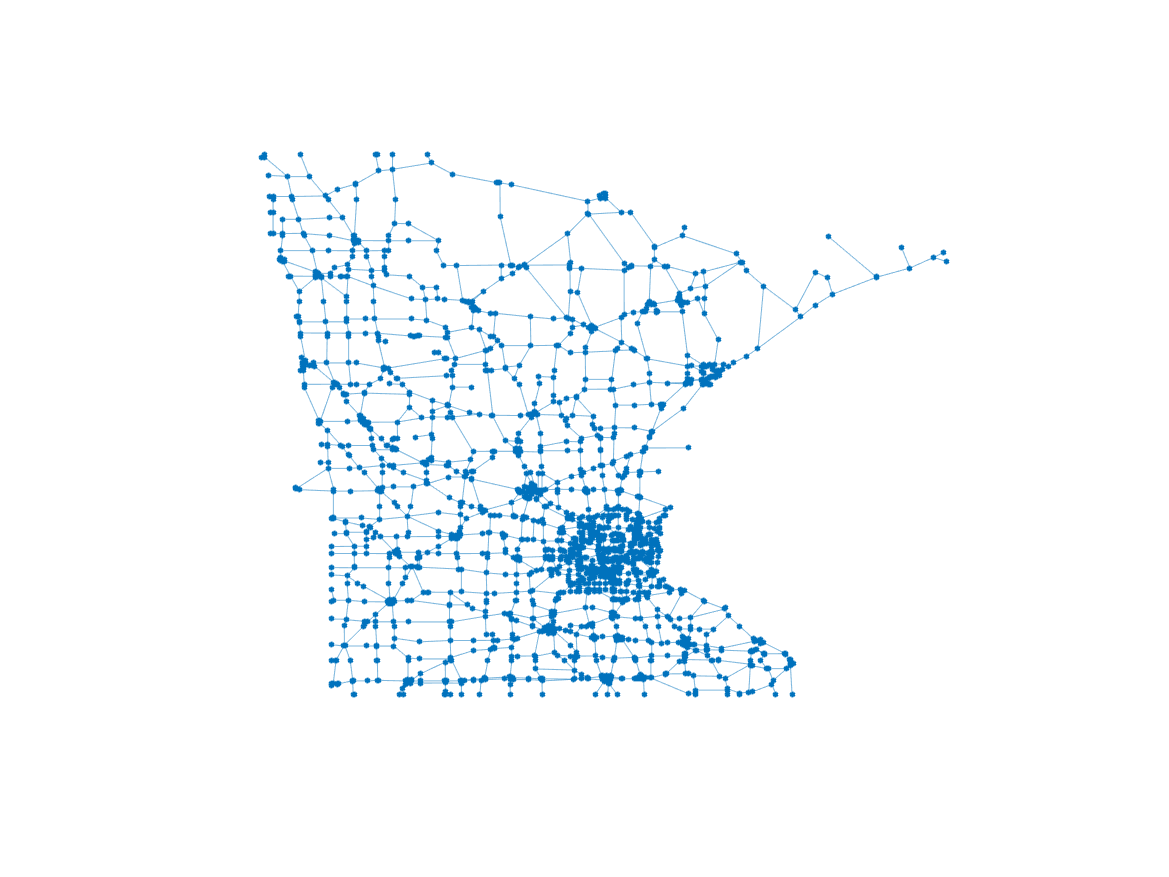
\includegraphics[scale=0.8]{Figure/minnesota}
	\caption{Grafico della rete stradale del Minnesota}
	\label{fig::minnesota}
\end{figure}
\begin{figure}[ht]
\centering
\subfloat[][$\gamma=0.10$]
{\resizebox{0.45\textwidth}{!}{% This file was created by matlab2tikz.
%
%The latest updates can be retrieved from
%  http://www.mathworks.com/matlabcentral/fileexchange/22022-matlab2tikz-matlab2tikz
%where you can also make suggestions and rate matlab2tikz.
%
\definecolor{mycolor1}{rgb}{0.00000,0.44700,0.74100}%
\definecolor{mycolor2}{rgb}{0.85000,0.32500,0.09800}%
%
\begin{tikzpicture}

\begin{axis}[%
width=0.39\columnwidth,
height=1.7in,
at={(1.011in,0.642in)},
scale only axis,
xmin=0,
xmax=1,
xlabel style={font=\color{white!15!black}},
xlabel={$\tau$},
ymin=0,
ymax=16000,
axis background/.style={fill=white},
legend columns=2,
legend pos=north west,
legend style={legend cell align=left, align=left, draw=none,fill=none}
]
\addplot [color=mycolor1, line width=2.0pt]
  table[row sep=crcr]{%
0	693\\
0.00252525252525253	693\\
0.00505050505050505	693\\
0.00757575757575758	693\\
0.0101010101010101	693\\
0.0126262626262626	693\\
0.0151515151515152	693\\
0.0176767676767677	693\\
0.0202020202020202	697\\
0.0227272727272727	701\\
0.0252525252525253	709\\
0.0277777777777778	717\\
0.0303030303030303	725\\
0.0328282828282828	733\\
0.0353535353535354	741\\
0.0378787878787879	749\\
0.0404040404040404	757\\
0.0429292929292929	765\\
0.0454545454545455	773\\
0.047979797979798	781\\
0.0505050505050505	785\\
0.053030303030303	793\\
0.0555555555555556	801\\
0.0580808080808081	809\\
0.0606060606060606	813\\
0.0631313131313131	821\\
0.0656565656565657	829\\
0.0681818181818182	833\\
0.0707070707070707	841\\
0.0732323232323232	845\\
0.0757575757575758	853\\
0.0782828282828283	861\\
0.0808080808080808	869\\
0.0833333333333333	881\\
0.0858585858585859	897\\
0.0883838383838384	913\\
0.0909090909090909	933\\
0.0934343434343434	957\\
0.095959595959596	981\\
0.0984848484848485	1001\\
0.101010101010101	1025\\
0.103535353535354	1049\\
0.106060606060606	1077\\
0.108585858585859	1101\\
0.111111111111111	1125\\
0.113636363636364	1153\\
0.116161616161616	1177\\
0.118686868686869	1205\\
0.121212121212121	1233\\
0.123737373737374	1261\\
0.126262626262626	1289\\
0.128787878787879	1317\\
0.131313131313131	1349\\
0.133838383838384	1377\\
0.136363636363636	1409\\
0.138888888888889	1441\\
0.141414141414141	1473\\
0.143939393939394	1505\\
0.146464646464646	1537\\
0.148989898989899	1569\\
0.151515151515152	1605\\
0.154040404040404	1637\\
0.156565656565657	1669\\
0.159090909090909	1701\\
0.161616161616162	1733\\
0.164141414141414	1765\\
0.166666666666667	1797\\
0.169191919191919	1829\\
0.171717171717172	1861\\
0.174242424242424	1897\\
0.176767676767677	1929\\
0.179292929292929	1961\\
0.181818181818182	1993\\
0.184343434343434	2029\\
0.186868686868687	2065\\
0.189393939393939	2097\\
0.191919191919192	2133\\
0.194444444444444	2165\\
0.196969696969697	2201\\
0.19949494949495	2237\\
0.202020202020202	2273\\
0.204545454545455	2309\\
0.207070707070707	2345\\
0.20959595959596	2381\\
0.212121212121212	2417\\
0.214646464646465	2453\\
0.217171717171717	2493\\
0.21969696969697	2533\\
0.222222222222222	2569\\
0.224747474747475	2609\\
0.227272727272727	2645\\
0.22979797979798	2685\\
0.232323232323232	2721\\
0.234848484848485	2757\\
0.237373737373737	2793\\
0.23989898989899	2829\\
0.242424242424242	2869\\
0.244949494949495	2905\\
0.247474747474747	2945\\
0.25	2981\\
0.25	2981\\
0.252525252525253	3017\\
0.255050505050505	3053\\
0.257575757575758	3093\\
0.26010101010101	3133\\
0.262626262626263	3173\\
0.265151515151515	3213\\
0.267676767676768	3253\\
0.27020202020202	3293\\
0.272727272727273	3333\\
0.275252525252525	3373\\
0.277777777777778	3413\\
0.28030303030303	3449\\
0.282828282828283	3489\\
0.285353535353535	3529\\
0.287878787878788	3569\\
0.29040404040404	3609\\
0.292929292929293	3649\\
0.295454545454545	3689\\
0.297979797979798	3729\\
0.30050505050505	3769\\
0.303030303030303	3809\\
0.305555555555556	3849\\
0.308080808080808	3889\\
0.310606060606061	3929\\
0.313131313131313	3969\\
0.315656565656566	4009\\
0.318181818181818	4045\\
0.320707070707071	4085\\
0.323232323232323	4125\\
0.325757575757576	4165\\
0.328282828282828	4205\\
0.330808080808081	4245\\
0.333333333333333	4281\\
0.335858585858586	4321\\
0.338383838383838	4361\\
0.340909090909091	4397\\
0.343434343434343	4437\\
0.345959595959596	4481\\
0.348484848484849	4525\\
0.351010101010101	4565\\
0.353535353535354	4609\\
0.356060606060606	4649\\
0.358585858585859	4689\\
0.361111111111111	4729\\
0.363636363636364	4769\\
0.366161616161616	4809\\
0.368686868686869	4849\\
0.371212121212121	4889\\
0.373737373737374	4929\\
0.376262626262626	4973\\
0.378787878787879	5013\\
0.381313131313131	5053\\
0.383838383838384	5093\\
0.386363636363636	5137\\
0.388888888888889	5177\\
0.391414141414141	5217\\
0.393939393939394	5257\\
0.396464646464646	5297\\
0.398989898989899	5341\\
0.401515151515151	5381\\
0.404040404040404	5421\\
0.406565656565657	5461\\
0.409090909090909	5501\\
0.411616161616162	5541\\
0.414141414141414	5581\\
0.416666666666667	5621\\
0.419191919191919	5661\\
0.421717171717172	5705\\
0.424242424242424	5745\\
0.426767676767677	5785\\
0.429292929292929	5825\\
0.431818181818182	5869\\
0.434343434343434	5909\\
0.436868686868687	5949\\
0.439393939393939	5993\\
0.441919191919192	6037\\
0.444444444444444	6077\\
0.446969696969697	6121\\
0.44949494949495	6161\\
0.452020202020202	6205\\
0.454545454545455	6249\\
0.457070707070707	6289\\
0.45959595959596	6333\\
0.462121212121212	6373\\
0.464646464646465	6413\\
0.467171717171717	6453\\
0.46969696969697	6497\\
0.472222222222222	6537\\
0.474747474747475	6581\\
0.477272727272727	6625\\
0.47979797979798	6669\\
0.482323232323232	6713\\
0.484848484848485	6753\\
0.487373737373737	6797\\
0.48989898989899	6841\\
0.492424242424242	6885\\
0.494949494949495	6929\\
0.497474747474748	6977\\
0.5	7021\\
0.5	7021\\
0.502525252525252	7061\\
0.505050505050505	7105\\
0.507575757575758	7149\\
0.51010101010101	7189\\
0.512626262626263	7233\\
0.515151515151515	7273\\
0.517676767676768	7317\\
0.52020202020202	7361\\
0.522727272727273	7401\\
0.525252525252525	7445\\
0.527777777777778	7485\\
0.53030303030303	7529\\
0.532828282828283	7569\\
0.535353535353535	7613\\
0.537878787878788	7653\\
0.54040404040404	7697\\
0.542929292929293	7741\\
0.545454545454545	7781\\
0.547979797979798	7825\\
0.55050505050505	7865\\
0.553030303030303	7909\\
0.555555555555556	7953\\
0.558080808080808	7997\\
0.560606060606061	8041\\
0.563131313131313	8085\\
0.565656565656566	8129\\
0.568181818181818	8169\\
0.570707070707071	8213\\
0.573232323232323	8253\\
0.575757575757576	8293\\
0.578282828282828	8337\\
0.580808080808081	8377\\
0.583333333333333	8417\\
0.585858585858586	8457\\
0.588383838383838	8501\\
0.590909090909091	8541\\
0.593434343434343	8585\\
0.595959595959596	8629\\
0.598484848484849	8669\\
0.601010101010101	8713\\
0.603535353535354	8757\\
0.606060606060606	8801\\
0.608585858585859	8845\\
0.611111111111111	8885\\
0.613636363636364	8929\\
0.616161616161616	8977\\
0.618686868686869	9021\\
0.621212121212121	9065\\
0.623737373737374	9109\\
0.626262626262626	9153\\
0.628787878787879	9197\\
0.631313131313131	9241\\
0.633838383838384	9285\\
0.636363636363636	9329\\
0.638888888888889	9369\\
0.641414141414141	9413\\
0.643939393939394	9457\\
0.646464646464646	9501\\
0.648989898989899	9545\\
0.651515151515151	9589\\
0.654040404040404	9633\\
0.656565656565657	9677\\
0.659090909090909	9721\\
0.661616161616162	9765\\
0.664141414141414	9809\\
0.666666666666667	9853\\
0.669191919191919	9897\\
0.671717171717172	9945\\
0.674242424242424	9989\\
0.676767676767677	10037\\
0.679292929292929	10081\\
0.681818181818182	10125\\
0.684343434343434	10169\\
0.686868686868687	10213\\
0.689393939393939	10257\\
0.691919191919192	10297\\
0.694444444444444	10341\\
0.696969696969697	10381\\
0.69949494949495	10425\\
0.702020202020202	10469\\
0.704545454545455	10509\\
0.707070707070707	10553\\
0.70959595959596	10597\\
0.712121212121212	10641\\
0.714646464646465	10681\\
0.717171717171717	10725\\
0.71969696969697	10773\\
0.722222222222222	10817\\
0.724747474747475	10861\\
0.727272727272727	10905\\
0.72979797979798	10953\\
0.732323232323232	10997\\
0.734848484848485	11041\\
0.737373737373737	11085\\
0.73989898989899	11133\\
0.742424242424242	11177\\
0.744949494949495	11221\\
0.747474747474748	11265\\
0.75	11309\\
0.75	11309\\
0.752525252525252	11353\\
0.755050505050505	11397\\
0.757575757575758	11441\\
0.76010101010101	11481\\
0.762626262626263	11525\\
0.765151515151515	11565\\
0.767676767676768	11613\\
0.77020202020202	11657\\
0.772727272727273	11705\\
0.775252525252525	11749\\
0.777777777777778	11797\\
0.78030303030303	11841\\
0.782828282828283	11889\\
0.785353535353535	11933\\
0.787878787878788	11977\\
0.79040404040404	12021\\
0.792929292929293	12065\\
0.795454545454545	12109\\
0.797979797979798	12153\\
0.80050505050505	12193\\
0.803030303030303	12233\\
0.805555555555556	12277\\
0.808080808080808	12317\\
0.810606060606061	12357\\
0.813131313131313	12401\\
0.815656565656566	12441\\
0.818181818181818	12485\\
0.820707070707071	12529\\
0.823232323232323	12577\\
0.825757575757576	12621\\
0.828282828282828	12669\\
0.830808080808081	12713\\
0.833333333333333	12761\\
0.835858585858586	12805\\
0.838383838383838	12853\\
0.840909090909091	12897\\
0.843434343434343	12941\\
0.845959595959596	12985\\
0.848484848484849	13029\\
0.851010101010101	13073\\
0.853535353535354	13117\\
0.856060606060606	13161\\
0.858585858585859	13201\\
0.861111111111111	13241\\
0.863636363636364	13281\\
0.866161616161616	13321\\
0.868686868686869	13361\\
0.871212121212121	13397\\
0.873737373737374	13437\\
0.876262626262626	13477\\
0.878787878787879	13517\\
0.881313131313131	13557\\
0.883838383838384	13601\\
0.886363636363636	13645\\
0.888888888888889	13693\\
0.891414141414141	13737\\
0.893939393939394	13781\\
0.896464646464646	13825\\
0.898989898989899	13873\\
0.901515151515151	13917\\
0.904040404040404	13957\\
0.906565656565657	14001\\
0.909090909090909	14041\\
0.911616161616162	14081\\
0.914141414141414	14121\\
0.916666666666667	14161\\
0.919191919191919	14197\\
0.921717171717172	14237\\
0.924242424242424	14277\\
0.926767676767677	14317\\
0.929292929292929	14357\\
0.931818181818182	14401\\
0.934343434343434	14445\\
0.936868686868687	14489\\
0.939393939393939	14533\\
0.941919191919192	14577\\
0.944444444444444	14617\\
0.946969696969697	14661\\
0.94949494949495	14701\\
0.952020202020202	14741\\
0.954545454545455	14781\\
0.957070707070707	14821\\
0.95959595959596	14861\\
0.962121212121212	14897\\
0.964646464646465	14937\\
0.967171717171717	14973\\
0.96969696969697	15013\\
0.972222222222222	15049\\
0.974747474747475	15085\\
0.977272727272727	15125\\
0.97979797979798	15165\\
0.982323232323232	15205\\
0.984848484848485	15245\\
0.987373737373737	15285\\
0.98989898989899	15325\\
0.992424242424242	15365\\
0.994949494949495	15405\\
0.997474747474748	15445\\
1	15485\\
};
\addlegendentry{ode45}

\addplot [color=mycolor2, line width=2.0pt]
  table[row sep=crcr]{%
0	253\\
0.00252525252525253	253\\
0.00505050505050505	253\\
0.00757575757575758	253\\
0.0101010101010101	253\\
0.0126262626262626	255\\
0.0151515151515152	259\\
0.0176767676767677	265\\
0.0202020202020202	271\\
0.0227272727272727	277\\
0.0252525252525253	282\\
0.0277777777777778	288\\
0.0303030303030303	295\\
0.0328282828282828	300\\
0.0353535353535354	305\\
0.0378787878787879	311\\
0.0404040404040404	312\\
0.0429292929292929	320\\
0.0454545454545455	324\\
0.047979797979798	329\\
0.0505050505050505	333\\
0.053030303030303	338\\
0.0555555555555556	342\\
0.0580808080808081	346\\
0.0606060606060606	350\\
0.0631313131313131	354\\
0.0656565656565657	358\\
0.0681818181818182	361\\
0.0707070707070707	365\\
0.0732323232323232	369\\
0.0757575757575758	373\\
0.0782828282828283	380\\
0.0808080808080808	387\\
0.0833333333333333	395\\
0.0858585858585859	403\\
0.0883838383838384	415\\
0.0909090909090909	424\\
0.0934343434343434	434\\
0.095959595959596	443\\
0.0984848484848485	454\\
0.101010101010101	464\\
0.103535353535354	475\\
0.106060606060606	486\\
0.108585858585859	497\\
0.111111111111111	509\\
0.113636363636364	522\\
0.116161616161616	529\\
0.118686868686869	543\\
0.121212121212121	557\\
0.123737373737374	574\\
0.126262626262626	588\\
0.128787878787879	597\\
0.131313131313131	611\\
0.133838383838384	625\\
0.136363636363636	638\\
0.138888888888889	652\\
0.141414141414141	665\\
0.143939393939394	679\\
0.146464646464646	692\\
0.148989898989899	706\\
0.151515151515152	719\\
0.154040404040404	732\\
0.156565656565657	745\\
0.159090909090909	759\\
0.161616161616162	773\\
0.164141414141414	786\\
0.166666666666667	800\\
0.169191919191919	813\\
0.171717171717172	826\\
0.174242424242424	840\\
0.176767676767677	853\\
0.179292929292929	866\\
0.181818181818182	880\\
0.184343434343434	894\\
0.186868686868687	908\\
0.189393939393939	922\\
0.191919191919192	935\\
0.194444444444444	949\\
0.196969696969697	962\\
0.19949494949495	976\\
0.202020202020202	989\\
0.204545454545455	1002\\
0.207070707070707	1017\\
0.20959595959596	1031\\
0.212121212121212	1044\\
0.214646464646465	1059\\
0.217171717171717	1072\\
0.21969696969697	1088\\
0.222222222222222	1099\\
0.224747474747475	1115\\
0.227272727272727	1128\\
0.22979797979798	1145\\
0.232323232323232	1157\\
0.234848484848485	1169\\
0.237373737373737	1186\\
0.23989898989899	1204\\
0.242424242424242	1219\\
0.244949494949495	1236\\
0.247474747474747	1252\\
0.25	1272\\
0.25	1272\\
0.252525252525253	1289\\
0.255050505050505	1302\\
0.257575757575758	1319\\
0.26010101010101	1335\\
0.262626262626263	1351\\
0.265151515151515	1366\\
0.267676767676768	1380\\
0.27020202020202	1395\\
0.272727272727273	1409\\
0.275252525252525	1424\\
0.277777777777778	1439\\
0.28030303030303	1453\\
0.282828282828283	1467\\
0.285353535353535	1481\\
0.287878787878788	1496\\
0.29040404040404	1511\\
0.292929292929293	1526\\
0.295454545454545	1541\\
0.297979797979798	1555\\
0.30050505050505	1570\\
0.303030303030303	1585\\
0.305555555555556	1600\\
0.308080808080808	1614\\
0.310606060606061	1629\\
0.313131313131313	1644\\
0.315656565656566	1660\\
0.318181818181818	1675\\
0.320707070707071	1693\\
0.323232323232323	1711\\
0.325757575757576	1729\\
0.328282828282828	1745\\
0.330808080808081	1762\\
0.333333333333333	1779\\
0.335858585858586	1794\\
0.338383838383838	1810\\
0.340909090909091	1825\\
0.343434343434343	1844\\
0.345959595959596	1860\\
0.348484848484849	1876\\
0.351010101010101	1890\\
0.353535353535354	1907\\
0.356060606060606	1922\\
0.358585858585859	1938\\
0.361111111111111	1953\\
0.363636363636364	1970\\
0.366161616161616	1988\\
0.368686868686869	2005\\
0.371212121212121	2021\\
0.373737373737374	2033\\
0.376262626262626	2051\\
0.378787878787879	2067\\
0.381313131313131	2083\\
0.383838383838384	2099\\
0.386363636363636	2114\\
0.388888888888889	2130\\
0.391414141414141	2144\\
0.393939393939394	2160\\
0.396464646464646	2176\\
0.398989898989899	2194\\
0.401515151515151	2207\\
0.404040404040404	2222\\
0.406565656565657	2239\\
0.409090909090909	2255\\
0.411616161616162	2271\\
0.414141414141414	2287\\
0.416666666666667	2304\\
0.419191919191919	2317\\
0.421717171717172	2332\\
0.424242424242424	2349\\
0.426767676767677	2365\\
0.429292929292929	2381\\
0.431818181818182	2398\\
0.434343434343434	2410\\
0.436868686868687	2424\\
0.439393939393939	2438\\
0.441919191919192	2453\\
0.444444444444444	2471\\
0.446969696969697	2493\\
0.44949494949495	2519\\
0.452020202020202	2532\\
0.454545454545455	2542\\
0.457070707070707	2559\\
0.45959595959596	2577\\
0.462121212121212	2596\\
0.464646464646465	2613\\
0.467171717171717	2628\\
0.46969696969697	2655\\
0.472222222222222	2670\\
0.474747474747475	2682\\
0.477272727272727	2698\\
0.47979797979798	2715\\
0.482323232323232	2732\\
0.484848484848485	2745\\
0.487373737373737	2757\\
0.48989898989899	2776\\
0.492424242424242	2792\\
0.494949494949495	2827\\
0.497474747474748	2844\\
0.5	2848\\
0.5	2848\\
0.502525252525252	2865\\
0.505050505050505	2881\\
0.507575757575758	2896\\
0.51010101010101	2917\\
0.512626262626263	2933\\
0.515151515151515	2946\\
0.517676767676768	2964\\
0.52020202020202	2979\\
0.522727272727273	2997\\
0.525252525252525	3014\\
0.527777777777778	3028\\
0.53030303030303	3048\\
0.532828282828283	3063\\
0.535353535353535	3081\\
0.537878787878788	3097\\
0.54040404040404	3114\\
0.542929292929293	3126\\
0.545454545454545	3143\\
0.547979797979798	3159\\
0.55050505050505	3175\\
0.553030303030303	3193\\
0.555555555555556	3211\\
0.558080808080808	3227\\
0.560606060606061	3244\\
0.563131313131313	3262\\
0.565656565656566	3269\\
0.568181818181818	3283\\
0.570707070707071	3301\\
0.573232323232323	3328\\
0.575757575757576	3340\\
0.578282828282828	3357\\
0.580808080808081	3374\\
0.583333333333333	3391\\
0.585858585858586	3418\\
0.588383838383838	3430\\
0.590909090909091	3443\\
0.593434343434343	3460\\
0.595959595959596	3474\\
0.598484848484849	3495\\
0.601010101010101	3512\\
0.603535353535354	3529\\
0.606060606060606	3540\\
0.608585858585859	3561\\
0.611111111111111	3573\\
0.613636363636364	3595\\
0.616161616161616	3611\\
0.618686868686869	3627\\
0.621212121212121	3643\\
0.623737373737374	3659\\
0.626262626262626	3680\\
0.628787878787879	3703\\
0.631313131313131	3719\\
0.633838383838384	3741\\
0.636363636363636	3755\\
0.638888888888889	3771\\
0.641414141414141	3790\\
0.643939393939394	3812\\
0.646464646464646	3825\\
0.648989898989899	3843\\
0.651515151515151	3864\\
0.654040404040404	3883\\
0.656565656565657	3901\\
0.659090909090909	3918\\
0.661616161616162	3932\\
0.664141414141414	3951\\
0.666666666666667	3967\\
0.669191919191919	3985\\
0.671717171717172	4004\\
0.674242424242424	4024\\
0.676767676767677	4043\\
0.679292929292929	4062\\
0.681818181818182	4081\\
0.684343434343434	4099\\
0.686868686868687	4112\\
0.689393939393939	4132\\
0.691919191919192	4144\\
0.694444444444444	4151\\
0.696969696969697	4168\\
0.69949494949495	4198\\
0.702020202020202	4210\\
0.704545454545455	4225\\
0.707070707070707	4239\\
0.70959595959596	4254\\
0.712121212121212	4271\\
0.714646464646465	4286\\
0.717171717171717	4303\\
0.71969696969697	4317\\
0.722222222222222	4337\\
0.724747474747475	4357\\
0.727272727272727	4374\\
0.72979797979798	4392\\
0.732323232323232	4412\\
0.734848484848485	4431\\
0.737373737373737	4447\\
0.73989898989899	4467\\
0.742424242424242	4487\\
0.744949494949495	4506\\
0.747474747474748	4523\\
0.75	4542\\
0.75	4542\\
0.752525252525252	4560\\
0.755050505050505	4576\\
0.757575757575758	4599\\
0.76010101010101	4625\\
0.762626262626263	4646\\
0.765151515151515	4675\\
0.767676767676768	4711\\
0.77020202020202	4754\\
0.772727272727273	4809\\
0.775252525252525	4875\\
0.777777777777778	4968\\
0.78030303030303	5101\\
0.782828282828283	5423\\
0.785353535353535	10728\\
0.787878787878788	10726\\
0.79040404040404	10725\\
0.792929292929293	10722\\
0.795454545454545	10719\\
0.797979797979798	10718\\
0.80050505050505	10716\\
0.803030303030303	10711\\
0.805555555555556	10712\\
0.808080808080808	10710\\
0.810606060606061	10708\\
0.813131313131313	10706\\
0.815656565656566	10706\\
0.818181818181818	10704\\
0.820707070707071	10703\\
0.823232323232323	10700\\
0.825757575757576	10700\\
0.828282828282828	10698\\
0.830808080808081	10697\\
0.833333333333333	10695\\
0.835858585858586	10696\\
0.838383838383838	10694\\
0.840909090909091	10693\\
0.843434343434343	10691\\
0.845959595959596	10693\\
0.848484848484849	10687\\
0.851010101010101	10690\\
0.853535353535354	10685\\
0.856060606060606	10686\\
0.858585858585859	10685\\
0.861111111111111	10685\\
0.863636363636364	10681\\
0.866161616161616	10684\\
0.868686868686869	10678\\
0.871212121212121	5339\\
0.873737373737374	5357\\
0.876262626262626	5376\\
0.878787878787879	5391\\
0.881313131313131	5401\\
0.883838383838384	5423\\
0.886363636363636	10925\\
0.888888888888889	10964\\
0.891414141414141	10950\\
0.893939393939394	10966\\
0.896464646464646	10953\\
0.898989898989899	10972\\
0.901515151515151	10956\\
0.904040404040404	11030\\
0.906565656565657	10961\\
0.909090909090909	11042\\
0.911616161616162	11019\\
0.914141414141414	10951\\
0.916666666666667	11032\\
0.919191919191919	11010\\
0.921717171717172	10950\\
0.924242424242424	11021\\
0.926767676767677	10998\\
0.929292929292929	10980\\
0.931818181818182	10931\\
0.934343434343434	10974\\
0.936868686868687	10977\\
0.939393939393939	10928\\
0.941919191919192	10915\\
0.944444444444444	10952\\
0.946969696969697	10940\\
0.94949494949495	10898\\
0.952020202020202	10940\\
0.954545454545455	10931\\
0.957070707070707	10920\\
0.95959595959596	10884\\
0.962121212121212	10879\\
0.964646464646465	10906\\
0.967171717171717	10894\\
0.96969696969697	10886\\
0.972222222222222	10870\\
0.974747474747475	10866\\
0.977272727272727	10884\\
0.97979797979798	10879\\
0.982323232323232	10875\\
0.984848484848485	10849\\
0.987373737373737	10845\\
0.98989898989899	10875\\
0.992424242424242	10872\\
0.994949494949495	10866\\
0.997474747474748	10842\\
1	10845\\
};
\addlegendentry{ode15s}
\end{axis}
\end{tikzpicture}%}}
 \quad 
\subfloat[][$\gamma=0.30$]
{\resizebox{0.45\textwidth}{!}{ % This file was created by matlab2tikz.
%
%The latest updates can be retrieved from
%  http://www.mathworks.com/matlabcentral/fileexchange/22022-matlab2tikz-matlab2tikz
%where you can also make suggestions and rate matlab2tikz.
%
\definecolor{mycolor1}{rgb}{0.00000,0.44700,0.74100}%
\definecolor{mycolor2}{rgb}{0.85000,0.32500,0.09800}%
%
\begin{tikzpicture}

\begin{axis}[%
width=0.39\columnwidth,
height=1.7in,
at={(1.011in,0.642in)},
scale only axis,
xmin=0,
xmax=1,
xlabel style={font=\color{white!15!black}},
xlabel={$\tau$},
ymin=0,
ymax=14000,
legend columns=2,
legend pos=north west,
legend style={legend cell align=left, align=left, draw=none,fill=none}
]
\addplot [color=mycolor1, line width=2.0pt]
  table[row sep=crcr]{%
0	1281\\
0.00252525252525253	1281\\
0.00505050505050505	1281\\
0.00757575757575758	1281\\
0.0101010101010101	1281\\
0.0126262626262626	1281\\
0.0151515151515152	1281\\
0.0176767676767677	1281\\
0.0202020202020202	1281\\
0.0227272727272727	1281\\
0.0252525252525253	1281\\
0.0277777777777778	1281\\
0.0303030303030303	1281\\
0.0328282828282828	1281\\
0.0353535353535354	1281\\
0.0378787878787879	1281\\
0.0404040404040404	1281\\
0.0429292929292929	1281\\
0.0454545454545455	1281\\
0.047979797979798	1281\\
0.0505050505050505	1281\\
0.053030303030303	1281\\
0.0555555555555556	1281\\
0.0580808080808081	1285\\
0.0606060606060606	1285\\
0.0631313131313131	1289\\
0.0656565656565657	1289\\
0.0681818181818182	1293\\
0.0707070707070707	1293\\
0.0732323232323232	1297\\
0.0757575757575758	1297\\
0.0782828282828283	1301\\
0.0808080808080808	1305\\
0.0833333333333333	1305\\
0.0858585858585859	1309\\
0.0883838383838384	1309\\
0.0909090909090909	1313\\
0.0934343434343434	1317\\
0.095959595959596	1317\\
0.0984848484848485	1321\\
0.101010101010101	1325\\
0.103535353535354	1325\\
0.106060606060606	1329\\
0.108585858585859	1333\\
0.111111111111111	1333\\
0.113636363636364	1337\\
0.116161616161616	1341\\
0.118686868686869	1341\\
0.121212121212121	1345\\
0.123737373737374	1349\\
0.126262626262626	1349\\
0.128787878787879	1353\\
0.131313131313131	1357\\
0.133838383838384	1357\\
0.136363636363636	1361\\
0.138888888888889	1365\\
0.141414141414141	1365\\
0.143939393939394	1369\\
0.146464646464646	1373\\
0.148989898989899	1381\\
0.151515151515152	1389\\
0.154040404040404	1397\\
0.156565656565657	1405\\
0.159090909090909	1413\\
0.161616161616162	1425\\
0.164141414141414	1433\\
0.166666666666667	1445\\
0.169191919191919	1457\\
0.171717171717172	1473\\
0.174242424242424	1485\\
0.176767676767677	1497\\
0.179292929292929	1513\\
0.181818181818182	1529\\
0.184343434343434	1541\\
0.186868686868687	1557\\
0.189393939393939	1573\\
0.191919191919192	1589\\
0.194444444444444	1605\\
0.196969696969697	1621\\
0.19949494949495	1637\\
0.202020202020202	1653\\
0.204545454545455	1673\\
0.207070707070707	1689\\
0.20959595959596	1709\\
0.212121212121212	1729\\
0.214646464646465	1749\\
0.217171717171717	1773\\
0.21969696969697	1793\\
0.222222222222222	1817\\
0.224747474747475	1837\\
0.227272727272727	1861\\
0.22979797979798	1885\\
0.232323232323232	1909\\
0.234848484848485	1933\\
0.237373737373737	1957\\
0.23989898989899	1981\\
0.242424242424242	2005\\
0.244949494949495	2029\\
0.247474747474747	2057\\
0.25	2081\\
0.25	2081\\
0.252525252525253	2109\\
0.255050505050505	2137\\
0.257575757575758	2169\\
0.26010101010101	2197\\
0.262626262626263	2229\\
0.265151515151515	2261\\
0.267676767676768	2293\\
0.27020202020202	2321\\
0.272727272727273	2353\\
0.275252525252525	2381\\
0.277777777777778	2413\\
0.28030303030303	2441\\
0.282828282828283	2469\\
0.285353535353535	2501\\
0.287878787878788	2529\\
0.29040404040404	2561\\
0.292929292929293	2589\\
0.295454545454545	2621\\
0.297979797979798	2653\\
0.30050505050505	2681\\
0.303030303030303	2713\\
0.305555555555556	2741\\
0.308080808080808	2773\\
0.310606060606061	2805\\
0.313131313131313	2837\\
0.315656565656566	2865\\
0.318181818181818	2897\\
0.320707070707071	2929\\
0.323232323232323	2961\\
0.325757575757576	2993\\
0.328282828282828	3021\\
0.330808080808081	3053\\
0.333333333333333	3085\\
0.335858585858586	3117\\
0.338383838383838	3153\\
0.340909090909091	3185\\
0.343434343434343	3221\\
0.345959595959596	3257\\
0.348484848484849	3293\\
0.351010101010101	3329\\
0.353535353535354	3365\\
0.356060606060606	3401\\
0.358585858585859	3433\\
0.361111111111111	3465\\
0.363636363636364	3501\\
0.366161616161616	3533\\
0.368686868686869	3569\\
0.371212121212121	3601\\
0.373737373737374	3637\\
0.376262626262626	3673\\
0.378787878787879	3705\\
0.381313131313131	3741\\
0.383838383838384	3773\\
0.386363636363636	3809\\
0.388888888888889	3841\\
0.391414141414141	3873\\
0.393939393939394	3909\\
0.396464646464646	3941\\
0.398989898989899	3977\\
0.401515151515151	4009\\
0.404040404040404	4045\\
0.406565656565657	4077\\
0.409090909090909	4113\\
0.411616161616162	4145\\
0.414141414141414	4181\\
0.416666666666667	4213\\
0.419191919191919	4249\\
0.421717171717172	4285\\
0.424242424242424	4317\\
0.426767676767677	4353\\
0.429292929292929	4389\\
0.431818181818182	4425\\
0.434343434343434	4461\\
0.436868686868687	4497\\
0.439393939393939	4533\\
0.441919191919192	4569\\
0.444444444444444	4605\\
0.446969696969697	4641\\
0.44949494949495	4677\\
0.452020202020202	4709\\
0.454545454545455	4745\\
0.457070707070707	4781\\
0.45959595959596	4813\\
0.462121212121212	4849\\
0.464646464646465	4889\\
0.467171717171717	4925\\
0.46969696969697	4965\\
0.472222222222222	5001\\
0.474747474747475	5041\\
0.477272727272727	5081\\
0.47979797979798	5121\\
0.482323232323232	5157\\
0.484848484848485	5197\\
0.487373737373737	5237\\
0.48989898989899	5277\\
0.492424242424242	5317\\
0.494949494949495	5361\\
0.497474747474748	5401\\
0.5	5441\\
0.5	5441\\
0.502525252525252	5481\\
0.505050505050505	5521\\
0.507575757575758	5557\\
0.51010101010101	5593\\
0.512626262626263	5633\\
0.515151515151515	5669\\
0.517676767676768	5709\\
0.52020202020202	5745\\
0.522727272727273	5785\\
0.525252525252525	5821\\
0.527777777777778	5861\\
0.53030303030303	5897\\
0.532828282828283	5937\\
0.535353535353535	5973\\
0.537878787878788	6013\\
0.54040404040404	6053\\
0.542929292929293	6093\\
0.545454545454545	6129\\
0.547979797979798	6169\\
0.55050505050505	6209\\
0.553030303030303	6249\\
0.555555555555556	6289\\
0.558080808080808	6329\\
0.560606060606061	6369\\
0.563131313131313	6409\\
0.565656565656566	6445\\
0.568181818181818	6485\\
0.570707070707071	6521\\
0.573232323232323	6557\\
0.575757575757576	6597\\
0.578282828282828	6633\\
0.580808080808081	6669\\
0.583333333333333	6705\\
0.585858585858586	6745\\
0.588383838383838	6781\\
0.590909090909091	6821\\
0.593434343434343	6857\\
0.595959595959596	6893\\
0.598484848484849	6933\\
0.601010101010101	6973\\
0.603535353535354	7013\\
0.606060606060606	7049\\
0.608585858585859	7089\\
0.611111111111111	7129\\
0.613636363636364	7169\\
0.616161616161616	7209\\
0.618686868686869	7249\\
0.621212121212121	7289\\
0.623737373737374	7329\\
0.626262626262626	7373\\
0.628787878787879	7413\\
0.631313131313131	7453\\
0.633838383838384	7493\\
0.636363636363636	7533\\
0.638888888888889	7573\\
0.641414141414141	7613\\
0.643939393939394	7649\\
0.646464646464646	7689\\
0.648989898989899	7729\\
0.651515151515151	7769\\
0.654040404040404	7813\\
0.656565656565657	7853\\
0.659090909090909	7893\\
0.661616161616162	7933\\
0.664141414141414	7973\\
0.666666666666667	8017\\
0.669191919191919	8061\\
0.671717171717172	8105\\
0.674242424242424	8149\\
0.676767676767677	8193\\
0.679292929292929	8237\\
0.681818181818182	8277\\
0.684343434343434	8321\\
0.686868686868687	8361\\
0.689393939393939	8401\\
0.691919191919192	8441\\
0.694444444444444	8481\\
0.696969696969697	8521\\
0.69949494949495	8561\\
0.702020202020202	8605\\
0.704545454545455	8645\\
0.707070707070707	8685\\
0.70959595959596	8725\\
0.712121212121212	8769\\
0.714646464646465	8809\\
0.717171717171717	8853\\
0.71969696969697	8897\\
0.722222222222222	8941\\
0.724747474747475	8981\\
0.727272727272727	9025\\
0.72979797979798	9069\\
0.732323232323232	9113\\
0.734848484848485	9157\\
0.737373737373737	9197\\
0.73989898989899	9241\\
0.742424242424242	9285\\
0.744949494949495	9325\\
0.747474747474748	9369\\
0.75	9409\\
0.75	9409\\
0.752525252525252	9453\\
0.755050505050505	9493\\
0.757575757575758	9533\\
0.76010101010101	9573\\
0.762626262626263	9617\\
0.765151515151515	9657\\
0.767676767676768	9701\\
0.77020202020202	9745\\
0.772727272727273	9785\\
0.775252525252525	9829\\
0.777777777777778	9873\\
0.78030303030303	9913\\
0.782828282828283	9957\\
0.785353535353535	10001\\
0.787878787878788	10041\\
0.79040404040404	10085\\
0.792929292929293	10125\\
0.795454545454545	10169\\
0.797979797979798	10209\\
0.80050505050505	10249\\
0.803030303030303	10293\\
0.805555555555556	10333\\
0.808080808080808	10373\\
0.810606060606061	10413\\
0.813131313131313	10457\\
0.815656565656566	10497\\
0.818181818181818	10541\\
0.820707070707071	10589\\
0.823232323232323	10633\\
0.825757575757576	10673\\
0.828282828282828	10721\\
0.830808080808081	10765\\
0.833333333333333	10809\\
0.835858585858586	10857\\
0.838383838383838	10901\\
0.840909090909091	10945\\
0.843434343434343	10989\\
0.845959595959596	11029\\
0.848484848484849	11073\\
0.851010101010101	11113\\
0.853535353535354	11153\\
0.856060606060606	11193\\
0.858585858585859	11233\\
0.861111111111111	11273\\
0.863636363636364	11313\\
0.866161616161616	11357\\
0.868686868686869	11401\\
0.871212121212121	11441\\
0.873737373737374	11489\\
0.876262626262626	11533\\
0.878787878787879	11577\\
0.881313131313131	11621\\
0.883838383838384	11665\\
0.886363636363636	11709\\
0.888888888888889	11749\\
0.891414141414141	11793\\
0.893939393939394	11837\\
0.896464646464646	11881\\
0.898989898989899	11925\\
0.901515151515151	11969\\
0.904040404040404	12009\\
0.906565656565657	12049\\
0.909090909090909	12085\\
0.911616161616162	12125\\
0.914141414141414	12161\\
0.916666666666667	12197\\
0.919191919191919	12237\\
0.921717171717172	12273\\
0.924242424242424	12313\\
0.926767676767677	12349\\
0.929292929292929	12393\\
0.931818181818182	12433\\
0.934343434343434	12477\\
0.936868686868687	12521\\
0.939393939393939	12565\\
0.941919191919192	12609\\
0.944444444444444	12653\\
0.946969696969697	12693\\
0.94949494949495	12737\\
0.952020202020202	12777\\
0.954545454545455	12817\\
0.957070707070707	12857\\
0.95959595959596	12893\\
0.962121212121212	12933\\
0.964646464646465	12969\\
0.967171717171717	13005\\
0.96969696969697	13041\\
0.972222222222222	13081\\
0.974747474747475	13121\\
0.977272727272727	13161\\
0.97979797979798	13201\\
0.982323232323232	13245\\
0.984848484848485	13289\\
0.987373737373737	13329\\
0.98989898989899	13373\\
0.992424242424242	13413\\
0.994949494949495	13449\\
0.997474747474748	13489\\
1	13529\\
};
\addlegendentry{ode45}

\addplot [color=mycolor2, line width=2.0pt]
  table[row sep=crcr]{%
0	464\\
0.00252525252525253	464\\
0.00505050505050505	464\\
0.00757575757575758	464\\
0.0101010101010101	464\\
0.0126262626262626	464\\
0.0151515151515152	464\\
0.0176767676767677	464\\
0.0202020202020202	464\\
0.0227272727272727	464\\
0.0252525252525253	464\\
0.0277777777777778	464\\
0.0303030303030303	465\\
0.0328282828282828	465\\
0.0353535353535354	466\\
0.0378787878787879	467\\
0.0404040404040404	468\\
0.0429292929292929	469\\
0.0454545454545455	470\\
0.047979797979798	471\\
0.0505050505050505	473\\
0.053030303030303	475\\
0.0555555555555556	477\\
0.0580808080808081	479\\
0.0606060606060606	481\\
0.0631313131313131	483\\
0.0656565656565657	485\\
0.0681818181818182	487\\
0.0707070707070707	489\\
0.0732323232323232	491\\
0.0757575757575758	493\\
0.0782828282828283	495\\
0.0808080808080808	497\\
0.0833333333333333	499\\
0.0858585858585859	501\\
0.0883838383838384	503\\
0.0909090909090909	505\\
0.0934343434343434	506\\
0.095959595959596	508\\
0.0984848484848485	510\\
0.101010101010101	512\\
0.103535353535354	514\\
0.106060606060606	515\\
0.108585858585859	517\\
0.111111111111111	519\\
0.113636363636364	521\\
0.116161616161616	522\\
0.118686868686869	524\\
0.121212121212121	526\\
0.123737373737374	527\\
0.126262626262626	529\\
0.128787878787879	530\\
0.131313131313131	532\\
0.133838383838384	533\\
0.136363636363636	532\\
0.138888888888889	534\\
0.141414141414141	535\\
0.143939393939394	537\\
0.146464646464646	539\\
0.148989898989899	542\\
0.151515151515152	548\\
0.154040404040404	551\\
0.156565656565657	554\\
0.159090909090909	559\\
0.161616161616162	564\\
0.164141414141414	570\\
0.166666666666667	578\\
0.169191919191919	586\\
0.171717171717172	595\\
0.174242424242424	603\\
0.176767676767677	611\\
0.179292929292929	619\\
0.181818181818182	627\\
0.184343434343434	636\\
0.186868686868687	645\\
0.189393939393939	654\\
0.191919191919192	663\\
0.194444444444444	672\\
0.196969696969697	682\\
0.19949494949495	692\\
0.202020202020202	701\\
0.204545454545455	711\\
0.207070707070707	721\\
0.20959595959596	738\\
0.212121212121212	741\\
0.214646464646465	761\\
0.217171717171717	774\\
0.21969696969697	786\\
0.222222222222222	800\\
0.224747474747475	811\\
0.227272727272727	826\\
0.22979797979798	828\\
0.232323232323232	853\\
0.234848484848485	866\\
0.237373737373737	880\\
0.23989898989899	874\\
0.242424242424242	886\\
0.244949494949495	898\\
0.247474747474747	910\\
0.25	922\\
0.25	922\\
0.252525252525253	934\\
0.255050505050505	946\\
0.257575757575758	959\\
0.26010101010101	972\\
0.262626262626263	983\\
0.265151515151515	996\\
0.267676767676768	1009\\
0.27020202020202	1022\\
0.272727272727273	1042\\
0.275252525252525	1055\\
0.277777777777778	1070\\
0.28030303030303	1087\\
0.282828282828283	1101\\
0.285353535353535	1109\\
0.287878787878788	1124\\
0.29040404040404	1140\\
0.292929292929293	1155\\
0.295454545454545	1172\\
0.297979797979798	1189\\
0.30050505050505	1204\\
0.303030303030303	1222\\
0.305555555555556	1237\\
0.308080808080808	1254\\
0.310606060606061	1269\\
0.313131313131313	1283\\
0.315656565656566	1299\\
0.318181818181818	1312\\
0.320707070707071	1328\\
0.323232323232323	1342\\
0.325757575757576	1355\\
0.328282828282828	1369\\
0.330808080808081	1384\\
0.333333333333333	1397\\
0.335858585858586	1410\\
0.338383838383838	1425\\
0.340909090909091	1438\\
0.343434343434343	1452\\
0.345959595959596	1466\\
0.348484848484849	1479\\
0.351010101010101	1493\\
0.353535353535354	1509\\
0.356060606060606	1522\\
0.358585858585859	1535\\
0.361111111111111	1549\\
0.363636363636364	1564\\
0.366161616161616	1579\\
0.368686868686869	1595\\
0.371212121212121	1611\\
0.373737373737374	1630\\
0.376262626262626	1645\\
0.378787878787879	1662\\
0.381313131313131	1677\\
0.383838383838384	1693\\
0.386363636363636	1709\\
0.388888888888889	1724\\
0.391414141414141	1740\\
0.393939393939394	1756\\
0.396464646464646	1773\\
0.398989898989899	1787\\
0.401515151515151	1801\\
0.404040404040404	1816\\
0.406565656565657	1832\\
0.409090909090909	1849\\
0.411616161616162	1863\\
0.414141414141414	1879\\
0.416666666666667	1895\\
0.419191919191919	1911\\
0.421717171717172	1926\\
0.424242424242424	1942\\
0.426767676767677	1957\\
0.429292929292929	1973\\
0.431818181818182	1993\\
0.434343434343434	2007\\
0.436868686868687	2023\\
0.439393939393939	2039\\
0.441919191919192	2055\\
0.444444444444444	2066\\
0.446969696969697	2082\\
0.44949494949495	2096\\
0.452020202020202	2111\\
0.454545454545455	2127\\
0.457070707070707	2142\\
0.45959595959596	2159\\
0.462121212121212	2173\\
0.464646464646465	2188\\
0.467171717171717	2203\\
0.46969696969697	2218\\
0.472222222222222	2233\\
0.474747474747475	2248\\
0.477272727272727	2265\\
0.47979797979798	2279\\
0.482323232323232	2295\\
0.484848484848485	2310\\
0.487373737373737	2325\\
0.48989898989899	2339\\
0.492424242424242	2357\\
0.494949494949495	2375\\
0.497474747474748	2393\\
0.5	2410\\
0.5	2410\\
0.502525252525252	2426\\
0.505050505050505	2442\\
0.507575757575758	2459\\
0.51010101010101	2475\\
0.512626262626263	2492\\
0.515151515151515	2506\\
0.517676767676768	2522\\
0.52020202020202	2539\\
0.522727272727273	2554\\
0.525252525252525	2571\\
0.527777777777778	2589\\
0.53030303030303	2610\\
0.532828282828283	2628\\
0.535353535353535	2646\\
0.537878787878788	2662\\
0.54040404040404	2679\\
0.542929292929293	2697\\
0.545454545454545	2714\\
0.547979797979798	2731\\
0.55050505050505	2734\\
0.553030303030303	2763\\
0.555555555555556	2782\\
0.558080808080808	2800\\
0.560606060606061	2799\\
0.563131313131313	2816\\
0.565656565656566	2833\\
0.568181818181818	2865\\
0.570707070707071	2865\\
0.573232323232323	2898\\
0.575757575757576	2914\\
0.578282828282828	2932\\
0.580808080808081	2948\\
0.583333333333333	2945\\
0.585858585858586	2960\\
0.588383838383838	2976\\
0.590909090909091	2993\\
0.593434343434343	3030\\
0.595959595959596	3045\\
0.598484848484849	3065\\
0.601010101010101	3080\\
0.603535353535354	3096\\
0.606060606060606	3091\\
0.608585858585859	3129\\
0.611111111111111	3125\\
0.613636363636364	3163\\
0.616161616161616	3179\\
0.618686868686869	3196\\
0.621212121212121	3212\\
0.623737373737374	3206\\
0.626262626262626	3223\\
0.628787878787879	3263\\
0.631313131313131	3253\\
0.633838383838384	3296\\
0.636363636363636	3313\\
0.638888888888889	3330\\
0.641414141414141	3319\\
0.643939393939394	3363\\
0.646464646464646	3382\\
0.648989898989899	3398\\
0.651515151515151	3416\\
0.654040404040404	3429\\
0.656565656565657	3448\\
0.659090909090909	3464\\
0.661616161616162	3479\\
0.664141414141414	3498\\
0.666666666666667	3481\\
0.669191919191919	3530\\
0.671717171717172	3547\\
0.674242424242424	3564\\
0.676767676767677	3579\\
0.679292929292929	3597\\
0.681818181818182	3613\\
0.684343434343434	3631\\
0.686868686868687	3650\\
0.689393939393939	3670\\
0.691919191919192	3690\\
0.694444444444444	3705\\
0.696969696969697	3724\\
0.69949494949495	3741\\
0.702020202020202	3761\\
0.704545454545455	3775\\
0.707070707070707	3791\\
0.70959595959596	3809\\
0.712121212121212	3827\\
0.714646464646465	3843\\
0.717171717171717	3859\\
0.71969696969697	3878\\
0.722222222222222	3891\\
0.724747474747475	3910\\
0.727272727272727	3926\\
0.72979797979798	3943\\
0.732323232323232	3960\\
0.734848484848485	3976\\
0.737373737373737	3993\\
0.73989898989899	4011\\
0.742424242424242	4027\\
0.744949494949495	4048\\
0.747474747474748	4061\\
0.75	4079\\
0.75	4079\\
0.752525252525252	4084\\
0.755050505050505	4101\\
0.757575757575758	4117\\
0.76010101010101	4135\\
0.762626262626263	4149\\
0.765151515151515	4177\\
0.767676767676768	4183\\
0.77020202020202	4197\\
0.772727272727273	4217\\
0.775252525252525	4231\\
0.777777777777778	4249\\
0.78030303030303	4275\\
0.782828282828283	4293\\
0.785353535353535	4313\\
0.787878787878788	4333\\
0.79040404040404	4341\\
0.792929292929293	4355\\
0.795454545454545	4389\\
0.797979797979798	4402\\
0.80050505050505	4421\\
0.803030303030303	4438\\
0.805555555555556	4455\\
0.808080808080808	4469\\
0.810606060606061	4476\\
0.813131313131313	4488\\
0.815656565656566	4523\\
0.818181818181818	4522\\
0.820707070707071	4544\\
0.823232323232323	4573\\
0.825757575757576	4594\\
0.828282828282828	4604\\
0.830808080808081	4602\\
0.833333333333333	4635\\
0.835858585858586	4633\\
0.838383838383838	4671\\
0.840909090909091	4670\\
0.843434343434343	4679\\
0.845959595959596	4693\\
0.848484848484849	4716\\
0.851010101010101	4749\\
0.853535353535354	4749\\
0.856060606060606	4763\\
0.858585858585859	4801\\
0.861111111111111	4801\\
0.863636363636364	4828\\
0.866161616161616	4831\\
0.868686868686869	4863\\
0.871212121212121	4862\\
0.873737373737374	4890\\
0.876262626262626	4884\\
0.878787878787879	4907\\
0.881313131313131	4942\\
0.883838383838384	4938\\
0.886363636363636	4960\\
0.888888888888889	4976\\
0.891414141414141	4992\\
0.893939393939394	5016\\
0.896464646464646	5025\\
0.898989898989899	5048\\
0.901515151515151	5088\\
0.904040404040404	5081\\
0.906565656565657	5103\\
0.909090909090909	5133\\
0.911616161616162	5154\\
0.914141414141414	5166\\
0.916666666666667	5183\\
0.919191919191919	5181\\
0.921717171717172	5193\\
0.924242424242424	5212\\
0.926767676767677	5226\\
0.929292929292929	5241\\
0.931818181818182	5275\\
0.934343434343434	5263\\
0.936868686868687	5292\\
0.939393939393939	5298\\
0.941919191919192	5342\\
0.944444444444444	5360\\
0.946969696969697	5375\\
0.94949494949495	5368\\
0.952020202020202	5386\\
0.954545454545455	5404\\
0.957070707070707	5418\\
0.95959595959596	5432\\
0.962121212121212	5451\\
0.964646464646465	5463\\
0.967171717171717	5479\\
0.96969696969697	5498\\
0.972222222222222	5536\\
0.974747474747475	5551\\
0.977272727272727	5542\\
0.97979797979798	5544\\
0.982323232323232	5566\\
0.984848484848485	5600\\
0.987373737373737	5596\\
0.98989898989899	5612\\
0.992424242424242	5620\\
0.994949494949495	5639\\
0.997474747474748	5652\\
1	5671\\
};
\addlegendentry{ode15s}

\end{axis}
\end{tikzpicture}%}}
\\
\subfloat[][$\gamma=0.50$]
{\resizebox{0.45\textwidth}{!}
{% This file was created by matlab2tikz.
%
%The latest updates can be retrieved from
%  http://www.mathworks.com/matlabcentral/fileexchange/22022-matlab2tikz-matlab2tikz
%where you can also make suggestions and rate matlab2tikz.
%
\definecolor{mycolor1}{rgb}{0.00000,0.44700,0.74100}%
\definecolor{mycolor2}{rgb}{0.85000,0.32500,0.09800}%
%
\begin{tikzpicture}

\begin{axis}[%
width=0.39\columnwidth,
height=1.7in,
scale only axis,
xmin=0,
xmax=1,
xlabel style={font=\color{white!15!black}},
xlabel={$\tau$},
ymin=0,
ymax=12000,
legend columns=2,
legend pos=north west,
legend style={legend cell align=left, align=left, draw=none,fill=none}
]
\addplot [color=mycolor1, line width=2.0pt]
  table[row sep=crcr]{%
0	1465\\
0.00252525252525253	1465\\
0.00505050505050505	1465\\
0.00757575757575758	1465\\
0.0101010101010101	1465\\
0.0126262626262626	1465\\
0.0151515151515152	1465\\
0.0176767676767677	1465\\
0.0202020202020202	1465\\
0.0227272727272727	1465\\
0.0252525252525253	1465\\
0.0277777777777778	1465\\
0.0303030303030303	1465\\
0.0328282828282828	1465\\
0.0353535353535354	1465\\
0.0378787878787879	1465\\
0.0404040404040404	1465\\
0.0429292929292929	1465\\
0.0454545454545455	1465\\
0.047979797979798	1465\\
0.0505050505050505	1465\\
0.053030303030303	1465\\
0.0555555555555556	1465\\
0.0580808080808081	1465\\
0.0606060606060606	1465\\
0.0631313131313131	1465\\
0.0656565656565657	1465\\
0.0681818181818182	1465\\
0.0707070707070707	1469\\
0.0732323232323232	1469\\
0.0757575757575758	1469\\
0.0782828282828283	1469\\
0.0808080808080808	1469\\
0.0833333333333333	1469\\
0.0858585858585859	1473\\
0.0883838383838384	1473\\
0.0909090909090909	1473\\
0.0934343434343434	1477\\
0.095959595959596	1477\\
0.0984848484848485	1477\\
0.101010101010101	1481\\
0.103535353535354	1481\\
0.106060606060606	1485\\
0.108585858585859	1485\\
0.111111111111111	1489\\
0.113636363636364	1489\\
0.116161616161616	1493\\
0.118686868686869	1493\\
0.121212121212121	1497\\
0.123737373737374	1497\\
0.126262626262626	1501\\
0.128787878787879	1501\\
0.131313131313131	1505\\
0.133838383838384	1509\\
0.136363636363636	1509\\
0.138888888888889	1513\\
0.141414141414141	1513\\
0.143939393939394	1517\\
0.146464646464646	1517\\
0.148989898989899	1521\\
0.151515151515152	1525\\
0.154040404040404	1525\\
0.156565656565657	1529\\
0.159090909090909	1529\\
0.161616161616162	1533\\
0.164141414141414	1533\\
0.166666666666667	1537\\
0.169191919191919	1541\\
0.171717171717172	1541\\
0.174242424242424	1545\\
0.176767676767677	1545\\
0.179292929292929	1549\\
0.181818181818182	1553\\
0.184343434343434	1553\\
0.186868686868687	1557\\
0.189393939393939	1557\\
0.191919191919192	1561\\
0.194444444444444	1565\\
0.196969696969697	1565\\
0.19949494949495	1569\\
0.202020202020202	1573\\
0.204545454545455	1577\\
0.207070707070707	1581\\
0.20959595959596	1585\\
0.212121212121212	1593\\
0.214646464646465	1601\\
0.217171717171717	1609\\
0.21969696969697	1621\\
0.222222222222222	1633\\
0.224747474747475	1645\\
0.227272727272727	1657\\
0.22979797979798	1669\\
0.232323232323232	1685\\
0.234848484848485	1697\\
0.237373737373737	1713\\
0.23989898989899	1725\\
0.242424242424242	1741\\
0.244949494949495	1757\\
0.247474747474747	1773\\
0.25	1789\\
0.25	1789\\
0.252525252525253	1805\\
0.255050505050505	1821\\
0.257575757575758	1837\\
0.26010101010101	1857\\
0.262626262626263	1873\\
0.265151515151515	1893\\
0.267676767676768	1909\\
0.27020202020202	1929\\
0.272727272727273	1949\\
0.275252525252525	1969\\
0.277777777777778	1989\\
0.28030303030303	2009\\
0.282828282828283	2029\\
0.285353535353535	2049\\
0.287878787878788	2069\\
0.29040404040404	2089\\
0.292929292929293	2109\\
0.295454545454545	2129\\
0.297979797979798	2149\\
0.30050505050505	2169\\
0.303030303030303	2193\\
0.305555555555556	2213\\
0.308080808080808	2237\\
0.310606060606061	2261\\
0.313131313131313	2281\\
0.315656565656566	2305\\
0.318181818181818	2329\\
0.320707070707071	2349\\
0.323232323232323	2373\\
0.325757575757576	2393\\
0.328282828282828	2417\\
0.330808080808081	2437\\
0.333333333333333	2461\\
0.335858585858586	2485\\
0.338383838383838	2509\\
0.340909090909091	2533\\
0.343434343434343	2557\\
0.345959595959596	2585\\
0.348484848484849	2609\\
0.351010101010101	2633\\
0.353535353535354	2661\\
0.356060606060606	2685\\
0.358585858585859	2713\\
0.361111111111111	2741\\
0.363636363636364	2765\\
0.366161616161616	2793\\
0.368686868686869	2817\\
0.371212121212121	2841\\
0.373737373737374	2865\\
0.376262626262626	2889\\
0.378787878787879	2917\\
0.381313131313131	2941\\
0.383838383838384	2969\\
0.386363636363636	2993\\
0.388888888888889	3021\\
0.391414141414141	3049\\
0.393939393939394	3081\\
0.396464646464646	3109\\
0.398989898989899	3141\\
0.401515151515151	3169\\
0.404040404040404	3201\\
0.406565656565657	3233\\
0.409090909090909	3261\\
0.411616161616162	3289\\
0.414141414141414	3317\\
0.416666666666667	3345\\
0.419191919191919	3377\\
0.421717171717172	3405\\
0.424242424242424	3433\\
0.426767676767677	3465\\
0.429292929292929	3493\\
0.431818181818182	3525\\
0.434343434343434	3553\\
0.436868686868687	3585\\
0.439393939393939	3613\\
0.441919191919192	3641\\
0.444444444444444	3673\\
0.446969696969697	3701\\
0.44949494949495	3733\\
0.452020202020202	3761\\
0.454545454545455	3793\\
0.457070707070707	3821\\
0.45959595959596	3853\\
0.462121212121212	3885\\
0.464646464646465	3917\\
0.467171717171717	3949\\
0.46969696969697	3981\\
0.472222222222222	4013\\
0.474747474747475	4045\\
0.477272727272727	4077\\
0.47979797979798	4109\\
0.482323232323232	4145\\
0.484848484848485	4177\\
0.487373737373737	4213\\
0.48989898989899	4245\\
0.492424242424242	4277\\
0.494949494949495	4309\\
0.497474747474748	4341\\
0.5	4373\\
0.5	4373\\
0.502525252525252	4405\\
0.505050505050505	4437\\
0.507575757575758	4473\\
0.51010101010101	4505\\
0.512626262626263	4541\\
0.515151515151515	4577\\
0.517676767676768	4617\\
0.52020202020202	4653\\
0.522727272727273	4689\\
0.525252525252525	4725\\
0.527777777777778	4765\\
0.53030303030303	4801\\
0.532828282828283	4837\\
0.535353535353535	4877\\
0.537878787878788	4917\\
0.54040404040404	4957\\
0.542929292929293	4993\\
0.545454545454545	5033\\
0.547979797979798	5073\\
0.55050505050505	5109\\
0.553030303030303	5145\\
0.555555555555556	5181\\
0.558080808080808	5217\\
0.560606060606061	5249\\
0.563131313131313	5285\\
0.565656565656566	5325\\
0.568181818181818	5361\\
0.570707070707071	5397\\
0.573232323232323	5433\\
0.575757575757576	5469\\
0.578282828282828	5505\\
0.580808080808081	5541\\
0.583333333333333	5577\\
0.585858585858586	5613\\
0.588383838383838	5649\\
0.590909090909091	5685\\
0.593434343434343	5721\\
0.595959595959596	5757\\
0.598484848484849	5797\\
0.601010101010101	5833\\
0.603535353535354	5873\\
0.606060606060606	5909\\
0.608585858585859	5949\\
0.611111111111111	5985\\
0.613636363636364	6025\\
0.616161616161616	6057\\
0.618686868686869	6089\\
0.621212121212121	6125\\
0.623737373737374	6157\\
0.626262626262626	6193\\
0.628787878787879	6225\\
0.631313131313131	6261\\
0.633838383838384	6293\\
0.636363636363636	6329\\
0.638888888888889	6365\\
0.641414141414141	6401\\
0.643939393939394	6437\\
0.646464646464646	6473\\
0.648989898989899	6509\\
0.651515151515151	6545\\
0.654040404040404	6585\\
0.656565656565657	6621\\
0.659090909090909	6657\\
0.661616161616162	6697\\
0.664141414141414	6733\\
0.666666666666667	6773\\
0.669191919191919	6813\\
0.671717171717172	6853\\
0.674242424242424	6889\\
0.676767676767677	6929\\
0.679292929292929	6969\\
0.681818181818182	7005\\
0.684343434343434	7041\\
0.686868686868687	7081\\
0.689393939393939	7117\\
0.691919191919192	7153\\
0.694444444444444	7193\\
0.696969696969697	7229\\
0.69949494949495	7269\\
0.702020202020202	7305\\
0.704545454545455	7345\\
0.707070707070707	7385\\
0.70959595959596	7425\\
0.712121212121212	7465\\
0.714646464646465	7505\\
0.717171717171717	7549\\
0.71969696969697	7589\\
0.722222222222222	7633\\
0.724747474747475	7673\\
0.727272727272727	7713\\
0.72979797979798	7753\\
0.732323232323232	7793\\
0.734848484848485	7829\\
0.737373737373737	7865\\
0.73989898989899	7901\\
0.742424242424242	7937\\
0.744949494949495	7973\\
0.747474747474748	8013\\
0.75	8049\\
0.75	8049\\
0.752525252525252	8085\\
0.755050505050505	8121\\
0.757575757575758	8161\\
0.76010101010101	8201\\
0.762626262626263	8241\\
0.765151515151515	8281\\
0.767676767676768	8321\\
0.77020202020202	8361\\
0.772727272727273	8401\\
0.775252525252525	8445\\
0.777777777777778	8485\\
0.78030303030303	8525\\
0.782828282828283	8565\\
0.785353535353535	8605\\
0.787878787878788	8649\\
0.79040404040404	8689\\
0.792929292929293	8729\\
0.795454545454545	8769\\
0.797979797979798	8805\\
0.80050505050505	8845\\
0.803030303030303	8885\\
0.805555555555556	8921\\
0.808080808080808	8957\\
0.810606060606061	8993\\
0.813131313131313	9033\\
0.815656565656566	9073\\
0.818181818181818	9109\\
0.820707070707071	9149\\
0.823232323232323	9185\\
0.825757575757576	9225\\
0.828282828282828	9261\\
0.830808080808081	9301\\
0.833333333333333	9337\\
0.835858585858586	9377\\
0.838383838383838	9413\\
0.840909090909091	9453\\
0.843434343434343	9489\\
0.845959595959596	9525\\
0.848484848484849	9565\\
0.851010101010101	9601\\
0.853535353535354	9637\\
0.856060606060606	9673\\
0.858585858585859	9709\\
0.861111111111111	9749\\
0.863636363636364	9789\\
0.866161616161616	9829\\
0.868686868686869	9869\\
0.871212121212121	9913\\
0.873737373737374	9953\\
0.876262626262626	9997\\
0.878787878787879	10041\\
0.881313131313131	10089\\
0.883838383838384	10129\\
0.886363636363636	10173\\
0.888888888888889	10213\\
0.891414141414141	10257\\
0.893939393939394	10297\\
0.896464646464646	10337\\
0.898989898989899	10373\\
0.901515151515151	10409\\
0.904040404040404	10445\\
0.906565656565657	10481\\
0.909090909090909	10517\\
0.911616161616162	10553\\
0.914141414141414	10593\\
0.916666666666667	10633\\
0.919191919191919	10673\\
0.921717171717172	10713\\
0.924242424242424	10757\\
0.926767676767677	10797\\
0.929292929292929	10837\\
0.931818181818182	10877\\
0.934343434343434	10917\\
0.936868686868687	10961\\
0.939393939393939	11001\\
0.941919191919192	11045\\
0.944444444444444	11089\\
0.946969696969697	11129\\
0.94949494949495	11169\\
0.952020202020202	11209\\
0.954545454545455	11245\\
0.957070707070707	11277\\
0.95959595959596	11313\\
0.962121212121212	11345\\
0.964646464646465	11381\\
0.967171717171717	11417\\
0.96969696969697	11453\\
0.972222222222222	11489\\
0.974747474747475	11529\\
0.977272727272727	11565\\
0.97979797979798	11605\\
0.982323232323232	11645\\
0.984848484848485	11685\\
0.987373737373737	11729\\
0.98989898989899	11769\\
0.992424242424242	11809\\
0.994949494949495	11849\\
0.997474747474748	11885\\
1	11921\\
};
\addlegendentry{ode45}

\addplot [color=mycolor2, line width=2.0pt]
  table[row sep=crcr]{%
0	545\\
0.00252525252525253	545\\
0.00505050505050505	545\\
0.00757575757575758	545\\
0.0101010101010101	545\\
0.0126262626262626	545\\
0.0151515151515152	545\\
0.0176767676767677	545\\
0.0202020202020202	545\\
0.0227272727272727	545\\
0.0252525252525253	545\\
0.0277777777777778	545\\
0.0303030303030303	545\\
0.0328282828282828	545\\
0.0353535353535354	545\\
0.0378787878787879	545\\
0.0404040404040404	545\\
0.0429292929292929	545\\
0.0454545454545455	545\\
0.047979797979798	546\\
0.0505050505050505	546\\
0.053030303030303	546\\
0.0555555555555556	547\\
0.0580808080808081	547\\
0.0606060606060606	548\\
0.0631313131313131	548\\
0.0656565656565657	549\\
0.0681818181818182	549\\
0.0707070707070707	550\\
0.0732323232323232	551\\
0.0757575757575758	552\\
0.0782828282828283	552\\
0.0808080808080808	553\\
0.0833333333333333	555\\
0.0858585858585859	556\\
0.0883838383838384	558\\
0.0909090909090909	559\\
0.0934343434343434	561\\
0.095959595959596	562\\
0.0984848484848485	563\\
0.101010101010101	565\\
0.103535353535354	566\\
0.106060606060606	567\\
0.108585858585859	569\\
0.111111111111111	570\\
0.113636363636364	571\\
0.116161616161616	573\\
0.118686868686869	574\\
0.121212121212121	575\\
0.123737373737374	576\\
0.126262626262626	578\\
0.128787878787879	579\\
0.131313131313131	580\\
0.133838383838384	581\\
0.136363636363636	583\\
0.138888888888889	584\\
0.141414141414141	585\\
0.143939393939394	586\\
0.146464646464646	588\\
0.148989898989899	589\\
0.151515151515152	590\\
0.154040404040404	591\\
0.156565656565657	593\\
0.159090909090909	594\\
0.161616161616162	595\\
0.164141414141414	596\\
0.166666666666667	597\\
0.169191919191919	599\\
0.171717171717172	600\\
0.174242424242424	601\\
0.176767676767677	602\\
0.179292929292929	603\\
0.181818181818182	604\\
0.184343434343434	605\\
0.186868686868687	606\\
0.189393939393939	608\\
0.191919191919192	609\\
0.194444444444444	610\\
0.196969696969697	611\\
0.19949494949495	612\\
0.202020202020202	613\\
0.204545454545455	614\\
0.207070707070707	616\\
0.20959595959596	617\\
0.212121212121212	619\\
0.214646464646465	622\\
0.217171717171717	625\\
0.21969696969697	628\\
0.222222222222222	633\\
0.224747474747475	637\\
0.227272727272727	641\\
0.22979797979798	645\\
0.232323232323232	651\\
0.234848484848485	655\\
0.237373737373737	662\\
0.23989898989899	667\\
0.242424242424242	673\\
0.244949494949495	681\\
0.247474747474747	688\\
0.25	693\\
0.25	693\\
0.252525252525253	703\\
0.255050505050505	708\\
0.257575757575758	715\\
0.26010101010101	723\\
0.262626262626263	728\\
0.265151515151515	737\\
0.267676767676768	745\\
0.27020202020202	755\\
0.272727272727273	775\\
0.275252525252525	777\\
0.277777777777778	797\\
0.28030303030303	808\\
0.282828282828283	819\\
0.285353535353535	830\\
0.287878787878788	842\\
0.29040404040404	854\\
0.292929292929293	865\\
0.295454545454545	877\\
0.297979797979798	888\\
0.30050505050505	900\\
0.303030303030303	914\\
0.305555555555556	925\\
0.308080808080808	931\\
0.310606060606061	942\\
0.313131313131313	954\\
0.315656565656566	966\\
0.318181818181818	977\\
0.320707070707071	992\\
0.323232323232323	1004\\
0.325757575757576	1012\\
0.328282828282828	1026\\
0.330808080808081	1038\\
0.333333333333333	1053\\
0.335858585858586	1073\\
0.338383838383838	1087\\
0.340909090909091	1099\\
0.343434343434343	1113\\
0.345959595959596	1129\\
0.348484848484849	1141\\
0.351010101010101	1164\\
0.353535353535354	1169\\
0.356060606060606	1192\\
0.358585858585859	1207\\
0.361111111111111	1222\\
0.363636363636364	1236\\
0.366161616161616	1249\\
0.368686868686869	1264\\
0.371212121212121	1277\\
0.373737373737374	1291\\
0.376262626262626	1285\\
0.378787878787879	1317\\
0.381313131313131	1334\\
0.383838383838384	1348\\
0.386363636363636	1361\\
0.388888888888889	1372\\
0.391414141414141	1385\\
0.393939393939394	1400\\
0.396464646464646	1416\\
0.398989898989899	1428\\
0.401515151515151	1442\\
0.404040404040404	1454\\
0.406565656565657	1445\\
0.409090909090909	1482\\
0.411616161616162	1462\\
0.414141414141414	1475\\
0.416666666666667	1496\\
0.419191919191919	1503\\
0.421717171717172	1518\\
0.424242424242424	1534\\
0.426767676767677	1550\\
0.429292929292929	1567\\
0.431818181818182	1581\\
0.434343434343434	1597\\
0.436868686868687	1611\\
0.439393939393939	1623\\
0.441919191919192	1638\\
0.444444444444444	1653\\
0.446969696969697	1700\\
0.44949494949495	1684\\
0.452020202020202	1700\\
0.454545454545455	1713\\
0.457070707070707	1730\\
0.45959595959596	1746\\
0.462121212121212	1762\\
0.464646464646465	1785\\
0.467171717171717	1800\\
0.46969696969697	1816\\
0.472222222222222	1832\\
0.474747474747475	1835\\
0.477272727272727	1850\\
0.47979797979798	1865\\
0.482323232323232	1880\\
0.484848484848485	1894\\
0.487373737373737	1911\\
0.48989898989899	1924\\
0.492424242424242	1940\\
0.494949494949495	1958\\
0.497474747474748	1971\\
0.5	1987\\
0.5	1987\\
0.502525252525252	2002\\
0.505050505050505	2017\\
0.507575757575758	2033\\
0.51010101010101	2050\\
0.512626262626263	2064\\
0.515151515151515	2079\\
0.517676767676768	2094\\
0.52020202020202	2110\\
0.522727272727273	2124\\
0.525252525252525	2140\\
0.527777777777778	2154\\
0.53030303030303	2168\\
0.532828282828283	2184\\
0.535353535353535	2198\\
0.537878787878788	2215\\
0.54040404040404	2230\\
0.542929292929293	2249\\
0.545454545454545	2266\\
0.547979797979798	2283\\
0.55050505050505	2301\\
0.553030303030303	2316\\
0.555555555555556	2331\\
0.558080808080808	2347\\
0.560606060606061	2365\\
0.563131313131313	2381\\
0.565656565656566	2397\\
0.568181818181818	2412\\
0.570707070707071	2429\\
0.573232323232323	2445\\
0.575757575757576	2464\\
0.578282828282828	2483\\
0.580808080808081	2501\\
0.583333333333333	2518\\
0.585858585858586	2534\\
0.588383838383838	2551\\
0.590909090909091	2568\\
0.593434343434343	2585\\
0.595959595959596	2601\\
0.598484848484849	2618\\
0.601010101010101	2635\\
0.603535353535354	2654\\
0.606060606060606	2666\\
0.608585858585859	2683\\
0.611111111111111	2699\\
0.613636363636364	2718\\
0.616161616161616	2739\\
0.618686868686869	2750\\
0.621212121212121	2772\\
0.623737373737374	2785\\
0.626262626262626	2804\\
0.628787878787879	2817\\
0.631313131313131	2837\\
0.633838383838384	2853\\
0.636363636363636	2871\\
0.638888888888889	2886\\
0.641414141414141	2908\\
0.643939393939394	2925\\
0.646464646464646	2936\\
0.648989898989899	2954\\
0.651515151515151	2976\\
0.654040404040404	2986\\
0.656565656565657	3007\\
0.659090909090909	3021\\
0.661616161616162	3039\\
0.664141414141414	3054\\
0.666666666666667	3069\\
0.669191919191919	3085\\
0.671717171717172	3099\\
0.674242424242424	3115\\
0.676767676767677	3130\\
0.679292929292929	3147\\
0.681818181818182	3165\\
0.684343434343434	3177\\
0.686868686868687	3195\\
0.689393939393939	3212\\
0.691919191919192	3225\\
0.694444444444444	3242\\
0.696969696969697	3258\\
0.69949494949495	3275\\
0.702020202020202	3287\\
0.704545454545455	3306\\
0.707070707070707	3320\\
0.70959595959596	3337\\
0.712121212121212	3353\\
0.714646464646465	3369\\
0.717171717171717	3384\\
0.71969696969697	3405\\
0.722222222222222	3423\\
0.724747474747475	3441\\
0.727272727272727	3458\\
0.72979797979798	3480\\
0.732323232323232	3498\\
0.734848484848485	3517\\
0.737373737373737	3535\\
0.73989898989899	3551\\
0.742424242424242	3569\\
0.744949494949495	3588\\
0.747474747474748	3608\\
0.75	3625\\
0.75	3625\\
0.752525252525252	3642\\
0.755050505050505	3660\\
0.757575757575758	3677\\
0.76010101010101	3696\\
0.762626262626263	3714\\
0.765151515151515	3732\\
0.767676767676768	3740\\
0.77020202020202	3759\\
0.772727272727273	3786\\
0.775252525252525	3801\\
0.777777777777778	3821\\
0.78030303030303	3839\\
0.782828282828283	3857\\
0.785353535353535	3870\\
0.787878787878788	3894\\
0.79040404040404	3912\\
0.792929292929293	3930\\
0.795454545454545	3942\\
0.797979797979798	3960\\
0.80050505050505	3984\\
0.803030303030303	3994\\
0.805555555555556	4018\\
0.808080808080808	4034\\
0.810606060606061	4049\\
0.813131313131313	4066\\
0.815656565656566	4088\\
0.818181818181818	4098\\
0.820707070707071	4116\\
0.823232323232323	4132\\
0.825757575757576	4149\\
0.828282828282828	4162\\
0.830808080808081	4180\\
0.833333333333333	4195\\
0.835858585858586	4213\\
0.838383838383838	4229\\
0.840909090909091	4249\\
0.843434343434343	4269\\
0.845959595959596	4290\\
0.848484848484849	4310\\
0.851010101010101	4327\\
0.853535353535354	4347\\
0.856060606060606	4364\\
0.858585858585859	4381\\
0.861111111111111	4397\\
0.863636363636364	4413\\
0.866161616161616	4433\\
0.868686868686869	4447\\
0.871212121212121	4464\\
0.873737373737374	4481\\
0.876262626262626	4499\\
0.878787878787879	4515\\
0.881313131313131	4535\\
0.883838383838384	4549\\
0.886363636363636	4568\\
0.888888888888889	4582\\
0.891414141414141	4598\\
0.893939393939394	4613\\
0.896464646464646	4628\\
0.898989898989899	4616\\
0.901515151515151	4659\\
0.904040404040404	4677\\
0.906565656565657	4692\\
0.909090909090909	4707\\
0.911616161616162	4695\\
0.914141414141414	4737\\
0.916666666666667	4755\\
0.919191919191919	4771\\
0.921717171717172	4784\\
0.924242424242424	4797\\
0.926767676767677	4787\\
0.929292929292929	4806\\
0.931818181818182	4845\\
0.934343434343434	4837\\
0.936868686868687	4883\\
0.939393939393939	4902\\
0.941919191919192	4922\\
0.944444444444444	4939\\
0.946969696969697	4951\\
0.94949494949495	4944\\
0.952020202020202	4992\\
0.954545454545455	4978\\
0.957070707070707	5001\\
0.95959595959596	5041\\
0.962121212121212	5029\\
0.964646464646465	5046\\
0.967171717171717	5083\\
0.96969696969697	5076\\
0.972222222222222	5090\\
0.974747474747475	5130\\
0.977272727272727	5147\\
0.97979797979798	5134\\
0.982323232323232	5146\\
0.984848484848485	5160\\
0.987373737373737	5202\\
0.98989898989899	5215\\
0.992424242424242	5207\\
0.994949494949495	5254\\
0.997474747474748	5269\\
1	5285\\
};
\addlegendentry{ode15s}

\end{axis}
\end{tikzpicture}%}}
\quad
\subfloat[][$\gamma=0.70$]
{\resizebox{0.45\textwidth}{!}
{% This file was created by matlab2tikz.
%
%The latest updates can be retrieved from
%  http://www.mathworks.com/matlabcentral/fileexchange/22022-matlab2tikz-matlab2tikz
%where you can also make suggestions and rate matlab2tikz.
%
\definecolor{mycolor1}{rgb}{0.00000,0.44700,0.74100}%
\definecolor{mycolor2}{rgb}{0.85000,0.32500,0.09800}%
%
\begin{tikzpicture}

\begin{axis}[%
width=0.39\columnwidth,
height=1.7in,
at={(1.011in,0.642in)},
scale only axis,
xmin=0,
xmax=1,
xlabel style={font=\color{white!15!black}},
xlabel={$\tau$},
ymin=0,
ymax=12000,
legend columns=2,
legend pos=north west,
legend style={legend cell align=left, align=left, draw=none,fill=none}
]
\addplot [color=mycolor1, line width=2.0pt]
  table[row sep=crcr]{%
0	1525\\
0.00252525252525253	1525\\
0.00505050505050505	1525\\
0.00757575757575758	1525\\
0.0101010101010101	1525\\
0.0126262626262626	1525\\
0.0151515151515152	1525\\
0.0176767676767677	1525\\
0.0202020202020202	1525\\
0.0227272727272727	1525\\
0.0252525252525253	1525\\
0.0277777777777778	1525\\
0.0303030303030303	1525\\
0.0328282828282828	1525\\
0.0353535353535354	1525\\
0.0378787878787879	1525\\
0.0404040404040404	1525\\
0.0429292929292929	1525\\
0.0454545454545455	1525\\
0.047979797979798	1525\\
0.0505050505050505	1525\\
0.053030303030303	1525\\
0.0555555555555556	1525\\
0.0580808080808081	1525\\
0.0606060606060606	1529\\
0.0631313131313131	1529\\
0.0656565656565657	1529\\
0.0681818181818182	1529\\
0.0707070707070707	1529\\
0.0732323232323232	1529\\
0.0757575757575758	1533\\
0.0782828282828283	1533\\
0.0808080808080808	1533\\
0.0833333333333333	1533\\
0.0858585858585859	1537\\
0.0883838383838384	1537\\
0.0909090909090909	1537\\
0.0934343434343434	1537\\
0.095959595959596	1541\\
0.0984848484848485	1541\\
0.101010101010101	1541\\
0.103535353535354	1541\\
0.106060606060606	1545\\
0.108585858585859	1545\\
0.111111111111111	1545\\
0.113636363636364	1549\\
0.116161616161616	1549\\
0.118686868686869	1549\\
0.121212121212121	1553\\
0.123737373737374	1553\\
0.126262626262626	1553\\
0.128787878787879	1557\\
0.131313131313131	1557\\
0.133838383838384	1561\\
0.136363636363636	1561\\
0.138888888888889	1565\\
0.141414141414141	1565\\
0.143939393939394	1569\\
0.146464646464646	1569\\
0.148989898989899	1573\\
0.151515151515152	1573\\
0.154040404040404	1577\\
0.156565656565657	1581\\
0.159090909090909	1581\\
0.161616161616162	1585\\
0.164141414141414	1585\\
0.166666666666667	1589\\
0.169191919191919	1593\\
0.171717171717172	1593\\
0.174242424242424	1597\\
0.176767676767677	1597\\
0.179292929292929	1601\\
0.181818181818182	1605\\
0.184343434343434	1605\\
0.186868686868687	1609\\
0.189393939393939	1609\\
0.191919191919192	1613\\
0.194444444444444	1617\\
0.196969696969697	1617\\
0.19949494949495	1621\\
0.202020202020202	1625\\
0.204545454545455	1625\\
0.207070707070707	1629\\
0.20959595959596	1629\\
0.212121212121212	1633\\
0.214646464646465	1637\\
0.217171717171717	1637\\
0.21969696969697	1641\\
0.222222222222222	1641\\
0.224747474747475	1645\\
0.227272727272727	1649\\
0.22979797979798	1649\\
0.232323232323232	1653\\
0.234848484848485	1657\\
0.237373737373737	1657\\
0.23989898989899	1661\\
0.242424242424242	1661\\
0.244949494949495	1665\\
0.247474747474747	1669\\
0.25	1669\\
0.25	1669\\
0.252525252525253	1673\\
0.255050505050505	1673\\
0.257575757575758	1677\\
0.26010101010101	1681\\
0.262626262626263	1685\\
0.265151515151515	1689\\
0.267676767676768	1693\\
0.27020202020202	1697\\
0.272727272727273	1705\\
0.275252525252525	1709\\
0.277777777777778	1717\\
0.28030303030303	1725\\
0.282828282828283	1737\\
0.285353535353535	1749\\
0.287878787878788	1761\\
0.29040404040404	1773\\
0.292929292929293	1785\\
0.295454545454545	1797\\
0.297979797979798	1809\\
0.30050505050505	1825\\
0.303030303030303	1841\\
0.305555555555556	1857\\
0.308080808080808	1873\\
0.310606060606061	1889\\
0.313131313131313	1905\\
0.315656565656566	1925\\
0.318181818181818	1941\\
0.320707070707071	1961\\
0.323232323232323	1981\\
0.325757575757576	2001\\
0.328282828282828	2021\\
0.330808080808081	2041\\
0.333333333333333	2061\\
0.335858585858586	2081\\
0.338383838383838	2105\\
0.340909090909091	2125\\
0.343434343434343	2145\\
0.345959595959596	2165\\
0.348484848484849	2189\\
0.351010101010101	2209\\
0.353535353535354	2229\\
0.356060606060606	2249\\
0.358585858585859	2273\\
0.361111111111111	2293\\
0.363636363636364	2313\\
0.366161616161616	2337\\
0.368686868686869	2357\\
0.371212121212121	2377\\
0.373737373737374	2401\\
0.376262626262626	2421\\
0.378787878787879	2441\\
0.381313131313131	2465\\
0.383838383838384	2489\\
0.386363636363636	2509\\
0.388888888888889	2533\\
0.391414141414141	2557\\
0.393939393939394	2577\\
0.396464646464646	2601\\
0.398989898989899	2625\\
0.401515151515151	2653\\
0.404040404040404	2677\\
0.406565656565657	2701\\
0.409090909090909	2725\\
0.411616161616162	2753\\
0.414141414141414	2777\\
0.416666666666667	2801\\
0.419191919191919	2825\\
0.421717171717172	2849\\
0.424242424242424	2869\\
0.426767676767677	2893\\
0.429292929292929	2917\\
0.431818181818182	2941\\
0.434343434343434	2965\\
0.436868686868687	2985\\
0.439393939393939	3009\\
0.441919191919192	3033\\
0.444444444444444	3057\\
0.446969696969697	3085\\
0.44949494949495	3109\\
0.452020202020202	3137\\
0.454545454545455	3165\\
0.457070707070707	3189\\
0.45959595959596	3217\\
0.462121212121212	3245\\
0.464646464646465	3269\\
0.467171717171717	3293\\
0.46969696969697	3317\\
0.472222222222222	3345\\
0.474747474747475	3369\\
0.477272727272727	3397\\
0.47979797979798	3421\\
0.482323232323232	3449\\
0.484848484848485	3473\\
0.487373737373737	3497\\
0.48989898989899	3525\\
0.492424242424242	3553\\
0.494949494949495	3577\\
0.497474747474748	3605\\
0.5	3629\\
0.5	3629\\
0.502525252525252	3657\\
0.505050505050505	3681\\
0.507575757575758	3709\\
0.51010101010101	3737\\
0.512626262626263	3761\\
0.515151515151515	3789\\
0.517676767676768	3817\\
0.52020202020202	3849\\
0.522727272727273	3877\\
0.525252525252525	3905\\
0.527777777777778	3933\\
0.53030303030303	3961\\
0.532828282828283	3993\\
0.535353535353535	4021\\
0.537878787878788	4053\\
0.54040404040404	4081\\
0.542929292929293	4109\\
0.545454545454545	4137\\
0.547979797979798	4165\\
0.55050505050505	4193\\
0.553030303030303	4221\\
0.555555555555556	4253\\
0.558080808080808	4281\\
0.560606060606061	4313\\
0.563131313131313	4345\\
0.565656565656566	4381\\
0.568181818181818	4413\\
0.570707070707071	4445\\
0.573232323232323	4481\\
0.575757575757576	4517\\
0.578282828282828	4549\\
0.580808080808081	4585\\
0.583333333333333	4621\\
0.585858585858586	4657\\
0.588383838383838	4693\\
0.590909090909091	4729\\
0.593434343434343	4769\\
0.595959595959596	4805\\
0.598484848484849	4841\\
0.601010101010101	4873\\
0.603535353535354	4905\\
0.606060606060606	4937\\
0.608585858585859	4969\\
0.611111111111111	5005\\
0.613636363636364	5037\\
0.616161616161616	5073\\
0.618686868686869	5105\\
0.621212121212121	5141\\
0.623737373737374	5177\\
0.626262626262626	5209\\
0.628787878787879	5245\\
0.631313131313131	5281\\
0.633838383838384	5313\\
0.636363636363636	5349\\
0.638888888888889	5381\\
0.641414141414141	5417\\
0.643939393939394	5453\\
0.646464646464646	5485\\
0.648989898989899	5525\\
0.651515151515151	5561\\
0.654040404040404	5597\\
0.656565656565657	5633\\
0.659090909090909	5669\\
0.661616161616162	5705\\
0.664141414141414	5741\\
0.666666666666667	5773\\
0.669191919191919	5805\\
0.671717171717172	5837\\
0.674242424242424	5869\\
0.676767676767677	5901\\
0.679292929292929	5933\\
0.681818181818182	5969\\
0.684343434343434	6001\\
0.686868686868687	6033\\
0.689393939393939	6069\\
0.691919191919192	6101\\
0.694444444444444	6137\\
0.696969696969697	6173\\
0.69949494949495	6209\\
0.702020202020202	6245\\
0.704545454545455	6281\\
0.707070707070707	6317\\
0.70959595959596	6353\\
0.712121212121212	6389\\
0.714646464646465	6429\\
0.717171717171717	6465\\
0.71969696969697	6505\\
0.722222222222222	6541\\
0.724747474747475	6581\\
0.727272727272727	6617\\
0.72979797979798	6653\\
0.732323232323232	6689\\
0.734848484848485	6725\\
0.737373737373737	6761\\
0.73989898989899	6797\\
0.742424242424242	6837\\
0.744949494949495	6873\\
0.747474747474748	6909\\
0.75	6945\\
0.75	6945\\
0.752525252525252	6985\\
0.755050505050505	7025\\
0.757575757575758	7065\\
0.76010101010101	7105\\
0.762626262626263	7145\\
0.765151515151515	7185\\
0.767676767676768	7225\\
0.77020202020202	7269\\
0.772727272727273	7309\\
0.775252525252525	7345\\
0.777777777777778	7385\\
0.78030303030303	7421\\
0.782828282828283	7457\\
0.785353535353535	7489\\
0.787878787878788	7525\\
0.79040404040404	7561\\
0.792929292929293	7597\\
0.795454545454545	7633\\
0.797979797979798	7669\\
0.80050505050505	7705\\
0.803030303030303	7741\\
0.805555555555556	7781\\
0.808080808080808	7817\\
0.810606060606061	7857\\
0.813131313131313	7897\\
0.815656565656566	7937\\
0.818181818181818	7977\\
0.820707070707071	8017\\
0.823232323232323	8061\\
0.825757575757576	8101\\
0.828282828282828	8141\\
0.830808080808081	8181\\
0.833333333333333	8221\\
0.835858585858586	8257\\
0.838383838383838	8297\\
0.840909090909091	8337\\
0.843434343434343	8373\\
0.845959595959596	8413\\
0.848484848484849	8449\\
0.851010101010101	8485\\
0.853535353535354	8521\\
0.856060606060606	8557\\
0.858585858585859	8593\\
0.861111111111111	8629\\
0.863636363636364	8665\\
0.866161616161616	8701\\
0.868686868686869	8733\\
0.871212121212121	8769\\
0.873737373737374	8805\\
0.876262626262626	8841\\
0.878787878787879	8877\\
0.881313131313131	8909\\
0.883838383838384	8945\\
0.886363636363636	8981\\
0.888888888888889	9017\\
0.891414141414141	9053\\
0.893939393939394	9089\\
0.896464646464646	9121\\
0.898989898989899	9157\\
0.901515151515151	9193\\
0.904040404040404	9229\\
0.906565656565657	9265\\
0.909090909090909	9301\\
0.911616161616162	9341\\
0.914141414141414	9381\\
0.916666666666667	9421\\
0.919191919191919	9465\\
0.921717171717172	9505\\
0.924242424242424	9549\\
0.926767676767677	9593\\
0.929292929292929	9633\\
0.931818181818182	9677\\
0.934343434343434	9717\\
0.936868686868687	9757\\
0.939393939393939	9793\\
0.941919191919192	9833\\
0.944444444444444	9869\\
0.946969696969697	9905\\
0.94949494949495	9941\\
0.952020202020202	9977\\
0.954545454545455	10009\\
0.957070707070707	10045\\
0.95959595959596	10081\\
0.962121212121212	10117\\
0.964646464646465	10153\\
0.967171717171717	10189\\
0.96969696969697	10229\\
0.972222222222222	10265\\
0.974747474747475	10305\\
0.977272727272727	10341\\
0.97979797979798	10381\\
0.982323232323232	10421\\
0.984848484848485	10461\\
0.987373737373737	10505\\
0.98989898989899	10545\\
0.992424242424242	10585\\
0.994949494949495	10625\\
0.997474747474748	10661\\
1	10697\\
};
\addlegendentry{ode45}

\addplot [color=mycolor2, line width=2.0pt]
  table[row sep=crcr]{%
0	578\\
0.00252525252525253	578\\
0.00505050505050505	578\\
0.00757575757575758	578\\
0.0101010101010101	578\\
0.0126262626262626	578\\
0.0151515151515152	578\\
0.0176767676767677	578\\
0.0202020202020202	578\\
0.0227272727272727	578\\
0.0252525252525253	578\\
0.0277777777777778	578\\
0.0303030303030303	578\\
0.0328282828282828	578\\
0.0353535353535354	578\\
0.0378787878787879	578\\
0.0404040404040404	578\\
0.0429292929292929	578\\
0.0454545454545455	578\\
0.047979797979798	578\\
0.0505050505050505	578\\
0.053030303030303	579\\
0.0555555555555556	579\\
0.0580808080808081	579\\
0.0606060606060606	580\\
0.0631313131313131	580\\
0.0656565656565657	581\\
0.0681818181818182	581\\
0.0707070707070707	582\\
0.0732323232323232	582\\
0.0757575757575758	583\\
0.0782828282828283	584\\
0.0808080808080808	584\\
0.0833333333333333	584\\
0.0858585858585859	585\\
0.0883838383838384	586\\
0.0909090909090909	587\\
0.0934343434343434	588\\
0.095959595959596	588\\
0.0984848484848485	589\\
0.101010101010101	590\\
0.103535353535354	591\\
0.106060606060606	592\\
0.108585858585859	592\\
0.111111111111111	593\\
0.113636363636364	594\\
0.116161616161616	595\\
0.118686868686869	596\\
0.121212121212121	597\\
0.123737373737374	598\\
0.126262626262626	598\\
0.128787878787879	599\\
0.131313131313131	600\\
0.133838383838384	601\\
0.136363636363636	602\\
0.138888888888889	603\\
0.141414141414141	604\\
0.143939393939394	605\\
0.146464646464646	607\\
0.148989898989899	608\\
0.151515151515152	609\\
0.154040404040404	611\\
0.156565656565657	612\\
0.159090909090909	613\\
0.161616161616162	614\\
0.164141414141414	615\\
0.166666666666667	616\\
0.169191919191919	617\\
0.171717171717172	619\\
0.174242424242424	620\\
0.176767676767677	621\\
0.179292929292929	622\\
0.181818181818182	623\\
0.184343434343434	624\\
0.186868686868687	625\\
0.189393939393939	627\\
0.191919191919192	628\\
0.194444444444444	629\\
0.196969696969697	630\\
0.19949494949495	631\\
0.202020202020202	632\\
0.204545454545455	633\\
0.207070707070707	635\\
0.20959595959596	636\\
0.212121212121212	637\\
0.214646464646465	638\\
0.217171717171717	639\\
0.21969696969697	640\\
0.222222222222222	641\\
0.224747474747475	642\\
0.227272727272727	643\\
0.22979797979798	644\\
0.232323232323232	645\\
0.234848484848485	646\\
0.237373737373737	647\\
0.23989898989899	649\\
0.242424242424242	650\\
0.244949494949495	651\\
0.247474747474747	652\\
0.25	653\\
0.25	653\\
0.252525252525253	654\\
0.255050505050505	655\\
0.257575757575758	656\\
0.26010101010101	657\\
0.262626262626263	658\\
0.265151515151515	659\\
0.267676767676768	661\\
0.27020202020202	662\\
0.272727272727273	663\\
0.275252525252525	664\\
0.277777777777778	665\\
0.28030303030303	667\\
0.282828282828283	668\\
0.285353535353535	671\\
0.287878787878788	675\\
0.29040404040404	679\\
0.292929292929293	683\\
0.295454545454545	688\\
0.297979797979798	692\\
0.30050505050505	697\\
0.303030303030303	702\\
0.305555555555556	707\\
0.308080808080808	714\\
0.310606060606061	720\\
0.313131313131313	726\\
0.315656565656566	733\\
0.318181818181818	740\\
0.320707070707071	749\\
0.323232323232323	757\\
0.325757575757576	766\\
0.328282828282828	776\\
0.330808080808081	782\\
0.333333333333333	793\\
0.335858585858586	803\\
0.338383838383838	813\\
0.340909090909091	822\\
0.343434343434343	833\\
0.345959595959596	842\\
0.348484848484849	852\\
0.351010101010101	863\\
0.353535353535354	873\\
0.356060606060606	884\\
0.358585858585859	890\\
0.361111111111111	903\\
0.363636363636364	912\\
0.366161616161616	921\\
0.368686868686869	933\\
0.371212121212121	949\\
0.373737373737374	954\\
0.376262626262626	963\\
0.378787878787879	974\\
0.381313131313131	993\\
0.383838383838384	1005\\
0.386363636363636	1018\\
0.388888888888889	1033\\
0.391414141414141	1046\\
0.393939393939394	1061\\
0.396464646464646	1074\\
0.398989898989899	1086\\
0.401515151515151	1099\\
0.404040404040404	1115\\
0.406565656565657	1127\\
0.409090909090909	1140\\
0.411616161616162	1154\\
0.414141414141414	1168\\
0.416666666666667	1181\\
0.419191919191919	1191\\
0.421717171717172	1204\\
0.424242424242424	1218\\
0.426767676767677	1231\\
0.429292929292929	1243\\
0.431818181818182	1255\\
0.434343434343434	1269\\
0.436868686868687	1281\\
0.439393939393939	1294\\
0.441919191919192	1308\\
0.444444444444444	1321\\
0.446969696969697	1333\\
0.44949494949495	1345\\
0.452020202020202	1359\\
0.454545454545455	1373\\
0.457070707070707	1385\\
0.45959595959596	1398\\
0.462121212121212	1412\\
0.464646464646465	1426\\
0.467171717171717	1438\\
0.46969696969697	1451\\
0.472222222222222	1464\\
0.474747474747475	1480\\
0.477272727272727	1496\\
0.47979797979798	1512\\
0.482323232323232	1527\\
0.484848484848485	1541\\
0.487373737373737	1563\\
0.48989898989899	1570\\
0.492424242424242	1585\\
0.494949494949495	1599\\
0.497474747474748	1622\\
0.5	1638\\
0.5	1638\\
0.502525252525252	1653\\
0.505050505050505	1667\\
0.507575757575758	1680\\
0.51010101010101	1695\\
0.512626262626263	1710\\
0.515151515151515	1723\\
0.517676767676768	1739\\
0.52020202020202	1753\\
0.522727272727273	1768\\
0.525252525252525	1780\\
0.527777777777778	1800\\
0.53030303030303	1791\\
0.532828282828283	1829\\
0.535353535353535	1840\\
0.537878787878788	1854\\
0.54040404040404	1871\\
0.542929292929293	1884\\
0.545454545454545	1901\\
0.547979797979798	1916\\
0.55050505050505	1930\\
0.553030303030303	1913\\
0.555555555555556	1960\\
0.558080808080808	1972\\
0.560606060606061	1965\\
0.563131313131313	2002\\
0.565656565656566	1994\\
0.568181818181818	2005\\
0.570707070707071	2042\\
0.573232323232323	2021\\
0.575757575757576	2036\\
0.578282828282828	2051\\
0.580808080808081	2098\\
0.583333333333333	2080\\
0.585858585858586	2102\\
0.588383838383838	2109\\
0.590909090909091	2126\\
0.593434343434343	2141\\
0.595959595959596	2158\\
0.598484848484849	2173\\
0.601010101010101	2192\\
0.603535353535354	2206\\
0.606060606060606	2221\\
0.608585858585859	2237\\
0.611111111111111	2255\\
0.613636363636364	2279\\
0.616161616161616	2299\\
0.618686868686869	2315\\
0.621212121212121	2333\\
0.623737373737374	2350\\
0.626262626262626	2367\\
0.628787878787879	2383\\
0.631313131313131	2401\\
0.633838383838384	2414\\
0.636363636363636	2430\\
0.638888888888889	2447\\
0.641414141414141	2473\\
0.643939393939394	2489\\
0.646464646464646	2507\\
0.648989898989899	2522\\
0.651515151515151	2539\\
0.654040404040404	2546\\
0.656565656565657	2573\\
0.659090909090909	2587\\
0.661616161616162	2605\\
0.664141414141414	2609\\
0.666666666666667	2637\\
0.669191919191919	2640\\
0.671717171717172	2658\\
0.674242424242424	2674\\
0.676767676767677	2688\\
0.679292929292929	2705\\
0.681818181818182	2723\\
0.684343434343434	2741\\
0.686868686868687	2756\\
0.689393939393939	2774\\
0.691919191919192	2789\\
0.694444444444444	2804\\
0.696969696969697	2823\\
0.69949494949495	2841\\
0.702020202020202	2855\\
0.704545454545455	2871\\
0.707070707070707	2888\\
0.70959595959596	2902\\
0.712121212121212	2920\\
0.714646464646465	2936\\
0.717171717171717	2950\\
0.71969696969697	2966\\
0.722222222222222	2984\\
0.724747474747475	3001\\
0.727272727272727	3020\\
0.72979797979798	3038\\
0.732323232323232	3053\\
0.734848484848485	3072\\
0.737373737373737	3087\\
0.73989898989899	3104\\
0.742424242424242	3122\\
0.744949494949495	3140\\
0.747474747474748	3157\\
0.75	3172\\
0.75	3172\\
0.752525252525252	3189\\
0.755050505050505	3200\\
0.757575757575758	3222\\
0.76010101010101	3234\\
0.762626262626263	3251\\
0.765151515151515	3271\\
0.767676767676768	3285\\
0.77020202020202	3301\\
0.772727272727273	3317\\
0.775252525252525	3336\\
0.777777777777778	3352\\
0.78030303030303	3371\\
0.782828282828283	3392\\
0.785353535353535	3409\\
0.787878787878788	3427\\
0.79040404040404	3448\\
0.792929292929293	3466\\
0.795454545454545	3483\\
0.797979797979798	3502\\
0.80050505050505	3518\\
0.803030303030303	3536\\
0.805555555555556	3555\\
0.808080808080808	3572\\
0.810606060606061	3590\\
0.813131313131313	3607\\
0.815656565656566	3624\\
0.818181818181818	3640\\
0.820707070707071	3658\\
0.823232323232323	3673\\
0.825757575757576	3689\\
0.828282828282828	3699\\
0.830808080808081	3724\\
0.833333333333333	3741\\
0.835858585858586	3749\\
0.838383838383838	3766\\
0.840909090909091	3783\\
0.843434343434343	3800\\
0.845959595959596	3821\\
0.848484848484849	3833\\
0.851010101010101	3827\\
0.853535353535354	3868\\
0.856060606060606	3867\\
0.858585858585859	3885\\
0.861111111111111	3896\\
0.863636363636364	3917\\
0.866161616161616	3928\\
0.868686868686869	3950\\
0.871212121212121	3966\\
0.873737373737374	3980\\
0.876262626262626	3996\\
0.878787878787879	4011\\
0.881313131313131	4028\\
0.883838383838384	4045\\
0.886363636363636	4067\\
0.888888888888889	4078\\
0.891414141414141	4100\\
0.893939393939394	4111\\
0.896464646464646	4135\\
0.898989898989899	4156\\
0.901515151515151	4175\\
0.904040404040404	4188\\
0.906565656565657	4211\\
0.909090909090909	4226\\
0.911616161616162	4244\\
0.914141414141414	4265\\
0.916666666666667	4279\\
0.919191919191919	4303\\
0.921717171717172	4321\\
0.924242424242424	4339\\
0.926767676767677	4356\\
0.929292929292929	4373\\
0.931818181818182	4382\\
0.934343434343434	4407\\
0.936868686868687	4425\\
0.939393939393939	4439\\
0.941919191919192	4458\\
0.944444444444444	4473\\
0.946969696969697	4489\\
0.94949494949495	4509\\
0.952020202020202	4525\\
0.954545454545455	4541\\
0.957070707070707	4557\\
0.95959595959596	4570\\
0.962121212121212	4588\\
0.964646464646465	4603\\
0.967171717171717	4621\\
0.96969696969697	4633\\
0.972222222222222	4650\\
0.974747474747475	4662\\
0.977272727272727	4679\\
0.97979797979798	4694\\
0.982323232323232	4708\\
0.984848484848485	4725\\
0.987373737373737	4746\\
0.98989898989899	4763\\
0.992424242424242	4783\\
0.994949494949495	4801\\
0.997474747474748	4820\\
1	4839\\
};
\addlegendentry{ode15s}

\end{axis}
\end{tikzpicture}%}
}
\caption[Numero d'iterazione di ode45 e ode15  sulla rete stradale del Minnesota al variare dei parametri]{Numero d'iterazione di ode45 e ode15  sulla rete stradale del Minnesota al variare dei parametri.\\Per ottenere i grafici abbiamo risolto numericamente,  usando gli integratori ode45 e ode15s,  il problema chiuso alle coppie con condizioni iniziali  di stati puri ($1$ sicuramente infetto, gli altri nodi sicuramente sani) per la rete~\ref{fig::minnesota}.\\
Per la sperimentazioni abbiamo usato timespan $[0 30]$}
\label{fig::minnesota_lenght}
\end{figure}
\begin{figure}[ht]
\centering
\subfloat[][$\gamma=0.10$]
{\resizebox{0.45\textwidth}{!}{% This file was created by matlab2tikz.
%
%The latest updates can be retrieved from
%  http://www.mathworks.com/matlabcentral/fileexchange/22022-matlab2tikz-matlab2tikz
%where you can also make suggestions and rate matlab2tikz.
%
\definecolor{mycolor1}{rgb}{0.00000,0.44700,0.74100}%
%
\begin{tikzpicture}

\begin{axis}[%
width=8.59in,
height=6.237in,
at={(1.441in,0.842in)},
scale only axis,
xmin=0,
xmax=1,
xlabel style={font=\color{white!15!black}},
xlabel={$\tau$},
ymode=log,
ymin=1,
ymax=10000000,
yminorticks=true,
axis background/.style={fill=white}
]
\addplot [color=mycolor1, line width=2.0pt, forget plot]
  table[row sep=crcr]{%
0	1\\
0.00252525252525253	42.7748593822766\\
0.00505050505050505	22.9016124475196\\
0.00757575757575758	16.2095708526608\\
0.0101010101010101	12.794427755266\\
0.0126262626262626	10.66977329505\\
0.0151515151515152	9.16518349417042\\
0.0176767676767677	7.97837748372638\\
0.0202020202020202	6.92139615748255\\
0.0227272727272727	6.11765225153679\\
0.0252525252525253	8.90586510272569\\
0.0277777777777778	15.2644376850026\\
0.0303030303030303	44.2567539425871\\
0.0328282828282828	439.93484507811\\
0.0353535353535354	4130.44922831594\\
0.0378787878787879	3693.33279172186\\
0.0404040404040404	20741.2351421972\\
0.0429292929292929	9872.55689751719\\
0.0454545454545455	22476.2846458954\\
0.047979797979798	22175.3209622675\\
0.0505050505050505	9405.7072745575\\
0.053030303030303	11795.7952851076\\
0.0555555555555556	9184.20354914725\\
0.0580808080808081	11311.2508162148\\
0.0606060606060606	2970.16044440938\\
0.0631313131313131	33826.8031634121\\
0.0656565656565657	4320.57353718789\\
0.0681818181818182	1356.70531684815\\
0.0707070707070707	14981.9077866418\\
0.0732323232323232	3012.63976660876\\
0.0757575757575758	69234.8100537946\\
0.0782828282828283	1957.8588410801\\
0.0808080808080808	33407.2969714485\\
0.0833333333333333	403722.319991324\\
0.0858585858585859	4026.9606698185\\
0.0883838383838384	4649.3104158616\\
0.0909090909090909	20476.8852731092\\
0.0934343434343434	3780.57588668615\\
0.095959595959596	2569.75986473666\\
0.0984848484848485	2158.17174834313\\
0.101010101010101	2537.23948820989\\
0.103535353535354	23184.4474259677\\
0.106060606060606	10906.0446424754\\
0.108585858585859	2137.89263705541\\
0.111111111111111	37829.869877445\\
0.113636363636364	2492.3947308361\\
0.116161616161616	1729.54827784607\\
0.118686868686869	5373.17767636901\\
0.121212121212121	7937.73614776365\\
0.123737373737374	3642.24366808765\\
0.126262626262626	8236.07352203103\\
0.128787878787879	15287.994957103\\
0.131313131313131	4622.03472325205\\
0.133838383838384	2330.60655775048\\
0.136363636363636	5065.12337138248\\
0.138888888888889	6802.02900958937\\
0.141414141414141	10117.9921603089\\
0.143939393939394	2760.69709858114\\
0.146464646464646	8039.5206225865\\
0.148989898989899	8453.40188226067\\
0.151515151515152	3335.1066069191\\
0.154040404040404	11030.1820646278\\
0.156565656565657	1939.06555725378\\
0.159090909090909	7558.74243446266\\
0.161616161616162	5049.92423967379\\
0.164141414141414	4129.80323079152\\
0.166666666666667	1562.66000251985\\
0.169191919191919	10580.3829165583\\
0.171717171717172	3874.58398561808\\
0.174242424242424	16637.4646284623\\
0.176767676767677	2844.77071182738\\
0.179292929292929	4159.19140974163\\
0.181818181818182	8934.61812170373\\
0.184343434343434	15576.7269486714\\
0.186868686868687	5267.00047496911\\
0.189393939393939	2847.77747675523\\
0.191919191919192	2273.53269152136\\
0.194444444444444	9639.0933594786\\
0.196969696969697	4959.61577237241\\
0.19949494949495	11870.1876838099\\
0.202020202020202	9769.69689680882\\
0.204545454545455	4009.29952671166\\
0.207070707070707	8130.40599365902\\
0.20959595959596	5225.09310083335\\
0.212121212121212	1498.44214297675\\
0.214646464646465	5660.37566925506\\
0.217171717171717	11113.0077641677\\
0.21969696969697	8282.94332511185\\
0.222222222222222	28552.8562073982\\
0.224747474747475	10117.1721430989\\
0.227272727272727	6588.99746719412\\
0.22979797979798	2923.39961682113\\
0.232323232323232	3874.40324747273\\
0.234848484848485	10192.970946119\\
0.237373737373737	4405.08843277271\\
0.23989898989899	6857.11995937019\\
0.242424242424242	7317.66921037397\\
0.244949494949495	18983.7613400783\\
0.247474747474747	1836.66533933842\\
0.25	7529.57186010592\\
0.25	7529.57186010592\\
0.252525252525253	3933.33654829326\\
0.255050505050505	82056.8336372577\\
0.257575757575758	36543.1590554406\\
0.26010101010101	2365.06559912299\\
0.262626262626263	3260.97490225633\\
0.265151515151515	2240.40186405888\\
0.267676767676768	8014.60966016066\\
0.27020202020202	3622.43499739783\\
0.272727272727273	4611.22672445401\\
0.275252525252525	5692.01855561071\\
0.277777777777778	4231.89479580688\\
0.28030303030303	2233.89158274554\\
0.282828282828283	15425.3571478632\\
0.285353535353535	13791.9405161147\\
0.287878787878788	13168.1453643387\\
0.29040404040404	9813.67905667038\\
0.292929292929293	10241.6921107818\\
0.295454545454545	1390.07293008522\\
0.297979797979798	18500.5000897162\\
0.30050505050505	4824.95390141257\\
0.303030303030303	4485.76648803146\\
0.305555555555556	7985.67824670372\\
0.308080808080808	10801.1684212918\\
0.310606060606061	2236.34904867372\\
0.313131313131313	3526.96457907671\\
0.315656565656566	2701.25563739622\\
0.318181818181818	4217.43225049004\\
0.320707070707071	44989.0846688254\\
0.323232323232323	3571.20192796793\\
0.325757575757576	3512.24008082661\\
0.328282828282828	5676.40883624382\\
0.330808080808081	41104.2090454016\\
0.333333333333333	1602.66047148333\\
0.335858585858586	22661.7775103776\\
0.338383838383838	9179.00079007402\\
0.340909090909091	9255.28922752962\\
0.343434343434343	39279.3182413748\\
0.345959595959596	8942.12130675921\\
0.348484848484849	3433.12990842816\\
0.351010101010101	11327.5237434216\\
0.353535353535354	2038.49552924144\\
0.356060606060606	1716.37280571114\\
0.358585858585859	50888.1090896974\\
0.361111111111111	2652.99150381596\\
0.363636363636364	12269.8437393391\\
0.366161616161616	16972.4907390548\\
0.368686868686869	8366.83744672745\\
0.371212121212121	54501.543696365\\
0.373737373737374	10538.6998778213\\
0.376262626262626	7307.78356399971\\
0.378787878787879	19230.9663084091\\
0.381313131313131	4591.72551083083\\
0.383838383838384	8958.88716337281\\
0.386363636363636	9877.03530979109\\
0.388888888888889	1714.53464279414\\
0.391414141414141	6417.32914934128\\
0.393939393939394	4793.78549973718\\
0.396464646464646	8714.99149487626\\
0.398989898989899	2910.90123762325\\
0.401515151515151	19409.4800486498\\
0.404040404040404	2303.88761510293\\
0.406565656565657	129651.967566173\\
0.409090909090909	2250.20202141355\\
0.411616161616162	7085.22778810726\\
0.414141414141414	6930.93293468323\\
0.416666666666667	3608.79627790766\\
0.419191919191919	60777.013803871\\
0.421717171717172	5973.1222855154\\
0.424242424242424	4175.38835547838\\
0.426767676767677	2638.31347388497\\
0.429292929292929	53839.0461337961\\
0.431818181818182	2428.13694639956\\
0.434343434343434	18137.2643674434\\
0.436868686868687	4601.41431412213\\
0.439393939393939	6142.30684658894\\
0.441919191919192	20939.5946375052\\
0.444444444444444	2382.95123848172\\
0.446969696969697	2753.1227569566\\
0.44949494949495	2220313.80014399\\
0.452020202020202	2775.29875302558\\
0.454545454545455	1395.77278992282\\
0.457070707070707	935.549300815097\\
0.45959595959596	1166.14889504773\\
0.462121212121212	1949.06049341732\\
0.464646464646465	5809.82095352902\\
0.467171717171717	6047.19039323032\\
0.46969696969697	3985.46871814603\\
0.472222222222222	28147.0333990911\\
0.474747474747475	66785.8799779668\\
0.477272727272727	2951.79886280301\\
0.47979797979798	8709.33140178189\\
0.482323232323232	4941.16226966547\\
0.484848484848485	1936.19669347093\\
0.487373737373737	1308.74540015485\\
0.48989898989899	2190.2823394388\\
0.492424242424242	6578.88580102069\\
0.494949494949495	6682.95706814844\\
0.497474747474748	2603.15277126231\\
0.5	11301.3634454102\\
0.5	11301.3634454102\\
0.502525252525252	9622.50921886594\\
0.505050505050505	5634.79231005907\\
0.507575757575758	9113.84021878156\\
0.51010101010101	14186.8150377107\\
0.512626262626263	2838.76544964284\\
0.515151515151515	1583.68758739326\\
0.517676767676768	1767.65025545783\\
0.52020202020202	3423.94975962034\\
0.522727272727273	47859.9969567559\\
0.525252525252525	4363.09264066134\\
0.527777777777778	27061.9028542765\\
0.53030303030303	209209.228275255\\
0.532828282828283	3898.17854493762\\
0.535353535353535	6392.83290388065\\
0.537878787878788	9991.77090465694\\
0.54040404040404	4726.45806540602\\
0.542929292929293	24822.9548514123\\
0.545454545454545	8792.45164909188\\
0.547979797979798	7482.71114768553\\
0.55050505050505	7010.58671213233\\
0.553030303030303	9966.1446907418\\
0.555555555555556	2930.58733141792\\
0.558080808080808	8685.8897130763\\
0.560606060606061	8231.23063778734\\
0.563131313131313	3747.85886639782\\
0.565656565656566	29117.1858389766\\
0.568181818181818	7250.13052109782\\
0.570707070707071	11040.4674154213\\
0.573232323232323	3152.88164612367\\
0.575757575757576	4669.06076114453\\
0.578282828282828	117642.887535563\\
0.580808080808081	4360.37541953436\\
0.583333333333333	2751.58233790225\\
0.585858585858586	6831.78280945966\\
0.588383838383838	14512.1316082054\\
0.590909090909091	4585.30598435827\\
0.593434343434343	156573.270836805\\
0.595959595959596	4911.37735704447\\
0.598484848484849	2427.65851972793\\
0.601010101010101	2088.56338309642\\
0.603535353535354	3649.3363369545\\
0.606060606060606	14110.2596207847\\
0.608585858585859	7652.44166528164\\
0.611111111111111	3024.44206915936\\
0.613636363636364	3873.31798328393\\
0.616161616161616	16264.548017052\\
0.618686868686869	7480.51625439177\\
0.621212121212121	6062.78365074663\\
0.623737373737374	36869.8524961953\\
0.626262626262626	4593.27412718569\\
0.628787878787879	2457.98199076312\\
0.631313131313131	1745.69079043029\\
0.633838383838384	2585.33671814319\\
0.636363636363636	4946.51429386351\\
0.638888888888889	52852.8453556291\\
0.641414141414141	6340.73051138113\\
0.643939393939394	43982.7031742981\\
0.646464646464646	4954.4782777104\\
0.648989898989899	2634.29212502817\\
0.651515151515151	2407.54883985784\\
0.654040404040404	4160.15259593321\\
0.656565656565657	14997.7110984511\\
0.659090909090909	9456.19588112223\\
0.661616161616162	3611.13892249453\\
0.664141414141414	3642.71511266802\\
0.666666666666667	9438.77360484288\\
0.669191919191919	16283.3208055228\\
0.671717171717172	4394.28882410717\\
0.674242424242424	12516.9196726081\\
0.676767676767677	11930.4429665082\\
0.679292929292929	11136.1996964602\\
0.681818181818182	13977.5020705665\\
0.684343434343434	4315.08541900991\\
0.686868686868687	2558.72578313316\\
0.689393939393939	2588.36744367428\\
0.691919191919192	4354.74803805533\\
0.694444444444444	13510.5977094122\\
0.696969696969697	12418.8477146635\\
0.69949494949495	4273.63199252327\\
0.702020202020202	2587.95293109193\\
0.704545454545455	1859.5240517237\\
0.707070707070707	1971.18616481559\\
0.70959595959596	2791.87476512837\\
0.712121212121212	4760.33338582945\\
0.714646464646465	15883.188620368\\
0.717171717171717	12025.4577545875\\
0.71969696969697	46568.4946115058\\
0.722222222222222	6038.51708807857\\
0.724747474747475	12275.1440190806\\
0.727272727272727	16475.848984018\\
0.72979797979798	4952.66254965848\\
0.732323232323232	2922.31869225998\\
0.734848484848485	2076.62132649937\\
0.737373737373737	1612.92147787755\\
0.73989898989899	1320.08381267527\\
0.742424242424242	1118.36261494902\\
0.744949494949495	1314.72552353355\\
0.747474747474748	1597.45993368385\\
0.75	2031.51623172231\\
0.75	2031.51623172231\\
0.752525252525252	2782.76535834434\\
0.755050505050505	4399.07996096747\\
0.757575757575758	10402.4233172483\\
0.76010101010101	29222.87196802\\
0.762626262626263	6107.19134902916\\
0.765151515151515	3419.48961260647\\
0.767676767676768	2379.09834204359\\
0.77020202020202	1826.79399728078\\
0.772727272727273	1484.36604616473\\
0.775252525252525	1251.28516087856\\
0.777777777777778	1386.42513311147\\
0.78030303030303	1673.49625962099\\
0.782828282828283	2107.07703533721\\
0.785353535353535	2837.75291875989\\
0.787878787878788	4330.02515887117\\
0.79040404040404	9070.60181022762\\
0.792929292929293	102952.77393104\\
0.795454545454545	7755.56762547324\\
0.797979797979798	4041.38790969401\\
0.80050505050505	4826.92295508482\\
0.803030303030303	11089.7229056541\\
0.805555555555556	38288.1118452323\\
0.808080808080808	7056.7100071235\\
0.810606060606061	3897.01421451344\\
0.813131313131313	2822.05031651926\\
0.815656565656566	4151.0152615437\\
0.818181818181818	7804.43471444253\\
0.820707070707071	62389.4071828853\\
0.823232323232323	10480.7781387005\\
0.825757575757576	7467.0403034116\\
0.828282828282828	41968.4384985247\\
0.830808080808081	11679.2722765379\\
0.833333333333333	5143.20236399421\\
0.835858585858586	3304.61599293267\\
0.838383838383838	3736.54219986153\\
0.840909090909091	6220.01997624221\\
0.843434343434343	18337.765220737\\
0.845959595959596	19571.3946040905\\
0.848484848484849	6405.49952628246\\
0.851010101010101	3838.24759169927\\
0.853535353535354	2744.54372852352\\
0.856060606060606	2138.61596319492\\
0.858585858585859	1753.65019843833\\
0.861111111111111	1862.46578637198\\
0.863636363636364	2295.89256725696\\
0.866161616161616	2987.13536825935\\
0.868686868686869	4263.60805304037\\
0.871212121212121	7414.08431362677\\
0.873737373737374	27956.3452002799\\
0.876262626262626	15926.9605893413\\
0.878787878787879	6219.05262457326\\
0.881313131313131	3872.01859509858\\
0.883838383838384	2815.37715515881\\
0.886363636363636	2214.40993038501\\
0.888888888888889	1826.63835897092\\
0.891414141414141	1555.70580082541\\
0.893939393939394	1355.71927562975\\
0.896464646464646	1202.03819757376\\
0.898989898989899	1080.24872453366\\
0.901515151515151	1038.60316580193\\
0.904040404040404	1149.11281344812\\
0.906565656565657	1285.11524790723\\
0.909090909090909	1456.58173387659\\
0.911616161616162	1679.46341648138\\
0.914141414141414	1980.96470009103\\
0.916666666666667	2411.59202661214\\
0.919191919191919	3076.90159641525\\
0.921717171717172	4240.59360544469\\
0.924242424242424	6798.03252347133\\
0.926767676767677	16991.0347034491\\
0.929292929292929	34568.4626205788\\
0.931818181818182	8602.13019051157\\
0.934343434343434	4923.30556588008\\
0.936868686868687	3453.90270649758\\
0.939393939393939	2813.49183347163\\
0.941919191919192	3704.04103829196\\
0.944444444444444	5406.48593227937\\
0.946969696969697	9961.18839627927\\
0.94949494949495	61531.5715316457\\
0.952020202020202	14824.9700907472\\
0.954545454545455	6634.35981904543\\
0.957070707070707	5544.17926468181\\
0.95959595959596	10207.3874315405\\
0.962121212121212	62555.3643893233\\
0.964646464646465	15248.28823459\\
0.967171717171717	6814.96785127399\\
0.96969696969697	4395.96330879867\\
0.972222222222222	3248.64095811367\\
0.974747474747475	2578.92981545088\\
0.977272727272727	2556.17493823454\\
0.97979797979798	3203.59410192397\\
0.982323232323232	4282.96066648484\\
0.984848484848485	6442.94952215234\\
0.987373737373737	12932.9794814945\\
0.98989898989899	5565585.84134609\\
0.992424242424242	12936.8497061437\\
0.994949494949495	6491.91265395544\\
0.997474747474748	4340.27429537292\\
1	3263.83040043697\\
};
\end{axis}

\begin{axis}[%
width=11.083in,
height=7.653in,
at={(0in,0in)},
scale only axis,
xmin=0,
xmax=1,
ymin=0,
ymax=1,
axis line style={draw=none},
ticks=none,
axis x line*=bottom,
axis y line*=left
]
\end{axis}
\end{tikzpicture}%}}
 \quad 
\subfloat[][$\gamma=0.30$]
{\resizebox{0.45\textwidth}{!}{ % This file was created by matlab2tikz.
%
%The latest updates can be retrieved from
%  http://www.mathworks.com/matlabcentral/fileexchange/22022-matlab2tikz-matlab2tikz
%where you can also make suggestions and rate matlab2tikz.
%
\definecolor{mycolor1}{rgb}{0.00000,0.44700,0.74100}%
%
\begin{tikzpicture}

\begin{axis}[%
width=0.39\columnwidth,
height=1.7in,
at={(1.441in,0.842in)},
scale only axis,
xmin=0,
xmax=1,
xlabel style={font=\color{white!15!black}},
xlabel={$\tau$},
ymode=log,
ymin=1,
ymax=1000000,
yminorticks=true,
axis background/.style={fill=white}
]
\addplot [color=mycolor1, line width=2.0pt, forget plot]
  table[row sep=crcr]{%
0	1\\
0.00252525252525253	122.014807520731\\
0.00505050505050505	62.5956567253491\\
0.00757575757575758	42.7748593822774\\
0.0101010101010101	32.8523226179406\\
0.0126262626262626	26.887944470322\\
0.0151515151515152	22.9016124475198\\
0.0176767676767677	20.044630355608\\
0.0202020202020202	17.892573314431\\
0.0227272727272727	16.2095708526607\\
0.0252525252525253	14.8540179348892\\
0.0277777777777778	13.7357137182503\\
0.0303030303030303	12.7944277552662\\
0.0328282828282828	11.9883547774899\\
0.0353535353535354	11.2875124168418\\
0.0378787878787879	10.6697732950499\\
0.0404040404040404	10.118376290194\\
0.0429292929292929	9.62030399297802\\
0.0454545454545455	9.16518349417035\\
0.047979797979798	8.7445080424225\\
0.0505050505050505	8.35105088004771\\
0.053030303030303	7.97837748372629\\
0.0555555555555556	7.62036642264013\\
0.0580808080808081	7.27060833209817\\
0.0606060606060606	6.92139615748242\\
0.0631313131313131	6.56142238153865\\
0.0656565656565657	6.16818997173652\\
0.0681818181818182	6.11765225153678\\
0.0707070707070707	6.85514187932508\\
0.0732323232323232	7.76245043463956\\
0.0757575757575758	8.9058651027257\\
0.0782828282828283	10.391332747234\\
0.0808080808080808	12.3993372136625\\
0.0833333333333333	15.2644376850023\\
0.0858585858585859	19.6842921009203\\
0.0883838383838384	27.3956676836616\\
0.0909090909090909	44.2567539425884\\
0.0934343434343434	110.304215203538\\
0.095959595959596	243.797400196456\\
0.0984848484848485	439.934845078718\\
0.101010101010101	7929.56288990357\\
0.103535353535354	115.309472846875\\
0.106060606060606	4130.44922841372\\
0.108585858585859	4085.22803757058\\
0.111111111111111	21618.1416346271\\
0.113636363636364	3693.33279174367\\
0.116161616161616	78580.0432666054\\
0.118686868686869	18349.4209201815\\
0.121212121212121	20741.2351418741\\
0.123737373737374	9019.07719035265\\
0.126262626262626	15923.3275783095\\
0.128787878787879	9872.55689745587\\
0.131313131313131	41301.3066990395\\
0.133838383838384	64886.5126086417\\
0.136363636363636	22476.284646095\\
0.138888888888889	2696.08658695682\\
0.141414141414141	2327.47375601248\\
0.143939393939394	22175.320962572\\
0.146464646464646	9421.01798956002\\
0.148989898989899	20892.4325527475\\
0.151515151515152	9405.70727451478\\
0.154040404040404	128277.016727865\\
0.156565656565657	57489.7163419085\\
0.159090909090909	11795.7952850942\\
0.161616161616162	20823.0391646857\\
0.164141414141414	6918.59868990844\\
0.166666666666667	9184.20354913013\\
0.169191919191919	18766.7322069444\\
0.171717171717172	5694.7907160554\\
0.174242424242424	11311.2508162459\\
0.176767676767677	34420.6779277789\\
0.179292929292929	4622.77118351157\\
0.181818181818182	2970.1604444002\\
0.184343434343434	5198.32844169814\\
0.186868686868687	7599.04356005366\\
0.189393939393939	33826.8031639717\\
0.191919191919192	5084.69467070449\\
0.194444444444444	134646.541855683\\
0.196969696969697	4320.57353717893\\
0.19949494949495	10141.7779132601\\
0.202020202020202	5564.42011436136\\
0.204545454545455	1356.70531684764\\
0.207070707070707	7101.08182591639\\
0.20959595959596	40677.4925291347\\
0.212121212121212	14981.9077869319\\
0.214646464646465	1696.17386235868\\
0.217171717171717	19696.7476460192\\
0.21969696969697	3012.63976661366\\
0.222222222222222	2526.96274543381\\
0.224747474747475	57454.0526339864\\
0.227272727272727	69234.8100504111\\
0.22979797979798	21770.7462600589\\
0.232323232323232	5936.97473153588\\
0.234848484848485	1957.85884107952\\
0.237373737373737	6364.20084967841\\
0.23989898989899	11493.6806514899\\
0.242424242424242	33407.2969729058\\
0.244949494949495	69339.7930173466\\
0.247474747474747	8356.10713217375\\
0.25	403722.320027175\\
0.25	403722.320027175\\
0.252525252525253	8664.81541673576\\
0.255050505050505	8537.65544000069\\
0.257575757575758	4026.96066984142\\
0.26010101010101	4224.7338473836\\
0.262626262626263	8612.78096125572\\
0.265151515151515	4649.31041586675\\
0.267676767676768	2902.66169388937\\
0.27020202020202	31519.3048529255\\
0.272727272727273	20476.8852729639\\
0.275252525252525	6119.2441389686\\
0.277777777777778	23887.5745641141\\
0.28030303030303	3780.57588668324\\
0.282828282828283	6384.12800034867\\
0.285353535353535	3058.58643275702\\
0.287878787878788	2569.75986474298\\
0.29040404040404	7929.82163774097\\
0.292929292929293	28077.5054970774\\
0.295454545454545	2158.17174834419\\
0.297979797979798	8772.986630708\\
0.30050505050505	9278.83247624925\\
0.303030303030303	2537.23948820873\\
0.305555555555556	11068.672421851\\
0.308080808080808	39307.1463186107\\
0.310606060606061	23184.4474259031\\
0.313131313131313	1470.31758115809\\
0.315656565656566	27289.0320843977\\
0.318181818181818	10906.0446425463\\
0.320707070707071	277171.550875709\\
0.323232323232323	3680.47539639818\\
0.325757575757576	2137.89263705444\\
0.328282828282828	8958.55838523984\\
0.330808080808081	8265.91741855081\\
0.333333333333333	37829.8698790483\\
0.335858585858586	7659.65350446386\\
0.338383838383838	31732.4951488801\\
0.340909090909091	2492.39473083533\\
0.343434343434343	7637.01409690376\\
0.345959595959596	4311.26445164717\\
0.348484848484849	1729.54827784582\\
0.351010101010101	4110.47586728823\\
0.353535353535354	59960.5688607433\\
0.356060606060606	5373.17767636452\\
0.358585858585859	12876.0419916469\\
0.361111111111111	10450.1717092893\\
0.363636363636364	7937.73614774581\\
0.366161616161616	4928.58023955851\\
0.368686868686869	13685.2231130608\\
0.371212121212121	3642.24366808304\\
0.373737373737374	2342.60465815109\\
0.376262626262626	3492.07678272929\\
0.378787878787879	8236.07352204065\\
0.381313131313131	5214.97346101201\\
0.383838383838384	2178.75668235586\\
0.386363636363636	15287.994957068\\
0.388888888888889	3777.77057438653\\
0.391414141414141	9695.91971341005\\
0.393939393939394	4622.03472325429\\
0.396464646464646	33181.5753531896\\
0.398989898989899	6792.3254623107\\
0.401515151515151	2330.60655775188\\
0.404040404040404	15372.1343532261\\
0.406565656565657	9951.36037685698\\
0.409090909090909	5065.12337137181\\
0.411616161616162	48822.0409612698\\
0.414141414141414	1583.85648771682\\
0.416666666666667	6802.02900959846\\
0.419191919191919	100719.620436379\\
0.421717171717172	1900.03629504623\\
0.424242424242424	10117.9921603274\\
0.426767676767677	2010.03903527277\\
0.429292929292929	5490.821435911\\
0.431818181818182	2760.69709858209\\
0.434343434343434	1208.94871999827\\
0.436868686868687	5243.45827751107\\
0.439393939393939	8039.52062262357\\
0.441919191919192	18199.6640306235\\
0.444444444444444	5166.58021109019\\
0.446969696969697	8453.40188226134\\
0.44949494949495	3658.10172158646\\
0.452020202020202	2485.33879872883\\
0.454545454545455	3335.1066069166\\
0.457070707070707	26643.3309331169\\
0.45959595959596	3843.78584787138\\
0.462121212121212	11030.1820646181\\
0.464646464646465	4986.42046271783\\
0.467171717171717	389335.517099946\\
0.46969696969697	1939.06555725343\\
0.472222222222222	5230.51902339219\\
0.474747474747475	5808.28675728599\\
0.477272727272727	7558.74243446834\\
0.47979797979798	6497.02868740449\\
0.482323232323232	1556.11945246532\\
0.484848484848485	5049.92423967486\\
0.487373737373737	3964.13897759494\\
0.48989898989899	5979.57283845895\\
0.492424242424242	4129.80323078867\\
0.494949494949495	4746.37428948774\\
0.497474747474748	2492.64643765164\\
0.5	1562.66000251922\\
0.5	1562.66000251922\\
0.502525252525252	6804.11036024396\\
0.505050505050505	6922.33131860453\\
0.507575757575758	10580.382916533\\
0.51010101010101	5669.97688726515\\
0.512626262626263	3755.47995079555\\
0.515151515151515	3874.58398562165\\
0.517676767676768	6278.12708174189\\
0.52020202020202	3109.51752288367\\
0.522727272727273	16637.4646284316\\
0.525252525252525	11156.2207944621\\
0.527777777777778	1803.55107282132\\
0.53030303030303	2844.77071182753\\
0.532828282828283	7185.38723658703\\
0.535353535353535	125330.548747662\\
0.537878787878788	4159.19140974628\\
0.54040404040404	3133.09783311055\\
0.542929292929293	23460.4413448864\\
0.545454545454545	8934.61812170407\\
0.547979797979798	5415.66268780268\\
0.55050505050505	8049.03931072141\\
0.553030303030303	15576.7269487107\\
0.555555555555556	5614.34522165434\\
0.558080808080808	20158.8587200511\\
0.560606060606061	5267.00047495846\\
0.563131313131313	28052.6603892587\\
0.565656565656566	1676.55863987325\\
0.568181818181818	2847.77747675716\\
0.570707070707071	14798.7130141656\\
0.573232323232323	1821.49537152427\\
0.575757575757576	2273.53269152256\\
0.578282828282828	6007.56568861713\\
0.580808080808081	3304.60545251016\\
0.583333333333333	9639.09335945984\\
0.585858585858586	11310.4931391905\\
0.588383838383838	1479.86967506519\\
0.590909090909091	4959.61577237341\\
0.593434343434343	4820.08127886398\\
0.595959595959596	4127.67201541453\\
0.598484848484849	11870.187683792\\
0.601010101010101	235565.645272801\\
0.603535353535354	2207.18949073374\\
0.606060606060606	9769.69689678301\\
0.608585858585859	26739.2577601182\\
0.611111111111111	1962.01786223412\\
0.613636363636364	4009.29952670672\\
0.616161616161616	3458.2547654385\\
0.618686868686869	5748.43043820067\\
0.621212121212121	8130.40599364372\\
0.623737373737374	15711.0507110377\\
0.626262626262626	3302.88952174617\\
0.628787878787879	5225.09310083545\\
0.631313131313131	7260.75994776236\\
0.633838383838384	6244.86455529316\\
0.636363636363636	1498.44214297719\\
0.638888888888889	1733.28647327214\\
0.641414141414141	12887.1648455382\\
0.643939393939394	5660.37566925743\\
0.646464646464646	1494.59631543078\\
0.648989898989899	2775.5956848678\\
0.651515151515151	11113.0077641698\\
0.654040404040404	4561.62981029031\\
0.656565656565657	6206.69442099204\\
0.659090909090909	8282.94332511662\\
0.661616161616162	1688.45123123576\\
0.664141414141414	2002.21723223607\\
0.666666666666667	28552.8562074141\\
0.669191919191919	4912.11720495116\\
0.671717171717172	85950.2662739805\\
0.674242424242424	10117.1721431124\\
0.676767676767677	1816.29879818563\\
0.679292929292929	4042.14994983316\\
0.681818181818182	6588.99746719023\\
0.684343434343434	7362.13340936055\\
0.686868686868687	3296.39845428195\\
0.689393939393939	2923.39961682165\\
0.691919191919192	10987.8286128006\\
0.694444444444444	5911.88189616365\\
0.696969696969697	3874.40324747132\\
0.69949494949495	2235.9894294349\\
0.702020202020202	38651.6241354706\\
0.704545454545455	10192.9709461098\\
0.707070707070707	54255.1087123796\\
0.70959595959596	2533.8771868925\\
0.712121212121212	4405.08843277598\\
0.714646464646465	14011.795092665\\
0.717171717171717	22332.5637943211\\
0.71969696969697	6857.11995936973\\
0.722222222222222	9847.15202429175\\
0.724747474747475	3882.43669401615\\
0.727272727272727	7317.66921037579\\
0.72979797979798	4357.51765546727\\
0.732323232323232	6264.73387416174\\
0.734848484848485	18983.761340058\\
0.737373737373737	8687.4767065136\\
0.73989898989899	6054.86561959307\\
0.742424242424242	1836.66533933899\\
0.744949494949495	1137.98331771039\\
0.747474747474748	1981.54084927317\\
0.75	7529.57186010876\\
0.75	7529.57186010876\\
0.752525252525252	4817.51690893294\\
0.755050505050505	6262.61432032042\\
0.757575757575758	3933.33654829296\\
0.76010101010101	9225.71677768881\\
0.762626262626263	2891.11862042694\\
0.765151515151515	82056.8336370554\\
0.767676767676768	3238.80016982379\\
0.77020202020202	22271.4141949608\\
0.772727272727273	36543.1590555634\\
0.775252525252525	5695.66114705002\\
0.777777777777778	12879.8851466869\\
0.78030303030303	2365.06559912214\\
0.782828282828283	7812.80423740809\\
0.785353535353535	4697.2638878579\\
0.787878787878788	3260.97490225501\\
0.79040404040404	33285.3472630948\\
0.792929292929293	3386.55869116665\\
0.795454545454545	2240.40186405944\\
0.797979797979798	8640.31004591044\\
0.80050505050505	5291.8831889787\\
0.803030303030303	8014.6096601675\\
0.805555555555556	34639.4351272585\\
0.808080808080808	2842.30592629153\\
0.810606060606061	3622.43499739822\\
0.813131313131313	23254.7318155147\\
0.815656565656566	10150.0757412541\\
0.818181818181818	4611.2267244544\\
0.820707070707071	10273.0091228828\\
0.823232323232323	4664.81519216507\\
0.825757575757576	5692.01855561128\\
0.828282828282828	7552.90439514042\\
0.830808080808081	14646.9376327546\\
0.833333333333333	4231.89479580612\\
0.835858585858586	6542.08637672629\\
0.838383838383838	6747.15279586583\\
0.840909090909091	2233.89158274512\\
0.843434343434343	4660.64448597597\\
0.845959595959596	12288.939170352\\
0.848484848484849	15425.3571478561\\
0.851010101010101	54336.1836273674\\
0.853535353535354	6434.8675082456\\
0.856060606060606	13791.9405160821\\
0.858585858585859	4646.05515730569\\
0.861111111111111	4794.67350888903\\
0.863636363636364	13168.1453643437\\
0.866161616161616	2858.52837885212\\
0.868686868686869	14597.0541827063\\
0.871212121212121	9813.67905666175\\
0.873737373737374	55898.4539788148\\
0.876262626262626	3393.34593252975\\
0.878787878787879	10241.69211079\\
0.881313131313131	5678.13496462261\\
0.883838383838384	2229.88911852101\\
0.886363636363636	1390.07293008506\\
0.888888888888889	2082.88344987802\\
0.891414141414141	4709.42181159148\\
0.893939393939394	18500.500089659\\
0.896464646464646	30404.1815515522\\
0.898989898989899	3372.69930405319\\
0.901515151515151	4824.95390141083\\
0.904040404040404	18696.9772226993\\
0.906565656565657	3195.83429440676\\
0.909090909090909	4485.76648803136\\
0.911616161616162	29685.8363460381\\
0.914141414141414	39402.4687267699\\
0.916666666666667	7985.67824669281\\
0.919191919191919	7850.03745478819\\
0.921717171717172	11545.4807912308\\
0.924242424242424	10801.1684213102\\
0.926767676767677	2929.81713711103\\
0.929292929292929	1698.29794280344\\
0.931818181818182	2236.34904867393\\
0.934343434343434	4940.77598661022\\
0.936868686868687	24294.1671545723\\
0.939393939393939	3526.96457907722\\
0.941919191919192	11009.0432824276\\
0.944444444444444	6710.13220433599\\
0.946969696969697	2701.25563739634\\
0.94949494949495	7528.01737711769\\
0.952020202020202	9673.36417103107\\
0.954545454545455	4217.4322504901\\
0.957070707070707	302877.160466333\\
0.95959595959596	4359.469427826\\
0.962121212121212	44989.0846683735\\
0.964646464646465	4804.70404916685\\
0.967171717171717	2286.29553268826\\
0.96969696969697	3571.20192796856\\
0.972222222222222	18816.185507858\\
0.974747474747475	16663.6333150822\\
0.977272727272727	3512.24008082755\\
0.97979797979798	4990.61183658873\\
0.982323232323232	45320.5389104158\\
0.984848484848485	5676.40883624712\\
0.987373737373737	22673.9573852233\\
0.98989898989899	4124.70769191741\\
0.992424242424242	41104.2090454834\\
0.994949494949495	5187.47807795255\\
0.997474747474748	2445.78586955221\\
1	1602.66047148327\\
};
\end{axis}
\end{tikzpicture}%}}
\\
\subfloat[][$\gamma=0.50$]
{\resizebox{0.45\textwidth}{!}
{% This file was created by matlab2tikz.
%
%The latest updates can be retrieved from
%  http://www.mathworks.com/matlabcentral/fileexchange/22022-matlab2tikz-matlab2tikz
%where you can also make suggestions and rate matlab2tikz.
%
\definecolor{mycolor1}{rgb}{0.00000,0.44700,0.74100}%
%
\begin{tikzpicture}

\begin{axis}[%
width=8.59in,
height=6.237in,
at={(1.441in,0.842in)},
scale only axis,
xmin=0,
xmax=1,
xlabel style={font=\color{white!15!black}},
xlabel={$\tau$},
ymode=log,
ymin=1,
ymax=1e+18,
yminorticks=true,
axis background/.style={fill=white}
]
\addplot [color=mycolor1, line width=2.0pt, forget plot]
  table[row sep=crcr]{%
0	1\\
0.00252525252525253	201.222026083381\\
0.00505050505050505	102.211104901192\\
0.00757575757575758	69.1996157820081\\
0.0101010101010101	52.6875403861659\\
0.0126262626262626	42.774859382277\\
0.0151515151515152	36.1615523606765\\
0.0176767676767677	31.4333120228461\\
0.0202020202020202	27.8829726454385\\
0.0227272727272727	25.1176528172878\\
0.0252525252525253	22.9016124475196\\
0.0277777777777778	21.0848240425146\\
0.0303030303030303	19.5672582490739\\
0.0328282828282828	18.2796528913835\\
0.0353535353535354	17.1725237397472\\
0.0378787878787879	16.2095708526607\\
0.0404040404040404	15.3635574097664\\
0.0429292929292929	14.6136429293887\\
0.0454545454545455	13.9436052515079\\
0.047979797979798	13.3406238170285\\
0.0505050505050505	12.794427755266\\
0.053030303030303	12.2966871361117\\
0.0555555555555556	11.8405699673361\\
0.0580808080808081	11.4204144334662\\
0.0606060606060606	11.0314826912126\\
0.0631313131313131	10.6697732950501\\
0.0656565656565657	10.3318763539018\\
0.0681818181818182	10.0148601949683\\
0.0707070707070707	9.71618146929939\\
0.0732323232323232	9.43361279227464\\
0.0757575757575758	9.16518349417045\\
0.0782828282828283	8.90913006434504\\
0.0808080808080808	8.66385353047672\\
0.0833333333333333	8.42788138679004\\
0.0858585858585859	8.19983178539984\\
0.0883838383838384	7.97837748372629\\
0.0909090909090909	7.76220634969708\\
0.0934343434343434	7.54997372160132\\
0.095959595959596	7.34023882423508\\
0.0984848484848485	7.1313709167691\\
0.101010101010101	6.92139615748229\\
0.103535353535354	6.70771970724248\\
0.106060606060606	6.48655391557079\\
0.108585858585859	6.2515253827957\\
0.111111111111111	5.98925290122007\\
0.113636363636364	6.11765225153678\\
0.116161616161616	6.54259650087602\\
0.118686868686869	7.02129940606921\\
0.121212121212121	7.56465112443861\\
0.123737373737374	8.18669624726054\\
0.126262626262626	8.90586510272531\\
0.128787878787879	9.74683065033622\\
0.131313131313131	10.7433960925893\\
0.133838383838384	11.9431487300731\\
0.136363636363636	13.4152835378361\\
0.138888888888889	15.2644376850017\\
0.141414141414141	17.6567152522\\
0.143939393939394	20.8725908180722\\
0.146464646464646	25.4258141962413\\
0.148989898989899	32.3695995075329\\
0.151515151515152	44.2567539425881\\
0.154040404040404	69.2837268871797\\
0.156565656565657	156.15661274065\\
0.159090909090909	668.223547423091\\
0.161616161616162	107.866840129296\\
0.164141414141414	439.934845077959\\
0.166666666666667	1127.1533406727\\
0.169191919191919	1344.15073342419\\
0.171717171717172	127.836795516225\\
0.174242424242424	242.476558672376\\
0.176767676767677	4130.44922837377\\
0.179292929292929	780.557886581919\\
0.181818181818182	1405.66658093116\\
0.184343434343434	504.931991891288\\
0.186868686868687	2502.76055407928\\
0.189393939393939	3693.33279176294\\
0.191919191919192	8523.76207459058\\
0.194444444444444	5540.89261097636\\
0.196969696969697	1934.60636709296\\
0.19949494949495	5871.44766263422\\
0.202020202020202	20741.235142454\\
0.204545454545455	5812.71118284689\\
0.207070707070707	18299.9548573317\\
0.20959595959596	4025.11619235659\\
0.212121212121212	4429.00263673802\\
0.214646464646465	9872.5568974809\\
0.217171717171717	32708.8585747356\\
0.21969696969697	6339.49081484248\\
0.222222222222222	18583.8524086627\\
0.224747474747475	718740.847204131\\
0.227272727272727	22476.2846463046\\
0.22979797979798	4903.53926000797\\
0.232323232323232	4554.25186103541\\
0.234848484848485	5628.76572561402\\
0.237373737373737	6318.26504408063\\
0.23989898989899	22175.3209624706\\
0.242424242424242	8857.63874722938\\
0.244949494949495	12076.7593973366\\
0.247474747474747	7663.30468666123\\
0.25	6630.54717747124\\
0.25	6630.54717747124\\
0.252525252525253	9405.70727454514\\
0.255050505050505	1300710.80010891\\
0.257575757575758	8200.51139423311\\
0.26010101010101	5212.99705577379\\
0.262626262626263	8175.41017554886\\
0.265151515151515	11795.7952850729\\
0.267676767676768	24217.916796163\\
0.27020202020202	8897.869450608\\
0.272727272727273	4080.48541847287\\
0.275252525252525	30530.7444925427\\
0.277777777777778	9184.20354912901\\
0.28030303030303	7280.72789046288\\
0.282828282828283	21816.6369199269\\
0.285353535353535	4240.79069350453\\
0.287878787878788	15690.3566403038\\
0.29040404040404	11311.2508161649\\
0.292929292929293	5881.16577723194\\
0.295454545454545	6633.19459004495\\
0.297979797979798	4678.83428948599\\
0.30050505050505	1194866.33550132\\
0.303030303030303	2970.16044439923\\
0.305555555555556	7001.199410383\\
0.308080808080808	29251.995222915\\
0.310606060606061	5387.29915533468\\
0.313131313131313	8904.20587909371\\
0.315656565656566	33826.8031636577\\
0.318181818181818	4860.84719276396\\
0.320707070707071	2123.71742810787\\
0.323232323232323	2268.08635494099\\
0.325757575757576	15221.8235931438\\
0.328282828282828	4320.5735371705\\
0.330808080808081	7972.55483823288\\
0.333333333333333	12340.1586750135\\
0.335858585858586	2970.8124971746\\
0.338383838383838	3012.28867932352\\
0.340909090909091	1356.70531684868\\
0.343434343434343	4040.25413917823\\
0.345959595959596	6049.7657903781\\
0.348484848484849	1662.95592423066\\
0.351010101010101	10073.3499322453\\
0.353535353535354	14981.9077865113\\
0.356060606060606	10612.4991602702\\
0.358585858585859	8384.36592508378\\
0.361111111111111	7034.2575647983\\
0.363636363636364	14834.7955797615\\
0.366161616161616	3012.63976660723\\
0.368686868686869	181748.00628404\\
0.371212121212121	6900.66537358397\\
0.373737373737374	5049.66288367381\\
0.376262626262626	8492.64075409687\\
0.378787878787879	69234.8100513959\\
0.381313131313131	16425.0346151049\\
0.383838383838384	3513.88488965436\\
0.386363636363636	17849.7053813401\\
0.388888888888889	8976.56603021651\\
0.391414141414141	1957.85884107944\\
0.393939393939394	2075.88409544361\\
0.396464646464646	19253.3596379856\\
0.398989898989899	29853.1575123334\\
0.401515151515151	6347.15259083093\\
0.404040404040404	33407.2969712893\\
0.406565656565657	30340.6048677664\\
0.409090909090909	40764.4515856017\\
0.411616161616162	4576.43173435077\\
0.414141414141414	8139.54599407232\\
0.416666666666667	403722.319952506\\
0.419191919191919	8087.21539909324\\
0.421717171717172	4396.96622459713\\
0.424242424242424	10196.4741193967\\
0.426767676767677	3575.03946982351\\
0.429292929292929	4026.96066983226\\
0.431818181818182	7057.59451007163\\
0.434343434343434	7910.4925427484\\
0.436868686868687	5563.52056348649\\
0.439393939393939	3114.62237683958\\
0.441919191919192	4649.31041586244\\
0.444444444444444	52375.4611804592\\
0.446969696969697	7121.86348030164\\
0.44949494949495	12989.2169363251\\
0.452020202020202	9349.25711237492\\
0.454545454545455	20476.8852732028\\
0.457070707070707	2062.06185959462\\
0.45959595959596	5628.03347655061\\
0.462121212121212	4473.53355060189\\
0.464646464646465	6703.28268897322\\
0.467171717171717	3780.57588668458\\
0.46969696969697	5469.32468463404\\
0.472222222222222	80051.7130183847\\
0.474747474747475	8980.35544874469\\
0.477272727272727	30901.1693764549\\
0.47979797979798	2569.75986474011\\
0.482323232323232	4039.77640160784\\
0.484848484848485	653488.908816563\\
0.487373737373737	19169.4525530379\\
0.48989898989899	10284.836583459\\
0.492424242424242	2158.17174834373\\
0.494949494949495	4160.67036402028\\
0.497474747474748	11545.0501155952\\
0.5	2.82834806842669e+17\\
0.5	2.82834806842669e+17\\
0.502525252525252	4437.1145563268\\
0.505050505050505	2537.23948820971\\
0.507575757575758	40945.04426539\\
0.51010101010101	6739.5066536819\\
0.512626262626263	36387.3228621742\\
0.515151515151515	1841.86342360214\\
0.517676767676768	23184.4474261755\\
0.52020202020202	14260.7925660326\\
0.522727272727273	3204.44758342758\\
0.525252525252525	4488.45061718494\\
0.527777777777778	2518.94923495843\\
0.53030303030303	10906.0446424952\\
0.532828282828283	6740.70380064331\\
0.535353535353535	2803.88963706646\\
0.537878787878788	12923.963345191\\
0.54040404040404	6883.84518289358\\
0.542929292929293	2137.89263705437\\
0.545454545454545	4922.0821518045\\
0.547979797979798	7581.61930584703\\
0.55050505050505	2571.49893457291\\
0.553030303030303	3556.81620656491\\
0.555555555555556	37829.8698774527\\
0.558080808080808	21712.4744399708\\
0.560606060606061	5138.83062283794\\
0.563131313131313	3644.13333165517\\
0.565656565656566	3019.49016249266\\
0.568181818181818	2492.3947308363\\
0.570707070707071	15270.1035736438\\
0.573232323232323	4181.06994859688\\
0.575757575757576	12941.4231127382\\
0.578282828282828	2942.02253785787\\
0.580808080808081	1729.54827784538\\
0.583333333333333	27811.5848398376\\
0.585858585858586	4791.29994126038\\
0.588383838383838	4362.9267615439\\
0.590909090909091	6080.71711323596\\
0.593434343434343	5373.17767636801\\
0.595959595959596	5130.03052442174\\
0.598484848484849	4726.338260712\\
0.601010101010101	27328.8054523816\\
0.603535353535354	61972.5276478228\\
0.606060606060606	7937.73614774808\\
0.608585858585859	2498.81037678552\\
0.611111111111111	13218.0653870853\\
0.613636363636364	25488.0624309039\\
0.616161616161616	2097.91634106711\\
0.618686868686869	3642.24366808517\\
0.621212121212121	13341.1193203864\\
0.623737373737374	6315.19882996587\\
0.626262626262626	48998.0512965906\\
0.628787878787879	3321.10629394955\\
0.631313131313131	8236.07352203642\\
0.633838383838384	1405.828041632\\
0.636363636363636	14881.018855222\\
0.638888888888889	4393.69122265759\\
0.641414141414141	19070.5870003108\\
0.643939393939394	15287.9949571552\\
0.646464646464646	6517.12222642145\\
0.648989898989899	1942.73761490678\\
0.651515151515151	2851.37731385888\\
0.654040404040404	8713.42954792713\\
0.656565656565657	4622.03472325407\\
0.659090909090909	2326.99447643749\\
0.661616161616162	5723.42014245261\\
0.664141414141414	18626.9189525507\\
0.666666666666667	3547.26243891808\\
0.669191919191919	2330.60655775163\\
0.671717171717172	4546.27145112983\\
0.674242424242424	5945.57761538672\\
0.676767676767677	80799.1707390757\\
0.679292929292929	10924.290362739\\
0.681818181818182	5065.12337137175\\
0.684343434343434	7623.66576603826\\
0.686868686868687	4064.7333618258\\
0.689393939393939	2452.52600782571\\
0.691919191919192	2413.68238734944\\
0.694444444444444	6802.02900959551\\
0.696969696969697	63269.204244943\\
0.69949494949495	4379.3773063116\\
0.702020202020202	3227.03973348237\\
0.704545454545455	3590.17821627656\\
0.707070707070707	10117.9921603215\\
0.70959595959596	13571.9499239029\\
0.712121212121212	2272.78774135754\\
0.714646464646465	36640.1697835612\\
0.717171717171717	3838.4436861197\\
0.71969696969697	2760.69709858087\\
0.722222222222222	1018.96263242765\\
0.724747474747475	1605.62668996683\\
0.727272727272727	82748.9523811562\\
0.72979797979798	6914.78260366417\\
0.732323232323232	8039.5206226081\\
0.734848484848485	3258.61792570804\\
0.737373737373737	10768.9098431217\\
0.73989898989899	335864.558677771\\
0.742424242424242	2808.57208305738\\
0.744949494949495	8453.40188225862\\
0.747474747474748	2160.50147016002\\
0.75	12299.7788040376\\
0.75	12299.7788040376\\
0.752525252525252	4722.06825980048\\
0.755050505050505	1277.99185278384\\
0.757575757575758	3335.10660692238\\
0.76010101010101	3793.12399422117\\
0.762626262626263	4730.85731494759\\
0.765151515151515	2895.6621868116\\
0.767676767676768	9231.46552342091\\
0.77020202020202	11030.1820646211\\
0.772727272727273	8191.63314643329\\
0.775252525252525	50559.9726049183\\
0.777777777777778	6114.70118159648\\
0.78030303030303	2815.80555629043\\
0.782828282828283	1939.06555725342\\
0.785353535353535	67457.4176955532\\
0.787878787878788	4948.72680256639\\
0.79040404040404	3101.62530202742\\
0.792929292929293	5711.56630601324\\
0.795454545454545	7558.74243446666\\
0.797979797979798	2610.23219523526\\
0.80050505050505	60525.7187556437\\
0.803030303030303	1900.99777917296\\
0.805555555555556	3273.52485602882\\
0.808080808080808	5049.92423966855\\
0.810606060606061	12509.6167014847\\
0.813131313131313	2392.75526457458\\
0.815656565656566	3014.67309597811\\
0.818181818181818	6216.5378238464\\
0.820707070707071	4129.80323079174\\
0.823232323232323	10852.2364225111\\
0.825757575757576	4168.31645828491\\
0.828282828282828	4143.86751251982\\
0.830808080808081	1388.73444501802\\
0.833333333333333	1562.66000251956\\
0.835858585858586	5988.40105486937\\
0.838383838383838	8553.66763980394\\
0.840909090909091	285666.555017552\\
0.843434343434343	66739.8564896258\\
0.845959595959596	10580.382916516\\
0.848484848484849	7747.27033393286\\
0.851010101010101	14948.9818285773\\
0.853535353535354	8695.4830004228\\
0.856060606060606	67010.8558418669\\
0.858585858585859	3874.58398562089\\
0.861111111111111	7250.96010396945\\
0.863636363636364	3724.3439329011\\
0.866161616161616	5732.82774788577\\
0.868686868686869	2703.36253458618\\
0.871212121212121	16637.4646284635\\
0.873737373737374	22208.279257522\\
0.876262626262626	57129.7934335489\\
0.878787878787879	2432.4615587441\\
0.881313131313131	1285.33467222525\\
0.883838383838384	2844.77071182821\\
0.886363636363636	13718.430845484\\
0.888888888888889	3571.99982539383\\
0.891414141414141	7854.44261542293\\
0.893939393939394	3492.73280491349\\
0.896464646464646	4159.19140974481\\
0.898989898989899	10866.359009861\\
0.901515151515151	5484.13295574858\\
0.904040404040404	5600.10998512424\\
0.906565656565657	4374.18326471316\\
0.909090909090909	8934.6181216959\\
0.911616161616162	12076.8972485896\\
0.914141414141414	3144.06255524821\\
0.916666666666667	121079.711846698\\
0.919191919191919	3026.03257198478\\
0.921717171717172	15576.7269487142\\
0.924242424242424	16868.5731444403\\
0.926767676767677	20789.6481140756\\
0.929292929292929	12570.9874095061\\
0.931818181818182	341920.506408944\\
0.934343434343434	5267.00047496983\\
0.936868686868687	27933.4086158359\\
0.939393939393939	10969.336977127\\
0.941919191919192	2125.73012108172\\
0.944444444444444	1376.80341399277\\
0.946969696969697	2847.77747675741\\
0.94949494949495	44838.8803337454\\
0.952020202020202	17820.1384558596\\
0.954545454545455	2347.09176516744\\
0.957070707070707	1258.93594207258\\
0.95959595959596	2273.53269152174\\
0.962121212121212	13242.3645441757\\
0.964646464646465	7183.81058918352\\
0.967171717171717	4510.67699696082\\
0.96969696969697	15766.993503445\\
0.972222222222222	9639.09335946981\\
0.974747474747475	6768.60949003146\\
0.977272727272727	4849.02057665762\\
0.97979797979798	1790.12740357853\\
0.982323232323232	1816.88564450761\\
0.984848484848485	4959.61577237115\\
0.987373737373737	43242.4694499327\\
0.98989898989899	4630.42874556263\\
0.992424242424242	7814.82073649517\\
0.994949494949495	3895.35888776054\\
0.997474747474748	11870.1876838345\\
1	4526.63314313822\\
};
\end{axis}

\begin{axis}[%
width=11.083in,
height=7.653in,
at={(0in,0in)},
scale only axis,
xmin=0,
xmax=1,
ymin=0,
ymax=1,
axis line style={draw=none},
ticks=none,
axis x line*=bottom,
axis y line*=left
]
\end{axis}
\end{tikzpicture}%}}
\quad
\subfloat[][$\gamma=0.70$]
{\resizebox{0.45\textwidth}{!}
{% This file was created by matlab2tikz.
%
%The latest updates can be retrieved from
%  http://www.mathworks.com/matlabcentral/fileexchange/22022-matlab2tikz-matlab2tikz
%where you can also make suggestions and rate matlab2tikz.
%
\definecolor{mycolor1}{rgb}{0.00000,0.44700,0.74100}%
%
\begin{tikzpicture}

\begin{axis}[%
width=0.39\columnwidth,
height=1.7in,
at={(1.441in,0.842in)},
scale only axis,
xmin=0,
xmax=1,
xlabel style={font=\color{white!15!black}},
xlabel={$\tau$},
ymode=log,
ymin=1,
ymax=10000000,
yminorticks=true,
axis background/.style={fill=white}
]
\addplot [color=mycolor1, line width=2.0pt, forget plot]
  table[row sep=crcr]{%
0	1\\
0.00252525252525253	280.425044566451\\
0.00505050505050505	141.81741398227\\
0.00757575757575758	95.6094987876126\\
0.0101010101010101	72.5012925411307\\
0.0126262626262626	58.6327885610113\\
0.0151515151515152	49.3839799104936\\
0.0176767676767677	42.7748593822763\\
0.0202020202020202	37.8154194817012\\
0.0227272727272727	33.9556524085943\\
0.0252525252525253	30.8655500376393\\
0.0277777777777778	28.3351038971302\\
0.0303030303030303	26.2243051459311\\
0.0328282828282828	24.4362214715429\\
0.0353535353535354	22.9016124475197\\
0.0378787878787879	21.5696987346128\\
0.0404040404040404	20.4023928176823\\
0.0429292929292929	19.3705659387\\
0.0454545454545455	18.4515593702941\\
0.047979797979798	17.6274815869489\\
0.0505050505050505	16.8840162679141\\
0.053030303030303	16.2095708526607\\
0.0555555555555556	15.5946572891548\\
0.0580808080808081	15.0314343052504\\
0.0606060606060606	14.513364089732\\
0.0631313131313131	14.0349513454633\\
0.0656565656565657	13.5915425343545\\
0.0681818181818182	13.1791697052926\\
0.0707070707070707	12.7944277552661\\
0.0732323232323232	12.4343770490249\\
0.0757575757575758	12.0964654750576\\
0.0782828282828283	11.7784655430429\\
0.0808080808080808	11.4784232255193\\
0.0833333333333333	11.1946160445182\\
0.0858585858585859	10.9255184903567\\
0.0883838383838384	10.66977329505\\
0.0909090909090909	10.4261674087678\\
0.0934343434343434	10.1936117738156\\
0.095959595959596	9.97112417761455\\
0.0984848484848485	9.75781460897192\\
0.101010101010101	9.55287265128586\\
0.103535353535354	9.35555652990623\\
0.106060606060606	9.16518349417062\\
0.108585858585859	8.98112126147036\\
0.111111111111111	8.80278028352028\\
0.113636363636364	8.6296066150359\\
0.116161616161616	8.46107517230684\\
0.118686868686869	8.29668316216694\\
0.121212121212121	8.13594343716822\\
0.123737373737374	7.97837748372623\\
0.126262626262626	7.82350766492515\\
0.128787878787879	7.67084819782483\\
0.131313131313131	7.51989410931921\\
0.133838383838384	7.37010701600331\\
0.136363636363636	7.22089587944804\\
0.138888888888889	7.07158963035891\\
0.141414141414141	6.92139615748229\\
0.143939393939394	6.76933729447587\\
0.146464646464646	6.61413878540263\\
0.148989898989899	6.45402847600956\\
0.151515151515152	6.28632528865459\\
0.154040404040404	6.10646938587172\\
0.156565656565657	5.90514219956007\\
0.159090909090909	6.11765225153677\\
0.161616161616162	6.41611084997832\\
0.164141414141414	6.74059811755492\\
0.166666666666667	7.09467424991223\\
0.169191919191919	7.482579743534\\
0.171717171717172	7.90940604204948\\
0.174242424242424	8.38132026135905\\
0.176767676767677	8.90586510272556\\
0.179292929292929	9.4923650359584\\
0.181818181818182	10.1524854411686\\
0.184343434343434	10.9010164097171\\
0.186868686868687	11.7569940735574\\
0.189393939393939	12.7453421496616\\
0.191919191919192	13.8993388604399\\
0.194444444444444	15.2644376850021\\
0.196969696969697	16.9043960087878\\
0.19949494949495	18.9115201534123\\
0.202020202020202	21.4246590091643\\
0.204545454545455	24.6627696798165\\
0.207070707070707	28.9924274416023\\
0.20959595959596	35.0774468523567\\
0.212121212121212	44.2567539425843\\
0.214646464646465	59.6952491464505\\
0.217171717171717	91.1068070623672\\
0.21969696969697	189.848104456246\\
0.222222222222222	2661.83484087803\\
0.224747474747475	167.950125685363\\
0.227272727272727	131.186584322301\\
0.22979797979798	439.934845078913\\
0.232323232323232	831.156848636871\\
0.234848484848485	629.935899152038\\
0.237373737373737	567.559302979335\\
0.23989898989899	146.671191786587\\
0.242424242424242	141.993145381452\\
0.244949494949495	456.808631961247\\
0.247474747474747	4130.44922846475\\
0.25	421.411018473775\\
0.25	421.411018473775\\
0.252525252525253	2790.05206860388\\
0.255050505050505	5024.20990645839\\
0.257575757575758	921.768931450329\\
0.26010101010101	1206.16020308722\\
0.262626262626263	1143.10371180762\\
0.265151515151515	3693.33279174988\\
0.267676767676768	11474.9428538841\\
0.27020202020202	14206.0163056496\\
0.272727272727273	2895.72298665753\\
0.275252525252525	8699.43951441068\\
0.277777777777778	8443.92222458506\\
0.28030303030303	20442.7910700165\\
0.282828282828283	20741.2351427282\\
0.285353535353535	6118.91127880323\\
0.287878787878788	34169.7581918253\\
0.29040404040404	8600.23886658527\\
0.292929292929293	66573.2271525922\\
0.295454545454545	21921.8548258606\\
0.297979797979798	12800.9469127817\\
0.30050505050505	9872.55689765536\\
0.303030303030303	10493.7670397881\\
0.305555555555556	4844.65898024111\\
0.308080808080808	9073.88523437389\\
0.310606060606061	3326.54565085481\\
0.313131313131313	38792.3853968008\\
0.315656565656566	4181.15720855082\\
0.318181818181818	22476.2846455355\\
0.320707070707071	92127.5041840876\\
0.323232323232323	47327.769250624\\
0.325757575757576	7442.65048086383\\
0.328282828282828	10950.3159372789\\
0.330808080808081	23524.7486467581\\
0.333333333333333	7334.43439666107\\
0.335858585858586	22175.32096263\\
0.338383838383838	1352814.1347754\\
0.340909090909091	19390.4766872987\\
0.343434343434343	23831.3010605585\\
0.345959595959596	23039.9007020838\\
0.348484848484849	2566.69619786544\\
0.351010101010101	7005.39769083338\\
0.353535353535354	9405.70727451935\\
0.356060606060606	30324.2488819281\\
0.358585858585859	14336.0648383092\\
0.361111111111111	5931.71568559169\\
0.363636363636364	10163.0008857919\\
0.366161616161616	47394.6394979355\\
0.368686868686869	3367.11841802912\\
0.371212121212121	11795.7952851123\\
0.373737373737374	12614.8312354613\\
0.376262626262626	17694.8406300376\\
0.378787878787879	1671.98899303981\\
0.381313131313131	10670.7374666237\\
0.383838383838384	52462.1039238192\\
0.386363636363636	8308.81468543193\\
0.388888888888889	9184.20354910051\\
0.391414141414141	14149.0898768326\\
0.393939393939394	7222.83868798584\\
0.396464646464646	4136.94424694675\\
0.398989898989899	12297.9347082819\\
0.401515151515151	4311.11217074937\\
0.404040404040404	16953.2107087678\\
0.406565656565657	11311.2508162164\\
0.409090909090909	67886.8829796858\\
0.411616161616162	15031.789135047\\
0.414141414141414	2052.19761918105\\
0.416666666666667	4990.07884214797\\
0.419191919191919	5038.03998105288\\
0.421717171717172	2250.996248654\\
0.424242424242424	2970.16044441344\\
0.426767676767677	8150.47160237483\\
0.429292929292929	6164.52247763114\\
0.431818181818182	2351.1398053837\\
0.434343434343434	1748.10639578677\\
0.436868686868687	14869.4006310508\\
0.439393939393939	6048.4013611554\\
0.441919191919192	33826.8031636535\\
0.444444444444444	2713.72826017406\\
0.446969696969697	22349.6742008258\\
0.44949494949495	4386.91805858726\\
0.452020202020202	9405.2481778098\\
0.454545454545455	7070.72744614876\\
0.457070707070707	5255.90387675512\\
0.45959595959596	4320.57353717885\\
0.462121212121212	9535.90327365163\\
0.464646464646465	3162.67270938364\\
0.467171717171717	9809.9006542028\\
0.46969696969697	405843.577046543\\
0.472222222222222	8227.05529253302\\
0.474747474747475	18766.4135246337\\
0.477272727272727	1356.70531684816\\
0.47979797979798	18607.1177651978\\
0.482323232323232	2951.69388471509\\
0.484848484848485	222522.324633985\\
0.487373737373737	3537.91416820075\\
0.48989898989899	18675.3092004354\\
0.492424242424242	269004.395742346\\
0.494949494949495	14981.9077869429\\
0.497474747474748	8958.92464712588\\
0.5	4980.41261092707\\
0.5	4980.41261092707\\
0.502525252525252	52207.3821193889\\
0.505050505050505	2262.48126570674\\
0.507575757575758	3578.66529138508\\
0.51010101010101	4439.99037447479\\
0.512626262626263	3012.63976661262\\
0.515151515151515	10236.34989264\\
0.517676767676768	4727.00736648422\\
0.52020202020202	7063.07296852085\\
0.522727272727273	11777.9518629757\\
0.525252525252525	8683.99443183194\\
0.527777777777778	4306.85384966114\\
0.53030303030303	69234.8100507212\\
0.532828282828283	24619.9469668883\\
0.535353535353535	10966.6550579508\\
0.537878787878788	67193.7889970867\\
0.54040404040404	4736.41427926669\\
0.542929292929293	7696.37230071336\\
0.545454545454545	4597.63620157784\\
0.547979797979798	1957.85884108217\\
0.55050505050505	3760.0484338117\\
0.553030303030303	12761.1535180644\\
0.555555555555556	4915.54461745998\\
0.558080808080808	13543.5249495096\\
0.560606060606061	9354.88628760107\\
0.563131313131313	3269.3231728826\\
0.565656565656566	33407.2969712365\\
0.568181818181818	5948.48608465095\\
0.570707070707071	7967.08094390823\\
0.573232323232323	4375.52121642825\\
0.575757575757576	2836.77429328138\\
0.578282828282828	10633.8082676137\\
0.580808080808081	26759.022484292\\
0.583333333333333	403722.319985918\\
0.585858585858586	32162.345398403\\
0.588383838383838	183366.063738128\\
0.590909090909091	515471.118852643\\
0.593434343434343	16324.0854095165\\
0.595959595959596	18459.0741167322\\
0.598484848484849	11062.9253881963\\
0.601010101010101	4026.96066983386\\
0.603535353535354	13270.1670414878\\
0.606060606060606	1660.72482065628\\
0.608585858585859	2903.40453281673\\
0.611111111111111	2526.69728714204\\
0.613636363636364	6703.41759263169\\
0.616161616161616	13828.3398443243\\
0.618686868686869	4649.31041586817\\
0.621212121212121	164870.233449715\\
0.623737373737374	8874.18476998996\\
0.626262626262626	2875.03238821648\\
0.628787878787879	7774.26293738007\\
0.631313131313131	5529.67007730176\\
0.633838383838384	1947.4888107295\\
0.636363636363636	20476.8852721587\\
0.638888888888889	11744.0421506645\\
0.641414141414141	5972.09651049693\\
0.643939393939394	50446.8872556618\\
0.646464646464646	36318.572998049\\
0.648989898989899	3532.73614496921\\
0.651515151515151	7627.1871367784\\
0.654040404040404	3780.57588668223\\
0.656565656565657	22887.9058931869\\
0.659090909090909	6285.97448620077\\
0.661616161616162	26623.7961360487\\
0.664141414141414	3338.31556600016\\
0.666666666666667	4358.09173001764\\
0.669191919191919	10708.5564967653\\
0.671717171717172	2569.75986473945\\
0.674242424242424	7241.91905999705\\
0.676767676767677	34833.6763415062\\
0.679292929292929	5603.71182544735\\
0.681818181818182	4336.40999191806\\
0.684343434343434	6840.89726119568\\
0.686868686868687	3909.80526586651\\
0.689393939393939	2158.1717483407\\
0.691919191919192	1701.32816751981\\
0.694444444444444	5752.50685862935\\
0.696969696969697	11726.3512266426\\
0.69949494949495	5862.86950498664\\
0.702020202020202	7599.59572978319\\
0.704545454545455	11486.0410804989\\
0.707070707070707	2537.23948820831\\
0.70959595959596	6256.6643677201\\
0.712121212121212	46938.2436707056\\
0.714646464646465	14778.8696961834\\
0.717171717171717	7365.11951343883\\
0.71969696969697	4075.01326406969\\
0.722222222222222	4545.44162967431\\
0.724747474747475	23184.4474260633\\
0.727272727272727	6436.30100504939\\
0.72979797979798	1830.72501283402\\
0.732323232323232	6468.02902360905\\
0.734848484848485	2637.48074943021\\
0.737373737373737	8453.11735553199\\
0.73989898989899	11501.4431300773\\
0.742424242424242	10906.044642449\\
0.744949494949495	2206.08955671768\\
0.747474747474748	7950.02532611046\\
0.75	1969.71942589582\\
0.75	1969.71942589582\\
0.752525252525252	5053.25975473367\\
0.755050505050505	1921.12545230043\\
0.757575757575758	89662.8380290266\\
0.76010101010101	2137.89263705506\\
0.762626262626263	21146.6076792881\\
0.765151515151515	7637.81143409102\\
0.767676767676768	3611.10475289129\\
0.77020202020202	4081.53834946879\\
0.772727272727273	8395.11880209004\\
0.775252525252525	275178.03277861\\
0.777777777777778	37829.8698772387\\
0.78030303030303	4258.77252959851\\
0.782828282828283	224921.966088977\\
0.785353535353535	2996.58613003569\\
0.787878787878788	7339.04260714577\\
0.79040404040404	12432.3528754505\\
0.792929292929293	1653.14803738401\\
0.795454545454545	2492.39473083623\\
0.797979797979798	4892.73740361377\\
0.80050505050505	10781.0520340512\\
0.803030303030303	9475.26873690466\\
0.805555555555556	15691.5686165426\\
0.808080808080808	27051.3306582424\\
0.810606060606061	12996.0397522311\\
0.813131313131313	1729.54827784611\\
0.815656565656566	3383.9616137311\\
0.818181818181818	35563.240476525\\
0.820707070707071	12473.8363083676\\
0.823232323232323	9868.58456627642\\
0.825757575757576	5118.76748352723\\
0.828282828282828	11282.504296556\\
0.830808080808081	5373.1776763679\\
0.833333333333333	28731.6909598258\\
0.835858585858586	5592.25819377693\\
0.838383838383838	2982.01127156038\\
0.840909090909091	6269.21835971574\\
0.843434343434343	9226.34131865199\\
0.845959595959596	4395.23889460702\\
0.848484848484849	7937.73614771051\\
0.851010101010101	6265.50761261331\\
0.853535353535354	2486.07990823566\\
0.856060606060606	8316.40614979953\\
0.858585858585859	6343.43298912575\\
0.861111111111111	8094.64716770937\\
0.863636363636364	3553.85157306283\\
0.866161616161616	3642.24366808421\\
0.868686868686869	3260.39548629173\\
0.871212121212121	3678.23855122417\\
0.873737373737374	23018.7615356434\\
0.876262626262626	134319.555965751\\
0.878787878787879	2100.93297524401\\
0.881313131313131	13375.2796438274\\
0.883838383838384	8236.07352204465\\
0.886363636363636	1465.23388646866\\
0.888888888888889	2652.08677213406\\
0.891414141414141	24443.5285889526\\
0.893939393939394	8513.82843276454\\
0.896464646464646	3622.12502715891\\
0.898989898989899	3690.67325986183\\
0.901515151515151	15287.9949571071\\
0.904040404040404	8006.48263824276\\
0.906565656565657	11656.1734605435\\
0.909090909090909	1608.40618111421\\
0.911616161616162	2188.33637366914\\
0.914141414141414	13626.8247601423\\
0.916666666666667	10414.4321544882\\
0.919191919191919	4622.03472325315\\
0.921717171717172	4517.35822587947\\
0.924242424242424	7012.75181394212\\
0.926767676767677	13995.9788087935\\
0.929292929292929	6396.39896816951\\
0.931818181818182	43003.5522530945\\
0.934343434343434	12767.3864808607\\
0.936868686868687	2330.60655775298\\
0.939393939393939	2374.47052437491\\
0.941919191919192	12321.2207466175\\
0.944444444444444	3731.21191277704\\
0.946969696969697	11515.8499777855\\
0.94949494949495	15555.5706275043\\
0.952020202020202	9498.91017100749\\
0.954545454545455	5065.12337137048\\
0.957070707070707	3070.46325944281\\
0.95959595959596	7097.66886660331\\
0.962121212121212	5904.8435903849\\
0.964646464646465	3207.53450902199\\
0.967171717171717	1427.88583371025\\
0.96969696969697	4463.82626128846\\
0.972222222222222	6802.02900960236\\
0.974747474747475	15207.7083372975\\
0.977272727272727	6833.13993011734\\
0.97979797979798	4022.59752978839\\
0.982323232323232	4608.33624208819\\
0.984848484848485	1798.39856568405\\
0.987373737373737	10647.685610602\\
0.98989898989899	10117.9921602856\\
0.992424242424242	31551.8890477589\\
0.994949494949495	2887.44207042945\\
0.997474747474748	2859.8977720089\\
1	9916.75582756751\\
};
\end{axis}

\end{tikzpicture}%}
}
\caption[Stiff ratio alle condizioni iniziali sulla rete stradale del Minnesota al variare dei parametri ]{Stiff ratio calcolato alle condizioni iniziali:  stati puri ($1$ sicuramente infetto, gli altri nodi sicuramente sani) al variare dei parametri $\tau$ e $\gamma$.\\ Per ottenere i grafici abbiamo calcolato il rapporto tra l'autovalore di modulo massimo e quello minimo del jacobiano, calcolato alle condizioni iniziali, del modello chiuso alle coppie.\\
Per la sperimentazioni abbiamo calcolato numericamente gli autovalori del Jacobiano usando il comando eig di MATLAB}
\label{fig::minnesota_ratiostiff}
\end{figure}

\begin{figure}[htb]
\centering
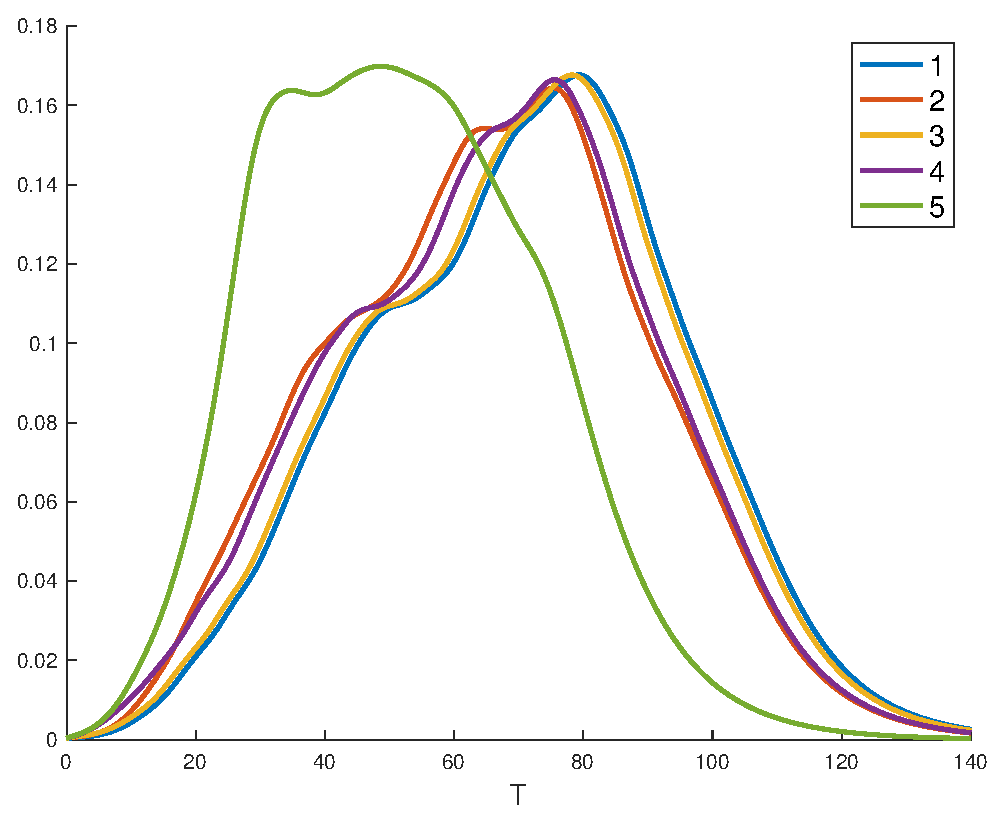
\includegraphics[scale=0.45]{Figure/minnesota_prevalenza}
\caption[Grafico della prevalenza al variare del grado del nodo inizialmente infetto.]{Grafico della prevalenza al variare del grado del nodo inizialmente infetto.\\ Per ottenere i grafici abbiamo risolto numericamente, usando MATLAB, cinque problema di Cauchy ottenuti dal modello chiuso alle coppie.\\
Per le condizioni iniziali abbiamo preso ogni volta un nodo certamente infetto (con grado diverso e tutti gli altri nodi certamente sani).\\
Per la sperimentazione abbiamo utilizzato come parametri $\tau=0.3$ e $\gamma=0.1$}
\label{fig::minnesota_prevalenza}
\end{figure}



\chapter*{Conclusioni}
 \addcontentsline{toc}{chapter}{Conclusioni}
Concludiamo questa tesi sottolineando alcune limitazioni presenti nel modello SIR presentato.\\
La suddivisione delle popolazione in tre compartimenti non garantisce una grande generalit\`a. Ad esempio, utilizzando questo modello non possiamo considerare il tempo di incubazione ovvero il periodo di tempo tra l'infezione e il momento in cui un individuo diventa infettivo (trasmette la malattia). Per ovviare a questo problema si pu\`o  considerare una generalizzazione del modello SIR: il modello  SEIR dove  abbiamo aggiunto la classe E degli ``esposti" ovvero degli infetti che  non sono infettivi. Le equazione~\eqref{SIR} diventano dunque 
\begin{equation*}
\begin{aligned}
S' &= -\beta S I \\
E' &= \beta S I  - \eta  E \\
I' &= aE - \alpha I \\
R' &=\alpha I 
\end{aligned}
\end{equation*}
dove il periodo medio d'incubazione \`e $\eta^{-1}$.\\
In analogia a quanto fatto nel secondo capitolo, potremmo estendere il modello SEIR ad una rete.\\
\\
Un altro aspetto limitante del modello SIR \`e che esso non tiene conto delle politiche di contenimento: il numero medio di contatti efficaci (contatti che provocano l'infezione) non pu\`o e non deve essere costante. Pensiamo, ad esempio, alle varie misure adottate per contrastare la diffusione di COVID-19 finalizzate a ridurre questo numero: lockdown, distanziamento sociale, uso delle mascherine, ...\\ \\
Abbiamo visto il legame tra parametri e stiffness per la rete del Minnesota, sarebbe interessante investigare come varia questo legame per vari tipi di network sia reali che randomici: small-world, scale-free ... .\\
\bibliography{references}
\addcontentsline{toc}{chapter}{Bibliografia}
\bibliographystyle{plain}

\cleardoublepage
\listoffigures
\addcontentsline{toc}{chapter}{Elenco delle figure}
\listoftables
\addcontentsline{toc}{chapter}{Elenco delle tabelle}
\tableofcontents

\end{document}